% !TeX program = xelatex
% ==================================================================
%  徐森林、薛春华《数学分析》（第二册）
%  按《中文数学书籍 LaTeX 重排规范》v2.1 重排
%  编译：xelatex -> biber -> xelatex x3（见 tools/build.py）
% ==================================================================
\documentclass[
  BookTitleCN     = {数学分析},
  BookTitleCNSub  = {第二册},
  AuthorCN        = {徐森林\quad 薛春华},
  Publisher       = {清华大学出版社},
  Year            = {2006},
  ISBN            = {978-7-302-13141-0},
  Biblatex        = true,
  BibStyle        = numeric,
  BibSorting      = none,
  BibFile         = refs,
  StartPage       = 1
]{zhmbook}

\begin{document}

\frontmatter
\maketitle

% ==================================================================
%  chapters/preface.tex —— 原书前言 (p. I ~ II)
%  严格遵循《中文数学书籍 LaTeX 重排规范》：英文标点、忠实原文
% ==================================================================

\chapter*{前言}
\addcontentsline{toc}{chapter}{前言}
\markboth{前言}{前言}

数学分析是数学专业最重要的基础课, 它对后继课程 (实变函数, 泛函分析, 拓扑, 微分几何) 与近代数学的学习与研究具有非常深远的影响和至关重要的作用. 一本优秀的数学分析教材必须包含传统微积分内容的精髓和分析能力与方法的传授, 也必须包含近代的内容, 其检验标准是若干年后能否涌现出一批高水准的应用数学人才和数学研究人才, 特别是一些数学顶尖人物. 作者从事数学分析教学几十年, 继承导师, 著名数学家吴文俊教授的一整套教学 (特别是教授数学分析的) 方法 (科大称之为``吴龙''), 并将其发扬光大, 因材施教, 在中国科技大学培养了一批国内外有名的数学家与数学工作者. 目前, 作者徐森林被特聘到华中师范大学数学与统计学学院, 并在数学试点班用此教材讲授数学分析, 效果显著.

本书的主要特色可归纳为以下几点.

\section*{1. 传统精髓内容的完善化}

书中包含了实数的各种引入, 七个实数连续性等价命题的论述; 给出了单变量与多变量的 Riemann 可积的各等价命题的证明; 讨论了微分中值定理, Taylor 公式余项的各种表达; 介绍了积分第一, 第二中值定理的描述, 隐函数存在性定理与反函数定理的两种不同的证法等内容.

\section*{2. 与后继课程的紧密结合, 使内容近代化}

本书在介绍经典微积分理论的同时, 将近代数学中许多重要概念, 理论恰到好处地引进分析教材中. 例如, 在积分理论中, 给出了 Lebesgue 定理: 函数 $f$ Riemann 可积的充要条件是 $f$ 几乎处处连续且有界; 详细讨论了 $\mathbb{R}^n$ 中的拓扑及相应的开集, 闭集, 聚点等概念, 描述了 $\mathbb{R}^n$ 中集合的紧致性, 连通性, 可数性, Hausdorff 性等拓扑不变性, 使读者站到拓扑的高度来理解零值定理, 介值定理, 最值定理与一致连续性定理. 引进外微分形式及外微分运算, 将经典 Newton-Leibniz 公式, 平面 Green 公式, 空间 Stokes 公式与 Gauss 公式统一为 Stokes 公式, 并对闭形式, 恰当形式与场论的对偶关系给出了全新的表述. 这不仅使教材内容本身近代化, 而且为学生在高年级学习拓扑, 实变函数, 泛函分析, 微分几何等课程提供了一个实际模型并打下良好的基础, 为经典数学与近代数学架设了一座桥梁.

\section*{3. 因材施教, 着重培养学生的研究与创新能力}

同一定理 (如零值定理, 一致连续性定理, Lagrange 中值定理, Cauchy 中值定理, 隐函数存在性定理与反函数定理等) 经常采用多种证法; 同一例题应用不同定理或不同方法解答, 这是本书又一特色. 它使学生广开思路, 积极锻炼思维能力, 使思维越来越敏捷与成熟. 书中举出大量例题是为了让读者得到一定的基本训练, 同时从定理的证明和典型实例的分析中掌握数学分析的技巧与方法. 习题共分三个层次: 练习题, 思考题与复习题. 练习题是基本题, 是为读者熟练掌握内容与方法设置的. 为提高学生对数学的浓厚兴趣及解题的能力, 设置了思考题. 为了让读者减少做题的障碍, 增强对数学的自信心, 其中有些题给出了提示. 实际上, 该节的标题就是最好的提示. 在每一章设置了大量复习题, 这些题不给提示, 因此大部分学生对它们会感到无从下手, 这些题是为少数想当数学家的学生特别设置的, 希望他们能深入思考, 自由发挥, 将它们一个一个地解答出来, 为将来的研究培养自己的创新能力. 如有困难, 我们还可撰写一本精练的学习指导书.

本书共分三册. 第一册内容包括数列极限, 函数极限与连续, 一元函数的导数与微分中值定理, Taylor 公式, 不定积分以及 Riemann 积分; 第二册内容包括 $\mathbb{R}^n$ 中的拓扑, $n$ 元函数的极限与连续, $n$ 元函数的微分学, 隐函数定理与反函数定理, $n$ 重积分, 第一型曲线, 曲面积分, 第二型曲线, 曲面积分, Stokes 定理, 外微分形式与场论; 第三册内容包括数项级数和各种收敛判别法, 函数项级数的一致收敛性及其性质, 含参变量反常积分的一致收敛性及其性质, Euler 积分 ($\Gamma$ 函数与 $B$ 函数), 幂级数与 Taylor 级数, Fourier 分析.

在写作本书的时候, 得到了华中师范大学数学与统计学学院领导和教师们的热情鼓励与大力支持, 作者们谨在此对他们表示诚挚的感谢. 博士生邓勤涛, 胡自胜, 薛琼, 硕士生金亚东, 鲍焱红等对本书的写作提出了许多宝贵意见, 使本书增色不少.

特别还要感谢的是清华大学出版社的曾刚, 刘颖, 王海燕, 他们为我们提供了本书出版的机会, 了却了我多年的心愿.

\vspace{1.5\baselineskip}
\begin{flushright}
  徐森林\\
  2005\,年\,6\,月于武汉
\end{flushright}


\tableofcontents

\mainmatter

% 本书为《数学分析》第二册，正文起自第 7 章，
% 将章计数器设为 6，使首个 \chapter 自增后为「第 7 章」。
% 正文起始页码设为 1，与原书对齐。
\setcounter{chapter}{6}
\setcounter{page}{1}

% 第 7 章（已完成）
% ==================================================================
%  徐森林、薛春华《数学分析》（第二册）
%  第 7 章  (R^n, \rho_0^n) 的拓扑、n 元函数的连续与极限
% ==================================================================

\chapter{\texorpdfstring{$(R^n, \rho_0^n)$}{(R^n, ρ)} 的拓扑、n 元函数的连续与极限}\label{ch:7}

从极限理论和实数理论导出了闭区间 $[a, b]$ 上连续函数的零值定理, 介值定理, 最值定理及一致连续性定理, 要将这些定理推广到 $n$ 维 Euclid 空间 $R^n$ 中, 必须介绍 $R^n$ 及其子集的拓扑的确切定义, 随之而来的还有开集, 闭集, 聚点, 收敛, 紧致性, 连通性等重要概念. 本章证明了 $R^n$ 中子集 $A$ 的紧致, 可数紧致, 列紧, 序列紧致都等价于 $A$ 为 $R^n$ 中的有界闭集; 连通集上的连续函数有零值定理与介值定理; 紧致集上的连续函数有最值定理及一致连续性定理. 上述内容是站在度量空间, 拓扑空间高度来叙述的. 考虑到 Euclid 空间 $R^n$ 这一特定的度量空间, 特定的拓扑空间, 我们还需讨论 $n$ 元函数的极限及相关的定理.

% ==================================================================
%  §7.1  (R^n, \rho_0^n) 的拓扑
%  源：徐森林、薛春华《数学分析》第二册，印刷页 1-15 (PDF p. 7-21)
%  底本：PaddleOCR-VL-1.6 JSON/MD 识别结果，人工逐字核校与公式精修
%  规范：全西文标点，忠实原文定理、定义、引理、例题、练习题编号与推导
% ==================================================================

\section{\texorpdfstring{$(R^n, \rho_0^n)$}{(R^n, ρ_0^n)} 的拓扑}

为了培养读者抽象思维能力, 我们采用从抽象到具体的方法, 在非空集合上引进拓扑的概念, 然后给出度量空间 $(X, \rho)$ 诱导的拓扑空间 $(X, \mathcal{T}_{\rho})$, 作为特殊度量空间的 Euclid 空间 $(R^n, \rho_0^n)$, 它相应的拓扑空间为 $(R^n, \mathcal{T}_{\rho_0^n})$, 而 $\mathcal{T}_{\rho_0^n}$ 就是 $R^n$ 中的通常拓扑.

\begin{definition}\label{def:7.1.1}
如果非空集合 $X$ 的子集族
\[
  \mathcal{T}=\{U \mid U\text{ 具有性质 } *\}
\]
满足:
\begin{enumerate}
  \item $X, \varnothing \in \mathcal{T}$;
  \item 若 $U_1, U_2 \in \mathcal{T}$, 则 $U_1 \cap U_2 \in \mathcal{T}$;
  \item $\bigcup_{U \in \mathcal{T}_0 \subset \mathcal{T}} U \in \mathcal{T}$ (或表达为: 若 $U_\alpha \in \mathcal{T}, \alpha \in \Gamma$ (指标集), 必有 $\bigcup_{\alpha \in \Gamma} U_\alpha \in \mathcal{T}$).
\end{enumerate}
则称 $\mathcal{T}$ 为 $X$ 上的一个\textbf{拓扑}, $(X, \mathcal{T})$ 称为 $X$ 上的一个\textbf{拓扑空间}.

$U \in \mathcal{T}$ 称为 $(X, \mathcal{T})$ 中的\textbf{开集}. 如果 $F$ 的余 (补) 集 $F^c = X \setminus F \in \mathcal{T}$, 则称 $F$ 为 $(X, \mathcal{T})$ 中的\textbf{闭集}. 由数学归纳法与 (2) 知, 有限个开集的交为开集; 由 (3) 知, 任意多个开集的并为开集.
\end{definition}

\begin{definition}\label{def:7.1.2}
设 $(X, \mathcal{T})$ 为拓扑空间, $A \subset X$, $x \in X$ (不必属于 $A$). 如果对 $x$ 的任何开邻域 (含 $x$ 的开集) $U$, 必有
\[
  U \cap (A \setminus \{x\}) = (U \setminus \{x\}) \cap A \neq \varnothing,
\]
则称 $x$ 为 $A$ 的\textbf{聚点}. 记 $A$ 的聚点的全体为 $A'$ 或 $A^d$, 称为 $A$ 的\textbf{导集}. 而 $\overline{A} = A \cup A'$ 称为 $A$ 的\textbf{闭包}, 有时记 $\overline{A}$ 为 $A^-$. 如果 $\overline{A} = X$, 则称 $A$ 为 $(X, \mathcal{T})$ 的\textbf{稠密集}.

如果 $a \in A$, 且 $a \notin A'$, 则称 $a$ 为 $A$ 的\textbf{孤立点}. 显然,
\[
  a\text{ 为 } A\text{ 的孤立点} \iff a \in A\text{ 且 }\exists U_0 \in \mathcal{T},\text{ s.t. } U_0 \cap A = \{a\}.
\]
\end{definition}

\begin{theorem}\label{thm:7.1.1}
$x \in \overline{A} \iff$ 对 $x$ 的任何开邻域 $U$, 有 $U \cap A \neq \varnothing$.

等价地, 有
\[
  x \notin \overline{A} \iff \text{存在 } x \text{ 的开邻域 } U_0,\text{ 使得 } U_0 \cap A = \varnothing.
\]
\end{theorem}

\begin{proof}
$x \in \overline{A} = A \cup A' \iff x \in A$ 或 $x \notin A, x \in A' \iff$ 对 $x$ 的任何开邻域 $U$, 有 $U \cap A \neq \varnothing$. \qedhere
\end{proof}

\begin{lemma}[De Morgan 公式]\label{lem:7.1.1}
\[
  X \setminus \bigcup_{\alpha \in \Gamma} A_\alpha = \bigcap_{\alpha \in \Gamma} (X \setminus A_\alpha), \qquad
  X \setminus \bigcap_{\alpha \in \Gamma} A_\alpha = \bigcup_{\alpha \in \Gamma} (X \setminus A_\alpha).
\]
如果 $A_\alpha \subset X\ (\forall \alpha \in \Gamma)$, 则称 $X$ 为全空间. 上述两式变为
\[
  \left(\bigcup_{\alpha \in \Gamma} A_\alpha\right)^c = \bigcap_{\alpha \in \Gamma} A_\alpha^c, \qquad
  \left(\bigcap_{\alpha \in \Gamma} A_\alpha\right)^c = \bigcup_{\alpha \in \Gamma} A_\alpha^c.
\]
\end{lemma}

\begin{proof}
由
\begin{align*}
  x \in X \setminus \bigcup_{\alpha \in \Gamma} A_\alpha
  &\iff x \in X,\ x \notin \bigcup_{\alpha \in \Gamma} A_\alpha \\
  &\iff x \in X,\ \forall \alpha \in \Gamma,\ x \notin A_\alpha \\
  &\iff \forall \alpha \in \Gamma,\ x \in (X \setminus A_\alpha) \\
  &\iff x \in \bigcap_{\alpha \in \Gamma} (X \setminus A_\alpha)
\end{align*}
知第一式成立. 类似可证第二式. \qedhere
\end{proof}

\begin{theorem}[闭集性质]\label{thm:7.1.2}
设 $\mathcal{F}$ 为拓扑空间 $(X, \mathcal{T})$ 中所有闭集的族, 则:
\begin{enumerate}
  \item $X, \varnothing \in \mathcal{F}$;
  \item 若 $F_1, F_2 \in \mathcal{F}$, 则 $F_1 \cup F_2 \in \mathcal{F}$;
  \item $\bigcap_{F \in \mathcal{F}_0 \subset \mathcal{F}} F \in \mathcal{F}$ (或表达为: 若 $F_\alpha \in \mathcal{F}, \alpha \in \Gamma$, 必有 $\bigcap_{\alpha \in \Gamma} F_\alpha \in \mathcal{F}$).
\end{enumerate}
由数学归纳法与 (2) 知, 有限个闭集的并为闭集; 由 (3) 知, 任意个闭集的交为闭集.
\end{theorem}

\begin{proof}
(1) 因为 $X^c = \varnothing \in \mathcal{T}$, $\varnothing^c = X \in \mathcal{T}$, 所以 $X, \varnothing \in \mathcal{F}$.

(2) 因为 $F_1, F_2 \in \mathcal{F}$, 所以 $F_1^c, F_2^c \in \mathcal{T}$,
\[
  (F_1 \cup F_2)^c \reason{De Morgan 公式} F_1^c \cap F_2^c \in \mathcal{T},
\]
从而 $F_1 \cup F_2 \in \mathcal{F}$.

(3) 因为 $F_\alpha \in \mathcal{F}$, 所以 $F_\alpha^c \in \mathcal{T}, \alpha \in \Gamma$. 于是,
\[
  \left(\bigcap_{\alpha \in \Gamma} F_\alpha\right)^c \reason{De Morgan 公式} \bigcup_{\alpha \in \Gamma} F_\alpha^c \in \mathcal{T},
\]
从而 $\bigcap_{\alpha \in \Gamma} F_\alpha \in \mathcal{F}$. \qedhere
\end{proof}

\begin{theorem}[导集性质]\label{thm:7.1.3}
设 $(X, \mathcal{T})$ 为拓扑空间, $A, B \subset X$, 则:
\begin{enumerate}
  \item $\varnothing' = \varnothing$;
  \item 若 $A \subset B$, 则 $A' \subset B'$;
  \item $(A \cup B)' = A' \cup B'$;
  \item $\forall a \in A'$, $(A \setminus \{a\})' = A'$.
\end{enumerate}
\end{theorem}

\begin{proof}
(1) 显然 $\varnothing' = \varnothing$.

(2) 设 $x \in A'$, 则对 $x$ 的任何开邻域 $U$, 有
\[
  \varnothing \neq U \cap (A \setminus \{x\}) \subset U \cap (B \setminus \{x\}),
\]
即 $x \in B'$, 故 $A' \subset B'$.

(3) 由 $A \subset A \cup B, B \subset A \cup B$ 以及 (2) 得到 $A' \subset (A \cup B)', B' \subset (A \cup B)'$, 从而 $A' \cup B' \subset (A \cup B)'$.

反之, 设 $x \notin A' \cup B'$, 则 $x \notin A'$ 且 $x \notin B'$. 于是, 存在 $x$ 的开邻域 $U_1, U_2 \in \mathcal{T}$, s.t.
\[
  U_1 \cap (A \setminus \{x\}) = \varnothing, \qquad U_2 \cap (B \setminus \{x\}) = \varnothing.
\]
令 $U = U_1 \cap U_2 \in \mathcal{T}$, 显然 $U$ 为 $x$ 的开邻域, 且
\[
  U \cap ((A \cup B) \setminus \{x\}) = (U \cap (A \setminus \{x\})) \cup (U \cap (B \setminus \{x\})) = \varnothing,
\]
所以 $x \notin (A \cup B)'$. 这就证明了 $(A \cup B)' \subset A' \cup B'$. 综上所述, $(A \cup B)' = A' \cup B'$.

(4) 类似可证 $\forall a \in A', (A \setminus \{a\})' = A'$. \qedhere
\end{proof}

\begin{theorem}[闭包性质]\label{thm:7.1.4}
设 $(X, \mathcal{T})$ 为拓扑空间, $A, B \subset X$, 则:
\begin{enumerate}
  \item $\overline{\varnothing} = \varnothing$;
  \item 若 $A \subset B$, 则 $\overline{A} \subset \overline{B}$;
  \item $\overline{A \cup B} = \overline{A} \cup \overline{B}$;
  \item $\overline{\overline{A}} = \overline{A}$;
  \item $A$ 为闭集 $\iff A = \overline{A} \iff A' \subset A$.
\end{enumerate}
\end{theorem}

\begin{proof}
(1) $\overline{\varnothing} = \varnothing \cup \varnothing' = \varnothing \cup \varnothing = \varnothing$.

(2) 由 $A \subset B$ 与 \cref{thm:7.1.3}(2) 得到 $A' \subset B'$, 从而
\[
  \overline{A} = A \cup A' \subset B \cup B' = \overline{B}.
\]

(3) $\overline{A \cup B} = (A \cup B) \cup (A \cup B)' \reason{\cref{thm:7.1.3}(3)} (A \cup B) \cup (A' \cup B') = (A \cup A') \cup (B \cup B') = \overline{A} \cup \overline{B}$.

(4) 显然, $\overline{A} \subset \overline{A} \cup (\overline{A})' = \overline{\overline{A}}$. 进而, 有
\begin{align*}
  x \in \overline{\overline{A}}
  &\xleftrightarrow{\text{\cref{thm:7.1.1}}} \text{对 } x \text{ 的任何开邻域 } U, U \cap \overline{A} \neq \varnothing \\
  &\xleftrightarrow{\quad} \text{对 } x \text{ 的任何开邻域 } U, U \cap A \neq \varnothing \\
  &\xleftrightarrow{\text{\cref{thm:7.1.1}}} x \in \overline{A}.
\end{align*}
所以, $\overline{\overline{A}} = \overline{A}$.

(5) 由定义, $A = \overline{A} = A \cup A' \iff A' \subset A$. 现证 $A$ 为闭集 $\iff A = \overline{A}$.

($\Rightarrow$) 设 $A$ 为闭集, 则 $A^c = X \setminus A \in \mathcal{T}$ 为开集. $\forall x \notin A$, 则 $x \in A^c$, 取 $U_0 = A^c \in \mathcal{T}$, 有 $U_0 \cap A = \varnothing$. 由 \cref{thm:7.1.1} 知 $x \notin \overline{A}$. 这表明 $\overline{A} \subset A$, 从而 $\overline{A} = A$.

($\Leftarrow$) 设 $A = \overline{A}$. $\forall x \in A^c = X \setminus A = X \setminus \overline{A}$, 由 \cref{thm:7.1.1} 知存在 $x$ 的开邻域 $U_x$, 使得 $U_x \cap A = \varnothing$, 即 $U_x \subset A^c$. 于是 $A^c = \bigcup_{x \in A^c} U_x \in \mathcal{T}$, 即 $A^c$ 为开集, 从而 $A$ 为闭集. \qedhere
\end{proof}

\begin{definition}\label{def:7.1.3}
设 $\{x_n\}$ 为 $(X, \mathcal{T})$ 中的点列. 如果 $\exists x \in X$, 对 $x$ 的任何开邻域 $U$, $\exists N \in \mathbb{Z}_+$, 当 $n > N$ 时, 有 $x_n \in U$, 则称 $\{x_n\}$ \textbf{收敛于} $x$, 记作 $\lim_{n \to \infty} x_n = x$ 或 $x_n \to x\ (n \to \infty)$, 而 $x$ 称为点列 $\{x_n\}$ 的\textbf{极限}.
\end{definition}

\begin{theorem}\label{thm:7.1.5}
设 $(X, \mathcal{T})$ 为拓扑空间, 点列 $\{x_n\} \subset X$, 则
\[
  \lim_{n \to \infty} x_n = x \implies x \in \overline{\{x_n\}}.
\]
\end{theorem}

\begin{proof}
根据定义, 对 $x$ 的任何开邻域 $U$, $\exists N \in \mathbb{Z}_+$, 当 $n > N$ 时, $x_n \in U$. 于是 $U \cap \{x_n\} \neq \varnothing$. 根据 \cref{thm:7.1.1}, $x \in \overline{\{x_n\}}$. \qedhere
\end{proof}

\begin{definition}\label{def:7.1.4}
设 $X$ 为非空集合, 映射 $\rho: X \times X \to \mathbb{R}$ 满足:
\begin{enumerate}
  \item $\rho(x, y) \geqslant 0$, 且 $\rho(x, y) = 0 \iff x = y$ (正定性);
  \item $\rho(x, y) = \rho(y, x)$ (对称性);
  \item $\rho(x, z) \leqslant \rho(x, y) + \rho(y, z)$ (三角不等式).
\end{enumerate}
则称 $\rho$ 为 $X$ 上的一个\textbf{度量} (或\textbf{距离}), $(X, \rho)$ 称为 $X$ 上的一个\textbf{度量 (距离) 空间}, $\rho(x, y)$ 称为点 $x$ 与 $y$ 的距离.

现在验证: 度量空间 $(X, \rho)$ 上的子集族
\[
  \mathcal{T}_\rho = \{U \mid \forall x \in U, \exists \delta > 0,\text{ s.t. 开球 } B(x; \delta) \subset U\}
\]
为 $X$ 上的一个拓扑, 称为由 $\rho$ \textbf{诱导的拓扑}, 其中 $B(x; \delta) = \{y \mid y \in X, \rho(y, x) < \delta\}$ 是以 $x$ 为中心, $\delta$ 为半径的\textbf{开球}.
\end{definition}

\begin{proof}[验证 $\mathcal{T}_\rho$ 为拓扑]
(1) 由于 $\forall x \in X$, 显然有 $B(x; 1) \subset X$, 故 $X \in \mathcal{T}_\rho$. 因为 $\varnothing$ 不含任何元素, 满足开集性质, 故 $\varnothing \in \mathcal{T}_\rho$.

(2) 设 $U_1, U_2 \in \mathcal{T}_\rho$. 若 $U_1 \cap U_2 = \varnothing$, 显然属于 $\mathcal{T}_\rho$. 若 $U_1 \cap U_2 \neq \varnothing$, 则 $\forall x \in U_1 \cap U_2$, 有 $x \in U_i$, 存在 $\delta_i > 0$ 使得 $B(x; \delta_i) \subset U_i\ (i = 1, 2)$. 取 $\delta = \min\{\delta_1, \delta_2\} > 0$, 则 $B(x; \delta) \subset U_1 \cap U_2$, 故 $U_1 \cap U_2 \in \mathcal{T}_\rho$.

(3) 设 $U_\alpha \in \mathcal{T}_\rho\ (\alpha \in \Gamma)$. 若 $x \in \bigcup_{\alpha \in \Gamma} U_\alpha$, 则存在 $\alpha_0 \in \Gamma$ 使得 $x \in U_{\alpha_0}$. 存在 $\delta_0 > 0$ 使得 $B(x; \delta_0) \subset U_{\alpha_0} \subset \bigcup_{\alpha \in \Gamma} U_\alpha$, 故 $\bigcup_{\alpha \in \Gamma} U_\alpha \in \mathcal{T}_\rho$. \qedhere
\end{proof}

\begin{theorem}\label{thm:7.1.6}
设 $(X, \rho)$ 为度量空间, $A \subset X, x \in X$, 则下列命题等价:
\begin{enumerate}
  \item $x \in A'$;
  \item $x$ 的任何开邻域 $U$ 中含 $A$ 的无限多个点;
  \item $\exists \{x_k\} \subset A$, 使得 $x_k$ 互异, $x_k \neq x$, 且 $\lim_{k \to \infty} x_k = x$.
\end{enumerate}
\end{theorem}

\begin{proof}
(1) $\Rightarrow$ (3): 设 $x \in A'$, 对 $x$ 的任何开邻域 $U$, $\exists n_1 \in \mathbb{Z}_+$, s.t. $B(x; 1/n_1) \subset U$, 则有 $x_1 \in B(x; 1/n_1) \cap (A \setminus \{x\})$. 取 $n_2 > n_1$, s.t. $1/n_2 < \rho(x_1, x)$, 则对 $x$ 的开邻域 $B(x; 1/n_2)$, 有 $x_2 \in B(x; 1/n_2) \cap (A \setminus \{x\})$, 显然 $x_2 \neq x_1$. 依此类推, 得到 $\{x_k\}$, s.t. $x_k \in B(x; 1/n_k) \cap (A \setminus \{x\})$, 且 $x_k$ 互异且 $x_k \neq x$. 由 $0 \leqslant \rho(x_k, x) < 1/n_k \to 0\ (k \to \infty)$ 得到 $\lim_{k \to \infty} x_k = x$.

(2) $\Leftrightarrow$ (3): 对 $x$ 的任何开邻域 $U$, 因为 $\lim_{k \to \infty} x_k = x$, 故存在 $K \in \mathbb{Z}_+$, 当 $k > K$ 时, 有 $x_k \in U$. 由于 $x_k$ 互异, 知 $U$ 中含 $A$ 的无限个点.

(2) $\Rightarrow$ (1): 显然. \qedhere
\end{proof}

\begin{example}\label{ex:7.1.1}
设 $X$ 为非空集合, $\mathcal{T}_{\text{平庸}} = \{\varnothing, X\}$. 显然 $\mathcal{T}_{\text{平庸}}$ 为 $X$ 上的一个拓扑, 其开集最少, 称 $(X, \mathcal{T}_{\text{平庸}})$ 为 $X$ 上的\textbf{平庸拓扑空间}.

当 $X = \{a, b\}\ (a \neq b)$ 时, $\mathcal{T}_{\text{平庸}} = \{\varnothing, \{a, b\}\}$. 取 $A = \{a\}$, 则 $A' = \{b\}$. 显然, $b$ 的任何开邻域 $U$ 必为 $X = \{a, b\}$, 它只含 $A = \{a\}$ 的一个点 $a$, 而不是无限个点. 这表明 \cref{thm:7.1.6} 中的性质 (2), (3) 是度量空间中特有的性质.
\end{example}

\begin{definition}\label{def:7.1.5}
设 $(X, \mathcal{T})$ 为拓扑空间, $x \in X$. $x$ 的一个开邻域族 $\mathcal{T}_x^*$, 若对 $x$ 的任何开邻域 $U$, 均有 $U_0 \in \mathcal{T}_x^*$, s.t. $x \in U_0 \subset U$, 则称 $\mathcal{T}_x^*$ 为 $x$ 的一个\textbf{局部基}. 若 $\mathcal{T}_x^*$ 为至多可数集, 则称 $\mathcal{T}_x^*$ 为 $x$ 的一个\textbf{可数局部基}.

如果 $\forall x \in X$ 均有可数局部基, 则称 $(X, \mathcal{T})$ 为 $A_1$ \textbf{空间}或具有\textbf{第一可数性公理}的拓扑空间.

如果有 $\mathcal{T}^* \subset \mathcal{T}$, 对 $\mathcal{T}$ 中任一元素 $U$, 有 $U = \bigcup_{V \in \mathcal{T}_0^* \subset \mathcal{T}^*} V$ (即 $\forall x \in U, \exists V \in \mathcal{T}^*$, s.t. $x \in V \subset U$), 则称 $\mathcal{T}^*$ 为 $(X, \mathcal{T})$ 的一个\textbf{拓扑基}. 进而, 当 $\mathcal{T}^*$ 为至多可数集时, 称 $\mathcal{T}^*$ 为可数拓扑基, 并称 $(X, \mathcal{T})$ 为 $A_2$ \textbf{空间}或具有\textbf{第二可数性公理}的拓扑空间.
\end{definition}

\begin{example}\label{ex:7.1.2}
设 $(X, \rho)$ 为度量空间, 则 $\forall x \in X$,
\[
  \mathcal{T}_x^* = \left\{B\left(x; \frac{1}{n}\right) \;\middle|\; n \in \mathbb{Z}_+\right\}
\]
为 $x$ 处的一个可数局部基. 事实上, $\forall U \in \mathcal{T}_\rho$ (含 $x$ 的开集), $\exists \delta > 0$, s.t. $B(x; \delta) \subset U$, 取 $N \in \mathbb{Z}_+$ 满足 $1/N < \delta$, 则 $x \in B(x; 1/N) \subset B(x; \delta) \subset U$. 故任何度量空间都是 $A_1$ 空间.
\end{example}

\begin{theorem}\label{thm:7.1.7}
设 $(X, \mathcal{T})$ 为 $A_1$ 空间, $A \subset X, x \in X$, 则:
\begin{enumerate}
  \item $x \in A' \iff \exists \{x_n\} \subset A \setminus \{x\}$, 使得 $\lim_{n \to \infty} x_n = x$;
  \item $x \in \overline{A} \iff \exists \{x_n\} \subset A$, 使得 $\lim_{n \to \infty} x_n = x$.
\end{enumerate}
\end{theorem}

\begin{proof}
(1) ($\Leftarrow$) 设 $\{x_n\} \subset A \setminus \{x\}$ 且 $\lim_{n \to \infty} x_n = x$, 则对 $x$ 的任何开邻域 $U$, 存在 $N$, 当 $n > N$ 时 $x_n \in U \cap (A \setminus \{x\}) \neq \varnothing$, 故 $x \in A'$.

($\Rightarrow$) 设 $x \in A'$. 设 $\{U_n \mid n \in \mathbb{Z}_+\}$ 为 $x$ 处的可数局部基, 令 $V_n = \bigcap_{i=1}^n U_i$, 则 $V_1 \supset V_2 \supset \cdots$, 称为规范可数局部基. 因 $x \in A'$, 故对每个 $n$, $V_n \cap (A \setminus \{x\}) \neq \varnothing$. 取 $x_n \in V_n \cap (A \setminus \{x\})$, 易见 $\lim_{n \to \infty} x_n = x$.

(2) 类似可由 (1) 推得. \qedhere
\end{proof}

\begin{theorem}\label{thm:7.1.8}
设 $(X, \mathcal{T})$ 为 $A_1$ 空间, 则
\[
  A \text{ 为闭集} \iff \forall \{x_n\} \subset A,\ \lim_{n \to \infty} x_n = x \implies x \in A.
\]
\end{theorem}

\begin{proof}
($\Rightarrow$) 由 \cref{thm:7.1.5}, $\lim_{n \to \infty} x_n = x \implies x \in \overline{A}$. 若 $A$ 为闭集, 则 $\overline{A} = A$, 故 $x \in A$.

($\Leftarrow$) (反证) 假设 $A$ 不为闭集, 则 $\exists x \in A', x \notin A$. 由 \cref{thm:7.1.7}, 存在 $\{x_n\} \subset A$ 使得 $\lim_{n \to \infty} x_n = x$. 但 $x \notin A$, 矛盾. \qedhere
\end{proof}

\begin{definition}\label{def:7.1.6}
设 $(X, \mathcal{T})$ 为拓扑空间. 如果 $\forall p, q \in X, p \neq q$, 均存在 $p$ 的开邻域 $U$ 与 $q$ 的开邻域 $V$, 使得 $U \cap V = \varnothing$, 则称 $(X, \mathcal{T})$ 为 $T_2$ \textbf{空间}或 \textbf{Hausdorff 空间}.
\end{definition}

\begin{theorem}\label{thm:7.1.9}
设 $(X, \mathcal{T})$ 为 $T_2$ 空间, 点列 $\{x_n\} \subset X$ 收敛, 则极限是惟一的.
\end{theorem}

\begin{proof}
(反证) 假设极限不唯一, 存在 $x \neq y$, 使得 $\lim_{n \to \infty} x_n = x$ 且 $\lim_{n \to \infty} x_n = y$. 因为 $(X, \mathcal{T})$ 为 $T_2$ 空间, 存在开邻域 $U \ni x, V \ni y$ 满足 $U \cap V = \varnothing$. 但由极限定义, 当 $n$ 充分大时 $x_n \in U$ 且 $x_n \in V$, 即 $x_n \in U \cap V = \varnothing$, 矛盾. \qedhere
\end{proof}

\begin{example}\label{ex:7.1.3}
平庸拓扑空间 $(X, \mathcal{T}_{\text{平庸}})$ 当点数大于 1 时显然不是 $T_2$ 空间.
\end{example}

\begin{lemma}\label{lem:7.1.2}
任何度量空间 $(X, \rho)$ 均为 $T_2$ 空间.
\end{lemma}

\begin{proof}
$\forall p \neq q$, 取 $\delta = \frac{1}{2}\rho(p, q) > 0$. 令 $U = B(p; \delta), V = B(q; \delta)$, 则 $U, V$ 分别为 $p, q$ 的开邻域, 且由三角不等式易见 $U \cap V = \varnothing$. \qedhere
\end{proof}

\begin{example}\label{ex:7.1.4}
设 $X$ 为非空集合, 定义离散度量
\[
  \rho(x, y) = \begin{cases}
    1, & x \neq y, \\
    0, & x = y.
  \end{cases}
\]
则诱导拓扑为离散拓扑 $\mathcal{T}_{\text{离散}} = \mathcal{P}(X)$ (每一个子集都是开集, 也都是闭集).
\end{example}

\begin{example}\label{ex:7.1.5}
设 $(X, \rho)$ 为度量空间, $Y \subset X$ 为非空集合. 限制 $\rho_Y = \rho|_{Y \times Y}$ 使 $(Y, \rho_Y)$ 成为子度量空间, 其开球满足 $B_Y(x; \delta) = B(x; \delta) \cap Y$.
\end{example}

\begin{example}\label{ex:7.1.6}
设 $(X, \mathcal{T})$ 为拓扑空间, $Y \subset X$ 为非空子集. 记 $\mathcal{T}_Y = \{U \cap Y \mid U \in \mathcal{T}\}$, 则 $\mathcal{T}_Y$ 为 $Y$ 上的拓扑, 称为\textbf{子空间拓扑}或\textbf{诱导拓扑}.
\end{example}

\begin{corollary}\label{cor:7.1.1}
设 $(X, \rho)$ 为度量空间, 则:
\begin{enumerate}
  \item $A$ 为闭集 $\iff \forall \{x_n\} \subset A, \lim_{n \to \infty} x_n = x \implies x \in A$;
  \item 如果点列 $\{x_n\} \subset X$ 收敛, 则极限是惟一的.
\end{enumerate}
\end{corollary}

\begin{lemma}[Cauchy-Schwarz 不等式]\label{lem:7.1.3}
对任意 $x = (x_1, \dots, x_n), y = (y_1, \dots, y_n) \in \mathbb{R}^n$, 有
\[
  |\langle x, y \rangle| \leqslant \|x\| \|y\|, \quad\text{即}\quad
  \left(\sum_{i=1}^n x_i y_i\right)^2 \leqslant \left(\sum_{i=1}^n x_i^2\right) \left(\sum_{i=1}^n y_i^2\right).
\]
\end{lemma}

\begin{lemma}[Minkowski 不等式]\label{lem:7.1.4}
对任意 $x, y \in \mathbb{R}^n$, 有
\[
  \|x + y\| \leqslant \|x\| + \|y\|, \quad\text{即}\quad
  \sqrt{\sum_{i=1}^n (x_i + y_i)^2} \leqslant \sqrt{\sum_{i=1}^n x_i^2} + \sqrt{\sum_{i=1}^n y_i^2}.
\]
\end{lemma}

\begin{example}\label{ex:7.1.7}
$\forall n \in \mathbb{Z}_+$, $\mathbb{R}^n = \{x = (x_1, \dots, x_n) \mid x_i \in \mathbb{R}, i = 1, \dots, n\}$. 定义内积 $\langle x, y \rangle = \sum_{i=1}^n x_i y_i$, 范数 $\|x\| = \sqrt{\langle x, x \rangle}$, 以及 Euclid 距离
\[
  \rho_0^n(x, y) = \|x - y\| = \sqrt{\sum_{i=1}^n (x_i - y_i)^2}.
\]
由 Minkowski 不等式知 $\rho_0^n$ 满足三角不等式, 故 $(\mathbb{R}^n, \rho_0^n)$ 是度量空间, 称为 $n$ 维 \textbf{Euclid 空间}.
\end{example}

\begin{example}\label{ex:7.1.8}
在 $(\mathbb{R}^n, \rho_0^n)$ 中, 开球 $B(x; \delta)$ 满足
\[
  B(x; \delta) = \left\{y \in \mathbb{R}^n \;\middle|\; \sum_{i=1}^n (y_i - x_i)^2 < \delta^2\right\}.
\]
当 $n = 1$ 时为开区间 $(x - \delta, x + \delta)$; 当 $n = 2$ 时为开圆盘; 当 $n = 3$ 时为三维开球体.
\end{example}

\begin{example}[开集的构成区间]\label{ex:7.1.9}
在 Euclid 直线 $(\mathbb{R}^1, \rho_0^1)$ 中, 任意非空开集 $U$ 可惟一表示为至多可数个两两不相交的开区间之并:
\[
  U = \bigcup_{i \in \Gamma} (\alpha_i, \beta_i),
\]
这些开区间 $(\alpha_i, \beta_i)$ 称为 $U$ 的\textbf{构成区间}.
\end{example}

\begin{definition}\label{def:7.1.7}
设 $(X, \mathcal{T})$ 为拓扑空间, $A \subset X$.
\begin{itemize}
  \item 如果存在 $x$ 的开邻域 $U$, 使得 $x \in U \subset A$, 则称 $x$ 为 $A$ 的\textbf{内点}. $A$ 的内点的全体记为 $\mathring{A}$, $A^\circ$ 或 $\operatorname{Int} A$, 称为 $A$ 的\textbf{内部}或\textbf{内点集}.
  \item 如果存在 $x$ 的开邻域 $U$, 使得 $x \in U \subset A^c$, 则称 $x$ 为 $A$ 的\textbf{外点} (即 $A^c$ 的内点), 记为 $(A^c)^\circ$, 称为 $A$ 的\textbf{外点集}.
  \item 如果 $x$ 的任何开邻域 $U$ 既含 $A$ 的点又含 $A^c$ 的点, 则称 $x$ 为 $A$ 的\textbf{边界点}. 边界点的全体记为 $\partial A$ 或 $A^b$, 称为 $A$ 的\textbf{边界}.
\end{itemize}
\end{definition}

\begin{figure}[htbp]
  \centering
  \begin{tikzpicture}[>=latex, scale=1.05]
    % Smooth boundary curve of A
    \def\blob{(0, 0.2) to[out=80, in=180] (2.0, 1.9)
               to[out=0, in=135] (4.0, 1.1)
               to[out=-45, in=30] (4.1, -0.6)
               to[out=-150, in=-15] (2.5, -0.6)
               to[out=165, in=-100] (0, 0.2)}

    % Draw boundary of A
    \draw[very thick] \blob;

    % Interior point
    \coordinate (P_in) at (1.2, 0.9);
    \fill[pattern=north east lines, pattern color=black!70] (P_in) circle (0.55);
    \draw[dashed, thin] (P_in) circle (0.55);
    \fill (P_in) circle (2pt);
    \node[below=2pt] at (P_in) {\small 内点};

    % Exterior point
    \coordinate (P_out) at (4.9, 1.4);
    \fill[pattern=north east lines, pattern color=black!70] (P_out) circle (0.52);
    \draw[dashed, thin] (P_out) circle (0.52);
    \fill (P_out) circle (2pt);
    \node[right=2pt] at (5.4, 1.5) {\small 外点};
    \node[right=2pt] at (4.6, 0.9) {\small $(A^c)^\circ$ 外点集};

    % Boundary point
    \coordinate (P_bd) at (2.6, -0.58);
    \begin{scope}
      \clip \blob;
      \fill[pattern=north east lines, pattern color=black!70] (P_bd) circle (0.55);
    \end{scope}
    \draw[dashed, thin] (P_bd) circle (0.55);
    \fill (P_bd) circle (2pt);
    \node[below=4pt] at (2.6, -1.1) {\small 边界点};

    % Labels for A
    \node at (2.7, 0.9) {\small $\mathring{A}$};
    \node at (2.7, 0.4) {\small 内点集};
    \node[right] at (3.9, -0.0) {\small $\partial A$};
    \node[right] at (3.9, -0.4) {\small 边界};
  \end{tikzpicture}
  \caption{}\label{fig:7.1.1}
\end{figure}

显然, $\mathring{A}, (A^c)^\circ, \partial A$ 彼此不相交, 且
\[
  X = \mathring{A} \cup (A^c)^\circ \cup \partial A.
\]
此外, 还有
\[
  \partial A = \partial A^c, \qquad \overline{A} \cap \overline{A^c} = \partial A,
\]
\[
  \overline{A} = \mathring{A} \cup \partial A, \qquad \overline{A^c} = (A^c)^\circ \cup \partial A^c.
\]

\begin{example}\label{ex:7.1.10}
\begin{enumerate}
  \item 在 $(\mathbb{R}^n, \mathcal{T}_{\rho_0^n})$ 中, $\mathring{\mathbb{Q}}^n = \varnothing$, $((\mathbb{Q}^n)^c)^\circ = \varnothing$, $\partial \mathbb{Q}^n = \mathbb{R}^n$.
  \item 设 $A = (0, 1) \cup \{2\}$, 则在 $(\mathbb{R}^1, \mathcal{T}_{\rho_0^1})$ 中, $\mathring{A} = (0, 1)$, $(A^c)^\circ = (-\infty, 0) \cup (1, 2) \cup (2, +\infty)$, $\partial A = \{0, 1, 2\}$.
  \item 设 $A = \{(x, y) \mid x^2 + y^2 < 1\}$, 则在 $(\mathbb{R}^2, \mathcal{T}_{\rho_0^2})$ 中, $\mathring{A} = \{(x, y) \mid x^2 + y^2 < 1\}$, $(A^c)^\circ = \{(x, y) \mid x^2 + y^2 > 1\}$, $\partial A = S^1 = \{(x, y) \mid x^2 + y^2 = 1\}$.
\end{enumerate}
\end{example}

\begin{theorem}\label{thm:7.1.10}
设 $(X, \mathcal{T})$ 为拓扑空间, $A \subset X$, 则:
\begin{enumerate}
  \item $A$ 的内点集 $\mathring{A}$ 为含在 $A$ 中的最大开集, 即
  \[
    \mathring{A} = \bigcup_{U \in \mathcal{T}, U \subset A} U;
  \]
  \item $A \in \mathcal{T} \iff A = \mathring{A}$.
\end{enumerate}
\end{theorem}

\begin{proof}
(1) $\forall x \in \mathring{A}$, 根据内点定义, 存在开邻域 $U_x$ 满足 $x \in U_x \subset A$. 显然 $U_x \subset \mathring{A}$, 故 $\mathring{A} = \bigcup_{x \in \mathring{A}} U_x \in \mathcal{T}$, 即 $\mathring{A}$ 为含在 $A$ 中的开集. 反之, 若开集 $U \subset A$, 则对任一点 $x \in U$, 取 $U_x = U$, 便有 $x \in \mathring{A}$, 故 $U \subset \mathring{A}$. 这证明了 $\mathring{A}$ 是含在 $A$ 中的最大开集.

(2) ($\Leftarrow$) 由 (1) 知 $\mathring{A}$ 为开集, 故 $A = \mathring{A}$ 为开集. ($\Rightarrow$) 若 $A$ 为开集, 则 $A$ 本身是含在 $A$ 中的开集, 故 $A \subset \mathring{A}$, 从而 $A = \mathring{A}$. \qedhere
\end{proof}

\begin{theorem}\label{thm:7.1.11}
设 $(X, \mathcal{T})$ 为拓扑空间, $A \subset X$, 则闭包 $\overline{A}$ 是包含 $A$ 的最小闭集, 即
\[
  \overline{A} = \bigcap_{F \in \mathcal{F}, F \supset A} F.
\]
\end{theorem}

\begin{proof}
由 \cref{thm:7.1.4}(5), $\overline{\overline{A}} = \overline{A}$, 故 $\overline{A}$ 为闭集且包含 $A$. 若闭集 $F \supset A$, 则由 \cref{thm:7.1.4}(2), $\overline{A} \subset \overline{F} = F$. 故 $\overline{A}$ 为包含 $A$ 的最小闭集. \qedhere
\end{proof}

% ==================================================================
%  练习题 7.1 与 思考题 7.1
% ==================================================================

\begin{exblock}{练习题 7.1}
  \item 设 $x = (x_1, x_2, \cdots, x_n) \in \mathbb{R}^n$, $y = (y_1, y_2, \cdots, y_n) \in \mathbb{R}^n$, $\lambda \in \mathbb{R}$, 定义
  \[
    x + y = (x_1 + y_1, x_2 + y_2, \cdots, x_n + y_n)
  \]
  为向量 $x$ 与 $y$ 之和. 再定义
  \[
    \lambda x = (\lambda x_1, \lambda x_2, \cdots, \lambda x_n)
  \]
  为向量 $x$ 的 $\lambda$ 倍. 显然, $x + y \in \mathbb{R}^n$, $\lambda x \in \mathbb{R}^n$. 试验证:
  \begin{enumerate}
    \item $(\mathbb{R}^n, +, \text{数乘})$ 为一个 $n$ 维向量空间.
    \item 内积 $\langle x, y \rangle = \sum\limits_{i=1}^{n} x_i y_i$ 具有性质:
    \begin{enumerate}
      \item $\langle x, x \rangle \geqslant 0$, 且 $\langle x, x \rangle = 0 \iff x = \boldsymbol{0}$ (正定性).
      \item $\langle x, y \rangle = \langle y, x \rangle$ (对称性).
      \item $\langle x, y + z \rangle = \langle x, y \rangle + \langle x, z \rangle$; $\langle \lambda x, y \rangle = \lambda \langle x, y \rangle$, $\lambda \in \mathbb{R}$ (线性性).
    \end{enumerate}
    其中 $x, y, z \in \mathbb{R}^n$, $\lambda \in \mathbb{R}$. 由 (2), (3) 立即推得
    \[
      \langle \lambda x + \mu y, z \rangle = \lambda \langle x, z \rangle + \mu \langle y, z \rangle.
    \]
    \item 由 (2) 中性质证明模或范数 $\|x\| = \sqrt{\langle x, x \rangle}$ 具有性质:
    \begin{enumerate}
      \item $\|x\| \geqslant 0$, $\|x\| = 0 \iff x = \boldsymbol{0}$;
      \item $\|\lambda x\| = |\lambda| \|x\|$;
      \item $\|x + y\| \leqslant \|x\| + \|y\|$ (三角形不等式).
    \end{enumerate}
  \end{enumerate}
  \item 设 $x, y \in \mathbb{R}^n$ 都不为 $\boldsymbol{0} = (0, \cdots, 0)$, 则由 Cauchy-Schwarz 不等式得到
  \[
    \frac{|\langle x, y \rangle|}{\|x\| \|y\|} \leqslant 1.
  \]
  这表明 $\exists_{1}\theta \in [0, \pi]$, s. t.
  \[
    \cos\theta = \frac{\langle x, y \rangle}{\|x\| \|y\|}.
  \]
  $\theta$ 定义为两个非零向量 $x$ 与 $y$ 间的夹角. 显然,
  \[
    \langle x, y \rangle = 0 \iff \theta = \frac{\pi}{2},
  \]
  此时称 $x$ 与 $y$ 是正交的或垂直的. 零向量 $\boldsymbol{0} = (0, \cdots, 0) \in \mathbb{R}^n$ 可认为与任何向量都正交.

  模或范数为 1 的向量称为单位向量. 下面 $n$ 个向量
  \[
    \begin{aligned}
      \boldsymbol{e}_{1} &= (1, 0, 0, \cdots, 0),\\
      \boldsymbol{e}_{2} &= (0, 1, 0, \cdots, 0),\\
      &\ \ \vdots\\
      \boldsymbol{e}_{n} &= (0, 0, 0, \cdots, 1)
    \end{aligned}
  \]
  都是单位向量, 并且彼此都是正交的, 即
  \[
    \langle \boldsymbol{e}_i, \boldsymbol{e}_j \rangle = \delta_{ij} = \begin{cases} 0, & i \neq j,\\ 1, & i = j. \end{cases}
  \]
  此外, 它们是线性无关的, 即
  \[
    \sum_{i=1}^{n} \lambda_i \boldsymbol{e}_i = \boldsymbol{0} \iff \lambda_1 = \lambda_2 = \cdots = \lambda_n = 0.
  \]
  以及 $\forall x \in \mathbb{R}^n$, 有
  \[
    x = \sum_{i=1}^{n} x_i \boldsymbol{e}_i,
  \]
  即 $x$ 可由 $\{\boldsymbol{e}_1, \boldsymbol{e}_2, \cdots, \boldsymbol{e}_n\}$ (有限) 线性表示. 我们也称 $\{\boldsymbol{e}_1, \boldsymbol{e}_2, \cdots, \boldsymbol{e}_n\}$ 为向量空间 $\mathbb{R}^n$ 的一个基.
  \item 证明下列几何法则:
  \begin{enumerate}
    \item 余弦定理: $\|x - y\|^2 = \|x\|^2 + \|y\|^2 - 2\|x\| \|y\| \cos\theta$;
    \item 勾股定理: 若 $x \perp y$, 则 $\|x + y\|^2 = \|x\|^2 + \|y\|^2$;
    \item 平行四边形法则: $\|x + y\|^2 + \|x - y\|^2 = 2(\|x\|^2 + \|y\|^2)$.
  \end{enumerate}
  \item 从数列的 Bolzano-Weierstrass 定理证明 $(\mathbb{R}^n, \mathcal{T}_{\rho_0})$ 中的 Bolzano-Weierstrass 定理: $\mathbb{R}^n$ 中任一有界点列必有收敛的子点列.
  \item 证明 $(\mathbb{R}^n, \mathcal{T}_{\rho_0})$ 中的收敛点列必有界.
  \item 设 $\{x^m\}$ 为 $(\mathbb{R}^n, \mathcal{T}_{\rho_0})$ 中一点列, 且级数 $\sum_{m=1}^\infty \|x^{m+1} - x^m\|$ 收敛. 证明: $\{x^m\}$ 为一收敛点列.
  \item 求下列集合的 $A', \overline{A}, \mathring{A}, \partial A$:
  \begin{enumerate}
    \item 在 $(\mathbb{R}^1, \mathcal{T}_{\rho_0^1})$ 中, $A = \{1/n \mid n \in \mathbb{Z}_+\}$;
    \item 在 $(\mathbb{R}^2, \mathcal{T}_{\rho_0^2})$ 中, $A = \{(x, y) \mid 0 < y < x + 1\}$;
    \item $A$ 为 $(\mathbb{R}^n, \mathcal{T}_{\rho_0^n})$ 中的有限点集;
    \item $A = \mathbb{Q} \times \mathbb{Q}$ 为 $(\mathbb{R}^2, \mathcal{T}_{\rho_0^2})$ 中的有理点集.
  \end{enumerate}
  \item 在拓扑空间 $(X, \mathcal{T})$ 中, 设 $A, B \subset X$. 证明:
  \begin{enumerate}
    \item $(A \cap B)^\circ = A^\circ \cap B^\circ$;
    \item $A \subset B \implies A^\circ \subset B^\circ$;
    \item $A^\circ \cup B^\circ \subset (A \cup B)^\circ$, 并举例说明真包含可以出现;
    \item $A^\circ = (\overline{A}^\circ)^\circ$;
    \item $\overline{A} \setminus \overline{B} \subset \overline{A \setminus B}$.
  \end{enumerate}
  \item 设 $\Gamma$ 为一指标集, 证明:
  \begin{enumerate}
    \item $\overline{\bigcap_{\alpha \in \Gamma} A_\alpha} \subset \bigcap_{\alpha \in \Gamma} \overline{A_\alpha}$;
    \item $\bigcup_{\alpha \in \Gamma} \overline{A_\alpha} \subset \overline{\bigcup_{\alpha \in \Gamma} A_\alpha}$;
    \item $\bigcup_{\alpha \in \Gamma} A_\alpha^\circ \subset \left(\bigcup_{\alpha \in \Gamma} A_\alpha\right)^\circ$.
  \end{enumerate}
  举例说明真包含关系是可以出现的.
  \item 在 $(\mathbb{R}^n, \mathcal{T}_{\rho_0}^n)$ 中作闭集列 $\{F_i\}$ 与开集列 $\{G_i\}$, 使得:
  \begin{enumerate}
    \item $\bigcup_{i=1}^\infty F_i = B(0; 1)$;
    \item $\bigcap_{i=1}^\infty G_i = \overline{B(0; 1)}$.
  \end{enumerate}
  \item 判断下列集合是否为平面 $(\mathbb{R}^2, \mathcal{T}_{\rho_0}^2)$ 中的开集, 闭集, 并阐明理由:
  \begin{enumerate}
    \item $A = (0, +\infty) \times (0, +\infty)$;
    \item $A = \mathbb{Q}^2$;
    \item $A = \{(x, 0) \mid x \in \mathbb{R}\}$;
    \item $A = \{(1/n, 0) \mid n \in \mathbb{Z}_+\}$;
    \item $A = \{(0, 0), (1/n, 0) \mid n \in \mathbb{Z}_+\}$;
    \item $A$ 为有限点集.
  \end{enumerate}
  \item 设 $(X, \mathcal{T})$ 为拓扑空间, $A \subset X$. 证明:
  \begin{enumerate}
    \item $\partial A$ 为 $(X, \mathcal{T})$ 中的闭集;
    \item $A$ 为闭集 $\iff \partial A \subset A$;
    \item $\partial \overline{A} \subset \partial A$, 举例说明 $\partial A \subset \partial \overline{A}$ 未必成立.
  \end{enumerate}
  \item 设 $(X, \mathcal{T})$ 为拓扑空间, $A, B \subset X$. 证明:
  \begin{enumerate}
    \item $x \in X$ 为 $A$ 的聚点 $\iff x$ 为 $A \setminus \{x\}$ 的聚点;
    \item 如果 $A' \subset B \subset A$, 则 $B$ 为闭集.
  \end{enumerate}
  \item $(\mathbb{R}^2, \mathcal{T}_{\rho_0}^2)$ 为二维 Euclid 空间, $P_i: \mathbb{R}^2 \to \mathbb{R}^1, P_i(x_1, x_2) = x_i$ 为投影算子 ($i = 1, 2$).
  \begin{enumerate}
    \item 设 $A \subset \mathbb{R}^2$ 为开集, 证明: $P_i(A)$ 为 $(\mathbb{R}^1, \mathcal{T}_{\rho_0}^1)$ 中的开集;
    \item 举例说明 $A$ 为 $(\mathbb{R}^2, \mathcal{T}_{\rho_0}^2)$ 中的闭集, 但 $P_i(A)$ 不为 $(\mathbb{R}^1, \mathcal{T}_{\rho_0}^1)$ 中的闭集.
  \end{enumerate}
  \item 设 $\mathbb{R}^m, \mathbb{R}^n, \mathbb{R}^{m+n}$ 均为通常的 Euclid 空间, $A \subset \mathbb{R}^m, B \subset \mathbb{R}^n$. 证明:
  \begin{enumerate}
    \item 若 $A, B$ 都为开集, 则 $A \times B$ 为 $\mathbb{R}^{m+n}$ 的开集;
    \item 若 $A, B$ 都为闭集, 则 $A \times B$ 为 $\mathbb{R}^{m+n}$ 的闭集.
  \end{enumerate}
\end{exblock}

\begin{exblock}{思考题 7.1}
  \item \begin{enumerate}
    \item 设 $(X, \rho)$ 为度量空间, $A \subset X$, 证明: $(A')' \subset A'$, 即导集 $A'$ 必为闭集;
    \item 举出一个度量空间 $(X, \rho), A \subset X$, 使得 $(A')' \not\supset A'$;
    \item 设 $X = \{a, b\}, A = \{a\}$, 验证在 $(X, \mathcal{T}_{\text{平庸}})$ 中 $(A')' \not\subset A', (A')' \not\supset A'$.
  \end{enumerate}
  \item 设 $E$ 为 $(\mathbb{R}^1, \mathcal{T}_{\rho_0}^1)$ 中的子集, $E'$ 为至多可数集. 证明: $E$ 为至多可数集.
\end{exblock}

\section{连续映射、拓扑空间的连通与道路连通}\label{sec:7.2}

这一节先引进映射的连续及连续映射与同胚映射的概念, 论述它们有关的性质. 在此基础上, 研究了拓扑空间的连通与道路连通性. 还证明了 $(\mathbb{R}^{n}, \mathcal{T}_{\rho_{0}^{n}})$ 中的开集, 其连通、道路连通与折线连通是彼此等价的. 从而对 $(\mathbb{R}^{n}, \mathcal{T}_{\rho_{0}^{n}})$ 中开区域的定义给出了清晰的描述.

\begin{definition}\label{def:7.2.1}
设 $(X, \mathcal{T}_1)$ 与 $(Y, \mathcal{T}_2)$ 为拓扑空间, $f\colon X \to Y$ 为映射, $x_0 \in X$. 如果对 $f(x_0) \in Y$ 的任何开邻域 $V$, 均存在 $x_0$ 的开邻域 $U$, 使得
\[
  f(U) \subset V,
\]
则称 $f$ 在 $x_{0}$ \textbf{连续} (见\cref{fig:7.2.1}). 如果 $f$ 在 $X$ 上的每一点处连续, 则称 $f$ 为 $X$ 上的\textbf{连续映射}或 $f$ 在 $X$ 上是连续的. 如果 $f$ 为一一连续映射, 且 $f^{-1}$ 也连续, 则称 $f$ 为\textbf{拓扑映射}或\textbf{同胚}. 如果 $(X, \mathcal{T}_{1})$ 与 $(Y, \mathcal{T}_{2})$ 之间存在一个同胚, 则称它们为\textbf{同胚的拓扑空间}, 记作 $(X, \mathcal{T}_{1}) \cong (Y, \mathcal{T}_{2})$, 简记为 $X \cong Y$; 否则称为不同胚的拓扑空间, 记作 $(X, \mathcal{T}_{1}) \not\cong (Y, \mathcal{T}_{2})$, 简记为 $X \not\cong Y$.
\end{definition}

\begin{figure}[htbp]
  \centering
  \begin{tikzpicture}[>=latex, scale=1.0]
    % Space X
    \draw[thick] (0, 0) circle (1.3);
    \node at (0, 0.95) {$X$};
    \coordinate (x0) at (0, -0.2);
    \fill[pattern=north east lines, pattern color=black!70] (x0) circle (0.45);
    \draw[dashed, thick] (x0) circle (0.45);
    \fill (x0) circle (1.8pt);
    \node[above=2pt] at (x0) {$U$};
    \node[below=2pt] at (x0) {$x_0$};

    % Arrow f
    \draw[->, thick] (1.7, 0) -- node[above] {$f$} (3.3, 0);

    % Space Y
    \begin{scope}[shift={(5.0, 0)}]
      \draw[thick] (0, 0) circle (1.3);
      \node at (0, 0.95) {$Y$};
      \coordinate (fx0) at (-0.05, -0.15);
      % V neighborhood
      \draw[dashed, thick] (fx0) circle (0.75);
      \node at (0.42, 0.15) {$V$};
      % f(U) neighborhood
      \fill[pattern=north east lines, pattern color=black!70] (fx0) circle (0.4);
      \draw[dashed, thick] (fx0) circle (0.4);
      \fill (fx0) circle (1.8pt);
      \node[below=2pt] at (fx0) {\small $f(x_0)$};
      % pointer to f(U)
      \draw[->, thin] (0.8, -1.1) node[below right=-2pt] {$f(U)$} -- (0.2, -0.35);
    \end{scope}
  \end{tikzpicture}
  \caption{连续映射示意图}\label{fig:7.2.1}
\end{figure}

\begin{example}\label{ex:7.2.1}
(1) 在 $(\mathbb{R}^{n+1}, \mathcal{T}_{\rho_0^{n+1}})$ 中, 半径为 $r_1>0$ 与 $r_2>0$ 的球心都在原点 $0$ 处的 $n$ 维球面 $S^n(r_1)$ 与 $S^n(r_2)$ 是同胚的;

(2) 在 $(\mathbb{R}^{n+1}, \mathcal{T}_{\rho_0^{n+1}})$ 中, $n$ 维椭球面
\[
  X = \left\{(x_1, x_2, \cdots, x_{n+1}) \;\middle|\; x_i \in \mathbb{R}, \; \frac{x_1^2}{a_1^2} + \cdots + \frac{x_{n+1}^2}{a_{n+1}^2} = 1 \right\}
\]
与 $n$ 维单位球面 $S^n = S^n(1)$ 是同胚的.
\end{example}

\begin{proof}
(1) 取 $f\colon S^{n}(r_{1}) \to S^{n}(r_{2})$, $x \mapsto f(x) = \frac{r_{2}}{r_{1}} x$ 即为所需的同胚.

(2) 取 $f\colon X \to S^{n} = S^{n}(1)$, $x \mapsto f(x) = \frac{x}{\|x\|}$ 即为所需的同胚, 其中
\[
  \|x\| = \sqrt{\sum_{i=1}^{n+1} x_{i}^{2}} = \rho_{0}^{n+1}(x, \boldsymbol{0}).
\]
\end{proof}

容易证明关于度量空间中连续性的等价描述:

\begin{theorem}\label{thm:7.2.1}
在度量空间 $(X, \mathcal{T}_{\rho_1})$ 与 $(Y, \mathcal{T}_{\rho_2})$ 中, $f\colon X \to Y$ 为映射, 则以下结论等价:
\begin{enumerate}
  \item $f$ 在 $x_{0}$ 处连续;
  \item $\forall \varepsilon > 0, \exists \delta > 0$, s.t. $f(B(x_0; \delta)) \subset B(f(x_0); \varepsilon)$;
  \item $\forall \varepsilon > 0, \exists \delta > 0$, 当 $x \in X, \rho_{1}(x, x_{0}) < \delta$ 时, 有 $\rho_{2}(f(x), f(x_{0})) < \varepsilon$.
\end{enumerate}
\end{theorem}

\begin{proof}
只需证 (1) $\Rightarrow$ (2). $\forall \varepsilon > 0$, 显然 $V = B(f(x_0); \varepsilon)$ 为 $f(x_0)$ 的开邻域, 由 $f$ 在 $x_0$ 处连续, 故存在 $x_0$ 的开邻域 $U$, 使得 $f(U) \subset V$. 于是, $\exists \delta > 0$, s.t. $B(x_0; \delta) \subset U$. 这就推得 $f(B(x_0; \delta)) \subset f(U) \subset V = B(f(x_0); \varepsilon)$.

(2) $\Rightarrow$ (1): 对 $f(x_{0})$ 的任何开邻域 $V$, 必有 $\varepsilon > 0$, s.t. $B(f(x_{0}); \varepsilon) \subset V$. 由 (2) 知, $\exists \delta > 0$, s.t. $f(U) = f(B(x_{0}; \delta)) \subset B(f(x_{0}); \varepsilon) \subset V$, 其中 $U = B(x_{0}; \delta)$ 为 $x_{0}$ 的开邻域. 根据\cref{def:7.2.1}, $f$ 在 $x_{0}$ 处连续.
\end{proof}

\begin{theorem}\label{thm:7.2.2}
设 $(X, \mathcal{T}_{1})$ 与 $(Y, \mathcal{T}_{2})$ 为拓扑空间, $f\colon X \to Y$ 为映射, 则下面的 (1), (2), (3) 等价, 且它们中任一成立, 可推得 (4) 成立:
\begin{enumerate}
  \item $f$ 为连续映射;
  \item 开集 $V$ 的逆像 $f^{-1}(V) = \{x \mid x \in X, f(x) \in V\}$ 为开集;
  \item 闭集 $F$ 的逆像 $f^{-1}(F) = \{x \mid x \in X, f(x) \in F\}$ 为闭集;
  \item $\forall x \in X, \forall x_{n} \in X$, $\lim\limits_{n \to +\infty} x_{n} = x$ 蕴涵 $\lim\limits_{n \to +\infty} f(x_{n}) = f(x)$.
\end{enumerate}
\end{theorem}

\begin{proof}
(1) $\Rightarrow$ (2): 若 $f^{-1}(V) = \varnothing$, 则它显然为开集. 若 $f^{-1}(V) \neq \varnothing$, 则 $\forall x \in f^{-1}(V), f(x) \in V \subset Y$. 由 $V$ 为开集, $f$ 连续, 故有 $x$ 的开邻域 $U_{x}$, 使得 $f(U_{x}) \subset V$, 即 $x \in U_{x} \subset f^{-1}(V)$. 所以,
\[
  f^{-1}(V) = \bigcup_{x \in f^{-1}(V)} \{x\} \subset \bigcup_{x \in f^{-1}(V)} U_{x} \subset f^{-1}(V),
\]
即
\[
  f^{-1}(V) = \bigcup_{x \in f^{-1}(V)} U_{x}.
\]
根据拓扑定义 (3), $f^{-1}(V)$ 为 $(X, \mathcal{T}_{1})$ 中的开集.

(2) $\Rightarrow$ (1): $\forall x \in X$, 对 $f(x)$ 的任何开邻域 $V$, 由 (2) 知 $f^{-1}(V)$ 为 $x$ 的开邻域, 且 $f(f^{-1}(V)) \subset V$, 所以 $f$ 在 $x$ 处连续. 由 $x$ 的任意性推得 $f$ 为连续映射.

(2) $\Leftrightarrow$ (3): 由 $f^{-1}(Y \setminus B) = X \setminus f^{-1}(B)$ 立即推得.

(1) $\Rightarrow$ (4): 设 $V$ 为 $f(x)$ 的任一开邻域, 因 $f$ 在 $x$ 处连续, 故存在 $x$ 的开邻域 $U$, 使得 $f(U) \subset V$. 由 $\lim\limits_{n \to +\infty} x_n = x \in U$ (开集), 故 $\exists N \in \mathbb{Z}_+$, 当 $n > N$ 时, 有 $x_n \in U$. 于是, $f(x_n) \in f(U) \subset V$. 从而 $\lim\limits_{n \to +\infty} f(x_n) = f(x)$.
\end{proof}

\begin{corollary}\label{cor:7.2.1}
设 $(X, \mathcal{T}_{1})$ 与 $(Y, \mathcal{T}_{2})$ 为拓扑空间, $f\colon X \to Y$ 为映射, 则
\[
  f \text{ 在 } x_{0} \in X \text{ 处连续} \implies \forall x_{n} \in X, \; \lim_{n \to +\infty} x_{n} = x_{0} \implies \lim_{n \to +\infty} f(x_{n}) = f(x_{0}).
\]
\end{corollary}

\begin{proof}
完全仿照\cref{thm:7.2.2}(1) $\Rightarrow$ (4) 的证明.
\end{proof}

关于 $A_{1}$ 空间 (特别是度量空间), 有以下定理:

\begin{theorem}\label{thm:7.2.3}
设 $(X, \mathcal{T}_{1})$ 为 $A_{1}$ 空间 (特别是度量空间), $(Y, \mathcal{T}_{2})$ 为拓扑空间, $f\colon X \to Y$ 为映射, $x_{0} \in X$. 则
\[
  f \text{ 在 } x_{0} \text{ 处连续} \iff \forall x_{n} \in X, \; \lim_{n \to +\infty} x_{n} = x_{0} \implies \lim_{n \to +\infty} f(x_{n}) = f(x_{0}).
\]
\end{theorem}

\begin{proof}
($\Rightarrow$) 由\cref{cor:7.2.1}可得.

($\Leftarrow$) 因为 $(X, \mathcal{T}_{1})$ 为 $A_{1}$ 空间, 故对 $x_{0}$ 有规范可数局部基 $\{U_{n} \mid n \in \mathbb{Z}_{+}\}$. (反证) 假设 $f$ 在 $x_{0}$ 处不连续, 故必有 $f(x_{0})$ 的开邻域 $V$, 对 $x_{0}$ 的任何开邻域 $U$, $f(U) \not\subset V$. 特别对 $x_{0}$ 的开邻域 $U_{n}$, 有 $f(U_{n}) \not\subset V$. 取 $x_{n} \in U_{n}$, s.t. $f(x_{n}) \notin V$. 由 $\{U_{n} \mid n \in \mathbb{Z}_{+}\}$ 为 $x_{0}$ 处的规范可数局部基及点列极限的定义得到 $\lim\limits_{n \to +\infty} x_{n} = x_{0}$. 但 $\lim\limits_{n \to +\infty} f(x_{n}) \neq f(x_{0})$, 这与条件相矛盾.
\end{proof}

\begin{theorem}\label{thm:7.2.4}
设 $\mathbb{R}^n$ 与 $\mathbb{R}^m$ 为通常的 $n$ 维与 $m$ 维 Euclid 拓扑空间, $Y$ 为 $\mathbb{R}^n$ 中的子拓扑空间, 则以下结论等价:
\begin{enumerate}
  \item $f = (f_1, f_2, \cdots, f_m)\colon Y \to \mathbb{R}^m$ 在 $x^0 = (x_1^0, x_2^0, \cdots, x_n^0)$ 连续;
  \item $f_i\colon Y \to \mathbb{R}$ 在 $x^0$ 连续, $i = 1, 2, \cdots, m$.
\end{enumerate}
\end{theorem}

\begin{proof}
从不等式
\[
  |f_{i}(x) - f_{i}(x^{0})| \leqslant \rho_{0}(f(x), f(x^{0})) = \sqrt{\sum_{j=1}^{m} [f_{j}(x) - f_{j}(x^{0})]^{2}} \leqslant \sqrt{m} \max_{1 \leqslant j \leqslant m} |f_{j}(x) - f_{j}(x^{0})|
\]
与连续定义\cref{def:7.2.1}立即推出结论.
\end{proof}

下面将介绍与连续映射密切相关的道路连通这一重要概念.

\begin{definition}\label{def:7.2.2}
设 $(X, \mathcal{T})$ 为拓扑空间, $[0,1]$ 为通常 Euclid 直线 $(\mathbb{R}^{1}, \mathcal{T}_{\rho_0^1})$ 的子拓扑空间. 如果对 $\forall p, q \in X$, 存在连接 $p$ 与 $q$ 的一条道路, 即存在连续映射
\[
  \sigma\colon [0,1] \to X,
\]
使得 $\sigma(0) = p, \sigma(1) = q$, 则称 $(X, \mathcal{T})$ 为\textbf{道路连通的拓扑空间} (见\cref{fig:7.2.2}).
\end{definition}

\begin{figure}[htbp]
  \centering
  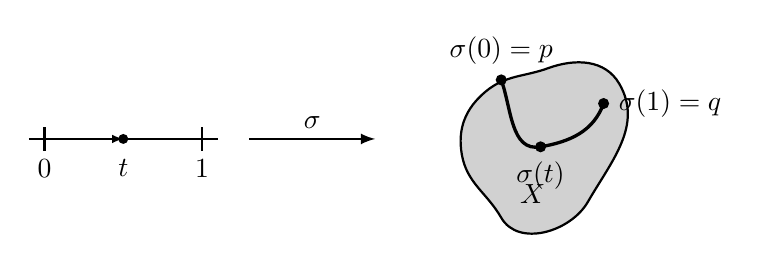
\begin{tikzpicture}[>=latex, scale=1.0]
    % Interval [0, 1]
    \draw[thick] (-0.2, 0) -- (2.2, 0);
    \draw[thick] (0, -0.15) -- (0, 0.15) node[below=8pt] {$0$};
    \draw[thick] (2.0, -0.15) -- (2.0, 0.15) node[below=8pt] {$1$};
    \fill (1.0, 0) circle (1.8pt);
    \draw[->] (0.7, 0) -- (1.0, 0);
    \node[below=4pt] at (1.0, 0) {$t$};

    % Arrow sigma
    \draw[->, thick] (2.6, 0) -- node[above] {$\sigma$} (4.2, 0);

    % Set X
    \begin{scope}[shift={(5.6, 0)}]
      \def\xshape{(0, 0.6) to[out=40, in=-160] (0.8, 0.9)
                  to[out=20, in=120] (1.7, 0.7)
                  to[out=-60, in=60] (1.3, -0.8)
                  to[out=-120, in=-60] (0.2, -1.0)
                  to[out=120, in=-80] (-0.3, -0.2)
                  to[out=100, in=-140] (0, 0.6)}
      \fill[black!18] \xshape;
      \draw[thick] \xshape;
      \node at (0.6, -0.7) {$X$};

      % Curve sigma(t)
      \coordinate (P) at (0.2, 0.75);
      \coordinate (Q) at (1.5, 0.45);
      \draw[very thick] (P) to[out=-70, in=-170] (0.7, -0.1)
                           to[out=10, in=-110] (Q);
      \fill (P) circle (2pt) node[above=2pt] {$\sigma(0)=p$};
      \fill (Q) circle (2pt) node[right=2pt] {$\sigma(1)=q$};
      \coordinate (Pt) at (0.7, -0.1);
      \fill (Pt) circle (2pt);
      \node[below=2pt] at (Pt) {$\sigma(t)$};
    \end{scope}
  \end{tikzpicture}
  \caption{道路连通示意图}\label{fig:7.2.2}
\end{figure}

应该注意的是, 道路指的是连续映射 $\sigma$, 而不是 $\sigma$ 的像 $\sigma([0,1]) = \{\sigma(t) \mid t \in [0,1]\}$.

\begin{example}\label{ex:7.2.2}
设 $X$ 为 $\mathbb{R}^n$ 中的一个凸集, 即 $\forall p, q \in X, \forall t \in [0,1]$, 必有 $(1-t)p + tq \in X$, 则 $X$ 作为通常的 Euclid 空间 $(\mathbb{R}^n, \mathcal{T}_{\rho_0}^n)$ 的子拓扑空间是道路连通的. 事实上, 只需取连接 $p$ 与 $q$ 的道路为 $\sigma\colon [0,1] \to X, \sigma(t) = (1-t)p + tq$ (\cref{fig:7.2.3}).

显然, 直线上的 (开或闭或半开半闭) 区间, 平面上的 (开或闭) 圆片 (椭圆片), $\mathbb{R}^{n} (n \geqslant 3)$ 中的 (开或闭) 球体 (椭球体), 还有 $\mathbb{R}^{n} (n \geqslant 1)$ 本身都是凸集. 因而, 它们都是道路连通的.

考察平面上的集合
\[
  X = [-2, 2] \times [-1, 0] \cup [-2, -1] \times [0, 1] \cup [1, 2] \times [0, 1],
\]
它是道路连通的, 但不是凸集 (\cref{fig:7.2.4}).
\end{example}

\begin{figure}[htbp]
  \centering
  \begin{minipage}[b]{0.45\linewidth}
    \centering
    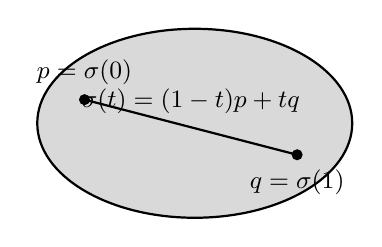
\begin{tikzpicture}[>=latex, scale=1.0]
      % Convex ellipse
      \fill[black!15] (0, 0) ellipse (2.0 and 1.2);
      \draw[thick] (0, 0) ellipse (2.0 and 1.2);

      \coordinate (p) at (-1.4, 0.3);
      \coordinate (q) at (1.3, -0.4);
      \draw[thick] (p) -- node[above=1pt] {\small $\sigma(t)=(1-t)p+tq$} (q);
      \fill (p) circle (2pt) node[above=2pt] {\small $p=\sigma(0)$};
      \fill (q) circle (2pt) node[below=2pt] {\small $q=\sigma(1)$};
    \end{tikzpicture}
    \caption{凸集是道路连通的}\label{fig:7.2.3}
  \end{minipage}\qquad
  \begin{minipage}[b]{0.48\linewidth}
    \centering
    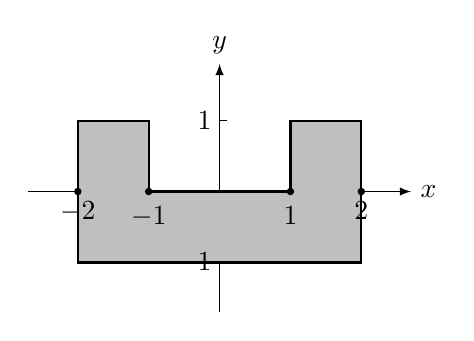
\begin{tikzpicture}[>=latex, scale=0.9]
      % Axes
      \draw[->] (-2.7, 0) -- (2.7, 0) node[right] {$x$};
      \draw[->] (0, -1.7) -- (0, 1.8) node[above] {$y$};
      \node[below left] at (0, 0) {$O$};

      % Set X shaded
      \fill[black!25] (-2, -1) rectangle (2, 0);
      \fill[black!25] (-2, 0) rectangle (-1, 1);
      \fill[black!25] (1, 0) rectangle (2, 1);

      % Boundary of X
      \draw[thick] (-2, 0) -- (-2, 1) -- (-1, 1) -- (-1, 0) -- (1, 0) -- (1, 1) -- (2, 1) -- (2, -1) -- (-2, -1) -- cycle;

      % Ticks & labels
      \draw (0, 1) -- (0.1, 1) node[left=2pt] {$1$};
      \draw (0, -1) -- (0.1, -1) node[left=2pt] {$-1$};
      \fill (-2, 0) circle (1.5pt) node[below] {$-2$};
      \fill (-1, 0) circle (1.5pt) node[below=2pt] {$-1$};
      \fill (1, 0) circle (1.5pt) node[below=2pt] {$1$};
      \fill (2, 0) circle (1.5pt) node[below] {$2$};
    \end{tikzpicture}
    \caption{道路连通但非凸集}\label{fig:7.2.4}
  \end{minipage}
\end{figure}

\begin{definition}\label{def:7.2.3}
设 $(X, \mathcal{T})$ 为拓扑空间, 如果 $X$ 为两个不相交的非空开集的并, 则称 $(X, \mathcal{T})$ 为\textbf{非连通的拓扑空间}, 否则称为\textbf{连通的拓扑空间}.
\end{definition}

易见:
\begin{align*}
  X \text{ 非连通} &\iff X \text{ 为两个不相交的非空闭集的并} \\
  &\iff X \text{ 含有一个非空的真子集, 它既为开集又为闭集}.
\end{align*}

\begin{example}\label{ex:7.2.3}
$[a,b]$ ($a<b, a, b \in \mathbb{R}$) 作为 $(\mathbb{R}^{1}, \mathcal{T}_{\rho_{0}}^{1})$ 的子拓扑空间是连通的.
\end{example}

\begin{proof}
(反证) 假设 $[a,b]$ 非连通, 则 $[a,b] = U \cup V$, $U$ 与 $V$ 为 $[a,b]$ 中不相交的非空开集. 取 $p \in U, q \in V$, 不妨设 $p < q$. 令
\[
  \xi = \sup\{x \mid x \in U \cap [p,q]\}.
\]
由 $U$ 与 $V$ 为开集, 易见 $p < \xi < q$. 再由 $\sup$ 的定义知 $\xi \notin V \cap [p, q]$, 而由 $(\xi, q) \subset V$ 知 $\xi \notin U \cap [p, q]$. 因此,
\[
  \xi \notin (U \cap [p,q]) \cup (V \cap [p,q]) = (U \cup V) \cap [p,q] = [p,q],
\]
这与 $\xi \in [p, q]$ 相矛盾.

类似可证 $(a,b)$, $[a,b)$, $(a,b]$, $(-\infty, a)$, $(-\infty, a]$, $[a, +\infty)$, $(a, +\infty)$, $(-\infty, +\infty)$ 都是连通的.
\end{proof}

\begin{theorem}\label{thm:7.2.5}
拓扑空间 $(X, \mathcal{T})$ 道路连通必连通, 但反之不真.
\end{theorem}

\begin{proof}
(反证) 假设 $(X, \mathcal{T})$ 非连通, 则 $X = U \cup V$, $U$ 与 $V$ 为 $(X, \mathcal{T})$ 中的非空不相交的开集. 取 $p \in U, q \in V$, 显然 $p \neq q$. 因 $(X, \mathcal{T})$ 道路连通, 故存在连接 $p$ 与 $q$ 的道路 $\sigma\colon [0,1] \to X$, 使 $\sigma(0) = p \in U, \sigma(1) = q \in V$. 于是,
\[
  [0,1] = \sigma^{-1}(X) = \sigma^{-1}(U \cup V) = \sigma^{-1}(U) \cup \sigma^{-1}(V),
\]
其中 $0 \in \sigma^{-1}(U), 1 \in \sigma^{-1}(V)$. 由 $\sigma$ 连续知 $\sigma^{-1}(U)$ 与 $\sigma^{-1}(V)$ 为 $[0,1]$ 的不相交的非空开集, 从而 $[0,1]$ 非连通, 这与\cref{ex:7.2.3}中的结论相矛盾.

反之不真, 参阅\cref{ex:7.2.5}与\cref{ex:7.2.6}.
\end{proof}

\cref{thm:7.2.5}与\cref{ex:7.2.2}表明, $(\mathbb{R}^{n}, \mathcal{T}_{\rho_{0}^{n}})$ 中的任何凸集都是道路连通的, 因而也是连通的.

\begin{example}\label{ex:7.2.4}
设 $A$ 为平面 $(\mathbb{R}^2, \mathcal{T}_{\rho_0}^2)$ 中的至多可数集, 则 $\mathbb{R}^2 \setminus A$ 为 $(\mathbb{R}^2, \mathcal{T}_{\rho_0}^2)$ 的道路连通子集, 当然也是连通子集.
\end{example}

\begin{proof}
$\forall p, q \in \mathbb{R}^2 \setminus A, p \neq q$. 作线段 $\overline{pq}$ 的垂直平分线 $l$, 再过 $p, q$ 并以 $\overline{pq}$ 为弦作圆弧, 则必有一条圆弧 $\overset{\frown}{prq} \subset \mathbb{R}^2 \setminus A$ (如\cref{fig:7.2.5}, 因 $A$ 为至多可数集, $l$ 上的点不可数, 故圆弧为不可数集), 它就是 $\mathbb{R}^2 \setminus A$ 中连接 $p$ 与 $q$ 的一条道路, 从而, $\mathbb{R}^2 \setminus A$ 是道路连通的. 再根据\cref{thm:7.2.5}, $\mathbb{R}^2 \setminus A$ 也是连通的.
\end{proof}

\begin{figure}[htbp]
  \centering
  \begin{tikzpicture}[>=latex, scale=1.0]
    % Axes
    \draw[->] (-0.3, 0) -- (4.2, 0) node[right] {$x$};
    \draw[->] (0, -0.3) -- (0, 2.5) node[above] {$y$};
    \node[below left] at (0, 0) {$O$};

    % Points p and q
    \coordinate (p) at (0.4, 0.4);
    \coordinate (q) at (3.5, 1.0);
    \fill (p) circle (2pt) node[below=2pt] {$p$};
    \fill (q) circle (2pt) node[right=2pt] {$q$};

    % Straight line pq (for construction)
    \draw[thick] (p) -- (q);

    % Midpoint and perpendicular bisector l
    \coordinate (m) at ($(p)!0.5!(q)$);
    \draw[thick] (1.3, 2.2) -- (2.3, -0.2) node[right] {$l$};

    % Circular arc prq
    \draw[very thick] (p) to[out=60, in=165] (1.8, 1.6) to[out=-15, in=140] (q);
    \coordinate (r) at (1.8, 1.6);
    \fill (r) circle (2pt) node[above=2pt] {$r$};
  \end{tikzpicture}
  \caption{$\mathbb{R}^2 \setminus A$ 的圆弧道路}\label{fig:7.2.5}
\end{figure}

\begin{theorem}\label{thm:7.2.6}
设 $(X, \mathcal{T})$ 为拓扑空间, $Y$ 为 $(X, \mathcal{T})$ 的连通子集 (即 $Y$ 作为子拓扑空间是连通的), 且 $Y \subset Z \subset \overline{Y}$, 则 $Z$ 也连通. 特别地, $\overline{Y}$ 是连通的.
\end{theorem}

\begin{proof}
(反证) 假设 $Z$ 非连通, 则 $Z = A \cup B$, $A$ 与 $B$ 为 $Z$ 中不相交的非空开集. 因为连通子集 $Y = (Y \cap A) \cup (Y \cap B)$, 而 $Y \cap A$ 与 $Y \cap B$ 为 $Y$ 中的开集. 所以, $Y \cap A = \varnothing$ 或 $Y \cap B = \varnothing$, 即 $Y \subset B$ 或 $Y \subset A$. 不妨设 $Y \subset A$. 由于
\[
  Z \subset \overline{Y} \subset \overline{A},
\]
故
\[
  Z \cap B \subset \overline{A} \cap B = (\overline{A} \cap Z) \cap B = A^{-} \cap B = A \cap B = \varnothing
\]
(其中 $A^{-}$ 为 $A$ 在 $Z$ 中的相对闭包). 因此, $B = Z \cap B = \varnothing$. 这与假设 $B$ 非空相矛盾.
\end{proof}

\begin{theorem}\label{thm:7.2.7}
设 $(X, \mathcal{T}_{1})$ 与 $(Y, \mathcal{T}_{2})$ 都为拓扑空间, $f\colon X \to Y$ 为连续映射.
\begin{enumerate}
  \item 如果 $(X, \mathcal{T}_{1})$ 连通, 则 $f(X)$ 也连通;
  \item 如果 $(X, \mathcal{T}_{1})$ 道路连通, 则 $f(X)$ 也道路连通.
\end{enumerate}
\end{theorem}

\begin{proof}
(1) (反证) 假设 $f(X)$ 非连通, 则 $f(X) = A \cup B$, 其中 $A$ 与 $B$ 为 $f(X)$ 中的非空不相交的开子集. 由 $f$ 连续及\cref{thm:7.2.2}知, $f^{-1}(A)$ 与 $f^{-1}(B)$ 也为 $X$ 的非空不相交的开子集, 且 $X = f^{-1}(A) \cup f^{-1}(B)$, 从而 $X$ 非连通. 这与已知 $X$ 连通相矛盾. 所以, $f(X)$ 也是连通的.

(2) 设 $p, q \in f(X)$, 则 $\exists a, b \in X$, s.t. $f(a) = p, f(b) = q$. 因为 $(X, \mathcal{T}_1)$ 道路连通, 所以有连续映射 $\eta\colon [0, 1] \to X$, 使 $\eta(0) = a, \eta(1) = b$. 于是,
\[
  \sigma = f \circ \eta\colon [0, 1] \to f(X),
\]
\[
  \sigma(0) = f \circ \eta(0) = f(a) = p, \quad \sigma(1) = f \circ \eta(1) = f(b) = q
\]
为 $f(X)$ 中连接 $p$ 与 $q$ 的一条道路, 因此, $f(X)$ 是道路连通的.
\end{proof}

从\cref{thm:7.2.7}可知, 连通与道路连通都是拓扑不变性质.

\begin{example}\label{ex:7.2.5}
设
\[
  A = \left\{(x,y) \;\middle|\; y = \sin\frac{1}{x}, \; 0 < x \leqslant \frac{2}{\pi}\right\} \subset \mathbb{R}^{2}, \quad B = \left\{(0,y) \;\middle|\; -1 \leqslant y \leqslant 1\right\} \subset \mathbb{R}^{2}.
\]
显然, $\overline{A} = A \cup B$.

因为 $A$ 为 $\left(0, \frac{2}{\pi}\right]$ 的连续像, 根据\cref{thm:7.2.7}(2), $A$ 是道路连通的, 当然也是连通的, 再由\cref{thm:7.2.6}, $\overline{A}$ 是连通的, 但 $\overline{A}$ 不是道路连通的. 事实上, 设 $a \in A, b \in B, \sigma\colon [0,1] \to \overline{A}$ 为任一映射, 使得 $\sigma(0) = a, \sigma(1) = b$, 则 $\sigma$ 必不连续 (\cref{fig:7.2.6}).
\end{example}

\begin{proof}
(反证) 假设 $\sigma(t) = (x(t), y(t))$ 连续, 即 $x(t)$ 与 $y(t)$ 均连续. 令
\[
  t_{*} = \inf\{t \in [0,1] \mid \sigma(t) \in B\}.
\]
显然, $0 < t_{*}$. 由 $t_{*}$ 的定义, 存在 $t_{n} \to t_{*}^{+} (n \to +\infty)$, $\sigma(t_{n}) \in B$. 于是,
\[
  \lim_{t \to t_{*}} x(t) = x(t_{*}) = \lim_{n \to +\infty} x(t_{n}) = \lim_{n \to +\infty} 0 = 0,
\]
\[
  y(t_{*}) = \lim_{t \to t_{*}^{-}} y(t) = \lim_{t \to t_{*}^{-}} \sin\frac{1}{x(t)}.
\]
易见, 上式左边 $y(t_{*})$ 为一确定实数, 而右边由于 $\lim\limits_{t \to t_{*}^{-}} x(t) = 0$ 而无极限, 矛盾.
\end{proof}

\begin{figure}[htbp]
  \centering
  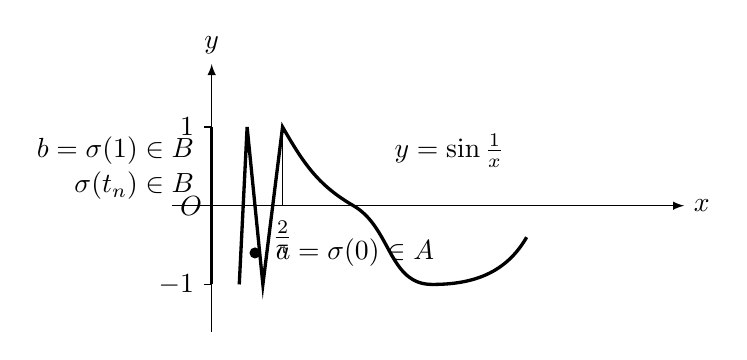
\begin{tikzpicture}[>=latex, scale=1.0]
    % Axes
    \draw[->] (-0.5, 0) -- (6.0, 0) node[right] {$x$};
    \draw[->] (0, -1.6) -- (0, 1.8) node[above] {$y$};
    \node[left] at (0, 0) {$O$};
    \draw (0, 1) -- (-0.1, 1) node[left] {$1$};
    \draw (0, -1) -- (-0.1, -1) node[left] {$-1$};

    % Sine curve: y = sin(1/x)
    \draw[very thick] (0.35, -1.0) -- (0.45, 1.0) -- (0.65, -1.0) -- (0.9, 1.0)
                      to[out=-60, in=150] (1.8, 0)
                      to[out=-30, in=180] (2.8, -1.0)
                      to[out=0, in=-120] (4.0, -0.4);
    
    % Peak at 2/pi
    \coordinate (peak) at (0.9, 1.0);
    \draw[thin] (peak) -- (0.9, 0) node[below=2pt] {$\frac{2}{\pi}$};
    \node[right] at (2.2, 0.7) {$y = \sin \frac{1}{x}$};

    % Limit segment x=0, y in [-1, 1]
    \draw[very thick] (0, -1) -- (0, 1);

    % Points a in A and b in B
    \coordinate (ptA) at (0.55, -0.6);
    \fill (ptA) circle (2pt) node[right=4pt] {$a = \sigma(0) \in A$};

    \node[left] at (-0.1, 0.7) {$b = \sigma(1) \in B$};
    \node[left] at (-0.1, 0.25) {$\sigma(t_n) \in B$};
  \end{tikzpicture}
  \caption{拓扑学家的正弦曲线示意图}\label{fig:7.2.6}
\end{figure}

\begin{example}\label{ex:7.2.6}
设 $\mathbb{R}_{+}^{2} = \{(x,y) \in \mathbb{R}^{2} \mid y > 0\} = (-\infty, +\infty) \times (0, +\infty)$,
\[
  F_{n} = [-n, n] \times \left[\frac{1}{n} - \frac{1}{4n(n+1)}, \; \frac{1}{n} + \frac{1}{4n(n+1)}\right], \quad n = 1, 2, \cdots,
\]
则:
\begin{enumerate}
  \item $G = \mathbb{R}_+^2 \setminus \bigcup\limits_{n=1}^{\infty} F_n$ 为开区域 (连通的开集称为开区域);
  \item $G$ 的闭包 $\overline{G}$ 为 $(\mathbb{R}^{2}, \mathcal{T}_{\rho_{0}}^{2})$ 的连通子集;
  \item $\overline{G}$ 在 $(\mathbb{R}^{2}, \mathcal{T}_{\rho_{0}}^{2})$ 中不是道路连通的.
\end{enumerate}
\end{example}

\begin{proof}
(1) $\forall p \in G$, 显然 $\varepsilon = \rho_{0}^{2}(p, G^{c}) = \inf\limits_{q \in G^{c}} \rho_{0}^{2}(p,q) > 0$, 则以 $p$ 为中心 $\varepsilon$ 为半径的开圆片 $B(p; \varepsilon) \subset G$. 因此, $G$ 为开集.

设 $p, q \in G, p \neq q$, 显然在 $G$ 中存在折线 (由平行于坐标轴的直线段组成) 将 $p$ 与 $q$ 相连接. 因此, $G$ 是折线连通的, 当然是道路连通的. 根据\cref{thm:7.2.5}知, 它也是连通的. 这就证明了 $G$ 为连通的开集, 即 $G$ 为开区域.

(2) 由\cref{thm:7.2.6}推得 $\overline{G}$ 是连通的.

(3) (反证) 假设 $\overline{G}$ 是道路连通的, 则对 $(0,0) \in \overline{G}, (0,2) \in \overline{G}$, 必有连接 $(0,0)$ 与 $(0,2)$ 的一条道路, 即存在连续映射
\[
  \sigma\colon [0,1] \to \overline{G}, \quad \sigma(t) = (x(t), y(t)), \quad \sigma(0) = (0,0), \quad \sigma(1) = (0,2),
\]
其中 $x(t), y(t)$ 均为 $t$ 的连续函数 (\cref{fig:7.2.7}). 由一元连续函数的最值定理, $\exists t_{*} \in [0,1]$, s.t. $|x(t_{*})| = \max\limits_{t \in [0,1]} |x(t)|$. 取 $N \in \mathbb{Z}_{+}$, s.t. $N > |x(t_{*})|$. 由于 $0 < \frac{1}{N} < 2$ 和一元连续函数的介值定理, $\exists t_{**} \in (0,1)$, s.t. $y(t_{**}) = \frac{1}{N}$. 所以
\begin{align*}
  (x(t_{**}), y(t_{**})) &= \left(x(t_{**}), \frac{1}{N}\right) \in \left([-|x(t_{*})|, |x(t_{*})|] \times \left\{\frac{1}{N}\right\}\right) \cap \overline{G} \\
  &\subset \left((-N, N) \times \left\{\frac{1}{N}\right\}\right) \cap \overline{G} = \varnothing,
\end{align*}
矛盾. 从而 $\overline{G}$ 不是道路连通的.
\end{proof}

\begin{figure}[htbp]
  \centering
  \begin{tikzpicture}[>=latex, scale=1.0]
    % Axes
    \draw[->] (-2.5, 0) -- (3.5, 0) node[right] {$x$};
    \draw[->] (0, -0.5) -- (0, 2.6) node[above] {$y$};
    \node[below right] at (0, 0) {$O$};

    % Ticks on x
    \draw (-2, 0) -- (-2, -0.1) node[below] {$-2$};
    \draw (-1, 0) -- (-1, -0.1) node[below] {$-1$};
    \draw (1, 0) -- (1, -0.1) node[below] {$1$};
    \draw (2, 0) -- (2, -0.1) node[below] {$2$};

    % Horizontal strips at heights 1/N, 1/2, 1
    % Height 1/N (black filled strip)
    \fill[black] (-2.5, 0.15) rectangle (2.5, 0.3);
    \draw[thick] (-2.5, 0.15) rectangle (2.65, 0.3);
    \draw (0, 0.22) -- (-0.1, 0.22) node[left=1pt] {$\frac{1}{N}$};

    % Height 1/2 (shaded strip)
    \fill[black!30] (-2, 0.45) rectangle (2.2, 0.6);
    \draw[thick] (-2, 0.45) rectangle (2.2, 0.6);
    \draw (0, 0.52) -- (-0.1, 0.52) node[left=1pt] {$\frac{1}{2}$};

    % Height 1 (hatched strip)
    \fill[pattern=north east lines, pattern color=black!70] (-1, 0.9) rectangle (1.2, 1.2);
    \draw[thick] (-1, 0.9) rectangle (1.2, 1.2);
    \draw (0, 1.05) -- (-0.1, 1.05) node[left=1pt] {$1$};

    \draw (0, 2) -- (-0.1, 2) node[left=1pt] {$2$};

    % Path from y=2 descending to strip 1/N
    \coordinate (start) at (0, 2.0);
    \draw[very thick, ->] (start) to[out=0, in=120] (0.8, 1.6)
                                 to[out=-60, in=170] (1.8, 1.4)
                                 to[out=-10, in=90] (2.4, 0.45);
    \draw[very thick, ->] (2.4, 0.45) to[out=-90, in=0] (1.5, 0.1)
                                     to[out=180, in=-20] (0, 0);

    % Pointer label
    \draw[<-] (2.45, 0.25) -- (2.8, 0.5) node[right] {$\left(x(t_{**}), \frac{1}{N}\right)$};
    \draw[<-] (2.45, 0.4) -- (2.8, 0.9) node[right] {$(x(t_*), y(t_*))$};
    \draw (2.45, 0.1) -- (2.45, -0.1) node[below] {$|x(t_*)|$};
  \end{tikzpicture}
  \caption{闭梳空间连通但非道路连通示意图}\label{fig:7.2.7}
\end{figure}

\begin{theorem}\label{thm:7.2.8}
设 $U$ 为 $(\mathbb{R}^{n}, \mathcal{T}_{\rho_{0}^{n}})$ 中的开集, 则以下结论等价:
\begin{enumerate}
  \item $U$ 折线连通;
  \item $U$ 道路连通;
  \item $U$ 连通.
\end{enumerate}
\end{theorem}

\begin{proof}
(1) $\Rightarrow$ (2): 因为折线道路是特殊的道路, 所以 $U$ 折线连通必为道路连通.

(2) $\Rightarrow$ (3): 由\cref{thm:7.2.5}即得结论.

(3) $\Rightarrow$ (1): 设 $U_x = \{ y \mid y \in U, \text{存在 } U \text{ 中连接 } x \text{ 与 } y \text{ 的折线} \}$, 则 $U_x$ 为 $(\mathbb{R}^n, \mathcal{T}_{\rho_0^n})$ 中的开集. 事实上, $\forall p \in U_x \subset U$, 由 $U$ 为开集, 存在 $p$ 的开球邻域 $B(p; \varepsilon) \subset U$, 而 $\forall q \in B(p; \varepsilon)$, 有直线段 $\overline{pq}$ 连接 $p$ 与 $q$. 因此, 在 $U$ 中有折线将 $x$ 与 $q$ 相连, 即 $q \in U_x$, $B(p; \varepsilon) \subset U_x$, 故 $U_x$ 为开集 (\cref{fig:7.2.8}).

易见, $U_{x_{1}}$ 与 $U_{x_{2}}$ 或者不相交, 或者重合. 并且,
\[
  U = U_{x} \cup \left(\bigcup_{y \in U \setminus U_{x}} U_{y}\right).
\]
由题设 $U$ 连通及 $U_x$ 非空 (因 $x \in U_x$) 可知 $\bigcup\limits_{y \in U \setminus U_x} U_y = \varnothing$, 从而 $U = U_x$, 明显地, $U$ 是折线连通的.
\end{proof}

\begin{figure}[htbp]
  \centering
  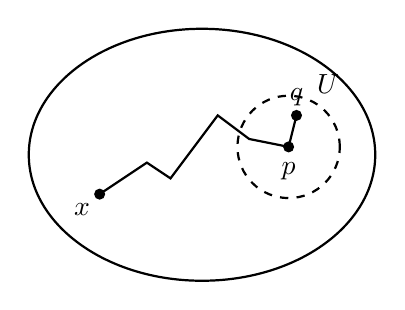
\begin{tikzpicture}[>=latex, scale=1.0]
    % Boundary of U (smooth oval)
    \draw[thick] (0, 0) circle [x radius=2.2, y radius=1.6];
    \node at (1.6, 0.9) {$U$};

    % Points x and p
    \coordinate (x) at (-1.3, -0.5);
    \coordinate (p) at (1.1, 0.1);
    \fill (x) circle (2pt) node[below left] {$x$};

    % Broken line path from x to p
    \coordinate (v1) at (-0.7, -0.1);
    \coordinate (v2) at (-0.4, -0.3);
    \coordinate (v3) at (0.2, 0.5);
    \coordinate (v4) at (0.6, 0.2);
    \draw[thick] (x) -- (v1) -- (v2) -- (v3) -- (v4) -- (p);

    % Neighborhood B(p; eps)
    \draw[dashed, thick] (p) circle (0.65);
    \fill (p) circle (2pt) node[below=2pt] {$p$};

    % Point q in B(p; eps)
    \coordinate (q) at (1.2, 0.5);
    \fill (q) circle (2pt) node[above] {$q$};
    \draw[thick] (p) -- (q);
  \end{tikzpicture}
  \caption{开集 $U$ 中的折线连通}\label{fig:7.2.8}
\end{figure}


\begin{exblock}{练习题 7.2}

  \item 设 $x^{0} \in \mathbb{R}^{n}$, 证明: $(\mathbb{R}^{n}, \mathcal{T}_{\rho_{0}^{n}})$ 中开球 $B(x^{0}; \delta)$ 为凸开集, 因而为开区域.

  \item 设 $A \subset \mathbb{R}^n$, 如果 $A$ 既为开集又为闭集, 证明: $A = \varnothing$ 或者 $A = \mathbb{R}^n$.

  \item 应用反证法及\cref{ex:7.2.3}证明 $(\mathbb{R}^{n}, \mathcal{T}_{\rho_{0}^{n}})$ 是连通的.

  \item 设 $(X, \mathcal{T})$ 连通, $\mathcal{T}' \subset \mathcal{T}$ 为 $X$ 的拓扑, 则 $(X, \mathcal{T}')$ 也是连通空间. 上述``连通''改为``道路连通''结论如何? 并说明理由.

  \item 设 $A$ 为拓扑空间 $(X, \mathcal{T})$ 的连通子集, $B$ 为 $(X, \mathcal{T})$ 的既开又闭的子集, 如果 $A \cap B \neq \varnothing$, 则 $A \subset B$.

  \item 设 $Y$ 为拓扑空间 $(X, \mathcal{T})$ 的连通子集, $Z$ 为 $X$ 的子集. 如果 $Y \cap \overline{Z} \neq \varnothing, Y \cap \overline{Z}^c \neq \varnothing$, 证明: $Y \cap \partial Z \neq \varnothing$.

  \item 设 $A$ 为连通空间 $(X, \mathcal{T})$ 的非空真子集. 证明: $\partial A \neq \varnothing$.

  \item 证明: $(\mathbb{R}^{2}, \mathcal{T}_{\rho_{0}}^{2})$ 上所有至少有一个坐标为有理数的点构成的集合是一个道路连通子集.

  \item 设 $Y$ 是拓扑空间 $(X, \mathcal{T})$ 的一个连通子集. 证明: 如果 $A$ 与 $B$ 是 $(X, \mathcal{T})$ 的两个无交开集 (闭集) 使得 $Y \subset A \cup B$, 则或者 $Y \subset A$ 或者 $Y \subset B$.

  \item 证明:
  \begin{enumerate}
    \item 从拓扑空间到平庸拓扑空间的任何映射都为连续映射;
    \item 从离散拓扑空间到拓扑空间的任何映射都为连续映射.
  \end{enumerate}

  \item 证明: $n$ 维 Euclid 空间 $(\mathbb{R}^{n}, \mathcal{T}_{\rho_{0}}^{n})$ ($n \geqslant 2$) 与 $(\mathbb{R}^{1}, \mathcal{T}_{\rho_{0}}^{1})$ 不同胚.

  \item 设连续函数 $f\colon \mathbb{R}^n \to \mathbb{R}^1$ 既取正值又取负值. 证明: 集合 $E = \{x \in \mathbb{R}^n \mid f(x) \neq 0\}$ 为非连通集.
\end{exblock}

\begin{exblock}{思考题 7.2}
  \item 设 $(X, \mathcal{T})$ 为拓扑空间. 证明: $(X, \mathcal{T})$ 非连通 $\iff X$ 中存在两个子集 $A$ 与 $B$ 是隔离的, 即

  \[
    (A \cap \overline{B}) \cup (\overline{A} \cap B) = \varnothing.
  \]

  \item 设 $Y, Z$ 都是拓扑空间 $(X, \mathcal{T})$ 的子集, 其中 $Y$ 是连通的. 证明: 如果 $Z \cap Y \neq \varnothing$ 与 $Z \cap Y^c \neq \varnothing$, 则 $Z \cap \partial Y \neq \varnothing$.

  \item 设 $Y$ 为拓扑空间 $(X, \mathcal{T})$ 的一个子集. 证明: $\overline{Y}$ 为 $(X, \mathcal{T})$ 的一个非连通子集 $\iff X$ 中存在两个非空集合 $A$ 与 $B$ 使得 $Y \subset A \cup B$, $\overline{A} \cap \overline{B} = \varnothing$, $Y \cap A \neq \varnothing$ 与 $Y \cap B \neq \varnothing$ 成立.

  \item 在 Euclid 平面 $(\mathbb{R}^{2}, \mathcal{T}_{\rho_{0}}^{2})$ 中, 令
  \[
    L_{\frac{1}{n}} = \left\{(x,y) \;\middle|\; x - \frac{1}{n}y = 0\right\} \subset \mathbb{R}^{2}, \quad n = 1, 2, \cdots,
  \]
  \[
    L_{0} = \{(0,y) \mid y \in \mathbb{R}\} \subset \mathbb{R}^{2}.
  \]
  证明: $\forall A \subset L_{0}$, 子集 $A \cup \left(\bigcup\limits_{n=1}^{\infty} L_{\frac{1}{n}}\right)$ 是连通的. 它是道路连通的吗?

  \item 设 $A$ 为单位球面 $S^{n} (n \geqslant 2)$ 的一个至多可数的子集. 证明: $S^{n} \setminus A$ 是道路连通的.

  \item 证明: $n$ 维 Euclid 空间 $\mathbb{R}^n (n \geqslant 2)$ (或 $n$ 维单位球面 $S^n (n \geqslant 1)$) 不能嵌入到实数空间 $\mathbb{R}^1$ 中去, 即不存在同胚 $f\colon \mathbb{R}^n \to f(\mathbb{R}^n) \subset \mathbb{R}^1$ (或 $f\colon S^n \to f(S^n) \subset \mathbb{R}^1$).

  \item (\textbf{粘结引理}) 设 $A$ 与 $B$ 为拓扑空间 $(X, \mathcal{T}_{1})$ 中的两个开集 (闭集), 并且 $X = A \cup B$. 又设 $(Y, \mathcal{T}_{2})$ 也为拓扑空间, $f_{1}\colon A \to Y$ 与 $f_{2}\colon B \to Y$ 都为连续映射, 且满足:
  \[
    f_{1}\big|_{A \cap B} = f_{2}\big|_{A \cap B}.
  \]
  则
  \[
    f\colon X \to Y, \quad x \mapsto f(x) = \begin{cases}
      f_{1}(x), & x \in A, \\
      f_{2}(x), & x \in B
    \end{cases}
  \]
  为一个连续映射.

  \item 设 $A$ 与 $B$ 为 $(\mathbb{R}^{n}, \mathcal{T}_{\rho_{0}^{n}})$ 中两个不相交的闭集. 证明: 存在一个连续函数 $f\colon \mathbb{R}^{n} \to \mathbb{R}^{1}$, 使得
  \[
    f\big|_{A} \equiv 1, \quad f\big|_{B} \equiv 0.
  \]
  \textit{提示}: 令 $f(x) = \frac{\rho(x, B)}{\rho(x, A) + \rho(x, B)}$, 其中 $\rho(x, A) = \inf\limits_{y \in A} \rho(x, y)$.

  \item 设 $(X,\mathcal{T}_{1})$ 与 $(Y,\mathcal{T}_{2})$ 都为拓扑空间, $f\colon X \to Y$ 为映射. 证明:
  \[
    f \text{ 为连续映射} \iff \forall A \subset X, \; f(\overline{A}) \subset \overline{f(A)}.
  \]

  \item 举出连续函数 $f\colon \mathbb{R}^1 \to \mathbb{R}^1$ 及 $A \subset \mathbb{R}^1$, 使 $f(\overline{A}) \subsetneq \overline{f(A)}$.
\end{exblock}
\section{紧致、可数紧致、列紧、序列紧致}\label{sec:7.3}

上两节介绍的 $A_{1}$, $A_{2}$, $T_{2}$, 连通性及道路连通性都是拓扑不变性, 即拓扑映射 (同胚) 下不变的性质. \cref{thm:7.2.7} 表明, 连通与道路连通还是连续不变性.

\begin{theorem}\label{thm:7.3.1}
设 $(X, \mathcal{T})$ 为拓扑空间.
\begin{enumerate}
  \item \textbf{紧致空间}: $X$ 的任何开覆盖必有有限子覆盖;

  \item \textbf{可数紧致空间}: $X$ 的任何可数开覆盖必有有限子覆盖;

  \item \textbf{列紧空间}: $X$ 的任何无限子集 $A$ 必有聚点 $a \in X$;

  \item \textbf{序列紧致空间}: $X$ 中每个点列 $\{x_{n}\}$ 必有收敛于 $x \in X$ 的子点列 $\{x_{n_{k}}\}$;

  \item 任何递降非空闭集序列 $\{F_{i}\}$ 必有交, 即 $\exists x \in \bigcap\limits_{n=1}^{\infty} F_{n}$ (或 $\bigcap\limits_{n=1}^{\infty} F_{n} \neq \varnothing$).
\end{enumerate}
它们具有如下关系:
\begin{center}
\begin{tikzpicture}[>=latex, x=1.5cm, y=1.5cm]
  \tikzset{
    node distance=0pt,
    nd/.style={inner sep=0pt, font=\normalsize},
    a/.style={line width=0.7pt, double, double distance=1.6pt, shorten <=3.5pt, shorten >=3.5pt,
              {Triangle[open, width=5pt, length=4pt]}-{Triangle[open, width=5pt, length=4pt]}},
    as/.style={line width=0.7pt, double, double distance=1.6pt, shorten <=3.5pt, shorten >=3.5pt,
               -{Triangle[open, width=5pt, length=4pt]}}
  }
  \node[nd] (n1) at (1.75, 1.75) {(1)};
  \node[nd] (n2) at (-0.25, 1.75) {(2)};
  \node[nd] (n3) at (-0.25, 0.05) {(3)};
  \node[nd] (n4) at (1.55, 0.05) {(4)};
  \node[nd] (n5) at (0.85, 0.85) {(5)};

  \draw[as] (n1) -- (n2);        % (1) => (2)
  \draw[as] (n2) -- (n3);        % (2) => (3)
  \draw[a]  (n2) -- (n5);        % (2) <=> (5)
  \draw[as] (n4) -- (n5);        % (4) => (5)
\end{tikzpicture}
\end{center}
\end{theorem}

\begin{proof}
(1) $\Rightarrow$ (2) 显然.

(2) $\Rightarrow$ (3) 设 $A$ 为 $X$ 的任一无限子集. 取 $A$ 的可数子集 $A_{1}$, 下证 $A_{1}$ 必有聚点 (属于 $X$), 当然它也是 $A$ 的聚点. (反证) 假设 $A_{1}$ 无聚点, 即 $A_{1}' = \varnothing \subset A_{1}$, 根据\cref{thm:7.1.5}(2), $A_{1}$ 为闭集. $\forall x \in A_{1}$, 由于 $x$ 不为 $A_{1}$ 的聚点, 故存在 $x$ 的开邻域 $U_{x}$, 使
\[
  U_{x} \cap (A_{1} \setminus \{x\}) = \varnothing,
\]
即
\[
  U_{x} \cap A_{1} = \{x\}.
\]
显然, $\{U_{x} \mid x \in A_{1}\} \cup \{A_{1}^{c}\}$ 为 $X$ 的可数开覆盖, 而 $(X, \mathcal{T})$ 为可数紧致空间, 故必存在有限子覆盖 $\{U_{x_{1}}, U_{x_{2}}, \cdots, U_{x_{n}}, A_{1}^{c}\}$. 因为 $A_{1}^{c}$ 中无 $A_{1}$ 的点, 所以 $\{U_{x_{1}}, U_{x_{2}}, \cdots, U_{x_{n}}\}$ 覆盖 $A_{1}$, 从而
\[
  A_{1} = \left(\bigcup_{i=1}^{n} U_{x_{i}}\right) \cap A_{1} = \bigcup_{i=1}^{n} \left(U_{x_{i}} \cap A_{1}\right) = \{x_{1}, x_{2}, \cdots, x_{n}\}
\]
为有限集, 这与 $A_{1}$ 为可数集相矛盾.

(2) $\Rightarrow$ (5) (反证) 假设 $\bigcap\limits_{n=1}^{\infty} F_{n} = \varnothing$, 则由 De Morgan 公式, 有
\[
  \bigcup_{n=1}^{\infty} F_{n}^{c} = \left(\bigcap_{n=1}^{\infty} F_{n}\right)^{c} = \varnothing^{c} = X.
\]
因此, $\{F_{n}^{c} \mid n \in \mathbb{Z}_{+}\}$ 为 $X$ 的可数开覆盖. 由 (2), 存在有限子覆盖 $\{F_{n_{1}}^{c}, F_{n_{2}}^{c}, \cdots, F_{n_{k}}^{c}\}$. 于是, 由
\[
  F_{n_{1}}^{c} \cup F_{n_{2}}^{c} \cup \cdots \cup F_{n_{k}}^{c} = X
\]
推出
\[
  \begin{aligned}
    \varnothing \neq F_{\max\{n_{1}, n_{2}, \cdots, n_{k}\}} &= F_{n_{1}} \cap F_{n_{2}} \cap \cdots \cap F_{n_{k}} \reason{De Morgan 公式} \left(F_{n_{1}}^{c} \cup F_{n_{2}}^{c} \cup \cdots \cup F_{n_{k}}^{c}\right)^{c} \\
    &= X^{c} = \varnothing.
  \end{aligned}
\]
矛盾. 所以, $\bigcap\limits_{n=1}^{\infty} F_{n} \neq \varnothing$.

(2) $\Leftrightarrow$ (5) 设 $\mathcal{I} = \{U_{n} \mid n \in \mathbb{Z}_{+}\}$ 为 $X$ 的任一可数开覆盖, 我们断定 $\mathcal{I}$ 必有有限子覆盖. (反证) 假设 $\mathcal{I}$ 无有限子覆盖. 令
\[
  F_{n} = \left(\bigcup_{i=1}^{n} U_{i}\right)^{c}, \quad n \in \mathbb{Z}_{+},
\]
则 $F_{n} \neq \varnothing$ (由 $\bigcup\limits_{i=1}^{n} U_{i} \neq X$), 且
\[
  F_{1} \supseteq F_{2} \supseteq \cdots \supseteq F_{n} \supseteq \cdots,
\]
由 (5) 得到
\[
  \varnothing \neq \bigcap_{n=1}^{\infty} F_{n} = \bigcap_{n=1}^{\infty} \left(\bigcup_{i=1}^{n} U_{i}\right)^{c} = \left(\bigcup_{n=1}^{\infty} \left(\bigcup_{i=1}^{n} U_{i}\right)\right)^{c} = \left(\bigcup_{n=1}^{\infty} U_{n}\right)^{c} = X^{c} = \varnothing,
\]
矛盾. 从而 $\mathcal{I}$ 有有限子覆盖, $(X, \mathcal{T})$ 是可数紧致的.

(4) $\Rightarrow$ (5) $\Leftrightarrow$ (2) 设 $\{F_{n}\}$ 为 $(X, \mathcal{T})$ 中任一递降非空闭集序列, 取 $x_{n} \in F_{n}$, $n \in \mathbb{Z}_{+}$, 因为 $X$ 是序列紧致的, 故存在 $\{x_{n}\}$ 的子点列 $\{x_{n_{i}}\}$ 收敛于 $x \in X$. 由于 $x_{n_{j}} \in F_{n_{i}}$ ($j = i, i+1, \cdots$), 以及 $F_{n_{i}}$ 为闭集, 所以, $x \in F_{n_{i}} \subset F_{i}$ ($i \in \mathbb{Z}_{+}$), 从而 $x \in \bigcap\limits_{n=1}^{\infty} F_{n}$. 这就证明了 $\bigcap\limits_{n=1}^{\infty} F_{n} \neq \varnothing$, (5) 成立.
\end{proof}

\begin{theorem}\label{thm:7.3.2}
对于度量空间 $(X, \rho)$ 诱导的拓扑空间 $(X, \mathcal{T}_{\rho})$, 关于\cref{thm:7.3.1}中的 (1)$\sim$(5), 有如下关系:
\begin{center}
\begin{tikzpicture}[>=latex, x=1.5cm, y=1.5cm]
  \tikzset{
    nd/.style={inner sep=0pt, font=\normalsize},
    a/.style={line width=0.7pt, double, double distance=1.6pt, shorten <=3.5pt, shorten >=3.5pt,
              {Triangle[open, width=5pt, length=4pt]}-{Triangle[open, width=5pt, length=4pt]}},
    as/.style={line width=0.7pt, double, double distance=1.6pt, shorten <=3.5pt, shorten >=3.5pt,
               -{Triangle[open, width=5pt, length=4pt]}}
  }
  \node[nd] (n1) at (1.75, 1.75) {(1)};
  \node[nd] (n2) at (-0.25, 1.75) {(2)};
  \node[nd] (n3) at (-0.25, 0.05) {(3)};
  \node[nd] (n4) at (1.75, 0.05) {(4)};
  \node[nd] (n5) at (0.75, 0.85) {(5)};

  \draw[a]  (n1) -- (n2);        % (1) <=> (2)
  \draw[as] (n2) -- (n3);        % (2) => (3)
  \draw[a]  (n2) -- (n5);        % (2) <=> (5)
  \draw[as] (n3) -- (n5);        % (3) => (5)
  \draw[as] (n3) -- (n4);        % (3) => (4)
  \draw[as] (n4) -- (n5);        % (4) => (5)
  \draw[as] (n4) -- (n1);        % (4) => (1)
\end{tikzpicture}
\end{center}
\end{theorem}

\begin{proof}
由\cref{thm:7.3.1}, 只需证明:

(3) $\Rightarrow$ (4) 设 $\{x_{n}\}$ 为 $(X, \mathcal{T}_{\rho})$ 中任一点列, 记 $A = \{x_{n} \mid n \in \mathbb{Z}_{+}\}$.

如果 $A$ 为有限集, 则 $\exists x \in A$, $n_{1} < n_{2} < \cdots < n_{k} < \cdots$, s. t. $x_{n_{k}} = x$. 于是
\[
  \lim_{k \to +\infty} x_{n_{k}} = x \in X.
\]
如果 $A$ 为无限集, 由于 $(X, \mathcal{T}_{\rho})$ 为列紧空间, $\exists x \in A'$. 令
\[
  A_{n} = \{x_{n}, x_{n+1}, \cdots\},
\]
\[
  n_{1} = \min\{j \mid x_{j} \in B(x; 1) \cap A_{1}\},
\]
\[
  n_{2} = \min\left\{j \;\middle|\; x_{j} \in B\left(x; \frac{1}{2}\right) \cap A_{n_{1}+1}\right\},
\]
\[
  \qquad \vdots
\]
\[
  n_{k} = \min\left\{j \;\middle|\; x_{j} \in B\left(x; \frac{1}{k}\right) \cap A_{n_{k-1}+1}\right\},
\]
\[
  \qquad \vdots
\]
显然, $x_{n_{k-1}} \notin A_{n_{k-1}+1}$, $n_{1} < n_{2} < \cdots < n_{k} < \cdots$, 从而 $\{x_{n_{k}}\}$ 为 $\{x_{n}\}$ 的一个子点列, 且 $x_{n_{k}} \in B\left(x; \frac{1}{k}\right)$, $0 \leqslant \rho\left(x_{n_{k}}, x\right) < \frac{1}{k} \to 0$ ($k \to +\infty$), 即 $\lim\limits_{k \to +\infty} x_{n_{k}} = x$. 这就证明了 $(X, \mathcal{T}_{\rho})$ 是序列紧致的.

(4) $\Rightarrow$ (1) 设 $(X, \rho)$ 为序列紧致的度量空间, $\mathcal{I}$ 为 $X$ 的一开覆盖, 根据\cref{thm:7.4.4} (Lebesgue 数定理), 有 Lebesgue 数 $\lambda = \lambda(\mathcal{I}) > 0$. 令
\[
  \widetilde{\mathcal{I}} = \left\{B\left(x; \frac{\lambda}{3}\right) \;\middle|\; x \in X\right\},
\]
则开覆盖 $\widetilde{\mathcal{I}}$ 有有限子覆盖. (反证) 假设 $\widetilde{\mathcal{I}}$ 无有限子覆盖, 则 $\widetilde{\mathcal{I}}$ 的任何有限子族都不覆盖 $X$. 任取 $x_{1} \in X$, 因为 $\left\{B\left(x_{1}; \frac{\lambda}{3}\right)\right\}$ 不是 $X$ 的覆盖, 取 $x_{2} \in X \setminus B\left(x_{1}; \frac{\lambda}{3}\right)$. 假定已定义了 $x_{1}, x_{2}, \cdots, x_{n} \in X$ 满足: 若 $j > i$, 则 $x_{j} \notin B\left(x_{i}; \frac{\lambda}{3}\right)$ (即 $\rho\left(x_{i}, x_{j}\right) > \frac{\lambda}{3}$)$^{(*)}$. 由于
\[
  \left\{B\left(x_{1}; \frac{\lambda}{3}\right), B\left(x_{2}; \frac{\lambda}{3}\right), \cdots, B\left(x_{n}; \frac{\lambda}{3}\right)\right\}
\]
不是 $X$ 的覆盖, 故可取
\[
  x_{n+1} \in X \setminus \bigcup_{i=1}^{n} B\left(x_{i}; \frac{\lambda}{3}\right).
\]
易见, $x_{1}, x_{2}, \cdots, x_{n+1}$ 也满足 $^{(*)}$. 因此, 我们归纳定义了 $X$ 中的一个序列 $\{x_{n}\}$ 满足 $^{(*)}$. 可以断定 $\{x_{n}\}$ 无收敛子序列 (否则, 若有子序列收敛于 $x$, 则 $B\left(x; \frac{\lambda}{6}\right)$ 中必含 $\{x_{n}\}$ 的无限多个点, 这是不可能的. 因为 $\{x_{n}\}$ 中不同点的距离大于 $\frac{\lambda}{3}$, 但 $B\left(x; \frac{\lambda}{6}\right)$ 中任意两点的距离都小于 $\frac{\lambda}{3}$), 这与 $(X, \mathcal{T}_{\rho})$ 为序列紧致空间相矛盾. 这证明了 $\widetilde{\mathcal{I}}$ 有有限子覆盖.

设 $\widetilde{\mathcal{I}}$ 的有限子覆盖为 $\left\{B\left(y_{1}; \frac{\lambda}{3}\right), B\left(y_{2}; \frac{\lambda}{3}\right), \cdots, B\left(y_{n}; \frac{\lambda}{3}\right)\right\}$, 由 $\forall i, \exists A_{i} \in \mathcal{I}$, s.t. $B\left(y_{i}; \frac{\lambda}{3}\right) \subset A_{i}$. 易见, $\{A_{1}, A_{2}, \cdots, A_{n}\}$ 为 $\mathcal{I}$ 的有限子覆盖. 于是证明了 $(X, \mathcal{T}_{\rho})$ 为紧致空间.
\end{proof}

\begin{theorem}\label{thm:7.3.3}
在 $(X, \mathcal{T}_{\rho})$ 中, 如果 $A \subset X$ (作为子拓扑空间) 序列紧致 (或可数紧致或列紧或紧致), 则 $A$ 为 $(X, \mathcal{T}_{\rho})$ 中的有界闭集. 但反之不真.
\end{theorem}

\begin{proof}[证法 1]
(反证) 假设 $A$ 无界, 则 $\exists x_{n}, x_{0} \in A$, s. t. $\rho(x_{n}, x_{0}) \geqslant n$. 显然, $\{x_{n}\}$ 无收敛子列. 这与 $A$ 序列紧致相矛盾. 因此, $A$ 有界.

(反证) 假设 $A$ 不为闭集, 则 $\exists x_{n} \in A$, 它收敛于 $x$, 但 $x \notin A$. 当然, $\{x_{n}\}$ 的一切子列也收敛于 $x \notin A$. 从而 $A$ 不是序列紧致的, 这与已知 $A$ 序列紧致相矛盾. 因此, $A$ 为闭集.

进而, 根据\cref{thm:7.3.2}, 可数紧致或列紧或紧致必为序列紧致, 因此, 也能推得 $A$ 为 $(X, \mathcal{T}_{\rho})$ 中的有界闭集.
\end{proof}

如果 $(X, \mathcal{T}_{\rho})$ 紧致, 我们还有下面两个证法.

\begin{proof}[证法 2]
取一定点 $x \in A$. 显然, $\mathcal{I} = \{B(x; n) \mid n \in \mathbb{Z}_{+}\}$ 为 $A$ 的一个开覆盖, 由于 $A$ 紧致, 故 $\exists N \in \mathbb{Z}_{+}$, s.t. $B(x; N) = \bigcup\limits_{n=1}^{N} B(x; n) \supseteq A$, 这就证明了 $A$ 是有界的.

再证 $A$ 为闭集, 只需证 $A^{c}$ 为开集. 设 $p \in A^{c}$, $\forall q \in A$, 取 $0 < \delta(q) \leqslant \frac{1}{2}\rho(p, q)$, 则
\[
  B(q; \delta(q)) \cap B(p; \delta(q)) = \varnothing.
\]
于是, $\mathcal{I} = \{B(q; \delta(q)) \mid q \in A\}$ 为紧致集 $A$ 的一个开覆盖, 故存在 $A$ 的有限子覆盖
\[
  \mathcal{I}_{1} = \{B(q_{i}; \delta(q_{i})) \mid i = 1, 2, \cdots, K\}.
\]
因为
\[
  B(q_{i}; \delta(q_{i})) \cap B(p; \delta(q_{i})) = \varnothing, \quad i = 1, 2, \cdots, K,
\]
所以
\[
  \bigcup_{i=1}^{K} B(q_{i}; \delta(q_{i})) \quad \text{与} \quad U = \bigcap_{i=1}^{K} B(p; \delta(q_{i}))
\]
不相交, 从而 $A \cap U = \varnothing$, $p \in U \subset A^{c}$, 其中 $U$ 为开集. 由此知 $A^{c}$ 为开集.
\end{proof}

\begin{proof}[证法 3]
(反证) 假设 $A$ 不为闭集, 则 $A' \not\subset A$, 即 $\exists x_{0} \in A'$, 但 $x_{0} \notin A$. 于是, 存在相异点组成的集合 $\{x_{n} \mid n \in \mathbb{Z}_{+}\} \subset A$, s.t. $\lim\limits_{n \to +\infty} x_{n} = x_{0}$.

显然,
\[
  \left\{B\left(x; \frac{1}{2}\rho(x, x_{0})\right) \;\middle|\; x \in A\right\}
\]
为 $A$ 的一个开覆盖, 而且它无有限子覆盖, 这与 $A$ 紧致相矛盾. 这就证明了 $A$ 为闭集.
\end{proof}

反之不真. 例如, $X = (0, 1)$ 作为通常的 Euclid 直线 $(\mathbb{R}^{1}, \mathcal{T}_{\rho_{0}}^{1})$ 的子拓扑空间为有界闭集, 但开区间族 $\left\{\left(\frac{1}{n}, 1\right) \;\middle|\; n \in \mathbb{Z}_{+}\right\}$ 为 $(0, 1)$ 的一个可数开覆盖, 但它无有限子覆盖. 因此, $A = (0, 1)$ 非紧致、非可数紧致. 因为 $A = (0, 1)$ 中的无限子集 $\left\{\frac{1}{n+1} \;\middle|\; n \in \mathbb{Z}_{+}\right\}$ 无聚点属于 $A$, 所以 $A = (0, 1)$ 非列紧. 由于 $A = (0, 1)$ 中的点列 $\left\{\frac{1}{n+1}\right\}$ 在 $A = (0, 1)$ 中无任何收敛子序列, 故 $A = (0, 1)$ 非序列紧致.

\begin{theorem}[闭集套原理]\label{thm:7.3.4}
序列紧致 (或可数紧致或列紧或紧致) 度量空间 $(X, \mathcal{T}_{\rho})$ 中的递降非空闭集序列 $\{F_{n}\}$, $F_{1} \supset F_{2} \supset \cdots \supset F_{n} \supset F_{n+1} \supset \cdots$, 且 $F_{n}$ 的直径
\[
  d(F_{n}) = \operatorname{diam} F_{n} = \sup\{\rho(x', x'') \mid x', x'' \in F_{n}\} \to 0 \quad (n \to +\infty),
\]
则 $\exists_{1} x \in \bigcap\limits_{n=1}^{\infty} F_{n}$.
\end{theorem}

\begin{proof}
由\cref{thm:7.3.2}(5) 知, $\exists x \in \bigcap\limits_{n=1}^{\infty} F_{n}$.

再证惟一性. (反证) 假设 $\exists x_{1}, x_{2} \in X$, s.t. $x_{1}, x_{2} \in \bigcap\limits_{n=1}^{\infty} F_{n}$, 则
\[
  0 \leqslant \rho(x_{1}, x_{2}) \leqslant \operatorname{diam} F_{n} \to 0 \quad (n \to +\infty),
\]
从而 $\rho(x_{1}, x_{2}) = 0$, $x_{1} = x_{2}$, 即 $\exists_{1} x \in \bigcap\limits_{n=1}^{\infty} F_{n}$.
\end{proof}

\begin{corollary}\label{cor:7.3.1}
$(\mathbb{R}^{n}, \mathcal{T}_{\rho_{0}}^{n})$ 中的递降非空 $n$ 维闭区间 (即 $n$ 维闭长方体) $\{I_{n}\}$, $I_{1} \supset I_{2} \supset \cdots \supset I_{n} \supset I_{n+1} \supset \cdots$, 且 $\operatorname{diam} I_{n} \to 0$ ($n \to +\infty$), 则 $\exists_{1} x \in \bigcap\limits_{n=1}^{\infty} I_{n}$.
\end{corollary}

\begin{proof}
在\cref{thm:7.3.4}中, 取 $(X, \mathcal{T}_{\rho}) = (I_{1}, \mathcal{T}_{\rho_{0}}^{n}|_{I_{1}})$ 即得本推论的结论.
\end{proof}

\begin{definition}\label{def:7.3.1}
设 $\{x_{n}\}$ 为度量空间 $(X, \rho)$ 中的一个点列, 如果 $\forall \varepsilon > 0$, $\exists N \in \mathbb{Z}_{+}$, 当 $n, m > N$ 时, 有 $\rho(x_{n}, x_{m}) < \varepsilon$, 则称 $\{x_{n}\}$ 为 $(X, \rho)$ 中的 \textbf{Cauchy 点列}或\textbf{基本点列}.

Cauchy 点列等价于: 如果 $\forall \varepsilon > 0$, $\exists N \in \mathbb{Z}_{+}$, 当 $n > N$ 时, $\forall p \in \mathbb{Z}_{+}$, 有 $\rho(x_{n}, x_{n+p}) < \varepsilon$.

如果 $(X, \rho)$ 中的任何 Cauchy (基本) 点列都收敛 (于 $X$ 中的点), 则称 $(X, \rho)$ 为\textbf{完备度量 (距离) 空间}.
\end{definition}

\begin{theorem}\label{thm:7.3.5}
(1) $(\mathbb{R}^{n}, \rho_{0}^{n})$ 为完备度量空间;

(2) 序列紧致 (或可数紧致, 或列紧, 或紧致) 度量空间 $(X, \mathcal{T}_{\rho})$ 是完备度量空间.
\end{theorem}

\begin{proof}
(1) 因为
\[
  |x_{i}^{m} - x_{i}^{m+p}| \leqslant \rho_{0}^{n}(x^{m}, x^{m+p}) \leqslant \sqrt{n} \max_{1 \leqslant i \leqslant n} |x_{i}^{m} - x_{i}^{m+p}|, \quad i = 1, 2, \cdots, n,
\]
所以 $\{x^{m}\}$ 为 $(\mathbb{R}^{n}, \rho_{0}^{n})$ 中的 Cauchy (基本) 点列 $\iff$ $\{x_{i}^{m}\}$ 为 $(\mathbb{R}^{1}, \rho_{0}^{1})$ 中的 Cauchy (基本) 数列 $\iff$ $\{x_{i}^{m}\}$ 在 $(\mathbb{R}^{1}, \rho_{0}^{1})$ ($i = 1, 2, \cdots, n$) 中均收敛 $\iff$ $\{x^{m}\}$ 在 $(\mathbb{R}^{n}, \rho_{0}^{n})$ 中收敛.

这就证明了 $(\mathbb{R}^{n}, \rho_{0}^{n})$ 为完备度量空间.

(2) 设 $\{x_{n}\}$ 为序列紧致度量空间 $(X, \mathcal{T}_{\rho})$ 的 Cauchy (基本) 点列, 则 $\{x_{n}\}$ 必有收敛子列 $\{x_{n_{k}}\}$, 记 $\lim\limits_{k \to +\infty} x_{n_{k}} = x_{0}$. $\forall \varepsilon > 0$, $\exists N \in \mathbb{Z}_{+}$, 当 $n, m > N$, $k > N$ 时,
\[
  \rho(x_{n}, x_{m}) < \frac{\varepsilon}{2}, \quad \rho(x_{n_{k}}, x_{0}) < \frac{\varepsilon}{2}.
\]
于是,
\[
  \rho(x_{n}, x_{0}) \leqslant \rho(x_{n}, x_{n_{k}}) + \rho(x_{n_{k}}, x_{0}) < \frac{\varepsilon}{2} + \frac{\varepsilon}{2} = \varepsilon.
\]
这就证明了 $\{x_{n}\}$ 收敛于 $x_{0} \in X$. 从而 $(X, \mathcal{T}_{\rho})$ 为完备度量空间.
\end{proof}

\begin{example}\label{ex:7.3.1}
对 $(\mathbb{R}^{n}, \rho_{0}^{n})$, \cref{thm:7.3.1}(5) 的结论并不成立. 只需取
\[
  F_{m} = [m, +\infty)^{n} = \underbrace{[m, +\infty) \times [m, +\infty) \times \cdots \times [m, +\infty)}_{n \text{ 个}},
\]
显然 $\{F_{m}\}$ 为递降非空闭集序列, 但 $\bigcap\limits_{m=1}^{\infty} F_{m} = \varnothing$.
\end{example}

\begin{theorem}\label{thm:7.3.6}
设 $A$ 为 $(\mathbb{R}^{n}, \mathcal{T}_{\rho_{0}}^{n})$ 的子拓扑空间, 则对于\cref{thm:7.3.1}中的 (1)$\sim$(5) 及下面的 (6) 满足以下关系:
\begin{center}
\begin{tikzpicture}[>=latex, x=1.5cm, y=1.5cm]
  \tikzset{
    nd/.style={inner sep=0pt, font=\normalsize},
    a/.style={line width=0.7pt, double, double distance=1.6pt, shorten <=3.5pt, shorten >=3.5pt,
              {Triangle[open, width=5pt, length=4pt]}-{Triangle[open, width=5pt, length=4pt]}},
    as/.style={line width=0.7pt, double, double distance=1.6pt, shorten <=3.5pt, shorten >=3.5pt,
               -{Triangle[open, width=5pt, length=4pt]}}
  }
  \node[nd] (n1) at (1.85, 1.75) {(1)};
  \node[nd] (n2) at (-0.25, 1.75) {(2)};
  \node[nd] (n3) at (-0.25, 0.05) {(3)};
  \node[nd] (n4) at (1.85, 0.05) {(4)};
  \node[nd] (n5) at (0.75, 0.85) {(5)};
  \node[nd] (n6) at (3.25, 0.9) {(6)};

  \draw[as] (n1) -- (n2);        % (1) => (2)
  \draw[a]  (n2) -- (n5);        % (2) <=> (5)
  \draw[as] (n2) -- (n3);        % (2) => (3)
  \draw[as] (n3) -- (n5);        % (3) => (5)
  \draw[as] (n3) -- (n4);        % (3) => (4)
  \draw[as] (n4) -- (n5);        % (4) => (5)
  \draw[a]  (n1) -- (n6);        % (1) <=> (6)
  \draw[a]  (n4) -- (n6);        % (4) <=> (6)
\end{tikzpicture}
\end{center}
其中: (6) $A$ 是有界闭集.
\end{theorem}

\begin{proof}
(4) $\Rightarrow$ (6) 由\cref{thm:7.3.3}证法 1 推得.

(1) $\Rightarrow$ (6) 由\cref{thm:7.3.3}证法 2, 3 推得.

(1) $\Leftrightarrow$ (6) (Heine-Borel). 设 $n$ 维闭区间 ($n$ 维闭长方体) $I_{1} \supseteq A$. (反证) 假设 $A$ 非紧致, 则存在 $A$ 的开覆盖 $\{U_{\alpha} \mid \alpha \in \Gamma\}$, 它无有限子覆盖. 将 $I_{1}$ $2^{n}$ 等分 (\cref{fig:7.3.1}), 必有一等分 $I_{2} \subset I_{1}$, 使 $I_{2} \cap A$ 无有限子覆盖. 再将 $I_{2}$ $2^{n}$ 等分, 必有一等分 $I_{3} \subset I_{2}$, 使 $I_{3} \cap A$ 无有限子覆盖. 于是, 得到一串 $n$ 维闭区间的递降序列
\[
  I_{1} \supseteq I_{2} \supseteq \cdots \supseteq I_{m} \supseteq \cdots,
\]
且 $I_{m}$ 的直径 $\operatorname{diam} I_{m} \to 0$ ($m \to +\infty$). 根据闭集套 (或闭区间套) 原理 (\cref{thm:7.3.4}, \cref{cor:7.3.1}), $\exists_{1} x^{0} \in I_{m}$, $\forall m \in \mathbb{Z}_{+}$. 取 $x^{m} \in I_{m} \cap A$, 显然, $\{x^{m}\}$ 收敛于 $x^{0}$. 又因 $A$ 为闭集, 故 $x^{0} \in A$. 因为 $\{U_{\alpha} \mid \alpha \in \Gamma\}$ 为 $A$ 的开覆盖, 所以, $\exists N \in \mathbb{Z}_{+}$, 当 $m > N$ 时, $I_{m} \subset U_{\alpha_{0}}$, 即 $\{U_{\alpha_{0}}\}$ 为 $I_{m} \cap A$ 的有限子覆盖, 这与 $I_{m} \cap A$ 无有限子覆盖相矛盾. 这就证明了 $A$ 是紧致的.
\end{proof}

\begin{figure}[htbp]
  \centering
  \begin{tikzpicture}[>=latex, scale=0.95]
    % I_1 : 整个正方形
    \draw[thick] (-3, -3) rectangle (3, 3);
    \node at (-2.55, 2.5) {$I_{1}$};

    % A : 粗闭曲线 (光滑卵形), 完全落在 I_1 内部
    \draw[very thick]
      (-2.35, 0.1) .. controls (-2.5, 1.7) and (-1.3, 2.6) .. (0.2, 2.6)
                   .. controls (1.8, 2.6) and (2.4, 1.5) .. (2.3, 0.1)
                   .. controls (2.2, -1.5) and (1.0, -2.5) .. (-0.5, -2.45)
                   .. controls (-1.9, -2.4) and (-2.2, -1.4) .. (-2.35, 0.1);
    \node at (-0.35, -2.0) {$A$};

    % 等分线 : I_1 四等分, I_2 四等分, I_3 四等分
    \draw[thick] (-3, 0.5) -- (3, 0.5);
    \draw[thick] (0.5, -3) -- (0.5, 3);
    \draw[thick] (1.75, 0.5) -- (1.75, 3);
    \draw[thick] (0.5, 1.75) -- (3, 1.75);
    \draw[thick] (1.125, 0.5) -- (1.125, 1.75);
    \draw[thick] (0.5, 1.125) -- (1.75, 1.125);

    % I_m : 阴影小方块
    \fill[pattern=north east lines, pattern color=black!70] (0.5, 0.5) rectangle (1.125, 1.125);
    \draw[thick] (0.5, 0.5) rectangle (1.125, 1.125);

    % x^0
    \fill (0.58, 0.62) circle (1.5pt);
    \node[below left=-1pt] at (0.58, 0.62) {$x^{0}$};

    % U_{alpha_0}
    \draw[thick] (0.58, 0.62) circle (0.85);
    \node[below=1pt] at (1.75, 0.05) {$U_{\alpha_{0}}$};

    % 标签 I_2, I_3
    \node at (1.15, 2.78) {$I_{2}$};
    \node at (0.85, 1.6) {$I_{3}$};

    % 指向 I_m 的箭头
    \draw[->, thick] (3.6, 0.85) -- (1.2, 0.8);
    \node[right=1pt] at (3.6, 0.85) {$I_{m}$};
  \end{tikzpicture}
  \caption{}\label{fig:7.3.1}
\end{figure}

\begin{example}\label{ex:7.3.2}
$\mathbb{R}^{n}$ 在 $(\mathbb{R}^{n}, \mathcal{T}_{\rho_{0}}^{n})$ 中非紧致.
\end{example}

\begin{proof}[证法 1]
显然, $\mathcal{I} = \{B(0; n) \mid n \in \mathbb{Z}_{+}\}$ 为 $\mathbb{R}^{n}$ 的一个开覆盖, 但它无有限子覆盖. 因此, $\mathbb{R}^{n}$ 在 $(\mathbb{R}^{n}, \mathcal{T}_{\rho_{0}}^{n})$ 中非紧致.
\end{proof}

\begin{proof}[证法 2]
因为无限子集 $A = \{(n, 0, 0, \cdots, 0) \mid n \in \mathbb{Z}_{+}\}$ 无聚点, 故 $\mathbb{R}^{n}$ 在 $(\mathbb{R}^{n}, \mathcal{T}_{\rho_{0}}^{n})$ 中非列紧. 根据\cref{thm:7.3.1}, $\mathbb{R}^{n}$ 在 $(\mathbb{R}^{n}, \mathcal{T}_{\rho_{0}}^{n})$ 中非紧致.
\end{proof}

\begin{proof}[证法 3]
因为点列 $\{(n, 0, 0, \cdots, 0)\}$ 无收敛子列, 故 $\mathbb{R}^{n}$ 在 $(\mathbb{R}^{n}, \mathcal{T}_{\rho_{0}}^{n})$ 中非序列紧致, 从而非紧致.
\end{proof}

\begin{proof}[证法 4]
因为 $\mathbb{R}^{n}$ 无界, 根据\cref{thm:7.3.3}知, $\mathbb{R}^{n}$ 在 $(\mathbb{R}^{n}, \mathcal{T}_{\rho_{0}}^{n})$ 中非紧致.
\end{proof}

读者仔细考虑一下, 你最欣赏的是哪一个证法? 应该是证法 1, 它只需用到紧致的定义, 不需用到其他定理.

\begin{theorem}\label{thm:7.3.7}
设 $(X, \mathcal{T}_{1})$ 与 $(Y, \mathcal{T}_{2})$ 都为拓扑空间, $f\colon X \to Y$ 为连续映射.
\begin{enumerate}
  \item 如果 $(X, \mathcal{T}_{1})$ 紧致, 则 $f(X)$ 也紧致;

  \item 如果 $(X, \mathcal{T}_{1})$ 可数紧致, 则 $f(X)$ 也可数紧致;

  \item 如果 $(X, \mathcal{T}_{1})$ 序列紧致, 则 $f(X)$ 也序列紧致.
\end{enumerate}
\end{theorem}

\begin{proof}
(1) $f(X)$ 视作 $(Y, \mathcal{T}_{2})$ 的子拓扑空间. 由定义知 $f\colon X \to f(X)$ 也为连续映射. 设 $\mathcal{I}$ 为 $f(X)$ 的任一开覆盖, 根据\cref{thm:7.2.2}(2), $\{f^{-1}(V) \mid V \in \mathcal{I}\}$ 为 $X$ 的一个开覆盖. 由 $X$ 紧致, $\{f^{-1}(V) \mid V \in \mathcal{I}\}$ 有一个有限子覆盖 $\{f^{-1}(V_{i}) \mid V_{i} \in \mathcal{I}, i = 1, 2, \cdots, n\}$. 因为 $f(f^{-1}(V_{i})) = V_{i}$, 所以 $\mathcal{I}_{1} = \{V_{i} \mid i = 1, 2, \cdots, n\}$ 为 $f(X)$ 关于 $\mathcal{I}$ 的一个有限子覆盖. 这就证明了 $f(X)$ 为 $(Y, \mathcal{T}_{2})$ 的紧致子集.

(2) 仿 (1) 证明.

(3) 在 $f(X)$ 中任取点列 $\{y_{n}\}$, 令 $x_{n} \in X$, s.t. $f(x_{n}) = y_{n}$. 因为 $(X, \mathcal{T}_{1})$ 序列紧致, 故 $\{x_{n}\}$ 有收敛子列 $\{x_{n_{k}}\}$ 收敛于 $x_{0} \in X$. 再由 $f$ 在 $x_{0}$ 连续及\cref{cor:7.2.1}知, $\{y_{n_{k}}\} = \{f(x_{n_{k}})\}$ 收敛于 $f(x_{0}) \in f(X)$, 即 $\{y_{n}\}$ 在 $f(X)$ 中有收敛的子点列 $\{y_{n_{k}}\}$. 这就证明了 $f(X)$ 是序列紧致的.
\end{proof}

\begin{corollary}\label{cor:7.3.2}
设 $(X, \rho_{1})$ 与 $(Y, \rho_{2})$ 都为度量空间, $f\colon X \to Y$ 为连续映射. 如果 $(X, \mathcal{T}_{\rho_{1}})$ 序列紧致 (或可数紧致或列紧或紧致), 则 $f(X)$ 也序列紧致 (或可数紧致或列紧或紧致).
\end{corollary}

\begin{proof}
由\cref{thm:7.3.7}, 只需证明: 如果 $(X, \mathcal{T}_{\rho_{1}})$ 列紧, 根据\cref{thm:7.3.2}, $(X, \mathcal{T}_{\rho_{1}})$ 序列紧致. 从\cref{thm:7.3.7}(3) 知, $f(X)$ 也序列紧致. 再根据\cref{thm:7.3.2}, $f(X)$ 为 $(Y, \mathcal{T}_{\rho_{2}})$ 的列紧子集.
\end{proof}

从\cref{thm:7.3.7}可知, 紧致、可数紧致与序列紧致都是连续不变性, 也是拓扑不变性. 此外, 列紧虽然不是连续不变性 (为什么?), 但根据列紧定义可推得, 它是拓扑不变性.

下面我们再来研究几个重要定理.

\begin{theorem}\label{thm:7.3.8}
紧致拓扑空间 $(X, \mathcal{T})$ 的闭子集 $A$ 为紧致子集.
\end{theorem}

\begin{proof}
设 $\{U \cap A \mid U \in \mathcal{T}_{0} \subset \mathcal{T}\}$ 为 $A$ 的任一开覆盖, 则 $\mathcal{T}_{0} \cup \{A^{c}\}$ 为紧致空间 $(X, \mathcal{T})$ 的一个开覆盖, 故必有有限子覆盖 $\{U_{1}, U_{2}, \cdots, U_{n}, A^{c}\}$. 由 $A \cap A^{c} = \varnothing$, 所以 $\{U_{1}, U_{2}, \cdots, U_{n}\}$ 覆盖 $A$, 即 $\{U_{1} \cap A, U_{2} \cap A, \cdots, U_{n} \cap A\}$ 覆盖 $A$, 它是 $\{U \cap A \mid U \in \mathcal{T}_{0} \subset \mathcal{T}\}$ 的有限子覆盖. 这就证明了 $A$ 为紧致子集.
\end{proof}

\begin{theorem}\label{thm:7.3.9}
$T_{2}$ 空间 $(X, \mathcal{T})$ 中的紧致子集 $A$ 为闭子集.
\end{theorem}

\begin{proof}
取 $p \in A^{c}$, $\forall q \in A$, 由于 $(X, \mathcal{T})$ 为 $T_{2}$ 空间, 故存在 $q$ 的开邻域 $U_{q}$ 与 $p$ 的开邻域 $V_{p}$, 使得 $U_{q} \cap V_{p} = \varnothing$. 易见, $\mathcal{I} = \{U_{q} \mid q \in A\}$ 为紧致子集 $A$ 的一个开覆盖, 它必有有限子覆盖 $\mathcal{I}_{1} = \{U_{q_{1}}, U_{q_{2}}, \cdots, U_{q_{n}}\}$. 令
\[
  U = \bigcup_{i=1}^{n} U_{q_{i}}, \quad V = \bigcap_{i=1}^{n} V_{p_{i}}.
\]
由于 $U_{q_{i}} \cap V \subset U_{q_{i}} \cap V_{p_{i}} = \varnothing$, 故 $U_{q_{i}} \cap V = \varnothing$,
\[
  U \cap V = \left(\bigcup_{i=1}^{n} U_{q_{i}}\right) \cap V = \bigcup_{i=1}^{n} \left(U_{q_{i}} \cap V\right) = \bigcup_{i=1}^{n} \varnothing = \varnothing,
\]
\[
  A \cap V = \varnothing, \quad p \in V \subset A^{c}.
\]
这就证明了 $A^{c}$ 为开集, 而 $A$ 为闭集.
\end{proof}

\begin{example}\label{ex:7.3.3}
设 $X = \{a, b\}$, $a \neq b$. $\mathcal{T}_{\text{平庸}} = \{\varnothing, X\}$. 由于 $\mathcal{T}_{\text{平庸}}$ 中只含两个元素, 故 $A = \{a\}$ 为紧致子集. 但它显然不为 $(X, \mathcal{T}_{\text{平庸}})$ 中的闭集.
\end{example}

\begin{theorem}\label{thm:7.3.10}
设 $(X, \mathcal{T}_{1})$ 为紧致空间, $(Y, \mathcal{T}_{2})$ 为 $T_{2}$ 空间, $f\colon X \to Y$ 为一一连续映射, 则 $f$ 为同胚.
\end{theorem}

\begin{proof}
设 $F$ 为 $(X, \mathcal{T}_{1})$ 中任一闭集, 因为 $(X, \mathcal{T}_{1})$ 为紧致空间, 根据\cref{thm:7.3.8}, 闭集 $F$ 也紧致. 由 $f$ 为连续映射及\cref{thm:7.3.7}(1) 知 $(f^{-1})^{-1}(F) = f(F)$ 也是紧致的. 从\cref{thm:7.3.9}可知, $T_{2}$ 空间 $(Y, \mathcal{T}_{2})$ 中的紧致子集 $f(F)$ 为闭子集. 由\cref{thm:7.2.2}(3) 立即推出 $f^{-1}$ 为连续映射, 而 $f$ 以及 $f^{-1}$ 都为同胚.
\end{proof}

\begin{example}\label{ex:7.3.4}
设 $X = [0, 2\pi)$ 为实直线 $(\mathbb{R}^{1}, \mathcal{T}_{\rho_{0}}^{1})$ 的子拓扑空间. 单位圆 $Y = S^{1}$ 为平面 $(\mathbb{R}^{2}, \mathcal{T}_{\rho_{0}}^{2})$ 的子拓扑空间. $f\colon X = [0, 2\pi) \to S^{1} = Y$, $\theta \mapsto f(\theta) = (\cos\theta, \sin\theta)$, 显然, $f$ 为一一连续映射. 但 $f^{-1}$ 在 $(\cos 0, \sin 0) = (1, 0)$ 处不连续, 从而 $f$ 不为同胚. 事实上, 对 $f^{-1}((1, 0)) = 0$ 的开邻域 $U_{0} = [0, \pi)$, 都不存在 $(1, 0)$ 的开邻域 $V$, 使得 $f^{-1}(V) \subset U_{0} = [0, \pi)$, 所以 $f^{-1}$ 在 $(1, 0)$ 不连续 (\cref{fig:7.3.2}).

\begin{figure}[htbp]
  \centering
  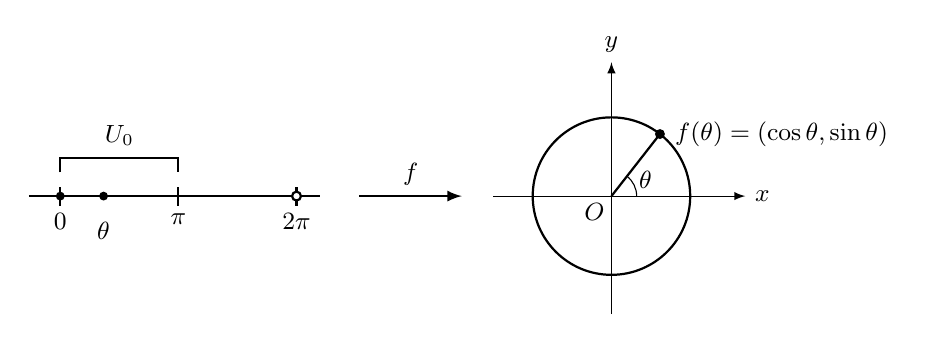
\begin{tikzpicture}[>=latex, scale=1.0]
    % 左: 实直线上的区间 [0, 2pi)
    \draw[thick] (-0.4, 0) -- (3.3, 0);
    \draw[thick] (0, -0.12) -- (0, 0.12) node[below=6pt] {\small $0$};
    \draw[thick] (1.5, -0.12) -- (1.5, 0.12) node[below=6pt] {\small $\pi$};
    \draw[thick] (3.0, -0.12) -- (3.0, 0.12) node[below=6pt] {\small $2\pi$};
    \fill (0, 0) circle (1.6pt);
    \draw[fill=white, thick] (3.0, 0) circle (1.6pt);
    \fill (0.55, 0) circle (1.6pt) node[below=6pt] {\small $\theta$};

    % U_0 的上方括号
    \draw[thick] (0, 0.3) -- (0, 0.48) -- (1.5, 0.48) -- (1.5, 0.3);
    \node[above=1pt] at (0.75, 0.48) {\small $U_{0}$};

    % 箭头 f
    \draw[->, thick] (3.8, 0) -- node[above] {\small $f$} (5.1, 0);

    % 右: 单位圆 S^1
    \begin{scope}[shift={(7.0, 0)}]
      \draw[->] (-1.5, 0) -- (1.7, 0) node[right] {\small $x$};
      \draw[->] (0, -1.5) -- (0, 1.7) node[above] {\small $y$};
      \node[below left=-1pt] at (0, 0) {\small $O$};

      \draw[thick] (0, 0) circle (1.0);

      \coordinate (P) at (52:1.0);
      \draw[thick] (0, 0) -- (P);
      \fill (P) circle (1.8pt);
      \node[right=2pt] at (P) {\small $f(\theta) = (\cos\theta, \sin\theta)$};
      \draw (0.32, 0) arc (0:52:0.32);
      \node at (26:0.48) {\small $\theta$};
    \end{scope}
  \end{tikzpicture}
  \caption{}\label{fig:7.3.2}
\end{figure}
\end{example}

\begin{example}\label{ex:7.3.5}
设 $X = Y = \{a, b\}$, $a \neq b$. 显然, 恒同映射
\[
  f = \operatorname{Id}_{X}\colon (X, \mathcal{T}_{\text{离散}}) \to (X, \mathcal{T}_{\text{平庸}})
\]
为一一连续映射, 但 $f^{-1}$ 不连续, 从而 $f$ 不为同胚. 事实上, 对 $f^{-1}(a) = a \in X$ 的开邻域 $\{a\}$, $a \in Y$ 的开邻域只有 $Y = \{a, b\}$, 显然 $f^{-1}(Y) = \{a, b\} \not\subset \{a\}$. 因此, $f^{-1}$ 在 $a$ 处不连续.
\end{example}

细心的读者会注意到\cref{ex:7.3.4}中 $X = [0, 2\pi)$ 非紧致, \cref{ex:7.3.5}中 $(Y, \mathcal{T}_{\text{平庸}})$ 不是 $T_{2}$ 空间, 它们都不符合\cref{thm:7.3.10}的条件.

我们知道, 连通、道路连通、紧致、可数紧致、序列紧致、列紧都为拓扑不变性, 作为它的应用, 我们往往可以判别两个拓扑空间不同胚.

\begin{example}\label{ex:7.3.6}
(1) $(\mathbb{Z}_{+}, \mathcal{T}_{1}) \not\cong (\mathbb{R}, \mathcal{T}_{2})$;

(2) $S^{n} \not\cong \mathbb{R}^{m}$, 其中 $S^{n}$ 为通常的 $n$ 维单位球面, $\mathbb{R}^{m}$ 为通常的 $m$ 维 Euclid 空间;

(3) $S^{1} \not\cong S^{2}$, 其中 $S^{1}$ 为通常的单位圆, $S^{2}$ 为通常的二维单位球面;

(4) $X \not\cong S^{1}$, 其中 $S^{1}$ 为通常的单位圆, $X = \{(x, y) \mid (x^{2} + y^{2})^{2} = a^{2}(x^{2} - y^{2})\} \subset \mathbb{R}^{2}$ ($a > 0$) 为平面上的双纽线.
\end{example}

\begin{proof}
(1) (反证) 假设 $(\mathbb{Z}_{+}, \mathcal{T}_{1}) \cong (\mathbb{R}, \mathcal{T}_{2})$, 则存在同胚 $f\colon \mathbb{Z}_{+} \to \mathbb{R}$. 因此, $\mathbb{Z}_{+}$ 与 $\mathbb{R}$ 在 $f$ 下一一对应, 但 $\mathbb{Z}_{+}$ 可数, $\mathbb{R}$ 不可数, 矛盾.

(2) (反证) 假设 $S^{n} \cong \mathbb{R}^{m}$, 则存在同胚 $f\colon S^{n} \to \mathbb{R}^{m}$. 由于 $S^{n}$ 紧致, 而 $\mathbb{R}^{m}$ 非紧致, 这与紧致为拓扑不变性相矛盾.

(3) (反证) 假设 $S^{1} \cong S^{2}$, 则存在同胚 $f\colon S^{1} \to S^{2}$. 于是, $f\colon S^{1} \setminus \{(1, 0), (-1, 0)\} \to S^{2} \setminus \{f(1, 0), f(-1, 0)\}$ 也为同胚. 由于 $S^{1} \setminus \{(1, 0), (-1, 0)\}$ 不连通, 而 $S^{2} \setminus \{f(1, 0), f(-1, 0)\}$ 连通 (\cref{ex:7.2.4}), 这与连通性为拓扑不变性相矛盾.

(4) (反证) 假设 $X \cong S^{1}$, 则存在同胚 $f\colon X \to S^{1}$. 于是, $f\colon X \setminus \{(0, 0)\} \to S^{1} \setminus \{f(0, 0)\}$ 也为同胚. 由于 $X \setminus \{(0, 0)\}$ 不连通, 而 $S^{1} \setminus \{f(0, 0)\}$ 连通, 这与连通为拓扑不变性相矛盾.
\end{proof}


\begin{exblock}{练习题 7.3}

  \item 证明: $A$ 为 $(X, \mathcal{T})$ 的紧致子集 $\iff (X, \mathcal{T})$ 的任一闭集类 $\mathcal{F}_{0} \subset \mathcal{F}$, 且 $A \cap \left(\bigcap\limits_{F \in \mathcal{F}_{0}} F\right) = \varnothing$, 则有 $A_{1}, A_{2}, \cdots, A_{k} \in \mathcal{F}_{0}$, 使得 $A \cap \left(\bigcap\limits_{i=1}^{k} A_{i}\right) = \varnothing$.

  \item 证明: $A$ 为 $(X, \mathcal{T})$ 的可数紧致子集 $\iff (X, \mathcal{F})$ 的任一可数闭集类 $\mathcal{F}_{0} \subset \mathcal{F}$, 且 $A \cap \left(\bigcap\limits_{F \in \mathcal{F}_{0}} F\right) = \varnothing$, 则有 $A_{1}, A_{2}, \cdots, A_{k} \in \mathcal{F}_{0}$, 使得 $A \cap \left(\bigcap\limits_{i=1}^{k} A_{i}\right) = \varnothing$.

  \item 设 $P_{i}\colon \mathbb{R}^{2} \to \mathbb{R}^{1}$, $P_{i}(x_{1}, x_{2}) = x_{i}$ 为投影算子, $A \subset \mathbb{R}^{2}$ 为 $(\mathbb{R}^{2}, \mathcal{T}_{\rho_{0}}^{2})$ 中的紧致集. 证明:
  \begin{enumerate}
    \item $P_{i}$ 为连续映射;
    \item $P_{i}(A)$ 也为 $(\mathbb{R}^{1}, \mathcal{T}_{\rho_{0}}^{1})$ 中的紧致集.
  \end{enumerate}

  \item 设 $A, B \subset \mathbb{R}^{1}$. 证明: $A \times B$ 为 $(\mathbb{R}^{2}, \mathcal{T}_{\rho_{0}}^{2})$ 中的紧致集 $\iff$ $A$ 与 $B$ 均为 $(\mathbb{R}^{1}, \mathcal{T}_{\rho_{0}}^{1})$ 中的紧致集.

  \item 证明: 拓扑空间 $(X, \mathcal{T})$ 的任何有限子集都为紧致子集.

  \item 设 $\mathcal{T}'$ 与 $\mathcal{T}$ 都为 $X$ 的拓扑, 且 $\mathcal{T}' \subset \mathcal{T}$. 证明: 当 $(X, \mathcal{T})$ 紧致时, $(X, \mathcal{T}')$ 也紧致.

  \item 证明: 拓扑空间 $(X, \mathcal{T})$ 中任何有限个紧致子集的并集仍是一个紧致子集.

  \item 证明: 拓扑空间 $(X, \mathcal{T})$ 中任何一族紧致闭子集的交仍是一个紧致闭集.
\end{exblock}

\begin{exblock}{思考题 7.3}

  \item 在\cref{thm:7.3.2}中, 证明: (3) $\Rightarrow$ (5), (5) $\Rightarrow$ (4).

  \item 设 $(X, \mathcal{T})$ 为 $T_{2}$ 空间, $A \subset X$ 为 $(X, \mathcal{T})$ 中的紧致子集, $x \in A^{c}$. 证明: $x$ 与 $A$ 分别存在开邻域 $U$ 与 $V$, 使得 $U \cap V = \varnothing$.

  \item 设 $(X, \mathcal{T})$ 为 $T_{2}$ 空间, 如果 $A$ 与 $B$ 为 $(X, \mathcal{T})$ 的不交紧致子集, 则 $A$ 与 $B$ 分别存在开邻域 $U$ 与 $V$, 使得 $U \cap V = \varnothing$.

  \item 证明: $T_{2}$ 空间 $(X, \mathcal{T})$ 中任意多个紧致子集的交仍为紧致子集.

  \item 设 $(X, \rho)$ 为度量空间, $A$ 为 $(X, \mathcal{T}_{\rho})$ 的列紧子集. 证明: $A$ 为有界闭集.

  \item (1) 设 $(X, \rho)$ 为度量空间. $X$ 中的两个非空子集 $A$ 与 $B$ 的距离 $\rho(A, B)$ 定义为
  \[
    \rho(A, B) = \inf\{\rho(x, y) \mid x \in A, y \in B\}.
  \]
  当 $A = \{a\}$ 时, $\rho(a, B) = \rho(\{a\}, B) = \inf\{\rho(a, y) \mid y \in B\}$ 称为 $a$ 与集合 $B$ 之间的距离.

  证明:
  \begin{enumerate}
    \item 如果 $A$ 与 $B$ 为 $(X, \rho)$ 中的两个非空紧致子集, 则 $\exists a \in A$ 与 $b \in B$, s.t. $\rho(a, b) = \rho(A, B)$;

    \item 设 $X = \{-1\} \cup (0, 1)$ 作为 $(\mathbb{R}^{1}, \mathcal{T}_{\rho_{0}}^{1})$ 的子度量空间, $A = \{-1\}$ 与 $B = (0, 1)$ 分别为 $X$ 的紧致子集与闭集, 易见, 它无 (1) 中的结论;

    \item 设 $A$ 与 $B$ 分别为 $(\mathbb{R}^{n}, \rho_{0}^{n})$ 中的非空紧致子集与非空闭集, 则 $\exists a \in A$ 与 $b \in B$, s.t. $\rho_{0}^{n}(a, b) = \rho_{0}^{n}(A, B)$;

    \item 在 $(\mathbb{R}^{2}, \rho_{0}^{2})$ 中给出两个不相交的非空闲集 $A$ 与 $B$, 使得 $\rho_{0}^{2}(A, B) = 0$, 但不存在 $a \in A$, 不存在 $b \in B$, s.t. $\rho_{0}^{2}(a, b) = \rho_{0}^{2}(A, B)$;

    \item 设 $A$ 与 $B$ 分别为度量空间 $(X, \rho)$ 的非空紧子集与非空闭集. 证明:
    \[
      \rho(A, B) = 0 \iff A \cap B \neq \varnothing.
    \]
  \end{enumerate}

  \item 证明: 不存在由 $[0, 1]$ 到圆周上的一一连续映射.

  \item 证明: 不存在由 $[0, 1]$ 到 $[0, 1] \times [0, 1]$ 上的一一连续映射.

  \item 设 $E \subset \mathbb{R}^{n}$, $f\colon E \to \mathbb{R}^{m}$.
  \begin{enumerate}
    \item 如果 $E$ 为闭集, $f$ 连续, 则 $f$ 的图像
    \[
      G(f) = \{(x, f(x)) \mid x \in E\}
    \]
    为 $\mathbb{R}^{n+m}$ 中的闭集;

    \item 如果 $E$ 为紧致集, $f$ 连续, 则 $G(f)$ 也为紧致集;

    \item 如果 $G(f)$ 为紧致集, 则 $f$ 连续;

    \item 如果 $G(f)$ 为闭集, $f$ 是否连续?
  \end{enumerate}
\end{exblock}
% ==================================================================
%  §7.4  零值定理、介值定理、最值定理及一致连续性定理
%  源：徐森林、薛春华《数学分析》第二册，印刷页 35-40 (PDF p. 41-46)
%  底本：PaddleOCR-VL-1.6 JSON/MD 识别结果，人工逐字核校与公式精修
%  规范：全西文标点，忠实原文定理、定义、引理、例题、练习题编号与推导
% ==================================================================

\section{零值定理、介值定理、最值定理及一致连续性定理}\label{sec:7.4}

在这一节, 我们将有界闭区间 $[a, b]$ 上连续函数的零值定理, 介值定理, 最值定理及一致连续性定理推广到 $n$ 维 Euclid 空间, 以至拓扑空间.

\begin{theorem}[介值定理]\label{thm:7.4.1}
设 $(X, \mathcal{T})$ 连通, $(\mathbb{R}^{1}, \mathcal{T}_{\rho_{0}}^{1}) = (\mathbb{R}, \mathcal{T}_{\rho_{0}}^{1})$ 为通常的实直线, $f\colon X \to \mathbb{R}^{1}$ 为连续函数, $p, q \in X$, 则 $f$ 达到介于 $f(p)$ 与 $f(q)$ 之间的一切值, 即 $\exists \xi \in X$, s. t.
\[
  f(\xi) = r \in [\min\{f(p), f(q)\}, \max\{f(p), f(q)\}].
\]
\end{theorem}

\begin{proof}
由\cref{thm:7.2.7}(1), $f(X)$ 为 $(\mathbb{R}^{1}, \mathcal{T}_{\rho_{0}}^{1})$ 中的连通集, 即为实直线上的区间 (当 $f$ 为常值函数时缩成一点), 所以 $f$ 达到 $f(p)$ 与 $f(q)$ 之间的一切值.
\end{proof}

\begin{theorem}[零 (根) 值定理]\label{thm:7.4.2}
设 $(X, \mathcal{T})$ 连通, $f\colon X \to \mathbb{R}$ 为连续函数, $p, q \in X$, 如果 $f(p)f(q) \leqslant 0$, 则 $\exists \xi \in X$, s. t. $f(\xi) = 0$.
\end{theorem}

\begin{proof}
因为 $f(p)f(q) \leqslant 0$, 所以 $r = 0 \in [\min\{f(p), f(q)\}, \max\{f(p), f(q)\}]$, 由\cref{thm:7.4.1} (介值定理), $\exists \xi \in X$, s. t. $f(\xi) = 0$.
\end{proof}

\begin{example}[Borsuk-Ulam 定理]\label{ex:7.4.1}
设 $S^{n} = \left\{(x_{1}, x_{2}, \cdots, x_{n+1}) \mid \sum\limits_{i=1}^{n+1} x_{i}^{2} = 1\right\} \subset \mathbb{R}^{n+1}$ 为 $n$ 维单位球面 ($n \in \mathbb{Z}_{+}$), $f\colon S^{n} \to \mathbb{R}^{1}$ 为连续函数. 则 $\exists \xi \in S^{n}$, s. t. $f(\xi) = f(-\xi)$.
\end{example}

\begin{proof}
$\forall p, q \in S^{n}$, 取一个过球心的二维平面, s. t. $e_{1} = p$, $\{e_{1}, e_{2}\}$ 构成该平面的规范正交基, 而 $q$ 也在此平面内 (\cref{fig:7.4.1}). 于是, $q = \cos\theta_{0} e_{1} + \sin\theta_{0} e_{2}$.

显然, $\boldsymbol{\sigma}(t) = \cos t\theta_{0} e_{1} + \sin t\theta_{0} e_{2}$ 为球面 $S^{n}$ 上连接 $p$ 与 $q$ 的一条道路. 因此, $S^{n}$ 是道路连通的, 根据\cref{thm:7.2.5}, $S^{n}$ 是连通的.

\begin{figure}[htbp]
  \centering
  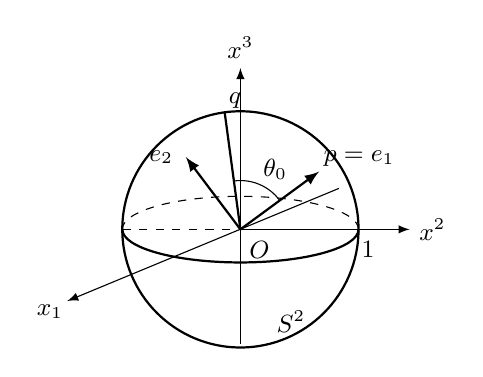
\begin{tikzpicture}[>=latex, scale=1.0]
    % ---- 球面 S^2 ----
    \draw[thick] (0, 0) circle (1.5);
    % 赤道椭圆: 后半虚线、前半实线; 以及过球心的虚线直径
    \draw[dashed] (1.5, 0) arc (0:180:1.5 and 0.42);
    \draw[thick] (1.5, 0) arc (0:-180:1.5 and 0.42);
    \draw[dashed] (-1.5, 0) -- (1.5, 0);
    % ---- 坐标轴 ----
    \draw[->] (0, -1.45) -- (0, 2.05) node[above] {\small $x^{3}$};
    \draw[->] (0, 0) -- (2.15, 0) node[right] {\small $x^{2}$};
    \draw[->] (1.25, 0.52) -- (-2.20, -0.91) node[below left=-2pt] {\small $x_{1}$};
    \node[below=1pt] at (1.62, 0) {\small $1$};
    \node[below right=-2pt] at (0.06, -0.10) {\small $O$};
    % ---- 球面上的点 q, 向径 Oq ----
    \coordinate (q) at (-0.20, 1.487);
    \draw[thick] (0, 0) -- (q);
    \node[above right=-2pt] at (q) {\small $\boldsymbol{q}$};
    % ---- 向量 p = e_1 与 e_2 ----
    \draw[->, thick] (0, 0) -- (36.3:1.24) node[above right=-2pt] {\small $\boldsymbol{p} = \boldsymbol{e}_{1}$};
    \draw[->, thick] (0, 0) -- (127:1.15) node[left=1pt] {\small $\boldsymbol{e}_{2}$};
    % ---- 夹角 theta_0 ----
    \draw (36.3:0.62) arc (36.3:97.7:0.62);
    \node at (60:0.88) {\small $\theta_{0}$};
    % ---- 球面标签 ----
    \node at (0.64, -1.17) {\small $S^{2}$};
  \end{tikzpicture}
  \caption{}\label{fig:7.4.1}
\end{figure}

令
\[
  F(\boldsymbol{x}) = f(\boldsymbol{x}) - f(-\boldsymbol{x}),\quad \boldsymbol{x} = (x_{1}, x_{2}, x_{3}),
\]
则
\[
  \begin{aligned}
    F(\boldsymbol{p})F(-\boldsymbol{p}) &= [f(\boldsymbol{p}) - f(-\boldsymbol{p})][f(-\boldsymbol{p}) - f(\boldsymbol{p})]\\
    &= -[f(\boldsymbol{p}) - f(-\boldsymbol{p})]^{2} \leqslant 0.
  \end{aligned}
\]
根据\cref{thm:7.4.2}, $\exists \xi \in S^{n}$, s. t.
\[
  0 = F(\xi) = f(\xi) - f(-\xi),
\]
即 $f(\xi) = f(-\xi)$.
\end{proof}

\begin{theorem}[最值定理]\label{thm:7.4.3}
设 $(X, \mathcal{T})$ 为紧致 (或可数紧致, 或序列紧致) 空间, $(\mathbb{R}^{1}, \mathcal{T}_{\rho_{0}}^{1})$ 为通常的一维 Euclid 空间, $f\colon X \to \mathbb{R}^{1}$ 为连续函数, 则 $f$ 在 $X$ 上必达到最大值与最小值. 此时, $f(X) = [m, M]$, 其中 $m = \min\limits_{x \in X} f(x)$, $M = \max\limits_{x \in X} f(x)$.
\end{theorem}

\begin{proof}
由\cref{thm:7.3.7}, $f(X)$ 为 $(\mathbb{R}^{1}, \mathcal{T}_{\rho_{0}}^{1})$ 中的紧致 (或可数紧致, 或序列紧致) 子集. 再由\cref{thm:7.3.6}知, $f(X)$ 为 $(\mathbb{R}^{1}, \mathcal{T}_{\rho_{0}}^{1})$ 中的有界闭集. 因此 $\min\limits_{x \in X} f(x)$, $\max\limits_{x \in X} f(x)$ 分别为 $f$ 在 $X$ 上的最小值与最大值.
\end{proof}

\begin{corollary}\label{cor:7.4.1}
设 $(X, \mathcal{T}_{\rho})$ 为列紧度量空间, $(\mathbb{R}^{1}, \mathcal{T}_{\rho_{0}}^{1})$ 为通常的一维 Euclid 空间, $f\colon X \to \mathbb{R}^{1}$ 为连续函数, 则 $f$ 在 $X$ 上必达到最大值与最小值.
\end{corollary}

\begin{proof}
由\cref{thm:7.3.2}, 列紧度量空间 $(X, \mathcal{T}_{\rho})$ 也是可数紧致, 也是序列紧致的, 再根据\cref{thm:7.4.3}, $f$ 在 $X$ 上必达到最大值与最小值.
\end{proof}

\begin{theorem}[Lebesgue 数定理]\label{thm:7.4.4}
设 $(X, \rho)$ 为序列紧致 (或可数紧致, 或列紧, 或紧致) 度量空间, $\mathcal{T}$ 为 $X$ 的一个开覆盖 (即 $X = \bigcup\limits_{I \in \mathcal{T}} I$, $I$ 为 $(X, \mathcal{T}_{\rho})$ 中的开集), 则存在一个正数 $\lambda = \lambda(\mathcal{T})$ 具有性质: 如果 $A \subset X$, 其直径
\[
  d(A) = \operatorname{diam} A = \sup\{\rho(x', x'') \mid x', x'' \in A\} < \lambda = \lambda(\mathcal{T})
\]
时, 必有 $I \in \mathcal{T}$, s. t. $A \subset I$. 我们称 $\lambda = \lambda(\mathcal{T})$ 为开覆盖 $\mathcal{T}$ 的一个 Lebesgue 数.
\end{theorem}

\begin{proof}
完全仿照\extref{定理 2.5.6} 的证明.

(反证) 假设结论不成立, 则 $\forall n \in \mathbb{Z}_{+}$, $\exists A_{n} \subset X$, 它的直径 $d(A_{n}) < \dfrac{1}{n}$, 而不存在 $I \in \mathcal{T}$, s. t. $A_{n} \subset I$. 在每个 $A_{n}$ 中取 $a_{n}$. 根据 $(X, \rho)$ 为序列紧致空间, 存在子列 $\{a_{n_{k}}\}$ 收敛于 $a_{0} \in X$. 因为 $\mathcal{T}$ 为 $(X, \mathcal{T}_{\rho})$ 的一个开覆盖, 故存在 $I_{0} \in \mathcal{T}$, 使得 $a_{0} \in I_{0}$. 因为 $I_{0}$ 为开集, 当 $X \setminus I_{0} \neq \varnothing$ 时, 点 $a_{0}$ 到集合 $X \setminus I_{0}$ 的距离
\[
  d = \rho(a_{0}, X \setminus I_{0}) = \inf\{\rho(a_{0}, x) \mid x \in X \setminus I_{0}\} > 0,
\]
由于 $\lim\limits_{k \to +\infty} a_{n_{k}} = a_{0}$, 所以, $\exists n_{k_{0}}$, s. t. $n_{k_{0}} < \dfrac{2}{d}$ 与 $\rho(a_{0}, a_{n_{k_{0}}}) < \dfrac{d}{2}$. 于是, $\forall x \in A_{n_{k_{0}}}$, 有
\[
  \rho(a_{0}, x) \leqslant \rho(a_{0}, a_{n_{k_{0}}}) + \rho(a_{n_{k_{0}}}, x) < \frac{d}{2} + \frac{1}{n_{k_{0}}} < \frac{d}{2} + \frac{d}{2} = d,
\]
因而, $A_{n_{k_{0}}} \subset I_{0} \in \mathcal{T}$; 当 $X \setminus I_{0} = \varnothing$ 时, $A_{n} \subset X \subset I_{0}$. 这与不存在 $I \in \mathcal{T}$, s. t. $A_{n_{k_{0}}} \subset I$ 相矛盾.
\end{proof}

\begin{theorem}[一致连续性定理]\label{thm:7.4.5}
设 $(X, \rho_{1})$ 为序列紧致 (或可数紧致, 或列紧, 或紧致) 的度量空间, $(Y, \rho_{2})$ 为度量空间, $f\colon X \to Y$ 为连续映射, 则 $f$ 在 $X$ 上一致连续, 即 $\forall \varepsilon > 0$, $\exists \delta > 0$, 当 $x', x'' \in X$, $\rho_{1}(x', x'') < \delta$ 时, 有 $\rho_{2}(f(x'), f(x'')) < \varepsilon$.
\end{theorem}

\begin{proof}[证法 1]
根据\cref{thm:7.3.2}, 只需考虑序列紧致情况.

(反证) 假设 $f$ 在 $X$ 上不一致连续, 则 $\exists \varepsilon_{0} > 0$, $\forall n \in \mathbb{Z}_{+}$, 必有 $x_{n}', x_{n}''$, s. t. $\rho_{1}(x_{n}', x_{n}'') < \dfrac{1}{n}$, 但 $\rho_{2}(f(x_{n}'), f(x_{n}'')) \geqslant \varepsilon_{0}$. 因为 $(X, \mathcal{T}_{\rho_{1}})$ 序列紧致, 故 $\{x_{n}'\}$ 必有收敛子列 $\{x_{n_{k}}'\}$, 记 $\lim\limits_{k \to +\infty} x_{n_{k}}' = x_{0} \in X$. 由于 $\rho_{1}(x_{n}', x_{n}'') < \dfrac{1}{n}$, 故
\[
  0 \leqslant \rho_{1}(x_{n_{k}}'', x_{0}) \leqslant \rho_{1}(x_{n_{k}}'', x_{n_{k}}') + \rho_{1}(x_{n_{k}}', x_{0}) < \frac{1}{n_{k}} + \rho_{1}(x_{n_{k}}', x_{0}) \to 0\ (k \to +\infty),
\]
即
\[
  \lim\limits_{k \to +\infty} \rho_{1}(x_{n_{k}}'', x_{0}) = 0,\quad \lim\limits_{k \to +\infty} x_{n_{k}}'' = x_{0}.
\]
于是, 由 $f$ 为 $X$ 上的连续函数, $\exists K \in \mathbb{Z}_{+}$, 当 $k > K$ 时, 有
\[
  \begin{aligned}
    \varepsilon_{0} &\leqslant \rho_{2}\left(f(\boldsymbol{x}_{n_{k}}'), f(\boldsymbol{x}_{n_{k}}'')\right)\\
    &\leqslant \rho_{2}\left(f(\boldsymbol{x}_{n_{k}}'), f(\boldsymbol{x}_{0})\right) + \rho_{2}\left(f(\boldsymbol{x}_{0}), f(\boldsymbol{x}_{n_{k}}'')\right)\\
    &< \frac{\varepsilon_{0}}{2} + \frac{\varepsilon_{0}}{2} = \varepsilon_{0},
  \end{aligned}
\]
矛盾. 所以, $f$ 在 $X$ 上一致连续. \noqedhere
\end{proof}

\begin{proof}[证法 2]
设 $(X, \mathcal{T}_{\rho_{1}})$ 紧致. $\forall \varepsilon > 0$, 因为 $f$ 在 $X$ 上连续, 故对 $x \in X$, $\exists \delta(x) > 0$, s. t. 当 $x' \in X$, 且 $\rho_{1}(x', x) < \delta(x)$ 时, 有 $\rho_{2}(f(x'), f(x)) < \dfrac{\varepsilon}{2}$.

显然, 开球族 $\mathcal{T} = \left\{B\left(x; \dfrac{\delta(x)}{2}\right) \middle| x \in X\right\}$ 为紧致空间 $(X, \mathcal{T}_{\rho_{1}})$ 的一个开覆盖. 因此, 存在有限子覆盖 $\mathcal{T}_{1} = \left\{B\left(x_{i}; \dfrac{\delta(x_{i})}{2}\right) \middle| i = 1, 2, \cdots, m\right\}$. 令
\[
  \delta = \min\left\{\frac{\delta(x_{i})}{2} \bigg| i = 1, 2, \cdots, m\right\},
\]
则 $\forall x', x'' \in X$, 当 $\rho_{1}(x', x'') < \delta$ 时, 如果 $x' \in B\left(x_{i_{0}}; \dfrac{\delta(x_{i_{0}})}{2}\right)$, 必有 $x', x'' \in B(x_{i_{0}}; \delta(x_{i_{0}}))$, 从而
\[
  \rho_{2}\left(f(x'), f(x'')\right) \leqslant \rho_{2}\left(f(x'), f(x_{i_{0}})\right) + \rho_{2}\left(f(x_{i_{0}}), f(x'')\right) < \frac{\varepsilon}{2} + \frac{\varepsilon}{2} = \varepsilon,
\]
即 $f$ 在 $X$ 上是一致连续的. \noqedhere
\end{proof}

\begin{proof}[证法 3]
设 $(X, \mathcal{T}_{\rho})$ 序列紧致. 在证法 2 中, 由于 $\mathcal{T}_{1} = \{B(x; \delta(x)) \mid x \in X\}$ 为序列紧致集 $X$ 的一个开覆盖. 根据\cref{thm:7.4.4}, 存在 Lebesgue 数 $\lambda(\mathcal{T}_{1}) > 0$. 对于 $\varepsilon > 0$, 取 $\delta = \lambda(\mathcal{T}_{1})$, 则当 $x', x'' \in X$, 且 $\operatorname{diam}\{x', x''\} = \rho(x', x'') < \delta = \lambda(\mathcal{T}_{1})$ 时, 存在 $B(x_{0}; \delta(x_{0})) \in \mathcal{T}_{1}$, 使得 $\{x', x''\} \subseteq B(x_{0}; \delta(x_{0}))$, 从而,
\[
  \rho_{2}\left(f(x'), f(x'')\right) \leqslant \rho_{2}\left(f(x'), f(x_{0})\right) + \rho_{2}\left(f(x_{0}), f(x'')\right) < \frac{\varepsilon}{2} + \frac{\varepsilon}{2} = \varepsilon.
\]
这就证明了 $f$ 在 $X$ 上是一致连续的.
\end{proof}

\begin{theorem}[延拓定理]\label{thm:7.4.6}
设 $(X, \rho_{1})$ 与 $(Y, \rho_{2})$ 为度量空间, $A \subset X$.
\begin{enumerate}
  \item 如果 $\overline{A}$ 为 $(X, \mathcal{T}_{\rho_{1}})$ 的序列紧致 (或可数紧致, 或列紧, 或紧致) 子集, $f\colon \overline{A} \to Y$ 连续, 则 $f$ 在 $\overline{A}$ (当然也在 $A$) 上一致连续.

  \item 如果 $f\colon A \to Y$ 一致连续, $\overline{f(A)}$ 为 $(Y, \rho_{2})$ 的完备子度量空间, 则存在连续映射 $\tilde{f}\colon \overline{A} \to Y$, 使得 $\tilde{f}|A = f|A$, 即 $\tilde{f}$ 为 $f$ 的 (连续) 延拓.
\end{enumerate}
\end{theorem}

\begin{proof}
(1) 由\cref{thm:7.4.5}推得.

(2) $\forall x_{0} \in \overline{A}$, $x_{n} \in A$, $x_{n} \to x_{0}\ (n \to +\infty)$, 必有 $\lim\limits_{n \to +\infty} f(x_{n})$ 存在, 且 $\lim\limits_{n \to +\infty} f(x_{n}) \in \overline{f(A)}$. 事实上, $\forall \varepsilon > 0$, 由于 $f$ 在 $A$ 上一致连续, 所以存在 $\delta > 0$, 当 $\rho_{1}(x', x'') < \delta$ 时, 有 $\rho_{2}(f(x'), f(x'')) < \varepsilon$. 于是, $\exists N \in \mathbb{Z}_{+}$, 当 $n, m > N$ 时, $\rho_{1}(x_{n}, x_{m}) < \delta$, 从而 $\rho_{2}(f(x_{n}), f(x_{m})) < \varepsilon$. 这意味着 $\{f(x_{n})\}$ 为 $\overline{f(A)} \subset Y$ 中的 Cauchy (基本) 点列. 因为 $\overline{f(A)}$ 为 $(Y, \rho_{2})$ 的完备子度量空间, 所以 $\{f(x_{n})\}$ 在 $\overline{f(A)}$ 中必收敛, 即 $\lim\limits_{n \to +\infty} f(x_{n})$ 存在且属于 $\overline{f(A)}$. 再证 $\lim\limits_{n \to +\infty} f(x_{n})$ 与点列 $\{x_{n}\}$, $x_{n} \to x_{0}\ (n \to +\infty)$ 的选取无关. 如果 $y_{n} \in A$, $y_{n} \to x_{0}\ (n \to +\infty)$, 则 $\{z_{n}\} = \{x_{1}, y_{1}, x_{2}, y_{2}, \cdots, x_{n}, y_{n}, \cdots\}$ 也收敛于 $x_{0}$, 所以 $\{f(z_{n})\}$ 也收敛, 且
\[
  \lim_{n \to +\infty} f(x_{n}) = \lim_{n \to +\infty} f(z_{n}) = \lim_{n \to +\infty} f(y_{n}).
\]
由此与归结原则可知, $\lim\limits_{\substack{x \to x_{0} \\ x \in A}} f(x)$ 存在且属于 $\overline{f(A)}$. 我们定义
\[
  \tilde{f}(x_{0}) = \lim_{\substack{x \to x_{0} \\ x \in A}} f(x).
\]
易见, $\tilde{f}$ 为 $\overline{A}$ 上的连续映射, 且 $\tilde{f}|A = f|A$, 即 $\tilde{f}$ 为 $f$ 的 (连续) 延拓.
\end{proof}

作为一致连续的应用, 我们来考虑下面的重要例子.

\begin{example}\label{ex:7.4.2}
设 $X = ([0, 1] \times \{0\}) \cup \left(\left\{0, 1, \dfrac{1}{2}, \cdots, \dfrac{1}{n}, \cdots\right\} \times [0, 1]\right) \subset \mathbb{R}^{2}$, 称它为篦式空间. 则:

(1) 点 $(0, 1)$ 为 $X$ 的形变收缩核, 即存在连续映射 $F\colon X \times [0, 1] \to X$, 使得
\[
  F((x_{1}, x_{2}), 0) = (x_{1}, x_{2}) = \operatorname{Id}_{X}(x_{1}, x_{2}),
\]
\[
  F((x_{1}, x_{2}), 1) = (0, 1) = C_{(0, 1)}(x_{1}, x_{2}),
\]
其中 $\operatorname{Id}_{X}\colon X \to X$ 为 $X$ 上的恒同映射, $C_{(0, 1)}$ 为 $X$ 上的常值映射.

(2) 点 $(0, 1)$ 不为 $X$ 上的强形变收缩核, 即不存在连续映射 $G\colon X \times [0, 1] \to X$
\[
  G((x_{1}, x_{2}), 0) = (x_{1}, x_{2}) = \operatorname{Id}_{X}(x_{1}, x_{2}),
\]
\[
  G((x_{1}, x_{2}), 1) = (0, 1) = C_{(0, 1)}(x_{1}, x_{2}),
\]
\[
  G((0, 1), t) = (0, 1),\quad \forall t \in [0, 1].
\]

(3) 点 $(0, 0)$ 为 $X$ 上的强形变收缩核 (读者自证).
\end{example}

\begin{proof}
(1) 令 $F\colon X \times [0, 1] \to X$,
\[
  F((x_{1}, x_{2}), t) = \begin{cases}
    (x_{1}, (1 - 3t)x_{2}), & 0 \leqslant t \leqslant \dfrac{1}{3},\\[6pt]
    ((2 - 3t)x_{1}, 0), & \dfrac{1}{3} < t \leqslant \dfrac{2}{3},\\[6pt]
    (0, 3t - 2), & \dfrac{2}{3} < t \leqslant 1
  \end{cases}
\]
为所需的形变收缩, 因此, $(0, 1)$ 为 $X$ 的形变收缩核.

(2) (反证) 假设 $(0, 1)$ 为 $X$ 的强形变收缩核, 即存在 (2) 中所述的连续映射 $G\colon X \times [0, 1] \to X$. 因为 $X \times [0, 1]$ 为紧致集, 故必一致连续. 从而对 $\varepsilon_{0} = \dfrac{1}{2}$, $\exists \delta > 0$, 当
\[
  \left\|(x_{1}, x_{2}, t) - (x_{1}', x_{2}', t')\right\| < \delta
\]
时, 有
\[
  \left\|G(x_{1}, x_{2}, t) - G(x_{1}', x_{2}', t')\right\| < \varepsilon_{0} = \frac{1}{2}.
\]
因此, 当 $\left\|(0, 1, t) - \left(\dfrac{1}{n}, 1, t\right)\right\| = \left\|\left(\dfrac{1}{n}, 0, 0\right)\right\| = \dfrac{1}{n} < \delta$ 时,
\[
  \begin{aligned}
    \left\|(0, 1) - G\left(\frac{1}{n}, 1, t\right)\right\| &= \left\|G(0, 1, t) - G\left(\frac{1}{n}, 1, t\right)\right\|\\
    &< \varepsilon_{0} = \frac{1}{2}.
  \end{aligned}
\]
由此得 $G\left(\dfrac{1}{n}, 1, t\right) \in B\left((0, 1); \dfrac{1}{2}\right)$, $\forall t \in [0, 1]$.

于是, $G\left(\dfrac{1}{n}, 1, t\right)$ 为开球 $B\left((0, 1); \dfrac{1}{2}\right)$ 中连接 $G\left(\left(\dfrac{1}{n}, 1\right), 1\right) = (0, 1)$ 与 $G\left(\left(\dfrac{1}{n}, 1\right), 0\right) = \left(\dfrac{1}{n}, 1\right)$ 的一条道路, 这与\cref{fig:7.4.2}中明显地在 $B\left((0, 1); \dfrac{1}{2}\right)$ 中无一条道路连接 $\left(\dfrac{1}{n}, 1\right)$ 与 $(0, 1)$ 相矛盾.
\end{proof}

\begin{figure}[htbp]
  \centering
  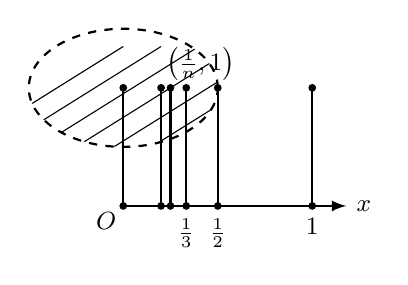
\begin{tikzpicture}[>=latex, x=2.4cm, y=1.5cm]
    % ---- 篦齿: x = 0, 1/5, 1/4, 1/3, 1/2, 1 ----
    \foreach \x in {0, 0.2, 0.25, 0.3333, 0.5, 1}{
      \draw[thick] (\x, 0) -- (\x, 1);
      \fill (\x, 1) circle (1.4pt);
      \fill (\x, 0) circle (1.4pt);
    }
    % ---- x 轴 ----
    \draw[->, thick] (0, 0) -- (1.18, 0) node[right] {\small $x$};
    \node[below left=-1pt] at (0, 0) {\small $O$};
    \node[below=1pt] at (0.3333, 0) {\small $\frac{1}{3}$};
    \node[below=1pt] at (0.5, 0) {\small $\frac{1}{2}$};
    \node[below=1pt] at (1, 0) {\small $1$};
    % ---- 开球 B((0,1); 1/2): 虚线圆 + 斜线阴影 ----
    \begin{scope}
      \clip (0, 1) circle (0.5);
      \foreach \k in {-1.0, -0.8, ..., 0.8}{
        \draw[thin] (\k, 0.35) -- (\k + 1.0, 1.35);
      }
    \end{scope}
    \draw[dashed, thick] (0, 1) circle (0.5);
    \node[right=1pt] at (0.16, 1.20) {\small $\left(\frac{1}{n}, 1\right)$};
  \end{tikzpicture}
  \caption{}\label{fig:7.4.2}
\end{figure}

\begin{exblock}{练习题 7.4}
  \item 设 $(X, \rho_{1})$ 与 $(Y, \rho_{2})$ 均为度量空间, $f\colon X \to Y$ 为一致连续映射, 证明: $f$ 为连续映射.

  \item 设 $(X, \rho_{1})$ 与 $(Y, \rho_{2})$ 均为度量空间, $f\colon X \to Y$ 为映射, 如果 $\exists \alpha \in (0, 1)$, s. t.
  \[
    \rho_{2}(f(x'), f(x'')) \leqslant \alpha \rho_{1}(x', x''),\quad \forall x', x'' \in X,
  \]
  则称 $f$ 为一个压缩映射. 显然, 它满足 Lipschitz 条件, 也为一致连续映射, 当然是连续映射. 当 $(X, \rho)$ 为完备度量空间, $f\colon X \to X$ 为压缩映射时, 令 $x_{n+1} = f(x_{n})$, 证明:
  \begin{enumerate}
    \item $\{x_{n}\}$ 为 $(X, \rho)$ 中的 Cauchy (基本) 点列, 记 $x_{0} = \lim\limits_{n \to +\infty} x_{n}$. 则 $f(x_{0}) = x_{0}$, 即 $x_{0}$ 为 $f$ 的一个不动点;
    \item $f$ 有惟一的一个不动点, 即 $\exists_{1}\xi \in X$, s. t. $f(\xi) = \xi$.
  \end{enumerate}

  \item 设 $A \subset \mathbb{R}^{n}$ 为非空集合, 证明: 点 $x$ 到 $A$ 的距离
  \[
    f_{A}(x) = \rho(x, A) = \inf_{y \in A} \rho(x, y)
  \]
  为 $\mathbb{R}^{n}$ 上的一致连续函数.
\end{exblock}

\begin{exblock}{思考题 7.4}
  \item 设 $\varphi\colon S^{n} \to S^{n}$ 为一个同胚, 满足: $\forall x \in S^{n}$, 有 $\varphi(\varphi(x)) = x$, 其中 $n \in \mathbb{Z}_{+}$. 证明: 对任何连续映射 $f\colon S^{n} \to \mathbb{R}$, $\exists \xi \in S^{n}$, s. t. $f(\xi) = f(\varphi(\xi))$. 当 $\varphi(x) = -x$ 时, 它就是\cref{ex:7.4.1}.

  \item 设 $(\mathbb{R}^{n}, \mathcal{T}_{\rho_{0}^{n}})$ 为 $n$ 维 Euclid 空间, $f\colon \mathbb{R}^{n} \to \mathbb{R}^{1}$ 为连续映射. 证明: 在 $\mathbb{R}^{1}$ 中最多存在两个点, 它在 $f$ 下的原像为非空的至多可数集.

  \item 设 $\boldsymbol{A} = (a_{ij})$ 为 $n \times n$ 的实方阵, 将它视为 $\mathbb{R}^{n^{2}}$ 中一个点 $(a_{11}, a_{12}, \cdots,\allowbreak a_{1n}, a_{21}, a_{22}, \cdots,\allowbreak a_{2n}, \cdots,\allowbreak a_{n1}, a_{n2}, \cdots, a_{nn})$. 于是, 将 $\{A = (a_{ij}) \mid a_{ij} \in \mathbb{R}\}$ 视为 $n^{2}$ 维 Euclid 空间 $(\mathbb{R}^{n^{2}}, \mathcal{T}_{\rho_{0}}^{n^{2}})$. 考虑 $n$ 阶正交群
  \[
    \boldsymbol{O}(n) = \boldsymbol{O}(n, \mathbb{R}) = \{\boldsymbol{P} \mid \boldsymbol{P}\boldsymbol{P}' = \boldsymbol{P}'\boldsymbol{P} = \boldsymbol{I},\ \boldsymbol{P} \text{ 为 } n \times n \text{ 实矩阵}\},
  \]
  其中 $\boldsymbol{I}$ 为单位矩阵, $P$ 为 $n \times n$ 实矩阵. 满足 $PP' = P'P = I$ 的实矩阵 $P$ 称为 $n$ 阶 (实) 正交矩阵. 显然, 有 $(\det P)^{2} = \det P \det P' = \det PP' = \det I = 1$, $\det P = \pm 1$. 证明:
  \begin{enumerate}
    \item $O(n)$ 为 $\mathbb{R}^{n^{2}}$ 中的有界闭集, 即为紧致集;
    \item $O^{+}(n) = O^{+}(n, \mathbb{R}) = \{P \mid PP' = P'P = I, \det P = 1\}$ 与 $O^{-}(n) = O^{-}(n, \mathbb{R}) = \{P \mid PP' = P'P = I, \det P = -1\}$ 都是道路连通的;
    \item $O(n)$ 不是道路连通的.
  \end{enumerate}

  \item 设 $\mathrm{GL}(n, \mathbb{R}) = \{A = (a_{ij}) \mid \det A \neq 0,\ A \text{ 为 } n \times n \text{ 实矩阵}\}$, 称它为 $n$ 阶一般线性群. 证明:
  \begin{enumerate}
    \item $\mathrm{GL}(n, \mathbb{R})$ 非紧致;
    \item $\mathrm{GL}^{+}(n, \mathbb{R}) = \{A \mid \det A > 0,\ A \text{ 为 } n \times n \text{ 实矩阵}\}$ 与 $\mathrm{GL}^{-}(n, \mathbb{R}) = \{A \mid \det A < 0,\ A \text{ 为 } n \times n \text{ 实矩阵}\}$ 都是道路连通的;
    \item $\mathrm{GL}(n; \mathbb{R})$ 不是道路连通的.
  \end{enumerate}
\end{exblock}

% ==================================================================
%  §7.5  n 元函数的连续与极限
%  源：徐森林、薛春华《数学分析》第二册，印刷页 40-51 (PDF p. 46-57)
%  底本：PaddleOCR-VL-1.6 JSON/MD 识别结果，人工逐字核校与公式精修
%  规范：全西文标点，忠实原文定义、注、定理、例题、练习题编号与推导
% ==================================================================

\section{$n$ 元函数的连续与极限}\label{sec:7.5}

设 $A \subset \mathbb{R}^{n}$, $f\colon A \to \mathbb{R}^{1}$ 为 $n$ 元函数,
\[
  x = (x_{1}, x_{2}, \cdots, x_{n}) \mapsto y = f(x) = f(x_{1}, x_{2}, \cdots, x_{n}) \in \mathbb{R}^{1}.
\]

\begin{definition}\label{def:7.5.1}
设 $A \subset \mathbb{R}^{n}$, $x^{0} \in \overline{A}$. 如果 $\forall \varepsilon > 0$, $\exists \delta > 0$, 当 $x \in A$, 且 $0 < \|x - x^{0}\| < \delta$ 时, 有
\[
  |f(x) - l| < \varepsilon,
\]
则称 $f$ 当 $x$ (在 $A$ 中或沿 $A$) 趋于 $x^{0}$ 时, 有极限 $l$, 记作
\[
  \lim_{x \to x^{0}} f(x) = l,
\]
或
\[
  \lim_{(x_{1}, x_{2}, \cdots, x_{n}) \to (x_{1}^{0}, x_{2}^{0}, \cdots, x_{n}^{0})} f(x_{1}, x_{2}, \cdots, x_{n}) = l,
\]
或
\[
  \lim_{\substack{x_{1} \to x_{1}^{0} \\ x_{2} \to x_{2}^{0} \\ \vdots \\ x_{n} \to x_{n}^{0}}} f(x_{1}, x_{2}, \cdots, x_{n}) = l.
\]
此极限也常称为 \textbf{$n$ 重极限}.
\end{definition}

\begin{remark}\label{rem:7.5.1}
从\cref{def:7.5.1} 可知,
\[
  \lim_{\substack{x \to x^{0} \\ x \in A}} f(x) = l \iff \lim_{\substack{x \to x^{0} \\ x \in B}} f(x) = l,\ \forall B \subset A.
\]
因此, 如果有 $B \subset A$, 使得
\[
  \lim_{\substack{x \to x^{0} \\ x \in B}} f(x)
\]
不存在, 或者有 $B_{1} \subset A$, $B_{2} \subset A$, 使得
\[
  \lim_{\substack{x \to x^{0} \\ x \in B_{1}}} f(x) = l_{1} \neq l_{2} = \lim_{\substack{x \to x^{0} \\ x \in B_{2}}} f(x),
\]
则
\[
  \lim_{x \to x^{0},\ x \in A} f(x)
\]
不存在.

特别考虑二元函数的二重极限, 有
\[
  \lim_{\substack{x \to x_{0} \\ y \to y_{0}}} f(x, y) = \lim_{(x, y) \to (x_{0}, y_{0})} f(x, y).
\]
二元函数还可考虑两个累次极限
\[
  \lim_{y \to y_{0}} \lim_{x \to x_{0}} f(x, y) \quad \text{与} \quad \lim_{x \to x_{0}} \lim_{y \to y_{0}} f(x, y).
\]
类似\cref{def:7.5.1} 可定义
\[
  \lim_{x \to x_{0}} f(x) = +\infty\ (-\infty\ \text{或}\ \infty),
\]
\[
  \lim_{\substack{x_{1} \to x_{1}^{0} \\ x_{2} \to x_{2}^{0} \\ \vdots \\ x_{n} \to \infty}} f(x) = l\ (+\infty, -\infty\ \text{或}\ \infty).
\]
\end{remark}

\begin{theorem}\label{thm:7.5.1}
设 $X \times Y \subset \mathbb{R}^{2}$, $x_{0} \in X'$, $y_{0} \in Y'$ (故 $(x_{0}, y_{0}) \in (X \times Y)'$), $f\colon X \times Y \to \mathbb{R}^{1}$ 为二元函数, 如果二重极限
\[
  \lim_{\substack{x \to x_{0} \\ y \to y_{0}}} f(x, y) = l\ (\text{实数}, +\infty, -\infty, \infty),
\]
且 $\forall y \in Y$ ($\forall x \in X$), 单重极限 $\lim\limits_{x \to x_{0}} f(x, y)$ $\left(\lim\limits_{y \to y_{0}} f(x, y)\right)$ 存在, 则累次极限
\[
  \lim_{y \to y_{0}} \lim_{x \to x_{0}} f(x, y) = l \quad \left(\lim_{x \to x_{0}} \lim_{y \to y_{0}} f(x, y) = l\right).
\]
\end{theorem}

\begin{proof}
只对 $l \in \mathbb{R}$ 加以证明, 其他读者自证.

因为 $\lim\limits_{\substack{x \to x_{0} \\ y \to y_{0}}} f(x, y) = l$, 所以 $\forall \varepsilon > 0$, $\exists \delta > 0$, 当 $x \in X$, $y \in Y$, $0 < |x - x_{0}| < \delta$, $0 < |y - y_{0}| < \delta$ (它等价于 $0 < \|(x, y) - (x_{0}, y_{0})\| < \delta$) 时, 有
\[
  |f(x, y) - l| < \frac{\varepsilon}{2},
\]
固定 $y$, $0 < |y - y_{0}| < \delta$, 令 $x \to x_{0}$ 得到
\[
  \left|\lim_{x \to x_{0}} f(x, y) - l\right| = \lim_{x \to x_{0}} |f(x, y) - l| \leqslant \frac{\varepsilon}{2} < \varepsilon.
\]
所以,
\[
  \lim_{y \to y_{0}} \lim_{x \to x_{0}} f(x, y) = l.\qedhere
\]
\end{proof}

类似讨论, 有 $\lim\limits_{\substack{x \to +\infty \\ y \to y_{0}}} f(x, y)$, $\lim\limits_{\substack{x \to \infty \\ y \to y_{0}}} f(x, y)$ 等定理.

对 $n$ 元函数 $f(x_{1}, x_{2}, \cdots, x_{n})$ 也有 $n$ 重极限及累次极限的概念, 且有相同的结果. 与一元函数一样, $n$ 元函数的极限有惟一性定理. 如果 $f$, $g$ 有有限极限, 则
\[
\begin{aligned}
  &\lim_{x \to x^{0}} (f \pm g)(x) = \lim_{x \to x^{0}} f(x) \pm \lim_{x \to x^{0}} g(x), \\
  &\lim_{x \to x^{0}} (fg)(x) = \lim_{x \to x^{0}} f(x) \cdot \lim_{x \to x^{0}} g(x), \quad \lim_{x \to x^{0}} (cf)(x) = c \lim_{x \to x^{0}} f(x), \\
  &\lim_{x \to x^{0}} \frac{f}{g}(x) = \frac{\lim\limits_{x \to x^{0}} f(x)}{\lim\limits_{x \to x^{0}} g(x)} \quad (\text{当}\ \lim_{x \to x^{0}} g(x) \neq 0\ \text{时}),
\end{aligned}
\]
其中 $c \in \mathbb{R}$. 其他类型的极限有相同的结果.

根据\cref{def:7.2.1} 可知, $f$ 在 $x^{0}$ 连续等价于 $\lim\limits_{x \to x^{0}} f(x) = f(x^{0})$, 即 $\forall \varepsilon > 0$, $\exists \delta > 0$, 当 $x \in A$, 且 $\|x - x^{0}\| < \delta$ 时, 有
\[
  |f(x) - f(x^{0})| < \varepsilon.
\]

\begin{theorem}\label{thm:7.5.2}
设 $A \subset \mathbb{R}^{n}$, $x^{0} \in A$, $f$ 与 $g$ 在 $x^{0}$ 均连续. 则 $f \pm g$, $fg$, $cf$ ($c \in \mathbb{R}$), $\dfrac{f}{g}$ ($g(x^{0}) \neq 0$) 也都在 $x^{0}$ 连续.
\end{theorem}

\begin{proof}
因 $\lim\limits_{x \to x^{0}} (fg)(x) = \lim\limits_{x \to x^{0}} f(x) \cdot \lim\limits_{x \to x^{0}} g(x) = f(x^{0})g(x^{0}) = (fg)(x^{0})$, 故 $fg$ 在 $x^{0}$ 连续. 其他类似证明.
\end{proof}

关于 $n$ 元函数还有很多概念, 方法, 定理的论述与一元函数相类似, 如归结原则, 夹逼定理, 连续函数的保号性与保不等式性等, 不再一一赘述.

\begin{example}\label{ex:7.5.1}
设函数 $f(x, y) = \dfrac{x^{2}y^{2}}{x^{2} + y^{2}}$, $(x, y) \neq (0, 0)$. 求 $\lim\limits_{\substack{x \to 0 \\ y \to 0}} f(x, y)$.
\end{example}

\begin{solution}
$\forall \varepsilon > 0$, 取 $\delta = \sqrt{2\varepsilon}$, 当 $0 < \|(x, y) - (0, 0)\| = \|(x, y)\| = \sqrt{x^{2} + y^{2}} < \delta$ 时,
\[
  \left|\frac{x^{2}y^{2}}{x^{2} + y^{2}} - 0\right|
  \left\{
  \begin{array}{ll}
    \leqslant \dfrac{x^{2}y^{2}}{2|xy|}, & x \neq 0,\ y \neq 0, \\[2.5mm]
    = 0, & x = 0,\ y \neq 0\ \text{或}\ y = 0,\ x \neq 0
  \end{array}
  \right.
\]
又有
\[
  \frac{x^{2}y^{2}}{2|xy|} = \frac{1}{2}|x||y| < \frac{\delta^{2}}{2} = \varepsilon,
\]
所以,
\[
  \lim_{\substack{x \to 0 \\ y \to 0}} \frac{x^{2}y^{2}}{x^{2} + y^{2}} = 0.\qedhere
\]
\end{solution}

\begin{example}\label{ex:7.5.2}
求二重极限 $\lim\limits_{\substack{x \to +\infty \\ y \to +\infty}} xye^{-x^{2}y^{4}}$.
\end{example}

\begin{solution}
$\forall \varepsilon > 0$, 取 $\Delta = \sqrt[4]{\dfrac{1}{\varepsilon}}$, 当 $x > \Delta$, $y > \Delta$ 时, 有
\[
  \left|xye^{-x^{2}y^{4}} - 0\right| = \frac{|xy|}{e^{x^{2}y^{4}}} \leqslant \frac{|xy|}{x^{2}y^{4}} = \frac{1}{|x||y|^{3}} < \frac{1}{\Delta^{4}} = \varepsilon,
\]
所以,
\[
  \lim_{\substack{x \to +\infty \\ y \to +\infty}} xye^{-x^{2}y^{4}} = 0.\qedhere
\]
\end{solution}

\begin{example}\label{ex:7.5.3}
求二重极限:
\begin{enumerate}
  \item $\lim\limits_{\substack{x \to 0 \\ y \to 0}} x^{2}\ln(x^{2} + y^{2})$;
  \item $\lim\limits_{\substack{x \to 0 \\ y \to 0}} x\ln(x^{2} + y^{2})$.
\end{enumerate}
\end{example}

\begin{solution}
(1) 因为 $\left|\dfrac{x^{2}}{x^{2} + y^{2}}\right| \leqslant 1$, 且
\[
  \lim_{u \to 0^{+}} u\ln u = \lim_{u \to 0^{+}} \frac{-\ln\frac{1}{u}}{\frac{1}{u}} = -\lim_{v \to +\infty} \frac{\ln v}{v} = -\lim_{v \to +\infty} \frac{\frac{1}{v}}{1} = 0,
\]
所以 $\lim\limits_{\substack{x \to 0 \\ y \to 0}} (x^{2} + y^{2})\ln(x^{2} + y^{2}) = 0$, 从而
\[
  \lim_{\substack{x \to 0 \\ y \to 0}} x^{2}\ln(x^{2} + y^{2}) = \lim_{\substack{x \to 0 \\ y \to 0}} \frac{x^{2}}{x^{2} + y^{2}}(x^{2} + y^{2})\ln(x^{2} + y^{2}) = 0.
\]
(2) $\lim\limits_{\substack{x \to 0 \\ y \to 0}} x\ln(x^{2} + y^{2}) = 2\lim\limits_{\substack{x \to 0 \\ y \to 0}} \dfrac{x}{\sqrt{x^{2} + y^{2}}} \sqrt{x^{2} + y^{2}} \ln\sqrt{x^{2} + y^{2}} = 0$.
\end{solution}

\begin{example}\label{ex:7.5.4}
求二重极限 $\lim\limits_{\substack{x \to 0 \\ y \to 0}} y\sin\dfrac{1}{x}$ 及累次极限 $\lim\limits_{y \to 0} \lim\limits_{x \to 0} y\sin\dfrac{1}{x}$, $\lim\limits_{x \to 0} \lim\limits_{y \to 0} y\sin\dfrac{1}{x}$.
\end{example}

\begin{solution}
$\forall \varepsilon > 0$, 取 $\delta = \varepsilon$, 当 $0 < \|(x, y) - (0, 0)\| = \sqrt{x^{2} + y^{2}} < \delta$ 时, 有
\[
  \left|y\sin\frac{1}{x} - 0\right| = \left|y\sin\frac{1}{x}\right| \leqslant |y| \leqslant \sqrt{x^{2} + y^{2}} < \delta = \varepsilon,
\]
所以二重极限
\[
  \lim_{\substack{x \to 0 \\ y \to 0}} y\sin\frac{1}{x} = 0.
\]
由于当 $y \neq 0$ 时, $\lim\limits_{x \to 0} y\sin\dfrac{1}{x}$ 不存在, 故累次极限 $\lim\limits_{y \to 0} \lim\limits_{x \to 0} y\sin\dfrac{1}{x}$ 不存在. 而 $\lim\limits_{y \to 0} y\sin\dfrac{1}{x} = 0$, 故
\[
  \lim_{x \to 0} \lim_{y \to 0} y\sin\frac{1}{x} = \lim_{x \to 0} 0 = 0 = \lim_{\substack{x \to 0 \\ y \to 0}} y\sin\frac{1}{x}.\qedhere
\]
\end{solution}

\begin{example}\label{ex:7.5.5}
证明: 二重极限 $\lim\limits_{\substack{x \to 0 \\ y \to 0}} \dfrac{xy}{x^{2} + y^{2}}$ 不存在.
\end{example}

\begin{proof}
令 $y = kx$, 则
\[
  \lim_{\substack{x \to 0 \\ y = kx \to 0}} \frac{xy}{x^{2} + y^{2}} = \lim_{x \to 0} \frac{kx^{2}}{x^{2} + k^{2}x^{2}} = \lim_{x \to 0} \frac{k}{1 + k^{2}} = \frac{k}{1 + k^{2}}.
\]
从上式可看出, $(x, y)$ 沿过 $(0, 0)$ 的斜率为 $k$ 的不同直线方向趋于 $(0, 0)$ 时, 极限值 $\dfrac{k}{1 + k^{2}}$ 各不相同, 根据归结原则知, 二重极限 $\lim\limits_{\substack{x \to 0 \\ y \to 0}} \dfrac{xy}{x^{2} + y^{2}}$ 不存在.

但是, 两个累次极限都存在且为 $0$.
\[
  \lim_{y \to 0} \lim_{x \to 0} \frac{xy}{x^{2} + y^{2}} = \lim_{y \to 0} \frac{0 \cdot y}{0 + y^{2}} = \lim_{y \to 0} 0 = 0,
\]
\[
  \lim_{x \to 0} \lim_{y \to 0} \frac{xy}{x^{2} + y^{2}} = \lim_{x \to 0} \frac{x \cdot 0}{x^{2} + 0} = \lim_{x \to 0} 0 = 0.\qedhere
\]
\end{proof}

\begin{example}\label{ex:7.5.6}
研究函数
\[
  f(x, y) =
  \begin{cases}
    \dfrac{x^{2}y}{x^{4} + y^{2}}, & (x, y) \neq (0, 0), \\[2.5mm]
    0, & (x, y) = (0, 0)
  \end{cases}
\]
在点 $(0, 0)$ 处的二重极限与累次极限. 并说明 $f(x, y)$ 沿每条过原点 $(0, 0)$ 的直线是连续的, 但此函数在点 $(0, 0)$ 并非连续.
\end{example}

\begin{solution}
先求两个累次极限:
\begin{align*}
  \lim_{y \to 0} \lim_{x \to 0} \frac{x^{2}y}{x^{4} + y^{2}} &= \lim_{y \to 0} \frac{0 \cdot y}{0 + y^{2}} = \lim_{y \to 0} 0 = 0, \\
  \lim_{x \to 0} \lim_{y \to 0} \frac{x^{2}y}{x^{4} + y^{2}} &= \lim_{x \to 0} \frac{x^{2} \cdot 0}{x^{4} + 0} = \lim_{x \to 0} 0 = 0.
\end{align*}
再来观察二重极限. 当 $(x, y)$ 沿直线 $y = kx$ 趋于 $(0, 0)$ 时,
\[
  \lim_{\substack{x \to 0 \\ y = kx \to 0}} \frac{x^{2}y}{x^{4} + y^{2}} = \lim_{x \to 0} \frac{x^{2} \cdot kx}{x^{4} + k^{2}x^{2}} = \lim_{x \to 0} \frac{kx}{x^{2} + k^{2}} = 0 = f(0, 0),
\]
由此还不能断定二重极限存在且为 $0$, 事实上, 当 $(x, y)$ 沿抛物线 $y = x^{2}$ 趋于 $(0, 0)$ 时,
\[
  \lim_{\substack{x \to 0 \\ y = x^{2} \to 0}} \frac{x^{2}y}{x^{4} + y^{2}} = \lim_{x \to 0} \frac{x^{4}}{x^{4} + x^{4}} = \lim_{x \to 0} \frac{1}{2} = \frac{1}{2} \neq 0 = \lim_{\substack{x \to 0 \\ y = kx \to 0}} \frac{x^{2}y}{x^{4} + y^{2}},
\]
由此可知二重极限 $\lim\limits_{\substack{x \to 0 \\ y = x^{2} \to 0}} \dfrac{x^{2}y}{x^{4} + y^{2}}$ 不存在. 因而, $f(x, y)$ 在 $(0, 0)$ 不连续.\qedhere
\end{solution}

\begin{example}\label{ex:7.5.7}
{\emergencystretch=4em
求二重极限 $\lim\limits_{\substack{x \to 0 \\ y \to 0}} \dfrac{x - y + x^{2} + y^{2}}{x + y}$ 及累次极限 $\lim\limits_{x \to 0} \lim\limits_{y \to 0} \dfrac{x - y + x^{2} + y^{2}}{x + y}$, $\lim\limits_{y \to 0} \lim\limits_{x \to 0} \dfrac{x - y + x^{2} + y^{2}}{x + y}$.\par}
\end{example}

\begin{solution}[解法 1]
因为
\begin{align*}
  \lim_{y \to 0} \lim_{x \to 0} \frac{x - y + x^{2} + y^{2}}{x + y} &= \lim_{y \to 0} \frac{-y + y^{2}}{y} = \lim_{y \to 0} (-1 + y) = -1 + 0 = -1, \\
  \lim_{x \to 0} \lim_{y \to 0} \frac{x - y + x^{2} + y^{2}}{x + y} &= \lim_{x \to 0} \frac{x + x^{2}}{x} = \lim_{x \to 0} (1 + x) = 1 + 0 = 1,
\end{align*}
所以
\[
  \lim_{y \to 0} \lim_{x \to 0} \frac{x - y + x^{2} + y^{2}}{x + y} \neq \lim_{x \to 0} \lim_{y \to 0} \frac{x - y + x^{2} + y^{2}}{x + y}.
\]
应用反证法及\cref{thm:7.5.1} 可知, $\lim\limits_{\substack{x \to 0 \\ y \to 0}} \dfrac{x - y + x^{2} + y^{2}}{x + y}$ 不存在.\noqedhere
\end{solution}

\begin{solution}[解法 2]
因为
\begin{align*}
  \lim_{(x, 0) \to (0, 0)} \frac{x - y + x^{2} + y^{2}}{x + y} &= \lim_{(x, 0) \to (0, 0)} \frac{x + x^{2}}{x} = \lim_{(x, 0) \to (0, 0)} (1 + x) = 1 + 0 = 1, \\
  \lim_{(0, y) \to (0, 0)} \frac{x - y + x^{2} + y^{2}}{x + y} &= \lim_{(0, y) \to (0, 0)} \frac{-y + y^{2}}{y} = \lim_{(0, y) \to (0, 0)} (-1 + y) = -1 + 0 = -1,
\end{align*}
所以
\[
  \lim_{(x, 0) \to (0, 0)} \frac{x - y + x^{2} + y^{2}}{x + y} \neq \lim_{(0, y) \to (0, 0)} \frac{x - y + x^{2} + y^{2}}{x + y}.
\]
根据\cref{rem:7.5.1} 推得 $\lim\limits_{\substack{x \to 0 \\ y \to 0}} \dfrac{x - y + x^{2} + y^{2}}{x + y}$ 不存在.\noqedhere
\end{solution}

\begin{solution}[解法 3]
因为当 $k \neq -1$ 时,
\begin{align*}
  \lim_{\substack{(x, y) \to (0, 0) \\ y = kx}} \frac{x - y + x^{2} + y^{2}}{x + y} &= \lim_{x \to 0} \frac{x - kx + x^{2} + k^{2}x^{2}}{x + kx} \\
  &= \lim_{x \to 0} \frac{1 - k + x + k^{2}x}{1 + k} = \frac{1 - k}{1 + k},
\end{align*}
故当 $k$ 不同时, 上述极限不同, 从而根据\cref{rem:7.5.1} 推得 $\lim\limits_{\substack{x \to 0 \\ y \to 0}} \dfrac{x - y + x^{2} + y^{2}}{x + y}$ 不存在.
\end{solution}

\begin{example}\label{ex:7.5.8}
设
\[
  f(x, y) = \frac{1}{2x^{2} + 3y^{2}},
\]
证明: $\lim\limits_{(x, y) \to (0, 0)} f(x, y) = +\infty$.
\end{example}

\begin{proof}
$\forall A > 0$, 取 $0 < \delta < \dfrac{1}{2\sqrt{A}}$, 当 $0 < \sqrt{x^{2} + y^{2}} = \sqrt{(x - 0)^{2} + (y - 0)^{2}} < \delta$ 时,
\[
  \frac{1}{2x^{2} + 3y^{2}} \geqslant \frac{1}{4(x^{2} + y^{2})} > \frac{1}{4\delta^{2}} > A,
\]
所以,
\[
  \lim_{(x, y) \to (0, 0)} f(x, y) = \lim_{(x, y) \to (0, 0)} \frac{1}{2x^{2} + 3y^{2}} = +\infty.\qedhere
\]
\end{proof}

\begin{example}\label{ex:7.5.9}
讨论函数 $f(x, y, z) = \sin(xy + z)$ 的连续性.
\end{example}

\begin{solution}
由定义知, $x$, $y$, $z$, $\sin u$ 都是连续函数, 而加, 减, 乘, 除运算及复合都保持连续性, 所以, $f(x, y, z) = \sin(xy + z)$ 在 $\mathbb{R}^{3}$ 中连续.
\end{solution}

\begin{example}\label{ex:7.5.10}
证明: 关于 $x$, $y$ 的有理函数
\[
  f(x, y) = \frac{xy}{x^{2} + y^{2}}, \quad (x, y) \neq (0, 0)
\]
在其定义域上连续, 但非一致连续.
\end{example}

\begin{proof}
从定义知, $x$, $y$ 连续. 再由 $f(x, y)$ 是由 $x$, $y$ 通过三次乘法, 一次加法, 一次除法而得到的, 而加, 减, 乘, 除运算保持连续性推得 $f(x, y)$ 在其定义域中连续.

取点列 $p_{n} = \left(\dfrac{1}{n}, \dfrac{1}{n}\right)$, $q_{n} = \left(\dfrac{1}{n}, 0\right)$, 则
\begin{align*}
  \rho_{0}^{2}(p_{n}, q_{n}) &= \|p_{n} - q_{n}\| = \left\|\left(\frac{1}{n}, \frac{1}{n}\right) - \left(\frac{1}{n}, 0\right)\right\| \\
  &= \left\|\left(0, \frac{1}{n}\right)\right\| = \frac{1}{n} \to 0 \quad (n \to +\infty),
\end{align*}
但
\[
  |f(p_{n}) - f(q_{n})| = \left|\frac{\frac{1}{n} \cdot \frac{1}{n}}{\left(\frac{1}{n}\right)^{2} + \left(\frac{1}{n}\right)^{2}} - \frac{\frac{1}{n} \cdot 0}{\left(\frac{1}{n}\right)^{2} + 0^{2}}\right| = \frac{1}{2} \neq 0 \quad (n \to +\infty).
\]
再应用反证法可知 $f$ 在其定义域上非一致连续.\qedhere
\end{proof}

如果二元函数 $f(x, y)$ 在点 $(x_{0}, y_{0})$ 连续, 由定义, 显然两个边缘函数 $f(x, y_{0})$, $f(x_{0}, y)$ 分别在 $x_{0}$, $y_{0}$ 处连续, 然而, 反之不真.

\begin{example}\label{ex:7.5.11}
设
\[
  f(x, y) =
  \begin{cases}
    \dfrac{xy}{x^{2} + y^{2}}, & (x, y) \neq (0, 0), \\[2.5mm]
    0, & (x, y) = (0, 0).
  \end{cases}
\]
因为
\[
  \lim_{x \to 0} f(x, 0) = \lim_{x \to 0} \frac{x \cdot 0}{x^{2} + 0} = \lim_{x \to 0} 0 = 0 = f(0, 0),
\]
\[
  \lim_{y \to 0} f(0, y) = \lim_{y \to 0} \frac{0 \cdot y}{0 + y^{2}} = \lim_{y \to 0} 0 = 0 = f(0, 0),
\]
所以两个边缘函数 $f(x, 0)$ 与 $f(0, y)$ 分别在 $x_{0} = 0$ 与 $y_{0} = 0$ 处连续, 此外, 根据\cref{ex:7.5.10} 知 $f(x, y)$ 在 $\mathbb{R}^{2} \setminus \{(0, 0)\}$ 中每一点都连续, 因此两个边缘函数 $f(x, y_{0})$, $f(x_{0}, y)$ 分别在 $x_{0}$, $y_{0}$ 处连续. 但是, 当 $k \neq 0$ 时, 因为
\[
  \lim_{\substack{x \to 0 \\ y = kx \to 0}} \frac{xy}{x^{2} + y^{2}} = \lim_{x \to 0} \frac{x \cdot kx}{x^{2} + k^{2}x^{2}} = \lim_{x \to 0} \frac{k}{1 + k^{2}} = \frac{k}{1 + k^{2}} \neq 0 = f(0, 0).
\]
所以 $f(x, y)$ 在 $(0, 0)$ 处不连续.\qedhere
\end{example}

\begin{exblock}{练习题 7.5}
  \item 确定并画出下列二元函数的定义域:

  \begin{tabular}{@{}p{0.45\linewidth}p{0.50\linewidth}@{}}
    (1) $u = x + \sqrt{y}$; & (2) $u = \sqrt{1 - x^{2}} + \sqrt{y^{2} - 1}$; \\
    (3) $u = \sqrt{x^{2} + y^{2} - 1}$; & (4) $u = \sqrt{1 - (x^{2} + y^{2})}$; \\
    (5) $u = \arcsin\dfrac{y}{x}$; & (6) $u = \ln(x + y)$; \\
    (7) $u = f(x, y) = \sqrt{x}$; & (8) $u = \arccos\dfrac{x}{x + y}$; \\
    (9) $u = \dfrac{x^{2} + y^{2}}{x^{2} - y^{2}}$; & (10) $u = \dfrac{1}{2x^{2} + 3y^{2}}$; \\
    (11) $u = \sqrt{xy}$; & (12) $u = \sqrt{\sin(x^{2} + y^{2})}$.
  \end{tabular}

  \item 确定下列三元函数的定义域, 并几何地描述它们:

  \begin{tabular}{@{}p{0.45\linewidth}p{0.50\linewidth}@{}}
    (1) $u = \ln(xyz)$; & (2) $u = \ln\sqrt{2 - (x^{2} + y^{2} + z^{2})}$; \\
    (3) $u = f(x, y, z) = \dfrac{1}{x^{2} + y^{2}}$; & (4) $u = \arccos\dfrac{z}{\sqrt{x^{2} + y^{2}}}$;
  \end{tabular}
  (5) $u = \sqrt{R^{2} - (x^{2} + y^{2} + z^{2})} + \dfrac{1}{\sqrt{x^{2} + y^{2} + z^{2} - r^{2}}}$, $R > r > 0$.

  \item 计算下列二重极限:

  \begin{tabular}{@{}p{0.45\linewidth}p{0.50\linewidth}@{}}
    (1) $\lim\limits_{(x, y) \to (0, 0)} \dfrac{\sin(xy)}{x}$; & (2) $\lim\limits_{\substack{x \to +\infty \\ y \to +\infty}} (x^{2} + y^{2})^{-(x + y)}$; \\[3mm]
    (3) $\lim\limits_{(x, y) \to (1, 0)} \dfrac{\ln(x + e^{y})}{\sqrt{x^{2} + y^{2}}}$; & (4) $\lim\limits_{\substack{x \to +\infty \\ y \to +\infty}} \left(\dfrac{xy}{x^{2} + y^{2}}\right)^{x^{2}}$; \\[3mm]
    (5) $\lim\limits_{\substack{x \to \infty \\ y \to \infty}} \dfrac{x + y}{x^{2} - xy + y^{2}}$; & (6) $\lim\limits_{(x, y) \to (0, 0)} (x^{2} + y^{2})^{x^{2}y^{4}}$; \\[3mm]
    (7) $\lim\limits_{(x, y) \to (+\infty, 0)} \left(1 + \dfrac{1}{x}\right)^{\frac{x^{2}}{x + y}}$; & (8) $\lim\limits_{(x, y) \to (+\infty, +\infty)} \left(1 + \dfrac{1}{xy}\right)^{x\sin y}$; \\[3mm]
    (9) $\lim\limits_{(x, y) \to (+\infty, +\infty)} (x^{2} + y^{2})e^{-(x + y)}$; & (10) $\lim\limits_{(x, y) \to (+\infty, +\infty)} \dfrac{x^{2} + y^{2}}{x^{4} + y^{4}}$.
  \end{tabular}

  \item 计算两个累次极限:
  \begin{enumerate}
    \item $\lim\limits_{x \to \infty} \lim\limits_{y \to \infty} \sin\dfrac{\pi x}{2x + y}$; \quad $\lim\limits_{y \to \infty} \lim\limits_{x \to \infty} \sin\dfrac{\pi x}{2x + y}$;
    \item $\lim\limits_{x \to +\infty} \lim\limits_{y \to 0^{+}} \dfrac{x^{y}}{1 + x^{y}}$; \quad $\lim\limits_{y \to 0^{+}} \lim\limits_{x \to +\infty} \dfrac{x^{y}}{1 + x^{y}}$.
  \end{enumerate}

  \item (1) 设
  \[
    f(x, y) = (x + y)\sin\frac{1}{x}\sin\frac{1}{y},
  \]
  证明: $f$ 在原点 $(0, 0)$ 处的两个累次极限均不存在, 但二重极限
  \[
    \lim_{(x, y) \to (0, 0)} f(x, y) = 0.
  \]
  (2) 设
  \[
    f(x, y) = \frac{x^{2}y^{2}}{x^{2}y^{2} + (x - y)^{2}},
  \]
  证明:
  \[
    \lim_{x \to 0} \lim_{y \to 0} f(x, y) = \lim_{y \to 0} \lim_{x \to 0} f(x, y) = 0,
  \]
  然而, $\lim\limits_{\substack{x \to 0 \\ y \to 0}} f(x, y)$ 不存在.

  \item 证明:
  \[
    f(x, y) =
    \begin{cases}
      \dfrac{xy}{x^{2} + y^{2}}, & (x, y) \neq (0, 0), \\[2.5mm]
      0, & (x, y) = (0, 0)
    \end{cases}
  \]
  在 $O(0, 0)$ 点处不连续, 在 $\{O\}^{c} = \mathbb{R}^{2} \setminus \{O\}$ 连续. 进而再证 $f$ 在 $\{O\}^{c}$ 上不一致连续.

  \item 求下列函数 $f$ 的不连续 (即间断) 点集:
  \begin{enumerate}
    \item $f(x, y) =
      \begin{cases}
        \dfrac{1}{\sqrt{x^{2} + y^{2}}}, & (x, y) \neq (0, 0), \\[2.5mm]
        0, & (x, y) = (0, 0);
      \end{cases}$
    \item $f(x, y) =
      \begin{cases}
        \dfrac{xy}{x^{2} + y^{2}}, & (x, y) \neq (0, 0), \\[2.5mm]
        0, & (x, y) = (0, 0);
      \end{cases}$
    \item $f(x, y) =
      \begin{cases}
        x\sin\dfrac{1}{y}, & y \neq 0, \\[2.5mm]
        0, & y = 0;
      \end{cases}$
    \item $f(x, y) =
      \begin{cases}
        \dfrac{x + y}{x^{2} + y^{2}}, & (x, y) \neq (0, 0), \\[2.5mm]
        0, & (x, y) = (0, 0).
      \end{cases}$
  \end{enumerate}

  \item 求下列各函数的函数值:
  \begin{enumerate}
    \item $f(x, y) = \left[\dfrac{\arctan(x + y)}{\arctan(x - y)}\right]^{2}$, 求 $f\left(\dfrac{1 + \sqrt{3}}{2}, \dfrac{1 - \sqrt{3}}{2}\right)$;
    \item $f(x, y) = \dfrac{2xy}{x^{2} + y^{2}}$, 求 $f\left(1, \dfrac{y}{x}\right)$;
    \item $f(x, y) = x^{2} + y^{2} - xy\tan\dfrac{x}{y}$, 求 $f(tx, ty)$.
  \end{enumerate}

  \item 讨论下列函数的连续性:

  \begin{tabular}{@{}p{0.45\linewidth}p{0.50\linewidth}@{}}
    (1) $f(x, y) = \tan(x^{2} + y^{2})$; & (2) $f(x, y) = [x + y]$; \\[2mm]
    (3) $f(x, y) =
      \begin{cases}
        \dfrac{\sin xy}{y}, & y \neq 0, \\[2mm]
        0, & y = 0;
      \end{cases}$
    & (4) $f(x, y) =
      \begin{cases}
        \dfrac{\sin xy}{\sqrt{x^{2} + y^{2}}}, & (x, y) \neq (0, 0), \\[2mm]
        0, & (x, y) = (0, 0);
      \end{cases}$ \\[4mm]
    (5) $f(x, y) =
      \begin{cases}
        0, & x\ \text{为无理数}, \\[2mm]
        y, & x\ \text{为有理数};
      \end{cases}$
    & (6) $f(x, y) =
      \begin{cases}
        y^{2}\ln(x^{2} + y^{2}), & (x, y) \neq (0, 0), \\[2mm]
        0, & (x, y) = (0, 0);
      \end{cases}$ \\[4mm]
    (7) $f(x, y) = \dfrac{1}{\sin x\sin y}$; & (8) $f(x, y) = e^{-\frac{x}{y}}$.
  \end{tabular}

  \item 讨论函数
  \[
    f(x, y) =
    \begin{cases}
      \dfrac{x}{(x^{2} + y^{2})^{p}}, & (x, y) \neq (0, 0), \\[2.5mm]
      0, & (x, y) = (0, 0),
    \end{cases}
  \]
  当 $p > 0$ 时在 $(0, 0)$ 点处的连续性.
\end{exblock}

\begin{exblock}{思考题 7.5}
  \item 设
  \[
    f(x, y) =
    \begin{cases}
      xy\dfrac{x^{2} - y^{2}}{x^{2} + y^{2}}, & (x, y) \neq (0, 0), \\[2.5mm]
      0, & (x, y) = (0, 0).
    \end{cases}
  \]
  证明: $\lim\limits_{(x, y) \to (0, 0)} f(x, y) = 0$

  \item 设
  \[
    f(x, y) =
    \begin{cases}
      1, & 0 < y < x^{2},\ -\infty < x < +\infty, \\[2mm]
      0, & \text{其余部分},
    \end{cases}
  \]
  证明: 二重极限 $\lim\limits_{(x, y) \to (0, 0)} f(x, y)$ 不存在 (\cref{fig:7.5.1}).

  \begin{figure}[htbp]
    \centering
    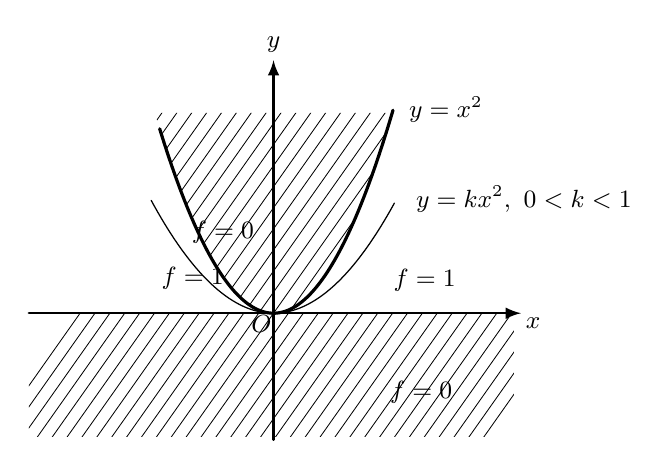
\begin{tikzpicture}[x=25.4pt, y=25.4pt, >=latex, line cap=round]
      % ---------- 上半阴影区域: y > x^2 (f = 0) ----------
      \begin{scope}
        \clip plot[domain=-1.688:1.688, samples=120] (\x, {\x*\x})
              -- (1.688, 2.85) -- (-1.688, 2.85) -- cycle;
        \foreach \c in {-6.0, -5.70, ..., 7.20} {
          \draw[line width=0.30pt] (-4.3, {1.417*(-4.3) + \c}) -- (4.3, {1.417*4.3 + \c});
        }
      \end{scope}
      % ---------- 下半阴影区域: y < 0 (f = 0) ----------
      \begin{scope}
        \clip (-3.48, -1.75) rectangle (3.42, 0);
        \foreach \c in {-6.0, -5.70, ..., 4.0} {
          \draw[line width=0.30pt] (-4.3, {1.417*(-4.3) + \c}) -- (4.3, {1.417*4.3 + \c});
        }
      \end{scope}
      % ---------- 坐标轴 ----------
      \draw[->, line width=0.9pt] (-3.48, 0) -- (3.52, 0) node[below right=-2pt] {\small $x$};
      \draw[->, line width=0.9pt] (0, -1.80) -- (0, 3.60) node[above=-1pt] {\small $y$};
      \node[below left=-1pt, inner sep=1.5pt] at (0, 0) {\small $O$};
      % ---------- 抛物线 y = x^2 (粗) 与 y = k x^2, 0<k<1 (细) ----------
      \draw[line width=1.15pt] plot[domain=-1.62:1.70, samples=120] (\x, {\x*\x});
      \draw[line width=0.45pt] plot[domain=-1.74:1.72, samples=120] (\x, {0.53*\x*\x});
      % ---------- 标注 ----------
      \node[inner sep=1pt] at (-1.15, 0.50) {\small $f = 1$};
      \node[inner sep=1pt] at (2.15, 0.47) {\small $f = 1$};
      \node[inner sep=1pt] at (-0.72, 1.15) {\small $f = 0$};
      \node[inner sep=1pt] at (2.10, -1.12) {\small $f = 0$};
      \node[anchor=west, inner sep=1pt] at (1.88, 2.90) {\small $y = x^{2}$};
      \node[anchor=west, inner sep=1pt] at (1.98, 1.62) {\small $y = kx^{2},\ 0 < k < 1$};
    \end{tikzpicture}
    \caption{}\label{fig:7.5.1}
  \end{figure}

  \item 证明:
  \[
    f(x, y) = \frac{1}{1 - xy}
  \]
  在 $D = [0, 1) \times [0, 1)$ 上连续, 但不一致连续.

  \item 设 $f(x, y)$ 定义在闭矩形 $[a, b] \times [c, d]$ 上. 如果 $f$ 对 $y$ 在 $[c, d]$ 上处处连续, 对 $x$ 在 $[a, b]$ (且关于 $y$!) 为一致连续. 证明: $f$ 在 $[a, b] \times [c, d]$ 上处处连续.

  \item (尤格定理) 设 $f$ 在 $\mathbb{R}^{2}$ 上分别对每一自变量 $x$ 与 $y$ 是连续的, 并且每当固定 $x$ 时 $f$ 对 $y$ 是单调的, 证明: $f$ 为 $\mathbb{R}^{2}$ 上的二元连续函数.

  \item 设 $\lim\limits_{y \to y_{0}} \varphi(y) = a$, $\lim\limits_{x \to x_{0}} \psi(x) = 0$, 且在 $(x_{0}, y_{0})$ 附近有 $|f(x, y) - \varphi(y)| \leqslant \psi(x)$. 证明:
  \[
    \lim_{(x, y) \to (x_{0}, y_{0})} f(x, y) = a.
  \]

  \item 设 $A$ 为 $(\mathbb{R}^{n}, \mathcal{T}_{\rho_{0}}^{n})$ 中的有界开集, $f\colon A \to \mathbb{R}$ 为一致连续的函数. 证明:

  \begin{tabular}{@{}p{0.45\linewidth}p{0.50\linewidth}@{}}
    (1) 可将 $f$ 延拓到 $\overline{A}$ 上; & (2) $f$ 在 $A$ 上有界.
  \end{tabular}

  \item 设 $u = \varphi(x, y)$ 与 $v = \psi(x, y)$ 在 $xy$ 平面中的点集 $A$ 上一致连续; $\varphi$ 与 $\psi$ 将点集 $A$ 映为 $uv$ 平面中的点集 $D$, $f(u, v)$ 在 $D$ 上一致连续. 证明: 复合函数 $f(\varphi(x, y), \psi(x, y))$ 在 $A$ 上一致连续.

  \item 设 $(\mathbb{R}^{n}, \mathcal{T}_{\rho_{0}}^{n})$ 为 $n$ 维 Euclid 空间, $f\colon \mathbb{R}^{n} \to \mathbb{R}^{1}$ 为连续函数, $\alpha \in \mathbb{R}$,
  \[
    E = \left\{x = (x_{1}, x_{2}, \cdots, x_{n}) \mid f(x) = f(x_{1}, x_{2}, \cdots, x_{n}) > \alpha\right\} \subset \mathbb{R}^{n},
  \]
  \[
    F = \left\{x = (x_{1}, x_{2}, \cdots, x_{n}) \mid f(x) = f(x_{1}, x_{2}, \cdots, x_{n}) \geqslant \alpha\right\} \subset \mathbb{R}^{n}.
  \]
  证明: $E$ 为 $(\mathbb{R}^{n}, \mathcal{T}_{\rho_{0}}^{n})$ 中的开集, $F$ 为 $(\mathbb{R}^{n}, \mathcal{T}_{\rho_{0}}^{n})$ 中的闭集.

  \item 设 $f(x, y) = \dfrac{1}{xy}$, $r = \sqrt{x^{2} + y^{2}}$, $k > 1$,
  \[
    D_{1} = \left\{(x, y)\ \middle|\ \frac{x}{k} \leqslant y \leqslant kx\right\},
  \]
  \[
    D_{2} = \{(x, y) \mid x > 0,\ y > 0\}.
  \]
  试分别讨论 $i = 1, 2$ 时极限 $\lim\limits_{\substack{(x, y) \in D_{i} \\ r \to +\infty}} f(x, y)$ 是否存在? 并说明理由.

  \item 设 $f(t)$ 在开区间 $(a, b)$ 内连续可导, 在开区间 $D = (a, b) \times (a, b)$ 内定义函数
  \[
    F(x, y) =
    \begin{cases}
      \dfrac{f(x) - f(y)}{x - y}, & x \neq y, \\[2.5mm]
      f'(x), & x = y.
    \end{cases}
  \]
  证明: $\forall c \in (a, b)$, 有 $\lim\limits_{(x, y) \to (c, c)} F(x, y) = f'(c)$.

  \item 设 $\varphi(x)$ 在 $[a, b]$ 上连续, 令 $f(x, y) = \varphi(x)$, $(x, y) \in D = [a, b] \times (-\infty, +\infty)$. 证明: $f$ 在 $D$ 上连续且为一致连续函数.

  \item 设 $f$ 在 $\mathbb{R}^{2}$ 上连续, 且 $\lim\limits_{r \to +\infty} f(x, y) = a$, $r = \sqrt{x^{2} + y^{2}}$. 证明:

  \begin{tabular}{@{}p{0.45\linewidth}p{0.50\linewidth}@{}}
    (1) $f$ 在 $\mathbb{R}^{2}$ 上有界; & (2) $f$ 在 $\mathbb{R}^{2}$ 上一致连续.
  \end{tabular}

  \item 叙述并证明二元函数的局部保号性.

  \item 设 $E$ 与 $F$ 为度量空间 $(X, \mathcal{T})$ 中的两个不相交的闭集. 证明:
  (1) $U_{E} = \{x \mid \rho(x, E) < \rho(x, F)\} \subset X$ 与 $U_{F} = \{x \mid \rho(x, E) > \rho(x, F)\} \subset X$ 分别为 $E$ 与 $F$ 的两个不相交的开邻域;
  (2) $U_{E} = \bigcup\limits_{x \in E} B\left(x; \dfrac{1}{3}\rho(x, F)\right)$ 与 $U_{F} = \bigcup\limits_{x \in F} B\left(x; \dfrac{1}{3}\rho(x, E)\right)$ 分别为 $E$ 与 $F$ 的两个不相交的开邻域.

  \item 设 $(X, \rho)$ 为度量空间, $A \neq \varnothing$ 且 $A \subset X$, 则 $f\colon X \to \mathbb{R}$, $f(x) = \rho(x, A)$ 为 $X$ 上的一致连续函数.

  \item 设函数 $f(x, y)$ 在 $[a, A] \times [b, B]$ 上连续, 而函数列 $\{\varphi_{n}(x)\}$ 在 $[a, A]$ 上一致收敛, 且 $b \leqslant \varphi_{n}(x) \leqslant B$, $n \in \mathbb{Z}_{+}$. 证明: 函数列 $\{F_{n}(x)\} = \{f(x, \varphi_{n}(x))\}$ 也在 $[a, A]$ 上一致收敛.

  \item 设 (1) 函数 $f(x, y)$ 于 $(a, A) \times (b, B)$ 内是连续的; (2) 函数 $\varphi(x)$ 于区间 $(a, A)$ 内连续且 $b < \varphi(x) < B$. 证明: 函数
  \[
    F(x) = f(x, \varphi(x))
  \]
  在区间 $(a, A)$ 内是连续的.

  \item 设 (1) 函数 $f(x, y)$ 于 $(a, A) \times (b, B)$ 内是连续的; (2) 函数 $x = \varphi(u, v)$, $y = \psi(u, v)$ 在 $(a', A') \times (b', B')$ 内是连续的, 并分别有属于 $(a, A)$ 与 $(b, B)$ 的值. 证明: 函数
  \[
    F(u, v) = f(\varphi(u, v), \psi(u, v))
  \]
  在 $(a', A')$ 内连续.

  \item 设 $(u, v) = F(x, y) = (f(x, y), g(x, y))$, 其中
  \[
    u = f(x, y) =
    \begin{cases}
      \dfrac{x}{(x^{2} + y^{2})^{\alpha}}\ln(|x| + |y|), & x^{2} + y^{2} \neq 0, \\[2.5mm]
      0, & x^{2} + y^{2} = 0;
    \end{cases}
  \]
  \[
    v = g(x, y) =
    \begin{cases}
      \dfrac{y}{(x^{2} + y^{2})^{\alpha}}\ln(|x| + |y|), & x^{2} + y^{2} \neq 0, \\[2.5mm]
      0, & x^{2} + y^{2} = 0.
    \end{cases}
  \]
  讨论 $F(x, y)$ 的连续性.
\end{exblock}

% ==================================================================
%  复习题 7
%  源：徐森林、薛春华《数学分析》第二册，印刷页 52-53 (PDF p. 58-59)
%  底本：PaddleOCR-VL-1.6 JSON/MD 识别结果，人工逐字核校与公式精修
%  规范：全西文标点，忠实原文条目编号与推导
% ==================================================================

\begin{exblock}{复习题 7}
  \item (杨忠道定理) 拓扑空间 $(X, \mathcal{T})$ 的任一子集 $A$ 的导集 $A'$ 为闭集 $\iff$ $(X, \mathcal{T})$ 的每个独点集的导集为闭集.

  \item 设 $(X, \mathcal{T})$ 为拓扑空间, $\{A_{\alpha} \mid \alpha \in \Gamma\}$ 为 $X$ 中的一个子集族, 如果 $\forall \alpha \in \Gamma$, 导集 $A_{\alpha}'$ 为 $(X, \mathcal{T})$ 中的闭集, 则集合 $\left(\bigcup\limits_{\alpha \in \Gamma} A_{\alpha}'\right)'$ 也为闭集.

  \item (1) 证明: $(\mathbb{R}^{n}, \mathcal{T}_{\rho_{0}}^{n})$ 中至多可数个稠密开集的交为 $(\mathbb{R}^{n}, \mathcal{T}_{\rho_{0}}^{n})$ 中的稠密开集;

  (2) 一般的度量空间 $(X, \mathcal{T}_{\rho})$, 上述结论仍正确吗?

  \item 设 $Y$, $Y_{\alpha}$ ($\alpha \in \Gamma$) 都是拓扑空间 $(X, \mathcal{T})$ 的连通子集. 如果 $\forall \alpha \in \Gamma$, $Y_{\alpha} \cap Y \neq \varnothing$, 则 $\left(\bigcup\limits_{\alpha \in \Gamma} Y_{\alpha}\right) \cup Y$ 为 $(X, \mathcal{T})$ 的连通子集. 上述「连通」改为「道路连通」结论如何? 并说明理由.

  \item 设 $\{Y_{\alpha} \mid \alpha \in \Gamma\}$ 为拓扑空间 $(X, \mathcal{T})$ 的道路连通的子集族, 并且满足: $\forall \alpha, \beta \in \Gamma$, 存在 $\Gamma$ 中的有限个元素 $\gamma_{1} = \alpha$, $\gamma_{2}$, $\cdots$, $\gamma_{n+1} = \beta$, 使得 $Y_{\gamma_{i}} \cap Y_{\gamma_{i+1}} \neq \varnothing$, $i = 1, 2, \cdots, n$, 则 $\bigcup\limits_{\alpha \in \Gamma} Y_{\alpha}$ 为道路连通子集. 上述「道路连通」改为「连通」结论如何? 并说明理由.

  \item 证明: 满足 $A_{1}$ 的可数紧致空间必为序列紧致空间.

  \item 举例说明拓扑空间中两个紧致子集的交可以不为紧致子集.

  \item 设 $(X, \rho)$ 为列紧度量空间, 则 $\forall \varepsilon > 0$, $X$ 必有 $\varepsilon$ 网 $A$ (即 $A$ 为 $X$ 的有限子集, 并且 $\forall x \in X$, 有 $\rho(x, A) = \inf\limits_{y \in A} \rho(y, x) < \varepsilon$).

  \item 设 $(X, \rho)$ 为度量空间, 证明:
  \[
    (X, \mathcal{T}_{\rho})\ \text{紧致} \iff (X, \mathcal{T}_{\rho})\ \text{列紧}.
  \]
  (提示: 应用 Lebesgue 数定理与本复习题第 8 题证明其充分性.)

  \item 设函数 $z = f(x, y)$ 在 $D = [0, 1] \times [0, 1]$ 上有定义, 且 $\forall x_{0} \in [0, 1]$, $f(x, y)$ 于 $(x_{0}, 0)$ 点连续, 证明: $\exists \delta > 0$, s. t. $f(x, y)$ 于 $D^{*} = \{(x, y) \mid 0 \leqslant x \leqslant 1,\ 0 \leqslant y \leqslant \delta\} = [0, 1] \times [0, \delta]$ 上有界.

  \item (1) 设 $u = f(x, y, z)$ 在闭立方体 $[a, b]^{3}$ 上连续, 证明: $g(x, y) = \max\limits_{a \leqslant z \leqslant b} f(x, y, z)$ 在正方形 $[a, b]^{2} \subset \mathbb{R}^{2}$ 上连续;

  (2) 设 $f(x, y, z)$ 在 $[a, b]^{3} = [a, b] \times [a, b] \times [a, b]$ 上连续, 令
  \[
    g(x) = \max_{a \leqslant y \leqslant x} \min_{a \leqslant z \leqslant b} f(x, y, z).
  \]
  证明: $g(x)$ 在 $[a, b]$ 上连续.

  \item 设 $U$ 为拓扑空间 $(X, \mathcal{T})$ 中的一个开集. $\mathcal{A}$ 为 $(X, \mathcal{T})$ 中的一个由紧致闭集构成的集族. 如果 $\mathcal{A}$ 满足 $\bigcap\limits_{A \in \mathcal{A}} A \subset U$, 则存在 $\mathcal{A}$ 的一个有限子族 $\{A_{1}, A_{2}, \cdots, A_{n}\}$ 也满足
  \[
    A_{1} \cap A_{2} \cap \cdots \cap A_{n} \subset U.
  \]

  \item 设 $(X, \mathcal{T})$ 为一个 Hausdorff 空间, $\mathcal{A}$ 为 $(X, \mathcal{T})$ 中由紧致子集构成的非空集族. 证明: 如果 $\mathcal{A}$ 中任意有限个元素的交是连通的, 则这个集族的交 $\bigcap\limits_{A \in \mathcal{A}} A$ 也是连通的.

  \item 设 $f(x, y)$ 满足: (1) 对固定的 $y \neq b$, $\lim\limits_{x \to a} f(x, y) = \psi(y)$; (2) $\exists \eta > 0$, s. t. $f(x, y)$ 当 $y \to b$ 时关于 $x \in E = \{x \mid 0 < |x - a| < \eta\}$ 存在一致极限 $\varphi(x)$. 证明:
  \[
    \lim_{x \to a} \lim_{y \to b} f(x, y) = \lim_{y \to b} \lim_{x \to a} f(x, y).
  \]

  \item 设 $f_{0}(x)$ 在 $[a, b]$ 上连续, $g(x, y)$ 在闭区域 $[a, b]^{2} = [a, b] \times [a, b]$ 上连续. 对任何 $x \in [a, b]$, 令
  \[
    f_{n}(x) = \int_{a}^{x} g(x, y)f_{n-1}(y)\,\mathrm{d}y, \quad n = 1, 2, \cdots.
  \]
  证明: 函数列 $\{f_{n}(x)\}$ 在 $[a, b]$ 上一致收敛于 $0$.

  \item 设有界点列 $\boldsymbol{z}^{n} = (x_{n}, y_{n})$, $n = 1, 2, \cdots$, 满足:
  \[
    \varliminf_{n \to +\infty} \|\boldsymbol{z}^{n}\| = l, \quad \varlimsup_{n \to +\infty} \|\boldsymbol{z}^{n}\| = L, \quad l < L,
  \]
  \[
    \lim_{n \to +\infty} \|\boldsymbol{z}^{n+1} - \boldsymbol{z}^{n}\| = 0.
  \]
  证明: 对 $\forall \mu \in (l, L)$, 圆周 $x^{2} + y^{2} = \mu^{2}$ 上至少有 $\{\boldsymbol{z}^{n}\}$ 的一个聚点.
\end{exblock}



% 第 8 章（进行中）
% ==================================================================
%  徐森林、薛春华《数学分析》（第二册）
%  第 8 章  n 元函数微分学
% ==================================================================

\chapter{\texorpdfstring{$n$}{n} 元函数微分学}\label{ch:8}

本章引进方向导数与偏导数, 并用偏导数表达方向导数; 给出了复合函数的求导链规则. 作为它的应用, 证明在区域 $U$ 上, 如果 $\left.\dfrac{\partial f}{\partial x_{i}}\right|_{U} \equiv 0\ (i = 1, 2, \cdots, n)$, $f$ 在 $\overline{U}$ 上连续, 则 $f$ 为常值函数. 接着详细讨论了函数可微与映射可微的重要概念, 得到了可微的充分条件和必要条件, 以及函数的高维微分中值定理与映射的拟微分中值定理. $n$ 元 Lagrange 型余项的 Taylor 公式与 Peano 型余项的 Taylor 公式是 $n$ 元微分学的重要定理. Peano 型余项 Taylor 公式的惟一性定理保证了用各种方法 Taylor 展开的合法性. Lagrange 型余项的 Taylor 公式在第 9 章极值研究中起到重要作用. 最后, 隐射 (隐函数) 与逆映 (反函数) 定理的两种精美的证明, 使读者得到了分析能力的严格训练. 这些知识在第 9 章参数曲面与条件极值研究中有重要应用.

% ==================================================================
%  §8.1  方向导数与偏导数
%  源：徐森林、薛春华《数学分析》第二册，印刷页 54-69 (PDF p. 60-75)
%  底本：PaddleOCR-VL-1.6 JSON/MD 识别结果，人工逐字核校与公式精修
%  规范：全西文标点，忠实原文定义、注、定理、例题、练习题编号与推导
% ==================================================================

\section{方向导数与偏导数}\label{sec:8.1}

对一元函数 $y = f(x)$, 如果极限
\[
  \lim_{t \to 0}\frac{f(x_{0} + t) - f(x_{0})}{t} = \lim_{\Delta x \to 0}\frac{f(x_{0} + \Delta x) - f(x_{0})}{\Delta x} = \lim_{x \to x_{0}}\frac{f(x) - f(x_{0})}{x - x_{0}}
\]
存在有限, 则 $f$ 在 $x_{0}$ 处可导, 且上述极限就是 $f$ 在 $x_{0}$ 处的导数 $f'(x_{0}) = \dfrac{\mathrm{d}f}{\mathrm{d}x}\Big|_{x = x_{0}} = \dfrac{\mathrm{d}y}{\mathrm{d}x}\Big|_{x = x_{0}} = y'(x_{0})$, 它是 $f$ 在 $x_{0}$ 处的变化率.

$f$ 在 $x_{0}$ 处可导 $\iff f$ 在 $x_{0}$ 处的左、右导数相等, 即
\[
  f_{-}'(x_{0}) = \lim_{x \to x_{0}^{-}}\frac{f(x) - f(x_{0})}{x - x_{0}} = \lim_{x \to x_{0}^{+}}\frac{f(x) - f(x_{0})}{x - x_{0}} = f_{+}'(x_{0}).
\]

在 $\mathbb{R}^{n}\ (n \geqslant 2)$ 中, 一个点的开邻域中过该点不只是两个方向, 而是有无穷多个方向. 因此, 代替左、右导数应考虑方向导数.

\begin{definition}\label{def:8.1.1}
设 $U \subset \mathbb{R}^{n}$ 为开集 (今后都指 Euclid 空间 $(\mathbb{R}^{n}, \mathcal{T}_{\rho_{0}}^{n})$ 中的开集), $f: U \to \mathbb{R}^{1}$, $\boldsymbol{e}$ 为 $\mathbb{R}^{n}$ 中的一个单位向量, $\boldsymbol{x}^{0} \in U$, 令
\[
  u(t) = f(\boldsymbol{x}^{0} + t\boldsymbol{e})
\]
(此时 $u$ 为 $t$ 的一元函数). 如果 $u$ 在 $t = 0$ 的导数
\[
  u'(0) = \lim_{t \to 0}\frac{u(t) - u(0)}{t} = \lim_{t \to 0}\frac{f(\boldsymbol{x}^{0} + t\boldsymbol{e}) - f(\boldsymbol{x}^{0})}{t}
\]
存在有限, 则称它为 $f$ 在点 $\boldsymbol{x}^{0}$ 沿方向 $\boldsymbol{e}$ 的\textbf{方向导数}, 记作 $\dfrac{\partial f}{\partial \boldsymbol{e}}(\boldsymbol{x}^{0})$, 它就是 $f$ 在点 $\boldsymbol{x}^{0}$ 沿方向 $\boldsymbol{e}$ 的变化率 (\cref{fig:8.1.1}), 且 $\tan\theta = \dfrac{\partial f}{\partial \boldsymbol{e}}(\boldsymbol{x}^{0})$.
\end{definition}

\begin{figure}[htbp]
  \centering
  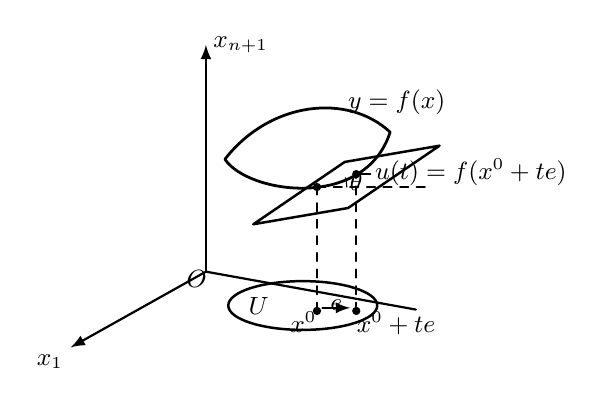
\begin{tikzpicture}[x=0.86cm, y=0.86cm, >=latex, line cap=round, line join=round]
    % ---------- 坐标架 ----------
    \draw[line width=0.8pt, ->] (0, 0) -- (-2.00, -1.12) node[below left=-1pt] {\small $x_{1}$};
    \draw[line width=0.8pt, ->] (0, 0) -- (0, 3.35) node[right=-1pt] {\small $x_{n+1}$};
    \draw[line width=0.8pt] (0, 0) -- (3.10, -0.56);
    \node[below left=-1.5pt, inner sep=1pt] at (0, 0) {\small $O$};
    % ---------- 底面区域 U ----------
    \draw[line width=0.9pt] (1.43, -0.50) ellipse (1.10 and 0.36);
    \node[inner sep=1pt] at (0.78, -0.50) {\small $U$};
    \fill (1.64, -0.58) circle (1.5pt);
    \node[below left=-1.5pt, inner sep=1.5pt] at (1.64, -0.58) {\small $x^{0}$};
    \fill (2.22, -0.58) circle (1.5pt);
    \node[below right=-1.5pt, inner sep=1.5pt] at (2.22, -0.58) {\small $x^{0}+te$};
    \draw[->, line width=0.8pt] (1.72, -0.535) -- (2.13, -0.535);
    \node[above=-2pt, inner sep=1pt] at (1.925, -0.54) {\small $e$};
    % ---------- 竖直虚线与曲面片 ----------
    \draw[line width=0.7pt, dashed] (1.64, -0.58) -- (1.64, 1.25);
    \draw[line width=0.7pt, dashed] (2.22, -0.58) -- (2.22, 1.44);
    % 曲面片 y = f(x)：「透镜」轮廓（下缘经过 A、B）
    \draw[line width=1.0pt]
      (0.28, 1.66)
      .. controls (0.95, 2.52) and (2.10, 2.64) .. (2.72, 2.06)
      .. controls (2.35, 0.90) and (0.62, 1.15) .. (0.28, 1.66);
    \node[anchor=west, inner sep=1pt] at (2.05, 2.50) {\small $y = f(\boldsymbol{x})$};
    % 曲面上的点 A(x^0) 与 B(x^0+te)
    \fill (1.64, 1.25) circle (1.5pt);
    \fill (2.22, 1.44) circle (1.5pt);
    \node[anchor=west, inner sep=1pt] at (2.45, 1.47) {\small $u(t) = f(\boldsymbol{x}^{0} + t\boldsymbol{e})$};
    \draw[line width=0.5pt] (2.43, 1.44) -- (2.24, 1.44);
    % 平面（由 e 方向与竖直方向张成的平行四边形）
    \draw[line width=0.9pt] (0.70, 0.70) -- (2.10, 0.94) -- (3.45, 1.86) -- (2.05, 1.62) -- cycle;
    % 过 A 的水平虚线 与 夹角 theta
    \draw[line width=0.7pt, dashed] (1.64, 1.25) -- (3.25, 1.25);
    \draw (2.08, 1.25) arc[start angle=0, end angle=18.1, radius=0.44];
    \node[inner sep=1pt] at (2.22, 1.33) {\small $\theta$};
  \end{tikzpicture}
  \caption{}\label{fig:8.1.1}
\end{figure}

\begin{example}\label{ex:8.1.1}
设 $\boldsymbol{e}$ 为一个方向, 则 $\|-\boldsymbol{e}\| = \|\boldsymbol{e}\| = 1$, 可见 $-\boldsymbol{e}$ 也为一个方向. 此时, 我们有
\begin{align*}
  \frac{\partial f}{\partial(-\boldsymbol{e})}(\boldsymbol{x}^{0})
  &= \lim_{t \to 0}\frac{f(\boldsymbol{x}^{0} + t(-\boldsymbol{e})) - f(\boldsymbol{x}^{0})}{t}
   = -\lim_{-t \to 0}\frac{f(\boldsymbol{x}^{0} + (-t)\boldsymbol{e}) - f(\boldsymbol{x}^{0})}{-t} \\
  &= -\frac{\partial f}{\partial \boldsymbol{e}}(\boldsymbol{x}^{0}).
\end{align*}
\end{example}

\begin{example}\label{ex:8.1.2}
考察二元函数
\[
  f(x, y) = \begin{cases}
    \dfrac{2xy}{x^{2} + y^{2}}, & (x, y) \neq (0, 0), \\[2.5mm]
    1, & (x, y) = (0, 0).
  \end{cases}
\]
记方向 $\boldsymbol{e} = (\cos\theta, \sin\theta)$, $0 \leqslant \theta < 2\pi$, 并取 $\boldsymbol{x}^{0} = (0, 0)$, 当 $t \neq 0$ 时有
\[
  \frac{f(\boldsymbol{x}^{0} + t\boldsymbol{e}) - f(\boldsymbol{x}^{0})}{t} = \frac{f(t\cos\theta, t\sin\theta) - f(0, 0)}{t} = \frac{2\cos\theta\sin\theta - 1}{t} = \frac{\sin 2\theta - 1}{t}.
\]
由此看出, 当且仅当 $\theta = \dfrac{\pi}{4}$ 与 $\dfrac{5\pi}{4}$, 方向导数存在且为零. 而对其他 $\theta$, 方向导数不存在.
\[
  \begin{aligned}
    \frac{\partial f}{\partial \boldsymbol{e}}(\boldsymbol{x}^{0})
    &= \lim_{t \to 0}\frac{f(\boldsymbol{x}^{0} + t\boldsymbol{e}) - f(\boldsymbol{x}^{0})}{t} = \lim_{t \to 0}\frac{\sin 2\theta - 1}{t} \\
    &= \begin{cases}
         0, & \theta = \dfrac{\pi}{4}\ \text{与}\ \dfrac{5\pi}{4}, \\[3.5mm]
         \infty, & \theta \in \left[0, \dfrac{\pi}{4}\right) \bigcup \left(\dfrac{\pi}{4}, \dfrac{5\pi}{4}\right) \bigcup \left(\dfrac{5\pi}{4}, 2\pi\right).
       \end{cases}
  \end{aligned} \qedhere
\]
\end{example}

记 $\boldsymbol{e}_{i} = (0, 0, \cdots, 0, \underset{\text{第 } i \text{ 个}}{1}, 0, \cdots, 0)$ 为 $\mathbb{R}^{n}$ 中的规范正交基, 即
\[
  \langle \boldsymbol{e}_{i}, \boldsymbol{e}_{j} \rangle = \delta_{ij} = \begin{cases} 1, & i = j, \\ 0, & i \neq j. \end{cases}
\]
设 $\boldsymbol{x}^{0} = (x_{1}^{0}, x_{2}^{0}, \cdots, x_{n}^{0})$, 则
\[
  \begin{aligned}
    \frac{\partial f}{\partial \boldsymbol{e}_{i}}(\boldsymbol{x}^{0})
    &= \lim_{t \to 0}\frac{f(\boldsymbol{x}^{0} + t\boldsymbol{e}_{i}) - f(\boldsymbol{x}^{0})}{t} \\
    &= \lim_{t \to 0}\frac{f(x_{1}^{0}, x_{2}^{0}, \cdots, x_{i-1}^{0}, x_{i}^{0} + t, x_{i+1}^{0}, \cdots, x_{n}^{0}) - f(x_{1}^{0}, x_{2}^{0}, \cdots, x_{n}^{0})}{t} \\
    &= \lim_{x_{i} \to x_{i}^{0}}\frac{f(x_{1}^{0}, x_{2}^{0}, \cdots, x_{i-1}^{0}, x_{i}, x_{i+1}^{0}, \cdots, x_{n}^{0}) - f(x_{1}^{0}, x_{2}^{0}, \cdots, x_{n}^{0})}{x_{i} - x_{i}^{0}} \\
    &\reason{记作} \frac{\partial f}{\partial x_{i}}(\boldsymbol{x}^{0}) = f_{x_{i}}'(\boldsymbol{x}^{0}) = f_{i}'(\boldsymbol{x}^{0}),
  \end{aligned}
\]
称它为 $f$ 的第 $i$ 个\textbf{一阶偏导数}, 它是 $\boldsymbol{x}^{0}$ 点处沿 $\boldsymbol{e}_{i}$ 方向的方向导数.

\begin{example}\label{ex:8.1.3}
在 $\mathbb{R}^{n}$ 中计算函数 $f(\boldsymbol{x}) = \|\boldsymbol{x}\| = \sqrt{x_{1}^{2} + x_{2}^{2} + \cdots + x_{n}^{2}}$ 的偏导数, 其中 $\boldsymbol{x} = (x_{1}, x_{2}, \cdots, x_{n})$.

\begin{solution}
当 $\boldsymbol{x} \neq \boldsymbol{0}$ 时,
\[
  f_{x_{i}}'(\boldsymbol{x}) = \frac{1}{2}(x_{1}^{2} + x_{2}^{2} + \cdots + x_{n}^{2})^{-\frac{1}{2}} \cdot 2x_{i} = \frac{x_{i}}{\|\boldsymbol{x}\|}, \quad i = 1, 2, \cdots, n.
\]
当 $\boldsymbol{x} = \boldsymbol{0}$ 时, 设 $\boldsymbol{e}$ 为任一给定的方向 (单位向量), 此时, 极限
\[
  \lim_{t \to 0}\frac{f(t\boldsymbol{e}) - f(\boldsymbol{0})}{t} = \lim_{t \to 0}\frac{\|t\boldsymbol{e}\|}{t} = \lim_{t \to 0}\frac{|t|\,\|\boldsymbol{e}\|}{t} = \lim_{t \to 0}\frac{|t|}{t}
\]
不存在, 即 $f$ 在原点处的任何方向导数都不存在. 特别地, $f$ 在原点处的任何偏导数也不存在.\qedhere
\end{solution}
\end{example}

如果在开集 $U$ 中的每一点有偏导数, 就得到 $n$ 个一阶偏导函数
\[
  \frac{\partial f}{\partial \boldsymbol{e}_{i}} = \frac{\partial f}{\partial x_{i}}, \quad i = 1, 2, \cdots, n.
\]
如果 $f$ 的一阶偏导函数 $\dfrac{\partial f}{\partial x_{i}}$ 又有偏导数, 称为 $f$ 的\textbf{二阶偏导数}, 记作
\[
  f_{x_{i}x_{j}}'' = \frac{\partial^{2}f}{\partial x_{i}\partial x_{j}} = \frac{\partial}{\partial x_{j}}\Big(\frac{\partial f}{\partial x_{i}}\Big),
\]
\[
  f_{x_{i}x_{i}}'' = \frac{\partial^{2}f}{\partial x_{i}^{2}} = \frac{\partial}{\partial x_{i}}\Big(\frac{\partial f}{\partial x_{i}}\Big), \quad i, j = 1, 2, \cdots, n.
\]
类似可定义 $3$ 阶, $4$ 阶, $\cdots$, $m$ 阶, $\cdots$ 偏导数.

$f$ 为 $C^{k}$ 函数, 即

\noindent $k = 0$, $f$ 连续;

\noindent $0 < k < +\infty$, $f$ 在 $U$ 中有直至 $k$ 阶连续偏导数;

\noindent $k = \infty$, $f$ 在 $U$ 中有各阶连续的偏导数;

\noindent $k = \omega$, $f$ 在 $U$ 中是\textbf{实解析}的, 即 $f$ 在 $U$ 中每一点邻近可展开为收敛的 ($n$ 元) 幂级数:
\[
  f(x_{1}, x_{2}, \cdots, x_{n}) = \sum_{k = 0}^{\infty}\sum_{j_{1}, j_{2}, \cdots, j_{k} = 1}^{n} a_{j_{1}j_{2}\cdots j_{k}}(x_{j_{1}}^{0} - x_{j_{1}})(x_{j_{2}}^{0} - x_{j_{2}})\cdots(x_{j_{k}}^{0} - x_{j_{k}}).
\]
记 $C^{k}(U, \mathbb{R}^{1})$ 为从 $U$ 到 $\mathbb{R}^{1}$ 的 $C^{k}$ 函数的全体.

\begin{theorem}\label{thm:8.1.1}
设 $U \subset \mathbb{R}^{2}$ 为开集, $f: U \to \mathbb{R}^{1}$ 为二元函数. 如果 $f_{xy}''$ 与 $f_{yx}''$ 在 $(x_{0}, y_{0}) \in U$ 连续, 则
\[
  f_{xy}''(x_{0}, y_{0}) = f_{yx}''(x_{0}, y_{0}).
\]
\end{theorem}

\begin{proof}
当 $k \neq 0$, $h \neq 0$ 时, 分别对
\[
  \varphi(y) = f(x_{0} + h, y) - f(x_{0}, y)
\]
与
\[
  \psi(x) = f(x, y_{0} + k) - f(x, y_{0})
\]
应用 Lagrange 中值定理, 就有
\begin{align*}
  &\ [f(x_{0} + h, y_{0} + k) - f(x_{0}, y_{0} + k)] - [f(x_{0} + h, y_{0}) - f(x_{0}, y_{0})] \\
  ={} &\ \varphi(y_{0} + k) - \varphi(y_{0}) = \varphi'(y_{0} + \theta_{1}k)k \\
  ={} &\ [f_{y}'(x_{0} + h, y_{0} + \theta_{1}k) - f_{y}'(x_{0}, y_{0} + \theta_{1}k)]k \\
  ={} &\ f_{yx}''(x_{0} + \theta_{2}h, y_{0} + \theta_{1}k)hk, \quad 0 < \theta_{1}, \theta_{2} < 1.
\end{align*}
另一方面
\begin{align*}
  &\ [f(x_{0} + h, y_{0} + k) - f(x_{0}, y_{0} + k)] - [f(x_{0} + h, y_{0}) - f(x_{0}, y_{0})] \\
  ={} &\ [f(x_{0} + h, y_{0} + k) - f(x_{0} + h, y_{0})] - [f(x_{0}, y_{0} + k) - f(x_{0}, y_{0})] \\
  ={} &\ \psi(x_{0} + h) - \psi(x_{0}) = \psi'(x_{0} + \theta_{3}h)h \\
  ={} &\ [f_{x}'(x_{0} + \theta_{3}h, y_{0} + k) - f_{x}'(x_{0} + \theta_{3}h, y_{0})]h \\
  ={} &\ f_{xy}''(x_{0} + \theta_{3}h, y_{0} + \theta_{4}k)hk, \quad 0 < \theta_{3}, \theta_{4} < 1.
\end{align*}
因此
\[
  f_{xy}''(x_{0} + \theta_{3}h, y_{0} + \theta_{4}k) = f_{yx}''(x_{0} + \theta_{2}h, y_{0} + \theta_{1}k).
\]
由于 $f_{xy}''$ 与 $f_{yx}''$ 在 $(x_{0}, y_{0})$ 处连续, 令 $h \to 0$, $k \to 0$ 就得到
\[
  f_{xy}''(x_{0}, y_{0}) = f_{yx}''(x_{0}, y_{0}). \qedhere
\]
\end{proof}

应用\cref{thm:8.1.1}及归纳法立即可得下面定理.

\begin{theoremp}\label{thm:8.1.1p}
$U \subset \mathbb{R}^{n}$ 为开集, $f: U \to \mathbb{R}^{1}$ 为 $n$ 元函数. 如果 $f$ 在 $U$ 上有直至 $k$ 阶的偏导数, 且都在 $\boldsymbol{x}^{0} = (x_{1}^{0}, x_{2}^{0}, \cdots, x_{n}^{0}) \in U$ 连续, 则
\[
  \frac{\partial^{l}f}{\partial x_{i_{1}}\partial x_{i_{2}}\cdots\partial x_{i_{l}}}(\boldsymbol{x}^{0}) = \frac{\partial^{l}f}{\partial x_{i_{2}}\partial x_{i_{1}}\cdots\partial x_{i_{l}}}(\boldsymbol{x}^{0}) = \cdots = \frac{\partial^{l}f}{\partial x_{i_{l}}\partial x_{i_{l-1}}\cdots\partial x_{i_{1}}}(\boldsymbol{x}^{0}),
\]
即任一 $l\ (\leqslant k)$ 阶偏导数与逐次求导的次序无关.
\end{theoremp}

如果\cref{thm:8.1.1}中条件 ``$f_{xy}''$ 与 $f_{yx}''$ 在 $(x_{0}, y_{0})$ 连续'' 不满足, 则其结论 ``$f_{xy}''(x_{0}, y_{0}) = f_{yx}''(x_{0}, y_{0})$'' 不一定成立.

\begin{example}\label{ex:8.1.4}
设
\[
  f(x, y) = \begin{cases}
    xy\dfrac{x^{2} - y^{2}}{x^{2} + y^{2}}, & (x, y) \neq (0, 0), \\[2.5mm]
    0, & (x, y) = (0, 0),
  \end{cases}
\]
则有
\[
  f_{x}'(0, 0) = \lim_{x \to 0}\frac{f(x, 0) - f(0, 0)}{x - 0} = \lim_{x \to 0}\frac{0 - 0}{x} = \lim_{x \to 0}0 = 0,
\]
\[
  f_{y}'(0, 0) = \lim_{y \to 0}\frac{f(0, y) - f(0, 0)}{y - 0} = \lim_{y \to 0}\frac{0 - 0}{y} = \lim_{y \to 0}0 = 0.
\]
当 $(x, y) \neq (0, 0)$ 时,
\[
  f_{x}'(x, y) = y\left[\frac{x^{2} - y^{2}}{x^{2} + y^{2}} + \frac{4x^{2}y^{2}}{(x^{2} + y^{2})^{2}}\right],
\]
\[
  f_{y}'(x, y) = x\left[\frac{x^{2} - y^{2}}{x^{2} + y^{2}} - \frac{4x^{2}y^{2}}{(x^{2} + y^{2})^{2}}\right].
\]
于是, $\forall y$, $f_{x}'(0, y) = -y$, $f_{xy}''(0, 0) = -1$; $\forall x$, $f_{y}'(x, 0) = x$, $f_{yx}''(0, 0) = 1$,
\[
  f_{xy}''(0, 0) \neq f_{yx}''(0, 0).
\]
由此与\cref{thm:8.1.1}可知, $f_{xy}''$ 与 $f_{yx}''$ 在 $(0, 0)$ 至少有一个不连续.
\end{example}

\begin{example}\label{ex:8.1.5}
设 $f(x, y) = xy$, 求 $f$ 在点 $\boldsymbol{x}^{0} = (1, 1)$ 沿方向 $\boldsymbol{e} = \left(\dfrac{1}{\sqrt{2}}, \dfrac{1}{\sqrt{2}}\right)$ 的方向导数.

\begin{solution}[解法 1]
\[
  \frac{f(\boldsymbol{x}^{0} + t\boldsymbol{e}) - f(\boldsymbol{x}^{0})}{t} = \frac{f\left(1 + \dfrac{t}{\sqrt{2}}, 1 + \dfrac{t}{\sqrt{2}}\right) - f(1, 1)}{t} = \frac{\left(1 + \dfrac{t}{\sqrt{2}}\right)^{2} - 1^{2}}{t} = \sqrt{2} + \frac{t}{2},
\]
\[
  \frac{\partial f}{\partial \boldsymbol{e}}(1, 1) = \lim_{t \to 0}\left(\sqrt{2} + \frac{t}{2}\right) = \sqrt{2}.
\]
\end{solution}

\begin{solution}[解法 2]
\begin{align*}
  \frac{\partial f}{\partial \boldsymbol{e}}(1, 1)
  &= \lim_{t \to 0}\frac{f(\boldsymbol{x}^{0} + t\boldsymbol{e}) - f(\boldsymbol{x}^{0})}{t} \\
  &\reason{\cref{thm:8.1.5}} f_{x}'(1, 1) \cdot \frac{1}{\sqrt{2}} + f_{y}'(1, 1) \cdot \frac{1}{\sqrt{2}} \\
  &= 1 \times \frac{1}{\sqrt{2}} + 1 \times \frac{1}{\sqrt{2}} = \sqrt{2}. \qedhere
\end{align*}
\end{solution}
\end{example}

\begin{example}\label{ex:8.1.6}
设 $f(x, y) = \sqrt{x^{2} + y^{2}} + xy$, 求 $\dfrac{\partial f}{\partial x}(1, 2)$, $\dfrac{\partial f}{\partial y}(1, 2)$.

\begin{solution}
因为
\[
  \frac{\partial f}{\partial x} = \frac{x}{\sqrt{x^{2} + y^{2}}} + y, \qquad \frac{\partial f}{\partial y} = \frac{y}{\sqrt{x^{2} + y^{2}}} + x,
\]
所以
\[
  \frac{\partial f}{\partial x}(1, 2) = \frac{1}{\sqrt{5}} + 2, \qquad \frac{\partial f}{\partial y}(1, 2) = \frac{2}{\sqrt{5}} + 1. \qedhere
\]
\end{solution}
\end{example}

\begin{example}\label{ex:8.1.7}
设 $f(x, y, z) = y^{2}z + \sin 5xy$, 求 $\dfrac{\partial f}{\partial x}$, $\dfrac{\partial f}{\partial y}$, $\dfrac{\partial f}{\partial z}$.

\begin{solution}
$\dfrac{\partial f}{\partial x} = 5y\cos 5xy$, $\dfrac{\partial f}{\partial y} = 2yz + 5x\cos 5xy$, $\dfrac{\partial f}{\partial z} = y^{2}$.\qedhere
\end{solution}
\end{example}

\begin{example}\label{ex:8.1.8}
设 $z = x\ln(1 + x\mathrm{e}^{2y})$, 求 $\dfrac{\partial z}{\partial x}$, $\dfrac{\partial z}{\partial y}$.

\begin{solution}
$\dfrac{\partial z}{\partial x} = \ln(1 + x\mathrm{e}^{2y}) + \dfrac{x\mathrm{e}^{2y}}{1 + x\mathrm{e}^{2y}}$,
\[
  \frac{\partial z}{\partial y} = x \cdot \frac{x\mathrm{e}^{2y} \cdot 2}{1 + x\mathrm{e}^{2y}} = \frac{2x^{2}\mathrm{e}^{2y}}{1 + x\mathrm{e}^{2y}}. \qedhere
\]
\end{solution}
\end{example}

\begin{example}\label{ex:8.1.9}
设 $f(x, y) = xy + 2x^{3}y^{2} + x^{4} + 5$, 求 $f_{xx}''(1, 0)$, $f_{xy}''(1, 0)$, $f_{yx}''(1, 0)$, $f_{yy}''(1, 0)$.

\begin{solution}
$f_{x}'(x, y) = y + 6x^{2}y^{2} + 4x^{3}$, $f_{y}'(x, y) = x + 4x^{3}y$,
\[
  \begin{aligned}
    &f_{xx}''(x, y) = 12xy^{2} + 12x^{2}, \quad f_{xy}''(x, y) = 1 + 12x^{2}y = f_{yx}''(x, y), \\
    &f_{yy}''(x, y) = 4x^{3}.
  \end{aligned}
\]
于是, $f_{xx}''(1, 0) = 12$, $f_{xy}''(1, 0) = 1 = f_{yx}''(1, 0)$, $f_{yy}''(1, 0) = 4$.\qedhere
\end{solution}
\end{example}

回想一元函数 Lagrange 中值定理的推论 3.3.1:

\noindent $f$ 在区间 $I$ 中可导, 则 $f =$ 常数 $\iff f'(x) = 0$, $\forall x \in I$.

能否讲如果 $f'(x) = 0$, 则 $f =$ 常数? 否! 反例:
\[
  f(x) = \begin{cases}
    0, & x \in (-1, 0), \\
    1, & x \in (0, 1).
  \end{cases}
\]
关于 $n$ 元函数, 我们有下面定理.

\begin{theorem}\label{thm:8.1.2}
设 $U \subset \mathbb{R}^{n}$ 为区域, 且对 $\forall \boldsymbol{p} = (x_{1}, x_{2}, \cdots, x_{i-1}, a, x_{i+1}, \cdots, x_{n}) \in U$ 与 $\boldsymbol{q} = (x_{1}, x_{2}, \cdots, x_{i-1}, b, x_{i+1}, \cdots, x_{n}) \in U$, 必有线段 $\overline{\boldsymbol{p}\boldsymbol{q}} = \{(1 - t)\boldsymbol{p} + t\boldsymbol{q} \mid t \in [0, 1]\} \subset U$ (\cref{fig:8.1.2}). 如果 $f$ 在 $U$ 上连续, 且 $\left.\dfrac{\partial f}{\partial x_{i}}\right|_{U} \equiv 0$, 则
\[
  f(x_{1}, x_{2}, \cdots, x_{n}) = \varphi(x_{1}, x_{2}, \cdots, \hat{x}_{i}, \cdots, x_{n}),
\]
即 $f$ 与 $x_{i}$ 无关, 其中 $\hat{x}_{i}$ 表示删去 $x_{i}$.
\end{theorem}

\begin{proof}
固定 $x_{1}, x_{2}, \cdots, x_{i-1}, x_{i+1}, \cdots, x_{n}$, 因为 (不妨设 $a < b$)
\[
  \begin{aligned}
    &\ f(x_{1}, x_{2}, \cdots, x_{i-1}, b, x_{i+1}, \cdots, x_{n}) - f(x_{1}, x_{2}, \cdots, x_{i-1}, a, x_{i+1}, \cdots, x_{n}) \\
    &\reasonb{由 Lagrange 中值定理} {\exists\xi \in (a, b)} \frac{\partial f}{\partial x_{i}}(x_{1}, x_{2}, \cdots, x_{i-1}, \xi, x_{i+1}, \cdots, x_{n})(b - a) \\
    &\ = 0 \cdot (b - a) = 0,
  \end{aligned}
\]
所以, $f(x_{1}, x_{2}, \cdots, x_{n})$ 与 $x_{i}$ 无关.\qedhere
\end{proof}

\textbf{思考题}: 当 $U \subseteq \mathbb{R}^{2}$ 为区域时, 构造反例, 说明\cref{thm:8.1.2}中的结论不成立.

\begin{figure}[htbp]
  \centering
  \begin{tikzpicture}[x=1cm, y=1cm, >=latex, line cap=round, line join=round]
    % 工字形区域
    \fill[pattern=north east lines, pattern color=black!70]
      (-0.72, 1.70) -- (0.72, 1.70) -- (0.72, 1.18) -- (0.36, 1.18) -- (0.36, 0.18)
      -- (1.06, 0.18) -- (1.06, -0.44) -- (-1.06, -0.44) -- (-1.06, 0.18) -- (-0.36, 0.18)
      -- (-0.36, 1.18) -- (-0.72, 1.18) -- cycle;
    \draw[line width=1.0pt]
      (-0.72, 1.70) -- (0.72, 1.70) -- (0.72, 1.18) -- (0.36, 1.18) -- (0.36, 0.18)
      -- (1.06, 0.18) -- (1.06, -0.44) -- (-1.06, -0.44) -- (-1.06, 0.18) -- (-0.36, 0.18)
      -- (-0.36, 1.18) -- (-0.72, 1.18) -- cycle;
    % 上方线段 pq
    \draw[line width=1.4pt] (-0.50, 1.44) -- (0.50, 1.44);
    \fill (-0.50, 1.44) circle (2.0pt);
    \fill (0.50, 1.44) circle (2.0pt);
    \node[above left=-1pt, inner sep=1pt] at (-0.50, 1.46) {\small $p$};
    \node[above right=-1pt, inner sep=1pt] at (0.50, 1.46) {\small $q$};
    % 下方线段
    \draw[line width=1.4pt] (-0.78, -0.13) -- (0.78, -0.13);
    \fill (-0.78, -0.13) circle (2.0pt);
    \fill (0.78, -0.13) circle (2.0pt);
  \end{tikzpicture}
  \caption{}\label{fig:8.1.2}
\end{figure}

\begin{example}\label{ex:8.1.10}
设 $U_{1} = [-2, -1] \times [0, 1]$, $U_{2} = [1, 2] \times [0, 1]$, $U_{3} = [-2, 2] \times [-1, 0]$, $U = U_{1} \cup U_{2} \cup U_{3}$. 显然, $U$ 为 $\mathbb{R}^{2}$ 中的闭区域. 令
\[
  f(x, y) = \begin{cases}
    y^{2}, & (x, y) \in U_{1}, \\
    y^{3}, & (x, y) \in U_{2}, \\
    0, & (x, y) \in U_{3},
  \end{cases}
\]
易见, $f$ 在 $U$ 上连续, $\left.\dfrac{\partial f}{\partial x}\right|_{U} \equiv 0$. 但当 $y = \dfrac{1}{2}$ 时,
\[
  f\Big(x, \frac{1}{2}\Big) = \begin{cases}
    \dfrac{1}{4}, & x \in [-2, -1], \\[2.5mm]
    \dfrac{1}{8}, & x \in [1, 2].
  \end{cases}
\]
这表明函数值与 $x$ 有关 (\cref{fig:8.1.3}).
\end{example}

\begin{figure}[htbp]
  \centering
  \begin{tikzpicture}[x=1cm, y=1cm, >=latex, line cap=round, line join=round]
    % U3 = [-2,2] x [-1,0]：深网点
    \fill[pattern=crosshatch dots, pattern color=black!80, black!25] (-2, -1) rectangle (2, 0);
    \draw[line width=0.8pt] (-2, -1) rectangle (2, 0);
    \node[white, inner sep=1pt] at (-0.78, -0.52) {\small $f = 0$};
    \node[white, inner sep=1pt] at (0.16, -0.52) {\small $U_{3}$};
    % U1 = [-2,-1] x [0,1]
    \fill[pattern=north east lines, pattern color=black!70] (-2, 0) rectangle (-1, 1);
    \draw[line width=0.8pt] (-2, 0) rectangle (-1, 1);
    \node[inner sep=1pt] at (-1.50, 0.26) {\small $U_{1}$};
    % U2 = [1,2] x [0,1]
    \fill[pattern=north east lines, pattern color=black!70] (1, 0) rectangle (2, 1);
    \draw[line width=0.8pt] (1, 0) rectangle (2, 1);
    \node[inner sep=1pt] at (1.50, 0.26) {\small $U_{2}$};
    % y = 1/2 的虚线
    \draw[line width=0.8pt, dashed] (-2, 0.5) -- (-1, 0.5);
    \draw[line width=0.8pt, dashed] (1, 0.5) -- (2, 0.5);
    % 坐标轴
    \draw[line width=0.9pt, ->] (-2.62, 0) -- (2.76, 0) node[below right=-2pt] {\small $x$};
    \draw[line width=0.9pt, ->] (0, -1.30) -- (0, 1.52);
    % 刻度
    \node[left=-2pt, inner sep=1.5pt] at (0, 1) {\small $1$};
    \node[left=-2pt, inner sep=1.5pt] at (0, 0.5) {\small $\frac{1}{2}$};
    \node[below left=-1.5pt, inner sep=1.5pt] at (0, -1) {\small $-1$};
    \node[above left=-1.5pt, inner sep=1.5pt] at (0, 0) {\small $0$};
    \node[below=-2pt, inner sep=1.2pt, fill=white] at (-2, 0) {\small $-2$};
    \node[below=-2pt, inner sep=1.2pt, fill=white] at (-1, 0) {\small $-1$};
    \node[below=-2pt, inner sep=1.2pt, fill=white] at (1, 0) {\small $1$};
    \node[below=-2pt, inner sep=1.2pt, fill=white] at (2, 0) {\small $2$};
    % 标注 f = y^2 / f = y^3
    \node[above=-1pt, inner sep=1pt] at (-1.05, 1.12) {\small $f = y^{2}$};
    \draw[line width=0.6pt] (-1.05, 1.06) -- (-1.30, 0.80);
    \node[above=-1pt, inner sep=1pt] at (1.35, 1.12) {\small $f = y^{3}$};
    \draw[line width=0.6pt] (1.35, 1.06) -- (1.20, 0.80);
    % 标注 f = 1/4 与 f = 1/8
    \node[left=-2pt, inner sep=1pt] at (-2.12, 0.5) {\small $f = \frac{1}{4}$};
    \draw[line width=0.6pt, ->] (-2.06, 0.5) -- (-1.88, 0.5);
    \node[right=-2pt, inner sep=1pt] at (2.12, 0.5) {\small $f = \frac{1}{8}$};
    \draw[line width=0.6pt, ->] (2.06, 0.5) -- (1.88, 0.5);
  \end{tikzpicture}
  \caption{}\label{fig:8.1.3}
\end{figure}

\begin{theorem}\label{thm:8.1.3}
设 $U \subset \mathbb{R}^{n}$ 为开集, $f: U \to \mathbb{R}^{1}$ 为 $n$ 元函数. 如果 $f_{x_{i}}'\ (i = 1, 2, \cdots, n)$ 在 $\boldsymbol{x}^{0} = (x_{1}^{0}, x_{2}^{0}, \cdots, x_{n}^{0}) \in U$ 连续, 则:

(1) $f$ 在 $\boldsymbol{x}^{0}$ 连续;

{\emergencystretch=3em
(2) 如果 $x_{i} = x_{i}(t)\ (i = 1, 2, \cdots, n)$ 在 $t_{0}$ 处可导, 其中 $\boldsymbol{x}^{0} = \boldsymbol{x}(t_{0}) = (x_{1}(t_{0}),\allowbreak x_{2}(t_{0}), \cdots, x_{n}(t_{0}))$, 则对
\[
  \boldsymbol{u} = f(\boldsymbol{x}(t)) = f(x_{1}(t), x_{2}(t), \cdots, x_{n}(t))
\]
有
\[
  \frac{\mathrm{d}u}{\mathrm{d}t}(t_{0}) = \sum_{i = 1}^{n} f_{x_{i}}'\left(\boldsymbol{x}(t_{0})\right)\frac{\mathrm{d}x_{i}}{\mathrm{d}t}(t_{0}).
\]}
\end{theorem}

\begin{proof}
(1) 由 Lagrange 中值定理可知, 存在介于 $x_{i}^{0}$ 与 $x_{i}$ 之间的 $\xi_{i}$, 使得
\begin{align*}
  \lim_{\boldsymbol{x} \to \boldsymbol{x}^{0}} f(\boldsymbol{x})
  &= \lim_{\boldsymbol{x} \to \boldsymbol{x}^{0}}\Biggl\{f(\boldsymbol{x}^{0}) + \sum_{i = 1}^{n}\bigl[f(x_{1}^{0}, x_{2}^{0}, \cdots, x_{i-1}^{0}, x_{i}, \cdots, x_{n}) \\
  &\qquad - f(x_{1}^{0}, x_{2}^{0}, \cdots, x_{i-1}^{0}, x_{i}^{0}, x_{i+1}, \cdots, x_{n})\bigr]\Biggr\} \\
  &= \lim_{\boldsymbol{x} \to \boldsymbol{x}^{0}}\Bigl[f(\boldsymbol{x}^{0}) + \sum_{i = 1}^{n} f_{x_{i}}'(x_{1}^{0}, x_{2}^{0}, \cdots, x_{i-1}^{0}, \xi_{i}, x_{i+1}, \cdots, x_{n})(x_{i} - x_{i}^{0})\Bigr] \\
  &= f(\boldsymbol{x}^{0}) + \sum_{i = 1}^{n} f_{x_{i}}'(\boldsymbol{x}^{0}) \cdot 0 = f(\boldsymbol{x}^{0}),
\end{align*}
即 $f$ 在 $\boldsymbol{x}^{0}$ 处连续.

(2)
\begin{align*}
  \frac{\mathrm{d}u}{\mathrm{d}t}(t_{0})
  &= \lim_{t \to t_{0}}\frac{f(\boldsymbol{x}(t)) - f(\boldsymbol{x}(t_{0}))}{t - t_{0}} \\
  &= \lim_{t \to t_{0}}\sum_{i = 1}^{n} f_{x_{i}}'(x_{1}^{0}, x_{2}^{0}, \cdots, x_{i-1}^{0}, \xi_{i}, x_{i+1}, \cdots, x_{n})\frac{x_{i}(t) - x_{i}(t_{0})}{t - t_{0}} \\
  &= \sum_{i = 1}^{n} f_{x_{i}}'(\boldsymbol{x}(t_{0}))x_{i}'(t_{0}). \qedhere
\end{align*}
\end{proof}

\begin{example}\label{ex:8.1.11}
在\cref{ex:7.5.5}中, 已知
\[
  f(x, y) = \begin{cases}
    \dfrac{xy}{x^{2} + y^{2}}, & (x, y) \neq (0, 0), \\[2.5mm]
    0, & (x, y) = (0, 0)
  \end{cases}
\]
在 $(0, 0)$ 不连续. 由此与\cref{thm:8.1.3}可得 $f_{x}'$ 与 $f_{y}'$ 至少有一个在 $(0, 0)$ 不连续.

另一方面, 从 $f(x, 0) = 0$, $f(0, y) = 0$ 可知, $f_{x}'(0, 0) = 0$, $f_{y}'(0, 0) = 0$. 因此
\[
  f_{x}'(x, y) = \begin{cases}
    \dfrac{y(y^{2} - x^{2})}{(x^{2} + y^{2})^{2}}, & (x, y) \neq (0, 0), \\[2.5mm]
    0, & (x, y) = (0, 0),
  \end{cases}
\]
\[
  f_{y}'(x, y) = \begin{cases}
    \dfrac{x(x^{2} - y^{2})}{(x^{2} + y^{2})^{2}}, & (x, y) \neq (0, 0), \\[2.5mm]
    0, & (x, y) = (0, 0).
  \end{cases}
\]
由于
\[
  \lim_{(x, y) \to (0, 0)} f_{x}'(x, y) = \lim_{(x, y) \to (0, 0)}\frac{y(y^{2} - x^{2})}{(x^{2} + y^{2})^{2}} = \lim_{y \to 0}\frac{1}{y} = \infty \neq 0 = f_{x}'(0, 0),
\]
所以 $f_{x}'$ 在 $(0, 0)$ 点处不连续.

此例表明, 只从 $f_{x}'$ 与 $f_{y}'$ 存在, 而不在 $(0, 0)$ 点连续不能推出 $f$ 在 $(0, 0)$ 点连续. 换句话说, \cref{thm:8.1.3}中条件 ``$f_{x_{i}}'\ (i = 1, 2, \cdots, n)$ 在 $\boldsymbol{x}^{0}$ 连续'' 不能删去.
\end{example}

\begin{theorem}\label{thm:8.1.4}
设 $U \subset \mathbb{R}^{n}$ 为开集, $f: U \to \mathbb{R}^{1}$ 为 $n$ 元函数, $f_{x_{i}}'\ (i = 1, 2, \cdots, n)$ 在 $\boldsymbol{x}^{0} = (x_{1}^{0}, x_{2}^{0}, \cdots, x_{n}^{0})$ 处连续. $x_{i} = x_{i}(\boldsymbol{u}) = x_{i}(u_{1}, u_{2}, \cdots, u_{m})$ 在 $\boldsymbol{u}^{0}$ 有一阶偏导数 $\dfrac{\partial x_{i}}{\partial u_{j}}$, $i = 1, 2, \cdots, n$, $j = 1, 2, \cdots, m$, 且 $\boldsymbol{x}^{0} = \boldsymbol{x}(\boldsymbol{u}^{0})$. 则有多变量的求导链规则:
\[
  \frac{\partial f}{\partial u_{j}}(\boldsymbol{u}^{0}) = \sum_{i = 1}^{n}\frac{\partial f}{\partial x_{i}}(\boldsymbol{x}(\boldsymbol{u}^{0}))\frac{\partial x_{i}}{\partial u_{j}}(\boldsymbol{u}^{0}), \quad j = 1, 2, \cdots, m.
\]
\end{theorem}

\begin{proof}
在\cref{thm:8.1.3}(2) 中, 取 $t = u_{j}$ 即证.\qedhere
\end{proof}

\begin{example}\label{ex:8.1.12}
设一元函数 $f$, $g$ 都二阶可导, 又 $u = u(x, t) = f(x - at) + g(x + at)$, $a$ 为常数. 证明: $u$ 满足二阶偏微分方程
\[
  \frac{\partial^{2}u}{\partial t^{2}} = a^{2}\frac{\partial^{2}u}{\partial x^{2}}.
\]

\begin{proof}
令 $\xi = x - at$, $\eta = x + at$, 则
\[
  \frac{\partial u}{\partial x} = f'(\xi)\frac{\partial\xi}{\partial x} + g'(\eta)\frac{\partial\eta}{\partial x} = f'(x - at) + g'(x + at),
\]
\[
  \frac{\partial u}{\partial t} = f'(\xi)\frac{\partial\xi}{\partial t} + g'(\eta)\frac{\partial\eta}{\partial t} = -af'(x - at) + ag'(x + at),
\]
\[
  \frac{\partial^{2}u}{\partial x^{2}} = f''(x - at) + g''(x + at),
\]
\[
  \frac{\partial^{2}u}{\partial t^{2}} = a^{2}f''(x - at) + a^{2}g''(x + at) = a^{2}\frac{\partial^{2}u}{\partial x^{2}}. \qedhere
\]
\end{proof}
\end{example}

\begin{theorem}\label{thm:8.1.5}
设 $\{\boldsymbol{e}_{i} \mid i = 1, 2, \cdots, n\}$ 为 $\mathbb{R}^{n}$ 中的规范正交基, $\boldsymbol{e} = \sum\limits_{i = 1}^{n}\boldsymbol{e}_{i}\cos\alpha_{i}$ 为单位向量, 此时 $\sum\limits_{i = 1}^{n}\cos^{2}\alpha_{i} = 1$. 如果 $f_{x_{i}}'$ 在 $\boldsymbol{x}^{0}$ 连续, 则 $f$ 在 $\boldsymbol{x}^{0}$ 点沿 $\boldsymbol{e}$ 方向的方向导数为
\[
  \frac{\partial f}{\partial \boldsymbol{e}}(\boldsymbol{x}^{0}) = \sum_{i = 1}^{n}\frac{\partial f}{\partial x_{i}}(\boldsymbol{x}^{0})\cos\alpha_{i}.
\]
这是方向导数用偏导数表达的公式.
\end{theorem}

\begin{proof}
令 $\boldsymbol{x}(t) = \boldsymbol{x}^{0} + t\boldsymbol{e} = \boldsymbol{x}^{0} + t\sum\limits_{i = 1}^{n}\cos\alpha_{i}\boldsymbol{e}_{i}$, $x_{i}(t) = x_{i}^{0} + t\cos\alpha_{i}$, $i = 1, 2, \cdots, n$, 则
\[
  \frac{\partial f}{\partial \boldsymbol{e}}(\boldsymbol{x}^{0}) = \frac{\mathrm{d}}{\mathrm{d}t}f(\boldsymbol{x}^{0} + t\boldsymbol{e})\Big|_{t = 0} \reason{\cref{thm:8.1.4}} \sum_{i = 1}^{n}\frac{\partial f}{\partial x_{i}}(\boldsymbol{x}^{0})\frac{\mathrm{d}x_{i}}{\mathrm{d}t}\Big|_{t = 0} = \sum_{i = 1}^{n}\frac{\partial f}{\partial x_{i}}(\boldsymbol{x}^{0})\cos\alpha_{i}. \qedhere
\]
\end{proof}

在上述定理中, 特别地, 二元函数 $f(x, y)$ 在点 $(x_{0}, y_{0})$ 处沿方向 $\boldsymbol{e} = (\cos\theta, \sin\theta)$ 的方向导数为
\[
  \frac{\partial f}{\partial \boldsymbol{e}}(x_{0}, y_{0}) = \frac{\partial f}{\partial x}(x_{0}, y_{0})\cos\theta + \frac{\partial f}{\partial y}(x_{0}, y_{0})\sin\theta.
\]
三元函数 $f(x, y, z)$ 在点 $(x_{0}, y_{0}, z_{0})$ 处沿方向 $\boldsymbol{e} = (\cos\alpha, \cos\beta, \cos\gamma)$ 的方向导数为
\[
  \frac{\partial f}{\partial \boldsymbol{e}}(x_{0}, y_{0}, z_{0}) = \frac{\partial f}{\partial x}(x_{0}, y_{0}, z_{0})\cos\alpha + \frac{\partial f}{\partial y}(x_{0}, y_{0}, z_{0})\cos\beta + \frac{\partial f}{\partial z}(x_{0}, y_{0}, z_{0})\cos\gamma.
\]

\begin{example}\label{ex:8.1.13}
设 $\boldsymbol{r} = (x, y, z)$, 则 $r = \|\boldsymbol{r}\| = \sqrt{x^{2} + y^{2} + z^{2}}$, 求函数 $r$ 在点 $(x, y, z)$ 沿方向 $\boldsymbol{e} = (\cos\alpha, \cos\beta, \cos\gamma)$ 的方向导数.

\begin{solution}
\begin{align*}
  \frac{\partial r}{\partial \boldsymbol{e}}
  &= \frac{\partial r}{\partial x}\cos\alpha + \frac{\partial r}{\partial y}\cos\beta + \frac{\partial r}{\partial z}\cos\gamma \\
  &= \frac{x}{r}\cos\alpha + \frac{y}{r}\cos\beta + \frac{z}{r}\cos\gamma \\
  &= \frac{\langle \boldsymbol{r}, \boldsymbol{e} \rangle}{\|\boldsymbol{r}\|\,\|\boldsymbol{e}\|} = \cos\theta,
\end{align*}
其中 $\theta$ 为向量 $\boldsymbol{r}$ 与 $\boldsymbol{e}$ 的夹角.\qedhere
\end{solution}
\end{example}

\begin{theorem}\label{thm:8.1.6}
设 $U \subset \mathbb{R}^{n}$ 为开区域, $f$ 在 $\overline{U}$ 上连续, 且于 $U$ 上有 $\dfrac{\partial f}{\partial x_{i}} = 0$, $i = 1, 2, \cdots, n$, 则 $f$ 在 $\overline{U}$ 上为常值函数.
\end{theorem}

\begin{proof}
$\forall \boldsymbol{p} \in U$, 因 $U$ 为开集, 故存在开球 $B(\boldsymbol{p}; \delta) \subset U$. $\forall \boldsymbol{q} \in B(\boldsymbol{p}; \delta)$, 令
\[
  \boldsymbol{u}(t) = f(\boldsymbol{p} + t(\boldsymbol{q} - \boldsymbol{p})) = f((1 - t)\boldsymbol{p} + t\boldsymbol{q}),
\]
则 $u(0) = f(\boldsymbol{p})$, $u(1) = f(\boldsymbol{q})$, $x_{i}(t) = p_{i} + t(q_{i} - p_{i}) = (1 - t)p_{i} + tq_{i}$, $i = 1, 2, \cdots, n$.

由\cref{thm:8.1.3}(2), 有
\begin{align*}
  \frac{\mathrm{d}u}{\mathrm{d}t}
  &= \sum_{i = 1}^{n}\frac{\partial f}{\partial x_{i}}(\boldsymbol{p} + t(\boldsymbol{q} - \boldsymbol{p}))\frac{\mathrm{d}x_{i}}{\mathrm{d}t} \\
  &= \sum_{i = 1}^{n} 0 \cdot (q_{i} - p_{i}) = 0,
\end{align*}
\[
  u(t) = u(0), \quad t \in [0, 1],
\]
\[
  f(\boldsymbol{q}) = u(1) = u(0) = f(\boldsymbol{p}).
\]
所以, $f$ 在 $B(\boldsymbol{p}; \delta)$ 中为常值函数, 从而 $f$ 为局部常值函数.

令
\[
  V = \{\boldsymbol{x} \in U \mid f(\boldsymbol{x}) = f(\boldsymbol{p})\}, \qquad W = \{\boldsymbol{x} \in U \mid f(\boldsymbol{x}) \neq f(\boldsymbol{p})\}.
\]
显然, $\boldsymbol{p} \in V$, 再由 $f$ 为局部常值函数, 故 $V$ 为开集. 从 $f$ 连续推得 $W$ 也为开集. 而 $U = V \cup W$. 由 $U$ 连通立得 $W = \varnothing$, 从而 $U = V$, 即 $f$ 在 $U$ 上为常值函数. 又 $f$ 在 $\overline{U}$ 上连续, 从而 $f$ 在 $\overline{U}$ 上为常值函数.\qedhere
\end{proof}

\begin{remark}\label{rem:8.1.1}
读者可应用 $f$ 局部常值、$U$ 道路连通及有限覆盖定理证明\cref{thm:8.1.6}.
\end{remark}

\begin{definition}\label{def:8.1.2}
设 $U \subset \mathbb{R}^{n}$ 为开集, $f: U \to \mathbb{R}^{1}$ 为 $n$ 元函数. 如果 $\forall t > 0$, $\forall \boldsymbol{x} = (x_{1}, x_{2}, \cdots, x_{n}) \in U$, 必有 $t\boldsymbol{x} \in U$, 且
\[
  f(t\boldsymbol{x}) = f(tx_{1}, tx_{2}, \cdots, tx_{n}) = t^{a}f(\boldsymbol{x}),
\]
则称 $f$ 为 $\alpha$ 次\textbf{齐次函数}.
\end{definition}

\begin{example}\label{ex:8.1.14}
显然, 由\cref{def:8.1.2}可看出
\[
  f(x, y) = 2x^{2} + 6xy - 3y^{2},
\]
$2$ 次齐次函数;
\[
  g(x, y) = \frac{x^{2} + y^{2}}{x + y},
\]
$1$ 次齐次函数;
\[
  h(x, y) = x^{-\frac{1}{2}}\arctan\frac{xy}{x^{2} + y^{2}},
\]
$-\dfrac{1}{2}$ 次齐次函数.
\end{example}

\begin{theorem}[Euler 定理]\label{thm:8.1.7}
设 $U \subset \mathbb{R}^{n}$ 为开集, 且 $\forall t > 0$, $\forall \boldsymbol{x} = (x_{1}, x_{2}, \cdots, x_{n}) \in U$, 必有 $t\boldsymbol{x} \in U$. $f: U \to \mathbb{R}^{1}$ 有连续偏导数 $\dfrac{\partial f}{\partial x_{i}}$, $i = 1, 2, \cdots, n$, 则
\[
  f\ \text{为}\ \alpha\ \text{次齐次函数} \iff \sum_{i = 1}^{n} x_{i}f_{x_{i}}' = \alpha f.
\]
\end{theorem}

\begin{proof}
($\Rightarrow$) 设 $f$ 为 $\alpha$ 次齐次函数, 即 $f(tx_{1}, tx_{2}, \cdots, tx_{n}) = t^{\alpha}f(x_{1}, x_{2}, \cdots, x_{n})$, $\forall t > 0$, $\forall \boldsymbol{x} = (x_{1}, x_{2}, \cdots, x_{n}) \in U$. 上述等式两边对 $t$ 求导得
\[
  \sum_{i = 1}^{n} x_{i}f_{i}'(tx_{1}, tx_{2}, \cdots, tx_{n}) = \alpha t^{\alpha - 1}f(x_{1}, x_{2}, \cdots, x_{n}),
\]
{\emergencystretch=4em
其中 $f_{i}'$ 为 $f$ 关于第 $i$ 个分量的偏导数, 这里不用 $f_{x_{i}}'$ 是防止概念混淆, 如果用 $f_{u_{i}}'(tx_{1}, tx_{2}, \cdots, tx_{n})$, $u_{i} = tx_{i}$ 表示就更确切.\par}

令 $t = 1$ 得到
\[
  \sum_{i = 1}^{n} x_{i}f_{x_{i}}'(x_{1}, x_{2}, \cdots, x_{n}) = \alpha f(x_{1}, x_{2}, \cdots, x_{n}).
\]

($\Leftarrow$) 令
\[
  \varphi(t) = \frac{f(tx_{1}, tx_{2}, \cdots, tx_{n})}{t^{\alpha}}, \quad t > 0,
\]
则
\[
  \begin{aligned}
    \varphi'(t)
    &= \frac{t^{\alpha}\sum\limits_{i = 1}^{n} x_{i}f_{i}'(tx_{1}, tx_{2}, \cdots, tx_{n}) - \alpha t^{\alpha - 1}f(tx_{1}, tx_{2}, \cdots, tx_{n})}{t^{2\alpha}} \\
    &= \frac{\sum\limits_{i = 1}^{n} tx_{i}f_{i}'(tx_{1}, tx_{2}, \cdots, tx_{n}) - \alpha f(tx_{1}, tx_{2}, \cdots, tx_{n})}{t^{\alpha + 1}} = 0,
  \end{aligned}
\]
根据推论 3.3.1, $\varphi(t)$ 当 $t > 0$ 时为常值函数. 所以
\[
  \frac{f(tx_{1}, tx_{2}, \cdots, tx_{n})}{t^{\alpha}} = \varphi(t) = \varphi(1) = f(x_{1}, x_{2}, \cdots, x_{n}),
\]
即
\[
  f(tx_{1}, tx_{2}, \cdots, tx_{n}) = t^{\alpha}f(x_{1}, x_{2}, \cdots, x_{n}), \quad t > 0, \quad \boldsymbol{x} = (x_{1}, x_{2}, \cdots, x_{n}) \in U.
\]
这就证明了 $f$ 为 $\alpha$ 次齐次函数.\qedhere
\end{proof}

\begin{example}\label{ex:8.1.15}
设 $U \subset \mathbb{R}^{3}$ 是关于 $x$, $y$, $z$ 都满足\cref{thm:8.1.2}中条件的区域, $f: U \to \mathbb{R}^{1}$ 有三阶连续的偏导数. 试解方程: $\dfrac{\partial^{3}f}{\partial x\partial y\partial z} = 0$.

\begin{solution}
因为
\[
  0 = \frac{\partial^{3}f}{\partial x\partial y\partial z} = \frac{\partial}{\partial z}\Bigl(\frac{\partial^{2}f}{\partial x\partial y}\Bigr),
\]
故应用\cref{thm:8.1.2}有
\[
  \frac{\partial}{\partial y}\Big(\frac{\partial f}{\partial x}\Big) = \frac{\partial^{2}f}{\partial x\partial y} = \varphi(x, y) \quad (\text{与}\ z\ \text{无关}),
\]
所以
\[
  \frac{\partial f}{\partial x} = \int_{y_{0}}^{y}\varphi(x, y)\,\mathrm{d}y + \psi(x, z),
\]
\[
  f(x, y, z) = \int_{x_{0}}^{x}\left[\int_{y_{0}}^{y}\varphi(x, y)\,\mathrm{d}y\right]\mathrm{d}x + \int_{x_{0}}^{x}\psi(x, z)\,\mathrm{d}x + \theta(y, z).
\]
显然, 当 $\varphi$, $\psi$ 连续时, 上式满足
\[
  \frac{\partial^{3}f}{\partial x\partial y\partial z} = 0. \qedhere
\]
\end{solution}
\end{example}

\begin{exblock}{练习题 8.1}
  \item 计算下列偏导数:

  \begin{tabular}{@{}p{0.44\linewidth}p{0.52\linewidth}@{}}
    (1) $z = e^{xy}$; & (2) $u = \ln(x + y^{2} + z^{3})$; \\
    (3) $z = x^{y}$; & (4) $z = \ln(x_{1} + x_{2} + \cdots + x_{n})$; \\
    (5) $z = \arcsin(x_{1}^{2} + x_{2}^{2} + \cdots + x_{n}^{2})$; & (6) $u = x^{y^{z}}$.
  \end{tabular}

  \item 计算下列偏导数:

  (1) 设 $f(x, y) = x + y + \sqrt{x^{2} + y^{2}}$, 求 $\dfrac{\partial f}{\partial x}(0, 1)$, $\dfrac{\partial f}{\partial y}(0, 1)$;

  (2) 设 $f(x, y) = \ln(1 + xy) + 3$, 求 $\dfrac{\partial f}{\partial x}(1, 2)$, $\dfrac{\partial f}{\partial y}(1, 2)$;

  (3) 设 $f(x, y) = \mathrm{e}^{x + y^{2}} + \sin(x^{2}y)$, 求 $\dfrac{\partial f}{\partial x}(1, 1)$, $\dfrac{\partial f}{\partial y}(1, 1)$.

  \item (1) 设 $f(x, y) = \sqrt{|x^{2} - y^{2}|}$, 问: 在坐标原点处沿哪些方向 $f$ 的方向导数存在?

  (2) 设
  \[
    f(x, y) = \begin{cases}
      \dfrac{xy}{\sqrt{x^{2} + y^{2}}}, & x^{2} + y^{2} \neq 0, \\[2.5mm]
      0, & x^{2} + y^{2} = 0.
    \end{cases}
  \]
  问: 在坐标原点处沿哪些方向 $f$ 的方向导数存在?

  (3) 设 $f(x, y) = \sqrt{x^{2} + y^{2}}$, 试证明 $f(x, y)$ 在点 $(0, 0)$ 连续但偏导数不存在.

  \item 设 $f(x, y) = (x - 1)^{2} - y^{2}$, 求 $f$ 在点 $(0, 1)$ 处沿方向 $\boldsymbol{e} = \left(\dfrac{3}{5}, -\dfrac{4}{5}\right)$ 的方向导数.

  \item 设函数 $f(x, y, z) = |x + y + z|$. 问: 在平面 $x + y + z = 0$ 上的每一点处沿哪些方向 $f$ 存在着方向导数?

  \item 求下列函数的二阶偏导数:

  \begin{tabular}{@{}p{0.44\linewidth}p{0.52\linewidth}@{}}
    (1) $z = xy + \dfrac{x}{y}$; & (2) $z = \tan\dfrac{x^{2}}{y}$; \\[2.5mm]
    (3) $z = \ln(x^{2} + y^{2})$; & (4) $z = \arctan\dfrac{y}{x}$; \\[2.5mm]
    (5) $u = \sin(xyz)$; & (6) $u = xy + yz + zx$; \\
    (7) $u = e^{xyz}$; & (8) $u = x^{yz}$; \\
    (9) $u = \ln(x_{1} + x_{2} + \cdots + x_{n})$; & (10) $u = \arcsin(x_{1}^{2} + x_{2}^{2} + \cdots + x_{n}^{2})$.
  \end{tabular}

  \item 设 $u = \arcsin\dfrac{y}{x}$, 证明: $\dfrac{\partial^{2}u}{\partial x^{2}} + \dfrac{\partial^{2}u}{\partial y^{2}} = 0$.

  \item 设 $u = e^{a\theta}\cos(a\ln r)$, $a$ 为常数. 证明: $\dfrac{\partial^{2}u}{\partial r^{2}} + \dfrac{1}{r^{2}}\dfrac{\partial^{2}u}{\partial \theta^{2}} + \dfrac{1}{r}\dfrac{\partial u}{\partial r} = 0$.

  \item 设 $u = u(x, y, z)$, 令
  \[
    \Delta u = \frac{\partial^{2}u}{\partial x^{2}} + \frac{\partial^{2}u}{\partial y^{2}} + \frac{\partial^{2}u}{\partial z^{2}},
  \]
  我们称
  \[
    \Delta = \frac{\partial^{2}}{\partial x^{2}} + \frac{\partial^{2}}{\partial y^{2}} + \frac{\partial^{2}}{\partial z^{2}}
  \]
  为 \textbf{Laplace 算子}, $\Delta u = 0$ 称为 $u$ 的 \textbf{Laplace 方程}, 满足 Laplace 方程的函数 $u$ 称为\textbf{调和函数}.

  (1) 设 $p = \sqrt{x^{2} + y^{2} + z^{2}}$, 证明:
  \[
    \Delta p = \frac{2}{p}, \quad \Delta\ln p = \frac{1}{p^{2}}, \quad \Delta\Big(\frac{1}{p}\Big) = 0,
  \]
  其中 $p > 0$.

  (2) 设 $u = f(p)$, $f$ 二阶连续可导, 求 $\Delta u$.

  \item 设 $p = \sqrt{x^{2} + y^{2} + z^{2}}$, $u = \dfrac{1}{p}\left[\varphi(p - at) + \psi(p + at)\right]$, $\varphi$ 与 $\psi$ 均二阶连续可导. 证明: $\dfrac{\partial^{2}u}{\partial t^{2}} = a^{2}\Delta u$.

  \item 解下列方程 ($u$ 为 $x$, $y$, $z$ 的函数):

  (1) $\dfrac{\partial^{2}u}{\partial x^{2}} = 0$; \quad (2) $\dfrac{\partial^{2}u}{\partial x\partial y} = 0$; \quad (3) $\dfrac{\partial^{3}u}{\partial x\partial y\partial z} = 0$.

  \item 设二元函数 $f(x, y)$ 在点 $\boldsymbol{x}^{0} = (x_{0}, y_{0})$ 的某开邻域 $U(\boldsymbol{x}^{0})$ 内的偏导函数 $f_{x}'$ 与 $f_{y}'$ 有界, 证明: $f$ 在 $U(\boldsymbol{x}^{0})$ 内连续. 问: 一致连续吗?

  \item 设 $f(x, y, z) = x^{2}y + y^{2}z + z^{2}x$, 证明: $f_{x}' + f_{y}' + f_{z}' = (x + y + z)^{2}$.

  \item 设函数 $u = \ln\dfrac{1}{r}$, $r = \sqrt{(x - a)^{2} + (y - b)^{2} + (z - c)^{2}}$, 求 $u$ 的梯度 $\mathrm{grad}\,u = \left(\dfrac{\partial u}{\partial x}, \dfrac{\partial u}{\partial y}, \dfrac{\partial u}{\partial z}\right)$; 并指出在空间 $\mathbb{R}^{3}$ 的哪些点上成立等式 $|\mathrm{grad}\,u| = 1$.

  \item 设 $u = x^{2} + y^{2} + z^{2} - 3xyz$. 试问: 在怎样的点集上 $\mathrm{grad}\,u$ 分别满足: (1) 垂直于 $x$ 轴; (2) 平行于 $x$ 轴; (3) 恒为零向量.

  \item 设 $r = \sqrt{x^{2} + y^{2} + z^{2}}$, 试求:

  (1) $\mathrm{grad}\,r$; \quad (2) $\mathrm{grad}\,\dfrac{1}{r}$.

  \item 设 $u$, $v$ 为 $x$, $y$, $z$ 的 $C^{1}$ 函数, $f(u)$ 为 $u$ 的 $C^{1}$ 函数, $c$, $\alpha$, $\beta \in \mathbb{R}$ 为常数. 证明:

  (1) $\mathrm{grad}(u + c) = \mathrm{grad}\,u$;

  (2) $\mathrm{grad}(\alpha u + \beta v) = \alpha\,\mathrm{grad}\,u + \beta\,\mathrm{grad}\,v$ (线性性);

  (3) $\mathrm{grad}(uv) = u\,\mathrm{grad}\,v + v\,\mathrm{grad}\,u$ (导性);

  (4) $\mathrm{grad}\,f(u) = f'(u)\,\mathrm{grad}\,u$.

  \item 用多元函数微分法计算下列一元函数的导数:

  (1) $y = x^{x}$; \quad ($y = u^{v}$, $u = x$, $v = x$)

  (2) $y = \dfrac{(1 + x^{2})\ln x}{\sin x + \cos x}$. \quad $\left(y = \dfrac{vw}{u},\ u = \sin x + \cos x,\ v = 1 + x^{2},\ w = \ln x\right)$

  \item 证明: $z = \dfrac{xy^{2}}{\sqrt{x^{2} + y^{2}}} - xy$ 为二次齐次函数.
\end{exblock}

\begin{exblock}{思考题 8.1}
  \item 设 $f(u_{1}, u_{2}, \cdots, u_{n}) = u_{1}u_{2}\cdots u_{n}$, $u_{i} = u_{i}(x)$, 应用多元函数的求导链规则求
  \[
    \frac{\mathrm{d}}{\mathrm{d}x}f(u_{1}(x), u_{2}(x), \cdots, u_{n}(x)).
  \]
  进而证明:
  \[
    \frac{\mathrm{d}}{\mathrm{d}x}
    \left|\begin{matrix}
      a_{11}(x) & \cdots & a_{1n}(x) \\
      \vdots & & \vdots \\
      a_{n1}(x) & \cdots & a_{nn}(x)
    \end{matrix}\right|
    = \sum_{i = 1}^{n}
    \left|\begin{matrix}
      a_{11}(x) & \cdots & a_{1n}(x) \\
      \vdots & & \vdots \\
      a_{i1}'(x) & \cdots & a_{in}'(x) \\
      \vdots & & \vdots \\
      a_{n1}(x) & \cdots & a_{nn}(x)
    \end{matrix}\right|.
  \]

  \item 设
  \[
    \varphi(x, y, z) = \left|\begin{matrix}
      a + x & b + y & c + z \\
      d + z & e + x & f + y \\
      g + y & h + z & i + x
    \end{matrix}\right|,
  \]
  求 $\dfrac{\partial^{2}\varphi}{\partial x^{2}}$.

  \item 设
  \[
    \Phi(x, y, z) = \left|\begin{matrix}
      f_{1}(x) & f_{2}(x) & f_{3}(x) \\
      g_{1}(y) & g_{2}(y) & g_{3}(y) \\
      h_{1}(z) & h_{2}(z) & h_{3}(z)
    \end{matrix}\right|,
  \]
  求 $\dfrac{\partial^{3}\Phi}{\partial x\partial y\partial z}$.

  \item 设
  \[
    u = \left|\begin{matrix}
      1 & 1 & 1 \\
      x & y & z \\
      x^{2} & y^{2} & z^{2}
    \end{matrix}\right|.
  \]
  求: (1) $u_{x}' + u_{y}' + u_{z}'$; \quad (2) $xu_{x}' + yu_{y}' + zu_{z}'$; \quad (3) $u_{xx}'' + u_{yy}'' + u_{zz}''$.

  \item 设 $u = f(x, y)$ 有二阶连续偏导数, $x = r\cos\theta$, $y = r\sin\theta$. 证明:
  \[
    \frac{\partial^{2}u}{\partial r^{2}} + \frac{1}{r}\frac{\partial u}{\partial r} + \frac{1}{r^{2}}\frac{\partial^{2}u}{\partial \theta^{2}} = \frac{\partial^{2}u}{\partial x^{2}} + \frac{\partial^{2}u}{\partial y^{2}}.
  \]

  \item 设 $u = f(r)$ 二阶连续可导, $r^{2} = x_{1}^{2} + x_{2}^{2} + \cdots + x_{n}^{2}$. 证明:
  \[
    \frac{\partial^{2}u}{\partial x_{1}^{2}} + \frac{\partial^{2}u}{\partial x_{2}^{2}} + \cdots + \frac{\partial^{2}u}{\partial x_{n}^{2}} = \frac{\mathrm{d}^{2}u}{\mathrm{d}r^{2}} + \frac{n - 1}{r}\frac{\mathrm{d}u}{\mathrm{d}r}.
  \]

  \item 设 $v = \dfrac{1}{r}g\left(t - \dfrac{r}{c}\right)$, $c \in \mathbb{R}$ 为常数, $r = \sqrt{x^{2} + y^{2} + z^{2}}$, $g$ 为 $C^{2}$ 函数. 证明:
  \[
    v_{xx}'' + v_{yy}'' + v_{zz}'' = \frac{1}{c^{2}}v_{tt}''.
  \]

  \item 证明: 函数
  \[
    u = \frac{1}{2a\sqrt{\pi t}}\mathrm{e}^{-\frac{(x - b)^{2}}{4a^{2}t}} \quad (a, b \in \mathbb{R}\ \text{为常数})
  \]
  满足热传导方程
  \[
    \frac{\partial u}{\partial t} = a^{2}\frac{\partial^{2}u}{\partial x^{2}}.
  \]

  \item 证明: 函数 $u = \ln\sqrt{(x - a)^{2} + (y - b)^{2}}$ ($a$, $b \in \mathbb{R}$ 为常数) 满足 Laplace 方程
  \[
    \Delta u = \frac{\partial^{2}u}{\partial x^{2}} + \frac{\partial^{2}u}{\partial y^{2}} = 0.
  \]

  \item 设函数 $u = f(x, y)$ 为 $C^{2}$ 函数且满足 Laplace 方程
  \[
    \frac{\partial^{2}u}{\partial x^{2}} + \frac{\partial^{2}u}{\partial y^{2}} = 0.
  \]
  证明: 函数 $v = f\left(\dfrac{x}{x^{2} + y^{2}}, \dfrac{y}{x^{2} + y^{2}}\right)$ 也满足 Laplace 方程.

  \item 设 $\varphi$, $\psi$ 为 $C^{2}$ 函数. 证明: 函数 $u = \varphi(x + \psi(y))$ 满足
  \[
    \frac{\partial u}{\partial x}\frac{\partial^{2}u}{\partial x\partial y} = \frac{\partial u}{\partial y}\frac{\partial^{2}u}{\partial x^{2}}.
  \]

  \item 函数的连续性与偏导数存在性两者互不蕴涵.

  (1) 证明:
  \[
    f(x, y) = \begin{cases}
      \mathrm{e}^{-\frac{x^{2}}{y^{2}} - \frac{y^{2}}{x^{2}}}, & xy \neq 0, \\
      0, & xy = 0
    \end{cases}
  \]
  具有各阶偏导数, 但在 $(0, 0)$ 不连续. (这个例子是由 Burr 作出的.)

  (2) 证明:
  \[
    f(x, y) = \begin{cases}
      \mathrm{e}^{x^{-2}y^{-2}/(\mathrm{e}^{x^{-4}} + \mathrm{e}^{y^{-4}})}, & xy \neq 0, \\
      0, & xy = 0
    \end{cases}
  \]
  具有各阶偏导数, 但在 $(0, 0)$ 不连续. (这个例子是由 Snow 作出的.)

  (3) 证明: $f(x, y) = \sqrt{x^{2} + y^{2}}$ 在全平面上连续, 但在 $(0, 0)$ 处两个偏导数不存在.

  \item 研究例子
  \[
    f(x, y) = \begin{cases}
      \dfrac{xy}{x^{2} + y^{2}}, & x^{2} + y^{2} > 0, \\
      0, & x = y = 0
    \end{cases}
  \]
  与
  \[
    f(x, y) = \begin{cases}
      (x + y)\sin\dfrac{1}{x}\sin\dfrac{1}{y}, & x \neq 0,\ y \neq 0,\ x + y \neq 0, \\
      0, & \text{其他},
    \end{cases}
  \]
  说明: 两个累次极限存在且相等与二重极限存在互不蕴涵.
\end{exblock}

% ==================================================================
%  §8.2  微分
%  源：徐森林、薛春华《数学分析》第二册，印刷页 70-95 (PDF p. 76-101)
%  底本：PaddleOCR-VL-1.6 JSON/MD 识别结果，人工逐字核校与公式精修
%  规范：全西文标点，忠实原文定义、注、定理、例题、练习题编号与推导
% ==================================================================

\section{微分}\label{sec:8.2}

在 8.1 节已经介绍了方向导数与偏导数两个重要概念, 这一节将介绍另一个重要概念, 就是微分.

\begin{definition}\label{def:8.2.1}
设 $U \subset \mathbb{R}^{n}$ 为开集, $f: U \to \mathbb{R}^{1}$ 为 $n$ 元函数,
\[
  \boldsymbol{x}^{0} = \begin{pmatrix} x_{1}^{0} \\ \vdots \\ x_{n}^{0} \end{pmatrix} \in U, \quad
  \boldsymbol{x} = \begin{pmatrix} x_{1} \\ \vdots \\ x_{n} \end{pmatrix} \in U, \quad
  \Delta\boldsymbol{x} = \begin{pmatrix} \Delta x_{1} \\ \vdots \\ \Delta x_{n} \end{pmatrix}
  = \begin{pmatrix} x_{1} - x_{1}^{0} \\ \vdots \\ x_{n} - x_{n}^{0} \end{pmatrix}
  = \boldsymbol{x} - \boldsymbol{x}^{0} \in \mathbb{R}^{n},
\]
$\boldsymbol{A} = (a_{1}, a_{2}, \cdots, a_{n})$ 为行向量, $a_{i} \in \mathbb{R}$ 为常数 (与 $\Delta\boldsymbol{x}$ 无关).

如果
\begin{align*}
  \Delta f &= f(\boldsymbol{x}^{0} + \Delta\boldsymbol{x}) - f(\boldsymbol{x}^{0}) = \boldsymbol{A}\Delta\boldsymbol{x} + o(\|\Delta\boldsymbol{x}\|), \quad \|\Delta\boldsymbol{x}\| \to 0, \\
  f(x_{1}^{0} + \Delta x_{1}, x_{2}^{0} + \Delta x_{2}, \cdots, x_{n}^{0} + \Delta x_{n}) &- f(x_{1}^{0}, x_{2}^{0}, \cdots, x_{n}^{0}) \\
  &\quad = a_{1}\Delta x_{1} + a_{2}\Delta x_{2} + \cdots + a_{n}\Delta x_{n} + o\Big(\sqrt{\sum_{i=1}^{n}(\Delta x_{i})^{2}}\Big),
\end{align*}
即
\begin{align*}
  \Delta f &= f(\boldsymbol{x}) - f(\boldsymbol{x}^{0}) = \boldsymbol{A}(\boldsymbol{x} - \boldsymbol{x}^{0}) + o(\|\boldsymbol{x} - \boldsymbol{x}^{0}\|), \quad \|\boldsymbol{x} - \boldsymbol{x}^{0}\| \to 0, \\
  f(x_{1}, x_{2}, \cdots, x_{n}) &- f(x_{1}^{0}, x_{2}^{0}, \cdots, x_{n}^{0}) \\
  &\quad = a_{1}(x_{1} - x_{1}^{0}) + a_{2}(x_{2} - x_{2}^{0}) + \cdots + a_{n}(x_{n} - x_{n}^{0}) + o\Big(\sqrt{\sum_{i=1}^{n}(x_{i} - x_{i}^{0})^{2}}\Big),
\end{align*}
则称 $f$ 在 $\boldsymbol{x}^{0}$ 点处\textbf{可微}. 记
\begin{align*}
  &\mathrm{d}f(\boldsymbol{x}^{0}): \mathbb{R}^{n} \to \mathbb{R}^{1}, \\
  &\mathrm{d}f(\boldsymbol{x}^{0})(\Delta\boldsymbol{x}) = \boldsymbol{A}\Delta\boldsymbol{x}, \quad \Delta\boldsymbol{x} \in \mathbb{R}^{n}.
\end{align*}
显然, $\mathrm{d}f(\boldsymbol{x}^{0})$ 为线性映射, 称 $\mathrm{d}f(\boldsymbol{x}^{0})$ 为 $f$ 在点 $\boldsymbol{x}^{0} \in U$ 处的\textbf{微分}.
\end{definition}

\begin{theorem}\label{thm:8.2.1}
$f$ 在 $\boldsymbol{x}^{0}$ 处可微, 必有 $f$ 在 $\boldsymbol{x}^{0}$ 处连续. 但反之不真.
\end{theorem}

\begin{proof}
因为 $f$ 在 $\boldsymbol{x}^{0}$ 处可微, 所以
\[
  \lim_{\boldsymbol{x} \to \boldsymbol{x}^{0}}f(\boldsymbol{x}) = \lim_{\boldsymbol{x} \to \boldsymbol{x}^{0}}[f(\boldsymbol{x}^{0}) + \boldsymbol{A}(\boldsymbol{x} - \boldsymbol{x}^{0}) + o(\|\boldsymbol{x} - \boldsymbol{x}^{0}\|)] = f(\boldsymbol{x}^{0}) + \boldsymbol{A}\boldsymbol{0} + 0 = f(\boldsymbol{x}^{0}),
\]
即 $f$ 在 $\boldsymbol{x}^{0}$ 点处连续.

但反之不真. 例如, 一元函数 $f(x) = |x|$ 在 $x^{0} = 0$ 点处连续, 而
\[
  |x| - |0| = A(x - 0) + o(|x - 0|).
\]
无论 $A$ 为何实数上式总不成立. 因此, $f(x) = |x|$ 在 $x^{0} = 0$ 点处不可微.
\end{proof}

\begin{theorem}\label{thm:8.2.2}
一元函数 $f$ 在 $x^{0}$ 点可微 $\Leftrightarrow$ $f$ 在 $x^{0}$ 点可导. 并且, $A = f'(x^{0})$ (\cref{fig:8.2.1}).
\end{theorem}

\begin{figure}[htbp]
  \centering
  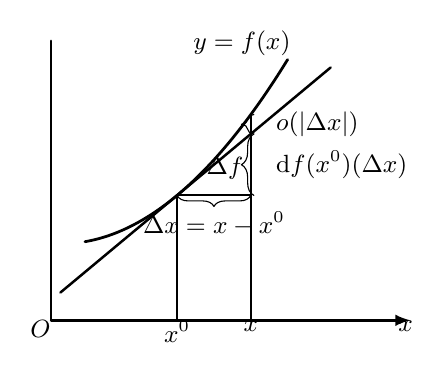
\begin{tikzpicture}[x=0.78cm, y=0.78cm, >=latex, line cap=round, line join=round]
    % ---------- 坐标架 ----------
    \draw[line width=0.9pt] (0, 0) -- (0, 4.55);
    \draw[line width=0.9pt, ->] (0, 0) -- (5.85, 0);
    \node[below left=-1pt, inner sep=1pt] at (0, 0) {\small $O$};
    \node[below left=-1pt, inner sep=1pt] at (5.90, 0) {\small $x$};
    % ---------- 曲线 y = f(x) ----------
    \draw[line width=1.0pt, domain=0.55:3.85, samples=80]
      plot (\x, {1.28 + 0.1727*(\x-0.55) + 0.22*(\x-0.55)*(\x-0.55)});
    \node[anchor=south east, inner sep=1pt] at (3.95, 4.26) {\small $y = f(x)$};
    % ---------- 切线（过 P_0 = (x^0, f(x^0))） ----------
    \draw[line width=0.9pt] (0.15, 0.452) -- (4.55, 4.116);
    % ---------- 竖直/水平辅助线 ----------
    \draw[line width=0.8pt] (2.05, 0) -- (2.05, 2.034);
    \draw[line width=0.8pt] (3.25, 0) -- (3.25, 3.350);
    \draw[line width=0.8pt] (2.05, 2.034) -- (3.25, 2.034);
    \node[below=-1pt, inner sep=1pt] at (2.05, 0) {\small $x^{0}$};
    \node[below=-1pt, inner sep=1pt] at (3.25, 0) {\small $x$};
    % ---------- 大括号与注记 ----------
    \draw[decorate, decoration={brace, amplitude=4pt, mirror}] (2.05, 2.034) -- (3.25, 2.034);
    \node[below=4pt, inner sep=1pt] at (2.65, 2.00) {\small $\Delta x = x - x^{0}$};
    \draw[decorate, decoration={brace, amplitude=4.5pt}] (3.30, 2.034) -- (3.30, 3.033);
    \draw[decorate, decoration={brace, amplitude=4.5pt}] (3.30, 3.033) -- (3.30, 3.350);
    \node[right=6pt, inner sep=1pt] at (3.34, 2.53) {\small $\mathrm{d}f(x^{0})(\Delta x)$};
    \node[right=6pt, inner sep=1pt] at (3.34, 3.19) {\small $o(|\Delta x|)$};
    \node[anchor=east, inner sep=1pt] at (3.18, 2.47) {\small $\Delta f$};
  \end{tikzpicture}
  \caption{}\label{fig:8.2.1}
\end{figure}

\begin{proof}
($\Rightarrow$) 因为 $f$ 在 $x^{0}$ 点可微, 即
\[
  f(x) - f(x^{0}) = A(x - x^{0}) + o(|x - x^{0}|) = A(x - x^{0}) + o(x - x^{0}),
\]
则
\begin{align*}
  \lim_{x \to x^{0}}\frac{f(x) - f(x^{0})}{x - x^{0}}
  &= \lim_{x \to x^{0}}\Big[A + \frac{o(|x - x^{0}|)}{x - x^{0}}\Big] \\
  &= A + 0 = A,
\end{align*}
从而 $f$ 在 $x^{0}$ 点处可导, 且 $f'(x^{0}) = A$.

($\Leftarrow$) 因为 $f$ 在 $x^{0}$ 点可导, 所以
\begin{align*}
  \lim_{x \to x^{0}}\frac{f(x) - f(x^{0}) - f'(x^{0})(x - x^{0})}{x - x^{0}}
  &= \lim_{x \to x^{0}}\Big[\frac{f(x) - f(x^{0})}{x - x^{0}} - f'(x^{0})\Big] \\
  &= f'(x^{0}) - f'(x^{0}) = 0.
\end{align*}
由此得到
\[
  f(x) - f(x^{0}) - f'(x^{0})(x - x^{0}) = o(|x - x^{0}|),
\]
\[
  f(x) - f(x^{0}) = f'(x^{0})(x - x^{0}) + o(|x - x^{0}|).
\]
这就证明了 $f$ 在点 $x^{0}$ 处是可微的.
\end{proof}

\cref{thm:8.2.2}表明, 当 $n = 1$ 时, $f$ 在 $x^{0}$ 可微与可导是彼此等价的. 是否可以指望当 $n \geqslant 2$ 时, $f$ 在 $x^{0}$ 点可微与 $f$ 在 $x^{0}$ 点有偏导数是彼此等价的呢? 下面的定理给出了明确的回答.

\begin{theorem}[可微的必要条件]\label{thm:8.2.3}
$n$ 元函数 $f$ 在 $\boldsymbol{x}^{0}$ 点处可微, 则 $f$ 在 $\boldsymbol{x}^{0}$ 点处有一阶偏导数 $f_{x_{i}}'(\boldsymbol{x}^{0})$, $i = 1, 2, \cdots, n$, 且 $\boldsymbol{A} = \boldsymbol{J}\boldsymbol{f}(\boldsymbol{x}^{0}) = (f_{x_{1}}'(\boldsymbol{x}^{0}), f_{x_{2}}'(\boldsymbol{x}^{0}), \cdots, f_{x_{n}}'(\boldsymbol{x}^{0}))$. 但反之不真.
\end{theorem}

\begin{proof}
设 $n$ 元函数 $f$ 在 $\boldsymbol{x}^{0}$ 点处可微, 令
\[
  x_{j} - x_{j}^{0} = 0, \quad j = 1, 2, \cdots, i - 1, i + 1, \cdots, n,
\]
可以得到
\begin{align*}
  &f(x_{1}^{0}, x_{2}^{0}, \cdots, x_{i-1}^{0}, x_{i}, x_{i+1}^{0}, \cdots, x_{n}^{0}) - f(x_{1}^{0}, x_{2}^{0}, \cdots, x_{i-1}^{0}, x_{i}^{0}, x_{i+1}^{0}, \cdots, x_{n}^{0}) \\
  &= a_{i}(x_{i} - x_{i}^{0}) + o(|x_{i} - x_{i}^{0}|) = a_{i}(x_{i} - x_{i}^{0}) + o(x_{i} - x_{i}^{0}).
\end{align*}
于是,
\begin{align*}
  f_{x_{i}}'(\boldsymbol{x}^{0})
  &= \lim_{x_{i} \to x_{i}^{0}}\frac{f(x_{1}^{0}, x_{2}^{0}, \cdots, x_{i-1}^{0}, x_{i}, x_{i+1}^{0}, \cdots, x_{n}^{0}) - f(x_{1}^{0}, x_{2}^{0}, \cdots, x_{i-1}^{0}, x_{i}^{0}, x_{i+1}^{0}, \cdots, x_{n}^{0})}{x_{i} - x_{i}^{0}} \\
  &= \lim_{x_{i} \to x_{i}^{0}}\frac{a_{i}(x_{i} - x_{i}^{0}) + o(x_{i} - x_{i}^{0})}{x_{i} - x_{i}^{0}} \\
  &= \lim_{x_{i} \to x_{i}^{0}}\Big[a_{i} + \frac{o(x_{i} - x_{i}^{0})}{x_{i} - x_{i}^{0}}\Big] = a_{i} + 0 = a_{i}, \quad i = 1, 2, \cdots, n.
\end{align*}
但反之不真. 例如
\[
  f(x, y) = \begin{cases}
    \dfrac{xy}{x^{2} + y^{2}}, & (x, y) \neq (0, 0), \\[2.5mm]
    0, & (x, y) = (0, 0),
  \end{cases}
\]
易见
\[
  f_{x}'(0, 0) = \lim_{x \to 0}\frac{f(x, 0) - f(0, 0)}{x - 0} = \lim_{x \to 0}0 = 0,
\]
\[
  f_{y}'(0, 0) = \lim_{y \to 0}\frac{f(0, y) - f(0, 0)}{y - 0} = \lim_{y \to 0}0 = 0,
\]
所以
\[
  \boldsymbol{J}f(0, 0) = (f_{x}'(0, 0), f_{y}'(0, 0)) = (0, 0).
\]
\[
  f(x, y) - f(0, 0) = \frac{xy}{x^{2} + y^{2}} - 0 = (0, 0)\binom{x - 0}{y - 0} + \frac{xy}{x^{2} + y^{2}},
\]
现证 $\dfrac{xy}{x^{2} + y^{2}} \neq o(\sqrt{x^{2} + y^{2}})$.

(反证) 假设 $\dfrac{xy}{x^{2} + y^{2}} = o(\sqrt{x^{2} + y^{2}})$, 则
\[
  \lim_{(x, y) \to (0, 0)}\frac{xy}{x^{2} + y^{2}} = \lim_{(x, y) \to (0, 0)}\frac{\dfrac{xy}{x^{2} + y^{2}}}{\sqrt{x^{2} + y^{2}}}\sqrt{x^{2} + y^{2}} = 0 \times 0 = 0.
\]
这与\cref{ex:7.5.5}中二重极限不存在相矛盾. 由上述得到 $f$ 在 $(0, 0)$ 处不可微.

或者从 $\lim_{\substack{x \to 0 \\ y \to 0}}\dfrac{xy}{x^{2} + y^{2}}$ 不存在及\cref{thm:8.2.1}推得 $f$ 在 $(0, 0)$ 处不可微.
\end{proof}

\begin{remark}\label{rem:8.2.1}
因为
\[
  \mathrm{d}f(\boldsymbol{x}^{0})(\Delta\boldsymbol{x}) = \sum_{i=1}^{n}\frac{\partial f}{\partial x_{i}}(\boldsymbol{x}^{0})\Delta x_{i} = \Big(\sum_{i=1}^{n}\frac{\partial f}{\partial x_{i}}(\boldsymbol{x}^{0})\mathrm{d}x_{i}\Big)(\Delta\boldsymbol{x}),
\]
所以
\[
  \mathrm{d}f(\boldsymbol{x}^{0}) = \sum_{i=1}^{n}\frac{\partial f}{\partial x_{i}}(\boldsymbol{x}^{0})\mathrm{d}x_{i},
\]
并称
\[
  \mathrm{d}f = \sum_{i=1}^{n}\frac{\partial f}{\partial x_{i}}\mathrm{d}x_{i}
\]
为 $f$ 的 (全) 微分.
\end{remark}

\begin{theorem}[可微的充分条件]\label{thm:8.2.4}
设 $U \subset \mathbb{R}^{n}$ 为开集, $f: U \to \mathbb{R}^{1}$ 为 $n$ 元函数, 如果 $Jf = (f_{x_{1}}', f_{x_{2}}', \cdots, f_{x_{n}}')$ 在 $\boldsymbol{x}^{0}$ 连续 ($\Leftrightarrow f_{x_{i}}'$ 在 $\boldsymbol{x}^{0}$ 连续, $i = 1, 2, \cdots, n$), 则 $f$ 在 $\boldsymbol{x}^{0}$ 可微. 但反之不真.
\end{theorem}

\begin{proof}
\begin{align*}
  &f(\boldsymbol{x}) - f(\boldsymbol{x}^{0}) \\
  ={} &\sum_{i=1}^{n}\big[f(x_{1}^{0}, x_{2}^{0}, \cdots, x_{i-1}^{0}, x_{i}, x_{i+1}, \cdots, x_{n}) \\
  &\qquad - f(x_{1}^{0}, x_{2}^{0}, \cdots, x_{i-1}^{0}, x_{i}^{0}, x_{i+1}, \cdots, x_{n})\big] \\
  \reasonb{Lagrange 中值定理} {\exists\xi_{i}\ \text{在}\ x_{i}^{0}\ \text{与}\ x_{i}\ \text{之间}}
  ={} &\sum_{i=1}^{n}f_{x_{i}}'(x_{1}^{0}, x_{2}^{0}, \cdots, x_{i-1}^{0}, \xi_{i}, x_{i+1}, \cdots, x_{n})(x_{i} - x_{i}^{0}) \\
  ={} &\sum_{i=1}^{n}f_{x_{i}}'(\boldsymbol{x}^{0})(x_{i} - x_{i}^{0}) + \sum_{i=1}^{n}\alpha_{i}(x_{i} - x_{i}^{0}),
\end{align*}
其中
\begin{align*}
  \alpha_{i} &= f_{x_{i}}'(x_{1}^{0}, x_{2}^{0}, \cdots, x_{i-1}^{0}, \xi_{i}, x_{i+1}, \cdots, x_{n}) - f_{x_{i}}'(x_{1}^{0}, x_{2}^{0}, \cdots, x_{i-1}^{0}, x_{i}^{0}, x_{i+1}^{0}, \cdots, x_{n}^{0}) \\
  &\xrightarrow{Jf\ \text{在}\ \boldsymbol{x}^{0}\ \text{处连续}}\ 0 \quad (\|\boldsymbol{x} - \boldsymbol{x}^{0}\| \to 0). \\
  0 &\leqslant \frac{\big|\sum_{i=1}^{n}\alpha_{i}(x_{i} - x_{i}^{0})\big|}{\|\boldsymbol{x} - \boldsymbol{x}^{0}\|} = \Big|\sum_{i=1}^{n}\alpha_{i}\frac{x_{i} - x_{i}^{0}}{\sqrt{\sum_{j=1}^{n}(x_{j} - x_{j}^{0})^{2}}}\Big| \leqslant \sum_{i=1}^{n}|\alpha_{i}| \to 0 \quad (\|\boldsymbol{x} - \boldsymbol{x}^{0}\| \to 0),
\end{align*}
所以
\[
  \lim_{\boldsymbol{x} \to \boldsymbol{x}^{0}}\frac{\sum_{i=1}^{n}\alpha_{i}(x_{i} - x_{i}^{0})}{\|\boldsymbol{x} - \boldsymbol{x}^{0}\|} = 0,
\]
\[
  f(\boldsymbol{x}) - f(\boldsymbol{x}^{0}) = \sum_{i=1}^{n}f_{x_{i}}'(\boldsymbol{x}^{0})(x_{i} - x_{i}^{0}) + o(\|\boldsymbol{x} - \boldsymbol{x}^{0}\|),
\]
这就证明了 $f$ 在 $\boldsymbol{x}^{0}$ 可微.

但反之不真. 例如: $f: \mathbb{R}^{1} \to \mathbb{R}^{1}$, $x \mapsto f(x)$,
\[
  f(x) = \begin{cases}
    x^{2}\sin\dfrac{1}{x}, & x \neq 0, \\[2.5mm]
    0, & x = 0,
  \end{cases}
\]
\[
  f'(x) = \begin{cases}
    2x\sin\dfrac{1}{x} - \cos\dfrac{1}{x}, & x \neq 0, \\[2.5mm]
    0, & x = 0.
  \end{cases}
\]
根据\cref{thm:8.2.2}, $f$ 在 $0$ 可导 $\Leftrightarrow f$ 在 $0$ 可微. 然而 $f'$ 在 $0$ 不连续.
\end{proof}

可微概念可从 $n$ 元函数继续推广到 Euclid 空间之间的映射.

\begin{definition}\label{def:8.2.2}
设 $U \subset \mathbb{R}^{n}$ 为开集, $f: U \to \mathbb{R}^{m}$ 为映射,
\begin{align*}
  \boldsymbol{x}^{0} &= \begin{pmatrix} x_{1}^{0} \\ \vdots \\ x_{n}^{0} \end{pmatrix} \in U, \quad
  \boldsymbol{x} = \begin{pmatrix} x_{1} \\ \vdots \\ x_{n} \end{pmatrix} \in U, \quad
  \Delta\boldsymbol{x} = \begin{pmatrix} \Delta x_{1} \\ \vdots \\ \Delta x_{n} \end{pmatrix}
  = \begin{pmatrix} x_{1} - x_{1}^{0} \\ \vdots \\ x_{n} - x_{n}^{0} \end{pmatrix} = \boldsymbol{x} - \boldsymbol{x}^{0} \in \mathbb{R}^{n}, \\
  \boldsymbol{f} &= \begin{pmatrix} f_{1} \\ \vdots \\ f_{m} \end{pmatrix}, \quad
  \boldsymbol{A} = \begin{pmatrix} a_{11} & \cdots & a_{1n} \\ \vdots & \ddots & \vdots \\ a_{m1} & \cdots & a_{mn} \end{pmatrix}
\end{align*}
其中 $\boldsymbol{A}$ 为 $m \times n$ 的实矩阵. 如果
\[
  f(\boldsymbol{x}^{0} + \Delta\boldsymbol{x}) - f(\boldsymbol{x}^{0}) = \boldsymbol{A}\Delta\boldsymbol{x} + \boldsymbol{R}(\Delta\boldsymbol{x}), \quad \boldsymbol{R}(\Delta\boldsymbol{x}) = o(\|\Delta\boldsymbol{x}\|), \quad \|\Delta\boldsymbol{x}\| \to 0,
\]
即
\[
  f(\boldsymbol{x}) - f(\boldsymbol{x}^{0}) = \boldsymbol{A}(\boldsymbol{x} - \boldsymbol{x}^{0}) + \boldsymbol{R}(\boldsymbol{x} - \boldsymbol{x}^{0}), \quad \boldsymbol{R}(\boldsymbol{x} - \boldsymbol{x}^{0}) = o(\|\boldsymbol{x} - \boldsymbol{x}^{0}\|), \quad \|\boldsymbol{x} - \boldsymbol{x}^{0}\| \to 0,
\]
则称映射 $f$ 在 $\boldsymbol{x}^{0}$ \textbf{可微}. 记
\[
  \mathrm{d}f(\boldsymbol{x}^{0}): \mathbb{R}^{n} \to \mathbb{R}^{m},
\]
\[
  \mathrm{d}f(\boldsymbol{x}^{0})(\Delta\boldsymbol{x}) = \boldsymbol{A}\Delta\boldsymbol{x},
\]
即
\[
  \mathrm{d}f(\boldsymbol{x}^{0})(\boldsymbol{x} - \boldsymbol{x}^{0}) = \boldsymbol{A}(\boldsymbol{x} - \boldsymbol{x}^{0}).
\]
显然, $\mathrm{d}f(\boldsymbol{x}^{0})$ 为线性映射, 称 $\mathrm{d}f(\boldsymbol{x}^{0})$ 为 $f$ 在点 $\boldsymbol{x}^{0} \in U$ 处的\textbf{微分}.
\end{definition}

考虑分量形式为
\[
  \begin{pmatrix} f_{1}(\boldsymbol{x}^{0} + \Delta\boldsymbol{x}) - f_{1}(\boldsymbol{x}^{0}) \\ \vdots \\ f_{m}(\boldsymbol{x}^{0} + \Delta\boldsymbol{x}) - f_{m}(\boldsymbol{x}^{0}) \end{pmatrix}
  = \begin{pmatrix} a_{11} & \cdots & a_{1n} \\ \vdots & & \vdots \\ a_{m1} & \cdots & a_{mn} \end{pmatrix}
    \begin{pmatrix} \Delta x_{1} \\ \vdots \\ \Delta x_{n} \end{pmatrix}
  + \begin{pmatrix} R_{1}(\Delta\boldsymbol{x}) \\ \vdots \\ R_{m}(\Delta\boldsymbol{x}) \end{pmatrix}
\]
\[
  \Leftrightarrow f_{i}(\boldsymbol{x}^{0} + \Delta\boldsymbol{x}) - f_{i}(\boldsymbol{x}^{0}) = (a_{i1}, a_{i2}, \cdots, a_{in})\begin{pmatrix} \Delta x_{1} \\ \vdots \\ \Delta x_{n} \end{pmatrix} + R_{i}(\Delta\boldsymbol{x}),
\]
\[
  R_{i}(\Delta\boldsymbol{x}) = o(\|\Delta\boldsymbol{x}\|), \quad \|\Delta\boldsymbol{x}\| \to 0, \quad i = 1, 2, \cdots, m.
\]
$\Leftrightarrow f_{i}$ 在 $\boldsymbol{x}^{0}$ 是可微的, $i = 1, 2, \cdots, m$.

读者可用另一形式 (即 $\boldsymbol{x}$, $\boldsymbol{x} - \boldsymbol{x}^{0}$) 表达上述式子.

由上述讨论立即有下面定理.

\begin{theorem}\label{thm:8.2.5}
设 $U \subset \mathbb{R}^{n}$ 为开集, 映射 $f: U \to \mathbb{R}^{m}$ 在 $\boldsymbol{x}^{0} \in U$ 可微 $\Leftrightarrow n$ 元函数 $f_{i}\ (i = 1, 2, \cdots, m)$ 在 $\boldsymbol{x}^{0}$ 点可微.
\end{theorem}

类似 $n$ 元函数的\cref{thm:8.2.1}, \cref{thm:8.2.3}, \cref{thm:8.2.4}, 关于映射也有以下相应的定理.

\setcounter{theorem}{1}
\begin{theoremp}\label{thm:8.2.1p}
设 $U \subset \mathbb{R}^{n}$ 为开集, 映射 $f: U \to \mathbb{R}^{m}$ 在 $\boldsymbol{x}^{0}$ 处可微, 必有 $f$ 在 $\boldsymbol{x}^{0}$ 处连续. 但反之不真.
\end{theoremp}

\begin{proof}
类似\cref{thm:8.2.1}的证明.
\end{proof}

\setcounter{theorem}{3}
\begin{theoremp}[可微的必要条件]\label{thm:8.2.3p}
设 $U \subset \mathbb{R}^{n}$ 为开集, $f: U \to \mathbb{R}^{n}$ 为映射, 且 $f$ 在 $\boldsymbol{x}^{0}$ 点处可微, 则 $\dfrac{\partial f_{i}}{\partial x_{j}}(\boldsymbol{x}^{0})$ 存在有限, 且
\[
  \boldsymbol{A} = \Big(\frac{\partial f_{i}}{\partial x_{j}}\Big)\Big|_{\boldsymbol{x}^{0}} = \begin{pmatrix}
    \dfrac{\partial f_{1}}{\partial x_{1}} & \cdots & \dfrac{\partial f_{1}}{\partial x_{n}} \\[2mm]
    \vdots & & \vdots \\[1mm]
    \dfrac{\partial f_{m}}{\partial x_{1}} & \cdots & \dfrac{\partial f_{m}}{\partial x_{n}}
  \end{pmatrix}_{\boldsymbol{x}^{0}} = \boldsymbol{J}\boldsymbol{f}(\boldsymbol{x}^{0}) = \mathrm{grad}\,f\Big|_{\boldsymbol{x}^{0}},
\]
并称 $\mathrm{grad}\,f\big|_{\boldsymbol{x}^{0}} = Jf(\boldsymbol{x}^{0})$ 为 $f$ 在 $\boldsymbol{x}^{0}$ 处的 Jacobi 矩阵, 或 $f$ 在 $\boldsymbol{x}^{0}$ 的``导数'', 或 $f$ 的\textbf{梯度} (gradient). 但反之不真.
\end{theoremp}

\begin{proof}
$f$ 在 $\boldsymbol{x}^{0}$ 处可微 $\Leftrightarrow f_{i}$ 在 $\boldsymbol{x}^{0}$ 处可微, $i = 1, 2, \cdots, m$, 由\cref{thm:8.2.3}可知, $\dfrac{\partial f_{i}}{\partial x_{j}}(\boldsymbol{x}^{0})$ 存在有限, $i = 1, 2, \cdots, m$; $j = 1, 2, \cdots, n$.

但反之不真. 反例见\cref{thm:8.2.3}中的反例.
\end{proof}

如果 $f$ 在任何 $\boldsymbol{x} \in U \subset \mathbb{R}^{n}$ 有偏导数, 则
\[
  Jf: U \to \mathbb{R}^{mn},
\]
\[
  \boldsymbol{x} \mapsto \boldsymbol{J}\boldsymbol{f}(\boldsymbol{x}) = \begin{pmatrix}
    \dfrac{\partial f_{1}}{\partial x_{1}} & \cdots & \dfrac{\partial f_{1}}{\partial x_{n}} \\[2mm]
    \vdots & & \vdots \\[1mm]
    \dfrac{\partial f_{m}}{\partial x_{1}} & \cdots & \dfrac{\partial f_{m}}{\partial x_{n}}
  \end{pmatrix}_{\boldsymbol{x}}
\]
为一映射. 于是
\[
  \mathrm{d}f(\boldsymbol{x}^{0})(\Delta\boldsymbol{x}) = Jf(\boldsymbol{x}^{0})\Delta\boldsymbol{x}.
\]
令
\[
  \mathrm{d}x_{i}(\Delta x_{j}) = \delta_{ij} = \begin{cases}
    1, & i \neq j, \\
    0, & i = j,
  \end{cases}
\]
则
\[
  \mathrm{d}f_{i}\Big|_{\boldsymbol{x}^{0}} = \sum_{j=1}^{n}\frac{\partial f_{i}}{\partial x_{j}}(\boldsymbol{x}^{0})\mathrm{d}x_{j},
\]
\[
  \mathrm{d}\boldsymbol{f}\Big|_{\boldsymbol{x}^{0}} = \begin{pmatrix} \mathrm{d}f_{1} \\ \vdots \\ \mathrm{d}f_{m} \end{pmatrix}\Big|_{\boldsymbol{x}^{0}} = \begin{pmatrix}
    \displaystyle\sum_{j=1}^{n}\frac{\partial f_{1}}{\partial x_{j}}(\boldsymbol{x}^{0})\mathrm{d}x_{j} \\ \vdots \\
    \displaystyle\sum_{j=1}^{n}\frac{\partial f_{m}}{\partial x_{j}}(\boldsymbol{x}^{0})\mathrm{d}x_{j}
  \end{pmatrix}
\]
\[
  = \begin{pmatrix}
    \displaystyle\frac{\partial f_{1}}{\partial x_{1}} & \cdots & \displaystyle\frac{\partial f_{1}}{\partial x_{n}} \\[3mm]
    \vdots & & \vdots \\[2mm]
    \displaystyle\frac{\partial f_{m}}{\partial x_{1}} & \cdots & \displaystyle\frac{\partial f_{m}}{\partial x_{n}}
  \end{pmatrix}_{\boldsymbol{x}^{0}} \begin{pmatrix} \mathrm{d}x_{1} \\ \vdots \\ \mathrm{d}x_{n} \end{pmatrix} = \boldsymbol{J}\boldsymbol{f}(\boldsymbol{x}^{0})\mathrm{d}\boldsymbol{x},
\]
并称它为映射 $f$ 的 (全) 微分.

\setcounter{theorem}{4}
\begin{theoremp}[可微的充分条件]\label{thm:8.2.4p}
设 $U \subset \mathbb{R}^{n}$ 为开集, $f: U \to \mathbb{R}^{m}$ 为映射, 如果 $f$ 的 Jacobi 矩阵 $Jf = \Big(\dfrac{\partial f_{i}}{\partial x_{j}}\Big)$ 在 $\boldsymbol{x}^{0}$ 连续, 则 $f$ 在 $\boldsymbol{x}^{0}$ 可微. 但反之不真.
\end{theoremp}

\begin{proof}
\begin{align*}
  Jf = \Big(\frac{\partial f_{i}}{\partial x_{j}}\Big)\ \text{在}\ \boldsymbol{x}^{0}\ \text{连续}
  &\Leftrightarrow Jf_{i}\ \text{在}\ \boldsymbol{x}^{0}\ \text{连续},\ i = 1, 2, \cdots, m \\
  &\overset{\text{定理}\ 8.2.4}{\Longleftrightarrow} f_{i}\ \text{在}\ \boldsymbol{x}^{0}\ \text{可微},\ i = 1, 2, \cdots, m \\
  &\overset{\text{定理}\ 8.2.5}{\Longleftrightarrow} f\ \text{在}\ \boldsymbol{x}^{0}\ \text{可微}. \qedhere
\end{align*}
\end{proof}

\setcounter{theorem}{5}
\begin{remark}\label{rem:8.2.2}
从\cref{thm:8.2.3p}与\cref{thm:8.2.4p}可知, $f$ 的一阶偏导数 $\dfrac{\partial f_{i}}{\partial x_{j}}$ 在 $\boldsymbol{x}^{0}$ 连续 $\Rightarrow f$ 在 $\boldsymbol{x}^{0}$ 可微 $\Rightarrow f$ 在 $\boldsymbol{x}^{0}$ 有一阶偏导数 $\dfrac{\partial f_{i}}{\partial x_{j}}$, $i = 1, 2, \cdots, m$; $j = 1, 2, \cdots, n$. 因此, 可微是介于 $f$ 的一阶偏导数在 $\boldsymbol{x}^{0}$ 连续与 $f$ 在 $\boldsymbol{x}^{0}$ 有一阶偏导数之间的一个概念.
\end{remark}

\begin{definition}\label{def:8.2.3}
设 $U \subset \mathbb{R}^{n}$ 为开集, $f: U \to \mathbb{R}^{m}$ 为 $C^{k}$ 映射:

$k = 0$, $f$ 为连续映射;

$0 < k < +\infty$, $f_{i}$ 有直到 $k$ 阶连续偏导数, $i = 1, 2, \cdots, m$;

$k = +\infty$, $f_{i}$ 具有各阶连续偏导数, $i = 1, 2, \cdots, m$;

$k = \omega$, $f_{i}$ 实解析, 即在 $U$ 中任一点 $\boldsymbol{x}^{0} = (x_{1}^{0}, x_{2}^{0}, \cdots, x_{n}^{0})$ 的邻近可展开为收敛的 ($n$ 元) 幂级数, $i = 1, 2, \cdots, m$.

记 $C^{k}(U, \mathbb{R}^{m})$ 为从 $U$ 到 $\mathbb{R}^{m}$ 的 $C^{k}$ 映射的全体.
\end{definition}

将\cref{thm:8.1.3}推广为映射的复合求导链规则有下面的定理.

\begin{theorem}[映射的复合求导的链规则]\label{thm:8.2.6}
设 $U \subset \mathbb{R}^{l}$ 与 $V \subset \mathbb{R}^{n}$ 都为开集,
\[
  \boldsymbol{g}: U \to V \quad \text{与} \quad f: V \to \mathbb{R}^{m}
\]
都为映射, $\boldsymbol{g}$ 在 $\boldsymbol{u}^{0} \in U$ 可微, $f$ 在 $\boldsymbol{x}^{0} = \boldsymbol{g}(\boldsymbol{u}^{0})$ 可微, 则复合映射 $f \circ \boldsymbol{g}$ 在 $\boldsymbol{u}^{0}$ 也可微, 且
\[
  \boldsymbol{J}(f \circ \boldsymbol{g})'(\boldsymbol{u}^{0}) = \boldsymbol{J}f(\boldsymbol{x}^{0})\boldsymbol{J}\boldsymbol{g}(\boldsymbol{u}^{0}).
\]
\end{theorem}

\begin{proof}
$\boldsymbol{g}$ 在 $\boldsymbol{u}^{0}$ 可微, 即
\[
  \boldsymbol{g}(\boldsymbol{u}) - \boldsymbol{g}(\boldsymbol{u}^{0}) = \boldsymbol{J}\boldsymbol{g}(\boldsymbol{u}^{0})(\boldsymbol{u} - \boldsymbol{u}^{0}) + \boldsymbol{R}_{g}(\boldsymbol{u} - \boldsymbol{u}^{0}),
\]
\[
  \boldsymbol{R}_{g}(\boldsymbol{u} - \boldsymbol{u}^{0}) = o(\boldsymbol{u} - \boldsymbol{u}^{0}), \quad \boldsymbol{u} \to \boldsymbol{u}^{0}.
\]
又 $f$ 在 $\boldsymbol{x}^{0} = \boldsymbol{g}(\boldsymbol{u}^{0})$ 可微, 故
\[
  f(\boldsymbol{x}) - f(\boldsymbol{x}^{0}) = Jf(\boldsymbol{x}^{0})(\boldsymbol{x} - \boldsymbol{x}^{0}) + R_{f}(\boldsymbol{x} - \boldsymbol{x}^{0}),
\]
\[
  \boldsymbol{R}_{f}(\boldsymbol{x} - \boldsymbol{x}^{0}) = o(\boldsymbol{x} - \boldsymbol{x}^{0}), \quad \boldsymbol{x} \to \boldsymbol{x}^{0}.
\]
令 $\boldsymbol{x} = \boldsymbol{g}(\boldsymbol{u})$, $\boldsymbol{x}^{0} = \boldsymbol{g}(\boldsymbol{u}^{0})$ 代入上式得到
\begin{align*}
  f \circ \boldsymbol{g}(\boldsymbol{u}) - f \circ \boldsymbol{g}(\boldsymbol{u}^{0})
  &= \boldsymbol{J}f(\boldsymbol{x}^{0})(\boldsymbol{g}(\boldsymbol{u}) - \boldsymbol{g}(\boldsymbol{u}^{0})) + \boldsymbol{R}_{f}(\boldsymbol{g}(\boldsymbol{u}) - \boldsymbol{g}(\boldsymbol{u}^{0})) \\
  &= \boldsymbol{J}f(\boldsymbol{x}^{0})\big[\boldsymbol{J}\boldsymbol{g}(\boldsymbol{u}^{0})(\boldsymbol{u} - \boldsymbol{u}^{0}) + \boldsymbol{R}_{g}(\boldsymbol{u} - \boldsymbol{u}^{0})\big] + \boldsymbol{R}_{f}(\boldsymbol{g}(\boldsymbol{u}) - \boldsymbol{g}(\boldsymbol{u}^{0})) \\
  &= \boldsymbol{J}f(\boldsymbol{x}^{0})\boldsymbol{J}\boldsymbol{g}(\boldsymbol{u}^{0})(\boldsymbol{u} - \boldsymbol{u}^{0}) + \boldsymbol{R}_{f \circ g}(\boldsymbol{u} - \boldsymbol{u}^{0}),
\end{align*}
其中
\[
  \|\boldsymbol{J}f(\boldsymbol{x}^{0})\boldsymbol{R}_{g}(\boldsymbol{u} - \boldsymbol{u}^{0})\| \overset{\text{8.2 练习题 26}}{\leqslant} \|\boldsymbol{J}f(\boldsymbol{x}^{0})\|\|\boldsymbol{R}_{g}(\boldsymbol{u} - \boldsymbol{u}^{0})\| = o(\boldsymbol{u} - \boldsymbol{u}^{0}),
\]
\[
  \text{矩阵}\ \boldsymbol{A}\ \text{的模}\quad \|\boldsymbol{A}\| = \sqrt{\sum_{i=1}^{m}\sum_{j=1}^{n}a_{ij}^{2}}.
\]
\begin{align*}
  0 \leqslant {}& \frac{\|\boldsymbol{R}_{f}(\boldsymbol{g}(\boldsymbol{u}) - \boldsymbol{g}(\boldsymbol{u}^{0}))\|}{\|\boldsymbol{u} - \boldsymbol{u}^{0}\|} \\
  = {}& \frac{\|\boldsymbol{R}_{f}(\boldsymbol{g}(\boldsymbol{u}) - \boldsymbol{g}(\boldsymbol{u}^{0}))\|}{\|\boldsymbol{g}(\boldsymbol{u}) - \boldsymbol{g}(\boldsymbol{u}^{0})\|} \cdot \frac{\|\boldsymbol{g}(\boldsymbol{u}) - \boldsymbol{g}(\boldsymbol{u}^{0})\|}{\|\boldsymbol{u} - \boldsymbol{u}^{0}\|} \\
  \leqslant {}& \frac{\|\boldsymbol{R}_{f}(\boldsymbol{g}(\boldsymbol{u}) - \boldsymbol{g}(\boldsymbol{u}^{0}))\|}{\|\boldsymbol{g}(\boldsymbol{u}) - \boldsymbol{g}(\boldsymbol{u}^{0})\|}\Big[\|\boldsymbol{J}\boldsymbol{g}(\boldsymbol{u}^{0})\| + \frac{\|\boldsymbol{R}_{g}(\boldsymbol{u} - \boldsymbol{u}^{0})\|}{\boldsymbol{u} - \boldsymbol{u}^{0}}\Big] \\
  \to {}& 0 \quad (\boldsymbol{u} \to \boldsymbol{u}^{0},\ \text{由}\ \boldsymbol{g}\ \text{连续知},\ \boldsymbol{g}(\boldsymbol{u}) \to \boldsymbol{g}(\boldsymbol{u}^{0}));
\end{align*}
注意, 当 $\boldsymbol{g}(\boldsymbol{u}) = \boldsymbol{g}(\boldsymbol{u}^{0})$ 时, 上式也有
\[
  \frac{\|\boldsymbol{R}_{f}(\boldsymbol{g}(\boldsymbol{u}) - \boldsymbol{g}(\boldsymbol{u}^{0}))\|}{\|\boldsymbol{u} - \boldsymbol{u}^{0}\|} = \frac{\|\boldsymbol{R}_{f}(\boldsymbol{0})\|}{\|\boldsymbol{u} - \boldsymbol{u}^{0}\|} = 0 \to 0 \quad (\boldsymbol{u} \to \boldsymbol{u}^{0}).
\]
因此 $f \circ \boldsymbol{g}$ 在 $\boldsymbol{u}^{0}$ 可微, 且
\[
  \boldsymbol{J}(f \circ \boldsymbol{g})(\boldsymbol{u}^{0}) = \boldsymbol{J}f(\boldsymbol{x}^{0})\boldsymbol{J}\boldsymbol{g}(\boldsymbol{u}^{0}).
\]
\end{proof}

\begin{remark}\label{rem:8.2.3}
\[
  \boldsymbol{y} = f(\boldsymbol{x}), \quad \boldsymbol{x} = \boldsymbol{g}(\boldsymbol{u}),
\]
\[
  \boldsymbol{J}(f \circ \boldsymbol{g})(\boldsymbol{u}^{0}) = \boldsymbol{J}f(\boldsymbol{x}^{0})\boldsymbol{J}\boldsymbol{g}(\boldsymbol{u}^{0}),
\]
其分量形式表达为
\[
  \begin{pmatrix} y_{1} \\ \vdots \\ y_{m} \end{pmatrix} = \begin{pmatrix} f_{1}(x_{1}, \cdots, x_{n}) \\ \vdots \\ f_{m}(x_{1}, \cdots, x_{n}) \end{pmatrix}, \quad
  \begin{pmatrix} x_{1} \\ \vdots \\ x_{n} \end{pmatrix} = \begin{pmatrix} g_{1}(u_{1}, \cdots, u_{l}) \\ \vdots \\ g_{n}(u_{1}, \cdots, u_{l}) \end{pmatrix},
\]
\[
  \begin{pmatrix}
    \displaystyle\frac{\partial y_{1}}{\partial u_{1}} & \cdots & \displaystyle\frac{\partial y_{1}}{\partial u_{l}} \\[3mm]
    \vdots & & \vdots \\[2mm]
    \displaystyle\frac{\partial y_{m}}{\partial u_{1}} & \cdots & \displaystyle\frac{\partial y_{m}}{\partial u_{l}}
  \end{pmatrix} = \begin{pmatrix}
    \displaystyle\frac{\partial y_{1}}{\partial x_{1}} & \cdots & \displaystyle\frac{\partial y_{1}}{\partial x_{n}} \\[3mm]
    \vdots & & \vdots \\[2mm]
    \displaystyle\frac{\partial y_{m}}{\partial x_{1}} & \cdots & \displaystyle\frac{\partial y_{m}}{\partial x_{n}}
  \end{pmatrix}\begin{pmatrix}
    \displaystyle\frac{\partial x_{1}}{\partial u_{1}} & \cdots & \displaystyle\frac{\partial x_{1}}{\partial u_{l}} \\[3mm]
    \vdots & & \vdots \\[2mm]
    \displaystyle\frac{\partial x_{n}}{\partial u_{1}} & \cdots & \displaystyle\frac{\partial x_{n}}{\partial u_{l}}
  \end{pmatrix},
\]
即
\[
  \frac{\partial y_{i}}{\partial u_{j}} = \sum_{k=1}^{n}\frac{\partial y_{i}}{\partial x_{k}}\frac{\partial x_{k}}{\partial u_{j}}, \quad i = 1, 2, \cdots, m; \quad j = 1, 2, \cdots, l.
\]
\end{remark}

这就是多变量函数求导的链规则公式. 最后一式适合于单个分量 $y_{i}$ 的求导, 因为它不涉及到其他分量 $y_{j}$ 的求导, 所以不必大张旗鼓地应用上述矩阵公式来计算.

应该指出, 上述矩阵公式特别适用于全部分量 $y_{i}$ 的偏导数计算与整体性论证的简捷表达.

可微定义可以换成下面的等价形式, 它在使用时比较方便.

\begin{theorem}\label{thm:8.2.7}
设 $U \subset \mathbb{R}^{n}$ 为开集, 则

映射 $f: U \to \mathbb{R}^{m}$ 在点 $\boldsymbol{x}^{0}$ 处可微 $\Leftrightarrow$
\[
  f(\boldsymbol{x}^{0} + \Delta\boldsymbol{x}) - f(\boldsymbol{x}^{0}) = Jf(\boldsymbol{x}^{0})\Delta\boldsymbol{x} + B(\Delta\boldsymbol{x})\Delta\boldsymbol{x},
\]
其中 $B(\Delta\boldsymbol{x})$ 为 $m \times n$ 矩阵, 且
\[
  \lim_{\Delta\boldsymbol{x} \to \boldsymbol{0}}\boldsymbol{B}(\Delta\boldsymbol{x}) = \boldsymbol{0}.
\]
\end{theorem}

\begin{proof}
($\Leftarrow$) 显然有
\[
  0 \leqslant \frac{1}{\|\Delta\boldsymbol{x}\|}\|\boldsymbol{B}(\Delta\boldsymbol{x})\Delta\boldsymbol{x}\| = \Big\|\boldsymbol{B}(\Delta\boldsymbol{x})\frac{\Delta\boldsymbol{x}}{\|\Delta\boldsymbol{x}\|}\Big\|
\]
\[
  \overset{\text{8.2 练习题 26}}{\leqslant} \|\boldsymbol{B}(\Delta\boldsymbol{x})\|\Big\|\frac{\Delta\boldsymbol{x}}{\|\Delta\boldsymbol{x}\|}\Big\| = \|\boldsymbol{B}(\Delta\boldsymbol{x})\| \to 0 \quad (\|\Delta\boldsymbol{x}\| \to 0).
\]
因此,
\[
  \boldsymbol{B}(\Delta\boldsymbol{x})\Delta\boldsymbol{x} = o(\|\Delta\boldsymbol{x}\|).
\]
根据\cref{def:8.2.2}, $f$ 在点 $\boldsymbol{x}^{0}$ 处可微.

($\Rightarrow$) 设 $f$ 在点 $\boldsymbol{x}^{0}$ 处可微, 则
\[
  \boldsymbol{R}_{f}(\Delta\boldsymbol{x}) = \boldsymbol{f}(\boldsymbol{x}^{0} + \Delta\boldsymbol{x}) - \boldsymbol{f}(\boldsymbol{x}^{0}) - \boldsymbol{J}\boldsymbol{f}(\boldsymbol{x}^{0})\Delta\boldsymbol{x},
\]
\[
  \boldsymbol{R}_{f}(\Delta\boldsymbol{x}) = o(\|\Delta\boldsymbol{x}\|) \quad (\|\Delta\boldsymbol{x}\| \to 0).
\]
令
\[
  \boldsymbol{B}(\Delta\boldsymbol{x}) = \begin{cases}
    \dfrac{\boldsymbol{R}_{f}(\Delta\boldsymbol{x})}{\|\Delta\boldsymbol{x}\|}\dfrac{\Delta\boldsymbol{x}}{\|\Delta\boldsymbol{x}\|}, & \Delta\boldsymbol{x} \neq \boldsymbol{0}, \\[3mm]
    \boldsymbol{0}, & \Delta\boldsymbol{x} = \boldsymbol{0}.
  \end{cases}
\]
由于
\[
  0 \leqslant \|\boldsymbol{B}(\Delta\boldsymbol{x})\| = \Big\|\frac{\boldsymbol{R}_{f}(\Delta\boldsymbol{x})}{\|\Delta\boldsymbol{x}\|}\frac{\Delta\boldsymbol{x}}{\|\Delta\boldsymbol{x}\|}\Big\| = \Big\|\frac{\boldsymbol{R}_{f}(\Delta\boldsymbol{x})}{\|\Delta\boldsymbol{x}\|}\Big\| \to 0 \quad (\|\Delta\boldsymbol{x}\| \to 0),
\]
就有
\[
  \lim_{\|\Delta\boldsymbol{x}\| \to 0}\boldsymbol{B}(\Delta\boldsymbol{x}) = \boldsymbol{0}.
\]
而
\[
  \boldsymbol{B}(\Delta\boldsymbol{x})\Delta\boldsymbol{x} = \begin{cases}
    \dfrac{\boldsymbol{R}_{f}(\Delta\boldsymbol{x})}{\|\Delta\boldsymbol{x}\|}\dfrac{\Delta\boldsymbol{x}}{\|\Delta\boldsymbol{x}\|}\Delta\boldsymbol{x}, & \Delta\boldsymbol{x} \neq \boldsymbol{0}, \\[3mm]
    \boldsymbol{0}, & \Delta\boldsymbol{x} = \boldsymbol{0},
  \end{cases}
\]
\[
  \boldsymbol{B}(\Delta\boldsymbol{x})\Delta\boldsymbol{x} = \boldsymbol{R}_{f}(\Delta\boldsymbol{x}) = \boldsymbol{f}(\boldsymbol{x}^{0} + \Delta\boldsymbol{x}) - \boldsymbol{f}(\boldsymbol{x}^{0}) - \boldsymbol{J}\boldsymbol{f}(\boldsymbol{x}^{0})\Delta\boldsymbol{x},
\]
即
\[
  f(\boldsymbol{x}^{0} + \Delta\boldsymbol{x}) - f(\boldsymbol{x}^{0}) = Jf(\boldsymbol{x}^{0})\Delta\boldsymbol{x} + \boldsymbol{B}(\Delta\boldsymbol{x})\Delta\boldsymbol{x}. \qedhere
\]
\end{proof}

在一元函数微分学中, Lagrange 中值定理起着很重要的作用. 应用这个定理, 证明了开区间内导数为零的函数 $f$ 必为常值函数; 应用这个定理, 可以通过函数导数的正负来判断这个函数的增减性. 在讨论高维 Euclid 空间之间的映射时, 有与一元函数的导数相对应的概念, 它就是该映射的 Jacobi 矩阵. 至此, 自然会问: 有没有类似于 Lagrange 中值定理的定理? 对于定义在凸区域上的可微函数, 中值定理是正确的.

\begin{theorem}[高维微分中值定理]\label{thm:8.2.8}
设 $U \subset \mathbb{R}^{n}$ 为凸区域, 函数 $f: U \to \mathbb{R}^{1}$ 可微, 则 $\forall \boldsymbol{a}, \boldsymbol{b} \in U$, 在 $\boldsymbol{a}$ 与 $\boldsymbol{b}$ 的连线内部必有一点 $\boldsymbol{\xi}$, 使得
\[
  f(\boldsymbol{b}) - f(\boldsymbol{a}) = \boldsymbol{J}f(\boldsymbol{\xi})(\boldsymbol{b} - \boldsymbol{a}).
\]
\end{theorem}

\begin{proof}
显然, $\boldsymbol{a}$ 与 $\boldsymbol{b}$ 连线上的点可表示为 $(1 - t)\boldsymbol{a} + t\boldsymbol{b}$, $t \in [0, 1]$. 令
\[
  \varphi(t) = f((1 - t)\boldsymbol{a} + t\boldsymbol{b}), \quad t \in [0, 1],
\]
它是一个可微函数, 由\cref{thm:8.2.2}知, $\varphi$ 在 $[0, 1]$ 上为可导函数. 根据一元函数的 Lagrange 中值定理, $\exists\theta \in (0, 1)$, s.t.
\[
  \varphi(1) - \varphi(0) = \varphi'(\theta)(1 - 0) = \varphi'(\theta),
\]
即
\begin{align*}
  f(\boldsymbol{b}) - f(\boldsymbol{a}) &= \sum_{i=1}^{n}f_{x_{i}}'((1 - \theta)\boldsymbol{a} + \theta\boldsymbol{b})(b_{i} - a_{i}) \\
  &= \boldsymbol{J}\boldsymbol{f}(\boldsymbol{\xi})(\boldsymbol{b} - \boldsymbol{a}),
\end{align*}
其中 $\boldsymbol{\xi} = (1 - \theta)\boldsymbol{a} + \theta\boldsymbol{b}$.
\end{proof}

关于映射, 我们有拟微分中值定理. 为此, 先证下面特殊情形的\cref{lem:8.2.1}.

\begin{lemma}\label{lem:8.2.1}
设映射 $f: [a, b] \to \mathbb{R}^{m}$ 连续, 在 $(a, b)$ 内可微, 则 $\exists\xi \in (a, b)$, s.t.
\[
  \|f(b) - f(a)\| \leqslant \|Jf(\xi)\|(b - a).
\]
\end{lemma}

\begin{proof}
令 $\varphi(t) = \langle\boldsymbol{f}(b) - \boldsymbol{f}(a), \boldsymbol{f}(t)\rangle$. 显然, $\varphi$ 在 $[a, b]$ 上连续, 在 $(a, b)$ 内可微, 根据\cref{thm:8.2.2}, $\varphi$ 在 $(a, b)$ 内可导. 对 $\varphi$ 应用 Lagrange 中值定理, $\exists\xi \in (a, b)$, s.t.
\[
  \varphi(b) - \varphi(a) = (b - a)\varphi'(\xi) = (b - a)\langle f(b) - f(a), \boldsymbol{J}f(\xi)\rangle.
\]
另一方面,
\begin{align*}
  \varphi(b) - \varphi(a) &= \langle\boldsymbol{f}(b) - \boldsymbol{f}(a), \boldsymbol{f}(b)\rangle - \langle\boldsymbol{f}(b) - \boldsymbol{f}(a), \boldsymbol{f}(a)\rangle \\
  &= \langle\boldsymbol{f}(b) - \boldsymbol{f}(a), \boldsymbol{f}(b) - \boldsymbol{f}(a)\rangle = \|\boldsymbol{f}(b) - \boldsymbol{f}(a)\|^{2}.
\end{align*}
根据 Cauchy-Schwarz 不等式有
\begin{align*}
  \|\boldsymbol{f}(b) - \boldsymbol{f}(a)\|^{2} &= (b - a)\langle\boldsymbol{f}(b) - \boldsymbol{f}(a), \boldsymbol{J}\boldsymbol{f}(\xi)\rangle \\
  &\leqslant (b - a)\|\boldsymbol{f}(b) - \boldsymbol{f}(a)\|\|\boldsymbol{J}\boldsymbol{f}(\xi)\|,
\end{align*}
当 $f(b) - f(a) \neq 0$ 时, 两边消去 $\|\boldsymbol{f}(b) - \boldsymbol{f}(a)\|$ 得到
\[
  \|\boldsymbol{f}(b) - \boldsymbol{f}(a)\| \leqslant (b - a)\|\boldsymbol{J}\boldsymbol{f}(\xi)\|.
\]
注意, 当 $f(b) - f(a) = 0$ 时, 上式自然成立 (可以任取 $\xi \in (a, b)$).
\end{proof}

应用\cref{lem:8.2.1}立即推得映射的拟微分中值定理.

\begin{theorem}[映射的拟微分中值定理]\label{thm:8.2.9}
设 $U \subset \mathbb{R}^{n}$ 为凸区域, 映射 $f: U \to \mathbb{R}^{m}$ 在 $U$ 上连续, 在 $U^{\circ}$ 内可微, 则 $\forall \boldsymbol{a}, \boldsymbol{b} \in U$, 在由 $\boldsymbol{a}$ 与 $\boldsymbol{b}$ 所决定的线段内必有一点 $\boldsymbol{\xi}$, s.t.
\[
  \|f(\boldsymbol{b}) - f(\boldsymbol{a})\| \leqslant \|Jf(\boldsymbol{\xi})\|\|\boldsymbol{b} - \boldsymbol{a}\|.
\]
\end{theorem}

\begin{proof}
由 $\boldsymbol{a}$ 与 $\boldsymbol{b}$ 所决定的线段可表示成
\[
  \boldsymbol{r}(t) = (1 - t)\boldsymbol{a} + t\boldsymbol{b}, \quad t \in [0, 1].
\]
令
\[
  \boldsymbol{g}(t) = \boldsymbol{f} \circ \boldsymbol{r}(t) = \boldsymbol{f}(\boldsymbol{r}(t)), \quad t \in [0, 1].
\]
$\boldsymbol{g}$ 在 $[0, 1]$ 上连续, 在 $(0, 1)$ 内可微, 根据\cref{thm:8.2.2}, $\boldsymbol{g}$ 在 $(0, 1)$ 内可导. 再由复合映射求导的链规则可得
\[
  \boldsymbol{J}\boldsymbol{g}(t) = \boldsymbol{J}\boldsymbol{f}(\boldsymbol{r}(t))\boldsymbol{J}\boldsymbol{r}(t) = \boldsymbol{J}\boldsymbol{f}(\boldsymbol{r}(t))(\boldsymbol{b} - \boldsymbol{a}).
\]
应用\cref{lem:8.2.1}, 有
\[
  \|\boldsymbol{g}(1) - \boldsymbol{g}(0)\| \leqslant \|\boldsymbol{J}\boldsymbol{g}(\theta)\|(1 - 0) = \|\boldsymbol{J}\boldsymbol{g}(\theta)\|, \quad \theta \in (0, 1).
\]
若令 $\boldsymbol{\xi} = \boldsymbol{r}(\theta) = (1 - \theta)\boldsymbol{a} + \theta\boldsymbol{b}$, 它是由 $\boldsymbol{a}$ 与 $\boldsymbol{b}$ 所决定的线段内的一点, 则有
\begin{align*}
  \|f(\boldsymbol{b}) - f(\boldsymbol{a})\| &= \|\boldsymbol{g}(1) - \boldsymbol{g}(0)\| \leqslant \|\boldsymbol{J}\boldsymbol{g}(\theta)\| \\
  &= \|\boldsymbol{J}f(r(\theta))(\boldsymbol{b} - \boldsymbol{a})\| \leqslant \|\boldsymbol{J}f(\boldsymbol{\xi})\|\|\boldsymbol{b} - \boldsymbol{a}\|.
\end{align*}
\end{proof}

作为拟微分中值定理的应用, 我们来推广\cref{thm:8.1.6}.

\begin{theorem}\label{thm:8.2.10}
设 $U \subset \mathbb{R}^{n}$ 为开区域, 映射 $f: \overline{U} \to \mathbb{R}^{m}$ 连续, 在 $U$ 上可微, 且 $Jf = 0$, 则 $f$ 在 $\overline{U}$ 上为一常向量.
\end{theorem}

\begin{proof}[证法 1]
如果 $V \subset U$ 为一凸区域, 由\cref{thm:8.2.9}, 对 $\forall \boldsymbol{a}, \boldsymbol{b} \in V$, 有
\begin{align*}
  0 \leqslant \|f(\boldsymbol{b}) - f(\boldsymbol{a})\| &\leqslant \|\boldsymbol{J}f(\boldsymbol{\xi})\|\|\boldsymbol{b} - \boldsymbol{a}\| = \|\boldsymbol{0}\|\|\boldsymbol{b} - \boldsymbol{a}\| = 0, \\
  &\quad f(\boldsymbol{b}) = f(\boldsymbol{a}).
\end{align*}
所以, $f$ 在 $V$ 上为一常向量. 任取 $\boldsymbol{x}^{0} \in U$, 令
\[
  U_{1} = \{\boldsymbol{x} \in U \mid f(\boldsymbol{x}) = f(\boldsymbol{x}^{0})\},
\]
\[
  U_{2} = \{\boldsymbol{x} \in U \mid f(\boldsymbol{x}) \neq f(\boldsymbol{x}^{0})\},
\]
显然, $\boldsymbol{x}^{0} \in U_{1}$, 故 $U_{1} \neq \varnothing$, 且 $U_{1} \cap U_{2} = \varnothing$.

现证 $U_{1}$ 与 $U_{2}$ 都为开集. $\forall \boldsymbol{p} \in U_{1} \subset U$, 因为 $U$ 为开集, 所以 $\exists\delta_{1} > 0$, s.t. $B(\boldsymbol{p}; \delta_{1}) \subset U$. 从 $B(\boldsymbol{p}; \delta_{1})$ 为凸区域及\cref{thm:8.2.9}, 上述表明 $f$ 在 $B(\boldsymbol{p}; \delta_{1})$ 上为一常向量, 即
\[
  f(\boldsymbol{x}) = f(\boldsymbol{p}) = f(\boldsymbol{x}^{0}), \quad \forall\boldsymbol{x} \in B(\boldsymbol{p}; \delta_{1}).
\]
这表明 $B(\boldsymbol{p}; \delta_{1}) \subseteq U_{1}$, 从而 $U_{1}$ 为开集. 同样也可证明 $U_{2}$ 为开集. 事实上, $\forall\boldsymbol{q} \in U_{2} \subseteq U$, 因为 $U$ 为开集, 所以 $\exists\delta_{2} > 0$, s.t. $B(\boldsymbol{q}; \delta_{2}) \subseteq U$. 由 $B(\boldsymbol{q}; \delta_{2})$ 为凸区域及\cref{thm:8.2.9}知, $f$ 在 $B(\boldsymbol{q}; \delta_{2})$ 上为常向量, 即
\[
  f(\boldsymbol{x}) = f(\boldsymbol{q}) \neq f(\boldsymbol{x}^{0}), \quad \forall\boldsymbol{x} \in B(\boldsymbol{q}; \delta_{2}).
\]
这表明 $B(\boldsymbol{q}; \delta_{2}) \subset U_{2}$, 从而 $U_{2}$ 为开集 (根据 $f$ 的连续性也能从 $f(\boldsymbol{q}) \neq f(\boldsymbol{x}^{0})$ 推得 $\exists\delta_{2} > 0$, s.t. $f(\boldsymbol{x}) \neq f(\boldsymbol{x}^{0})$, $\forall\boldsymbol{x} \in B(\boldsymbol{q}; \delta_{2})$). 由 $U = U_{1} \cup U_{2}$, $U_{1} \neq \varnothing$ 及 $U$ 连通立知, $U_{2} = \varnothing$, $U = U_{1}$, 即 $f$ 在 $U$ 上为常向量. 又因 $f$ 在 $\overline{U}$ 上连续, 故 $f$ 在 $\overline{U}$ 上为一常向量.
\end{proof}

\begin{proof}[证法 2]
\begin{align*}
  \boldsymbol{J}\boldsymbol{f}\big|_{U} = \boldsymbol{0}
  &\Leftrightarrow \boldsymbol{J}\boldsymbol{f}_{i}\big|_{U} = 0,\ i = 1, 2, \cdots, m \\
  &\overset{\text{定理}\ 8.1.6}{\Longleftrightarrow} f_{i}\ \text{在}\ \overline{U}\ \text{上为常值函数},\ i = 1, 2, \cdots, m \\
  &\Leftrightarrow \boldsymbol{f}\ \text{在}\ \overline{U}\ \text{上为一常向量}. \qedhere
\end{align*}
\end{proof}

\begin{remark}\label{rem:8.2.4}
\cref{thm:8.2.10}证法 2 是将映射 $f$ 化为各分量函数 $f_{i}$ 再应用\cref{thm:8.1.6}. 而证法 1 是用映射的拟微分中值定理 8.2.9 (不等式, 而不是等式) 及套用\cref{thm:8.1.6}中关于连通性的典型证法而完成的. 读者应牢记并自如地应用这种方法.
\end{remark}



\begin{example}\label{ex:8.2.1}
\cref{thm:8.2.8}对一般映射 $f$ 未必有
\[
  f(\boldsymbol{b}) - f(\boldsymbol{a}) = Jf(\boldsymbol{\xi})(\boldsymbol{b} - \boldsymbol{a}),
\]
其中 $\boldsymbol{\xi}$ 为 $\boldsymbol{a}$ 与 $\boldsymbol{b}$ 连线内的一点. 例如, $f: [0, 1] \to \mathbb{R}^{2}$, $t \mapsto f(t)$
\[
  \boldsymbol{f}(t) = \begin{pmatrix} t^{2} \\ t^{3} \end{pmatrix}, \quad t \in [0, 1].
\]
此时
\[
  \boldsymbol{J}\boldsymbol{f}(t) = \begin{pmatrix} 2t \\ 3t^{2} \end{pmatrix}.
\]
如果微分中值定理成立, 应有 $\xi \in (0, 1)$, 使得
\[
  \begin{pmatrix} 1 \\ 1 \end{pmatrix} = \boldsymbol{f}(1) - \boldsymbol{f}(0) = \boldsymbol{J}\boldsymbol{f}(\xi)(1 - 0) = \boldsymbol{J}\boldsymbol{f}(\xi) = \begin{pmatrix} 2\xi \\ 3\xi^{2} \end{pmatrix},
\]
显然, 满足上式的 $\xi$ 是不存在的, 矛盾.

但是, 此例不能作为\cref{lem:8.2.1}中, 使
\[
  \|\boldsymbol{f}(\boldsymbol{b}) - \boldsymbol{f}(\boldsymbol{a})\| \neq \|\boldsymbol{J}\boldsymbol{f}(\boldsymbol{\xi})\|(\boldsymbol{b} - \boldsymbol{a})
\]
的例子. 事实上,
\[
  \sqrt{2} = \Big\|\begin{pmatrix} 1 \\ 1 \end{pmatrix}\Big\| = \Big\|\begin{pmatrix} 2\xi \\ 3\xi^{2} \end{pmatrix}\Big\| = \sqrt{4\xi^{2} + 9\xi^{4}},
\]
\[
  9(\xi^{2})^{2} + 4\xi^{2} - 2 = 0,
\]
\[
  \xi_{1}^{2} = \frac{-4 + \sqrt{16 + 72}}{18} = \frac{-2 + \sqrt{22}}{9},
\]
\[
  \xi_{2}^{2} = \frac{-2 - \sqrt{22}}{9} \quad (\text{舍去}),
\]
显然, $\xi = \sqrt{\dfrac{\sqrt{22} - 2}{9}} \in (0, 1)$. 这表明满足条件的 $\xi$ 是存在的.
\end{example}

\begin{example}\label{ex:8.2.2}
设 $f: [0, 1] \to \mathbb{R}^{2}$, $t \mapsto f(t)$,
\[
  f(t) = \begin{pmatrix} \cos\dfrac{\pi}{2}t \\[2mm] \sin\dfrac{\pi}{2}t \end{pmatrix}, \quad t \in [0, 1].
\]
此时
\[
  \boldsymbol{J}f(t) = \frac{\pi}{2}\begin{pmatrix} -\sin\dfrac{\pi}{2}t \\[2mm] \cos\dfrac{\pi}{2}t \end{pmatrix}.
\]
如果
\[
  \|f(1) - f(0)\| = \|\boldsymbol{J}f(\xi)\|(1 - 0) = \|\boldsymbol{J}f(\xi)\|,
\]
即
\[
  \sqrt{2} = \Big\|\begin{pmatrix} -1 \\ 1 \end{pmatrix}\Big\| = \Big\|\begin{pmatrix} 0 \\ 1 \end{pmatrix} - \begin{pmatrix} 1 \\ 0 \end{pmatrix}\Big\| = \frac{\pi}{2}\Big\|\begin{pmatrix} -\sin\dfrac{\pi}{2}\xi \\[2mm] \cos\dfrac{\pi}{2}\xi \end{pmatrix}\Big\| = \frac{\pi}{2},
\]
矛盾. 这表明满足\cref{lem:8.2.1}或\cref{thm:8.2.9}等号成立的 $\xi$ 是不存在的. \qedhere
\end{example}

\begin{example}\label{ex:8.2.3}
设 $f(x_{1}, x_{2}, \cdots, x_{n})$ 为一个 $n$ 元可微函数, 每一个 $x_{i}(t)$ 都为 $t$ 的可微函数, $i = 1, 2, \cdots, n$. 令 $\varphi(t) = f(x_{1}(t), x_{2}(t), \cdots, x_{n}(t)) = f \circ \boldsymbol{x}(t)$, 则\cref{thm:8.2.6}中公式为
\begin{align*}
  \varphi'(t) &= \boldsymbol{J}\varphi(t) = \boldsymbol{J}f(x_{1}(t), x_{2}(t), \cdots, x_{n}(t))\boldsymbol{J}\boldsymbol{x}(t) \\
  &= \Big(\frac{\partial f}{\partial x_{1}}, \frac{\partial f}{\partial x_{2}}, \cdots, \frac{\partial f}{\partial x_{n}}\Big)\Big|_{(x_{1}(t), x_{2}(t), \cdots, x_{n}(t))}\begin{pmatrix} x_{1}'(t) \\ \vdots \\ x_{n}'(t) \end{pmatrix} \\
  &= \sum_{i=1}^{n}\frac{\partial f}{\partial x_{i}}(x_{1}(t), x_{2}(t), \cdots, x_{n}(t))x_{i}'(t),
\end{align*}
这就是\cref{thm:8.1.3}(2) 中复合函数 $f \circ \boldsymbol{x}(t)$ 的链规则求导公式.

特别当 $\boldsymbol{x}(t) = \boldsymbol{x}^{0} + t\boldsymbol{e}$, $\boldsymbol{e} = (\cos\alpha_{1}, \cos\alpha_{2}, \cdots, \cos\alpha_{n})$ 为一个方向, 即 $\cos^{2}\alpha_{1} + \cos^{2}\alpha_{2} + \cdots + \cos^{2}\alpha_{n} = 1$ 时, $\varphi(t) = f(\boldsymbol{x}^{0} + t\boldsymbol{e})$, 由上述链规则求导公式得到
\[
  \frac{\partial f}{\partial \boldsymbol{e}}(\boldsymbol{x}^{0}) = \varphi'(0) = \boldsymbol{J}f(\boldsymbol{x}(0))\boldsymbol{J}\boldsymbol{x}(0) = \boldsymbol{J}f(\boldsymbol{x}^{0})\boldsymbol{e} = \sum_{i=1}^{n}\frac{\partial f}{\partial x_{i}}(\boldsymbol{x}^{0})\cos\alpha_{i}.
\]
这就是方向导数用偏导数表达的公式.

值得注意的是 $f$ 与 $\boldsymbol{x}(t)$ 所满足的条件较弱, 只需可微, 不必具有偏导数的连续性.
\end{example}

\begin{example}\label{ex:8.2.4}
设 $U \subset \mathbb{R}^{3}$ 为开集, $u = f(x, y, z)$ 在 $U$ 中可微, 问: 沿哪个方向 $\boldsymbol{e}$ 的方向导数最大、最小?

\begin{solution}
设 $\boldsymbol{e} = (\cos\alpha, \cos\beta, \cos\gamma)$, $\cos^{2}\alpha + \cos^{2}\beta + \cos^{2}\gamma = 1$, 则
\[
  \frac{\partial f}{\partial \boldsymbol{e}} = \frac{\partial f}{\partial x}\cos\alpha + \frac{\partial f}{\partial y}\cos\beta + \frac{\partial f}{\partial z}\cos\gamma = \langle\mathrm{grad}\,f, \boldsymbol{e}\rangle = \|\mathrm{grad}\,f\|\cos\theta,
\]
其中 $\mathrm{grad}\,f = \Big(\dfrac{\partial f}{\partial x}, \dfrac{\partial f}{\partial y}, \dfrac{\partial f}{\partial z}\Big)$, $\|\mathrm{grad}\,f\| = \sqrt{\Big(\dfrac{\partial f}{\partial x}\Big)^{2} + \Big(\dfrac{\partial f}{\partial y}\Big)^{2} + \Big(\dfrac{\partial f}{\partial z}\Big)^{2}}$, $\theta$ 为梯度向量 $\mathrm{grad}\,f$ 与 $\boldsymbol{e}$ 之间的夹角.

当 $\theta = 0$, 即 $\boldsymbol{e}$ 与 $f$ 的等值面 $f(x, y, z) = C$ 的法向 (参阅\extref{例 9.1.5}) $\boldsymbol{n} = \Big(\dfrac{\partial f}{\partial x}, \dfrac{\partial f}{\partial y}, \dfrac{\partial f}{\partial z}\Big) = \mathrm{grad}\,f$ 一致时, $\dfrac{\partial f}{\partial \boldsymbol{e}}$ 达到最大值 $\|\mathrm{grad}\,f\|$. 沿此方向 $f$ 增长最快.

当 $\theta = \pi$, 即 $\boldsymbol{e}$ 与 $f$ 的等值面 $f(x, y, z) = C$ 的法向 $\boldsymbol{n} = \Big(\dfrac{\partial f}{\partial x}, \dfrac{\partial f}{\partial y}, \dfrac{\partial f}{\partial z}\Big) = \mathrm{grad}\,f$ 反向时, $\dfrac{\partial f}{\partial \boldsymbol{e}}$ 达到最小值 $-\|\mathrm{grad}\,f\|$. 沿此方向 $f$ 减少最快 (\cref{fig:8.2.2}).

$f$ 的梯度有时也记为
\[
  \mathrm{grad}\,f = \Big(\frac{\partial f}{\partial x}, \frac{\partial f}{\partial y}, \frac{\partial f}{\partial z}\Big) = \Big(\boldsymbol{i}\frac{\partial}{\partial x} + \boldsymbol{j}\frac{\partial}{\partial y} + \boldsymbol{k}\frac{\partial}{\partial z}\Big)f = \nabla f,
\]
其中 $\nabla = \boldsymbol{i}\dfrac{\partial}{\partial x} + \boldsymbol{j}\dfrac{\partial}{\partial y} + \boldsymbol{k}\dfrac{\partial}{\partial z}$ 为一个算子, 它是一个假向量, 具有向量运算的部分方便的规则, 但它毕竟不是一个真向量, 向量运算的另一部分性质未必具有. 因此, 必须小心使用.

设 $U \subset \mathbb{R}^{3}$ 为开集, $f: U \to \mathbb{R}^{1}$ 在其定义域 $U$ 中每一点有连续偏导数 (或弱一点, 在每一点可微), 则 $f$ 沿任何方向 $\boldsymbol{e}$ 有方向导数 $\dfrac{\partial f}{\partial \boldsymbol{e}}$, 而 $\mathrm{grad}\,f = \nabla f = \Big(\dfrac{\partial f}{\partial x}, \dfrac{\partial f}{\partial y}, \dfrac{\partial f}{\partial z}\Big)$ 为 $f$ 在 $U$ 中的一个\textbf{梯度场}. 算子 $\mathrm{grad}$ 即 $\nabla$ 将一个数量场 (函数) $f$ 变为一个向量场 $\mathrm{grad}\,f$. \noqedhere
\end{solution}
\end{example}

\begin{figure}[htbp]
  \centering
  \begin{tikzpicture}[x=0.85cm, y=0.85cm, >=latex, line cap=round, line join=round]
    % ---------- 坐标架 ----------
    \draw[line width=0.8pt, dashed, ->] (0, -1.45) -- (0, 3.05) node[left=-1pt, inner sep=1pt] {\small $z$};
    \draw[line width=0.9pt, ->] (0, 0) -- (3.60, 0) node[below=-1pt, inner sep=1pt] {\small $y$};
    \draw[line width=0.9pt, ->] (0, 0) -- (-2.05, -1.05) node[below left=-1pt, inner sep=1pt] {\small $x$};
    \node[below right=-1pt, inner sep=1pt] at (0.03, -0.05) {\small $O$};
    % ---------- 等值面（曲面片） ----------
    \draw[line width=1.0pt] (-2.00, 0) arc[start angle=180, end angle=0, x radius=2.00, y radius=1.38];
    \draw[line width=0.8pt, dashed] (-2.00, 0) arc[start angle=180, end angle=360, x radius=2.00, y radius=1.38];
    \draw[line width=0.7pt, dashed] (-1.66, 0.30) arc[start angle=180, end angle=0, x radius=1.66, y radius=0.86];
    \draw[line width=0.7pt, dashed] (-1.24, 0.62) arc[start angle=180, end angle=0, x radius=1.24, y radius=0.54];
    % ---------- 顶点与两个向量 ----------
    \fill (1.638, 0.792) circle (1.3pt);
    \draw[line width=1.0pt, ->] (1.638, 0.792) -- (2.67, 1.66);
    \node[anchor=west, inner sep=1pt] at (2.80, 1.70) {\small $\boldsymbol{n} = \Big(\dfrac{\partial f}{\partial x}, \dfrac{\partial f}{\partial y}, \dfrac{\partial f}{\partial z}\Big)$};
    \draw[line width=1.0pt, ->] (1.638, 0.792) -- (3.55, 0.792);
    \node[anchor=west, inner sep=1pt] at (3.66, 0.792) {\small $\boldsymbol{e} = (\cos\alpha, \cos\beta, \cos\gamma)$};
    \draw[line width=0.7pt] (2.14, 0.792) arc[start angle=0, end angle=40, radius=0.50];
    \node[inner sep=1pt] at (2.33, 0.95) {\small $\theta$};
    % ---------- 等值面标注 ----------
    \node[anchor=west, inner sep=1pt] at (2.20, 0.14) {\small $f(x, y, z) = C$ (等值面)};
    \draw[line width=0.5pt] (1.98, 0.40) -- (2.16, 0.22);
  \end{tikzpicture}
  \caption{}\label{fig:8.2.2}
\end{figure}

\begin{example}\label{ex:8.2.5}
设二元函数 $u = f(x, y)$ 在点 $(x_{0}, y_{0})$ 处可微, 两个二元函数
\[
  \binom{x}{y} = \binom{x(s, t)}{y(s, t)}
\]
在点 $(s_{0}, t_{0})$ 处可微, 且
\[
  \binom{x_{0}}{y_{0}} = \binom{x(s_{0}, t_{0})}{y(s_{0}, t_{0})}.
\]
求复合函数 $u = f(x(s, t), y(s, t))$ 在 $(s_{0}, t_{0})$ 处的两个偏导数 $\dfrac{\partial u}{\partial s}$, $\dfrac{\partial u}{\partial t}$.

\begin{solution}
由 $(s, t) \to (x, y) \to u$ 可得到复合求导公式
\[
  \Big(\frac{\partial u}{\partial s}, \frac{\partial u}{\partial t}\Big) = \Big(\frac{\partial f}{\partial x}, \frac{\partial f}{\partial y}\Big)\begin{pmatrix}
    \dfrac{\partial x}{\partial s} & \dfrac{\partial x}{\partial t} \\[2mm]
    \dfrac{\partial y}{\partial s} & \dfrac{\partial y}{\partial t}
  \end{pmatrix},
\]
即是熟悉的数量等式:
\[
  \begin{cases}
    \dfrac{\partial u}{\partial s} = \dfrac{\partial f}{\partial x}\dfrac{\partial x}{\partial s} + \dfrac{\partial f}{\partial y}\dfrac{\partial y}{\partial s}, \\[3mm]
    \dfrac{\partial u}{\partial t} = \dfrac{\partial f}{\partial x}\dfrac{\partial x}{\partial t} + \dfrac{\partial f}{\partial y}\dfrac{\partial y}{\partial t}.
  \end{cases}
\]
将 $(s_{0}, t_{0})$ 代入第一个矩阵公式得到
\[
  \Big(\frac{\partial u}{\partial s}, \frac{\partial u}{\partial t}\Big)\Big|_{(s_{0}, t_{0})} = \Big(\frac{\partial f}{\partial x}, \frac{\partial f}{\partial y}\Big)\Big|_{(x_{0}, y_{0})}\begin{pmatrix}
    \dfrac{\partial x}{\partial s} & \dfrac{\partial x}{\partial t} \\[2mm]
    \dfrac{\partial y}{\partial s} & \dfrac{\partial y}{\partial t}
  \end{pmatrix}_{(x_{0}, t_{0})}. \qedhere
\]
\end{solution}
\end{example}

大家知道, 矩阵表达式有紧凑、集成等优点, 它适合于求所有偏导数. 而通常的数量等式适合于求单个偏导数.

\begin{example}\label{ex:8.2.6}
设 $u(x, y)$ 有连续的一阶偏导数, 又 $x = r\cos\theta$, $y = r\sin\theta$. 证明:
\[
  \Big(\frac{\partial u}{\partial x}\Big)^{2} + \Big(\frac{\partial u}{\partial y}\Big)^{2} = \Big(\frac{\partial u}{\partial r}\Big)^{2} + \frac{1}{r^{2}}\Big(\frac{\partial u}{\partial \theta}\Big)^{2}.
\]

\begin{proof}[证法 1]
由 $(r, \theta) \xrightarrow{\boldsymbol{g}} (x, y) = (r\cos\theta, r\sin\theta) \xrightarrow{f} u$,
\[
  \boldsymbol{J}(f \circ \boldsymbol{g}) = \boldsymbol{J}f\boldsymbol{J}\boldsymbol{g},
\]
即
\begin{align*}
  \Big(\frac{\partial u}{\partial r}, \frac{\partial u}{\partial \theta}\Big)
  &= \Big(\frac{\partial u}{\partial x}, \frac{\partial u}{\partial y}\Big)\begin{pmatrix}
    \dfrac{\partial x}{\partial r} & \dfrac{\partial x}{\partial \theta} \\[2mm]
    \dfrac{\partial y}{\partial r} & \dfrac{\partial y}{\partial \theta}
  \end{pmatrix} \\
  &= \Big(\frac{\partial u}{\partial x}, \frac{\partial u}{\partial y}\Big)\begin{pmatrix}
    \cos\theta & -r\sin\theta \\
    \sin\theta & r\cos\theta
  \end{pmatrix},
\end{align*}
\begin{align*}
  \Big(\frac{\partial u}{\partial r}, \frac{1}{r}\frac{\partial u}{\partial \theta}\Big)
  &= \Big(\frac{\partial u}{\partial x}, \frac{\partial u}{\partial y}\Big)\begin{pmatrix}
    \cos\theta & -\sin\theta \\
    \sin\theta & \cos\theta
  \end{pmatrix} \\
  &= \Big(\cos\theta\frac{\partial u}{\partial x} + \sin\theta\frac{\partial u}{\partial y}, -\sin\theta\frac{\partial u}{\partial x} + \cos\theta\frac{\partial u}{\partial y}\Big)
\end{align*}
于是
\begin{align*}
  \Big(\frac{\partial u}{\partial r}\Big)^{2} + \frac{1}{r^{2}}\Big(\frac{\partial u}{\partial \theta}\Big)^{2}
  &= \Big(\frac{\partial u}{\partial r}, \frac{1}{r}\frac{\partial u}{\partial \theta}\Big)\begin{pmatrix}
    \dfrac{\partial u}{\partial r} \\[2mm] \dfrac{1}{r}\dfrac{\partial u}{\partial \theta}
  \end{pmatrix} \\
  &= \Big(\frac{\partial u}{\partial r}, \frac{\partial u}{\partial y}\Big)\begin{pmatrix} \cos\theta & -\sin\theta \\ \sin\theta & \cos\theta \end{pmatrix}\begin{pmatrix} \cos\theta & \sin\theta \\ -\sin\theta & \cos\theta \end{pmatrix}\begin{pmatrix} \dfrac{\partial u}{\partial x} \\[2mm] \dfrac{\partial u}{\partial y} \end{pmatrix} \\
  &= \Big(\frac{\partial u}{\partial x}, \frac{\partial u}{\partial y}\Big)\begin{pmatrix} 1 & 0 \\ 0 & 1 \end{pmatrix}\begin{pmatrix} \dfrac{\partial u}{\partial x} \\[2mm] \dfrac{\partial u}{\partial y} \end{pmatrix} = \Big(\frac{\partial u}{\partial x}, \frac{\partial u}{\partial y}\Big)\begin{pmatrix} \dfrac{\partial u}{\partial x} \\[2mm] \dfrac{\partial u}{\partial y} \end{pmatrix} \\
  &= \Big(\frac{\partial u}{\partial x}\Big)^{2} + \Big(\frac{\partial u}{\partial y}\Big)^{2}.
\end{align*}
\end{proof}

\begin{proof}[证法 2]
由证法 1 得到
\begin{align*}
  \Big(\frac{\partial u}{\partial r}\Big)^{2} + \frac{1}{r}\Big(\frac{\partial u}{\partial \theta}\Big)^{2}
  &= \Big(\cos\theta\frac{\partial u}{\partial x} + \sin\theta\frac{\partial u}{\partial y}\Big)^{2} + \Big(-\sin\theta\frac{\partial u}{\partial x} + \cos\theta\frac{\partial u}{\partial y}\Big)^{2} \\
  &= (\cos^{2}\theta + \sin^{2}\theta)\Big(\frac{\partial u}{\partial x}\Big)^{2} + (\sin^{2}\theta + \cos^{2}\theta)\Big(\frac{\partial u}{\partial y}\Big)^{2} \\
  &\quad + 2\cos\theta\sin\theta\frac{\partial u}{\partial x}\frac{\partial u}{\partial y} - 2\sin\theta\cos\theta\frac{\partial u}{\partial x}\frac{\partial u}{\partial y} \\
  &= \Big(\frac{\partial u}{\partial x}\Big)^{2} + \Big(\frac{\partial u}{\partial y}\Big)^{2}. \qedhere
\end{align*}
\end{proof}
\end{example}

\begin{example}\label{ex:8.2.7}
设二元函数 $f$ 有连续的一阶偏导数, $u = f(x + y + z, x^{2} + y^{2} + z^{2})$, 求 $\dfrac{\partial u}{\partial x}$, $\dfrac{\partial u}{\partial y}$, $\dfrac{\partial u}{\partial z}$.

\begin{solution}[解法 1]
$\dfrac{\partial u}{\partial x} = f_{1}'(x + y + z, x^{2} + y^{2} + z^{2}) + 2xf_{2}'(x + y + z, x^{2} + y^{2} + z^{2})$.

由对称性, 有
\[
  \frac{\partial u}{\partial y} = f_{1}'(x + y + z, x^{2} + y^{2} + z^{2}) + 2yf_{2}'(x + y + z, x^{2} + y^{2} + z^{2}),
\]
\[
  \frac{\partial u}{\partial z} = f_{1}'(x + y + z, x^{2} + y^{2} + z^{2}) + 2zf_{2}'(x + y + z, x^{2} + y^{2} + z^{2}).
\]
\noqedhere
\end{solution}

\begin{solution}[解法 2]
由 $(x, y, z) \xrightarrow{\boldsymbol{g}} (\xi, \eta) \xrightarrow{f} u = f(\xi, \eta) = f(x + y + z, x^{2} + y^{2} + z^{2})$.
\begin{align*}
  \Big(\frac{\partial u}{\partial x}, \frac{\partial u}{\partial y}, \frac{\partial u}{\partial z}\Big)
  &= \boldsymbol{J}(f \circ \boldsymbol{g}) = \boldsymbol{J}f\boldsymbol{J}\boldsymbol{g} \\
  &= (f_{\xi}', f_{\eta}')\begin{pmatrix}
    \dfrac{\partial\xi}{\partial x} & \dfrac{\partial\xi}{\partial y} & \dfrac{\partial\xi}{\partial z} \\[2mm]
    \dfrac{\partial\eta}{\partial x} & \dfrac{\partial\eta}{\partial y} & \dfrac{\partial\eta}{\partial z}
  \end{pmatrix} \\
  &= (f_{\xi}', f_{\eta}')\begin{pmatrix} 1 & 1 & 1 \\ 2x & 2y & 2z \end{pmatrix} \\
  &= (f_{\xi}' + 2xf_{\eta}', f_{\xi}' + 2yf_{\eta}', f_{\xi}' + 2zf_{\eta}').
\end{align*}
这与解法 1 的结果完全相同. \qedhere
\end{solution}
\end{example}

\begin{example}\label{ex:8.2.8}
设
\[
  f: \mathbb{R}^{3} \to \mathbb{R}^{2},
\]
\[
  (x, y, z) \mapsto f(x, y, z) = \begin{pmatrix} 3xyz - x^{3} \\ 2x^{2}y + 5y^{2}z \end{pmatrix},
\]
求 $f$ 在 $(-1, 2, 1)$ 处的 Jacobi 矩阵 $Jf$ 与微分 $\mathrm{d}f$.

\begin{solution}[解法 1]
\begin{align*}
  \boldsymbol{J}\boldsymbol{f}(-1, 2, 1) &= \begin{pmatrix} 3yz - 3x^{2} & 3xz & 3xy \\ 4xy & 2x^{2} + 10yz & 5y^{2} \end{pmatrix}\Big|_{(-1, 2, 1)} \\
  &= \begin{pmatrix} 3 & -3 & -6 \\ -8 & 22 & 20 \end{pmatrix}.
\end{align*}
\begin{align*}
  \mathrm{d}\boldsymbol{f}(-1, 2, 1) &= \boldsymbol{J}\boldsymbol{f}(-1, 2, 1)\begin{pmatrix} \mathrm{d}x \\ \mathrm{d}y \\ \mathrm{d}z \end{pmatrix} = \begin{pmatrix} 3 & -3 & -6 \\ -8 & 22 & 20 \end{pmatrix}\begin{pmatrix} \mathrm{d}x \\ \mathrm{d}y \\ \mathrm{d}z \end{pmatrix} \\
  &= \begin{pmatrix} 3\mathrm{d}x - 3\mathrm{d}y - 6\mathrm{d}z \\ -8\mathrm{d}x + 22\mathrm{d}y + 20\mathrm{d}z \end{pmatrix}.
\end{align*}
\end{solution}

\begin{solution}[解法 2]
\begin{align*}
  \mathrm{d}f(-1, 2, 1) &= \begin{Bmatrix} \mathrm{d}(3xyz - x^{3}) \\ \mathrm{d}(2x^{2}y + 5y^{2}z) \end{Bmatrix}_{(-1, 2, 1)} \\
  &= \begin{pmatrix} (3yz - 3x^{2})\mathrm{d}x + 3xz\mathrm{d}y + 3xy\mathrm{d}z \\ 4xy\mathrm{d}x + (2x^{2} + 10yz)\mathrm{d}y + 5y^{2}\mathrm{d}z \end{pmatrix}_{(-1, 2, 1)} \\
  &= \begin{pmatrix} 3\mathrm{d}x - 3\mathrm{d}y - 6\mathrm{d}z \\ -8\mathrm{d}x + 22\mathrm{d}y + 20\mathrm{d}z \end{pmatrix}. \qedhere
\end{align*}
\end{solution}
\end{example}

\begin{example}\label{ex:8.2.9}
设 $f: (0, +\infty) \times (-\infty, +\infty) \times (-\infty, +\infty) \to \mathbb{R}^{3}$,
\[
  (r, \theta, z) \mapsto f(r, \theta, z) = (r\cos\theta, r\sin\theta, z),
\]
求 $Jf(r, \theta, z)$ 与 $\mathrm{d}f(r, \theta, z)$.

\begin{solution}[解法 1]
\[
  \boldsymbol{J}\boldsymbol{f}(r, \theta, z) = \begin{pmatrix} \cos\theta & -r\sin\theta & 0 \\ \sin\theta & r\cos\theta & 0 \\ 0 & 0 & 1 \end{pmatrix},
\]
\begin{align*}
  \mathrm{d}f(r, \theta, z) &= \boldsymbol{J}\boldsymbol{f}(r, \theta, z)\begin{pmatrix} \mathrm{d}r \\ \mathrm{d}\theta \\ \mathrm{d}z \end{pmatrix} = \begin{pmatrix} \cos\theta & -r\sin\theta & 0 \\ \sin\theta & r\cos\theta & 0 \\ 0 & 0 & 1 \end{pmatrix}\begin{pmatrix} \mathrm{d}r \\ \mathrm{d}\theta \\ \mathrm{d}z \end{pmatrix} \\
  &= \begin{pmatrix} \cos\theta\mathrm{d}r - r\sin\theta\mathrm{d}\theta \\ \sin\theta\mathrm{d}r + r\cos\theta\mathrm{d}\theta \\ \mathrm{d}z \end{pmatrix}.
\end{align*}
\end{solution}

\begin{solution}[解法 2]
\begin{align*}
  \mathrm{d}f(r, \theta, z) &= \begin{pmatrix} \mathrm{d}(r\cos\theta) \\ \mathrm{d}(r\sin\theta) \\ \mathrm{d}z \end{pmatrix} = \begin{pmatrix} \cos\theta\mathrm{d}r - r\sin\theta\mathrm{d}\theta \\ \sin\theta\mathrm{d}r + r\cos\theta\mathrm{d}\theta \\ \mathrm{d}z \end{pmatrix}. \qedhere
\end{align*}
\end{solution}
\end{example}

\begin{example}\label{ex:8.2.10}
设 $f$ 为可微的二元函数, $\varphi$ 为可微的一元函数, $u = f(x, \varphi(x))$, 求 $\dfrac{\mathrm{d}u}{\mathrm{d}x}$.

\begin{solution}[解法 1]
由 $x \xrightarrow{g} (x, \varphi(x)) \xrightarrow{f} u = f(x, \varphi(x))$, 有
\begin{align*}
  \frac{\mathrm{d}u}{\mathrm{d}x} &= \boldsymbol{J}f(x, \varphi(x))\boldsymbol{J}\boldsymbol{g} = (f_{1}', f_{2}')\big|_{(x, \varphi(x))}\binom{1}{\varphi'(x)} \\
  &= f_{1}'(x, \varphi(x)) + f_{2}'(x, \varphi(x))\varphi'(x).
\end{align*}
\end{solution}

\begin{solution}[解法 2]
应用复合函数求导的链规则, 有
\begin{align*}
  \frac{\mathrm{d}u}{\mathrm{d}x} &= f_{1}'(x, \varphi(x)) \cdot 1 + f_{2}'(x, \varphi(x))\varphi'(x) \\
  &= f_{1}'(x, \varphi(x)) + f_{2}'(x, \varphi(x))\varphi'(x). \qedhere
\end{align*}
\end{solution}
\end{example}

\begin{example}\label{ex:8.2.11}
设 $u = f(x, y)$, $v = g(x, y, u)$, $w = h(x, u, v)$, 求 $\dfrac{\partial w}{\partial x}$, $\dfrac{\partial w}{\partial y}$.

\begin{solution}[解法 1]
由
\[
  \binom{x}{y} \xrightarrow{\mathbf{F}} \begin{pmatrix} x \\ y \end{pmatrix} \xrightarrow{\mathbf{G}} \begin{pmatrix} x \\ u \\ v \end{pmatrix} \xrightarrow{h} w,
\]
有
\begin{align*}
  \Big(\frac{\partial w}{\partial x}, \frac{\partial w}{\partial y}\Big)
  &= \boldsymbol{J}(h \circ \mathbf{G} \circ \mathbf{F}) = \boldsymbol{J}h\boldsymbol{J}\mathbf{G}\boldsymbol{J}\mathbf{F} \\
  &= \Big(\frac{\partial h}{\partial x}, \frac{\partial h}{\partial u}, \frac{\partial h}{\partial v}\Big)\begin{pmatrix}
    \dfrac{\partial G_{1}}{\partial x} & \dfrac{\partial G_{1}}{\partial y} & \dfrac{\partial G_{1}}{\partial u} \\[2mm]
    \dfrac{\partial G_{2}}{\partial x} & \dfrac{\partial G_{2}}{\partial y} & \dfrac{\partial G_{2}}{\partial u} \\[2mm]
    \dfrac{\partial G_{3}}{\partial x} & \dfrac{\partial G_{3}}{\partial y} & \dfrac{\partial G_{3}}{\partial u}
  \end{pmatrix}\begin{pmatrix}
    \dfrac{\partial F_{1}}{\partial x} & \dfrac{\partial F_{1}}{\partial y} \\[2mm]
    \dfrac{\partial F_{2}}{\partial x} & \dfrac{\partial F_{2}}{\partial y} \\[2mm]
    \dfrac{\partial F_{3}}{\partial x} & \dfrac{\partial F_{3}}{\partial y}
  \end{pmatrix} \\
  &= \Big(\frac{\partial h}{\partial x}, \frac{\partial h}{\partial u}, \frac{\partial h}{\partial v}\Big)\begin{pmatrix} 1 & 0 & 0 \\ 0 & 0 & 1 \\ \dfrac{\partial g}{\partial x} & \dfrac{\partial g}{\partial y} & \dfrac{\partial g}{\partial u} \end{pmatrix}\begin{pmatrix} 1 & 0 \\ 0 & 1 \\ \dfrac{\partial f}{\partial x} & \dfrac{\partial f}{\partial y} \end{pmatrix} \\
  &= \Big(\frac{\partial h}{\partial x}, \frac{\partial h}{\partial u}, \frac{\partial h}{\partial v}\Big)\begin{pmatrix} 1 & 0 \\ \dfrac{\partial f}{\partial x} & \dfrac{\partial f}{\partial y} \\ \dfrac{\partial g}{\partial x} + \dfrac{\partial g}{\partial u}\dfrac{\partial f}{\partial x} & \dfrac{\partial g}{\partial y} + \dfrac{\partial g}{\partial u}\dfrac{\partial f}{\partial y} \end{pmatrix} \\
  &= \Big(\frac{\partial h}{\partial x} + \frac{\partial h}{\partial u}\frac{\partial f}{\partial x} + \frac{\partial h}{\partial v}\frac{\partial g}{\partial x} + \frac{\partial h}{\partial v}\frac{\partial g}{\partial u}\frac{\partial f}{\partial x}, \frac{\partial h}{\partial u}\frac{\partial f}{\partial y} + \frac{\partial h}{\partial v}\frac{\partial g}{\partial y} + \frac{\partial h}{\partial v}\frac{\partial g}{\partial u}\frac{\partial f}{\partial y}\Big).
\end{align*}
\end{solution}

\begin{solution}[解法 2]
\[
  \frac{\partial w}{\partial x} = \frac{\partial h}{\partial x} + \frac{\partial h}{\partial u}\frac{\partial u}{\partial x} + \frac{\partial h}{\partial v}\Big(\frac{\partial g}{\partial x} + \frac{\partial g}{\partial u}\frac{\partial u}{\partial x}\Big)
\]
\begin{align*}
  &= \frac{\partial h}{\partial x} + \frac{\partial h}{\partial u}\frac{\partial f}{\partial x} + \frac{\partial h}{\partial v}\frac{\partial g}{\partial x} + \frac{\partial h}{\partial v}\frac{\partial g}{\partial u}\frac{\partial u}{\partial x}, \\
  \frac{\partial w}{\partial y} &= \frac{\partial h}{\partial u}\frac{\partial u}{\partial y} + \frac{\partial h}{\partial v}\Big(\frac{\partial g}{\partial y} + \frac{\partial g}{\partial u}\frac{\partial u}{\partial y}\Big) \\
  &= \frac{\partial h}{\partial u}\frac{\partial u}{\partial y} + \frac{\partial h}{\partial v}\frac{\partial g}{\partial y} + \frac{\partial h}{\partial v}\frac{\partial g}{\partial u}\frac{\partial u}{\partial y}. \qedhere
\end{align*}
\end{solution}
\end{example}

\begin{example}\label{ex:8.2.12}
设 $u = f(x, y)$ 满足方程 $\dfrac{\partial^{2}u}{\partial x^{2}} = \dfrac{\partial^{2}u}{\partial y^{2}}$, 且 $u\big|_{y = 2x} = x$, $\dfrac{\partial u}{\partial x}\Big|_{y = 2x} = x^{2}$. 求 $\dfrac{\partial^{2}u}{\partial x^{2}}\Big|_{y = 2x}$, $\dfrac{\partial^{2}u}{\partial x\partial y}\Big|_{y = 2x}$, $\dfrac{\partial^{2}u}{\partial y^{2}}\Big|_{y = 2x}$.

\begin{solution}
因为 $x = u|_{y = 2x} = f(x, 2x)$, 所以两边对 $x$ 求导得到
\begin{align*}
  1 &= \frac{\partial u}{\partial x}\Big|_{y = 2x} + \frac{\partial u}{\partial y}\Big|_{y = 2x} \cdot (2x)' = x^{2} + 2\frac{\partial u}{\partial y}\Big|_{y = 2x}, \\
  \frac{\partial u}{\partial y}\Big|_{y = 2x} &= \frac{1}{2}(1 - x^{2}).
\end{align*}
于是
\begin{align*}
  \frac{\partial^{2}u}{\partial x^{2}}\Big|_{y = 2x} + 2\frac{\partial^{2}u}{\partial x\partial y}\Big|_{y = 2x} &= \frac{\partial}{\partial x}\Big(\frac{\partial u}{\partial x}(x, 2x)\Big) = \frac{\partial}{\partial x}x^{2} = 2x, \tag*{(1)} \\
  \frac{\partial^{2}u}{\partial y\partial x}\Big|_{y = 2x} + 2\frac{\partial^{2}u}{\partial y^{2}}\Big|_{y = 2x} &= \frac{\partial}{\partial x}\Big(\frac{\partial u}{\partial y}(x, 2x)\Big) = \frac{\partial}{\partial x}\frac{1}{2}(1 - x^{2}) = -x, \\
  \frac{\partial^{2}u}{\partial y\partial x}\Big|_{y = 2x} + \frac{\partial^{2}u}{\partial x^{2}}\Big|_{y = 2x} &= \frac{\partial^{2}u}{\partial y\partial x}\Big|_{y = 2x} + \frac{\partial^{2}u}{\partial y^{2}}\Big|_{y = 2x} = -x, \\
  2\frac{\partial^{2}u}{\partial y\partial x}\Big|_{y = 2x} + 4\frac{\partial^{2}u}{\partial x^{2}}\Big|_{y = 2x} &= -2x. \tag*{(2)}
\end{align*}
由式 (2) 减式 (1) 得到
\[
  3\frac{\partial^{2}u}{\partial x^{2}}\Big|_{y = 2x} = -4x.
\]
因此
\begin{align*}
  \frac{\partial^{2}u}{\partial y^{2}}\Big|_{y = 2x} &= \frac{\partial^{2}u}{\partial x^{2}}\Big|_{y = 2x} = -\frac{4}{3}x, \\
  \frac{\partial^{2}u}{\partial x\partial y}\Big|_{y = 2x} &= -2\frac{\partial^{2}u}{\partial y^{2}}\Big|_{y = 2x} - x = \frac{8}{3}x - x = \frac{5}{3}x. \qedhere
\end{align*}
\end{solution}
\end{example}

\begin{exblock}{练习题 8.2}
  \item 计算函数 $f$ 的 Jacobi 矩阵 $Jf$, 设

  \begin{tabular}{@{}p{0.44\linewidth}p{0.52\linewidth}@{}}
    (1) $f(x, y) = x^{2}y^{3}$; & (2) $f(x, y, z) = x^{2}y\sin(yz)$; \\
    (3) $f(x, y, z) = x\cos(y - 3z) + \arcsin(xy)$; & (4) $f(x_{1}, x_{2}, \cdots, x_{n}) = \sqrt{x_{1}^{2} + x_{2}^{2} + \cdots + x_{n}^{2}}$.
  \end{tabular}

  \item 求下列函数在指定点处的微分:

  (1) $f(x, y) = x^{2} + 2xy - y^{2}$, 在点 $(1, 2)$ 处;

  (2) $f(x, y, z) = \ln(x + y - z) + \mathrm{e}^{x + y}\sin z$, 在点 $(1, 2, 1)$ 处;

  (3) $u = \sqrt{x_{1}^{2} + x_{2}^{2} + \cdots + x_{n}^{2}}$, 在点 $(t_{1}, t_{2}, \cdots, t_{n})$ 处, 其中 $t_{1}^{2} + t_{2}^{2} + \cdots + t_{n}^{2} > 0$;

  (4) $u = \sin(x_{1} + x_{2}^{2} + \cdots + x_{n})$, 在点 $(x_{1}, x_{2}, \cdots, x_{n})$ 处.

  \item 用可微定义证明: 函数 $f(x, y) = xy$ 在 $\mathbb{R}^{2}$ 的每一点处可微.

  \item 证明: 函数 $f(x, y) = \sqrt{|xy|}$ 在原点处不可微.

  \item (1) 设
  \[
    f(x, y) = \begin{cases}
      \dfrac{x^{2}y}{x^{4} + y^{2}}, & x^{2} + y^{2} \neq 0, \\[2.5mm]
      0, & x = y = 0.
    \end{cases}
  \]
  证明: 函数 $f$ 在原点处各个方向导数都存在, 但在原点处不可微.

  (2) 证明: 函数
  \[
    f(x, y) = \begin{cases}
      \dfrac{x^{2}y}{x^{2} + y^{2}}, & x^{2} + y^{2} \neq 0, \\[2.5mm]
      0, & x^{2} + y^{2} = 0
    \end{cases}
  \]
  在原点 $(0, 0)$ 连续且偏导数存在, 但在此点不可微.

  \item 计算下列映射的 Jacobi 矩阵和微分:

  (1) $f(x, y) = (\mathrm{e}^{x}\cos(xy), \mathrm{e}^{x}\sin(xy))$, 在点 $\Big(1, \dfrac{\pi}{2}\Big)$ 处;

  (2) $f(r, \theta) = (r\cos\theta, r\sin\theta)$;

  (3) $f(r, \theta, z) = (r\cos\theta, r\sin\theta, z)$;

  (4) $f(r, \theta, \varphi) = (r\sin\theta\cos\varphi, r\sin\theta\sin\varphi, r\cos\theta)$.

  \item 设 $U \subset \mathbb{R}^{n}$ 为开集, 映射 $f: U \to \mathbb{R}^{m}$. 证明:

  (1) $J(cf) = cJf$, 其中 $c \in \mathbb{R}$ 为常数;

  (2) $\boldsymbol{J}(f + g) = \boldsymbol{J}f + \boldsymbol{J}g$;

  (3) 当 $m = 1$ 时, 有 $\boldsymbol{J}(fg) = g\boldsymbol{J}f + f\boldsymbol{J}g$;

  (4) 当 $m > 1$ 时, 有
  \[
    \boldsymbol{J}(f \cdot g) = g(\boldsymbol{J}f) + f(\boldsymbol{J}g),
  \]
  其中 $f \cdot g$ 表示 $\mathbb{R}^{m}$ 中通常的内积, 而右边涉及 $1 \times m$ 矩阵与 $m \times n$ 矩阵相乘.

  \item 设 $f: [a, b] \to \mathbb{R}^{n}$, 且 $\|f(t)\| =$ 常数, $\forall t \in [a, b]$. 证明: $\langle Jf, f\rangle = f \cdot Jf = 0$, 并对此式作出几何解释.

  \item 设 $\alpha$, $\beta$, $\gamma$ 为 $\mathbb{R}$ 上的连续函数, 求出一个由 $\mathbb{R}^{3}$ 到 $\mathbb{R}^{3}$ 的可微映射 $f$, 使得
  \[
    \boldsymbol{J}\boldsymbol{f}(x, y, z) = \begin{pmatrix} \alpha(x) & 0 & 0 \\ 0 & \beta(y) & 0 \\ 0 & 0 & \gamma(z) \end{pmatrix}.
  \]

  \item 映射 $f: \mathbb{R}^{n} \to \mathbb{R}^{m}$, 如果条件
  \[
    f(\lambda x + \mu y) = \lambda f(x) + \mu f(y),
  \]
  对 $\forall x, y \in \mathbb{R}^{n}$ 与 $\forall \lambda, \mu \in \mathbb{R}$ 成立, 则称 $f$ 为一个\textbf{线性映射}. 证明:

  (1) $f(\boldsymbol{0}) = \boldsymbol{0}$;

  (2) $f(-x) = -f(x)$, $\forall x \in \mathbb{R}^{n}$;

  (3) 映射 $f$ 由 $f(e_{1}), f(e_{2}), \cdots, f(e_{n})$ 完全确定, 其中 $e_{1}, e_{2}, \cdots, e_{n}$ 为 $\mathbb{R}^{n}$ 中的单位坐标基向量.

  \item 设 $f: \mathbb{R}^{n} \to \mathbb{R}^{n}$ 为一线性映射, 试求 $Jf$.

  \item 设 $E = \mathrm{Id}_{\mathbb{R}^{n}}: \mathbb{R}^{n} \to \mathbb{R}^{n}$ 适合: $E(x) = x$, $\forall x \in \mathbb{R}^{n}$, 称 $E$ 为 $\mathbb{R}^{n}$ 中的\textbf{恒等 (同) 映射}. 证明: $E$ 为一个线性映射, 并且 $JE = I_{n}$ ($n$ 阶单位矩阵).

  \item 设 $f$ 为可微函数, 求 $u$ 的一切偏导数:

  (1) $u = f(x + y, xy)$;

  (2) $u = f(x, xy, xyz)$;

  (3) $u = f\Big(\dfrac{x}{y}, \dfrac{y}{z}\Big)$.

  \item 求 $J(f \circ g)$, 设:

  (1) $f(x, y) = (x, y, x^{2}y)$, $\boldsymbol{g}(s, t) = (s + t, s^{2} - t^{2})$, 在点 $(2, 1)$ 处;

  (2) $f(x, y) = (\varphi(x + y), \varphi(x - y))$, $\boldsymbol{g}(s, t) = (\mathrm{e}^{t}, \mathrm{e}^{-t})$;

  (3) $f(x, y, z) = (x^{2} + y + z, 2x + y + z^{2}, 0)$, $\boldsymbol{g}(u, v, w) = (uv^{2}w^{2}, w^{2}\sin v, u^{2}\mathrm{e}^{v})$.

  \item 设 $u = f(x^{2} + y^{2})$, $f$ 为可微函数. 证明: $y\dfrac{\partial u}{\partial x} - x\dfrac{\partial u}{\partial y} = 0$.

  \item 设 $u = f(xy)$, $f$ 为可微函数. 证明: $x\dfrac{\partial u}{\partial x} - y\dfrac{\partial u}{\partial x} = 0$.

  \item 设 $u = f\Big(\ln x + \dfrac{1}{y}\Big)$, $f$ 为可微函数. 证明: $x\dfrac{\partial u}{\partial x} + y^{2}\dfrac{\partial u}{\partial x} = 0$.

  \item 设 $u = f(\varphi(x), \psi(y))$, $f$, $\varphi$, $\psi$ 均为可微函数. 证明: $\psi'(y)\dfrac{\partial u}{\partial x} = \varphi'(x)\dfrac{\partial u}{\partial y}$.

  \item 设 $f(x, y, z) = F(u, v, w)$, 其中 $f$, $F$ 可微, $x^{2} = vw$, $y^{2} = wu$, $z^{2} = uv$. 证明:
  \[
    x\frac{\partial f}{\partial x} + y\frac{\partial f}{\partial y} + z\frac{\partial f}{\partial z} = u\frac{\partial F}{\partial u} + v\frac{\partial F}{\partial v} + w\frac{\partial F}{\partial w}.
  \]

  \item 设 $u = f(x, y)$ 可微, 且当 $y = x^{2}$ 时有 $u = 1$, $\dfrac{\partial u}{\partial x}\Big|_{y = x^{2}} = x$. 求 $\dfrac{\partial u}{\partial y}\Big|_{y = x^{2}}$.

  \item 设 $\overline{e}_{1}, \overline{e}_{2}, \cdots, \overline{e}_{n}$ 为 $\mathbb{R}^{n}$ 中的规范正交基, $f(x_{1}, x_{2}, \cdots, x_{n})$ 为可微函数. 证明:
  \[
    \sum_{i=1}^{n}\Big(\frac{\partial f}{\partial\overline{e}_{i}}\Big)^{2} = \sum_{i=1}^{n}\Big(\frac{\partial f}{\partial x_{i}}\Big)^{2}.
  \]

  \item 证明: 在原点 $(0, 0)$ 的充分小开邻域内, 有

  (1) $(1 + x)^{m}(1 + y)^{n} \approx 1 + mx + ny$;

  (2) $\ln(1 + x)(1 + y) \approx xy$;

  (3) $\arctan\dfrac{x + y}{1 + xy} \approx x + y$.

  \item 设 $z = \mathrm{e}^{xy}\sin(x + y)$.

  (1) 应用微分定义求 $\mathrm{d}z$;

  (2) 应用一阶微分形式不变性求 $\mathrm{d}z$, 并由此导出 $\dfrac{\partial z}{\partial x}$ 与 $\dfrac{\partial z}{\partial y}$ ($z = \mathrm{e}^{u}\sin v$).

  \item 设 $z = \dfrac{y}{f(x^{2} - y^{2})}$, $f$ 为可微函数. 证明:
  \[
    \frac{1}{x}\frac{\partial z}{\partial x} + \frac{1}{y}\frac{\partial z}{\partial y} = \frac{z}{y^{2}}.
  \]

  \item 设 $z = \sin y + f(\sin x - \sin y)$, 其中 $f$ 为可微函数. 证明:
  \[
    \frac{\partial z}{\partial x}\sec x + \frac{\partial z}{\partial y}\sec y = 1.
  \]

  \item 设 $\boldsymbol{A}$ 为 $m \times n$ 实矩阵, $x$ 为 $n \times 1$ 列向量, 证明: $\|\boldsymbol{A}x\| \leqslant \|\boldsymbol{A}\|\|x\|$.
\end{exblock}

\begin{exblock}{思考题 8.2}
  \item 设 $U \subsetneqq \mathbb{R}^{n}$ 为一凸集. 如果函数 $f: U \to \mathbb{R}^{1}$ 对一切 $x^{1}, x^{2} \in U$, 及 $\lambda \in (0, 1)$, 有
  \[
    f(\lambda\boldsymbol{x}^{1} + (1 - \lambda)\boldsymbol{x}^{2}) \leqslant \lambda f(\boldsymbol{x}^{1}) + (1 - \lambda)f(\boldsymbol{x}^{2})
  \]
  则称 $f$ 为 $U$ 上的一个\textbf{凸函数}. 设函数 $f$ 在凸区域 $U$ 上可微. 证明: $f$ 在 $U$ 上为凸函数等价于
  \[
    f(\boldsymbol{x}) - f(\boldsymbol{x}^{0}) \geqslant \boldsymbol{J}f(\boldsymbol{x}^{0})(\boldsymbol{x} - \boldsymbol{x}^{0}), \quad \forall\boldsymbol{x}, \boldsymbol{x}^{0} \in U.
  \]

  \item 设 $f(x, y)$ 为可微函数. 证明: 在坐标旋转变换
  \[
    x = u\cos\theta - v\sin\theta, \quad y = u\sin\theta + v\cos\theta
  \]
  之下, $(f_{x}')^{2} + (f_{y}')^{2}$ 是一个形式不变量. 即若
  \[
    g(u, v) = f(u\cos\theta - v\sin\theta, u\sin\theta + v\cos\theta),
  \]
  则必有
  \[
    (f_{x}')^{2} + (f_{y}')^{2} = (g_{u}')^{2} + (g_{v}')^{2},
  \]
  其中转角 $\theta \in \mathbb{R}$ 为常数.

  \item 设 $f(x, y, z)$ 具有性质 $f(tx, t^{k}y, t^{m}z) = t^{n}f(x, y, z)$ ($t > 0$). 证明:

  (1) $f(x, y, z) = x^{n}f\Big(1, \dfrac{y}{x^{k}}, \dfrac{z}{x^{m}}\Big)$;

  (2) $xf_{x}'(x, y, z) + kyf_{y}'(x, y, z) + mzf_{z}'(x, y, z) = nf(x, y, z)$,

  其中 $f$ 为可微函数.

  \item 设 $f(x_{1}, x_{2}, \cdots, x_{n})$ 可微, $\boldsymbol{\varepsilon}$ 为 $\mathbb{R}^{n}$ 中的一个固定方向 (单位向量). 如果 $\dfrac{\partial f}{\partial \boldsymbol{\varepsilon}}(x_{1}, x_{2}, \cdots, x_{n}) \equiv 0$, 试问: 函数 $f$ 有何特征?

  \item 设 $f(x_{1}, x_{2}, \cdots, x_{n})$ 为可微函数, $\boldsymbol{\varepsilon}_{1}, \boldsymbol{\varepsilon}_{2}, \cdots, \boldsymbol{\varepsilon}_{n}$ 为 $\mathbb{R}^{n}$ 中的一组线性无关的向量. 如果 $\dfrac{\partial f}{\partial \boldsymbol{\varepsilon}_{i}}(x_{1}, x_{2}, \cdots, x_{n}) \equiv 0$, 证明: $f(x_{1}, x_{2}, \cdots, x_{n}) \equiv$ 常数.

  \item 设 $f$ 在点 $\boldsymbol{x}^{0} = (x_{0}, y_{0})$ 处可微, 且在 $\boldsymbol{x}^{0}$ 处给定了 $n$ 个单位向量 $l_{i}$, $i = 1, 2, \cdots, n$, 相邻两个向量之间的夹角为 $\dfrac{2\pi}{n}$. 证明:
  \[
    \sum_{i=1}^{n}\frac{\partial f}{\partial l_{i}}(\boldsymbol{x}^{0}) = 0.
  \]

  \item 设 $y = y(x_{1}, x_{2}, \cdots, x_{n})$ 与 $x_{i} = x_{i}(u_{1}, u_{2}, \cdots, u_{m})$ 均为可微函数. 证明:
  \[
    \sum_{i=1}^{n}\frac{\partial y}{\partial x_{i}}\mathrm{d}x_{i} = \sum_{j=1}^{m}\frac{\partial y}{\partial u_{j}}\mathrm{d}u_{j},
  \]
  即 $\mathrm{d}y = \sum_{j=1}^{m}\dfrac{\partial y}{\partial u_{j}}\mathrm{d}u_{j} = \sum_{i=1}^{n}\dfrac{\partial y}{\partial x_{i}}\mathrm{d}x_{i}$, 称此为一阶微分形式的不变性.

  \item 设 $f(x_{1}, x_{2}, \cdots, x_{n})$ 与 $g(x_{1}, x_{2}, \cdots, x_{n})$ 为 $C^{1}$ 函数. 证明:

  (1) $\mathrm{d}(f + g) = \mathrm{d}f + \mathrm{d}g$;

  (2) $\mathrm{d}(\lambda f) = \lambda\mathrm{d}f$, $\lambda \in \mathbb{R}$;

  (3) $\mathrm{d}(fg) = f\mathrm{d}g + g\mathrm{d}f$;

  (4) $\mathrm{d}\Big(\dfrac{f}{g}\Big) = \dfrac{g\mathrm{d}f - f\mathrm{d}g}{g^{2}}$, 其中 $g(x_{1}, x_{2}, \cdots, x_{n})$ 处处不为 $0$.

  \item $w = \mathrm{e}^{v}$, $v = \sin u$, $u = x^{2} + y^{2}$, $w = \mathrm{e}^{\sin(x^{2} + y^{2})}$.

  (1) 由定义求 $\mathrm{d}w$;

  (2) 应用第 7 题的方法求 $\mathrm{d}w$, 并由此得到 $\dfrac{\partial w}{\partial x}$, $\dfrac{\partial w}{\partial y}$.

  \item 设 $G_{1}(x, y, z)$, $G_{2}(x, y, z)$, $f(x, y)$ 都是可微的,
  \[
    g_{i}(x, y) = G_{i}(x, y, f(x, y)), \quad i = 1, 2.
  \]
  证明:
  \[
    \frac{\partial(g_{1}, g_{2})}{\partial(x, y)} = \begin{vmatrix}
      -f_{x}' & -f_{y}' & 1 \\ G_{1x}' & G_{1y}' & G_{1z}' \\ G_{2x}' & G_{2y}' & G_{2z}'
    \end{vmatrix}.
  \]

  \item 证明:
  \[
    f(x, y) = \begin{cases}
      (x^{2} + y^{2})\sin\dfrac{1}{\sqrt{x^{2} + y^{2}}}, & x^{2} + y^{2} \neq 0, \\[2.5mm]
      0, & x = y = 0
    \end{cases}
  \]
  的偏导数在 $(0, 0)$ 处均不连续, 但它在 $(0, 0)$ 处可微.

  \item 证明:
  \[
    f(x, y) = \begin{cases}
      (x^{2} + y^{2})\sin\dfrac{1}{x^{2} + y^{2}}, & x^{2} + y^{2} > 0, \\[2.5mm]
      0, & x^{2} + y^{2} = 0
    \end{cases}
  \]
  在 $(0, 0)$ 点连续, $f$ 的偏导数 $f_{x}'$ 与 $f_{y}'$ 在 $(0, 0)$ 处都不连续, 且在 $(0, 0)$ 的任何开邻域内无界. 但它在 $(0, 0)$ 处可微.

  \item 证明:
  \[
    f(x, y) = \begin{cases}
      \dfrac{xy}{\sqrt{x^{2} + y^{2}}}, & x^{2} + y^{2} > 0, \\[2.5mm]
      0, & x^{2} + y^{2} = 0
    \end{cases}
  \]
  在 $(0, 0)$ 的某开邻域内连续且有有界的偏导数, 但 $f$ 在 $(0, 0)$ 不可微.

  \item (Euler 定理) 设 $U \subset \mathbb{R}^{n}$ 为开集, 且 $\forall t > 0$, $\forall x = (x_{1}, x_{2}, \cdots, x_{n}) \in U$, 必有 $tx \in U$, $f: U \to \mathbb{R}^{1}$ 可微, 则
  \[
    f\ \text{为}\ \alpha\ \text{次齐次函数} \Leftrightarrow \sum_{i=1}^{n}x_{i}f_{x_{i}}' = \alpha f.
  \]

  \item 设 $f(x_{1}, x_{2}, \cdots, x_{n})$ 为可微分的 $\alpha$ 次齐次函数, 证明: 其偏导函数 $f_{x_{i}}'(x_{1}, x_{2}, \cdots, x_{n})$ ($i = 1, 2, \cdots, n$) 均为 $\alpha - 1$ 次齐次函数.

  \item (1) 设 $f(x_{1}, x_{2}, \cdots, x_{n})$ 为可微分两次的 $\alpha$ 次齐次函数. 证明:
  \[
    \Big(x_{1}\frac{\partial}{\partial x_{1}} + x_{2}\frac{\partial}{\partial x_{2}} + \cdots + x_{n}\frac{\partial}{\partial x_{n}}\Big)^{2}f = \alpha(\alpha - 1)f,
  \]
  其中算子
  \[
    \Big(x_{1}\frac{\partial}{\partial x_{1}} + x_{2}\frac{\partial}{\partial x_{2}} + \cdots + x_{n}\frac{\partial}{\partial x_{n}}\Big)^{2} = \sum_{i,j=1}^{n}x_{i}x_{j}\frac{\partial^{2}}{\partial x_{i}\partial x_{j}}.
  \]

  (2) 设 $f(x_{1}, x_{2}, \cdots, x_{n})$ 为可微分 $m$ 次的 $\alpha$ 次齐次函数. 证明:
  \[
    \Big(x_{1}\frac{\partial}{\partial x_{1}} + x_{2}\frac{\partial}{\partial x_{2}} + \cdots + x_{n}\frac{\partial}{\partial x_{n}}\Big)^{m}f = \alpha(\alpha - 1)\cdots(\alpha - m + 1)f.
  \]
  其中
  \[
    \Big(x_{1}\frac{\partial}{\partial x_{1}} + \cdots + x_{n}\frac{\partial}{\partial x_{n}}\Big)^{m} = \sum_{r_{1} + r_{2} + \cdots + r_{n} = m}\frac{m!}{r_{1}!\cdots r_{n}!}x_{1}^{r_{1}}x_{2}^{r_{2}}\cdots x_{n}^{r_{n}}\frac{\partial^{m}}{\partial x_{1}^{r_{1}}\partial x_{2}^{r_{2}}\cdots\partial x_{n}^{r_{n}}}.
  \]

  \item 设 $f(x, y) = \varphi(|xy|)$, 其中 $\varphi(0) = 0$, 在 $u = 0$ 的附近满足 $|\varphi(u)| \leqslant u^{2}$. 试证: $f(x, y)$ 在 $(0, 0)$ 处可微.
\end{exblock}


% ==================================================================
%  §8.3  Taylor 公式
%  源：徐森林、薛春华《数学分析》第二册，印刷页 96-102 (PDF p. 102-108)
%  底本：PaddleOCR-VL-1.6 JSON/MD 识别结果，人工逐字核校与公式精修
%  规范：全西文标点，忠实原文定理、例题、练习题编号与推导
%  注：原书此处无插图、无思考题；练习题 8.3 共 6 题（第 4 题跨页）
% ==================================================================

\section{Taylor 公式}\label{sec:8.3}

设 $f: (x_{0} - \delta, x_{0} + \delta) \to \mathbb{R}^{1}$, $y = f(x)$ 为一元函数; 如果 $f$ 在 $x_{0}$ 有直到 $m$ 阶导数, 则 $\forall x \in (x_{0} - \delta, x_{0} + \delta)$, 已证 Peano 余项的 Taylor 公式
\[
  f(x) = \sum_{k=0}^{m}\frac{f^{(k)}(x_{0})}{k!}(x - x_{0})^{k} + o((x - x_{0})^{m}).
\]
如果 $f$ 在 $(x_{0} - \delta, x_{0} + \delta)$ 内有 $m + 1$ 阶导数, 则有 Lagrange 余项的 Taylor 公式
\begin{align*}
  f(x) &= \sum_{k=0}^{m}\frac{f^{(k)}(x_{0})}{k!}(x - x_{0})^{k} + \frac{1}{(m + 1)!}f^{(m+1)}(\xi)(x - x_{0})^{m+1}, \\
  &\qquad x \in (x_{0} - \delta, x_{0} + \delta),
\end{align*}
其中 $\xi$ 介于 $x_{0}$ 与 $x$ 之间.

现考虑 $n$ 元函数的 Taylor 公式.

\begin{theorem}[$n$ 元 Lagrange 型余项的 Taylor 公式]\label{thm:8.3.1}
设 $U \subset \mathbb{R}^{n}$ 为凸区域, $f: U \to \mathbb{R}^{1}$ 具有 $m + 1$ 阶连续偏导数, $\boldsymbol{x}^{0} = (x_{1}^{0}, x_{2}^{0}, \cdots, x_{n}^{0}) \in U$, $\boldsymbol{x} = (x_{1}, x_{2}, \cdots, x_{n}) \in U$, $\exists\, \xi \in \overline{\boldsymbol{x}^{0}\boldsymbol{x}}$ ($\boldsymbol{x}^{0}$ 与 $\boldsymbol{x}$ 的连线), s.t.
\begin{align*}
  f(\boldsymbol{x}) &= f(\boldsymbol{x}^{0}) + \sum_{k=1}^{m}\frac{1}{k!}\sum_{i_{1}, i_{2}, \cdots, i_{k}=1}^{n}\frac{\partial^{k}f}{\partial x_{i_{1}}\partial x_{i_{2}}\cdots\partial x_{i_{k}}}(\boldsymbol{x}^{0})(x_{i_{1}} - x_{i_{1}}^{0})(x_{i_{2}} - x_{i_{2}}^{0})\cdots(x_{i_{k}} - x_{i_{k}}^{0}) \\
  &\quad + \frac{1}{(m + 1)!}\sum_{i_{1}, i_{2}, \cdots, i_{m+1}=1}^{n}\frac{\partial^{m+1}f}{\partial x_{i_{1}}\partial x_{i_{2}}\cdots\partial x_{i_{m+1}}}(\boldsymbol{\xi})(x_{i_{1}} - x_{i_{1}}^{0})(x_{i_{2}} - x_{i_{2}}^{0})\cdots(x_{i_{m+1}} - x_{i_{m+1}}^{0}),
\end{align*}
或
\[
  \begin{aligned}
    f(\boldsymbol{x}) &= f(\boldsymbol{x}^{0}) + \sum_{k=1}^{m}\frac{1}{k!}\Big(\sum_{i=1}^{n}(x_{i} - x_{i}^{0})\frac{\partial}{\partial x_{i}}\Big)^{k}f(\boldsymbol{x}^{0}) \\
    &\quad + \frac{1}{(m + 1)!}\Big(\sum_{i=1}^{n}(x_{i} - x_{i}^{0})\frac{\partial}{\partial x_{i}}\Big)^{m+1}f(\boldsymbol{\xi}).
  \end{aligned}
\]
\end{theorem}

\begin{proof}
令 $\varphi(t) = f((1 - t)\boldsymbol{x}^{0} + t\boldsymbol{x})$, $t \in [0, 1]$, 显然 $\varphi \in C^{m+1}([0, 1], \mathbb{R}^{1})$, 且 $\varphi(0) = f(\boldsymbol{x}^{0})$, $\varphi(1) = f(\boldsymbol{x})$,
\[
  \varphi'(t) = \sum_{i_{1}=1}^{n}\frac{\partial f}{\partial x_{i_{1}}}((1 - t)\boldsymbol{x}^{0} + t\boldsymbol{x})(x_{i_{1}} - x_{i_{1}}^{0}),
\]
\[
  \varphi''(t) = \sum_{i_{1}, i_{2}=1}^{n}\frac{\partial^{2}f}{\partial x_{i_{1}}\partial x_{i_{2}}}((1 - t)\boldsymbol{x}^{0} + t\boldsymbol{x})(x_{i_{1}} - x_{i_{1}}^{0})(x_{i_{2}} - x_{i_{2}}^{0}),
\]
\[
  \varphi^{(k)}(t) = \sum_{i_{1}, i_{2}, \cdots, i_{k}=1}^{n}\frac{\partial^{k}f}{\partial x_{i_{1}}\partial x_{i_{2}}\cdots\partial x_{i_{k}}}((1 - t)\boldsymbol{x}^{0} + t\boldsymbol{x})(x_{i_{1}} - x_{i_{1}}^{0})\cdots(x_{i_{k}} - x_{i_{k}}^{0}),
\]
\[
  k = 1, 2, \cdots, m + 1.
\]
将 $t = 0$ 代入以上公式后得
\[
  \varphi'(0) = \sum_{i_{1}=1}^{n}\frac{\partial f}{\partial x_{i_{1}}}(\boldsymbol{x}^{0})(x_{i_{1}} - x_{i_{1}}^{0}) = \Big[\sum_{i=1}^{n}(x_{i} - x_{i}^{0})\frac{\partial}{\partial x_{i}}\Big]f(\boldsymbol{x}^{0}),
\]
\begin{align*}
  \varphi''(0) &= \sum_{i_{1}, i_{2}=1}^{n}\frac{\partial^{2}f}{\partial x_{i_{1}}\partial x_{i_{2}}}(\boldsymbol{x}^{0})(x_{i_{1}} - x_{i_{1}}^{0})(x_{i_{2}} - x_{i_{2}}^{0}) \\
  &= \Big[\sum_{i=1}^{n}(x_{i} - x_{i}^{0})\frac{\partial}{\partial x_{i}}\Big]^{2}f(\boldsymbol{x}^{0}),
\end{align*}
\[
  \vdots
\]
\begin{align*}
  \varphi^{(k)}(0) &= \sum_{i_{1}, i_{2}, \cdots, i_{k}=1}^{n}\frac{\partial^{k}f}{\partial x_{i_{1}}\partial x_{i_{2}}\cdots\partial x_{i_{k}}}(\boldsymbol{x}^{0})(x_{i_{1}} - x_{i_{1}}^{0})(x_{i_{2}} - x_{i_{2}}^{0})\cdots(x_{i_{k}} - x_{i_{k}}^{0}) \\
  &= \Big[\sum_{i=1}^{n}(x_{i} - x_{i}^{0})\frac{\partial}{\partial x_{i}}\Big]^{k}f(\boldsymbol{x}^{0}),
\end{align*}
\[
  \vdots
\]
\begin{align*}
  \varphi^{(m+1)}(\theta) &= \sum_{i_{1}, i_{2}, \cdots, i_{m+1}=1}^{n}\frac{\partial^{m+1}f}{\partial x_{i_{1}}\partial x_{i_{2}}\cdots\partial x_{i_{m+1}}}((1 - \theta)\boldsymbol{x}^{0} + \theta\boldsymbol{x}) \\
  &\quad (x_{i_{1}} - x_{i_{1}}^{0})(x_{i_{2}} - x_{i_{2}}^{0})\cdots(x_{i_{m+1}} - x_{i_{m+1}}^{0}) \\
  &= \Big[\sum_{i=1}^{n}(x_{i} - x_{i}^{0})\frac{\partial}{\partial x_{i}}\Big]^{m+1}f(\boldsymbol{\xi}), \quad \theta \in (0, 1), \quad \boldsymbol{\xi} = (1 - \theta)\boldsymbol{x}^{0} + \theta\boldsymbol{x}.
\end{align*}
于是, 将一元函数的 Lagrange 余项的 Taylor 公式用到 $\varphi$ 上得到
\[
  \varphi(1) = \varphi(0) + \sum_{k=1}^{m}\frac{\varphi^{(k)}(0)}{k!}(1 - 0)^{k} + \frac{\varphi^{(m+1)}(\theta)}{(m + 1)!}(1 - 0)^{m+1}, \quad \theta \in (0, 1),
\]
即
\[
  \begin{aligned}
    f(\boldsymbol{x}) &= f(\boldsymbol{x}^{0}) + \sum_{k=1}^{m}\frac{1}{k!}\sum_{i_{1}, i_{2}, \cdots, i_{k}=1}^{n}\frac{\partial^{k}f}{\partial x_{i_{1}}\partial x_{i_{2}}\cdots\partial x_{i_{k}}}(\boldsymbol{x}^{0})(x_{i_{1}} - x_{i_{1}}^{0})(x_{i_{2}} - x_{i_{2}}^{0})\cdots(x_{i_{k}} - x_{i_{k}}^{0}) \\
    &\quad + \frac{1}{(m + 1)!}\sum_{i_{1}, i_{2}, \cdots, i_{m+1}=1}^{n}\frac{\partial^{m+1}f}{\partial x_{i_{1}}\partial x_{i_{2}}\cdots\partial x_{i_{m+1}}}(\boldsymbol{\xi})(x_{i_{1}} - x_{i_{1}}^{0})(x_{i_{2}} - x_{i_{2}}^{0})\cdots(x_{i_{m+1}} - x_{i_{m+1}}^{0}),
  \end{aligned}
\]
或者
\begin{align*}
  f(\boldsymbol{x}) &= f(\boldsymbol{x}^{0}) + \sum_{k=1}^{m}\frac{1}{k!}\Big[\sum_{i=1}^{n}(x_{i} - x_{i}^{0})\frac{\partial}{\partial x_{i}}\Big]^{k}f(\boldsymbol{x}^{0}) \\
  &\quad + \frac{1}{(m + 1)!}\Big[\sum_{i=1}^{n}(x_{i} - x_{i}^{0})\frac{\partial}{\partial x_{i}}\Big]^{m+1}f(\boldsymbol{\xi}). \qedhere
\end{align*}
\end{proof}

在应用时, 特别重要的是 Taylor 公式的前三项, 具体表达如下:
\[
  \begin{aligned}
    f(\boldsymbol{x}) &= f(\boldsymbol{x}^{0}) + \boldsymbol{J}f(\boldsymbol{x}^{0})\begin{bmatrix} x_{1} - x_{1}^{0} \\ \vdots \\ x_{n} - x_{n}^{0} \end{bmatrix} \\
    &\quad + \frac{1}{2!}(x_{1} - x_{1}^{0}, x_{2} - x_{2}^{0}, \cdots, x_{n} - x_{n}^{0})\begin{pmatrix} \frac{\partial^{2}f}{\partial x_{1}^{2}} & \cdots & \frac{\partial^{2}f}{\partial x_{1}\partial x_{n}} \\ \vdots & & \vdots \\ \frac{\partial^{2}f}{\partial x_{n}\partial x_{1}} & \cdots & \frac{\partial^{2}f}{\partial x_{n}^{2}} \end{pmatrix}_{\boldsymbol{x}^{0}}\begin{bmatrix} x_{1} - x_{1}^{0} \\ \vdots \\ x_{n} - x_{n}^{0} \end{bmatrix} + \cdots,
  \end{aligned}
\]
其中方阵
\[
  \boldsymbol{H}f(\boldsymbol{x}^{0}) = \begin{pmatrix} \frac{\partial^{2}f}{\partial x_{1}^{2}} & \cdots & \frac{\partial^{2}f}{\partial x_{1}\partial x_{n}} \\ \vdots & & \vdots \\ \frac{\partial^{2}f}{\partial x_{n}\partial x_{1}} & \cdots & \frac{\partial^{2}f}{\partial x_{n}^{2}} \end{pmatrix}_{\boldsymbol{x}^{0}}
\]
称为函数 $f$ 的 \textbf{Hessian 矩阵}, 它是一个 $n$ 阶对称方阵 (满足 $\boldsymbol{A}^{\mathrm{T}} = \boldsymbol{A}$ 的方阵 $\boldsymbol{A}$ 称为对称方阵, 即 $a_{ji} = a_{ij}$).

\begin{theorem}[$n$ 元 Peano 型余项的 Taylor 公式]\label{thm:8.3.2}
设 $f$ 在 $\boldsymbol{x}^{0} \in \mathbb{R}^{n}$ 的某开邻域 $U \subset \mathbb{R}^{n}$ 内具有 $m + 1$ 连续偏导数, 则有
\begin{align*}
  f(\boldsymbol{x}) &= f(\boldsymbol{x}^{0}) + \sum_{k=1}^{m}\frac{1}{k!}\sum_{i_{1}, i_{2}, \cdots, i_{k}=1}^{n}\frac{\partial^{k}f}{\partial x_{i_{1}}\partial x_{i_{2}}\cdots\partial x_{i_{k}}}(\boldsymbol{x}^{0})(x_{i_{1}} - x_{i_{1}}^{0})(x_{i_{2}} \\
  &\quad - x_{i_{2}}^{0})\cdots(x_{i_{k}} - x_{i_{k}}^{0}) + R_{m}(\boldsymbol{x} - \boldsymbol{x}^{0}),
\end{align*}
其中 $R_{m}(\boldsymbol{x} - \boldsymbol{x}^{0}) = O(\|\boldsymbol{x} - \boldsymbol{x}^{0}\|^{m+1})$ 或 $o(\|\boldsymbol{x} - \boldsymbol{x}^{0}\|^{m})$, $\|\boldsymbol{x} - \boldsymbol{x}^{0}\| \to 0$.
\end{theorem}

\begin{proof}
因为 $U$ 为 $\boldsymbol{x}^{0}$ 的开邻域, 故 $\exists\, \delta > 0$, s.t. 闭球 $\overline{B(\boldsymbol{x}^{0}; \delta)} \subset U$. 又因 $f$ 的所有 $m + 1$ 阶偏导数在紧致集 $\overline{B(\boldsymbol{x}^{0}; \delta)}$ 上连续. 根据连续函数的最值定理, $\exists\, M > 0$, s.t.
\[
  M > \max_{x \in B(\boldsymbol{x}^{0}; \delta)}\Big\{\Big|\frac{\partial^{m+1}f}{\partial x_{i_{1}}\partial x_{i_{2}}\cdots\partial x_{i_{m+1}}}(\boldsymbol{x})\Big| \;\Big|\; 1 \leqslant i_{1}, i_{2}, \cdots, i_{m+1} \leqslant n\Big\}.
\]
于是,
\begin{align*}
  |R_{m}(\boldsymbol{x} - \boldsymbol{x}^{0})| &= \frac{1}{(m + 1)!}\Big|\sum_{i_{1}, i_{2}, \cdots, i_{m+1}=1}^{n}\frac{\partial^{m+1}f}{\partial x_{i_{1}}\partial x_{i_{2}}\cdots\partial x_{i_{m+1}}}(\boldsymbol{\xi}) \\
  &\quad (x_{i_{1}} - x_{i_{1}}^{0})(x_{i_{2}} - x_{i_{2}}^{0})\cdots(x_{i_{m+1}} - x_{i_{m+1}}^{0})\Big| \\
  &\leqslant \frac{M}{(m + 1)!}\Big(\sum_{i=1}^{n}|x_{i} - x_{i}^{0}|\Big)^{m+1} \leqslant \frac{M}{(m + 1)!}(n\|\boldsymbol{x} - \boldsymbol{x}^{0}\|)^{m+1} \\
  &= \frac{Mn^{m+1}}{(m + 1)!}(\|\boldsymbol{x} - \boldsymbol{x}^{0}\|)^{m+1}, \\
  &\quad \Big|\frac{R_{m}(\boldsymbol{x} - \boldsymbol{x}^{0})}{(\|\boldsymbol{x} - \boldsymbol{x}^{0}\|)^{m+1}}\Big| \leqslant \frac{Mn^{m+1}}{(m + 1)!}, \quad \boldsymbol{x} \in \overline{B(\boldsymbol{x}^{0}; \delta)} \backslash \{\boldsymbol{x}^{0}\};
\end{align*}
\[
  \Big|\frac{R_{m}(\boldsymbol{x} - \boldsymbol{x}^{0})}{(\|\boldsymbol{x} - \boldsymbol{x}^{0}\|)^{m}}\Big| \leqslant \frac{Mn^{m+1}}{(m + 1)!}\|\boldsymbol{x} - \boldsymbol{x}^{0}\| \to 0, \quad \|\boldsymbol{x} - \boldsymbol{x}^{0}\| \to 0.
\]
这就证明了 $R_{m}(\boldsymbol{x} - \boldsymbol{x}^{0}) = O(\|\boldsymbol{x} - \boldsymbol{x}^{0}\|^{m+1})$ 或 $o(\|\boldsymbol{x} - \boldsymbol{x}^{0}\|^{m})$, $\|\boldsymbol{x} - \boldsymbol{x}^{0}\| \to 0$.
\end{proof}

为了与一元函数一样能用各种方法作 Taylor 展开, 我们必须将\extref{定理 4.1.1}推广到 $n$ 元情形, 即证明 $n$ 元 Peano 型 Taylor 展开的惟一性.

\begin{theorem}[$n$ 元 Peano 型余项 Taylor 展开的惟一性]\label{thm:8.3.3}
设
\begin{align*}
  f(\boldsymbol{x}) &= \sum_{i_{1}, i_{2}, \cdots, i_{k}=1}^{m}a_{i_{1}i_{2}\cdots i_{k}}(x_{i_{1}} - x_{i_{1}}^{0})(x_{i_{2}} - x_{i_{2}}^{0})\cdots(x_{i_{k}} - x_{i_{k}}^{0}) + o(\|\boldsymbol{x} - \boldsymbol{x}^{0}\|^{m}), \quad \|\boldsymbol{x} - \boldsymbol{x}^{0}\| \to 0, \\
  f(\boldsymbol{x}) &= \sum_{i_{1}, i_{2}, \cdots, i_{k}=1}^{m}b_{i_{1}i_{2}\cdots i_{k}}(x_{i_{1}} - x_{i_{1}}^{0})(x_{i_{2}} - x_{i_{2}}^{0})\cdots(x_{i_{k}} - x_{i_{k}}^{0}) + o(\|\boldsymbol{x} - \boldsymbol{x}^{0}\|^{m}), \quad \|\boldsymbol{x} - \boldsymbol{x}^{0}\| \to 0,
\end{align*}
则 $a_{i_{1}i_{2}\cdots i_{k}} = b_{i_{1}i_{2}\cdots i_{k}}$, $i = 0, 1, 2, \cdots, m$.
\end{theorem}

\begin{proof}
为了对 $n$ 便于归纳证明, 我们将上面两式用另一种方式表达:
\begin{align*}
  f(\boldsymbol{x}) &= \sum_{k=0}^{m}\sum_{i_{1}+i_{2}+\cdots+i_{n}=k}a_{i_{1}i_{2}\cdots i_{n}}(x_{1} - x_{1}^{0})^{i_{1}}(x_{2} - x_{2}^{0})^{i_{2}}\cdots(x_{n} - x_{n}^{0})^{i_{n}} \\
  &\quad + o(\|\boldsymbol{x} - \boldsymbol{x}^{0}\|^{m}), \quad \|\boldsymbol{x} - \boldsymbol{x}^{0}\| \to 0,
\end{align*}
\begin{align*}
  f(\boldsymbol{x}) &= \sum_{k=0}^{m}\sum_{i_{1}+i_{2}+\cdots+i_{n}=k}b_{i_{1}i_{2}\cdots i_{n}}(x_{1} - x_{1}^{0})^{i_{1}}(x_{2} - x_{2}^{0})^{i_{2}}\cdots(x_{n} - x_{n}^{0})^{i_{n}} \\
  &\quad + o(\|\boldsymbol{x} - \boldsymbol{x}^{0}\|^{m}), \quad \|\boldsymbol{x} - \boldsymbol{x}^{0}\| \to 0.
\end{align*}
(归纳法) 当 $n = 1$ 时, \extref{定理 4.1.1}已证明.

假设 $n - 1$ 时, 惟一性定理已成立, 则当 $n$ 时, 将上面两式相减整理即得
\[
  \lim_{\|\boldsymbol{x} - \boldsymbol{x}^{0}\| \to 0}\frac{\sum_{k=0}^{m}\sum_{i_{1}+i_{2}+\cdots+i_{n}=k}(a_{i_{1}i_{2}\cdots i_{n}} - b_{i_{1}i_{2}\cdots i_{n}})(x_{1} - x_{1}^{0})^{i_{1}}(x_{2} - x_{2}^{0})^{i_{2}}\cdots(x_{n} - x_{n}^{0})^{i_{n}}}{\|\boldsymbol{x} - \boldsymbol{x}^{0}\|^{m}} = 0.
\]
取定 $\delta_{1}, \delta_{2}, \cdots, \delta_{n-1}$, 令 $\boldsymbol{\delta} = (\delta_{1}, \delta_{2}, \cdots, \delta_{n-1}, 1)$, $\boldsymbol{x} - \boldsymbol{x}^{0} = \boldsymbol{\delta}(x_{n} - x_{n}^{0})$, 则有
\[
  \lim_{\substack{\boldsymbol{\delta}(x_{n}-x_{n}^{0}) \to 0 \\ x_{n}-x_{n}^{0} \neq 0}}\frac{\sum_{k=0}^{m}\Big[\sum_{i_{1}+i_{2}+\cdots+i_{n}=k}(a_{i_{1}i_{2}\cdots i_{n}} - b_{i_{1}i_{2}\cdots i_{n}})\delta_{1}^{i_{1}}\delta_{2}^{i_{2}}\cdots\delta_{n-1}^{i_{n-1}}\Big](x_{n} - x_{n}^{0})^{k}}{\big(\sqrt{1 + \delta_{1}^{2} + \delta_{2}^{2} + \cdots + \delta_{n-1}^{2}}\big)^{m}|x_{n} - x_{n}^{0}|^{m}} = 0.
\]
根据 $n = 1$ 时定理成立得到
\[
  \sum_{i_{1}+i_{2}+\cdots+i_{n-1}=k-i_{n}}(a_{i_{1}i_{2}\cdots i_{n}} - b_{i_{1}i_{2}\cdots i_{n}})\delta_{1}^{i_{1}}\delta_{2}^{i_{2}}\cdots\delta_{n-1}^{i_{n-1}} = 0.
\]
再由 $\delta_{1}, \delta_{2}, \cdots, \delta_{n-1}$ 任取及定理对 $n - 1$ 成立知,
\[
  a_{i_{1}i_{2}\cdots i_{n}} - b_{i_{1}i_{2}\cdots i_{n}} = 0, \quad i_{1}, i_{2}, \cdots, i_{n} = 0, 1, 2, \cdots, m. \qedhere
\]
\end{proof}

\begin{example}\label{ex:8.3.1}
求 $f(x, y) = 2x^{2} - 3xy + y^{2} - x + y - 1$ 在 $(0, 0)$ 与 $(1, -1)$ 处的 Taylor 展开式.

\begin{solution}[解法 1]
由 $f(0, 0) = -1$, $f_{x}'(0, 0) = (4x - 3y - 1)|_{(0, 0)} = -1$, $f_{y}'(0, 0) = (-3x + 2y + 1)|_{(0, 0)} = 1$, $f_{xx}''(0, 0) = 4$, $f_{xy}''(0, 0) = -3 = f_{yx}''(0, 0)$, $f_{yy}''(0, 0) = 2$ 及三阶以上的偏导数全为零, 故 $f$ 在 $(0, 0)$ 处的 Taylor 展开式为
\[
  \begin{aligned}
    f(x, y) &= 2x^{2} - 3xy + y^{2} - x + y - 1 \\
    &= -1 - (x - 0) + (y - 0) + \frac{1}{2!}[4(x - 0)^{2} + 2(-3)xy + 2y^{2}] \\
    &= -1 - x + y + 2x^{2} - 3xy + y^{2}.
  \end{aligned}
\]
\[
  f(1, -1) = 3, \quad f_{x}'(1, -1) = (4x - 3y - 1)|_{(1, -1)} = 6,
\]
\[
  f_{y}'(1, -1) = (-3x + 2y + 1)|_{(1, -1)} = -4,
\]
\[
  f_{xx}''(1, -1) = 4, \quad f_{xy}''(1, -1) = -3 = f_{yx}''(1, -1), \quad f_{yy}''(1, -1) = 2
\]
及三阶以上的偏导数全为零, 故 $f$ 在 $(1, -1)$ 处的 Taylor 展开式为
\[
  \begin{aligned}
    f(x, y) &= 3 + 6(x - 1) - 4(y + 1) + \frac{1}{2!}\big[4(x - 1)^{2} - 6(x - 1)(y + 1) + 2(y + 1)^{2}\big] \\
    &= 3 + 6(x - 1) - 4(y + 1) + 2(x - 1)^{2} - 3(x - 1)(y + 1) + (y + 1)^{2}.
  \end{aligned}
\]
\noqedhere
\end{solution}

\begin{solution}[解法 2]
在 $(0, 0)$ 点处不必凑, 只需按幂次从小到大排, 即
\[
  f(x, y) = 2x^{2} - 3xy + y^{2} - x + y - 1 = -1 - x + y + 2x^{2} - 3xy + y^{2}.
\]
在 $(1, -1)$ 点处, 从高幂次往低幂次凑! 然后再从低幂次往高幂次重新排列. 我们有
\begin{align*}
  f(x, \boldsymbol{y}) &= 2x^{2} - 3xy + y^{2} - x + y - 1 \\
  &= 2(x - 1)^{2} - 3(x - 1)(y + 1) + (y + 1)^{2} + 4x - 2 \\
  &\quad + 3x - 3y - 3 - 2y - 2 - x + y - 1 \\
  &= 2(x - 1)^{2} - 3(x - 1)(y + 1) + (y + 1)^{2} + 6x - 4y - 7 \\
  &= 3 + 6(x - 1) - 4(y + 1) + 2(x - 1)^{2} - 3(x - 1)(y + 1) + (y + 1)^{2}. \qedhere
\end{align*}
\end{solution}
\end{example}

\begin{example}\label{ex:8.3.2}
将 $\sin(x^{2} + y^{2})$ 在 $(0, 0)$ 处作 Taylor 展开到 6 次幂.

\begin{solution}[解法 1]
令 $u = x^{2} + y^{2}$, 因 $\sin u = u - \dfrac{u^{3}}{3!} + o(u^{4})$, 所以
\[
  \begin{aligned}
    \sin(x^{2} + y^{2}) &= (x^{2} + y^{2}) - \frac{1}{3!}(x^{2} + y^{2})^{3} + o((x^{2} + y^{2})^{4}) \\
    &= x^{2} + y^{2} - \frac{1}{6}(x^{6} + 3x^{4}y^{2} + 3x^{2}y^{4} + y^{6}) + o((x^{2} + y^{2})^{4}).
  \end{aligned}
\]
\noqedhere
\end{solution}

\begin{solution}[解法 2]
$f(x, y) = \sin(x^{2} + y^{2})$, $f(0, 0) = 0$,
\[
  f_{x}'(0, 0) = 2x\cos(x^{2} + y^{2})|_{(0, 0)} = 0, \quad f_{y}'(0, 0) = 2y\cos(x^{2} + y^{2})|_{(0, 0)} = 0,
\]
\[
  f_{xx}''(0, 0) = [2\cos(x^{2} + y^{2}) - 4x^{2}\sin(x^{2} + y^{2})]\big|_{(0, 0)} = 2,
\]
\[
  f_{xy}''(0, 0) = -4xy\sin(x^{2} + y^{2})\big|_{(0, 0)} = 0 = f_{yx}''(0, 0),
\]
\[
  f_{yy}''(0, 0) = [2\cos(x^{2} + y^{2}) - 4y^{2}\sin(x^{2} + y^{2})]\big|_{(0, 0)} = 2,
\]
\[
  \vdots
\]
由二元函数的 Taylor 公式得到
\begin{align*}
  \sin(x^{2} + y^{2}) &= \frac{1}{2!}(2x^{2} + 2y^{2}) + \cdots \\
  &= x^{2} + y^{2} - \frac{1}{6}(x^{6} + 3x^{4}y^{2} + 3x^{2}y^{4} + y^{6}) + o((x^{2} + y^{2})^{3}). \qedhere
\end{align*}
\end{solution}
\end{example}

\begin{example}\label{ex:8.3.3}
将 $\mathrm{e}^{x+y}$ 在 $(0, 0)$ 处作 Taylor 展开到 4 次幂.

\begin{solution}[解法 1]
\begin{align*}
  \mathrm{e}^{x+y} &= 1 + (x + y) + \frac{1}{2!}(x + y)^{2} + \frac{1}{3!}(x + y)^{3} + \frac{1}{4!}(x + y)^{4} + o((x + y)^{4}) \\
  &= 1 + (x + y) + \frac{1}{2}(x^{2} + 2xy + y^{2}) + \frac{1}{6}(x^{3} + 3x^{2}y + 3xy^{2} + y^{3}) \\
  &\quad + \frac{1}{24}(x^{4} + 4x^{3}y + 6x^{2}y^{2} + 4xy^{3} + y^{4}) + o((x^{2} + y^{2})^{2}).
\end{align*}
\noqedhere
\end{solution}

\begin{solution}[解法 2]
\begin{align*}
  \mathrm{e}^{x+y} &= \mathrm{e}^{x}\mathrm{e}^{y} \\
  &= \Big(1 + x + \frac{x^{2}}{2!} + \frac{x^{3}}{3!} + \frac{x^{4}}{4!} + o(x^{4})\Big)\Big(1 + y + \frac{y^{2}}{2!} + \frac{y^{3}}{3!} + \frac{y^{4}}{4!} + o(y^{4})\Big) \\
  &= 1 + (x + y) + \frac{1}{2}(x^{2} + 2xy + y^{2}) + \frac{1}{6}(x^{3} + 3x^{2}y + 3xy^{2} + y^{3}) \\
  &\quad + \frac{1}{24}(x^{4} + 4x^{3}y + 6x^{2}y^{2} + 4xy^{3} + y^{4}) + o((x^{2} + y^{2})^{2}).
\end{align*}
\noqedhere
\end{solution}

\begin{solution}[解法 3]
显然, $f(0, 0) = \mathrm{e}^{x+y}|_{(0, 0)} = 1$, $\dfrac{\partial^{k}f}{\partial x_{i_{1}}\partial x_{i_{2}}\cdots\partial x_{i_{k}}}(0, 0) = \mathrm{e}^{x+y}|_{(0, 0)} = 1$. 于是, 根据二元函数的 Taylor 公式有
\begin{align*}
  \mathrm{e}^{x+y} &= 1 + (x + y) + \frac{1}{2}(x^{2} + 2xy + y^{2}) + \frac{1}{6}(x^{3} + 3x^{2}y + 3xy^{2} + y^{3}) \\
  &\quad + \frac{1}{24}(x^{4} + 4x^{3}y + 6x^{2}y^{2} + 4xy^{3} + y^{4}) + o((x^{2} + y^{2})^{2}). \qedhere
\end{align*}
\end{solution}
\end{example}

\begin{example}\label{ex:8.3.4}
证明: 当 $|x|$, $|y|$ 充分小时有
\[
  \frac{\cos x}{\cos y} \approx 1 - \frac{1}{2}(x^{2} - y^{2}).
\]

\begin{proof}[证法 1]
令 $f(x, y) = \dfrac{\cos x}{\cos y}$, 则 $f(0, 0) = 1$,
\[
  f_{x}'(0, 0) = \frac{-\sin x}{\cos y}\Big|_{(0, 0)} = 0, \quad f_{y}'(0, 0) = \frac{\cos x}{\cos^{2}y}\sin y\Big|_{(0, 0)} = 0,
\]
\[
  f_{xx}''(0, 0) = \frac{-\cos x}{\cos y}\Big|_{(0, 0)} = -1, \quad f_{xy}''(0, 0) = \frac{-\sin x\sin y}{\cos^{2}y}\Big|_{(0, 0)} = 0 = f_{yx}''(0, 0),
\]
\[
  f_{yy}''(0, 0) = \cos x\frac{\cos y\cos^{2}y - \sin y \cdot 2\cos y(-\sin y)}{\cos^{4}y}\Big|_{(0, 0)} = 1.
\]
再应用二元函数的 Taylor 公式, 有
\[
  \frac{\cos x}{\cos y} \approx 1 - \frac{1}{2}(x^{2} - y^{2}).
\]
\noqedhere
\end{proof}

\begin{proof}[证法 2 (待定系数法)]
令
\[
  \begin{aligned}
    \frac{\cos x}{\cos y} &= a_{1} + a_{2}x + a_{3}y + a_{4}x^{2} + a_{5}xy + a_{6}y^{2} + o(x^{2} + y^{2}), \\
    1 - \frac{x^{2}}{2} + o(x^{2} + y^{2}) &= (a_{1} + a_{2}x + a_{3}y + a_{4}x^{2} + a_{5}xy + a_{6}y^{2})\Big(1 - \frac{y^{2}}{2} + o(x^{2} + y^{2})\Big) \\
    &\quad + o(x^{2} + y^{2}) \\
    &= a_{1} + a_{2}x + a_{3}y + a_{4}x^{2} + a_{5}xy + \Big(a_{6} - \frac{a_{1}}{2}\Big)y^{2} + o(x^{2} + y^{2}),
  \end{aligned}
\]
比较两边 $x$ 与 $y$ 同幂次的系数得到
\[
  a_{1} = 1, \quad a_{2} = a_{3} = 0, \quad a_{4} = \frac{1}{2}, \quad a_{5} = 0,
\]
\[
  a_{6} - \frac{a_{1}}{2} = 0, \quad \text{即}\ a_{6} = \frac{a_{1}}{2} = \frac{1}{2}.
\]
于是,
\[
  \frac{\cos x}{\cos y} = 1 - \frac{1}{2}x^{2} + \frac{1}{2}y^{2} + o(x^{2} + y^{2}) \approx 1 - \frac{1}{2}(x^{2} - y^{2}). \qedhere
\]
\end{proof}
\end{example}

\begin{exblock}{练习题 8.3}
  \item 将下列多项式在指定点处展开成 Taylor 多项式:

  (1) $f(x, y) = 2x^{2} - xy - y^{2} - 6x - 3y + 5$, 在点 $(1, -2)$ 处;

  (2) $f(x, y) = x^{3} + y^{3} + z^{3} - 3xyz$, 在点 $(1, 1, 1)$ 处;

  (3) $f(x, y) = \sin(x^{2} + y^{2})$, 在点 $(0, 0)$ (到 2 次幂为止);

  (4) $f(x, y) = \dfrac{x}{y}$, 在点 $(1, 1)$ (到 3 次幂为止);

  (5) $f(x, y) = \ln(1 + x + y)$, 在点 $(0, 0)$ (到 3 次幂为止).

  \item 将 $x^{y}$ 在点 $(1, 1)$ 处作 Taylor 展开到 2 次幂.

  \item 考察二次多项式
  \[
    f(x, y, z) = (x\quad y\quad z)\begin{pmatrix} A & D & F \\ D & B & E \\ F & E & C \end{pmatrix}\begin{pmatrix} x \\ y \\ z \end{pmatrix},
  \]
  试将 $f(x + \Delta x, y + \Delta y, z + \Delta z)$ 按 $\Delta x$, $\Delta y$, $\Delta z$ 的正整数幂展开.

  \item 根据 Maclaurin 公式展开函数
  \[
    f(x, y) = \sqrt{1 - x^{2} - y^{2}}
  \]
  到 4 次幂.

  \item 当 $|x|$, $|y|$, $|z|$ 很小时, 证明:
  \[
    \cos(x + y + z) - \cos x\cos y\cos z \approx -(xy + xz + yz).
  \]

  \item 将函数 $f(x, y) = \displaystyle\int_{0}^{1}(1 + x)^{t^{2}y}\,\mathrm{d}t$ 在 $(0, 0)$ 处作 Taylor 展开到 3 次幂.
\end{exblock}


\section{隐射(隐函数)与逆射(反函数)定理}\label{sec:8.4}

记 $F(x,y)$ 为 $n+1$ 元函数，其中 $\boldsymbol{x}=(x_{1},x_{2},\cdots,x_{n})$。于是，方程
\[
  \{(x,y) \mid F(x,y) = 0\}
\]
确定了 $\mathbb{R}^{n+1}$ 中的一个点集。问: 当 $F$ 满足什么条件时，$F(x,y)=0$ 才能确定一个隐函数 $y=f(x)$，且这个隐函数是 $C^{k}$ 的?

\begin{theorem}[隐函数存在定理]\label{thm:8.4.1}
记 $U \subset \mathbb{R}^{n+1}$ 为开集，$F: U \to \mathbb{R}^{1}$ 为 $n+1$ 元函数。如果

(1$^\circ$) $F \in C^{k}(U,\mathbb{R}^{1})$，$1 \leqslant k \leqslant +\infty$;

(2$^\circ$) $F(x^{0},y^{0}) = 0$，其中 $x^{0} = (x_{1}^{0},x_{2}^{0},\cdots,x_{n}^{0}) \in \mathbb{R}^{n}$，$y^{0} \in \mathbb{R}$，$(x^{0},y^{0}) \in U$ (即方程 $F(x,y) = 0$ 有解 $(x^{0},y^{0})$);

(3$^\circ$) $F_{y}^{\prime}(x^{0},y^{0}) \neq 0$.

则存在含 $(x^{0},y^{0})$ 的开区间 $I \times J$ ($I$ 为 $x^{0}$ 在 $\mathbb{R}^{n}$ 中的一个开区间，$J$ 为 $\mathbb{R}^{1}$ 中含 $y^{0}$ 的一个开区间)，如图 8.4.1 所示，使得:

(1) $\forall x \in I$，方程 $F(x,y) = 0$ 在 $J$ 中惟一解 $y = f(x)$，$f: I \to J$ 为 $n$ 元函数 (称 $f$ 为隐函数——隐藏在方程 $F(x,f(x)) = 0$ 中，但未必有明显的表达式);

(2) $y^{0} = f(x^{0})$;

(3) $f \in C^{k}(I,\mathbb{R}^{1})$;

(4) 当 $x \in I$ 时，$\dfrac{\partial f}{\partial x_{i}} = \dfrac{\partial y}{\partial x_{i}} = -\dfrac{F_{x_{i}}^{\prime}(x,y)}{F_{y}^{\prime}(x,y)}$，$i = 1,2,\cdots,n$，其中 $y = f(x)$.
\end{theorem}

\begin{figure}[htbp]
\centering
\begin{tikzpicture}[x=0.80cm, y=0.80cm, >=latex, line cap=round, line join=round]
  % 坐标轴
  \draw[line width=0.9pt, ->] (0, 0) -- (5.55, 0) node[below=-1pt, inner sep=1pt] {\small $x$};
  \draw[line width=0.9pt, ->] (0, 0) -- (0, 4.30) node[left=-1pt, inner sep=1pt] {\small $y$};
  \node[below left=-1pt, inner sep=1pt] at (0, 0) {\small $O$};
  % 开集 U
  \draw[line width=0.9pt, dashed]
    (2.55, 2.30) ellipse (2.30 and 1.42);
  \node[inner sep=1pt] at (3.62, 3.52) {\small $U$};
  % 区域 I x J(阴影矩形)
  \fill[pattern=north east lines, pattern color=black!45] (1.72, 1.72) rectangle (4.02, 3.02);
  \draw[line width=0.8pt, dashed] (1.72, 1.72) rectangle (4.02, 3.02);
  % 内部网格(示意 n 维分割)
  \draw[line width=0.5pt, dashed] (2.30, 1.72) -- (2.30, 3.02);
  \draw[line width=0.5pt, dashed] (2.87, 1.72) -- (2.87, 3.02);
  \draw[line width=0.5pt, dashed] (1.72, 2.50) -- (4.02, 2.50);
  \draw[line width=0.5pt, dashed] (1.72, 2.24) -- (4.02, 2.24);
  % 曲线 F(x,y)=0
  \draw[line width=1.0pt]
    (1.62, 2.92) .. controls (2.20, 2.98) and (2.70, 2.72) .. (3.35, 2.46)
    .. controls (3.95, 2.22) and (4.35, 2.02) .. (4.32, 1.62)
    .. controls (4.28, 1.28) and (3.85, 1.32) .. (3.62, 1.10);
  \node[anchor=west, inner sep=1pt] at (4.30, 1.78) {\small $F(x,y) = 0$};
  % 点 (x^0, y^0)
  \fill (3.05, 2.80) circle (1.3pt);
  \node[anchor=south, inner sep=1.5pt] at (3.28, 2.86) {\small $(x^{0},y^{0})$};
  % y^0 水平虚线
  \draw[line width=0.6pt, dashed] (0, 2.80) -- (4.02, 2.80);
  \node[anchor=east, inner sep=1.5pt] at (1.68, 2.80) {\small $y^{0}$};
  % I 下方大括号
  \draw[decorate, decoration={brace, amplitude=4.5pt, mirror}] (1.72, 0) -- (4.02, 0);
  \node[below=5pt, inner sep=1pt] at (2.87, -0.05) {\small $I$};
  % x, x^0 标记
  \node[below=-1pt, inner sep=1pt] at (2.30, 0) {\small $x$};
  \node[below=-1pt, inner sep=1pt] at (3.05, 0) {\small $x^{0}$};
  % J 左侧大括号
  \draw[decorate, decoration={brace, amplitude=4.5pt}] (0, 1.72) -- (0, 3.02);
  \node[left=6pt, inner sep=1pt] at (-0.06, 2.37) {\small $J$};
\end{tikzpicture}
\caption{}\label{fig:8.4.1}
\end{figure}

\begin{proof}
(1) 由条件 (3$^\circ$)，不妨设 $F_{y}^{\prime}(x^{0},y^{0}) > 0$，根据条件 (1$^\circ$)，存在含 $(x^{0},y^{0})$ 的开区间 $I_{0} \times J \subset U$，$F_{y}^{\prime}\mid_{I_{0} \times J} > 0$。于是，$\forall x \in I_{0}$，$F(x,\cdot)$ 在 $J$ 上严格增加。设 $J = (c,d)$，则由 (2$^\circ$)，必有 $F(x^{0},c) < 0$，$F(x^{0},d) > 0$。再由 (1$^\circ$)，$F \in C^{k}(U,\mathbb{R}^{1})$，故 $F$ 连续。因此，存在含 $x^{0}$ 的开区间 $I \subset I_{0}$，当 $x \in I$ 时，$F(x,c) < 0$，$F(x,d) > 0$。所以，$\forall x \in I$，$\exists_{1} y \in (c,d)$，s.t.\ $y = f(x)$。且 $F(x,f(x)) = F(x,y) = 0$ (见图 8.4.1)。

(2) 由 (2$^\circ$) 得到 $y^{0} = f(x^{0})$.

为证 (3) 与 (4)，先证 $f$ 在 $I$ 上连续。

$\forall x^{1} \in I$，设 $y^{1} = f(x^{1})$，$(x^{1},y^{1}) \in I \times J$。因为 $F(x^{1},y^{1}) = 0$，$F_{y}^{\prime}(x^{1},y^{1}) > 0$，故 $(x^{1},y^{1})$ 与 $(x^{0},y^{0})$ 满足相同的条件。于是，由前面所证知，$\exists I_{1} \times J_{1} \subset I \times J$，s.t.\ $(x^{1},y^{1}) \in I_{1} \times J_{1}$，且当 $x \in I_{1}$ 时，$F(x,y) = 0$ 在 $J_{1}$ 中有惟一解 $y = g(x)$，且 $y^{1} = g(x^{1})$.

$\forall \varepsilon > 0$，可取 $J_{1} = (y^{1} - \varepsilon,y^{1} + \varepsilon)$。于是，当 $x \in I_{1}$ 时，
\[
  y^{1} - \varepsilon = g(x^{1}) - \varepsilon < g(x) < g(x^{1}) + \varepsilon = y^{1} + \varepsilon.
\]
然而，由惟一性知，在 $I_{1}$ 上，$g = f$。这就证明了 $f$ 在 $x^{1}$ 处连续。又因 $x^{1} \in I$ 是任取的，故 $f$ 在 $I$ 上连续。

设 $x \in I$，取 $\Delta x$ 充分小，使 $x + \Delta x \in I$。记 $y = f(x)$，$\Delta y = f(x + \Delta x) - f(x)$。因为 $f$ 连续，故当 $\Delta x \to 0$ 时，$\Delta y \to 0$。于是，由 $F \in C^{k}(U,\mathbb{R}^{1})$，$k \geqslant 1$ 及定理 8.2.4 与定理 8.2.7 得到
\begin{align*}
  0 = 0 - 0 &= F(\boldsymbol{x} + \Delta \boldsymbol{x},f(\boldsymbol{x} + \Delta \boldsymbol{x})) - F(\boldsymbol{x},f(\boldsymbol{x})) \\
  &= F(\boldsymbol{x} + \Delta \boldsymbol{x},y + \Delta y) - F(\boldsymbol{x},f(\boldsymbol{x})) \\
  &= \sum_{i=1}^{n} F_{x_{i}}^{\prime}(\boldsymbol{x},y) \Delta x_{i} + F_{y}^{\prime}(\boldsymbol{x},y) \Delta y + \sum_{i=1}^{n} \alpha_{i} \Delta x_{i} + \beta \Delta y,
\end{align*}
其中 $\lim\limits_{\Delta x \to 0} \alpha_{i} = 0$，$\lim\limits_{\Delta x \to 0} \beta = 0$。由此立即推得
\begin{align*}
  \frac{\partial f}{\partial x_{i}} &= \frac{\partial y}{\partial x_{i}} = \lim_{\Delta x_{i} \to 0} \frac{\Delta y}{\Delta x_{i}} = -\lim_{\Delta x_{i} \to 0} \frac{F_{x_{i}}^{\prime}(\boldsymbol{x},y) \Delta x_{i} + \alpha_{i} \Delta x_{i}}{\left(F_{y}^{\prime}(\boldsymbol{x},y) + \beta\right) \Delta x_{i}} \\
  &= -\lim_{\Delta x_{i} \to 0} \frac{F_{x_{i}}^{\prime}(\boldsymbol{x},y) + \alpha_{i}}{F_{y}^{\prime}(\boldsymbol{x},y) + \beta} = -\frac{F_{x_{i}}^{\prime}(\boldsymbol{x},y)}{F_{y}^{\prime}(\boldsymbol{x},y)}.
\end{align*}
因为 $F \in C^{k}(U,\mathbb{R}^{1})$，所以 $F_{x_{i}}^{\prime} \in C^{k-1}(U,\mathbb{R}^{1})$。于是 $\dfrac{\partial f}{\partial x_{i}} \in C^{k-1}(I,\mathbb{R}^{1})$，$f \in C^{k}(I,\mathbb{R}^{1})$。
\end{proof}

\begin{theorem}[隐射存在定理]\label{thm:8.4.2}
设 $U \subset \mathbb{R}^{n+m}$ 为开集，$\boldsymbol{F}: U \to \mathbb{R}^{m}$ 为映射。如果

(1$^\circ$) $\boldsymbol{F} \in C^{k}(U,\mathbb{R}^{m})$，$1 \leqslant k \leqslant +\infty$;

(2$^\circ$) $\boldsymbol{F}(x^{0},y^{0}) = \boldsymbol{0}$，其中 $\boldsymbol{x}^{0} = (x_{1}^{0},x_{2}^{0},\cdots,x_{n}^{0})$，$\boldsymbol{y}^{0} = (y_{1}^{0},y_{2}^{0},\cdots,y_{m}^{0})$，$(x^{0},y^{0}) \in U$ (即方程 $\boldsymbol{F}(x,y) = \boldsymbol{0}$ 有解 $(x^{0},y^{0})$);

(3$^\circ$) 行列式
\[
  \det\begin{pmatrix}
    \dfrac{\partial F_{1}}{\partial y_{1}} & \cdots & \dfrac{\partial F_{1}}{\partial y_{m}} \\
    \vdots & & \vdots \\
    \dfrac{\partial F_{m}}{\partial y_{1}} & \cdots & \dfrac{\partial F_{m}}{\partial y_{m}}
  \end{pmatrix}_{(x^{0},y^{0})} = \det \boldsymbol{J}_{y}\boldsymbol{F}(x^{0},y^{0}) \neq 0,
\]
则存在含 $(x^{0},y^{0})$ 的一个开区间 $I \times J \subset U \subset \mathbb{R}^{n+m}$，使得:

(1) $\forall x \in I$，方程组 $F(x,y) = 0$ 在 $J$ 中有惟一解 $y = f(x)$，$f: I \to J$ 为映射 (称 $f$ 为隐射——隐藏在方程 $F(x,f(x)) = 0$ 中);

(2) $y^{0} = f(x^{0})$;

(3) $f \in C^{k}(I,\mathbb{R}^{m})$;

(4) 当 $x \in I$ 时，
\begin{align*}
  \boldsymbol{J}\boldsymbol{f}(\boldsymbol{x}) &= -\left(\boldsymbol{J}_{\boldsymbol{y}}\boldsymbol{F}(\boldsymbol{x},\boldsymbol{y})\right)^{-1} \boldsymbol{J}_{x}\boldsymbol{F}(\boldsymbol{x},\boldsymbol{y}) \\
  &= -\begin{pmatrix}
    \dfrac{\partial F_{1}}{\partial y_{1}} & \cdots & \dfrac{\partial F_{1}}{\partial y_{m}} \\
    \vdots & & \vdots \\
    \dfrac{\partial F_{m}}{\partial y_{1}} & \cdots & \dfrac{\partial F_{m}}{\partial y_{m}}
  \end{pmatrix}^{-1}
  \begin{pmatrix}
    \dfrac{\partial F_{1}}{\partial x_{1}} & \cdots & \dfrac{\partial F_{1}}{\partial x_{n}} \\
    \vdots & & \vdots \\
    \dfrac{\partial F_{m}}{\partial x_{1}} & \cdots & \dfrac{\partial F_{m}}{\partial x_{n}}
  \end{pmatrix},
\end{align*}
其中 $y = f(x)$.
\end{theorem}

\begin{proof}[对 $m$ 应用归纳法]
当 $m = 1$ 时，就是定理 8.4.1。

假设定理对 $m - 1$ 时成立。则当 $m$ 时，由条件 (1$^\circ$) 与 (3$^\circ$)，存在 $(x^{0},y^{0})$ 的开邻域 $U_{0} \subset U$，在 $U_{0}$ 上，$\det \boldsymbol{J}_{y}\boldsymbol{F} \neq 0$ 处处成立。

再由条件 (3$^\circ$)，$\dfrac{\partial F_{i}}{\partial y_{j}}(x^{0},y^{0})$ 不全为零，为叙述方便，不妨设 $\dfrac{\partial F_{m}}{\partial y_{m}}(x^{0},y^{0}) \neq 0$。并改记
\[
  (x,y) = (x,y_{1},y_{2},\cdots,y_{m-1},y_{m}) = (x,u_{1},u_{2},\cdots,u_{m-1},y_{m}) = (x,u,y_{m}),
\]
相应有 $(x^{0},y^{0}) = (x^{0},u^{0},y_{m}^{0})$，即
\[
  \frac{\partial F_{m}}{\partial y_{m}}(\boldsymbol{x}^{0},\boldsymbol{u}^{0},y_{m}^{0}) = \frac{\partial F_{m}}{\partial y_{m}}(\boldsymbol{x}^{0},\boldsymbol{y}^{0}) \neq 0.
\]
再由条件 (1$^\circ$)，$F_{m} \in C^{k}(U,\mathbb{R}^{1})$，又由条件 (2$^\circ$)
\[
  F_{m}(\boldsymbol{x}^{0},\boldsymbol{u}^{0},y_{m}^{0}) = F_{m}(\boldsymbol{x}^{0},\boldsymbol{y}^{0}) = 0.
\]
所以，根据定理 8.4.1，存在 $(x^{0},u^{0},y_{m}^{0})$ 的开区间 $\widetilde{I} \times \widetilde{J}_{m-1} \times \widetilde{J}_{1} \subset U_{0}$，使得

(1) $\forall (x,u) \in \widetilde{I} \times \widetilde{J}_{m-1}$，方程 $F_{m}(x,u,y_{m}) = 0$ 在 $\widetilde{J}_{1}$ 中有惟一解 $y_{m} = \varphi(x,u)$，其中 $\varphi: \widetilde{I} \times \widetilde{J}_{m-1} \to \widetilde{J}_{1}$ 为 $n+m-1$ 元函数;

(2) $\varphi(x^{0},u^{0}) = y_{m}^{0}$;

(3) $\varphi \in C^{k}(\widetilde{I} \times \widetilde{J}_{m-1},\mathbb{R}^{1})$.

这就表明，从方程组 $F(x,y) = 0$ 的最后一个方程 $F_{m}(x,u,y_{m}) = 0$ 中解出了隐函数 $y_{m} = \varphi(x,u)$，代入前 $m-1$ 个方程有
\[
  \left\{\begin{aligned}
    {} & F_{1}(x,u,\varphi(x,u)) = 0, \\
    {} & \vdots \\
    {} & F_{m-1}(x,u,\varphi(x,u)) = 0,
  \end{aligned}\right.
\]
其中 $(x,u) \in \widetilde{I} \times \widetilde{J}_{m-1}$。

令 $G_{i}(x,u) = F_{i}(x,u,\varphi(x,u))$，$i = 1,2,\cdots,m-1$，$(x,u) \in \widetilde{I} \times \widetilde{J}_{m-1}$。现考察 $\boldsymbol{G} = (G_{1},G_{2},\cdots,G_{m-1}): \widetilde{I} \times \widetilde{J}_{m-1} \to \mathbb{R}^{m-1}$。由 $G_{i}(x,u)$ 的定义及 $\varphi(x,u) \in \boldsymbol{C}^{k}(\widetilde{I} \times \widetilde{J}_{m-1},\mathbb{R}^{1})$ 可知，$\boldsymbol{G}$ 满足:
\begin{align*}
  (\widetilde{1}^{\circ}) \quad & \boldsymbol{G} \in C^{k}(\widetilde{I} \times \widetilde{J}_{m-1},\mathbb{R}^{m-1}); \\
  (\widetilde{2}^{\circ}) \quad & \boldsymbol{G}(\boldsymbol{x}^{0},\boldsymbol{u}^{0}) = (G_{1}(\boldsymbol{x}^{0},\boldsymbol{u}^{0}),G_{2}(\boldsymbol{x}^{0},\boldsymbol{u}^{0}),\cdots,G_{m-1}(\boldsymbol{x}^{0},\boldsymbol{u}^{0})) \\
  &= (F_{1}(\boldsymbol{x}^{0},\boldsymbol{u}^{0},\varphi(\boldsymbol{x}^{0},\boldsymbol{u}^{0})),F_{2}(\boldsymbol{x}^{0},\boldsymbol{u}^{0},\varphi(\boldsymbol{x}^{0},\boldsymbol{u}^{0})),\cdots,F_{m-1}(\boldsymbol{x}^{0},\boldsymbol{u}^{0},\varphi(\boldsymbol{x}^{0},\boldsymbol{u}^{0}))) \\
  &= (F_{1}(\boldsymbol{x}^{0},\boldsymbol{u}^{0},y_{m}^{0}),F_{2}(\boldsymbol{x}^{0},\boldsymbol{u}^{0},y_{m}^{0}),\cdots,F_{m-1}(\boldsymbol{x}^{0},\boldsymbol{u}^{0},y_{m}^{0})) \\
  &= (F_{1}(\boldsymbol{x}^{0},\boldsymbol{y}^{0}),F_{2}(\boldsymbol{x}^{0},\boldsymbol{y}^{0}),\cdots,F_{m-1}(\boldsymbol{x}^{0},\boldsymbol{y}^{0})) = (\boldsymbol{0},\boldsymbol{0},\cdots,\boldsymbol{0}) = \boldsymbol{0}.
\end{align*}

(3$^\circ$) 令 $\psi(x,u) = (x,u,\varphi(x,u))$，$\psi: \widetilde{I} \times \widetilde{J}_{m-1} \to \mathbb{R}^{n+m}$ 为 $C^{k}$ 映射。于是，
\[
  \binom{\boldsymbol{G}(x,u)}{F_{m}(x,u,\varphi(x,u))} = \binom{\boldsymbol{G}(x,u)}{\boldsymbol{0}} = \boldsymbol{F} \circ \psi(x,u).
\]
对该复合映射求“导”得
\begin{align*}
  \binom{\boldsymbol{J}G(x,u)}{\boldsymbol{0}} &= \begin{pmatrix} \boldsymbol{J}_{x}G & \boldsymbol{J}_{u}G \\ \boldsymbol{0} & \boldsymbol{0} \end{pmatrix} = \boldsymbol{J}\boldsymbol{F}(\psi(x,u))\boldsymbol{J}\psi(x,u) \\
  &= \left(\boldsymbol{J}_{x}\boldsymbol{F},\boldsymbol{J}_{u}\boldsymbol{F},\boldsymbol{J}_{y_{m}}\boldsymbol{F}\right)_{\psi(x,u)}
  \begin{pmatrix}
    \boldsymbol{I}_{n} & \quad \boldsymbol{0} \\
    \boldsymbol{0} & \boldsymbol{I}_{m-1} \\
    & \boldsymbol{J}_{x}\varphi & \boldsymbol{J}_{u}\varphi
  \end{pmatrix},
\end{align*}
其中 $\boldsymbol{I}_{n},\boldsymbol{I}_{m-1}$ 分别为 $n$ 阶、$m-1$ 阶单位矩阵。因此,
\begin{equation}
  \begin{pmatrix} \boldsymbol{J}_{u}G \\ \boldsymbol{0} \end{pmatrix} = \boldsymbol{J}_{u}\boldsymbol{F}(\boldsymbol{\psi}(x,u)) + \boldsymbol{J}_{y_{m}}\boldsymbol{F}(\boldsymbol{\psi}(x,u))\boldsymbol{J}_{u}\boldsymbol{\varphi}(x,u).
  \label{eq:8.4.1}
\end{equation}
另一方面，由条件 (3$^\circ$)，有
\begin{align*}
  \det\left(\frac{\partial \boldsymbol{F}}{\partial y_{1}},\frac{\partial \boldsymbol{F}}{\partial y_{2}},\cdots,\frac{\partial \boldsymbol{F}}{\partial y_{m}}\right)_{(x^{0},y^{0})}
  &= \det\left(\frac{\partial \boldsymbol{F}}{\partial u_{1}},\cdots,\frac{\partial \boldsymbol{F}}{\partial u_{m-1}},\frac{\partial \boldsymbol{F}}{\partial y_{m}}\right)_{(x^{0},u^{0},y_{m}^{0})} \\
  &\reason{行列式性质} \det\Bigl(\frac{\partial \boldsymbol{F}}{\partial u_{1}} + \frac{\partial \boldsymbol{F}}{\partial y_{m}}\frac{\partial\varphi}{\partial u_{1}},\frac{\partial \boldsymbol{F}}{\partial u_{2}} + \frac{\partial \boldsymbol{F}}{\partial y_{m}}\frac{\partial\varphi}{\partial u_{2}},\cdots, \\
  &\hspace{6.5em}\frac{\partial \boldsymbol{F}}{\partial u_{m-1}} + \frac{\partial \boldsymbol{F}}{\partial y_{m}}\frac{\partial\varphi}{\partial u_{m-1}},\frac{\partial \boldsymbol{F}}{\partial y_{m}}\Bigr)_{(x^{0},u^{0},y_{m}^{0})} \\
  &= \det\left(\boldsymbol{J}_{u}\boldsymbol{F} + \boldsymbol{J}_{y_{m}}\boldsymbol{F}\boldsymbol{J}_{u}\varphi,\frac{\partial \boldsymbol{F}}{\partial y_{m}}\right)_{(x^{0},u^{0},y_{m}^{0})} \\
  &= \det\begin{pmatrix} \boldsymbol{J}_{u}\boldsymbol{G} & \dfrac{\partial F_{1}}{\partial y_{m}} \\ & \vdots \\ \boldsymbol{0} & \dfrac{\partial F_{m}}{\partial y_{m}} \end{pmatrix}_{(x^{0},u^{0},y_{m}^{0})} \\
  &= \frac{\partial F_{m}}{\partial y_{m}}(x^{0},y^{0}) \cdot \det \boldsymbol{J}_{u}\boldsymbol{G}(x^{0},u^{0}),
\end{align*}
故有 $\det \boldsymbol{J}_{u}G(x^{0},u^{0}) \neq 0$。

上述推导表明 $\boldsymbol{G}$ 在 $(x^{0},u^{0})$ 满足定理的条件 (1$^\circ$)，(2$^\circ$)，(3$^\circ$)。由归纳假设，方程组 $\boldsymbol{G}(x,u) = \boldsymbol{0}$ 在含 $(x^{0},u^{0})$ 的区间 $I \times J_{m-1} \subset \widetilde{I} \times \widetilde{J}_{m-1} \subset \widetilde{I} \times \widetilde{J}$ 内，有:

($\tilde{1}$) 当 $x \in I$ 时，方程组 $G(x,u) = 0$ 在 $J_{m-1}$ 中有惟一解 $u = g(x)$，其中 $g: I \to J_{m-1}$ 为映射;

($\tilde{2}$) $u^{0} = g(x^{0})$;

($\tilde{3}$) $\boldsymbol{g} \in C^{k}(I,J_{m-1})$.

令 $f(x) = \begin{pmatrix} g(x) \\ \varphi(x,g(x)) \end{pmatrix}$，$x \in I$，$J = J_{m-1} \times \widetilde{J}$。于是，$f: I \to J$ 为映射，且满足定理结论的 (1)～(4).

(1) 当 $x \in I$ 时，$(x,g(x)) \in I \times J_{m-1} \subset \widetilde{I} \times J_{m-1}$。由 ($\tilde{1}$)，有
\[
  F_{i}(\boldsymbol{x},f(\boldsymbol{x})) = F_{i}(\boldsymbol{x},\boldsymbol{g}(\boldsymbol{x})),\quad
  \varphi(\boldsymbol{x},\boldsymbol{g}(\boldsymbol{x})) = G_{i}(\boldsymbol{x},\boldsymbol{g}(\boldsymbol{x})) = 0,\quad i = 1,2,\cdots,m-1,
\]
\[
  F_{m}(\boldsymbol{x},f(\boldsymbol{x})) = F_{m}\bigl(\boldsymbol{x},\boldsymbol{g}(\boldsymbol{x}),\varphi(\boldsymbol{x},\boldsymbol{g}(\boldsymbol{x}))\bigr) = 0,
\]
且 $g$ 和 $\varphi$ 都是惟一的，故
\[
  \boldsymbol{y} = f(\boldsymbol{x}) = \binom{\boldsymbol{g}(\boldsymbol{x})}{\varphi(\boldsymbol{x},\boldsymbol{g}(\boldsymbol{x}))}
\]
为方程组 $\boldsymbol{F}(\boldsymbol{x},\boldsymbol{y}) = \boldsymbol{0}$ 在 $J$ 中的惟一解.

(2) $u^{0} = g(x^{0})$ 与 $f(x^{0}) = \begin{pmatrix} g(x^{0}) \\ \varphi(x^{0},g(x^{0})) \end{pmatrix} = \begin{pmatrix} u^{0} \\ y_{m}^{0} \end{pmatrix} = y^{0}$.

(3) 因为 $\boldsymbol{g} \in C^{k}(I,J_{m-1})$，$\varphi \in C^{k}(\widetilde{I} \times \widetilde{J}_{m-1},\mathbb{R}^{1})$，所以 $f = \begin{pmatrix} \boldsymbol{g} \\ \varphi \end{pmatrix} \in C^{k}(I,\mathbb{R}^{m})$.

(4) 当 $x \in I$ 时，$x \mapsto \begin{pmatrix} x \\ f(x) \end{pmatrix} \mapsto F(x,y)$，且 $\boldsymbol{F}(\boldsymbol{x},f(\boldsymbol{x})) \equiv \boldsymbol{0}$. 对此等式复合求导得
\begin{align*}
  \boldsymbol{0} &= \boldsymbol{J}\boldsymbol{F}(\boldsymbol{x},f(\boldsymbol{x}))\begin{pmatrix} \boldsymbol{I}_{n} \\ \boldsymbol{J}f(\boldsymbol{x}) \end{pmatrix} = \left(\boldsymbol{J}_{x}\boldsymbol{F}(\boldsymbol{x},f(\boldsymbol{x})),\boldsymbol{J}_{y}\boldsymbol{F}(\boldsymbol{x},f(\boldsymbol{x}))\right)\begin{pmatrix} \boldsymbol{I}_{n} \\ \boldsymbol{J}f(\boldsymbol{x}) \end{pmatrix} \\
  &= \boldsymbol{J}_{x}\boldsymbol{F}(\boldsymbol{x},f(\boldsymbol{x})) + \boldsymbol{J}_{y}\boldsymbol{F}(\boldsymbol{x},f(\boldsymbol{x}))\boldsymbol{J}f(\boldsymbol{x}).
\end{align*}
由条件 $\det \boldsymbol{J}_{y}\boldsymbol{F}(x,f(x)) \neq 0$，$(x,y) \in U_{0}$，故 $\boldsymbol{J}_{y}\boldsymbol{F}$ 可逆。于是,
\[
  \boldsymbol{J}f(x) = -\left(\boldsymbol{J}_{y}\boldsymbol{F}\bigl(x,f(x)\bigr)\right)^{-1}\boldsymbol{J}_{x}\boldsymbol{F}\bigl(x,f(x)\bigr).
\]
从上述可看出 $\boldsymbol{J}f \in C^{k-1}(I,\mathbb{R}^{mn})$，因而 $f \in C^{k}(I,\mathbb{R}^{m})$。
\end{proof}

\begin{remark}\label{rem:8.4.1}
在定理 8.4.2 中，由 $\boldsymbol{F}(\boldsymbol{x},f(\boldsymbol{x})) \equiv \boldsymbol{0}$ 得到
\[
  \boldsymbol{J}_{x}\boldsymbol{F}(x,f(x)) + \boldsymbol{J}_{y}\boldsymbol{F}(x,f(x))\boldsymbol{J}_{x}f \equiv \boldsymbol{0},
\]
\[
  \boldsymbol{J}_{x}f = -\left(\boldsymbol{J}_{y}\boldsymbol{F}(x,f(x))\right)^{-1}\boldsymbol{J}_{x}\boldsymbol{F}(x,f(x)).
\]
\end{remark}

为研究逆射(反函数)定理，先举两个简单的例子.

\begin{example}\label{ex:8.4.1}
设一元函数 $f: I \to \mathbb{R}^{1}$，$y = f(x)$ 在 $I$ 上连续，在 $\overset{\circ}{I}$ 内可导，其中 $I$ 为区间，且 $y' = f'(x) \neq 0$，$\forall x \in \overset{\circ}{I}$。由此可推出在 $\overset{\circ}{I}$ 上恒有 $f'(x) > 0$ 或恒有 $f'(x) < 0$ (反证) 假设 $\exists x_{1},x_{2} \in \overset{\circ}{I}$，s.t.\ $f'(x_{1}) < 0 < f'(x_{2})$，由 Darboux 导函数介值定理知，$\exists \xi \in \overset{\circ}{I}$，s.t.\ $f'(\xi) = 0$，这与 $f'(x) \neq 0$，$\forall x \in \overset{\circ}{I}$ 矛盾). 这表明 $f$ 在 $I$ 上严格增或严格减，从而 $y = f(x)$ 在 $I$ 上有反函数 $x = f^{-1}(y)$. 进而，有
\[
  x_{y}^{\prime} = \frac{\mathrm{d}x}{\mathrm{d}y} = \frac{1}{y_{x}^{\prime}} = \frac{1}{f'(x)} = \frac{1}{f'(f^{-1}(y))}.
\]
\end{example}

\begin{example}\label{ex:8.4.2}
设 $z = x + \mathrm{i}y$，$w = u + \mathrm{i}v$，$x,y,u,v \in \mathbb{R}$，考虑复变量 $z$ 的复值函数(简称复函数)，
\[
  u + \mathrm{i}v = w = e^{z} = e^{x + \mathrm{i}y} = e^{x}(\cos y + \mathrm{i}\sin y),
\]
即
\[
  T\colon \left\{\begin{aligned}
    u &= e^{x}\cos y, \\
    v &= e^{x}\sin y.
  \end{aligned}\right.
\]
它可视作平面 $\mathbb{R}^{2}$ 到自身的一个 $C^{\omega}$ 映射，其 Jacobi 行列式为
\[
  \frac{\partial(u,v)}{\partial(x,y)} = \det\begin{pmatrix} e^{x}\cos y & -e^{x}\sin y \\ e^{x}\sin y & e^{x}\cos y \end{pmatrix} = e^{2x}(\cos^{2}y + \sin^{2}y) = e^{2x},
\]
由于 $w' = \dfrac{\mathrm{d}w}{\mathrm{d}z} = (e^{z})' = e^{z}$，
\[
  \left\|\frac{\mathrm{d}w}{\mathrm{d}z}\right\| = \|e^{z}\| = \|e^{x}(\cos y + \mathrm{i}\sin y)\| = \sqrt{e^{2x}(\cos^{2}y + \sin^{2}y)} = e^{x},
\]
所以
\[
  \frac{\partial(u,v)}{\partial(x,y)} = \left\|\frac{\mathrm{d}w}{\mathrm{d}z}\right\|^{2} = e^{2x} > 0.
\]
值得注意的是，即使 Jacobi 行列式处处大于零，映射 $(x,y) \mapsto (e^{x}\cos y,e^{x}\sin y)$ $(z \mapsto w = e^{z})$ 也未必有逆映射。事实上，从 $T(x,y) = T(x,y + 2k\pi)$ 可知 $T$ 甚至不是单射，因而无逆射。

但是，从 $\mathbb{R}^{n}$ 中的开集到 $\mathbb{R}^{n}$ 的映射有下面定理.
\end{example}

\begin{theorem}[局部逆射定理]\label{thm:8.4.3}
设 $D \subset \mathbb{R}^{n}$ 为开集，$f: D \to \mathbb{R}^{n}$ 为映射。如果

(1$^\circ$) $f \in C^{k}(D,\mathbb{R}^{n})$，$1 \leqslant k \leqslant +\infty$;

(2$^\circ$) $f(x^{0}) = y^{0}$，$x^{0} \in D$，$y^{0} \in \mathbb{R}^{n}$;

(3$^\circ$) $\det \boldsymbol{J}f(x^{0}) \neq 0$.

则存在 $x^{0}$ 的开邻域 $U$ 与 $y^{0}$ 的开邻域 $V$，使得

(1) $f(U) = V$，且 $f$ 在 $U$ 上为单射;

(2) 记 $g$ 为 $f$ 在 $U$ 上的逆映射，$g \in C^{k}(V,U)$;

(3) 当 $y \in V$ 时，$\boldsymbol{J}g(y) = \left(\boldsymbol{J}f(x)\right)^{-1}$，其中 $x = g(y)$ $(y = f(x))$. 此时，$f: U \to V$ 为 $C^{k}$ 微分同胚。
\end{theorem}

\begin{proof}
令 $F(x,y) = f(x) - y$，$(x,y) \in D \times \mathbb{R}^{n}$，它为映射，且

(1$^\circ$) $\boldsymbol{F}: D \times \mathbb{R}^{n} \to \mathbb{R}^{n}$，$\boldsymbol{F} \in C^{k}(D \times \mathbb{R}^{n},\mathbb{R}^{n})$;

(2$^\circ$) $\boldsymbol{F}(x^{0},y^{0}) = f(x^{0}) - y^{0} = y^{0} - y^{0} = \boldsymbol{0}$;

(3$^\circ$) $\boldsymbol{J}_{x}\boldsymbol{F}(x^{0},y^{0}) = \boldsymbol{J}f(x^{0})$，故 $\det \boldsymbol{J}_{x}\boldsymbol{F}(x^{0},y^{0}) = \det \boldsymbol{J}f(x^{0}) \neq 0$.

根据定理 8.4.2(隐射存在定理)，存在含 $(x^{0},y^{0})$ 的开区间 $I \times J \subset D \times \mathbb{R}^{n}$ 使得 $\forall y \in J$，方程 $F(x,y) = 0$，即 $y = f(x)$ 在 $I$ 中有唯一解 $x = g(y)$，其中 $g \in C^{k}(J,I)$；$x^{0} = g(y^{0})$；且当 $y \in J$ 时，
\begin{align*}
  \boldsymbol{J}g(y) &= -\left(\boldsymbol{J}_{x}\boldsymbol{F}(x,y)\right)^{-1}\boldsymbol{J}_{y}\boldsymbol{F}(x,y) \\
  &= -\left(\boldsymbol{J}f(x)\right)^{-1}(-\boldsymbol{I}_{n}) = \left(\boldsymbol{J}f(x)\right)^{-1},
\end{align*}
其中 $x = g(y)$.

令 $V = J$，$U = g(J) = g(V)$，显见 $V = f(U)$，$f: U \to V$ 与 $g: V \to U$ 互为逆映射。余下只需证明 $U$ 为开集。事实上，由于 $V = J$ 为开集与 $f$ 连续可知，$f^{-1}(V)$ 为开集。又因 $I$ 为开集，故 $U = g(V) = I \cap f^{-1}(V)$ 也为开集。
\end{proof}

\noindent 特别应注意的是，定理 8.4.3 只具有局部性质，只在点 $f(x^{0})$ 的近旁才存在着逆映射。即使当 $\det \boldsymbol{J}f$ 在 $D$ 上处处不等于零，也只能断言在 $f(D)$ 中的每一个点的一个局部范围内存在着逆映射，而不是在大范围内成为 $f$ 在 $f(D)$ 上的逆映射。而例 8.4.2 正是说明这个问题的一个典型反例。

如果再加强条件，就有如下的整体逆射定理.

\begin{theorem}[整体逆射定理]\label{thm:8.4.4}
设 $U \subset \mathbb{R}^{n}$ 为开集，$f: U \to \mathbb{R}^{n}$ 为映射。如果

(1) $f \in C^{k}(U,\mathbb{R}^{n})$，$1 \leqslant k \leqslant +\infty$;

(2) $\forall x \in U$，$\det \boldsymbol{J}f(x) \neq 0$;

则 $V = f(U)$ 为开集。又如果

(3) $f$ 在 $U$ 上为单射.

则 $f$ 有逆映射 $f^{-1}: V \to U$，即 $x = f^{-1}(y)$，$y = f(x)$。此外，$f^{-1} \in C^{k}(V,U)$，且
\[
  \boldsymbol{J}f^{-1}(y) = \left(\boldsymbol{J}f(x)\right)^{-1},
\]
其中 $x = f^{-1}(y)$.
\end{theorem}

\begin{proof}
$\forall y^{0} \in V$，$\exists x^{0} \in U$，s.t.\ $y^{0} = f(x^{0})$. 由定理 8.4.3，存在 $x^{0}$ 的开邻域 $U_{0}$ 与 $y^{0}$ 的开邻域 $V_{0}$ 满足 $V_{0} = f(U_{0})$. 因此，$V_{0} = f(U_{0}) \subset f(U) = V$，这表明 $y^{0}$ 为 $V$ 的一个内点. 由于 $y^{0}$ 是任取的，故 $V$ 全由内点组成，所以 $V = f(U)$ 为开集.

由于 $f$ 为单射，故它有逆映射 $f^{-1}: V \to U$，即 $x = f^{-1}(y)$，$y = f(x)$。定理 8.4.3(局部逆射定理) 保证了局部逆射的存在惟一性。由于整体的逆映射必然是局部的逆映射，所以 $\boldsymbol{J}f^{-1}(y) = \left(\boldsymbol{J}f(x)\right)^{-1}$ 也是成立的。
\end{proof}

\begin{remark}\label{rem:8.4.2}
(1) 如果定理 8.4.4 中 (1)，(2) 成立，则 $f$ 将开集映为开集；

(2) $\boldsymbol{J}f^{-1}(y) = \left(\boldsymbol{J}f(x)\right)^{-1}$ 用坐标与矩阵表示为
\[
  \begin{pmatrix}
    \dfrac{\partial x_{1}}{\partial y_{1}} & \cdots & \dfrac{\partial x_{1}}{\partial y_{n}} \\
    \vdots & & \vdots \\
    \dfrac{\partial x_{n}}{\partial y_{1}} & \cdots & \dfrac{\partial x_{n}}{\partial y_{n}}
  \end{pmatrix} = \begin{pmatrix}
    \dfrac{\partial y_{1}}{\partial x_{1}} & \cdots & \dfrac{\partial y_{1}}{\partial x_{n}} \\
    \vdots & & \vdots \\
    \dfrac{\partial y_{n}}{\partial x_{1}} & \cdots & \dfrac{\partial y_{n}}{\partial x_{n}}
  \end{pmatrix}^{-1}.
\]
于是，
\[
  \det\begin{pmatrix}
    \dfrac{\partial x_{1}}{\partial y_{1}} & \cdots & \dfrac{\partial x_{1}}{\partial y_{n}} \\
    \vdots & & \vdots \\
    \dfrac{\partial x_{n}}{\partial y_{1}} & \cdots & \dfrac{\partial x_{n}}{\partial y_{n}}
  \end{pmatrix} = \det\begin{pmatrix}
    \dfrac{\partial y_{1}}{\partial x_{1}} & \cdots & \dfrac{\partial y_{1}}{\partial x_{n}} \\
    \vdots & & \vdots \\
    \dfrac{\partial y_{n}}{\partial x_{1}} & \cdots & \dfrac{\partial y_{n}}{\partial x_{n}}
  \end{pmatrix}^{-1} = \left(\det\begin{pmatrix}
    \dfrac{\partial y_{1}}{\partial x_{1}} & \cdots & \dfrac{\partial y_{1}}{\partial x_{n}} \\
    \vdots & & \vdots \\
    \dfrac{\partial y_{n}}{\partial x_{1}} & \cdots & \dfrac{\partial y_{n}}{\partial x_{n}}
  \end{pmatrix}\right)^{-1}.
\]
按习惯将 Jacobi 行列式简记为
\[
  \frac{\partial(y_{1},y_{2},\cdots,y_{n})}{\partial(x_{1},x_{2},\cdots,x_{n})} = \det\begin{pmatrix}
    \dfrac{\partial y_{1}}{\partial x_{1}} & \cdots & \dfrac{\partial y_{1}}{\partial x_{n}} \\
    \vdots & & \vdots \\
    \dfrac{\partial y_{n}}{\partial x_{1}} & \cdots & \dfrac{\partial y_{n}}{\partial x_{n}}
  \end{pmatrix},
\]
因此，上述公式就成为
\[
  \frac{\partial(x_{1},x_{2},\cdots,x_{n})}{\partial(y_{1},y_{2},\cdots,y_{n})} = \frac{1}{\dfrac{\partial(y_{1},y_{2},\cdots,y_{n})}{\partial(x_{1},x_{2},\cdots,x_{n})}}.
\]
\end{remark}

\noindent 作为隐射与逆射定理的应用，我们来研究一些例子。

\begin{example}\label{ex:8.4.3}
设 $U \subset \mathbb{R}^{n}$ 为开集，$V \subset \mathbb{R}^{m}$ 为开集，$f: U \to V$ 为同胚，且 $f$ 为 $C^{k}$ $(1 \leqslant k \leqslant +\infty)$ 映射与浸入，所谓浸入就是
\[
  \operatorname{rank} f = \operatorname{rank}\begin{pmatrix}
    \dfrac{\partial y_{1}}{\partial x_{1}} & \cdots & \dfrac{\partial y_{1}}{\partial x_{n}} \\
    \vdots & & \vdots \\
    \dfrac{\partial y_{m}}{\partial x_{1}} & \cdots & \dfrac{\partial y_{m}}{\partial x_{n}}
  \end{pmatrix} \equiv n,
\]
显然，$n \leqslant m$。由此可推得 $n = m$，且 $f^{-1}$ 也为 $C^{k}$ 浸入。这样的 $f$ 与 $f^{-1}$ 都称为 $C^{k}$ 微分同胚。
\end{example}

\begin{proof}[反证]
假设 $n < m$. $\forall p \in U$，令
\[
  \frac{\partial(y_{i_{1}},y_{i_{2}},\cdots,y_{i_{n}})}{\partial(x_{1},x_{2},\cdots,x_{n})}\bigg|_{p} \neq 0.
\]
由于上述行列式为连续函数以及由逆射定理，存在 $p$ 的开邻域 $U_{p}$，使得
\[
  \frac{\partial(y_{i_{1}},y_{i_{2}},\cdots,y_{i_{n}})}{\partial(x_{1},x_{2},\cdots,x_{n})}\bigg|_{U_{p}} \neq 0,
\]
且 $x_{1},x_{2},\cdots,x_{n}$ 为 $y_{i_{1}},y_{i_{2}},\cdots,y_{i_{n}}$ 的 $C^{k}$ 函数. 由于 $n < m$，故有不同的 $(y_{1},y_{2},\cdots,y_{m})$ 对应着同一点 $(x_{1},x_{2},\cdots,x_{n})$，这与 $f$ 为同胚矛盾. 这就证明了 $n = m$.

根据定理 8.4.4 知，$f^{-1}$ 也为 $C^{k}$ 浸入.
\end{proof}

\begin{definition}\label{def:8.4.1}
设 $(M,\mathcal{T})$ 为 Hausdorff 空间，如果 $\forall p \in M$ 均有 $U \in \mathcal{T}$，s.t.\ $p \in U$，且有同胚 $\varphi: U \to \varphi(U)$，其中 $\varphi(U) \subset \mathbb{R}^{n}$ 为开集(局部欧)，则称 $M$ 为 $n$ 维拓扑流形或 $C^{0}$ 流形。$U$ 称为局部坐标邻域，$\varphi$ 称为局部坐标映射，$(U,\varphi)$ 称为局部坐标系。记局部坐标系的全体为 $\mathcal{D}^{0}$。而 $x_{i}(p) = (\varphi(p))_{i}$，$1 \leqslant i \leqslant n$ 为 $p \in U$ 的局部坐标。如果 $p \in U$，则称 $(U,\varphi)$ 为 $p$ 的局部坐标系。
\end{definition}

\begin{definition}\label{def:8.4.2}
设 $(M,\mathcal{D}^{0})$ 为 $n$ 维拓扑流形，$\Gamma$ 为指标集，如果 $\mathcal{D}' = \{(U_{\alpha},\varphi_{\alpha}) \mid \alpha \in \Gamma\} \subset \mathcal{D}^{0}$ 满足:

(1) $\displaystyle\bigcup_{\alpha \in p} U_{\alpha} = M$;

(2) $C^{r}$ 相容性: 如果 $(U_{\alpha},\varphi_{\alpha})$，$(U_{\beta},\varphi_{\beta}) \in \mathcal{D}'$，$U_{\alpha} \cap U_{\beta} \neq \emptyset$，则坐标变换 $\varphi_{\beta} \circ \varphi_{\alpha}^{-1}: \varphi_{\alpha}(U_{\alpha} \cap U_{\beta}) \to \varphi_{\beta}(U_{\alpha} \cap U_{\beta})$ 是 $C^{r}$ 的，$r \in \{1,2,\cdots,\infty,\omega\}$ (由对称性，当然 $\varphi_{\alpha} \circ \varphi_{\beta}^{-1}$ 也是 $C^{r}$ 的)，即
\[
  \left\{\begin{array}{l}
    y_{1} = (\varphi_{\beta} \circ \varphi_{\alpha}^{-1})_{1}(x_{1},x_{2},\cdots,x_{n}), \\
    \vdots \\
    y_{n} = (\varphi_{\beta} \circ \varphi_{\alpha}^{-1})_{n}(x_{1},x_{2},\cdots,x_{n})
  \end{array}\right.
\]
是 $C^{r}$ 的，则称 $\mathcal{D}'$ 为 $(M,\mathcal{T})$ 上的一个 $C^{r}$ 微分构造的基。而由 $\mathcal{D}'$ 惟一生成的
\[
  \mathcal{D} = \bigl\{(U,\varphi) \in \mathcal{D}^{0} \mid (U,\varphi)\ \text{与}\ \mathcal{D}'\ \text{中任一元素}\ C^{r}\ \text{相容}\bigr\},
\]
称为 $(M,\mathcal{T})$ 上的一个 $C^{r}$ 微分构造，而 $(M,\mathcal{D})$ 称为 $M$ 上的 $C^{r}$ 微分流形。当 $r = \omega$ 时，$(M,\mathcal{D})$ 称为 $M$ 上的实解析流形。
\end{definition}

\noindent 显然，由 Jacobi 行列式的等式
\[
  1 = \frac{\partial(y_{1},y_{2},\cdots,y_{n})}{\partial(y_{1},y_{2},\cdots,y_{n})} = \frac{\partial(y_{1},y_{2},\cdots,y_{n})}{\partial(x_{1},x_{2},\cdots,x_{n})}\frac{\partial(x_{1},x_{2},\cdots,x_{n})}{\partial(y_{1},y_{2},\cdots,y_{n})}
\]
可知，在 $\varphi_{\alpha}(U_{\alpha} \cap U_{\beta})$ 中，$\dfrac{\partial(y_{1},y_{2},\cdots,y_{n})}{\partial(x_{1},x_{2},\cdots,x_{n})} \neq 0$。

\begin{example}\label{ex:8.4.4}
设 $A$ 为 $n \times m$ 实矩阵，$\operatorname{rank}(A) = l$. $F: \mathbb{R}^{n} \to \mathbb{R}^{m}$，$F(x) = Ax$ 为线性映射。根据线性代数知识，$F(x) = Ax = 0$ 确定的解空间 $M = F^{-1}(0) = \{x \in \mathbb{R}^{n} \mid Ax = 0\}$ 为 $\mathbb{R}^{n}$ 的 $n - l$ 维线性子空间。

因为 $\operatorname{rank} A = l$，故不妨设
\[
  \begin{pmatrix}
    a_{11} & \cdots & a_{1l} \\
    \vdots & & \vdots \\
    a_{l1} & \cdots & a_{ll}
  \end{pmatrix}
\]
为非异矩阵，由
\[
  \left\{\begin{aligned}
    a_{11}x_{1} + a_{12}x_{2} + \cdots + a_{1l}x_{l} + a_{1,l+1}x_{l+1} + \cdots + a_{1n}x_{n} &= 0, \\
    \vdots \\
    a_{l1}x_{1} + a_{l2}x_{2} + \cdots + a_{ll}x_{l} + a_{l,l+1}x_{l+1} + \cdots + a_{ln}x_{n} &= 0
  \end{aligned}\right.
\]
解得 $x_{1},x_{2},\cdots,x_{l}$ 为 $x_{l+1},x_{l+2},\cdots,x_{n}$ 的函数，$n - l$ 个变量 $x_{l+1},x_{l+2},\cdots,x_{n}$ 为其独立变量，使得 $\{x_{l+1},x_{l+2},\cdots,x_{n}\}$ 为 $M$ 上点的整体坐标，当然也是局部坐标。因此，$M$ 为一个 $n-l$ 维 $C^{\omega}$ 流形。
\end{example}

\noindent 推广到更一般的情形，有下面定理.

\begin{theorem}\label{thm:8.4.5}
设 $U \subset \mathbb{R}^{n}$ 为开集，$f: U \to \mathbb{R}^{m}$ 为 $C^{k}$ $(1 \leqslant k \leqslant +\infty)$ 映射，且在 $U$ 上，
\[
  \operatorname{rank} f = \operatorname{rank} \boldsymbol{J}f = \operatorname{rank}\begin{pmatrix}
    \dfrac{\partial f_{1}}{\partial x_{1}} & \cdots & \dfrac{\partial f_{1}}{\partial x_{n}} \\
    \vdots & & \vdots \\
    \dfrac{\partial f_{m}}{\partial x_{1}} & \cdots & \dfrac{\partial f_{m}}{\partial x_{n}}
  \end{pmatrix} \equiv l\,(\text{常值}),
\]
则
\[
  \boldsymbol{M} = \boldsymbol{f}^{-1}(\boldsymbol{q}) = \{\boldsymbol{x} \in U \mid \boldsymbol{f}(\boldsymbol{x}) = \boldsymbol{q}\} = \{\boldsymbol{x} \in U \mid \boldsymbol{f}(\boldsymbol{x}) - \boldsymbol{q} = \boldsymbol{0}\}
\]
或为空集，或为 $n-l$ 维 $C^{k}$ 流形，其中 $f(x) - q = 0$ 用分量表达为
\[
  \left\{\begin{array}{l}
    F_{1}(x_{1},x_{2},\cdots,x_{n}) = f_{1}(x_{1},x_{2},\cdots,x_{n}) - q_{1} = 0, \\
    \vdots \\
    F_{m}(x_{1},x_{2},\cdots,x_{n}) = f_{m}(x_{1},x_{2},\cdots,x_{n}) - q_{m} = 0.
  \end{array}\right.
\]
\end{theorem}

\begin{proof}
设 $M$ 不为空集. 对于任何 $p \in M$，存在 $p$ 在 $U$ 中的开邻域 $U_{p} = I_{p} \times J_{p} \subset \mathbb{R}^{n-l} \times \mathbb{R}^{l} \subset U$ 使得
\[
  \frac{\partial(F_{i_{1}},F_{i_{2}},\cdots,F_{i_{l}})}{\partial(x_{j_{1}},x_{j_{2}},\cdots,x_{j_{l}})} = \frac{\partial(f_{i_{1}},f_{i_{2}},\cdots,f_{i_{l}})}{\partial(x_{j_{1}},x_{j_{2}},\cdots,x_{j_{l}})} \neq 0.
\]
根据隐射定理 8.4.2，解上述方程组得到 $C^{k}$ 函数组
\[
  \left\{\begin{aligned}
    x_{j_{1}} &= g_{j_{1}}(x_{1},x_{2},\cdots,\hat{x}_{j_{1}},\cdots,\hat{x}_{j_{l}},\cdots,x_{n}), \\
    \vdots & \quad (\text{其中}\ \hat{x}_{i}\ \text{表示删去}\ x_{i}) \\
    x_{j_{l}} &= g_{j_{l}}(x_{1},x_{2},\cdots,\hat{x}_{j_{1}},\cdots,\hat{x}_{j_{l}},\cdots,x_{n}),
  \end{aligned}\right.
\]
即
\[
  \begin{array}{c}
    \boldsymbol{g} = (g_{j_{1}},g_{j_{2}},\cdots,g_{j_{l}}): I_{p} \to J_{p}, \\
    (x_{1},x_{2},\cdots,\hat{x}_{j_{1}},\cdots,\hat{x}_{j_{l}},\cdots,x_{n}) \mapsto (x_{j_{1}},x_{j_{2}},\cdots,x_{j_{l}}),
  \end{array}
\]
或者
\[
  \varphi_{p}: U_{p} \cap M \to I_{p},
\]
\[
  (x_{1},x_{2},\cdots,x_{n}) \mapsto (x_{1},x_{2},\cdots,\hat{x}_{j_{1}},\cdots,\hat{x}_{j_{l}},\cdots,x_{n}),
\]
易见，它为同胚. 因此，$(U_{p} \cap M,\varphi_{p})$ 为 $p$ 的一个局部坐标系. 令
\[
  \mathcal{D}' = \bigl\{(U_{p} \cap M,\varphi_{p}) \mid p \in M\bigr\},
\]
则有:
\begin{enumerate}
\item[(1)] $\displaystyle\bigcup_{p \in M}(U_{p} \cap M) = M$;
\item[(2)] 如果 $(U_{p_{1}} \cap M,\varphi_{p_{1}})$，
$\{x_{1},x_{2},\cdots,\hat{x}_{j_{1}},\cdots,\hat{x}_{j_{l}},\cdots,x_{n}\} \in \mathcal{D}'$，
$(U_{p_{2}} \cap M,\varphi_{p_{2}})$，
$\{x_{1},x_{2},\cdots,\hat{x}_{s_{1}},\cdots,\hat{x}_{s_{l}},\cdots,x_{n}\} \in \mathcal{D}'$，
且 $(U_{p_{1}} \cap M) \cap (U_{p_{2}} \cap M) \neq \emptyset$，则由上述可知，
{\emergencystretch=4em $\{x_{1},x_{2},\cdots,\hat{x}_{j_{1}},\cdots,\hat{x}_{j_{l}},\cdots,x_{n}\}$ 与 $\{x_{1},x_{2},\cdots,\hat{x}_{s_{1}},\cdots,\hat{x}_{s_{l}},\cdots,x_{n}\}$ 彼此为 $C^{k}$ 函数\par}. 因此，$\mathcal{D}'$ 是 $C^{k}$ 相容的，它是 $M$ 上的一个 $C^{k}$ 微分构造的基. 由 $\mathcal{D}'$ 惟一生成了 $C^{k}$ 微分构造
\[
  \mathcal{D} = \bigl\{(U,\varphi) \in \mathcal{D}^{0} \mid (U,\varphi)\ \text{与}\ \mathcal{D}'\ C^{r}\ \text{相容}\bigr\},
\]
使得 $(M,\mathcal{D})$ 成为 $M$ 上的一个 $C^{k}$ 微分流形.
\end{enumerate}
\end{proof}

\begin{example}\label{ex:8.4.5}
设 $U \subset \mathbb{R}^{n}$ 为开集，$f: U \to \mathbb{R}^{1}$ 为 $C^{k}$ $(1 \leqslant k \leqslant +\infty)$ 映射，且在 $U$ 上，
\[
  \operatorname{rank} f = \operatorname{rank}\boldsymbol{J}f = \operatorname{rank}\Bigl(\frac{\partial f}{\partial x_{1}},\frac{\partial f}{\partial x_{2}},\cdots,\frac{\partial f}{\partial x_{n}}\Bigr) \equiv 1\,(\text{常值}),
\]
则
\[
  M = f^{-1}(q) = \{\boldsymbol{x} \in U \mid f(\boldsymbol{x}) = q\} = \{\boldsymbol{x} \in U \mid f(\boldsymbol{x}) - q = 0\}
\]
或为空集，或为 $n-1$ 维 $C^{k}$ 流形，也称为 $C^{k}$ 超曲面.

如果 $\dfrac{\partial f}{\partial x_{i}} \neq 0$，根据隐函数定理 8.4.1，解方程
\[
  F(x_{1},x_{2},\cdots,x_{n}) = f(x_{1},x_{2},\cdots,x_{n}) - q = 0
\]
得到
\begin{align*}
  x_{i} &= g_{i}(x_{1},x_{2},\cdots,\hat{x}_{i},\cdots,x_{n}), \\
  \varphi_{p} &\colon U_{p} \cap M \to I_{p}, \\
  (x_{1},x_{2},\cdots,x_{n}) &\mapsto (x_{1},x_{2},\cdots,\hat{x}_{i},\cdots,x_{n}).
\end{align*}
且 $(U_{p} \cap M,\varphi_{p})$，$\{x_{1},x_{2},\cdots,\hat{x}_{i},\cdots,x_{n}\}$ 为 $p$ 点的局部坐标系.

例如: $U = \mathbb{R}^{n} \setminus \{\boldsymbol{0}\}$，$f(x_{1},x_{2},\cdots,x_{n}) = x_{1}^{2} + x_{2}^{2} + \cdots + x_{n}^{2}$ 为 $C^{\infty}$ 函数，且在 $\mathbb{R}^{n} \setminus \{\boldsymbol{0}\}$
\[
  \operatorname{rank} f = \operatorname{rank}\boldsymbol{J}f = \operatorname{rank}\left(\frac{\partial f}{\partial x_{1}},\frac{\partial f}{\partial x_{2}},\cdots,\frac{\partial f}{\partial x_{n}}\right) = \operatorname{rank}(2x_{1},2x_{2},\cdots,2x_{n}) = 1.
\]
于是，单位球面
\[
  S^{n} = f^{-1}(1) = \{\boldsymbol{x} \in \mathbb{R}^{n} \backslash \{\boldsymbol{0}\} \mid f(\boldsymbol{x}) = x_{1}^{2} + x_{2}^{2} + \cdots + x_{n}^{2} = 1\}
\]
为 $n-1$ 维 $C^{\infty}$ 超曲面.

如果 $\dfrac{\partial f}{\partial x_{i}} = 2x_{i} \neq 0$，即 $x_{i} \neq 0$，则从方程 $f(x) - 1 = x_{1}^{2} + x_{2}^{2} + \cdots + x_{n}^{2} - 1 = 0$ 得到
\[
  x_{i} = g_{i}(x_{1},x_{2},\cdots,\hat{x}_{i},\cdots,x_{n}).
\]
对本例可直接解得 $x_{i} = \pm\sqrt{1 - \sum_{j \neq i}x_{j}^{2}}$。
\end{example}

\begin{example}\label{ex:8.4.6}
设 $F(x,y,z) = \sin z - xyz = 0$，求 $\dfrac{\partial z}{\partial x}$，$\dfrac{\partial z}{\partial y}$.
\end{example}

\begin{proof}[解法 1]
$F_{x}^{\prime} = -yz$，$F_{y}^{\prime} = -xz$，$F_{z}^{\prime} = \cos z - xy$

当 $F_{z}^{\prime} = \cos z - xy \neq 0$，即 $\cos z \neq xy$ 时，方程 $F(x,y,z) = \sin z - xyz = 0$ 有隐函数 $z = z(x,y)$，且
\[
  \frac{\partial z}{\partial x} = -\frac{F_{x}^{\prime}}{F_{z}^{\prime}} = -\frac{yz}{\cos z - xy} = \frac{yz}{\cos z - xy},
\]
\[
  \frac{\partial z}{\partial y} = -\frac{F_{y}^{\prime}}{F_{z}^{\prime}} = -\frac{xz}{\cos z - xy} = \frac{xz}{\cos z - xy}.
\]
\end{proof}

\begin{proof}[解法 2]
将 $z$ 视作 $x$ 与 $y$ 的隐函数，$z = z(x,y)$. 在 $\sin z - xyz = 0$ 两边分别对 $x$，$y$ 求偏导得
\[
  \cos z \cdot \frac{\partial z}{\partial x} - yz - xy \frac{\partial z}{\partial x} = 0,
\]
\[
  \cos z \cdot \frac{\partial z}{\partial y} - xz - xy \frac{\partial z}{\partial y} = 0,
\]
即
\[
  \frac{\partial z}{\partial x} = \frac{yz}{\cos z - xy},
\]
\[
  \frac{\partial z}{\partial y} = \frac{xz}{\cos z - xy}.
\]
\end{proof}

\begin{example}\label{ex:8.4.7}
设 $F(x,y)$ 可微，试由方程 $F(x+y,x-y) = 0$，求 $\dfrac{\mathrm{d}y}{\mathrm{d}x}$.
\end{example}

\begin{proof}[解法 1]
将 $y$ 视为 $x$ 的隐函数，$y = y(x)$. 对方程 $F(x+y,x-y) = 0$ 两边关于 $x$ 求导得到
\[
  F_{1}^{\prime}(x+y,x-y)\left(1 + \frac{\mathrm{d}y}{\mathrm{d}x}\right) + F_{2}^{\prime}(x+y,x-y)\left(1 - \frac{\mathrm{d}y}{\mathrm{d}x}\right) = 0,
\]
\[
  \left(F_{1}^{\prime} - F_{2}^{\prime}\right)\frac{\mathrm{d}y}{\mathrm{d}x} = -F_{1}^{\prime} - F_{2}^{\prime},
\]
\[
  \frac{\mathrm{d}y}{\mathrm{d}x} = -\frac{F_{1}^{\prime}(x+y,x-y) + F_{2}^{\prime}(x+y,x-y)}{F_{1}^{\prime}(x+y,x-y) - F_{2}^{\prime}(x+y,x-y)}.
\]
\end{proof}

\begin{proof}[解法 2]
设 $H(x,y) = F(x+y,x-y) = 0$，则由定理 8.4.1，有
\[
  \frac{\mathrm{d}y}{\mathrm{d}x} = -\frac{H_{x}^{\prime}}{H_{y}^{\prime}} = -\frac{F_{1}^{\prime}(x+y,x-y) + F_{2}^{\prime}(x+y,x-y)}{F_{1}^{\prime}(x+y,x-y) - F_{2}^{\prime}(x+y,x-y)}.
\]
当然，上面推算应要求 $F_{1}^{\prime}(x+y,x-y) - F_{2}^{\prime}(x+y,x-y) \neq 0$
\end{proof}

\begin{example}\label{ex:8.4.8}
设 $F(x,y,z)$ 可微，且 $F_{x}^{\prime} \neq 0$，$F_{y}^{\prime} \neq 0$，$F_{z}^{\prime} \neq 0$，则由方程 $F(x,y,z) = 0$ 可推得
\[
  \frac{\partial x}{\partial y}\frac{\partial y}{\partial z}\frac{\partial z}{\partial x} = -1.
\]
\end{example}

\begin{proof}
由 $F_{x}^{\prime} \neq 0$，$F_{y}^{\prime} \neq 0$，$F_{z}^{\prime} \neq 0$ 及定理 8.4.1 有
\[
  \frac{\partial x}{\partial y}\frac{\partial y}{\partial z}\frac{\partial z}{\partial x} = \left(-\frac{F_{y}^{\prime}}{F_{x}^{\prime}}\right)\left(-\frac{F_{z}^{\prime}}{F_{y}^{\prime}}\right)\left(-\frac{F_{x}^{\prime}}{F_{z}^{\prime}}\right) = -1.
\]
\end{proof}

\begin{example}\label{ex:8.4.9}
设 $z = f(x,y)$，$g(x,y) = 0$，而 $f$ 与 $g$ 都为可微的二元函数，求 $\dfrac{\mathrm{d}z}{\mathrm{d}x}$.
\end{example}

\begin{proof}[解法 1]
从 $g(x,y) = 0$，将 $y$ 视为 $x$ 的隐函数，$y = y(x)$.

在 $g(x,y) = 0$ 两边对 $x$ 求导得
\[
  g_{x}^{\prime} + g_{y}^{\prime}\frac{\mathrm{d}y}{\mathrm{d}x} = 0,\quad \frac{\mathrm{d}y}{\mathrm{d}x} = -\frac{g_{x}^{\prime}}{g_{y}^{\prime}}.
\]
于是，
\[
  \frac{\mathrm{d}z}{\mathrm{d}x} = f_{x}^{\prime} + f_{y}^{\prime}\frac{\mathrm{d}y}{\mathrm{d}x} = f_{x}^{\prime} + f_{y}^{\prime}\left(-\frac{g_{x}^{\prime}}{g_{y}^{\prime}}\right) = \frac{f_{x}^{\prime}g_{y}^{\prime} - f_{y}^{\prime}g_{x}^{\prime}}{g_{y}^{\prime}},\quad \text{其中}\ g_{y}^{\prime} \neq 0.
\]
\end{proof}

\begin{proof}[解法 2]
$\boldsymbol{F}(x,y,z) = \begin{pmatrix} F_{1}(x,y,z) \\ F_{2}(x,y,z) \end{pmatrix} = \begin{pmatrix} z - f(x,y) \\ g(x,y) \end{pmatrix} = \begin{pmatrix} 0 \\ 0 \end{pmatrix}$，

当 $\det \boldsymbol{J}_{(y,z)}\boldsymbol{F}(x,y,z) = \left|\begin{matrix} -f_{y}^{\prime} & 1 \\ g_{y}^{\prime} & 0 \end{matrix}\right| = -g_{y}^{\prime} \neq 0$ 时，
\begin{align*}
  \begin{pmatrix} \dfrac{\mathrm{d}y}{\mathrm{d}x} \\ \dfrac{\mathrm{d}z}{\mathrm{d}x} \end{pmatrix} &= -\bigl(\boldsymbol{J}_{(y,z)}\boldsymbol{F}(x,y,z)\bigr)^{-1}\begin{pmatrix} -f_{x}^{\prime} \\ g_{x}^{\prime} \end{pmatrix} \\
  &= -\begin{pmatrix} -f_{y}^{\prime} & -1 \\ g_{y}^{\prime} & 0 \end{pmatrix}^{-1}\begin{pmatrix} -f_{x}^{\prime} \\ g_{x}^{\prime} \end{pmatrix} = -\frac{-1}{g_{y}^{\prime}}\begin{pmatrix} 0 \\ -g_{y}^{\prime} \end{pmatrix} - f_{y}^{\prime}\begin{pmatrix} -f_{x}^{\prime} \\ g_{x}^{\prime} \end{pmatrix} \\
  &= \frac{1}{g_{y}^{\prime}}\begin{pmatrix} -g_{x}^{\prime} \\ f_{x}^{\prime}g_{y}^{\prime} - f_{y}^{\prime}g_{x}^{\prime} \end{pmatrix}
\end{align*}
\[
  \frac{\mathrm{d}z}{\mathrm{d}x} = \frac{f_{x}^{\prime}g_{y}^{\prime} - f_{y}^{\prime}g_{x}^{\prime}}{g_{y}^{\prime}},\quad \text{其中}\ g_{y}^{\prime} \neq 0.
\]
\end{proof}

\begin{example}\label{ex:8.4.10}
设
\[
  \boldsymbol{F}(\boldsymbol{x},\boldsymbol{y}) = \begin{pmatrix} F_{1}(\boldsymbol{x},\boldsymbol{y}) \\ F_{2}(\boldsymbol{x},\boldsymbol{y}) \end{pmatrix} = \begin{pmatrix} x_{1}y_{2} - 4x_{2} + 2\mathrm{e}^{y_{1}} + 3 \\ 2x_{1} - x_{3} - 6y_{1} + y_{2}\cos y_{1} \end{pmatrix} = \begin{pmatrix} 0 \\ 0 \end{pmatrix}.
\]

试计算: 当 $(x,y) = (x_{1},x_{2},x_{3},y_{1},y_{2}) = (-1,1,-1,0,1)$ 时的 Jacobi 矩阵 $\left(\dfrac{\partial y_{i}}{\partial x_{j}}\right)$，$i = 1,2$；$j = 1,2,3$. 其中 $y = f(x)$.
\end{example}

\begin{proof}[解法 1]
\[
  \boldsymbol{J}\boldsymbol{F}(\boldsymbol{x},\boldsymbol{y}) = (\boldsymbol{J}_{x}\boldsymbol{F},\boldsymbol{J}_{y}\boldsymbol{F}) = \begin{pmatrix} y_{2} & -4 & 0 & 2\mathrm{e}^{y_{1}} & x_{1} \\ 2 & 0 & -1 & -6 - y_{2}\sin y_{1} & \cos y_{1} \end{pmatrix}
\]
\[
  \boldsymbol{J}\boldsymbol{F}(-1,1,-1,0,1) = \begin{pmatrix} 1 & -4 & 0 & 2 & -1 \\ 2 & 0 & -1 & -6 & 1 \end{pmatrix}.
\]
由定理 8.4.2(4) 得到
\begin{align*}
  \left.\boldsymbol{J}\boldsymbol{f}(\boldsymbol{x})\right|_{\boldsymbol{x} = (-1,1,-1)} &= -\left(\boldsymbol{J}_{\boldsymbol{y}}\boldsymbol{F}(\boldsymbol{x},\boldsymbol{y})\right)^{-1}\boldsymbol{J}_{\boldsymbol{x}}\boldsymbol{F}(\boldsymbol{x},\boldsymbol{y})\bigg|_{(\boldsymbol{x},\boldsymbol{y}) = (-1,1,-1,0,1)} \\
  &= -\begin{pmatrix} 2 & -1 \\ -6 & 1 \end{pmatrix}^{-1}\begin{pmatrix} 1 & -4 & 0 \\ 2 & 0 & -1 \end{pmatrix} \\
  &= -\begin{pmatrix} -\dfrac{1}{4} & -\dfrac{1}{4} \\[2pt] -\dfrac{3}{2} & -\dfrac{1}{2} \end{pmatrix}\begin{pmatrix} 1 & -4 & 0 \\ 2 & 0 & -1 \end{pmatrix} = \frac{1}{4}\begin{pmatrix} 3 & -4 & -1 \\ 10 & -24 & -2 \end{pmatrix},
\end{align*}
即
\[
  \begin{pmatrix}
    \dfrac{\partial y_{1}}{\partial x_{1}} & \dfrac{\partial y_{1}}{\partial x_{2}} & \dfrac{\partial y_{1}}{\partial x_{3}} \\
    \dfrac{\partial y_{2}}{\partial x_{1}} & \dfrac{\partial y_{2}}{\partial x_{2}} & \dfrac{\partial y_{2}}{\partial x_{3}}
  \end{pmatrix}_{(-1,1,-1)} = \begin{pmatrix} \frac{3}{4} & -1 & -\frac{1}{4} \\[2pt] \frac{5}{2} & -6 & -\frac{1}{2} \end{pmatrix}.
\]
\end{proof}

\begin{proof}[解法 2]
对方程组两边关于 $x_{1}$ 求导得到
\[
  \left\{\begin{aligned}
    y_{2} + x_{1}\frac{\partial y_{2}}{\partial x_{1}} + 2\mathrm{e}^{y_{1}}\frac{\partial y_{1}}{\partial x_{1}} &= 0, \\
    2 - 6\frac{\partial y_{1}}{\partial x_{1}} - y_{2}\sin y_{1}\frac{\partial y_{1}}{\partial x_{1}} + \cos y_{1}\frac{\partial y_{2}}{\partial x_{1}} &= 0,
  \end{aligned}\right.
\]
用 $(-1,1,-1,0,1)$ 代入上式得
\[
  \begin{cases}
    2\dfrac{\partial y_{1}}{\partial x_{1}} - \dfrac{\partial y_{2}}{\partial x_{1}} = -1, \\[4pt]
    -6\dfrac{\partial y_{1}}{\partial x_{1}} + \dfrac{\partial y_{2}}{\partial x_{1}} = -2.
  \end{cases}
\]
两式相加有 $-4\dfrac{\partial y_{1}}{\partial x_{1}} = -3$，
\[
  \left\{\begin{aligned}
    \frac{\partial y_{1}}{\partial x_{1}} &= \frac{3}{4}, \\
    \frac{\partial y_{2}}{\partial x_{1}} &= 6\frac{\partial y_{1}}{\partial x_{1}} - 2 = \frac{9}{2} - 2 = \frac{5}{2}.
  \end{aligned}\right.
\]
对方程组两边关于 $x_{2}$ 求导得到
\[
  \left\{\begin{aligned}
    x_{1}\frac{\partial y_{2}}{\partial x_{2}} - 4 + 2\mathrm{e}^{y_{1}}\frac{\partial y_{1}}{\partial x_{2}} &= 0, \\
    -6\frac{\partial y_{1}}{\partial x_{2}} + \cos y_{1}\frac{\partial y_{2}}{\partial x_{2}} - y_{2}\sin y_{1}\frac{\partial y_{1}}{\partial x_{1}} &= 0.
  \end{aligned}\right.
\]
用 $(-1,1,-1,0,1)$ 代入上式得
\[
  \begin{cases}
    -\dfrac{\partial y_{2}}{\partial x_{2}} - 4 + 2\dfrac{\partial y_{1}}{\partial x_{2}} = 0, \\[6pt]
    -6\dfrac{\partial y_{1}}{\partial x_{2}} + \dfrac{\partial y_{2}}{\partial x_{2}} = 0,
  \end{cases}
  \quad
  \begin{cases}
    2\dfrac{\partial y_{1}}{\partial x_{2}} - \dfrac{\partial y_{2}}{\partial x_{2}} = 4, \\[6pt]
    -6\dfrac{\partial y_{1}}{\partial x_{2}} + \dfrac{\partial y_{2}}{\partial x_{2}} = 0.
  \end{cases}
\]
两式相加有 $-4\dfrac{\partial y_{1}}{\partial x_{2}} = 4$，
\[
  \left\{\begin{aligned}
    \frac{\partial y_{1}}{\partial x_{2}} &= -1, \\
    \frac{\partial y_{2}}{\partial x_{2}} &= 6\frac{\partial y_{1}}{\partial x_{2}} = -6.
  \end{aligned}\right.
\]
对方程组两边关于 $x_{3}$ 求导得到
\[
  \left\{\begin{aligned}
    x_{1}\frac{\partial y_{2}}{\partial x_{3}} + 2\mathrm{e}^{y_{1}}\frac{\partial y_{1}}{\partial x_{3}} &= 0, \\
    -1 - 6\frac{\partial y_{1}}{\partial x_{3}} + \cos y_{1}\frac{\partial y_{2}}{\partial x_{3}} - y_{2}\sin y_{1}\frac{\partial y_{1}}{\partial x_{3}} &= 0.
  \end{aligned}\right.
\]
用 $(-1,1,-1,0,1)$ 代入上式得
\[
  \left\{\begin{aligned}
    -\frac{\partial y_{2}}{\partial x_{3}} + 2\frac{\partial y_{1}}{\partial x_{3}} &= 0, \\[4pt]
    -1 - 6\frac{\partial y_{1}}{\partial x_{3}} + \frac{\partial y_{2}}{\partial x_{3}} &= 0,
  \end{aligned}\right.
  \quad
  \left\{\begin{aligned}
    2\frac{\partial y_{1}}{\partial x_{3}} - \frac{\partial y_{2}}{\partial x_{3}} &= 0, \\[4pt]
    -6\frac{\partial y_{1}}{\partial x_{3}} + \frac{\partial y_{2}}{\partial x_{3}} &= 1.
  \end{aligned}\right.
\]
两式相加有 $-4\dfrac{\partial y_{1}}{\partial x_{3}} = 1$，
\[
  \begin{cases}
    \dfrac{\partial y_{1}}{\partial x_{3}} = -\dfrac{1}{4}, \\[6pt]
    \dfrac{\partial y_{2}}{\partial x_{3}} = 2\dfrac{\partial y_{1}}{\partial x_{3}} = -\dfrac{1}{2}.
  \end{cases}
\]
\end{proof}

\begin{remark}\label{rem:8.4.3}
例 8.4.10 表明，如果求 Jacobi 矩阵，即要求所有偏导数 $\dfrac{\partial y_{i}}{\partial x_{j}}$，那么用解法 1 要快捷得多；如果只求 $\dfrac{\partial y_{1}}{\partial x_{1}}$，$\dfrac{\partial y_{2}}{\partial x_{1}}$，那么用解法 2 比较合适.
\end{remark}

\begin{example}\label{ex:8.4.11}
设 $y^{2} = ux$，$x^{2} = vy$，求 $\dfrac{\partial(x,y)}{\partial(u,v)}$.
\end{example}

\begin{proof}[解法 1]
显然容易解得 $u = \dfrac{y^{2}}{x}$，$v = \dfrac{x^{2}}{y}$，则有
\[
  \frac{\partial(u,v)}{\partial(x,y)} = \begin{vmatrix} -\dfrac{y^{2}}{x^{2}} & \dfrac{2y}{x} \\[6pt] \dfrac{2x}{y} & -\dfrac{x^{2}}{y^{2}} \end{vmatrix} = 1 - 4 = -3,
\]
\[
  \frac{\partial(x,y)}{\partial(u,v)} = \frac{1}{\dfrac{\partial(u,v)}{\partial(x,y)}} = \frac{1}{-3} = -\frac{1}{3}.
\]
\end{proof}

\begin{proof}[解法 2]
将 $x = \dfrac{y^{2}}{u}$ 代入 $x^{2} = vy$，得 $\dfrac{y^{4}}{u^{2}} = vy$，$y = u^{\frac{2}{3}}v^{\frac{1}{3}}$，从而 $x = u^{\frac{1}{3}}v^{\frac{2}{3}}$。由此得到
\[
  \frac{\partial(x,y)}{\partial(u,v)} = \begin{vmatrix} \dfrac{1}{3}u^{-\frac{2}{3}}v^{\frac{2}{3}} & \dfrac{2}{3}u^{\frac{1}{3}}v^{-\frac{1}{3}} \\[6pt] \dfrac{2}{3}u^{-\frac{1}{3}}v^{\frac{1}{3}} & \dfrac{1}{3}u^{\frac{2}{3}}v^{-\frac{2}{3}} \end{vmatrix} = \frac{1}{9} - \frac{4}{9} = -\frac{1}{3}.
\]
\end{proof}

\begin{example}\label{ex:8.4.12}
设 $f\colon (0,+\infty) \times (-\infty,+\infty) \to \mathbb{R}^{2}$，
\[
  (r,\theta) \mapsto (x,y) = f(r,\theta) = (r\cos\theta,r\sin\theta)
\]
为极坐标变换公式(图 8.4.2)，则
\begin{align*}
  \det \boldsymbol{J}f(\boldsymbol{r},\boldsymbol{\theta}) &= \frac{\partial(x,y)}{\partial(r,\theta)} = \begin{vmatrix} \dfrac{\partial x}{\partial r} & \dfrac{\partial x}{\partial\theta} \\[6pt] \dfrac{\partial y}{\partial r} & \dfrac{\partial y}{\partial\theta} \end{vmatrix} \\
  &= \begin{vmatrix} \cos\theta & -r\sin\theta \\ \sin\theta & r\cos\theta \end{vmatrix} = r \neq 0.
\end{align*}

\begin{figure}[htbp]
\centering
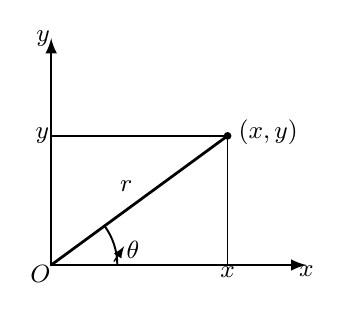
\begin{tikzpicture}[x=0.80cm, y=0.80cm, >=latex, line cap=round, line join=round]
  \draw[line width=0.9pt, ->] (0, 0) -- (4.05, 0) node[below=-1pt, inner sep=1pt] {\small $x$};
  \draw[line width=0.9pt, ->] (0, 0) -- (0, 3.60) node[left=-1pt, inner sep=1pt] {\small $y$};
  \node[below left=-1pt, inner sep=1pt] at (0, 0) {\small $O$};
  % 投影辅助线
  \draw[line width=0.6pt] (0, 2.05) -- (2.80, 2.05);
  \draw[line width=0.6pt] (2.80, 0) -- (2.80, 2.05);
  % 半径 r
  \draw[line width=1.0pt] (0, 0) -- (2.80, 2.05);
  \node[above left=-1pt, inner sep=1.5pt] at (1.32, 1.14) {\small $r$};
  % 夹角 theta
  \draw[line width=0.7pt] (1.05, 0) arc[start angle=0, end angle=36.2, radius=1.05];
  \draw[->, line width=0.5pt] (1.00, 0.06) -- (1.16, 0.30);
  \node[inner sep=1pt] at (1.30, 0.24) {\small $\theta$};
  % 端点
  \fill (2.80, 2.05) circle (1.4pt);
  \node[anchor=west, inner sep=1.5pt] at (2.90, 2.10) {\small $(x,y)$};
  \node[left=-1pt, inner sep=1.5pt] at (0, 2.05) {\small $y$};
  \node[below=-1pt, inner sep=1.5pt] at (2.80, 0) {\small $x$};
\end{tikzpicture}
\caption{}\label{fig:8.4.2}
\end{figure}

因此，$f$ 为局部 $C^{\infty}$ 微分同胚。但由 $f(1,0) = f(1,2\pi)$ 知 $f$ 非单射，从而整体的 $f^{-1}$ 不存在，$f$ 不为整体 $C^{\infty}$ 微分同胚。

再求 $r$，$\theta$ 关于 $x$，$y$ 的偏导数 $\dfrac{\partial r}{\partial x}$，$\dfrac{\partial r}{\partial y}$，$\dfrac{\partial\theta}{\partial x}$，$\dfrac{\partial\theta}{\partial y}$.
\end{example}

\begin{proof}[解法 1]
\begin{align*}
  \boldsymbol{J}f^{-1}(x,y) &= \bigl[\boldsymbol{J}f(\boldsymbol{r},\boldsymbol{\theta})\bigr]^{-1} \\
  &= \begin{pmatrix} \dfrac{\partial r}{\partial x} & \dfrac{\partial r}{\partial y} \\[6pt] \dfrac{\partial\theta}{\partial x} & \dfrac{\partial\theta}{\partial y} \end{pmatrix} = \begin{pmatrix} \dfrac{\partial x}{\partial r} & \dfrac{\partial x}{\partial\theta} \\[6pt] \dfrac{\partial y}{\partial r} & \dfrac{\partial y}{\partial\theta} \end{pmatrix}^{-1} = \begin{pmatrix} \cos\theta & -r\sin\theta \\ \sin\theta & r\cos\theta \end{pmatrix}^{-1} \\
  &= \frac{1}{r}\begin{pmatrix} r\cos\theta & r\sin\theta \\ -\sin\theta & \cos\theta \end{pmatrix} = \begin{pmatrix} \dfrac{x}{\sqrt{x^{2}+y^{2}}} & \dfrac{y}{\sqrt{x^{2}+y^{2}}} \\[8pt] -\dfrac{y}{x^{2}+y^{2}} & \dfrac{x}{x^{2}+y^{2}} \end{pmatrix}.
\end{align*}
\end{proof}

\begin{proof}[解法 2]
$r = \sqrt{x^{2}+y^{2}}$，$\theta = \arctan\dfrac{y}{x}$，因此
\[
  \frac{\partial r}{\partial x} = \frac{x}{\sqrt{x^{2}+y^{2}}},\quad \frac{\partial r}{\partial y} = \frac{y}{\sqrt{x^{2}+y^{2}}},
\]
\[
  \frac{\partial\theta}{\partial x} = \frac{-\dfrac{y}{x^{2}}}{1 + \left(\dfrac{y}{x}\right)^{2}} = -\frac{y}{x^{2}+y^{2}},\quad \frac{\partial\theta}{\partial y} = \frac{\dfrac{1}{x}}{1 + \left(\dfrac{y}{x}\right)^{2}} = \frac{x}{x^{2}+y^{2}}.
\]
\end{proof}

\begin{example}\label{ex:8.4.13}
设 $f: (0,+\infty) \times (0,\pi) \times (-\infty,+\infty) \to \mathbb{R}^{3}$，
\[
  (r,\theta,\varphi) \mapsto (x,y,z) = f(r,\theta,\varphi) = (r\sin\theta\cos\varphi,r\sin\theta\sin\varphi,r\cos\theta)
\]
为球坐标变换公式(图 8.4.3)，则
\begin{align*}
  \det \boldsymbol{J}f(\boldsymbol{r},\boldsymbol{\theta},\boldsymbol{\varphi}) &= \frac{\partial(x,y,z)}{\partial(r,\theta,\varphi)} = \begin{vmatrix} \dfrac{\partial x}{\partial r} & \dfrac{\partial x}{\partial\theta} & \dfrac{\partial x}{\partial\varphi} \\[6pt] \dfrac{\partial y}{\partial r} & \dfrac{\partial y}{\partial\theta} & \dfrac{\partial y}{\partial\varphi} \\[6pt] \dfrac{\partial z}{\partial r} & \dfrac{\partial z}{\partial\theta} & \dfrac{\partial z}{\partial\varphi} \end{vmatrix} \\
  &= \begin{vmatrix} \sin\theta\cos\varphi & r\cos\theta\cos\varphi & -r\sin\theta\sin\varphi \\ \sin\theta\sin\varphi & r\cos\theta\sin\varphi & r\sin\theta\cos\varphi \\ \cos\theta & -r\sin\theta & 0 \end{vmatrix} = r^{2}\sin\theta \neq 0.
\end{align*}

\begin{figure}[htbp]
\centering
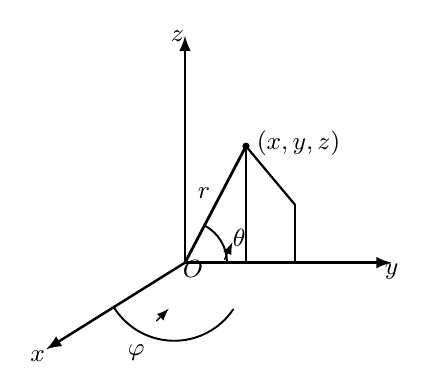
\begin{tikzpicture}[x=0.86cm, y=0.86cm, >=latex, line cap=round, line join=round]
  % 三轴
  \draw[line width=0.9pt, ->] (0, 0) -- (3.05, 0) node[below=-1pt, inner sep=1pt] {\small $y$};
  \draw[line width=0.9pt, ->] (0, 0) -- (0, 3.35) node[left=-1pt, inner sep=1pt] {\small $z$};
  \draw[line width=0.9pt, ->] (0, 0) -- (-2.05, -1.28) node[below left=-1pt, inner sep=1pt] {\small $x$};
  \node[below right=-2pt, inner sep=1pt] at (0, 0) {\small $O$};
  % 竖直投影三角形(母线)
  \draw[line width=0.8pt] (0.90, 0) -- (0.90, 1.72);
  \draw[line width=0.8pt] (0.90, 1.72) -- (1.62, 0.86);
  \draw[line width=0.8pt] (1.62, 0.86) -- (1.62, 0);
  % 半径 r
  \draw[line width=1.0pt] (0, 0) -- (0.90, 1.72);
  \node[above left=-1pt, inner sep=1.5pt] at (0.40, 0.92) {\small $r$};
  % theta 角
  \draw[line width=0.7pt] (0.62, 0) arc[start angle=0, end angle=62.4, radius=0.62];
  \draw[->, line width=0.5pt] (0.585, 0.05) -- (0.70, 0.30);
  \node[inner sep=1pt] at (0.80, 0.36) {\small $\theta$};
  % phi 角
  \draw[line width=0.7pt] (-1.05, -0.66) arc[start angle=212, end angle=326, radius=1.05];
  \draw[->, line width=0.5pt] (-0.42, -0.86) -- (-0.24, -0.68);
  \node[below=-1pt, inner sep=1pt] at (-0.72, -1.20) {\small $\varphi$};
  % 点 (x,y,z)
  \fill (0.90, 1.72) circle (1.3pt);
  \node[anchor=west, inner sep=1.5pt] at (0.99, 1.76) {\small $(x,y,z)$};
\end{tikzpicture}
\caption{}\label{fig:8.4.3}
\end{figure}

因此，$f$ 为局部 $C^{\infty}$ 微分同胚。但由 $f\left(1,\dfrac{\pi}{2},0\right) = f\left(1,\dfrac{\pi}{2},2\pi\right)$ 知，$f$ 非单射，从而整体的 $f^{-1}$ 不存在，$f$ 不为整体的 $C^{\infty}$ 微分同胚。
\end{example}

\begin{proof}[解法 1]
\begin{align*}
  \boldsymbol{J}f^{-1}(x,y,z) &= \bigl[\boldsymbol{J}f(\boldsymbol{r},\boldsymbol{\theta},\boldsymbol{\varphi})\bigr]^{-1} \\
  &= \begin{pmatrix} \dfrac{\partial r}{\partial x} & \dfrac{\partial r}{\partial y} & \dfrac{\partial r}{\partial z} \\[6pt] \dfrac{\partial\theta}{\partial x} & \dfrac{\partial\theta}{\partial y} & \dfrac{\partial\theta}{\partial z} \\[6pt] \dfrac{\partial\varphi}{\partial x} & \dfrac{\partial\varphi}{\partial y} & \dfrac{\partial\varphi}{\partial z} \end{pmatrix} \\
  &= \begin{pmatrix} \dfrac{\partial x}{\partial r} & \dfrac{\partial x}{\partial\theta} & \dfrac{\partial x}{\partial\varphi} \\[6pt] \dfrac{\partial y}{\partial r} & \dfrac{\partial y}{\partial\theta} & \dfrac{\partial y}{\partial\varphi} \\[6pt] \dfrac{\partial z}{\partial r} & \dfrac{\partial z}{\partial\theta} & \dfrac{\partial z}{\partial\varphi} \end{pmatrix}^{-1} \\
  &= \begin{pmatrix} \sin\theta\cos\varphi & r\cos\theta\cos\varphi & -r\sin\theta\sin\varphi \\ \sin\theta\sin\varphi & r\cos\theta\sin\varphi & r\sin\theta\cos\varphi \\ \cos\theta & -r\sin\theta & 0 \end{pmatrix}^{-1} \\
  &= \frac{1}{r^{2}\sin\theta}\begin{pmatrix} r^{2}\sin^{2}\theta\cos\varphi & r^{2}\sin^{2}\theta\sin\varphi & r^{2}\sin\theta\cos\theta \\ r\sin\theta\cos\theta\cos\varphi & r\sin\theta\cos\theta\sin\varphi & -r\sin^{2}\theta \\ -r\sin\varphi & r\cos\varphi & 0 \end{pmatrix} \\
  &= \begin{pmatrix} \sin\theta\cos\varphi & \sin\theta\sin\varphi & \cos\theta \\[4pt] \dfrac{\cos\theta\cos\varphi}{r} & \dfrac{\cos\theta\sin\varphi}{r} & -\dfrac{\sin\theta}{r} \\[8pt] -\dfrac{\sin\varphi}{r\sin\theta} & \dfrac{\cos\varphi}{r\sin\theta} & 0 \end{pmatrix} \\
  &= \begin{pmatrix} \dfrac{x}{r} & \dfrac{y}{r} & \dfrac{z}{r} \\[8pt] \dfrac{xz}{r^{2}\sqrt{x^{2}+y^{2}}} & \dfrac{yz}{r^{2}\sqrt{x^{2}+y^{2}}} & -\dfrac{\sqrt{x^{2}+y^{2}}}{r^{2}} \\[8pt] -\dfrac{y}{x^{2}+y^{2}} & \dfrac{x}{x^{2}+y^{2}} & 0 \end{pmatrix},
\end{align*}
其中 $x^{2}+y^{2} = r^{2}\sin^{2}\theta \neq 0$，$r = \sqrt{x^{2}+y^{2}+z^{2}} \neq 0$，
\[
  r = \sqrt{x^{2}+y^{2}+z^{2}},\quad \theta = \arccos\frac{z}{\sqrt{x^{2}+y^{2}+z^{2}}},\quad \varphi = \arcsin\frac{y}{\sqrt{x^{2}+y^{2}}}.
\]
通过简单计算，分别求出 $r$，$\theta$，$\varphi$ 对于 $x$，$y$，$z$ 的偏导数可以验证与上述结果完全一致.
\end{proof}

\begin{example}\label{ex:8.4.14}
设 $U \subset \mathbb{R}^{4}$ 为开集，$F$，$G: U \to \mathbb{R}^{1}$ 为 4 元函数。如果 $\boldsymbol{H} = (F,G)^{\mathrm{T}}$ 在点 $(z_{0},w_{0}) \in U$ (其中 $z_{0} = (x_{0},y_{0})$，$w_{0} = (u_{0},v_{0})$) 的某开邻域内满足隐射定理 8.4.2 的条件且 $\det \boldsymbol{J}_{w}H(z_{0},w_{0}) \neq 0$，则方程组 $\boldsymbol{H}(x,y,u,v) = \boldsymbol{0}$ 在点 $z_{0}$ 的某开邻域内能确定一个 $C^{k}$ 隐映 $w = f(z)$.
\end{example}

\begin{proof}[解法 1]
由定理 8.4.2 中的 (4) 求得
\[
  \boldsymbol{J}f(\boldsymbol{z}) = -\bigl[\boldsymbol{J}_{w}\boldsymbol{H}(\boldsymbol{z},\boldsymbol{w})\bigr]^{-1}\boldsymbol{J}_{z}\boldsymbol{H}(\boldsymbol{z},\boldsymbol{w}),
\]
即
\[
  \begin{pmatrix} \dfrac{\partial u}{\partial x} & \dfrac{\partial u}{\partial y} \\[6pt] \dfrac{\partial v}{\partial x} & \dfrac{\partial v}{\partial y} \end{pmatrix} = -\begin{pmatrix} \dfrac{\partial F}{\partial u} & \dfrac{\partial F}{\partial v} \\[6pt] \dfrac{\partial G}{\partial u} & \dfrac{\partial G}{\partial v} \end{pmatrix}^{-1}\begin{pmatrix} \dfrac{\partial F}{\partial x} & \dfrac{\partial F}{\partial y} \\[6pt] \dfrac{\partial G}{\partial x} & \dfrac{\partial G}{\partial y} \end{pmatrix}
\]
\begin{align*}
  &= -\frac{-1}{J}\begin{pmatrix} \dfrac{\partial G}{\partial v} & -\dfrac{\partial F}{\partial v} \\[6pt] -\dfrac{\partial G}{\partial u} & \dfrac{\partial F}{\partial u} \end{pmatrix}\begin{pmatrix} \dfrac{\partial F}{\partial x} & \dfrac{\partial F}{\partial y} \\[6pt] \dfrac{\partial G}{\partial x} & \dfrac{\partial G}{\partial y} \end{pmatrix} \\
  &= -\frac{1}{J}\begin{pmatrix} \dfrac{\partial(F,G)}{\partial(x,v)} & \dfrac{\partial(F,G)}{\partial(y,v)} \\[6pt] \dfrac{\partial(F,G)}{\partial(u,x)} & \dfrac{\partial(F,G)}{\partial(u,y)} \end{pmatrix},
\end{align*}
其中 $J = \dfrac{\partial(F,G)}{\partial(u,v)}$.
\end{proof}

\begin{proof}[解法 2]
设 $u = f(x,y)$，$v = g(x,y)$ 为由方程组
\[
  \left\{\begin{aligned}
    F(x,y,u,v) &= 0, \\
    G(x,y,u,v) &= 0
  \end{aligned}\right.
\]
所确定的隐函数，即
\[
  \left\{\begin{aligned}
    F(x,y,f(x,y),g(x,y)) &\equiv 0, \\
    G(x,y,f(x,y),g(x,y)) &\equiv 0.
  \end{aligned}\right.
\]
对上述方程组关于 $x$，$y$ 分别求偏导数得到
\begin{align*}
  &\left\{\begin{aligned}
    F_{x}^{\prime} + F_{u}^{\prime}u_{x}^{\prime} + F_{v}^{\prime}v_{x}^{\prime} &= 0, \\
    G_{x}^{\prime} + G_{u}^{\prime}u_{x}^{\prime} + G_{v}^{\prime}v_{x}^{\prime} &= 0,
  \end{aligned}\right. \\
  &\left\{\begin{aligned}
    F_{y}^{\prime} + F_{u}^{\prime}u_{y}^{\prime} + F_{v}^{\prime}v_{y}^{\prime} &= 0, \\
    G_{y}^{\prime} + G_{u}^{\prime}u_{y}^{\prime} + G_{v}^{\prime}v_{y}^{\prime} &= 0.
  \end{aligned}\right.
\end{align*}
因为
\[
  J = \frac{\partial(F,G)}{\partial(u,v)} = \begin{vmatrix} F_{u}^{\prime} & F_{v}^{\prime} \\ G_{u}^{\prime} & G_{v}^{\prime} \end{vmatrix} \neq 0,
\]
故从两个方程组分别解得
\[
  \frac{\partial u}{\partial x} = u_{x}^{\prime} = -\frac{1}{J}\frac{\partial(F,G)}{\partial(x,v)},\quad \frac{\partial u}{\partial y} = u_{y}^{\prime} = -\frac{1}{J}\frac{\partial(F,G)}{\partial(y,v)},
\]
\[
  \frac{\partial v}{\partial x} = v_{x}^{\prime} = -\frac{1}{J}\frac{\partial(F,G)}{\partial(u,x)},\quad \frac{\partial v}{\partial y} = v_{y}^{\prime} = -\frac{1}{J}\frac{\partial(F,G)}{\partial(u,y)}.
\]
\end{proof}

\begin{exblock}{练习题 8.4}
\item 下列方程确定隐函数 $y = y(x)$，计算 $\dfrac{\mathrm{d}y}{\mathrm{d}x}$;
\begin{enumerate}
  \item[(1)] $x^{2} + 2xy - y^{2} = a^{2}$;
  \item[(2)] $xy - \ln y = 0$，在点 $(0,1)$ 处;
  \item[(3)] $y - \varepsilon \sin y = x$，常数 $\varepsilon \in (0,1)$;
  \item[(4)] $x^{y} = y^{x}$
\end{enumerate}

\item 下列方程确定隐函数 $z = z(x,y)$，计算 $\dfrac{\partial z}{\partial x}$ 与 $\dfrac{\partial z}{\partial y}$.
\begin{enumerate}
  \item[(1)] $e^{x} - xyz = 0$;
  \item[(2)] $\dfrac{x}{z} = \ln\dfrac{z}{y}$;
  \item[(3)] $x + y + z = e^{-(x+y+z)}$，并对计算的结果作出解释;
  \item[(4)] $z^{2}y - xz^{3} - 1 = 0$，在点 $(1,2,1)$ 处.
\end{enumerate}

\item 设 $u = f(x,y,z,t)$，$g(y,z,t) = 0$，$h(z,t) = 0$，$f$，$g$ 与 $h$ 都一阶连续可导，计算 $\dfrac{\partial u}{\partial x}$ 与 $\dfrac{\partial u}{\partial y}$，并给出相应可计算的条件.

\item 设 $F(x-y,y-z,z-x) = 0$，$F$ 有一阶连续偏导数，计算 $\dfrac{\partial z}{\partial x}$ 与 $\dfrac{\partial z}{\partial y}$，并给出相应可计算的条件.

\item 设 $F(x+y+z,x^{2}+y^{2}+z^{2}) = 0$，$F$ 有一阶连续偏导数，计算 $\dfrac{\partial z}{\partial x}$ 与 $\dfrac{\partial z}{\partial y}$，并给出相应可计算的条件.

\item 二元函数 $F$ 在 $\mathbb{R}^{2}$ 上二次连续可导. 已知曲线 $F(x,y) = 0$ 呈“8”字形. 问方程组
\[
  \begin{cases}
    \dfrac{\partial F}{\partial x}(x,y) = 0, \\[4pt]
    \dfrac{\partial F}{\partial y}(x,y) = 0
  \end{cases}
\]
在 $\mathbb{R}^{2}$ 中至少有几组解?

\item 从方程组
\[
  \left\{\begin{aligned}
    x^{2} + y^{2} + z^{2} &= 1, \\
    x + y + z &= 0
  \end{aligned}\right.
\]
中，计算 $\dfrac{\mathrm{d}y}{\mathrm{d}x}$ 与 $\dfrac{\mathrm{d}z}{\mathrm{d}x}$，并作出几何解释.

\item 从方程组
\[
  \left\{\begin{aligned}
    x^{2} + y^{2} - z &= 0, \\
    x^{2} + 2y^{2} + 3z^{2} &= 20
  \end{aligned}\right.
\]
中，计算 $\dfrac{\mathrm{d}y}{\mathrm{d}x}$ 与 $\dfrac{\mathrm{d}z}{\mathrm{d}x}$，并作出几何解释.

\item 从下列方程中，计算 Jacobi 矩阵
\[
  \begin{pmatrix} \dfrac{\partial x}{\partial u} & \dfrac{\partial x}{\partial v} \\[6pt] \dfrac{\partial y}{\partial u} & \dfrac{\partial y}{\partial v} \end{pmatrix}.
\]
\begin{enumerate}
  \item[(1)] $xu - yv = 0$，$yu + xv = 1$;
  \item[(2)] $x + y = u + v$，$\dfrac{x}{y} = \dfrac{\sin u}{\sin v}$.
\end{enumerate}

\item 设
\[
  \left\{\begin{aligned}
    u^{2} - v\cos(xy) + w^{2} &= 0, \\
    u^{2} + v^{2} - \sin(xy) + 2w^{2} &= 2, \\
    uv - \sin x \cos y + w &= 0,
  \end{aligned}\right.
\]
试在 $(x,y) = \left(\dfrac{\pi}{2},0\right)$，$(u,v,w) = (1,1,0)$ 处计算 Jacobi 矩阵
\[
  \begin{pmatrix} \dfrac{\partial u}{\partial x} & \dfrac{\partial u}{\partial y} \\[6pt] \dfrac{\partial v}{\partial x} & \dfrac{\partial v}{\partial y} \\[6pt] \dfrac{\partial w}{\partial x} & \dfrac{\partial w}{\partial y} \end{pmatrix}.
\]

\item 从方程组
\[
  \left\{\begin{aligned}
    x &= t + \dfrac{1}{t}, \\
    y &= t^{2} + \dfrac{1}{t^{2}}, \\
    z &= t^{3} + \dfrac{1}{t^{3}}
  \end{aligned}\right.
\]
中，计算 $\dfrac{\mathrm{d}y}{\mathrm{d}x}$ 与 $\dfrac{\mathrm{d}z}{\mathrm{d}x}$.

\item 设 $U \subset \mathbb{R}^{n}$，$f: U \to \mathbb{R}^{n}$. 如果 $f$ 将开集映为开集，则称 $f$ 为一个开映射。问: 下列映射是否为开映射? 并说明理由。
\begin{enumerate}
  \item[(1)] $f(x,y) = \left(x^{2},\dfrac{y}{x}\right)$;
  \item[(2)] $f(x,y) = \left(\mathrm{e}^{x}\cos y,\mathrm{e}^{x}\sin y\right)$;
  \item[(3)] $f(x,y) = (x,x^{2})$
\end{enumerate}
进而，对 (1) 与 (2) 中的 $f$，计算 $\boldsymbol{J}f^{-1}$

\item 求由下列方程所确定的隐函数的偏导数:
\begin{enumerate}
  \item[(1)] $x + y + z = \mathrm{e}^{-(x+y+z)}$，求 $z$ 对 $x$，$y$ 的一阶与二阶偏导数;
  \item[(2)] $F(x,x+y,x+y+z) = 0$，$F$ 为 $C^{2}$ 函数，求 $\dfrac{\partial z}{\partial x}$，$\dfrac{\partial z}{\partial y}$，$\dfrac{\partial^{2} z}{\partial x^{2}}$.
\end{enumerate}

\item 设 $f$ 为一元函数，试问: $f$ 应满足什么条件，方程 $2f(xy) = f(x) + f(y)$ 在点 $(1,1)$ 的开邻域内能确定出惟一的 $y$ 为 $x$ 的函数?

\item 设 $F(x,y)$ 为 $C^{2}$ 函数，$F_{y}^{\prime} \neq 0$，证明: 由 $F(x,y) = 0$ 所确定的隐函数 $y = f(x)$ 有
\[
  \left(F_{y}^{\prime}\right)^{3} y'' = \begin{vmatrix} F_{xx}^{\prime\prime} & F_{xy}^{\prime\prime} & F_{x}^{\prime} \\ F_{xy}^{\prime\prime} & F_{yy}^{\prime\prime} & F_{y}^{\prime} \\ F_{x}^{\prime} & F_{y}^{\prime} & 0 \end{vmatrix}.
\]

\item 求由下列方程所确定的隐函数的极值:
\begin{enumerate}
  \item[(1)] $x^{2} + 2xy + 2y^{2} = 1$
  \item[(2)] $(x^{2}+y^{2}) = a^{2}(x^{2}-y^{2})$ $(a > 0)$
\end{enumerate}

\item 设 $f$，$g$，$h$ 可微，
\[
  \begin{cases}
    x = f(u,v,w), \\
    y = g(u,v,w), \\
    z = h(u,v,w),
  \end{cases}
\]
求 $\dfrac{\partial u}{\partial x}$，$\dfrac{\partial u}{\partial y}$，$\dfrac{\partial u}{\partial z}$，并给出可计算的条件.

\item 设 $f$，$g$ 为可微函数，求下列方程所确定的隐函数 $u = u(x,y)$ 的偏导数 $\dfrac{\partial u}{\partial x}$，$\dfrac{\partial u}{\partial y}$
\begin{enumerate}
  \item[(1)] $x^{2} + u^{2} = f(x,u) + g(x,y,u)$;
  \item[(2)] $u = f(x + u,yu)$.
\end{enumerate}
进而给出可计算的条件.

\item 设 $y = f(x)$ 为 $C^{1}$ 函数，$x = \varphi(u,v)$，$y = \psi(u,v)$ 为 $C^{2}$ 函数，则由方程 $\psi(u,v) = f(\varphi(u,v))$ 可以确定函数 $v = v(u)$. 试用 $u$，$v$，$\dfrac{\mathrm{d}v}{\mathrm{d}u}$，$\dfrac{\mathrm{d}^{2}v}{\mathrm{d}u^{2}}$ 表示 $\dfrac{\mathrm{d}y}{\mathrm{d}x}$，$\dfrac{\mathrm{d}^{2}y}{\mathrm{d}x^{2}}$; 并给出可计算的条件.
\end{exblock}

\begin{exblock}{思考题 8.4}
\item 设 $(x_{0},y_{0},z_{0},u_{0})$ 满足方程组
\[
  \left\{\begin{aligned}
    f(x) + f(y) + f(z) &= F(u), \\
    g(x) + g(y) + g(z) &= G(u), \\
    h(x) + h(y) + h(z) &= H(u),
  \end{aligned}\right.
\]
这里所有的函数假定有连续的导数.

(1) 说出一个能在该点开邻域内确定 $x$，$y$，$z$ 为 $u$ 的函数的充分条件;

(2) 在 $f(x) = x$，$g(x) = x^{2}$，$h(x) = x^{3}$ 的情形下，上述条件相当于什么?

\item 据理说明: 在点 $(0,1)$ 近旁是否存在 $C^{\infty}$ 的 $f(x,y)$ 与 $g(x,y)$ 满足:
\[
  f(0,1) = 1,\quad g(0,1) = -1,
\]
且
\[
  \left\{\begin{aligned}
    [f(x,y)]^{3} + x g(x,y) - y &= 0, \\
    [g(x,y)]^{3} + y f(x,y) - x &= 0.
  \end{aligned}\right.
\]
\end{exblock}


\section{逆射与隐射定理的另一精美证法}\label{sec:8.5}

上节应用数学归纳法先证隐射定理: 方程组 $F(x,y) = 0$ 在条件 $\det J_{y}F \neq 0$ 时, 局部解得 $y = f(x)$, 使得 $F(x,f(x)) \equiv 0$. 进而, 当 $\det Jf(x) \neq 0$ 时, 对 $F(x,y) = f(x) - y = 0$ 施用隐射定理, 证得 $y = f(x)$ 有局部逆射 $x = g(y) = f^{-1}(y)$. 读者已领略了它的精美的论证方法. 自然会大胆地问: 能否先证局部逆射定理, 再应用局部逆射定理来证明隐射定理? 现在来实现这一设想.

\begin{theorem}[局部逆射定理]\label{thm:8.5.1}
设 $D \subset \mathbb{R}^{n}$ 为开集, $f: D \to \mathbb{R}^{n}$ 为 $C^{k}$ $(1 \leqslant k \leqslant +\infty)$ 映射, 且
\[
  \det Jf(\boldsymbol{x}^{0}) = \det\left(\frac{\partial f_{i}}{\partial x_{j}}(\boldsymbol{x}^{0})\right) \neq 0, \quad \boldsymbol{x}^{0} \in D,
\]
则 $f$ 为一个 $C^{k}$ 局部微分同胚, 它将 $\boldsymbol{x}^{0}$ 的一个开邻域映成 $f(\boldsymbol{x}^{0})$ 的一个开邻域.
\end{theorem}

\begin{proof}
可以假定 $\boldsymbol{x}^{0} = \boldsymbol{0}$, $f(\boldsymbol{x}^{0}) = \boldsymbol{0}$, $\left(\dfrac{\partial f_{i}}{\partial x_{j}}(\boldsymbol{x}^{0})\right) = (\delta_{j}^{i}) = \boldsymbol{I}$ (否则作一仿射变换, 不影响定理的证明). 选 $a$ 充分小, 使得方体
\[
  C^{n}(a) = \bigl\{\boldsymbol{x} \in \mathbb{R}^{n} \mid \|\boldsymbol{x}\| = \max_{1 \leqslant j \leqslant n}|x_{j}| < a\bigr\} \subset D,
\]
且当 $\boldsymbol{x} \in C^{n}(a)$ 时,
\[
  \det\left(\frac{\partial f_{i}}{\partial x_{j}}(\boldsymbol{x})\right) \neq 0
\]
及
\[
  \left(\frac{\partial f_{i}}{\partial x_{j}}(\boldsymbol{x})\right) - \boldsymbol{I}
\]
中的元素满足
\[
  \left|\left(\frac{\partial f_{i}}{\partial x_{j}}(\boldsymbol{x})\right) - \delta_{j}^{i}\right| \leqslant \frac{1}{2n}
  \quad \biggl(\text{只需注意}\ \left(\frac{\partial f_{i}}{\partial x_{j}}(\boldsymbol{0})\right) - \boldsymbol{I} = \boldsymbol{0}\biggr).
\]
令 $g(\boldsymbol{x}) = f(\boldsymbol{x}) - \boldsymbol{x}$, 则当 $\boldsymbol{x}^{1}, \boldsymbol{x}^{2} \in C^{n}(a)$ 时, 应用 Lagrange 中值定理有
\begin{align*}
  \|\boldsymbol{g}(\boldsymbol{x}^{1}) - \boldsymbol{g}(\boldsymbol{x}^{2})\| &= \max_{1 \leqslant i \leqslant n}\bigl\{|g_{i}(\boldsymbol{x}^{1}) - g_{i}(\boldsymbol{x}^{2})|\bigr\} \\
  &= \max_{1 \leqslant i \leqslant n}\left\{\left|\sum_{j=1}^{n}\frac{\partial g_{i}}{\partial x_{j}}(\boldsymbol{\xi}^{j})(x_{j}^{1} - x_{j}^{2})\right|\right\} \\
  &\leqslant n\max_{1 \leqslant i, j \leqslant n}\left\{\left|\frac{\partial g_{i}}{\partial x_{j}}(\boldsymbol{\xi}^{j})\right|\right\}\max_{1 \leqslant j \leqslant n}\bigl\{|x_{j}^{1} - x_{j}^{2}|\bigr\} \\
  &\leqslant n \cdot \frac{1}{2n}\|\boldsymbol{x}^{1} - \boldsymbol{x}^{2}\| = \frac{1}{2}\|\boldsymbol{x}^{1} - \boldsymbol{x}^{2}\|.
\end{align*}
此外, 还有
\begin{align*}
  \|f(\boldsymbol{x}^{1}) - f(\boldsymbol{x}^{2})\| &= \|\boldsymbol{g}(\boldsymbol{x}^{1}) - \boldsymbol{g}(\boldsymbol{x}^{1}) + \boldsymbol{x}^{1} - \boldsymbol{x}^{2}\| \\
  &\geqslant \|\boldsymbol{x}^{1} - \boldsymbol{x}^{2}\| - \|\boldsymbol{g}(\boldsymbol{x}^{1}) - \boldsymbol{g}(\boldsymbol{x}^{2})\| \\
  &\geqslant \|\boldsymbol{x}^{1} - \boldsymbol{x}^{2}\| - \frac{1}{2}\|\boldsymbol{x}^{1} - \boldsymbol{x}^{2}\| \\
  &= \frac{1}{2}\|\boldsymbol{x}^{1} - \boldsymbol{x}^{2}\|.
\end{align*}
\begin{enumerate}
\item[(1)] 如果 $\boldsymbol{y} \in C^{n}\left(\dfrac{a}{2}\right)$, 则必存在一点 $\boldsymbol{x} \in C^{n}(a)$, 使得 $f(\boldsymbol{x}) = \boldsymbol{y}$.

为此, 设
\[
  \boldsymbol{x}^{0} = \boldsymbol{0}, \quad \boldsymbol{x}^{1} = \boldsymbol{y}, \quad \boldsymbol{x}^{k+1} = \boldsymbol{y} - \boldsymbol{g}(\boldsymbol{x}^{k}), \quad k = 0, 1, 2, \cdots,
\]
容易看出
\begin{align*}
  \|\boldsymbol{x}^{k} - \boldsymbol{x}^{k-1}\| &= \|\boldsymbol{g}(\boldsymbol{x}^{k-1}) - \boldsymbol{g}(\boldsymbol{x}^{k-2})\| \leqslant \frac{1}{2}\|\boldsymbol{x}^{k-1} - \boldsymbol{x}^{k-2}\| \\
  \leqslant {} & \cdots \leqslant \frac{1}{2^{k-2}}\|\boldsymbol{x}^{1} - \boldsymbol{x}^{0}\| = \frac{1}{2^{k-1}}\|\boldsymbol{y}\|,
\end{align*}
\begin{align*}
  \|\boldsymbol{x}^{k}\| &= \|\boldsymbol{x}^{k} - \boldsymbol{x}^{0}\| \\
  &\leqslant \|\boldsymbol{x}^{k} - \boldsymbol{x}^{k-1}\| + \|\boldsymbol{x}^{k-1} - \boldsymbol{x}^{k-2}\| + \cdots + \|\boldsymbol{x}^{1} - \boldsymbol{x}^{0}\| \\
  &\leqslant \left(\frac{1}{2^{k-1}} + \frac{1}{2^{k-2}} + \cdots + 1\right)\|\boldsymbol{y}\| < 2\|\boldsymbol{y}\| < 2 \cdot \frac{a}{2} = a,
\end{align*}
\begin{align*}
  \|\boldsymbol{x}^{k+p} - \boldsymbol{x}^{k}\| &\leqslant \|\boldsymbol{x}^{k+p} - \boldsymbol{x}^{k+p-1}\| + \cdots + \|\boldsymbol{x}^{k+1} - \boldsymbol{x}^{k}\| \\
  &\leqslant \left(\frac{1}{2^{k+p-1}} + \cdots + \frac{1}{2^{k}}\right)\|\boldsymbol{y}\| \\
  &= \frac{1}{2^{k}}\left(\frac{1}{2^{p-1}} + \cdots + 1\right)\|\boldsymbol{y}\| \leqslant \frac{1}{2^{k-1}}\|\boldsymbol{y}\|.
\end{align*}
于是, $\boldsymbol{x}^{k} \in C^{n}(a)$ 及 $\{\boldsymbol{x}^{k}\}$ 为 Cauchy 点列. 由于 $\mathbb{R}^{n}$ 完备, 故 $\{\boldsymbol{x}^{k}\}$ 收敛, 设 $\lim\limits_{k \to +\infty}\boldsymbol{x}^{k} = \boldsymbol{x}$, 再在上述第二个不等式中令 $k \to +\infty$ 得到
\[
  \|\boldsymbol{x}\| < 2\|\boldsymbol{y}\| < a,
\]
因而 $\boldsymbol{x} \in C^{n}(a)$, 且
\begin{align*}
  \boldsymbol{x} &= \lim_{k \to +\infty}\boldsymbol{x}^{k+1} = \lim_{k \to +\infty}\bigl[\boldsymbol{y} - \boldsymbol{g}(\boldsymbol{x}^{k})\bigr] = \boldsymbol{y} - \boldsymbol{g}(\boldsymbol{x}) \\
  &= \boldsymbol{y} - \bigl[f(\boldsymbol{x}) - \boldsymbol{x}\bigr] = \boldsymbol{y} - f(\boldsymbol{x}) + \boldsymbol{x}, \quad f(\boldsymbol{x}) = \boldsymbol{y}.
\end{align*}
这就证明了 $\boldsymbol{x}$ 的存在性.

再证惟一性. 如果 $\exists\,\boldsymbol{x}, \boldsymbol{x}' \in C^{n}(a)$, s. t.\ $f(\boldsymbol{x}) = \boldsymbol{y} = f(\boldsymbol{x}')$, 则由
\[
  0 = \|f(\boldsymbol{x}) - f(\boldsymbol{x}')\| \geqslant \frac{1}{2}\|\boldsymbol{x} - \boldsymbol{x}'\| \geqslant 0,
\]
推得 $\|\boldsymbol{x} - \boldsymbol{x}'\| = 0$, $\boldsymbol{x} = \boldsymbol{x}'$.

\item[(2)] 由 (1) 知 $f^{-1}: C^{n}\left(\dfrac{a}{2}\right) \to C^{n}(a)$ 是存在的. 另一方面, 从
\[
  \|\boldsymbol{y}' - \boldsymbol{y}''\| = \|f(\boldsymbol{x}') - f(\boldsymbol{x}'')\| \geqslant \frac{1}{2}\|\boldsymbol{x}' - \boldsymbol{x}''\| = \frac{1}{2}\|f^{-1}(\boldsymbol{y}') - f^{-1}(\boldsymbol{y}'')\|
\]
可推出 $f^{-1}$ 在 $C^{n}\left(\dfrac{a}{2}\right)$ 上是一致连续的, 因而是连续的.

显然, 由 $f$ 连续及 $C^{n}\left(\dfrac{a}{2}\right)$ 为开集知, $f^{-1}\left(C^{n}\left(\dfrac{a}{2}\right)\right)$ 为开集, 从而 $C^{n}\left(\dfrac{a}{2}\right)$ 在 $f^{-1}: C^{n}\left(\dfrac{a}{2}\right) \to C^{n}(a)$ 下的逆像为 $C^{n}(a) \cap f^{-1}\left(C^{n}\left(\dfrac{a}{2}\right)\right)$, 它是开集. 这就证明了
\[
  f: C^{n}(a) \cap f^{-1}\left(C^{n}\left(\frac{a}{2}\right)\right) \to C^{n}\left(\frac{a}{2}\right)
\]
为一个同胚 (拓扑映射), 它将 $\boldsymbol{0}$ 的一个开邻域映成 $f(\boldsymbol{0}) = \boldsymbol{0}$ 的一个开邻域.

\item[(3)] $f^{-1}$ 是可微的, 由此得到 $J(f^{-1})$ 是存在的.

由于 $f$ 是 $C^{k}$ $(1 \leqslant k \leqslant +\infty)$, 根据\cref{thm:8.2.4}, $f$ 在 $\forall\,\boldsymbol{x}^{1} \in C^{n}(a) \cap f^{-1}\left(C^{n}\left(\dfrac{a}{2}\right)\right)$ 是可微的, 即
\[
  f(\boldsymbol{x}) - f(\boldsymbol{x}') = \left(\frac{\partial f_{i}}{\partial x_{j}}(\boldsymbol{x}^{1})\right)(\boldsymbol{x} - \boldsymbol{x}^{1}) + \boldsymbol{h}(\boldsymbol{x}^{1}, \boldsymbol{x}),
\]
\[
  \lim_{\|\boldsymbol{x} - \boldsymbol{x}^{1}\| \to 0}\frac{\boldsymbol{h}(\boldsymbol{x}^{1}, \boldsymbol{x})}{\|\boldsymbol{x} - \boldsymbol{x}^{1}\|} = 0
  \quad (\boldsymbol{x}^{1}\ \text{固定}), \quad \boldsymbol{x}^{1}, \boldsymbol{x} \in C^{n}(a) \cap \boldsymbol{f}^{-1}\left(C^{n}\left(\frac{a}{2}\right)\right).
\]
记 $\left(\dfrac{\partial f_{i}}{\partial x_{j}}(\boldsymbol{x}^{1})\right)^{-1}$ 为 $\left(\dfrac{\partial f_{i}}{\partial x_{j}}(\boldsymbol{x}^{1})\right)$ 的逆矩阵, 则
\[
  \left(\frac{\partial f_{i}}{\partial x_{j}}(\boldsymbol{x}^{1})\right)^{-1}\bigl[\boldsymbol{f}(\boldsymbol{x}) - \boldsymbol{f}(\boldsymbol{x}^{1})\bigr] = (\boldsymbol{x} - \boldsymbol{x}^{1}) + \left(\frac{\partial f_{i}}{\partial x_{j}}(\boldsymbol{x}^{1})\right)^{-1}\boldsymbol{h}(\boldsymbol{x}^{1}, \boldsymbol{x}),
\]
\[
  \left(\frac{\partial f_{i}}{\partial x_{j}}(\boldsymbol{x}^{1})\right)^{-1}(\boldsymbol{y} - \boldsymbol{y}^{1}) + \tilde{\boldsymbol{h}}(\boldsymbol{y}^{1}, \boldsymbol{y}) = \boldsymbol{f}^{-1}(\boldsymbol{y}) - \boldsymbol{f}^{-1}(\boldsymbol{y}^{1}),
\]
其中 $\tilde{\boldsymbol{h}}(\boldsymbol{y}^{1}, \boldsymbol{y}) = -\left(\dfrac{\partial f_{i}}{\partial x_{j}}(\boldsymbol{x}^{1})\right)^{-1}\boldsymbol{h}(\boldsymbol{x}^{1}, \boldsymbol{x})$. 因为
\[
  \|\boldsymbol{y} - \boldsymbol{y}^{1}\| = \|f(\boldsymbol{x}) - f(\boldsymbol{x}^{1})\| \geqslant \frac{1}{2}\|\boldsymbol{x} - \boldsymbol{x}^{1}\|,
\]
\[
  \frac{\|\boldsymbol{x} - \boldsymbol{x}^{1}\|}{\|\boldsymbol{y} - \boldsymbol{y}^{1}\|} \leqslant 2, \quad \|\boldsymbol{y} - \boldsymbol{y}^{1}\| \neq 0,
\]
所以,
\begin{align*}
  \lim_{\boldsymbol{y} \to \boldsymbol{y}^{1}}\frac{\tilde{\boldsymbol{h}}(\boldsymbol{y}^{1}, \boldsymbol{y})}{\|\boldsymbol{y} - \boldsymbol{y}^{1}\|} &= \lim_{\boldsymbol{y} \to \boldsymbol{y}^{1}}\frac{-\left(\frac{\partial f_{i}}{\partial x_{j}}(\boldsymbol{x}^{1})\right)^{-1}\boldsymbol{h}(f^{-1}(\boldsymbol{y}^{1}), f^{-1}(\boldsymbol{y}))}{\|\boldsymbol{y} - \boldsymbol{y}^{1}\|} \\
  &= -\left(\frac{\partial f_{i}}{\partial x_{j}}(\boldsymbol{x}^{1})\right)^{-1}\lim_{\boldsymbol{x} \to \boldsymbol{x}^{1}}\frac{\boldsymbol{h}(\boldsymbol{x}^{1}, \boldsymbol{x})}{\|\boldsymbol{x} - \boldsymbol{x}^{1}\|} \cdot \frac{\|\boldsymbol{x} - \boldsymbol{x}^{1}\|}{\|\boldsymbol{y} - \boldsymbol{y}^{1}\|} = \boldsymbol{0}.
\end{align*}
{\emergencystretch=3em 这就证明了 $f^{-1}$ 在 $\boldsymbol{y}^{1}$ 是可微的. 根据\cref{thm:8.2.3} 可推出 $(f^{-1})_{i}$ 在 $\boldsymbol{y}^{1}$ 有关于 $y_{1}, y_{2}, \cdots, y_{n}$ 的偏导数, 且\par}
\[
  \left(\frac{\partial (f^{-1})_{i}}{\partial y_{j}}(\boldsymbol{y}^{1})\right) = \left(\frac{\partial f_{i}}{\partial x_{j}}(\boldsymbol{x}^{1})\right)^{-1}.
\]

\item[(4)] 最后, 用数学归纳法证明 $f^{-1}$ 是 $C^{k}$ 的. 映射
\[
  \boldsymbol{y} \mapsto J(f^{-1})(\boldsymbol{y}) = \left(\frac{\partial (f^{-1})_{i}}{\partial y_{j}}(\boldsymbol{y})\right) = \left(\frac{\partial f_{i}}{\partial x_{j}}(\boldsymbol{x})\right)^{-1} = (Jf(\boldsymbol{x}))^{-1}
\]
可以由以下映射的复合而得到:
\begin{center}
\begin{tikzpicture}[x=0.98cm, y=0.80cm, >=latex, line cap=round, line join=round]
  \node[inner sep=1pt] (A) at (0, 0) {$C^{n}\left(\dfrac{a}{2}\right)$};
  \node[inner sep=1pt] (B) at (2.60, 0) {$C^{n}(a)$};
  \node[inner sep=1pt] (C) at (5.05, 0) {$GL(n, \mathbb{R})$};
  \node[inner sep=1pt] (D) at (8.45, 0) {$GL(n, \mathbb{R})$};
  \draw[->, line width=0.7pt] (A.east) -- node[above=1.5pt, inner sep=1pt] {$f^{-1}$} (B.west);
  \draw[->, line width=0.7pt] (B.east) -- node[above=1.5pt, inner sep=1pt] {$Jf$} (C.west);
  \draw[->, line width=0.7pt] (C.east) -- node[above=1.5pt, inner sep=1pt] {矩阵的逆} (D.west);
  \draw[decorate, decoration={brace, amplitude=4.5pt, mirror}] (A.south) -- (D.south);
  \node[below=6.5pt, inner sep=1pt] at (4.22, -0.42) {$J(f^{-1})$};
  \node[right=2pt, inner sep=1pt] at (D.east) {$,$};
\end{tikzpicture}
\end{center}
其中 $GL(n, \mathbb{R})$ 表示 $n \times n$ 的非异矩阵的全体. 根据 (2), $f^{-1}$ 是 $C^{0}$ 的 (即是连续的). 此外, 显然 $Jf$ 是 $C^{k-1}$ 的, 矩阵的逆所对应的映射是 $C^{\infty}$ 的, 所以 $J(f^{-1})$ 是 $C^{0}$ 的, 即 $f^{-1}$ 是 $C^{1}$ 的. 如果 $f^{-1}$ 是 $C^{s}$ 的 $(1 \leqslant s \leqslant k-1)$, 则同样的推理可得到 $J(f^{-1})$ 是 $C^{s}$ 的, 即 $f^{-1}$ 是 $C^{s+1}$ 的. 这就证明了 $f^{-1}$ 是 $C^{k}$ 的.
\end{enumerate}
\end{proof}
应用逆射定理可以证明隐射定理.

\begin{theorem}[隐射定理]\label{thm:8.5.2}
设 $(\boldsymbol{x}^{0}, \boldsymbol{y}^{0}) \in U \subset \mathbb{R}^{n} \times \mathbb{R}^{m} = \mathbb{R}^{n+m}$, $U$ 为开集. $F: U \to \mathbb{R}^{m}$ 为 $C^{k}$ $(1 \leqslant k \leqslant +\infty)$ 映射, $F(\boldsymbol{x}^{0}, \boldsymbol{y}^{0}) = \boldsymbol{0}$, 且
\[
  \left.\frac{\partial(F_{1}, F_{2}, \cdots, F_{m})}{\partial(y_{1}, y_{2}, \cdots, y_{m})}\right|_{(\boldsymbol{x}^{0}, \boldsymbol{y}^{0})} \neq 0,
\]
则存在惟一的 $C^{k}$ 映射 $f: I \to \mathbb{R}^{m}$ (其中 $I$ 为 $\boldsymbol{x}^{0}$ 的一个开邻域), 使得 $\boldsymbol{y} = f(\boldsymbol{x})$, $\boldsymbol{y}^{0} = f(\boldsymbol{x}^{0})$, 且
\[
  \boldsymbol{F}(\boldsymbol{x}, f(\boldsymbol{x})) = \boldsymbol{0}, \quad \boldsymbol{x} \in I.
\]
\end{theorem}

\begin{proof}
定义 $\widetilde{F}: U \to \mathbb{R}^{n+m}$ 为
\[
  \widetilde{\boldsymbol{F}}(\boldsymbol{x}, \boldsymbol{y}) = \bigl(\boldsymbol{x}, \boldsymbol{F}(\boldsymbol{x}, \boldsymbol{y})\bigr).
\]
显然,
\begin{align*}
  \det\bigl(J\widetilde{\boldsymbol{F}}(\boldsymbol{x}, \boldsymbol{y})\bigr)_{(\boldsymbol{x}^{0}, \boldsymbol{y}^{0})} &= \det\begin{pmatrix}
    \boldsymbol{I}_{n} & \boldsymbol{0} \\
    \boldsymbol{J}_{\boldsymbol{x}}\boldsymbol{F} & \boldsymbol{J}_{\boldsymbol{y}}\boldsymbol{F}
  \end{pmatrix}_{(\boldsymbol{x}^{0}, \boldsymbol{y}^{0})} \\
  &= \left.\frac{\partial(F_{1}, F_{2}, \cdots, F_{m})}{\partial(y_{1}, y_{2}, \cdots, y_{m})}\right|_{(\boldsymbol{x}^{0}, \boldsymbol{y}^{0})} \neq 0,
\end{align*}
因此, 在 $(\boldsymbol{x}^{0}, \boldsymbol{y}^{0})$ 邻近有局部逆射 $\widetilde{G}$, 它是 $C^{k}$ 映射.

如果 $F(\boldsymbol{x}, f(\boldsymbol{x})) = \boldsymbol{0}$, 则必须有
\[
  \widetilde{\boldsymbol{F}}(\boldsymbol{x}, f(\boldsymbol{x})) = \bigl(\boldsymbol{x}, F(\boldsymbol{x}, f(\boldsymbol{x}))\bigr) = (\boldsymbol{x}, \boldsymbol{0}),
\]
\[
  \bigl(\boldsymbol{x}, f(\boldsymbol{x})\bigr) = \widetilde{G} \circ \widetilde{F}(\boldsymbol{x}, f(\boldsymbol{x})) = \widetilde{G}(\boldsymbol{x}, \boldsymbol{0}),
\]
\[
  f(\boldsymbol{x}) = \pi \circ \widetilde{G}(\boldsymbol{x}, \boldsymbol{0}),
\]
其中 $\pi: \mathbb{R}^{n} \times \mathbb{R}^{m} \to \mathbb{R}^{m}$, $\pi(\boldsymbol{x}, \boldsymbol{y}) = \boldsymbol{y}$.

另一方面, 若令 $f(\boldsymbol{x}) = \pi \circ \widetilde{G}(\boldsymbol{x}, \boldsymbol{0})$, 显然它是 $C^{k}$ 的, 且
\[
  \bigl(\boldsymbol{x}, \pi \circ \widetilde{G}(\boldsymbol{x}, \boldsymbol{0})\bigr) = \bigl(\boldsymbol{x}, f(\boldsymbol{x})\bigr) = \widetilde{G}(\boldsymbol{x}, \boldsymbol{0}),
\]
\begin{align*}
  \bigl(\boldsymbol{x}, F(\boldsymbol{x}, f(\boldsymbol{x}))\bigr) &= \widetilde{\boldsymbol{F}}(\boldsymbol{x}, f(\boldsymbol{x})) = \widetilde{\boldsymbol{F}}\bigl(\widetilde{G}(\boldsymbol{x}, \boldsymbol{0})\bigr) \\
  &= \widetilde{\boldsymbol{F}} \circ \widetilde{G}(\boldsymbol{x}, \boldsymbol{0}) = (\boldsymbol{x}, \boldsymbol{0}),
\end{align*}
\[
  \boldsymbol{F}(\boldsymbol{x}, f(\boldsymbol{x})) = \boldsymbol{0}.
\]
再由
\begin{align*}
  \widetilde{F}(\boldsymbol{x}^{0}, \boldsymbol{y}^{0}) &= (\boldsymbol{x}^{0}, F(\boldsymbol{x}^{0}, \boldsymbol{y}^{0})) = (\boldsymbol{x}^{0}, \boldsymbol{0}) \\
  &= \bigl(\boldsymbol{x}^{0}, F(\boldsymbol{x}^{0}, f(\boldsymbol{x}^{0}))\bigr) = \widetilde{F}(\boldsymbol{x}^{0}, f(\boldsymbol{x}^{0}))
\end{align*}
推出
\[
  \bigl(\boldsymbol{x}^{0}, \boldsymbol{y}^{0}\bigr) = \widetilde{\boldsymbol{G}} \circ \widetilde{\boldsymbol{F}}(\boldsymbol{x}^{0}, \boldsymbol{y}^{0}) = \widetilde{\boldsymbol{G}} \circ \widetilde{\boldsymbol{F}}\bigl(\boldsymbol{x}^{0}, f(\boldsymbol{x}^{0})\bigr) = \bigl(\boldsymbol{x}^{0}, f(x_{0})\bigr),
\]
\[
  \boldsymbol{y}^{0} = f(\boldsymbol{x}^{0}),
\]
所以, $f(\boldsymbol{x}) = \pi \cdot \widetilde{G}(\boldsymbol{x}, \boldsymbol{0})$ 就是所要求的惟一的 $C^{k}$ 映射.
\end{proof}

作为局部逆射定理的应用, 我们给出下面三个推论.

\begin{corollary}\label{cor:8.5.1}
设 $U$ 为 $\mathbb{R}^{n}$ 中的开集, $f: U \to \mathbb{R}^{m}$ 为 $C^{k}$ 映射 $(1 \leqslant k \leqslant +\infty)$, $f(\boldsymbol{0}) = \boldsymbol{0}$, 且
\[
  \operatorname{rank}\left(\frac{\partial f_{i}}{\partial x_{j}}(\boldsymbol{0})\right) = n \quad (n \leqslant m),
\]
则存在一个 $C^{k}$ 微分同胚 $g$, 将 $\mathbb{R}^{m}$ 中 $\boldsymbol{0}$ 的一个开邻域映成另一个开邻域, 且 $g(\boldsymbol{0}) = \boldsymbol{0}$ 及
\[
  \boldsymbol{g} \circ f(x_{1}, x_{2}, \cdots, x_{n}) = (x_{1}, x_{2}, \cdots, x_{n}, 0, 0, \cdots, 0).
\]
\end{corollary}

\begin{proof}
不失一般性, 可以假定
\[
  \left.\frac{\partial(f_{1}, f_{2}, \cdots, f_{n})}{\partial(x_{1}, x_{2}, \cdots, x_{n})}\right|_{\boldsymbol{0}} \neq 0.
\]
定义 $F: U \times \mathbb{R}^{m-n} \to \mathbb{R}^{m}$ 为
\[
  \boldsymbol{F}(x_{1}, x_{2}, \cdots, x_{m}) = f(x_{1}, x_{2}, \cdots, x_{n}) + (0, 0, \cdots, 0, x_{n+1} + x_{n+2} + \cdots, x_{m}),
\]
则 $F(\boldsymbol{0}) = \boldsymbol{0}$, 且
\[
  \left.\frac{\partial(f_{1}, f_{2}, \cdots, f_{m})}{\partial(x_{1}, x_{2}, \cdots, x_{m})}\right|_{\boldsymbol{0}} = \det\begin{pmatrix}
    Jf(\boldsymbol{0}) & \boldsymbol{0} \\
    & \boldsymbol{I}_{m-n}
  \end{pmatrix} = \left.\frac{\partial(f_{1}, f_{2}, \cdots, f_{n})}{\partial(x_{1}, x_{2}, \cdots, x_{n})}\right|_{\boldsymbol{0}} \neq 0,
\]
根据\cref{thm:8.5.1}, 存在 $F$ 的局部逆映射 $g$, 它是 $C^{k}$ 微分同胚, 将 $\mathbb{R}^{m}$ 中 $\boldsymbol{0}$ 的一个开邻域映成另一个开邻域, 使得 $g(\boldsymbol{0}) = \boldsymbol{0}$ 及
\[
  \boldsymbol{g} \circ f(x_{1}, x_{2}, \cdots, x_{n}) = \boldsymbol{g}\bigl(\boldsymbol{F}(x_{1}, x_{2}, \cdots, x_{n}, 0, 0, \cdots, 0)\bigr) = (x_{1}, x_{2}, \cdots, x_{n}, 0, 0, \cdots, 0).
\]
\end{proof}

\begin{corollary}\label{cor:8.5.2}
设 $U$ 为 $\mathbb{R}^{n}$ 中的开集, $f: U \to \mathbb{R}^{m}$ 为 $C^{k}$ 映射 $(1 \leqslant k \leqslant +\infty)$, $f(\boldsymbol{0}) = \boldsymbol{0}$, 且
\[
  \operatorname{rank}\left(\frac{\partial f_{i}}{\partial y_{j}}(\boldsymbol{0})\right) = m \quad (m \leqslant n),
\]
则存在一个 $C^{k}$ 微分同胚 $h$, 将 $\mathbb{R}^{n}$ 中 $\boldsymbol{0}$ 的一个开邻域映成另一个开邻域, 使得 $h(\boldsymbol{0}) = \boldsymbol{0}$ 及
\[
  \boldsymbol{f} \circ \boldsymbol{h}(x_{1}, x_{2}, \cdots, x_{n}) = (x_{1}, x_{2}, \cdots, x_{m}).
\]
\end{corollary}

\begin{proof}
因为 $\operatorname{rank}\left(\dfrac{\partial f_{i}}{\partial y_{j}}(\boldsymbol{0})\right) = m$, 不失一般性, 可以假定
\[
  \left.\frac{\partial(f_{1}, f_{2}, \cdots, f_{m})}{\partial(y_{1}, y_{2}, \cdots, y_{m})}\right|_{\boldsymbol{0}} \neq 0.
\]
定义 $F: U \to \mathbb{R}^{n}$ 为
\[
  \boldsymbol{F}(y_{1}, y_{2}, \cdots, y_{n}) = \bigl(f_{1}(\boldsymbol{y}), f_{2}(\boldsymbol{y}), \cdots, f_{m}(\boldsymbol{y}), y_{m+1}, y_{m+2}, \cdots, y_{n}\bigr),
\]
则 $\boldsymbol{F}(\boldsymbol{0}) = \boldsymbol{0}$, $f = \pi^{\circ} \boldsymbol{F}$ (其中 $\pi: \mathbb{R}^{n} \to \mathbb{R}^{m}$, $\pi(x_{1}, x_{2}, \cdots, x_{n}) = (x_{1}, x_{2}, \cdots, x_{m})$ 为投影), 且
\[
  \left.\frac{\partial(F_{1}, F_{2}, \cdots, F_{n})}{\partial(y_{1}, y_{2}, \cdots, y_{n})}\right|_{\boldsymbol{0}} = \det\begin{pmatrix}
    \boldsymbol{J}_{y} & f(\boldsymbol{0}) \\
    \boldsymbol{0} & \boldsymbol{I}_{n-m}
  \end{pmatrix} = \left.\frac{\partial(f_{1}, f_{2}, \cdots, f_{m})}{\partial(y_{1}, y_{2}, \cdots, y_{m})}\right|_{\boldsymbol{0}} \neq 0,
\]
根据\cref{thm:8.5.1}, 存在 $F$ 的局部逆映射 $h$, 它是 $C^{k}$ 微分同胚, 将 $\mathbb{R}^{n}$ 中 $\boldsymbol{0}$ 的一个开邻域映成另一个开邻域, 使得 $h(\boldsymbol{0}) = \boldsymbol{0}$ 及
\[
  f \circ h(x_{1}, x_{2}, \cdots, x_{h}) = \pi \circ F \circ h(x_{1}, x_{2}, \cdots, x_{n}) = \pi(x_{1}, x_{2}, \cdots, x_{n}) = (x_{1}, x_{2}, \cdots, x_{m}).
\]
\end{proof}

\begin{corollary}\label{cor:8.5.3}
设 $U$ 为 $\mathbb{R}^{n}$ 中的开集, $f: U \to \mathbb{R}^{m}$ 为 $C^{k}$ 映射 $(1 \leqslant k \leqslant +\infty)$, $f(\boldsymbol{0}) = \boldsymbol{0}$, $\operatorname{rank}\left(\dfrac{\partial f_{i}}{\partial y_{j}}(\boldsymbol{y})\right) = l$ $(l \leqslant \min\{m, n\})$, 则存在 $C^{k}$ 微分同胚 $h$ 与 $g$, 它们分别将 $\mathbb{R}^{n}$ 与 $\mathbb{R}^{m}$ 的 $\boldsymbol{0}$ 的一个开邻域映成 $\boldsymbol{0}$ 的另一个开邻域, 使得 $h(\boldsymbol{0}) = \boldsymbol{0}$, $g(\boldsymbol{0}) = \boldsymbol{0}$ 及
\[
  \boldsymbol{g} \circ \boldsymbol{f} \circ \boldsymbol{h}(x_{1}, x_{2}, \cdots, x_{n}) = (x_{1}, x_{2}, \cdots, x_{l}, 0, 0, \cdots, 0).
\]
\end{corollary}

\begin{proof}
不失一般性, 不妨设
\[
  \left.\frac{\partial(f_{1}, f_{2}, \cdots, f_{l})}{\partial(y_{1}, y_{2}, \cdots, y_{l})}\right|_{\boldsymbol{0}} \neq 0.
\]
令
\begin{align*}
  (x_{1}, x_{2}, \cdots, x_{l}, \cdots, x_{n}) &= \boldsymbol{F}(y_{1}, y_{2}, \cdots, y_{n}) \\
  &= \bigl(f_{1}(\boldsymbol{y}), f_{2}(\boldsymbol{y}), \cdots, f_{l}(\boldsymbol{y}), y_{l+1}, y_{l+2}, \cdots, y_{n}\bigr),
\end{align*}
\[
  \boldsymbol{F}(\boldsymbol{0}) = \boldsymbol{0},
\]
\[
  \left.\frac{\partial(f_{1}, f_{2}, \cdots, f_{l})}{\partial(y_{1}, y_{2}, \cdots, y_{l})}\right|_{\boldsymbol{0}} = \det\begin{pmatrix}
    \dfrac{\partial f_{1}}{\partial y_{1}} & \cdots & \dfrac{\partial f_{1}}{\partial y_{l}} & & \\
    \vdots & & \vdots & & \\
    \dfrac{\partial f_{l}}{\partial y_{1}} & \cdots & \dfrac{\partial f_{l}}{\partial y_{l}} & & \\
    \boldsymbol{0} & & \boldsymbol{I}_{n-l} & &
  \end{pmatrix}_{\boldsymbol{0}} = \left.\frac{\partial(f_{1}, f_{2}, \cdots, f_{l})}{\partial(y_{1}, y_{2}, \cdots, y_{l})}\right|_{\boldsymbol{0}} \neq 0.
\]
由\cref{thm:8.5.1}, $F$ 有局部逆映射 $h$, 将 $\mathbb{R}^{n}$ 中 $\boldsymbol{0}$ 的一个凸开邻域 $U_{1} \subset U$ 映成 $\boldsymbol{0}$ 的另一个开邻域, 且
\begin{align*}
  (z_{1}, z_{2}, \cdots, z_{m}) &= f \circ h(\boldsymbol{x}) = \bigl(f_{1} \circ h(\boldsymbol{x}), f_{2} \circ h(\boldsymbol{x}), \cdots, f_{l} \circ h(\boldsymbol{x}), f_{l+1} \circ h(\boldsymbol{x}), \cdots, f_{m} \circ h(\boldsymbol{x})\bigr) \\
  &= \bigl(f_{1}(\boldsymbol{y}), f_{2}(\boldsymbol{y}), \cdots, f_{l}(\boldsymbol{y}), f_{l+1} \circ h(\boldsymbol{x}), \cdots, f_{m} \circ h(\boldsymbol{x})\bigr) \\
  &= \bigl(x_{1}, x_{2}, \cdots, x_{l}, f_{l+1} \circ h(\boldsymbol{x}), \cdots, f_{m} \circ h(\boldsymbol{x})\bigr).
\end{align*}
因为
\[
  \left.\operatorname{rank}\left(\frac{\partial (f \circ h)_{i}}{\partial x_{j}}\right)\right|_{U_{1}} \equiv l,
\]
所以
\[
  0 = \left.\frac{\partial(z_{1}, z_{2}, \cdots, z_{l}, \cdots, z_{l+j})}{\partial(x_{1}, x_{2}, \cdots, x_{l}, \cdots, x_{l+s})}\right|_{U_{1}} = \left.\det\begin{pmatrix}
    \boldsymbol{I}_{l} & \boldsymbol{0} \\
    * & \dfrac{\partial(f_{l+j} \circ h)}{\partial x_{l+s}}
  \end{pmatrix}\right|_{U_{1}}.
\]
于是, $z_{l+j} = f_{l+j} \circ h(\boldsymbol{x})$ 仅是 $x_{1}, x_{2}, \cdots, x_{l}$ 的函数, 记为
\[
  z_{l+j} = f_{l+j} \circ h(\boldsymbol{x}) = \widetilde{f}_{l+j}(x_{1}, x_{2}, \cdots, x_{l}), \quad j = 1, 2, \cdots, m - l.
\]
令
\begin{align*}
  &\bigl(z_{1}, z_{2}, \cdots, z_{l}, z_{l+1}, \cdots, z_{m}\bigr) \\
  ={} & \boldsymbol{G}(u_{1}, u_{2}, \cdots, u_{m}) \\
  ={} & \bigl(u_{1}, u_{2}, \cdots, u_{l}, \widetilde{f}_{l+1}(u_{1}, u_{2}, \cdots, u_{l}), \cdots, \widetilde{f}_{m}(u_{1}, u_{2}, \cdots, u_{l})\bigr) \\
  &\quad + (0, 0, \cdots, 0, u_{l+1}, u_{l+2}, \cdots, u_{m}),
\end{align*}
\[
  \boldsymbol{G}(\boldsymbol{0}) = \boldsymbol{0},
\]
\[
  \boldsymbol{G}(u_{1}, u_{2}, \cdots, u_{l}, 0, \cdots, 0) = \boldsymbol{f} \circ h(u_{1}, u_{2}, \cdots, u_{n}),
\]
\[
  \left.\frac{\partial(G_{1}, G_{2}, \cdots, G_{m})}{\partial(u_{1}, u_{2}, \cdots, u_{m})}\right|_{\boldsymbol{0}} = \det\begin{pmatrix}
    \boldsymbol{I}_{l} & \boldsymbol{0} \\
    * & \boldsymbol{I}_{m-l}
  \end{pmatrix}_{\boldsymbol{0}} = 1 \neq 0.
\]
根据\cref{thm:8.5.1}, $G$ 有局部逆射 $g$, 将 $\mathbb{R}^{m}$ 中的 $\boldsymbol{0}$ 的一个开邻域映成 $\boldsymbol{0}$ 的另一个开邻域. 并且
\[
  \boldsymbol{g} \circ \boldsymbol{f} \circ \boldsymbol{h}(x_{1}, x_{2}, \cdots, x_{n}) = \boldsymbol{g} \circ \boldsymbol{G}(x_{1}, x_{2}, \cdots, x_{l}, 0, \cdots, 0) = (x_{1}, x_{2}, \cdots, x_{l}, 0, \cdots, 0).
\]
\end{proof}
\begin{exblock}{复习题 8}
\item 设 $f_{x}^{\prime}$, $f_{y}^{\prime}$ 与 $f_{yx}^{\prime\prime}$ 在点 $(x_{0}, y_{0})$ 的某开邻域内存在, $f_{yx}^{\prime\prime}$ 在点 $(x_{0}, y_{0})$ 连续, 证明: $f_{xy}^{\prime\prime}(x_{0}, y_{0})$ 也存在, 且 $f_{xy}^{\prime\prime}(x_{0}, y_{0}) = f_{xy}^{\prime\prime}(x_{0}, y_{0})$.

\item 设 $f_{x}^{\prime}$, $f_{y}^{\prime}$ 在点 $(x_{0}, y_{0})$ 的某开邻域内存在且在点 $(x_{0}, y_{0})$ 可微, 证明:
\[
  f_{xy}^{\prime\prime}(x_{0}, y_{0}) = f_{yx}^{\prime\prime}(x_{0}, y_{0}).
\]

\item 设
\[
  u = \begin{vmatrix}
    1 & 1 & \cdots & 1 \\
    x_{1} & x_{2} & \cdots & x_{n} \\
    x_{1}^{2} & x_{2}^{2} & \cdots & x_{n}^{2} \\
    \vdots & \vdots & & \vdots \\
    x_{1}^{n-1} & x_{2}^{n-1} & \cdots & x_{n}^{n-1}
  \end{vmatrix},
\]
证明:
\begin{enumerate}
  \item[(1)] $\displaystyle\sum_{i=1}^{n}\frac{\partial u}{\partial x_{i}} = 0$;
  \item[(2)] $\displaystyle\sum_{i=1}^{n}x_{i}\frac{\partial u}{\partial x_{i}} = \frac{n(n-1)}{2}u$
\end{enumerate}

\item 设函数 $f(x,y)$ 具有连续的 $n$ 阶偏导数, 试证: 函数 $g(t) = f(a + ht, b + kt)$ 的 $n$ 阶导数
\[
  \frac{\mathrm{d}^{n}g(t)}{\mathrm{d}t^{n}} = \left(h\frac{\partial}{\partial x} + k\frac{\partial}{\partial y}\right)^{n}f(a + ht, b + kt).
\]

\item 设 $f(x,y)$ 为 $n$ 次齐次函数, 即对 $\forall\,t > 0$, 有 $f(tx, ty) = t^{n}f(x,y)$. 证明:
\[
  \left(x\frac{\partial}{\partial x} + y\frac{\partial}{\partial y}\right)^{m}f = n(n-1)\cdots(n-m+1)f.
\]

\item 对于函数 $f(x,y) = \sin\dfrac{y}{x}$, 证明: $\left(x\dfrac{\partial}{\partial x} + y\dfrac{\partial}{\partial y}\right)^{m}f = 0$.

\item 设 $\varphi(x,y)$ 为 $C^{2}$ 函数, 它满足弦振动方程: $a^{2}\dfrac{\partial^{2}\varphi}{\partial x^{2}} = \dfrac{\partial^{2}\varphi}{\partial t^{2}}$ $(a > 0)$.
\begin{enumerate}
  \item[(1)] 作变换 $u = x + at$, $v = x - at$, 则有 $\dfrac{\partial^{2}\varphi}{\partial u \partial v} = 0$;
  \item[(2)] 解得 $\varphi = f(u) + g(v) = f(x + at) + g(x - at)$
\end{enumerate}

\item 设 $u = u(x, y, z)$, $v = v(x, y, z)$ 和 $x = x(s, t)$, $y = y(s, t)$, $z = z(s, t)$ 都有连续的一阶偏导数. 证明:
\[
  \frac{\partial(u,v)}{\partial(s,t)} = \frac{\partial(u,v)}{\partial(x,y)}\frac{\partial(x,y)}{\partial(s,t)} + \frac{\partial(u,v)}{\partial(y,z)}\frac{\partial(y,z)}{\partial(s,t)} + \frac{\partial(u,v)}{\partial(z,x)}\frac{\partial(z,x)}{\partial(s,t)}.
\]

\item 设 $u = \dfrac{x}{r^{2}}$, $v = \dfrac{y}{r^{2}}$, $w = \dfrac{z}{r^{2}}$, 其中 $r = \sqrt{x^{2} + y^{2} + z^{2}}$. 证明:
\begin{enumerate}
  \item[(1)] 以 $u$, $v$, $w$ 为自变量的反函数组为
  \[
    x = \frac{u}{u^{2} + v^{2} + w^{2}}, \quad y = \frac{v}{u^{2} + v^{2} + w^{2}}, \quad z = \frac{w}{u^{2} + v^{2} + w^{2}};
  \]
  \item[(2)] $\displaystyle\dfrac{\partial(u,v,w)}{\partial(x,y,z)} = -\dfrac{1}{r^{6}}$
\end{enumerate}

\item 证明: Descartes (笛卡儿) 叶形线
\[
  x^{3} + y^{3} - 3axy = 0 \quad (a > 0)
\]
所确定的隐函数 $y = f(x)$ 的一阶与二阶导数分别为
\[
  y^{\prime} = \frac{ay - x^{2}}{y^{2} - ax} \quad (y^{2} - ax \neq 0)
\]
与
\[
  y^{\prime\prime} = -\frac{2a^{3}xy}{(y^{2} - ax)^{2}}.
\]
由此给出曲线上具有水平切线与垂直切线的点.

\item 求由方程 $z = f(x + y + z, xyz)$ 所确定的隐函数的偏导数 $\dfrac{\partial z}{\partial x}$, $\dfrac{\partial x}{\partial y}$, $\dfrac{\partial y}{\partial z}$, 并叙述可计算的条件.

\item 设 $u = x^{2} + y^{2} + z^{2}$, 其中 $z = f(x, y)$ 是由方程 $x^{3} + y^{3} + z^{3} = 3xyz$ 所确定的隐函数. 求 $u_{x}^{\prime}$ 与 $u_{xx}^{\prime\prime}$.

\item 应用球坐标与直角坐标之间的变换公式
\[
  (x,y,z) = \bigl(r\sin\theta\cos\varphi, r\sin\theta\sin\varphi, r\cos\theta\bigr),
\]
证明:
\[
  \Delta_{1}u = \left(\frac{\partial u}{\partial x}\right)^{2} + \left(\frac{\partial u}{\partial y}\right)^{2} + \left(\frac{\partial u}{\partial z}\right)^{2} = \left(\frac{\partial u}{\partial r}\right)^{2} + \frac{1}{r^{2}}\left(\frac{\partial u}{\partial \theta}\right)^{2} + \frac{1}{r^{2}\sin^{2}\theta}\left(\frac{\partial u}{\partial \varphi}\right)^{2};
\]
\[
  \Delta_{2}u = \frac{\partial^{2}u}{\partial x^{2}} + \frac{\partial^{2}u}{\partial y^{2}} + \frac{\partial^{2}u}{\partial z^{2}} = \frac{1}{r^{2}}\left[\frac{\partial}{\partial r}\left(r^{2}\frac{\partial u}{\partial r}\right) + \frac{1}{\sin\theta}\frac{\partial}{\partial\theta}\left(\sin\theta\frac{\partial u}{\partial\theta}\right) + \frac{1}{\sin^{2}\theta}\frac{\partial^{2}u}{\partial\varphi^{2}}\right].
\]
(提示: 上述变换是由两个特殊变换 $(x,y,z) = (R\cos\varphi, R\sin\varphi, z)$ 与 $(R,\varphi,z) = (r\sin\theta, \varphi, r\cos\theta)$ 复合而成)

\item 设 $f(x,y)$ 在点 $(x_{0}, y_{0})$ 的某开邻域内有偏导数 $f_{x}^{\prime}(x,y)$ 与 $f_{y}^{\prime}(x,y)$, 且 $f_{y}^{\prime}(x,y)$ 在点 $(x_{0}, y_{0})$ 处连续. 证明: $f(x,y)$ 在 $(x_{0}, y_{0})$ 处可微.

\item 设 $f(x,y) = |x-y|\varphi(x,y)$, 其中 $\varphi(x,y)$ 在点 $(0,0)$ 的某个开邻域内连续. 问:
\begin{enumerate}
  \item[(1)] $\varphi(x,y)$ 在什么条件下, 偏导数 $f_{x}^{\prime}(0,0)$, $f_{y}^{\prime}(0,0)$ 存在;
  \item[(2)] $\varphi(x,y)$ 在什么条件下, $f(x,y)$ 在 $(0,0)$ 处可微?
\end{enumerate}

\item 设函数 $f(x,y)$ 在闭单位圆片 $\bigl\{(x,y) \mid x^{2} + y^{2} \leqslant 1\bigr\}$ 上有连续的偏导数, 并且 $f(1,0) = f(0,1)$. 证明: 在单位圆 $\bigl\{(x,y) \mid x^{2} + y^{2} = 1\bigr\}$ 上至少有两点满足方程:
\[
  y\frac{\partial}{\partial x}f(x,y) = x\frac{\partial}{\partial y}f(x,y).
\]

\item 设实数 $x$, $y$, $z$ 满足 $e^{x} + y^{2} + |z| = 3$. 证明: $e^{x}y^{2}|z| \leqslant 1$.

\item 考察变换
\[
  \begin{cases}
    x = a_{1}u + b_{1}v + c_{1}w, \\
    y = a_{2}u + b_{2}v + c_{2}w, \\
    z = a_{3}u + b_{3}v + c_{3}w.
  \end{cases}
\]
问: 在什么条件下 (即 $a_{i}$, $b_{i}$, $c_{i}$ 满足什么条件时), 对任何二阶连续可微函数 $f$, $\left(\dfrac{\partial f}{\partial x}\right)^{2} + \left(\dfrac{\partial f}{\partial y}\right)^{2} + \left(\dfrac{\partial f}{\partial z}\right)^{2}$ 与 $\dfrac{\partial^{2}f}{\partial x^{2}} + \dfrac{\partial^{2}f}{\partial y^{2}} + \dfrac{\partial^{2}f}{\partial z^{2}}$ 在此变换下形式不变, 即
\[
  \left(\frac{\partial f}{\partial x}\right)^{2} + \left(\frac{\partial f}{\partial y}\right)^{2} + \left(\frac{\partial f}{\partial z}\right)^{2} = \left(\frac{\partial f}{\partial u}\right)^{2} + \left(\frac{\partial f}{\partial v}\right)^{2} + \left(\frac{\partial f}{\partial w}\right)^{2},
\]
\[
  \frac{\partial^{2}f}{\partial x^{2}} + \frac{\partial^{2}f}{\partial y^{2}} + \frac{\partial^{2}f}{\partial z^{2}} = \frac{\partial^{2}f}{\partial u^{2}} + \frac{\partial^{2}f}{\partial v^{2}} + \frac{\partial^{2}f}{\partial w^{2}}.
\]

\item 设 $f_{x}^{\prime}$, $f_{y}^{\prime}$ 在 $(x_{0}, y_{0})$ 的某开邻域内存在, 且在点 $(x_{0}, y_{0})$ 处可微. 证明:
\[
  f_{xy}^{\prime\prime}(x_{0}, y_{0}) = f_{yx}^{\prime\prime}(x_{0}, y_{0}).
\]

\item 设 $F(x,y,z)$ 在 $\mathbb{R}^{3}$ 中有连续的一阶偏导数 $\dfrac{\partial F}{\partial x}$, $\dfrac{\partial F}{\partial y}$, $\dfrac{\partial F}{\partial z}$, 并满足不等式:
\[
  y\frac{\partial F}{\partial x} - x\frac{\partial F}{\partial y} + \frac{\partial F}{\partial z} \geqslant \alpha > 0, \quad \forall (x,y,z) \in \mathbb{R}^{3},
\]
其中 $\alpha$ 为常数. 证明: 当 $(x,y,z)$ 沿着曲线
\[
  C: (x,y,z) = (-\cos t, \sin t, t), \quad t \geqslant 0
\]
趋向无穷远时, $F(x,y,z) \to +\infty$

\item 设 $U \subset \mathbb{R}^{n}$ 为凸区域, $f(\boldsymbol{x}) = f(x_{1}, x_{2}, \cdots, x_{n})$ 在 $U$ 上有连续的二阶偏导数. 证明: $f(\boldsymbol{x})$ 在 $U$ 上为凸函数等价于 $f$ 的 Hesse 矩阵
\[
  \boldsymbol{H}f = \left(\frac{\partial^{2}f}{\partial x_{i}\partial x_{j}}\right)
\]
在 $U$ 上是半正定的.
\end{exblock}



% 第 9 章（已完成）
% ==================================================================
%  徐森林、薛春华《数学分析》（第二册）
%  第 9 章  $n$ 元函数微分学的应用
%  源：印刷页 135 起 (PDF p. 141 起)
% ==================================================================

\chapter{\texorpdfstring{$n$}{n} 元函数微分学的应用}\label{ch:9}

第 8 章论述了 $n$ 元函数的 Taylor 公式与隐射、逆射定理. 作为隐射、逆射定理的应用, 在本章, 我们将研究 $C^{k}\,(k \geqslant 1)$ 参数曲面的切空间、法空间以及第一基本量; 证明条件极值的必要条件, 并给出了用 Lagrange 不定乘数法求条件极值. 9.2 节应用二次型
\[ Q(\boldsymbol{x}^{0}, \boldsymbol{t}) = \sum_{i, j=1}^{n}\frac{\partial^{2}f}{\partial x_{i}\partial x_{j}}(\boldsymbol{x}^{0})t_{i}t_{j} \]
描述了 $n$ 元函数在驻点处达到极值的充分条件, 它的证明正是 $n$ 元带 Lagrange 余项的 Taylor 公式的重要应用.

% ==================================================================
%  §9.1  曲面的参数表示、切空间
%  源：徐森林、薛春华《数学分析》第二册，印刷页 135-157 (PDF p. 141-163)
%  底本：PaddleOCR-VL-1.6 JSON/MD 识别结果，人工逐字核校与公式精修
%  插图：原生 TikZ 逐幅复刻（图 9.1.1 ~ 图 9.1.9）
%  规范：全西文标点，忠实原文定义、注、定理、例题、练习题编号与推导
% ==================================================================

\section{曲面的参数表示、切空间}\label{sec:9.1}

\begin{definition}\label{def:9.1.1}
设 $\Delta$ 为 $\mathbb{R}^{s}$ 中的开集,
\[
  \boldsymbol{x}\colon \Delta \to \mathbb{R}^{n}, \quad \boldsymbol{u} = (u_{1}, u_{2}, \cdots, u_{s}) \mapsto \boldsymbol{x}(\boldsymbol{u}) = (x_{1}(u_{1}, u_{2}, \cdots, u_{s}), \cdots, x_{n}(u_{1}, u_{2}, \cdots, u_{s}))
\]
为映射, 则称 $M = \boldsymbol{x}(\Delta) = \{\boldsymbol{x}(\boldsymbol{u}) \mid \boldsymbol{u} \in \Delta\}$ 为 $s$ 维曲面, 而 $\boldsymbol{x}(\boldsymbol{u})$ 又称为 $M$ 的参数表示. 当 $\boldsymbol{x}(\boldsymbol{u})$ 为 $C^{k}\,(k \geqslant 0)$ 时, 称 $\boldsymbol{x}$ 或 $M$ 为 $C^{k}$ 曲面.
\end{definition}

如果 $\boldsymbol{x}$ 是 $C^{k}\,(k \geqslant 1)$ 的, 则称 $\boldsymbol{x}$ 或 $M$ 为 $s$ 维 $C^{k}$ 光滑曲面. 当
\[
  \operatorname{rank}(\boldsymbol{x}_{u_{1}}^{\prime}(\boldsymbol{u}^{0}), \boldsymbol{x}_{u_{2}}^{\prime}(\boldsymbol{u}^{0}), \cdots, \boldsymbol{x}_{u_{s}}^{\prime}(\boldsymbol{u}^{0}))
  = \operatorname{rank}\begin{pmatrix}
    \dfrac{\partial x_{1}}{\partial u_{1}} & \cdots & \dfrac{\partial x_{1}}{\partial u_{s}} \\
    \vdots & & \vdots \\
    \dfrac{\partial x_{n}}{\partial u_{1}} & \cdots & \dfrac{\partial x_{n}}{\partial u_{s}}
  \end{pmatrix}_{\boldsymbol{u}^{0}} = s
\]
时, 我们称 $\boldsymbol{u}^{0}$ 或 $\boldsymbol{x}(\boldsymbol{u}^{0})$ 为曲面或 $M$ 的正则点, 否则称为奇异点. 每个点都为正则点的曲面称为 $s$ 维 $C^{k}$ 正则曲面. 此时, $\{\boldsymbol{x}_{u_{1}}^{\prime}, \cdots, \boldsymbol{x}_{u_{s}}^{\prime}\}$ 处处是线性无关的.

当 $s = 1$ 时, 用 $t$ 表示参数, 一维曲面通常称为曲线, 考察一维 $C^{k}\,(k \geqslant 1)$ 曲线 $\boldsymbol{x}(t)$, 有(\cref{fig:9.1.1})
\begin{align*}
  \boldsymbol{x}^{\prime}(t) &= \lim_{\Delta t \to 0}\frac{\boldsymbol{x}(t + \Delta t) - \boldsymbol{x}(t)}{\Delta t} \\
  &= \left(\lim_{\Delta t \to 0}\frac{x_{1}(t + \Delta t) - x_{1}(t)}{\Delta t}, \lim_{\Delta t \to 0}\frac{x_{2}(t + \Delta t) - x_{2}(t)}{\Delta t}, \cdots, \lim_{\Delta t \to 0}\frac{x_{n}(t + \Delta t) - x_{n}(t)}{\Delta t}\right) \\
  &= (x_{1}^{\prime}(t), x_{2}^{\prime}(t), \cdots, x_{n}^{\prime}(t)),
\end{align*}
$t$ 为正则点等价于 $\operatorname{rank}\boldsymbol{x}'(t) = \operatorname{rank}(x'_1(t), x'_2(t), \cdots, x'_n(t)) = 1$; 等价于 $\boldsymbol{x}'(t) \neq \boldsymbol{0}$, 即 $x'_1(t), x'_2(t), \cdots, x'_n(t)$ 不全为 0.

\begin{figure}[htbp]
  \centering
  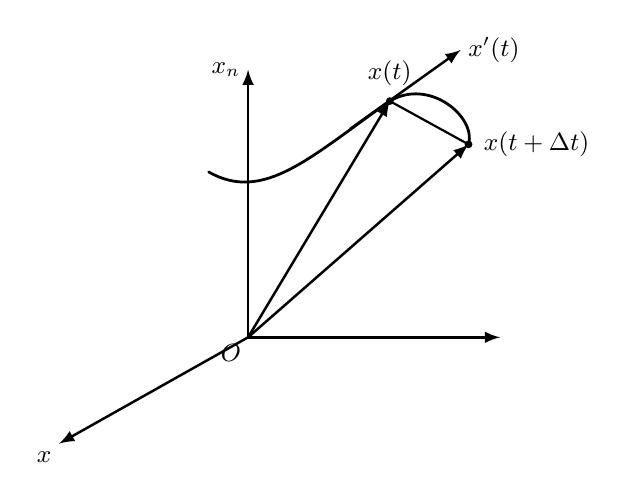
\begin{tikzpicture}[x=1.0cm, y=1.0cm, >=latex, line cap=round, line join=round]
    \draw[line width=0.9pt, ->] (0, 0) -- (-2.4, -1.35) node[below left=-1pt] {\small $x$};
    \draw[line width=0.9pt, ->] (0, 0) -- (3.2, 0);
    \draw[line width=0.9pt, ->] (0, 0) -- (0, 3.4) node[left=-1pt] {\small $x_n$};
    \node[below left=-1pt] at (0, 0) {\small $O$};

    \draw[line width=1.0pt] (-0.5, 2.1) .. controls (0.2, 1.7) and (0.8, 2.3) .. (1.8, 3.0)
                            .. controls (2.3, 3.3) and (2.9, 2.8) .. (2.8, 2.45);

    \coordinate (P) at (1.8, 3.0);
    \coordinate (Q) at (2.8, 2.45);

    \draw[line width=0.9pt, ->] (0, 0) -- (P);
    \draw[line width=0.9pt, ->] (0, 0) -- (Q);
    \draw[line width=0.8pt] (P) -- (Q);

    \draw[line width=0.9pt, ->] (1.3, 2.65) -- (2.7, 3.65) node[right=-1pt] {\small $\boldsymbol{x}'(t)$};

    \fill (P) circle (1.4pt) node[above=2pt] {\small $\boldsymbol{x}(t)$};
    \fill (Q) circle (1.4pt) node[right=2pt] {\small $\boldsymbol{x}(t + \Delta t)$};
  \end{tikzpicture}
  \caption{}\label{fig:9.1.1}
\end{figure}

我们称 $\boldsymbol{x}^{\prime}(t)$ 为曲线 $\boldsymbol{x}(t)$ 在 $t$ 点处的切向量. 当 $t$ 变动时, 得到一个沿曲线 $\boldsymbol{x}(t)$ 的切向量场. 如果 $\boldsymbol{x}(t)$ 为正则曲线, 则 $\dfrac{\boldsymbol{x}^{\prime}(t)}{\|\boldsymbol{x}^{\prime}(t)\|}$ 为沿曲线 $\boldsymbol{x}(t)$ 的单位切向量场. 应该强调的是 $\boldsymbol{x}^{\prime}(t)$ 或 $\dfrac{\boldsymbol{x}^{\prime}(t)}{\|\boldsymbol{x}^{\prime}(t)\|}$ 都是从 $\boldsymbol{x}(t)$ 点出发的向量.

\begin{definition}\label{def:9.1.2}
设 $\boldsymbol{x}(\boldsymbol{u})$ 为 $s$ 维 $C^{k}\,(k \geqslant 1)$ 正则曲面(也记为 $M$), 称 $\boldsymbol{x}'_{u_i}$ 为关于参数坐标 $u_{i}$ 的坐标切向量, 它是 $u_{i}$ 曲线(固定所有参数 $u_{j}\,(j \neq i)$, 只让 $u_{i}$ 变动时的曲线)的切向量. 由于 $\boldsymbol{x}(\boldsymbol{u})$ 为正则曲面, 故 $\operatorname{rank}(\boldsymbol{x}'_{u_1}, \boldsymbol{x}'_{u_2}, \cdots, \boldsymbol{x}'_{u_s}) = s$, 即 $\boldsymbol{x}'_{u_1}, \boldsymbol{x}'_{u_2}, \cdots, \boldsymbol{x}'_{u_s}$ 是线性无关的. 我们称由 $\{\boldsymbol{x}'_{u_1}(\boldsymbol{u}^0), \boldsymbol{x}'_{u_2}(\boldsymbol{u}^0), \cdots, \boldsymbol{x}'_{u_s}(\boldsymbol{u}^0)\}$ 张成的线性子空间
\[
  T_{\boldsymbol{x}(\boldsymbol{u}^{0})}M = \Big\{\sum_{i=1}^{s}\alpha_{i}\boldsymbol{x}_{u_{i}}^{\prime}(\boldsymbol{u}^{0}) \mathrel{\Big|} \alpha_{i} \in \mathbb{R}\Big\}
\]
为曲面 $M$(或 $\boldsymbol{x}(\boldsymbol{u})$)在点 $\boldsymbol{x}(\boldsymbol{u}^{0})$ 处的切空间. $T_{\boldsymbol{x}(\boldsymbol{u}^{0})}M$ 的每个向量称为曲面 $M$ 在点 $\boldsymbol{x}(\boldsymbol{u}^{0})$ 处的切向量. 显然, $T_{\boldsymbol{x}(\boldsymbol{u}^{0})}M$ 为 $s$ 维线性(向量)空间.
\end{definition}

\begin{theorem}\label{thm:9.1.1}
设 $\boldsymbol{x}(\boldsymbol{u})$ 在 $\boldsymbol{u}^{0} \in \Delta$ 处可微, 如果 $\{\boldsymbol{x}_{u_{1}}^{\prime}(\boldsymbol{u}^{0}), \boldsymbol{x}_{u_{2}}^{\prime}(\boldsymbol{u}^{0}), \cdots, \boldsymbol{x}_{u_{s}}^{\prime}(\boldsymbol{u}^{0})\}$ 线性无关, 即 $\operatorname{rank}\{\boldsymbol{x}_{u_{1}}^{\prime}(\boldsymbol{u}^{0}), \boldsymbol{x}_{u_{2}}^{\prime}(\boldsymbol{u}^{0}), \cdots, \boldsymbol{x}_{u_{s}}^{\prime}(\boldsymbol{u}^{0})\} = s$, $\boldsymbol{u}^{0} = \boldsymbol{u}(0)$ 为 $\boldsymbol{u}(t)$ 上一固定点, $\boldsymbol{u}(t)$ 在点 $0$ 处可导, 则
\[
  \frac{\mathrm{d}\boldsymbol{x}(\boldsymbol{u}(t))}{\mathrm{d}t}\bigg|_{t_0} \in T_{\boldsymbol{x}(\boldsymbol{u}^{0})}M,
\]
其中 $M = \boldsymbol{x}(\Delta)$(见\cref{def:9.1.1}).

反之, $\forall \boldsymbol{\alpha} \in \mathbb{R}^{s}$, $\sum_{i=1}^{s} \alpha_{i} \boldsymbol{x}_{u_{i}}^{\prime}(\boldsymbol{u}^{0}) \in T_{\boldsymbol{x}(\boldsymbol{u}^{0})}M$, 必 $\exists \boldsymbol{x}(\boldsymbol{u}(t)) \in M$, s.t. $\boldsymbol{u}(0) = \boldsymbol{u}^{0}$, 且
\[
  \frac{\mathrm{d}\boldsymbol{x}(\boldsymbol{u}(t))}{\mathrm{d}t}\bigg|_{t_0} = \sum_{i=1}^{s}\alpha_{i}\boldsymbol{x}_{u_{i}}^{\prime}(\boldsymbol{u}^{0}).
\]
这表明切空间 $T_{\boldsymbol{x}(\boldsymbol{u}^{0})}M$ 中的任一切向量都可用上述方式得到.
\end{theorem}

\begin{proof}
由于 $\boldsymbol{x}(\boldsymbol{u})$ 在 $\boldsymbol{u}^{0} = \boldsymbol{u}(0)$ 处可微, $\boldsymbol{u}(t)$ 在 $t = 0$ 处可导, 根据定理 8.2.2 与定理 8.2.6 知,
\[
  \frac{\mathrm{d}\boldsymbol{x}(\boldsymbol{u}(t))}{\mathrm{d}t}\bigg|_{t=0} = \sum_{i=1}^{s}\boldsymbol{x}_{u_{i}}^{\prime}(\boldsymbol{u}(0))u_{i}^{\prime}(0) = \sum_{i=1}^{s}u_{i}^{\prime}(0)\boldsymbol{x}_{u_{i}}^{\prime}(\boldsymbol{u}^{0}) \in T_{\boldsymbol{x}(\boldsymbol{u}^{0})}M.
\]
反之, $\forall \boldsymbol{\alpha} \in \mathbb{R}^s$, 令 $\boldsymbol{u}(t) = \boldsymbol{u}^0 + t\boldsymbol{\alpha}$, 则
\[
  \frac{\mathrm{d}\boldsymbol{x}(\boldsymbol{u}^{0} + t\boldsymbol{\alpha})}{\mathrm{d}t}\bigg|_{t=0} = \sum_{i=1}^{s}\alpha_{i}\boldsymbol{x}_{u_{i}}^{\prime}(\boldsymbol{u}^{0}) \in T_{\boldsymbol{x}(\boldsymbol{u}^{0})}M. \qedhere
\]
\end{proof}

曲面 $M$ 在点 $\boldsymbol{x}(\boldsymbol{u}^{0})$ 处的每个切向量 $\sum_{i=1}^{s}\alpha_{i}\boldsymbol{x}_{u_{i}}^{\prime}(\boldsymbol{u}^{0})$ 的起点都为 $\boldsymbol{x}(\boldsymbol{u}^{0})$, 其终点在 $\mathbb{R}^{n}$ 中可表示为(\cref{fig:9.1.2})
\[
  \boldsymbol{y} = \boldsymbol{x}(\boldsymbol{u}^{0}) + \sum_{i=1}^{s}\alpha_{i}\boldsymbol{x}_{u_{i}}^{\prime}(\boldsymbol{u}^{0}).
\]

\begin{figure}[htbp]
  \centering
  \begin{tikzpicture}[x=1.0cm, y=1.0cm, >=latex, line cap=round, line join=round]
    \draw[line width=0.9pt, ->] (0, 0) -- (-1.8, -1.2) node[below left=-1pt] {\small $x_1$};
    \draw[line width=0.9pt, ->] (0, 0) -- (4.0, 0) node[below=-1pt] {\small $x_2$};
    \draw[line width=0.9pt, ->] (0, 0) -- (0, 3.8) node[left=-1pt] {\small $x_3$};
    \node[below left=-1pt] at (0, 0) {\small $O$};

    \draw[line width=1.0pt] (0.8, 2.6) .. controls (1.5, 3.8) and (3.3, 3.6) .. (4.5, 2.8);
    \draw[line width=1.0pt] (0.8, 2.6) .. controls (1.2, 2.1) and (2.0, 2.4) .. (2.6, 2.0)
                            .. controls (3.2, 1.6) and (3.6, 0.9) .. (3.8, 1.0)
                            .. controls (4.0, 1.8) and (4.4, 2.1) .. (4.5, 2.8);
    \node at (4.0, 2.2) {\small $M$};

    \coordinate (X0) at (2.2, 2.6);

    \coordinate (PL1) at (1.8, 2.1);
    \coordinate (PL2) at (4.7, 2.4);
    \coordinate (PL3) at (4.9, 4.3);
    \coordinate (PL4) at (2.0, 4.0);
    \draw[line width=0.9pt] (PL1) -- (PL2) -- (PL3) -- (PL4) -- cycle;

    \draw[line width=0.7pt, dashed] (0, 0) -- ($(0,0)!0.65!(X0)$);
    \draw[line width=0.7pt] ($(0,0)!0.65!(X0)$) -- (X0);

    \draw[line width=1.0pt, ->] (X0) -- ++(1.4, 0.08) node[right=-1pt] {\small $\boldsymbol{x}'_{u_1}(\boldsymbol{u}^0)$};
    \draw[line width=1.0pt, ->] (X0) -- ++(0.15, 1.4) node[above=-1pt] {\small $\boldsymbol{x}'_{u_2}(\boldsymbol{u}^0)$};

    \coordinate (Y) at ($(X0) + (1.2, 1.1)$);
    \draw[line width=0.9pt, ->] (X0) -- (Y);
    \draw[line width=0.7pt, dashed] (0, 0) -- ($(0,0)!0.65!(Y)$);
    \draw[line width=0.7pt] ($(0,0)!0.65!(Y)$) -- (Y);

    \node[anchor=south west, inner sep=1pt] at (3.3, 3.4) {
      \small $\begin{aligned}
        &T_{\boldsymbol{x}(\boldsymbol{u}^0)}M \\
        &\boldsymbol{y} = \boldsymbol{x}(\boldsymbol{u}^0) + \sum_{i=1}^2 \alpha_i \boldsymbol{x}'_{u_i}(\boldsymbol{u}^0)
      \end{aligned}$
    };

    \fill (X0) circle (1.4pt) node[below=2pt] {\small $\boldsymbol{x}(\boldsymbol{u}^0)$};
  \end{tikzpicture}
  \caption{}\label{fig:9.1.2}
\end{figure}

\begin{example}\label{ex:9.1.1}
设 $\boldsymbol{x}\colon (a,b) \to \mathbb{R}^n$ 为 $C^k\,(k \geqslant 1)$ 正则曲线, 记为 $M$. $t_0 \in (a,b)$, 曲线 $\boldsymbol{x}(t)$ 在 $t_0$ 的切向量为 $\boldsymbol{x}'(t_0)$, 切空间 $T_{\boldsymbol{x}(t_0)} M = \{\alpha \boldsymbol{x}'(t_0) \mid \alpha \in \mathbb{R}\}$. 在 $\boldsymbol{x}(t_0)$ 处的切线为 $\boldsymbol{y} = \boldsymbol{x}(t_0) + \alpha \boldsymbol{x}'(t_0)$(向量形式), $\boldsymbol{x}(t_0)$ 为切线上的定点, $\boldsymbol{y}$ 为切线上的动点, $\alpha$ 为切线上的参数(\cref{fig:9.1.3}). 或坐标形式为
\[
  \frac{y_{1} - x_{1}(t_{0})}{x_{1}^{\prime}(t_{0})} = \frac{y_{2} - x_{2}(t_{0})}{x_{2}^{\prime}(t_{0})} = \cdots = \frac{y_{n} - x_{n}(t_{0})}{x_{n}^{\prime}(t_{0})} \, (=\alpha).
\]
\end{example}

\begin{figure}[htbp]
  \centering
  \begin{tikzpicture}[x=1.0cm, y=1.0cm, >=latex, line cap=round, line join=round]
    \draw[line width=0.9pt, ->] (0, 0) -- (-1.8, -1.2) node[below left=-1pt] {\small $x_1$};
    \draw[line width=0.9pt, ->] (0, 0) -- (3.8, 0) node[below=-1pt] {\small $x_2$};
    \draw[line width=0.9pt, ->] (0, 0) -- (0, 3.5) node[left=-1pt] {\small $y$};
    \node[below left=-1pt] at (0, 0) {\small $O$};

    \coordinate (X0) at (1.6, 2.3);

    \coordinate (N1) at (1.2, 3.5);
    \coordinate (N2) at (2.4, 2.7);
    \coordinate (N3) at (2.2, 0.4);
    \coordinate (N4) at (1.0, 1.2);
    \draw[line width=1.1pt] (N1) -- (N2) -- (N3) -- (N4) -- cycle;
    \node at (1.7, 1.4) {\small 法平面};

    \draw[line width=0.9pt] (0.5, 1.4) .. controls (1.1, 1.8) and (1.4, 2.2) .. (X0);
    \draw[line width=0.9pt] (X0) .. controls (1.9, 2.4) and (2.3, 2.7) .. (2.7, 2.6)
                            .. controls (3.1, 2.5) and (3.3, 2.1) .. (3.1, 1.6);
    \node[right=2pt] at (2.6, 2.1) {\small $\boldsymbol{x}(t)$};

    \draw[line width=0.8pt] (0.8, 1.7) -- ($(X0)!0.4!(0.8, 1.7)$);
    \draw[line width=0.8pt, dashed] ($(X0)!0.4!(0.8, 1.7)$) -- (X0);
    \draw[line width=0.8pt, dashed] (X0) -- ($(X0)!0.3!(3.0, 3.2)$);
    \draw[line width=0.9pt, ->] ($(X0)!0.3!(3.0, 3.2)$) -- (3.0, 3.2);
    \node[anchor=west] at (3.0, 3.2) {\small $\boldsymbol{y} = \boldsymbol{x}(t_0) + \alpha \boldsymbol{x}'(t_0)$};

    \draw[line width=0.8pt] (0.5, 2.6) -- (3.0, 1.2);
    \node[below right] at (2.7, 1.3) {\small 割线};

    \draw[line width=0.5pt, ->] (3.8, 3.7) node[right] {\small 切线} -- (3.05, 3.25);
    \draw[line width=0.5pt, ->] (2.2, 3.3) node[above] {\small 切方向} -- (X0);

    \fill (X0) circle (1.4pt) node[above left=-1pt] {\small $\boldsymbol{x}(t_0)$};
  \end{tikzpicture}
  \caption{}\label{fig:9.1.3}
\end{figure}

垂直切向量的超平面
\[
  x_{1}^{\prime}(t_{0})(y_{1} - x_{1}(t_{0})) + x_{2}^{\prime}(t_{0})(y_{2} - x_{2}(t_{0})) + \cdots + x_{n}^{\prime}(t_{0})(y_{n} - x_{n}(t_{0})) = 0
\]
称为曲线 $\boldsymbol{x}(t)$ 在 $\boldsymbol{x}(t_{0})$ 处的法平面. $\boldsymbol{x}(t_{0})$ 为法平面上的定点, 而 $\boldsymbol{y} = (y_{1}, y_{2}, \cdots, y_{n})$ 为法平面上的动点.

\begin{example}\label{ex:9.1.2}
设 $\Delta \subset \mathbb{R}^{2}$ 为开集, $\boldsymbol{x}\colon \Delta \to \mathbb{R}^{3}$, $(u, v) \mapsto \boldsymbol{x}(u, v) = (x(u, v), y(u, v), z(u, v))$ 为 $C^{k}\,(k \geqslant 1)$ 映射, $\operatorname{rank}(\boldsymbol{x}_{u}^{\prime}, \boldsymbol{x}_{v}^{\prime}) = 2$, $M = \boldsymbol{x}(\Delta)$ 为一个二维 $C^{k}$ 正则超曲面, 它的切空间为 $T_{\boldsymbol{x}(u,v)} M = \{\alpha_{1} \boldsymbol{x}_{u}^{\prime}(u, v) + \alpha_{2} \boldsymbol{x}_{v}^{\prime}(u, v) \mid \alpha_{1}, \alpha_{2} \in \mathbb{R}\}$.

在 $\boldsymbol{x}(u,v)$ 处的切超平面为(向量形式)
\[
  \boldsymbol{y} = \boldsymbol{x}(u,v) + \alpha_{1}\boldsymbol{x}_{u}^{\prime}(u,v) + \alpha_{2}\boldsymbol{x}_{v}^{\prime}(u,v).
\]
$\boldsymbol{x}(u,v)$ 为切超平面上的定点, $\boldsymbol{y}$ 为切超平面上的动点, $\alpha_{1}, \alpha_{2}$ 为切超平面上的参数.

与切超平面中从点 $\boldsymbol{x}(u,v)$ 出发的任何切向量 $\alpha_{1}\boldsymbol{x}'_{u}(u,v) + \alpha_{2}\boldsymbol{x}'_{v}(u,v)$ 都正交的向量称为 $\boldsymbol{x}(u,v)$ 点处的法向量. 显然, $\boldsymbol{n}$ 为法向量等价于 $\boldsymbol{n}$ 与 $\boldsymbol{x}'_{u}(u,v)$, $\boldsymbol{x}'_{v}(u,v)$ 都正交.

例如(\cref{fig:9.1.4}),
\begin{align*}
  \boldsymbol{n}(u,v) &= \boldsymbol{x}_{u}^{\prime}(u,v) \times \boldsymbol{x}_{v}^{\prime}(u,v) = \begin{vmatrix}
    \boldsymbol{i} & \boldsymbol{j} & \boldsymbol{k} \\
    \dfrac{\partial x}{\partial u} & \dfrac{\partial y}{\partial u} & \dfrac{\partial z}{\partial u} \\
    \dfrac{\partial x}{\partial v} & \dfrac{\partial y}{\partial v} & \dfrac{\partial z}{\partial v}
  \end{vmatrix} \\
  &= \frac{\partial(y,z)}{\partial(u,v)}\boldsymbol{i} + \frac{\partial(z,x)}{\partial(u,v)}\boldsymbol{j} + \frac{\partial(x,y)}{\partial(u,v)}\boldsymbol{k}
\end{align*}
或等于 $\left(\dfrac{\partial(y,z)}{\partial(u,v)}, \dfrac{\partial(z,x)}{\partial(u,v)}, \dfrac{\partial(x,y)}{\partial(u,v)}\right)$, 它既与 $\boldsymbol{x}_{u}^{\prime}(u,v)$ 正交, 又与 $\boldsymbol{x}_{v}^{\prime}(u,v)$ 正交. 因此, 上述的 $\boldsymbol{n}(u,v)$ 为超曲面 $M$ 在点 $\boldsymbol{x}(u,v)$ 处的法向量. 而切超平面的另一向量形式为
\[
  (\boldsymbol{y} - \boldsymbol{x}(u,v)) \cdot \boldsymbol{n}(u,v) = 0,
\]
其坐标形式为
\[
  \begin{vmatrix}
    y_{1} - x(u,v) & y_{2} - y(u,v) & y_{3} - z(u,v) \\
    \dfrac{\partial x}{\partial u} & \dfrac{\partial y}{\partial u} & \dfrac{\partial z}{\partial u} \\
    \dfrac{\partial x}{\partial v} & \dfrac{\partial y}{\partial v} & \dfrac{\partial z}{\partial v}
  \end{vmatrix} = 0.
\]
\end{example}

\begin{figure}[htbp]
  \centering
  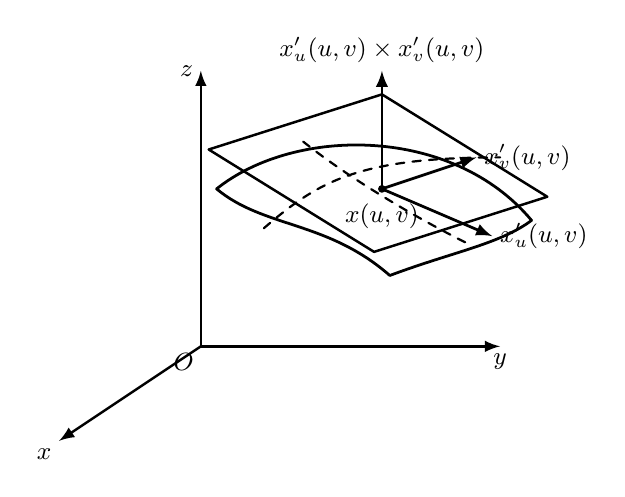
\begin{tikzpicture}[x=1.0cm, y=1.0cm, >=latex, line cap=round, line join=round]
    \draw[line width=0.9pt, ->] (0, 0) -- (-1.8, -1.2) node[below left=-1pt] {\small $x$};
    \draw[line width=0.9pt, ->] (0, 0) -- (3.8, 0) node[below=-1pt] {\small $y$};
    \draw[line width=0.9pt, ->] (0, 0) -- (0, 3.5) node[left=-1pt] {\small $z$};
    \node[below left=-1pt] at (0, 0) {\small $O$};

    \draw[line width=1.0pt] (0.2, 2.0) .. controls (1.2, 2.8) and (3.2, 2.8) .. (4.2, 1.6);
    \draw[line width=1.0pt] (0.2, 2.0) .. controls (0.8, 1.5) and (1.6, 1.6) .. (2.4, 0.9)
                            .. controls (3.2, 1.2) and (3.8, 1.3) .. (4.2, 1.6);

    \coordinate (XUV) at (2.3, 2.0);
    \draw[line width=0.8pt, dashed] (0.8, 1.5) .. controls (1.5, 2.1) and (2.0, 2.4) .. (3.8, 2.4);
    \draw[line width=0.8pt, dashed] (1.3, 2.6) .. controls (1.8, 2.2) and (2.6, 1.7) .. (3.4, 1.3);

    \coordinate (TP1) at (0.1, 2.5);
    \coordinate (TP2) at (2.2, 1.2);
    \coordinate (TP3) at (4.4, 1.9);
    \coordinate (TP4) at (2.3, 3.2);
    \draw[line width=0.9pt] (TP1) -- (TP2) -- (TP3) -- (TP4) -- cycle;

    \draw[line width=1.0pt, ->] (XUV) -- ++(1.4, -0.6) node[right=-1pt] {\small $\boldsymbol{x}'_u(u,v)$};
    \draw[line width=1.0pt, ->] (XUV) -- ++(1.2, 0.4) node[right=-1pt] {\small $\boldsymbol{x}'_v(u,v)$};
    \draw[line width=1.0pt, ->] (XUV) -- ++(0, 1.5) node[above=-1pt] {\small $\boldsymbol{x}'_u(u,v) \times \boldsymbol{x}'_v(u,v)$};

    \fill (XUV) circle (1.4pt) node[below=2pt] {\small $\boldsymbol{x}(u,v)$};
  \end{tikzpicture}
  \caption{}\label{fig:9.1.4}
\end{figure}

$\boldsymbol{n}(u,v)$ 通常不是单位向量. 现在, 我们来计算它的模. 由于
\begin{align*}
  \|\boldsymbol{x}_{u}^{\prime} \times \boldsymbol{x}_{v}^{\prime}\|^{2}
  &= (\|\boldsymbol{x}_{u}^{\prime}\| \|\boldsymbol{x}_{v}^{\prime}\| \sin\theta)^{2} \\
  &= \|\boldsymbol{x}_{u}^{\prime}\|^{2} \|\boldsymbol{x}_{v}^{\prime}\|^{2} (1 - \cos^{2}\theta) \\
  &= \|\boldsymbol{x}_{u}^{\prime}\|^{2} \|\boldsymbol{x}_{v}^{\prime}\|^{2} - (\boldsymbol{x}_{u}^{\prime} \cdot \boldsymbol{x}_{v}^{\prime})^{2} = EG - F^{2} = \det\begin{pmatrix} E & F \\ F & G \end{pmatrix},
\end{align*}
其中
\[
  \left\{\begin{aligned}
    E &= \boldsymbol{x}_{u}^{\prime} \cdot \boldsymbol{x}_{u}^{\prime} = \left(\frac{\partial x}{\partial u}\right)^{2} + \left(\frac{\partial y}{\partial u}\right)^{2} + \left(\frac{\partial z}{\partial u}\right)^{2}, \\
    F &= \boldsymbol{x}_{u}^{\prime} \cdot \boldsymbol{x}_{v}^{\prime} = \frac{\partial x}{\partial u}\frac{\partial x}{\partial v} + \frac{\partial y}{\partial u}\frac{\partial y}{\partial v} + \frac{\partial z}{\partial u}\frac{\partial z}{\partial v}, \\
    G &= \boldsymbol{x}_{v}^{\prime} \cdot \boldsymbol{x}_{v}^{\prime} = \left(\frac{\partial x}{\partial v}\right)^{2} + \left(\frac{\partial y}{\partial v}\right)^{2} + \left(\frac{\partial z}{\partial v}\right)^{2}.
  \end{aligned}\right.
\]
因此, $\boldsymbol{x}(u,v)$ 处的单位法向量为
\[
  \boldsymbol{n}_{0} = \pm\frac{\boldsymbol{x}_{u}^{\prime} \times \boldsymbol{x}_{v}^{\prime}}{\|\boldsymbol{x}_{u}^{\prime} \times \boldsymbol{x}_{v}^{\prime}\|} = \pm\frac{1}{\sqrt{EG - F^{2}}}\left(\frac{\partial(y,z)}{\partial(u,v)}, \frac{\partial(z,x)}{\partial(u,v)}, \frac{\partial(x,y)}{\partial(u,v)}\right).
\]
$E, F, G$ 称为曲面 $M$ 的第一基本量.

设参数 $(u,v)$ 与参数 $(\bar{u},\bar{v})$ 之间存在着一一对应的、一阶连续可导的对应关系
\[
  \left\{\begin{aligned}
    u &= u(\bar{u}, \bar{v}), \\
    v &= v(\bar{u}, \bar{v}),
  \end{aligned}\right. \quad (\bar{u}, \bar{v}) \in \bar{\Delta}, \; (u, v) \in \Delta.
\]
这时曲面 $M$ 有了新的参数表示:
\[
  \boldsymbol{x} = \boldsymbol{x}(u(\bar{u}, \bar{v}), v(\bar{u}, \bar{v})).
\]
直接的计算可知
\begin{align*}
  \bar{\boldsymbol{n}}(\bar{u}, \bar{v}) &= \boldsymbol{x}^{\prime}_{\bar{u}} \times \boldsymbol{x}^{\prime}_{\bar{v}} = \Big(\boldsymbol{x}^{\prime}_{u}\frac{\partial u}{\partial\bar{u}} + \boldsymbol{x}^{\prime}_{v}\frac{\partial v}{\partial\bar{u}}\Big) \times \Big(\boldsymbol{x}^{\prime}_{u}\frac{\partial u}{\partial\bar{v}} + \boldsymbol{x}^{\prime}_{v}\frac{\partial v}{\partial\bar{v}}\Big) \\
  &= \Big(\frac{\partial u}{\partial\bar{u}}\frac{\partial v}{\partial\bar{v}} - \frac{\partial u}{\partial\bar{v}}\frac{\partial v}{\partial\bar{u}}\Big)\boldsymbol{x}^{\prime}_{u} \times \boldsymbol{x}^{\prime}_{v} \\
  &= \frac{\partial(u,v)}{\partial(\bar{u},\bar{v})}\boldsymbol{x}^{\prime}_{u} \times \boldsymbol{x}^{\prime}_{v} = \frac{\partial(u,v)}{\partial(\bar{u},\bar{v})}\boldsymbol{n}(u,v).
\end{align*}
注意, 由于
\[
  1 = \frac{\partial(u,v)}{\partial(u,v)} = \frac{\partial(u,v)}{\partial(\bar{u},\bar{v})}\frac{\partial(\bar{u},\bar{v})}{\partial(u,v)},
\]
故
\[
  \frac{\partial(u,v)}{\partial(\bar{u},\bar{v})} \neq 0, \quad \frac{\partial(\bar{u},\bar{v})}{\partial(u,v)} \neq 0.
\]
如果 $\dfrac{\partial(u,v)}{\partial(\bar{u},\bar{v})} > 0\,(< 0)$, 则 $\bar{\boldsymbol{n}}(\bar{u},\bar{v})$ 与 $\boldsymbol{n}(u,v)$ 同(反)向, 我们称 $(\bar{u},\bar{v})$ 与 $(u,v)$ 为同(反)向的参数.

更一般地, 我们有下面结果.

\begin{example}\label{ex:9.1.3}
设 $\Delta \subset \mathbb{R}^{n-1}$ 为开集,
\[
  \boldsymbol{x}\colon \Delta \to \mathbb{R}^{n}, \quad \boldsymbol{u} = (u_{1}, u_{2}, \cdots, u_{n-1}) \mapsto \boldsymbol{x}(\boldsymbol{u}) = (x_{1}(\boldsymbol{u}), x_{2}(\boldsymbol{u}), \cdots, x_{n}(\boldsymbol{u}))
\]
为 $C^{k}\,(k \geqslant 1)$ 映射, $\operatorname{rank}(\boldsymbol{x}_{u_{1}}^{\prime}, \boldsymbol{x}_{u_{2}}^{\prime}, \cdots, \boldsymbol{x}_{u_{n-1}}^{\prime}) = n - 1$, $M = \boldsymbol{x}(\Delta)$ 为一个 $n - 1$ 维 $C^{k}$ 正则超曲面, 它的切空间为
\[
  T_{\boldsymbol{x}(\boldsymbol{u})}M = \Big\{\sum_{i=1}^{n-1}\alpha_{i}\boldsymbol{x}_{u_{i}}^{\prime}(\boldsymbol{u}) \mathrel{\Big|} \alpha_{i} \in \mathbb{R}, \, i = 1, 2, \cdots, n - 1\Big\}.
\]
在 $\boldsymbol{x}(\boldsymbol{u})$ 处的切超平面为(向量形式)
\[
  \boldsymbol{y} = \boldsymbol{x}(\boldsymbol{u}) + \sum_{i=1}^{n-1}\alpha_{i}\boldsymbol{x}_{u_{i}}^{\prime}(\boldsymbol{u}).
\]
$\boldsymbol{x}(\boldsymbol{u})$ 为切超平面上的定点, $\boldsymbol{y}$ 为切超平面上的动点, $\alpha_{1}, \alpha_{2}, \cdots, \alpha_{n-1}$ 为切超平面上的参数.

与切超平面中从点 $\boldsymbol{x}(\boldsymbol{u})$ 出发的任何切向量 $\sum_{i=1}^{n-1}\alpha_i \boldsymbol{x}'_{u_i}(\boldsymbol{u})$ 都正交的向量称为 $\boldsymbol{x}(\boldsymbol{u})$ 点处的法向量. 显然,
\[
  \boldsymbol{n} \text{ 为法向量} \iff \boldsymbol{n} \text{ 与每个 } \boldsymbol{x}'_{u_i}\,(i = 1, 2, \cdots, n - 1) \text{ 都正交}.
\]
例如, 设 $\{\boldsymbol{e}_{1}, \boldsymbol{e}_{2}, \cdots, \boldsymbol{e}_{n}\}$ 为 $\mathbb{R}^{n}$ 中的规范正交基(当 $n = 3$ 时, $\boldsymbol{e}_{1} = \boldsymbol{i}$, $\boldsymbol{e}_{2} = \boldsymbol{j}$, $\boldsymbol{e}_{3} = \boldsymbol{k}$), 则
\[
  \boldsymbol{n}(\boldsymbol{u}) = \begin{vmatrix}
    \boldsymbol{e}_{1} & \cdots & \boldsymbol{e}_{n} \\
    \dfrac{\partial x_{1}}{\partial u_{1}} & \cdots & \dfrac{\partial x_{n}}{\partial u_{1}} \\
    \vdots & & \vdots \\
    \dfrac{\partial x_{1}}{\partial u_{n-1}} & \cdots & \dfrac{\partial x_{n}}{\partial u_{n-1}}
  \end{vmatrix} = \sum_{i=1}^{n}(-1)^{1+i}\frac{\partial(x_{1}, x_{2}, \cdots, \hat{x}_{i}, \cdots, x_{n})}{\partial(u_{1}, u_{2}, \cdots, u_{n-1})}\boldsymbol{e}_{i}
\]
与每个 $\dfrac{\partial\boldsymbol{x}}{\partial u_{i}}$ 正交 $(i = 1, 2, \cdots, n - 1)$, 其中 $\hat{x}_{i}$ 表示删去 $x_{i}$. 换言之,
\[
  \boldsymbol{n}(\boldsymbol{u}) \cdot \frac{\partial\boldsymbol{x}}{\partial u_{i}} = \begin{vmatrix}
    \dfrac{\partial x_{1}}{\partial u_{i}} & \cdots & \dfrac{\partial x_{n}}{\partial u_{i}} \\
    \dfrac{\partial x_{1}}{\partial u_{1}} & \cdots & \dfrac{\partial x_{n}}{\partial u_{1}} \\
    \vdots & & \vdots \\
    \dfrac{\partial x_{1}}{\partial u_{n-1}} & \cdots & \dfrac{\partial x_{n}}{\partial u_{n-1}}
  \end{vmatrix} = 0.
\]
因此, 上述的 $\boldsymbol{n}(\boldsymbol{u})$ 为超曲面 $M$ 在点 $\boldsymbol{x}(\boldsymbol{u})$ 处的法向量, 而切超平面的另一向量形式为
\[
  (\boldsymbol{y} - \boldsymbol{x}(\boldsymbol{u})) \cdot \boldsymbol{n}(\boldsymbol{u}) = 0,
\]
其坐标形式为
\[
  \begin{vmatrix}
    y_{1} - x_{1}(\boldsymbol{u}) & \cdots & y_{n} - x_{n}(\boldsymbol{u}) \\
    \dfrac{\partial x_{1}}{\partial u_{1}} & \cdots & \dfrac{\partial x_{n}}{\partial u_{1}} \\
    \vdots & & \vdots \\
    \dfrac{\partial x_{1}}{\partial u_{n-1}} & \cdots & \dfrac{\partial x_{n}}{\partial u_{n-1}}
  \end{vmatrix} = 0.
\]
$\boldsymbol{n}(\boldsymbol{u})$ 通常不是单位向量. 当 $n \neq 3$ 时, 不能用 $\|\boldsymbol{x}'_{u} \times \boldsymbol{x}'_{v}\|$ 的方法来求 $\boldsymbol{n}(\boldsymbol{u})$ 的模. 但由其结果 $\|\boldsymbol{x}_{u}^{\prime} \times \boldsymbol{x}_{v}^{\prime}\|^{2} = \det\begin{pmatrix} E & F \\ F & G \end{pmatrix}$ 的启发, 我们有如下推导:

设 $g_{ij} = \boldsymbol{x}'_{u_i} \cdot \boldsymbol{x}'_{u_j} = \sum_{l=1}^{n} \dfrac{\partial x_l}{\partial u_i}\dfrac{\partial x_l}{\partial u_j}$, $i, j = 1, 2, \cdots, n - 1$. 则
\begin{align*}
  \|\boldsymbol{n}(\boldsymbol{u})\| &= \boldsymbol{n}(\boldsymbol{u}) \cdot \boldsymbol{n}_{0}(\boldsymbol{u}) = \begin{vmatrix}
    \boldsymbol{e}_{1} & \cdots & \boldsymbol{e}_{n} \\
    \dfrac{\partial x_{1}}{\partial u_{1}} & \cdots & \dfrac{\partial x_{n}}{\partial u_{1}} \\
    \vdots & & \vdots \\
    \dfrac{\partial x_{1}}{\partial u_{n-1}} & \cdots & \dfrac{\partial x_{n}}{\partial u_{n-1}}
  \end{vmatrix} \cdot \sum_{i=1}^{n}h_{i}\boldsymbol{e}_{i} \\
  &= \begin{vmatrix}
    h_{1} & \cdots & h_{n} \\
    \dfrac{\partial x_{1}}{\partial u_{1}} & \cdots & \dfrac{\partial x_{n}}{\partial u_{1}} \\
    \vdots & & \vdots \\
    \dfrac{\partial x_{1}}{\partial u_{n-1}} & \cdots & \dfrac{\partial x_{n}}{\partial u_{n-1}}
  \end{vmatrix} \\
  &= \sqrt{\det\begin{pmatrix}
    h_{1} & \cdots & h_{n} \\
    \dfrac{\partial x_{1}}{\partial u_{1}} & \cdots & \dfrac{\partial x_{n}}{\partial u_{1}} \\
    \vdots & & \vdots \\
    \dfrac{\partial x_{1}}{\partial u_{n-1}} & \cdots & \dfrac{\partial x_{n}}{\partial u_{n-1}}
  \end{pmatrix}\begin{pmatrix}
    h_{1} & \dfrac{\partial x_{1}}{\partial u_{1}} & \cdots & \dfrac{\partial x_{1}}{\partial u_{n-1}} \\
    \vdots & \vdots & & \vdots \\
    h_{n} & \dfrac{\partial x_{n}}{\partial u_{1}} & \cdots & \dfrac{\partial x_{n}}{\partial u_{n-1}}
  \end{pmatrix}} \\
  &= \sqrt{\det\begin{pmatrix}
    1 & 0 & \cdots & 0 \\
    0 & g_{11} & \cdots & g_{1,n-1} \\
    \vdots & \vdots & & \vdots \\
    0 & g_{n-1,1} & \cdots & g_{n-1,n-1}
  \end{pmatrix}} \\
  &= \sqrt{\det\begin{pmatrix}
    g_{11} & \cdots & g_{1,n-1} \\
    \vdots & & \vdots \\
    g_{n-1,1} & \cdots & g_{n-1,n-1}
  \end{pmatrix}} = \sqrt{\det(g_{ij})},
\end{align*}
其中 $\sum_{i=1}^{n}h_{i}\boldsymbol{e}_{i} = \boldsymbol{n}_{0}(\boldsymbol{u})$ 为与 $\boldsymbol{n}(\boldsymbol{u})$ 同方向的单位法向量. 因此, $\boldsymbol{x}(\boldsymbol{u})$ 处的单位法向量为
\[
  \boldsymbol{n}_{0}(\boldsymbol{u}) = \pm\frac{\boldsymbol{n}(\boldsymbol{u})}{\|\boldsymbol{n}(\boldsymbol{u})\|} = \pm\frac{1}{\sqrt{\det(g_{ij})}}\sum_{i=1}^{n}(-1)^{1+i}\frac{\partial(x_{1}, x_{2}, \cdots, \hat{x}_{i}, \cdots, x_{n})}{\partial(u_{1}, u_{2}, \cdots, u_{n-1})}\boldsymbol{e}_{i}.
\]
$g_{ij}\,(i, j = 1, 2, \cdots, n - 1)$ 称为超曲面 $M$ 的第一基本量. 当 $n = 3$ 时, $g_{11} = E$, $g_{12} = g_{21} = F$, $g_{22} = G$.

设参数 $(u_{1}, u_{2}, \cdots, u_{n-1})$ 与参数 $(\bar{u}_{1}, \bar{u}_{2}, \cdots, \bar{u}_{n-1})$ 之间存在着一一对应的、一阶连续可导的对应关系
\[
  \left\{\begin{aligned}
    u_{1} &= u_{1}(\bar{u}_{1}, \bar{u}_{2}, \cdots, \bar{u}_{n-1}), \\
    &\;\;\vdots \\
    u_{n-1} &= u_{n-1}(\bar{u}_{1}, \bar{u}_{2}, \cdots, \bar{u}_{n-1}),
  \end{aligned}\right. \quad \bar{\boldsymbol{u}} = (\bar{u}_{1}, \bar{u}_{2}, \cdots, \bar{u}_{n-1}) \in \bar{\Delta}, \; \boldsymbol{u} = (u_{1}, u_{2}, \cdots, u_{n-1}) \in \Delta.
\]
这时曲面 $M$ 有了新的参数表示:
\[
  \boldsymbol{x} = \boldsymbol{x}(\boldsymbol{u}(\bar{\boldsymbol{u}})) = \boldsymbol{x}(u_{1}(\bar{u}_{1}, \cdots, \bar{u}_{n-1}), u_{2}(\bar{u}_{1}, \cdots, \bar{u}_{n-1}), \cdots, u_{n-1}(\bar{u}_{1}, \cdots, \bar{u}_{n-1})).
\]
直接计算可知
\begin{align*}
  \bar{\boldsymbol{n}}(\bar{\boldsymbol{u}}) &= \begin{vmatrix}
    \boldsymbol{e}_{1} & \cdots & \boldsymbol{e}_{n} \\
    \dfrac{\partial x_{1}}{\partial\bar{u}_{1}} & \cdots & \dfrac{\partial x_{n}}{\partial\bar{u}_{1}} \\
    \vdots & & \vdots \\
    \dfrac{\partial x_{1}}{\partial\bar{u}_{n-1}} & \cdots & \dfrac{\partial x_{n}}{\partial\bar{u}_{n-1}}
  \end{vmatrix} = \sum_{i=1}^{n}(-1)^{1+i}\frac{\partial(x_{1}, x_{2}, \cdots, \hat{x}_{i}, \cdots, x_{n})}{\partial(\bar{u}_{1}, \bar{u}_{2}, \cdots, \bar{u}_{n-1})}\boldsymbol{e}_{i} \\
  &= \sum_{i=1}^{n}(-1)^{1+i}\frac{\partial(x_{1}, x_{2}, \cdots, \hat{x}_{i}, \cdots, x_{n})}{\partial(u_{1}, u_{2}, \cdots, u_{n-1})}\frac{\partial(u_{1}, u_{2}, \cdots, u_{n-1})}{\partial(\bar{u}_{1}, \bar{u}_{2}, \cdots, \bar{u}_{n-1})}\boldsymbol{e}_{i} \\
  &= \frac{\partial(u_{1}, u_{2}, \cdots, u_{n-1})}{\partial(\bar{u}_{1}, \bar{u}_{2}, \cdots, \bar{u}_{n-1})}\boldsymbol{n}(\boldsymbol{u}).
\end{align*}
\end{example}

注意, 由于
\[
  1 = \frac{\partial(u_{1}, u_{2}, \cdots, u_{n-1})}{\partial(u_{1}, u_{2}, \cdots, u_{n-1})} = \frac{\partial(u_{1}, u_{2}, \cdots, u_{n-1})}{\partial(\bar{u}_{1}, \bar{u}_{2}, \cdots, \bar{u}_{n-1})}\frac{\partial(\bar{u}_{1}, \bar{u}_{2}, \cdots, \bar{u}_{n-1})}{\partial(u_{1}, u_{2}, \cdots, u_{n-1})},
\]
故
\[
  \frac{\partial(u_{1}, u_{2}, \cdots, u_{n-1})}{\partial(\bar{u}_{1}, \bar{u}_{2}, \cdots, \bar{u}_{n-1})} \neq 0, \quad \frac{\partial(\bar{u}_{1}, \bar{u}_{2}, \cdots, \bar{u}_{n-1})}{\partial(u_{1}, u_{2}, \cdots, u_{n-1})} \neq 0.
\]
如果 $\dfrac{\partial(u_{1}, u_{2}, \cdots, u_{n-1})}{\partial(\bar{u}_{1}, \bar{u}_{2}, \cdots, \bar{u}_{n-1})} > 0\,(< 0)$, 则 $\bar{\boldsymbol{n}}(\bar{\boldsymbol{u}})$ 与 $\boldsymbol{n}(\boldsymbol{u})$ 同(反)向, 我们称 $(\bar{u}_{1}, \bar{u}_{2}, \cdots, \bar{u}_{n-1})$ 与 $(u_{1}, u_{2}, \cdots, u_{n-1})$ 为同(反)向的参数.

上面已详细讨论了 $C^{k}\,(k \geqslant 1)$ 正则超曲面的切空间, 法向量. 自然会问: $s$ 维 $C^{k}\,(k \geqslant 1)$ 的正则曲面的法空间应如何表示? 我们期望能用切空间 $T_{\boldsymbol{x}(\boldsymbol{u})}M$ 的基 $\{\boldsymbol{x}_{u_1}^{\prime}(\boldsymbol{u}),\allowbreak \boldsymbol{x}_{u_2}^{\prime}(\boldsymbol{u}),\allowbreak \cdots,\allowbreak \boldsymbol{x}_{u_s}^{\prime}(\boldsymbol{u})\}$ 来表达法空间
\[
  T_{\boldsymbol{x}(\boldsymbol{u})}^{\perp}M = \left\{\boldsymbol{n} \mathrel{\Big|} \boldsymbol{n} \perp T_{\boldsymbol{x}(\boldsymbol{u})}M, \text{ 即 } \boldsymbol{n} \cdot \boldsymbol{x}^{\prime}_{u_{i}}(\boldsymbol{u}) = 0, \, i = 1, 2, \cdots, s\right\},
\]
或者来表达法空间的一个基.

\begin{example}\label{ex:9.1.4}
设 $\boldsymbol{x}(\boldsymbol{u})$ 为 $s$ 维 $C^{k}\,(k \geqslant 1)$ 正则曲面, 则
\[
  (\boldsymbol{P} \quad \boldsymbol{Q}) = \begin{pmatrix}
    \dfrac{\partial\boldsymbol{x}(\boldsymbol{u})}{\partial u_{1}} \\
    \vdots \\
    \dfrac{\partial\boldsymbol{x}(\boldsymbol{u})}{\partial u_{s}}
  \end{pmatrix} = \begin{pmatrix}
    \dfrac{\partial x_{1}}{\partial u_{1}} & \cdots & \dfrac{\partial x_{n}}{\partial u_{1}} \\
    \vdots & & \vdots \\
    \dfrac{\partial x_{1}}{\partial u_{s}} & \cdots & \dfrac{\partial x_{n}}{\partial u_{s}}
  \end{pmatrix}.
\]
由于 $\operatorname{rank}(\boldsymbol{P} \quad \boldsymbol{Q}) = s$, 为叙述简单起见, 不妨设
\[
  \boldsymbol{P} = \begin{pmatrix}
    \dfrac{\partial x_{1}}{\partial u_{1}} & \cdots & \dfrac{\partial x_{s}}{\partial u_{1}} \\
    \vdots & & \vdots \\
    \dfrac{\partial x_{1}}{\partial u_{s}} & \cdots & \dfrac{\partial x_{s}}{\partial u_{s}}
  \end{pmatrix}
\]
为 $s \times s$ 非异矩阵. 因为
\begin{align*}
  (\boldsymbol{P} \quad \boldsymbol{Q})\left(-(\boldsymbol{P}^{-1}\boldsymbol{Q})^{\mathrm{T}} \quad \boldsymbol{I}_{n-s}\right)^{\mathrm{T}}
  &= (\boldsymbol{P} \quad \boldsymbol{Q})\begin{pmatrix} -\boldsymbol{P}^{-1}\boldsymbol{Q} \\ \boldsymbol{I}_{n-s} \end{pmatrix} \\
  &= -\boldsymbol{P}(\boldsymbol{P}^{-1}\boldsymbol{Q}) + \boldsymbol{Q}\boldsymbol{I}_{n-s} = -\boldsymbol{Q} + \boldsymbol{Q} = \boldsymbol{0},
\end{align*}
所以, $(\boldsymbol{P} \quad \boldsymbol{Q})$ 的行向量都正交于 $\left(-(\boldsymbol{P}^{-1}\boldsymbol{Q})^{\mathrm{T}} \quad \boldsymbol{I}_{n-s}\right)$ 的行向量. 此外, 显然有
\[
  \operatorname{rank}\left(-(\boldsymbol{P}^{-1}\boldsymbol{Q})^{\mathrm{T}} \quad \boldsymbol{I}_{n-s}\right) = n - s.
\]
因此, $\left(-(\boldsymbol{P}^{-1}\boldsymbol{Q})^{\mathrm{T}} \quad \boldsymbol{I}_{n-s}\right)$ 的 $n - s$ 个行向量为法空间 $T_{\boldsymbol{x}(\boldsymbol{u})}^{\perp}M$ 的一个基, 它由 $(\boldsymbol{P} \quad \boldsymbol{Q})$ 的元素所表达, 即由 $\dfrac{\partial x_{i}}{\partial u_{j}}\,(i = 1, 2, \cdots, n; \, j = 1, 2, \cdots, s)$ 所完全表达.
\end{example}

上述简洁的论述是难以想到的, 这是在查阅 Grassmann 流形 $G_{n-s,s}$ 与 $G_{s,n-s}$ 之间是微分同胚时, 见到的推导.

\begin{example}\label{ex:9.1.5}
设 $U \subset \mathbb{R}^n$ 为开集, $f\colon U \to \mathbb{R}^1$ 为 $C^k\,(1 \leqslant k \leqslant +\infty)$ 映射, 且在 $U$ 上,
\[
  \operatorname{rank} f = \operatorname{rank} \boldsymbol{J}f = \operatorname{rank}\left(\frac{\partial f}{\partial x_{1}}, \frac{\partial f}{\partial x_{2}}, \cdots, \frac{\partial f}{\partial x_{n}}\right) \equiv 1 \text{ (常值)},
\]
由例 8.4.5 知
\[
  M = f^{-1}(q) = \{\boldsymbol{x} \in U \mid f(\boldsymbol{x}) = q\} = \{\boldsymbol{x} \in U \mid f(\boldsymbol{x}) - q = 0\}
\]
{\emergencystretch=3em 或为空集, 或为 $n - 1$ 维 $C^{k}$ 流形或 $C^{k}$ 超曲面. 证明: 当 $M \neq \varnothing$ 时, $\operatorname{grad}f = \left(\dfrac{\partial f}{\partial x_{1}},\allowbreak \dfrac{\partial f}{\partial x_{2}},\allowbreak \cdots,\allowbreak \dfrac{\partial f}{\partial x_{n}}\right)$ 为 $M$ 的法向量场. 从而, 过定点 $\boldsymbol{x}^{0} \in M$ 的切超平面为\par}
\[
  (\boldsymbol{y} - \boldsymbol{x}^{0}) \cdot \operatorname{grad}f(\boldsymbol{x}^{0}) = 0,
\]
即
\[
  \sum_{i=1}^{n}\frac{\partial f}{\partial x_{i}}(\boldsymbol{x}^{0})(y_{i} - x_{i}^{0}) = 0.
\]
\end{example}

\begin{proof}[证法 1]
设 $M \neq \varnothing$, $\boldsymbol{x}(t)$ 为 $M$ 上过定点 $\boldsymbol{x}^{0} = \boldsymbol{x}(0)$ 的任一 $C^{1}$ 曲线, 则
\[
  f(\boldsymbol{x}(t)) \equiv q,
\]
两边对 $t$ 求导得到
\[
  \operatorname{grad}f \cdot \frac{\mathrm{d}\boldsymbol{x}}{\mathrm{d}t} = \sum_{i=1}^{n}\frac{\partial f}{\partial x_{i}}(\boldsymbol{x}(t))\frac{\mathrm{d}x_{i}}{\mathrm{d}t} \equiv 0,
\]
它表明 $f$ 的梯度向量 $\operatorname{grad}f \equiv \left(\dfrac{\partial f}{\partial x_{1}}, \dfrac{\partial f}{\partial x_{2}}, \cdots, \dfrac{\partial f}{\partial x_{n}}\right)\bigg|_{\boldsymbol{x}^{0}}$ 与曲面 $M$ 上点 $\boldsymbol{x}^{0}$ 处的切向量 $\boldsymbol{x}^{\prime}(0)$ 正交. 由于 $\boldsymbol{x}(t)$ 的任意性, $\operatorname{grad}f = \left(\dfrac{\partial f}{\partial x_{1}}, \dfrac{\partial f}{\partial x_{2}}, \cdots, \dfrac{\partial f}{\partial x_{n}}\right)\bigg|_{\boldsymbol{x}^{0}}$ 为 $T_{\boldsymbol{x}^{0}}M$ 的法向量.
\end{proof}

\begin{proof}[证法 2]
设 $M \neq \varnothing$, 不妨令 $\dfrac{\partial f}{\partial x_{n}} \neq 0$, 根据隐函数定理, 在局部, $x_{n} = x_{n}(x_{1}, x_{2}, \cdots, x_{n-1})$, 且
\[
  \frac{\partial x_{n}}{\partial x_{i}} = -\frac{\dfrac{\partial f}{\partial x_{i}}}{\dfrac{\partial f}{\partial x_{n}}}.
\]
由于局部参数表示为 $\boldsymbol{x} = \boldsymbol{x}(x_{1}, x_{2}, \cdots, x_{n-1}) = (x_{1}, x_{2}, \cdots, x_{n-1}, x_{n}(x_{1}, \cdots, x_{n-1}))$, 故
\[
  \left\{\begin{aligned}
    \boldsymbol{x}_{u_{1}}^{\prime} &= \left(1, 0, \cdots, 0, -\frac{\dfrac{\partial f}{\partial x_{1}}}{\dfrac{\partial f}{\partial x_{n}}}\right), \\
    &\;\;\vdots \\
    \boldsymbol{x}_{u_{n-1}}^{\prime} &= \left(0, 0, \cdots, 1, -\frac{\dfrac{\partial f}{\partial x_{n-1}}}{\dfrac{\partial f}{\partial x_{n}}}\right).
  \end{aligned}\right.
\]
显然,
\[
  \operatorname{grad}f \cdot \boldsymbol{x}_{u_{i}}^{\prime} = \left(\frac{\partial f}{\partial x_{1}}, \frac{\partial f}{\partial x_{2}}, \cdots, \frac{\partial f}{\partial x_{n}}\right) \cdot \left(0, \cdots, 0, \underset{\text{第 } i \text{ 个}}{1}, 0, \cdots, -\frac{\dfrac{\partial f}{\partial x_{i}}}{\dfrac{\partial f}{\partial x_{n}}}\right) = 0.
\]
因此, $\operatorname{grad}f = \left(\dfrac{\partial f}{\partial x_{1}}, \dfrac{\partial f}{\partial x_{2}}, \cdots, \dfrac{\partial f}{\partial x_{n}}\right)$ 为 $T_{\boldsymbol{x}(x_{1}, x_{2}, \cdots, x_{n-1})}M$ 的法向量. \qedhere
\end{proof}

\begin{definition}\label{def:9.1.3}
设 $\Delta_{i} \subset \mathbb{R}^{s_{i}}$ 为开集, $\varphi_{i}^{-1}\colon \Delta_{i} \to \varphi_{i}^{-1}(\Delta_{i}) \subset \mathbb{R}^{n_{i}}$ 为同胚, $i = 1, 2$, $\varphi_{1}^{-1}(\boldsymbol{u}) = \boldsymbol{x}(\boldsymbol{u})$ 为 $s_{1}$ 维 $C^{k}\,(k \geqslant 1)$ 正则曲面 $M_{1}$, $\varphi_{2}^{-1}(\boldsymbol{v}) = \boldsymbol{y}(\boldsymbol{v})$ 为 $s_{2}$ 维 $C^{k}$ 正则曲面 $M_{2}$. $\boldsymbol{u}(t)$ 为 $M_{1}$ 上的一条 $C^{1}$ 曲线. 如果映射 $f\colon M_{1} \to M_{2}$ 是 $C^{k}$ 的, 即 $\varphi_{2} \circ f \circ \varphi_{1}^{-1}\colon \Delta_{1} \to \Delta_{2}$ 为 $C^{k}$ 映射, 也就是分量
\[
  \left\{\begin{aligned}
    v_{1} &= (\varphi_{2} \circ f \circ \varphi_{1}^{-1})_{1}(u_{1}, u_{2}, \cdots, u_{s_{1}}), \\
    &\;\;\vdots \\
    v_{s_{2}} &= (\varphi_{2} \circ f \circ \varphi_{1}^{-1})_{s_{2}}(u_{1}, u_{2}, \cdots, u_{s_{1}})
  \end{aligned}\right.
\]
为 $C^{k}$ 的函数, 于是, $\boldsymbol{y} = \boldsymbol{y}(\boldsymbol{v}(\boldsymbol{u}(t))) = \boldsymbol{y}(\varphi_{2} \circ f \circ \varphi_{1}^{-1})(\boldsymbol{u}(t))$ 为 $M_{2}$ 上一条 $C^{1}$ 曲线. 易见,
\[
  f_{*}\left(\frac{\mathrm{d}\boldsymbol{x}}{\mathrm{d}t}\right) = \frac{\mathrm{d}\boldsymbol{y}}{\mathrm{d}t} = \sum_{j=1}^{s_{2}}\frac{\partial\boldsymbol{y}}{\partial v_{j}}\frac{\mathrm{d}v_{j}}{\mathrm{d}t} = \sum_{j=1}^{s_{2}}\frac{\partial\boldsymbol{y}}{\partial v_{j}}\sum_{i=1}^{s_{1}}\frac{\partial v_{j}}{\partial u_{i}}\frac{\mathrm{d}u_{i}}{\mathrm{d}t},
\]
\[
  \begin{pmatrix}
    \dfrac{\mathrm{d}v_{1}}{\mathrm{d}t} \\
    \vdots \\
    \dfrac{\mathrm{d}v_{s_{2}}}{\mathrm{d}t}
  \end{pmatrix} = \begin{pmatrix}
    \dfrac{\partial v_{1}}{\partial u_{1}} & \cdots & \dfrac{\partial v_{1}}{\partial u_{s_{1}}} \\
    \vdots & & \vdots \\
    \dfrac{\partial v_{s_{2}}}{\partial u_{1}} & \cdots & \dfrac{\partial v_{s_{2}}}{\partial u_{s_{1}}}
  \end{pmatrix}\begin{pmatrix}
    \dfrac{\mathrm{d}u_{1}}{\mathrm{d}t} \\
    \vdots \\
    \dfrac{\mathrm{d}u_{s_{1}}}{\mathrm{d}t}
  \end{pmatrix}.
\]
特别地, 当 $t = u_{i}$ 时,
\[
  f_{*}\left(\frac{\partial\boldsymbol{x}}{\partial u_{i}}\right) = \sum_{j=1}^{s_{2}}\frac{\partial\boldsymbol{y}}{\partial v_{j}}\frac{\partial v_{j}}{\partial u_{i}}.
\]
因此,
\[
  \begin{pmatrix}
    f_{*}\left(\dfrac{\partial\boldsymbol{x}}{\partial u_{1}}\right) \\
    \vdots \\
    f_{*}\left(\dfrac{\partial\boldsymbol{x}}{\partial u_{s_{1}}}\right)
  \end{pmatrix} = \begin{pmatrix}
    \dfrac{\partial v_{1}}{\partial u_{1}} & \cdots & \dfrac{\partial v_{s_{2}}}{\partial u_{1}} \\
    \vdots & & \vdots \\
    \dfrac{\partial v_{1}}{\partial u_{s_{1}}} & \cdots & \dfrac{\partial v_{s_{2}}}{\partial u_{s_{1}}}
  \end{pmatrix}\begin{pmatrix}
    \dfrac{\partial\boldsymbol{y}}{\partial v_{1}} \\
    \vdots \\
    \dfrac{\partial\boldsymbol{y}}{\partial v_{s_{2}}}
  \end{pmatrix}.
\]
显然, 上式决定了一个线性映射 $f_{*\boldsymbol{x}(\boldsymbol{u})}\colon T_{\boldsymbol{x}(\boldsymbol{u})}M_{1} \to T_{f(\boldsymbol{x}(\boldsymbol{u}))}M_{2}$(\cref{fig:9.1.5}), 称为切映射或 Jacobi 映射或 $f$ 的微分. 有时记 $f_{*\boldsymbol{x}(\boldsymbol{u})} = \mathrm{d}f(\boldsymbol{x}(\boldsymbol{u}))$.
\end{definition}

\begin{figure}[htbp]
  \centering
  \begin{tikzpicture}[x=0.95cm, y=0.95cm, >=latex, line cap=round, line join=round]
    \draw[line width=1.0pt] (-4.5, 2.8) .. controls (-3.0, 3.8) and (-1.8, 3.6) .. (-0.6, 2.7);
    \draw[line width=1.0pt] (-4.5, 2.8) .. controls (-3.5, 2.7) and (-2.5, 2.8) .. (-1.8, 1.7)
                            .. controls (-1.3, 2.2) and (-0.9, 2.5) .. (-0.6, 2.7);
    \node at (-2.0, 2.3) {\small $M_1$};
    \draw[line width=0.9pt] (-3.4, 2.9) .. controls (-2.8, 3.4) and (-2.0, 3.5) .. (-1.4, 3.3);
    \coordinate (XM1) at (-2.4, 3.35);
    \fill (XM1) circle (1.3pt) node[below=2pt] {\small $\boldsymbol{x}(\boldsymbol{u}(t))$};
    \draw[line width=0.9pt, ->] (XM1) -- ++(-0.9, 0.45) node[above=-1pt] {\small $\dfrac{\mathrm{d}\boldsymbol{x}}{\mathrm{d}t}(\boldsymbol{u}(t))$};

    \draw[line width=1.0pt] (0.6, 2.9) .. controls (1.8, 3.8) and (3.2, 3.6) .. (4.5, 2.6);
    \draw[line width=1.0pt] (0.6, 2.9) .. controls (1.3, 2.0) and (2.2, 1.6) .. (2.5, 1.6)
                            .. controls (3.2, 2.2) and (4.0, 2.4) .. (4.5, 2.6);
    \node at (3.8, 2.4) {\small $M_2$};
    \draw[line width=0.9pt] (1.7, 2.7) .. controls (2.2, 3.3) and (3.1, 3.6) .. (3.7, 3.2);
    \coordinate (YM2) at (2.5, 3.35);
    \fill (YM2) circle (1.3pt) node[below=2pt] {\small $\boldsymbol{y}(\boldsymbol{v}(\boldsymbol{u}(t)))$};
    \draw[line width=0.9pt, ->] (YM2) -- ++(1.0, 0.45) node[right=-1pt] {\small $\dfrac{\mathrm{d}\boldsymbol{y}}{\mathrm{d}t}(\boldsymbol{v}(\boldsymbol{u}(t)))$};

    \draw[line width=0.9pt, ->] (-1.0, 2.2) -- (0.5, 2.2) node[midway, above=-1pt] {\small $f$};

    \draw[line width=0.6pt, ->] (-3.8, -2.5) -- (-1.4, -2.5) node[below] {\small $u_1$};
    \draw[line width=0.6pt, ->] (-2.6, -3.5) -- (-2.6, -1.3);
    \node[below left=-1pt] at (-2.6, -2.5) {\small $O$};
    \draw[line width=1.0pt, rotate around={35:(-2.6,-2.5)}] (-2.6, -2.5) ellipse (1.2cm and 0.7cm);
    \node at (-2.3, -2.9) {\small $\Delta_1$};
    \draw[line width=0.9pt] (-3.3, -3.0) .. controls (-2.7, -2.2) and (-2.3, -1.8) .. (-1.5, -1.7);
    \coordinate (U1) at (-2.3, -2.0);
    \fill (U1) circle (1.3pt) node[above=1pt] {\small $\boldsymbol{u}(t)$};

    \draw[line width=0.6pt, ->] (1.4, -2.5) -- (3.8, -2.5) node[below] {\small $v_1$};
    \draw[line width=0.6pt, ->] (2.6, -3.5) -- (2.6, -1.3);
    \node[below left=-1pt] at (2.6, -2.5) {\small $O$};
    \draw[line width=1.0pt, rotate around={35:(2.6,-2.5)}] (2.6, -2.5) ellipse (1.2cm and 0.7cm);
    \node at (2.9, -2.9) {\small $\Delta_2$};
    \draw[line width=0.9pt] (1.9, -3.0) .. controls (2.5, -2.2) and (2.9, -1.8) .. (3.7, -1.7);
    \coordinate (V2) at (2.9, -2.0);
    \fill (V2) circle (1.3pt) node[above=1pt] {\small $\boldsymbol{v}(\boldsymbol{u}(t))$};

    \draw[line width=0.9pt, ->] (-0.8, -2.5) -- (0.8, -2.5) node[midway, above=-1pt] {\small $\varphi_2 \circ f \circ \varphi_1^{-1}$};

    \draw[line width=0.7pt, ->] (-2.9, -1.1) -- (-2.9, 0.9) node[midway, left=-1pt] {\small $\varphi_1^{-1}$};
    \draw[line width=0.7pt, ->] (-2.3, 0.9) -- (-2.3, -1.1) node[midway, right=-1pt] {\small $\varphi_1$};

    \draw[line width=0.7pt, ->] (2.3, -1.1) -- (2.3, 0.9) node[midway, left=-1pt] {\small $\varphi_2^{-1}$};
    \draw[line width=0.7pt, ->] (2.9, 0.9) -- (2.9, -1.1) node[midway, right=-1pt] {\small $\varphi_2$};
  \end{tikzpicture}
  \caption{}\label{fig:9.1.5}
\end{figure}

\begin{example}\label{ex:9.1.6}
设曲线 $F(x,y) = x^{2}y^{2} - 3y + 2x^{3} = 0$, 求该曲线在点 $(1, 1)$ 处的切线.
\end{example}

\begin{solution}
因为 $F(1,1) = 0$, 所以点 $(1,1)$ 在此曲线上. 又由
\[
  F_{x}^{\prime}(1,1) = (2xy^{2} + 6x^{2})\bigg|_{(1,1)} = 8, \quad F_{y}^{\prime}(1,1) = (2x^{2}y - 3)\bigg|_{(1,1)} = -1
\]
得到过 $(1,1)$ 点的切线方程为
\[
  8(x - 1) - (y - 1) = 0, \quad \text{即 } 8x - y - 7 = 0. \qedhere
\]
\end{solution}

\begin{example}\label{ex:9.1.7}
证明: 曲面 $xyz = a^{3}\,(a > 0)$ 上每一点的切(超)平面与三个坐标面构成的四面体有相同的体积.
\end{example}

\begin{proof}
令 $F(x,y,z) = xyz - a^{3}$, 则
\[
  F_{x}^{\prime} = yz, \quad F_{y}^{\prime} = xz, \quad F_{z}^{\prime} = xy.
\]
从而 $(x,y,z)$ 点处的切平面为
\[
  F_{x}^{\prime}(x,y,z)(X - x) + F_{y}^{\prime}(x,y,z)(Y - y) + F_{z}^{\prime}(x,y,z)(Z - z) = 0,
\]
即
\[
  yz(X - x) + xz(Y - y) + xy(Z - z) = 0,
\]
\[
  \frac{X}{3x} + \frac{Y}{3y} + \frac{Z}{3z} = 1.
\]
它与三个坐标面所围四面体的体积为
\[
  V(x,y,z) = \frac{1}{3} \cdot 3x \cdot \frac{1}{2} \cdot (3y)(3z) = \frac{9}{2}xyz = \frac{9}{2}a^{3},
\]
这与点 $(x,y,z)$ 的选取无关.
\end{proof}

\begin{example}\label{ex:9.1.8}
求曲面 $x^{2} + y^{2} = a^{2}$ 与 $bz = xy$ 之间的夹角.
\end{example}

\begin{solution}
设 $F(x,y,z) = x^{2} + y^{2} - a^{2}$, $G(x,y,z) = bz - xy$, 曲面 $F(x,y,z) = x^{2} + y^{2} - a^{2} = 0$ 与 $G(x,y,z) = bz - xy = 0$ 的法向量分别为
\[
  \boldsymbol{n}_{1} = (F_{x}^{\prime}, F_{y}^{\prime}, F_{z}^{\prime}) = 2(x, y, 0),
\]
与
\[
  \boldsymbol{n}_{2} = (G_{x}^{\prime}, G_{y}^{\prime}, G_{z}^{\prime}) = (-y, -x, b).
\]
因此, 曲面 $x^{2} + y^{2} = a^{2}$ 与 $bz = xy$ 之间的夹角, 即 $\boldsymbol{n}_{1}$ 与 $\boldsymbol{n}_{2}$ 之间的夹角 $\theta$ 满足:
\[
  \cos\theta = \frac{\boldsymbol{n}_{1} \cdot \boldsymbol{n}_{2}}{\|\boldsymbol{n}_{1}\|\|\boldsymbol{n}_{2}\|} = \frac{2(-xy - xy + 0)}{2\sqrt{x^{2} + y^{2}}\sqrt{(-y)^{2} + (-x)^{2} + b^{2}}} = \frac{-2bz}{a\sqrt{a^{2} + b^{2}}}. \qedhere
\]
\end{solution}

\begin{example}\label{ex:9.1.9}
设 $\boldsymbol{x}^0 \in \mathbb{R}^n$ 为一个固定点, $\boldsymbol{a}^1, \boldsymbol{a}^2, \cdots, \boldsymbol{a}^{n-1}$ 为自 $\boldsymbol{x}^0$ 出发的 $n - 1$ 个线性无关的向量. 这时, 由 $\boldsymbol{a}^1, \boldsymbol{a}^2, \cdots, \boldsymbol{a}^{n-1}$ 张成的 $\boldsymbol{x}^0$ 处的 $n - 1$ 维超平面 $M$:
\[
  \boldsymbol{x} = \boldsymbol{x}^{0} + \sum_{i=1}^{n-1}u_{i}\boldsymbol{a}^{i},
\]
这时 $\boldsymbol{u} = (u_{1}, u_{2}, \cdots, u_{n-1})$ 为该超平面的参数, 它在全参数空间 $\mathbb{R}^{n-1}$ 上变化. 其坐标切向量为
\[
  \boldsymbol{x}_{u_{i}}^{\prime} = \boldsymbol{a}^{i}, \quad i = 1, 2, \cdots, n - 1.
\]
它们张成的切空间为 $T_{\boldsymbol{x}^{0}}M = \left\{\sum_{i=1}^{n-1}\alpha_{i}\boldsymbol{x}_{u_{i}}^{\prime} = \sum_{i=1}^{n-1}\alpha_{i}\boldsymbol{a}^{i} \mathrel{\Big|} \alpha_{i} \in \mathbb{R}, \, i = 1, 2, \cdots, n - 1\right\}$. 其法向量为
\[
  \boldsymbol{n}(\boldsymbol{u}) = \begin{vmatrix}
    \boldsymbol{e}_{1} & \cdots & \boldsymbol{e}_{n} \\
    a_{1}^{1} & \cdots & a_{n}^{1} \\
    \vdots & & \vdots \\
    a_{1}^{n-1} & \cdots & a_{n}^{n-1}
  \end{vmatrix}.
\]
\end{example}

\begin{example}\label{ex:9.1.10}
球心在坐标原点, 半径为 $a$ 的二维球面
\[
  S^{2}(a) = \{(x,y,z) \in \mathbb{R}^{3} \mid x^{2} + y^{2} + z^{2} = a^{2}\}, \quad a > 0.
\]
求二维球面 $S^{2}(a)$ 的单位法向量场.
\end{example}

\begin{solution}[解法 1]
令 $F(x,y,z) = x^{2} + y^{2} + z^{2} - a^{2}$, 则
\[
  F_{x}^{\prime} = 2x, \quad F_{y}^{\prime} = 2y, \quad F_{z}^{\prime} = 2z.
\]
因此, 单位法向量场为
\begin{align*}
  \boldsymbol{n}_{0} &= \pm\frac{1}{\sqrt{(F_{x}^{\prime})^{2} + (F_{y}^{\prime})^{2} + (F_{z}^{\prime})^{2}}}(F_{x}^{\prime}, F_{y}^{\prime}, F_{z}^{\prime}) \\
  &= \pm\frac{1}{\sqrt{(2x)^{2} + (2y)^{2} + (2z)^{2}}}(2x, 2y, 2z) \\
  &= \pm\left(\frac{x}{a}, \frac{y}{a}, \frac{z}{a}\right).
\end{align*}
\end{solution}

\begin{solution}[解法 2]
令 $\boldsymbol{x} = \boldsymbol{x}(\theta,\varphi) = (a\sin\theta\cos\varphi, a\sin\theta\sin\varphi, a\cos\theta)$, 其中 $\theta, \varphi$ 为参数, 也称为球面坐标. 而 $(\theta,\varphi) \in (0,\pi) \times (0,2\pi)$. 当 $\theta = \theta_{0}$ 时, $\boldsymbol{x}(\theta_{0},\varphi)$ 为 $\varphi$ 线, 也称为纬线; 当 $\varphi = \varphi_{0}$ 时, $\boldsymbol{x}(\theta,\varphi_{0})$ 为 $\theta$ 线, 也称为经线. 显然, 除了南极与北极两点之外, 球面上的其他点只有惟一的一条纬线和惟一的一条经线. 纬线与经线就是球面 $M$ 在参数 $\theta, \varphi$ 下的坐标曲线. 它的坐标切向量为
\[
  \left\{\begin{aligned}
    \boldsymbol{x}_{\theta}^{\prime} &= a(\cos\theta\cos\varphi, \cos\theta\sin\varphi, -\sin\theta), \\
    \boldsymbol{x}_{\varphi}^{\prime} &= a(-\sin\theta\sin\varphi, \sin\theta\cos\varphi, 0),
  \end{aligned}\right.
\]
其第一基本量的矩阵为
\[
  \begin{pmatrix} g_{11} & g_{12} \\ g_{21} & g_{22} \end{pmatrix} = \begin{pmatrix} E & F \\ F & G \end{pmatrix} = \begin{pmatrix} \boldsymbol{x}_{\theta}^{\prime} \cdot \boldsymbol{x}_{\theta}^{\prime} & \boldsymbol{x}_{\theta}^{\prime} \cdot \boldsymbol{x}_{\varphi}^{\prime} \\ \boldsymbol{x}_{\varphi}^{\prime} \cdot \boldsymbol{x}_{\theta}^{\prime} & \boldsymbol{x}_{\varphi}^{\prime} \cdot \boldsymbol{x}_{\varphi}^{\prime} \end{pmatrix} = \begin{pmatrix} a^{2} & 0 \\ 0 & a^{2}\sin^{2}\theta \end{pmatrix},
\]
由此得到 $\sqrt{g_{11}g_{22} - g_{12}^{2}} = \sqrt{EG - F^{2}} = a^{2}\sin\theta$, 且法向量
\begin{align*}
  \boldsymbol{n}(\theta,\varphi) &= \boldsymbol{x}_{\theta}^{\prime} \times \boldsymbol{x}_{\varphi}^{\prime} = \begin{vmatrix}
    \boldsymbol{i} & \boldsymbol{j} & \boldsymbol{k} \\
    a\cos\theta\cos\varphi & a\cos\theta\sin\varphi & -a\sin\theta \\
    -a\sin\theta\sin\varphi & a\sin\theta\cos\varphi & 0
  \end{vmatrix} \\
  &= a^{2}\sin\theta(\sin\theta\cos\varphi, \sin\theta\sin\varphi, \cos\theta).
\end{align*}
因此, 球面的单位法向量为
\begin{align*}
  \boldsymbol{n}_{0}(\theta,\varphi) &= \frac{\boldsymbol{x}_{\theta}^{\prime} \times \boldsymbol{x}_{\varphi}^{\prime}}{\|\boldsymbol{x}_{\theta}^{\prime} \times \boldsymbol{x}_{\varphi}^{\prime}\|} = (\sin\theta\cos\varphi, \sin\theta\sin\varphi, \cos\theta) \\
  &= \left(\frac{x}{a}, \frac{y}{a}, \frac{z}{a}\right).
\end{align*}

\begin{figure}[htbp]
  \centering
  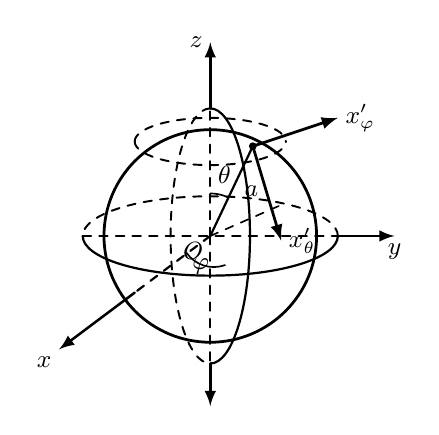
\begin{tikzpicture}[x=1.2cm, y=1.2cm, >=latex, line cap=round, line join=round]
    \draw[line width=1.0pt] (0, 0) circle (1.35cm);

    \draw[line width=0.8pt, dashed] (0, 0) -- (0, 1.35);
    \draw[line width=0.8pt, dashed] (0, 0) -- (0, -1.35);
    \draw[line width=0.9pt, ->] (0, 1.35) -- (0, 2.05) node[left=-1pt] {\small $z$};
    \draw[line width=0.9pt, ->] (0, -1.35) -- (0, -1.8);

    \draw[line width=0.8pt, dashed] (-1.35, 0) -- (1.35, 0);
    \draw[line width=0.9pt, ->] (1.35, 0) -- (1.95, 0) node[below=-1pt] {\small $y$};

    \draw[line width=0.8pt, dashed] (0, 0) -- (-0.8, -0.6);
    \draw[line width=0.9pt, ->] (-0.8, -0.6) -- (-1.6, -1.2) node[below left=-1pt] {\small $x$};
    \node[below left=-1pt] at (0, 0) {\small $O$};

    \draw[line width=0.7pt, dashed] (1.35, 0) arc[start angle=0, end angle=180, x radius=1.35, y radius=0.42];
    \draw[line width=0.8pt] (-1.35, 0) arc[start angle=180, end angle=360, x radius=1.35, y radius=0.42];

    \draw[line width=0.8pt] (0, 1.35) arc[start angle=90, end angle=-90, x radius=0.42, y radius=1.35];
    \draw[line width=0.7pt, dashed] (0, 1.35) arc[start angle=90, end angle=270, x radius=0.42, y radius=1.35];

    \draw[line width=0.7pt, dashed] (-0.8, 1.0) arc[start angle=180, end angle=360, x radius=0.8, y radius=0.25];
    \draw[line width=0.7pt, dashed] (-0.8, 1.0) arc[start angle=180, end angle=0, x radius=0.8, y radius=0.25];

    \coordinate (P) at (0.45, 0.95);
    \fill (P) circle (1.4pt);

    \draw[line width=0.8pt] (0, 0) -- (P) node[midway, right=1pt] {\small $a$};
    \draw[line width=0.6pt] (0, 0.45) arc[start angle=90, end angle=65, radius=0.45];
    \node at (0.15, 0.65) {\small $\theta$};

    \draw[line width=0.6pt, dashed] (0, 0) -- (0.8, 0.35);
    \draw[line width=0.6pt] (-0.25, -0.18) arc[start angle=215, end angle=290, radius=0.35];
    \node at (-0.1, -0.32) {\small $\varphi$};

    \draw[line width=1.0pt, ->] (P) -- ++(0.3, -1.0) node[right=-1pt] {\small $\boldsymbol{x}'_\theta$};
    \draw[line width=1.0pt, ->] (P) -- ++(0.9, 0.3) node[right=-1pt] {\small $\boldsymbol{x}'_\varphi$};
  \end{tikzpicture}
  \caption{}\label{fig:9.1.6}
\end{figure}

细心的读者会注意到 $\boldsymbol{x}'_{\theta} \times \boldsymbol{x}'_{\varphi} = F = 0$ 表明两个坐标切向量 $\boldsymbol{x}'_{\theta}$ 与 $\boldsymbol{x}'_{\varphi}$ 正交, 即 $\theta$ 线与 $\varphi$ 线为正交曲线网(\cref{fig:9.1.6}). \qedhere
\end{solution}

更一般地, 我们来求 $n - 1$ 维球面的单位法向量场.

\begin{example}\label{ex:9.1.11}
已知球心在坐标原点, 半径为 $a$ 的 $n - 1$ 维球面
\[
  S^{n-1}(a) = \left\{(x_{1}, x_{2}, \cdots, x_{n}) \in \mathbb{R}^{n} \mathrel{\Big|} \sum_{i=1}^{n}x_{i}^{2} = a^{2}\right\}, \quad a > 0.
\]
求 $n - 1$ 维球面 $S^{n-1}(a)$ 的单位法向量场、球面坐标及第一基本量.
\end{example}

\begin{solution}[解法 1]
令 $F(x_{1}, x_{2}, \cdots, x_{n}) = \sum_{i=1}^{n} x_{i}^{2} - a^{2}$, 则
\[
  F^{\prime}_{x_{i}} = 2x_{i}.
\]
因此, 单位法向量场为
\begin{align*}
  \boldsymbol{n}_{0} &= \pm\frac{1}{\sqrt{\sum_{i=1}^{n}(F_{x_{i}}^{\prime})^{2}}}(F_{x_{1}}^{\prime}, F_{x_{2}}^{\prime}, \cdots, F_{x_{n}}^{\prime}) = \pm\frac{1}{\sqrt{\sum_{i=1}^{n}(2x_{i})^{2}}}(2x_{1}, 2x_{2}, \cdots, 2x_{n}) \\
  &= \pm\left(\frac{x_{1}}{a}, \frac{x_{2}}{a}, \cdots, \frac{x_{n}}{a}\right).
\end{align*}
\end{solution}

\begin{solution}[解法 2]
设 $\boldsymbol{x}(\theta_{1}, \theta_{2}, \cdots, \theta_{n-1}) = (x_{1}(\theta_{1}, \cdots, \theta_{n-1}), x_{2}(\theta_{1}, \cdots, \theta_{n-1}), \cdots, x_{n}(\theta_{1}, \cdots, \theta_{n-1}))$, 其中
\[
  \left\{\begin{aligned}
    x_{1} &= a\cos\theta_{1}, \\
    x_{2} &= a\sin\theta_{1}\cos\theta_{2}, \\
    x_{3} &= a\sin\theta_{1}\sin\theta_{2}\cos\theta_{3}, \\
    &\;\;\vdots \\
    x_{n-1} &= a\sin\theta_{1}\sin\theta_{2}\sin\theta_{3}\cdots\sin\theta_{n-2}\cos\theta_{n-1}, \\
    x_{n} &= a\sin\theta_{1}\sin\theta_{2}\sin\theta_{3}\cdots\sin\theta_{n-2}\sin\theta_{n-1},
  \end{aligned}\right.
\]
而 $\theta_{1}, \theta_{2}, \cdots, \theta_{n-1}$ 称为球面参数, 也称为球面坐标. 不难验证第一基本量为
\[
  g_{ij} = \boldsymbol{x}^{\prime}_{\theta_{i}} \cdot \boldsymbol{x}^{\prime}_{\theta_{j}} = \left\{\begin{aligned}
    &0, && i \neq j, \\
    &a^{2}, && i = j = 1, \\
    &a^{2}\sin^{2}\theta_{1}\cdots\sin^{2}\theta_{i-1}, && i = j = 2, 3, \cdots, n - 1.
  \end{aligned}\right.
\]
由此得到 $\sqrt{\det(g_{ij})} = a^{n-1}\sin^{n-2}\theta_1\sin^{n-3}\theta_2\cdots\sin\theta_{n-2}$.

对 $\boldsymbol{x} \cdot \boldsymbol{x} = a^{2}$ 两边关于 $\theta_{i}$ 求偏导或直接对 $\boldsymbol{x}$ 关于 $\theta_{i}$ 求偏导验证得 $\boldsymbol{x} \cdot \dfrac{\partial\boldsymbol{x}}{\partial\theta_{i}} = 0$, $i = 1, 2, \cdots, n - 1$ 可知, $\boldsymbol{x}$ 为球面 $M$ 的法向量场. 因此, 单位法向量场为
\[
  \boldsymbol{n}_{0} = \pm\frac{\boldsymbol{x}}{\|\boldsymbol{x}\|} = \pm\frac{\boldsymbol{x}}{a} = \pm\left(\frac{x_{1}}{a}, \frac{x_{2}}{a}, \cdots, \frac{x_{n}}{a}\right). \qedhere
\]
\end{solution}

\begin{example}\label{ex:9.1.12}
{\emergencystretch=3em 从球面坐标, 平面极坐标 $(x_{1}, x_{2}) = (r \cos \theta, r \sin \theta)$ 以及三维 Euclid 空间 $\mathbb{R}^{3}$ 中的球坐标 $(x_{1}, x_{2}, x_{3}) = (r \cos \theta_{1}, r \sin \theta_{1} \cos \theta_{2}, r \sin \theta_{1} \sin \theta_{2})$ 或者 $(r \sin \theta \cos \varphi, r \sin \theta \sin \varphi, r \cos \theta)$(\cref{fig:9.1.7}), 自然会想到 $n$ 维 Euclid 空间 $\mathbb{R}^{n}$ 中应有球坐标.\par}

\begin{figure}[htbp]
  \centering
  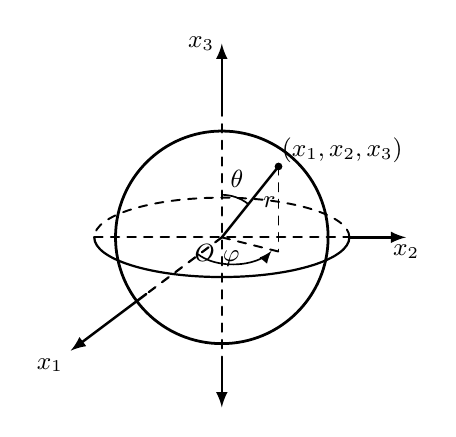
\begin{tikzpicture}[x=1.2cm, y=1.2cm, >=latex, line cap=round, line join=round]
    \draw[line width=1.0pt] (0, 0) circle (1.35cm);

    \draw[line width=0.8pt, dashed] (0, -1.35) -- (0, 1.35);
    \draw[line width=0.9pt, ->] (0, 1.35) -- (0, 2.05) node[left=-1pt] {\small $x_3$};
    \draw[line width=0.9pt, ->] (0, -1.35) -- (0, -1.8);

    \draw[line width=0.8pt, dashed] (-1.35, 0) -- (1.35, 0);
    \draw[line width=0.9pt, ->] (1.35, 0) -- (1.95, 0) node[below=-1pt] {\small $x_2$};

    \draw[line width=0.8pt, dashed] (0, 0) -- (-0.8, -0.6);
    \draw[line width=0.9pt, ->] (-0.8, -0.6) -- (-1.6, -1.2) node[below left=-1pt] {\small $x_1$};
    \node[below left=-1pt] at (0, 0) {\small $O$};

    \draw[line width=0.7pt, dashed] (1.35, 0) arc[start angle=0, end angle=180, x radius=1.35, y radius=0.42];
    \draw[line width=0.8pt] (-1.35, 0) arc[start angle=180, end angle=360, x radius=1.35, y radius=0.42];

    \coordinate (P) at (0.6, 0.75);
    \fill (P) circle (1.4pt) node[anchor=south west, inner sep=1pt] {\small $(x_1, x_2, x_3)$};

    \coordinate (Pxy) at (0.6, -0.15);
    \draw[line width=0.7pt, dashed] (P) -- (Pxy);
    \draw[line width=0.7pt, dashed] (0, 0) -- (Pxy);

    \draw[line width=0.9pt] (0, 0) -- (P) node[midway, right=1pt] {\small $r$};

    \draw[line width=0.6pt] (0, 0.45) arc[start angle=90, end angle=52, radius=0.45];
    \node at (0.16, 0.62) {\small $\theta$};

    \draw[line width=0.6pt, ->] (-0.25, -0.18) arc[start angle=215, end angle=335, x radius=0.45, y radius=0.25];
    \node at (0.1, -0.22) {\small $\varphi$};
  \end{tikzpicture}
  \caption{}\label{fig:9.1.7}
\end{figure}

$\boldsymbol{x}(r, \theta_{1}, \theta_{2}, \cdots, \theta_{n-1}) = (x_{1}(r, \theta_{1}, \cdots, \theta_{n-1}), x_{2}(r, \theta_{1}, \cdots, \theta_{n-1}), \cdots, x_{n}(r, \theta_{1}, \cdots, \theta_{n-1}))$ 为
\[
  \left\{\begin{aligned}
    x_{1} &= r\cos\theta_{1}, \\
    x_{2} &= r\sin\theta_{1}\cos\theta_{2}, \\
    x_{3} &= r\sin\theta_{1}\sin\theta_{2}\cos\theta_{3}, \\
    &\;\;\vdots \\
    x_{n-1} &= r\sin\theta_{1}\sin\theta_{2}\sin\theta_{3}\cdots\sin\theta_{n-2}\cos\theta_{n-1}, \\
    x_{n} &= r\sin\theta_{1}\sin\theta_{2}\sin\theta_{3}\cdots\sin\theta_{n-2}\sin\theta_{n-1},
  \end{aligned}\right.
\]
其中 $r, \theta_{1}, \theta_{2}, \cdots, \theta_{n-1}$ 为 $\mathbb{R}^{n}$ 的参数, 也称为球坐标. 不难验证第一基本量为
\[
  g_{00} = \boldsymbol{x}_{r}^{\prime} \cdot \boldsymbol{x}_{r}^{\prime} = 1,
\]
\[
  g_{0i} = \boldsymbol{x}_{r}^{\prime} \cdot \boldsymbol{x}_{\theta_{i}}^{\prime} = 0 = \boldsymbol{x}_{\theta_{i}}^{\prime} \cdot \boldsymbol{x}_{r}^{\prime} = g_{i0},
\]
\[
  g_{ij} = \left\{\begin{aligned}
    &0, && i \neq j, \\
    &r^{2}, && i = j = 1, \\
    &r^{2}\sin^{2}\theta_{1}\sin^{2}\theta_{2}\cdots\sin^{2}\theta_{i-1}, && i = j = 2, 3, \cdots, n - 1.
  \end{aligned}\right.
\]
由此得到
\begin{align*}
  \left(\frac{\partial(x_{1}, x_{2}, \cdots, x_{n})}{\partial(r, \theta_{1}, \theta_{2}, \cdots, \theta_{n-1})}\right)^{2}
  &= \det\begin{pmatrix}
    \dfrac{\partial x_{1}}{\partial r} & \cdots & \dfrac{\partial x_{n}}{\partial r} \\
    \dfrac{\partial x_{1}}{\partial\theta_{1}} & \cdots & \dfrac{\partial x_{n}}{\partial\theta_{1}} \\
    \vdots & & \vdots \\
    \dfrac{\partial x_{1}}{\partial\theta_{n-1}} & \cdots & \dfrac{\partial x_{n}}{\partial\theta_{n-1}}
  \end{pmatrix}\begin{pmatrix}
    \dfrac{\partial x_{1}}{\partial r} & \dfrac{\partial x_{1}}{\partial\theta_{1}} & \cdots & \dfrac{\partial x_{1}}{\partial\theta_{n-1}} \\
    \vdots & \vdots & & \vdots \\
    \dfrac{\partial x_{n}}{\partial r} & \dfrac{\partial x_{n}}{\partial\theta_{1}} & \cdots & \dfrac{\partial x_{n}}{\partial\theta_{n-1}}
  \end{pmatrix} \\
  &= \det\begin{pmatrix}
    g_{00} & g_{01} & \cdots & g_{0,n-1} \\
    g_{10} & g_{11} & \cdots & g_{1,n-1} \\
    \vdots & \vdots & & \vdots \\
    g_{n-1,0} & g_{n-1,1} & \cdots & g_{n-1,n-1}
  \end{pmatrix} \\
  &= \left[r^{n-1}\sin^{n-2}\theta_{1}\sin^{n-3}\theta_{2}\cdots\sin\theta_{n-2}\right]^{2}.
\end{align*}
如果注意到
\begin{align*}
  \frac{\partial(x_{1}, x_{2}, \cdots, x_{n})}{\partial(r, \theta_{1}, \theta_{2}, \cdots, \theta_{n-1})}\bigg|_{\left(r, \frac{\pi}{2}, \frac{\pi}{2}, \cdots, \frac{\pi}{2}\right)}
  &= \begin{vmatrix}
    0 & -r & 0 & \cdots & 0 \\
    0 & 0 & -r & \cdots & 0 \\
    \vdots & \vdots & \vdots & & \vdots \\
    0 & 0 & 0 & \cdots & -r \\
    1 & 0 & 0 & \cdots & 0
  \end{vmatrix} = (-1)^{1+n}(-r)^{n-1} \\
  &= r^{n-1} > 0,
\end{align*}
及直角坐标 $x_{1}, x_{2}, \cdots, x_{n}$ 与球坐标 $r, \theta_{1}, \theta_{2}, \cdots, \theta_{n-1}$ 之间变换的 Jacobi 行列式
\[
  \frac{\partial(x_{1}, x_{2}, \cdots, x_{n})}{\partial(r, \theta_{1}, \theta_{2}, \cdots, \theta_{n-1})}
\]
为连续函数, 它具有保号性, 因此有
\[
  \frac{\partial(x_{1}, x_{2}, \cdots, x_{n})}{\partial(r, \theta_{1}, \theta_{2}, \cdots, \theta_{n-1})} > 0.
\]
从而
\begin{align*}
  \frac{\partial(x_{1}, x_{2}, \cdots, x_{n})}{\partial(r, \theta_{1}, \theta_{2}, \cdots, \theta_{n-1})}
  &= \sqrt{\det\begin{pmatrix}
    g_{00} & g_{01} & \cdots & g_{0,n-1} \\
    g_{10} & g_{11} & \cdots & g_{1,n-1} \\
    \vdots & \vdots & & \vdots \\
    g_{n-1,0} & g_{n-1,1} & \cdots & g_{n-1,n-1}
  \end{pmatrix}} \\
  &= r^{n-1}\sin^{n-2}\theta_{1}\sin^{n-3}\theta_{2}\cdots\sin\theta_{n-2}.
\end{align*}
此行列式在应用 $n$ 元球坐标变换计算 $n$ 重积分时非常重要与简便.
\end{example}


\begin{example}\label{ex:9.1.13}
设 $U\subsetneq\mathbb{R}^{3}$ 为开集, $F, G\colon U \to \mathbb{R}^{1}$ 为两个三元函数,
\[
  L = \{(x, y, z) \in \mathbb{R}^{3} \mid F(x, y, z) = 0, \; G(x, y, z) = 0\},\quad
  \boldsymbol{x}^{0} = (x_{0}, y_{0}, z_{0}) \in L.
\]
如果 $F, G \in C^{k}(U, \mathbb{R}^{1})$, $k \geqslant 1$, 且 $\boldsymbol{x}^{0}$ 处的切向量
\[
  \boldsymbol{t}(\boldsymbol{x}^{0}) = \boldsymbol{J}\boldsymbol{F}(\boldsymbol{x}^{0}) \times
  \boldsymbol{J}\boldsymbol{G}(\boldsymbol{x}^{0}) =
  \begin{vmatrix}
    \boldsymbol{i} & \boldsymbol{j} & \boldsymbol{k} \\\\
    F_{x}^{\prime} & F_{y}^{\prime} & F_{z}^{\prime} \\\\
    G_{x}^{\prime} & G_{y}^{\prime} & G_{z}^{\prime}
  \end{vmatrix} \neq \boldsymbol{0},
\]
则 $\exists\,\boldsymbol{x}^{0}$ 的开邻域 $U_{0} \subset U$, s.\,t. $U_{0} \cap L$ 为一段 $C^{k}$ 参数曲线. 这时, $L$ 在 $\boldsymbol{x}^{0}$ 处的切线方程为
\[
  \left\{\begin{aligned}
    &F_{x}^{\prime}(\boldsymbol{x}^{0})(x - x_{0}) + F_{y}^{\prime}(\boldsymbol{x}^{0})(y - y_{0}) + F_{z}^{\prime}(\boldsymbol{x}^{0})(z - z_{0}) = 0, \\\\
    &G_{x}^{\prime}(\boldsymbol{x}^{0})(x - x_{0}) + G_{y}^{\prime}(\boldsymbol{x}^{0})(y - y_{0}) + G_{z}^{\prime}(\boldsymbol{x}^{0})(z - z_{0}) = 0.
  \end{aligned}\right.
\]

\begin{proof}
不妨设
\[
  \frac{\partial(F, G)}{\partial(y, z)}\bigg|_{\boldsymbol{x}^{0}} \neq 0.
\]
由隐函数定理, 存在含 $x_{0}$ 的开区间 $I$ 与含 $(y_{0}, z_{0})$ 的开区间 $J$ 使得方程组
\[
  F(x, y, z) = 0, \quad G(x, y, z) = 0
\]
在含 $\boldsymbol{x}^{0}$ 的开邻域 $U_{0} = I \times J$ 内有
\[
  y = f(x), \quad z = g(x), \quad x \in I,
\]
且 $f, g \in C^{k}(I, \mathbb{R}^{1})$. 因此, $U_{0} \cap L$ 为一段 $C^{k}$ 参数曲线
$\boldsymbol{x} = \boldsymbol{x}(x) = (x, f(x), g(x))$, $x$ 为其参数. 该曲线在 $\boldsymbol{x}^{0}$ 处的切向量为 $(1, f^{\prime}(x_{0}), g^{\prime}(x_{0}))$. 又因为
\[
  F(x, f(x), g(x)) \equiv 0, \quad G(x, f(x), g(x)) \equiv 0,
\]
所以
\[
  \left\{\begin{aligned}
    &F_{x}^{\prime} + F_{y}^{\prime}f^{\prime}(x) + F_{z}^{\prime}g^{\prime}(x) = 0, \\\\
    &G_{x}^{\prime} + G_{y}^{\prime}f^{\prime}(x) + G_{z}^{\prime}g^{\prime}(x) = 0,
  \end{aligned}\right.
\]
从而
\begin{align*}
  \bigl(1, f^{\prime}(x_{0}), g^{\prime}(x_{0})\bigr) \parallel \boldsymbol{t}(\boldsymbol{x}^{0})
  &= \bigl(F_{x}^{\prime}(\boldsymbol{x}^{0}), F_{y}^{\prime}(\boldsymbol{x}^{0}), F_{z}^{\prime}(\boldsymbol{x}^{0})\bigr)
     \times \bigl(G_{x}^{\prime}(\boldsymbol{x}^{0}), G_{y}^{\prime}(\boldsymbol{x}^{0}), G_{z}^{\prime}(\boldsymbol{x}^{0})\bigr) \\\\
  &= \boldsymbol{J}\boldsymbol{F}(\boldsymbol{x}^{0}) \times \boldsymbol{J}\boldsymbol{G}(\boldsymbol{x}^{0})
     \ (\text{图} \ \ref{fig:9.1.8}).
\end{align*}
\begin{figure}[htbp]
  \centering
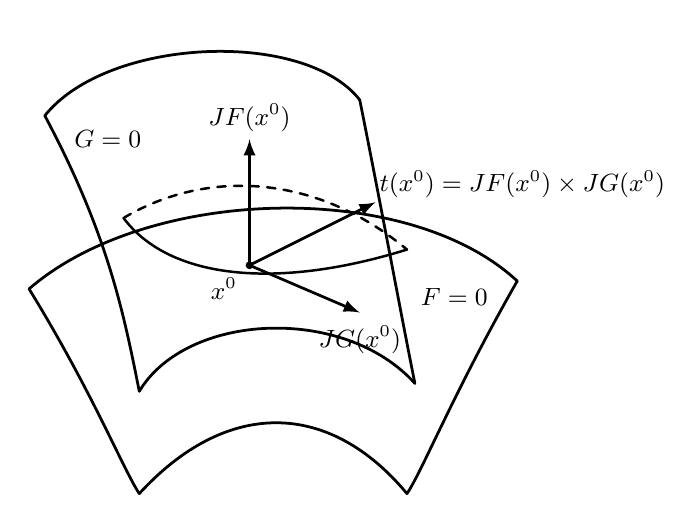
\begin{tikzpicture}[x=1.0cm, y=1.0cm, >=latex, line cap=round, line join=round]
    % 曲面 G=0 (后上)
    \draw[line width=1.0pt] (-2.8, 2.7) .. controls (-2.0, 3.7) and (0.5, 3.8) .. (1.2, 2.9);
    \draw[line width=1.0pt] (-2.8, 2.7) .. controls (-2.0, 1.2) and (-1.8, 0.2) .. (-1.6, -0.8);
    \draw[line width=1.0pt] (1.2, 2.9) .. controls (1.5, 1.4) and (1.7, 0.3) .. (1.9, -0.7);
    \draw[line width=1.0pt] (-1.6, -0.8) .. controls (-1.0, 0.2) and (1.0, 0.3) .. (1.9, -0.7);
    \node at (-2.0, 2.4) {\small $G = 0$};

    % 曲面 F=0 (横跨相交)
    \draw[line width=1.0pt] (-3.0, 0.5) .. controls (-1.5, 1.8) and (1.8, 1.9) .. (3.2, 0.6);
    \draw[line width=1.0pt] (-3.0, 0.5) .. controls (-2.2, -0.8) and (-1.8, -1.8) .. (-1.6, -2.1);
    \draw[line width=1.0pt] (3.2, 0.6) .. controls (2.4, -0.8) and (2.0, -1.8) .. (1.8, -2.1);
    \draw[line width=1.0pt] (-1.6, -2.1) .. controls (-0.5, -0.9) and (0.8, -0.9) .. (1.8, -2.1);
    \node at (2.4, 0.4) {\small $F = 0$};

    % 交线 (鞍形弧线，部分虚线)
    \draw[line width=0.9pt, dashed] (-1.8, 1.4) .. controls (-0.8, 2.0) and (0.6, 2.0) .. (1.8, 1.0);
    \draw[line width=0.9pt] (-1.8, 1.4) .. controls (-1.2, 0.6) and (0.2, 0.5) .. (1.8, 1.0);

    % 相交点 x^0
    \coordinate (X0) at (-0.2, 0.8);
    \fill (X0) circle (1.4pt) node[below left=1pt] {\small $\boldsymbol{x}^0$};

    % 法向量 JF 与 JG
    \draw[line width=1.0pt, ->] (X0) -- ++(0, 1.6) node[above=-1pt] {\small $\boldsymbol{J}F(\boldsymbol{x}^0)$};
    \draw[line width=1.0pt, ->] (X0) -- ++(1.4, -0.6) node[below=1pt] {\small $\boldsymbol{J}G(\boldsymbol{x}^0)$};

    % 切向量 t(x^0) = JF x JG
    \draw[line width=1.0pt, ->] (X0) -- ++(1.6, 0.8) node[anchor=south west, inner sep=1pt] {\small $\boldsymbol{t}(\boldsymbol{x}^0) = \boldsymbol{J}F(\boldsymbol{x}^0) \times \boldsymbol{J}G(\boldsymbol{x}^0)$};
  \end{tikzpicture}
  \caption{}\label{fig:9.1.8}
\end{figure}

由此知, 切线平行于 $\boldsymbol{t}(\boldsymbol{x}^{0})$, 而切线方程为
\[
  \left\{\begin{aligned}
    &F_{x}^{\prime}(\boldsymbol{x}^{0})(x - x_{0}) + F_{y}^{\prime}(\boldsymbol{x}^{0})(y - y_{0}) + F_{z}^{\prime}(\boldsymbol{x}^{0})(z - z_{0}) = 0, \\\\
    &G_{x}^{\prime}(\boldsymbol{x}^{0})(x - x_{0}) + G_{y}^{\prime}(\boldsymbol{x}^{0})(y - y_{0}) + G_{z}^{\prime}(\boldsymbol{x}^{0})(z - z_{0}) = 0.
  \end{aligned}\right.
\]
\qedhere
\end{proof}
\end{example}

\begin{example}\label{ex:9.1.14}
设 $\Delta \subset \mathbb{R}^{2}$ 为开区域, 曲面 $M$ 的参数表示为 $\boldsymbol{x}\colon \Delta \to \mathbb{R}^{3}$, 它是 $C^{1}$ 映射. 而 $(u(t), v(t))$ 对应于 $M$ 上的一条 $C^{1}$ 曲线, 其向量形式为
\[
  \boldsymbol{x} = \boldsymbol{x}(u(t), v(t)),
\]
\[
  \mathrm{d}\boldsymbol{x} = \bigl[\boldsymbol{x}_{u}^{\prime}u^{\prime}(t) + \boldsymbol{x}_{v}^{\prime}v^{\prime}(t)\bigr]\mathrm{d}t
  = \boldsymbol{x}_{u}^{\prime}\mathrm{d}u + \boldsymbol{x}_{v}^{\prime}\mathrm{d}v.
\]
弧元 $\mathrm{d}s$ 的平方为
\begin{align*}
  (\mathrm{d}s)^{2} &= (\mathrm{d}\boldsymbol{x})^{2} = \mathrm{d}\boldsymbol{x}\bullet\mathrm{d}\boldsymbol{x} \\\\
  &= \bigl[E{u^{\prime}}^{2}(t) + 2Fu^{\prime}(t)v^{\prime}(t) + G{v^{\prime}}^{2}(t)\bigr](\mathrm{d}t)^{2} \\\\
  &= E(\mathrm{d}u)^{2} + 2F\mathrm{d}u\mathrm{d}v + G(\mathrm{d}v)^{2}.
\end{align*}
由此得到 $M$ 上从点 $\boldsymbol{x}(u(\alpha), v(\alpha))$ 到 $\boldsymbol{x}(u(\beta), v(\beta))$ 的曲线的弧长为
\[
  s = \int_{\alpha}^{\beta}\sqrt{E\,{u^{\prime}}^{2}(t) + 2Fu^{\prime}(t)v^{\prime}(t) + G\,{v^{\prime}}^{2}(t)}\;\mathrm{d}t.
\]
考虑例 \ref{ex:9.1.10} 中的球面 $M$ 上的两点 $p$ 与 $q$. 不失一般性, 可设 $p$ 与 $q$ 在 $M$ 的同一条经线上. 设这两点的参数分别为 $(\theta_{0}, \varphi_{0})$ 与 $(\theta_{1}, \varphi_{1})$, 其中 $\theta_{1} > \theta_{0}$. 这两点所决定的球面曲线记为 $\Gamma$, 其 $C^{1}$ 参数表示为
\[
  \bigl(\theta(t), \varphi(t)\bigr), \quad t_{0} \leqslant t \leqslant t_{1}.
\]
于是, $\Gamma$ 的弧长为
\begin{align*}
  s(\Gamma) &= \int_{t_{0}}^{t_{1}}\sqrt{a^{2}\bigl[\theta^{\prime}(t)\bigr]^{2} + a^{2}\sin^{2}\theta(t) \cdot \bigl[\varphi^{\prime}(t)\bigr]^{2}}\;\mathrm{d}t \\\\
  &\geqslant a\int_{t_{0}}^{t_{1}}\theta^{\prime}(t)\mathrm{d}\theta
  = a\bigl[\theta(t_{1}) - \theta(t_{0})\bigr].
\end{align*}
式中等号成立等价于 $\varphi^{\prime}(t) = \vec{0}$ 等价于 $\varphi(t) = \varphi_{0}$ (常值). 这时曲线 $\Gamma$ 正是由 $p$ 与 $q$ 两点所决定的大圆弧, 而
$  a\bigl[\theta(t_{1}) - \theta(t_{0})\bigr] = a(\theta_{1} - \theta_{0})$ 恰为这一段大圆弧的弧长.
\end{example}

\begin{definition}\label{def:9.1.4}
设 $s$ 维 $C^{k}\,(k \geqslant 1)$ 正则曲面 $M$ 的参数表示为 $\boldsymbol{x}(u_{1}, u_{2}, \cdots, u_{s})$, 它的第一基本量为
\[
  g_{ij} = \boldsymbol{x}_{u_{i}}^{\prime} \cdot \boldsymbol{x}_{u_{j}}^{\prime}, \quad i, j = 1, 2, \cdots, s.
\]
我们称
\[
  I = \sum_{i, j = 1}^{s}g_{ij}\mathrm{d}u_{i}\mathrm{d}u_{j}
\]
为曲面 $M$ 或 $\boldsymbol{x}(\boldsymbol{u})$ 的第一基本形式. 易见,
\begin{align*}
  (\mathrm{d}\boldsymbol{x})^{2} &= \mathrm{d}\boldsymbol{x}\bullet\mathrm{d}\boldsymbol{x} \\\\
  &= \Bigl(\sum_{i=1}^{s}\boldsymbol{x}_{u_{i}}^{\prime}\mathrm{d}u_{i}\Bigr)
     \bullet \Bigl(\sum_{j=1}^{s}\boldsymbol{x}_{u_{j}}^{\prime}\mathrm{d}u_{j}\Bigr) \\\\
  &= \sum_{i, j = 1}^{s}\boldsymbol{x}_{u_{i}}^{\prime}\bullet\boldsymbol{x}_{u_{j}}^{\prime}\mathrm{d}u_{i}\mathrm{d}u_{j}
  = \sum_{i, j = 1}^{s}g_{ij}\mathrm{d}u_{i}\mathrm{d}u_{j} = I.
\end{align*}
考察 $M$ 上的曲线 $\boldsymbol{u}(t)$ 或 $\boldsymbol{x}(\boldsymbol{u}(t))$, 则弧元 $\mathrm{d}s$ 的平方为
\begin{align*}
  (\mathrm{d}s)^{2} &= (\mathrm{d}\boldsymbol{x})^{2} = \mathrm{d}\boldsymbol{x}\cdot\mathrm{d}\boldsymbol{x} \\\\
  &= \Bigl(\sum_{i=1}^{s}\boldsymbol{x}_{u_{i}}^{\prime}\mathrm{d}u_{i}\Bigr)
     \cdot \Bigl(\sum_{j=1}^{s}\boldsymbol{x}_{u_{j}}^{\prime}\mathrm{d}u_{j}\Bigr) \\\\
  &= \sum_{i, j = 1}^{s}\boldsymbol{x}_{u_{i}}^{\prime}\cdot\boldsymbol{x}_{u_{j}}^{\prime}\mathrm{d}u_{i}\mathrm{d}u_{j}
  = \sum_{i, j = 1}^{s}g_{ij}\mathrm{d}u_{i}\mathrm{d}u_{j},
\end{align*}
其中 $\mathrm{d}u_{i} = \mathrm{d}u_{i}(t) = u_{i}^{\prime}(t)\mathrm{d}t$. 从 $t_{0}$ 到 $t_{1}$ 相应的弧长为
\[
  s\bigg|_{t_{0}}^{t_{1}} = \int_{t_{0}}^{t_{1}}\sqrt{\sum_{i, j = 1}^{s}g_{ij}u_{i}^{\prime}u_{j}^{\prime}}\;\mathrm{d}t.
\]
当 $s = 2$ 时, $g_{11} = E$, $g_{12} = g_{21} = F$, $g_{22} = G$, 由 $\boldsymbol{x}_{u}^{\prime}\mathrm{d}u$ 与 $\boldsymbol{x}_{v}^{\prime}\mathrm{d}v$ 张成的平行四边形的面积
\begin{align*}
  \mathrm{d}\boldsymbol{\sigma} &= \bigl\lVert\boldsymbol{x}_{u}^{\prime}\mathrm{d}u \times \boldsymbol{x}_{v}^{\prime}\mathrm{d}v\bigr\rVert
  = \bigl\lVert\boldsymbol{x}_{u}^{\prime} \times \boldsymbol{x}_{v}^{\prime}\bigr\rVert\mathrm{d}u\mathrm{d}v \\\\
  &= \sqrt{EG - F^{2}}\;\mathrm{d}u\mathrm{d}v
\end{align*}
称为该曲面的面积元, 也称为二维体积元(图 \ref{fig:9.1.9}).

\begin{figure}[htbp]
  \centering
\begin{tikzpicture}[x=1.0cm, y=1.0cm, >=latex, line cap=round, line join=round]
    % 曲面 M
    \draw[line width=1.0pt] (-0.2, 2.0) .. controls (1.0, 2.8) and (3.0, 2.8) .. (4.0, 1.6);
    \draw[line width=1.0pt] (-0.2, 2.0) .. controls (0.6, 1.4) and (1.4, 1.5) .. (2.2, 0.8)
                            .. controls (3.0, 1.1) and (3.6, 1.2) .. (4.0, 1.6);
    \node at (3.8, 1.2) {\small $M$};

    \coordinate (XUV) at (1.5, 1.8);

    % 参数网格虚线
    \draw[line width=0.8pt, dashed] (0.3, 1.4) .. controls (1.0, 2.0) and (1.5, 2.3) .. (3.4, 2.3);
    \draw[line width=0.8pt] (0.8, 2.5) .. controls (1.3, 2.0) and (2.0, 1.5) .. (2.7, 0.8);

    % 切平面 (平行四边形外框)
    \coordinate (TP1) at (0.5, 1.8);
    \coordinate (TP2) at (1.6, 3.2);
    \coordinate (TP3) at (3.5, 2.6);
    \coordinate (TP4) at (2.4, 1.2);
    \draw[line width=0.8pt] (TP1) -- (TP2) -- (TP3) -- (TP4) -- cycle;

    % 微元面积平行四边形 (带阴影)
    \coordinate (DP1) at (XUV);
    \coordinate (DP2) at ($(XUV) + (0.3, 1.1)$);
    \coordinate (DP3) at ($(XUV) + (1.5, 1.15)$);
    \coordinate (DP4) at ($(XUV) + (1.2, 0.05)$);

    \fill[pattern=north east lines, pattern color=black!70] (DP1) -- (DP2) -- (DP3) -- (DP4) -- cycle;
    \draw[line width=0.9pt] (DP1) -- (DP2) -- (DP3) -- (DP4) -- cycle;

    % 微元边向量
    \draw[line width=1.0pt, ->] (DP1) -- (DP4) node[right=-1pt] {\small $\boldsymbol{x}'_u \mathrm{d}u$};
    \draw[line width=1.0pt, ->] (DP1) -- (DP2) node[above=-1pt] {\small $\boldsymbol{x}'_v \mathrm{d}v$};

    \fill (XUV) circle (1.4pt) node[below=2pt] {\small $\boldsymbol{x}(u,v)$};
  \end{tikzpicture}
  \caption{}\label{fig:9.1.9}
\end{figure}

更一般地, 由 $\boldsymbol{x}_{u_{i}}^{\prime}\mathrm{d}u_{i}$, $i = 1, 2, \cdots, s$ 张成的 $s$ 维平行 $2s$ 面体的体积
\[
  \mathrm{d}\sigma = \sqrt{\det(g_{ij})}\;\mathrm{d}u_{1}\mathrm{d}u_{2}\cdots\mathrm{d}u_{s}
\]
称为该 $s$ 维曲面的 $s$ 维体积元.
\end{definition}

\begin{example}\label{ex:9.1.15}
求下列曲面的第一基本形式及体积元:

(1) $\mathbb{R}^{3}$ 中二维曲面 $M$, 参数表示为 $\boldsymbol{x}(x, y) = (x, y, z(x, y))$, $z(x, y)$ 为 $C^{1}$ 函数;

(2) $\mathbb{R}^{3}$ 中二维球面 $S^{2}(a)$, 参数表示为
$\boldsymbol{x}(\theta, \varphi) = (a\sin\theta\cos\varphi, a\sin\theta\sin\varphi, a\cos\theta)$, $a > 0$;

(3) $\mathbb{R}^{n}$ 中 $n-1$ 维球面 $S^{n-1}(a)$, 参数表示 $\boldsymbol{x}(\theta_{1}, \theta_{2}, \cdots, \theta_{n-1})$, 如例 \ref{ex:9.1.11} 所示;

(4) $\mathbb{R}^{n}$ 中 $n$ 维参数曲面 $\boldsymbol{x}(r, \theta_{1}, \theta_{2}, \cdots, \theta_{n-1})$, 如例 \ref{ex:9.1.12} 所示.

\begin{solution}
(1) 因为
\[
  \boldsymbol{x}_{x}^{\prime} = (1, 0, z_{x}^{\prime}), \quad \boldsymbol{x}_{y}^{\prime} = (0, 1, z_{y}^{\prime}),
\]
\[
  \begin{pmatrix} g_{11} & g_{12} \\ g_{21} & g_{22} \end{pmatrix}
  = \begin{pmatrix} E & F \\ F & G \end{pmatrix}
  = \begin{pmatrix} 1 + {z^{\prime}}_{x}^{2} & z_{x}^{\prime}z_{y}^{\prime} \\ z_{x}^{\prime}z_{y}^{\prime} & 1 + {z^{\prime}}_{y}^{2} \end{pmatrix},
\]
所以, 曲面 $M$ 的第一基本形式为
\begin{align*}
  I &= E(\mathrm{d}x)^{2} + 2F\mathrm{d}x\mathrm{d}y + G(\mathrm{d}y)^{2} \\\\
  &= (1 + {z_{x}^{\prime}}^{2})(\mathrm{d}x)^{2} + 2z_{x}^{\prime}z_{y}^{\prime}\mathrm{d}x\mathrm{d}y
     + (1 + {z_{y}^{\prime}}^{2})(\mathrm{d}y)^{2}. \qedhere
\end{align*}
而面积元为
\begin{align*}
  \mathrm{d}\sigma &= \sqrt{EG - F^{2}}\;\mathrm{d}x\mathrm{d}y \\\\
  &= \sqrt{(1 + {z_{x}^{\prime}}^{2})(1 + {z_{y}^{\prime}}^{2}) - (z_{x}^{\prime}z_{y}^{\prime})^{2}}\;\mathrm{d}x\mathrm{d}y \\\\
  &= \sqrt{1 + {z_{x}^{\prime}}^{2} + {z_{y}^{\prime}}^{2}}\;\mathrm{d}x\mathrm{d}y.
\end{align*}

(2) 由例 \ref{ex:9.1.10} 解法 2 知, 二维球面 $M$ 的第一基本形式为
\[
  I = a^{2}(\mathrm{d}\theta)^{2} + a^{2}\sin^{2}\theta(\mathrm{d}\varphi)^{2}.
\]
而面积元为
\[
  \mathrm{d}\sigma = \sqrt{EG - F^{2}}\;\mathrm{d}\theta\mathrm{d}\varphi = a^{2}\sin\theta\;\mathrm{d}\theta\mathrm{d}\varphi.
\]

(3) 由例 \ref{ex:9.1.11} 的解法 2 知, $n-1$ 维球面 $S^{n-1}(a)$ 的第一基本形式为
\begin{align*}
  I &= a^{2}(\mathrm{d}\theta_{1})^{2} + a^{2}\sin^{2}\theta_{1}(\mathrm{d}\theta_{2})^{2} + \cdots
     + a^{2}\sin^{2}\theta_{1}\cdots\sin^{2}\theta_{i-1}(\mathrm{d}\theta_{i})^{2} \\\\
  &\quad + \cdots + a^{2}\sin^{2}\theta_{1}\cdots\sin^{2}\theta_{n-2}(\mathrm{d}\theta_{n-1})^{2}.
\end{align*}
而面积元为
\begin{align*}
  \mathrm{d}\sigma &= \sqrt{\det(g_{ij})}\;\mathrm{d}\theta_{i}\mathrm{d}\theta_{i+1}\cdots\mathrm{d}\theta_{n-1} \\\\
  &= a^{n-1}\sin^{n-2}\theta_{1}\sin^{n-3}\theta_{2}\cdots\sin^{2}\theta_{n-3}\sin\theta_{n-2}
     \;\mathrm{d}\theta_{1}\mathrm{d}\theta_{2}\cdots\mathrm{d}\theta_{n-1}.
\end{align*}

(4) 由例 \ref{ex:9.1.12} 知, $\boldsymbol{x}(r, \theta_{1}, \theta_{2}, \cdots, \theta_{n-1})$ 的第二基本形式为(原文如此)
\begin{align*}
  I &= \mathrm{d}r^{2} + r^{2}(\mathrm{d}\theta_{1})^{2} + r^{2}\sin^{2}\theta_{1}(\mathrm{d}\theta_{2})^{2} + \cdots \\\\
  &\quad + r^{2}\sin^{2}\theta_{1}\cdots\sin^{2}\theta_{i-1}(\mathrm{d}\theta_{i})^{2}
  + \cdots + r^{2}\sin^{2}\theta_{1}\cdots\sin^{2}\theta_{n-2}(\mathrm{d}\theta_{n-1})^{2}.
\end{align*}
而体积元为
\begin{align*}
  \mathrm{d}v &= \sqrt{\det(g_{ij})}\;\mathrm{d}r\mathrm{d}\theta_{1}\mathrm{d}\theta_{2}\cdots\mathrm{d}\theta_{n-1} \\\\
  &= r^{n-1}\sin^{n-2}\theta_{1}\sin^{n-3}\theta_{2}\cdots\sin^{2}\theta_{n-3}\sin\theta_{n-2}
     \;\mathrm{d}r\mathrm{d}\theta_{1}\mathrm{d}\theta_{2}\cdots\mathrm{d}\theta_{n-1}. \qedhere
\end{align*}
\end{solution}
\end{example}

\begin{exblock}{练习题 9.1}
  \item 求下列曲面在指定点处的法向量, 切平面方程与法线方程:

  (1) $x^{2} + y^{2} + z^{2} = 4$, $\boldsymbol{x}^{0} = \left(1, 1, \sqrt{2}\right)$;

  (2) $z = \arctan \dfrac{y}{x}$, $\boldsymbol{x}^{0} = \left(1, 1, \dfrac{\pi}{4}\right)$;

  (3) $3x^{2} + 2y^{2} - 2z - 1 = 0$, $\boldsymbol{x}^{0} = (1, 1, 2)$;

  (4) $z = y + \ln\left(\dfrac{x}{z}\right)$, $\boldsymbol{x}^{0} = (1, 1, 1)$;

  (5) $y - \mathrm{e}^{2x - z} = 0$, $\dot{\boldsymbol{x}}^{0} = (1, 1, 2)$;

  (6) $\dfrac{x^{2}}{a^{2}} + \dfrac{y^{2}}{b^{2}} + \dfrac{z^{2}}{c^{2}} = 1$,
  $\boldsymbol{x}^{0} = \left(\dfrac{a}{\sqrt{3}}, \dfrac{b}{\sqrt{3}}, \dfrac{c}{\sqrt{3}}\right)$.

  \item 求椭球面 $x^{2} + 2y^{2} + 3z^{2} = 21$ 上所有平行于平面 $x + 4y + 6z = 0$ 的切平面.

  \item 求曲面 $x^{2} + y^{2} + z^{2} = x$ 的切平面, 使其垂直于平面 $x - y - z = 2$ 与 $x - y - \dfrac{z}{2} = 2$.

  \item 求两曲面
  \[ F(x, y, z) = 0, \quad G(x, y, z) = 0 \]
  的交线在 $xOy$ 平面上的投影曲线的切线方程, 并给出求切线方程的条件.

  \item 两相交曲面在交点处的法向量所夹的角称为这两曲面在这一点的夹角. 求圆柱面 $x^{2} + y^{2} = a^{2}$ 与曲面 $bz = xy$ 的夹角.

  \item 求椭球面
  \[ \frac{x^{2}}{a^{2}} + \frac{y^{2}}{b^{2}} + \frac{z^{2}}{c^{2}} = 1 \]
  上的点的法向量与 $x$ 轴和 $z$ 轴夹成等角的点的全体.

  \item 定出正数 $\lambda$, 使曲面 $xyz = \lambda$ 与椭球面
  \[ \frac{x^{2}}{a^{2}} + \frac{y^{2}}{b^{2}} + \frac{z^{2}}{c^{2}} = 1 \]
  在某一点相切, 即有共同的切平面.

  \item 证明: 曲面 $z = x\mathrm{e}^{\frac{x}{y}}$ 上所有切平面都通过原点.

  \item 证明: 曲面 $\sqrt{x} + \sqrt{y} + \sqrt{z} = \sqrt{a}\,(a > 0)$ 的切平面在各坐标平面上割下的诸线段之和为常数.

  \item 证明: 曲面 $F(x - az, y - bz) = 0$ 的所有切平面与某一直线平行, 其中 $a$, $b$ 为常数. 并说明论述中需加什么条件.

  \item 证明: 曲面 $F\left(\dfrac{x-a}{z-c}, \dfrac{y-b}{z-c}\right) = 0$ 的切平面通过一个固定点, 其中 $a$, $b$, $c$ 为常数. 并说明论述中需加什么条件.

  \item 证明: 曲面 $ax + by + cz = \Phi(x^{2} + y^{2} + z^{2})$ 在点 $\boldsymbol{x}^{0} = (x_{0}, y_{0}, z_{0})$ 处的法向量与向量 $(x_{0}, y_{0}, z_{0})$ 和 $(a, b, c)$ 共面. 并说明论述中需加什么条件.

  \item 求下列曲面的 $E$, $F$ 与 $G$, 第一基本形式及面积元:

  (1) 椭球面 $\boldsymbol{x}(u, v) = (a\sin u\cos v, b\sin u\sin v, c\cos u)$;

  (2) 单叶双曲面 $\boldsymbol{x}(u, v) = (a\,\mathrm{ch}\,u\cos v, b\,\mathrm{ch}\,u\sin v, c\,\mathrm{sh}\,u)$;

  (3) 椭圆抛物面 $\boldsymbol{x}(u, v) = \left(u, v, \dfrac{1}{2}\left(\dfrac{u^{2}}{a^{2}} + \dfrac{v^{2}}{b^{2}}\right)\right)$;

  (4) 双曲抛物面 $\boldsymbol{x}(u, v) = (a(u + v), b(u - v), 2uv)$;

  (5) 劈锥面 $\boldsymbol{x}(u, v) = (u\cos v, u\sin v, \varphi(v))$;

  (6) 一般螺面 $\boldsymbol{x}(u, v) = (u\cos v, u\sin v, \varphi(u) + av)$.

  \item 求 $\mathbb{R}^{3}$ 中圆柱面 $\boldsymbol{x}(\theta, z) = (a\cos\theta, a\sin\theta, z)$ 的第一基本形式与面积元.

  \item 设曲面 $M$ 的第一基本形式为
  \[ I = \mathrm{d}u^{2} + (u^{2} + a^{2})\mathrm{d}v^{2}, \]
  求曲面上的曲线 $u = v$ 从 $v_{1}$ 到 $v_{2}\,(> v_{1})$ 这一段的弧长.

  \item 求平面曲线(星形线) $x^{\frac{2}{3}} + y^{\frac{2}{3}} = a^{\frac{2}{3}}\,(a > 0)$ 上任一点处的切线方程, 并证明这些切线被坐标轴所截取的线段等长(应用 $F(x, y) = x^{\frac{2}{3}} + y^{\frac{2}{3}} - a^{\frac{2}{3}} = 0$ 与参数表示 $(x, y) = (a\cos^{3}t, a\sin^{3}t)$ 两种方法求曲线的切向量).

  \item 求下列曲线所示点处的切线与法平面:

  (1) $(x, y, z) = (a\sin^{2}t, b\sin t\cos t, c\cos^{2}t)$, 在点 $t = \dfrac{\pi}{4}$;

  (2) $2x^{2} + 3y^{2} + z^{2} = 9$, $z^{2} = 3x^{2} + y^{2}$, 在点 $(1, -1, -2)$.

  \item 证明: 球面 $x^{2} + y^{2} + z^{2} = \rho^{2}$ 与锥面 $x^{2} + y^{2} = z^{2}\tan^{2}\varphi$ 是正交的($\rho > 0$ 与 $\varphi$ 为常数).

  \item 在曲线 $(x, y, z) = (t, t^{2}, t^{3})$ 上求出一点, 使曲线在此点的切线平行于平面 $x + 2y + z = 4$.

  \item 求函数
  \[ u = \frac{x}{\sqrt{x^{2} + y^{2} + z^{2}}} \]
  沿曲线 $(x, y, z) = (t, 2t^{2}, -2t^{4})$ 在点 $(1, 2, -2)$ 处切线方向的方向导数.

  \item {\emergencystretch=3em 设 $(x_{0}, y_{0}, z_{0})$ 为曲面 $F(x, y, z) = 1$ 的非奇异点(若
  $\bigl(F_{x}^{\prime}(x_{0}, y_{0}, z_{0}),\allowbreak F_{y}^{\prime}(x_{0}, y_{0}, z_{0}),\allowbreak F_{z}^{\prime}(x_{0}, y_{0}, z_{0})\bigr) \neq (0, 0, 0)$, 则称 $(x_{0}, y_{0}, z_{0})$ 为非奇异点; 否则 $(x_{0}, y_{0}, z_{0})$ 称为奇异点), $F$ 在 $(x_{0}, y_{0}, z_{0})$ 的开邻域 $U$ 内可微, 且为 $n$ 次齐次函数. 证明: 曲面在 $(x_{0}, y_{0}, z_{0})$ 处的切平面方程为\par}
  \[
    xF_{x}^{\prime}(x_{0}, y_{0}, z_{0}) + yF_{y}^{\prime}(x_{0}, y_{0}, z_{0})
    + zF_{z}^{\prime}(x_{0}, y_{0}, z_{0}) = n.
  \]

  \item 设 $F(u, v)$ 为 $C^{1}$ 函数, 证明: 曲面 $F(nx - lz, ny - mz) = 0$ 上任一点的切平面都平行于直线 $L\colon \dfrac{x}{l} = \dfrac{y}{m} = \dfrac{z}{n}$.

  \item 从原点向单叶双曲面
  \[ \frac{x^{2}}{a^{2}} + \frac{y^{2}}{b^{2}} - \frac{z^{2}}{c^{2}} = 1 \]
  的切平面引垂线, 求垂足的轨迹.

  \item 设 $a > 0$, $b > 0$, $c > 0$. 证明: $\mathbb{R}^{3}$ 中任意一点 $(x, y, z)$ 处, 有三个彼此正交的二次曲面
  \[ \frac{x^{2}}{a^{2} - \lambda_{i}^{2}} + \frac{y^{2}}{b^{2} - \lambda_{i}^{2}} + \frac{z^{2}}{c^{2} - \lambda_{i}^{2}} = -1, \quad i = 1, 2, 3, \]
  其中 $\lambda_{1}, \lambda_{2}, \lambda_{3}$ 为三个彼此不同的实数.
\end{exblock}


\section{$n$ 元函数的极值与最值}\label{sec:9.2}

在第一册中, 我们学习过一元函数的极值与最值, 在这一节中将把这些概念与方法推广到 $n$ 元函数中去.

\begin{definition}\label{def:9.2.1}
设 $D \subset \mathbb{R}^{n}$ 为开集, $f\colon D \to \mathbb{R}^{1}$ 为 $n$ 元函数, $\boldsymbol{x}^{0} \in D$. 若存在 $\boldsymbol{x}^{0}$ 的开邻域 $U \subset D$, 使得对于 $\forall \boldsymbol{x} \in U \setminus \{\boldsymbol{x}^{0}\}$, 都有
\[
  f(\boldsymbol{x}) \leqslant f(\boldsymbol{x}^{0}) \quad (\text{或 } f(\boldsymbol{x}) \geqslant f(\boldsymbol{x}^{0})),
\]
则称 $f$ 在 $\boldsymbol{x}^{0}$ 取\textbf{极大值}(或\textbf{极小值}), 相应的点 $\boldsymbol{x}^{0}$ 称为 $f$ 的\textbf{极大值点}(或\textbf{极小值点}). 极大值与极小值统称为\textbf{极值}, 极大值点与极小值点统称为\textbf{极值点}.

如果对于 $\forall \boldsymbol{x} \in U \setminus \{\boldsymbol{x}^{0}\}$, 都有严格不等式
\[
  f(\boldsymbol{x}) < f(\boldsymbol{x}^{0}) \quad (\text{或 } f(\boldsymbol{x}) > f(\boldsymbol{x}^{0})),
\]
则称 $f$ 在 $\boldsymbol{x}^{0}$ 取\textbf{严格极大值}(或\textbf{严格极小值}), 点 $\boldsymbol{x}^{0}$ 称为 $f$ 的\textbf{严格极大值点}(或\textbf{严格极小值点}).
\end{definition}

从一元函数的知识知道, 若 $f(x)$ 在 $x_{0}$ 处取得极值, 且 $f'(x_{0})$ 存在, 则必有 $f'(x_{0}) = 0$. 这个结论对多元函数也是成立的.

\begin{theorem}[极值的必要条件]\label{thm:9.2.1}
设 $D \subset \mathbb{R}^{n}$ 为开集, $f\colon D \to \mathbb{R}^{1}$ 为 $n$ 元函数, $\boldsymbol{x}^{0} \in D$ 为 $f$ 的极值点. 若偏导数 $\dfrac{\partial f}{\partial x_{i}}(\boldsymbol{x}^{0})$ ($i = 1, 2, \cdots, n$) 存在, 则必有
\[
  \frac{\partial f}{\partial x_{i}}(\boldsymbol{x}^{0}) = 0 \quad (i = 1, 2, \cdots, n).
\]
即 $\operatorname{grad}f(\boldsymbol{x}^{0}) = \boldsymbol{0}$.
\end{theorem}

\begin{proof}
不妨设 $\boldsymbol{x}^{0}$ 为 $f$ 的极大值点. 于是存在 $\boldsymbol{x}^{0}$ 的球形开邻域 $B(\boldsymbol{x}^{0}, \delta) \subset D$, 使得对于 $\forall \boldsymbol{x} \in B(\boldsymbol{x}^{0}, \delta)$, 都有
\[
  f(\boldsymbol{x}) \leqslant f(\boldsymbol{x}^{0}).
\]
固定其余变量 $x_{j} = x_{j}^{0}$ ($j \neq i$), 令 $x_{i} \in (x_{i}^{0} - \delta, x_{i}^{0} + \delta)$, 考查一元函数
\[
  g_{i}(x_{i}) = f(x_{1}^{0}, \cdots, x_{i-1}^{0}, x_{i}, x_{i+1}^{0}, \cdots, x_{n}^{0}).
\]
显然, $g_{i}(x_{i})$ 在区间 $(x_{i}^{0} - \delta, x_{i}^{0} + \delta)$ 内于点 $x_{i}^{0}$ 处取得极大值. 又因为偏导数 $\dfrac{\partial f}{\partial x_{i}}(\boldsymbol{x}^{0})$ 存在, 所以一元函数导数 $g_{i}'(x_{i}^{0})$ 存在, 且 $g_{i}'(x_{i}^{0}) = \dfrac{\partial f}{\partial x_{i}}(\boldsymbol{x}^{0})$. 根据一元函数极值的必要条件(Fermat 定理), 必有
\[
  g_{i}'(x_{i}^{0}) = \frac{\partial f}{\partial x_{i}}(\boldsymbol{x}^{0}) = 0 \quad (i = 1, 2, \cdots, n).
\]
这就证明了 $\operatorname{grad}f(\boldsymbol{x}^{0}) = \boldsymbol{0}$.
\end{proof}

满足 $\operatorname{grad}f(\boldsymbol{x}^{0}) = \boldsymbol{0}$ 的点 $\boldsymbol{x}^{0}$ 称为函数 $f$ 的\textbf{驻点}(或\textbf{稳定点}). 定理 \ref{thm:9.2.1} 表明: 可微函数的极值点必为驻点. 但反过来, 驻点不一定是极值点, 例如函数 $f(x, y) = xy$, 在原点 $(0, 0)$ 处显然有 $f_{x}'(0, 0) = 0$, $f_{y}'(0, 0) = 0$, 所以 $(0, 0)$ 为驻点. 但是在原点的任何开邻域内, 都有点使得 $f(x, y) > 0$ (第一、三象限), 也有点使得 $f(x, y) < 0$ (第二、四象限), 而 $f(0, 0) = 0$, 故 $(0, 0)$ 不是极值点(此点称为鞍点).

因此, 驻点只是极值的必要条件, 还必须寻求极值的充分条件.

回忆一元函数 $f(x)$ 极值的充分条件: 若 $f'(x_{0}) = 0$, 且 $f''(x_{0})$ 存在, 则当 $f''(x_{0}) > 0$ 时, $x_{0}$ 为严格极小值点; 当 $f''(x_{0}) < 0$ 时, $x_{0}$ 为严格极大值点. 对于多元函数, 二阶导数由 Hesse 矩阵代替.

设 $f\colon D \to \mathbb{R}^{1}$ 具有二阶连续偏导数, 即 $f \in C^{2}(D, \mathbb{R}^{1})$, 则 $f$ 在点 $\boldsymbol{x}^{0}$ 处的 Hesse 矩阵为
\[
  \boldsymbol{H}f(\boldsymbol{x}^{0}) = \left(\frac{\partial^{2}f}{\partial x_{i}\partial x_{j}}(\boldsymbol{x}^{0})\right)_{n \times n}.
\]
由 Schwarz 定理知, $\boldsymbol{H}f(\boldsymbol{x}^{0})$ 为实对称矩阵. 二次型
\[
  Q(\boldsymbol{h}) = \boldsymbol{h} \boldsymbol{H}f(\boldsymbol{x}^{0}) \boldsymbol{h}^{\mathrm{T}} = \sum_{i,j=1}^{n} \frac{\partial^{2}f}{\partial x_{i}\partial x_{j}}(\boldsymbol{x}^{0}) h_{i} h_{j}
\]
称为 $f$ 在 $\boldsymbol{x}^{0}$ 处的 Hesse 二次型.

\begin{theorem}[极值的充分条件]\label{thm:9.2.2}
设 $D \subset \mathbb{R}^{n}$ 为开集, $f \in C^{2}(D, \mathbb{R}^{1})$, $\boldsymbol{x}^{0} \in D$ 为 $f$ 的驻点, 即 $\operatorname{grad}f(\boldsymbol{x}^{0}) = \boldsymbol{0}$.
\begin{enumerate}
  \item 若 Hesse 矩阵 $\boldsymbol{H}f(\boldsymbol{x}^{0})$ 为\textbf{正定矩阵}, 则 $\boldsymbol{x}^{0}$ 为 $f$ 的严格极小值点;
  \item 若 Hesse 矩阵 $\boldsymbol{H}f(\boldsymbol{x}^{0})$ 为\textbf{负定矩阵}, 则 $\boldsymbol{x}^{0}$ 为 $f$ 的严格极大值点;
  \item 若 Hesse 矩阵 $\boldsymbol{H}f(\boldsymbol{x}^{0})$ 为\textbf{不定矩阵}, 则 $\boldsymbol{x}^{0}$ 不是 $f$ 的极值点(称为鞍点);
  \item 若 Hesse 矩阵 $\boldsymbol{H}f(\boldsymbol{x}^{0})$ 为\textbf{半正定或半负定矩阵}, 则不能断定 $\boldsymbol{x}^{0}$ 是否为极值点, 需另作分析.
\end{enumerate}
\end{theorem}

\begin{proof}
因为 $\boldsymbol{x}^{0} \in D$, $D$ 为开集, 故存在 $\delta_{0} > 0$, 使得球形开邻域 $B(\boldsymbol{x}^{0}, \delta_{0}) \subset D$. 对于任意满足 $0 < \|\boldsymbol{h}\| < \delta_{0}$ 的向量 $\boldsymbol{h} = (h_{1}, h_{2}, \cdots, h_{n})$, 线段 $\{\boldsymbol{x}^{0} + t\boldsymbol{h} \mid 0 \leqslant t \leqslant 1\} \subset B(\boldsymbol{x}^{0}, \delta_{0})$.

根据多元函数的 Taylor 公式(带 Lagrange 余项, 见\cref{thm:8.3.1}), 存在 $\theta \in (0, 1)$, 使得
\[
  f(\boldsymbol{x}^{0} + \boldsymbol{h}) = f(\boldsymbol{x}^{0}) + \sum_{i=1}^{n}\frac{\partial f}{\partial x_{i}}(\boldsymbol{x}^{0}) h_{i} + \frac{1}{2}\sum_{i,j=1}^{n}\frac{\partial^{2}f}{\partial x_{i}\partial x_{j}}(\boldsymbol{x}^{0} + \theta\boldsymbol{h}) h_{i} h_{j}.
\]
因为 $\boldsymbol{x}^{0}$ 是驻点, 所以 $\sum_{i=1}^{n}\dfrac{\partial f}{\partial x_{i}}(\boldsymbol{x}^{0}) h_{i} = 0$. 于是
\[
  f(\boldsymbol{x}^{0} + \boldsymbol{h}) - f(\boldsymbol{x}^{0}) = \frac{1}{2}\sum_{i,j=1}^{n}\frac{\partial^{2}f}{\partial x_{i}\partial x_{j}}(\boldsymbol{x}^{0} + \theta\boldsymbol{h}) h_{i} h_{j}.
\]
记 $a_{ij} = \dfrac{\partial^{2}f}{\partial x_{i}\partial x_{j}}(\boldsymbol{x}^{0})$, $\alpha_{ij}(\boldsymbol{h}) = \dfrac{\partial^{2}f}{\partial x_{i}\partial x_{j}}(\boldsymbol{x}^{0} + \theta\boldsymbol{h}) - \dfrac{\partial^{2}f}{\partial x_{i}\partial x_{j}}(\boldsymbol{x}^{0})$. 由于 $f \in C^{2}(D, \mathbb{R}^{1})$, 当 $\|\boldsymbol{h}\| \to 0$ 时, $\alpha_{ij}(\boldsymbol{h}) \to 0$ ($i, j = 1, 2, \cdots, n$).

令 $\boldsymbol{u} = \dfrac{\boldsymbol{h}}{\|\boldsymbol{h}\|}$, 则 $\boldsymbol{u}$ 是单位向量, 即 $\|\boldsymbol{u}\| = 1$, 且 $h_{i} = \|\boldsymbol{h}\| u_{i}$. 代入上式得
\[
  f(\boldsymbol{x}^{0} + \boldsymbol{h}) - f(\boldsymbol{x}^{0}) = \frac{1}{2} \|\boldsymbol{h}\|^{2} \left[ \sum_{i,j=1}^{n} a_{ij} u_{i} u_{j} + \sum_{i,j=1}^{n} \alpha_{ij}(\boldsymbol{h}) u_{i} u_{j} \right].
\]
注意到单位球面 $S^{n-1} = \{\boldsymbol{u} \in \mathbb{R}^{n} \mid \|\boldsymbol{u}\| = 1\}$ 是 $\mathbb{R}^{n}$ 中的紧致集. 二次函数 $Q(\boldsymbol{u}) = \sum_{i,j=1}^{n} a_{ij} u_{i} u_{j}$ 在 $S^{n-1}$ 上连续.

(1) 若 $\boldsymbol{H}f(\boldsymbol{x}^{0})$ 正定, 则对于任意 $\boldsymbol{u} \in S^{n-1}$, 都有 $Q(\boldsymbol{u}) > 0$. 由连续函数在紧致集上能达到最小值, 设
\[
  m = \min_{\boldsymbol{u} \in S^{n-1}} Q(\boldsymbol{u}) > 0.
\]
另一方面, 设 $\alpha(\boldsymbol{h}) = \max_{1 \leqslant i,j \leqslant n} |\alpha_{ij}(\boldsymbol{h})|$. 因为 $|u_{i}| \leqslant 1$, 所以
\[
  \left| \sum_{i,j=1}^{n} \alpha_{ij}(\boldsymbol{h}) u_{i} u_{j} \right| \leqslant \sum_{i,j=1}^{n} |\alpha_{ij}(\boldsymbol{h})| \leqslant n^{2} \alpha(\boldsymbol{h}).
\]
由于当 $\|\boldsymbol{h}\| \to 0$ 时 $\alpha(\boldsymbol{h}) \to 0$, 故存在 $\delta \in (0, \delta_{0})$, 当 $0 < \|\boldsymbol{h}\| < \delta$ 时, $n^{2} \alpha(\boldsymbol{h}) < \dfrac{m}{2}$. 从而
\[
  \sum_{i,j=1}^{n} a_{ij} u_{i} u_{j} + \sum_{i,j=1}^{n} \alpha_{ij}(\boldsymbol{h}) u_{i} u_{j} \geqslant m - \frac{m}{2} = \frac{m}{2} > 0.
\]
因此, 当 $0 < \|\boldsymbol{h}\| < \delta$ 时,
\[
  f(\boldsymbol{x}^{0} + \boldsymbol{h}) - f(\boldsymbol{x}^{0}) \geqslant \frac{1}{4} m \|\boldsymbol{h}\|^{2} > 0.
\]
即 $f(\boldsymbol{x}^{0} + \boldsymbol{h}) > f(\boldsymbol{x}^{0})$, 这证明了 $\boldsymbol{x}^{0}$ 为 $f$ 的严格极小值点.

(2) 若 $\boldsymbol{H}f(\boldsymbol{x}^{0})$ 负定, 则考虑 $-f$, 其 Hesse 矩阵 $\boldsymbol{H}(-f)(\boldsymbol{x}^{0}) = -\boldsymbol{H}f(\boldsymbol{x}^{0})$ 为正定矩阵. 由 (1) 知 $\boldsymbol{x}^{0}$ 为 $-f$ 的严格极小值点, 从而 $\boldsymbol{x}^{0}$ 为 $f$ 的严格极大值点.

(3) 若 $\boldsymbol{H}f(\boldsymbol{x}^{0})$ 不定, 则存在单位向量 $\boldsymbol{u}_{1}, \boldsymbol{u}_{2} \in S^{n-1}$, 使得
\[
  Q(\boldsymbol{u}_{1}) > 0, \quad Q(\boldsymbol{u}_{2}) < 0.
\]
取 $\boldsymbol{h} = t \boldsymbol{u}_{1}$ ($t > 0$), 则
\[
  f(\boldsymbol{x}^{0} + t\boldsymbol{u}_{1}) - f(\boldsymbol{x}^{0}) = \frac{1}{2} t^{2} \left[ Q(\boldsymbol{u}_{1}) + \sum_{i,j=1}^{n} \alpha_{ij}(t\boldsymbol{u}_{1}) u_{1i} u_{1j} \right].
\]
当 $t$ 充分小时, 方括号内的式子大于 $\dfrac{1}{2} Q(\boldsymbol{u}_{1}) > 0$, 故 $f(\boldsymbol{x}^{0} + t\boldsymbol{u}_{1}) > f(\boldsymbol{x}^{0})$.

同理, 取 $\boldsymbol{h} = t \boldsymbol{u}_{2}$ ($t > 0$), 当 $t$ 充分小时, $f(\boldsymbol{x}^{0} + t\boldsymbol{u}_{2}) < f(\boldsymbol{x}^{0})$.

这说明在 $\boldsymbol{x}^{0}$ 的任意邻域内, 都有点的值大于 $f(\boldsymbol{x}^{0})$, 也有点的值小于 $f(\boldsymbol{x}^{0})$, 故 $\boldsymbol{x}^{0}$ 不是 $f$ 的极值点.

(4) 若 $\boldsymbol{H}f(\boldsymbol{x}^{0})$ 为半正定或半负定矩阵, 此时在零特征值对应的方向上, 二阶导数为零, 其差值的正负由更高阶的导数决定, 因而不能判定.
\end{proof}

由线性代数中实二次型正定与负定的充要条件(极小主子式判定法则 / 主子式判别法), 定理 \ref{thm:9.2.2} 可改述为行列式形式:

\begin{corollary}\label{cor:9.2.1}
设 $D \subset \mathbb{R}^{n}$ 为开集, $f \in C^{2}(D, \mathbb{R}^{1})$, $\boldsymbol{x}^{0} \in D$ 为驻点. 令
\[
  \Delta_{k} = \det\begin{pmatrix}
    \dfrac{\partial^{2}f}{\partial x_{1}^{2}} & \dfrac{\partial^{2}f}{\partial x_{1}\partial x_{2}} & \cdots & \dfrac{\partial^{2}f}{\partial x_{1}\partial x_{k}} \\
    \dfrac{\partial^{2}f}{\partial x_{2}\partial x_{1}} & \dfrac{\partial^{2}f}{\partial x_{2}^{2}} & \cdots & \dfrac{\partial^{2}f}{\partial x_{2}\partial x_{k}} \\
    \vdots & \vdots & & \vdots \\
    \dfrac{\partial^{2}f}{\partial x_{k}\partial x_{1}} & \dfrac{\partial^{2}f}{\partial x_{k}\partial x_{2}} & \cdots & \dfrac{\partial^{2}f}{\partial x_{k}^{2}}
  \end{pmatrix}_{(\boldsymbol{x}^{0})} \quad (k = 1, 2, \cdots, n).
\]
\begin{enumerate}
  \item 若对于所有的 $k = 1, 2, \cdots, n$, 都有 $\Delta_{k} > 0$, 则 $\boldsymbol{x}^{0}$ 为严格极小值点;
  \item 若对于所有的 $k = 1, 2, \cdots, n$, 都有 $(-1)^{k} \Delta_{k} > 0$ (即 $\Delta_{1} < 0, \Delta_{2} > 0, \Delta_{3} < 0, \cdots$), 则 $\boldsymbol{x}^{0}$ 为严格极大值点;
  \item 若奇数阶主子式与偶数阶主子式正负符号的变化既不满足 (1) 也不满足 (2), 且各阶顺序主子式均不为零, 则 $\boldsymbol{x}^{0}$ 不是极值点.
\end{enumerate}
\end{corollary}

特别地, 对于二元函数 $z = f(x, y)$, 设有驻点 $(x_{0}, y_{0})$, 记
\[
  a = f_{xx}''(x_{0}, y_{0}), \quad b = f_{xy}''(x_{0}, y_{0}), \quad c = f_{yy}''(x_{0}, y_{0}),
\]
则 Hesse 矩阵为
\[
  \boldsymbol{H}f(x_{0}, y_{0}) = \begin{pmatrix} a & b \\ b & c \end{pmatrix},
\]
顺序主子式为 $\Delta_{1} = a$, $\Delta_{2} = ac - b^{2}$. 于是推论 \ref{cor:9.2.1} 退化为:

\begin{corollary}\label{cor:9.2.2}
设 $D \subset \mathbb{R}^{2}$ 为开区域, $f \in C^{2}(D, \mathbb{R}^{1})$, $(x_{0}, y_{0}) \in D$ 为驻点, 记 $a = f_{xx}''(x_{0}, y_{0})$, $b = f_{xy}''(x_{0}, y_{0})$, $c = f_{yy}''(x_{0}, y_{0})$, $\Delta = ac - b^{2}$. 则:
\begin{enumerate}
  \item 若 $ac - b^{2} > 0$, 则 $(x_{0}, y_{0})$ 为极值点. 且:
  \begin{itemize}
    \item 当 $a > 0$ (或 $c > 0$) 时, 为严格极小值点;
    \item 当 $a < 0$ (或 $c < 0$) 时, 为严格极大值点.
  \end{itemize}
  \item 若 $ac - b^{2} < 0$, 则 $(x_{0}, y_{0})$ 不是极值点(鞍点).
  \item 若 $ac - b^{2} = 0$, 则不能确定 $(x_{0}, y_{0})$ 是否为极值点, 需作进一步分析.
\end{enumerate}
\end{corollary}

\begin{proof}
二次型为 $Q(h, k) = ah^{2} + 2bhk + ck^{2}$.

(1) 若 $ac - b^{2} > 0$, 则必有 $ac > b^{2} \geqslant 0$, 故 $a$ 与 $c$ 同号且不为零.
\begin{itemize}
  \item 当 $a > 0$ 时, $Q(h, k) = a \left(h + \dfrac{b}{a}k\right)^{2} + \dfrac{ac - b^{2}}{a} k^{2}$. 显然对于不全为零的 $(h, k)$, $Q(h, k) > 0$, 故二次型正定, $(x_{0}, y_{0})$ 为严格极小值点;
  \item 当 $a < 0$ 时, 同理可知 $Q(h, k) < 0$, 二次型负定, $(x_{0}, y_{0})$ 为严格极大值点.
\end{itemize}

(2) 若 $ac - b^{2} < 0$.
\begin{itemize}
  \item 若 $a \neq 0$, 则 $Q(h, k) = a \left(h + \dfrac{b}{a}k\right)^{2} + \dfrac{ac - b^{2}}{a} k^{2}$. 取 $k = 0, h \neq 0$, 则 $Q(h, 0) = ah^{2}$ 与 $a$ 同号; 取 $h = -\dfrac{b}{a}k, k \neq 0$, 则 $Q\left(-\dfrac{b}{a}k, k\right) = \dfrac{ac - b^{2}}{a} k^{2}$ 与 $\dfrac{ac - b^{2}}{a}$ 同号(即与 $a$ 异号). 故二次型不定, $(x_{0}, y_{0})$ 不是极值点.
  \item 若 $a = 0$, 则由 $ac - b^{2} < 0$ 知 $b \neq 0$. 此时 $Q(h, k) = k(2bh + ck)$. 取 $k > 0$, 当 $h$ 充分大时与 $b$ 同号; 取 $k > 0$, 当 $h$ 绝对值充分大且负时与 $b$ 异号. 故二次型同样不定, $(x_{0}, y_{0})$ 不是极值点.
\end{itemize}

(3) 若 $ac - b^{2} = 0$. 此时可能取极值也可能不取极值, 例如:
\begin{enumerate}
  \item[(i)] $f(x, y) = x^{4} + y^{4}$, 在原点 $(0, 0)$ 处 $a = b = c = 0$, $ac - b^{2} = 0$. 但对任何 $(x, y) \neq (0, 0)$ 均有 $f(x, y) > 0 = f(0, 0)$, 故 $(0, 0)$ 是严格极小值点;
  \item[(ii)] $f(x, y) = -(x^{4} + y^{4})$, 原点是严格极大值点;
  \item[(iii)] $f(x, y) = x^{3} + y^{3}$, 在原点 $a = b = c = 0$, 但 $f(x, 0) = x^{3}$ 可正可负, 原点不是极值点;
  \item[(iv)] $f(x, y) = x^{2} + y^{4}$, 在原点 $a = 2, b = 0, c = 0$, $ac - b^{2} = 0$, 原点是极小值点;
  \item[(v)] $f(x, y) = x^{2} + y^{3}$, 在原点 $a = 2, b = 0, c = 0$, $ac - b^{2} = 0$, 原点不是极值点. \qedhere
\end{enumerate}
\end{proof}

\extref{定理 3.5.7} 指出: 若区间 $I$ 上的连续函数 $f$ 有惟一的极值点 $x_{0}$, 如果 $x_{0}$ 为 $f$ 的极大(小)值点, 则 $x_{0}$ 为 $f$ 在 $I$ 上的惟一的最大(小)值点. 惊奇与遗憾的是, 这个定理不能推广到 $\mathbb{R}^{n}$ 中.

\begin{example}\label{ex:9.2.1}
构造一个二元函数 $f(x, y)$ 在整个平面 $\mathbb{R}^{2}$ 上有惟一的驻点, 且为极大值点, 但非最大值点.
\end{example}

\begin{solution}
令
\[
  f(x, y) = 2(\arctan x)^{3} - 2(\arctan x)^{2} + \frac{1}{8}\arctan x\arctan y - \frac{1}{64}(\arctan y)^{2}.
\]
则解方程组
\[
  \left\{\begin{aligned}
    \frac{\partial f}{\partial x} &= \frac{1}{1 + x^{2}}\left[6(\arctan x)^{2} - 4\arctan x + \frac{1}{8}\arctan y\right] = 0, \\
    \frac{\partial f}{\partial y} &= \frac{1}{1 + y^{2}}\left[\frac{1}{8}\arctan x - \frac{1}{32}\arctan y\right] = 0,
  \end{aligned}\right.
\]
得 $\arctan y = 0$ $\left(\text{或 } \dfrac{7}{3} > \dfrac{\pi}{2} \text{ (不合)}\right)$, $\arctan x = 0$ $\left(\text{或 } \dfrac{7}{12} \text{ 但相应的 } \arctan y = \dfrac{7}{3} \text{ (不合)}\right)$. 故 $f(x, y)$ 有惟一的驻点 $(0, 0)$. 由于
\[
  \frac{\partial^{2}f}{\partial x^{2}}(0, 0) = -4 < 0, \quad \frac{\partial^{2}f}{\partial x\partial y}(0, 0) = \frac{\partial^{2}f}{\partial y\partial x}(0, 0) = \frac{1}{8}, \quad \frac{\partial^{2}f}{\partial y^{2}}(0, 0) = -\frac{1}{32},
\]
\[
  \begin{vmatrix}
    \dfrac{\partial^{2}f}{\partial x^{2}}(0, 0) & \dfrac{\partial^{2}f}{\partial x\partial y}(0, 0) \\
    \dfrac{\partial^{2}f}{\partial x\partial y}(0, 0) & \dfrac{\partial^{2}f}{\partial y^{2}}(0, 0)
  \end{vmatrix} = \begin{vmatrix} -4 & \dfrac{1}{8} \\ \dfrac{1}{8} & -\dfrac{1}{32} \end{vmatrix} = \frac{1}{8} - \frac{1}{64} = \frac{7}{64} > 0,
\]
根据定理 \ref{thm:9.2.2}(2), $(0, 0)$ 为 $f(x, y)$ 的惟一的严格极大值点. 但是, 由
\[
  f(\tan 1, \tan 1) = 2 - 2 + \frac{1}{8} - \frac{1}{64} = \frac{7}{64} > 0 = f(0, 0)
\]
知 $f(0, 0)$ 非最大值.
\end{solution}

\begin{example}\label{ex:9.2.2}
设 $f(x, y) = x^{3} - y^{3} + 3x^{2} + 3y^{2} - 9x$, 求 $f$ 的极值.
\end{example}

\begin{solution}
令
\[
  \left\{\begin{aligned}
    \frac{\partial f}{\partial x} &= 3x^{2} + 6x - 9 = 3(x + 3)(x - 1) = 0, \\
    \frac{\partial f}{\partial y} &= -3y^{2} + 6y = -3y(y - 2) = 0,
  \end{aligned}\right.
\]
解得驻点 $(-3, 0)$, $(-3, 2)$, $(1, 0)$, $(1, 2)$.

计算二阶偏导数:
\[
  \frac{\partial^{2}f}{\partial x^{2}} = 6x + 6, \quad \frac{\partial^{2}f}{\partial x\partial y} = \frac{\partial^{2}f}{\partial y\partial x} = 0, \quad \frac{\partial^{2}f}{\partial y^{2}} = -6y + 6.
\]
列表判别如下:
\begin{center}
\begin{tabular}{|c|c|c|c|c|}
\hline
& $(-3, 0)$ & $(-3, 2)$ & $(1, 0)$ & $(1, 2)$ \\ \hline
$a = \dfrac{\partial^{2}f}{\partial x^{2}}$ & $-12$ & $-12$ & $12$ & $12$ \\ \hline
$b = \dfrac{\partial^{2}f}{\partial x\partial y} = \dfrac{\partial^{2}f}{\partial y\partial x}$ & $0$ & $0$ & $0$ & $0$ \\ \hline
$c = \dfrac{\partial^{2}f}{\partial y^{2}}$ & $6$ & $-6$ & $6$ & $-6$ \\ \hline
$ac - b^{2}$ & $-72 < 0$ & $72 > 0$ & $72 > 0$ & $-72 < 0$ \\ \hline
& 非极值点 & 极大值点 & 极小值点 & 非极值点 \\ \hline
\end{tabular}
\end{center}
由上表知, $(1, 0)$ 与 $(-3, 2)$ 分别为 $f$ 的极小值点与极大值点, 且
\[
  f_{\text{极小}} = f(1, 0) = -5,
\]
\[
  f_{\text{极大}} = f(-3, 2) = 31. \qedhere
\]
\end{solution}

\begin{example}\label{ex:9.2.3}
求 $f(x, y) = \sin x\sin y\sin(x + y)$ 在闭三角形 $D = \{(x, y) \in \mathbb{R}^{2} \mid x \geqslant 0, y \geqslant 0, x + y \leqslant \pi\}$ (\cref{fig:9.2.1}) 中的最大值与最小值.
\end{example}

\begin{figure}[htbp]
  \centering
  \begin{tikzpicture}[scale=1.1, >=Stealth]
    % 坐标轴
    \draw[->, thick] (-0.3, 0) -- (3.8, 0) node[below] {$x$};
    \draw[->, thick] (0, -0.3) -- (0, 3.8) node[left] {$y$};
    \node[below left] at (0, 0) {$O$};

    % 三角形内部阴影 (自左下向右上的斜线)
    \begin{scope}
      \clip (0, 0) -- (2.8, 0) -- (0, 2.8) -- cycle;
      \foreach \t in {-0.5, -0.2, ..., 3.5} {
        \draw[thin] (\t, -0.5) -- (\t + 3.5, 3.0);
      }
    \end{scope}

    % 三角形斜边
    \draw[very thick] (0, 2.8) -- (2.8, 0);

    % 坐标刻度
    \node[below] at (2.8, 0) {$\pi$};
    \node[left] at (0, 2.8) {$\pi$};
  \end{tikzpicture}
  \caption{}
  \label{fig:9.2.1}
\end{figure}

\begin{solution}
由
\[
  \left\{\begin{aligned}
    f_{x}'(x, y) &= \cos x\sin y\sin(x + y) + \sin x\sin y\cos(x + y) \\
    &= \sin y\sin(2x + y) = 0, \\
    f_{y}'(x, y) &= \sin x\sin(x + 2y) = 0.
  \end{aligned}\right.
\]
由于 $0 < x < \pi$, $0 < y < \pi$, 所以上述方程组等价于
\[
  \left\{\begin{aligned}
    \sin(2x + y) &= 0, \\
    \sin(x + 2y) &= 0.
  \end{aligned}\right.
\]
因为 $0 < 2x + y < 2\pi$, $0 < x + 2y < 2\pi$, 所以
\[
  \left\{\begin{aligned}
    2x + y &= \pi, \\
    x + 2y &= \pi,
  \end{aligned}\right. \quad \left\{\begin{aligned}
    x &= \frac{\pi}{3}, \\
    y &= \frac{\pi}{3}.
  \end{aligned}\right.
\]
这就解出了惟一的驻点 $\left(\dfrac{\pi}{3}, \dfrac{\pi}{3}\right)$.

因为 $D$ 为紧致集, 故连续函数 $f$ 在 $D$ 上达到最大值与最小值. 而最大值点、最小值点或在 $D$ 的边界 $\partial D$ 上, 或该点为 $f$ 的驻点. 从
\[
  f\left(\frac{\pi}{3}, \frac{\pi}{3}\right) = \sin\frac{\pi}{3}\sin\frac{\pi}{3}\sin\frac{2\pi}{3} = \left(\frac{\sqrt{3}}{2}\right)^{3} = \frac{3\sqrt{3}}{8}
\]
与在边界 $\partial D$ 上:
\begin{enumerate}
  \item $x = 0$, $0 \leqslant y \leqslant \pi$, $f(x, y) = 0$;
  \item $y = 0$, $0 \leqslant x \leqslant \pi$, $f(x, y) = 0$;
  \item $x + y = \pi$, $f(x, y) = 0$.
\end{enumerate}
比较 (1), (2), (3) 知, $f$ 在 $D$ 上于点 $\left(\dfrac{\pi}{3}, \dfrac{\pi}{3}\right)$ 达到最大值 $f\left(\dfrac{\pi}{3}, \dfrac{\pi}{3}\right) = \dfrac{3\sqrt{3}}{8}$; 而在边界 $\partial D$ 上达到最小值 $0$.
\end{solution}

\begin{example}\label{ex:9.2.4}
一个容量为 $4$ 的无盖长方体容器, 各边长如何, 使表面积最小.
\end{example}

\begin{solution}
\textbf{解法 1}\quad 设长方体底面长、宽分别为 $x, y$, 则从 $xyz = 4$ 解出, 高 $z = \dfrac{4}{xy}$, 其表面积为
\[
  S = xy + 2x \cdot \frac{4}{xy} + 2y \cdot \frac{4}{xy} = xy + \frac{8}{y} + \frac{8}{x}, \quad x > 0, y > 0.
\]
解方程组
\[
  \left\{\begin{aligned}
    \frac{\partial S}{\partial x} &= y - \frac{8}{x^{2}} = 0, \\
    \frac{\partial S}{\partial y} &= x - \frac{8}{y^{2}} = 0,
  \end{aligned}\right.
\]
得到 $y = \dfrac{8}{x^{2}} = \dfrac{8}{\left(\dfrac{8}{y^{2}}\right)^{2}} = \dfrac{y^{4}}{8}$,
\[
  y^{4} - 8y = y(y - 2)(y^{2} + 2y + 4) = 0, \quad y = 2, \quad x = \frac{8}{y^{2}} = \frac{8}{4} = 2.
\]
因此, 有惟一的驻点 $(2, 2)$, 且
\[
  a = \frac{\partial^{2}S}{\partial x^{2}}(2, 2) = \left.\frac{16}{x^{3}}\right|_{(2, 2)} = 2,
\]
\[
  b = \frac{\partial^{2}S}{\partial x\partial y}(2, 2) = \frac{\partial^{2}S}{\partial y\partial x}(2, 2) = 1,
\]
\[
  c = \frac{\partial^{2}S}{\partial y^{2}}(2, 2) = \left.\frac{16}{y^{3}}\right|_{(2, 2)} = 2.
\]
再从 $a = 2 > 0$, $ac - b^{2} = 2^{2} - 1^{2} = 3 > 0$ 知, $(2, 2)$ 为 $S$ 的极小值点. 根据例 \ref{ex:9.2.1} 千万不能由上述判断 $(2, 2)$ 为 $f$ 的最小值点!

因 $\lim\limits_{x \to 0}\dfrac{8}{x} = +\infty = \lim\limits_{y \to 0}\dfrac{8}{y}$, 故 $\exists \delta \in (0, 2)$, 当 $x \in (0, \delta]$, $y \in (0, \delta]$ 时,
\[
  \frac{8}{x} > S(2, 2), \quad \frac{8}{y} > S(2, 2),
\]
\[
  S = xy + \frac{8}{y} + \frac{8}{x} > S(2, 2).
\]
又因 $\lim\limits_{x \to +\infty} xy = +\infty = \lim\limits_{y \to +\infty} xy$ (当 $x \geqslant \delta$, $y \geqslant \delta$ 时), 故 $\exists \Delta > \delta > 0$, 当 $x \geqslant \Delta$ 或 $y \geqslant \Delta$ 时,
\[
  S = xy + \frac{8}{y} + \frac{8}{x} \geqslant xy \geqslant \delta\Delta > S(2, 2).
\]
此外, $f$ 在紧致集 $[\delta, \Delta] \times [\delta, \Delta]$ 上必有最小值点, 该点必为 $[\delta, \Delta] \times [\delta, \Delta]$ 的内点(\cref{fig:9.2.2}), 它为 $S$ 的驻点, 就是 $(2, 2)$ 点, 所以当底面边长分别为 $2$ 与 $2$, 高为 $\dfrac{4}{2 \times 2} = 1$ 时, 表面积
\[
  S(2, 2) = 2 \times 2 + \frac{8}{2} + \frac{8}{2} = 12
\]
为 $S$ 的最小值.

\begin{figure}[htbp]
  \centering
  \begin{tikzpicture}[scale=1.1, >=Stealth]
    % 参数定义
    \def\d{0.7}   % \delta
    \def\D{3.0}   % \Delta
    \def\W{3.7}   % 外框尺寸
    \def\P{1.8}   % 驻点 (2,2) 坐标代表值

    % 阴影 1: 灰底纹 (0 <= x <= \delta 或 0 <= y <= \delta)
    \fill[black!18] (0, 0) rectangle (\d, \W);
    \fill[black!18] (0, 0) rectangle (\W, \d);

    % 阴影 2: 斜线纹 (x >= \Delta 或 y >= \Delta)
    \begin{scope}
      \clip (0, \D) rectangle (\W, \W);
      \foreach \t in {-2.0, -1.7, ..., 6.0} {
        \draw[thin] (\t, \D - 1) -- (\t + 3, \W + 1);
      }
    \end{scope}
    \begin{scope}
      \clip (\D, 0) rectangle (\W, \D);
      \foreach \t in {1.0, 1.3, ..., 7.0} {
        \draw[thin] (\t, -1) -- (\t + 3, \D + 1);
      }
    \end{scope}

    % 外框与分割实线
    \draw[thick] (0, 0) rectangle (\W, \W);
    \draw[thick] (\d, 0) -- (\d, \W);
    \draw[thick] (\D, 0) -- (\D, \W);
    \draw[thick] (0, \d) -- (\W, \d);
    \draw[thick] (0, \D) -- (\W, \D);

    % 坐标轴与箭头
    \draw[->, thick] (0, 0) -- (4.3, 0) node[below] {$x$};
    \draw[->, thick] (0, 0) -- (0, 4.3) node[left] {$y$};
    \node[below left] at (0, 0) {$O$};

    % 刻度标注
    \node[below] at (\d, 0) {$\delta$};
    \node[below] at (\D, 0) {$\Delta$};
    \node[left] at (0, \d) {$\delta$};
    \node[left] at (0, \D) {$\Delta$};

    % 驻点 (2,2) 及其虚线引线
    \draw[dashed, thin] (\P, 0) -- (\P, \P) -- (0, \P);
    \fill (\P, \P) circle (1.5pt);
    \node[right] at (\P, \P) {$(2,2)$};
  \end{tikzpicture}
  \caption{}
  \label{fig:9.2.2}
\end{figure}

\textbf{解法 2}\quad 应用几何平均数不大于算术平均数可立即推得. 事实上
\begin{align*}
  S(x, y) &= xy + 2xz + 2yz \geqslant 3\sqrt[3]{xy \cdot 2xz \cdot 2yz} \\
  &= 3\sqrt[3]{4x^{2}y^{2}z^{2}} = 3\sqrt[3]{4 \times 4^{2}} = 12.
\end{align*}
而等号当且仅当 $xy = 2xz = 2yz$, 即 $x = y = 2z$ 时成立. 将它代入 $xyz = 4$, 得到 $z = 1$, $x = y = 2$, 即 $(x, y, z) = (2, 2, 1)$ 时, $S(2, 2) = 12$ 为 $S$ 的最小值.
\end{solution}

\begin{example}[最小二乘法, 经验配线法]\label{ex:9.2.5}
设平面 $\mathbb{R}^{2}$ 上有 $n$ 个数据点 $(x_{i}, y_{i})$, $i = 1, 2, \cdots, n$, $n \geqslant 2$. 不妨设 $x_{i} \leqslant x_{i+1}$, 且 $x_{1}, x_{2}, \cdots, x_{n}$ 中至少有两个数不相等. 选一条直线 $y = ax + b$, 使
\[
  \varphi(a, b) = \sum_{i=1}^{n}(ax_{i} + b - y_{i})^{2}
\]
取最小值.
\end{example}

\begin{solution}
当我们将这 $n$ 个数据点 $(x_{i}, y_{i})$ 画在平面直角坐标系中, 如果发现它们近似地分布在一条直线上, 就可求出一条逼近这些数据的最合适的直线(一次函数, \cref{fig:9.2.3}). 这种方法称为最小二乘法, 也称为经验配线法. 作函数
\[
  \varphi(a, b) = \sum_{i=1}^{n}(ax_{i} + b - y_{i})^{2},
\]

\begin{figure}[htbp]
  \centering
  \begin{tikzpicture}[scale=1.1, >=Stealth]
    % 坐标轴
    \draw[->, thick] (-0.3, 0) -- (4.6, 0) node[below] {$x$};
    \draw[->, thick] (0, -0.6) -- (0, 3.4) node[left] {$y$};
    \node[below left] at (0, 0) {$O$};

    % 拟合直线: 穿过 (1.0, 0) 和 (4.3, 2.2)，斜率约 0.67，截距约 -0.67
    \draw[very thick] (-0.2, -0.8) -- (4.5, 2.33) node[above left=2pt] {$y = ax + b$};

    % 散点坐标
    % 点 1: (1.7, 0.7) - 在直线下方偏右
    \def\xone{1.7}
    \def\yone{0.7}
    \draw[dashed, thin] (\xone, 0) node[below] {$x_{1}$} -- (\xone, \yone);
    \draw[dashed, thin] (0, \yone) node[left] {$y_{1}$} -- (\xone, \yone);
    \fill (\xone, \yone) circle (2pt);

    % 其他散点围绕直线分布
    \fill (2.1, 1.0) circle (2pt);
    \fill (2.5, 0.6) circle (2pt);
    \fill (2.8, 1.45) circle (2pt);
    \fill (3.2, 1.8) circle (2pt);
    \fill (3.7, 1.6) circle (2pt);
    \fill (4.0, 1.7) circle (2pt) node[below right=2pt] {$(x_{n}, y_{n})$};
  \end{tikzpicture}
  \caption{}
  \label{fig:9.2.3}
\end{figure}

并将直线 $y = ax + b$ 的未知系数 $a, b$ 视作独立变量, 它的定义域是 $\mathbb{R}^{2}$. 为求 $a, b$ 使 $\varphi(a, b)$ 达最小值, 我们先求 $\varphi$ 的驻点, 有
\[
  \frac{\partial\varphi}{\partial a}(a, b) = 2\sum_{i=1}^{n}(ax_{i} + b - y_{i})x_{i} = 0,
\]
\[
  \frac{\partial\varphi}{\partial b}(a, b) = 2\sum_{i=1}^{n}(ax_{i} + b - y_{i}) = 0.
\]
由此得到关于 $a, b$ 的线性方程组
\[
  \left\{\begin{aligned}
    a\sum_{i=1}^{n}x_{i}^{2} + b\sum_{i=1}^{n}x_{i} &= \sum_{i=1}^{n}x_{i}y_{i}, \\
    a\sum_{i=1}^{n}x_{i} + nb &= \sum_{i=1}^{n}y_{i}.
  \end{aligned}\right.
\]
根据 Cauchy-Schwarz 不等式
\[
  \left(\sum_{i=1}^{n}x_{i}\right)^{2} = \left(\sum_{i=1}^{n}1 \cdot x_{i}\right)^{2} < \sum_{i=1}^{n}1^{2}\sum_{j=1}^{n}x_{i}^{2} = n\sum_{i=1}^{n}x_{i}^{2}
\]
(其中 $n \geqslant 2$, 严格不等号是由于 $x_{1}, x_{2}, \cdots, x_{n}$ 中至少有两个不相等)可知, 上面线性方程组的系数行列式不等于零, 所以有惟一解, 即有惟一的驻点 $(a_{0}, b_{0})$. 进而考虑函数 $\varphi$ 的 Hesse 矩阵
\[
  \begin{pmatrix}
    \dfrac{\partial^{2}\varphi}{\partial a^{2}} & \dfrac{\partial^{2}\varphi}{\partial a\partial b} \\
    \dfrac{\partial^{2}\varphi}{\partial b\partial a} & \dfrac{\partial^{2}\varphi}{\partial b^{2}}
  \end{pmatrix}_{(a_{0}, b_{0})} = \begin{pmatrix}
    2\sum\limits_{i=1}^{n}x_{i}^{2} & 2\sum\limits_{i=1}^{n}x_{i} \\
    2\sum\limits_{i=1}^{n}x_{i} & 2n
  \end{pmatrix},
\]
由于 $\dfrac{\partial^{2}\varphi}{\partial a^{2}}(a_{0}, b_{0}) = 2\sum\limits_{i=1}^{n}x_{i}^{2} > 0$ (因为 $n \geqslant 2$, $x_{1}, x_{2}, \cdots, x_{n}$ 中至少有两个不相等), 且
\[
  \det\boldsymbol{H}\varphi(a_{0}, b_{0}) = 4\left[n\sum_{i=1}^{n}x_{i}^{2} - \left(\sum_{i=1}^{n}x_{i}\right)^{2}\right] > 0,
\]
所以 $\boldsymbol{H}\varphi(a_{0}, b_{0})$ 为正定矩阵, 根据推论 \ref{cor:9.2.2}, $(a_{0}, b_{0})$ 为 $\varphi$ 的严格极小值点.

特别要注意的是 $(a_{0}, b_{0})$ 为 $\varphi$ 的惟一驻点, 是 $\varphi$ 的惟一极小值点, 也不能误认为一定是 $\varphi$ 的最小值点(参阅例 \ref{ex:9.2.1}).

下面证 $(a_{0}, b_{0})$ 为 $\varphi$ 的最小值点. 为此作变换
\[
  \left\{\begin{aligned}
    u &= ax_{i} + b - y_{i}, \\
    v &= ax_{j} + b - y_{j},
  \end{aligned}\right.
\]
解得
\[
  \left\{\begin{aligned}
    a &= a(u, v), \\
    b &= b(u, v),
  \end{aligned}\right. \quad \left\{\begin{aligned}
    u_{0} &= a_{0}x_{i} + b_{0} - y_{i}, \\
    v_{0} &= a_{0}x_{j} + b_{0} - y_{j},
  \end{aligned}\right. \quad \left\{\begin{aligned}
    a_{0} &= a(u_{0}, v_{0}), \\
    b_{0} &= b(u_{0}, v_{0}).
  \end{aligned}\right.
\]
这里取 $x_{i}, x_{j}$, 使 $\begin{vmatrix} x_{i} & 1 \\ x_{j} & 1 \end{vmatrix} = x_{i} - x_{j} \neq 0$. 于是, 作为 $u, v$ 的函数
\[
  \varphi(a, b) = \varphi(a(u, v), b(u, v)) = u^{2} + v^{2} + \sum_{k \neq i,j}^{n}(ax_{k} + b - y_{k})^{2} \geqslant u^{2} + v^{2}.
\]
令正数 $M > \varphi(a_{0}, b_{0}) = \varphi(a(u_{0}, v_{0}), b(u_{0}, v_{0}))$, 集合
\[
  G = \{(u, v) \mid u^{2} + v^{2} \leqslant M\}.
\]
则当 $(u, v) \in \overline{G}^{c} = \{(u, v) \mid u^{2} + v^{2} \geqslant M\}$ 时, 有
\[
  \varphi(a, b) = \varphi(a(u, v), b(u, v)) \geqslant u^{2} + v^{2} \geqslant M > \varphi(a_{0}, b_{0}).
\]
由于 $\varphi$ 连续, 故 $\varphi$ 在紧致集 $G$ 上达最小值, 它也是 $\varphi$ 在整个 $\mathbb{R}^{2}$ 上的最小值, 其最小值点必为惟一的驻点 $(a_{0}, b_{0})$.

所求直线方程为
\[
  y = a_{0}x + b_{0} = \frac{\begin{vmatrix} \sum\limits_{i=1}^{n}x_{i}y_{i} & \sum\limits_{i=1}^{n}x_{i} \\ \sum\limits_{i=1}^{n}y_{i} & n \end{vmatrix}}{\begin{vmatrix} \sum\limits_{i=1}^{n}x_{i}^{2} & \sum\limits_{i=1}^{n}x_{i} \\ \sum\limits_{i=1}^{n}x_{i} & n \end{vmatrix}} x + \frac{\begin{vmatrix} \sum\limits_{i=1}^{n}x_{i}^{2} & \sum\limits_{i=1}^{n}x_{i}y_{i} \\ \sum\limits_{i=1}^{n}x_{i} & \sum\limits_{i=1}^{n}y_{i} \end{vmatrix}}{\begin{vmatrix} \sum\limits_{i=1}^{n}x_{i}^{2} & \sum\limits_{i=1}^{n}x_{i} \\ \sum\limits_{i=1}^{n}x_{i} & n \end{vmatrix}},
\]
即
\[
  \begin{vmatrix}
    x & y & 1 \\
    \sum\limits_{i=1}^{n}x_{i}^{2} & \sum\limits_{i=1}^{n}x_{i}y_{i} & \sum\limits_{i=1}^{n}x_{i} \\
    \sum\limits_{i=1}^{n}x_{i} & \sum\limits_{i=1}^{n}y_{i} & n
  \end{vmatrix} = 0,
\]
它是由数据点 $(x_{i}, y_{i})$, $i = 1, 2, \cdots, n$ 完全确定的.
\end{solution}

\begin{exblock}{练习题 9.2}
  \item 求下列函数的极值:

  \begin{tabular}{@{}p{0.48\linewidth}p{0.48\linewidth}@{}}
    (1) $f(x, y) = 4(x - y) - x^{2} - y^{2}$; & (2) $f(x, y) = x^{2} - 3x^{2}y + y^{3}$; \\[4pt]
    (3) $f(x, y) = x^{2} + (y - 1)^{2}$; & (4) $z = 3axy - x^{3} - y^{3}$ ($a > 0$); \\[4pt]
    (5) $z = x^{2} + 5y^{2} - 6x + 10y + 6$; & (6) $z = \mathrm{e}^{2x}(x + y^{2} + 2y)$.
  \end{tabular}

  \item 求函数 $f(x, y) = xy \sqrt{1 - \dfrac{x^{2}}{a^{2}} - \dfrac{y^{2}}{b^{2}}}$ ($a > 0, b > 0$) 的极值.

  \item 求函数 $f(x, y) = \sin x + \cos y + \cos(x - y)$ 在正方形 $\left[0, \dfrac{\pi}{2}\right]^{2}$ 上的极值.

  \item 设 $f(x, y) = 3x^{4} - 4x^{2}y + y^{2}$. 证明: 限制在每条过原点的直线上, 原点是 $f$ 的极小值点, 但是函数 $f$ 在原点处不取极小值. 在 $xOy$ 平面上, 画出点集
  \[
    P = \{(x, y) \mid f(x, y) > 0\}, \quad Q = \{(x, y) \mid f(x, y) < 0\}.
  \]

  \item 求下列函数在指定范围内的最大值与最小值:
  \begin{enumerate}
    \item $z = x^{2} - y^{2}$, $\{(x, y) \mid x^{2} + y^{2} \leqslant 4\}$;
    \item $z = x^{2} - xy + y^{2}$, $\{(x, y) \mid |x| + |y| \leqslant 1\}$;
    \item $z = \sin x + \sin y - \sin(x + y)$, $\{(x, y) \mid x \geqslant 0, y \geqslant 0, x + y \leqslant 2\pi\}$;
    \item $u = \sin x + \sin y + \sin z - \sin(x + y + z)$, $\{(x, y, z) \mid 0 \leqslant x \leqslant \pi, 0 \leqslant y \leqslant \pi, 0 \leqslant z \leqslant \pi\}$.
  \end{enumerate}

  \item 设 $(x_{1}, y_{1}), (x_{2}, y_{2}), \cdots, (x_{n}, y_{n})$ 为平面上取定的 $n$ 个点. 试求一点, 使它与这 $n$ 个点距离的平方和最小.

  \item 在 $xOy$ 平面上求一点, 使它到三直线 $x = 0, y = 0$ 及 $x + 2y - 16 = 0$ 的距离平方和最小.

  \item 在已知周长为 $2l$ 的一切三角形中, 求出面积为最大的三角形.

  \item 证明: 圆的所有外切三角形中, 以正三角形的面积为最小.

  \item 证明: 函数 $z = f(x, y) = (1 + \mathrm{e}^{y}) \cos x - y\mathrm{e}^{y}$ 有无穷多个极大值, 但无极小值.
\end{exblock}

\section{条件极值}

在例 \ref{ex:9.2.4} 中, 为求无盖长方体容器的表面积 $S = xy + 2xz + 2yz$ 在体积固定为 $xyz = 4$ 下的最小值, 我们用的方法是从约束方程 $xyz = 4$ 中解得 $z = \dfrac{4}{xy}$, 代入 $S$ 的表达式使 $S = S(x, y) = xy + \dfrac{8}{y} + \dfrac{8}{x}$. 于是, 化为求无条件的极值、最值问题.

这个例子虽然十分简单, 但从约束条件中解出一批变量, 然后代入目标函数 $S$ 中, 转化成为无条件极值有着普遍的指导意义. 当约束方程复杂时, 真正「解出」往往是做不到的, 这时实际上要利用隐射定理. 因此, 求条件极值的方法是隐射定理的重要应用.

\begin{definition}\label{def:9.3.1}
设 $D \subset \mathbb{R}^{n+m}$ 为开集, $f\colon D \to \mathbb{R}^{1}$ 为 $n+m$ 元函数, 又 $\boldsymbol{\Phi}\colon D \to \mathbb{R}^{m}$ 为映射, $M = \{\boldsymbol{z} \in D \mid \boldsymbol{\Phi}(\boldsymbol{z}) = \boldsymbol{0}\}$. 如果 $\boldsymbol{z}^{0} \in M$ 有一个 $\mathbb{R}^{n+m}$ 中的开邻域 $U$, 使得
\[
  f(\boldsymbol{z}^{0}) = \min f(M \cap U) \quad (\; = \max f(M \cap U) \;),
\]
则称 $f(\boldsymbol{z}^{0})$ 为目标函数 $f$ 在约束条件 $\boldsymbol{\Phi}(\boldsymbol{z}) = \boldsymbol{0}$ 下的\textbf{条件极小(大)值}; $\boldsymbol{z}^{0}$ 称为 $f$ 的\textbf{条件极小(大)值点}. 条件极小值与条件极大值统称为\textbf{条件极值}.
\end{definition}

如果记 $\boldsymbol{z} = (\boldsymbol{x}, \boldsymbol{y}) \in \mathbb{R}^{n} \times \mathbb{R}^{m}$, 则 $\boldsymbol{\Phi}(\boldsymbol{z}) = \boldsymbol{0}$ 变成 $\boldsymbol{\Phi}(\boldsymbol{x}, \boldsymbol{y}) = \boldsymbol{0}$. 若 $\boldsymbol{\Phi}$ 为 $C^{1}$ 映射, 且 $\det \boldsymbol{J}_{\boldsymbol{y}}\boldsymbol{\Phi} \neq 0$, $\boldsymbol{z}^{0} = (\boldsymbol{x}^{0}, \boldsymbol{y}^{0}) \in M$, 即 $\boldsymbol{\Phi}(\boldsymbol{x}^{0}, \boldsymbol{y}^{0}) = \boldsymbol{0}$, 则由隐射定理, $\boldsymbol{y} = \boldsymbol{\varphi}(\boldsymbol{x})$, $\boldsymbol{y}^{0} = \boldsymbol{\varphi}(\boldsymbol{x}^{0})$. $\boldsymbol{x}^{0}$ 就是使 $n$ 元函数 $f(\boldsymbol{x}, \boldsymbol{\varphi}(\boldsymbol{x}))$ 达到(无条件)极小(大)值的点. 因此, 求条件极值的问题就化成了无条件极值问题, 将 $n + m$ 个变量由 $\boldsymbol{\Phi}(\boldsymbol{x}, \boldsymbol{y}) = \boldsymbol{0}$ 化为 $n$ 个独立变量.

\begin{theorem}[Lagrange 不定乘数法]\label{thm:9.3.1}
设 $D \subset \mathbb{R}^{n+m}$ 为开集, $f\colon D \to \mathbb{R}^{1}$ 为函数, $\boldsymbol{\Phi}\colon D \to \mathbb{R}^{m}$ 为映射, $M = \{\boldsymbol{z} \in D \mid \boldsymbol{\Phi}(\boldsymbol{z}) = \boldsymbol{0}\}$, $\boldsymbol{z}^{0} \in M$. 如果
\begin{enumerate}
  \item[(1$^{\circ}$)] $f \in C^{1}(D, \mathbb{R}^{1})$, $\boldsymbol{\Phi} \in C^{1}(D, \mathbb{R}^{m})$;
  \item[(2$^{\circ}$)] $\operatorname{rank}\boldsymbol{J}\boldsymbol{\Phi}(\boldsymbol{z}^{0}) = m$;
  \item[(3$^{\circ}$)] $\boldsymbol{z}^{0}$ 为 $f$ 在约束条件 $\boldsymbol{\Phi}(\boldsymbol{z}) = \boldsymbol{0}$ 下取到条件极值的点.
\end{enumerate}
则 $\exists\, \boldsymbol{\lambda}^{0} \in \mathbb{R}^{m}$, s.\,t. $\boldsymbol{\lambda}^{0}$ 与 $\boldsymbol{z}^{0}$ 满足方程
\[
  \boldsymbol{J}f(\boldsymbol{z}) + \boldsymbol{\lambda} \boldsymbol{J}\boldsymbol{\Phi}(\boldsymbol{z}) = \boldsymbol{0},
\]
即满足 $n+m$ 个方程
\[
  \frac{\partial f}{\partial z_{i}}(\boldsymbol{z}) + \sum_{j=1}^{m} \lambda_{j} \frac{\partial \Phi_{j}}{\partial z_{i}}(\boldsymbol{z}) = 0, \quad i = 1, 2, \cdots, n+m.
\]
\end{theorem}

\begin{proof}
由 (2$^{\circ}$), 不妨设
\[
  \left.\frac{\partial(\Phi_{1}, \Phi_{2}, \cdots, \Phi_{m})}{\partial(y_{1}, y_{2}, \cdots, y_{m})}\right|_{\boldsymbol{z}^{0}} \neq 0,
\]
于是, 由隐射定理, 存在 $\boldsymbol{z}^{0} = (\boldsymbol{x}^{0}, \boldsymbol{y}^{0})$ 的开邻域 $U = I \times J$, 使方程 $\boldsymbol{\Phi}(\boldsymbol{z}) = \boldsymbol{0}$ 在 $U$ 中有惟一解 $\boldsymbol{y} = \boldsymbol{\varphi}(\boldsymbol{x})$, $\boldsymbol{x} \in I$, 且 $\boldsymbol{\varphi} \in C^{1}(I, \mathbb{R}^{m})$. 则当 $\boldsymbol{x} \in I$ 时,
\[
  \boldsymbol{\Phi}\bigl(\boldsymbol{x}, \boldsymbol{\varphi}(\boldsymbol{x})\bigr) \equiv \boldsymbol{0}.
\]
利用复合映射求导的链规则得到
\begin{equation}\label{eq:9.3.1}
  \begin{aligned}
    \boldsymbol{0} &= \begin{pmatrix} \boldsymbol{J}_{\boldsymbol{x}}\boldsymbol{\Phi}(\boldsymbol{x}^{0}, \boldsymbol{y}^{0}) & \boldsymbol{J}_{\boldsymbol{y}}\boldsymbol{\Phi}(\boldsymbol{x}^{0}, \boldsymbol{y}^{0}) \end{pmatrix}
    \begin{pmatrix} \boldsymbol{I} \\ \boldsymbol{J}\boldsymbol{\varphi}(\boldsymbol{x}^{0}) \end{pmatrix} \\
    &= \boldsymbol{J}_{\boldsymbol{x}}\boldsymbol{\Phi}(\boldsymbol{x}^{0}, \boldsymbol{y}^{0}) + \boldsymbol{J}_{\boldsymbol{y}}\boldsymbol{\Phi}(\boldsymbol{x}^{0}, \boldsymbol{y}^{0}) \boldsymbol{J}\boldsymbol{\varphi}(\boldsymbol{x}^{0}).
  \end{aligned}
\end{equation}
另一方面, 由 $f(\boldsymbol{z}) = f(\boldsymbol{x}, \boldsymbol{y}) = f\bigl(\boldsymbol{x}, \boldsymbol{\varphi}(\boldsymbol{x})\bigr)$ 在 $\boldsymbol{x}^{0}$ 达到极值及 Fermat 定理得
\begin{equation}\label{eq:9.3.2}
  \boldsymbol{0} = \boldsymbol{J}_{\boldsymbol{x}}f(\boldsymbol{x}^{0}, \boldsymbol{y}^{0}) + \boldsymbol{J}_{\boldsymbol{y}}f(\boldsymbol{x}^{0}, \boldsymbol{y}^{0}) \boldsymbol{J}\boldsymbol{\varphi}(\boldsymbol{x}^{0}).
\end{equation}
再由条件 $\left.\dfrac{\partial(\Phi_{1}, \Phi_{2}, \cdots, \Phi_{m})}{\partial(y_{1}, y_{2}, \cdots, y_{m})}\right|_{\boldsymbol{z}^{0}} \neq 0$ 知 $\boldsymbol{J}_{\boldsymbol{y}}\boldsymbol{\Phi}(\boldsymbol{x}^{0}, \boldsymbol{y}^{0})$ 可逆, 故 $\exists\, \boldsymbol{\lambda}^{0} \in \mathbb{R}^{m}$, s.\,t.
\begin{equation}\label{eq:9.3.3}
  \boldsymbol{J}_{\boldsymbol{y}}f(\boldsymbol{x}^{0}, \boldsymbol{y}^{0}) + \boldsymbol{\lambda}^{0} \boldsymbol{J}_{\boldsymbol{y}}\boldsymbol{\Phi}(\boldsymbol{x}^{0}, \boldsymbol{y}^{0}) = \boldsymbol{0}.
\end{equation}
由式 \eqref{eq:9.3.1}, \eqref{eq:9.3.2}, \eqref{eq:9.3.3} 三式得
\begin{align*}
  \boldsymbol{0} &= \bigl[\boldsymbol{J}_{\boldsymbol{y}}f(\boldsymbol{x}^{0}, \boldsymbol{y}^{0}) + \boldsymbol{\lambda}^{0}\boldsymbol{J}_{\boldsymbol{y}}\boldsymbol{\Phi}(\boldsymbol{x}^{0}, \boldsymbol{y}^{0})\bigr]
  + \bigl[\boldsymbol{J}_{\boldsymbol{x}}f(\boldsymbol{x}^{0}, \boldsymbol{y}^{0}) + \boldsymbol{J}_{\boldsymbol{y}}f(\boldsymbol{x}^{0}, \boldsymbol{y}^{0})\boldsymbol{J}\boldsymbol{\varphi}(\boldsymbol{x}^{0})\bigr] \\
  &\quad + \boldsymbol{\lambda}^{0} \bigl[\boldsymbol{J}_{\boldsymbol{x}}\boldsymbol{\Phi}(\boldsymbol{x}^{0}, \boldsymbol{y}^{0}) + \boldsymbol{J}_{\boldsymbol{y}}\boldsymbol{\Phi}(\boldsymbol{x}^{0}, \boldsymbol{y}^{0})\boldsymbol{J}\boldsymbol{\varphi}(\boldsymbol{x}^{0})\bigr] \\
  &= \boldsymbol{J}f(\boldsymbol{x}^{0}, \boldsymbol{y}^{0}) + \boldsymbol{\lambda}^{0} \boldsymbol{J}_{\boldsymbol{x}}\boldsymbol{\Phi}(\boldsymbol{x}^{0}, \boldsymbol{y}^{0}) + \bigl[\boldsymbol{J}_{\boldsymbol{y}}f(\boldsymbol{x}^{0}, \boldsymbol{y}^{0}) + \boldsymbol{\lambda}^{0}\boldsymbol{J}_{\boldsymbol{y}}\boldsymbol{\Phi}(\boldsymbol{x}^{0}, \boldsymbol{y}^{0})\bigr] \boldsymbol{J}\boldsymbol{\varphi}(\boldsymbol{x}^{0}) \\
  &= \boldsymbol{J}f(\boldsymbol{z}^{0}) + \boldsymbol{\lambda}^{0} \boldsymbol{J}\boldsymbol{\Phi}(\boldsymbol{z}^{0}). \qedhere
\end{align*}
\end{proof}

\begin{remark}\label{rem:9.3.1}
为记忆与计算的方便, 令
\[
  F(\boldsymbol{z}, \boldsymbol{\lambda}) = f(\boldsymbol{z}) + \sum_{j=1}^{m} \lambda_{j} \Phi_{j}(\boldsymbol{z}),
\]
则定理 \ref{thm:9.3.1} 中 $\boldsymbol{\lambda}^{0}$ 与 $\boldsymbol{z}^{0}$ 满足
\[
  \left\{\begin{aligned}
    &\frac{\partial F}{\partial z_{i}}(\boldsymbol{z}, \boldsymbol{\lambda}) = \frac{\partial f}{\partial z_{i}}(\boldsymbol{z}) + \sum_{j=1}^{m} \lambda_{j} \frac{\partial \Phi_{j}}{\partial z_{i}} = 0, \quad i = 1, 2, \cdots, n+m, \\
    &\frac{\partial F}{\partial \lambda_{k}}(\boldsymbol{z}, \boldsymbol{\lambda}) = \Phi_{k}(\boldsymbol{z}) = 0, \quad k = 1, 2, \cdots, m.
  \end{aligned}\right.
\]
上述第二组方程实际上就是约束方程. 其中 $\boldsymbol{\lambda} = (\lambda_{1}, \cdots, \lambda_{m})$ 称为\textbf{不定乘数}. 我们的目的是求出极值点 $\boldsymbol{z}^{0}$, 而不是 $\boldsymbol{\lambda}^{0}$, 因此, 往往不必求 $\boldsymbol{\lambda}^{0}$, 只需消去 $\boldsymbol{\lambda}$ 得到 $\boldsymbol{z}^{0}$.
\end{remark}

\begin{example}\label{ex:9.3.1}
求 $f(x, y, z) = xy + 2xz + 2yz$ 在约束方程 $\varphi(x, y, z) = xyz - 4 = 0$ 下的最小值.
\end{example}

\begin{solution}
\textbf{解法 1}\quad 参阅例 \ref{ex:9.2.4} 解法 1.

\textbf{解法 2}\quad 参阅例 \ref{ex:9.2.4} 解法 2.

\textbf{解法 3}\quad 令
\[
  F(x, y, z, \lambda) = f(x, y, z) + \lambda \varphi(x, y, z) = (xy + 2xz + 2yz) + \lambda(xyz - 4).
\]
应用不定乘数法, 有
\begin{align}
  \frac{\partial F}{\partial x} &= \frac{\partial f}{\partial x} + \lambda \frac{\partial \varphi}{\partial x} = y + 2z + \lambda yz = 0, \label{eq:9.3.1.1} \\
  \frac{\partial F}{\partial y} &= \frac{\partial f}{\partial y} + \lambda \frac{\partial \varphi}{\partial y} = x + 2z + \lambda xz = 0, \label{eq:9.3.1.2} \\
  \frac{\partial F}{\partial z} &= \frac{\partial f}{\partial z} + \lambda \frac{\partial \varphi}{\partial z} = 2x + 2y + \lambda xy = 0, \label{eq:9.3.1.3} \\
  \frac{\partial F}{\partial \lambda} &= \varphi = xyz - 4 = 0. \label{eq:9.3.1.4}
\end{align}
由式 \eqref{eq:9.3.1.1} 与 \eqref{eq:9.3.1.2} 得到
\[
  xy + 2xz = -\lambda xyz = xy + 2yz \implies x = y.
\]
由式 \eqref{eq:9.3.1.2} 与 \eqref{eq:9.3.1.3} 得到
\[
  xy + 2yz = -\lambda xyz = 2xz + 2yz \implies y = 2z.
\]
将 $x = y = 2z$ 代入式 \eqref{eq:9.3.1.4} 得到
\[
  (2z)^{2}z - 4 = 0 \implies z = 1, \quad x = y = 2z = 2.
\]
所以 $(x, y, z) = (2, 2, 1)$.

因为定理 \ref{thm:9.3.1} 只是给出了 $f$ 在 $\boldsymbol{z}^{0}$ 达到条件极值的必要条件, 它相当于无条件极值的 Fermat 定理, 所以, $(2, 2, 1)$ 是否为 $f$ 的条件极值点还必须论述清楚. 类似例 \ref{ex:9.2.4}, 考察
\[
  f(x, y, z) = xy + 2xz + 2yz = \frac{4}{z} + \frac{8}{y} + \frac{8}{x}.
\]
因为 $\lim\limits_{x \to 0} \dfrac{8}{x} = \lim\limits_{y \to 0} \dfrac{8}{y} = \lim\limits_{z \to 0} \dfrac{4}{z} = +\infty$, 所以 $\exists\, \delta > 0$, 当 $x \in (0, \delta]$ 或 $y \in (0, \delta]$ 或 $z \in (0, \delta]$ 时, 有 $f(x, y, z) > f(2, 2, 1)$. 固定 $\delta$, 当 $x \geqslant \delta, y \geqslant \delta, z \geqslant \delta$ 时, $\lim\limits_{x \to +\infty}(xy + 2xz + 2yz) = \lim\limits_{y \to +\infty}(xy + 2xz + 2yz) = \lim\limits_{z \to +\infty}(xy + 2xz + 2yz) = +\infty$, 因此, $\exists\, \Delta > \delta > 0$, s.\,t. 当 $x \geqslant \Delta$ 或 $y \geqslant \Delta$ 或 $z \geqslant \Delta$ 时, 都有 $f(x, y, z) > f(2, 2, 1)$. 再由 $f(x, y, z)$ 在紧致集 $[\delta, \Delta]^{3} \cap M$ 上连续 ($M = \{(x, y, z) \mid \varphi(x, y, z) = xyz - 4 = 0\}$) 知, $f$ 在 $[\delta, \Delta]^{3} \cap M$ 上必有最小值点, 该点一定是 $f$ 的条件极值点 $(2, 2, 1)$. 此时, $f$ 的条件最小值也是条件极小值为 $f(2, 2, 1) = 12$.
\end{solution}

\begin{example}\label{ex:9.3.2}
求 $f(x, y) = xy$ 在圆周 $S^{1} = \{(x, y) \mid (x - 1)^{2} + y^{2} = 1\}$ 上的最值与条件极值点.
\end{example}

\begin{solution}
\textbf{解法 1}\quad 令 $F(x, y, \lambda) = xy + \lambda\bigl[(x - 1)^{2} + y^{2} - 1\bigr]$, 应用不定乘数法, 有
\begin{align}
  \frac{\partial F}{\partial x} &= y + 2\lambda(x - 1) = 0, \label{eq:9.3.2.1} \\
  \frac{\partial F}{\partial y} &= x + 2\lambda y = 0, \label{eq:9.3.2.2} \\
  \frac{\partial F}{\partial \lambda} &= (x - 1)^{2} + y^{2} - 1 = 0. \label{eq:9.3.2.3}
\end{align}
由式 \eqref{eq:9.3.2.1} 与 \eqref{eq:9.3.2.2} 得到 $y^{2} = -2\lambda y(x - 1) = x(x - 1)$. 再由式 \eqref{eq:9.3.2.3}, 有
\[
  (x - 1)^{2} + x(x - 1) - 1 = 0 \implies x(2x - 3) = 2x^{2} - 3x = 0,
\]
\[
  x_{1} = 0, \quad x_{2} = \frac{3}{2}.
\]
于是, 解得 $(x_{1}, y_{1}) = (0, 0)$, $(x_{2}, y_{2}) = \left(\dfrac{3}{2}, \dfrac{\sqrt{3}}{2}\right)$, $(x_{3}, y_{3}) = \left(\dfrac{3}{2}, -\dfrac{\sqrt{3}}{2}\right)$.

显然, 连续函数 $f$ 在紧致集 $S^{1}$ 上必达到最大值与最小值, 由于 $S^{1}$ 作为 $\mathbb{R}^{2}$ 的子拓扑空间, 它的边界为空集, 故最大(小)值点都为条件极大(小)值点. 因此, $f$ 的最大值与最小值分别为
\begin{align*}
  f_{\max} &= \max\left\{f(0, 0), f\left(\frac{3}{2}, \frac{\sqrt{3}}{2}\right), f\left(\frac{3}{2}, -\frac{\sqrt{3}}{2}\right)\right\} \\
  &= \max\left\{0, \frac{3\sqrt{3}}{4}, -\frac{3\sqrt{3}}{4}\right\} = \frac{3\sqrt{3}}{4} = f\left(\frac{3}{2}, \frac{\sqrt{3}}{2}\right), \\
  f_{\min} &= \min\left\{f(0, 0), f\left(\frac{3}{2}, \frac{\sqrt{3}}{2}\right), f\left(\frac{3}{2}, -\frac{\sqrt{3}}{2}\right)\right\} \\
  &= \min\left\{0, \frac{3\sqrt{3}}{4}, -\frac{3\sqrt{3}}{4}\right\} = -\frac{3\sqrt{3}}{4} = f\left(\frac{3}{2}, -\frac{\sqrt{3}}{2}\right).
\end{align*}
因为 $f(0, 0) = 0$, 而在第一象限内 $f > 0$, 在第四象限内 $f < 0$, 所以 $(0, 0)$ 不是 $f$ 的条件极值点.

\textbf{解法 2}\quad 应用算术--几何平均不等式, 有
\begin{align*}
  f^{2} &= x^{2}y^{2} = x^{2}(2x - x^{2}) = \frac{1}{3}x^{2}(6 - 3x) \\
  &\leqslant \frac{1}{3}\left[\frac{x + x + x + (6 - 3x)}{4}\right]^{4} = \frac{1}{3}\left(\frac{3}{2}\right)^{4} = \frac{3^{2}}{4^{2}},
\end{align*}
故 $|f| \leqslant \dfrac{3\sqrt{3}}{4}$, 式中等号当且仅当 $x = 6 - 3x$ 时成立, 即 $x = \dfrac{3}{2}$. 此时, $y = \pm\dfrac{\sqrt{3}}{2}$. 于是
\[
  f\left(\frac{3}{2}, \frac{\sqrt{3}}{2}\right) = \frac{3\sqrt{3}}{4} = f_{\text{最大}}, \quad f\left(\frac{3}{2}, -\frac{\sqrt{3}}{2}\right) = -\frac{3\sqrt{3}}{4} = f_{\text{最小}}.
\]
\end{solution}

\begin{example}\label{ex:9.3.3}
求椭圆 $M$:
\[
  \left\{\begin{aligned}
    &\frac{x^{2}}{a^{2}} + \frac{y^{2}}{b^{2}} + \frac{z^{2}}{c^{2}} = 1, \\
    &Ax + By + Cz = 0
  \end{aligned}\right.
\]
的半轴之长, 其中 $a > 0, b > 0, c > 0$, 且 $A, B, C$ 不全为零.
\end{example}

\begin{solution}
\textbf{解法 1}\quad 椭球面 $\dfrac{x^{2}}{a^{2}} + \dfrac{y^{2}}{b^{2}} + \dfrac{z^{2}}{c^{2}} = 1$ 的中心在原点, 而平面 $Ax + By + Cz = 0$ 过原点, 法向为 $(A, B, C)$. 显然, 椭球面与平面的交线为一个以原点为中心的椭圆(\cref{fig:9.3.1}). 设
\[
  r^{2} = f(x, y, z) = x^{2} + y^{2} + z^{2}
\]
为 $\mathbb{R}^{3}$ 中点 $(x, y, z)$ 到原点的距离的平方. 在两个约束方程
\[
  \left\{\begin{aligned}
    \varphi_{1}(x, y, z) &= \frac{x^{2}}{a^{2}} + \frac{y^{2}}{b^{2}} + \frac{z^{2}}{c^{2}} - 1 = 0, \\
    \varphi_{2}(x, y, z) &= Ax + By + Cz = 0
  \end{aligned}\right.
\]
的限制之下, 应求函数 $r^{2} = f(x, y, z)$ (即 $r$) 的最小值与最大值. 令
\begin{align*}
  F(x, y, z, \lambda_{1}, \lambda_{2}) &= f(x, y, z) + \lambda_{1} \varphi_{1}(x, y, z) + \lambda_{2} \varphi_{2}(x, y, z) \\
  &= (x^{2} + y^{2} + z^{2}) + \lambda_{1}\left(\frac{x^{2}}{a^{2}} + \frac{y^{2}}{b^{2}} + \frac{z^{2}}{c^{2}} - 1\right) + \lambda_{2}(Ax + By + Cz).
\end{align*}
应用不定乘数法, 有
\begin{align}
  \frac{\partial F}{\partial x} &= 2x + 2\lambda_{1}\frac{x}{a^{2}} + A\lambda_{2} = 0, \label{eq:9.3.3.1} \\
  \frac{\partial F}{\partial y} &= 2y + 2\lambda_{1}\frac{y}{b^{2}} + B\lambda_{2} = 0, \label{eq:9.3.3.2} \\
  \frac{\partial F}{\partial z} &= 2z + 2\lambda_{1}\frac{z}{c^{2}} + C\lambda_{2} = 0, \label{eq:9.3.3.3} \\
  \frac{\partial F}{\partial \lambda_{1}} &= \frac{x^{2}}{a^{2}} + \frac{y^{2}}{b^{2}} + \frac{z^{2}}{c^{2}} - 1 = 0, \label{eq:9.3.3.4} \\
  \frac{\partial F}{\partial \lambda_{2}} &= Ax + By + Cz = 0. \label{eq:9.3.3.5}
\end{align}

\begin{figure}[htbp]
  \centering
  \begin{tikzpicture}[>=Stealth, line cap=round, line join=round, scale=1.3]
    % 原点
    \coordinate (O) at (0, 0);

    % 椭球面外轮廓 (水平半径 3.2, 垂直半径 1.7)
    \draw[thick] (0, 0) ellipse (3.2 and 1.7);

    % 赤道椭圆 (xy 平面)
    \draw[dashed, thin] (3.2, 0) arc (0:180:3.2 and 0.8);
    \draw[thick] (-3.2, 0) arc (180:360:3.2 and 0.8);

    % 坐标轴 (虚线过内部，实线出外部)
    % z 轴
    \draw[dashed, thin] (0, -1.7) -- (0, 1.7);
    \draw[thick, ->] (0, 1.7) -- (0, 2.3) node[right] {$z$};
    \draw[thick] (0, -1.7) -- (0, -2.1);

    % y 轴
    \draw[dashed, thin] (O) -- (3.2, 0);
    \draw[thick, ->] (3.2, 0) -- (3.9, 0) node[below] {$y$};

    % x 轴 (斜向左下)
    \draw[dashed, thin] (O) -- (-1.8, -1.1);
    \draw[thick, ->] (-1.8, -1.1) -- (-2.4, -1.47) node[left] {$x$};

    % 截面椭圆（倾斜截面 Ax + By + Cz = 0）
    % 椭圆中心在 O(0,0)，长轴倾角约 22 度，长半轴 a=2.4，短半轴 b=1.1
    \begin{scope}
      \clip[rotate=22] (0,0) ellipse (2.4 and 1.1);
      % 填满密集的垂直细线 (竖直线，平行于 z 轴)
      \foreach \x in {-2.4,-2.25,...,2.4} {
        \draw[thin, black!85] (\x, -1.8) -- (\x, 1.8);
      }
    \end{scope}
    \draw[thick, rotate=22] (0,0) ellipse (2.4 and 1.1);

    % 基向量与向径
    % e1 沿截面椭圆长半轴方向 (22 度，长约 2.3)
    \coordinate (E1) at ({2.3*cos(22)}, {2.3*sin(22)});
    % e2 沿截面椭圆短半轴方向 (112 度，长约 1.25)
    \coordinate (E2) at ({1.25*cos(112)}, {1.25*sin(112)});
    % e3 平面法向量 (垂直于截面，指向右上约 65 度，长约 1.85)
    \coordinate (E3) at (1.1, 1.85);

    % 动点向径 r(theta) (在截面椭圆周上，参数取 t=52 度)
    \pgfmathsetmacro{\px}{2.4*cos(52)}
    \pgfmathsetmacro{\py}{1.1*sin(52)}
    \pgfmathsetmacro{\rx}{\px*cos(22) - \py*sin(22)}
    \pgfmathsetmacro{\ry}{\px*sin(22) + \py*cos(22)}
    \coordinate (R) at (\rx, \ry);

    % 绘制向量
    \draw[very thick, ->] (O) -- (E1) node[above right=-1pt] {$e_1$};
    \draw[very thick, ->] (O) -- (E2) node[above left=-1pt] {$e_2$};
    \draw[very thick, ->] (O) -- (E3) node[above right=-2pt] {$e_3$};
    \draw[very thick, ->] (O) -- (R) node[above left=-2pt] {$r(\theta)$};

    % 角度 theta 从 e1 到 r(theta)
    \draw[->, thin] ({0.85*cos(22)}, {0.85*sin(22)}) arc (22:48:0.85);
    \node at (0.9, 0.52) [above right, font=\footnotesize] {$\theta$};

    % 原点标号
    \node at (O) [below left=2pt] {$O$};

    % 注记文字与引线
    \node at (3.1, 1.15) [right] {$\dfrac{x^2}{a^2} + \dfrac{y^2}{b^2} + \dfrac{z^2}{c^2} = 1$};
    \draw[thin, ->] (3.1, 1.05) -- (2.3, 0.85);

    \node at (1.3, -1.45) [right] {$Ax + By + Cz = 0$};
    \draw[thin, ->] (1.3, -1.35) -- (0.5, -0.95);

  \end{tikzpicture}
  \caption{}
  \label{fig:9.3.1}
\end{figure}

$x \times \eqref{eq:9.3.3.1} + y \times \eqref{eq:9.3.3.2} + z \times \eqref{eq:9.3.3.3}$, 得到
\begin{align*}
  0 &= 2(x^{2} + y^{2} + z^{2}) + 2\lambda_{1}\left(\frac{x^{2}}{a^{2}} + \frac{y^{2}}{b^{2}} + \frac{z^{2}}{c^{2}}\right) + \lambda_{2}(Ax + By + Cz) \\
  &= 2r^{2} + 2\lambda_{1} \cdot 1 + \lambda_{2} \cdot 0 = 2r^{2} + 2\lambda_{1},
\end{align*}
故
\[
  \lambda_{1} = -r^{2}.
\]
将此代入式 \eqref{eq:9.3.3.1}, \eqref{eq:9.3.3.2}, \eqref{eq:9.3.3.3} 就有
\[
  \left\{\begin{aligned}
    x &= -\frac{\lambda_{2}Aa^{2}}{2(a^{2} + \lambda_{1})} = -\frac{\lambda_{2}Aa^{2}}{2(a^{2} - r^{2})} = \frac{\lambda_{2}Aa^{2}}{2(r^{2} - a^{2})}, \\
    y &= \frac{\lambda_{2}Bb^{2}}{2(r^{2} - b^{2})}, \\
    z &= \frac{\lambda_{2}Cc^{2}}{2(r^{2} - c^{2})}.
  \end{aligned}\right.
\]
如果 $\lambda_{2} = 0$, 则 $x = y = z = 0$, 代入式 \eqref{eq:9.3.3.4} 得到 $0 = \dfrac{0^{2}}{a^{2}} + \dfrac{0^{2}}{b^{2}} + \dfrac{0^{2}}{c^{2}} = 1$, 矛盾. 由此知 $\lambda_{2} \neq 0$. 从
\[
  0 = Ax + By + Cz = \frac{\lambda_{2}}{2}\left(\frac{A^{2}a^{2}}{r^{2} - a^{2}} + \frac{B^{2}b^{2}}{r^{2} - b^{2}} + \frac{C^{2}c^{2}}{r^{2} - c^{2}}\right)
\]
可得
\[
  \frac{A^{2}a^{2}}{r^{2} - a^{2}} + \frac{B^{2}b^{2}}{r^{2} - b^{2}} + \frac{C^{2}c^{2}}{r^{2} - c^{2}} = 0.
\]
因为连续函数 $f(x, y, z) = r^{2}$ 在紧致集 $M$ 上必达到最大值与最小值, 它们也必定分别为条件极大值与条件极小值, 因此 $r$ 必满足上面最后一个方程. 从该方程解出 $r^{2}$, 可以求得 $r$ 的最大值与最小值.

\textbf{解法 2}\quad 平面 $Ax + By + Cz = 0$ 的法向量为 $(A, B, C)$, 不失一般性, 设 $A \neq 0$. 显然, $(C, 0, -A)$ 与 $(A, B, C)$ 正交. 考察向量
\[
  \begin{vmatrix}
    \boldsymbol{i} & \boldsymbol{j} & \boldsymbol{k} \\
    A & B & C \\
    C & 0 & -A
  \end{vmatrix}
  = (-AB, A^{2} + C^{2}, -BC),
\]
它与 $(C, 0, -A)$, $(A, B, C)$ 均正交. 因此
\begin{align*}
  \boldsymbol{e}_{1} &= \frac{1}{\sqrt{A^{2} + C^{2}}}(C, 0, -A), \\
  \boldsymbol{e}_{2} &= \frac{1}{\sqrt{(-AB)^{2} + (A^{2} + C^{2})^{2} + (-BC)^{2}}}(-AB, A^{2} + C^{2}, -BC), \\
  \boldsymbol{e}_{3} &= \frac{1}{\sqrt{A^{2} + B^{2} + C^{2}}}(A, B, C)
\end{align*}
为 $\mathbb{R}^{3}$ 中的规范正交基. 椭圆上动点为
\begin{align*}
  (x(\theta), y(\theta), z(\theta)) &= \boldsymbol{r}(\theta) = r(\theta)\cos\theta \boldsymbol{e}_{1} + r(\theta)\sin\theta \boldsymbol{e}_{2} \\
  &= r(\theta)\biggl[\frac{\cos\theta}{\sqrt{A^{2} + C^{2}}}(C, 0, -A) \\
  &\quad + \frac{\sin\theta}{\sqrt{(-AB)^{2} + (A^{2} + C^{2})^{2} + (-BC)^{2}}}(-AB, A^{2} + C^{2}, -BC)\biggr],
\end{align*}
所以
\begin{align*}
  1 &= \frac{x^{2}(\theta)}{a^{2}} + \frac{y^{2}(\theta)}{b^{2}} + \frac{z^{2}(\theta)}{c^{2}} \\
  &= r^{2}(\theta)\Biggl\{\frac{1}{a^{2}}\left[\frac{C\cos\theta}{\sqrt{A^{2} + C^{2}}} - \frac{AB\sin\theta}{\sqrt{(-AB)^{2} + (A^{2} + C^{2})^{2} + (-BC)^{2}}}\right]^{2} \\
  &\quad + \frac{1}{b^{2}}\left[\frac{(A^{2} + C^{2})\sin\theta}{\sqrt{(-AB)^{2} + (A^{2} + C^{2})^{2} + (-BC)^{2}}}\right]^{2} \\
  &\quad + \frac{1}{c^{2}}\left[-\frac{A\cos\theta}{\sqrt{A^{2} + C^{2}}} - \frac{BC\sin\theta}{\sqrt{(-AB)^{2} + (A^{2} + C^{2})^{2} + (-BC)^{2}}}\right]^{2}\Biggr\}.
\end{align*}
由上式得到
\begin{align*}
  g(\theta) &= \frac{1}{r^{2}(\theta)} \\
  &= \frac{1}{a^{2}}\left[\frac{C\cos\theta}{\sqrt{A^{2} + C^{2}}} - \frac{AB\sin\theta}{\sqrt{(-AB)^{2} + (A^{2} + C^{2})^{2} + (-BC)^{2}}}\right]^{2} \\
  &\quad + \frac{1}{b^{2}}\left[\frac{(A^{2} + C^{2})\sin\theta}{\sqrt{(-AB)^{2} + (A^{2} + C^{2})^{2} + (-BC)^{2}}}\right]^{2} \\
  &\quad + \frac{1}{c^{2}}\left[\frac{A\cos\theta}{\sqrt{A^{2} + C^{2}}} + \frac{BC\sin\theta}{\sqrt{(-AB)^{2} + (A^{2} + C^{2})^{2} + (-BC)^{2}}}\right]^{2}.
\end{align*}
显然, $g(\theta) = \dfrac{1}{r^{2}(\theta)}$ 达到最大(小)值点恰为 $r(\theta)$ 达到最小(大)值点. 当然, 它是 $g(\theta)$ 的驻点, 即
\[
  0 = \frac{\mathrm{d}g}{\mathrm{d}\theta} = \widetilde{A}\sin^{2}\theta + \widetilde{B}\sin\theta\cos\theta - \widetilde{A}\cos^{2}\theta,
\]
\[
  \widetilde{A}\tan^{2}\theta + \widetilde{B}\tan\theta - \widetilde{A} = 0.
\]
解二次方程 $\widetilde{A}t^{2} + \widetilde{B}t - \widetilde{A} = 0$ 得两根 $t_{1} = \tan\theta_{1}, t_{2} = \tan\theta_{2}$, 而 $r(\theta_{1})$ 与 $r(\theta_{2})$ 就是椭圆的两半轴的长. 此外, 由于 $t_{1}t_{2} = \tan\theta_{1}\tan\theta_{2} = \dfrac{-\widetilde{A}}{\widetilde{A}} = -1$, 故知 $r(\theta_{1})$ 与 $r(\theta_{2})$ 正交.
\end{solution}


\begin{example}\label{ex:9.3.4}
求函数 $f(x, y, z) = \ln x + \ln y + 3\ln z$ ($x > 0, y > 0, z > 0$) 在球面 $x^{2} + y^{2} + z^{2} = 5r^{2}$ 上的最大值, 并证明: 对 $\forall\, a, b, c > 0$, 有
\[
  abc^{3} \leqslant 27\left(\frac{a + b + c}{5}\right)^{5}.
\]
\end{example}

\begin{solution}
应用 Lagrange 不定乘数法, 设
\[
  F(x, y, z, \lambda) = (\ln x + \ln y + 3\ln z) + \lambda(x^{2} + y^{2} + z^{2} - 5r^{2}),
\]
则由方程组
\begin{equation}\label{eq:9.3.4.1}
  \left\{\begin{aligned}
    F'_{x} &= \frac{1}{x} + 2\lambda x = 0, \\
    F'_{y} &= \frac{1}{y} + 2\lambda y = 0, \\
    F'_{z} &= \frac{3}{z} + 2\lambda z = 0, \\
    F'_{\lambda} &= x^{2} + y^{2} + z^{2} - 5r^{2} = 0
  \end{aligned}\right.
\end{equation}
得出
\[
  \left\{\begin{aligned}
    &1 + 2\lambda x^{2} = 0, \\
    &1 + 2\lambda y^{2} = 0, \\
    &3 + 2\lambda z^{2} = 0, \\
    &x^{2} + y^{2} + z^{2} - 5r^{2} = 0.
  \end{aligned}\right.
\]
前三式相加得到 $5 + 2\lambda(x^{2} + y^{2} + z^{2}) = 0$, 再由第 4 式, 有
\[
  5 + 2\lambda(5r^{2}) = 0 \implies \lambda = -\frac{1}{2r^{2}}.
\]
于是, $(x, y, z) = (r, r, \sqrt{3}r)$, $f(x, y, z)$ 在约束条件 $x^{2} + y^{2} + z^{2} = 5r^{2}$ 下可能的极值点就是 $(r, r, \sqrt{3}r)$. 因为
\[
  \lim_{x \to 0^{+}} \ln x = \lim_{y \to 0^{+}} \ln y = \lim_{z \to 0^{+}} \ln z = -\infty,
\]
故 $\exists\, \varepsilon \in (0, r)$, s.\,t. 当 $(x, y, z) \in (0, \varepsilon)^{3}$ 时,
\[
  f(x, y, z) < f(r, r, \sqrt{3}r).
\]
又因连续函数 $f$ 在紧致集(有界闭集)
\[
  \{(x, y, z) \in \mathbb{R}^{3} \mid x^{2} + y^{2} + z^{2} = 5r^{2}, x \geqslant \varepsilon, y \geqslant \varepsilon, z \geqslant \varepsilon\}
\]
上达到最大值, 显然, 它就是 $f$ 在 $\{(x, y, z) \in \mathbb{R}^{3} \mid x^{2} + y^{2} + z^{2} = 5r^{2}, x > 0, y > 0, z > 0\}$ 上的最大值. 此最大值点一定是条件极值点, 一定满足方程组 \eqref{eq:9.3.4.1}. 因此, 最大值点必为惟一的驻点 $(r, r, \sqrt{3}r)$. 此时,
\[
  f(r, r, \sqrt{3}r) = \ln r + \ln r + 3\ln(\sqrt{3}r) = \ln(3\sqrt{3}r^{5}).
\]
对 $\forall\, a, b, c > 0$, 取 $r = \left(\dfrac{a + b + c}{5}\right)^{\frac{1}{2}}$, 就有
\[
  (\sqrt{a})^{2} + (\sqrt{b})^{2} + (\sqrt{c})^{2} = a + b + c = 5r^{2},
\]
\begin{align*}
  f(\sqrt{a}, \sqrt{b}, \sqrt{c}) &= \ln\sqrt{a} + \ln\sqrt{b} + 3\ln\sqrt{c} = \frac{1}{2}\ln(abc^{3}) \leqslant \ln(3\sqrt{3}r^{5}) \\
  &= \ln\left[3\sqrt{3}\left(\frac{a + b + c}{5}\right)^{\frac{5}{2}}\right],
\end{align*}
故
\[
  abc^{3} \leqslant \left[3\sqrt{3}\left(\frac{a + b + c}{5}\right)^{\frac{5}{2}}\right]^{2} = 27\left(\frac{a + b + c}{5}\right)^{5}.
\]
对初等数学熟练的读者, 立即会想到
\[
  abc^{3} = 27ab\left(\frac{c}{3}\right)^{3} \leqslant 27\left(\frac{a + b + 3 \cdot \frac{c}{3}}{5}\right)^{5} = 27\left(\frac{a + b + c}{5}\right)^{5}. \qedhere
\]
\end{solution}

\begin{example}\label{ex:9.3.5}
将正数 $a$ 分解为 $n$ 个非负数之和, 使这 $n$ 个非负数之积达最大.
\end{example}

\begin{solution}
上述问题就是求函数 $f(x_{1}, x_{2}, \cdots, x_{n}) = x_{1}x_{2}\cdots x_{n}$ 在条件 $x_{1} + x_{2} + \cdots + x_{n} = a$ ($x_{i} \geqslant 0, i = 1, 2, \cdots, n$) 下的条件极值.

应用 Lagrange 不定乘数法, 设
\[
  F(x_{1}, x_{2}, \cdots, x_{n}, \lambda) = x_{1}x_{2}\cdots x_{n} + \lambda(x_{1} + x_{2} + \cdots + x_{n} - a),
\]
则由方程组
\[
  \left\{\begin{aligned}
    F'_{x_{1}} &= x_{2}\cdots x_{n} + \lambda = 0, \\
    F'_{x_{2}} &= x_{1}x_{3}\cdots x_{n} + \lambda = 0, \\
    &\;\;\vdots \\
    F'_{x_{n}} &= x_{1}\cdots x_{n-1} + \lambda = 0, \\
    F'_{\lambda} &= x_{1} + \cdots + x_{n} - a = 0
  \end{aligned}\right.
\]
的前 $n$ 个方程得到 $x_{2}\cdots x_{n} = x_{1}x_{3}\cdots x_{n} = \cdots = x_{1}\cdots x_{n-1} = -\lambda$, 从而
\[
  x_{1} = x_{2} = \cdots = x_{n}.
\]
代入最后一个方程解得 $nx_{1} = a$, $x_{1} = x_{2} = \cdots = x_{n} = \dfrac{a}{n}$.

因为连续函数 $f$ 在紧致集 $\{(x_{1}, x_{2}, \cdots, x_{n}) \in \mathbb{R}^{n} \mid x_{1} + x_{2} + \cdots + x_{n} = a, x_{i} \geqslant 0, i = 1, 2, \cdots, n\}$ 上一定达到最大值与最小值, 且其最小值为 0 (在 $x_{i} = 0$ 处达到). 于是, $f$ 的最大值点必为 $f$ 的惟一的条件极值点 $\left(\dfrac{a}{n}, \dfrac{a}{n}, \cdots, \dfrac{a}{n}\right)$, 从而
\begin{align*}
  x_{1}x_{2}\cdots x_{n} &= f(x_{1}, x_{2}, \cdots, x_{n}) \leqslant f\left(\frac{a}{n}, \frac{a}{n}, \cdots, \frac{a}{n}\right) \\
  &= \left(\frac{a}{n}\right)^{n} = \left(\frac{x_{1} + x_{2} + \cdots + x_{n}}{n}\right)^{n},
\end{align*}
即
\[
  \sqrt[n]{x_{1}x_{2}\cdots x_{n}} \leqslant \frac{x_{1} + x_{2} + \cdots + x_{n}}{n}. \qedhere
\]
\end{solution}

\begin{example}\label{ex:9.3.6}
求二次型
\[
  f(x_{1}, x_{2}, \cdots, x_{n}) = \sum_{i,j=1}^{n} a_{ij}x_{i}x_{j} \quad (a_{ij} = a_{ji})
\]
在条件 $\Phi(x_{1}, x_{2}, \cdots, x_{n}) = \sum\limits_{i=1}^{n} x_{i}^{2} - 1 = 0$ 下的最大值与最小值.
\end{example}

\begin{solution}
显然, 连续函数 $f$ 在紧致集
\begin{align*}
  S^{n-1} &= \left\{(x_{1}, x_{2}, \cdots, x_{n}) \in \mathbb{R}^{n} \;\middle|\; \Phi(x_{1}, x_{2}, \cdots, x_{n}) = \sum_{i=1}^{n} x_{i}^{2} - 1 = 0\right\} \\
  &= \left\{(x_{1}, x_{2}, \cdots, x_{n}) \in \mathbb{R}^{n} \;\middle|\; \sum_{i=1}^{n} x_{i}^{2} = 1\right\}
\end{align*}
上达到最大值与最小值, 其最大值点与最小值点必为 $f$ 的条件极大值点与条件极小值点. 应用 Lagrange 不定乘数法, 令
\[
  F(x_{1}, x_{2}, \cdots, x_{n}) = \sum_{i,j=1}^{n} a_{ij}x_{i}x_{j} + \lambda\left(\sum_{i=1}^{n} x_{i}^{2} - 1\right),
\]
则由方程组
\begin{equation}\label{eq:9.3.6.1}
  \left\{\begin{aligned}
    \frac{1}{2}F'_{x_{1}} &= (a_{11} - \lambda)x_{1} + a_{12}x_{2} + \cdots + a_{1n}x_{n} = 0, \\
    \frac{1}{2}F'_{x_{2}} &= a_{21}x_{1} + (a_{22} - \lambda)x_{2} + \cdots + a_{2n}x_{n} = 0, \\
    &\;\;\vdots \\
    \frac{1}{2}F'_{x_{n}} &= a_{n1}x_{1} + a_{n2}x_{2} + \cdots + (a_{nn} - \lambda)x_{n} = 0, \\
    F'_{\lambda} &= x_{1}^{2} + \cdots + x_{n}^{2} - 1 = 0
  \end{aligned}\right.
\end{equation}
可以看出, 它的解 $(x_{1}, x_{2}, \cdots, x_{n}) \in S^{n-1}$, 故为齐次线性方程组的非零解, 根 $\lambda$ 为特征方程
\[
  \begin{vmatrix}
    a_{11} - \lambda & a_{12} & \cdots & a_{1n} \\
    a_{21} & a_{22} - \lambda & \cdots & a_{2n} \\
    \vdots & \vdots & & \vdots \\
    a_{n1} & a_{n2} & \cdots & a_{nn}
  \end{vmatrix} = 0
\]
的根(也称 $\lambda$ 为矩阵 $(a_{ij})$ 的特征值). 反之, 对 $(a_{ij})$ 的任一特征值 $\lambda$, 方程组 \eqref{eq:9.3.6.1} 必有相应的一组非零解 $(x_{1}, x_{2}, \cdots, x_{n})$, 并可取 $(x_{1}, x_{2}, \cdots, x_{n}) \in S^{n-1}$. 此时, 上述方程组的等式分别乘 $x_{1}, x_{2}, \cdots, x_{n}$ 相加得
\[
  \sum_{i,j=1}^{n} a_{ij}x_{i}x_{j} - \lambda = \sum_{i,j=1}^{n} a_{ij}x_{i}x_{j} - \lambda\left(\sum_{i=1}^{n} x_{i}^{2}\right) = 0,
\]
所以
\[
  f(x_{1}, x_{2}, \cdots, x_{n}) = \sum_{i,j=1}^{n} a_{ij}x_{i}x_{j} = \lambda.
\]
于是, 一个有趣的结果, 即 $f$ 在 $S^{n-1}$ 上的最大值与最小值分别是矩阵 $(a_{ij})$ 的最大特征值与最小特征值.
\end{solution}

\begin{exblock}{练习题 9.3}
  \item 求在指定条件下 $u$ 的极值:
  \begin{enumerate}
    \item $u = xy$, $x + y = 1$;
    \item $u = \cos^{2}x + \cos^{2}y$, $x - y = \dfrac{\pi}{4}$;
    \item $u = x - 2y + 2z$, $x^{2} + y^{2} + z^{2} = 1$;
    \item $u = 3x^{2} + 3y^{2} + z^{2}$, $x + y + z = 1$.
  \end{enumerate}

  \item 设 $a > 0$, 求曲线
  \[
    \left\{\begin{aligned}
      x^{2} + y^{2} &= 2az, \\
      x^{2} + y^{2} + xy &= a^{2}
    \end{aligned}\right.
  \]
  上的点到 $xOy$ 平面的最小距离与最大距离.

  \item 在椭球面
  \[
    \frac{x^{2}}{a^{2}} + \frac{y^{2}}{b^{2}} + \frac{z^{2}}{c^{2}} = 1
  \]
  内嵌入有最大体积的长方体, 问这长方体的尺寸如何?

  \item 应用 Lagrange 不定乘数法, 求下列函数的条件极值:
  \begin{enumerate}
    \item $f(x, y) = x^{2} + y^{2}$, 约束条件为 $x + y - 1 = 0$;
    \item $f(x, y, z, t) = x + y + z + t$, 约束条件为 $xyzt = c^{4}$ (其中 $x, y, z, t > 0, c > 0$);
    \item $f(x, y, z) = xyz$, 约束条件为 $x^{2} + y^{2} + z^{2} = 1, x + y + z = 0$.
  \end{enumerate}

  \item 
  \begin{enumerate}
    \item 求表面积一定而体积最大的长方体;
    \item 求体积一定而表面积最小的长方体;
  \end{enumerate}

  \item 求 $f(x, y, z) = xyz$ 在条件 $\dfrac{1}{x} + \dfrac{1}{y} + \dfrac{1}{z} = \dfrac{1}{r}$ ($x > 0, y > 0, z > 0, r > 0$) 下的极小值; 并证明不等式:
  \[
    3\left(\frac{1}{a} + \frac{1}{b} + \frac{1}{c}\right)^{-1} \leqslant \sqrt[3]{abc},
  \]
  其中 $a, b, c$ 为任意正实数.

  \item 求原点到曲面 $(x - y)^{2} - z^{2} = 1$ 上的点的最短距离.

  \item 求点 $(x_{0}, y_{0}, z_{0})$ 到平面 $Ax + By + Cz + D = 0$ 的最短距离.

  \item 求 $\mathbb{R}^{3}$ 中两直线
  \[
    \frac{x - x_{1}}{m_{1}} = \frac{y - y_{1}}{n_{1}} = \frac{z - z_{1}}{p_{1}}
  \]
  与
  \[
    \frac{x - x_{2}}{m_{2}} = \frac{y - y_{2}}{n_{2}} = \frac{z - z_{2}}{p_{2}}
  \]
  之间的最短距离.

  \item 求 $\mathbb{R}^{2}$ 中有心二次曲线
  \[
    Ax^{2} + Bxy + Cy^{2} = 1
  \]
  的半轴.

  \item 求 $\mathbb{R}^{3}$ 中有心二次曲面
  \[
    Ax^{2} + By^{2} + Cz^{2} + 2Dxy + 2Eyz + 2Fxz = 1
  \]
  的半轴.

  \item 求 $\mathbb{R}^{3}$ 中用平面
  \[
    Ax + By + Cz = 0
  \]
  与圆柱面
  \[
    \frac{x^{2}}{a^{2}} + \frac{y^{2}}{b^{2}} = 1
  \]
  相交所成椭圆的面积.

  \item 求 $\mathbb{R}^{3}$ 中用平面 $x\cos\alpha + y\cos\beta + z\cos\gamma = 0$ (其中 $\cos^{2}\alpha + \cos^{2}\beta + \cos^{2}\gamma = 1$) 与椭球面
  \[
    \frac{x^{2}}{a^{2}} + \frac{y^{2}}{b^{2}} + \frac{z^{2}}{c^{2}} = 1
  \]
  相截所成截面的面积.

  \item 求函数 $f(x, y, z) = x^{4} + y^{4} + z^{4}$ 在约束条件 $xyz = 1$ 下的极值. 该极值是极大还是极小? 为什么?

  \item 求 $f(x, y) = ax^{2} + 2bxy + cy^{2}$ 在 $x^{2} + y^{2} \leqslant 1$ 上的最大值与最小值, 其中 $a, b, c > 0$ 且 $b^{2} - ac > 0$.

  \item 求 $x > 0, y > 0, z > 0$ 时函数
  \[
    f(x, y, z) = \ln x + 2\ln y + 3\ln z
  \]
  在球面 $x^{2} + y^{2} + z^{2} = 6r^{2}$ 上的最大值. 证明: 当 $a, b, c$ 为正实数时,
  \[
    ab^{2}c^{3} < 108\left(\frac{a + b + c}{6}\right)^{6}.
  \]
\end{exblock}

% ==================================================================
%  复习题 9
%  源：徐森林、薛春华《数学分析》第二册，印刷页 181-182 (PDF p. 187-188)
%  底本：PaddleOCR-VL-1.6 JSON/MD 识别结果，人工逐字核校与公式精修
%  规范：全西文标点，忠实原文条目编号与推导
% ==================================================================

\begin{exblock}{复习题 9}
  \item 设 $a_{1}, a_{2}, \cdots, a_{n}$ 为 $n$ 个正数, 求
  \[
    f(x_{1}, x_{2}, \cdots, x_{n}) = \sum_{k=1}^{n} a_{k}x_{k}
  \]
  在约束条件 $x_{1}^{2} + x_{2}^{2} + \cdots + x_{n}^{2} \leqslant 1$ 下的最大值.

  \item 求函数
  \[
    f(x_{1}, x_{2}, \cdots, x_{n}) = x_{1}^{2} + x_{2}^{2} + \cdots + x_{n}^{2}
  \]
  在约束条件 $\sum\limits_{k=1}^{n} a_{k}x_{k} = 1$ ($a_{k} > 0, k = 1, 2, \cdots, n$) 下的最小值.

  \item 设 $n$ 为正整数, $x, y > 0$. 试给出适当的约束条件, 并用条件极值的方法证明:
  \[
    \frac{x^{n} + y^{n}}{2} \geqslant \left(\frac{x + y}{2}\right)^{n}.
  \]

  \item 求出椭球面 $\dfrac{x^{2}}{a^{2}} + \dfrac{y^{2}}{b^{2}} + \dfrac{z^{2}}{c^{2}} = 1$ 在第一卦限中的切平面与三个坐标面所成四面体的最小体积.

  \item 讨论下列函数的条件极值与条件最值.
  \begin{enumerate}
    \item $u = x_{1}^{p} + x_{2}^{p} + \cdots + x_{n}^{p}$ ($p > 1$), 约束条件为 $x_{1} + x_{2} + \cdots + x_{n} = a$ ($a > 0$);
    \item $u = \dfrac{\alpha_{1}}{x_{1}} + \dfrac{\alpha_{2}}{x_{2}} + \cdots + \dfrac{\alpha_{n}}{x_{n}}$, 约束条件为 $\beta_{1}x_{1} + \beta_{2}x_{2} + \cdots + \beta_{n}x_{n} = 1$ ($\alpha_{i} > 0, \beta_{i} > 0, i = 1, 2, \cdots, n$);
    \item $u = x_{1}^{\alpha_{1}}x_{2}^{\alpha_{2}}\cdots x_{n}^{\alpha_{n}}$, 约束条件为 $x_{1} + x_{2} + \cdots + x_{n} = a$ ($a > 0, \alpha_{i} > 0, i = 1, 2, \cdots, n$).
  \end{enumerate}

  \item 证明: H\"{o}lder 不等式
  \[
    \sum_{i=1}^{n} a_{i}x_{i} \leqslant \left(\sum_{i=1}^{n} a_{i}^{p}\right)^{\frac{1}{p}}\left(\sum_{i=1}^{n} x_{i}^{q}\right)^{\frac{1}{q}},
  \]
  其中 $a_{i} \geqslant 0, x_{i} \geqslant 0, i = 1, 2, \cdots, n$; $p > 1, \dfrac{1}{p} + \dfrac{1}{q} = 1$.

  (提示: 在 $\sum\limits_{i=1}^{n} a_{i}x_{i} = A$ 的条件下, 求函数
  \[
    u = \left(\sum_{i=1}^{n} a_{i}^{p}\right)^{\frac{1}{p}}\left(\sum_{i=1}^{n} x_{i}^{q}\right)^{\frac{1}{q}}
  \]
  的最小值.)

  \item 证明: Hadamard 不等式
  \[
    |(a_{ij})|^{2} \leqslant \prod_{i=1}^{n}\left(\sum_{j=1}^{n} a_{ij}^{2}\right),
  \]
  其中 $a_{ij} \in \mathbb{R}$, $|(a_{ij})|$ 为 $n$ 阶行列式.

  \item (Huyghens 问题) 在 $a$ 与 $b$ 两正数之间插入 $n$ 个数 $x_{1}, x_{2}, \cdots, x_{n}$, 使得分数
  \[
    u = \frac{x_{1}x_{2}\cdots x_{n}}{(a + x_{1})(x_{1} + x_{2})\cdots(x_{n} + b)}
  \]
  的值达到最大.

  \item 设 $\boldsymbol{A}$ 为 $n \times n$ 实方阵, $\boldsymbol{B}$ 为 $n$ 维向量, $\boldsymbol{C}$ 为 $m \times n$ 矩阵 ($m < n$), $\boldsymbol{D}$ 为 $m$ 维向量, $\mathrm{T}$ 表示矩阵转置. 求函数
  \[
    f(\boldsymbol{x}) = \frac{1}{2}\boldsymbol{x}^{\mathrm{T}}\boldsymbol{A}\boldsymbol{x} + \boldsymbol{B}^{\mathrm{T}}\boldsymbol{x}, \quad \boldsymbol{x} \in \mathbb{R}^{n}
  \]
  在约束条件 $\boldsymbol{C}\boldsymbol{x} = \boldsymbol{D}$ 下的极值点的条件.
\end{exblock}



% 第 10 章（进行中：§10.1 已完成）
% ==================================================================
%  徐森林、薛春华《数学分析》（第二册）
%  第 10 章  $n$ 元函数的 Riemann 积分
%  源：印刷页 183 起 (PDF p. 189 起)
% ==================================================================

\chapter{\texorpdfstring{$n$}{n} 元函数的 Riemann 积分}\label{ch:10}

设 $f$ 是定义在 $\mathbb{R}^{n}$ 中的有界点集 $\Omega$ 上的函数, 我们将定义 $f$ 在 $\Omega$ 上的 $n$ 重积分. 首先着重介绍二重积分, 也就是二元函数的积分. 将来会看到, $n$ 重积分的概念和理论, 基本上与重数 $n$ 无关. 因此, 当我们将二重积分的理论牢固地建立起来之后, 再过渡到 $n$ 重积分, 不会有本质的困难. 在产生区别的地方, 我们会着重指明. 第 1 步介绍有界闭区间上的二重积分, 它与一元函数的 Riemann 积分很相似; 第 2 步介绍有界集合上的二重积分. 然后, 给出化二重积分为累次积分及二重积分换元两种重要的计算方法. 大量的例题使读者能学会如何定出积分限, 如何找到合适的换元, 使读者熟练掌握二重积分的计算技巧. 进而, 对三重、$n$ 重积分的概念与理论, 只需想一想就能顺理成章随手得到. 但是, 不要太乐观, 三重积分的计算由于被积函数可能会复杂, 积分区域不但复杂甚至不能清楚表达. 我们给出大量例题和习题帮助读者进入更高的境界. $n$ 重积分的计算主要依靠单变量积分、二重积分、三重积分计算的经验、数学归纳法以及线性代数的方法与知识. 为了与一元函数广义积分相呼应, 我们还引进了广义 $n$ 重积分.

% ==================================================================
%  §10.1  闭区间上的二重积分
%  源：徐森林、薛春华《数学分析》第二册, 印刷页 183-198
%  底本：PaddleOCR-VL 为主, MinerU 交叉核对
%  约定：全西文标点; \[\] 表行间公式; align*/aligned 表多行;
%        定理/证明以 \qedhere 收 □, 不需 □ 的用 \noqedhere 抑制
%        章节标题（\chapter/\section）按原书原文保留顿号「、」,
%        正文一律不得出现中文标点（规范 §1.3）
%  图：图 10.1.1、10.1.2、10.1.3 原生 TikZ 绘制
% ==================================================================

\section{闭区间上的二重积分}\label{sec:10.1}

回忆一元函数的 Riemann 积分
\[
  \int_{a}^{b} f(x)\,\mathrm{d}x = \lim_{\|T\| \to 0} \sum_{i=1}^{n} f(\xi_{i})\Delta x_{i},
\]
其中 $T\colon a = x_{0} < x_{1} < \cdots < x_{n} = b$ 为 $[a, b]$ 的一个分割, $\|T\| = \max\limits_{1 \leqslant i \leqslant n} \Delta x_{i}$, $\Delta x_{i} = x_{i} - x_{i-1}$, $\xi_{i} \in [x_{i-1}, x_{i}],\, i = 1, 2, \cdots, n$.

为研究二重积分, 设 $\Omega \subset \mathbb{R}^2$ 为有界点集, 非负函数 $f\colon \Omega \to \mathbb{R}$ 的图像 $\operatorname{graph} f = \{(x, y, f(x, y)) \mid (x, y) \in \Omega\}$ 是分布在 $\Omega$ 上的一块曲面 (\cref{fig:10.1.1}). 由 $\Omega$ 和这块曲面 (称为曲顶) 夹成的一个曲顶柱体 (\cref{fig:10.1.1}) 可表示为
\[
  \{(x, y, z) \mid 0 \leqslant z \leqslant f(x, y),\, (x, y) \in \Omega\}.
\]
为计算这个柱体的体积, 将 $\Omega$ 分割成若干小块, 记为 $\Omega_1, \Omega_2, \cdots, \Omega_k$ (\cref{fig:10.1.2}). 任取 $\boldsymbol{\xi}^i \in \Omega_i$, 并用
\[
  \sum_{i=1}^{k} f(\boldsymbol{\xi}^{i}) v(\Omega_{i})
\]
表示曲顶柱体体积的一个近似值, 其中 $v(\Omega_{i})$ 为小块 $\Omega_{i}$ 的面积. 为得到柱体体积的精确值, 应当将分割 $T = \{\Omega_{1}, \Omega_{2}, \cdots, \Omega_{k}\}$ 无限地加细, 并定义曲顶柱体的体积为
\[
  V = \lim_{\|T\| \to 0} \sum_{i=1}^{k} f(\boldsymbol{\xi}^{i}) v(\Omega_{i}),
\]
这里 $\|T\| = \max\{\operatorname{diam}\Omega_1, \operatorname{diam}\Omega_2, \cdots, \operatorname{diam}\Omega_k\}$. 要求上述极限存在有限且不依赖于 $\Omega_i$ 与 $\boldsymbol{\xi}^i$ 的选取. 记
\[
  V = \iint\limits_{\Omega} f(x, y)\,\mathrm{d}x\mathrm{d}y
\]
或
\[
  V = \iint\limits_{\Omega} f(\boldsymbol{x})\,\mathrm{d}v, \quad \boldsymbol{x} = (x, y).
\]
$\mathrm{d}v = \mathrm{d}x\mathrm{d}y$ 称为面积元. 在不致混淆时, 简记为 $V = \int_{\Omega} f$.

\begin{figure}[htbp]
\centering
\begin{minipage}[b]{0.52\linewidth}
\centering
\begin{tikzpicture}[scale=1.1, >=stealth]
  % 坐标轴
  \draw[->, thick] (0,0) -- (0,3.3) node[left] {$z$};
  \draw[->, thick] (0,0) -- (3.2,0) node[below] {$y$};
  \draw[->, thick] (0,0) -- (-1.8,-1.2) node[below left] {$x$};
  \node[above left] at (0,0) {$O$};

  % 虚线轴穿过 Omega 内部
  \draw[dashed] (-0.8,-0.53) -- (0,0);
  \draw[dashed] (0,0) -- (0,1.8);
  \draw[dashed] (0,0) -- (1.8,0);

  % 底面轮廓 Omega
  \def\basepath{
    (-1.4,-0.9) .. controls (-1.8,-0.2) and (-1.2,0.8) .. (-0.1,0.7)
    .. controls (1.0,0.6) and (2.1,0.3) .. (2.1,-0.5)
    .. controls (2.1,-1.2) and (1.2,-0.5) .. (0.7,-0.9)
    .. controls (0.2,-1.3) and (-0.8,-1.4) .. (-1.4,-0.9)
  }
  \draw[thick] \basepath;
  \node at (0.2,-0.8) {$\Omega$};

  % 顶面轮廓曲面
  \def\toppath{
    (-1.4,1.1) .. controls (-1.8,1.9) and (-1.2,2.7) .. (-0.1,2.6)
    .. controls (1.0,2.5) and (2.1,2.3) .. (2.1,1.4)
    .. controls (2.1,0.7) and (1.2,1.3) .. (0.7,0.9)
    .. controls (0.2,0.5) and (-0.8,0.5) .. (-1.4,1.1)
  }
  
  % 侧面母线
  \draw[thick] (-1.55, -0.45) -- (-1.55, 1.55);
  \draw[thick] (2.1, -0.5) -- (2.1, 1.4);
  \draw[thick] (0.7, -0.9) -- (0.7, 0.9);

  % 顶面曲面轮廓
  \draw[thick] \toppath;
  \draw[thick] (-1.4,1.1) .. controls (-0.8,1.5) and (0.6,1.4) .. (2.1,1.4);
  
  % 曲顶文字
  \node[above] at (0.8, 2.7) {曲顶\quad $z=f(x,y)$};
  \draw[->] (0.4, 2.7) .. controls (-0.2, 2.5) .. (-0.1, 2.2);

  % 小柱体 (微元)
  \coordinate (b1) at (1.0, -0.4);
  \coordinate (b2) at (1.3, -0.3);
  \coordinate (b3) at (1.2, -0.55);
  \coordinate (b4) at (0.9, -0.65);
  \draw[thick] (b1) -- (b2) -- (b3) -- (b4) -- cycle;

  \coordinate (t1) at (1.0, 1.7);
  \coordinate (t2) at (1.3, 1.8);
  \coordinate (t3) at (1.2, 1.55);
  \coordinate (t4) at (0.9, 1.45);
  \draw[thick] (t1) -- (t2) -- (t3) -- (t4) -- cycle;

  \draw[dashed] (b1) -- (t1);
  \draw[thick] (b2) -- (t2);
  \draw[thick] (b3) -- (t3);
  \draw[thick] (b4) -- (t4);
\end{tikzpicture}
\caption{}\label{fig:10.1.1}
\end{minipage}
\hfill
\begin{minipage}[b]{0.45\linewidth}
\centering
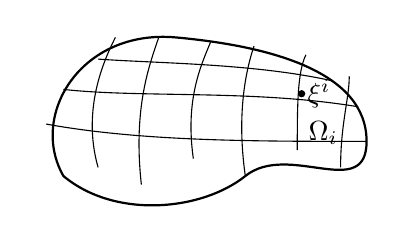
\begin{tikzpicture}[scale=1.1, >=stealth]
  \def\basepathB{
    (-1.4,-0.9) .. controls (-1.8,-0.2) and (-1.2,0.8) .. (-0.1,0.7)
    .. controls (1.0,0.6) and (2.1,0.3) .. (2.1,-0.5)
    .. controls (2.1,-1.2) and (1.2,-0.5) .. (0.7,-0.9)
    .. controls (0.2,-1.3) and (-0.8,-1.4) .. (-1.4,-0.9)
  }
  \draw[thick] \basepathB;

  % 内部网格线
  \draw (-1.0,-0.8) .. controls (-1.2,-0.1) and (-0.9,0.5) .. (-0.8,0.7);
  \draw (-0.5,-1.0) .. controls (-0.6,-0.1) and (-0.4,0.4) .. (-0.3,0.7);
  \draw (0.1,-0.7) .. controls (0.0,0.0) and (0.2,0.4) .. (0.3,0.65);
  \draw (0.7,-0.9) .. controls (0.6,-0.2) and (0.7,0.3) .. (0.8,0.6);
  \draw (1.3,-0.6) .. controls (1.3, -0.1) and (1.3,0.3) .. (1.4,0.5);
  \draw (1.8,-0.8) .. controls (1.8,-0.3) and (1.9,0.0) .. (1.9,0.25);

  \draw (-1.6,-0.3) .. controls (-0.5,-0.5) and (0.8,-0.5) .. (2.1,-0.5);
  \draw (-1.4,0.1) .. controls (-0.5,0.0) and (0.8,0.1) .. (2.0,-0.1);
  \draw (-1.0,0.45) .. controls (-0.3,0.4) and (0.8,0.4) .. (1.7,0.2);

  \node at (1.55, 0.05) {$\boldsymbol{\xi}^i$};
  \fill (1.35, 0.05) circle (1.2pt);
  \node at (1.6, -0.4) {$\Omega_i$};
\end{tikzpicture}
\caption{}\label{fig:10.1.2}
\end{minipage}
\end{figure}

对照一元函数积分的定义, 将 $[a, b]$ 分割成若干子区间, 计算这些区间的长度十分容易. 但是, 在 $\mathbb{R}^{2}$ 中, 一个点集 $\Omega$ 即使有界, 也可能相当复杂. 如何分割 $\Omega$, 如何确定面积 $v(\Omega_i)$, 这是建立二重积分精确定义的最大障碍. 为克服这些障碍, 我们分成两步: 首先讨论二维闭区间上的二重积分, 然后再讨论 $\mathbb{R}^{2}$ 中任一有界集上的二重积分.

\begin{definition}\label{def:10.1.1}
设 $I = [a, b] \times [c, d]$ 为 $\mathbb{R}^{2}$ 中的闭区间 (即每边平行于坐标轴的闭矩形 (闭长方形)). 作 $[a, b]$ 的分割
\[
  T_{x}\colon a = x_{0} < x_{1} < \cdots < x_{n} = b;
\]
又作 $[c, d]$ 的分割
\[
  T_{y}\colon c = y_{0} < y_{1} < \cdots < y_{m} = d.
\]
两族平行直线 $x = x_{i}\,(i = 0, 1, \cdots, n)$ 与 $y = y_{j}\,(j = 0, 1, \cdots, m)$ 将 $I$ 分割成 $k = n \times m$ 个子区间
\[
  [x_{i-1}, x_{i}] \times [y_{j-1}, y_{j}], \quad i = 1, \cdots, n;\; j = 1, \cdots, m.
\]
这 $k$ 个子区间的全体组成 $I$ 的一个分割 $T = T_x \times T_y = \{I_1, I_2, \cdots, I_k\}$. 任取 $\boldsymbol{\xi}^i \in I_i\, (i = 1, 2, \cdots, k)$. 对二元函数 $f\colon I \to \mathbb{R}$ 作 Riemann 和 (也称为积分和)
\[
  \sum_{i=1}^{k} f(\boldsymbol{\xi}^{i}) v(I_{i}),
\]
其中 $v(I_{i})$ 为二维闭区间 (闭矩形) $I_{i}$ 的面积, 即 $I_{i}$ 的长与宽之积. 记
\[
  \|T\| = \max\{\operatorname{diam}I_{1}, \operatorname{diam}I_{2}, \cdots, \operatorname{diam}I_{k}\},
\]
这里 $I_{i}$ 的直径 $\operatorname{diam}I_{i}$ 为矩形 $I_{i}$ 的对角线的长度. 称 $\|T\|$ 为分割 $T$ 的模或宽度. 称 $\boldsymbol{\xi} = (\boldsymbol{\xi}^{1}, \boldsymbol{\xi}^{2}, \cdots, \boldsymbol{\xi}^{k}) \in I_{1} \times I_{2} \times \cdots \times I_{k}$ 为上述 Riemann 和的值点向量, 称 $\boldsymbol{\xi}^{1}, \boldsymbol{\xi}^{2}, \cdots, \boldsymbol{\xi}^{k}$ 为值点.

如果 $\exists J \in \mathbb{R}$, s.t. $\forall \varepsilon > 0$, $\exists \delta > 0$, 当 $\|T\| < \delta$ 时, $\forall \boldsymbol{\xi} \in I_1 \times I_2 \times \cdots \times I_k$, 都有
\[
  \left|\sum_{i=1}^{k} f(\boldsymbol{\xi}^{i}) v(I_{i}) - J\right| < \varepsilon,
\]
则称二元函数 $f$ 在闭区间 $I$ 上 (Riemann) 可积, 而
\[
  J = \lim_{\|T\| \to 0} \sum_{i=1}^{k} f(\boldsymbol{\xi}^{i}) v(I_{i}) \reason{def} \iint_{I} f(x, y)\,\mathrm{d}x\mathrm{d}y \quad\text{或}\quad \int_{I} f\,\mathrm{d}v \quad\text{或}\quad \int_{I} f
\]
称为 $f$ 在 $I$ 上的二重积分, 或简称为 $f$ 在 $I$ 上的积分. 这里 $f$ 称为被积函数, $I$ 称为积分区间, $\mathrm{d}x\mathrm{d}y$ 与 $\mathrm{d}v$ 称为面积元.
\end{definition}

如此定义的积分具有与一元函数积分类似的简单性质.

\begin{theorem}\label{thm:10.1.1}
\begin{enumerate}
  \item $\displaystyle\int_{I} c = c v(I),\, c \in \mathbb{R}$;
  \item 设 $f$ 在二维闭区间 $I \subset \mathbb{R}^2$ 上可积, 则 $\forall c \in \mathbb{R}$ ($c$ 为常数), $cf$ 也可积, 且
  \[
    \int_{I} c f = c\int_{I} f.
  \]
  \item 设 $f_{1}$ 与 $f_{2}$ 在 $I$ 上都可积, 则 $f_{1} + f_{2}$ 在 $I$ 上也可积, 且
  \[
    \int_{I}(f_{1}+f_{2}) = \int_{I} f_{1} + \int_{I} f_{2}.
  \]
  \item 设 $f \geqslant 0$ 且在 $I$ 上可积, 则 $\displaystyle\int_{I} f \geqslant 0$. 特别地, 如果 $f_{1}, f_{2}$ 都在 $I$ 上可积, 且 $f_{1} \geqslant f_{2}$, 则 $\displaystyle\int_{I} f_{1} \geqslant \int_{I} f_{2}$.
  \item 设 $f$ 在 $I$ 上可积, 则 $|f|$ 在 $I$ 上也可积, 且
  \[
    \left|\int_{I} f\right| \leqslant \int_{I} |f|.
  \]
\end{enumerate}
\end{theorem}

\begin{proof}
(1) 因为
\[
  \sum_{i=1}^{k} c v(I_{i}) = c \sum_{i=1}^{k} v(I_{i}) = c v(I),
\]
所以根据积分定义知 $\displaystyle\int_{I} c = c v(I)$.

(2) 因为
\[
  \sum_{i=1}^{k} c f(\boldsymbol{\xi}^{i}) v(I_{i}) = c \sum_{i=1}^{k} f(\boldsymbol{\xi}^{i}) v(I_{i}),
\]
所以根据积分定义知 $\displaystyle\int_{I} c f = c\int_{I} f$.

(3) 因为
\[
  \sum_{i=1}^{k}(f_{1}+f_{2})(\boldsymbol{\xi}^{i}) v(I_{i}) = \sum_{i=1}^{k} f_{1}(\boldsymbol{\xi}^{i}) v(I_{i}) + \sum_{i=1}^{k} f_{2}(\boldsymbol{\xi}^{i}) v(I_{i}),
\]
所以根据积分定义知 $\displaystyle\int_{I}(f_{1}+f_{2}) = \int_{I} f_{1} + \int_{I} f_{2}$.

(4) 因为 $\displaystyle\sum_{i=1}^{k} f(\boldsymbol{\xi}^{i}) v(I_{i}) \geqslant 0$, 故必有 $\displaystyle\int_{I} f \geqslant 0$. (反证) 假设 $\displaystyle\int_{I} f < 0$, 取 $\varepsilon_{0} = -\dfrac{1}{2}\int_{I} f > 0$, 根据 $f$ 可积与积分定义知, $\exists \delta > 0$, 当 $\|T\| < \delta$ 时, 有
\[
  0 \leqslant \sum_{i=1}^{k} f(\boldsymbol{\xi}^{i}) v(I_{i}) < \int_{I} f + \varepsilon_{0} = \int_{I} f - \frac{1}{2}\int_{I} f = \frac{1}{2}\int_{I} f < 0,
\]
矛盾.

特别地, 当 $f_{1} \geqslant f_{2}$ 时, $f_{1} - f_{2} \geqslant 0$. 由上得到
\[
  \int_{I} f_{1} - \int_{I} f_{2} = \int_{I}(f_{1}-f_{2}) \geqslant 0 \implies \int_{I} f_{1} \geqslant \int_{I} f_{2}.
\]

(5) 类似\extref{例 6.1.9} 应用\cref{thm:10.1.7}的 (3) 或 (8) 知, $f$ 可积蕴涵着 $|f|$ 可积. 再由 $-|f| \leqslant f \leqslant |f|$ 及 (4) 立得
\[
  -\int_{I} |f| \leqslant \int_{I} f \leqslant \int_{I} |f|, \quad \text{即} \quad \left|\int_{I} f\right| \leqslant \int_{I} |f|. \qedhere
\]
\end{proof}

\begin{theorem}[惟一性]\label{thm:10.1.2}
设 $f$ 在闭区间 $I = [a, b] \times [c, d]$ 上可积, 则积分值 $J = \displaystyle\int_{I} f$ 是惟一的.
\end{theorem}

\begin{proof}
仿照\extref{定理 6.1.1}证明.
\end{proof}

\begin{theorem}[可积的必要条件]\label{thm:10.1.3}
设 $f$ 在闭区间 $I = [a, b] \times [c, d]$ 上可积, 则 $f$ 在 $I$ 上有界 (因而无界函数不是可积的). 但反之不真.
\end{theorem}

\begin{proof}
仿照\extref{定理 6.1.2}的证明. 只需将反例改为
\[
  f(x, y) = D(x, y) = \begin{cases}
    1, & (x, y) \in \mathbb{Q}^{2} \cap [0, 1]^{2}, \\
    0, & (x, y) \in [0, 1]^{2} \setminus \mathbb{Q}^{2}.
  \end{cases} \qedhere
\]
\end{proof}

与一元函数一样, \cref{thm:10.1.3}只是可积的必要条件, 它只能否定无界函数是可积的, 但对有界函数是否可积就束手无策了. 要判断一个函数是否可积, 原则上可以根据定义直接考察 Riemann 和是否无限接近某个常数 $J$. 但由于常数 $J$ 不易预知及 Riemann 和的复杂性, 这种判断是非常困难的.

为给出 $f$ 在 $I = [a, b] \times [c, d]$ 上可积的充要条件, 先引进零面积集、零测集的概念.

\begin{definition}\label{def:10.1.2}
设 $A \subset \mathbb{R}^{2}$. 如果对任何 $\varepsilon > 0$, 存在有限个闭区间 $I_{1}, I_{2}, \cdots, I_{k}$ 使得 $\bigcup\limits_{i=1}^{k} I_{i} \supseteq A$, 且 $\sum\limits_{i=1}^{k} v(I_{i}) < \varepsilon$, 则称 $A$ 为\textbf{零面积集}.

设 $A \subset \mathbb{R}^{2}$. 如果对任何 $\varepsilon > 0$, 存在至多可数个二维闭区间 $I_{1}, I_{2}, \cdots, I_{k}, \cdots$, 使得 $\bigcup\limits_{i=1}^{\infty} I_{i} \supseteq A$, 且 $\sum\limits_{i=1}^{\infty} v(I_{i}) < \varepsilon$, 则称 $A$ 为\textbf{零测集}.
\end{definition}

该定义中将「闭区间」改为「开区间」, 或「闭圆」, 或「开圆」都是等价的.

\begin{theorem}\label{thm:10.1.4}
零面积集必为零测集, 但反之不真.
\end{theorem}

\begin{proof}
如果 $A \subset \mathbb{R}^{2}$ 为零面积集, 则对任何 $\varepsilon > 0$, 必有二维闭区间 $I_{1}, I_{2}, \cdots, I_{k}$ 使 $\bigcup\limits_{i=1}^{k} I_{i} \supset A$, 且 $\sum\limits_{i=1}^{k} v(I_{i}) < \varepsilon$. 再选面积充分小的 $I_{k+1}, I_{k+2}, \cdots$, 使 $\sum\limits_{i=1}^{\infty} v(I_{i}) < \varepsilon$. 而 $\bigcup\limits_{i=1}^{\infty} I_{i} \supset \bigcup\limits_{i=1}^{k} I_{i} \supset A$ 是显然的. 因此, $A$ 为零测集.

\textbf{反例}: $[0, 1]^{2}$ 中有理点的全体 $\mathbb{Q}^{2} \cap [0, 1]^{2} = \{P^{i} \mid i \in \mathbb{Z}_{+}\}$ 为零测集, 但非零面积集. 作以 $P_i$ 为中心, $\dfrac{\sqrt{\varepsilon}}{2^i}$ 为边长的正方形 $I_i$, 则
\[
  \bigcup_{i=1}^{\infty} I_i \supset \bigcup_{i=1}^{\infty} \{P^i\} = \mathbb{Q}^{2} \cap [0, 1]^{2},
\]
且
\[
  \sum_{i=1}^{\infty} v(I_i) = \sum_{i=1}^{\infty} \left(\frac{\sqrt{\varepsilon}}{2^i}\right)^2 = \sum_{i=1}^{\infty} \frac{\varepsilon}{2^{2i}} = \sum_{i=1}^{\infty} \left(\frac{1}{4}\right)^i \varepsilon = \frac{\varepsilon}{3} < \varepsilon.
\]
由此推得 $\mathbb{Q}^{2} \cap [0, 1]^{2}$ 为零测集. 但它为非零面积集. (反证) 假设 $\mathbb{Q}^{2} \cap [0, 1]^{2}$ 为零面积集, 则对 $\varepsilon_0 = \dfrac{1}{2}$ 存在闭区间 $I_1, I_2, \cdots, I_k$ 使得 $\bigcup\limits_{i=1}^{k} I_i \supset \mathbb{Q}^{2} \cap [0, 1]^{2}$, 且 $\sum\limits_{i=1}^{k} v(I_i) < \varepsilon_0 = \dfrac{1}{2}$. 显然,
\[
  [0, 1]^{2} = \overline{\mathbb{Q}^{2} \cap [0, 1]^{2}} \subset \overline{\bigcup_{i=1}^{k} I_i} = \bigcup_{i=1}^{k} \overline{I_i} = \bigcup_{i=1}^{k} I_i,
\]
所以
\[
  1 = v([0, 1]^{2}) \leqslant v\left(\bigcup_{i=1}^{k} I_i\right) \leqslant \sum_{i=1}^{k} v(I_i) < \varepsilon_0 = \frac{1}{2},
\]
矛盾.
\end{proof}

\begin{example}\label{ex:10.1.1}
设 $f\colon [a, b] \to \mathbb{R}$ 为连续函数, 则集合 ($f$ 的图像)
\[
  \operatorname{graph} f = \{(x, f(x)) \mid x \in [a, b]\} \subset \mathbb{R}^{2}
\]
为零面积集.
\end{example}

\begin{proof}
任给 $\varepsilon > 0$, 因 $f$ 在 $[a, b]$ 上连续, 故一致连续. 于是, 存在 $[a, b]$ 的一个分割: $a = x_{0} < x_{1} < \cdots < x_{n} = b$, 当 $t_{1}, t_{2} \in [x_{i-1}, x_{i}]\, (i = 1, 2, \cdots, n)$ 时,
\[
  |f(t_{1}) - f(t_{2})| < \frac{\varepsilon}{b - a}.
\]
令 $m_{i} = \min f([x_{i-1}, x_{i}])$, $M_{i} = \max f([x_{i-1}, x_{i}])$, 则
\[
  0 \leqslant M_{i} - m_{i} < \frac{\varepsilon}{b - a}, \quad i = 1, 2, \cdots, n.
\]
设 $I_{i} = [x_{i-1}, x_{i}] \times [m_{i}, M_{i}]\, (i = 1, 2, \cdots, n)$. 显见 (\cref{fig:10.1.3}), $\operatorname{graph} f \subset \bigcup\limits_{i=1}^{n} I_{i}$, 且
\[
  \sum_{i=1}^{n} v(I_{i}) < \sum_{i=1}^{n}(x_{i} - x_{i-1}) \cdot \frac{\varepsilon}{b - a} = (b - a) \cdot \frac{\varepsilon}{b - a} = \varepsilon.
\]
因此, $\operatorname{graph} f$ 为零面积集.
\end{proof}

\begin{figure}[htbp]
\centering
\begin{tikzpicture}[scale=1.15, >=stealth]
  % 坐标轴
  \draw[->, thick] (-0.3,0) -- (6.0,0) node[below] {$x$};
  \draw[->, thick] (0,-0.3) -- (0,4.2) node[left] {$y$};

  % 各个竖直立柱的侧边界
  \draw[thick] (0.8,0) -- (0.8,2.0);
  \draw[thick] (1.7,0) -- (1.7,2.0);
  \draw[thick] (2.6,0) -- (2.6,2.2);
  \draw[thick] (3.5,0) -- (3.5,2.7);
  \draw[thick] (4.5,0) -- (4.5,3.6);
  \draw[thick] (5.4,0) -- (5.4,3.6);

  % 绘制每个柱体顶部的矩形 I_i [m_i, M_i] 并填充斜线阴影
  \fill[pattern=north east lines] (0.8,1.8) rectangle (1.7,2.0);
  \draw[thick] (0.8,1.8) rectangle (1.7,2.0);

  \fill[pattern=north east lines] (1.7,1.7) rectangle (2.6,1.9);
  \draw[thick] (1.7,1.7) rectangle (2.6,1.9);

  \fill[pattern=north east lines] (2.6,1.8) rectangle (3.5,2.2);
  \draw[thick] (2.6,1.8) rectangle (3.5,2.2);

  \fill[pattern=north east lines] (3.5,2.1) rectangle (4.5,2.7);
  \draw[thick] (3.5,2.1) rectangle (4.5,2.7);

  \fill[pattern=crosshatch] (4.5,2.6) rectangle (5.4,3.6);
  \draw[thick] (4.5,2.6) rectangle (5.4,3.6);

  % 函数曲线 y = f(x)
  \draw[very thick] (0.8,1.95) .. controls (1.2,1.82) and (1.5,1.75) .. (2.1,1.72)
    .. controls (2.6,1.75) and (3.0,1.95) .. (3.5,2.18)
    .. controls (4.0,2.4) and (4.3,2.6) .. (4.5,2.8)
    .. controls (4.8,3.1) and (5.2,3.4) .. (5.4,3.55);

  % 指向其中一个小矩形 I_i 的箭头
  \draw[->] (2.7, 3.2) node[above left] {$I_i$} -- (3.8, 2.5);
\end{tikzpicture}
\caption{}\label{fig:10.1.3}
\end{figure}

\begin{example}\label{ex:10.1.2}
设 $l \subset \mathbb{R}^{2}$ 为 $C^{1}$ 参数曲线, 则 $l$ 为零面积集.

更进一步, 设 $l \subset \mathbb{R}^{2}$ 为 $C^{0}$ 参数曲线, 并且其中至少有一个分量有连续的导数, 则 $l$ 为零面积集.
\end{example}

\begin{proof}
设 $l$ 有参数表示 $(x, y) = (x(t), y(t)),\, t \in [\alpha, \beta]$, 其中 $x$ 与 $y$ 为 $[\alpha, \beta]$ 上的连续函数, 不妨再设 $y$ 在 $[\alpha, \beta]$ 上有连续的导数. 由最值定理, $\exists M > 0$, s.t. $|y'(t)| \leqslant M$, $\forall t \in [\alpha, \beta]$. 于是, $\forall \varepsilon > 0$, 由于 $x(t)$ 在 $[\alpha, \beta]$ 上一致连续, 故必有分割
\[
  T\colon \alpha = t_{0} < t_{1} < \cdots < t_{m} = \beta,
\]
s.t. 当 $s, t \in [t_{i-1}, t_i]\, (i = 1, 2, \cdots, m)$ 时, 有
\[
  |x(s) - x(t)| < \frac{\varepsilon}{2M(\beta - \alpha)}.
\]
令
\[
  a_{i} = \min x([t_{i-1}, t_{i}]), \quad b_{i} = \max x([t_{i-1}, t_{i}]),
\]
则有 $b_{i} - a_{i} \leqslant \dfrac{\varepsilon}{2M(\beta - \alpha)}$. 再令
\[
  c_{i} = \min y([t_{i-1}, t_{i}]), \quad d_{i} = \max y([t_{i-1}, t_{i}]),
\]
\[
  I_{i} = [a_{i}, b_{i}] \times [c_{i}, d_{i}], \quad i = 1, 2, \cdots, m.
\]
于是, 当 $t \in [t_{i-1}, t_i]$ 时, $(x(t), y(t)) \in I_i\, (i = 1, 2, \cdots, m)$. 所以
\[
  l \subset \bigcup_{i=1}^{m} I_{i}.
\]
由于 $y(t)$ 在 $[\alpha, \beta]$ 上连续, 根据最值定理, $\exists t_{i}^{(0)}, t_{i}^{(1)} \in [t_{i-1}, t_{i}]$, s.t. $y(t_{i}^{(0)}) = d_{i}$, $y(t_{i}^{(1)}) = c_{i}$. 再由 Lagrange 中值定理, $\exists \theta_{i} \in [t_{i}^{(0)}, t_{i}^{(1)}] \subset [t_{i-1}, t_{i}]$, 有
\begin{align*}
  0 &\leqslant d_{i} - c_{i} = y(t_{i}^{(0)}) - y(t_{i}^{(1)}) = y'(\theta_{i})(t_{i}^{(0)} - t_{i}^{(1)}) \\
    &\leqslant M |t_{i}^{(0)} - t_{i}^{(1)}| \leqslant M(t_{i} - t_{i-1}).
\end{align*}
由此推得
\begin{align*}
  \sum_{i=1}^{m} v(I_{i}) &= \sum_{i=1}^{m}(b_{i} - a_{i})(d_{i} - c_{i}) \leqslant \sum_{i=1}^{m} \frac{\varepsilon}{2M(\beta - \alpha)} M(t_{i} - t_{i-1}) \\
  &= \frac{\varepsilon}{2M(\beta - \alpha)} M(\beta - \alpha) = \frac{\varepsilon}{2} < \varepsilon.
\end{align*}
这就证明了 $l$ 为零面积集.
\end{proof}

\begin{remark}\label{rem:10.1.1}
\begin{enumerate}
  \item 设函数 $f\colon [a, b] \to \mathbb{R}$ 连续, 由\cref{ex:10.1.2}的结论知, $f$ 的图像
  \[
    \operatorname{graph} f = \{(x, f(x)) \mid x \in [a, b]\} = \{(t, f(t)) \mid t \in [a, b]\} \subset \mathbb{R}^{2}
  \]
  为零面积集.
  \item 如果 $x(t), y(t)$ 只连续, 但都不具有连续可导的条件, 则\cref{ex:10.1.2}的结论可能不成立. 甚至我们将在第三册中给出一条连续的参数曲线, 它竟能充满整个正方形, 从而这条连续曲线就不是零面积集.
\end{enumerate}
\end{remark}

关于零面积集与零测集, 还有下面定理.

\begin{theorem}\label{thm:10.1.5}
\begin{enumerate}
  \item 至多可数集为零测集.
  \item 零测集的任何子集为零测集.
  \item 至多可数个零测集 $A_i$ 的并集 $\bigcup\limits_{i} A_i$ 仍为零测集.
  \item 零面积集的任何子集为零面积集.
  \item 有限个零面积集之并仍为零面积集; 可数个零面积集之并未必为零面积集.
  \item $A$ 为零面积集 $\iff \overline{A}$ 也为零面积集.
  \item 如果 $A$ 为有界闭集, 则 $A$ 为零测集 $\iff A$ 为零面积集.
\end{enumerate}
\end{theorem}

\begin{proof}
(1) $\sim$ (4) 和 (5) 的第一结论是显而易见的, 读者自己可以证明. 这里只证 (5) 的第二个论断及 (6), (7).

(5) $\boldsymbol{x} = (x, y) \in \mathbb{R}^{2}$, $\forall \varepsilon > 0$, 作闭区间
\[
  I = \left[x - \frac{\sqrt{\varepsilon}}{4}, x + \frac{\sqrt{\varepsilon}}{4}\right] \times \left[y - \frac{\sqrt{\varepsilon}}{4}, y + \frac{\sqrt{\varepsilon}}{4}\right],
\]
则 $\boldsymbol{x} \in I$, 且 $v(I) = \left(\dfrac{\sqrt{\varepsilon}}{2}\right)^{2} = \dfrac{\varepsilon}{4} < \varepsilon$. 因此, 独点集 $\{\boldsymbol{x}\}$ 为零面积集.

显然, $\mathbb{Q}^2 \cap [0, 1]^2 = \{P^i \mid i \in \mathbb{Z}_+\}$ 为可数个独点集之并, 因而它为可数个零面积集的并. 但根据\cref{thm:10.1.4}证明知, $\mathbb{Q}^2 \cap [0, 1]^2$ 为非零面积集.

(6) ($\Leftarrow$) 因为 $A \subset \overline{A}$, 根据 (4) 知, $\overline{A}$ 为零面积集蕴涵着 $A$ 为零面积集.

($\Rightarrow$) 设 $A$ 为零面积集, 则 $\forall \varepsilon > 0$, 必有闭区间 $I_{1}, I_{2}, \cdots, I_{m}$, s.t.
\[
  A \subset \bigcup_{i=1}^{m} I_{i}, \quad \sum_{i=1}^{m} v(I_{i}) < \varepsilon.
\]
由于 $\bigcup\limits_{i=1}^{m} I_{i}$ 为闭集, 所以仍有
\[
  \overline{A} \subset \overline{\bigcup_{i=1}^{m} I_{i}} = \bigcup_{i=1}^{m} \overline{I_{i}} = \bigcup_{i=1}^{m} I_{i}.
\]
由此可见 $\overline{A}$ 为零面积集.

(7) ($\Leftarrow$) 见\cref{thm:10.1.4}.

($\Rightarrow$) 设 $A$ 为紧致的零测集, 则对任何 $\varepsilon > 0$, 存在开区间序列 $\{I_{i}\}$, 使得
\[
  A \subset \bigcup_{i=1}^{\infty} I_{i} \quad\text{且}\quad \sum_{i=1}^{\infty} v(I_{i}) < \varepsilon.
\]
由有限覆盖定理, 从 $\{I_{i}\}$ 中可选出有限个开区间仍能覆盖住 $A$, 这些开区间面积之和自然仍小于 $\varepsilon$, 所以 $A$ 为零面积集.
\end{proof}

下面将给出 Riemann 可积的充要条件, 它只与被积函数 $f$ 本身有关, 而不涉及 Riemann 积分的值.

设 $f\colon I \to \mathbb{R}$ 为有界函数, $I = [a, b] \times [c, d] \subset \mathbb{R}^2$ 为闭区间, $M = \sup\limits_{\boldsymbol{x} \in I} f(\boldsymbol{x})$, $m = \inf\limits_{\boldsymbol{x} \in I} f(\boldsymbol{x})$. $T = \{I_1, I_2, \cdots, I_k\}$ 为\cref{def:10.1.1}中所述的 $I$ 的一个分割.
\[
  M_{i}^{f} = \sup_{\boldsymbol{x} \in I_{i}} f(\boldsymbol{x}), \quad m_{i}^{f} = \inf_{\boldsymbol{x} \in I_{i}} f(\boldsymbol{x}).
\]
在不致混淆时, 记 $M_{i}^{f}$ 为 $M_{i}$, $m_{i}^{f}$ 为 $m_{i}$.

分别称
\[
  S(T, f) = \sum_{i=1}^{k} M_{i} v(I_{i}) \quad\text{与}\quad s(T, f) = \sum_{i=1}^{k} m_{i} v(I_{i})
\]
为 $f$ 关于分割 $T$ 的 Darboux 上和与 Darboux 下和, 统称为 Darboux 和. 在不致混淆时, 分别记 $S(T, f)$ 与 $s(T, f)$ 为 $S(T)$ 与 $s(T)$. 显然, $\forall \boldsymbol{\xi}^{i} \in I_{i}\,(i = 1, 2, \cdots, k)$, Riemann 和 $S(T, f, \boldsymbol{\xi}) = \sum\limits_{i=1}^{k} f(\boldsymbol{\xi}^{i}) v(I_{i})$ 满足
\[
  m v(I) \leqslant \sum_{i=1}^{k} m_{i} v(I_{i}) \leqslant \sum_{i=1}^{k} f(\boldsymbol{\xi}^{i}) v(I_{i}) \leqslant \sum_{i=1}^{k} M_{i} v(I_{i}) \leqslant M v(I),
\]
即
\[
  m v(I) \leqslant s(T, f) \leqslant S(T, f, \boldsymbol{\xi}) \leqslant S(T, f) \leqslant M v(I),
\]
其中 $\boldsymbol{\xi} = (\boldsymbol{\xi}^{1}, \boldsymbol{\xi}^{2}, \cdots, \boldsymbol{\xi}^{k})$.

设 $\omega_{i}^{f} = M_{i}^{f} - m_{i}^{f}$, 称它为 $f$ 在 $I_{i}$ 上的振幅, 简记为 $\omega_{i} = M_{i} - m_{i}$, 而
\[
  S(T, f) - s(T, f) = \sum_{i=1}^{k}(M_{i} - m_{i}) v(I_{i}) = \sum_{i=1}^{k} \omega_{i} v(I_{i}) \quad \left(\text{或}\quad \sum_{T} \omega_{i} v(I_{i})\right)
\]
称为 $f$ 在 $I$ 上关于分割 $T$ 的振幅和.

\begin{lemma}\label{lem:10.1.1}
对闭区间 $I \subset \mathbb{R}^2$ 的同一分割 $T = \{I_1, I_2, \cdots, I_k\}$, 相对于任何 $\boldsymbol{\xi} = (\boldsymbol{\xi}^1, \boldsymbol{\xi}^2, \cdots, \boldsymbol{\xi}^k) \in I_1 \times I_2 \times \cdots \times I_k$, 有
\[
  S(T, f) = \sup_{\boldsymbol{\xi}} \sum_{i=1}^{k} f(\boldsymbol{\xi}^{i}) v(I_{i}), \quad s(T, f) = \inf_{\boldsymbol{\xi}} \sum_{i=1}^{k} f(\boldsymbol{\xi}^{i}) v(I_{i}).
\]
\end{lemma}

\begin{proof}
仿\extref{引理 6.1.1}证明.
\end{proof}

设 $T' = T_{x}' \times T_{y}'$, $T'' = T_{x}'' \times T_{y}''$ 为闭区间 $I \subset \mathbb{R}^2$ 的两个分割. $T_{x}' + T_{x}''$ 表示将 $T'_{x}$ 与 $T''_{x}$ 的所有分点合并得到的分割 (重复的分点只取一次), $T'_{y} + T''_{y}$ 表示将 $T'_{y}$ 与 $T''_{y}$ 的所有分点合并得到的分割 (重复的分点只取一次). 记 $T' + T'' = (T_{x}' + T''_{x}) \times (T'_{y} + T''_{y})$.

\begin{lemma}\label{lem:10.1.2}
$S(T' + T'') \leqslant S(T')$, $s(T' + T'') \geqslant s(T')$;
\[
  S(T' + T'') \leqslant S(T''), \quad s(T' + T'') \geqslant s(T'').
\]
\end{lemma}

\begin{proof}
类似\extref{引理 6.1.2}的证明知, 分割增加新分点后, 上和不增, 下和不减. 因此, 立即推得引理中的结论.
\end{proof}

\begin{lemma}\label{lem:10.1.3}
对闭区间 $I \subset \mathbb{R}^{2}$ 的任意两个分割 $T'$ 与 $T''$, 有
\[
  s(T') \leqslant S(T'').
\]
\end{lemma}

\begin{proof}
由\cref{lem:10.1.2}便有
\[
  s(T') \leqslant s(T' + T'') \leqslant S(T' + T'') \leqslant S(T''). \qedhere
\]
\end{proof}

\begin{lemma}\label{lem:10.1.4}
$m v(I) \leqslant \sup\limits_{T'} s(T') \leqslant \inf\limits_{T''} S(T'') \leqslant M v(I)$.
\end{lemma}

\begin{proof}
由\cref{lem:10.1.3}知
\[
  m v(I) \leqslant s(T') \leqslant S(T'') \leqslant M v(I),
\]
从而有
\[
  m v(I) \leqslant \sup_{T'} s(T') \leqslant \inf_{T''} S(T'') \leqslant M v(I),
\]
即
\[
  m v(I) \leqslant s \leqslant S \leqslant M v(I),
\]
其中 $S = \inf\limits_{T} S(T)$ 与 $s = \sup\limits_{T} s(T)$ 分别称为 $f$ 在 $I$ 上的上积分与下积分.
\end{proof}

\begin{theorem}[Darboux 定理]\label{thm:10.1.6}
$\lim\limits_{\|T\| \to 0} S(T) = S, \quad \lim\limits_{\|T\| \to 0} s(T) = s$.
\end{theorem}

\begin{proof}
$\forall \varepsilon > 0$, 由 $S$ 的定义知, 必有某个分割 $T' = T_{x}' \times T_{y}'$, s.t.
\[
  S(T') < S + \frac{\varepsilon}{2}.
\]
设 $T_{x}'$ 与 $T_{y}'$ 分别由 $p$ 个与 $q$ 个分点构成. 对于任意另外一个分割 $T$, $(T+T')_{x}$ 至多比 $T_{x}$ 多 $p$ 个分点, $(T+T')_{y}$ 至多比 $T_{y}$ 多 $q$ 个分点. 根据\extref{引理 6.1.2}证明中的方法与\cref{lem:10.1.2}有
\begin{align*}
  S(T) - (M - m)[p(d - c) + q(b - a)] \|T\|
  &\leqslant S(T) - (M - m)[p(d - c)\|T_{x}\| + q(b - a)\|T_{y}\|] \\
  &\leqslant S(T + T') \leqslant S(T').
\end{align*}
于是, 当 $\|T\| < \dfrac{\varepsilon}{2(M - m + 1)[p(d - c) + q(b - a)]}$ 时,
\begin{align*}
  S &\leqslant S(T) \leqslant S(T') + (M - m)[p(d - c) + q(b - a)] \|T\| \\
    &< S(T') + (M - m)[p(d - c) + q(b - a)] \frac{\varepsilon}{2(M - m + 1)[p(d - c) + q(b - a)]} \\
    &< S(T') + \frac{\varepsilon}{2} < \left(S + \frac{\varepsilon}{2}\right) + \frac{\varepsilon}{2} = S + \varepsilon.
\end{align*}
这就证明了 $\lim\limits_{\|T\| \to 0} S(T) = S$.

同理, 或用 $-f$ 代替 $f$ 得到 $\lim\limits_{\|T\| \to 0} s(T) = s$.
\end{proof}

\begin{theorem}[Riemann 可积的充要条件]\label{thm:10.1.7}
设 $I \subset \mathbb{R}^2$ 为闭区间, $f\colon I \to \mathbb{R}$ 为有界函数, 即 $|f(\boldsymbol{x})| \leqslant M$, $\forall \boldsymbol{x} \in I$. 则下面结论等价:
\begin{enumerate}
  \item $f$ 在 $I$ 上 Riemann 可积.
  \item $f$ 在 $I$ 上的上积分与下积分相等, 即 $S = s$.
  \item 对任何 $\varepsilon > 0$, 存在 $I$ 的某个分割 $T$, 使得
  \[
    S(T) - s(T) = \sum_{i=1}^{k} \omega_{i} v(I_{i}) < \varepsilon.
  \]
  \item 存在 $I$ 的分割串 $T_{m}\,(m = 1, 2, \cdots)$, 使得
  \[
    \lim_{m \to +\infty}[S(T_{m}) - s(T_{m})] = 0.
  \]
  \item $\lim\limits_{\|T\| \to 0}[S(T) - s(T)] = 0$.
  \item 对任何 $\varepsilon > 0$, 存在 $I$ 的某个分割 $T$, 使对任何 $\boldsymbol{\xi} = (\boldsymbol{\xi}^{1}, \boldsymbol{\xi}^{2}, \cdots, \boldsymbol{\xi}^{k}) \in I_{1} \times I_{2} \times \cdots \times I_{k}$, 有
  \[
    |S(T, f, \boldsymbol{\xi}) - J| < \varepsilon.
  \]
  \item 对任何 $\varepsilon > 0, \eta > 0$, 存在 $I$ 的某个分割 $T = \{I_{1}, I_{2}, \cdots, I_{k}\}$, 使得
  \[
    \sum_{\omega_{i} \geqslant \varepsilon} v(I_{i}) < \eta.
  \]
  \item \textbf{(Lebesgue 定理)} $f$ 在 $I$ 上几乎处处连续, 即 $f$ 的不连续点集 $D_{\text{不}}^{f}$ (简记为 $D_{\text{不}}$) 为零测集, 记作
  \[
    \operatorname{meas} D_{\text{不}} = 0.
  \]
\end{enumerate}
\end{theorem}

\begin{proof}
我们只证 (3) $\Leftrightarrow$ (8), 其余证明完全仿照\extref{定理 6.1.4}中相应部分的证明.

(3) $\Rightarrow$ (8): 对任何 $\varepsilon > 0$, 存在 $I$ 的某分割 $T = \{I_{1}, I_{2}, \cdots, I_{k}\}$, 使得
\[
  S(T) - s(T) < \frac{\delta}{2} \varepsilon,
\]
其中 $\delta > 0$ 为任何正数. 令
\[
  D_{\delta} = \left\{\boldsymbol{x} \in I \;\middle|\; \omega_{f}(\boldsymbol{x}) = \lim_{r \to 0^{+}} \omega_{f}(\boldsymbol{x}, r) = \lim_{r \to 0^{+}} [\sup f(I \cap B(\boldsymbol{x}; r)) - \inf f(I \cap B(\boldsymbol{x}; r))] \geqslant \delta\right\},
\]
则
\[
  \sum_{D_{\delta} \cap I_{i}^{\circ} \neq \varnothing} v(I_{i}) < \frac{\varepsilon}{2}.
\]
若不然,
\[
  \frac{\delta}{2}\varepsilon > S(T) - s(T) \geqslant \sum_{D_{\delta} \cap I_{i}^{\circ} \neq \varnothing} \omega_{i} v(I_{i}) \geqslant \sum_{D_{\delta} \cap I_{i}^{\circ} \neq \varnothing} \delta v(I_{i}) \geqslant \delta \cdot \frac{\varepsilon}{2} = \frac{\delta}{2}\varepsilon,
\]
矛盾.

显然, $\bigcup\limits_{i=1}^{k} \partial I_{i}$ 为零面积集, 故必有闭区间 $J_{1}, J_{2}, \cdots, J_{m}$, 使得
\[
  \bigcup_{i=1}^{k} \partial I_{i} \subset \bigcup_{j=1}^{m} J_{j}, \quad\text{且}\quad \sum_{j=1}^{m} v(J_{j}) < \frac{\varepsilon}{2}.
\]
由此可知
\[
  D_{\delta} \subset \left(\bigcup_{\omega_{i} \geqslant \delta} I_{i}\right) \bigcup \left(\bigcup_{j=1}^{m} J_{j}\right),
\]
并且
\[
  \sum_{\omega_{i} \geqslant \delta} v(I_{i}) + \sum_{j=1}^{m} v(J_{j}) < \frac{\varepsilon}{2} + \frac{\varepsilon}{2} = \varepsilon.
\]
这就证明了 $D_{\delta}$ 为零测集, 从而由下面的\cref{thm:10.1.8}与\cref{thm:10.1.5}(3) 知, $D_{\text{不}} = \bigcup\limits_{n=1}^{\infty} D_{\frac{1}{n}}$ 为零测集.

(8) $\Rightarrow$ (3): 设 $D_{\text{不}}$ 为零测集. $\forall \varepsilon > 0$, 存在开区间序列 $\{U_{i}\}$, 使得
\[
  D_{\text{不}} \subset \bigcup_{i=1}^{\infty} U_{i}, \quad \sum_{i=1}^{\infty} v(U_{i}) < \frac{\varepsilon}{4M + 1}.
\]
对任何 $\boldsymbol{x} \in I \setminus \bigcup\limits_{i=1}^{\infty} U_{i} \subset I \setminus D_{\text{不}}$, $f$ 在 $\boldsymbol{x}$ 处连续, 故存在 $\boldsymbol{x}$ 的开邻域 $U_{\boldsymbol{x}}$, 使得 $\omega_{f}(U_{\boldsymbol{x}} \cap I) < \dfrac{\varepsilon}{2 v(I)}$.

显然 $\mathcal{J} = \left\{U_{i}, U_{\boldsymbol{x}} \;\middle|\; i = 1, 2, \cdots;\; \boldsymbol{x} \in I \setminus \bigcup\limits_{i=1}^{\infty} U_{i}\right\}$ 为紧致集 $I$ 的一个开覆盖. 根据 Heine-Borel 有限覆盖定理, 存在 $\mathcal{J}$ 的有限子集 $\mathcal{J}' = \{U_{i_{l}}, U_{\boldsymbol{x}^{s}} \mid l = 1, 2, \cdots, p;\; s = 1, 2, \cdots, q\}$ 覆盖 $I$. 再根据 Lebesgue 数定理, 存在 Lebesgue 数 $\lambda = \lambda(\mathcal{J}') > 0$. 当 $I$ 的分割 $T = \{I_{1}, I_{2}, \cdots, I_{k}\}$ 满足 $\|T\| < \lambda$ 时, 必有
\[
  I_{i} \subset U_{i_{l}} \quad\text{或}\quad U_{\boldsymbol{x}^{s}}.
\]
于是
\begin{align*}
  0 &\leqslant S(T) - s(T) = \sum_{i=1}^{k} \omega_{i} v(I_{i}) \\
    &\leqslant \sum_{I_{i} \subset U_{i_{l}}} \omega_{i} v(I_{i}) + \sum_{I_{i} \subset U_{\boldsymbol{x}^{s}}} \omega_{i} v(I_{i}) \\
    &\leqslant 2M \sum_{1} v(I_{i}) + \frac{\varepsilon}{2 v(I)} \sum_{2} v(I_{i}) \\
    &\leqslant 2M \sum_{i=1}^{\infty} v(U_{i}) + \frac{\varepsilon}{2 v(I)} v(I) \\
    &< 2M \cdot \frac{\varepsilon}{4M + 1} + \frac{\varepsilon}{2} < \varepsilon. \qedhere
\end{align*}
\end{proof}

\begin{remark}\label{rem:10.1.2}
我们可以不应用 Darboux 定理证明\cref{thm:10.1.7}中的 (2) $\Rightarrow$ (3).

事实上, 设 $J = S = s$. 由下积分的定义, 对任何 $\varepsilon > 0$, 存在闭区间 $I$ 的一个分割 $T'$, 使得
\[
  s(T') > J - \frac{\varepsilon}{2};
\]
又由上积分的定义, 存在闭区间 $I$ 的一个分割 $T''$, 使得
\[
  S(T'') < J + \frac{\varepsilon}{2}.
\]
于是, 有
\[
  J - \frac{\varepsilon}{2} < s(T') \leqslant s(T' + T'') \leqslant S(T' + T'') \leqslant S(T'') < J + \frac{\varepsilon}{2}.
\]
由此推得
\[
  S(T' + T'') - s(T' + T'') < \left(J + \frac{\varepsilon}{2}\right) - \left(J - \frac{\varepsilon}{2}\right) = \varepsilon.
\]
令 $T = T' + T''$, 它为 $I$ 的一个分割, 且有
\[
  S(T) - s(T) < \varepsilon.
\]
\end{remark}

\begin{theorem}\label{thm:10.1.8}
设 $A \subset \mathbb{R}^{2}$, 则
\[
  \text{函数 } f\colon A \to \mathbb{R} \text{ 在点 } \boldsymbol{x} \in A \text{ 处连续} \iff \omega_f(\boldsymbol{x}) = \lim_{r \to 0^+} \omega_f(\boldsymbol{x}, r) = 0,
\]
其中 $\omega_{f}(\boldsymbol{x}, r) = \sup f(A \cap B(\boldsymbol{x}; r)) - \inf f(A \cap B(\boldsymbol{x}; r))$ 为 $f$ 在 $A \cap B(\boldsymbol{x}; r)$ 上的振幅, 而 $\omega_{f}(\boldsymbol{x})$ 为 $f$ 在点 $\boldsymbol{x}$ 处的振幅.
\end{theorem}

\begin{proof}
与\extref{定理 2.4.6}的证明完全类似.
\end{proof}

\begin{example}\label{ex:10.1.3}
证明 Dirichlet 函数
\[
  D(x, y) = \begin{cases}
    1, & (x, y) \in \mathbb{Q}^{2} \cap [0, 1]^{2}, \\
    0, & (x, y) \in [0, 1]^{2} \setminus \mathbb{Q}^{2}
  \end{cases}
\]
在 $[0, 1]^{2}$ 上不可积.
\end{example}

\begin{proof}
\textbf{证法 1}\quad 类似\extref{定理 6.1.2}中反例的证明.

\textbf{证法 2, 3, 4}\quad 类似\extref{例 6.1.1}中的证法 2, 3, 4.
\end{proof}

\begin{example}\label{ex:10.1.4}
设 $I \subset \mathbb{R}^2$ 为闭区间, $f\colon I \to \mathbb{R}$ 有界. 若 $l = \{\boldsymbol{x} \in I \mid f(\boldsymbol{x}) \neq 0\}$ 为零面积集, 则 $f$ 在 $I$ 上可积, 且 $\displaystyle\int_I f = 0$.
\end{example}

\begin{proof}
\textbf{证法 1}\quad 显然, $I^{\circ} \setminus \overline{l} = I^{\circ} \cap (\mathbb{R}^{2} \setminus \overline{l})$ 中的点为 $f$ 的连续点, 可见 $D_{\text{不}} \subset \partial I \cup \overline{l}$. 由于 $\partial I$ 与 $\overline{l}$ 都为零面积集, 故 $\partial I \cup \overline{l}$ 也为零面积集. 根据 Lebesgue 定理 (\cref{thm:10.1.7}(8)) 知, $f$ 在 $I$ 上可积.

对于 $I$ 的任一分割 $T = \{I_{1}, I_{2}, \cdots, I_{k}\}$. 由于 $\overline{l}$ 为零面积集, 故必 $\exists \boldsymbol{\xi}^{i} \in I_{i}$, s.t. $f(\boldsymbol{\xi}^{i}) = 0\,(i = 1, 2, \cdots, k)$. 此时, Riemann 和
\[
  \sum_{i=1}^{k} f(\boldsymbol{\xi}^{i}) v(I_{i}) = 0.
\]
由积分的存在性立知 $\displaystyle\int_{I} f = 0$.

\textbf{证法 2}\quad 设 $|f(\boldsymbol{x})| < M$, $\forall \boldsymbol{x} \in I$. $\forall \varepsilon > 0$, 因为 $l$ 为零面积集, 故存在闭区间 $J_{1}, J_{2}, \cdots, J_{m}$, 使 $\bigcup\limits_{i=1}^{m} J_{i} \supset l$, 且 $\sum\limits_{i=1}^{m} v(J_{i}) < \dfrac{\varepsilon}{M}$. 将每个 $J_{i}$ 稍稍扩大得到闭区间 $\widetilde{J}_{i}$, 使 $\sum\limits_{i=1}^{m} v(\widetilde{J}_{i}) < \dfrac{\varepsilon}{M}$, 且
\[
  \delta = \rho_{0}^{2}\left(l, \partial\left(\bigcup_{i=1}^{m}\widetilde{J}_{i}\right)\right) = \inf\left\{\rho_{0}^{2}(\boldsymbol{x}, \boldsymbol{y}) = \|\boldsymbol{x} - \boldsymbol{y}\| \;\middle|\; \boldsymbol{x} \in l, \boldsymbol{y} \in \partial\left(\bigcup_{i=1}^{m}\widetilde{J}_{i}\right)\right\} > 0.
\]
设 $T = \{I_{1}, I_{2}, \cdots, I_{k}\}$ 为 $I$ 的一个分割, 且 $\|T\| < \delta$, 则当 $I_{j} \cap l \neq \varnothing$ 时, 必有 $I_{j} \subset \bigcup\limits_{i=1}^{m} \widetilde{J}_{i}$, 所以
\begin{align*}
  |S(T, f, \boldsymbol{\xi}) - 0| &= \left|\sum_{I_{j} \cap l \neq \varnothing} f(\boldsymbol{\xi}^{j}) v(I_{j}) + \sum_{I_{j} \cap l = \varnothing} f(\boldsymbol{\xi}^{j}) v(I_{j})\right| \\
  &= \left|\sum_{I_{j} \cap l \neq \varnothing} f(\boldsymbol{\xi}^{j}) v(I_{j})\right| \leqslant M \sum_{I_{j} \cap l \neq \varnothing} v(I_{j}) \leqslant M \sum_{i=1}^{m} v(\widetilde{J}_{i}) \\
  &< M \cdot \frac{\varepsilon}{M} = \varepsilon,
\end{align*}
从而 $\displaystyle\int_{I} f = \lim_{\|T\| \to 0} S(T, f, \boldsymbol{\xi}) = 0$.
\end{proof}

\begin{remark}\label{rem:10.1.3}
\begin{enumerate}
  \item 从\cref{ex:10.1.4}可知, $\mathbb{Q}^{2} \cap [0, 1]^{2}$ 不为零面积集.
  
  (反证) 假设 $\mathbb{Q}^{2} \cap [0, 1]^{2}$ 为零面积集, 则由\cref{ex:10.1.4}推得 $\mathbb{Q}^{2} \cap [0, 1]^{2}$ 的特征函数, 即 Dirichlet 函数
  \[
    \chi_{\mathbb{Q}^{2} \cap [0, 1]^{2}}(x, y) = D(x, y) = \begin{cases}
      1, & (x, y) \in \mathbb{Q}^{2} \cap [0, 1]^{2}, \\
      0, & (x, y) \in [0, 1]^{2} \setminus \mathbb{Q}^{2}
    \end{cases}
  \]
  在 $[0, 1]^{2}$ 上可积, 且积分为 0. 这与\cref{thm:10.1.3}中的反例 $D(x, y)$ 在 $[0, 1]^{2}$ 上不可积相矛盾.
  \item \cref{ex:10.1.4}中, 将「$l$ 为零面积集」改为「$l$ 为零测集」结论不真. 上述 $D(x, y)$ 就是反例.
\end{enumerate}
\end{remark}

\begin{example}\label{ex:10.1.5}
设 $I \subset \mathbb{R}^2$ 为闭区间, $f, g\colon I \to \mathbb{R}$ 都为有界函数, 集合 $l = \{\boldsymbol{x} \in I \mid f(\boldsymbol{x}) \neq g(\boldsymbol{x})\}$ 为一零面积集. 如果 $f$ 与 $g$ 中有一个在 $I$ 上可积, 则另一个也在 $I$ 上可积, 并且
\[
  \int_{I} f = \int_{I} g.
\]
\end{example}

\begin{proof}
不妨设 $g$ 在 $I$ 上可积. 由于有界函数 $f - g$ 具有性质: $l = \{\boldsymbol{x} \in I \mid f(\boldsymbol{x}) - g(\boldsymbol{x}) \neq 0\}$ 为零面积集, 根据\cref{ex:10.1.4}的结果, $f - g$ 在 $I$ 上可积, 且
\[
  \int_{I}(f - g) = 0.
\]
再根据\cref{thm:10.1.1}, 有
\[
  \int_{I} f = \int_{I}[(f - g) + g] = \int_{I}(f - g) + \int_{I} g = 0 + \int_{I} g = \int_{I} g. \qedhere
\]
\end{proof}

从\cref{ex:10.1.5}中可知, 若函数 $f$ 在闭区间 $I$ 上有界, 只在一个零面积集上改变 $f$ 的值, 但仍使之保持有界, 那么既不会改变函数的可积性, 也不会改变其积分值.

\begin{example}\label{ex:10.1.6}
设 $I \subset \mathbb{R}^{2}$ 为闭区间, $A \subset I$, $A$ 的特征函数
\[
  \chi_{A}(\boldsymbol{x}) = \begin{cases}
    1, & \boldsymbol{x} \in A, \\
    0, & \boldsymbol{x} \in I \setminus A,
  \end{cases}
\]
则
\[
  A = \{\boldsymbol{x} \in I \mid \chi_A(\boldsymbol{x}) \neq 0\} \text{ 为零面积集} \iff \int_I \chi_A = 0.
\]
\end{example}

\begin{proof}
($\Rightarrow$) 因 $A = \{\boldsymbol{x} \in I \mid \chi_{A}(\boldsymbol{x}) \neq 0\}$ 为零面积集, 故根据\cref{ex:10.1.4}知, $\displaystyle\int_{I} \chi_{A} = 0$.

($\Leftarrow$) 设 $\displaystyle\int_{I} \chi_{A} = 0$. $\forall \varepsilon > 0$, $\exists \delta > 0$, 对 $I$ 的分割 $T = \{I_{1}, I_{2}, \cdots, I_{k}\}$, 当 $\|T\| < \delta$ 时, 有
\[
  0 \leqslant S(T, \chi_{A}, \boldsymbol{\xi}) = \sum_{i=1}^{k} \chi_{A}(\boldsymbol{\xi}^{i}) v(I_{i}) < \varepsilon, \quad \forall \boldsymbol{\xi} = (\boldsymbol{\xi}^{1}, \boldsymbol{\xi}^{2}, \cdots, \boldsymbol{\xi}^{k}) \in I_{1} \times I_{2} \times \cdots \times I_{k}.
\]
当 $A \cap I_i \neq \varnothing$ 时, 取 $\boldsymbol{\xi}^i \in A \cap I_i$, 则
\[
  0 \leqslant \sum_{A \cap I_{i} \neq \varnothing} \chi_{A}(\boldsymbol{\xi}^{i}) v(I_{i}) = \sum_{A \cap I_{i} \neq \varnothing} v(I_{i}) < \varepsilon,
\]
且 $\bigcup\limits_{A \cap I_{i} \neq \varnothing} I_{i} \supseteq A$, 所以 $A$ 为零面积集.
\end{proof}

\begin{example}\label{ex:10.1.7}
证明: 函数
\[
  f(x, y) = \sin\frac{1}{(x^{2}-1)^{2}+(y^{2}-1)^{2}}
\]
在闭区间 $[-2, 2]^{2}$ 上可积.
\end{example}

\begin{proof}
函数 $f$ 在 $[-2, 2]^{2}$ 中的 4 个点 $(-1, -1), (-1, 1), (1, -1), (1, 1)$ 上无定义. 但这 4 个点组成的集合为零面积集. 补充定义 $f$ 在这 4 个点之值 (可以为任何实常数), $f$ 在 $[-2, 2]^{2}$ 上是有界的, 其不连续点集为上述 4 个点, 它是零面积集, 当然是零测集, 根据\cref{thm:10.1.7}(8) 知, $f$ 在 $[-2, 2]^{2}$ 上是可积的.
\end{proof}

\begin{example}\label{ex:10.1.8}
证明: 函数
\[
  f(x, y) = \arctan\frac{1}{y - x^{2}}
\]
在闭区间 $[0, 1]^{2}$ 上可积.
\end{example}

\begin{proof}
函数 $f$ 在抛物线的一段 $l = \{(x, x^{2}) \mid 0 \leqslant x \leqslant 1\}$ 上无定义. 由\cref{ex:10.1.2}知 $l$ 为零面积集. 我们可以在 $l$ 上为 $f$ 赋以实数值, 使 $f$ 在 $[0, 1]^{2}$ 上保持有界, 则 $f$ 在 $[0, 1]^{2}$ 上的不连续点集为 $l$, 它是零面积集, 当然是零测集, 根据\cref{thm:10.1.7}(8) 知, $f$ 在 $[0, 1]^{2}$ 上是可积的.
\end{proof}

\begin{exblock}{练习题 10.1}
1. 设 $a > 0$, 根据二重积分的定义及对称性证明
\[
  \iint\limits_{[-a, a]^{2}} \sin(x+y)\,\mathrm{d}x\mathrm{d}y = 0,
\]
并从几何上说明这一结果.

2. 设一元函数 $f, g$ 在区间 $[0, 1]$ 上可积. 应用二重积分定义证明: 二元函数 $f(x)g(y)$ 在 $[0, 1]^{2}$ 上也可积, 并且
\[
  \iint\limits_{[0, 1]^{2}} f(x)g(y)\,\mathrm{d}x\mathrm{d}y = \int_{0}^{1} f(x)\,\mathrm{d}x \int_{0}^{1} g(y)\,\mathrm{d}y.
\]
试应用另外的方法证明 $f(x)g(y)$ 在 $[0, 1]^{2}$ 上可积, 再由定理 10.3.3 证明上述公式.

3. 计算二重积分:

\begin{tabular}{@{}p{0.46\linewidth}p{0.50\linewidth}@{}}
(1) $\displaystyle\iint\limits_{[0, 1]^{2}} \mathrm{e}^{x+y}\,\mathrm{d}x\mathrm{d}y$; & (2) $\displaystyle\iint\limits_{x^{2}+y^{2} \leqslant 4} \operatorname{sgn}(x^{2}-y^{2}+2)\,\mathrm{d}x\mathrm{d}y$.
\end{tabular}

4. 设点列 $\{\boldsymbol{x}^n\}$ 在 $\mathbb{R}^2$ 中有极限. 证明: 集合 $\{\boldsymbol{x}^n \mid n \in \mathbb{Z}_+\}$ 为一零面积集.

5. 设 $A \subset \mathbb{R}^{2}$ 为有界集, 且 $A$ 的导集 $A'$ 为零面积集, 证明 $\overline{A}$ 也是零面积集.

6. 设 $J$ 与 $I$ 均为闭区间, $J \subset I$, 且 $f$ 在 $I$ 上可积, 证明: $f$ 在 $J$ 上也可积.

7. 研究 $[0, 1]^{2}$ 上的二元函数
\[
  f(x, y) = \begin{cases}
    \sin\dfrac{1}{xy}, & x \neq 0 \text{ 且 } y \neq 0, \\
    0, & x = 0 \text{ 或 } y = 0
  \end{cases}
\]
的可积性.

8. 设 $I$ 为 $\mathbb{R}^2$ 中的一个有界闭区间, $A = \{\boldsymbol{x}^1, \boldsymbol{x}^2, \cdots, \boldsymbol{x}^n, \cdots\} \subset I$. 定义二元函数
\[
  f(\boldsymbol{x}) = \begin{cases}
    \dfrac{1}{n}, & \boldsymbol{x} = \boldsymbol{x}^{n},\, n \in \mathbb{Z}_{+}, \\
    0, & \boldsymbol{x} \notin A.
  \end{cases}
\]
研究二元函数 $f$ 在 $I$ 上的可积性.

9. 设二元函数 $f$ 与 $g$ 在闭区间 $I \subset \mathbb{R}^{2}$ 上可积. 证明: $fg$ 在 $I$ 上也可积. 问: 当 $g$ 在 $I$ 上不取零值时, $\dfrac{f}{g}$ 也在 $I$ 上可积吗? 说明理由.
\end{exblock}

\begin{exblock}{思考题 10.1}
1. 设 $f > 0$ 在闭区间 $I \subset \mathbb{R}^{2}$ 上成立, 且 $f$ 在 $I$ 可积, 证明: $\displaystyle\int_{I} f > 0$.

2. 设闭区间 $I \subset \mathbb{R}^2$ 上的连续函数列 $\{f_n\}$ 满足 $f_1 \geqslant f_2 \geqslant \cdots \geqslant f_n \geqslant \cdots$, 且 $\lim\limits_{n \to +\infty} f_n = 0$. 证明:
\begin{enumerate}
  \item $f_n$ 在 $I$ 上一致收敛于 0;
  \item $\lim\limits_{n \to +\infty} \displaystyle\int_{I} f_n = 0$.
\end{enumerate}

3. 设 $I \subset \mathbb{R}^{2}$ 为闭区间, 且 $\displaystyle\int_{I} f > 0$. 证明: 存在闭区间 $J \subset I$, 使得 $f > 0$ 在 $J$ 上成立.

4. (1) 设 $f(x)$ 在 $[a, b]$ 上连续. 应用二重积分性质与 $f(x)f(y) \leqslant \dfrac{f^{2}(x)+f^{2}(y)}{2}$ 证明:
\[
  \left[\int_{a}^{b} f(x)\,\mathrm{d}x\right]^{2} \leqslant (b-a)\int_{a}^{b} f^{2}(x)\,\mathrm{d}x,
\]
其中等号仅在 $f(x)$ 为常值函数时成立.

(2) 设 $f(x)$ 与 $g(x)$ 在 $[a, b]$ 上可积, 应用二重积分证明:
\[
  \left[\int_{a}^{b} f(x)g(x)\,\mathrm{d}x\right]^{2} \leqslant \int_{a}^{b} f^{2}(x)\,\mathrm{d}x \int_{a}^{b} g^{2}(x)\,\mathrm{d}x.
\]

5. 设 $f(x, y)$ 在 $[0, \pi]^{2}$ 上连续, 且恒取正值. 求
\[
  \lim_{n \to +\infty} \iint\limits_{[0, \pi]^{2}} \sin x \sqrt[n]{f(x, y)}\,\mathrm{d}x\mathrm{d}y.
\]

6. 设 $f$ 为区间 $[a, b]$ 上的连续函数, 应用不等式 $\mathrm{e}^{u} \geqslant 1 + u$ 证明:
\[
  \iint\limits_{\substack{a \leqslant x \leqslant b \\ a \leqslant y \leqslant b}} \mathrm{e}^{f(x)-f(y)}\,\mathrm{d}x\mathrm{d}y \geqslant (b-a)^{2}.
\]
\end{exblock}

% ==================================================================
%  徐森林、薛春华《数学分析》（第二册）
%  第 10 章  $n$ 元函数的 Riemann 积分
%  §10.2  $\mathbb{R}^2$ 中有界集合上的二重积分
%  源：印刷页 199–207 (PDF p. 205–213)
% ==================================================================

\makeatletter
\newenvironment{definitionpp}{%
  \par\addvspace{1.0\baselineskip}%
  \addtocounter{definition}{-1}%
  \def\thedefinition{\thesection.\arabic{definition}\ensuremath{^{\prime\prime}}}%
  \definition
}{%
  \enddefinition
  \addvspace{1.0\baselineskip}%
}
\makeatother

\section{\texorpdfstring{$\mathbb{R}^2$}{R²} 中有界集合上的二重积分}\label{sec:10.2}

上节在 $\mathbb{R}^2$ 中的闭区间上引进了二重 Riemann 积分, 它与 $\mathbb{R}^1$ 中闭区间 $[a,b]$ 上的 Riemann 积分完全类似. 现在来定义 $\mathbb{R}^2$ 中有界集合上的 Riemann 积分.

\begin{definition}\label{def:10.2.1}
设 $\Omega \subset \mathbb{R}^2$ 为有界集, $f\colon \Omega \to \mathbb{R}$ 为二元函数. 记
\[
f_{\Omega}(\boldsymbol{x}) = f_{\Omega}(x,y) = \begin{cases}
f(x,y), & \boldsymbol{x}=(x,y)\in\Omega, \\
0, & \boldsymbol{x}=(x,y)\notin\Omega,
\end{cases}
\]
并称之为 $f$ 的零延拓. 任取闭区间 $I \supset \Omega$. 如果 $f_{\Omega}$ 在 $I$ 上 Riemann 可积, 则称 $f$ 在 $\Omega$ 上 Riemann 可积 (简称可积), 称 $\int_I f_{\Omega}$ 为 $f$ 在 $\Omega$ 上的 Riemann 积分, 记为
\[
\iint_{\Omega}f(x,y)\,\mathrm{d}x\mathrm{d}y = \int_{\Omega}f\,\mathrm{d}V = \int_{\Omega}f = \int_{\Omega}f_{\Omega} = \iint_{I}f_{\Omega}(x,y)\,\mathrm{d}x\mathrm{d}y.
\]
\end{definition}

\begin{lemma}\label{lem:10.2.1}
定义 \ref{def:10.2.1} 中 $\int_{\Omega} f$ 与包含 $\Omega$ 的闭区间 $I$ 的选取无关 $($定义的合理性$)$.
\end{lemma}

\begin{proof}
设 $I_1, I_2$ 为包含 $\Omega$ 的任两闭区间, 则 $I = I_1 \cap I_2$ 也是包含 $\Omega$ 的闭区间 (图 \ref{fig:10.2.1}). 由 $f_{\Omega}$ 的定义知 $f_{\Omega}|_{I_i \setminus I} = 0$. 再由闭区间上积分的定义得到
\[
f_{\Omega} \text{ 在 } I_i \text{ 上可积} \iff f_{\Omega} \text{ 在 } I \text{ 上可积},
\]
且
\[
\int_{I_i}f_{\Omega} = \int_I f_{\Omega}, \quad i=1,2.
\]
从而
\[
\int_{I_1}f_{\Omega} = \int_{I_2}f_{\Omega}. \qedhere
\]
\end{proof}

\begin{figure}[htbp]
\centering
\begin{tikzpicture}[scale=0.95, >=Stealth]
  % I1 矩形: (0, 0.5) 到 (3.2, 3.2)
  % I2 矩形: (1.2, -0.5) 到 (4.8, 2.2)
  % 交集 I: (1.2, 0.5) 到 (3.2, 2.2)
  \fill[gray!20] (1.2, 0.5) rectangle (3.2, 2.2);
  
  % 区域 Omega 在 I 内部
  \begin{scope}
    \clip (2.2, 1.35) ellipse [x radius=0.75, y radius=0.55, rotate=25];
    \fill[pattern=north east lines, pattern color=black!70] (1.2, 0.5) rectangle (3.2, 2.2);
  \end{scope}
  \draw[thick] (2.2, 1.35) ellipse [x radius=0.75, y radius=0.55, rotate=25];
  \node at (2.2, 1.35) {$\Omega$};
  
  % 矩形线框
  \draw[thick] (0, 0.5) rectangle (3.2, 3.2);
  \draw[thick] (1.2, -0.5) rectangle (4.8, 2.2);
  
  % 标注
  \node[below right] at (0.05, 3.1) {$I_1$};
  \node[above left] at (4.75, -0.45) {$I_2$};
  \node[above] at (2.2, 0.55) {\small $I = I_1 \cap I_2$};
\end{tikzpicture}
\caption{}
\label{fig:10.2.1}
\end{figure}

\begin{theorem}[可积的充分条件]\label{thm:10.2.1}
设 $\Omega \subset \mathbb{R}^2$ 为有界集, 函数 $f\colon \Omega \to \mathbb{R}$ 有界. 如果 $\partial\Omega$ 与 $f$ 在 $\Omega$ 上的不连续点集 $D_{\text{不}}^f$ 都为零测集, 则 $f$ 在 $\Omega$ 上可积.
\end{theorem}

\begin{proof}
取闭区间 $I$ 满足 $I^\circ \supset \overline{\Omega}$. 由于 $f_{\Omega}$ 在开集 $(\overline{\Omega})^c$ 上处处为零, 所以 $(\overline{\Omega})^c$ 上的每一点都是 $f_{\Omega}$ 的连续点. 在 $\Omega^\circ$ 上, $f_{\Omega}=f$, 所以在 $\Omega^\circ$ 上, $f_{\Omega}$ 的不连续点即为 $f$ 的不连续点. 因此, 有
\[
D_{\text{不}}^{f_{\Omega}} \subset D_{\text{不}}^f \cup \partial\Omega.
\]
由于 $D_{\text{不}}^f$ 与 $\partial\Omega$ 都为零测集, 故 $D_{\text{不}}^{f_{\Omega}}$ 也为零测集, 根据定理 \ref{thm:10.1.7}(8) 知, $f_{\Omega}$ 在 $I$ 上是可积的, 从而 $f$ 在 $\Omega$ 上是可积的.
\end{proof}

\begin{example}\label{ex:10.2.1}
设 $\Omega = \mathbb{Q}^2 \cap [0, 1]^2 = \{\boldsymbol{x}^1, \boldsymbol{x}^2, \cdots, \boldsymbol{x}^m, \cdots\}$,
\[
f\colon\Omega\to\mathbb{R},\quad f(\boldsymbol{x}^m)=\frac{1}{m},\quad m\in\mathbb{Z}_+,
\]
则
\[
f_{\Omega}(\boldsymbol{x}) = \begin{cases}
\dfrac{1}{m}, & \boldsymbol{x}=\boldsymbol{x}^m\in\Omega,\quad m\in\mathbb{Z}_+, \\
0, & \boldsymbol{x}\notin\{\boldsymbol{x}^m\mid m\in\mathbb{Z}_+\}=\Omega.
\end{cases}
\]
下面证 $f_{\Omega}$ 在 $[0,1]^2$ 上可积, 且 $\int_{\Omega} f = \int_{[0,1]^2} f_{\Omega} = 0$. 但是, $\partial\Omega = [0,1]^2$ 与 $D_{\text{不}}^f = \mathbb{Q}^2 \cap [0,1]^2 = \Omega$ 均不为零面积集, 且 $\partial\Omega$ 不为零测集.

事实上, $\forall\varepsilon>0$, 取 $K\in\mathbb{Z}_+$, s.t. $\frac{1}{K}<\frac{\varepsilon}{2}$. 于是, 当 $m>K$ 时, $\frac{1}{m}<\frac{1}{K}<\frac{\varepsilon}{2}$, 且必有 $\delta>0$, 当 $[0,1]^2$ 的任何分割 $T=\{I_1,I_2,\cdots,I_k\}$, $\|T\|=\max_{1\leqslant i\leqslant k}\{\operatorname{diam}I_i\}<\delta$ 时, 有 $v(I_i)<\frac{\varepsilon}{8K}$. 因此
\begin{align*}
0 \leqslant \sum_{i=1}^{k}f_{\Omega}(\boldsymbol{\xi}^i)v(I_i) &= \sum_{\substack{\boldsymbol{\xi}^i=\boldsymbol{x}^m \\ m\leqslant K}}f(\boldsymbol{\xi}^i)v(I_i) + \sum_{\substack{\boldsymbol{\xi}^i=\boldsymbol{x}^m \\ m>K}}f(\boldsymbol{\xi}^i)v(I_i) \\
&< 4K \cdot 1 \cdot \frac{\varepsilon}{8K} + \frac{1}{K} \cdot 1 < \frac{\varepsilon}{2} + \frac{\varepsilon}{2} = \varepsilon,
\end{align*}
\[
\int_{\Omega}f = \int_{[0,1]^2}f_{\Omega} = \lim_{\|T\|\to 0}\sum_{i=1}^{k}f_{\Omega}(\boldsymbol{\xi}^i)v(I_i) = 0.
\]
或者, $\forall\boldsymbol{x}^0\in\Omega^c\cap[0,1]^2$, 则 $f_{\Omega}(\boldsymbol{x}^0)=0$. $\forall\varepsilon>0$, 取 $\delta=\min\left\{\|\boldsymbol{x}^i-\boldsymbol{x}^0\| \;\middle|\; 1\leqslant i\leqslant \left[\frac{1}{\varepsilon}\right]+1\right\}$, 当 $\rho_0^2(\boldsymbol{x},\boldsymbol{x}^0)=\|\boldsymbol{x}-\boldsymbol{x}^0\|<\delta$ 时, 有
\begin{align*}
|f_{\Omega}(\boldsymbol{x})-f_{\Omega}(\boldsymbol{x}^0)| = f_{\Omega}(\boldsymbol{x}) &= \begin{cases}
f(\boldsymbol{x}^i), & \boldsymbol{x}=\boldsymbol{x}^i,\quad i>\left[\frac{1}{\varepsilon}\right]+1>\frac{1}{\varepsilon}, \\
0, & \boldsymbol{x}\neq\boldsymbol{x}^i
\end{cases} \\
&= \begin{cases}
\dfrac{1}{i}, & \boldsymbol{x}=\boldsymbol{x}^i,\quad i>\left[\frac{1}{\varepsilon}\right]+1>\frac{1}{\varepsilon}, \\
0, & \boldsymbol{x}\neq\boldsymbol{x}^i
\end{cases} \\
&< \varepsilon,
\end{align*}
这就证明了 $f_{\Omega}$ 在 $\boldsymbol{x}^0$ 连续. 由此得到 $D_{\text{不}}^{f_{\Omega}} \subset \Omega$. 因为可数集 $\Omega$ 为零测集, 所以它的子集 $D_{\text{不}}^{f_{\Omega}}$ 也为零测集. 根据定理 \ref{thm:10.1.7}(8) 知, $f_{\Omega}$ 在 $[0,1]^2$ 上可积, 且 $\int_{\Omega} f = \int_{[0,1]^2} f_{\Omega} = 0$.
\end{example}

\begin{theorem}\label{thm:10.2.2}
设 $\Omega \subset \mathbb{R}^2$ 为有界集. 如果 $f$ 在 $\Omega$ 上可积, 则 $f$ 在 $\Omega$ 上必有界 $($因而无界函数不可积$)$. 但反之不真.
\end{theorem}

\begin{proof}
任取闭区间 $I \supset \Omega$, 由定义 \ref{def:10.2.1}, $f$ 在 $\Omega$ 上可积等价于 $f_{\Omega}$ 在 $I$ 上可积, 再由定理 \ref{thm:10.1.3}, 它蕴涵着 $f_{\Omega}$ 在 $I$ 上有界, 它等价于 $f$ 在 $\Omega$ 上有界.

但反之不真, 有反例:
\[
f(x,y) = \chi_{\mathbb{Q}^2}(x,y) = D(x,y) = \begin{cases}
1, & (x,y)\in\mathbb{Q}^2\cap[0,1]^2, \\
0, & (x,y)\in[0,1]^2\setminus\mathbb{Q}^2
\end{cases}
\]
在 $\Omega = [0, 1]^2$ 上有界 (界为 1), 但不可积.
\end{proof}

现在, 通过积分来刻画有界零面积集.

\begin{theorem}[零面积集的积分特征]\label{thm:10.2.3}
设 $\Omega \subset \mathbb{R}^2$ 为有界集, 则
\[
\Omega \text{ 为零面积集} \iff \int_{\Omega}1=0.
\]
\end{theorem}

\begin{proof}
任取闭区间 $I$ 使得 $I^\circ \supset \overline{\Omega}$.

($\Rightarrow$) 设 $\Omega$ 为零面积集, 并令
\[
1_{\Omega}(\boldsymbol{x}) = 1_{\Omega}(x,y) = \begin{cases}
1, & \boldsymbol{x}=(x,y)\in\Omega, \\
0, & \boldsymbol{x}=(x,y)\notin\Omega.
\end{cases}
\]
于是
\[
\int_{\Omega}1 = \int_{I}1_{\Omega} \reason{\text{例 \ref{ex:10.1.4}}} 0.
\]

($\Leftarrow$) 设 $\int_{\Omega}1=0$, 则 1 在 $\Omega$ 上可积. 再设 $T=\{I_1,I_2,\cdots,I_k\}$ 为 $I$ 的任一分割, 若 $\Omega\cap I_i\neq\varnothing$, 取 $\boldsymbol{\xi}^i\in\Omega\cap I_i$, 则
\[
S(T,1_{\Omega},\boldsymbol{\xi}) = \sum_{\Omega\cap I_i\neq\varnothing}1 \cdot v(I_i) + \sum_{\Omega\cap I_i=\varnothing}0 \cdot v(I_i) = \sum_{\Omega\cap I_i\neq\varnothing}v(I_i),
\]
\[
\lim_{\|T\|\to 0}\sum_{\Omega\cap I_i\neq\varnothing}v(I_i) = \lim_{\|T\|\to 0}S(T,1_{\Omega},\boldsymbol{\xi}) = \int_{I}1_{\Omega} = \int_{\Omega}1 = 0.
\]
于是, $\forall\varepsilon>0$, $\exists\delta>0$, 当 $\|T\|<\delta$ 时,
\[
\sum_{\Omega\cap I_i\neq\varnothing}v(I_i) = S(T,1_{\Omega},\boldsymbol{\xi}) < \varepsilon.
\]
此外, 显然
\[
\bigcup_{\Omega\cap I_i\neq\varnothing}I_i \supset \Omega.
\]
这就证明了 $\Omega$ 为零面积集.

或者, 由 $\int_{I}1_{\Omega}=\int_{\Omega}1=0$ 知, 集合 $\Omega$ 必定无内点 (否则将有 $v(\Omega)>0$, 从而 $\int_{I}1_{\Omega}>0$, 矛盾). 由此可知 $D_{\text{不}}^{1_{\Omega}}=\partial\Omega$. 又由 $1_{\Omega}$ 可积知, $D_{\text{不}}^{1_{\Omega}}=\partial\Omega$ 为零测集. 因为 $\partial\Omega$ 为有界闭的零测集, 根据定理 \ref{thm:10.1.5}(7), $\partial\Omega$ 为零面积集. 再由 $\Omega\subset\partial\Omega$ 知, $\Omega$ 也为零面积集.
\end{proof}

\begin{definition}\label{def:10.2.2}
设 $\Omega \subset \mathbb{R}^2$ 为有界集. 如果函数 1 在 $\Omega$ 上可积, 则称 $\Omega$ 为有面积集, 且 $\Omega$ 的面积为
\[
v(\Omega) = \int_{\Omega}1 = \iint_{\Omega}\mathrm{d}x\mathrm{d}y = \int_{I}1_{\Omega}
\]
$($此外, 如果 $\Omega$ 为有面积集, 则 1 在 $\Omega$ 上可积, 且 $\int_{\Omega}c = \int_{\Omega}c \cdot 1 \reason{\text{定理 \ref{thm:10.1.1}(2)}} c\int_{\Omega}1)$, 其中 $I$ 为包含 $\Omega$ 的闭区间. 根据引理 \ref{lem:10.2.1}, 面积值与包含 $\Omega$ 的闭区间 $I$ 的选取无关.
\end{definition}

由定义 \ref{def:10.2.2} 与定理 \ref{thm:10.2.3} 立知,
\[
\Omega \text{ 为零面积集} \iff \Omega \text{ 有面积, 且 } \Omega \text{ 的面积为零, 即 } v(\Omega)=\int_{\Omega}1=0.
\]

\begin{theorem}[有面积集的几何特征一]\label{thm:10.2.4}
设 $\Omega \subset \mathbb{R}^2$ 为有界集, 闭区间 $I \supset \Omega$, 则 $\Omega$ 为有面积集 $\iff$ 对 $I$ 的分割 $T = \{I_1, I_2, \cdots, I_k\}$, 有 $($图 \ref{fig:10.2.2}$)$
\[
\lim_{\|T\|\to 0}S(T,1_{\Omega}) = \lim_{\|T\|\to 0}\sum_{\Omega\cap I_i\neq\varnothing}v(I_i) = \lim_{\|T\|\to 0}\sum_{I_i\subset\Omega}v(I_i) = \lim_{\|T\|\to 0}s(T,1_{\Omega}).
\]
此时
\[
v(\Omega) = \int_{\Omega}1 = \int_{I}1_{\Omega}.
\]
\end{theorem}

\begin{proof}
$\Omega$ 为有面积集, 即 1 在 $\Omega$ 上可积, 且
\begin{align*}
v(\Omega)=\int_{\Omega}1=\int_{I}1_{\Omega} &\iff \lim_{\|T\|\to 0}S(T,1_{\Omega})=\lim_{\|T\|\to 0}s(T,1_{\Omega})(=v(\Omega)) \\
&\iff \lim_{\|T\|\to 0}\sum_{\Omega\cap I_i\neq\varnothing}v(I_i)=\lim_{\|T\|\to 0}\sum_{I_i\subset\Omega}v(I_i)(=v(\Omega)). \qedhere
\end{align*}
\end{proof}

\begin{figure}[htbp]
\centering
\begin{minipage}{0.48\linewidth}
\centering
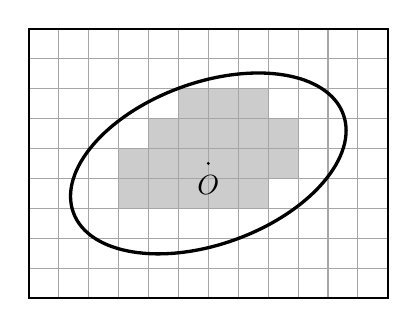
\begin{tikzpicture}[scale=0.38]
  % 填充完全在椭圆内的格子 (Ii \subset Omega)
  \foreach \x/\y in {
    3/3, 4/3, 5/3, 6/3, 7/3,
    3/4, 4/4, 5/4, 6/4, 7/4, 8/4,
    4/5, 5/5, 6/5, 7/5, 8/5,
    5/6, 6/6, 7/6
  } {
    \fill[gray!40] (\x, \y) rectangle (\x+1, \y+1);
  }
  % 网格线
  \draw[step=1, thin, gray!70] (0,0) grid (12,9);
  \draw[thick] (0,0) rectangle (12,9);
  
  % 椭圆
  \draw[very thick] (6, 4.5) ellipse [x radius=4.8, y radius=2.7, rotate=20];
  \fill (6, 4.5) circle (1.5pt) node[below=1pt] {$O$};
\end{tikzpicture}
\end{minipage}\hfill
\begin{minipage}{0.48\linewidth}
\centering
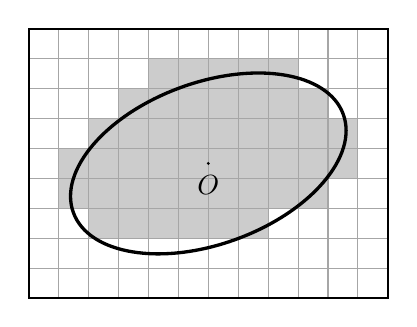
\begin{tikzpicture}[scale=0.38]
  % 填充与椭圆相交的格子 (Omega \cap Ii \neq \emptyset)
  \foreach \x/\y in {
    2/2, 3/2, 4/2, 5/2, 6/2, 7/2,
    1/3, 2/3, 3/3, 4/3, 5/3, 6/3, 7/3, 8/3, 9/3,
    1/4, 2/4, 3/4, 4/4, 5/4, 6/4, 7/4, 8/4, 9/4, 10/4,
    2/5, 3/5, 4/5, 5/5, 6/5, 7/5, 8/5, 9/5, 10/5,
    3/6, 4/6, 5/6, 6/6, 7/6, 8/6, 9/6,
    4/7, 5/7, 6/7, 7/7, 8/7
  } {
    \fill[gray!40] (\x, \y) rectangle (\x+1, \y+1);
  }
  % 网格线
  \draw[step=1, thin, gray!70] (0,0) grid (12,9);
  \draw[thick] (0,0) rectangle (12,9);
  
  % 椭圆
  \draw[very thick] (6, 4.5) ellipse [x radius=4.8, y radius=2.7, rotate=20];
  \fill (6, 4.5) circle (1.5pt) node[below=1pt] {$O$};
\end{tikzpicture}
\end{minipage}
\caption{}
\label{fig:10.2.2}
\end{figure}

\setcounter{definition}{2}
\begin{definitionp}{有面积集的等价定义}\label{def:10.2.2p}
设 $\Omega \subset \mathbb{R}^2$ 为有界集, 闭区间 $I \supset \Omega$, 对 $I$ 的分割 $T = \{I_1, I_2, \cdots, I_k\}$, 有
\[
\bigcup_{I_i\subset\Omega}I_i \subset \Omega \subset \bigcup_{\Omega\cap I_i\neq\varnothing}I_i.
\]
如果
\[
\lim_{\|T\|\to 0}\sum_{\Omega\cap I_i\neq\varnothing}v(I_i) = \lim_{\|T\|\to 0}\sum_{I_i\subset\Omega}v(I_i),
\]
则称 $\Omega$ 为有面积集, 并称 $\lim_{\|T\|\to 0}\sum_{\Omega\cap I_i\neq\varnothing}v(I_i) = \lim_{\|T\|\to 0}\sum_{I_i\subset\Omega}v(I_i)$ 为 $\Omega$ 的面积, 记为 $v(\Omega)$.
\end{definitionp}

\begin{theorem}[有面积集的几何特征二]\label{thm:10.2.5}
设 $\Omega \subset \mathbb{R}^2$ 为有界集. 则 $($图 \ref{fig:10.2.2}$)$
\[
\Omega \text{ 为有面积集} \iff \partial\Omega \text{ 为零面积集, 即 } v(\partial\Omega)=0.
\]
\end{theorem}

\begin{proof}
($\Leftarrow$) 设 $\partial\Omega$ 为零面积集, 即 $v(\partial\Omega)=0$. 又因 1 在 $\Omega$ 上连续, 故 $D_{\text{不}}^1 = \varnothing$, 当然是零面积集. 根据定理 \ref{thm:10.1.4} 知, $\partial\Omega$ 与 $D_{\text{不}}^1$ 都为零测集, 再由定理 \ref{thm:10.2.1} 推得函数 1 在 $\Omega$ 上可积, 即 $\Omega$ 为有面积集.

($\Rightarrow$) 设 $\Omega$ 为有面积集. 任取闭区间 $I \supset \Omega$, 由定理 \ref{thm:10.2.4}, $\forall\varepsilon>0$, $\exists\delta>0$, 当 $\|T\|<\delta$ 时, 有
\[
\sum_{\substack{\Omega\cap I_i\neq\varnothing \\ I_i\not\subset\Omega}}v(I_i) = \sum_{\Omega\cap I_i\neq\varnothing}v(I_i) - \sum_{I_i\subset\Omega}v(I_i) < \frac{\varepsilon}{2}.
\]
固定分割 $T=\{I_1,I_2,\cdots,I_k\}$, 显然 $\bigcup_{i=1}^{k}\partial I_i$ 为零面积集, 从而存在闭区间 $J_1,J_2,\cdots,J_s$, 使得
\[
\bigcup_{i=1}^{k}\partial I_i \subset \bigcup_{j=1}^{s}J_j, \quad \text{且} \quad \sum_{j=1}^{s}v(J_j) < \frac{\varepsilon}{2}.
\]
于是
\[
\partial\Omega \subset \left(\bigcup_{\substack{\Omega\cap I_i\neq\varnothing \\ I_i\not\subset\Omega}}I_i\right) \cup \left(\bigcup_{i=1}^{k}\partial I_i\right) \subset \left(\bigcup_{\substack{\Omega\cap I_i\neq\varnothing \\ I_i\not\subset\Omega}}I_i\right) \cup \left(\bigcup_{j=1}^{s}J_j\right),
\]
且
\[
\sum_{\substack{\Omega\cap I_i\neq\varnothing \\ I_i\not\subset\Omega}}v(I_i) + \sum_{j=1}^{s}v(J_j) < \frac{\varepsilon}{2} + \frac{\varepsilon}{2} = \varepsilon.
\]
这就证明了 $\partial\Omega$ 为零面积集. 再根据定理 \ref{thm:10.2.3}, $v(\partial\Omega)=\int_{\partial\Omega}1=0$.
\end{proof}

\begin{example}\label{ex:10.2.2}
由定理 \ref{thm:10.1.4} 中反例知, $\mathbb{Q}^2 \cap [0,1]^2$ 为 $\mathbb{R}^2$ 中的有界非零面积集. 再由 $v(\partial(\mathbb{Q}^2 \cap [0,1]^2)) = v([0,1]^2) = 1 \neq 0$ 及定理 \ref{thm:10.2.5} 推得 $\mathbb{Q}^2 \cap [0,1]^2$ 不为有面积集. 根据定义 \ref{def:10.2.2}, 1 在 $\Omega$ 上不可积.
\end{example}

\setcounter{definition}{2}
\begin{definitionpp}{有面积集的等价定义}\label{def:10.2.2pp}
设 $\Omega \subset \mathbb{R}^2$ 为有界集. 如果 $\partial\Omega$ 为零面积集, 则称 $\Omega$ 为有面积集.
\end{definitionpp}

因为有时对 $\partial\Omega$ 是否为零面积集的判断比较容易, 所以用这种方法判断 $\Omega$ 是否为有面积集也比较容易. 但是, 这定义不能给出 $\Omega$ 的面积的大小.

\begin{theorem}[有面积集上函数可积的充要条件]\label{thm:10.2.6}
设 $\Omega \subset \mathbb{R}^2$ 为有面积集, $f\colon \Omega \to \mathbb{R}$ 为有界二元函数. 则
\begin{align*}
f \text{ 在 } \Omega \text{ 上可积} &\iff D_{\text{不}}^f = \{(x, y) \in \Omega \mid f \text{ 在 } (x, y) \text{ 处不连续}\} \text{ 为零测集}, \\
&\quad\text{即 } f \text{ 在 } \Omega \text{ 上几乎处处连续}.
\end{align*}
\end{theorem}

\begin{proof}
因为 $\Omega$ 为有面积集, 根据定理 \ref{thm:10.2.5} 知, $\partial\Omega$ 与 $\partial\Omega\cap\Omega$ 都为零面积集, 当然它们也为零测集.

设闭区间 $I \supset \Omega$, 则 $\Omega = \Omega^\circ \cup (\partial \Omega \cap \Omega)$, 且
\[
I = \Omega^\circ \cup \partial\Omega \cup (I\setminus\Omega)^\circ \cup \partial I.
\]
显然, $\partial I$ 为零面积集, 自然也为零测集. 此外, 易见,
\begin{gather*}
f \text{ 在 } \boldsymbol{x} \in \Omega \text{ 不连续} \implies f_{\Omega} \text{ 在 } \boldsymbol{x} \in \Omega \text{ 不连续}; \\
f \text{ 在 } \boldsymbol{x} \in \Omega^\circ \text{ 不连续} \iff f_{\Omega} \text{ 在 } \boldsymbol{x} \in \Omega^\circ \text{ 不连续};
\end{gather*}
$f_{\Omega}$ 在 $(I\setminus\Omega)^\circ$ 上恒为 0, 故它连续.
于是
\[
\begin{cases}
D_{\text{不}}^f \subset D_{\text{不}}^{f_{\Omega}}, \\
D_{\text{不}}^{f_{\Omega}} \subset D_{\text{不}}^f \cup \partial\Omega \cup \partial I.
\end{cases}
\]
这就可推出
\begin{align*}
f \text{ 在 } \Omega \text{ 上可积} &\iff f_{\Omega} \text{ 在 } I \text{ 上可积} \iff D_{\text{不}}^{f_{\Omega}} \text{ 为零测集} \\
&\iff D_{\text{不}}^f \text{ 为零测集, 即 } f \text{ 在 } \Omega \text{ 上几乎处处连续}. \qedhere
\end{align*}
\end{proof}

注意, 0 在任何有界集 $\Omega \subset \mathbb{R}^2$ 上都可积, 不必要求 $\Omega$ 为有面积集. 而定理 \ref{thm:10.2.6} 是在 $\Omega$ 为有面积集的前提下 $f$ 可积的充要条件. 定义 \ref{def:10.2.2} 表明 1 在 $\Omega$ 上可积就是 $\Omega$ 为有面积集.

\begin{example}\label{ex:10.2.3}
设 $\Omega$ 为有限段显式表示的连续曲线围成的区域 (图 \ref{fig:10.2.3}), 根据例 \ref{ex:10.1.1} 知 $\partial\Omega$ 为零面积集, 即 $v(\partial\Omega)=0$. 再根据定理 \ref{thm:10.2.5}, $\Omega$ 为有面积集.

同理, 若 $\Omega$ 为有限段 $C^1$ 参数曲线围成的区域 (图 \ref{fig:10.2.4}), 根据例 \ref{ex:10.1.2} 知, $\partial\Omega$ 为零面积集. 再由定理 \ref{thm:10.2.5}, $\Omega$ 为有面积集.
\end{example}

\begin{figure}[htbp]
\centering
\begin{minipage}{0.48\linewidth}
\centering
\begin{tikzpicture}[scale=0.9, >=Stealth]
  % 坐标轴
  \draw[->] (-0.3, 0) -- (4.2, 0) node[below] {$x$};
  \draw[->] (0, -0.3) -- (0, 3.6) node[left] {$y$};
  \node[below left] at (0,0) {$O$};
  
  % 区域四条曲线:
  \begin{scope}
    \path[clip] (0.5, 0.9) to[bend right=10] (1.1, 0.5)
                           to[bend right=12] (3.0, 0.9)
                           to[bend left=10] (2.3, 2.3)
                           to[bend left=15] (0.5, 0.9);
    \fill[pattern=north east lines, pattern color=black!70] (0,0) rectangle (4,4);
  \end{scope}
  \draw[thick] (0.5, 0.9) to[bend right=10] (1.1, 0.5)
                          to[bend right=12] (3.0, 0.9)
                          to[bend left=10] (2.3, 2.3)
                          to[bend left=15] (0.5, 0.9);
  \node at (1.8, 1.3) {$\Omega$};
  
  % 曲线标注
  \node[left, rotate=38] at (0.7, 0.6) {\scriptsize $x=g_1(y)$};
  \node[below] at (2.0, 0.65) {\scriptsize $y=f_1(x)$};
  \node[right, rotate=-55] at (2.7, 1.7) {\scriptsize $x=g_2(y)$};
  \node[above, rotate=38] at (1.3, 1.8) {\scriptsize $y=f_2(x)$};
\end{tikzpicture}
\caption{}
\label{fig:10.2.3}
\end{minipage}\hfill
\begin{minipage}{0.48\linewidth}
\centering
\begin{tikzpicture}[scale=0.9, >=Stealth]
  % 坐标轴
  \draw[->] (-0.3, 0) -- (4.2, 0) node[below] {$x$};
  \draw[->] (0, -0.3) -- (0, 3.6) node[left] {$y$};
  \node[below left] at (0,0) {$O$};
  
  % 梅花状参数曲线
  \begin{scope}
    \path[clip] (2.0, 0.5) to[out=20, in=200] (2.8, 0.6)
                           to[out=60, in=-40] (2.6, 1.4)
                           to[out=0, in=-90] (3.3, 2.0)
                           to[out=90, in=0] (2.5, 2.6)
                           to[out=140, in=40] (1.5, 2.6)
                           to[out=180, in=90] (0.7, 2.0)
                           to[out=-90, in=180] (1.4, 1.4)
                           to[out=-140, in=120] (1.2, 0.6)
                           to[out=-20, in=160] (2.0, 0.5);
    \fill[pattern=north east lines, pattern color=black!70] (0,0) rectangle (4,4);
  \end{scope}
  \draw[thick] (2.0, 0.5) to[out=20, in=200] (2.8, 0.6)
                          to[out=60, in=-40] (2.6, 1.4)
                          to[out=0, in=-90] (3.3, 2.0)
                          to[out=90, in=0] (2.5, 2.6)
                          to[out=140, in=40] (1.5, 2.6)
                          to[out=180, in=90] (0.7, 2.0)
                          to[out=-90, in=180] (1.4, 1.4)
                          to[out=-140, in=120] (1.2, 0.6)
                          to[out=-20, in=160] (2.0, 0.5);
  \node at (2.0, 1.7) {$\Omega$};
  \node[right] at (3.3, 2.0) {\small $(x(t), y(t))$};
\end{tikzpicture}
\caption{}
\label{fig:10.2.4}
\end{minipage}
\end{figure}

上面所述的区域 $\Omega$ 是数学分析中常见的集合. 再从定理 \ref{thm:10.2.6} 立即得到
\[
f\colon\Omega\to\mathbb{R} \text{ 可积} \iff f \text{ 在 } \Omega \text{ 上几乎处处连续}.
\]

最后, 我们来讨论可积函数的一些性质.

\begin{theorem}\label{thm:10.2.7}
设 $\Omega \subset \mathbb{R}^2$ 为有界集, $f, f_1, f_2\colon \Omega \to \mathbb{R}$ 都为二元函数, $c \in \mathbb{R}$ 为常数.
\begin{enumerate}
\item 如果 $\Omega$ 为有面积集, 则 $c$ 在 $\Omega$ 上可积, 且
\[
\int_{\Omega}c = c v(\Omega).
\]
\item 如果 $f$ 在 $\Omega$ 上可积, 则 $cf$ 在 $\Omega$ 上也可积, 且
\[
\int_{\Omega}cf = c\int_{\Omega}f.
\]
\item 如果 $f_{1}$ 与 $f_{2}$ 都在 $\Omega$ 上可积, 则 $f_{1} + f_{2}$ 在 $\Omega$ 上也可积, 且
\[
\int_{\Omega}(f_{1}+f_{2}) = \int_{\Omega}f_{1} + \int_{\Omega}f_{2}.
\]
\item 如果 $f$ 在 $\Omega$ 上可积, 且 $f \geqslant 0$, 则
\[
\int_{\Omega}f \geqslant 0;
\]
特别地, 若 $f_{1}$ 与 $f_{2}$ 都在 $\Omega$ 上可积, 且 $f_{1} \geqslant f_{2}$, 则
\[
\int_{\Omega}f_{1} \geqslant \int_{\Omega}f_{2}.
\]
\item 如果 $f$ 在 $\Omega$ 上可积, 则 $|f|$ 在 $\Omega$ 上也可积, 且
\[
\left|\int_{\Omega}f\right| \leqslant \int_{\Omega}|f|.
\]
\end{enumerate}
\end{theorem}

\begin{proof}
设 $I \subset \mathbb{R}^2$ 为闭区间, 且 $I \supset \Omega$. 先证 (2), 再证 (1).

(2) $\int_{\Omega} cf = \int_{I}(cf)_{\Omega} = \int_{I} cf_{\Omega} = c\int_{I} f_{\Omega} = c\int_{\Omega} f$.

(1) 因为 $\Omega$ 为有面积集, 由 (2) 知 $c = c \cdot 1$ 在 $\Omega$ 上也可积, 且
\[
\int_{\Omega}c = \int_{\Omega}c \cdot 1 = c\int_{\Omega}1 = c v(\Omega).
\]

(3) 因为 $f_{1}$ 与 $f_{2}$ 都在 $\Omega$ 上可积, 故 $f_{1\Omega}$ 与 $f_{2\Omega}$ 都在 $I$ 上可积, 从而 $(f_{1}+f_{2})_{\Omega}=f_{1\Omega}+f_{2\Omega}$ 也在 $I$ 上可积, 即 $f_{1}+f_{2}$ 在 $\Omega$ 上可积, 且
\[
\int_{\Omega}(f_{1}+f_{2}) = \int_{I}(f_{1}+f_{2})_{\Omega} = \int_{I}(f_{1\Omega}+f_{2\Omega}) = \int_{I}f_{1\Omega} + \int_{I}f_{2\Omega} = \int_{\Omega}f_{1} + \int_{\Omega}f_{2}.
\]

(4) 因为在 $\Omega$ 上 $f \geqslant 0$, 所以 $f_{\Omega} \geqslant 0$. 根据定理 \ref{thm:10.1.1}(4), 有
\[
\int_{\Omega}f = \int_{I}f_{\Omega} \geqslant 0.
\]
从而
\[
\int_{\Omega}f_{1} - \int_{\Omega}f_{2} = \int_{\Omega}(f_{1}-f_{2}) \geqslant 0,
\]
\[
\int_{\Omega}f_{1} \geqslant \int_{\Omega}f_{2}.
\]

(5) 因为 $f$ 在 $\Omega$ 上可积, 所以 $f_{\Omega}$ 在 $I$ 上可积, 从而 $|f|_{\Omega}=|f_{\Omega}|$ 在 $I$ 上可积. 再由
\[
-|f| \leqslant f \leqslant |f|
\]
及 (4) 得到
\begin{gather*}
-\int_{\Omega}|f| \leqslant \int_{\Omega}f \leqslant \int_{\Omega}|f|, \\
\left|\int_{\Omega}f\right| \leqslant \int_{\Omega}|f|. \qedhere
\end{gather*}
\end{proof}

\begin{theorem}[积分的集合可加性]\label{thm:10.2.8}
设 $\Omega_{1}, \Omega_{2} \subset \mathbb{R}^{2}$ 都为有界集, 且 $\Omega_{1} \cap \Omega_{2}$ 为一零面积集 $(\Omega_{1} \cap \Omega_2 = \varnothing$ 为其特例$)$. 若函数 $f$ 在 $\Omega_{1}$ 与 $\Omega_{2}$ 上都可积, 则 $f$ 在 $\Omega_{1} \cup \Omega_{2}$ 上也可积, 且
\[
\int_{\Omega_{1}\cup\Omega_{2}}f = \int_{\Omega_{1}}f + \int_{\Omega_{2}}f.
\]
\end{theorem}

\begin{proof}
显然, 除了一个零面积集, 成立等式 $f_{\Omega_1 \cup \Omega_2} = f_{\Omega_1} + f_{\Omega_2}$. 设闭区间 $I \supset \Omega_1 \cup \Omega_2$, 则有
\[
\int_{\Omega_{1}}f + \int_{\Omega_{2}}f = \int_{I}f_{\Omega_{1}} + \int_{I}f_{\Omega_{2}} = \int_{I}(f_{\Omega_{1}}+f_{\Omega_{2}}) \reason{\text{例 \ref{ex:10.1.5}}} \int_{I}f_{\Omega_{1}\cup\Omega_{2}} = \int_{\Omega_{1}\cup\Omega_{2}}f. \qedhere
\]
\end{proof}

\begin{theorem}[积分中值定理]\label{thm:10.2.9}
设 $\Omega \subset \mathbb{R}^2$ 为有面积的连通紧致集, $f, g\colon \Omega \to \mathbb{R}$ 连续, 且 $g$ 在 $\Omega$ 上不变号, 则 $\exists\boldsymbol{\xi} \in \Omega$, s.t.
\[
\int_{\Omega}f g = f(\boldsymbol{\xi})\int_{\Omega}g.
\]
特别地, 取 $g=1$, 则 $\exists\boldsymbol{\xi} \in \Omega$, s.t.
\[
\int_{\Omega}f = f(\boldsymbol{\xi})v(\Omega).
\]
\end{theorem}

\begin{proof}
因为 $\Omega$ 为有面积集, 根据定理 \ref{thm:10.2.5}, $v(\partial\Omega)=0$ (即 $\partial\Omega$ 为零面积集). 由于 $f, g$ 在 $\Omega$ 上连续, 故 $fg$ 在 $\Omega$ 上也连续. 再根据定理 \ref{thm:10.2.1} 或定理 \ref{thm:10.2.6}, $g$ 与 $fg$ 都在 $\Omega$ 上可积. 又因 $\Omega$ 紧致, 故连续函数 $f$ 在 $\Omega$ 上达到最大值与最小值, 所以 $\exists\boldsymbol{p}, \boldsymbol{q} \in \Omega$, s.t.
\[
f(\boldsymbol{p}) = \max f(\Omega), \quad f(\boldsymbol{q}) = \min f(\Omega).
\]
从题设 $g$ 在 $\Omega$ 上不变号, 不妨设 $g|_{\Omega} \geqslant 0$. 于是
\[
f(\boldsymbol{q})g \leqslant fg \leqslant f(\boldsymbol{p})g.
\]
根据定理 \ref{thm:10.2.7}(4), (2), 有
\[
f(\boldsymbol{q})\int_{\Omega}g \leqslant \int_{\Omega}fg \leqslant f(\boldsymbol{p})\int_{\Omega}g.
\]
(1) 若 $\int_{\Omega}g=0$, 由 $g$ 非负连续, $g|_{\Omega}\equiv 0$, 则 $\int_{\Omega}fg=0=f(\boldsymbol{\xi})\cdot 0=f(\boldsymbol{\xi})\int_{\Omega}g$, $\forall\boldsymbol{\xi}\in\Omega$.

(2) 若 $\int_{\Omega}g\neq 0$, 由 $g\geqslant 0$ 知 $\int_{\Omega}g>0$. 于是
\[
f(\boldsymbol{q}) \leqslant \frac{\displaystyle\int_{\Omega}fg}{\displaystyle\int_{\Omega}g} \leqslant f(\boldsymbol{p}).
\]
再由 $\Omega$ 连通, 应用连续函数的介值定理, $\exists\boldsymbol{\xi}\in\Omega$, s.t.
\[
\frac{\displaystyle\int_{\Omega}fg}{\displaystyle\int_{\Omega}g} = f(\boldsymbol{\xi}),
\]
即
\[
\int_{\Omega}fg = f(\boldsymbol{\xi})\int_{\Omega}g. \qedhere
\]
\end{proof}

\begin{exblock}{练习题 10.2}
1. 设 $f$ 为连续函数, 求极限
\[
\lim_{r \to 0}\frac{1}{\pi r^2}\iint_{x^2 + y^2 \leqslant r^2} f(x, y)\,\mathrm{d}x\mathrm{d}y.
\]

2. 证明:
\[
1.96 < \iint_{|x|+|y|\leqslant 10}\frac{\mathrm{d}x\mathrm{d}y}{100 + \cos^2 x + \cos^2 y} < 2.
\]
\end{exblock}

\section{化二重积分为累次积分}\label{sec:10.3}

在第 \ref{sec:10.1} 节中，我们建立了二重积分的定义，并且证明了二重积分具有类似于定积分的许多性质。
但是，直接由定义计算二重积分，即使对比较简单的函数与区域来说，也是很困难的。
为了求出二重积分的值，必须寻找更方便的计算方法。
在微积分学中，计算重积分的基本方法是：把重积分化为一连串的一元函数的定积分（通常称为累次积分或多次积分）来计算。
本节我们来讨论如何把二重积分化为两次定积分来计算。

首先，我们讨论在闭矩形区间上的情形。

\begin{theorem}\label{thm:10.3.1}
设 $I = [a, b] \times [c, d]$ 为 $\mathbb{R}^2$ 中的闭区间，$f\colon I \to \mathbb{R}$ 可积，则单变量函数
\[
I_1(x) = \overline{\int_c^d} f(x, y)\,\mathrm{d}y, \quad I_2(x) = \underline{\int_c^d} f(x, y)\,\mathrm{d}y
\]
在 $[a, b]$ 上都可积，且
\[
\int_a^b \overline{\int_c^d} f(x, y)\,\mathrm{d}y\,\mathrm{d}x = \int_a^b \underline{\int_c^d} f(x, y)\,\mathrm{d}y\,\mathrm{d}x = \iint_I f(x, y)\,\mathrm{d}x\mathrm{d}y.
\]
\end{theorem}

\begin{proof}
设 $T_1 = \{a = x_0 < x_1 < \cdots < x_m = b\}$ 与 $T_2 = \{c = y_0 < y_1 < \cdots < y_k = d\}$ 分别为 $[a, b]$ 与 $[c, d]$ 的任意分割。
它们构成了闭区间 $I$ 的一个网格分割 $T = T_1 \times T_2$。
记
\[
I_{ij} = [x_{i-1}, x_i] \times [y_{j-1}, y_j], \quad v(I_{ij}) = \Delta x_i \Delta y_j = (x_i - x_{i-1})(y_j - y_{j-1}),
\]
\[
m_{ij} = \inf_{(x, y) \in I_{ij}} f(x, y), \quad M_{ij} = \sup_{(x, y) \in I_{ij}} f(x, y).
\]
对于固定的 $x \in [x_{i-1}, x_i]$，记
\[
m_j(x) = \inf_{y \in [y_{j-1}, y_j]} f(x, y), \quad M_j(x) = \sup_{y \in [y_{j-1}, y_j]} f(x, y).
\]
显然对任意 $y \in [y_{j-1}, y_j]$，恒有 $m_{ij} \leqslant m_j(x) \leqslant f(x, y) \leqslant M_j(x) \leqslant M_{ij}$。
从而根据上、下积分的定义与性质，有
\[
\sum_{j=1}^k m_{ij} \Delta y_j \leqslant \sum_{j=1}^k m_j(x) \Delta y_j \leqslant \underline{\int_c^d} f(x, y)\,\mathrm{d}y \leqslant \overline{\int_c^d} f(x, y)\,\mathrm{d}y \leqslant \sum_{j=1}^k M_j(x) \Delta y_j \leqslant \sum_{j=1}^k M_{ij} \Delta y_j.
\]
上式对任意 $x \in [x_{i-1}, x_i]$ 均成立。
故在区间 $[x_{i-1}, x_i]$ 上分别取 $I_1(x) = \overline{\int_c^d} f(x, y)\,\mathrm{d}y$ 与 $I_2(x) = \underline{\int_c^d} f(x, y)\,\mathrm{d}y$ 的下确界与上确界，即知
\[
\sum_{j=1}^k m_{ij} \Delta y_j \leqslant \inf_{x \in [x_{i-1}, x_i]} I_2(x) \leqslant \sup_{x \in [x_{i-1}, x_i]} I_1(x) \leqslant \sum_{j=1}^k M_{ij} \Delta y_j.
\]
两边同乘以 $\Delta x_i$，并对 $i = 1, 2, \dots, m$ 求和，得
\[
s(T, f) = \sum_{i=1}^m \sum_{j=1}^k m_{ij} \Delta x_i \Delta y_j \leqslant s(T_1, I_2) \leqslant s(T_1, I_1) \leqslant S(T_1, I_1) \leqslant S(T, f).
\]
同理亦有
\[
s(T, f) \leqslant s(T_1, I_2) \leqslant S(T_1, I_2) \leqslant S(T_1, I_1) \leqslant S(T, f).
\]
因 $f$ 在 $I$ 上可积，故当 $\|T\| \to 0$ 时，Darboux 和极限存在且
\[
\lim_{\|T\| \to 0} s(T, f) = \lim_{\|T\| \to 0} S(T, f) = \iint_I f(x, y)\,\mathrm{d}x\mathrm{d}y.
\]
注意 $\|T_1\| \leqslant \|T\|$，由夹逼准则立即推得：$I_1(x)$ 与 $I_2(x)$ 在 $[a, b]$ 上均满足 Riemann 可积准则，从而在 $[a, b]$ 上可积，且极限值恰为 $\iint_I f(x, y)\,\mathrm{d}x\mathrm{d}y$。
\end{proof}

由定理 \ref{thm:10.3.1} 立即得到下面两个重要推论：

\begin{theorem}[闭区间上化二重积分为累次积分]\label{thm:10.3.2}
设 $f$ 在闭区间 $I = [a, b] \times [c, d]$ 上可积。如果对每个固定的 $x \in [a, b]$，函数 $f(x, \cdot)$ 在 $[c, d]$ 上都可积，则
\[
\iint_I f(x, y)\,\mathrm{d}x\mathrm{d}y = \int_a^b \mathrm{d}x \int_c^d f(x, y)\,\mathrm{d}y = \int_a^b \left( \int_c^d f(x, y)\,\mathrm{d}y \right) \mathrm{d}x.
\]
\end{theorem}

\begin{proof}
因 $f(x, \cdot)$ 在 $[c, d]$ 上可积，故对每个 $x \in [a, b]$，其上积分与下积分相等：
\[
\overline{\int_c^d} f(x, y)\,\mathrm{d}y = \underline{\int_c^d} f(x, y)\,\mathrm{d}y = \int_c^d f(x, y)\,\mathrm{d}y.
\]
代入定理 \ref{thm:10.3.1} 即得所证。
\end{proof}

同理，若先对 $x$ 积分再对 $y$ 积分，亦有完全对称的结论：

\begin{theorem}[闭区间上化二重积分为累次积分]\label{thm:10.3.3}
设 $f$ 在 $I = [a, b] \times [c, d]$ 上可积，且对每个 $x \in [a, b]$，$f(x, \cdot)$ 在 $[c, d]$ 上可积；又对每个 $y \in [c, d]$，$f(\cdot, y)$ 在 $[a, b]$ 上可积，则
\[
\iint_I f(x, y)\,\mathrm{d}x\mathrm{d}y = \int_a^b \mathrm{d}x \int_c^d f(x, y)\,\mathrm{d}y = \int_c^d \mathrm{d}y \int_a^b f(x, y)\,\mathrm{d}x.
\]
特别地，当 $f$ 在 $I$ 上连续时，上述可积性条件自然满足，累次积分顺序可以任意交换。
\end{theorem}

现在，我们把闭矩形区间上的结论推广到一般的有界有面积集 $\Omega \subset \mathbb{R}^2$ 上。

\begin{figure}[htbp]
\centering
\begin{tikzpicture}[>=Stealth, scale=1.0]
  \draw[->] (-0.3,0) -- (5.2,0) node[below] {$x$};
  \draw[->] (0,-0.3) -- (0,4.2) node[left] {$y$};
  \node[below left] at (0,0) {$O$};

  \coordinate (A) at (1.0,0);
  \coordinate (X) at (2.2,0);
  \coordinate (B) at (4.4,0);
  \coordinate (C) at (0,0.8);
  \coordinate (Y) at (0,2.3);
  \coordinate (D) at (0,3.6);

  \node[below] at (A) {$a$};
  \node[below] at (X) {$x$};
  \node[below] at (B) {$b$};
  \node[left] at (C) {$c$};
  \node[left] at (Y) {$y$};
  \node[left] at (D) {$d$};

  \draw[dashed] (1.0,0) -- (1.0,3.8);
  \draw[dashed] (4.4,0) -- (4.4,3.8);
  \draw[dashed] (0,0.8) -- (4.8,0.8);
  \draw[dashed] (0,3.6) -- (4.8,3.6);

  \draw[dashed] (2.2,0) -- (2.2,1.35);
  \draw[dashed] (2.2,2.95) -- (2.2,3.8);
  \draw[dashed] (0,2.3) -- (1.35,2.3);
  \draw[dashed] (3.65,2.3) -- (4.8,2.3);

  \draw[thick, fill=black!15] 
    (1.3, 2.0) .. controls (1.5, 2.9) and (2.5, 3.1) .. (3.2, 2.8)
    .. controls (3.6, 2.6) and (3.8, 2.3) .. (4.2, 2.7)
    -- (4.2, 1.4)
    .. controls (3.8, 1.8) and (3.6, 1.5) .. (3.2, 1.3)
    .. controls (2.5, 1.0) and (1.5, 1.2) .. (1.3, 2.0) -- cycle;

  \draw[very thick] (2.2, 1.15) -- (2.2, 2.97);
  \node[right] at (2.2, 1.7) {$\Omega_x$};

  \draw[very thick] (1.33, 2.3) -- (3.68, 2.3);
  \node[above] at (1.8, 2.3) {$\Omega^y$};

  \node at (2.9, 2.0) {$\Omega$};

  \draw[decorate, decoration={brace, mirror, amplitude=5pt}] (1.0, -0.3) -- (4.4, -0.3) node[midway, below=5pt] {$I$};
  \draw[decorate, decoration={brace, amplitude=5pt}] (-0.3, 0.8) -- (-0.3, 3.6) node[midway, left=5pt] {$J$};
\end{tikzpicture}
\caption{}\label{fig:10.3.1}
\end{figure}

\begin{theorem}[有界集上化二重积分为累次积分]\label{thm:10.3.4}
设 $\Omega \subset \mathbb{R}^2$ 为有面积集，$f\colon \Omega \to \mathbb{R}$ 有界且连续。记 $\Omega$ 在 $x$ 轴上的垂直投影（图 \ref{fig:10.3.1}）为
\[
I = \{x \in \mathbb{R} \mid \exists y, \text{ s.t. } (x, y) \in \Omega\}.
\]
如果对每个 $x \in I$，截线集 $\Omega_x = \{y \in \mathbb{R} \mid (x, y) \in \Omega\}$ 为一个或有限个区间的并（可以退缩为单点），则
\[
\iint_\Omega f = \int_I \mathrm{d}x \int_{\Omega_x} f(x, y)\,\mathrm{d}y.
\]
同样，记 $\Omega$ 在 $y$ 轴上的垂直投影（图 \ref{fig:10.3.1}）为
\[
J = \{y \in \mathbb{R} \mid \exists x, \text{ s.t. } (x, y) \in \Omega\}.
\]
如果对每个 $y \in J$，截线集 $\Omega^y = \{x \in \mathbb{R} \mid (x, y) \in \Omega\}$ 为一个或有限个区间的并（可以退缩为单点），则
\[
\iint_\Omega f = \int_J \mathrm{d}y \int_{\Omega^y} f(x, y)\,\mathrm{d}x.
\]
\end{theorem}

\begin{proof}
作闭区间 $[a, b] \times [c, d] \supset \Omega$（图 \ref{fig:10.3.1}）。
因为 $f$ 在 $\Omega$ 上有界连续，并且 $\Omega \subset \mathbb{R}^2$ 为有面积集，根据定理 \ref{thm:10.2.6}，$f$ 在 $\Omega$ 上可积。
再由定义 \ref{def:10.2.1}，零延拓函数 $f_\Omega$ 在 $[a, b] \times [c, d]$ 上可积，且
\[
\iint_\Omega f = \iint_{[a, b] \times [c, d]} f_\Omega.
\]
当 $x \in I$ 时，函数 $f(x, \cdot)$ 在区间 $\Omega_x$ 上有界且连续，所以 $f(x, \cdot)$ 在 $\Omega_x$ 上可积。
又因在 $[c, d] \setminus \Omega_x$ 上 $f_\Omega(x, y) = 0$，故 $f_\Omega(x, \cdot)$ 在 $[c, d]$ 上可积，且
\[
\int_c^d f_\Omega(x, y)\,\mathrm{d}y = \int_{\Omega_x} f(x, y)\,\mathrm{d}y.
\]
当 $x \in [a, b] \setminus I$ 时，对一切 $y \in [c, d]$ 均有 $f_\Omega(x, y) = 0$，从而
\[
\int_c^d f_\Omega(x, y)\,\mathrm{d}y = 0.
\]
根据定理 \ref{thm:10.3.2}，有
\begin{align*}
\iint_\Omega f &= \iint_{[a, b] \times [c, d]} f_\Omega = \int_a^b \mathrm{d}x \int_c^d f_\Omega(x, y)\,\mathrm{d}y \\
&= \int_I \mathrm{d}x \int_c^d f_\Omega(x, y)\,\mathrm{d}y = \int_I \mathrm{d}x \int_{\Omega_x} f(x, y)\,\mathrm{d}y.
\end{align*}
对称地可证第二式。
\end{proof}

考虑应用中最常见的两类特殊区域（通常称为 $X$-型区域与 $Y$-型区域）：

\begin{figure}[htbp]
\centering
\begin{minipage}[b]{0.48\linewidth}
\centering
\begin{tikzpicture}[>=Stealth, scale=0.95]
  \draw[->] (-0.3,0) -- (4.2,0) node[below] {$x$};
  \draw[->] (0,-0.3) -- (0,3.8) node[left] {$y$};
  \node[below left] at (0,0) {$O$};

  \coordinate (A) at (0.9,0);
  \coordinate (X) at (1.9,0);
  \coordinate (B) at (3.5,0);
  \node[below] at (A) {$a$};
  \node[below] at (X) {$x$};
  \node[below] at (B) {$b$};

  \draw[dashed] (0, 0.8) node[left] {$c$} -- (3.8, 0.8);
  \draw[dashed] (0, 3.2) node[left] {$d$} -- (3.8, 3.2);

  \draw[dashed] (0.9, 0) -- (0.9, 1.0);
  \draw[dashed] (3.5, 0) -- (3.5, 1.1);

  \draw[thick, fill=black!15]
    (0.9, 1.0) .. controls (1.8, 1.6) and (2.6, 0.8) .. (3.5, 1.1)
    -- (3.5, 2.9)
    .. controls (2.6, 3.2) and (1.8, 2.6) .. (0.9, 2.7)
    -- cycle;

  \draw[dashed] (1.9,0) -- (1.9, 1.25);
  \draw[very thick] (1.9, 1.25) -- (1.9, 2.85);
  \node[right] at (1.9, 2.1) {$\Omega_x$};

  \node[below] at (3.0, 1.0) {$y=y_1(x)$};
  \node[above] at (3.0, 2.9) {$y=y_2(x)$};
  \node at (3.1, 2.0) {$\Omega$};
\end{tikzpicture}
\caption{}\label{fig:10.3.2}
\end{minipage}
\hfill
\begin{minipage}[b]{0.48\linewidth}
\centering
\begin{tikzpicture}[>=Stealth, scale=0.95]
  \draw[->] (-0.3,0) -- (4.2,0) node[below] {$x$};
  \draw[->] (0,-0.3) -- (0,3.8) node[left] {$y$};
  \node[below left] at (0,0) {$O$};

  \draw[dashed] (0, 0.9) node[left] {$c$} -- (3.8, 0.9);
  \draw[dashed] (0, 3.2) node[left] {$d$} -- (3.8, 3.2);

  \draw[dashed] (1.5, 0) -- (1.5, 3.5);
  \draw[dashed] (3.5, 0) -- (3.5, 3.5);

  \draw[thick, fill=black!15]
    (1.7, 0.9) .. controls (1.5, 1.8) and (2.2, 2.4) .. (1.8, 3.2)
    -- (3.4, 3.2)
    .. controls (3.8, 2.4) and (3.1, 1.8) .. (3.3, 0.9)
    -- cycle;

  \draw[dashed] (0, 2.1) node[left] {$y$} -- (1.85, 2.1);
  \draw[very thick] (1.85, 2.1) -- (3.3, 2.1);
  \node[above] at (2.6, 2.1) {$\Omega^y$};

  \node[left] at (1.7, 1.4) {$x=x_1(y)$};
  \node[right] at (3.3, 1.4) {$x=x_2(y)$};
  \node at (2.7, 1.3) {$\Omega$};
\end{tikzpicture}
\caption{}\label{fig:10.3.3}
\end{minipage}
\end{figure}

\begin{theorem}[有界集上化二重积分为累次积分]\label{thm:10.3.5}
设
\[
\Omega = \{(x, y) \in \mathbb{R}^2 \mid y_1(x) \leqslant y \leqslant y_2(x), a \leqslant x \leqslant b\},
\]
其中函数 $y_1$ 与 $y_2$ 在 $[a, b]$ 上连续（图 \ref{fig:10.3.2}），函数 $f$ 在 $\Omega$ 上可积。
如果对每个 $x \in [a, b]$，单变量积分 $\int_{y_1(x)}^{y_2(x)} f(x, y)\,\mathrm{d}y$ 存在，则
\[
\iint_\Omega f = \int_a^b \mathrm{d}x \int_{y_1(x)}^{y_2(x)} f(x, y)\,\mathrm{d}y.
\]
\end{theorem}

\begin{proof}
取闭区间 $[a, b] \times [c, d] \supset \Omega$。
对于固定的 $x \in [a, b]$，因为 $f(x, \cdot)$ 在 $[y_1(x), y_2(x)]$ 上可积，且在 $[c, y_1(x))$ 与 $(y_2(x), d]$ 上零延拓值恒为 $0$，故 $f_\Omega(x, \cdot)$ 在 $[c, d]$ 上可积，且
\begin{align*}
\int_c^d f_\Omega(x, y)\,\mathrm{d}y &= \int_c^{y_1(x)} f_\Omega(x, y)\,\mathrm{d}y + \int_{y_1(x)}^{y_2(x)} f_\Omega(x, y)\,\mathrm{d}y + \int_{y_2(x)}^d f_\Omega(x, y)\,\mathrm{d}y \\
&= 0 + \int_{y_1(x)}^{y_2(x)} f(x, y)\,\mathrm{d}y + 0 = \int_{y_1(x)}^{y_2(x)} f(x, y)\,\mathrm{d}y.
\end{align*}
根据定理 \ref{thm:10.3.2}，
\[
\iint_\Omega f = \int_a^b \mathrm{d}x \int_c^d f_\Omega(x, y)\,\mathrm{d}y = \int_a^b \mathrm{d}x \int_{y_1(x)}^{y_2(x)} f(x, y)\,\mathrm{d}y. \qedhere
\]
\end{proof}

对称地，对于 $Y$-型区域（图 \ref{fig:10.3.3}），有：

\begin{theorem}[有界集上化二重积分为累次积分]\label{thm:10.3.6}
设
\[
\Omega = \{(x, y) \in \mathbb{R}^2 \mid x_1(y) \leqslant x \leqslant x_2(y), c \leqslant y \leqslant d\},
\]
其中函数 $x_1$ 与 $x_2$ 在 $[c, d]$ 上连续（图 \ref{fig:10.3.3}），函数 $f$ 在 $\Omega$ 上可积。
如果对每个 $y \in [c, d]$，单变量积分 $\int_{x_1(y)}^{x_2(y)} f(x, y)\,\mathrm{d}x$ 存在，则
\[
\iint_\Omega f = \int_c^d \mathrm{d}y \int_{x_1(y)}^{x_2(y)} f(x, y)\,\mathrm{d}x.
\]
\end{theorem}

\begin{proof}
类似定理 \ref{thm:10.3.5} 的证明。
\end{proof}

下面我们通过一系列典型例题，详细介绍化二重积分为累次积分的具体计算方法、技巧与几何应用。

\begin{example}\label{ex:10.3.1}
计算二重积分
\[
\iint_{\substack{0 \leqslant x \leqslant 1 \\ 0 \leqslant y \leqslant 1}} x \mathrm{e}^{xy}\,\mathrm{d}x\mathrm{d}y.
\]
\end{example}

\begin{solution}
积分区域为闭矩形区间 $I = [0, 1] \times [0, 1]$，被积函数连续。
若先对 $x$ 积分，需要用分部积分法；而若先对 $y$ 积分，计算则极为简便：
\begin{align*}
\iint_I x \mathrm{e}^{xy}\,\mathrm{d}x\mathrm{d}y &= \int_0^1 \mathrm{d}x \int_0^1 x \mathrm{e}^{xy}\,\mathrm{d}y = \int_0^1 \left[ \mathrm{e}^{xy} \Big|_{y=0}^{y=1} \right] \mathrm{d}x \\
&= \int_0^1 (\mathrm{e}^x - 1)\,\mathrm{d}x = (\mathrm{e}^x - x)\Big|_0^1 = \mathrm{e} - 2. \qedhere
\end{align*}
\end{solution}

\begin{example}\label{ex:10.3.2}
计算二重积分
\[
\iint_{[0, \pi] \times [0, 1]} y \sin(xy)\,\mathrm{d}x\mathrm{d}y.
\]
\end{example}

\begin{solution}
先对 $x$ 积分再对 $y$ 积分：
\begin{align*}
\iint_{[0, \pi] \times [0, 1]} y \sin(xy)\,\mathrm{d}x\mathrm{d}y &= \int_0^1 \mathrm{d}y \int_0^\pi y \sin(xy)\,\mathrm{d}x = \int_0^1 \left[ -\cos(xy) \Big|_{x=0}^{x=\pi} \right] \mathrm{d}y \\
&= \int_0^1 (1 - \cos(\pi y))\,\mathrm{d}y = \left( y - \frac{\sin(\pi y)}{\pi} \right) \Bigg|_0^1 = 1. \qedhere
\end{align*}
\end{solution}

\begin{example}\label{ex:10.3.3}
计算
\[
\iint_{\substack{0 \leqslant x \leqslant 1 \\ 0 \leqslant y \leqslant 1}} x \mathrm{e}^{x^2+y^2}\,\mathrm{d}x\mathrm{d}y.
\]
\end{example}

\begin{solution}
由于被积函数可以分离变量 $x \mathrm{e}^{x^2+y^2} = (x \mathrm{e}^{x^2})(\mathrm{e}^{y^2})$，且积分区域为矩形，故累次积分可拆为两个独立的单变量定积分之积：
\[
\iint_{\substack{0 \leqslant x \leqslant 1 \\ 0 \leqslant y \leqslant 1}} x \mathrm{e}^{x^2+y^2}\,\mathrm{d}x\mathrm{d}y = \left( \int_0^1 x \mathrm{e}^{x^2}\,\mathrm{d}x \right) \left( \int_0^1 \mathrm{e}^{y^2}\,\mathrm{d}y \right) = \frac{1}{2}(\mathrm{e} - 1) \int_0^1 \mathrm{e}^{y^2}\,\mathrm{d}y.
\]
注意 $\int_0^1 \mathrm{e}^{y^2}\,\mathrm{d}y$ 的原函数不能用初等函数表示，但作为定积分其值是一个确定的常数。
\end{solution}

\begin{example}\label{ex:10.3.4}
计算二重积分
\[
\iint_\Omega x y^3 \mathrm{e}^{x^2+y^2}\,\mathrm{d}x\mathrm{d}y,
\]
其中 $\Omega = [0, 1] \times [0, 1]$。
\end{example}

\begin{solution}
利用乘积可分离性，有
\begin{align*}
\iint_\Omega x y^3 \mathrm{e}^{x^2+y^2}\,\mathrm{d}x\mathrm{d}y &= \left( \int_0^1 x \mathrm{e}^{x^2}\,\mathrm{d}x \right) \left( \int_0^1 y^3 \mathrm{e}^{y^2}\,\mathrm{d}y \right) \\
&= \frac{1}{2}(\mathrm{e} - 1) \cdot \frac{1}{2} \int_0^1 t \mathrm{e}^t\,\mathrm{d}t \quad (\text{令 } t = y^2) \\
&= \frac{1}{4}(\mathrm{e} - 1) \left[ t \mathrm{e}^t \Big|_0^1 - \int_0^1 \mathrm{e}^t\,\mathrm{d}t \right] \\
&= \frac{1}{4}(\mathrm{e} - 1) (\mathrm{e} - (\mathrm{e} - 1)) = \frac{1}{4}(\mathrm{e} - 1). \qedhere
\end{align*}
\end{solution}

\begin{example}\label{ex:10.3.5}
计算二重积分
\[
\iint_{\substack{0 \leqslant x \leqslant 2 \\ 0 \leqslant y \leqslant 2}} [x + y]\,\mathrm{d}x\mathrm{d}y,
\]
其中 $[u]$ 表示不超过 $u$ 的最大整数。
\end{example}

\begin{figure}[htbp]
\centering
\begin{minipage}[b]{0.48\linewidth}
\centering
\begin{tikzpicture}[>=Stealth, scale=1.3]
  \draw[->] (-0.2,0) -- (2.6,0) node[below] {$x$};
  \draw[->] (0,-0.2) -- (0,2.6) node[left] {$y$};
  \node[below left] at (0,0) {$O$};

  \draw[thick] (0,0) rectangle (2,2);
  \node[left] at (0,1) {$1$};
  \node[left] at (0,2) {$2$};
  \node[below] at (1,0) {$1$};
  \node[below] at (2,0) {$2$};

  \draw[thick] (0,1) -- (1,0);
  \draw[thick] (0,2) -- (2,0);
  \draw[thick] (1,2) -- (2,1);

  \draw[dashed] (1,0) -- (1,2);

  \node[above right, font=\footnotesize] at (0.3, 0.6) {$y=1-x$};
  \node[above right, font=\footnotesize] at (0.8, 1.1) {$y=2-x$};
  \node[above right, font=\footnotesize] at (1.3, 1.6) {$y=3-x$};
  \draw[thick] (1.7, 2.3) -- (2.3, 1.7) node[above right, font=\footnotesize] {$y=4-x$};
  \fill (2,2) circle (1.2pt) node[above left, font=\footnotesize] {$(2,2)$};
\end{tikzpicture}
\caption{}\label{fig:10.3.4}
\end{minipage}
\hfill
\begin{minipage}[b]{0.48\linewidth}
\centering
\begin{tikzpicture}[>=Stealth, scale=1.3]
  \draw[->] (-0.2,0) -- (2.6,0) node[below] {$x$};
  \draw[->] (0,-0.2) -- (0,2.6) node[left] {$y$};
  \node[below left] at (0,0) {$O$};

  \node[left] at (0,1) {$1$};
  \node[left] at (0,2) {$2$};
  \node[below] at (1,0) {$1$};
  \node[below] at (2,0) {$2$};

  \draw[thick] (0,0) rectangle (2,2);
  \draw[thick] (0,1) -- (1,0);
  \draw[thick] (0,2) -- (2,0);
  \draw[thick] (1,2) -- (2,1);

  \fill[black!20] (0,0) -- (1,0) -- (0,1) -- cycle;
  \node[font=\footnotesize] at (0.35, 0.35) {$\Omega_1$};
  \node[font=\footnotesize] at (0.2, 0.65) {$f=0$};

  \node[font=\footnotesize] at (0.9, 0.25) {$\Omega_2$};
  \node[font=\footnotesize] at (0.45, 0.95) {$f=1$};
  \node[rotate=-45, font=\tiny] at (0.8, 0.7) {$x+y=1$};

  \fill[pattern=horizontal lines, pattern color=black!70] (0,2) -- (2,0) -- (2,1) -- (1,2) -- cycle;
  \node[font=\footnotesize] at (1.6, 0.5) {$\Omega_3$};
  \node[font=\footnotesize] at (0.75, 1.75) {$f=2$};
  \node[rotate=-45, font=\tiny] at (1.2, 1.2) {$x+y=2$};

  \fill[pattern=north east lines, pattern color=black!80] (1,2) -- (2,1) -- (2,2) -- cycle;
  \node[font=\footnotesize] at (1.8, 1.7) {$\Omega_4$};
  \node[font=\footnotesize] at (1.4, 1.85) {$f=3$};
  \node[rotate=-45, font=\tiny] at (1.65, 1.65) {$x+y=3$};

  \draw[thick] (1.7, 2.3) -- (2.3, 1.7);
  \fill (2,2) circle (1.2pt) node[above left, font=\footnotesize] {$(2,2)$};
  \node[above right, font=\footnotesize] at (2.05, 1.95) {$x+y=4$};
\end{tikzpicture}
\caption{}\label{fig:10.3.5}
\end{minipage}
\end{figure}

\begin{solution}
本题给出两种解法。

\textbf{解法 1}：从图 \ref{fig:10.3.4} 可知，当 $0 \leqslant x \leqslant 1$ 时，内层积分中 $y$ 从 $0$ 到 $2$ 分为三段：$[0, 1-x]$（此时 $0 \leqslant x+y < 1$，$f=0$）、$[1-x, 2-x]$（此时 $1 \leqslant x+y < 2$，$f=1$）和 $[2-x, 2]$（此时 $2 \leqslant x+y \leqslant 3$，$f=2$）；
当 $1 \leqslant x \leqslant 2$ 时，内层积分中 $y$ 从 $0$ 到 $2$ 分为三段：$[0, 2-x]$（$f=1$）、$[2-x, 3-x]$（$f=2$）和 $[3-x, 2]$（$f=3$）。
于是
\begin{align*}
\iint_{\substack{0 \leqslant x \leqslant 2 \\ 0 \leqslant y \leqslant 2}} [x+y]\,\mathrm{d}x\mathrm{d}y &= \int_0^2 \mathrm{d}x \int_0^2 [x+y]\,\mathrm{d}y \\
&= \int_0^1 \mathrm{d}x \int_0^2 [x+y]\,\mathrm{d}y + \int_1^2 \mathrm{d}x \int_0^2 [x+y]\,\mathrm{d}y \\
&= \int_0^1 \left[ \int_0^{1-x} 0\,\mathrm{d}y + \int_{1-x}^{2-x} 1\,\mathrm{d}y + \int_{2-x}^2 2\,\mathrm{d}y \right] \mathrm{d}x \\
&\quad + \int_1^2 \left[ \int_0^{2-x} 1\,\mathrm{d}y + \int_{2-x}^{3-x} 2\,\mathrm{d}y + \int_{3-x}^2 3\,\mathrm{d}y \right] \mathrm{d}x \\
&= \int_0^1 [(2-x) - (1-x) + 2(2 - (2-x))]\,\mathrm{d}x \\
&\quad + \int_1^2 \{(2-x) + 2[(3-x)-(2-x)] + 3[2-(3-x)]\}\,\mathrm{d}x \\
&= \int_0^1 (1 + 2x)\,\mathrm{d}x + \int_1^2 (1 + 2x)\,\mathrm{d}x = \int_0^2 (1 + 2x)\,\mathrm{d}x = (x + x^2)\Big|_0^2 = 6.
\end{align*}

\textbf{解法 2}：从图 \ref{fig:10.3.5} 还可知，$\Omega = [0, 2]^2$ 上的二重积分等于 $\Omega_1, \Omega_2, \Omega_3, \Omega_4$ 上二重积分之和。
由几何面积易知：
\[
v(\Omega_1) = \frac{1}{2} \cdot 1 \cdot 1 = \frac{1}{2}, \quad v(\Omega_2) = \frac{1}{2} \cdot 2^2 - \frac{1}{2} = \frac{3}{2},
\]
\[
v(\Omega_4) = \frac{1}{2} \cdot 1 \cdot 1 = \frac{1}{2}, \quad v(\Omega_3) = 4 - v(\Omega_1) - v(\Omega_2) - v(\Omega_4) = 4 - \frac{1}{2} - \frac{3}{2} - \frac{1}{2} = \frac{3}{2}.
\]
而在各个子区域上，$f(x, y) = [x+y]$ 恰好为常数 $0, 1, 2, 3$（不计边界零面积集）。从而
\begin{align*}
\iint_\Omega [x+y]\,\mathrm{d}x\mathrm{d}y &= 0 \cdot v(\Omega_1) + 1 \cdot v(\Omega_2) + 2 \cdot v(\Omega_3) + 3 \cdot v(\Omega_4) \\
&= 0 \cdot \frac{1}{2} + 1 \cdot \frac{3}{2} + 2 \cdot \frac{3}{2} + 3 \cdot \frac{1}{2} = \frac{3}{2} + 3 + \frac{3}{2} = 6. \qedhere
\end{align*}
\end{solution}

\begin{example}\label{ex:10.3.6}
计算二重积分
\[
\iint_\Omega x^2 y^2\,\mathrm{d}x\mathrm{d}y,
\]
其中 $\Omega$ 为由 $y = \frac{b}{a}x$, $y = 0$, $x = a$ 三条直线围成的三角形（图 \ref{fig:10.3.6}，$a > 0, b > 0$）。
\end{example}

\begin{figure}[htbp]
\centering
\begin{tikzpicture}[>=Stealth, scale=1.1]
  \draw[->] (-0.3,0) -- (4.2,0) node[below] {$x$};
  \draw[->] (0,-0.3) -- (0,3.5) node[left] {$y$};
  \node[below left] at (0,0) {$O$};

  \coordinate (A) at (3.0,0);
  \coordinate (B) at (3.0,2.4);
  \coordinate (Y) at (0,1.5);
  \coordinate (X) at (1.875,0);

  \draw[thick, fill=black!20] (0,0) -- (3.0,0) -- (3.0,2.4) -- cycle;
  \draw[very thick] (0,0) -- (3.0,2.4) node[midway, above left] {$y=\frac{b}{a}x$};
  \draw[thick] (3.0,0) -- (3.0,2.4);

  \node[below] at (A) {$a$};
  \node[left] at (0,2.4) {$b$};
  \draw[dashed] (0,2.4) -- (3.0,2.4) node[above right] {$(a,b)$};

  \draw[dashed] (X) node[below] {$x$} -- (1.875,1.5);
  \draw[very thick] (1.875,0) -- (1.875,1.5);
  \node[right] at (1.875,0.75) {$\Omega_x$};

  \draw[dashed] (Y) node[left] {$y$} -- (1.875,1.5);
  \draw[very thick] (1.875,1.5) -- (3.0,1.5);
  \node[above] at (2.4,1.5) {$\Omega^y$};

  \node at (1.0, 0.4) {$\Omega$};
\end{tikzpicture}
\caption{}\label{fig:10.3.6}
\end{figure}

\begin{solution}
本题给出两种次序的解法。

\textbf{解法 1}（看成 $X$-型区域，先对 $y$ 积分）：
\[
\Omega = \left\{ (x, y) \in \mathbb{R}^2 \;\middle|\; 0 \leqslant y \leqslant \frac{b}{a}x, \; 0 \leqslant x \leqslant a \right\}.
\]
\begin{align*}
\iint_\Omega x^2 y^2\,\mathrm{d}x\mathrm{d}y &= \int_0^a \mathrm{d}x \int_0^{\frac{b}{a}x} x^2 y^2\,\mathrm{d}y = \int_0^a x^2 \left[ \frac{y^3}{3} \Bigg|_0^{\frac{b}{a}x} \right] \mathrm{d}x \\
&= \frac{1}{3} \left( \frac{b}{a} \right)^3 \int_0^a x^5\,\mathrm{d}x = \frac{b^3}{18 a^3} x^6 \Big|_0^a = \frac{1}{18} a^3 b^3.
\end{align*}

\textbf{解法 2}（看成 $Y$-型区域，先对 $x$ 积分）：
\[
\Omega = \left\{ (x, y) \in \mathbb{R}^2 \;\middle|\; \frac{a}{b}y \leqslant x \leqslant a, \; 0 \leqslant y \leqslant b \right\}.
\]
\begin{align*}
\iint_\Omega x^2 y^2\,\mathrm{d}x\mathrm{d}y &= \int_0^b \mathrm{d}y \int_{\frac{a}{b}y}^a x^2 y^2\,\mathrm{d}x = \int_0^b y^2 \left[ \frac{x^3}{3} \Bigg|_{\frac{a}{b}y}^a \right] \mathrm{d}y \\
&= \frac{1}{3} \int_0^b y^2 \left( a^3 - \frac{a^3}{b^3} y^3 \right) \mathrm{d}y = \frac{a^3}{3} \left[ \frac{y^3}{3} - \frac{y^6}{6 b^3} \right]_0^b \\
&= \frac{a^3}{3} \left( \frac{b^3}{3} - \frac{b^3}{6} \right) = \frac{1}{18} a^3 b^3. \qedhere
\end{align*}
\end{solution}

\begin{example}\label{ex:10.3.7}
计算二重积分
\[
\iint_\Omega (x^2 + y^2)\,\mathrm{d}x\mathrm{d}y,
\]
其中 $\Omega$ 是由直线 $y = x$, $y = x + a$, $y = a$, $y = 3a$ 所围成的平行四边形（图 \ref{fig:10.3.7}，$a > 0$）。
\end{example}

\begin{figure}[htbp]
\centering
\begin{minipage}[b]{0.48\linewidth}
\centering
\begin{tikzpicture}[>=Stealth, scale=0.95]
  \draw[->] (-0.3,0) -- (4.2,0) node[below] {$x$};
  \draw[->] (0,-0.3) -- (0,3.8) node[left] {$y$};
  \node[below left] at (0,0) {$O$};

  \draw[dashed] (0,1.0) node[left] {$a$} -- (1.0,1.0);
  \draw[dashed] (0,3.0) node[left] {$3a$} -- (3.0,3.0);
  \draw[dashed] (1.0,0) -- (1.0,1.0) node[below=8pt] {$(a,a)$};
  \draw[dashed] (3.0,0) -- (3.0,3.0);

  \draw[thick, fill=black!10] (0,1.0) -- (2.0,3.0) -- (3.0,3.0) -- (1.0,1.0) -- cycle;
  \draw[thick] (0,1.0) -- (2.0,3.0) node[midway, above left, rotate=45, font=\footnotesize] {$x=y-a$};
  \draw[thick] (1.0,1.0) -- (3.0,3.0) node[midway, below right, rotate=45, font=\footnotesize] {$x=y$};

  \draw[dashed] (0,2.0) node[left] {$y$} -- (1.0,2.0);
  \draw[very thick] (1.0,2.0) -- (2.0,2.0);
  \node[above] at (1.5,2.0) {$\Omega^y$};

  \node[above] at (2.0,3.0) {\footnotesize $(2a,3a)$};
  \node[above right] at (2.8,3.0) {\footnotesize $(3a,3a)$};
  \node at (2.3, 2.4) {$\Omega$};
\end{tikzpicture}
\caption{}\label{fig:10.3.7}
\end{minipage}
\hfill
\begin{minipage}[b]{0.48\linewidth}
\centering
\begin{tikzpicture}[>=Stealth, scale=0.95]
  \draw[->] (-0.3,0) -- (4.2,0) node[below] {$x$};
  \draw[->] (0,-0.3) -- (0,3.8) node[left] {$y$};
  \node[below left] at (0,0) {$O$};

  \draw[dashed] (0,1.0) node[left] {$a$} -- (1.0,1.0);
  \draw[dashed] (0,3.0) node[left] {$3a$} -- (3.0,3.0);
  \draw[dashed] (1.0,0) -- (1.0,3.0);
  \draw[dashed] (2.0,0) -- (2.0,3.0);
  \draw[dashed] (3.0,0) -- (3.0,3.0);

  \draw[thick] (0,1.0) -- (2.0,3.0) -- (3.0,3.0) -- (1.0,1.0) -- cycle;
  \draw[thick] (0,1.0) -- (2.0,3.0) node[midway, above left, rotate=45, font=\footnotesize] {$y=x+a$};
  \draw[thick] (1.0,1.0) -- (3.0,3.0) node[midway, below right, rotate=45, font=\footnotesize] {$y=x$};

  \node[above] at (2.0,3.0) {\footnotesize $(2a,3a)$};
  \node[above right] at (2.8,3.0) {\footnotesize $(3a,3a)$};
  \node[below] at (1.0,0) {\footnotesize $(a,a)$};

  \node at (0.5, 1.4) {$\Omega_1$};
  \node at (1.5, 2.0) {$\Omega_2$};
  \node at (2.4, 2.6) {$\Omega_3$};
\end{tikzpicture}
\caption{}\label{fig:10.3.8}
\end{minipage}
\end{figure}

\begin{solution}
从图 \ref{fig:10.3.7} 可看出，先对 $x$ 积分再对 $y$ 积分比较方便：
对于任意给定的 $y \in [a, 3a]$，$x$ 的变动范围为 $y - a \leqslant x \leqslant y$。从而
\begin{align*}
\iint_\Omega (x^2 + y^2)\,\mathrm{d}x\mathrm{d}y &= \int_a^{3a} \mathrm{d}y \int_{y-a}^y (x^2 + y^2)\,\mathrm{d}x = \int_a^{3a} \left[ \frac{x^3}{3} \Bigg|_{y-a}^y + y^2(y - (y - a)) \right] \mathrm{d}y \\
&= \int_a^{3a} \left[ \frac{y^3}{3} - \frac{(y - a)^3}{3} + a y^2 \right] \mathrm{d}y = \left[ \frac{y^4}{12} - \frac{(y - a)^4}{12} + \frac{a y^3}{3} \right]_a^{3a} \\
&= \left( \frac{81}{12} a^4 - \frac{16}{12} a^4 + 9 a^4 \right) - \left( \frac{1}{12} a^4 + \frac{1}{3} a^4 \right) = 14 a^4.
\end{align*}

反之，从图 \ref{fig:10.3.8} 可以看出，如果先对 $y$ 积分再对 $x$ 积分，必须将积分区域 $\Omega$ 分成 $\Omega_1, \Omega_2, \Omega_3$ 三块，肯定比先对 $x$ 积分再对 $y$ 积分复杂得多，越复杂越容易算错。应用第二种方法的具体计算留给读者。
\end{solution}

\begin{example}\label{ex:10.3.8}
计算二重积分
\[
\iint_\Omega y^2\,\mathrm{d}x\mathrm{d}y,
\]
其中 $\Omega$ 是由摆线 $(x, y) = (a(t - \sin t), a(1 - \cos t))$ 与 $x$ 轴所围成的区域（图 \ref{fig:10.3.9}）。
\end{example}

\begin{figure}[htbp]
\centering
\begin{tikzpicture}[>=Stealth, scale=1.1]
  \draw[->] (-0.5,0) -- (6.8,0) node[below] {$x$};
  \draw[->] (0,-0.3) -- (0,2.7) node[left] {$y$};
  \node[below left] at (0,0) {$O$};

  \draw[thick, domain=0:6.283, samples=100, variable=\t, fill=black!15]
    plot ({0.95*(\t - sin(\t r))}, {0.95*(1 - cos(\t r))}) -- (5.969, 0) -- (0,0) -- cycle;

  \node[below] at (5.969,0) {$2\pi a$};
  \node[left] at (0,1.9) {$2a$};
  \node[left] at (0,0.95) {$a$};

  % 滚动圆辅助虚线
  \draw[dashed] (1.5, 0.95) circle (0.95);
  \draw[dashed] (1.5, 0) -- (1.5, 0.95);
  \draw (1.5, 0.95) -- (0.85, 0.3);
  \draw (1.5, 0.6) arc (-90:-135:0.35) node[midway, below] {$t$};
  \node[right] at (1.5, 0.5) {$a$};

  \draw[dashed] (0, 1.9) -- (2.98, 1.9);
  \draw (2.98, 0) -- (2.98, 1.9);

  \fill (2.98, 1.9) circle (1.2pt) node[above] {$(a(t-\sin t), a(1-\cos t))$};
  \node at (3.5, 1.1) {$\Omega$};
\end{tikzpicture}
\caption{}\label{fig:10.3.9}
\end{figure}

\begin{solution}
先对 $y$ 积分再对 $x$ 积分：
\[
\iint_\Omega y^2\,\mathrm{d}x\mathrm{d}y = \int_0^{2\pi a} \mathrm{d}x \int_0^{y(x)} y^2\,\mathrm{d}y = \frac{1}{3} \int_0^{2\pi a} y^3(x)\,\mathrm{d}x.
\]
利用参数方程做换元：$x = a(t - \sin t)$，$\mathrm{d}x = a(1 - \cos t)\,\mathrm{d}t$，$y = a(1 - \cos t)$。
当 $x$ 从 $0$ 变到 $2\pi a$ 时，$t$ 从 $0$ 变到 $2\pi$。故
\begin{align*}
\iint_\Omega y^2\,\mathrm{d}x\mathrm{d}y &= \frac{1}{3} \int_0^{2\pi} a^3(1 - \cos t)^3 \cdot a(1 - \cos t)\,\mathrm{d}t = \frac{a^4}{3} \int_0^{2\pi} (1 - \cos t)^4\,\mathrm{d}t \\
&= \frac{a^4}{3} \int_0^{2\pi} \left( 2 \sin^2 \frac{t}{2} \right)^4 \mathrm{d}t = \frac{16 a^4}{3} \int_0^{2\pi} \sin^8 \frac{t}{2}\,\mathrm{d}t \\
&= \frac{32 a^4}{3} \int_0^\pi \sin^8 u\,\mathrm{d}u = \frac{64 a^4}{3} \int_0^{\frac{\pi}{2}} \sin^8 u\,\mathrm{d}u \\
&= \frac{64 a^4}{3} \cdot \frac{7!!}{8!!} \cdot \frac{\pi}{2} = \frac{64 a^4}{3} \cdot \frac{7 \cdot 5 \cdot 3 \cdot 1}{8 \cdot 6 \cdot 4 \cdot 2} \cdot \frac{\pi}{2} = \frac{35}{12} \pi a^4. \qedhere
\end{align*}
\end{solution}

\begin{example}\label{ex:10.3.9}
计算二重积分
\[
\iint_\Omega x y^2\,\mathrm{d}x\mathrm{d}y,
\]
其中 $\Omega = \{(x, y) \mid |x| + |y| \leqslant 1\}$（图 \ref{fig:10.3.10}）。
\end{example}

\begin{figure}[htbp]
\centering
\begin{minipage}[b]{0.48\linewidth}
\centering
\begin{tikzpicture}[>=Stealth, scale=1.3]
  \draw[->] (-1.5,0) -- (1.6,0) node[below] {$x$};
  \draw[->] (0,-1.5) -- (0,1.6) node[left] {$y$};
  \node[below left] at (0,0) {$O$};

  \draw[thick] (-1,0) -- (0,1) -- (1,0) -- (0,-1) -- cycle;
  \fill[black!20] (-1,0) -- (0,1) -- (1,0) -- cycle;

  \node[above] at (0,1) {$(0,1)$};
  \node[below] at (0,-1) {$\Omega_{\text{下}}$};
  \node[above left] at (-1,0) {$(-1,0)$};
  \node[above right] at (1,0) {$(1,0)$};
  \node at (0.2, 0.4) {$\Omega_{\text{上}}$};
\end{tikzpicture}
\caption{}\label{fig:10.3.10}
\end{minipage}
\hfill
\begin{minipage}[b]{0.48\linewidth}
\centering
\begin{tikzpicture}[>=Stealth, scale=1.3]
  \draw[->] (-1.5,0) -- (1.6,0) node[below] {$x$};
  \draw[->] (0,-1.5) -- (0,1.6) node[left] {$y$};
  \node[below left] at (0,0) {$O$};

  \draw[thick] (-1,0) -- (0,1) -- (1,0) -- (0,-1) -- cycle;
  \fill[black!20] (-1,0) -- (0,1) -- (0,-1) -- cycle;

  \node[above] at (0,1) {$(0,1)$};
  \node[above left] at (-1,0) {$(-1,0)$};
  \node[above right] at (1,0) {$(1,0)$};
  \node at (-0.4, 0) {$\Omega_{\text{左}}$};
  \node at (0.4, 0) {$\Omega_{\text{右}}$};
\end{tikzpicture}
\caption{}\label{fig:10.3.11}
\end{minipage}
\end{figure}

\begin{solution}
将 $\Omega$ 分成上下两个对称区域 $\Omega_{\text{上}}$ 与 $\Omega_{\text{下}}$（图 \ref{fig:10.3.10}）。
在每个固定的 $y$ 处，被积函数关于 $x$ 是奇函数：
\begin{align*}
\iint_\Omega x y^2\,\mathrm{d}x\mathrm{d}y &= \iint_{\Omega_{\text{上}}} x y^2\,\mathrm{d}x\mathrm{d}y + \iint_{\Omega_{\text{下}}} x y^2\,\mathrm{d}x\mathrm{d}y \\
&= \int_0^1 y^2\,\mathrm{d}y \int_{y-1}^{1-y} x\,\mathrm{d}x + \int_{-1}^0 y^2\,\mathrm{d}y \int_{-1-y}^{1+y} x\,\mathrm{d}x \\
&\reason{奇函数} \int_0^1 y^2 \cdot 0\,\mathrm{d}y + \int_{-1}^0 y^2 \cdot 0\,\mathrm{d}y = 0.
\end{align*}
注意：如果将 $\Omega$ 分成左与右对称的两个区域 $\Omega_{\text{左}}$ 与 $\Omega_{\text{右}}$（图 \ref{fig:10.3.11}），由于先对 $y$ 积分时被积函数不是 $y$ 的奇函数，因此计算将比第一种算法复杂许多。
\end{solution}

\begin{example}\label{ex:10.3.10}
求二重积分
\[
\iint_{[0, \pi]^2} |\cos(x + y)|\,\mathrm{d}x\mathrm{d}y.
\]
\end{example}

\begin{figure}[htbp]
\centering
\begin{tikzpicture}[>=Stealth, scale=1.3]
  \draw[->] (-0.2,0) -- (3.6,0) node[below] {$x$};
  \draw[->] (0,-0.2) -- (0,3.6) node[left] {$y$};
  \node[below left] at (0,0) {$O$};

  \draw[thick] (0,0) rectangle (3.14,3.14);
  \node[below] at (3.14,0) {$(\pi,0)$};
  \node[left] at (0,3.14) {$(0,\pi)$};
  \node[above right] at (3.14,3.14) {$(\pi,\pi)$};

  \coordinate (P1) at (1.57,0);
  \coordinate (P2) at (0,1.57);
  \coordinate (P3) at (3.14,1.57);
  \coordinate (P4) at (1.57,3.14);

  \node[below] at (P1) {$(\frac{\pi}{2},0)$};
  \node[left] at (P2) {$(0,\frac{\pi}{2})$};
  \node[right] at (P3) {$(\pi,\frac{\pi}{2})$};
  \node[above] at (P4) {$(\frac{\pi}{2},\pi)$};

  \draw[thick] (P2) -- (P1) node[midway, above right, rotate=-45, font=\tiny] {$x+y=\frac{\pi}{2}$};
  \draw[thick] (0,3.14) -- (3.14,0) node[midway, above right, rotate=-45, font=\tiny] {$x+y=\pi$};
  \draw[thick] (P4) -- (P3) node[midway, above right, rotate=-45, font=\tiny] {$x+y=\frac{3}{2}\pi$};

  \fill[black!20] (0,0) -- (P1) -- (P2) -- cycle;
  \node at (0.5,0.5) {$\Omega_1$};

  \node at (1.0,2.3) {$\Omega_2$};

  \fill[pattern=north east lines, pattern color=black!70] (0,3.14) -- (3.14,0) -- (P3) -- (P4) -- cycle;
  \node at (2.5,1.0) {$\Omega_3$};

  \node at (2.7,2.7) {$\Omega_4$};

  \draw[dashed] (P1) -- (P4);
  \draw[thick] (2.8, 3.48) -- (3.48, 2.8) node[above right, font=\tiny] {$x+y=2\pi$};
\end{tikzpicture}
\caption{}\label{fig:10.3.12}
\end{figure}

\begin{solution}
以图 \ref{fig:10.3.12} 将 $\Omega = [0, \pi]^2$ 分为 $\Omega_1, \Omega_2, \Omega_3, \Omega_4$ 四个区域。
在各区域中，确定 $\cos(x+y)$ 的符号：
在 $\Omega_1$ 与 $\Omega_4$ 上，$\cos(x+y) \geqslant 0$；在 $\Omega_2$ 与 $\Omega_3$ 上，$\cos(x+y) \leqslant 0$。
于是有
\begin{align*}
\iint_{[0, \pi]^2} |\cos(x + y)|\,\mathrm{d}x\mathrm{d}y &= \int_0^{\frac{\pi}{2}} \mathrm{d}x \int_0^{\frac{\pi}{2}-x} \cos(x + y)\,\mathrm{d}y + \int_0^{\frac{\pi}{2}} \mathrm{d}x \int_{\frac{\pi}{2}-x}^\pi [-\cos(x + y)]\,\mathrm{d}y \\
&\quad + \int_{\frac{\pi}{2}}^\pi \mathrm{d}x \int_0^{\frac{3}{2}\pi-x} [-\cos(x + y)]\,\mathrm{d}y + \int_{\frac{\pi}{2}}^\pi \mathrm{d}x \int_{\frac{3}{2}\pi-x}^\pi \cos(x + y)\,\mathrm{d}y \\
&= \int_0^{\frac{\pi}{2}} \left( \sin \frac{\pi}{2} - \sin x \right) \mathrm{d}x + \int_0^{\frac{\pi}{2}} \left[ \sin \frac{\pi}{2} - \sin(\pi + x) \right] \mathrm{d}x \\
&\quad + \int_{\frac{\pi}{2}}^\pi \left( \sin x - \sin \frac{3}{2}\pi \right) \mathrm{d}x + \int_{\frac{\pi}{2}}^\pi \left[ \sin(\pi + x) - \sin \frac{3}{2}\pi \right] \mathrm{d}x \\
&= \int_0^{\frac{\pi}{2}} (2 - 2\sin x)\,\mathrm{d}x + \int_{\frac{\pi}{2}}^\pi (2 + 2\sin x)\,\mathrm{d}x \\
&= [2x + 2\cos x]_0^{\frac{\pi}{2}} + [2x - 2\cos x]_{\frac{\pi}{2}}^\pi \\
&= (\pi - 2) + (2\pi + 2 - \pi) = 2\pi. \qedhere
\end{align*}
\end{solution}

\begin{example}\label{ex:10.3.11}
计算累次积分
\[
\int_0^1 \mathrm{d}y \int_y^{\sqrt{y}} \frac{\sin x}{x}\,\mathrm{d}x.
\]
\end{example}

\begin{figure}[htbp]
\centering
\begin{tikzpicture}[>=Stealth, scale=2.0]
  \draw[->] (-0.2,0) -- (1.5,0) node[below] {$x$};
  \draw[->] (0,-0.2) -- (0,1.4) node[left] {$y$};
  \node[below left] at (0,0) {$O$};

  \draw[thick, domain=0:1, samples=60, fill=black!20] 
    plot (\x, {\x*\x}) -- (0,0);

  \draw[thick] (0,0) -- (1,1) node[midway, above left] {$x=y$};
  \draw[thick, domain=0:1.1, samples=60] plot (\x, {\x*\x}) node[right] {$x=\sqrt{y}$};

  \draw[dashed] (1,0) -- (1,1);
  \draw[dashed] (0,1) node[left] {$1$} -- (1,1);
  \node[above] at (1,1) {$(1,1)$};

  \node at (0.55, 0.4) {$\Omega$};
\end{tikzpicture}
\caption{}\label{fig:10.3.13}
\end{figure}

\begin{solution}
由于 $\frac{\sin x}{x}$ 的原函数不能用初等函数表达，按照题中顺序直接计算累次积分是不可能的。
我们先将累次积分还原为二重积分，再交换累次积分的顺序。
由题意，积分区域 $\Omega$ 是由直线 $y = 0, y = 1$ 及曲线 $x = y, x = \sqrt{y}$ 所围成的区域（图 \ref{fig:10.3.13}）。
对照图 \ref{fig:10.3.13}，将累次积分改变成先对 $y$ 积分再对 $x$ 积分的顺序：
\begin{align*}
\int_0^1 \mathrm{d}y \int_y^{\sqrt{y}} \frac{\sin x}{x}\,\mathrm{d}x &= \iint_\Omega \frac{\sin x}{x}\,\mathrm{d}x\mathrm{d}y = \int_0^1 \mathrm{d}x \int_{x^2}^x \frac{\sin x}{x}\,\mathrm{d}y \\
&= \int_0^1 \frac{\sin x}{x} (x - x^2)\,\mathrm{d}x = \int_0^1 (1 - x)\sin x\,\mathrm{d}x \\
&= \left[ -(1 - x)\cos x \Big|_0^1 - \int_0^1 \cos x\,\mathrm{d}x \right] \\
&= 1 - \sin 1. \qedhere
\end{align*}
\end{solution}

\begin{example}\label{ex:10.3.12}
改变下列累次积分的次序：
\begin{enumerate}
\item $\int_0^{\frac{\pi}{2}} \mathrm{d}x \int_0^{\cos x} f(x, y)\,\mathrm{d}y + \int_{\frac{\pi}{2}}^\pi \mathrm{d}x \int_{\cos x}^0 f(x, y)\,\mathrm{d}y$;
\item $\int_0^1 \mathrm{d}x \int_0^x f(x, y)\,\mathrm{d}y + \int_1^2 \mathrm{d}x \int_0^{2-x} f(x, y)\,\mathrm{d}y$.
\end{enumerate}
\end{example}

\begin{figure}[htbp]
\centering
\begin{minipage}[b]{0.48\linewidth}
\centering
\begin{tikzpicture}[>=Stealth, scale=1.1]
  \draw[->] (-0.3,0) -- (3.6,0) node[below] {$x$};
  \draw[->] (0,-1.4) -- (0,1.5) node[left] {$y$};
  \node[below left] at (0,0) {$O$};

  \draw[domain=0:3.14, samples=80, thick] plot ({0.95*\x}, {cos(\x r)});
  \node[above right, font=\footnotesize] at (0.8, 0.7) {$y=\cos x$};
  \node[above right, font=\footnotesize] at (0.8, 0.35) {$x=\arccos y$};

  \fill[black!20] (0,0) -- plot[domain=0:1.57, samples=40] ({0.95*\x}, {cos(\x r)}) -- cycle;
  \node at (0.4, 0.3) {$\Omega_1$};

  \draw[dashed] (0, -1.0) node[left] {$-1$} -- (2.98, -1.0);
  \draw[thick] (2.98, 0) node[below=8pt] {$\pi$} -- (2.98, -1.0);
  \node[below] at (1.49, 0) {$\frac{\pi}{2}$};
  \node[left] at (0, 1.0) {$1$};

  \node at (1.8, -0.4) {$\Omega_2$};
  \draw[dashed] (0, 0.45) node[left] {$y$} -- (0.95*1.1, 0.45);
\end{tikzpicture}
\caption{}\label{fig:10.3.14}
\end{minipage}
\hfill
\begin{minipage}[b]{0.48\linewidth}
\centering
\begin{tikzpicture}[>=Stealth, scale=1.4]
  \draw[->] (-0.2,0) -- (2.4,0) node[below] {$x$};
  \draw[->] (0,-0.2) -- (0,1.5) node[left] {$y$};
  \node[below left] at (0,0) {$O$};

  \draw[thick, fill=black!20] (0,0) -- (1,1) -- (2,0) -- cycle;
  \draw[thick] (0,0) -- (1,1) node[midway, above left, rotate=45, font=\footnotesize] {$y=x$};
  \draw[thick] (1,1) -- (2,0) node[midway, above right, rotate=-45, font=\footnotesize] {$y=2-x$};

  \draw[dashed] (0,1) node[left] {$1$} -- (1,1);
  \draw[dashed] (1,0) -- (1,1);
  \node[below] at (2,0) {$2$};

  \draw[dashed] (0,0.5) node[left] {$y$} -- (0.5,0.5);
  \draw[very thick] (0.5,0.5) -- (1.5,0.5);
  \node[above] at (1.0,0.5) {$\Omega^y$};

  \node at (0.7,0.25) {$\Omega$};
\end{tikzpicture}
\caption{}\label{fig:10.3.15}
\end{minipage}
\end{figure}

\begin{solution}
(1) 从图 \ref{fig:10.3.14} 得到，区域由 $\Omega_1$ 与 $\Omega_2$ 组成。
在 $\Omega_1$ 上，$y \in [0, 1]$ 时 $x$ 从 $0$ 到 $\arccos y$；在 $\Omega_2$ 上，$y \in [-1, 0]$ 时 $x$ 从 $\arccos y$ 到 $\pi$。从而
\begin{align*}
&\quad \int_0^{\frac{\pi}{2}} \mathrm{d}x \int_0^{\cos x} f(x, y)\,\mathrm{d}y + \int_{\frac{\pi}{2}}^\pi \mathrm{d}x \int_{\cos x}^0 f(x, y)\,\mathrm{d}y \\
&= \iint_{\Omega_1} f(x, y)\,\mathrm{d}x\mathrm{d}y - \iint_{\Omega_2} f(x, y)\,\mathrm{d}x\mathrm{d}y \\
&= \int_0^1 \mathrm{d}y \int_0^{\arccos y} f(x, y)\,\mathrm{d}x - \int_{-1}^0 \mathrm{d}y \int_{\arccos y}^\pi f(x, y)\,\mathrm{d}x.
\end{align*}

(2) 从图 \ref{fig:10.3.15} 得到，积分区域为由 $y = 0, y = x, y = 2 - x$ 围成的三角形区域 $\Omega$。
对于固定的 $y \in [0, 1]$，$x$ 从 $y$ 变到 $2 - y$。从而
\[
\int_0^1 \mathrm{d}x \int_0^x f(x, y)\,\mathrm{d}y + \int_1^2 \mathrm{d}x \int_0^{2-x} f(x, y)\,\mathrm{d}x = \iint_\Omega f(x, y)\,\mathrm{d}x\mathrm{d}y = \int_0^1 \mathrm{d}y \int_y^{2-y} f(x, y)\,\mathrm{d}x. \qedhere
\]
\end{solution}

\begin{example}\label{ex:10.3.13}
证明（参阅第一册练习题 6.4 题 13）：
\[
\int_0^a \left( \int_0^x f(y)\,\mathrm{d}y \right) \mathrm{d}x = \int_0^a f(x)(a - x)\,\mathrm{d}x.
\]
\end{example}

\begin{figure}[htbp]
\centering
\begin{tikzpicture}[>=Stealth, scale=1.3]
  \draw[->] (-0.3,0) -- (3.2,0) node[below] {$x$};
  \draw[->] (0,-0.3) -- (0,3.0) node[left] {$y$};
  \node[below left] at (0,0) {$O$};

  \draw[thick, fill=black!20] (0,0) -- (2.4,0) -- (2.4,2.4) -- cycle;
  \draw[thick] (0,0) -- (2.4,2.4) node[midway, above left] {$y=x$};
  \draw[thick] (2.4,0) node[below] {$a$} -- (2.4,2.4);

  \draw[dashed] (0,2.4) node[left] {$a$} -- (2.4,2.4);

  \draw[dashed] (0,1.2) -- (1.2,1.2);
  \draw[very thick] (1.2,1.2) -- (2.4,1.2);
  \node[above] at (1.8,1.2) {$\Omega^y$};

  \node at (1.6,0.6) {$\Omega$};
\end{tikzpicture}
\caption{}\label{fig:10.3.16}
\end{figure}

\begin{proof}
本题给出三种证法。

\textbf{证法 1}（利用二重积分交换积分次序）：
从图 \ref{fig:10.3.16} 可得到积分区域为 $\Omega = \{(x, y) \mid 0 \leqslant y \leqslant x, 0 \leqslant x \leqslant a\}$。从而
\begin{align*}
\int_0^a \left( \int_0^x f(y)\,\mathrm{d}y \right) \mathrm{d}x &= \iint_\Omega f(y)\,\mathrm{d}x\mathrm{d}y = \int_0^a \mathrm{d}y \int_y^a f(y)\,\mathrm{d}x \\
&= \int_0^a f(y)(a - y)\,\mathrm{d}y = \int_0^a f(x)(a - x)\,\mathrm{d}x.
\end{align*}

\textbf{证法 2}（利用分部积分法）：
\begin{align*}
\int_0^a \left( \int_0^x f(y)\,\mathrm{d}y \right) \mathrm{d}x &\reason{分部积分} x \int_0^x f(y)\,\mathrm{d}y \Bigg|_0^a - \int_0^a x \mathrm{d} \left( \int_0^x f(y)\,\mathrm{d}y \right) \\
&= a \int_0^a f(y)\,\mathrm{d}y - \int_0^a x f(x)\,\mathrm{d}x = \int_0^a f(x)(a - x)\,\mathrm{d}x.
\end{align*}

\textbf{证法 3}（利用变上限积分求导法）：
令
\[
F(x) = \int_0^x \left( \int_0^t f(y)\,\mathrm{d}y \right) \mathrm{d}t, \quad G(x) = \int_0^x f(y)(x - y)\,\mathrm{d}y,
\]
则
\[
F'(x) = \int_0^x f(y)\,\mathrm{d}y.
\]
而对于 $G(x) = x \int_0^x f(y)\,\mathrm{d}y - \int_0^x y f(y)\,\mathrm{d}y$，求导得
\[
G'(x) = \int_0^x f(y)\,\mathrm{d}y + x f(x) - x f(x) = \int_0^x f(y)\,\mathrm{d}y.
\]
因此 $F'(x) = G'(x)$。由于 $F(0) = G(0) = 0$，故对一切 $x \in [0, a]$ 恒有 $F(x) = G(x)$。
特别地取 $x = a$，即得所证结论。
\end{proof}

\begin{example}\label{ex:10.3.14}
计算由抛物线 $y = x^2$ 与 $y^2 = x$ 围成的平面图形 $\Omega$ 的面积（图 \ref{fig:10.3.17}）。
\end{example}

\begin{figure}[htbp]
\centering
\begin{minipage}[b]{0.48\linewidth}
\centering
\begin{tikzpicture}[>=Stealth, scale=1.8]
  \draw[->] (-0.2,0) -- (1.5,0) node[below] {$x$};
  \draw[->] (0,-0.2) -- (0,1.5) node[left] {$y$};
  \node[below left] at (0,0) {$O$};

  \draw[thick, domain=0:1, samples=60, fill=black!20] 
    plot (\x, {sqrt(\x)}) -- plot[domain=1:0, samples=60] (\x, {\x*\x}) -- cycle;

  \draw[domain=0:1.15, samples=60] plot (\x, {\x*\x}) node[above] {$y=x^2$};
  \draw[domain=0:1.15, samples=60] plot (\x, {sqrt(\x)}) node[right] {$x=y^2$};

  \draw[dashed] (1,0) node[below] {$1$} -- (1,1);
  \draw[dashed] (0,1) node[left] {$1$} -- (1,1);
  \fill (1,1) circle (1.0pt);

  \node at (0.45, 0.45) {$\Omega$};
\end{tikzpicture}
\caption{}\label{fig:10.3.17}
\end{minipage}
\hfill
\begin{minipage}[b]{0.48\linewidth}
\centering
\begin{tikzpicture}[>=Stealth, scale=1.3]
  \draw[->] (0,0) -- (2.5,0) node[below] {$y$};
  \draw[->] (0,0) -- (0,2.5) node[left] {$x$};
  \draw[->] (0,0) -- (-1.5,-1.5) node[below left] {$z$};
  \node[below left] at (0,0) {$O$};

  \draw[thick] (0,1.8) arc[start angle=90, end angle=0, x radius=1.8, y radius=1.8];
  \draw[thick] (0,1.8) -- (-0.8, 1.0);
  \draw[thick] (1.8,0) -- (1.0, -0.8);
  \draw[thick] (-0.8, 1.0) arc[start angle=90, end angle=0, x radius=1.8, y radius=1.8];

  \draw[dashed] (0,0) -- (-0.8, -0.8);
  \draw[dashed] (-0.8,-0.8) -- (1.0,-0.8);
  \draw[dashed] (-0.8,-0.8) -- (-0.8,1.0);

  \draw[dashed] (-0.8, -0.8) -- (-0.8, 0.2);
  \draw[dashed] (-0.8, -0.8) -- (0.2, -0.8);

  \draw[thick] (-0.8, 1.0) -- (-1.4, -0.8);
  \draw[thick] (1.0, -0.8) -- (0.4, -1.4);
  \draw[thick] (-1.4, -0.8) arc[start angle=90, end angle=0, x radius=1.8, y radius=0.6];

  \node[right] at (1.8, 1.5) {$x^2+y^2=a^2$};
  \node[right] at (1.0, -0.2) {$x^2+z^2=a^2$};
  \node[above] at (0.3, 1.0) {$a$};
  \node[above] at (1.1, 0) {$a$};
  \node[left] at (-0.9, -1.0) {$a$};

  \foreach \i in {1,2,3,4,5,6} {
    \draw[dashed, thin] (-0.8 + 0.25*\i, -0.8) -- (-0.8 + 0.25*\i, 0.8 - 0.1*\i);
  }
\end{tikzpicture}
\caption{}\label{fig:10.3.18}
\end{minipage}
\end{figure}

\begin{solution}
两抛物线的交点为 $(0, 0)$ 与 $(1, 1)$。本题给出两种解法。

\textbf{解法 1}：
\begin{align*}
v(\Omega) &= \iint_\Omega 1\,\mathrm{d}x\mathrm{d}y = \int_0^1 \mathrm{d}x \int_{x^2}^{\sqrt{x}} \mathrm{d}y = \int_0^1 (\sqrt{x} - x^2)\,\mathrm{d}x \\
&= \left( \frac{2}{3} x^{\frac{3}{2}} - \frac{x^3}{3} \right) \Bigg|_0^1 = \frac{2}{3} - \frac{1}{3} = \frac{1}{3}.
\end{align*}

\textbf{解法 2}：
\[
v(\Omega) = \iint_\Omega 1\,\mathrm{d}x\mathrm{d}y = \int_0^1 \mathrm{d}y \int_{y^2}^{\sqrt{y}} \mathrm{d}x \reason{同解法 1} \frac{1}{3}. \qedhere
\]
\end{solution}

\begin{example}\label{ex:10.3.15}
计算由两个圆柱面 $x^2 + y^2 = a^2$ 与 $x^2 + z^2 = a^2$ 所围成的空间立体的体积 $V$（图 \ref{fig:10.3.18}，$a > 0$）。
\end{example}

\begin{solution}
由于对称性，该立体包含 8 个对称的卦限部分，其在第一卦限（$x \geqslant 0, y \geqslant 0, z \geqslant 0$）中的部分由曲面 $z = \sqrt{a^2 - x^2}$ 在 $Oxy$ 平面上的投影区域 $\Omega = \{(x, y) \mid x \geqslant 0, y \geqslant 0, x^2 + y^2 \leqslant a^2\}$ 上的曲顶柱体构成。
于是所求体积为
\begin{align*}
V &= 8 \iint_\Omega z\,\mathrm{d}x\mathrm{d}y = 8 \iint_\Omega \sqrt{a^2 - x^2}\,\mathrm{d}x\mathrm{d}y \\
&= 8 \int_0^a \mathrm{d}x \int_0^{\sqrt{a^2-x^2}} \sqrt{a^2 - x^2}\,\mathrm{d}y = 8 \int_0^a \sqrt{a^2 - x^2} \left[ y \Big|_0^{\sqrt{a^2-x^2}} \right] \mathrm{d}x \\
&= 8 \int_0^a (a^2 - x^2)\,\mathrm{d}x = 8 \left( a^2 x - \frac{x^3}{3} \right) \Bigg|_0^a = 8 \left( a^3 - \frac{a^3}{3} \right) = \frac{16}{3} a^3. \qedhere
\end{align*}
\end{solution}

\begin{example}\label{ex:10.3.16}
求由马鞍面 $z = xy$，平面 $x + y + z = 1$ 与 $z = 0$ 所围成立体的体积 $V$。
\end{example}

\begin{figure}[htbp]
\centering
\begin{minipage}[b]{0.48\linewidth}
\centering
\begin{tikzpicture}[>=Stealth, scale=1.3]
  \draw[->] (0,0) -- (3.0,0) node[below] {$x$};
  \draw[->] (0,0) -- (0,2.6) node[left] {$z$};
  \draw[->] (0,0) -- (1.5,1.5) node[above right] {$y$};
  \node[below left] at (0,0) {$O$};

  \coordinate (X1) at (2.2,0);
  \coordinate (Y1) at (1.35,1.35);
  \coordinate (Z1) at (0,2.0);

  \draw[thick] (Z1) node[left] {$1$} -- (X1);
  \draw[thick] (Z1) -- (Y1) node[above] {$1$};
  \draw[thick] (X1) -- (Y1);

  \draw[dashed] (0,0) -- (X1);
  \draw[dashed] (0,0) -- (Y1);

  % 投影平面双曲线分割
  \draw[thick, domain=0.2:2.0, samples=40] 
    plot ({0.75 + 0.6*\x}, {1.5 - 0.6*\x});

  \fill[black!20] (0.8, 1.4) .. controls (1.1, 0.9) and (1.6, 0.4) .. (2.2, 0) -- (Y1) -- cycle;
  \node at (1.4, 0.6) {$\Omega_2$};
  \node at (0.6, 0.4) {$\Omega_1$};

  \draw[thick] (0.8, 1.4) -- (0.8, 1.6);
  \draw[thick] (0, 2.0) -- (0.8, 1.6);
  \draw[thick] (2.2, 0) -- (0.8, 1.6);

  \node[right, font=\footnotesize] at (1.8, 1.0) {$y=1-x$};
  \node[right, font=\footnotesize] at (1.9, 0.6) {$y=\frac{1-x}{1+x}$};
\end{tikzpicture}
\caption{}\label{fig:10.3.19}
\end{minipage}
\hfill
\begin{minipage}[b]{0.48\linewidth}
\centering
\begin{tikzpicture}[>=Stealth, scale=1.8]
  \draw[->] (-0.2,0) -- (1.6,0) node[below] {$x$};
  \draw[->] (0,-0.2) -- (0,1.6) node[left] {$y$};
  \node[below left] at (0,0) {$O$};

  \draw[thick] (0,1) node[left] {$1$} -- (1,0) node[below] {$1$};
  \draw[thick, domain=0:1, samples=60] plot (\x, {(1 - \x)/(1 + \x)});

  \fill[black!20] (0,1) -- plot[domain=0:1, samples=60] (\x, {(1 - \x)/(1 + \x)}) -- (1,0) -- cycle;

  \node[above right, font=\footnotesize] at (0.5, 0.5) {$y=1-x$};
  \node[below left, font=\footnotesize] at (0.45, 0.35) {$y=\frac{1-x}{1+x}$};

  \node at (0.25, 0.2) {$\Omega_1$};
  \node at (0.6, 0.3) {$\Omega_2$};
\end{tikzpicture}
\caption{}\label{fig:10.3.20}
\end{minipage}
\end{figure}

\begin{solution}
首先，马鞍面 $z = xy$ 与平面 $z = 1 - x - y$ 在立体内部的交线满足方程 $xy = 1 - x - y$，即
\[
y(1 + x) = 1 - x \implies y = \frac{1 - x}{1 + x}.
\]
这条双曲线经过 $Oxy$ 平面上的点 $(1, 0)$ 与 $(0, 1)$，并且以 $x = -1$ 与 $y = -1$ 为其渐近线。
其次，从平面 $z = 0$，平面 $z = 1 - x - y$ 及马鞍面可以看出所围成的立体在 $Oxy$ 平面上的投影为
\[
\Omega = \{(x, y) \mid x \geqslant 0, y \geqslant 0, x + y \leqslant 1\},
\]
它是三角形区域，也是求立体体积的底面积分区域。
上述双曲线一支将积分区域 $\Omega$ 分成 $\Omega_1$ 与 $\Omega_2$ 两部分（图 \ref{fig:10.3.19}，图 \ref{fig:10.3.20}）。

在 $\Omega_1$ 上，由于 $xy < 1 - x - y$，故鞍面 $z_1 = xy$ 在平面 $z_2 = 1 - x - y$ 之下；
在 $\Omega_2$ 上，由于 $1 - x - y < xy$，故平面 $z_2 = 1 - x - y$ 在马鞍面 $z_1 = xy$ 之下。
由此得到所求体积为
\[
V = \iint_{\Omega_1} xy\,\mathrm{d}x\mathrm{d}y + \iint_{\Omega_2} (1 - x - y)\,\mathrm{d}x\mathrm{d}y.
\]
为简便计算，我们利用整体三角形 $\Omega = \Omega_1 \cup \Omega_2$ 上的全积分做代换：
\begin{align*}
V &= \iint_{\Omega_1} xy\,\mathrm{d}x\mathrm{d}y + \left[ \iint_\Omega (1 - x - y)\,\mathrm{d}x\mathrm{d}y - \iint_{\Omega_1} (1 - x - y)\,\mathrm{d}x\mathrm{d}y \right] \\
&= \iint_\Omega (1 - x - y)\,\mathrm{d}x\mathrm{d}y - \iint_{\Omega_1} (1 - x - y - xy)\,\mathrm{d}x\mathrm{d}y.
\end{align*}
其中
\begin{align*}
\iint_\Omega (1 - x - y)\,\mathrm{d}x\mathrm{d}y &= \int_0^1 \mathrm{d}x \int_0^{1-x} (1 - x - y)\,\mathrm{d}y \\
&= \int_0^1 \left[ (1 - x)y - \frac{y^2}{2} \right]_0^{1-x} \mathrm{d}x = \int_0^1 \frac{(1 - x)^2}{2}\,\mathrm{d}x = \frac{1}{6}.
\end{align*}
而对 $\Omega_1$ 上的积分：
\begin{align*}
\iint_{\Omega_1} (1 - x - y - xy)\,\mathrm{d}x\mathrm{d}y &= \int_0^1 \mathrm{d}x \int_0^{\frac{1-x}{1+x}} [(1 - x) - y(1 + x)]\,\mathrm{d}y \\
&= \int_0^1 \left[ (1 - x) \frac{1 - x}{1 + x} - \frac{1 + x}{2} \left( \frac{1 - x}{1 + x} \right)^2 \right] \mathrm{d}x \\
&= \frac{1}{2} \int_0^1 \frac{(1 - x)^2}{1 + x}\,\mathrm{d}x \reason{令 } 1 + x = t \frac{1}{2} \int_1^2 \frac{(2 - t)^2}{t}\,\mathrm{d}t \\
&= \frac{1}{2} \int_1^2 \left( t - 4 + \frac{4}{t} \right) \mathrm{d}t = \frac{1}{2} \left[ \frac{t^2}{2} - 4t + 4\ln t \right]_1^2 \\
&= \frac{1}{2} \left( 2 - 8 + 4\ln 2 - \frac{1}{2} + 4 \right) = 2\ln 2 - \frac{5}{4}.
\end{align*}
从而
\[
V = \frac{1}{6} - \left( 2\ln 2 - \frac{5}{4} \right) = \frac{17}{12} - 2\ln 2. \qedhere
\]
\end{solution}

\begin{exblock}{练习题 10.3}
1. 计算二重积分：
\begin{enumerate}
\item $\iint_{[0, 1]^2} \frac{x^2}{1 + y^2}\,\mathrm{d}x\mathrm{d}y$;
\item $\iint_{[0, \frac{\pi}{2}] \times [0, 1]} x \cos(xy)\,\mathrm{d}x\mathrm{d}y$;
\item $\iint_{[0, \pi]^2} \sin(x + y)\,\mathrm{d}x\mathrm{d}y$.
\end{enumerate}

2. 计算二重积分 $\iint_I f$，其中 $I = [0, 1]^2$：
\begin{enumerate}
\item $f(x, y) = \begin{cases} 1, & y \leqslant x^2, \\ 0, & y > x^2; \end{cases}$
\item $f(x, y) = \begin{cases} 1 - x - y, & x + y \leqslant 1, \\ 0, & x + y > 1; \end{cases}$
\item $f(x, y) = \begin{cases} x + y, & x^2 \leqslant y \leqslant 2x^2, \\ 0, & y < x^2 \text{ 或 } y > 2x^2. \end{cases}$
\end{enumerate}

3. 设函数 $f$ 在闭区间 $[a, b] \times [c, d]$ 上有连续的二阶偏导数，计算二重积分
\[
\iint_{[a, b] \times [c, d]} \frac{\partial^2 f}{\partial x \partial y}(x, y)\,\mathrm{d}x\mathrm{d}y.
\]

4. 计算下列二重积分：
\begin{enumerate}
\item $\iint_\Omega \cos(x + y)\,\mathrm{d}x\mathrm{d}y$，其中 $\Omega$ 由 $x = 0, y = x, y = \pi$ 围成；
\item $\iint_\Omega x y^2\,\mathrm{d}x\mathrm{d}y$，$\Omega$ 由 $y^2 = 4x$ 与 $x = 1$ 围成；
\item $\iint_\Omega \mathrm{e}^{x+y}\,\mathrm{d}x\mathrm{d}y$，$\Omega = \{(x, y) \mid |x| + |y| \leqslant 1\}$；
\item $\iint_\Omega |xy|\,\mathrm{d}x\mathrm{d}y$，$\Omega = \{(x, y) \mid x^2 + y^2 \leqslant a^2\}$，$a > 0$；
\item $\iint_\Omega x \cos(xy)\,\mathrm{d}x\mathrm{d}y$，$\Omega = \{(x, y) \mid x^2 + y^2 \leqslant a^2\}$，$a > 0$；
\item $\iint_\Omega |\cos(x + y)|\,\mathrm{d}x\mathrm{d}y$，$\Omega = [0, 1]^2$；
\item $\iint_\Omega y^2\,\mathrm{d}x\mathrm{d}y$，$\Omega$ 由旋轮线
\[
\begin{cases} x = a(t - \sin t), \\ y = a(1 - \cos t), \end{cases} \quad 0 \leqslant t \leqslant 2\pi
\]
与 $y = 0$ 围成。
\end{enumerate}

5. 改变下列累次积分的次序：
\begin{enumerate}
\item $\int_0^1 \mathrm{d}x \int_0^{x^2} f(x, y)\,\mathrm{d}y$;
\item $\int_1^{\mathrm{e}} \mathrm{d}x \int_0^{\ln x} f(x, y)\,\mathrm{d}y$;
\item $\int_0^1 \mathrm{d}x \int_{x^2}^x f(x, y)\,\mathrm{d}y$;
\item $\int_a^b \mathrm{d}x \int_a^x f(x, y)\,\mathrm{d}y$;
\item $\int_{-1}^1 \mathrm{d}x \int_{-\sqrt{1-x^2}}^{1-x^2} f(x, y)\,\mathrm{d}y$;
\item $\int_0^1 \mathrm{d}x \int_{x-1}^{1-x} f(x, y)\,\mathrm{d}y$;
\item $\int_0^\pi \mathrm{d}x \int_0^{\cos x} f(x, y)\,\mathrm{d}y$;
\item $\int_0^{2a} \mathrm{d}x \int_{\sqrt{2ax-x^2}}^{\sqrt{2ax}} f(x, y)\,\mathrm{d}y$ ($a > 0$);
\item $\int_0^1 \mathrm{d}x \int_0^{x^2} f(x, y)\,\mathrm{d}y + \int_1^3 \mathrm{d}x \int_0^{\frac{1}{2}(3-x)} f(x, y)\,\mathrm{d}y$.
\end{enumerate}

6. 设 $f$ 为一元连续函数，证明：
\[
\int_0^a \mathrm{d}x \int_0^x f(x) f(y)\,\mathrm{d}y = \frac{1}{2} \left( \int_0^a f(t)\,\mathrm{d}t \right)^2.
\]
\end{exblock}

\section{二重积分的换元（变量代换）}\label{sec:10.4}

在第 6 章中，我们讨论了一元函数定积分的换元公式：设 $x = \varphi(t)$ 将闭区间 $[\alpha, \beta]$ 映射到 $[a, b]$，$\varphi \in C^1([\alpha, \beta])$，$\varphi(\alpha)=a, \varphi(\beta)=b$（或 $\varphi(\alpha)=b, \varphi(\beta)=a$），$f$ 在 $[a, b]$ 上连续，则
\[
\int_a^b f(x)\,\mathrm{d}x = \int_\alpha^\beta f(\varphi(t)) \varphi'(t)\,\mathrm{d}t.
\]
对于二重积分，变量代换公式将涉及两个变量的变换，其本质是将平面上的一个区域映射到另一个区域，变换的导数行列式（Jacobi 行列式）反映了区域面积微元的放大率。

\begin{theorem}[二重积分的换元公式]\label{thm:10.4.1}
设 $\Omega \subset \mathbb{R}^2$ 为开集，映射
\[
\boldsymbol{F}\colon \Omega \to \mathbb{R}^2,\quad (u, v) \mapsto \boldsymbol{F}(u, v) = (x(u, v), y(u, v))
\]
满足：
\begin{enumerate}
  \item[$(1^\circ)$] $\boldsymbol{F} \in C^1(\Omega, \mathbb{R}^2)$；
  \item[$(2^\circ)$] 处处有非零的 Jacobi 行列式，即
  \[
  \frac{\partial(x, y)}{\partial(u, v)} = \det \boldsymbol{J}\boldsymbol{F}(u, v) \neq 0,\quad \forall\, (u, v) \in \Omega;
  \]
  \item[$(3^\circ)$] $\boldsymbol{F}$ 在 $\Omega$ 上为单射.
\end{enumerate}
如果集合 $\Delta$ 为有面积集，且 $\overline{\Delta} \subset \Omega$，$f$ 为 $\boldsymbol{F}(\Omega)$ 上的连续函数，则 $\boldsymbol{F}(\Delta)$ 也为有面积集，且有换元公式
\[
\int_{\boldsymbol{F}(\Delta)} f = \int_\Delta (f \circ \boldsymbol{F}) \left|\det \boldsymbol{J}\boldsymbol{F}\right|,
\]
即
\[
\iint_{\boldsymbol{F}(\Delta)} f(x, y)\,\mathrm{d}x\mathrm{d}y = \iint_\Delta f(x(u, v), y(u, v)) \left|\frac{\partial(x, y)}{\partial(u, v)}\right|\mathrm{d}u\mathrm{d}v.
\]
\end{theorem}

\begin{proof}
为了突出本定理的核心证明线索，所用到的一些辅助几何性质与分析工具我们将在定理后以引理形式补叙。

因为 $\Delta$ 为有面积集，所以它有界，从而 $\overline{\Delta}$ 为有界闭集，即紧致集。由 $\boldsymbol{F}$ 连续知，$\boldsymbol{F}(\overline{\Delta})$ 也是紧致集。因 $f$ 连续，故 $f$ 在 $\boldsymbol{F}(\overline{\Delta})$ 上连续有界。又 $\boldsymbol{F} \in C^1(\Omega, \mathbb{R}^2)$，故 $(f \circ \boldsymbol{F}) |\det \boldsymbol{J}\boldsymbol{F}|$ 在 $\overline{\Delta}$ 上连续有界。

根据引理 \ref{lem:10.4.1}，$\Delta$ 与 $\boldsymbol{F}(\Delta)$ 均为有面积集，因而积分
\[
\int_{\boldsymbol{F}(\Delta)} f \quad \text{与} \quad \int_\Delta (f \circ \boldsymbol{F}) \left|\det \boldsymbol{J}\boldsymbol{F}\right|
\]
均存在（有限）。下面分两步证明它们相等：

(1) 设 $f \geqslant 0$（非负函数的情形）.

① 先证
\[
\int_{\boldsymbol{F}(\Delta)} f \leqslant \int_\Delta (f \circ \boldsymbol{F}) \left|\det \boldsymbol{J}\boldsymbol{F}\right|.
\]
因为 $\overline{\Delta}$ 为紧致集，且 $\overline{\Delta} \subset \Omega$，故可作有界开集 $\Omega_0$，使得
\[
\overline{\Delta} \subset \Omega_0 \subset \overline{\Omega}_0 \subset \Omega.
\]
设在紧致集 $\overline{\Omega}_0$ 上，$\left|\det \boldsymbol{J}\boldsymbol{F}\right| \leqslant M$；在紧致集 $\boldsymbol{F}(\overline{\Delta})$ 上，有 $0 \leqslant f \leqslant N$。

\begin{figure}[htbp]
  \centering
  \begin{tikzpicture}[scale=0.9, >=Latex]
    \draw[step=0.6, gray!40, thin] (0,0) grid (6.6,5.4);
    \draw[thick] plot [smooth cycle, tension=0.8] coordinates {(1.8,1.6) (4.8,1.3) (5.5,3.6) (3.6,4.4) (1.9,4.0)};
    \node at (4.5, 2.5) {$\Delta$};
    \foreach \x/\y in {1.2/1.2, 1.2/1.8, 1.8/1.2, 4.8/1.2, 5.4/1.2, 5.4/1.8, 5.4/3.0, 5.4/3.6, 4.8/4.2, 3.6/4.2, 3.0/4.2, 1.8/3.6, 1.2/3.6} {
      \fill[pattern=crosshatch, pattern color=gray!60] (\x,\y) rectangle (\x+0.6,\y+0.6);
      \draw[gray!70] (\x,\y) rectangle (\x+0.6,\y+0.6);
    }
    \draw[dashed, thick] plot [smooth cycle, tension=0.8] coordinates {(0.6,0.6) (6.2,0.6) (6.2,5.0) (0.6,5.0)};
    \node[above right] at (5.8, 4.8) {$\Omega_0$};
  \end{tikzpicture}
  \caption{正方形网格分割与开集 $\Omega_0$}\label{fig:10.4.1}
\end{figure}

用平行于坐标轴的两族直线将 $\mathbb{R}^2$ 分割成大小相等的闭正方形，其中与 $\Delta$ 相交者构成正方形族
\[
T = \{I_1, I_2, \dots, I_n\}.
\]
设其中完全包含于 $\Delta$ 内部的正方形为 $I_1, I_2, \dots, I_m \subset \Delta$；而其余的 $I_{m+1}, I_{m+2}, \dots, I_n$ 既含有 $\Delta$ 中的点，也含有 $\Delta^c$ 中的点（即均与边界 $\partial\Delta$ 相交）。当细度 $\|T\|$ 足够小时，可保证
\[
I_j \subset \Omega_0,\quad j = 1, 2, \dots, n.
\]
考虑它们的像 $\boldsymbol{F}(I_j)$（$j = 1, 2, \dots, n$）。显然 $\boldsymbol{F}(I_j) \subset \boldsymbol{F}(\Delta)$（$j = 1, \dots, m$）；当 $m+1 \leqslant j \leqslant n$ 时，$\boldsymbol{F}(I_j)$ 既含有 $\boldsymbol{F}(\Delta)$ 中的点，又含有 $\boldsymbol{F}(\Delta)^c$ 中的点。

于是，区域 $\boldsymbol{F}(\Delta)$ 被分割为
\[
\boldsymbol{F}(I_1),\; \boldsymbol{F}(I_2),\; \dots,\; \boldsymbol{F}(I_m),\; \boldsymbol{F}(I_{m+1} \cap \Delta),\; \dots,\; \boldsymbol{F}(I_n \cap \Delta).
\]
由引理 \ref{lem:10.4.2}，它们都是有面积集，且根据引理 \ref{lem:10.4.1} 与引理 \ref{lem:10.4.2}，它们两两之间仅在边界上相交，边界的像为零面积集，从而两两相交部分为零面积集。

由 $f \geqslant 0$，利用引理 \ref{lem:10.4.4} 之 (2)，对每个完全包含的正方形有
\[
\sum_{j=1}^m \int_{\boldsymbol{F}(I_j)} f \leqslant \sum_{j=1}^m \int_{I_j} (f \circ \boldsymbol{F}) \left|\det \boldsymbol{J}\boldsymbol{F}\right|.
\]
根据区域可加性（定理 \ref{thm:10.2.8}），有
\begin{align*}
\int_{\boldsymbol{F}(\Delta)} f &= \sum_{j=1}^m \int_{\boldsymbol{F}(I_j)} f + \sum_{j=m+1}^n \int_{\boldsymbol{F}(I_j \cap \Delta)} f \\
&= \lim_{\|T\| \to 0} \sum_{j=1}^m \int_{\boldsymbol{F}(I_j)} f + \lim_{\|T\| \to 0} \sum_{j=m+1}^n \int_{\boldsymbol{F}(I_j \cap \Delta)} f \\
&= \lim_{\|T\| \to 0} \sum_{j=1}^m \int_{\boldsymbol{F}(I_j)} f \leqslant \lim_{\|T\| \to 0} \sum_{j=1}^m \int_{I_j} (f \circ \boldsymbol{F}) \left|\det \boldsymbol{J}\boldsymbol{F}\right| \\
&= \lim_{\|T\| \to 0} \sum_{j=1}^m \int_{I_j} (f \circ \boldsymbol{F}) \left|\det \boldsymbol{J}\boldsymbol{F}\right| + \lim_{\|T\| \to 0} \sum_{j=m+1}^n \int_{I_j \cap \Delta} (f \circ \boldsymbol{F}) \left|\det \boldsymbol{J}\boldsymbol{F}\right| \\
&= \int_\Delta (f \circ \boldsymbol{F}) \left|\det \boldsymbol{J}\boldsymbol{F}\right|,
\end{align*}
其中极限为零利用了放缩：
\begin{align*}
0 &\leqslant \sum_{j=m+1}^n \int_{\boldsymbol{F}(I_j \cap \Delta)} f \leqslant N \sum_{j=m+1}^n \int_{\boldsymbol{F}(I_j)} 1 \\
&\leqslant N \sum_{j=m+1}^n \int_{I_j} \left|\det \boldsymbol{J}\boldsymbol{F}\right| \leqslant MN \sum_{j=m+1}^n v(I_j) \xrightarrow{\|T\| \to 0} 0.
\end{align*}

② 反过来，对连续函数 $(f \circ \boldsymbol{F}) |\det \boldsymbol{J}\boldsymbol{F}|$ 与逆映射 $\boldsymbol{F}^{-1}$ 在集合 $\boldsymbol{F}^{-1}(\boldsymbol{F}(\Delta)) = \Delta$ 上再次应用第 ① 步已证的不等式，便有
\begin{align*}
\int_\Delta (f \circ \boldsymbol{F}) \left|\det \boldsymbol{J}\boldsymbol{F}\right| &= \int_{\boldsymbol{F}^{-1}(\boldsymbol{F}(\Delta))} (f \circ \boldsymbol{F}) \left|\det \boldsymbol{J}\boldsymbol{F}\right| \\
&\leqslant \int_{\boldsymbol{F}(\Delta)} (f \circ \boldsymbol{F} \circ \boldsymbol{F}^{-1}) \left|\det \boldsymbol{J}\boldsymbol{F}\right| \cdot \left|\det \boldsymbol{J}\boldsymbol{F}^{-1}\right| = \int_{\boldsymbol{F}(\Delta)} f.
\end{align*}
综合 ① 和 ②，即证得对于非负函数 $f \geqslant 0$，恒有
\[
\int_{\boldsymbol{F}(\Delta)} f = \int_\Delta (f \circ \boldsymbol{F}) \left|\det \boldsymbol{J}\boldsymbol{F}\right|.
\]

(2) 一般连续函数 $f \in C^0(\boldsymbol{F}(\Delta), \mathbb{R})$.

令
\[
f^+(\boldsymbol{P}) = \max\{f(\boldsymbol{P}), 0\} \geqslant 0,\quad f^-(\boldsymbol{P}) = -\min\{f(\boldsymbol{P}), 0\} \geqslant 0.
\]
则 $f = f^+ - f^-$，且 $f^+$ 与 $f^-$ 均在 $\boldsymbol{F}(\Omega)$ 上非负连续。由积分的线性性质及第 (1) 步的结论，立即推得
\begin{align*}
\int_{\boldsymbol{F}(\Delta)} f &= \int_{\boldsymbol{F}(\Delta)} f^+ - \int_{\boldsymbol{F}(\Delta)} f^- \\
&= \int_\Delta (f^+ \circ \boldsymbol{F}) \left|\det \boldsymbol{J}\boldsymbol{F}\right| - \int_\Delta (f^- \circ \boldsymbol{F}) \left|\det \boldsymbol{J}\boldsymbol{F}\right| \\
&= \int_\Delta (f \circ \boldsymbol{F}) \left|\det \boldsymbol{J}\boldsymbol{F}\right|. \qedhere
\end{align*}
\end{proof}

下面我们给出定理证明中引用的四个基本引理：

\begin{lemma}\label{lem:10.4.1}
设 $\Omega \subset \mathbb{R}^2$ 为开集，$\boldsymbol{F}\colon \Omega \to \mathbb{R}^2$。如果 $\boldsymbol{F} \in C^1(\Omega, \mathbb{R}^2)$，$l$ 为零面积集，且 $\overline{l} \subset \Omega$，则像集 $\boldsymbol{F}(l)$ 也为零面积集.
\end{lemma}

\begin{proof}
因为 $l$ 为零面积集，故 $l$ 有界，$\overline{l}$ 为紧致集。存在有界开集 $\Omega_0$，满足
\[
\overline{l} \subset \Omega_0 \subset \overline{\Omega}_0 \subset \Omega.
\]
从而距离 $\delta = \operatorname{dist}(\overline{l}, \partial\Omega_0) > 0$。任给 $\varepsilon > 0$，因 $l$ 为零面积集，可作有限个边长为 $2a$ 的闭正方形 $I_1, I_2, \dots, I_n$，使得 $\operatorname{diam} I_i = 2\sqrt{2}a < \delta$，且
\[
l \subset \bigcup_{i=1}^n I_i \subset \Omega_0 \subset \Omega,\quad 4n a^2 = \sum_{i=1}^n v(I_i) < \varepsilon.
\]
由 $\boldsymbol{F} \in C^1(\Omega, \mathbb{R}^2)$，导数范数 $\|\boldsymbol{J}\boldsymbol{F}\|$ 在紧集 $\overline{\Omega}_0$ 上有界，设其上界为 $M$。设 $\boldsymbol{p}^i$ 为正方形 $I_i$ 的中心，由拟微分中值定理，对任给 $\boldsymbol{p} \in I_i$，有
\[
\|\boldsymbol{F}(\boldsymbol{p}) - \boldsymbol{F}(\boldsymbol{p}^i)\| \leqslant M \|\boldsymbol{p} - \boldsymbol{p}^i\| \leqslant \sqrt{2} M a.
\]
因此，像集 $\boldsymbol{F}(I_i)$ 包含在中心为 $\boldsymbol{F}(\boldsymbol{p}^i)$、边长为 $2\sqrt{2} M a$ 的正方形中，其面积总和满足
\[
\sum_{i=1}^n (2\sqrt{2} M a)^2 = 8 M^2 n a^2 = 2 M^2 (4 n a^2) < 2 M^2 \varepsilon.
\]
由 $\varepsilon$ 的任意性，可知 $\boldsymbol{F}(l)$ 为零面积集.
\end{proof}

\begin{lemma}\label{lem:10.4.2}
设 $\Omega \subset \mathbb{R}^2$ 为开集，映射 $\boldsymbol{F}\colon \Omega \to \mathbb{R}^2$ 满足定理 \ref{thm:10.4.1} 的条件 $(1^\circ)$、$(2^\circ)$ 和 $(3^\circ)$。则：
\begin{enumerate}
  \item 若有界集 $\Delta$ 满足 $\overline{\Delta} \subset \Omega$，则 $\partial\boldsymbol{F}(\Delta) = \boldsymbol{F}(\partial\Delta)$；
  \item 若 $\Delta \subset \Omega$ 且 $\Delta$ 为有面积集，则 $\boldsymbol{F}(\Delta)$ 亦为有面积集.
\end{enumerate}
\end{lemma}

\begin{proof}
(1) 因 $\overline{\Delta}$ 紧致且 $\boldsymbol{F}$ 连续，故 $\boldsymbol{F}(\overline{\Delta})$ 紧致。由拓扑包含关系：
\[
\partial\boldsymbol{F}(\Delta) \subset \overline{\boldsymbol{F}(\Delta)} \subset \boldsymbol{F}(\overline{\Delta}) = \boldsymbol{F}(\Delta^\circ) \cup \boldsymbol{F}(\partial\Delta).
\]
根据逆映射定理，$\boldsymbol{F}(\Delta^\circ)$ 为开集且包含于 $\boldsymbol{F}(\Delta)$，故 $\boldsymbol{F}(\Delta^\circ) \subset (\boldsymbol{F}(\Delta))^\circ$。因而
\[
\partial\boldsymbol{F}(\Delta) \subset \boldsymbol{F}(\partial\Delta).
\]
反之，若 $\boldsymbol{p} \in \boldsymbol{F}(\partial\Delta)$，存在 $\boldsymbol{t} \in \partial\Delta$ 使 $\boldsymbol{F}(\boldsymbol{t}) = \boldsymbol{p}$。存在序列 $\boldsymbol{t}_n \in \Delta$ 与 $\tilde{\boldsymbol{t}}_n \in \Delta^c$，均收敛到 $\boldsymbol{t}$。由连续性及 $\boldsymbol{F}$ 为单射知，$\boldsymbol{F}(\boldsymbol{t}_n) \in \boldsymbol{F}(\Delta)$，$\boldsymbol{F}(\tilde{\boldsymbol{t}}_n) \in (\boldsymbol{F}(\Delta))^c$，因此其极限点 $\boldsymbol{p} \in \partial\boldsymbol{F}(\Delta)$。故 $\boldsymbol{F}(\partial\Delta) \subset \partial\boldsymbol{F}(\Delta)$。综上有 $\partial\boldsymbol{F}(\Delta) = \boldsymbol{F}(\partial\Delta)$。

(2) 由定理 \ref{thm:10.2.5}，$\Delta$ 为有面积集等价于 $\partial\Delta$ 为零面积集。由引理 \ref{lem:10.4.1}，$\boldsymbol{F}(\partial\Delta)$ 也是零面积集。结合 (1) 知 $\partial\boldsymbol{F}(\Delta) = \boldsymbol{F}(\partial\Delta)$ 为零面积集，故 $\boldsymbol{F}(\Delta)$ 为有面积集.
\end{proof}

\begin{lemma}\label{lem:10.4.3}
设仿射变换
\[
\begin{pmatrix} x \\ y \end{pmatrix} = \boldsymbol{L}(u, v) = \boldsymbol{A} \begin{pmatrix} u \\ v \end{pmatrix} + \boldsymbol{w},\quad \boldsymbol{A} = \begin{pmatrix} a & b \\ c & d \end{pmatrix},\quad \det \boldsymbol{A} \neq 0.
\]
则 $\boldsymbol{L}$ 将闭矩形区间 $I = [u_0, u_1] \times [v_0, v_1]$ 映成平行四边形 $\boldsymbol{L}(I)$，且其面积为
\[
v(\boldsymbol{L}(I)) = |\det \boldsymbol{A}| v(I) = |\det \boldsymbol{J}\boldsymbol{L}| v(I).
\]
\end{lemma}

\begin{figure}[htbp]
  \centering
  \begin{tikzpicture}[scale=0.75, >=Latex]
    \begin{scope}[shift={(0,0)}]
      \draw[->] (-0.5,0) -- (4.2,0) node[below] {$u$};
      \draw[->] (0,-0.5) -- (0,4) node[left] {$v$};
      \node[below left] at (0,0) {$O$};
      \coordinate (A) at (1,1);
      \coordinate (B) at (3,1);
      \coordinate (C) at (3,3);
      \coordinate (D) at (1,3);
      \draw[dashed] (1,0) node[below] {$u_0$} -- (A) -- (0,1) node[left] {$v_0$};
      \draw[dashed] (3,0) node[below] {$u_1$} -- (B);
      \draw[dashed] (0,3) node[left] {$v_1$} -- (D);
      \draw[very thick] (A) rectangle (C);
      \draw[->, thick] (0,0) -- (A);
      \draw[->, thick] (A) -- (B) node[midway, below, font=\footnotesize] {$\begin{pmatrix} u_1-u_0 \\ 0 \end{pmatrix}$};
      \draw[->, thick] (A) -- (D) node[midway, left, font=\footnotesize] {$\begin{pmatrix} 0 \\ v_1-v_0 \end{pmatrix}$};
    \end{scope}

    \draw[->, thick] (4.8, 1.8) -- (6.2, 1.8) node[midway, above] {$\boldsymbol{L}$};

    \begin{scope}[shift={(7,0)}]
      \draw[->] (-0.5,0) -- (5.5,0) node[below] {$x$};
      \draw[->] (0,-0.5) -- (0,4.5) node[left] {$y$};
      \node[below left] at (0,0) {$O$};
      \coordinate (A2) at (1.5,1.2);
      \coordinate (B2) at (4.2,1.8);
      \coordinate (C2) at (4.8,3.8);
      \coordinate (D2) at (2.1,3.2);
      \draw[very thick] (A2) -- (B2) -- (C2) -- (D2) -- cycle;
      \draw[->, thick] (0,0) -- (A2);
      \draw[->, thick] (A2) -- (B2) node[midway, below right, font=\footnotesize] {$\boldsymbol{A}\begin{pmatrix} u_1-u_0 \\ 0 \end{pmatrix}$};
      \draw[->, thick] (A2) -- (D2) node[midway, left, font=\footnotesize] {$\boldsymbol{A}\begin{pmatrix} 0 \\ v_1-v_0 \end{pmatrix}$};
    \end{scope}
  \end{tikzpicture}
  \caption{仿射变换下矩形变为平行四边形}\label{fig:10.4.2}
\end{figure}

\begin{proof}
矩形 $I$ 的面积为 $v(I) = (u_1-u_0)(v_1-v_0)$。其边界向量经线性变换后，两相邻边向量分别为
\[
\boldsymbol{\alpha} = \boldsymbol{A} \begin{pmatrix} u_1-u_0 \\ 0 \end{pmatrix} = \begin{pmatrix} a(u_1-u_0) \\ c(u_1-u_0) \end{pmatrix},\quad
\boldsymbol{\beta} = \boldsymbol{A} \begin{pmatrix} 0 \\ v_1-v_0 \end{pmatrix} = \begin{pmatrix} b(v_1-v_0) \\ d(v_1-v_0) \end{pmatrix}.
\]
平行四边形的面积等于两向量的叉积模长：
\[
v(\boldsymbol{L}(I)) = \|\boldsymbol{\alpha} \times \boldsymbol{\beta}\| = \left|\det \begin{pmatrix} a(u_1-u_0) & b(v_1-v_0) \\ c(u_1-u_0) & d(v_1-v_0) \end{pmatrix}\right| = |\det \boldsymbol{A}| v(I). \qedhere
\]
\end{proof}

\begin{lemma}\label{lem:10.4.4}
设 $\Omega \subset \mathbb{R}^2$ 为开集，映射 $\boldsymbol{F}\colon \Omega \to \mathbb{R}^2$ 满足定理 \ref{thm:10.4.1} 的条件 $(1^\circ)$、$(2^\circ)$ 与 $(3^\circ)$。如果 $f$ 为 $\boldsymbol{F}(\Omega)$ 上的非负连续函数，则有：
\begin{enumerate}
  \item 任给 $\boldsymbol{\tau}_0 \in \Omega$ 和 $\varepsilon > 0$，存在 $\boldsymbol{\tau}_0$ 的开邻域 $G$，对所有包含于 $G$ 的中心为 $\boldsymbol{\tau}_0$ 的正方形闭区间 $I$（边长为 $a$），均有
  \[
  \boldsymbol{F}(I) \subset \boldsymbol{L}(I_1),
  \]
  其中 $\boldsymbol{L}$ 为 $\boldsymbol{F}$ 在 $\boldsymbol{\tau}_0$ 处的仿射切映射，$I_1$ 为与 $I$ 同中心、边长为 $(1+\zeta)a$ 的正方形（$\zeta$ 由一致连续模量控制）；
  \item $\displaystyle \int_{\boldsymbol{F}(I)} f \leqslant \int_I (f \circ \boldsymbol{F}) \left|\det \boldsymbol{J}\boldsymbol{F}\right|$。
\end{enumerate}
\end{lemma}

\begin{figure}[htbp]
  \centering
  \begin{tikzpicture}[scale=0.85, >=Latex]
    \draw[thick] (-2,-2) rectangle (2,2);
    \node[above left] at (-2,2) {$I_1$};
    \fill[gray!25] (-1.3,-1.3) rectangle (1.3,1.3);
    \draw[very thick] (-1.3,-1.3) rectangle (1.3,1.3);
    \node at (0,0.6) {$I$};
    \fill (0,-0.2) circle (1.5pt) node[below] {$\boldsymbol{\tau}_0$};
    \fill (0.7,0.7) circle (1.5pt) node[above right] {$\boldsymbol{\tau}$};
    \fill (2.3,1.0) circle (1.5pt) node[right] {$\boldsymbol{\lambda}$};
    \draw[<->] (-2, -0.5) -- (-1.3, -0.5) node[midway, above, font=\footnotesize] {$\frac{\zeta a}{2}$};
    \draw[<->] (0.5, -2) -- (0.5, -1.3) node[midway, right, font=\footnotesize] {$\frac{\zeta a}{2}$};
  \end{tikzpicture}
  \caption{同中心正方形区间 $I$ 与外扩区间 $I_1$}\label{fig:10.4.3}
\end{figure}

\begin{remark}\label{rem:10.4.1}
在实际计算中，若变换在区域的边界上（或个别零测集上）Jacobi 行列式等于零，或者不是一一对应的，只要在区域内部满足定理 \ref{thm:10.4.1} 的条件，换元公式依然成立。这是因为零面积集上的积分不改变整体的二重积分值。
\end{remark}

\subsection*{直角坐标下的换元计算}

\begin{example}\label{ex:10.4.1}
计算二重积分
\[
\iint_\Omega \frac{x-y+1}{x+y+2}\,\mathrm{d}x\mathrm{d}y,
\]
其中 $\Omega$ 是以 $(-1, 0)$，$(0, -1)$，$(1, 0)$，$(0, 1)$ 为顶点的正方形闭区域（图 \ref{fig:10.4.4}）.
\end{example}

\begin{figure}[htbp]
  \centering
  \begin{tikzpicture}[scale=1.2, >=Latex]
    \draw[->] (-1.8,0) -- (1.8,0) node[below] {$x$};
    \draw[->] (0,-1.8) -- (0,1.8) node[left] {$y$};
    \node[below left] at (0,0) {$O$};
    \coordinate (A) at (1,0);
    \coordinate (B) at (0,1);
    \coordinate (C) at (-1,0);
    \coordinate (D) at (0,-1);
    \fill[gray!20] (A) -- (B) -- (C) -- (D) -- cycle;
    \draw[thick] (A) -- (B) node[midway, above right, font=\footnotesize] {$x+y=1$};
    \draw[thick] (B) -- (C) node[midway, above left, font=\footnotesize] {$y-x=1$};
    \draw[thick] (C) -- (D) node[midway, below left, font=\footnotesize] {$x+y=-1$};
    \draw[thick] (D) -- (A) node[midway, below right, font=\footnotesize] {$x-y=1$};
    \node at (0.3,0.3) {$\Omega$};
    \fill (A) circle (1.2pt) node[below right] {$1$};
    \fill (B) circle (1.2pt) node[above left] {$1$};
    \fill (C) circle (1.2pt) node[below left] {$-1$};
    \fill (D) circle (1.2pt) node[below left] {$-1$};
  \end{tikzpicture}
  \caption{例 \ref{ex:10.4.1} 中的正方形积分区域 $\Omega$}\label{fig:10.4.4}
\end{figure}

\begin{proof}[解]
区域 $\Omega$ 的四条边界线分别为 $x+y=\pm 1$ 与 $x-y=\pm 1$。令
\[
u = x+y,\quad v = x-y.
\]
解出 $x, y$ 得
\[
x = \frac{u+v}{2},\quad y = \frac{u-v}{2}.
\]
其 Jacobi 行列式为
\[
\frac{\partial(x, y)}{\partial(u, v)} = \det \begin{pmatrix} \frac{1}{2} & \frac{1}{2} \\ \frac{1}{2} & -\frac{1}{2} \end{pmatrix} = -\frac{1}{2}.
\]
在新变量 $(u, v)$ 下，积分区域变为 $\Delta = [-1, 1] \times [-1, 1]$。由换元公式得：
\begin{align*}
\iint_\Omega \frac{x-y+1}{x+y+2}\,\mathrm{d}x\mathrm{d}y &= \iint_\Delta \frac{v+1}{u+2} \left|-\frac{1}{2}\right|\mathrm{d}u\mathrm{d}v \\
&= \frac{1}{2} \int_{-1}^1 \frac{\mathrm{d}u}{u+2} \int_{-1}^1 (v+1)\,\mathrm{d}v \\
&= \frac{1}{2} \left[\ln(u+2)\right]_{-1}^1 \cdot \left[\frac{v^2}{2}+v\right]_{-1}^1 = \ln 3. \qedhere
\end{align*}
\end{proof}

\begin{example}\label{ex:10.4.2}
设 $\Omega$ 为由直线 $x=0, y=0$ 与 $x+y=1$ 所围成的三角形闭区域，求二重积分
\[
\iint_\Omega \mathrm{e}^{\frac{x-y}{x+y}}\,\mathrm{d}x\mathrm{d}y.
\]
\end{example}

\begin{figure}[htbp]
  \centering
  \begin{minipage}[b]{0.45\linewidth}
    \centering
    \begin{tikzpicture}[scale=1.5, >=Latex]
      \draw[->] (-0.3,0) -- (1.6,0) node[below] {$x$};
      \draw[->] (0,-0.3) -- (0,1.6) node[left] {$y$};
      \node[below left] at (0,0) {$O$};
      \fill[gray!20] (0,0) -- (1,0) -- (0,1) -- cycle;
      \draw[thick] (0,0) -- (1,0) node[below] {$1$} -- (0,1) node[left] {$1$} -- cycle;
      \node at (0.3,0.3) {$\Omega$};
      \node[above right, font=\footnotesize] at (0.5,0.5) {$x+y=1$};
    \end{tikzpicture}
    \caption{例 \ref{ex:10.4.2} 区域 $\Omega$}\label{fig:10.4.5}
  \end{minipage}
  \hfill
  \begin{minipage}[b]{0.45\linewidth}
    \centering
    \begin{tikzpicture}[scale=1.5, >=Latex]
      \draw[->] (-0.3,0) -- (1.6,0) node[below] {$u$};
      \draw[->] (0,-1.3) -- (0,1.3) node[left] {$v$};
      \node[below left] at (0,0) {$O$};
      \fill[gray!20] (0,0) -- (1,1) -- (1,-1) -- cycle;
      \draw[thick] (0,0) -- (1,1) node[above right, font=\footnotesize] {$v=u$} -- (1,-1) node[below, font=\footnotesize] {$u=1$} -- cycle;
      \node[below right, font=\footnotesize] at (0.5,-0.5) {$v=-u$};
      \node at (0.6,0) {$\Delta$};
    \end{tikzpicture}
    \caption{变换后区域 $\Delta$}\label{fig:10.4.6}
  \end{minipage}
\end{figure}

\begin{proof}[解]
令 $u = x+y, v = x-y$。则 $x = \frac{u+v}{2}, y = \frac{u-v}{2}$，Jacobi 行列式绝对值为 $\frac{1}{2}$。
在 $(u, v)$ 平面上，边界变为：
$x=0 \implies v=-u$；$y=0 \implies v=u$；$x+y=1 \implies u=1$。
故新区域为 $\Delta = \{(u, v) \mid 0 \leqslant u \leqslant 1, -u \leqslant v \leqslant u\}$（图 \ref{fig:10.4.6}）。
\begin{align*}
\iint_\Omega \mathrm{e}^{\frac{x-y}{x+y}}\,\mathrm{d}x\mathrm{d}y &= \frac{1}{2} \int_0^1 \mathrm{d}u \int_{-u}^u \mathrm{e}^{\frac{v}{u}}\,\mathrm{d}v \\
&= \frac{1}{2} \int_0^1 \left[ u \mathrm{e}^{\frac{v}{u}} \right]_{v=-u}^{v=u} \mathrm{d}u \\
&= \frac{1}{2} (\mathrm{e} - \mathrm{e}^{-1}) \int_0^1 u\,\mathrm{d}u = \frac{\mathrm{e}^2 - 1}{4\mathrm{e}}. \qedhere
\end{align*}
\end{proof}

\begin{example}\label{ex:10.4.3}
设 $\Omega$ 为由四条抛物线
\[
y^2 = px,\quad y^2 = qx,\quad x^2 = ay,\quad x^2 = by\quad (0 < p < q,\; 0 < a < b)
\]
所围成的封闭区域（图 \ref{fig:10.4.7}）。计算 $\Omega$ 的面积及二重积分 $\iint_\Omega \frac{1}{xy}\,\mathrm{d}x\mathrm{d}y$ 和 $\iint_\Omega xy\,\mathrm{d}x\mathrm{d}y$。
\end{example}

\begin{figure}[htbp]
  \centering
  \begin{tikzpicture}[scale=1.2, >=Latex]
    \draw[->] (-0.3,0) -- (3.5,0) node[below] {$x$};
    \draw[->] (0,-0.3) -- (0,3.5) node[left] {$y$};
    \node[below left] at (0,0) {$O$};
    \draw[thick, domain=0.2:2.8, smooth] plot (\x, {sqrt(2.5*\x)}) node[right, font=\footnotesize] {$y^2=qx$};
    \draw[thick, domain=0.2:3.0, smooth] plot (\x, {sqrt(1.0*\x)}) node[right, font=\footnotesize] {$y^2=px$};
    \draw[thick, domain=0.2:1.8, smooth] plot (\x, {1.2*\x*\x}) node[above, font=\footnotesize] {$x^2=ay$};
    \draw[thick, domain=0.2:2.2, smooth] plot (\x, {0.6*\x*\x}) node[above, font=\footnotesize] {$x^2=by$};
    \fill[gray!25] (0.86, 0.93) to[bend left=10] (1.35, 1.83) to[bend right=10] (1.92, 1.38) to[bend left=10] (1.20, 0.72) -- cycle;
    \node at (1.3, 1.2) {$\Omega$};
  \end{tikzpicture}
  \caption{四条抛物线围成的区域 $\Omega$}\label{fig:10.4.7}
\end{figure}

\begin{proof}[解]
作变量代换：
\[
u = \frac{y^2}{x},\quad v = \frac{x^2}{y}.
\]
则 $u \in [p, q], v \in [a, b]$。容易求得 $uv = xy$，$u^2 v = y^3$，$uv^2 = x^3$。
计算 Jacobi 行列式：
\[
\frac{\partial(u, v)}{\partial(x, y)} = \det \begin{pmatrix} -\frac{y^2}{x^2} & \frac{2y}{x} \\ \frac{2x}{y} & -\frac{x^2}{y^2} \end{pmatrix} = 1 - 4 = -3.
\]
从而 $\left|\frac{\partial(x, y)}{\partial(u, v)}\right| = \frac{1}{3}$。因此：
\[
v(\Omega) = \iint_\Omega 1\,\mathrm{d}x\mathrm{d}y = \int_p^q \mathrm{d}u \int_a^b \frac{1}{3}\,\mathrm{d}v = \frac{(q-p)(b-a)}{3}.
\]
\[
\iint_\Omega \frac{1}{xy}\,\mathrm{d}x\mathrm{d}y = \int_p^q \mathrm{d}u \int_a^b \frac{1}{3uv}\,\mathrm{d}v = \frac{1}{3} \ln\frac{q}{p} \ln\frac{b}{a}.
\]
\[
\iint_\Omega xy\,\mathrm{d}x\mathrm{d}y = \int_p^q \mathrm{d}u \int_a^b \frac{uv}{3}\,\mathrm{d}v = \frac{(q^2-p^2)(b^2-a^2)}{12}. \qedhere
\]
\end{proof}

\begin{example}\label{ex:10.4.4}
求二重积分
\[
\iint_\Omega (\sqrt{x} + \sqrt{y})\,\mathrm{d}x\mathrm{d}y,
\]
其中 $\Omega$ 由 $\sqrt{x} + \sqrt{y} = 1, x = 0, y = 0$ 围成（图 \ref{fig:10.4.8}）.
\end{example}

\begin{figure}[htbp]
  \centering
  \begin{minipage}[b]{0.45\linewidth}
    \centering
    \begin{tikzpicture}[scale=1.8, >=Latex]
      \draw[->] (-0.2,0) -- (1.4,0) node[below] {$x$};
      \draw[->] (0,-0.2) -- (0,1.4) node[left] {$y$};
      \node[below left] at (0,0) {$O$};
      \draw[thick, domain=0:1, smooth] plot (\x, {(1-sqrt(\x))*(1-sqrt(\x))});
      \fill[gray!20, domain=0:1, smooth] (0,0) -- (0,1) plot (\x, {(1-sqrt(\x))*(1-sqrt(\x))}) -- (1,0) -- cycle;
      \draw[thick] (0,1) node[left] {$1$} -- (0,0) -- (1,0) node[below] {$1$};
      \node at (0.25,0.25) {$\Omega$};
      \node[above right, font=\footnotesize] at (0.35,0.35) {$\sqrt{x}+\sqrt{y}=1$};
    \end{tikzpicture}
    \caption{例 \ref{ex:10.4.4} 区域 $\Omega$}\label{fig:10.4.8}
  \end{minipage}
  \hfill
  \begin{minipage}[b]{0.45\linewidth}
    \centering
    \begin{tikzpicture}[scale=1.8, >=Latex]
      \draw[->] (-0.2,0) -- (1.4,0) node[below] {$\varphi$};
      \draw[->] (0,-0.2) -- (0,1.4) node[left] {$r$};
      \node[below left] at (0,0) {$O$};
      \fill[gray!20] (0,0) rectangle (1.1,1);
      \draw[thick] (0,0) -- (1.1,0) node[below] {$\frac{\pi}{2}$} -- (1.1,1) -- (0,1) node[left] {$1$} -- cycle;
      \node at (0.55,0.5) {$\Delta$};
    \end{tikzpicture}
    \caption{广义极坐标变换后区域 $\Delta$}\label{fig:10.4.9}
  \end{minipage}
\end{figure}

\begin{proof}[解法 1]
作广义极坐标变换（图 \ref{fig:10.4.9}）：
\[
x = r^2 \cos^4\varphi,\quad y = r^2 \sin^4\varphi,\quad r \in [0, 1],\;\varphi \in \left[0, \frac{\pi}{2}\right].
\]
此时 $\sqrt{x} + \sqrt{y} = r(\cos^2\varphi + \sin^2\varphi) = r$。计算其 Jacobi 行列式：
\[
\frac{\partial(x, y)}{\partial(r, \varphi)} = \det \begin{pmatrix} 2r \cos^4\varphi & -4r^2 \cos^3\varphi \sin\varphi \\ 2r \sin^4\varphi & 4r^2 \sin^3\varphi \cos\varphi \end{pmatrix} = 8r^3 \cos^3\varphi \sin^3\varphi.
\]
从而
\begin{align*}
\iint_\Omega (\sqrt{x} + \sqrt{y})\,\mathrm{d}x\mathrm{d}y &= \int_0^1 \mathrm{d}r \int_0^{\pi/2} r \cdot 8r^3 \cos^3\varphi \sin^3\varphi\,\mathrm{d}\varphi \\
&= 8 \left(\int_0^1 r^4\,\mathrm{d}r\right) \left(\int_0^{\pi/2} \cos^3\varphi \sin^3\varphi\,\mathrm{d}\varphi\right) \\
&= 8 \cdot \frac{1}{5} \cdot \frac{1}{2} B(2, 2) = \frac{8}{5} \cdot \frac{1}{12} = \frac{2}{15}.
\end{align*}
\end{proof}

\begin{proof}[解法 2]
也可以利用累次积分直接计算：
\begin{align*}
\iint_\Omega (\sqrt{x} + \sqrt{y})\,\mathrm{d}x\mathrm{d}y &= \int_0^1 \mathrm{d}x \int_0^{(1-\sqrt{x})^2} (\sqrt{x} + \sqrt{y})\,\mathrm{d}y \\
&= \int_0^1 \left[ \sqrt{x}(1-\sqrt{x})^2 + \frac{2}{3}(1-\sqrt{x})^3 \right]\mathrm{d}x = \frac{2}{15}. \qedhere
\end{align*}
\end{proof}

\begin{example}\label{ex:10.4.5}
计算由曲线 $xy=1, xy=2$ 及直线 $y=x, y=4x$ 围成的图形 $\Omega$ 的面积（图 \ref{fig:10.4.10}，图 \ref{fig:10.4.11}）.
\end{example}

\begin{figure}[htbp]
  \centering
  \begin{minipage}[b]{0.45\linewidth}
    \centering
    \begin{tikzpicture}[scale=1.4, >=Latex]
      \draw[->] (-0.2,0) -- (2.6,0) node[below] {$x$};
      \draw[->] (0,-0.2) -- (0,3.2) node[left] {$y$};
      \node[below left] at (0,0) {$O$};
      \draw[thick, domain=0.4:2.4, smooth] plot (\x, {1/\x}) node[below, font=\scriptsize] {$xy=1$};
      \draw[thick, domain=0.7:2.4, smooth] plot (\x, {2/\x}) node[above right, font=\scriptsize] {$xy=2$};
      \draw[thick, domain=0:2.0] plot (\x, {\x}) node[right, font=\scriptsize] {$y=x$};
      \draw[thick, domain=0:0.75] plot (\x, {4*\x}) node[above, font=\scriptsize] {$y=4x$};
      \fill[gray!25] (0.5,2) to[bend right=15] (0.707,2.83) to[bend left=10] (1.414,1.414) to[bend left=15] (1,1) -- cycle;
      \node at (0.9,1.8) {$\Omega$};
    \end{tikzpicture}
    \caption{例 \ref{ex:10.4.5} 区域 $\Omega$}\label{fig:10.4.10}
  \end{minipage}
  \hfill
  \begin{minipage}[b]{0.45\linewidth}
    \centering
    \begin{tikzpicture}[scale=1.2, >=Latex]
      \draw[->] (-0.2,0) -- (2.6,0) node[below] {$u$};
      \draw[->] (0,-0.2) -- (0,4.5) node[left] {$v$};
      \node[below left] at (0,0) {$O$};
      \fill[gray!20] (1,1) rectangle (2,4);
      \draw[thick] (1,1) rectangle (2,4);
      \node at (1.5,2.5) {$\Delta$};
      \draw[dashed] (1,0) node[below] {$1$} -- (1,1) -- (0,1) node[left] {$1$};
      \draw[dashed] (2,0) node[below] {$2$} -- (2,4) -- (0,4) node[left] {$4$};
    \end{tikzpicture}
    \caption{矩形参数区域 $\Delta$}\label{fig:10.4.11}
  \end{minipage}
\end{figure}

\begin{proof}[解]
令 $u = xy, v = \frac{y}{x}$。则 $u \in [1, 2], v \in [1, 4]$。解出 $x = \sqrt{u/v}, y = \sqrt{uv}$。
计算 Jacobi 行列式：
\[
\frac{\partial(u, v)}{\partial(x, y)} = \det \begin{pmatrix} y & x \\ -\frac{y}{x^2} & \frac{1}{x} \end{pmatrix} = \frac{2y}{x} = 2v.
\]
从而 $\left|\frac{\partial(x, y)}{\partial(u, v)}\right| = \frac{1}{2v}$。
所求面积为：
\[
v(\Omega) = \iint_\Omega 1\,\mathrm{d}x\mathrm{d}y = \int_1^2 \mathrm{d}u \int_1^4 \frac{1}{2v}\,\mathrm{d}v = (2-1) \cdot \frac{1}{2} \ln 4 = \ln 2. \qedhere
\]
\end{proof}

\begin{example}\label{ex:10.4.6}
计算二重积分（图 \ref{fig:10.4.12}）
\[
\iint_{\substack{x^4+y^4 \leqslant 1 \\ x \geqslant 0,\; y \geqslant 0}} xy\,\mathrm{d}x\mathrm{d}y.
\]
\end{example}

\begin{figure}[htbp]
  \centering
  \begin{tikzpicture}[scale=1.8, >=Latex]
    \draw[->] (-0.2,0) -- (1.5,0) node[below] {$x$};
    \draw[->] (0,-0.2) -- (0,1.5) node[left] {$y$};
    \node[below left] at (0,0) {$O$};
    \draw[thick, domain=0:1, samples=60, smooth] plot (\x, {(1-\x^4)^(0.25)});
    \fill[gray!20, domain=0:1, samples=60, smooth] (0,0) -- (0,1) plot (\x, {(1-\x^4)^(0.25)}) -- (1,0) -- cycle;
    \draw[thick] (0,1) node[left] {$1$} -- (0,0) -- (1,0) node[below] {$1$};
    \node at (0.35,0.35) {$\Omega$};
    \node[above right, font=\footnotesize] at (0.5,0.7) {$x^4+y^4=1$};
  \end{tikzpicture}
  \caption{区域 $x^4+y^4 \leqslant 1$}\label{fig:10.4.12}
\end{figure}

\begin{proof}[解]
作广义极坐标代换：
\[
x^2 = r \cos\varphi,\quad y^2 = r \sin\varphi,\quad r \in [0, 1],\;\varphi \in \left[0, \frac{\pi}{2}\right].
\]
即 $x = \sqrt{r\cos\varphi}, y = \sqrt{r\sin\varphi}$。
计算 Jacobi 行列式：
\[
\frac{\partial(x, y)}{\partial(r, \varphi)} = \frac{1}{4\sqrt{r\cos\varphi}\sqrt{r\sin\varphi}} \cdot r = \frac{1}{4\cos^{1/2}\varphi \sin^{1/2}\varphi}.
\]
从而被积元素为
\[
xy \left|\frac{\partial(x, y)}{\partial(r, \varphi)}\right|\mathrm{d}r\mathrm{d}\varphi = \sqrt{r\cos\varphi}\sqrt{r\sin\varphi} \cdot \frac{1}{4\sqrt{\cos\varphi\sin\varphi}}\,\mathrm{d}r\mathrm{d}\varphi = \frac{r}{4}\,\mathrm{d}r\mathrm{d}\varphi.
\]
故原积分为：
\[
\iint_\Omega xy\,\mathrm{d}x\mathrm{d}y = \int_0^{\pi/2} \mathrm{d}\varphi \int_0^1 \frac{r}{4}\,\mathrm{d}r = \frac{\pi}{2} \cdot \frac{1}{8} = \frac{\pi}{16}. \qedhere
\]
\end{proof}

\subsection*{二维极坐标换元公式}

平面极坐标变换为：
\[
x = r\cos\varphi,\quad y = r\sin\varphi.
\]
其 Jacobi 行列式为
\[
\frac{\partial(x, y)}{\partial(r, \varphi)} = \det \begin{pmatrix} \cos\varphi & -r\sin\varphi \\ \sin\varphi & r\cos\varphi \end{pmatrix} = r.
\]
因此面积微元为 $\mathrm{d}\sigma = r\,\mathrm{d}r\mathrm{d}\varphi$。

\begin{figure}[htbp]
  \centering
  \begin{tikzpicture}[scale=1.1, >=Latex]
    \draw[->] (-0.3,0) -- (4.8,0) node[below] {$x$};
    \draw[->] (0,-0.3) -- (0,4.2) node[left] {$y$};
    \node[below left] at (0,0) {$O$};
    \draw (0,0) -- (35:4.6) node[right, font=\footnotesize] {$\varphi$};
    \draw (0,0) -- (55:4.6) node[above right, font=\footnotesize] {$\varphi+\mathrm{d}\varphi$};
    \draw (30:2.8) arc (30:60:2.8) node[right, font=\footnotesize] {$r$};
    \draw (30:3.8) arc (30:60:3.8) node[right, font=\footnotesize] {$r+\mathrm{d}r$};
    \fill[gray!30] (35:2.8) arc (35:55:2.8) -- (55:3.8) arc (55:35:3.8) -- cycle;
    \draw[thick] (35:2.8) arc (35:55:2.8) -- (55:3.8) arc (55:35:3.8) -- cycle;
    \node at (45:3.3) [font=\scriptsize] {$\mathrm{d}\sigma$};
    \draw[<->] (25:2.8) -- (25:3.8) node[midway, right, font=\footnotesize] {$\mathrm{d}r$};
    \draw[->] (1,0) arc (0:35:1) node[midway, right, font=\footnotesize] {$\varphi$};
    \draw[->] (1.3,0) arc (0:55:1.3);
    \node at (45:1.5) [font=\footnotesize] {$\mathrm{d}\varphi$};
  \end{tikzpicture}
  \caption{极坐标网格微元的面积元素 $\mathrm{d}\sigma = r\,\mathrm{d}r\mathrm{d}\varphi$}\label{fig:10.4.13}
\end{figure}

\begin{figure}[htbp]
  \centering
  \begin{minipage}[b]{0.45\linewidth}
    \centering
    \begin{tikzpicture}[scale=0.9, >=Latex]
      \draw[->] (-0.3,0) -- (3.6,0) node[below] {$x$};
      \draw[->] (0,-0.3) -- (0,3.6) node[left] {$y$};
      \node[below left] at (0,0) {$O$};
      \foreach \r in {1, 1.7, 2.4, 3.1} {
        \draw[gray!60] (0:\r) arc (0:90:\r);
      }
      \foreach \ang in {15, 30, 45, 60, 75} {
        \draw[gray!60] (0,0) -- (\ang:3.3);
      }
      \fill[pattern=north east lines, pattern color=gray] (30:1.7) arc (30:45:1.7) -- (45:2.4) arc (45:30:2.4) -- cycle;
      \draw[thick] (30:1.7) arc (30:45:1.7) -- (45:2.4) arc (45:30:2.4) -- cycle;
      \node at (37.5:2.05) [font=\scriptsize] {$I_{ij}$};
    \end{tikzpicture}
    \caption{$xy$ 平面极网格}\label{fig:10.4.14}
  \end{minipage}
  \hfill
  \begin{minipage}[b]{0.45\linewidth}
    \centering
    \begin{tikzpicture}[scale=0.9, >=Latex]
      \draw[->] (-0.3,0) -- (3.6,0) node[below] {$r$};
      \draw[->] (0,-0.3) -- (0,3.6) node[left] {$\varphi$};
      \node[below left] at (0,0) {$O$};
      \draw[step=0.7, gray!60] (0.7,0.7) grid (2.8,2.8);
      \fill[pattern=north east lines, pattern color=gray] (1.4,1.4) rectangle (2.1,2.1);
      \draw[thick] (1.4,1.4) rectangle (2.1,2.1);
      \node at (1.75,1.75) [font=\scriptsize] {$\Delta_{ij}$};
    \end{tikzpicture}
    \caption{$r\varphi$ 平面矩形网格}\label{fig:10.4.15}
  \end{minipage}
\end{figure}

\begin{theorem}[二维极坐标换元定理]\label{thm:10.4.2}
设 $\Omega = (0, +\infty) \times (0, 2\pi)$，$\Delta \subset \overline{\Omega}$ 为有面积集，则 $\boldsymbol{F}(\Delta)$ 也为有面积集。如果 $f$ 在 $\boldsymbol{F}(\Delta)$ 上连续，则
\[
\iint_{\boldsymbol{F}(\Delta)} f(x, y)\,\mathrm{d}x\mathrm{d}y = \iint_\Delta f(r\cos\varphi, r\sin\varphi)\, r\,\mathrm{d}r\mathrm{d}\varphi.
\]
\end{theorem}

\begin{example}\label{ex:10.4.7}
计算二重积分
\[
\iint_{\frac{x^2}{a^2}+\frac{y^2}{b^2} \leqslant 1} \sqrt{\frac{x^2}{a^2}+\frac{y^2}{b^2}}\,\mathrm{d}x\mathrm{d}y,\quad a > 0,\; b > 0.
\]
\end{example}

\begin{proof}[解]
作广义极坐标变换：$x = ar\cos\varphi, y = br\sin\varphi$。
此时 $\frac{\partial(x, y)}{\partial(r, \varphi)} = abr$，新区域为 $r \in [0, 1], \varphi \in [0, 2\pi]$。
\begin{align*}
\iint_\Omega \sqrt{\frac{x^2}{a^2}+\frac{y^2}{b^2}}\,\mathrm{d}x\mathrm{d}y &= \int_0^{2\pi} \mathrm{d}\varphi \int_0^1 r \cdot abr\,\mathrm{d}r \\
&= 2\pi ab \int_0^1 r^2\,\mathrm{d}r = \frac{2}{3}\pi ab. \qedhere
\end{align*}
\end{proof}

\begin{example}\label{ex:10.4.8}
计算椭圆 $\frac{x^2}{a^2}+\frac{y^2}{b^2} = 1$ 所围图形 $\Omega$ 的面积 $v(\Omega)$。
\end{example}

\begin{proof}[解法 1]
应用广义极坐标变换 $x = ar\cos\varphi, y = br\sin\varphi$：
\[
v(\Omega) = \iint_\Omega \mathrm{d}x\mathrm{d}y = \int_0^{2\pi} \mathrm{d}\varphi \int_0^1 abr\,\mathrm{d}r = 2\pi ab \cdot \frac{1}{2} = \pi ab.
\]
\end{proof}

\begin{proof}[解法 2]
作压缩变换 $u = \frac{x}{a}, v = \frac{y}{b}$，将椭圆变为单位圆盘 $u^2+v^2 \leqslant 1$，其面积为 $\pi$。
由于 Jacobi 行列式为 $ab$，故 $v(\Omega) = ab \cdot \pi = \pi ab$。
\end{proof}

\begin{example}\label{ex:10.4.9}
计算二重积分
\[
\iint_{[0, a]^2} \sqrt{x^2+y^2}\,\mathrm{d}x\mathrm{d}y.
\]
\end{example}

\begin{figure}[htbp]
  \centering
  \begin{minipage}[b]{0.45\linewidth}
    \centering
    \begin{tikzpicture}[scale=1.4, >=Latex]
      \draw[->] (-0.2,0) -- (2.3,0) node[below] {$x$};
      \draw[->] (0,-0.2) -- (0,2.3) node[left] {$y$};
      \node[below left] at (0,0) {$O$};
      \draw[thick] (0,0) rectangle (1.8,1.8);
      \draw[dashed] (0,0) -- (1.8,1.8);
      \fill[gray!20] (0,0) -- (1.8,0) -- (1.8,1.8) -- cycle;
      \node at (1.2,0.5) {$\Omega_1$};
      \node at (0.6,1.2) {$\Omega_2$};
      \node[below] at (1.8,0) {$a$};
      \node[left] at (0,1.8) {$a$};
    \end{tikzpicture}
    \caption{对称分割 $\Omega_1$ 与 $\Omega_2$}\label{fig:10.4.16}
  \end{minipage}
  \hfill
  \begin{minipage}[b]{0.45\linewidth}
    \centering
    \begin{tikzpicture}[scale=1.4, >=Latex]
      \draw[->] (-0.2,0) -- (2.3,0) node[below] {$x$};
      \draw[->] (0,-0.2) -- (0,2.3) node[left] {$y$};
      \node[below left] at (0,0) {$O$};
      \draw[thick] (0,0) rectangle (1.8,1.8);
      \fill[gray!20] (0,0) -- (1.8,0) -- (1.8,1.8) -- cycle;
      \draw[thick] (0,0) -- (1.8,1.8);
      \draw[->, thick] (0,0) -- (25:1.98) node[right, font=\footnotesize] {$r=\frac{a}{\cos\varphi}$};
      \draw[->] (0.8,0) arc (0:25:0.8) node[midway, right, font=\footnotesize] {$\varphi$};
      \draw[->] (0.5,0) arc (0:45:0.5) node[midway, above right, font=\footnotesize] {$\frac{\pi}{4}$};
    \end{tikzpicture}
    \caption{极坐标射线穿过区域}\label{fig:10.4.17}
  \end{minipage}
\end{figure}

\begin{proof}[解]
由区域关于直线 $y=x$ 的对称性（图 \ref{fig:10.4.16}）：
\[
\iint_{[0, a]^2} \sqrt{x^2+y^2}\,\mathrm{d}x\mathrm{d}y = 2 \iint_{\Omega_1} \sqrt{x^2+y^2}\,\mathrm{d}x\mathrm{d}y.
\]
在 $\Omega_1$ 上，极角 $\varphi \in [0, \pi/4]$，对固定的 $\varphi$，极径 $r$ 从 $0$ 变到直线 $x=a$ 上，即 $r = \frac{a}{\cos\varphi}$（图 \ref{fig:10.4.17}）。
\begin{align*}
\iint_{[0, a]^2} \sqrt{x^2+y^2}\,\mathrm{d}x\mathrm{d}y &= 2 \int_0^{\pi/4} \mathrm{d}\varphi \int_0^{\frac{a}{\cos\varphi}} r \cdot r\,\mathrm{d}r \\
&= \frac{2a^3}{3} \int_0^{\pi/4} \frac{1}{\cos^3\varphi}\,\mathrm{d}\varphi.
\end{align*}
利用割线积分公式 $\int \sec^3\varphi\,\mathrm{d}\varphi = \frac{1}{2}(\sec\varphi\tan\varphi + \ln|\sec\varphi+\tan\varphi|)$，代入上、下限得：
\[
\iint_{[0, a]^2} \sqrt{x^2+y^2}\,\mathrm{d}x\mathrm{d}y = \frac{a^3}{3} \left[ \sqrt{2} + \ln(1+\sqrt{2}) \right]. \qedhere
\]
\end{proof}

\begin{example}\label{ex:10.4.10}
计算二重积分
\[
\iint_\Omega \mathrm{e}^{\frac{y}{x+y}}\,\mathrm{d}x\mathrm{d}y,
\]
其中 $\Omega$ 为以 $(0, 0)$，$(0, 1)$，$(1, 0)$ 为顶点的三角形闭区域（图 \ref{fig:10.4.18}）.
\end{example}

\begin{figure}[htbp]
  \centering
  \begin{minipage}[b]{0.31\linewidth}
    \centering
    \begin{tikzpicture}[scale=1.3, >=Latex]
      \draw[->] (-0.2,0) -- (1.5,0) node[below] {$x$};
      \draw[->] (0,-0.2) -- (0,1.5) node[left] {$y$};
      \node[below left] at (0,0) {$O$};
      \fill[gray!20] (0,0) -- (1,0) -- (0,1) -- cycle;
      \draw[thick] (0,0) -- (1,0) node[below] {$1$} -- (0,1) node[left] {$1$} -- cycle;
      \node at (0.3,0.3) {$\Omega$};
    \end{tikzpicture}
    \caption{原区域 $\Omega$}\label{fig:10.4.18}
  \end{minipage}
  \hfill
  \begin{minipage}[b]{0.31\linewidth}
    \centering
    \begin{tikzpicture}[scale=1.3, >=Latex]
      \draw[->] (-0.2,0) -- (1.5,0) node[below] {$v$};
      \draw[->] (0,-0.2) -- (0,1.5) node[left] {$u$};
      \node[below left] at (0,0) {$O$};
      \fill[gray!20] (0,0) -- (1,0) -- (1,1) -- cycle;
      \draw[thick] (0,0) -- (1,0) node[below] {$1$} -- (1,1) node[above right, font=\footnotesize] {$u=v$} -- cycle;
      \node at (0.6,0.3) {$\Delta$};
    \end{tikzpicture}
    \caption{解法 1 区域}\label{fig:10.4.19}
  \end{minipage}
  \hfill
  \begin{minipage}[b]{0.31\linewidth}
    \centering
    \begin{tikzpicture}[scale=1.3, >=Latex]
      \draw[->] (-0.2,0) -- (1.5,0) node[below] {$v$};
      \draw[->] (0,-0.2) -- (0,1.5) node[left] {$u$};
      \node[below left] at (0,0) {$O$};
      \fill[gray!20] (0,0) -- (1,1) -- (0,1) -- cycle;
      \draw[thick] (0,0) -- (1,1) node[below right, font=\footnotesize] {$u=v$} -- (0,1) node[left] {$1$} -- cycle;
      \node at (0.3,0.6) {$\Delta$};
    \end{tikzpicture}
    \caption{解法 2 区域}\label{fig:10.4.20}
  \end{minipage}
\end{figure}

\begin{proof}[解法 1]
令 $u = y, v = x+y$（图 \ref{fig:10.4.19}）。则 $x = v-u, y = u$。
Jacobi 行列式绝对值为 $1$。区域变为 $0 \leqslant v \leqslant 1, 0 \leqslant u \leqslant v$。
\begin{align*}
\iint_\Omega \mathrm{e}^{\frac{y}{x+y}}\,\mathrm{d}x\mathrm{d}y &= \int_0^1 \mathrm{d}v \int_0^v \mathrm{e}^{\frac{u}{v}}\,\mathrm{d}u \\
&= \int_0^1 \left[ v \mathrm{e}^{\frac{u}{v}} \right]_0^v \mathrm{d}v = (\mathrm{e}-1) \int_0^1 v\,\mathrm{d}v = \frac{\mathrm{e}-1}{2}.
\end{align*}
\end{proof}

\begin{proof}[解法 2]
也可以令 $u = x+y, v = \frac{y}{x+y}$。此时 $x = u(1-v), y = uv$。
Jacobi 行列式为 $u$。新区域为 $u \in [0, 1], v \in [0, 1]$（矩形！）。
\[
\iint_\Omega \mathrm{e}^{\frac{y}{x+y}}\,\mathrm{d}x\mathrm{d}y = \int_0^1 \mathrm{e}^v\,\mathrm{d}v \int_0^1 u\,\mathrm{d}u = (\mathrm{e}-1) \cdot \frac{1}{2} = \frac{\mathrm{e}-1}{2}. \qedhere
\]
\end{proof}

\begin{example}\label{ex:10.4.11}
计算二重积分
\[
\iint_{\substack{x^2+y^2 \leqslant R^2 \\ x \geqslant 0,\; y \geqslant 0}} \mathrm{e}^{-(x^2+y^2)}\,\mathrm{d}x\mathrm{d}y.
\]
\end{example}

\begin{proof}[解]
应用极坐标变换 $x = r\cos\varphi, y = r\sin\varphi$：
\begin{align*}
\iint_{\substack{x^2+y^2 \leqslant R^2 \\ x \geqslant 0,\; y \geqslant 0}} \mathrm{e}^{-(x^2+y^2)}\,\mathrm{d}x\mathrm{d}y &= \int_0^{\pi/2} \mathrm{d}\varphi \int_0^R \mathrm{e}^{-r^2} r\,\mathrm{d}r \\
&= \frac{\pi}{2} \cdot \left[ -\frac{1}{2} \mathrm{e}^{-r^2} \right]_0^R = \frac{\pi}{4}(1-\mathrm{e}^{-R^2}). \qedhere
\end{align*}
\end{proof}

\begin{example}\label{ex:10.4.12}
证明著名的概率积分（Euler-Poisson 积分）：
\[
I = \int_0^{+\infty} \mathrm{e}^{-x^2}\,\mathrm{d}x = \frac{\sqrt{\pi}}{2}.
\]
\end{example}

\begin{figure}[htbp]
  \centering
  \begin{tikzpicture}[scale=1.4, >=Latex]
    \draw[->] (-0.3,0) -- (3.5,0) node[below] {$x$};
    \draw[->] (0,-0.3) -- (0,3.5) node[left] {$y$};
    \node[below left] at (0,0) {$O$};
    \draw[thick] (0,0) rectangle (2,2);
    \node[below] at (2,0) {$R$};
    \node[left] at (0,2) {$R$};
    \draw[thick, domain=0:90] plot ({2*cos(\x)}, {2*sin(\x)});
    \draw[thick, domain=0:90] plot ({2.828*cos(\x)}, {2.828*sin(\x)});
    \node[above right] at (45:2.828) {$\sqrt{2}R$};
    \fill[gray!20] (0,0) -- (2,0) arc (0:90:2) -- cycle;
    \node at (45:1.2) {$\Omega_1$};
    \node at (45:2.3) {$\Omega_2$};
  \end{tikzpicture}
  \caption{正方形与内切、外接圆弧夹逼}\label{fig:10.4.21}
\end{figure}

\begin{proof}
设 $I(R) = \int_0^R \mathrm{e}^{-x^2}\,\mathrm{d}x$。考虑在正方形区域 $[0, R]^2$ 上的积分：
\[
I^2(R) = \left(\int_0^R \mathrm{e}^{-x^2}\,\mathrm{d}x\right) \left(\int_0^R \mathrm{e}^{-y^2}\,\mathrm{d}y\right) = \iint_{[0, R]^2} \mathrm{e}^{-(x^2+y^2)}\,\mathrm{d}x\mathrm{d}y.
\]
构造四分之一圆扇区：
\[
\Omega_1 = \{(x, y) \mid x \geqslant 0, y \geqslant 0, x^2+y^2 \leqslant R^2\},
\]
\[
\Omega_2 = \{(x, y) \mid x \geqslant 0, y \geqslant 0, x^2+y^2 \leqslant 2R^2\}.
\]
显然 $\Omega_1 \subset [0, R]^2 \subset \Omega_2$（图 \ref{fig:10.4.21}）。由于被积函数恒正，由积分保序性：
\[
\iint_{\Omega_1} \mathrm{e}^{-(x^2+y^2)}\,\mathrm{d}x\mathrm{d}y \leqslant I^2(R) \leqslant \iint_{\Omega_2} \mathrm{e}^{-(x^2+y^2)}\,\mathrm{d}x\mathrm{d}y.
\]
由例 \ref{ex:10.4.11}，左右两端的值分别为 $\frac{\pi}{4}(1-\mathrm{e}^{-R^2})$ 与 $\frac{\pi}{4}(1-\mathrm{e}^{-2R^2})$。
令 $R \to +\infty$，由两边夹准则得到：
\[
\lim_{R \to +\infty} I^2(R) = \frac{\pi}{4} \implies I = \int_0^{+\infty} \mathrm{e}^{-x^2}\,\mathrm{d}x = \frac{\sqrt{\pi}}{2}. \qedhere
\]
\end{proof}

\begin{example}\label{ex:10.4.13}
计算极坐标曲线 $r = r(\varphi)$ 夹在 $\alpha \leqslant \varphi \leqslant \beta$ 之间的图形 $\Omega$ 的面积（图 \ref{fig:10.4.22}），其中 $r(\varphi)$ 为 $[\alpha, \beta]$ 上的非负连续函数。
\end{example}

\begin{figure}[htbp]
  \centering
  \begin{minipage}[b]{0.45\linewidth}
    \centering
    \begin{tikzpicture}[scale=1.1, >=Latex]
      \draw[->] (-0.3,0) -- (3.5,0) node[below] {$x$};
      \draw[->] (0,-0.3) -- (0,3) node[left] {$y$};
      \node[below left] at (0,0) {$O$};
      \draw (0,0) -- (20:3.2) node[right, font=\footnotesize] {$\varphi=\alpha$};
      \draw (0,0) -- (70:3.0) node[above, font=\footnotesize] {$\varphi=\beta$};
      \draw[thick, domain=20:70, smooth] plot (\x: {1.8 + 0.8*cos(2*\x)});
      \fill[gray!25, domain=20:70, smooth] (0,0) -- (20:{1.8+0.8*cos(40)}) plot (\x: {1.8 + 0.8*cos(2*\x)}) -- cycle;
      \node at (45:1.5) {$\Omega$};
      \node[above right, font=\footnotesize] at (50:2.3) {$r=r(\varphi)$};
    \end{tikzpicture}
    \caption{扇形曲边图形}\label{fig:10.4.22}
  \end{minipage}
  \hfill
  \begin{minipage}[b]{0.45\linewidth}
    \centering
    \begin{tikzpicture}[scale=0.9, >=Latex]
      \draw[->] (-1.2,0) -- (3.2,0) node[below] {$x$};
      \draw[->] (0,-2.2) -- (0,2.2) node[left] {$y$};
      \node[below left] at (0,0) {$O$};
      \draw[thick, domain=0:360, samples=100, smooth] plot ({1*(1+cos(\x))*cos(\x)}, {1*(1+cos(\x))*sin(\x)});
      \fill[gray!20, domain=0:360, samples=100, smooth] plot ({1*(1+cos(\x))*cos(\x)}, {1*(1+cos(\x))*sin(\x)});
      \node at (1.0,0.8) {$\Omega$};
      \fill (2,0) circle (1.2pt) node[below right] {$2a$};
      \node[above right, font=\footnotesize] at (1.5,1.5) {$r=a(1+\cos\varphi)$};
    \end{tikzpicture}
    \caption{心形线}\label{fig:10.4.23}
  \end{minipage}
\end{figure}

\begin{proof}[解]
直接化为累次积分：
\[
v(\Omega) = \iint_\Omega \mathrm{d}x\mathrm{d}y = \int_\alpha^\beta \mathrm{d}\varphi \int_0^{r(\varphi)} r\,\mathrm{d}r = \frac{1}{2} \int_\alpha^\beta r^2(\varphi)\,\mathrm{d}\varphi. \qedhere
\]
\end{proof}

\begin{example}\label{ex:10.4.14}
求心形线 $r = a(1+\cos\varphi)\; (a > 0)$ 所围图形 $\Omega$ 的面积（图 \ref{fig:10.4.23}）.
\end{example}

\begin{proof}[解]
由心形线关于极轴的对称性，应用例 \ref{ex:10.4.13} 的公式：
\begin{align*}
v(\Omega) &= 2 \cdot \frac{1}{2} \int_0^\pi a^2 (1+\cos\varphi)^2\,\mathrm{d}\varphi \\
&= a^2 \int_0^\pi (1 + 2\cos\varphi + \cos^2\varphi)\,\mathrm{d}\varphi \\
&= a^2 \left(\pi + 0 + \frac{\pi}{2}\right) = \frac{3}{2}\pi a^2. \qedhere
\end{align*}
\end{proof}

\begin{example}\label{ex:10.4.15}
计算二重积分
\[
\iint_\Omega (x^2+y^2)\,\mathrm{d}x\mathrm{d}y,
\]
其中 $\Omega$ 为由双纽线 $(x^2+y^2)^2 = a^2(x^2-y^2)\; (a > 0)$ 所围成的闭区域（图 \ref{fig:10.4.24}）.
\end{example}

\begin{figure}[htbp]
  \centering
  \begin{tikzpicture}[scale=1.3, >=Latex]
    \draw[->] (-2.2,0) -- (2.2,0) node[below] {$x$};
    \draw[->] (0,-1.3) -- (0,1.3) node[left] {$y$};
    \node[below left] at (0,0) {$O$};
    \draw[thick, domain=-45:45, samples=80, smooth] plot ({1.8*sqrt(cos(2*\x))*cos(\x)}, {1.8*sqrt(cos(2*\x))*sin(\x)});
    \draw[thick, domain=135:225, samples=80, smooth] plot ({1.8*sqrt(cos(2*(\x-180)))*cos(\x)}, {1.8*sqrt(cos(2*(\x-180)))*sin(\x)});
    \fill[gray!20, domain=-45:45, samples=80, smooth] (0,0) -- plot ({1.8*sqrt(cos(2*\x))*cos(\x)}, {1.8*sqrt(cos(2*\x))*sin(\x)}) -- cycle;
    \fill[gray!20, domain=135:225, samples=80, smooth] (0,0) -- plot ({1.8*sqrt(cos(2*(\x-180)))*cos(\x)}, {1.8*sqrt(cos(2*(\x-180)))*sin(\x)}) -- cycle;
    \node at (1.0,0.3) {$\Omega$};
    \fill (1.8,0) circle (1.2pt) node[below right] {$a$};
    \fill (-1.8,0) circle (1.2pt) node[below left] {$-a$};
    \draw[dashed] (-1.2,-1.2) -- (1.2,1.2);
    \draw[dashed] (-1.2,1.2) -- (1.2,-1.2);
  \end{tikzpicture}
  \caption{双纽线区域 $\Omega$}\label{fig:10.4.24}
\end{figure}

\begin{proof}[解]
在极坐标下，双纽线方程为 $r^4 = a^2 r^2 \cos(2\varphi) \implies r^2 = a^2 \cos(2\varphi)$。
由对称性，只需求出第一象限部分并乘 4（此时 $\varphi \in [0, \pi/4]$）：
\begin{align*}
\iint_\Omega (x^2+y^2)\,\mathrm{d}x\mathrm{d}y &= 4 \int_0^{\pi/4} \mathrm{d}\varphi \int_0^{a\sqrt{\cos(2\varphi)}} r^2 \cdot r\,\mathrm{d}r \\
&= 4 \int_0^{\pi/4} \left[ \frac{r^4}{4} \right]_0^{a\sqrt{\cos(2\varphi)}} \mathrm{d}\varphi \\
&= a^4 \int_0^{\pi/4} \cos^2(2\varphi)\,\mathrm{d}\varphi = a^4 \cdot \frac{\pi}{8} = \frac{\pi a^4}{8}. \qedhere
\end{align*}
\end{proof}

\begin{example}\label{ex:10.4.16}
球体 $x^2+y^2+z^2 \leqslant a^2$ 被圆柱面 $x^2+y^2 = ax$ 所截，求截下的 Viviani 立体的体积 $V$（图 \ref{fig:10.4.25}，图 \ref{fig:10.4.26}）.
\end{example}

\begin{figure}[htbp]
  \centering
  \begin{minipage}[b]{0.52\linewidth}
    \centering
    \begin{tikzpicture}[scale=1.1, >=Latex]
      \draw[->] (0,0) -- (3,0) node[below] {$y$};
      \draw[->] (0,0) -- (0,3) node[left] {$z$};
      \draw[->] (0,0) -- (-135:2.2) node[below left] {$x$};
      \node[below left] at (0,0) {$O$};
      \draw[thick] (2.5,0) arc (0:90:2.5);
      \draw[thick] (0,2.5) arc (90:180:1.77 and 2.5);
      \draw[thick, domain=0:90, samples=60, smooth] plot ({2.0*sin(\x)*cos(\x) - 0.707*2.0*cos(\x)*cos(\x)}, {-0.707*2.0*cos(\x)*cos(\x)});
      \draw[very thick, domain=0:90, samples=60, smooth] plot ({2.0*sin(\x)*cos(\x) - 0.707*2.0*cos(\x)*cos(\x)}, {2.0*sin(\x) - 0.707*2.0*cos(\x)*cos(\x)});
      \node at (0.3,0.8) {$V$};
    \end{tikzpicture}
    \caption{Viviani 立体第一卦限部分}\label{fig:10.4.25}
  \end{minipage}
  \hfill
  \begin{minipage}[b]{0.42\linewidth}
    \centering
    \begin{tikzpicture}[scale=1.4, >=Latex]
      \draw[->] (-0.3,0) -- (2.2,0) node[below] {$x$};
      \draw[->] (0,-0.3) -- (0,1.5) node[left] {$y$};
      \node[below left] at (0,0) {$O$};
      \draw[thick, domain=0:180] plot ({0.8 + 0.8*cos(\x)}, {0.8*sin(\x)});
      \fill[gray!20, domain=0:180] (0,0) -- plot ({0.8 + 0.8*cos(\x)}, {0.8*sin(\x)}) -- (1.6,0) -- cycle;
      \draw[thick] (0,0) -- (1.6,0) node[below] {$a$};
      \fill (0.8,0) circle (1pt) node[below] {$\frac{a}{2}$};
      \node at (0.8,0.5) {$\Omega$};
    \end{tikzpicture}
    \caption{底面半圆区域 $\Omega$}\label{fig:10.4.26}
  \end{minipage}
\end{figure}

\begin{proof}[解]
由立体的对称性，整个立体的体积等于第一卦限部分体积的 4 倍。第一卦限部分是以顶盖曲面 $z = \sqrt{a^2-x^2-y^2}$、底面为半圆域 $\Omega\colon x^2+y^2 \leqslant ax\; (y \geqslant 0)$ 的曲顶柱体。
在极坐标下，底面圆周方程为 $r = a\cos\varphi$，$\varphi \in [0, \pi/2]$。
因此：
\begin{align*}
V &= 4 \iint_\Omega \sqrt{a^2-x^2-y^2}\,\mathrm{d}x\mathrm{d}y \\
&= 4 \int_0^{\pi/2} \mathrm{d}\varphi \int_0^{a\cos\varphi} \sqrt{a^2-r^2}\, r\,\mathrm{d}r \\
&= 4 \int_0^{\pi/2} \left[ -\frac{1}{3} (a^2-r^2)^{3/2} \right]_0^{a\cos\varphi} \mathrm{d}\varphi \\
&= \frac{4}{3} a^3 \int_0^{\pi/2} (1 - \sin^3\varphi)\,\mathrm{d}\varphi \\
&= \frac{4}{3} a^3 \left( \frac{\pi}{2} - \frac{2}{3} \right) = \frac{2}{9}(3\pi - 4)a^3. \qedhere
\end{align*}
\end{proof}

\begin{example}\label{ex:10.4.17}
计算二重积分
\[
\iint_{\substack{x^2+y^2 \leqslant a^2 \\ x \geqslant 0,\; y \geqslant 0}} \frac{\mathrm{d}x\mathrm{d}y}{(1+x^2+y^2)^2}.
\]
\end{example}

\begin{proof}[解]
应用极坐标变换：
\begin{align*}
\iint_\Omega \frac{\mathrm{d}x\mathrm{d}y}{(1+x^2+y^2)^2} &= \int_0^{\pi/2} \mathrm{d}\varphi \int_0^a \frac{r}{(1+r^2)^2}\,\mathrm{d}r \\
&= \frac{\pi}{2} \cdot \left[ -\frac{1}{2(1+r^2)} \right]_0^a = \frac{\pi}{4} \left(1 - \frac{1}{1+a^2}\right) = \frac{\pi a^2}{4(1+a^2)}. \qedhere
\end{align*}
\end{proof}

\begin{exblock}{练习题 10.4}
1. 计算下列二重积分：
\begin{enumerate}
  \item $\displaystyle \iint_\Omega (x-y)^2 \sin(x+y)\,\mathrm{d}x\mathrm{d}y$，其中 $\Omega$ 是由四点 $(\pi, 0)$，$(2\pi, \pi)$，$(\pi, 2\pi)$，$(0, \pi)$ 顺次连成的正方形闭区域；
  \item $\displaystyle \iint_\Omega (x+y)\,\mathrm{d}x\mathrm{d}y$，其中 $\Omega$ 由曲线 $y^2 = 2x, x+y = 4, x+y = 12$ 围成；
  \item $\displaystyle \iint_\Omega (x^2+y^2)\,\mathrm{d}x\mathrm{d}y$，其中 $\Omega$ 由曲线 $x^2-y^2 = 1, x^2-y^2 = 2, xy = 1$ 与 $xy = 2$ 围成；
  \item $\displaystyle \iint_\Omega (x-y^2)\,\mathrm{d}x\mathrm{d}y$，其中 $\Omega$ 由曲线 $y = 2, y^2-y-x = 0, y^2+2y-x = 0$ 围成.
\end{enumerate}

2. 计算下列二重积分：
\begin{enumerate}
  \item $\displaystyle \iint_{\pi^2 \leqslant x^2+y^2 \leqslant 4\pi^2} \sin\sqrt{x^2+y^2}\,\mathrm{d}x\mathrm{d}y$；
  \item $\displaystyle \iint_{x^2+y^2 \leqslant Rx} \sqrt{R^2-x^2-y^2}\,\mathrm{d}x\mathrm{d}y$；
  \item $\displaystyle \iint_{\substack{x^2+y^2 \leqslant 1 \\ x \geqslant 0,\; y \geqslant 0}} \sqrt{xy}\,\mathrm{d}x\mathrm{d}y$；
  \item $\displaystyle \iint_{x^2+y^2 \leqslant x+y} \sqrt{x^2+y^2}\,\mathrm{d}x\mathrm{d}y$；
  \item $\displaystyle \iint_{x^2+y^2 \leqslant x+y} (x+y)\,\mathrm{d}x\mathrm{d}y$；
  \item $\displaystyle \iint_{x^2+y^2 \leqslant a^2} |xy|\,\mathrm{d}x\mathrm{d}y$；
  \item $\displaystyle \iint_{|x|+|y| \leqslant 1} (x^2+y^2)\,\mathrm{d}x\mathrm{d}y$；
  \item $\displaystyle \iint_{x^2+y^2 \leqslant R^2} f'(x^2+y^2)\,\mathrm{d}x\mathrm{d}y$，其中 $f$ 为连续可微的单变量函数.
\end{enumerate}

3. 计算由下列曲线围成的平面图形的面积：
\begin{enumerate}
  \item $(a_1 x + b_1 y + c_1)^2 + (a_2 x + b_2 y + c_2)^2 = 1$，其中 $a_1 b_2 - a_2 b_1 \neq 0$；
  \item $\sqrt{x} + \sqrt{y} = \sqrt{a}, x = 0$ 与 $y = 0$（$a > 0$）；
  \item $x+y=a, x+y=b, y=\alpha x, y=\beta x$（$0 < a < b,\; 0 < \alpha < \beta$）；
  \item $\displaystyle \left(\frac{x^2}{a^2}+\frac{y^2}{b^2}\right)^2 = x^2+y^2$；
  \item $(x^2+y^2)^2 = 2a^2(x^2-y^2)$（双纽线）与 $x^2+y^2 \geqslant a^2$；
  \item $(x-y)^2 + x^2 = a^2$（$a > 0$）.
\end{enumerate}

4. 求由下列曲面所围立体 $\Omega$ 的体积 $v(\Omega)$：
\begin{enumerate}
  \item 由曲面 $z = x^2+y^2$ 与平面 $z = x+y$ 所围成的立体；
  \item 由锥面 $z^2 = \frac{x^2}{4}+\frac{y^2}{9}$ 与椭圆抛物面 $2z = \frac{x^2}{4}+\frac{y^2}{9}$ 所围成的立体.
\end{enumerate}

5. 在下列积分中引入新变量 $u, v$ 后，再将它化为累次积分：
\begin{enumerate}
  \item $\displaystyle \int_0^2 \mathrm{d}x \int_{1-x}^{2-x} f(x, y)\,\mathrm{d}y$，令 $u = x+y, v = x-y$；
  \item $\displaystyle \iint_\Omega f(x, y)\,\mathrm{d}x\mathrm{d}y$，其中 $\Omega = \{(x, y) \mid \sqrt{x}+\sqrt{y} \leqslant \sqrt{a}, x \geqslant 0, y \geqslant 0\}$（$a > 0$），令 $x = u\cos^4 v, y = u\sin^4 v$；
  \item $\displaystyle \iint_\Omega f(x, y)\,\mathrm{d}x\mathrm{d}y$，其中 $\Omega = \{(x, y) \mid x+y \leqslant a, x \geqslant 0, y \geqslant 0\}$（$a > 0$），令 $x+y=u, y=uv$.
\end{enumerate}

6. 作适当的变量代换，计算积分
\[
\iint_\Omega (x+y)\sin(x-y)\,\mathrm{d}x\mathrm{d}y,
\]
其中 $\Omega = \{(x, y) \mid 0 \leqslant x+y \leqslant \pi,\; 0 \leqslant x-y \leqslant \pi\}$.

7. 证明：
\[
\iint_{|x|+|y| \leqslant 1} f(x+y)\,\mathrm{d}x\mathrm{d}y = \int_{-1}^1 f(t)\,\mathrm{d}t.
\]

8. 设常数 $a, b$ 不全为零. 证明：
\[
\iint_{x^2+y^2 \leqslant 1} f(ax+by+c)\,\mathrm{d}x\mathrm{d}y = 2 \int_{-1}^1 \sqrt{1-t^2} f(t\sqrt{a^2+b^2}+c)\,\mathrm{d}t.
\]

9. 设 $\Omega$ 为由曲线 $xy=1, xy=2, y=x$ 与 $y=4x$ 围成的图形在第一象限中的那一部分. 证明：
\[
\iint_\Omega f(xy)\,\mathrm{d}x\mathrm{d}y = \ln 2 \int_1^2 f(t)\,\mathrm{d}t.
\]
\end{exblock}

\begin{exblock}{思考题 10.4}
1. 证明积分不等式：
\[
\int_0^a \mathrm{e}^{-\frac{x^2}{2}}\,\mathrm{d}x < \left[ \frac{\pi}{2}\left(1 - \mathrm{e}^{-\frac{2a^2}{\pi}}\right) \right]^{\frac{1}{2}}.
\]
（提示：设 $I = \int_0^a \mathrm{e}^{-\frac{x^2}{2}}\,\mathrm{d}x$，考察在两同心圆盘与正方形上的二重积分并利用保序性放缩.）

2. 设 $F(t) = \iint_{(x-t)^2+(y-t)^2 \leqslant a^2} \sqrt{x^2+y^2}\,\mathrm{d}x\mathrm{d}y$，求导数 $F'(t)$。

3. 设 $F(t) = \iint_{x^2+y^2 \leqslant t^2} f(x, y)\,\mathrm{d}x\mathrm{d}y\; (t > 0)$：
\begin{enumerate}
  \item 当 $f(x, y)$ 为连续函数时，应用极坐标变换求 $F'(t)$；
  \item 当 $f(x, y)$ 具有连续偏导数时，应用变换 $(x, y) = (tu, tv)$ 求 $F'(t)$.
\end{enumerate}

4. 设 $f(x, y)$ 为连续函数. 证明：
\[
u(x, y) = \frac{1}{2} \int_0^x \mathrm{d}\xi \int_{\xi-x+y}^{x+y-\xi} f(\xi, \eta)\,\mathrm{d}\eta
\]
满足二阶波动方程：
\[
\frac{\partial^2 u}{\partial x^2} - \frac{\partial^2 u}{\partial y^2} = f(x, y).
\]

5. 应用极坐标变换计算下列曲线所界平面图形的面积：
\begin{enumerate}
  \item $(x^3+y^3)^2 = x^2+y^2,\; x \geqslant 0, y \geqslant 0$（图 \ref{fig:10.4.27}）；
  \item $(x^2+y^2)^2 = a(x^3-3xy^2)\; (a > 0)$（图 \ref{fig:10.4.28}）.
\end{enumerate}

\begin{figure}[htbp]
  \centering
  \begin{minipage}[b]{0.45\linewidth}
    \centering
    \begin{tikzpicture}[scale=1.3, >=Latex]
      \draw[->] (-0.2,0) -- (1.8,0) node[below] {$x$};
      \draw[->] (0,-0.2) -- (0,1.8) node[left] {$y$};
      \node[below left] at (0,0) {$O$};
      \draw[thick, domain=0:90, samples=60, smooth] plot (\x: {1.2/( (cos(\x))^3 + (sin(\x))^3 )^(0.5)});
      \fill[gray!20, domain=0:90, samples=60, smooth] (0,0) -- plot (\x: {1.2/( (cos(\x))^3 + (sin(\x))^3 )^(0.5)}) -- cycle;
      \node at (0.5,0.5) {$\Omega$};
    \end{tikzpicture}
    \caption{曲线 $(x^3+y^3)^2 = x^2+y^2$}\label{fig:10.4.27}
  \end{minipage}
  \hfill
  \begin{minipage}[b]{0.45\linewidth}
    \centering
    \begin{tikzpicture}[scale=1.1, >=Latex]
      \draw[->] (-1.3,0) -- (1.8,0) node[below] {$x$};
      \draw[->] (0,-1.5) -- (0,1.5) node[left] {$y$};
      \node[below left] at (0,0) {$O$};
      \draw[thick, domain=-30:30, samples=50, smooth] plot (\x: {1.4*cos(3*\x)});
      \draw[thick, domain=90:150, samples=50, smooth] plot (\x: {1.4*cos(3*(\x-120))});
      \draw[thick, domain=210:270, samples=50, smooth] plot (\x: {1.4*cos(3*(\x-240))});
      \fill[gray!20, domain=-30:30, samples=50, smooth] (0,0) -- plot (\x: {1.4*cos(3*\x)}) -- cycle;
      \fill[gray!20, domain=90:150, samples=50, smooth] (0,0) -- plot (\x: {1.4*cos(3*(\x-120))}) -- cycle;
      \fill[gray!20, domain=210:270, samples=50, smooth] (0,0) -- plot (\x: {1.4*cos(3*(\x-240))}) -- cycle;
      \node at (0.6,0) {$\Omega$};
    \end{tikzpicture}
    \caption{三叶玫瑰线}\label{fig:10.4.28}
  \end{minipage}
\end{figure}

6. 应用广义的极坐标变换
\[
(x, y) = (a r \cos^\alpha\varphi,\; b r \sin^\alpha\varphi),\quad r \geqslant 0,
\]
求下列曲线所界平面图形的面积（参数 $a, b, h, k$ 均为正数）：
\begin{enumerate}
  \item $\displaystyle \frac{x^2}{a^2}+\frac{y^2}{b^2} = \frac{x}{h}+\frac{y}{k}$；
  \item $\displaystyle \left(\frac{x}{a}+\frac{y}{b}\right)^4 = \frac{x^2}{h^2}+\frac{y^2}{k^2}\quad (x > 0, y > 0)$；
  \item $\displaystyle \left(\frac{x}{a}+\frac{y}{b}\right)^4 = \frac{x^2}{h^2}-\frac{y^2}{k^2}\quad (x > 0, y > 0)$；
  \item $\displaystyle \frac{x^3}{a^3}+\frac{y^3}{b^3} = \frac{x^2}{h^2}+\frac{y^2}{k^2},\quad x = 0, y = 0$；
  \item $\displaystyle \sqrt[4]{\frac{x}{a}} + \sqrt[4]{\frac{y}{b}} = 1,\quad x = 0, y = 0$；
  \item $\displaystyle \sqrt{\frac{x}{a}} + \sqrt{\frac{y}{b}} = 1,\; \sqrt{\frac{x}{a}} + \sqrt{\frac{y}{b}} = 2,\; \frac{x}{a} = \frac{y}{b},\; 4\frac{x}{a} = \frac{y}{b}$.
\end{enumerate}

7. 应用极坐标变换，求下列曲面所界立体的体积：
\begin{enumerate}
  \item $z^2 = xy,\; x^2+y^2 = a^2$；
  \item $z = x+y,\; (x^2+y^2)^2 = 2xy,\; z = 0\; (x > 0, y > 0)$；
  \item $z = x^2+y^2,\; x^2+y^2 = x,\; x^2+y^2 = 2x,\; z = 0$；
  \item $x^2+y^2-az = 0,\; (x^2+y^2)^2 = a^2(x^2-y^2),\; z = 0\; (a > 0)$；
  \item $z = \mathrm{e}^{-(x^2+y^2)},\; z = 0,\; x^2+y^2 = R^2$；
  \item $z = x^2+y^2,\; z = x+y$.
\end{enumerate}

8. 证明：
\[
\lim_{R \to +\infty} \iint_{\substack{|x| \leqslant R \\ |y| \leqslant R}} (x^2+y^2)\mathrm{e}^{-(x^2+y^2)}\,\mathrm{d}x\mathrm{d}y = \pi.
\]

9. 平面上由 $2 \leqslant \frac{x}{x^2+y^2} \leqslant 4$ 与 $2 \leqslant \frac{y}{x^2+y^2} \leqslant 4$ 所确定的区域记为 $\Omega$（图 \ref{fig:10.4.29}）. 证明：
\[
\iint_\Omega \frac{1}{xy}\,\mathrm{d}x\mathrm{d}y = \ln^2 2.
\]

\begin{figure}[htbp]
  \centering
  \begin{tikzpicture}[scale=2.2, >=Latex]
    \draw[->] (-0.1,0) -- (0.8,0) node[below] {$x$};
    \draw[->] (0,-0.1) -- (0,0.8) node[left] {$y$};
    \node[below left] at (0,0) {$O$};
    \draw[domain=0:90, gray!70] plot ({0.25*cos(\x)}, {0.25*sin(\x)});
    \draw[domain=0:90, gray!70] plot ({0.125*cos(\x)}, {0.125*sin(\x)});
    \fill[gray!30] (0.1,0.2) to[bend left=15] (0.2,0.25) to[bend left=15] (0.25,0.15) to[bend left=15] (0.12,0.1) -- cycle;
    \draw[thick] (0.1,0.2) to[bend left=15] (0.2,0.25) to[bend left=15] (0.25,0.15) to[bend left=15] (0.12,0.1) -- cycle;
    \node at (0.18,0.18) {$\Omega$};
  \end{tikzpicture}
  \caption{圆族相交确定的区域 $\Omega$}\label{fig:10.4.29}
\end{figure}

10. 设 $\Omega$ 为平面曲线 $xy=1, xy=3, y^2=x, y^2=3x$ 所围成的有界闭区域. 作变换 $(u, v) = \left(xy, \frac{y^2}{x}\right)$，证明：
\[
\iint_\Omega \frac{3x}{y^2+xy^3}\,\mathrm{d}x\mathrm{d}y = \frac{2}{3}\ln 2.
\]

11. 用两种方法证明：
\[
\iint_{|x|+|y| \leqslant 1} \frac{x^2-y^2}{\sqrt{x+y+3}}\,\mathrm{d}x\mathrm{d}y = 0.
\]
\end{exblock}

\section{三重积分、$n$ 重积分及其计算}\label{sec:10.5}

我们已经详细讨论了二重积分的基本内容，$n$ 元函数的 $n$ 重积分在概念上和理论上都与二重积分的概念和理论是一样的。

设 $I = [a_1, b_1] \times \cdots \times [a_n, b_n] \subset \mathbb{R}^n$ 为 $n$ 维闭区间（或闭长方体），
$v(I) = (b_1 - a_1) \cdots (b_n - a_n) = \prod_{i=1}^{n}(b_i - a_i)$ 为 $I$ 的 $n$ 维体积
（英文 volume 是体积，因此用 $v(I)$ 表示 $I$ 的体积）。当 $n = 1$ 时为长度，当 $n = 2$ 时为面积。又设
\[
\begin{aligned}
a_1 &= x_1^0 < x_1^1 < \cdots < x_1^{m_1} = b_1,\\
&\ \vdots\\
a_n &= x_n^0 < x_n^1 < \cdots < x_n^{m_n} = b_n,
\end{aligned}
\]
于是，超平面 $x_j = x_j^i\ (0 \leqslant i \leqslant m_j;\ j = 1, 2, \cdots, n)$ 将 $I$ 分成
$k = m_1 m_2 \cdots m_n$ 个小闭区间 $I_1, I_2, \cdots, I_k$。称
\[
T = \{I_1, I_2, \cdots, I_k\}
\]
为闭区间 $I$ 的一个分割。记
\[
\|T\| = \max\{\operatorname{diam} I_1, \operatorname{diam} I_2, \cdots, \operatorname{diam} I_k\},
\]
这里 $I_i$ 的直径 $\operatorname{diam} I_i$ 为 $n$ 维闭区间 $I_i$ 对角线的长度。我们称 $\|T\|$ 为分割 $T$ 的模或宽度。

再设 $f\colon I \to \mathbb{R}$ 为 $n$ 元函数，$\boldsymbol{\xi}^i \in I_i\ (i = 1, 2, \cdots, k)$。
对 $n$ 元函数 $f$ 作 Riemann 和（也称为积分和）
\[
\sum_{i=1}^{k} f(\boldsymbol{\xi}^i) v(I_i),
\]
其中 $v(I_i)$ 为 $n$ 维闭区间的体积，即 $I_i$ 的各棱长之积。我们也称
$\boldsymbol{\xi} = (\boldsymbol{\xi}^1, \boldsymbol{\xi}^2, \cdots, \boldsymbol{\xi}^k) \in I_1 \times I_2 \times \cdots \times I_k$
为上述 Riemann 和的值点向量，称 $\boldsymbol{\xi}^1, \boldsymbol{\xi}^2, \cdots, \boldsymbol{\xi}^k$ 为值点。

如果 $\exists J \in \mathbb{R}$，s.t. $\forall \varepsilon > 0$，$\exists \delta > 0$，当 $\|T\| < \delta$ 时，
$\forall \boldsymbol{\xi} \in I_1 \times I_2 \times \cdots \times I_k$，都有
\[
\left| \sum_{i=1}^{k} f(\boldsymbol{\xi}^i) v(I_i) - J \right| < \varepsilon,
\]
则称 $n$ 元函数 $f$ 在闭区间 $I$ 上（Riemann）可积，而
\[
\begin{aligned}
J ={}& \lim_{\|T\| \to 0} \sum_{i=1}^{k} f(\boldsymbol{\xi}^i) v(I_i)\\
\xlongequal{def}& \int \limits_{I} \cdots \int \limits_{I}
  f(x_1, x_2, \cdots, x_n) \mathrm{d}x_1 \mathrm{d}x_2 \cdots \mathrm{d}x_n
  \quad \text{或} \quad \int \limits_{I} f \mathrm{d}v \quad \text{或} \quad \int \limits_{I} f
\end{aligned}
\]
称为 $f$ 在 $I$ 上的（Riemann）积分或 $n$ 重积分或积分。这里 $f$ 称为被积函数，$I$ 称为积分区间，
$\underbrace{\idotsint}_{n \text{ 个}}$ 称为（$n$ 重）积分号，
$\mathrm{d}v = \mathrm{d}x_1 \mathrm{d}x_2 \cdots \mathrm{d}x_n$ 称为体积元。
当 $n = 3$ 时，积分号为 $\iiint \limits_{D} \mathrm{d}v = \mathrm{d}x \mathrm{d}y \mathrm{d}z$；
当 $n = 2$ 时，积分号为 $\iint \limits_{D} \mathrm{d}x \mathrm{d}y$。

既然 $n$ 元函数 $f$ 在闭区间 $I$ 上可积和积分的定义与二重积分完全类似，所以它也有与定理 \ref{thm:10.1.1} 相同的简单积分公式。
如果 $f$ 在 $I$ 上可积，则 $f$ 在 $I$ 上有界，反之却不真。

如果将 $\mathbb{R}^2$ 改为 $\mathbb{R}^n$，二维闭（开）区间改为 $n$ 维闭（开）区间，闭（开）圆改为 $n$ 维闭（开）球，
类似零面积集可定义 $n$ 维零体积集（当 $n = 1$ 时，为零长度集；当 $n = 2$ 时，为零面积集）。
类似二维零测集可定义 $n$ 维零测集。与定理 \ref{thm:10.1.4} 一样，零体积集必为零测集，但反之不真；
与定理 \ref{thm:10.1.5} 相同，零体积集与零测集有 7 个简单性质。

对 $n$ 元函数 $f$ 引进 Darboux 上和与 Darboux 下和可得到 Darboux 定理：\linebreak
$\lim_{\|T\| \to 0} S(T, f) = S$，$\lim_{\|T\| \to 0} s(T, f) = s$。
进而有 $n$ 元函数 Riemann 可积的 8 个等价条件，特别是 Lebesgue 可积定理：
闭区间 $I$ 上的有界函数 $f$ 在 $I$ 上可积 $\Leftrightarrow$ $f$ 在 $I$ 上的不连续点集为零测集，
即 $f$ 在 $I$ 上几乎处处（a.~e.）连续。

设 $\Omega \subset \mathbb{R}^n$ 为有界集，$f\colon \Omega \to \mathbb{R}$ 为 $n$ 元函数，记
\[
f_{\Omega}(\boldsymbol{x}) = f_{\Omega}(x_1, x_2, \cdots, x_n) =
\begin{cases}
  f(x_1, x_2, \cdots, x_n), & \boldsymbol{x} = (x_1, x_2, \cdots, x_n) \in \Omega,\\
  0, & \boldsymbol{x} = (x_1, x_2, \cdots, x_n) \notin \Omega,
\end{cases}
\]
并称为 $f$ 的零延拓。任取闭区间 $I \supset \Omega$，如果 $f_{\Omega}$ 在 $I$ 上可积，
则称 $f$ 在 $\Omega$ 上可积，且称 $\int_{I} f_{\Omega}$ 为 $f$ 在 $\Omega$ 上的积分，它与 $I$ 的选取无关！记作
\[
\begin{aligned}
\int_{\Omega} f ={}& \int_{\Omega} f \mathrm{d}V
  = \idotsint f(x_1, x_2, \cdots, x_n) \mathrm{d}x_1 \mathrm{d}x_2 \cdots \mathrm{d}x_n\\
 ={}& \int_{I} f_{\Omega}
  = \idotsint f_{\Omega}(x_1, x_2, \cdots, x_n) \mathrm{d}x_1 \mathrm{d}x_2 \cdots \mathrm{d}x_n,
\end{aligned}
\]
这就是 $f$ 在 $\Omega$ 上的 $n$ 重积分。

如果函数 $1$ 在 $\Omega$ 上可积，则称 $\Omega$ 为有体积集，并定义 $\Omega$ 的（$n$ 维）体积为
\[
v(\Omega) = \int_{\Omega} 1 = \idotsint \mathrm{d}x_1 \mathrm{d}x_2 \cdots \mathrm{d}x_n.
\]
类似二维情形可证：$\Omega$ 为零体积集 $\Leftrightarrow v(\Omega) = 0$。

有界集 $\Omega \subset \mathbb{R}^n$，$\Omega$ 为有体积集 $\Leftrightarrow$ $\partial\Omega$ 为零体积集，
即 $v(\partial\Omega) = 0$。

如果 $\Omega$ 有体积，$f$ 在 $\Omega$ 上可积 $\Leftrightarrow$
$D_{\text{不}}^{f} = \{\boldsymbol{x} \in \Omega \mid f \text{ 在 } \boldsymbol{x} \text{ 不连续}\}$
为零测集，即 $f$ 在 $\Omega$ 上几乎处处连续。

还有其他有关的概念、定理和证明也是类似的，不再一一赘述。

关于 $n$ 维闭区间上的 $n$ 重积分的计算，同样可以化为累次积分进行，所不同的是，
二重积分化为累次积分的顺序只有两种，而在三重积分，这种顺序可以有 6 种。
而 $n$ 重积分，这种顺序就更多了。但其定理的叙述与论证与定理 \ref{thm:10.3.1}、定理 \ref{thm:10.3.2} 是完全相同的。

现在，再来讲有界集合上三重积分如何化为累次积分的问题。
\begin{theorem}[三重积分化为累次积分]\label{thm:10.5.1}
有界集 $\Omega \subset \mathbb{R}^3$ 为有体积集，$f\colon \Omega \to \mathbb{R}$ 有界且连续。

(1) 设 $\Omega$ 为 $xOy$ 平面上的垂直投影为
\[
D = \{(x, y) \mid \exists z \in \mathbb{R},\ \text{s.\ t.}\ (x, y, z) \in \Omega\}
\]
（图 \ref{fig:10.5.1}），它为有面积集，且当 $(x, y) \in D$ 时，
过点 $(x, y, 0)$ 并垂直于 $xOy$ 平面的直线与 $\Omega$ 交成一个区间
$\Omega_{xy} = \{z \mid (x, y, z) \in \Omega\} = [\varphi_1(x, y), \varphi_2(x, y)]$（可退化为一点），则
\begin{align*}
\int_{\Omega} f
&= \iint \limits_{D} \mathrm{d}x \mathrm{d}y \int \limits_{\Omega_{xy}} f(x, y, z) \mathrm{d}z \notag\\
&= \iint \limits_{D} \mathrm{d}x \mathrm{d}y
   \int \limits_{\varphi_1(x, y)}^{\varphi_2(x, y)} f(x, y, z) \mathrm{d}z. \notag
\end{align*}

(2) 设 $\Omega$ 在 $z$ 轴上的垂直投影
$J = \{z \mid \exists (x, y) \in \mathbb{R}^2,\ \text{s.\ t.}\ (x, y, z) \in \Omega\}$
为一个区间（图 \ref{fig:10.5.2}），且当 $z \in J$ 时，通过点 $(0, 0, z)$ 且垂直于 $z$ 轴的平面与 $\Omega$ 交成的图形在 $xOy$
平面上的垂直投影 $\Omega_z = \{(x, y) \mid (x, y, z) \in \Omega\}$ 为一有面积集，则
\[
\int_{\Omega} f = \int \limits_{J} \mathrm{d}z \iint \limits_{\Omega_z} f(x, y, z) \mathrm{d}x \mathrm{d}y.
\]
\end{theorem}
\begin{proof}
由定理条件，$f$ 在 $\Omega$ 上可积。作三维闭区间 $I = I_1 \times I_2 \times I_3 \supseteq \Omega$，
其中 $I_1, I_2, I_3$ 为一维闭区间。令
\[
f_{\Omega}(\boldsymbol{x}) =
\begin{cases}
  f(\boldsymbol{x}), & \boldsymbol{x} \in \Omega,\\
  0, & \boldsymbol{x} \notin \Omega.
\end{cases}
\]

(1) 当 $(x, y) \in D$ 时，函数 $f_{\Omega}(x, y, \cdot) = f(x, y, \cdot)$ 在 $\Omega_{xy}$ 上连续、有界，故可积；
当 $(x, y) \notin D$ 时，$f_{\Omega}(x, y, \cdot) = 0$。所以
\[
\int \limits_{I_3} f_{\Omega}(x, y, z) \mathrm{d}z =
\begin{cases}
  \displaystyle\int \limits_{\Omega_{xy}} f(x, y, z) \mathrm{d}z, & (x, y) \in D,\\[6pt]
  0, & (x, y) \in I_1 \times I_2 \setminus D.
\end{cases}
\]
于是，
\begin{align*}
\int_{\Omega} f
&= \int \limits_{I} f_{\Omega}
 = \iint \limits_{I_1 \times I_2} \mathrm{d}x \mathrm{d}y \int \limits_{I_3} f_{\Omega}(x, y, z) \mathrm{d}z \notag\\
&= \iint \limits_{D} \mathrm{d}x \mathrm{d}y \int \limits_{\Omega_{xy}} f_{\Omega}(x, y, z) \mathrm{d}z
 = \iint \limits_{D} \mathrm{d}x \mathrm{d}y \int \limits_{\varphi_1(x, y)}^{\varphi_2(x, y)} f(x, y, z) \mathrm{d}z. \notag
\end{align*}

(2) 当 $z \in J$ 时，因 $\Omega_z \subset I_1 \times I_2$ 为一有面积集，故 $v(\partial\Omega_z) = 0$。
又因 $f(\cdot, \cdot, z)$ 在 $\Omega_z$ 上连续有界，因此 $f(\cdot, \cdot, z)$ 在 $\Omega_z$ 上可积。
当 $z \notin J$ 时，$f_{\Omega}(\cdot, \cdot, z) = 0$，因此，有
\[
\iint \limits_{I_1 \times I_2} f_{\Omega}(x, y, z) \mathrm{d}x \mathrm{d}y =
\begin{cases}
  \displaystyle\iint \limits_{\Omega_z} f(x, y, z) \mathrm{d}x \mathrm{d}y, & z \in J,\\[6pt]
  0, & z \in I_3 \setminus J.
\end{cases}
\]
于是，
\begin{align*}
\int_{\Omega} f
&= \int \limits_{I} f_{\Omega}
 = \int \limits_{I_3} \mathrm{d}z \iint \limits_{I_1 \times I_2} f_{\Omega}(x, y, z) \mathrm{d}x \mathrm{d}y \notag\\
&= \int \limits_{J} \mathrm{d}z \iint \limits_{\Omega_z} f(x, y, z) \mathrm{d}x \mathrm{d}y. \notag
\end{align*}
\end{proof}

\begin{figure}[htbp]
  \centering
  \begin{tikzpicture}[scale=0.80, >=Latex]
    % ---- 图 10.5.1：垂直于 xOy 平面的截线区间 Omega_xy ----
    \begin{scope}[shift={(-4.1,0)}]
      \draw[->] (0,0) -- (0,2.35) node[left] {$z$};
      \draw[->] (0,0) -- (2.70,0) node[right] {$y$};
      \draw[->] (0,0) -- (-1.05,-1.15) node[below left] {$x$};
      \node[below left] at (0,0) {$O$};
      \draw[thick] (1.00,0) -- (1.00,2.20);
      \draw[thick] (2.10,0) -- (2.10,2.20);
      \draw[dashed] (1.00,0) -- (1.00,0.65);
      \draw[dashed] (2.10,0) -- (2.10,0.65);
      \draw[thick] plot [smooth] coordinates {(1.00,0.65) (1.55,0.84) (2.10,0.65)};
      \draw[thick] plot [smooth] coordinates {(1.00,2.00) (1.55,2.20) (2.10,2.00)};
      \draw[dashed] plot [smooth] coordinates {(1.00,1.25) (1.55,1.46) (2.10,1.25)};
      \draw[decorate, decoration={brace, amplitude=4pt}] (0.86,0.65) -- (0.86,2.00);
      \node[left] at (0.70,1.32) {$\Omega_{xy}$};
      \node[above right] at (1.28,2.02) {$z=\varphi_2(x,y)$};
      \node[below right] at (1.06,0.52) {$z=\varphi_1(x,y)$};
      \node at (1.55,1.30) {$\Omega$};
      \draw[dashed, gray!70] (1.00,-0.68) -- (2.10,-0.68);
      \draw[dashed, gray!70] (1.00,0) -- (1.00,-0.68);
      \draw[dashed, gray!70] (2.10,0) -- (2.10,-0.68);
      \draw[gray!70] plot [smooth] coordinates {(1.00,-0.68) (1.55,-0.90) (2.10,-0.68)};
      \node[below] at (1.55,-1.04) {$D(x,y)$};
    \end{scope}
    % ---- 图 10.5.2：垂直于 z 轴的截面投影 Omega_z ----
    \begin{scope}[shift={(4.3,0)}]
      \draw[->] (0,0) -- (0,2.35) node[left] {$z$};
      \draw[->] (0,0) -- (2.70,0) node[right] {$y$};
      \draw[->] (0,0) -- (-1.10,-1.20) node[below left] {$x$};
      \node[below left] at (0,0) {$O$};
      \draw[thick] (0,0) ellipse (1.30 and 0.62);
      \draw[thick] (0,0) ellipse (0.64 and 0.31);
      \draw[dashed] (0,0) ellipse (0.90 and 0.44);
      \begin{scope}
        \clip (0,0) ellipse (0.90 and 0.44);
        \fill[pattern=north east lines, pattern color=gray!55] (-1.6,-0.6) rectangle (1.6,0.6);
      \end{scope}
      \draw[thick] (0,0) ellipse (0.90 and 0.44);
      \node at (0.48,0.11) {$\Omega_z$};
      \draw[decorate, decoration={brace, amplitude=4pt}] (-0.24,0.0) -- (-0.24,1.45);
      \node[left] at (-0.32,0.72) {$J$};
      \draw[dashed] (-0.24,1.45) -- (0.62,1.45);
      \node[above right] at (0.56,1.40) {$z=z_0$};
    \end{scope}
  \end{tikzpicture}
  \caption{定理 10.5.1 中的两个垂直投影条件}\label{fig:10.5.1}
  \refstepcounter{figure}\label{fig:10.5.2}
\end{figure}
作为定理 \ref{thm:10.5.1} 的直接推论，我们有下面的定理.

\begin{theorem}\label{thm:10.5.2}
在定理 \ref{thm:10.5.1} 中：

(1) 如果 $D = \{(x, y) \mid \psi_1(x) \leqslant y \leqslant \psi_2(x),\ a \leqslant x \leqslant b\}$，
$\psi_1(x)$ 与 $\psi_2(x)$ 都为连续函数，则
\[
\int_{\Omega} f = \int \limits_a^b \mathrm{d}x \int \limits_{\psi_1(x)}^{\psi_2(x)} \mathrm{d}y
  \int \limits_{\varphi_1(x, y)}^{\varphi_2(x, y)} f(x, y, z) \mathrm{d}z.
\]

(2) 如果 $J = [c, d]$，
$\Omega_z = \{(x, y) \mid \varphi_1(y, z) \leqslant x \leqslant \varphi_2(y, z),\
\psi_1(z) \leqslant y \leqslant \psi_2(z)\}$，
其中 $\varphi_1(y, z), \varphi_2(y, z), \psi_1(z), \psi_2(z)$ 都为连续函数，则
\[
\int_{\Omega} f = \int \limits_c^d \mathrm{d}z \int \limits_{\psi_1(z)}^{\psi_2(z)} \mathrm{d}y
  \int \limits_{\varphi_1(y, z)}^{\varphi_2(y, z)} f(x, y, z) \mathrm{d}x.
\]
\end{theorem}

更一般地，有下面的定理.

\begin{theorem}[$n$ 重积分化为累次积分]\label{thm:10.5.3}
设有界集 $\Omega \subset \mathbb{R}^n$ 为有体积集，$f\colon \Omega \to \mathbb{R}$ 为连续有界函数.

(1) 如果
\[
\begin{aligned}
\Omega = \bigl\{ \boldsymbol{x} = (x_1, x_2, \cdots, x_n) \in \mathbb{R}^n \mid&
  \text{当 } (x_1, x_2, \cdots, x_{n-1}) \in D \subset \mathbb{R}^{n-1} \text{ 时},\\
  &\varphi_1(x_1, x_2, \cdots, x_{n-1}) \leqslant x_n
    \leqslant \varphi_2(x_1, x_2, \cdots, x_{n-1}) \bigr\},
\end{aligned}
\]
其中 $D$ 为 $n-1$ 维有体积集，$\varphi_1$ 与 $\varphi_2$ 都连续，则
\[
\int_{\Omega} f = \int \limits_D \cdots \int \limits_D \mathrm{d}x_1 \cdots \mathrm{d}x_{n-1}
  \int \limits_{\varphi_1(x_1, \cdots, x_{n-1})}^{\varphi_2(x_1, \cdots, x_{n-1})}
  f(x_1, \cdots, x_{n-1}, x_n) \mathrm{d}x_n.
\]

(2) 如果
\[
\Omega = \bigl\{ \boldsymbol{x} = (x_1, x_2, \cdots, x_n) \in \mathbb{R}^n \mid
  \text{当 } x_n \in [a, b] \text{ 时,} (x_1, x_2, \cdots, x_{n-1}) \in \Omega_{x_n} \subset \mathbb{R}^{n-1} \bigr\},
\]
其中 $\Omega_{x_n}$ 为 $n-1$ 维有体积集，则
\[
\int_{\Omega} f = \int \limits_a^b \mathrm{d}x_n \int \limits_{\Omega_{x_n}} \cdots \int \limits_{I}
  f(x_1, x_2, \cdots, x_{n-1}, x_n) \mathrm{d}x_1 \cdots \mathrm{d}x_{n-1}.
\]

(3) 如果
\[
\begin{aligned}
\Omega = \bigl\{ \boldsymbol{x} = (x_1, x_2, \cdots, x_n) \in \mathbb{R}^n \mid&
  \text{当 } (x_{k+1}, \cdots, x_n) \in D \subset \mathbb{R}^{n-k} \text{ 时},\\
  &(x_1, x_2, \cdots, x_k) \in \Omega_{x_{k+1} \cdots x_n} \subset \mathbb{R}^k \bigr\},
\end{aligned}
\]
其中 $D$ 与 $\Omega_{x_{k+1} \cdots x_n}$ 分别为 $n-k$ 维与 $k$ 维有体积集，则
\[
\int_{\Omega} f
= \overbrace{\idotsint}^{n-k} \limits_{D} \mathrm{d}x_{k+1} \cdots \mathrm{d}x_n
  \overbrace{\idotsint}^{k} \limits_{\Omega_{x_{k+1} \cdots x_n}}
  f(x_1, x_2, \cdots, x_n) \mathrm{d}x_1 \cdots \mathrm{d}x_k.
\]
\end{theorem}

由于二重积分换元公式的证明实际上与维数无关，就可无需多费笔墨地照搬到 $n$ 重积分中来.

\begin{theorem}[$n$ 重积分的换元（变量代换）]\label{thm:10.5.4}
设 $\Omega \subset \mathbb{R}^n$ 为开集，映射 $\boldsymbol{F} = (F_1, F_2, \cdots, F_n)$：
\[
\boldsymbol{u} = (u_1, u_2, \cdots, u_n) \longmapsto
  \boldsymbol{x} = (x_1, x_2, \cdots, x_n) = \boldsymbol{F}(\boldsymbol{u})
  = \bigl(F_1(\boldsymbol{u}), F_2(\boldsymbol{u}), \cdots, F_n(\boldsymbol{u})\bigr),
\]
满足：
\begin{enumerate}
  \item[$(1^\circ)$] $\boldsymbol{F} \in C^1(\Omega, \mathbb{R}^n)$；
  \item[$(2^\circ)$] $\dfrac{\partial(x_1, x_2, \cdots, x_n)}{\partial(u_1, u_2, \cdots, u_n)}
    = \det \boldsymbol{J}\boldsymbol{F}(\boldsymbol{u}) \neq 0,\ \forall\, \boldsymbol{u} \in \Omega$；
  \item[$(3^\circ)$] $\boldsymbol{F}$ 为单射.
\end{enumerate}
如果集合 $\Delta$ 为有体积集，$\Delta \subseteq \Omega$，$f$ 为 $\boldsymbol{F}(\Omega)$ 上的连续函数，
则 $\boldsymbol{F}(\Delta)$ 也为有体积集，且
\[
\int_{\boldsymbol{F}(\Delta)} f = \int_{\Delta} (f \circ \boldsymbol{F}) \left| \det \boldsymbol{J}\boldsymbol{F} \right|,
\]
即
\begin{align*}
&\idotsint_{\boldsymbol{F}(\Delta)}
  f(x_1, x_2, \cdots, x_n) \mathrm{d}x_1 \mathrm{d}x_2 \cdots \mathrm{d}x_n \notag\\
={}&\idotsint_{\Delta}
  f\bigl(x_1(\boldsymbol{u}), \cdots, x_n(\boldsymbol{u})\bigr)
  \left| \frac{\partial(x_1, x_2, \cdots, x_n)}{\partial(u_1, u_2, \cdots, u_n)} \right|
  \mathrm{d}u_1 \mathrm{d}u_2 \cdots \mathrm{d}u_n.
\end{align*}
当 $n = 3$ 时，上述积分换元公式就是通常的
\[
\iiint \limits_{\boldsymbol{F}(\Delta)} f(x, y, z) \mathrm{d}x \mathrm{d}y \mathrm{d}z
= \iint \limits_{\Delta} f(x(u, v, w), y(u, v, w), z(u, v, w))
  \left| \frac{\partial(x, y, z)}{\partial(u, v, w)} \right| \mathrm{d}u \mathrm{d}v \mathrm{d}w.
\]
\end{theorem}
而用得较多的有球坐标换元（变换）及柱坐标换元（变换）.

\subsection*{1.\ 球坐标换元（变换）}

\[
(r, \theta, \varphi) \mapsto (x, y, z) = (r \sin\theta \cos\varphi,\ r \sin\theta \sin\varphi,\ r \cos\theta),
\]
\begin{itemize}
  \item $r = r_0$（常数）$\xrightarrow{\boldsymbol{F}} S^2 = S^2(0, r_0) \subset \mathbb{R}^3$，
        以原点 $O$ 为中心、$r_0$ 为半径的球面；
  \item $\theta = \theta_0$（常数）$\xrightarrow{\boldsymbol{F}} \mathbb{R}^3$ 中
        以原点 $O$ 为顶点、$Oz$ 轴为轴、张角为 $\theta_0$ 的圆锥面；
  \item $\varphi = \varphi_0$（常数）$\xrightarrow{\boldsymbol{F}} \mathbb{R}^3$ 中
        过 $Oz$ 轴旋转角为 $\varphi_0$ 的半平面（见图 \ref{fig:10.5.3}，图 \ref{fig:10.5.4}）.
\end{itemize}
显然，$\boldsymbol{F}(r, \theta, 0) = \boldsymbol{F}(r, \theta, 2\pi)$，故 $\boldsymbol{F}$ 不是一一映射，且 Jacobi 行列式为
\[
\begin{aligned}
\det \boldsymbol{J}\boldsymbol{F}(r, \theta, \varphi)
&= \frac{\partial(x, y, z)}{\partial(r, \theta, \varphi)}\\
&= \begin{vmatrix}
  \sin\theta \cos\varphi & r\cos\theta \cos\varphi & -r\sin\theta \sin\varphi\\
  \sin\theta \sin\varphi & r\cos\theta \sin\varphi & r\sin\theta \cos\varphi\\
  \cos\theta & -r\sin\theta & 0
 \end{vmatrix}
 = r^2 \sin\theta.
\end{aligned}
\]

\begin{figure}[htbp]
  \centering
  \begin{tikzpicture}[scale=0.62, >=Latex]
    % ---- 图 10.5.3 ----
    \begin{scope}[shift={(-4.2,0)}]
      \draw[->] (0,0) -- (0,2.90) node[left] {$z$};
      \draw[->] (0,0) -- (2.80,0) node[right] {$y$};
      \draw[->] (0,0) -- (-1.20,-1.30) node[below left] {$x$};
      \node[below left] at (0,0) {$O$};
      \draw[thick] (0,0) -- (1.60,1.60);
      \fill (1.60,1.60) circle (1.4pt);
      \node[above right] at (1.56,1.66) {$(x,y,z)$};
      \node[right] at (1.56,1.28) {$(r,\theta,\varphi)$};
      \draw[dashed] (1.60,1.60) -- (1.60,0);
      \draw[dashed, gray!65] (1.60,0) -- (0,0);
      \node[below right] at (1.60,0) {$(x,y,0)$};
      \draw[dashed, gray!70] (0.95,0) -- (0.95,0.95);
      \draw[thick] (0,0) -- (0.95,0);
      \node at (0.50,0.26) {$\theta$};
      \draw[decorate, decoration={arc, amplitude=18pt}, ->, >=Latex] (0.66,0) -- (0.66,0);
      \node at (1.06,-0.28) {$\varphi$};
      \draw[dashed, gray!60] (0,0) -- (1.60,0);
      \node at (0.76,0.12) {$r$};
    \end{scope}
    % ---- 图 10.5.4 ----
    \begin{scope}[shift={(4.0,0)}]
      \draw[->] (0,0) -- (0,3.00) node[left] {$z$};
      \draw[->] (0,0) -- (2.55,0) node[right] {$y$};
      \draw[->] (0,0) -- (-1.20,-1.30) node[below left] {$x$};
      \node[below left] at (0,0) {$O$};
      \draw[thick] plot [smooth, samples=50, domain=0:180] ({1.20*cos(\x)}, {0.55*sin(\x)});
      \draw[thick] plot [smooth, samples=50, domain=0:180] ({1.20*cos(\x)}, {2.20 + 0.60*sin(\x)});
      \draw[dashed] plot [smooth, samples=50, domain=0:180] ({1.20*cos(\x)}, {1.15 + 1.05*sin(\x)});
      \draw[dashed] (-1.20,1.15) -- (1.20,1.15);
      \node[above right] at (0.90,2.42) {$r=\text{常数}$};
      \draw[thick] (0,0) -- (-1.05,2.20);
      \draw[thick] (0,0) -- (1.05,2.20);
      \draw[dashed] (0,0) -- (1.22,0.32);
      \node[left] at (-0.88,1.38) {$\theta=\text{常数}$};
      \begin{scope}
        \clip (-1.45,-0.52) -- (1.45,0.52) -- (1.45,2.95) -- (-1.45,0.88) -- cycle;
        \fill[pattern=north east lines, pattern color=gray!45] (-1.6,-0.6) rectangle (1.6,3.0);
      \end{scope}
      \draw[thick] (-1.22,0.30) -- (1.22,2.48);
      \draw[dashed] (1.22,0.30) -- (1.22,0);
      \node[right] at (0.70,1.72) {$\varphi=\text{常数}$};
      \draw[decorate, decoration={arc, amplitude=20pt}, ->, >=Latex] (0.58,0) -- (0.58,0);
      \node at (0.42,0.58) {$\theta$};
    \end{scope}
  \end{tikzpicture}
  \caption{球坐标 $(r, \theta, \varphi)$ 与直角坐标 $(x, y, z)$ 的对应}\label{fig:10.5.3}
  \refstepcounter{figure}\label{fig:10.5.4}
\end{figure}

当 $r = 0$ 或 $\theta = k\pi,\ k \in \mathbb{Z}_+$ 时，该 Jacobi 行列式为零，不能直接应用定理 \ref{thm:10.5.4}，
但也可与二重积分极坐标换元一样，考虑开区间
\[
\Omega = (0, +\infty) \times (0, \pi) \times (0, 2\pi),
\]
则 $\boldsymbol{F}(\Omega)$ 为 $\mathbb{R}^3$ 中除去过 $Oz$ 轴的半张坐标平面 $xOz\ (x \geqslant 0)$。
类似极坐标换元公式，有球坐标变换公式.

\begin{theorem}[三重积分球坐标换元公式]\label{thm:10.5.5}
设 $\Omega = (0, +\infty) \times (0, \pi) \times (0, 2\pi)$，$\Delta \subset \overline{\Omega}$ 为有体积集，
则 $\boldsymbol{F}(\Delta)$ 也为有体积集。如果 $f$ 在 $\mathbb{R}^3$ 上连续，则
\[
\iint \limits_{\boldsymbol{F}(\Delta)} f(x, y, z) \mathrm{d}x \mathrm{d}y \mathrm{d}z
= \iint \limits_{\Delta} f(r \sin\theta \cos\varphi,\ r \sin\theta \sin\varphi,\ r \cos\theta)
  r^2 \sin\theta \mathrm{d}r \mathrm{d}\theta \mathrm{d}\varphi.
\]
\end{theorem}

进而，我们来介绍 $n$ 维球坐标换元（变换）：
\[
\begin{cases}
x_1 = r\cos\theta_1,\\
x_2 = r\sin\theta_1 \cos\theta_2,\\
x_3 = \sin\theta_1 \sin\theta_2 \cos\theta_3,\\
\ \vdots\\
x_{n-1} = r\sin\theta_1 \sin\theta_2 \sin\theta_3 \cdots \sin\theta_{n-2} \cos\theta_{n-1},\\
x_n = r\sin\theta_1 \sin\theta_2 \sin\theta_3 \cdots \sin\theta_{n-2} \sin\theta_{n-1}
\end{cases}
\]
称为 $n$ 维球坐标变换，它将 $n$ 维闭区间
\[
\bigl\{ (r, \theta_1, \cdots, \theta_{n-1}) \mid 0 \leqslant r \leqslant a,\
  0 \leqslant \theta_1, \cdots, \theta_{n-2} \leqslant \pi,\
  0 \leqslant \theta_{n-1} \leqslant 2\pi \bigr\}
\]
映为 $n$ 维闭球
$\overline{B(0; a)} = \{(x_1, x_2, \cdots, x_n) \mid x_1^2 + x_2^2 + \cdots + x_n^2 \leqslant a^2\}$。

显然，$\boldsymbol{F}(r, \theta_1, \cdots, \theta_{n-2}, 0) = \boldsymbol{F}(r, \theta_1, \cdots, \theta_{n-2}, 2\pi)$，
故 $\boldsymbol{F}$ 不是一一映射。在用 $n$ 维球坐标变换时，我们要知道这个变换的 Jacobi 行列式
\[
\frac{\partial(x_1, x_2, \cdots, x_n)}{\partial(r, \theta_1, \cdots, \theta_{n-1})}.
\]
直接通过 $n$ 维球坐标变换来计算这个 $n$ 阶行列式是非常困难的. 下面我们用隐函数定理来计算这个行列式. 为此令
\[
\begin{cases}
G_1 = r^2 - (x_1^2 + x_2^2 + \cdots + x_n^2) = 0,\\
G_2 = r^2 \sin^2\theta_1 - (x_2^2 + \cdots + x_n^2) = 0,\\
G_3 = r^2 \sin^2\theta_1 \sin^2\theta_2 - (x_3^2 + \cdots + x_n^2) = 0,\\
\ \vdots\\
G_n = r^2 \sin^2\theta_1 \cdots \sin^2\theta_{n-1} - x_n^2 = 0.
\end{cases}
\]
容易看出，$n$ 维球坐标变换满足上述方程组。由于
\[
\boldsymbol{J}_{\boldsymbol{u}}\boldsymbol{G}(\boldsymbol{u}, \boldsymbol{x}) =
{\scriptstyle\setlength{\arraycolsep}{4pt}
\begin{pmatrix}
2r & & & & \\
2r\sin^2\theta_1 & 2r^2 \sin\theta_1 \cos\theta_1 & & & \\
* & * & 2r^2 \sin^2\theta_1 \sin\theta_2 \cos\theta_2 & & \\
\vdots & \vdots & \vdots & \ddots & \\
* & * & * & \cdots & 2r^2 \sin^2\theta_1 \cdots \sin^2\theta_{n-2} \\
& & & & \sin\theta_{n-1} \cos\theta_{n-1}
\end{pmatrix}}
\]
所以
\[
\det \boldsymbol{J}_{\boldsymbol{u}}\boldsymbol{G}(\boldsymbol{u}, \boldsymbol{x})
= 2^n r^{2n-1} \sin^{2n-3}\theta_1 \cos\theta_1 \sin^{2n-5}\theta_2 \cos\theta_2
  \cdots \sin\theta_{n-1} \cos\theta_{n-1},
\]
其中 $\boldsymbol{u} = (r, \theta_1, \cdots, \theta_{n-1})$。

又因为
\[
\boldsymbol{J}_{\boldsymbol{x}}\boldsymbol{G}(\boldsymbol{u}, \boldsymbol{x}) =
\begin{pmatrix}
-2x_1 & * & * & \cdots & *\\
  & -2x_2 & * & \cdots & *\\
  &  & -2x_3 & \cdots & *\\
  &  &  & \ddots & \vdots\\
  &  &  &  & -2x_n
\end{pmatrix},
\]
所以
\begin{align*}
\det \boldsymbol{J}_{\boldsymbol{x}}\boldsymbol{G}(\boldsymbol{u}, \boldsymbol{x})
&= (-1)^n 2^n x_1 x_2 \cdots x_n \notag\\
&= (-1)^n 2^n r^{n} \sin^{n-1}\theta_1 \cos\theta_1 \sin^{n-2}\theta_2 \cos\theta_2
   \cdots \sin\theta_{n-1} \cos\theta_{n-1}. \notag
\end{align*}
根据隐射定理 \ref{thm:8.4.2}(4) 得到 $n$ 维球坐标变换的 Jacobi 行列式为
\begin{align*}
\frac{\partial(x_1, x_2, \cdots, x_n)}{\partial(r, \theta_1, \cdots, \theta_{n-1})}
&= \det\left[ -\boldsymbol{J}_{\boldsymbol{x}}\boldsymbol{G}(\boldsymbol{u}, \boldsymbol{x})^{-1}
              \boldsymbol{J}_{\boldsymbol{u}}\boldsymbol{G}(\boldsymbol{u}, \boldsymbol{x}) \right] \notag\\
&= (-1)^n \frac{\det \boldsymbol{J}_{\boldsymbol{u}}\boldsymbol{G}(\boldsymbol{u}, \boldsymbol{x})}
           {\det \boldsymbol{J}_{\boldsymbol{x}}\boldsymbol{G}(\boldsymbol{u}, \boldsymbol{x})}
 = r^{n-1} \sin^{n-2}\theta_1 \sin^{n-3}\theta_2 \cdots \sin\theta_{n-2}. \notag
\end{align*}

由以上讨论得到下面的定理.

\begin{theorem}[$n$ 重积分球坐标换元公式]\label{thm:10.5.6}
设 $\Omega = (0, +\infty) \times (0, \pi) \times \cdots \times (0, \pi) \times (0, 2\pi) \subset \mathbb{R}^n$，
$\Delta \subset \overline{\Omega}$ 为有体积集，则 $\boldsymbol{F}(\Delta)$ 也为有体积集。
如果 $f$ 在 $\mathbb{R}^n$ 上连续，则
\begin{align*}
&\idotsint _{\boldsymbol{F}(\Delta)}
  f(x_1, x_2, \cdots, x_n) \mathrm{d}x_1 \mathrm{d}x_2 \cdots \mathrm{d}x_n \notag\\
={}&\idotsint _{\Delta} f\bigl(
  r\cos\theta_1,\ r\sin\theta_1 \cos\theta_2,\ r\sin\theta_1 \sin\theta_2 \cos\theta_3, \ldots, \notag\\
&\hspace{60pt}
  r\sin\theta_1 \sin\theta_2 \sin\theta_3 \cdots \sin\theta_{n-2} \cos\theta_{n-1}, \notag\\
&\hspace{60pt}
  r\sin\theta_1 \sin\theta_2 \sin\theta_3 \cdots \sin\theta_{n-2} \sin\theta_{n-1}\bigr) \notag\\
&\hspace{30pt}\cdot\ r^{n-1} \sin^{n-2}\theta_1 \sin^{n-3}\theta_2 \cdots \sin\theta_{n-2}
  \mathrm{d}r \mathrm{d}\theta_1 \cdots \mathrm{d}\theta_{n-1}. \notag
\end{align*}
\end{theorem}

\subsection*{2.\ 柱坐标换元（变换）}

$\boldsymbol{F}\colon \mathbb{R}^3 \to \mathbb{R}^3$，
\[
(r, \varphi, z) \mapsto (x, y, z) = (r\cos\varphi,\ r\sin\varphi,\ z),
\]
\begin{itemize}
  \item $r = r_0$（常数）$\xrightarrow{\boldsymbol{F}} \mathbb{R}^3$ 中
        以 $Oz$ 为轴、半径为 $r_0$ 的圆柱面；
  \item $\varphi = \varphi_0$（常数）$\xrightarrow{\boldsymbol{F}} \mathbb{R}^3$ 中
        过 $Oz$ 轴旋转角为 $\varphi_0$ 的半平面；
  \item $z = z_0$（常数）$\longrightarrow \mathbb{R}^3$ 中过点 $(0, 0, z_0)$ 的平面，
        它平行 $xOy$ 平面（图 \ref{fig:10.5.5}，图 \ref{fig:10.5.6}）.
\end{itemize}
显然，$\boldsymbol{F}(r, 0, z) = \boldsymbol{F}(r, 2\pi, z)$，故 $\boldsymbol{F}$ 不是一一映射，且 Jacobi 行列式为
\[
\det \boldsymbol{J}\boldsymbol{F}(r, \varphi, z)
= \frac{\partial(x, y, z)}{\partial(r, \varphi, z)}
= \begin{vmatrix}
  \cos\varphi & -r\sin\varphi & 0\\
  \sin\varphi & r\cos\varphi & 0\\
  0 & 0 & 1
 \end{vmatrix}
= r.
\]

\begin{figure}[htbp]
  \centering
  \begin{tikzpicture}[scale=0.62, >=Latex]
    % ---- 图 10.5.5 ----
    \begin{scope}[shift={(-4.1,0)}]
      \draw[->] (0,0) -- (0,2.90) node[left] {$z$};
      \draw[->] (0,0) -- (2.80,0) node[right] {$y$};
      \draw[->] (0,0) -- (-1.20,-1.30) node[below left] {$x$};
      \node[below left] at (0,0) {$O$};
      \draw[thick] (1.60,0) -- (1.60,1.60);
      \fill (1.60,1.60) circle (1.4pt);
      \node[above right] at (1.56,1.66) {$(x,y,z)$};
      \node[right] at (1.56,1.28) {$(r,\varphi,z)$};
      \draw[dashed] (1.60,1.60) -- (1.60,0);
      \draw[dashed, gray!65] (1.60,0) -- (0,0);
      \node[below right] at (1.60,0) {$(x,y,0)$};
      \draw[thick] (0,0) -- (1.60,0);
      \node at (0.82,0.13) {$r$};
      \draw[decorate, decoration={arc, amplitude=24pt}, ->, >=Latex] (0.80,0) -- (0.80,0);
      \node at (1.12,-0.32) {$\varphi$};
    \end{scope}
    % ---- 图 10.5.6 ----
    \begin{scope}[shift={(4.2,0)}]
      \draw[->] (0,0) -- (0,3.00) node[left] {$z$};
      \draw[->] (0,0) -- (2.60,0) node[right] {$y$};
      \draw[->] (0,0) -- (-1.25,-1.35) node[below left] {$x$};
      \node[below left] at (0,0) {$O$};
      \draw[thick] (0,0) -- (0,2.30);
      \draw[thick] (1.30,0) -- (1.30,2.30);
      \draw[thick] plot [smooth, samples=50, domain=0:180] ({0.65*cos(\x)}, {2.30 + 0.42*sin(\x)});
      \draw[dashed] plot [smooth, samples=50, domain=0:180] ({0.65*cos(\x)}, {0.42*sin(\x)});
      \node[left] at (-0.08,1.10) {$r=\text{常数}$};
      \begin{scope}
        \clip (0,0) -- (1.30,0) -- (1.30,2.30) -- (0,2.30) -- cycle;
        \fill[pattern=north east lines, pattern color=gray!50] (-0.2,-0.2) rectangle (1.6,2.6);
      \end{scope}
      \draw[thick] (0,0) -- (1.30,0);
      \draw[thick] (0,2.30) -- (1.30,2.30);
      \node[right] at (1.36,1.10) {$\varphi=\text{常数}$};
      \draw[thick, fill=gray!35] (0,1.70) -- (1.30,1.70) -- (1.30,2.30) -- (0,2.30) -- cycle;
      \draw[thick] (0,1.70) -- (1.30,1.70);
      \node[above] at (0.65,2.36) {$z=\text{常数}$};
      \draw[decorate, decoration={arc, amplitude=20pt}, ->, >=Latex] (0.66,0) -- (0.66,0);
      \node at (0.46,0.32) {$\varphi$};
    \end{scope}
  \end{tikzpicture}
  \caption{柱坐标 $(r, \varphi, z)$ 与直角坐标 $(x, y, z)$ 的对应}\label{fig:10.5.5}
  \refstepcounter{figure}\label{fig:10.5.6}
\end{figure}

当 $r = 0$ 时，该 Jacobi 行列式为零，不能直接应用定理 \ref{thm:10.5.4}，但也可与二重积分极坐标换元一样，考虑开区间
\[
\Omega = (0, +\infty) \times (0, 2\pi) \times \mathbb{R},
\]
则 $\boldsymbol{F}(\Omega)$ 为 $\mathbb{R}^3$ 中除去半平面 $xOy\ (x \geqslant 0)$. 于是，有下面的结论.

\begin{theorem}[三重积分柱坐标换元公式]\label{thm:10.5.7}
设 $\Omega = (0, +\infty) \times (0, 2\pi) \times \mathbb{R}$，$\Delta \subset \overline{\Omega}$ 为有体积集，
则 $\boldsymbol{F}(\Delta)$ 也为有体积集。如果 $f$ 在 $\mathbb{R}^3$ 中连续，则
\[
\iint \limits_{\boldsymbol{F}(\Delta)} f(x, y, z) \mathrm{d}x \mathrm{d}y \mathrm{d}z
= \iint \limits_{\Delta} f(r\cos\varphi,\ r\sin\varphi,\ z)\, r \mathrm{d}r \mathrm{d}\varphi \mathrm{d}z.
\]
\end{theorem}
\begin{example}\label{ex:10.5.1}
计算三重积分
\[
\iint \limits_{\Omega} \frac{\mathrm{d}x \mathrm{d}y \mathrm{d}z}{(1 + x + y + z)^3},
\]
其中 $\Omega = \{(x, y, z) \mid x + y + z \leqslant 1,\ x, y, z \geqslant 0\}$.
\end{example}

\noindent\textbf{解法 1}
\begin{align*}
&\iint \limits_{\Omega} \frac{\mathrm{d}x \mathrm{d}y \mathrm{d}z}{(1 + x + y + z)^3} \notag\\
&\reason{定理 \ref{thm:10.5.1}(1)}
  \iint \limits_{\substack{x + y \leqslant 1 \\ x \geqslant 0,\ y \geqslant 0}}
  \mathrm{d}x \mathrm{d}y \int \limits_0^{1 - x - y} \frac{\mathrm{d}z}{(1 + x + y + z)^3} \notag\\
&= \iint \limits_{\substack{x + y \leqslant 1 \\ x \geqslant 0,\ y \geqslant 0}}
  \left. \frac{-1}{2(1 + x + y + z)^2} \right|_{z=0}^{z=1-x-y} \mathrm{d}x \mathrm{d}y \notag\\
&= \frac{1}{2} \iint \limits_{\substack{x^2 + y^2 \leqslant 1 \\ x \geqslant 0,\ y \geqslant 0}}
  \left[ \frac{1}{(1 + x + y)^2} - \frac{1}{4} \right] \mathrm{d}x \mathrm{d}y \notag\\
&= \frac{1}{2} \int \limits_0^1 \mathrm{d}x \int \limits_0^{1-x}
  \left[ \frac{1}{(1 + x + y)^2} - \frac{1}{4} \right] \mathrm{d}y \notag\\
&= \frac{1}{2} \int \limits_0^1
  \left. \left( -\frac{1}{1 + x + y} - \frac{y}{4} \right) \right|_{y=0}^{y=1-x} \mathrm{d}x \notag\\
&= \frac{1}{2} \int \limits_0^1 \left( \frac{1}{1 + x} - \frac{1}{2} - \frac{1 - x}{4} \right) \mathrm{d}x \notag\\
&= \frac{1}{2} \left. \left[ \ln(1 + x) - \frac{x}{2} + \frac{(1 - x)^2}{8} \right] \right|_0^1 \notag\\
&= \frac{1}{2} \left( \ln 2 - \frac{1}{2} - \frac{1}{8} \right)
 = \frac{1}{2} \left( \ln 2 - \frac{5}{8} \right).
\end{align*}

\noindent\textbf{解法 2}
\begin{align*}
&\iint \limits_{\Omega} \frac{\mathrm{d}x \mathrm{d}y \mathrm{d}z}{(1 + x + y + z)^3} \notag\\
&\reason{定理 \ref{thm:10.5.1}(2)}
  \int \limits_0^1 \mathrm{d}z \iint \limits_{\substack{x + y \leqslant 1 - z \\ x \geqslant 0,\ y \geqslant 0}}
  \frac{\mathrm{d}x \mathrm{d}y}{(1 + x + y + z)^3} \notag\\
&= \int \limits_0^1 \mathrm{d}z \int \limits_0^{1-z} \mathrm{d}x
  \int \limits_0^{1 - x - z} \frac{\mathrm{d}y}{(1 + x + y + z)^3} \notag\\
&= \frac{1}{2} \int \limits_0^1 \mathrm{d}z \int \limits_0^{1-z}
  \left. \frac{-1}{(1 + x + y + z)^2} \right|_{y=0}^{y=1-x-z} \mathrm{d}x \notag\\
&= \frac{1}{2} \int \limits_0^1 \mathrm{d}z \int \limits_0^{1-z}
  \left[ \frac{1}{(1 + x + z)^2} - \frac{1}{4} \right] \mathrm{d}x \notag\\
&= \frac{1}{2} \int \limits_0^1 \left( \frac{1}{1 + z} - \frac{1}{2} - \frac{1 - z}{4} \right) \mathrm{d}z
 = \frac{1}{2} \left( \ln 2 - \frac{5}{8} \right).
\end{align*}
\noindent\textbf{解法 3}\quad 将三重积分化为单积分（一元函数的积分）. 实际做法如下.
平面族 $x + y + z = t,\ 0 \leqslant t \leqslant 1$ 与 $\Omega$ 交成一个等边三角形
（图 \ref{fig:10.5.9}），它的边长为 $\sqrt{2}t$，所以面积是
$\frac{1}{2}(\sqrt{2}t)^2 \sin\frac{\pi}{3} = \frac{\sqrt{3}}{2}t^2$.
设坐标原点（即四面体的顶点）到该三角形的距离（即到三角形中心的距离）
$d = \frac{t}{\sqrt{3}}$
（由由 $\frac{1}{3} d \cdot \frac{\sqrt{3}}{2} t^2 = \frac{1}{3} \cdot t \cdot \frac{1}{2} t^2$ 得到 $d = \frac{t}{\sqrt{3}}$）. 于是，
\begin{align*}
\iint \limits_{\Omega} \frac{\mathrm{d}x \mathrm{d}y \mathrm{d}z}{(1 + x + y + z)^3}
&= \int \limits_0^1 \frac{1}{(1 + t)^3} \cdot \frac{\sqrt{3}}{2} t^2 \mathrm{d}\frac{t}{\sqrt{3}} \notag\\
&= \frac{1}{2} \int \limits_0^1 \frac{t^2}{(1 + t)^3} \mathrm{d}t
 = \frac{1}{2} \int \limits_0^1
   \left[ \frac{1}{1 + t} - \frac{2}{(1 + t)^2} + \frac{1}{(1 + t)^3} \right] \mathrm{d}t \notag\\
&= \frac{1}{2} \left. \left[ \ln(1 + t) + \frac{2}{1 + t} - \frac{1}{2(1 + t)^2} \right] \right|_0^1 \notag\\
&= \frac{1}{2} \left[ \left( \ln 2 + 1 - \frac{1}{8} \right) - \left( 0 + 2 - \frac{1}{2} \right) \right]
 = \frac{1}{2} \left( \ln 2 - \frac{5}{8} \right).
\end{align*}

\begin{figure}[htbp]
  \centering
  \begin{tikzpicture}[scale=0.50, >=Latex]
    % ---- 图 10.5.7：Omega_xy 为底面三角形 y = 1 - x ----
    \begin{scope}[shift={(-7.4,0)}]
      \draw[->] (0,0) -- (0,2.60) node[left] {$z$};
      \draw[->] (0,0) -- (2.60,0) node[right] {$y$};
      \draw[->] (0,0) -- (-1.10,-1.20) node[below left] {$x$};
      \node[below left] at (0,0) {$O$};
      \fill[pattern=north east lines, pattern color=gray!60] (0,0) -- (2.40,0) -- (0,2.40) -- cycle;
      \draw[thick] (0,0) -- (2.40,0) -- (0,2.40) -- cycle;
      \draw[thick] (0,0) -- (0,2.40);
      \draw[dashed] (0,0) -- (1.10,0) node[below] {$1$};
      \draw[dashed] (0,0) -- (0,1.10) node[left] {$1$};
      \node[below] at (1.60,0.02) {$y = 1 - x$};
      \node[above right] at (0.24,1.05) {$z = 1 - x - y$};
      \node[above right] at (1.15,0.40) {$\Omega_{xy}$};
    \end{scope}
    % ---- 图 10.5.8：水平截面 Omega_z ----
    \begin{scope}[shift={(-2.5,0)}]
      \draw[->] (0,0) -- (0,2.60) node[left] {$z$};
      \draw[->] (0,0) -- (2.60,0) node[right] {$y$};
      \draw[->] (0,0) -- (-1.10,-1.20) node[below left] {$x$};
      \node[below left] at (0,0) {$O$};
      \draw[thick] (0,0) -- (2.40,0) -- (0,2.40) -- cycle;
      \draw[dashed] (0,0) -- (0,2.40);
      \draw[dashed] (0,0) -- (2.40,0);
      \draw[dashed] (0,0) -- (1.10,0) node[below] {$1$};
      \draw[dashed] (0,0) -- (0,1.10) node[left] {$1$};
      \begin{scope}
        \clip (0,0) -- (2.40,0) -- (0,2.40) -- cycle;
        \fill[pattern=north east lines, pattern color=gray!60] (-0.1,1.10) -- (1.10,1.10) -- (0,2.20) -- cycle;
      \end{scope}
      \draw[thick] (0,1.10) -- (1.10,1.10) -- (0,2.20);
      \node[right] at (0.20,1.66) {$\Omega_z$};
      \draw[decorate, decoration={brace, amplitude=4pt}] (-0.26,0) -- (-0.26,1.10);
      \node[left] at (-0.10,0.55) {$t$};
    \end{scope}
    % ---- 图 10.5.9：等边三角形截面 ----
    \begin{scope}[shift={(2.6,0)}]
      \draw[->] (0,0) -- (0,2.60) node[left] {$z$};
      \draw[->] (0,0) -- (2.60,0) node[right] {$y$};
      \draw[->] (0,0) -- (-1.10,-1.20) node[below left] {$x$};
      \node[below left] at (0,0) {$O$};
      \draw[thick] (0,0) -- (2.40,0) -- (0,2.40) -- cycle;
      \draw[dashed] (0,0) -- (0,2.40);
      \draw[dashed] (0,0) -- (2.40,0);
      \draw[dashed] (0,0) -- (1.10,0) node[below] {$1$};
      \draw[dashed] (0,0) -- (0,1.10) node[left] {$1$};
      \draw[thick, fill=gray!35] (0,0) -- (1.20,0.92) -- (0,1.84) -- cycle;
      \draw[thick] (0,0) -- (1.20,0.92) -- (0,1.84) -- cycle;
      \draw[dashed] (0,0) -- (1.20,0.92);
      \node[right] at (0.30,0.56) {$d$};
      \node[right] at (0.06,1.30) {$t$};
      \node[below right] at (0.52,0.10) {$\sqrt{2}t$};
      \fill (0,0) circle (1.3pt);
    \end{scope}
  \end{tikzpicture}
  \caption{例 10.5.1 解法 3 中的平面族 $x + y + z = t$ 与区域 $\Omega$ 的交}\label{fig:10.5.7}
  \refstepcounter{figure}\label{fig:10.5.8}
  \refstepcounter{figure}\label{fig:10.5.9}
\end{figure}
\begin{example}\label{ex:10.5.2}
计算三重积分
\[
\iint \limits_{\Omega} z \, \mathrm{d}x \mathrm{d}y \mathrm{d}z,
\]
其中 $\Omega$ 由圆锥面 $R^2 z^2 = h^2 (x^2 + y^2)$ 和平面 $z = h\ (>0)$ 围成.
\end{example}

\noindent\textbf{解法 1}\quad 由图 \ref{fig:10.5.10}，$D = \{(x, y) \mid x^2 + y^2 \leqslant R^2\}$.
再根据定理 \ref{thm:10.5.1}(1)，有
\begin{align*}
\iint \limits_{\Omega} z \, \mathrm{d}x \mathrm{d}y \mathrm{d}z
&= \iint \limits_{x^2 + y^2 \leqslant R^2} \mathrm{d}x \mathrm{d}y
   \int \limits_{\frac{h}{R}(x^2 + y^2)^{1/2}}^{h} z \, \mathrm{d}z \notag\\
&= \frac{1}{2} \iint \limits_{x^2 + y^2 \leqslant R^2}
   \left[ h^2 - \frac{h^2}{R^2}(x^2 + y^2) \right] \mathrm{d}x \mathrm{d}y \notag\\
&= \frac{1}{2} \left[ h^2 \pi R^2 - \frac{h^2}{R^2}
   \int \limits_0^{2\pi} \mathrm{d}\varphi \int \limits_0^R r^3 \mathrm{d}r \right] \notag\\
&= \frac{1}{2} \left( \pi h^2 R^2 - \frac{h^2}{R^2} \cdot 2\pi \cdot \frac{R^4}{4} \right)
 = \frac{\pi}{4} h^2 R^2.
\end{align*}

\noindent\textbf{解法 2}\quad $J = [0, h]$，
$\Omega_z = \bigl\{ (x, y) \mid x^2 + y^2 \leqslant \frac{R^2}{h^2} z^2 \bigr\}$，
根据定理 \ref{thm:10.5.1}(2) 与图 \ref{fig:10.5.11}，有
\begin{align*}
\iint \limits_{\Omega} z \, \mathrm{d}x \mathrm{d}y \mathrm{d}z
&= \int \limits_0^h z \, \mathrm{d}z \iint \limits_{x^2 + y^2 \leqslant \frac{R^2}{h^2} z^2}
  \mathrm{d}x \mathrm{d}y \notag\\
&= \int \limits_0^h z \pi \left( \frac{R}{h} z \right)^2 \mathrm{d}z
 = \left. \pi \frac{R^2}{h^2} \frac{z^4}{4} \right|_0^h
 = \frac{\pi}{4} h^2 R^2.
\end{align*}

\begin{figure}[htbp]
  \centering
  \begin{tikzpicture}[scale=0.56, >=Latex]
    % ---- 图 10.5.10 ----
    \begin{scope}[shift={(-4.5,0)}]
      \draw[->] (0,0) -- (0,2.60) node[left] {$z$};
      \draw[->] (0,0) -- (2.60,0) node[right] {$y$};
      \draw[->] (0,0) -- (-1.20,-1.30) node[below left] {$x$};
      \node[below left] at (0,0) {$O$};
      \draw[thick] (0,0) ellipse (1.50 and 0.72);
      \draw[dashed] (0,0) ellipse (0.75 and 0.36);
      \draw[thick] (0,0) -- (-1.50,2.10);
      \draw[thick] (0,0) -- (1.50,2.10);
      \draw[dashed] (0,0) -- (1.66,0.44);
      \draw[thick] plot [smooth, samples=50, domain=0:180] ({1.50*cos(\x)}, {2.10 + 0.72*sin(\x)});
      \draw[dashed] (0,0) -- (0,2.10);
      \draw[dashed] (0,0) -- (1.50,2.10);
      \draw[dashed] (1.10,0) -- (1.10,2.10);
      \fill (1.10,0) circle (1.4pt);
      \node[below right] at (1.10,0) {$(x,y,0)$};
      \draw[dashed, gray!60] (1.10,0) -- (1.66,0);
      \node[right] at (1.60,0.12) {$R$};
      \node[left] at (-0.28,2.10) {$h$};
      \node[above] at (0.64,2.48) {$R$};
      \draw[decorate, decoration={brace, amplitude=4pt}] (1.72,0) -- (1.72,2.10);
      \node[right] at (1.82,1.28) {$\Omega_{xy}$};
    \end{scope}
    % ---- 图 10.5.11 ----
    \begin{scope}[shift={(4.4,0)}]
      \draw[->] (0,0) -- (0,2.60) node[left] {$z$};
      \draw[->] (0,0) -- (2.60,0) node[right] {$y$};
      \draw[->] (0,0) -- (-1.20,-1.30) node[below left] {$x$};
      \node[below left] at (0,0) {$O$};
      \draw[thick] (0,0) ellipse (1.50 and 0.72);
      \draw[dashed] (0,0) ellipse (0.75 and 0.36);
      \draw[thick] (0,0) -- (-1.50,2.10);
      \draw[thick] (0,0) -- (1.50,2.10);
      \draw[thick] plot [smooth, samples=50, domain=0:180] ({1.50*cos(\x)}, {2.10 + 0.72*sin(\x)});
      \draw[dashed] (0,0) -- (0,2.10);
      \draw[dashed] (0,0) -- (1.50,2.10);
      \begin{scope}[yscale=0.48]
        \clip (0,0) ellipse (1.50 and 1.50);
        \fill[pattern=north east lines, pattern color=gray!60] (-1.6,0) rectangle (1.6,3.2);
      \end{scope}
      \draw[thick] (0,0) ellipse (1.50 and 0.72);
      \node at (0.55,0.12) {$\Omega_z$};
      \draw[decorate, decoration={brace, amplitude=4pt}] (-0.30,0) -- (-0.30,2.10);
      \node[left] at (-0.38,1.05) {$J$};
      \node[left] at (-0.28,2.10) {$h$};
      \node[right] at (1.58,1.24) {$x^2 + y^2 \leqslant \frac{R^2}{h^2} z^2$};
    \end{scope}
  \end{tikzpicture}
  \caption{例 10.5.2 中的圆锥 $\Omega$ 及其水平截面 $\Omega_z$}\label{fig:10.5.10}
  \refstepcounter{figure}\label{fig:10.5.11}
\end{figure}
\begin{example}\label{ex:10.5.3}
计算两球体 $x^2 + y^2 + z^2 \leqslant R^2$ 与 $x^2 + y^2 + (z - R)^2 \leqslant R^2$ 的交 $\Omega$ 的体积 $v(\Omega)$.
由
\[
\begin{cases}
x^2 + y^2 + z^2 = R^2,\\
x^2 + y^2 + (z - R)^2 = R^2
\end{cases}
\]
得到
\begin{align*}
z^2 - (z - R)^2 &= 0, & 2zR - R^2 &= 0, & z &= \frac{R}{2}, \notag\\
x^2 + y^2 + \left( \frac{R}{2} \right)^2 &= R^2, \notag\\
x^2 + y^2 &= \left( \frac{\sqrt{3}}{2} R \right)^2 = \frac{3}{4} R^2. \notag
\end{align*}\end{example}

\noindent\textbf{解法 1}\quad 由定理 \ref{thm:10.5.1}(1) 与图 \ref{fig:10.5.12}，有
\begin{align*}
v(\Omega)
&= \iint \limits_{x^2 + y^2 \leqslant \frac{3}{4} R^2} \mathrm{d}x \mathrm{d}y
   \int \limits_{R - \sqrt{R^2 - (x^2 + y^2)}}^{\sqrt{R^2 - (x^2 + y^2)}} \mathrm{d}z \notag\\
&= \iint \limits_{x^2 + y^2 \leqslant \frac{3}{4} R^2}
   \Bigl[ \sqrt{R^2 - (x^2 + y^2)} - \bigl( R - \sqrt{R^2 - (x^2 + y^2)} \bigr) \Bigr]
   \mathrm{d}x \mathrm{d}y \notag\\
&= \iint \limits_{x^2 + y^2 \leqslant \frac{3}{4} R^2}
   \bigl[ 2\sqrt{R^2 - (x^2 + y^2)} - R \bigr] \mathrm{d}x \mathrm{d}y \notag\\
&\reason{极坐标变换}
  2 \int \limits_0^{2\pi} \mathrm{d}\varphi \int \limits_0^{\frac{\sqrt{3}}{2} R}
  \sqrt{R^2 - r^2} \, r \, \mathrm{d}r
  - R \cdot \pi \frac{3}{4} R^2 \notag\\
&= 4\pi \cdot \frac{-1}{3} \left. (R^2 - r^2)^{\frac{3}{2}} \right|_0^{\frac{\sqrt{3}}{2} R}
  - \frac{3}{4} \pi R^3 \notag\\
&= \frac{4\pi}{3} \left[ R^3 - \left( R^2 - \frac{3}{4} R^2 \right)^{\frac{3}{2}} \right]
  - \frac{3}{4} \pi R^3 \notag\\
&= \frac{4\pi}{3} \left( 1 - \frac{1}{8} \right) R^3 - \frac{3}{4} \pi R^3
 = \frac{5}{12} \pi R^3.
\end{align*}

\noindent\textbf{解法 2}\quad $J = [0, R]$，
\[
\Omega_z =
\begin{cases}
\bigl\{ (x, y) \mid x^2 + y^2 \leqslant R^2 - (z - R)^2 \bigr\}, & 0 \leqslant z \leqslant \frac{R}{2},\\[4pt]
\bigl\{ (x, y) \mid x^2 + y^2 \leqslant R^2 - z^2 \bigr\}, & \frac{R}{2} \leqslant z \leqslant R.
\end{cases}
\]
由定理 \ref{thm:10.5.1}(2) 与图 \ref{fig:10.5.13}，有
\begin{align*}
v(\Omega)
&= \iint \limits_{\Omega} \mathrm{d}x \mathrm{d}y \mathrm{d}z
 = \int \limits_0^{\frac{R}{2}} \mathrm{d}z \iint \limits_{\Omega_z} \mathrm{d}x \mathrm{d}y
   + \int \limits_{\frac{R}{2}}^{R} \mathrm{d}z \iint \limits_{\Omega_z} \mathrm{d}x \mathrm{d}y \notag\\
&= \int \limits_0^{\frac{R}{2}} \pi \bigl[ R^2 - (z - R)^2 \bigr] \mathrm{d}z
   + \int \limits_{\frac{R}{2}}^{R} \pi (R^2 - z^2) \mathrm{d}z \notag\\
&= \pi R^2 \cdot \frac{R}{2}
   - \left. \pi \frac{(z - R)^3}{3} \right|_0^{\frac{R}{2}}
   + \pi R^2 \cdot \frac{R}{2}
   - \left. \pi \frac{z^3}{3} \right|_{\frac{R}{2}}^{R} \notag\\
&= \frac{1}{2} \pi R^3 + \frac{1}{24} \pi R^3 - \frac{1}{3} \pi R^3
   + \frac{1}{2} \pi R^3 - \frac{1}{3} \pi R^3 + \frac{1}{24} \pi R^3
 = \frac{5}{12} \pi R^3.
\end{align*}

\begin{figure}[htbp]
  \centering
  \begin{tikzpicture}[scale=0.58, >=Latex]
    % ---- 图 10.5.12 ----
    \begin{scope}[shift={(-4.6,0)}]
      \draw[->] (0,0) -- (0,2.70) node[left] {$z$};
      \draw[->] (0,0) -- (2.70,0) node[right] {$y$};
      \draw[->] (0,0) -- (-1.20,-1.30) node[below left] {$x$};
      \node[below left] at (0,0) {$O$};
      \draw[dashed] (0,0) circle (1.45);
      \draw[dashed] (0,1.15) ellipse (1.45 and 0.70);
      \draw[dashed] (0,2.30) ellipse (0.72 and 0.35);
      \draw[dashed] (-1.45,1.15) -- (1.45,1.15);
      \draw[thick] plot [smooth, samples=50, domain=0:180] ({1.45*cos(\x)}, {1.15 + 1.15*sin(\x)});
      \draw[thick] plot [smooth, samples=50, domain=180:360] ({1.45*cos(\x)}, {1.15 + 1.15*sin(\x)});
      \draw[dashed, gray!70] (0,0) -- (0,2.30);
      \node[above] at (0,2.34) {$R$};
      \node[left] at (-0.20,1.30) {$\frac{R}{2}$};
      \fill (0.62,0) circle (1.4pt);
      \draw[dashed, gray!70] (0.62,0) -- (0.62,1.15);
      \node[below right] at (0.62,0) {$(x,y,0)$};
      \node[above right] at (0.95,2.02) {$z = \sqrt{R^2 - (x^2 + y^2)}$};
      \node[below right] at (0.95,0.46) {$z = R - \sqrt{R^2 - (x^2 + y^2)}$};
      \begin{scope}[yscale=0.483]
        \clip (0,0) circle (1.45);
        \fill[pattern=north east lines, pattern color=gray!60] (-1.6,-1.6) rectangle (1.6,1.6);
      \end{scope}
      \draw[thick] (0,0) ellipse (1.45 and 0.70);
      \node at (0.92,0.10) {$x^2 + y^2 \leqslant \frac{3}{4}R^2$};
    \end{scope}
    % ---- 图 10.5.13 ----
    \begin{scope}[shift={(4.4,0)}]
      \draw[->] (0,0) -- (0,2.70) node[left] {$z$};
      \draw[->] (0,0) -- (2.70,0) node[right] {$y$};
      \draw[->] (0,0) -- (-1.20,-1.30) node[below left] {$x$};
      \node[below left] at (0,0) {$O$};
      \draw[dashed] (0,0) circle (1.45);
      \draw[dashed] (0,1.15) ellipse (1.45 and 0.70);
      \draw[dashed] (0,2.30) ellipse (0.72 and 0.35);
      \draw[dashed] (-1.45,1.15) -- (1.45,1.15);
      \draw[thick] plot [smooth, samples=50, domain=0:180] ({1.45*cos(\x)}, {1.15 + 1.15*sin(\x)});
      \draw[thick] plot [smooth, samples=50, domain=180:360] ({1.45*cos(\x)}, {1.15 + 1.15*sin(\x)});
      \draw[dashed, gray!70] (0,0) -- (0,1.15);
      \node[above] at (0,2.34) {$R$};
      \begin{scope}[yscale=0.483]
        \clip (0,0) ellipse (1.45 and 1.45);
        \fill[pattern=north east lines, pattern color=gray!60] (-1.6,0) rectangle (1.6,3.4);
      \end{scope}
      \draw[thick] (0,0) ellipse (1.45 and 0.70);
      \node at (0.50,0.10) {$\Omega_z$};
      \draw[dashed, thick] (-1.45,1.15) -- (1.45,1.15);
      \node[left] at (-0.16,1.30) {$\frac{R}{2}$};
    \end{scope}
  \end{tikzpicture}
  \caption{例 10.5.3 中两球体的交 $\Omega$ 及其水平截面 $\Omega_z$}\label{fig:10.5.12}
  \refstepcounter{figure}\label{fig:10.5.13}
\end{figure}
\begin{example}[旋转体体积]\label{ex:10.5.4}
设 $yOz$ 平面中有曲线 $C\colon (y, z) = (\varphi(t), \psi(t))$，$t_0 \leqslant t \leqslant t_1$，
任何 $t$，至多只有一个 $y$ 与之对应。$\Omega$ 是由曲线 $C$ 绕 $z$ 轴旋转所得的曲面与平面
$z = \psi(t_0)$，平面 $z = \psi(t_1)$ 所围的立体（图 \ref{fig:10.5.14}）。求 $\Omega$ 的体积 $v(\Omega)$.
\end{example}

\begin{proof}
\begin{align*}
v(\Omega)
&= \iint \limits_{\Omega} \mathrm{d}x \mathrm{d}y \mathrm{d}z
 = \int \limits_{\psi(t_0)}^{\psi(t_1)} \mathrm{d}z \iint \limits_{\Omega_z} \mathrm{d}x \mathrm{d}y \notag\\
&= \int \limits_{\psi(t_0)}^{\psi(t_1)} \pi y^2 \, \mathrm{d}z
 \reasonb{$\varphi(t)$} {\substack{y = \varphi(t)\\ z = \psi(t)}}
   \pi \int \limits_{t_0}^{t_1} \varphi^2(t) \psi'(t) \mathrm{d}t.
\end{align*}
\end{proof}

特别地，球体 $\Omega = \{(x, y, z) \mid x^2 + y^2 + z^2 \leqslant R^2\}$ 是由圆
$(y, z) = (R\cos\theta, R\sin\theta)$，$-\frac{\pi}{2} \leqslant \theta \leqslant \frac{\pi}{2}$
绕 $z$ 轴旋转所围成，它的体积为
\[
v(\Omega) = \pi \int \limits_{-\frac{\pi}{2}}^{\frac{\pi}{2}} R^2 \cos^2\theta \cdot R\cos\theta \, \mathrm{d}\theta
= 2\pi R^3 \int \limits_0^{\frac{\pi}{2}} \cos^3\theta \, \mathrm{d}\theta
= 2\pi R^3 \cdot \frac{2}{3} = \frac{4\pi}{3} R^3.
\]

\begin{figure}[htbp]
  \centering
  \begin{tikzpicture}[scale=0.70, >=Latex]
    \draw[->] (0,0) -- (0,2.35) node[left] {$z$};
    \draw[->] (0,0) -- (2.65,0) node[right] {$y$};
    \draw[->] (0,0) -- (-1.20,-1.25) node[below left] {$x$};
    \node[below left] at (0,0) {$O$};
    % 旋转体：上下两个旋转曲面
    \draw[thick] plot [smooth, samples=50, domain=0:180]
      ({1.42*cos(\x)}, {1.75 + 0.52*sin(\x)});
    \draw[thick] plot [smooth, samples=50, domain=0:180]
      ({1.72*cos(\x)}, {2.27 + 0.42*sin(\x)});
    \draw[thick] (0,1.75) -- (-1.42,1.75);
    \draw[thick] (0,1.75) -- (1.42,1.75);
    \draw[thick] plot [smooth, samples=40, domain=200:340]
      ({0.86*cos(\x)}, {0.62 + 0.86*sin(\x)});
    \draw[thick] plot [smooth, samples=40, domain=0:180]
      ({1.55*cos(\x)}, {0.10 + 0.60*sin(\x)});
    \draw[thick] (0,0.10) -- (-1.55,0.10);
    \draw[thick] (0,0.10) -- (1.55,0.10);
    % 母线 C
    \draw[thick] (-0.55,0.28) to[out=200, in=-60] (0,0.92) to[out=120, in=-25] (0.52,1.62);
    \draw[dashed] (0,0.92) -- (0,0);
    \draw[dashed] (0,1.62) -- (0,0);
    \node[right] at (0.10,1.26) {$C$};
    \draw[dashed] (1.42,1.75) -- (1.42,0.10);
    \node[above right] at (1.40,1.78) {$z = \psi(t_1)$};
    \node[below right] at (1.54,0.12) {$z = \psi(t_0)$};
    \node at (0.80,0.98) {$\Omega$};
  \end{tikzpicture}
  \caption{曲线 $C$ 绕 $z$ 轴旋转所成的旋转体 $\Omega$}\label{fig:10.5.14}
\end{figure}
\begin{example}\label{ex:10.5.5}
计算三重积分
\[
\iint \limits_{\Omega} \frac{\mathrm{d}x \mathrm{d}y \mathrm{d}z}{x^2 + y^2},
\]
其中 $\Omega$ 为由平面 $x = 1$，$x = 2$，$z = 0$，$y = x$ 与 $z = y$ 所围的区域（图 \ref{fig:10.5.15}）.
\end{example}

\begin{proof}
由定理 \ref{thm:10.5.2}(1) 与图 \ref{fig:10.5.15}，有
\begin{align*}
\iint \limits_{\Omega} \frac{\mathrm{d}x \mathrm{d}y \mathrm{d}z}{x^2 + y^2}
&= \int \limits_1^2 \mathrm{d}x \int \limits_0^x \mathrm{d}y \int \limits_0^y
   \frac{\mathrm{d}z}{x^2 + y^2}
 = \int \limits_1^2 \mathrm{d}x \int \limits_0^x \frac{y}{x^2 + y^2} \mathrm{d}y \notag\\
&= \int \limits_1^2 \left. \frac{1}{2} \ln(x^2 + y^2) \right|_0^x \mathrm{d}x
 = \int \limits_1^2 \frac{1}{2} \bigl[ \ln(2x^2) - \ln x^2 \bigr] \mathrm{d}x \notag\\
&= \frac{1}{2} \int \limits_1^2 \ln 2 \mathrm{d}x = \frac{1}{2} \ln 2.
\end{align*}
\end{proof}

\begin{figure}[htbp]
  \centering
  \begin{tikzpicture}[scale=0.85, >=Latex]
    \draw[->] (0,0) -- (0,2.45) node[left] {$z$};
    \draw[->] (0,0) -- (2.75,0) node[right] {$y$};
    \draw[->] (0,0) -- (-1.15,-1.20) node[below left] {$x$};
    \node[below left] at (0,0) {$O$};
    % 平面区域：1 <= x <= 2, 0 <= y <= x, 0 <= z <= y
    \fill[pattern=north east lines, pattern color=gray!55]
      (1.30,-0.62) -- (2.60,-0.62) -- (2.60,0) -- (1.30,0) -- cycle;
    \draw[thick] (1.30,-0.62) -- (2.60,-0.62) -- (2.60,0) -- (1.30,0) -- cycle;
    \draw[thick] (1.30,0) -- (1.30,2.20);
    \draw[thick] (2.60,0) -- (2.60,2.20);
    \draw[thick] (0,0) -- (2.60,2.20);
    \draw[dashed] (0,0) -- (1.30,0);
    \draw[thick] plot [smooth, samples=40, domain=0:90]
      ({0.62 + 0.40*cos(\x)}, {0.30 + 0.32*sin(\x)});
    \draw[thick] plot [smooth, samples=40, domain=90:180]
      ({1.58 + 0.42*cos(\x)}, {1.34 + 0.34*sin(\x)});
    \node[above right] at (1.95,2.10) {$z = y$};
    \node[right] at (1.28,1.20) {$y = x$};
    \node[left] at (1.26,0.90) {$1$};
    \node[below] at (2.58,-0.30) {$2$};
    \node at (1.85,0.90) {$\Omega$};
    \fill (1.30,0) circle (1.2pt);
  \end{tikzpicture}
  \caption{例 10.5.5 中的区域 $\Omega$}\label{fig:10.5.15}
\end{figure}
\begin{example}\label{ex:10.5.6}
计算椭球 $\Omega = \bigl\{ (x, y, z) \mid \frac{x^2}{a^2} + \frac{y^2}{b^2} + \frac{z^2}{c^2} \leqslant 1 \bigr\}$
的体积 $v(\Omega)$.
\end{example}

\noindent\textbf{解法 1}\quad 应用广义球坐标变换
$(x, y, z) = (a \sin\theta \cos\varphi,\ b \sin\theta \sin\varphi,\ c \cos\theta)$，有
\begin{align*}
v(\Omega)
&= \iint \limits_{\Omega} \mathrm{d}x \mathrm{d}y \mathrm{d}z
 = \iint \limits_{\boldsymbol{F}(\Delta)} \mathrm{d}x \mathrm{d}y \mathrm{d}z \notag\\
&= \iint \limits_{\Delta} a b c \, r^2 \sin\theta \, \mathrm{d}r \mathrm{d}\theta \mathrm{d}\varphi \notag\\
&= a b c \int \limits_0^{2\pi} \mathrm{d}\varphi \int \limits_0^\pi \sin\theta \, \mathrm{d}\theta
  \int \limits_0^1 r^2 \mathrm{d}r \notag\\
&= 2\pi a b c \cdot \left. (-\cos\theta) \right|_0^\pi \cdot \left. \frac{r^3}{3} \right|_0^1
 = \frac{4}{3} \pi a b c.
\end{align*}
当 $a = b = c$ 时，椭球就成为球，它的体积为 $\frac{4}{3} \pi a^3$.

\noindent\textbf{解法 2}
\begin{align*}
v(\Omega)
&= \iint \limits_{\Omega} \mathrm{d}x \mathrm{d}y \mathrm{d}z
 \reason{对称性}
   2 \int \limits_0^c \mathrm{d}z \iint \limits_{\frac{x^2}{a^2} + \frac{y^2}{b^2} \leqslant 1 - \frac{z^2}{c^2}}
   \mathrm{d}x \mathrm{d}y \notag\\
&\reason{例 \ref{ex:10.4.8}}
   2 \int \limits_0^c \pi \sqrt{1 - \frac{z^2}{c^2}} \cdot a \cdot \sqrt{1 - \frac{z^2}{c^2}} \, b \, \mathrm{d}z \notag\\
&= 2 \int \limits_0^c \pi a b \left( 1 - \frac{z^2}{c^2} \right) \mathrm{d}z
 = 2 \pi a b \left. \left( c - \frac{z^3}{3c^2} \right) \right|_0^c
 = \frac{4}{3} \pi a b c.
\end{align*}

\noindent\textbf{解法 3}
\begin{align*}
v(\Omega)
&= \iint \limits_{\Omega} \mathrm{d}x \mathrm{d}y \mathrm{d}z \notag\\
&\reason{对称性}
  2 \iint \limits_{\frac{x^2}{a^2} + \frac{y^2}{b^2} \leqslant 1} \mathrm{d}x \mathrm{d}y
  \int \limits_0^c c \sqrt{1 - \frac{x^2}{a^2} - \frac{y^2}{b^2}} \, \mathrm{d}z \notag\\
&= 2 \iint \limits_{\frac{x^2}{a^2} + \frac{y^2}{b^2} \leqslant 1}
  c \sqrt{1 - \frac{x^2}{a^2} - \frac{y^2}{b^2}} \, \mathrm{d}x \mathrm{d}y \notag\\
&\reason{$x = a r \cos\varphi,\ y = b r \sin\varphi$}
  2 \int \limits_0^{2\pi} \mathrm{d}\varphi \int \limits_0^1 c \sqrt{1 - r^2} \, a b r \, \mathrm{d}r \notag\\
&= 4 \pi a b c \left. \frac{-1}{3} (1 - r^2)^{\frac{3}{2}} \right|_0^1 = \frac{4\pi}{3} a b c
  \qquad (\text{图} \ref{fig:10.5.16} \text{、图} \ref{fig:10.5.17}).
\end{align*}

\begin{figure}[htbp]
  \centering
  \begin{tikzpicture}[scale=0.58, >=Latex]
    % ---- 图 10.5.16 ----
    \begin{scope}[shift={(-4.5,0)}]
      \draw[->] (0,0) -- (0,2.50) node[left] {$z$};
      \draw[->] (0,0) -- (2.60,0) node[right] {$y$};
      \draw[->] (0,0) -- (-1.20,-1.30) node[below left] {$x$};
      \node[below left] at (0,0) {$O$};
      \draw[thick] (0,0) ellipse (1.35 and 0.66);
      \draw[dashed] (0,0) ellipse (0.68 and 0.33);
      \draw[thick] plot [smooth, samples=50, domain=0:180] ({1.35*cos(\x)}, {1.50 + 0.66*sin(\x)});
      \draw[dashed] (-1.35,1.50) -- (1.35,1.50);
      \draw[dashed] (0,0) -- (0,2.16);
      \node[above] at (0,2.20) {$c$};
      \node[left] at (-0.18,1.55) {$z$};
      \node[below] at (1.38,0.10) {$b$};
      \node at (-0.88,0.08) {$a$};
      \begin{scope}[yscale=0.489]
        \clip (0,1.50) ellipse (1.35 and 1.35);
        \fill[pattern=north east lines, pattern color=gray!60] (-1.5,1.50) rectangle (1.5,3.0);
      \end{scope}
      \draw[thick] (-1.35,1.50) -- (1.35,1.50);
      \node at (0.58,1.56) {$z$};
      \node[right] at (0.75,2.06) {$\frac{x^2}{a^2} + \frac{y^2}{b^2} \leqslant 1 - \frac{z^2}{c^2}$};
    \end{scope}
    % ---- 图 10.5.17 ----
    \begin{scope}[shift={(4.4,0)}]
      \draw[->] (0,0) -- (0,2.50) node[left] {$z$};
      \draw[->] (0,0) -- (2.60,0) node[right] {$y$};
      \draw[->] (0,0) -- (-1.20,-1.30) node[below left] {$x$};
      \node[below left] at (0,0) {$O$};
      \draw[thick] (0,0) ellipse (1.35 and 0.66);
      \draw[dashed] (0,0) ellipse (0.68 and 0.33);
      \draw[thick] plot [smooth, samples=50, domain=0:180] ({1.35*cos(\x)}, {1.50 + 0.66*sin(\x)});
      \draw[dashed] (-1.35,1.50) -- (1.35,1.50);
      \draw[dashed] (0,0) -- (0,2.16);
      \node[above] at (0,2.20) {$c$};
      \begin{scope}[yscale=0.489]
        \clip (0,0) ellipse (1.35 and 1.35);
        \fill[pattern=north east lines, pattern color=gray!60] (-1.5,0) rectangle (1.5,3.0);
      \end{scope}
      \draw[thick] (0,0) ellipse (1.35 and 0.66);
      \node at (0.50,0.12) {$z$};
      \node[below] at (1.38,0.10) {$b$};
      \node at (-0.88,0.08) {$a$};
      \fill (0.88,0) circle (1.4pt);
      \node[below right] at (0.88,0) {$(x,y,0)$};
      \draw[dashed, gray!70] (0.88,0) -- (0.88,1.50);
      \node[right] at (0.92,1.78) {$z = c\sqrt{1 - \frac{x^2}{a^2} - \frac{y^2}{b^2}}$};
      \node[right] at (1.00,0.78) {$\frac{x^2}{a^2} + \frac{y^2}{b^2} \leqslant 1$};
    \end{scope}
  \end{tikzpicture}
  \caption{例 10.5.6 解法 2 与解法 3 中椭球的两种剖分方式}\label{fig:10.5.16}
  \refstepcounter{figure}\label{fig:10.5.17}
\end{figure}
\begin{example}\label{ex:10.5.7}
计算三重积分
\[
\iint \limits_{\Omega} (x^2 + y^2 + z^2) \, \mathrm{d}x \mathrm{d}y \mathrm{d}z,
\]
其中 $\Omega$ 为球面 $x^2 + y^2 + z^2 = a^2$ 与锥面 $z = \sqrt{x^2 + y^2}$ 所围成的立体（图 \ref{fig:10.5.18}）.
\end{example}

\begin{proof}
\begin{align*}
&\iint \limits_{\Omega} (x^2 + y^2 + z^2) \, \mathrm{d}x \mathrm{d}y \mathrm{d}z \notag\\
&\reason{球坐标换元}
  \iint \limits_{\Delta} r^2 \cdot r^2 \sin\theta \, \mathrm{d}r \mathrm{d}\theta \mathrm{d}\varphi \notag\\
&= \int \limits_0^{2\pi} \mathrm{d}\varphi \int \limits_0^{\frac{\pi}{4}} \sin\theta \, \mathrm{d}\theta
  \int \limits_0^a r^4 \mathrm{d}r \notag\\
&= 2\pi \left. (-\cos\theta) \right|_0^{\frac{\pi}{4}} \cdot \left. \frac{r^5}{5} \right|_0^a
 = 2\pi \left( 1 - \frac{\sqrt{2}}{2} \right) \cdot \frac{a^5}{5}
 = \frac{\pi}{5} (2 - \sqrt{2}) a^5,
\end{align*}
其中 $\Delta = \bigl\{ (r, \theta, \varphi) \mid 0 \leqslant r \leqslant a,\
0 \leqslant \theta \leqslant \frac{\pi}{4},\ 0 \leqslant \varphi \leqslant 2\pi \bigr\}$.
\end{proof}

注意，将三重积分 $\iint \limits_{\Delta} r^4 \sin\theta \, \mathrm{d}r \mathrm{d}\theta \mathrm{d}\varphi$
化为累次积分时，先固定 $\varphi \in [0, 2\pi]$，再固定 $\theta \in \left[0, \frac{\pi}{4}\right]$，
于是得到过原点 $O$ 的射线，上面的点从 $0$ 变到 $a$. 累次积分积分限的确定不必再画出图形 $\Delta$，
只需在原图 \ref{fig:10.5.18} 上看出.

\begin{figure}[htbp]
  \centering
  \begin{tikzpicture}[scale=0.80, >=Latex]
    \draw[->] (0,0) -- (0,2.45) node[left] {$z$};
    \draw[->] (0,0) -- (2.35,0) node[right] {$y$};
    \draw[->] (0,0) -- (-1.15,-1.20) node[below left] {$x$};
    \node[below left] at (0,0) {$O$};
    \draw[thick] plot [smooth, samples=50, domain=0:180] ({1.28*cos(\x)}, {1.42 + 0.62*sin(\x)});
    \draw[dashed] (0,0) ellipse (1.28 and 0.62);
    \draw[thick] (0,0) -- (-1.02,1.42);
    \draw[thick] (0,0) -- (1.02,1.42);
    \draw[dashed] (0,0) -- (1.35,0.36);
    \draw[dashed] (-1.02,1.42) arc (180:0:1.28 and 0.62);
    \node[above right] at (0.60,1.98) {$z = \sqrt{x^2 + y^2}$};
    % 参数扇形阴影
    \begin{scope}
      \clip (0,0) -- (1.28,0) -- (0,1.92) -- cycle;
      \fill[pattern=north east lines, pattern color=gray!60] (-0.2,-0.2) rectangle (1.6,2.2);
    \end{scope}
    \draw[thick] (0,0) -- (1.28,0);
    \draw[thick] (0,0) -- (0,1.92);
    \draw[decorate, decoration={arc, amplitude=22pt}, ->, >=Latex] (0.72,0) -- (0.72,0);
    \node at (1.02,-0.28) {$\varphi$};
    \draw[decorate, decoration={arc, amplitude=20pt}, ->, >=Latex] (0.52,0) -- (0.52,0);
    \node at (0.66,0.52) {$\theta$};
    \node[above] at (0.05,1.95) {$r = a$};
  \end{tikzpicture}
  \caption{例 10.5.7 中球面与锥面所围成的立体 $\Omega$}\label{fig:10.5.18}
\end{figure}
\begin{example}\label{ex:10.5.8}
计算三重积分
\[
\iint \limits_{\Omega} z \, \mathrm{d}x \mathrm{d}y \mathrm{d}z,
\]
其中 $\Omega$ 为两个球面 $x^2 + y^2 + z^2 = 2az$ 与 $x^2 + y^2 + z^2 = az$ 之间的点集（图 \ref{fig:10.5.19}）.
\end{example}

\noindent\textbf{解法 1}\quad 经过配方，将这两个球面的方程改写为
\[
x^2 + y^2 + (z - a)^2 = a^2,
\qquad
x^2 + y^2 + \left( z - \frac{a}{2} \right)^2 = \left( \frac{a}{2} \right)^2,
\]
由此容易得出它们的中心和半径分别为 $(0, 0, a)$，$a$ 与 $\left(0, 0, \frac{a}{2}\right)$，$\frac{a}{2}$.
用球坐标换元，易见 $\theta$ 和 $\varphi$ 的变化范围分别是 $\left[0, \frac{\pi}{2}\right]$ 和 $[0, 2\pi]$.
过原点，在上半空间中作一条射线，这条射线只要 $\theta \neq \frac{\pi}{2}$，恰与这两球面各交于一点，
它们到原点的距离分别为 $a\cos\theta$ 和 $2a\cos\theta$
（事实上，$r^2 = a\cos\theta$，$r = a\cos\theta$；$r^2 = 2a\cos\theta$，$r = 2a\cos\theta$）.
因此，先固定 $\varphi \in [0, 2\pi]$，再固定 $\theta \in \left[0, \frac{\pi}{2}\right]$，
$r$ 的变化范围为 $[a\cos\theta, 2a\cos\theta]$. 这样，从原图 \ref{fig:10.5.19} 就定出了参数
$(r, \theta, \varphi)$ 的变化域 $\Delta$. 于是，
\begin{align*}
\iint \limits_{\Omega} z \, \mathrm{d}x \mathrm{d}y \mathrm{d}z
&= \iint \limits_{\Delta} r\cos\theta \cdot r^2 \sin\theta \, \mathrm{d}r \mathrm{d}\theta \mathrm{d}\varphi \notag\\
&= \int \limits_0^{2\pi} \mathrm{d}\varphi \int \limits_0^{\frac{\pi}{2}} \sin\theta \cos\theta \, \mathrm{d}\theta
  \int \limits_{a\cos\theta}^{2a\cos\theta} r^3 \, \mathrm{d}r \notag\\
&= 2\pi \int \limits_0^{\frac{\pi}{2}} \sin\theta \cos\theta \cdot
  \left. \frac{r^4}{4} \right|_{a\cos\theta}^{2a\cos\theta} \mathrm{d}\theta \notag\\
&= \frac{15}{2} \pi a^4 \int \limits_0^{\frac{\pi}{2}} \sin\theta \cos^5\theta \, \mathrm{d}\theta
 = \frac{15}{2} \pi a^4 \cdot \left. \frac{-\cos^6\theta}{6} \right|_0^{\frac{\pi}{2}}
 = \frac{5\pi}{4} a^4.
\end{align*}

\noindent\textbf{解法 2}\quad 设 $\Omega_1$ 与 $\Omega_2$ 分别表示小球体与大球体，则
$\Omega = \Omega_2 \setminus \Omega_1$. 于是，
\begin{align*}
\iint \limits_{\Omega} z \, \mathrm{d}x \mathrm{d}y \mathrm{d}z
&= \iint \limits_{\Omega_2} z \, \mathrm{d}x \mathrm{d}y \mathrm{d}z
   - \iint \limits_{\Omega_1} z \, \mathrm{d}x \mathrm{d}y \mathrm{d}z \notag\\
&= \iint \limits_{\Omega_2} (z - a) \, \mathrm{d}x \mathrm{d}y \mathrm{d}z
   + \iint \limits_{\Omega_2} a \, \mathrm{d}x \mathrm{d}y \mathrm{d}z \notag\\
&\quad - \iint \limits_{\Omega_1} \left( z - \frac{a}{2} \right) \mathrm{d}x \mathrm{d}y \mathrm{d}z
   - \iint \limits_{\Omega_1} \frac{a}{2} \, \mathrm{d}x \mathrm{d}y \mathrm{d}z \notag\\
&\reason{对称性} 0 + a v(\Omega_2) - 0 - \frac{a}{2} v(\Omega_1) \notag\\
&= a \cdot \frac{4}{3} \pi a^3 - \frac{a}{2} \cdot \frac{4}{3} \pi \left( \frac{a}{2} \right)^3
 = \frac{4}{3} \pi a^4 \left( 1 - \frac{1}{16} \right)
 = \frac{5}{4} \pi a^4.
\end{align*}

\begin{figure}[htbp]
  \centering
  \begin{tikzpicture}[scale=0.80, >=Latex]
    \draw[->] (0,0) -- (0,2.35) node[left] {$z$};
    \draw[->] (0,0) -- (2.35,0) node[right] {$y$};
    \draw[->] (0,0) -- (-1.15,-1.20) node[below left] {$x$};
    \node[below left] at (0,0) {$O$};
    % 大球：中心 (0,0,a)，半径 a
    \draw[thick] (0,0) circle (1.35);
    \draw[dashed] (0,1.35) ellipse (1.35 and 0.62);
    \draw[dashed] (-1.35,1.35) -- (1.35,1.35);
    % 小球：中心 (0,0,a/2)，半径 a/2
    \draw[thick, dashed] (0,0.675) circle (0.675);
    \draw[dashed] (0,0.675) ellipse (0.675 and 0.31);
    \draw[dashed] (-0.675,0.675) -- (0.675,0.675);
    \draw[decorate, decoration={brace, amplitude=4pt}] (1.42,0) -- (1.42,1.35);
    \node[right] at (1.50,0.68) {$a$};
    \draw[decorate, decoration={brace, amplitude=3pt}] (-0.76,0) -- (-0.76,0.675);
    \node[left] at (-0.84,0.34) {$\frac{a}{2}$};
    \node[above] at (0,1.42) {$x^2 + y^2 + z^2 = 2az$};
    \node[right] at (0.95,0.42) {$x^2 + y^2 + z^2 = az$};
    \node at (0.72,1.12) {$a$};
  \end{tikzpicture}
  \caption{例 10.5.8 中两球面之间的点集 $\Omega$}\label{fig:10.5.19}
\end{figure}
\begin{example}\label{ex:10.5.9}
求三重积分
\[
\iint \limits_{\Omega} \mathrm{e}^{x^2 + y^2} \, \mathrm{d}x \mathrm{d}y \mathrm{d}z,
\]
其中 $\Omega = \{(x, y, z) \mid x^2 + y^2 \leqslant R^2,\ 0 \leqslant z \leqslant h\}$ 为圆柱体.
\end{example}

\begin{proof}
由于 $\Omega$ 为圆柱体与被积函数中含 $x^2 + y^2$，所以应采用柱坐标变换
$(x, y, z) = (r\cos\varphi, r\sin\varphi, z)$. 于是，
\begin{align*}
\iint \limits_{\Omega} \mathrm{e}^{x^2 + y^2} \, \mathrm{d}x \mathrm{d}y \mathrm{d}z
&= \iint \limits_{\Delta} \mathrm{e}^{r^2} \, r \, \mathrm{d}r \mathrm{d}\varphi \mathrm{d}z
 = \int \limits_0^h \mathrm{d}z \int \limits_0^{2\pi} \mathrm{d}\varphi \int \limits_0^R r \mathrm{e}^{r^2} \mathrm{d}r \notag\\
&= 2\pi h \cdot \left. \frac{1}{2} \mathrm{e}^{r^2} \right|_0^R = \pi h \left( \mathrm{e}^{R^2} - 1 \right).
\end{align*}
\end{proof}
\begin{example}\label{ex:10.5.10}
设 $\Omega$ 为由 6 个平面
\[
a_i x + b_i y + c_i z = \pm h_i, \quad i = 1, 2, 3
\]
所围成，其中行列式
\[
\begin{vmatrix}
a_1 & b_1 & c_1\\
a_2 & b_2 & c_2\\
a_3 & b_3 & c_3
\end{vmatrix} \neq 0.
\]
求所围平行六面体 $\Omega$ 的体积.
\end{example}

\begin{proof}
作换元
\[
\begin{cases}
u = a_1 x + b_1 y + c_1 z,\\
v = a_2 x + b_2 y + c_2 z,\\
w = a_3 x + b_3 y + c_3 z,
\end{cases}
\]
则它将 $\mathbb{R}^3$ 无穷次连续地一一映为 $\mathbb{R}^3$，令其逆变换为 $\boldsymbol{F}$，
且 $\boldsymbol{F}(\Delta) = \Omega$（图 \ref{fig:10.5.20}）。容易看出
\[
\frac{\partial(u, v, w)}{\partial(x, y, z)} =
\begin{vmatrix}
a_1 & b_1 & c_1\\
a_2 & b_2 & c_2\\
a_3 & b_3 & c_3
\end{vmatrix} \neq 0.
\]
于是，
\begin{align*}
v(\Omega)
&= \iint \limits_{\Omega} \mathrm{d}x \mathrm{d}y \mathrm{d}z
 = \iint \limits_{\boldsymbol{F}(\Delta)} \mathrm{d}x \mathrm{d}y \mathrm{d}z
 = \iint \limits_{\Delta} \left| \frac{\partial(x, y, z)}{\partial(u, v, w)} \right|
   \mathrm{d}u \mathrm{d}v \mathrm{d}w \notag\\
&= \iint \limits_{\Delta} \frac{1}{
   \left| \begin{vmatrix} a_1 & b_1 & c_1\\ a_2 & b_2 & c_2\\ a_3 & b_3 & c_3 \end{vmatrix} \right|}
   \mathrm{d}u \mathrm{d}v \mathrm{d}w \notag\\
&= \frac{1}{
   \left| \begin{vmatrix} a_1 & b_1 & c_1\\ a_2 & b_2 & c_2\\ a_3 & b_3 & c_3 \end{vmatrix} \right|}
   \iint \limits_{[-h_1, h_1] \times [-h_2, h_2] \times [-h_3, h_3]} \mathrm{d}u \mathrm{d}v \mathrm{d}w \notag\\
&= \frac{8 h_1 h_2 h_3}{
   \left| \begin{vmatrix} a_1 & b_1 & c_1\\ a_2 & b_2 & c_2\\ a_3 & b_3 & c_3 \end{vmatrix} \right|}.
\end{align*}
\end{proof}

\begin{figure}[htbp]
  \centering
  \begin{tikzpicture}[scale=0.78, >=Latex]
    % 左：uvw 空间的长方体
    \begin{scope}[shift={(-4.2,0)}]
      \draw[->] (0,0) -- (0,1.85) node[above] {$w$};
      \draw[->] (0,0) -- (2.55,0) node[right] {$v$};
      \draw[->] (0,0) -- (-0.80,-0.85) node[below left] {$u$};
      \node[below left] at (0,0) {$O$};
      \draw[thick] (-0.72,0.60) -- (1.80,0.60) -- (1.80,-0.30) -- (-0.72,-0.30) -- cycle;
      \draw[thick] (-0.72,0.60) -- (-0.72,1.38) -- (1.80,1.38) -- (1.80,0.60);
      \draw[dashed] (-0.72,1.38) -- (1.80,1.38);
      \draw[dashed] (-0.72,-0.30) -- (0.98,-0.30);
      \draw[dashed] (1.80,0.60) -- (2.50,0.60);
      \draw[dashed] (1.80,-0.30) -- (2.50,-0.30);
      \draw[dashed] (1.80,0.60) -- (1.80,0);
      \draw[dashed] (1.80,1.38) -- (2.50,1.38);
      \fill (0.85,0.60) circle (1.5pt);
      \fill (1.80,0.60) circle (1.5pt);
      \fill (1.80,1.38) circle (1.5pt);
      \fill (1.80,-0.30) circle (1.5pt);
      \node[above right] at (0.82,0.62) {$h_3$};
      \node[above] at (1.80,1.42) {$h_3$};
      \node[above right] at (0.82,0.66) {$h_1$};
      \node[below] at (0.84,-0.30) {$h_1$};
      \node[right] at (1.84,0.62) {$h_2$};
      \node[right] at (1.84,0.30) {$h_2$};
      \node[right] at (1.84,1.40) {$-h_3$};
    \end{scope}
    % 箭头 F
    \draw[->, thick] (-1.35,0.35) -- (-0.30,0.35) node[midway, above] {$\boldsymbol{F}$};
    % 右：xyz 空间中的平行六面体
    \begin{scope}[shift={(3.4,0)}]
      \draw[->] (0,0) -- (0,1.95) node[above] {$z$};
      \draw[->] (0,0) -- (2.55,0) node[right] {$y$};
      \draw[->] (0,0) -- (-0.85,-0.90) node[below left] {$x$};
      \node[below left] at (0,0) {$O$};
      \coordinate (A) at (0.35,1.15);
      \coordinate (B) at (2.30,1.55);
      \coordinate (C) at (2.55,0.28);
      \coordinate (D) at (0.60,-0.12);
      \coordinate (A2) at (0.62,2.00);
      \coordinate (B2) at (2.57,2.40);
      \coordinate (C2) at (2.82,1.13);
      \coordinate (D2) at (0.87,0.73);
      \draw[thick] (A) -- (B) -- (C) -- (D) -- cycle;
      \draw[thick] (A) -- (A2);
      \draw[thick] (B) -- (B2);
      \draw[thick] (C) -- (C2);
      \draw[thick] (D) -- (D2);
      \draw[dashed] (A2) -- (B2);
      \draw[dashed] (A2) -- (D2);
      \draw[dashed] (D2) -- (C2);
      \draw[dashed] (B2) -- (C2);
      \draw[dashed] (B) -- (B2);
      \draw[dashed] (A) -- (A2);
      \draw[dashed] (0,0) -- (0.62,0.55);
      \draw[dashed] (0,0) -- (0.87,0.73);
      \node[above left] at (1.30,1.75) {$a_1 x + b_1 y + c_1 z = h_1$};
      \node[below right] at (1.20,0.28) {$a_1 x + b_1 y + c_1 z = -h_1$};
      \node[above] at (1.90,2.42) {$a_3 x + b_3 y + c_3 z = h_3$};
      \node[right] at (2.58,0.70) {$a_2 x + b_2 y + c_2 z = h_2$};
      \node[below] at (0.90,-0.18) {$a_2 x + b_2 y + c_2 z = -h_2$};
      \node[left] at (0.40,1.10) {$a_3 x + b_3 y + c_3 z = -h_3$};
    \end{scope}
  \end{tikzpicture}
  \caption{例 10.5.10 中的换元 $\boldsymbol{F}$ 把长方体 $\Delta$ 映为平行六面体 $\Omega$}\label{fig:10.5.20}
\end{figure}
最后，我们来讨论一些常见的重要的 $n$ 重积分.

\begin{example}[$n$ 维单形的体积]\label{ex:10.5.11}
在 $n$ 维 Euclid 空间 $\mathbb{R}^n$ 中，点集
\[
S_n(a) = \bigl\{ (x_1, x_2, \cdots, x_n) \mid x_1, x_2, \cdots, x_n \geqslant 0
  \text{ 且 } x_1 + x_2 + \cdots + x_n \leqslant a \bigr\} \quad (a > 0),
\]
称为一个 $n$ 维单形.

当 $n = 1$ 时，$S_1(a) = [0, a]$，即它为数轴 $\mathbb{R}^1$ 上的闭区间（图 \ref{fig:10.5.21}(a)）；

当 $n = 2$ 时，$S_2(a)$ 就是平面 $\mathbb{R}^2$ 上的以 $(0, 0)$，$(a, 0)$，$(0, a)$ 为顶点的三角形
（图 \ref{fig:10.5.21}(b)）；

当 $n = 3$ 时，$S_3(a)$ 就是 $\mathbb{R}^3$ 中以 $(0, 0, 0)$，$(a, 0, 0)$，$(0, a, 0)$，$(0, 0, a)$
为顶点的第一卦限内的一个四面体（图 \ref{fig:10.5.21}(c)）。
\end{example}

\begin{proof}
考虑 $n$ 维单形 $S_n(a)$ 的 $n$ 维体积
\begin{align*}
v(S_n(a))
&= \int_{S_n(a)} 1 = \int \limits_{S_n(a)} \mathrm{d}x_1 \mathrm{d}x_2 \cdots \mathrm{d}x_n \notag\\
&\reason{$x_i = a t_i,\ i = 1, 2, \cdots, n$}
  \int \limits_{S_n(1)} \left| \frac{\partial(x_1, x_2, \cdots, x_n)}{\partial(t_1, t_2, \cdots, t_n)} \right|
  \mathrm{d}t_1 \mathrm{d}t_2 \cdots \mathrm{d}t_n \notag\\
&= \int \limits_{S_n(1)} a^n \mathrm{d}t_1 \mathrm{d}t_2 \cdots \mathrm{d}t_n
 = a^n \int \limits_{S_n(1)} 1 = a^n v(S_n(1)).
\end{align*}
另一方面，将 $n$ 重积分化累次积分得到
\begin{align*}
v(S_n(1))
&= \int \limits_{S_n(1)} 1
 = \int \limits_0^1 \mathrm{d}t_n \int \limits_{S_{n-1}(1 - t_n)} \cdots \int \limits_{S_{n-1}(1 - t_n)}
   \mathrm{d}t_1 \cdots \mathrm{d}t_{n-1} \notag\\
&= \int \limits_0^1 v(S_{n-1}(1 - t_n)) \mathrm{d}t_n
 = \int \limits_0^1 (1 - t_n)^{n-1} v(S_{n-1}(1)) \mathrm{d}t_n \notag\\
&= \left. \frac{-(1 - t_n)^n}{n} \right|_0^1 v(S_{n-1}(1))
 \reason{递推公式} \frac{1}{n} v(S_{n-1}(1)) \notag\\
&= \cdots = \frac{1}{n(n-1) \cdots 2} v(S_1(1))
 = \frac{1}{n!} \int \limits_0^1 1 = \frac{1}{n!}.
\end{align*}
一般地，对 $a > 0$，有
\[
v(S_n(a)) = a^n v(S_n(1)) = \frac{a^n}{n!}, \quad n \in \mathbb{Z}_+.
\]
\end{proof}

\begin{figure}[htbp]
  \centering
  \begin{tikzpicture}[scale=0.92, >=Latex]
    % ---- (a) n = 1 ----
    \begin{scope}[shift={(-3.4,0)}]
      \draw[thick] (-0.30,0) -- (1.40,0);
      \draw[thick] (0,0) -- (0,0.10);
      \draw[thick] (0.9,0) -- (0.9,0.10);
      \node[below] at (0,0) {$0$};
      \node[below] at (0.9,0) {$a$};
      \node at (0.55,-0.62) {(a)};
    \end{scope}
    % ---- (b) n = 2 ----
    \begin{scope}[shift={(-0.9,0)}]
      \draw[thick] (0,0) -- (1.30,0) -- (0,1.30) -- cycle;
      \node[above] at (0,1.34) {$(0,a)$};
      \node[below left] at (0,0) {$(0,0)$};
      \node[below right] at (1.30,0) {$(a,0)$};
      \node at (0.72,-0.62) {(b)};
    \end{scope}
    % ---- (c) n = 3 ----
    \begin{scope}[shift={(2.6,0)}]
      \coordinate (O) at (0,0);
      \coordinate (A) at (1.42,0);
      \coordinate (B) at (0,1.25);
      \coordinate (C) at (0.38,0.92);
      \draw[thick] (O) -- (A) -- (C) -- cycle;
      \draw[thick] (C) -- (B) -- (A);
      \draw[dashed] (O) -- (C);
      \draw[dashed] (O) -- (B);
      \draw[dashed] (O) -- (A);
      \node[above] at (0.34,1.36) {$(0,0,a)$};
      \node[right] at (1.43,0.02) {$(a,0,0)$};
      \node[left] at (-0.04,1.20) {$(0,a,0)$};
      \node at (0.42,0.84) {$(0,0,0)$};
      \node at (0.66,-0.62) {(c)};
    \end{scope}
  \end{tikzpicture}
  \caption{$n$ 维单形 $S_n(a)$ 在 $n = 1, 2, 3$ 时的形状}\label{fig:10.5.21}
\end{figure}
\begin{example}[$n$ 维球的体积]\label{ex:10.5.12}
在 $n$ 维 Euclid 空间 $\mathbb{R}^n$ 中，点集
\[
\overline{B_n(0; a)} = \{(x_1, x_2, \cdots, x_n) \mid x_1^2 + x_2^2 + \cdots + x_n^2 \leqslant a^2\}
  \quad (a > 0),
\]
称之为以原点为中心，$a$ 为半径的 $n$ 维闭球体.

当 $n = 1$ 时，$\overline{B_n}(0; a)$ 为数轴 $\mathbb{R}^1$ 上的闭区间 $[-a, a]$；

当 $n = 2$ 时，$\overline{B_n}(0; a)$ 为平面 $\mathbb{R}^2$ 上以原点为中心，$a$ 为半径的闭圆盘；

当 $n = 3$ 时，$\overline{B_n}(0; a)$ 为空间 $\mathbb{R}^3$ 中以原点为中心，$a$ 为半径的闭球体.

考虑 $n$ 维闭球体 $\overline{B_n(0; a)}$ 的 $n$ 维体积 $v(\overline{B_n(0; a)})$. 通过换元可得
\begin{align*}
v\bigl(\overline{B_n(0; a)}\bigr)
&= \int \limits_{\overline{B_n(0; a)}} 1
 = \idotsint _{\overline{B_n(0; a)}} \mathrm{d}x_1 \mathrm{d}x_2 \cdots \mathrm{d}x_n \notag\\
&\reason{$x_i = a t_i,\ i = 1, 2, \cdots, n$}
  \idotsint _{\overline{B_n(0; 1)}}
  \left| \frac{\partial(x_1, x_2, \cdots, x_n)}{\partial(t_1, t_2, \cdots, t_n)} \right|
  \mathrm{d}t_1 \mathrm{d}t_2 \cdots \mathrm{d}t_n \notag\\
&= \idotsint _{\overline{B_n(0; 1)}} a^n \mathrm{d}t_1 \mathrm{d}t_2 \cdots \mathrm{d}t_n
 = a^n v\bigl(\overline{B_n(0; 1)}\bigr).
\end{align*}

\noindent\textbf{解法 1}\quad 为了得到计算 $v(\overline{B_n(0; 1)})$ 的递推公式，
我们将这个 $n$ 重积分化为一个 $n - 2$ 重积分与一个二重积分来计算.
\begin{align*}
v\bigl(\overline{B_n(0; 1)}\bigr)
&= \idotsint _{\overline{B_n(0; 1)}} \mathrm{d}t_1 \mathrm{d}t_2 \cdots \mathrm{d}t_n \notag\\
&= \iint \limits_{t_{n-1}^2 + t_n^2 \leqslant 1} \mathrm{d}t_{n-1} \mathrm{d}t_n
   \idotsint _{B_{n-2}\left(0, \sqrt{1 - t_{n-1}^2 - t_n^2}\right)}
   \mathrm{d}t_1 \cdots \mathrm{d}t_{n-2} \notag\\
&= \iint \limits_{t_{n-1}^2 + t_n^2 \leqslant 1}
   v\!\left( \overline{B_{n-2}\!\left(0; \sqrt{1 - t_{n-1}^2 - t_n^2}\right)} \right)
   \mathrm{d}t_{n-1} \mathrm{d}t_n \notag\\
&= v\bigl(\overline{B_{n-2}(0; 1)}\bigr)
   \iint \limits_{t_{n-1}^2 + t_n^2 \leqslant 1}
   \left( 1 - t_{n-1}^2 - t_n^2 \right)^{\frac{n-2}{2}}
   \mathrm{d}t_{n-1} \mathrm{d}t_n \notag\\
&\reason{$t_{n-1} = r\cos\varphi,\ t_n = r\sin\varphi$}
  v\bigl(\overline{B_{n-2}(0; 1)}\bigr) \int \limits_0^{2\pi} \mathrm{d}\varphi
  \int \limits_0^1 (1 - r^2)^{\frac{n-2}{2}} r \, \mathrm{d}r \notag\\
&= v\bigl(\overline{B_{n-2}(0; 1)}\bigr) \cdot 2\pi \cdot
   \left. \frac{-(1 - r^2)^{\frac{n}{2}}}{n} \right|_0^1
 = \frac{2\pi}{n} v\bigl(\overline{B_{n-2}(0; 1)}\bigr) \notag\\
&= \begin{cases}
  \dfrac{2 \cdot (2\pi)^{k-1}}{(2k)!!} v\bigl(\overline{B_2}(0; 1)\bigr), & n = 2k,\\[8pt]
  \dfrac{(2\pi)^{k-1}}{(2k-1)!!} v\bigl(\overline{B_1}(0; 1)\bigr), & n = 2k - 1
  \end{cases} \notag\\
&= \begin{cases}
  \dfrac{2 \cdot (2\pi)^{k-1}}{(2k)!!} \cdot \pi, & n = 2k,\\[8pt]
  \dfrac{(2\pi)^{k-1}}{(2k-1)!!} \cdot 2, & n = 2k - 1
  \end{cases} \notag\\
&= \begin{cases}
  \dfrac{\pi^k}{k!}, & n = 2k,\\[8pt]
  \dfrac{2^k \pi^{k-1}}{(2k-1)!!}, & n = 2k - 1.
  \end{cases}
\end{align*}
由此推得
\[
v\bigl(\overline{B_n(0; a)}\bigr) =
\begin{cases}
  \dfrac{\pi^k}{k!} a^{2k}, & n = 2k,\\[8pt]
  \dfrac{2^k \pi^{k-1}}{(2k-1)!!} a^{2k-1}, & n = 2k - 1.
\end{cases}
\]

\noindent\textbf{解法 2}
\begin{align*}
v\bigl(\overline{B_n(0; 1)}\bigr)
&= \idotsint _{\overline{B_n(0; 1)}} \mathrm{d}t_1 \mathrm{d}t_2 \cdots \mathrm{d}t_n
 = \int \limits_{-1}^1 \mathrm{d}t_n
   \idotsint _{B_{n-1}\left(0; \sqrt{1 - t_n^2}\right)}
   \mathrm{d}t_1 \cdots \mathrm{d}t_{n-1} \notag\\
&= \int \limits_{-1}^1 v\!\left( \overline{B_{n-1}\!\left(0; \sqrt{1 - t_n^2}\right)} \right) \mathrm{d}t_n \notag\\
&= \int \limits_{-1}^1 \left( \sqrt{1 - t_n^2} \right)^{n-1}
   v\bigl(\overline{B_{n-1}(0; 1)}\bigr) \mathrm{d}t_n \notag\\
&\reason{$t_n = \sin\theta$}
  2 v\bigl(\overline{B_{n-1}(0; 1)}\bigr) \int \limits_0^{\frac{\pi}{2}} \cos^{n-1}\theta \cos\theta \, \mathrm{d}\theta \notag\\
&= 2 v\bigl(\overline{B_{n-1}(0; 1)}\bigr) \int \limits_0^{\frac{\pi}{2}} \cos^{n}\theta \, \mathrm{d}\theta \notag\\
&= \cdots = 2^{n-1} v\bigl(\overline{B_1(0; 1)}\bigr)
  \int \limits_0^{\frac{\pi}{2}} \cos^{n}\theta \, \mathrm{d}\theta
  \int \limits_0^{\frac{\pi}{2}} \cos^{n-1}\theta \, \mathrm{d}\theta
  \cdots \int \limits_0^{\frac{\pi}{2}} \cos^{2}\theta \, \mathrm{d}\theta \notag\\
&= 2^{n} \int \limits_0^{\frac{\pi}{2}} \cos^{n}\theta \, \mathrm{d}\theta
  \int \limits_0^{\frac{\pi}{2}} \cos^{n-1}\theta \, \mathrm{d}\theta
  \cdots \int \limits_0^{\frac{\pi}{2}} \cos\theta \, \mathrm{d}\theta \notag\\
&\reason{\text{Wallis 公式}}
\begin{cases}
  \dfrac{2^{2k}}{(2k)!!} \left( \dfrac{\pi}{2} \right)^k, & n = 2k,\\[8pt]
  \dfrac{2^{2k-1}}{(2k-1)!!} \left( \dfrac{\pi}{2} \right)^{k-1}, & n = 2k - 1
\end{cases} \notag\\
&= \begin{cases}
  \dfrac{\pi^k}{k!}, & n = 2k,\\[8pt]
  \dfrac{2^k \pi^{k-1}}{(2k-1)!!}, & n = 2k - 1.
  \end{cases}
\end{align*}
由此推得
\[
v\bigl(\overline{B_n(0; a)}\bigr) =
\begin{cases}
  \dfrac{\pi^k}{k!} a^{2k}, & n = 2k,\\[8pt]
  \dfrac{2^k \pi^{k-1}}{(2k-1)!!} a^{2k-1}, & n = 2k - 1.
\end{cases}
\]

\noindent\textbf{解法 3}\quad 应用 $n$ 维球坐标变换 $\boldsymbol{F}$：
$\Delta = [0, a] \times [0, \pi] \times \cdots \times [0, \pi] \times [0, 2\pi]
\to \boldsymbol{F}(\Delta) = B_n(0; a)$，即
\[
\begin{cases}
x_1 = r\cos\theta_1,\\
x_2 = r\sin\theta_1 \cos\theta_2,\\
\ \vdots\\
x_{n-1} = r\sin\theta_1 \sin\theta_2 \cdots \sin\theta_{n-2} \cos\theta_{n-1},\\
x_n = r\sin\theta_1 \sin\theta_2 \cdots \sin\theta_{n-2} \sin\theta_{n-1}.
\end{cases}
\]
它的 Jacobi 行列式为
\[
\det \boldsymbol{J}\boldsymbol{F}
= \frac{\partial(x_1, x_2, \cdots, x_n)}{\partial(r, \theta_1, \cdots, \theta_{n-1})}
= r^{n-1} \sin^{n-2}\theta_1 \sin^{n-3}\theta_2 \cdots \sin\theta_{n-2}.
\]
于是，应用 $\Gamma(s + 1) = s\Gamma(s)$，$\Gamma(n + 1) = n!$，$\Gamma\left( \frac{1}{2} \right) = \sqrt{\pi}$，我们有
\[
v\bigl(\overline{B_n(0; a)}\bigr) = \frac{(\sqrt{\pi} a)^n}{\Gamma\left( \frac{n + 2}{2} \right)}.
\]
\end{example}
\begin{example}\label{ex:10.5.13}
设 $f$ 为 $[0, a]$ 上的单变量连续函数，化 $n$ 重积分
\[
\idotsint _{\overline{B_n(0; a)}}
  f\!\left( \sqrt{x_1^2 + x_2^2 + \cdots + x_n^2} \right)
  \mathrm{d}x_1 \mathrm{d}x_2 \cdots \mathrm{d}x_n
\]
为单变量积分.
\end{example}

\begin{proof}
用球坐标变换立即可得
\begin{align*}
&\idotsint _{\overline{B_n(0; a)}}
  f\!\left( \sqrt{x_1^2 + x_2^2 + \cdots + x_n^2} \right)
  \mathrm{d}x_1 \mathrm{d}x_2 \cdots \mathrm{d}x_n \notag\\
={}& \int \limits_0^a r^{n-1} f(r) \mathrm{d}r
  \int \limits_0^\pi \sin^{n-2}\theta_1 \mathrm{d}\theta_1
  \int \limits_0^\pi \sin^{n-3}\theta_2 \mathrm{d}\theta_2
  \cdots \int \limits_0^\pi \sin\theta_{n-2} \mathrm{d}\theta_{n-2}
  \int \limits_0^{2\pi} \mathrm{d}\theta_{n-1} \notag\\
={}& n \, v\bigl(\overline{B_n(0; 1)}\bigr) \cdot \int \limits_0^a r^{n-1} f(r) \mathrm{d}r \notag\\
&\reason{例 \ref{ex:10.5.12}}
\begin{cases}
  2k \cdot \dfrac{\pi^k}{k!} \int \limits_0^a r^{2k-1} f(r) \mathrm{d}r, & n = 2k,\\[10pt]
  (2k - 1) \cdot \dfrac{2^k \pi^{k-1}}{(2k-1)!!} \int \limits_0^a r^{2k-2} f(r) \mathrm{d}r, & n = 2k - 1
\end{cases} \notag\\
={}& \begin{cases}
  \dfrac{2\pi^k}{(k-1)!!} \int \limits_0^a r^{2k-1} f(r) \mathrm{d}r, & n = 2k,\\[10pt]
  \dfrac{2^k \pi^{k-1}}{(2k-3)!!} \int \limits_0^a r^{2k-2} f(r) \mathrm{d}r, & n = 2k - 1.
  \end{cases}
\end{align*}
\end{proof}
\begin{example}\label{ex:10.5.14}
$n - 1$ 维单位球面 $S^{n-1}(1)$ 的面积（$n - 1$ 维体积）.
\end{example}

\begin{proof}
设 $x_n = \varphi(x_1, x_2, \cdots, x_{n-1})$，$(x_1, x_2, \cdots, x_{n-1}) \in \Delta \subset \mathbb{R}^{n-1}$
为 $n$ 维 Euclid 空间 $\mathbb{R}^n$ 中的 $n - 1$ 维曲面，$\varphi \in C^1(\Delta, \mathbb{R})$，
则其 $n - 1$ 维面积（即 $n - 1$ 维体积）为（参阅 \extref{复习题 11 中题 3}）
\[
\idotsint _{\Delta} \sqrt{1 + \left( \frac{\partial x_n}{\partial x_1} \right)^2
  + \left( \frac{\partial x_n}{\partial x_2} \right)^2 + \cdots
  + \left( \frac{\partial x_n}{\partial x_{n-1}} \right)^2}
  \mathrm{d}x_1 \cdots \mathrm{d}x_{n-1}.
\]
因为 $n - 1$ 维单位球面的上半部可由方程
\[
x_n = \sqrt{1 - (x_1^2 + x_2^2 + \cdots + x_{n-1}^2)}, \quad x_1^2 + x_2^2 + \cdots + x_{n-1}^2 \leqslant 1
\]
确定，又由于
\[
\sqrt{1 + \left( \frac{\partial x_n}{\partial x_1} \right)^2 + \cdots
  + \left( \frac{\partial x_n}{\partial x_{n-1}} \right)^2}
= \sqrt{1 + \sum_{i=1}^{n-1} \left( \frac{x_i}{x_n} \right)^2}
= \sqrt{1 + \frac{1 - x_n^2}{x_n^2}} = \frac{1}{x_n},
\]
$S^{n-1}(1)$ 的面积为
\begin{align*}
\sigma\bigl(S^{n-1}(1)\bigr)
&= 2 \idotsint _{x_1^2 + \cdots + x_{n-1}^2 \leqslant 1}
  \frac{\mathrm{d}x_1 \mathrm{d}x_2 \cdots \mathrm{d}x_{n-1}}{x_n} \notag\\
&= 2 \idotsint _{x_1^2 + \cdots + x_{n-2}^2 \leqslant 1}
  \mathrm{d}x_1 \cdots \mathrm{d}x_{n-2}
  \int \limits_{-\sqrt{1 - (x_1^2 + \cdots + x_{n-2}^2)}}^{\sqrt{1 - (x_1^2 + \cdots + x_{n-2}^2)}}
  \frac{\mathrm{d}x_{n-1}}{\sqrt{1 - (x_1^2 + x_2^2 + \cdots + x_{n-1}^2)}} \notag\\
&= 2\pi \idotsint _{x_1^2 + \cdots + x_{n-2}^2 \leqslant 1}
  \mathrm{d}x_1 \cdots \mathrm{d}x_{n-2}
 = 2\pi \sigma\bigl(B_{n-2}(0; 1)\bigr) \notag\\
&\reason{例 \ref{ex:10.5.12}}
\begin{cases}
  \dfrac{2\pi \cdot \pi^{k-1}}{(k-1)!}, & n = 2k,\\[8pt]
  \dfrac{2\pi \cdot 2^{k-1} \pi^{k-2}}{(2k-3)!!}, & n = 2k - 1
\end{cases} \notag\\
&= \begin{cases}
  \dfrac{2\pi^k}{(k-1)!}, & n = 2k,\\[8pt]
  \dfrac{2(2\pi)^{k-1}}{(2k-3)!!}, & n = 2k - 1.
  \end{cases}
\end{align*}
易见，$\sigma(S^1(1)) = \sigma(S^{2-1}(1)) = 2\pi$，$\sigma(S^2(1)) = \sigma(S^{3-1}(1)) = 4\pi$.
\end{proof}

\begin{exblock}{练习题 10.5}
1. 计算下列三重积分：
\begin{enumerate}
  \item $\displaystyle \iint \limits_{\Omega} x y z \, \mathrm{d}x \mathrm{d}y \mathrm{d}z$，$\Omega$ 为单位球体 $x^2 + y^2 + z^2 \leqslant 1$ 在第一卦限中的部分；
  \item $\displaystyle \iint \limits_{\Omega} (x + y + z) \mathrm{d}x \mathrm{d}y \mathrm{d}z$，$\Omega$ 为平面 $x + y + z = 1$ 和三个坐标平面所围成的立体；
  \item $\displaystyle \iint \limits_{\Omega} z \, \mathrm{d}x \mathrm{d}y \mathrm{d}z$，$\Omega$ 由 $z = xy$ 和 $z = 0$ 以及以下 4 张平面 $x = -1$，$x = 1$，$y = 2$，$y = 3$ 围成；
  \item $\displaystyle \iint \limits_{\Omega} x y^2 z^3 \mathrm{d}x \mathrm{d}y \mathrm{d}z$，$\Omega$ 由 $z = xy$ 和 $z = 0$ 以及两张平面 $x = 1$ 和 $x = y$ 围成；
  \item $\displaystyle \iint \limits_{\Omega} y \cos(x + y) \, \mathrm{d}x \mathrm{d}y \mathrm{d}z$，其中 $\Omega$ 是由 $y = \sqrt{x}$，$y = 0$，$z = 0$ 及 $x + z = \frac{\pi}{2}$ 所围成的区域；
  \item $\displaystyle \iint \limits_{\Omega} z^2 \, \mathrm{d}x \mathrm{d}y \mathrm{d}z$，其中 $\Omega$ 为球体 $x^2 + y^2 + z^2 \leqslant r^2$ 与 $x^2 + y^2 + z^2 \leqslant 2rz$ 的交集.
\end{enumerate}

2. 计算下列曲面围成的立体的体积：
\begin{enumerate}
  \item $a z = x^2 + y^2$，$z = \sqrt{x^2 + y^2}\ (a > 0)$；
  \item $x^2 + y^2 = a^2$，$|x| + |y| = a$.
\end{enumerate}

3. 计算由下列曲面围成立体的体积（参数 $a, b, c$ 均为正数）：
\begin{enumerate}
  \item $x^2 + y^2 + z^2 = a^2$，$x^2 + y^2 + z^2 = b^2\ (0 \leqslant a \leqslant b$ 且 $z > 0)$；
  \item $(x^2 + y^2 + z^2)^2 = a^3 z$；
  \item $\left( \dfrac{x^2}{a^2} + \dfrac{y^2}{b^2} + \dfrac{z^2}{c^2} \right)^2 = \dfrac{x^2}{a^2} + \dfrac{y^2}{b^2}$；
  \item $z = x^2 + y^2$，$z = 2(x^2 + y^2)$，$y = x$，$y = x^2$；
  \item $\left( \dfrac{x}{a} + \dfrac{y}{b} \right)^2 + \left( \dfrac{z}{c} \right)^2 = 1 \quad (x \geqslant 0,\ y \geqslant 0,\ z \geqslant 0)$；
  \item $\dfrac{x^2}{a^2} + \dfrac{y^2}{b^2} + \dfrac{z^2}{c^2} = 1$，$\dfrac{x^2}{a^2} + \dfrac{y^2}{b^2} = \dfrac{z^2}{c^2}\ (z > 0)$；
  \item $\dfrac{x^2}{a^2} + \dfrac{y^2}{b^2} - \dfrac{z^2}{c^2} = -1$，$\dfrac{x^2}{a^2} + \dfrac{y^2}{b^2} = 1$；
  \item $\dfrac{x^2}{a^2} + \dfrac{y^2}{b^2} = \dfrac{z}{c}$，$\dfrac{x^2}{a^2} + \dfrac{y^2}{b^2} = \dfrac{x}{a} + \dfrac{y}{b}$，$z = 0$；
  \item $\left( \dfrac{x^2}{a^2} + \dfrac{y^2}{b^2} \right) + \dfrac{z}{c} = 1$，$z = 0$；
  \item $\left( \dfrac{x}{a} + \dfrac{y}{b} \right)^2 + \dfrac{z^2}{c^2} = 1$，$x = 0$，$y = 0$，$z = 0$；
  \item $\dfrac{x^2}{a^2} + \dfrac{y^2}{b^2} + \dfrac{z^2}{c^2} = 1$，$\left( \dfrac{x^2}{a^2} + \dfrac{y^2}{b^2} \right)^2 = \dfrac{x^2}{a^2} - \dfrac{y^2}{b^2}$；
  \item $z^2 = xy$，$x + y = a$，$x + y = b\ (0 < a < b)$；
  \item $z = x^2 + y^2$，$xy = a^2$，$xy = 2a^2$，$y = \dfrac{x}{2}$，$y = 2x$，$z = 0$；
  \item $z = xy$，$x^2 = y$，$x^2 = 2y$，$y^2 = x$，$y^2 = 2x$，$z = 0$；
  \item $z = x^{\frac{3}{2}} + y^{\frac{3}{2}}$，$z = 0$，$x + y = 1$，$x = 0$，$y = 0$；
  \item $\dfrac{x^2}{a^2} + \dfrac{y^2}{b^2} + \dfrac{z}{c} = 1$，$\left( \dfrac{x}{a} \right)^{\frac{2}{3}} + \left( \dfrac{y}{b} \right)^{\frac{2}{3}} = 1$，$z = 0$；
  \item $z = a \arctan \dfrac{y}{x}$，$z = 0$，$\sqrt{x^2 + y^2} = a \arctan \dfrac{y}{x}$，$y \geqslant 0$.
\end{enumerate}

4. 计算下列三重积分：
\begin{enumerate}
  \item $\displaystyle \iint \limits_{x^2 + y^2 + z^2 \leqslant z} \sqrt{x^2 + y^2 + z^2} \, \mathrm{d}x \mathrm{d}y \mathrm{d}z$；
  \item $\displaystyle \iint \limits_{a^2 \leqslant x^2 + y^2 + z^2 \leqslant b^2} (x^2 + y^2) \, \mathrm{d}x \mathrm{d}y \mathrm{d}z$；
  \item $\displaystyle \iint \limits_{\frac{x^2}{a^2} + \frac{y^2}{b^2} + \frac{z^2}{c^2} \leqslant 1} \sqrt{1 - \left( \frac{x^2}{a^2} + \frac{y^2}{b^2} + \frac{z^2}{c^2} \right)} \, \mathrm{d}x \mathrm{d}y \mathrm{d}z$；
  \item $\displaystyle \iint \limits_{\frac{x^2}{a^2} + \frac{y^2}{b^2} + \frac{z^2}{c^2} \leqslant 1} \mathrm{e}^{\sqrt{\frac{x^2}{a^2} + \frac{y^2}{b^2} + \frac{z^2}{c^2}}} \, \mathrm{d}x \mathrm{d}y \mathrm{d}z$；
  \item $\displaystyle \iint \limits_{\frac{x^2}{a^2} + \frac{y^2}{b^2} + \frac{z^2}{c^2} \leqslant 1} \left( \frac{x^2}{a^2} + \frac{y^2}{b^2} + \frac{z^2}{c^2} \right) \, \mathrm{d}x \mathrm{d}y \mathrm{d}z$.
\end{enumerate}

5. 设函数 $f$ 连续. 证明：
\[
\int \limits_a^b \mathrm{d}x \int \limits_a^x \mathrm{d}y \int \limits_a^y f(x, y, z) \mathrm{d}z
= \int \limits_a^b \mathrm{d}z \int \limits_a^b \mathrm{d}y \int \limits_a^b f(x, y, z) \mathrm{d}x.
\]

6. 设函数 $f$ 连续. 证明：
\[
\int \limits_0^a \mathrm{d}x \int \limits_0^x \mathrm{d}y \int \limits_0^y
  f(x) f(y) f(z) \mathrm{d}z = \frac{1}{3!} \left( \int \limits_0^a f(t) \mathrm{d}t \right)^3.
\]

7. 设函数 $f$ 连续. 证明：
\[
\int \limits_0^a \mathrm{d}x \int \limits_0^x \mathrm{d}y \int \limits_0^y f(z) \mathrm{d}z
= \frac{1}{2} \int \limits_0^a (a - t)^2 f(t) \mathrm{d}t.
\]

8. 设 $f$ 为连续函数. 求极限：
\[
\lim_{r \to 0^+} \frac{3}{4 \pi r^3} \iint \limits_{x^2 + y^2 + z^2 \leqslant r^2}
  f(x, y, z) \, \mathrm{d}x \mathrm{d}y \mathrm{d}z.
\]

9. 应用球坐标变换计算下列积分：
\begin{enumerate}
  \item $\displaystyle \iint \limits_{x^2 + y^2 + z^2 \leqslant z} \sqrt{x^2 + y^2 + z^2} \, \mathrm{d}x \mathrm{d}y \mathrm{d}z$；
  \item $\displaystyle \int \limits_0^1 \mathrm{d}x \int \limits_0^{\sqrt{1 - x^2}} \mathrm{d}y
    \int \limits_{\sqrt{x^2 + y^2}}^{\sqrt{2 - x^2 - y^2}} z^2 \mathrm{d}z$.
\end{enumerate}

10. 应用广义球坐标变换计算三重积分
\[
\iint \limits_{\frac{x^2}{a^2} + \frac{y^2}{b^2} + \frac{z^2}{c^2} \leqslant 1}
  \sqrt{1 - \frac{x^2}{a^2} - \frac{y^2}{b^2} - \frac{z^2}{c^2}} \, \mathrm{d}x \mathrm{d}y \mathrm{d}z.
\]

11. 应用柱坐标变换计算三重积分
\[
\iint \limits_{\Omega} (x^2 + y^2) \, \mathrm{d}x \mathrm{d}y \mathrm{d}z,
\]
其中 $\Omega$ 是由曲面 $x^2 + y^2 = 2z$，$z = 2$ 所围成的区域.

12. 求由曲面
\[
(a_1 x + b_1 y + c_1 z)^2 + (a_2 x + b_2 y + c_2 z)^2 + (a_3 x + b_3 y + c_3 z)^2 = R^2
\]
所界立体的体积，其中
\[
\begin{vmatrix}
a_1 & b_1 & c_1\\
a_2 & b_2 & c_2\\
a_3 & b_3 & c_3
\end{vmatrix} \neq 0.
\]

13. 设 $f$ 为单变量连续可导函数. 令
\[
F(t) = \iint \limits_{x^2 + y^2 + z^2 \leqslant t^2} f(x^2 + y^2 + z^2) \, \mathrm{d}x \mathrm{d}y \mathrm{d}z,
\]
求 $F'(t)$.
\end{exblock}

\begin{exblock}{思考题 10.5}
1. 设 $\alpha, \beta, \gamma$ 是不全为 0 的实数，$f$ 为一元连续函数. 证明：
\[
\iint \limits_{x^2 + y^2 + z^2 \leqslant 1} f(\alpha x + \beta y + \gamma z) \, \mathrm{d}x \mathrm{d}y \mathrm{d}z
= \pi \int \limits_{-1}^1 (1 - w^2) f\bigl(w \sqrt{\alpha^2 + \beta^2 + \gamma^2}\bigr) \mathrm{d}w.
\]

2. 设 $f$ 为一元连续可导的函数. 证明：
\[
\lim_{t \to 0^+} \frac{1}{\pi t^4} \iint \limits_{x^2 + y^2 + z^2 \leqslant t^2}
  f\bigl( \sqrt{x^2 + y^2 + z^2} \bigr) \, \mathrm{d}x \mathrm{d}y \mathrm{d}z
= \begin{cases}
  f'(0), & \text{当 } f(0) = 0,\\
  +\infty, & \text{当 } f(0) \neq 0.
  \end{cases}
\]

3. 设 $F(x, y, z)$ 三阶连续可导，求三重积分
\[
\iint \limits_{[a, A] \times [b, B] \times [c, C]} F'''_{xyz}(x, y, z) \, \mathrm{d}x \mathrm{d}y \mathrm{d}z.
\]

4. 作变换 $(x, y, z) = (a r \sin^2\theta \cos^2\varphi,\ b r \sin^2\theta \sin^2\varphi,\ c r \cos^2\theta)$，证明：
\begin{enumerate}
  \item 由曲面 $\left( \dfrac{x}{a} + \dfrac{y}{b} + \dfrac{z}{c} \right)^2 = \dfrac{x}{h} + \dfrac{y}{k}
  \quad (x > 0,\ y > 0,\ z > 0)$ 所围立体 $\Omega$ 的体积
  \[
  v(\Omega) = \frac{abc}{60} \left( \frac{a}{h} + \frac{b}{k} \right)
  \left( \frac{a}{h^2} + \frac{b}{k^2} \right), \quad \text{其中 } a, b, c, h, k > 0;
  \]
  \item 由曲面 $\left( \dfrac{x}{a} + \dfrac{y}{b} + \dfrac{z}{c} \right)^4 = \dfrac{xyz}{abc}
  \quad (x > 0,\ y > 0,\ z > 0)$ 所围立体 $\Omega$ 的体积
  \[
  v(\Omega) = \frac{abc}{554400}, \quad \text{其中 } a, b, c > 0.
  \]
\end{enumerate}

5. 设 $\Omega$ 为由曲面 $\left( \dfrac{x}{a} + \dfrac{y}{b} \right)^2 + \left( \dfrac{z}{c} \right)^2 = 1
\quad (x > 0,\ y > 0,\ z > 0)$ 所围立体.
\begin{enumerate}
  \item 作变换 $(x, y, z) = (a r \sin\theta \cos^2\varphi,\ b r \sin\theta \sin^2\varphi,\ c r \cos\theta)$；
  \item 作变换 $\begin{cases} u = \dfrac{x}{a} + \dfrac{y}{b},\\ v = \dfrac{y}{b}, \end{cases}$
        即 $\begin{cases} x = a u (1 - v),\\ y = b u v. \end{cases}$
\end{enumerate}
证明：$\Omega$ 的体积 $v(\Omega) = \frac{abc}{3}$，其中 $a, b, c > 0$.

6. 作变换 $\begin{cases} u = \dfrac{z}{x^2 + y^2},\\ v = xy,\\ w = \dfrac{y}{x}, \end{cases}$
证明：由曲面 $z = x^2 + y^2$，$z = 2(x^2 + y^2)$，$xy = a$，$xy = 2a^2$，$x = 2y$，$2x = y\ (x > 0,\ y > 0)$
所围立体 $\Omega$ 的体积 $v(\Omega) = \frac{9a^4}{4}$，其中 $a > 0$.

7. 应用球坐标变换，证明：由曲面
$(x^2 + y^2 + z^2)^3 = \dfrac{a^6 z^2}{x^2 + y^2}$，$a > 0$ 所围立体 $\Omega$ 的体积
$v(\Omega) = \frac{4\pi a^3}{3}$.

8. 应用广义球坐标变换，证明：由曲面
\[
\left( \frac{x^2}{a^2} + \frac{y^2}{b^2} + \frac{z^2}{c^2} \right)^2
= \frac{z}{h} \exp \left( - \frac{\frac{z^2}{c^2}}{\frac{x^2}{a^2} + \frac{y^2}{b^2} + \frac{z^2}{c^2}} \right)
\]
所围立体 $\Omega$ 的体积
$v(\Omega) = \dfrac{\pi a b c^2}{3h} (1 - \mathrm{e}^{-1})$，其中 $a, b, c, h > 0$.

9. 作变换 $(x, y, z) = (a r \sin^{\frac{1}{n}}\theta \cos\varphi,\ b r \sin^{\frac{1}{n}}\theta \sin\varphi,\
c r \cos^{\frac{1}{n}}\varphi)$，证明：由曲面
\[
\left( \frac{x^2}{a^2} + \frac{y^2}{b^2} \right)^n + \frac{z^{2n}}{c^{2n}}
= \frac{z}{h} \left( \frac{x^2}{a^2} + \frac{y^2}{b^2} \right)^{n-2} \quad (n > 1,\ a, b, c > 0)
\]
所围立体 $\Omega$ 的体积
$v(\Omega) = \dfrac{\pi^2 a b c^2}{3 h n \sin \frac{\pi}{n}}$.

10. 用球坐标变换证明：
\[
\idotsint _{x_1^2 + x_2^2 + \cdots + x_n^2 \leqslant R^2}
  f\bigl( \sqrt{x_1^2 + x_2^2 + \cdots + x_n^2} \bigr)
  \mathrm{d}x_1 \mathrm{d}x_2 \cdots \mathrm{d}x_n
= \frac{2\pi^{\frac{n}{2}}}{\Gamma\left( \frac{n}{2} \right)} \int \limits_0^R r^{n-1} f(r) \mathrm{d}r.
\]

11. 计算下列 $n$ 重积分：
\begin{enumerate}
  \item $\displaystyle \idotsint _{[0, 1]^n}
    (x_1^2 + x_2^2 + \cdots + x_n^2) \mathrm{d}x_1 \mathrm{d}x_2 \cdots \mathrm{d}x_n$；
  \item $\displaystyle \idotsint _{[0, 1]^n}
    (x_1 + x_2 + \cdots + x_n)^2 \mathrm{d}x_1 \mathrm{d}x_2 \cdots \mathrm{d}x_n$.
\end{enumerate}

12. 计算累次积分
\[
\int \limits_0^1 \mathrm{d}x_1 \int \limits_0^{x_1} \mathrm{d}x_2 \cdots \int \limits_0^{x_{n-1}}
  x_1 x_2 \cdots x_n \mathrm{d}x_n.
\]

13. 设 $f$ 为单变量连续函数. 证明：
\[
\int \limits_0^a \mathrm{d}x_1 \int \limits_0^{x_1} \mathrm{d}x_2 \cdots \int \limits_0^{x_{n-1}}
  f(x_1) f(x_2) \cdots f(x_n) \mathrm{d}x_n
= \frac{1}{n!} \left( \int \limits_0^a f(t) \mathrm{d}t \right)^n.
\]
当 $f(x) = x$，$a = 1$ 时就是题 12.

14. 计算 $\mathbb{R}^n$ 中下列集合的 $n$ 维体积（其中 $a_1, a_2, \cdots, a_n > 0$）：
\begin{enumerate}
  \item $n$ 维角锥
  \[
  \Omega_n = \left\{ (x_1, x_2, \cdots, x_n) \,\middle|\,
    \frac{x_1}{a_1} + \frac{x_2}{a_2} + \cdots + \frac{x_n}{a_n} \leqslant 1,\
    x_1, x_2, \cdots, x_n \geqslant 0 \right\};
  \]
  \item $\Omega_n(a) = \left\{ (x_1, x_2, \cdots, x_n) \mid |x_1| + |x_2| + \cdots + |x_n| \leqslant a \right\}$，$a > 0$；
  \item $\Omega_n = \left\{ (x_1, x_2, \cdots, x_n) \,\middle|\,
    \frac{|x_i|}{a_i} + \frac{|x_n|}{a_n} \leqslant 1,\ i = 1, 2, \cdots, n - 1 \right\}$.
\end{enumerate}

15. 设 $f$ 为 $n$ 元连续函数. 证明：
\[
\int \limits_a^b \mathrm{d}x_1 \int \limits_a^{x_1} \mathrm{d}x_2 \cdots \int \limits_a^{x_{n-1}}
  f(x_1, x_2, \cdots, x_n) \mathrm{d}x_n
= \int \limits_a^b \mathrm{d}x_n \int \limits_{x_{n-1}}^b \mathrm{d}x_{n-1} \cdots \int \limits_{x_2}^b
  f(x_1, x_2, \cdots, x_n) \mathrm{d}x_1.
\]

16. 设 $f$ 为单变量连续函数. 证明：
\[
\int \limits_a^b \mathrm{d}x_1 \int \limits_a^{x_1} \mathrm{d}x_2 \cdots \int \limits_a^{x_{n-1}}
  f(x_n) \mathrm{d}x_n = \frac{1}{(n-1)!} \int \limits_0^b f(t) (b - t)^{n-1} \mathrm{d}t.
\]

17. 设 $K$ 为二元连续函数，对 $n \in \mathbb{Z}_+$，令
\[
K_n(x, y) = \idotsint _{[a, b]^n}
  K(x, t_1) K(t_1, t_2) \cdots K(t_n, y) \mathrm{d}t_1 \mathrm{d}t_2 \cdots \mathrm{d}t_n.
\]
证明：$\forall m, n \in \mathbb{Z}_+$，有
\[
K_{m+n+1}(x, y) = \int \limits_a^b K_m(x, t) K_n(t, y) \mathrm{d}t.
\]

18. 设 $f(x_1, x_2, \cdots, x_n)$ 为区域 $V$ 内的连续函数，且对任何子区域 $\Omega \subset V$，恒有
\[
\idotsint _{\Omega} f(x_1, x_2, \cdots, x_n) \mathrm{d}x_1 \mathrm{d}x_2 \cdots \mathrm{d}x_n = 0,
\]
证明：$f(x_1, x_2, \cdots, x_n) \equiv 0$，$\forall (x_1, x_2, \cdots, x_n) \in V$.

19. 证明：由 $n - 1$ 维超平面
\[
a_{i1} x_1 + a_{i2} x_2 + \cdots + a_{in} x_n = \pm h_i \quad (i = 1, 2, \cdots, n)
\]
所围的 $n$ 维平行 $2n$ 维体 $\Omega$ 的体积
\[
v(\Omega) = \frac{2^{n} h_1 h_2 \cdots h_n}{|\det(a_{ij})|}.
\]

20. 证明：
\[
\idotsint x_n^2 \, \mathrm{d}x_1 \mathrm{d}x_2 \cdots \mathrm{d}x_n
= \frac{h^3}{12} \frac{(\sqrt{\pi} a)^{n-1}}{2 \Gamma\left( \frac{n+1}{2} \right)}.
\]

21. 证明：$\left( \iint \limits_{x^2 + y^2 < 1} \mathrm{e}^{x^2 + y^2} \mathrm{d}x \mathrm{d}y \right)^{\frac{1}{2}}
\leqslant \sqrt{\pi} \int \limits_0^1 \mathrm{e}^{\frac{\pi t^2}{4}} \mathrm{d}t$.

22. 应用 $\mathrm{e}^{-(x^2 + y^2)}$ 的二重积分证明不等式：
\[
\frac{\sqrt{\pi}}{2} \sqrt{1 - \mathrm{e}^{-a^2}}
< \int \limits_0^a \mathrm{e}^{-x^2} \mathrm{d}x
< \frac{\sqrt{\pi}}{2} \sqrt{1 - \mathrm{e}^{-\frac{4}{\pi} a^2}}.
\]

23. 考察三重积分
\[
I = \iint \limits_{x^2 + y^2 + z^2 \leqslant 1} x^{m} y^{n} z^{p} \, \mathrm{d}x \mathrm{d}y \mathrm{d}z,
\]
其中 $m, n, p$ 为非负整数.
\begin{enumerate}
  \item 当 $m, n, p$ 中至少有一个为奇数时，证明：$I = 0$；
  \item 当 $m, n, p$ 都为偶数时，应用极坐标变换证明：
  \[
  I = \frac{4\pi (m-1)!! (n-1)!! (p-1)!!}{(m + n + p + 3)!!}.
  \]
\end{enumerate}

24. 设 $\Omega$ 是由 $x + y + z = 1$，$x = 0$，$y = 0$，$z = 0$ 所围的区域. 作变换
\[
x + y + z = \xi, \quad y + z = \zeta \eta, \quad z = \xi \eta \zeta.
\]
证明：Dirichlet 积分
\[
\iint \limits_{\Omega} x^{p} y^{q} z^{r} (1 - x - y - z)^{s} \, \mathrm{d}x \mathrm{d}y \mathrm{d}z
= \frac{\Gamma(p+1) \Gamma(q+1) \Gamma(r+1) \Gamma(s+1)}{\Gamma(p + q + r + s + 4)}.
\]

25. 设 $f$ 为单变量连续函数. 证明：
\[
\int \limits_0^{x} x_1 \mathrm{d}x_1 \int \limits_0^{x_1} x_2 \mathrm{d}x_2 \cdots \int \limits_0^{x_n} f(x_{n+1}) \mathrm{d}x_{n+1}
= \frac{1}{2^{n} n!} \int \limits_0^{x} (x^2 - u^2)^{n} f(u) \mathrm{d}u.
\]
\end{exblock}

\section{广义重积分}\label{sec:10.6}

如前所知, $n$ 重积分作为多变量的 Riemann 积分, 要求积分域 $\Omega$ 是有界集, 被积函数
$f\colon \Omega \to \mathbb{R}$ 为有界函数. 然而, 正如单变量函数的 Riemann 积分推广到广义积分（无穷积分与瑕积分）一样,
我们也可考察无界集上的重积分与无界函数的重积分, 统称为广义（或反常）重积分.
为简明起见, 仅讨论广义二重积分. 对广义 $n$ 重积分可类似论述.

先研究无穷积分, 它是一类重要的广义二重积分.

\begin{definition}[无界集上的二重积分]\label{def:10.6.1}
设 $f(x, y)$ 为定义在无界集 $\Omega$ 上的二元函数.
如果对平面 $\mathbb{R}^{2}$ 上任一包围原点的 $C^{1}$ 光滑封闭曲线 $\gamma$,
$f(x, y)$ 在曲线 $\gamma$ 所围的有界区域 $E_{\gamma}$ 与 $\Omega$ 的交集
$E_{\gamma} \cap \Omega = \Omega_{\gamma}$（图~\ref{fig:10.6.1}）上恒可积.
令 $d_{\gamma} = \inf\left\{ \sqrt{x^{2} + y^{2}} \mid (x, y) \in \gamma \right\}$,
如果极限
\[
\lim_{d_{\gamma} \to +\infty} \int\limits_{\Omega_{\gamma}} \int f(x,y) \mathrm{d}x\mathrm{d}y
\]
存在有限, 且与 $\gamma$ 的取法无关, 则称 $f(x, y)$ 在 $\Omega$ 上的无穷二重积分（或广义二重积分）收敛, 并记
\[
\iint\limits_{\Omega} f(x,y) \mathrm{d}x\mathrm{d}y
= \lim_{d_{\gamma} \to +\infty} \iint\limits_{\Omega_{\gamma}} f(x,y) \mathrm{d}x\mathrm{d}y.
\]
否则称 $f(x, y)$ 在 $\Omega$ 上的无穷二重积分（或广义二重积分）发散.
\end{definition}

\begin{theorem}\label{thm:10.6.1}
设在无界区域 $\Omega$ 上 $f(x, y) \geqslant 0$,
$\gamma_{1}, \gamma_{2}, \cdots, \gamma_{n}, \cdots$ 为一列包围原点的 $C^{1}$ 光滑封闭曲线序列, 满足:
\begin{enumerate}
\item[(1)] $d_{n} = \inf\left\{ \sqrt{x^{2} + y^{2}} \mid (x, y) \in \gamma_{n} \right\}
  \to +\infty (n \to +\infty)$;
\item[(2)] $J = \sup\limits_{n} \iint\limits_{\Omega_{n}} f(x,y) \mathrm{d}x\mathrm{d}y < +\infty$.
\end{enumerate}
其中 $\Omega_{n}$ 为 $\gamma_{n}$ 所围的有界区域 $E_{n}$ 与 $\Omega$ 的交集, 即
$\Omega_{n} = E_{n} \cap \Omega$, 则无穷二重积分（或广义二重积分）
$\iint\limits_{\Omega} f(x,y) \mathrm{d}x\mathrm{d}y$ 收敛, 且
\[
\iint\limits_{\Omega} f(x,y) \mathrm{d}x\mathrm{d}y = J.
\]
\end{theorem}

\begin{proof}
设 $\tilde{\gamma}$ 为任何包围原点的 $C^{1}$ 光滑封闭曲线, 曲线所围区域为 $\widetilde{E}$,
记 $\widetilde{\Omega} = \widetilde{E} \cap \Omega$.
因为 $\lim\limits_{n \to +\infty} d_{n} = +\infty$,
所以, $\exists n \in \mathbb{Z}_{+}$, s. t.\ $\widetilde{\Omega} \subset \Omega_{n} \subset \Omega$.
由于 $f(x, y) \geqslant 0$, 故有
\[
\iint\limits_{\Omega} f(x,y) \mathrm{d}x\mathrm{d}y
\leqslant \iint\limits_{\Omega_{n}} f(x,y) \mathrm{d}x\mathrm{d}y
\leqslant J.
\]
另一方面, 因为
\[
J = \sup\limits_{n} \iint\limits_{\Omega_{n}} f(x,y) \mathrm{d}x\mathrm{d}y,
\]
所以, $\forall \varepsilon > 0$, 总 $\exists n_{0} \in \mathbb{Z}_{+}$, s. t.\
\[
\iint\limits_{\Omega_{n_{0}}} f(x,y) \mathrm{d}x\mathrm{d}y > J - \varepsilon.
\]
从而对充分大的 $d$, 当 $d_{\gamma} > d$ 时, $\Omega_{\gamma}$ 又可包含 $\Omega_{n_{0}}$ .
于是,
\[
\begin{aligned}
\iint\limits_{\Omega} f(x,y) \mathrm{d}x\mathrm{d}y
&\geqslant \iint\limits_{\Omega_{n_{0}}} f(x,y) \mathrm{d}x\mathrm{d}y > J - \varepsilon, \notag\\
J - \varepsilon &< \iint\limits_{\Omega_{\gamma}} f(x,y) \mathrm{d}x\mathrm{d}y
\leqslant J < J + \varepsilon, \notag\\
\lim_{d_{\gamma} \to +\infty} \iint\limits_{\Omega_{\gamma}} f(x,y) \mathrm{d}x\mathrm{d}y &= J. \notag
\end{aligned}
\]
即 $f(x, y)$ 在 $\Omega$ 上的反常二重积分存在, 且等于
$J = \sup\limits_{n} \iint\limits_{\Omega_{n}} f(x,y) \mathrm{d}x\mathrm{d}y$.
\end{proof}

\begin{theorem}\label{thm:10.6.2}
设在无界区域 $\Omega$ 上 $f(x, y) \geqslant 0$, 则反常二重积分
$\iint\limits_{\Omega} f(x,y) \mathrm{d}x\mathrm{d}y$ 收敛
$\Leftrightarrow$ 在 $\Omega$ 的任何有界子区域上 $f(x, y)$ 可积, 且积分值有上界.
\end{theorem}

\begin{proof}
（$\Leftarrow$）$J$ 为 $f(x, y)$ 在 $\Omega$ 的任何有界子区域上的积分值的上确界,
则对任何 $C^{1}$ 光滑曲线 $\gamma$, 有
\[
\iint\limits_{\Omega_{\gamma}} f(x,y) \mathrm{d}x\mathrm{d}y \leqslant J.
\]
另一方面, 因为
\[
J = \sup\limits_{\tilde{\alpha}} \iint\limits_{\tilde{\alpha} \subset \Omega} f(x,y) \mathrm{d}x\mathrm{d}y,
\]
所以, $\forall \varepsilon > 0$, 总 $\exists \Omega_{0} \subset \Omega$, s. t.\
\[
\iint\limits_{\Omega_{0}} f(x,y) \mathrm{d}x\mathrm{d}y > J - \varepsilon.
\]
从而对充分大的 $d$, 当 $d_{\gamma} > d$ 时, 有 $\Omega_{\gamma} \supset \Omega_{0}$, 且
\[
\begin{aligned}
\iint\limits_{\Omega_{\gamma}} f(x,y) \mathrm{d}x\mathrm{d}y
&\geqslant \iint\limits_{\Omega_{0}} f(x,y) \mathrm{d}x\mathrm{d}y > J - \varepsilon, \notag\\
J - \varepsilon &< \iint\limits_{\Omega_{\gamma}} f(x,y) \mathrm{d}x\mathrm{d}y
\leqslant J < J + \varepsilon, \notag\\
\lim_{d_{\gamma} \to +\infty} \iint\limits_{\Omega_{\gamma}} f(x,y) \mathrm{d}x\mathrm{d}y &= J. \notag
\end{aligned}
\]
这就证明了反常二重积分 $\iint\limits_{\Omega} f(x,y) \mathrm{d}x\mathrm{d}y$ 是收敛的.

（$\Rightarrow$）因为 $f(x, y)$ 在 $\Omega$ 上的广义二重积分存在有限, 即
$\iint\limits_{\Omega} f(x,y) \mathrm{d}x\mathrm{d}y < +\infty$.
对 $\Omega$ 的任何有界子区域 $\Omega_{0} \subset \Omega$, 必有 $\Omega_{r}$, 使
$\Omega_{0} \subset \Omega_{r} \subset \Omega$.
\[
0 \leqslant \iint\limits_{\Omega_{0}} f(x,y) \mathrm{d}x\mathrm{d}y
\leqslant \iint\limits_{\Omega_{r}} f(x,y) \mathrm{d}x\mathrm{d}y
\leqslant \iint\limits_{\Omega} f(x,y) \mathrm{d}x\mathrm{d}y < +\infty.
\]
所以, $\iint\limits_{\Omega} f(x,y) \mathrm{d}x\mathrm{d}y$ 为 $f(x, y)$
在 $\Omega$ 的任何有界子区域的积分值的上确界.
\end{proof}

\begin{theorem}\label{thm:10.6.3}
设 $f(x,y)$ 在无界区域 $\Omega$ 的任何有界子区域上可积, 则
$f(x,y)$ 在 $\Omega$ 上反常二重积分收敛
$\Leftrightarrow |f(x,y)|$ 在 $\Omega$ 上反常二重积分收敛.
\end{theorem}

\begin{proof}
（$\Leftarrow$）设 $\left| f(x,y) \right|$ 在 $\Omega$ 上反常二重积分收敛. 由
\[
f^{+}(x,y) = \frac{\left| f(x,y) \right| + f(x,y)}{2}, \qquad
f^{-}(x,y) = \frac{\left| f(x,y) \right| - f(x,y)}{2},
\]
显然, $0 \leqslant f^{+}(x,y) \leqslant \left| f(x,y) \right|$,
$0 \leqslant f^{-}(x,y) \leqslant \left| f(x,y) \right|$.
因而在 $\Omega$ 的任何有界子区域 $\Omega_{0}$ 上, 恒有
\[
\begin{aligned}
0 \leqslant \iint\limits_{\Omega_{0}} f^{+}(x,y) \mathrm{d}x\mathrm{d}y
&\leqslant \iint\limits_{\Omega} \left| f(x,y) \right| \mathrm{d}x\mathrm{d}y = M < +\infty, \notag\\
0 \leqslant \iint\limits_{\Omega_{0}} f^{-}(x,y) \mathrm{d}x\mathrm{d}y
&\leqslant \iint\limits_{\Omega} \left| f(x,y) \right| \mathrm{d}x\mathrm{d}y = M < +\infty. \notag
\end{aligned}
\]
所以, $f^{+}(x,y)$ 与 $f^{-}(x,y)$ 在 $\Omega$ 上的反常二重积分收敛. 所以,
\[
f(x,y) = f^{+}(x,y) - f^{-}(x,y)
\]
在 $\Omega$ 上的反常二重积分也收敛.

（$\Rightarrow$）留作习题（有兴趣的读者可参阅\textsuperscript{\cite{fichtenholz1957}}第三卷第一分册
p.587\textasciitilde{}588, p.220\textasciitilde{}225）.
\end{proof}

由定理~\ref{thm:10.6.1} 及定理~\ref{thm:10.6.2}, 立即有下面的结论.

\begin{theorem}[无穷区域上的广义二重积分收敛的 Cauchy 准则]
\label{thm:10.6.4}
设 $\Omega_{\gamma} = B(0; \gamma) \cap \Omega$ 且在无界区域 $\Omega$ 上 $f(x,y) \geqslant 0$, 则无穷区域上广义积分
$\iint\limits_{\Omega} f(x,y) \mathrm{d}x\mathrm{d}y$ 收敛
$\Leftrightarrow \forall \varepsilon > 0, \exists \bar{r} > 0$,
对任意 $r_{2} > r_{1} > \bar{r}$, 记 $\Omega_{r_{1}r_{2}} = \Omega_{2} \backslash \Omega_{1}$, 则有
\[
0 \leqslant \iint\limits_{\Omega_{r_{1}r_{2}}} f(x,y) \mathrm{d}x\mathrm{d}y < \varepsilon.
\]
\end{theorem}

\begin{theorem}[无穷区域上的广义二重积分收敛的 Cauchy 判别法]
\label{thm:10.6.5}
设 $f(x, y)$ 在无界区域 $\Omega$ 的任何有界子区域上二重积分存在,
$r = \sqrt{x^{2} + y^{2}}$ 为 $\Omega$ 内的点 $(x, y)$ 到原点的距离.
\begin{enumerate}
\item[(1)] 如果 $\left| f(x,y) \right| \leqslant \dfrac{c}{r^{2+\delta}}$,
$r = \sqrt{x^{2} + y^{2}} \geqslant r_{0} > 0$, 其中 $(x, y) \in \Omega$,
而 $c$ 与 $r_{0}$ 均为正的常数, 则当 $\delta > 0$ 时广义二重积分
$\iint\limits_{\Omega} f(x,y) \mathrm{d}x\mathrm{d}y$ 收敛;
\item[(2)] 如果 $\left| f(x,y) \right| \geqslant \dfrac{c}{r^{2-\delta}}$,
$r = \sqrt{x^{2} + y^{2}} \geqslant r_{0} > 0$, 其中 $(x, y) \in \Omega$,
$\Omega$ 是含有顶点为原点的无限扇形区域, 而 $c$ 为正的常数,
则当 $\delta \geqslant 0$ 时, 广义二重积分
$\iint\limits_{\Omega} f(x,y) \mathrm{d}x\mathrm{d}y$ 发散.
\end{enumerate}
\end{theorem}

\begin{proof}
（1）$\forall \varepsilon > 0, \exists \bar{r} > r_{0}$,
s. t.\ $\dfrac{2c\pi}{\delta}\dfrac{1}{\bar{r}^{\delta}} < \varepsilon$.
于是, 当 $r_{2} > r_{1} > \bar{r}$ 时, 有
\[
\begin{aligned}
0 \leqslant \iint\limits_{\Omega_{r_{1}r_{2}}} \left| f(x,y) \right| \mathrm{d}x\mathrm{d}y
&\leqslant \iint\limits_{\Omega_{r_{1}r_{2}}} \frac{c}{r^{2+\delta}} \mathrm{d}x\mathrm{d}y \notag\\
&\reason{极坐标变换} c \int_{0}^{2\pi} \mathrm{d}\varphi \int_{r_{1}}^{r_{2}} \frac{1}{r^{2+\delta}} \cdot r \mathrm{d}r \notag\\
&= c \cdot 2\pi \int_{r_{1}}^{r_{2}} \frac{\mathrm{d}r}{r^{1+\delta}}
 = \frac{2c\pi}{\delta}\left( \frac{1}{r_{1}^{\delta}} - \frac{1}{r_{2}^{\delta}} \right)
 < \frac{2c\pi}{\delta} \cdot \frac{1}{r_{1}^{\delta}} < \varepsilon. \notag
\end{aligned}
\]
根据 Cauchy 收敛准则定理~\ref{thm:10.6.4} 知,
$\iint\limits_{\Omega} \left| f(x,y) \right| \mathrm{d}x\mathrm{d}y$ 收敛.
再根据定理~\ref{thm:10.6.3} 推得
$\iint\limits_{\Omega} f(x,y) \mathrm{d}x\mathrm{d}y$ 也收敛.

（2）因为
\[
\begin{aligned}
\iint\limits_{\Omega} \left| f(x,y) \right| \mathrm{d}x\mathrm{d}y
&\geqslant \iint\limits_{\Omega} \frac{c}{r^{2-\delta}} \mathrm{d}x\mathrm{d}y \notag\\
&\geqslant c \int_{\alpha}^{\beta} \mathrm{d}\varphi \int_{r_{0}}^{+\infty} \frac{1}{r^{2-\delta}} \cdot r \mathrm{d}r \notag\\
&= c(\beta - \alpha) \int_{r_{0}}^{+\infty} \frac{\mathrm{d}r}{r^{1-\delta}} = +\infty, \notag
\end{aligned}
\]
所以, $\iint\limits_{\Omega} \left| f(x,y) \right| \mathrm{d}x\mathrm{d}y = +\infty$, \linebreak
从而 $\iint\limits_{\Omega} \left| f(x,y) \right| \mathrm{d}x\mathrm{d}y$ 发散, \linebreak
再根据定理 10.6.3 知, $\iint\limits_{\Omega} f(x,y) \mathrm{d}x\mathrm{d}y$ 也发散.
\end{proof}


\begin{figure}[htbp]
\centering
\begin{tikzpicture}[scale=1.0, >=stealth]
  % ---- 坐标轴 ----
  \draw[->,thick] (-2.6,0) -- (3.1,0) node[below] {$x$};
  \draw[->,thick] (0,-2.3) -- (0,2.5) node[left] {$y$};
  \fill (0,0) circle (1.2pt) node[below right] {$O$};

  % ---- 无界集 Omega：右上方阴影区域 ----
  \begin{scope}
    \clip (0.30,0.15) -- (3.0,0.15) -- (3.0,2.45) -- (0.30,2.45) -- cycle;
    \fill[pattern=north east lines, pattern color=black!55]
      (0.30,0.15) rectangle (3.0,2.45);
  \end{scope}
  \draw[thick] (0.30,0.15) -- (3.0,0.15);
  \draw[thick] (0.30,0.15) -- (0.30,2.45);
  \node at (2.42,2.10) {$\Omega$};

  % ---- 曲线 gamma：包围原点的椭圆（近圆）----
  \draw[thick] (0,0) ellipse [x radius=2.15, y radius=1.62];
  \node at (-1.62,1.16) {$\gamma$};

  % ---- E_gamma 标注 ----
  \node at (-0.92,-0.60) {$E_{\gamma}$};

  % ---- Omega_gamma = E_gamma ∩ Omega：右上角交集部分 ----
  \begin{scope}
    \clip (0.30,0.15) rectangle (3.0,2.45);
    \begin{scope}
      \clip (0,0) ellipse [x radius=2.15, y radius=1.62];
      \fill[pattern=crosshatch dots, pattern color=black!60]
        (0.30,0.15) rectangle (3.0,2.45);
    \end{scope}
  \end{scope}
  \node at (1.62,0.95) {$\Omega_{\gamma}$};
\end{tikzpicture}
\caption{}\label{fig:10.6.1}
\end{figure}

\begin{example}\label{ex:10.6.1}
设 $\Omega = [0, +\infty) \times [0, +\infty)$, 证明反常积分
\[
\iint\limits_{\Omega} \mathrm{e}^{-(x^{2}+y^{2})} \mathrm{d}x\mathrm{d}y
\]
收敛, 并求其积分值.
\end{example}

\begin{proof}
设 $\Omega_{R}$ 是以原点为圆心半径为 $R$ 的圆片与 $\Omega$ 的交集, 即该圆片的第一象限部分.
因为 $\mathrm{e}^{-(x^{2}+y^{2})} > 0$, 所以二重积分
\[
\iint\limits_{\Omega_{R}} \mathrm{e}^{-(x^{2}+y^{2})} \mathrm{d}x\mathrm{d}y
\]
的值随 $R$ 的增大而增大. 由于
\[
\begin{aligned}
\iint\limits_{\Omega_{R}} \mathrm{e}^{-(x^{2}+y^{2})} \mathrm{d}x\mathrm{d}y
&= \int_{0}^{\frac{\pi}{2}} \mathrm{d}\varphi \int_{0}^{R} \mathrm{e}^{-r^{2}} r \mathrm{d}r \notag\\
&= \left. \frac{-\pi}{4} \mathrm{e}^{-r^{2}} \right|_{0}^{R}
 = \frac{\pi}{4}\left( 1 - \mathrm{e}^{-R^{2}} \right), \notag
\end{aligned}
\]
所以,
\[
\lim_{R \to +\infty} \iint\limits_{\Omega_{R}} \mathrm{e}^{-(x^{2}+y^{2})} \mathrm{d}x\mathrm{d}y
= \lim_{R \to +\infty} \frac{\pi}{4}\left( 1 - \mathrm{e}^{-R^{2}} \right)
= \frac{\pi}{4}.
\]
显然, 对 $\Omega$ 的任何有界子区域 $\tilde{\Omega}$, 总存在充分大的 $R$, 使
$\tilde{\Omega} \subset \Omega_{R}$. 于是,
\[
\iint\limits_{\tilde{\Omega}} \mathrm{e}^{-(x^{2}+y^{2})} \mathrm{d}x\mathrm{d}y
\leqslant \iint\limits_{\Omega_{R}} \mathrm{e}^{-(x^{2}+y^{2})} \mathrm{d}x\mathrm{d}y
\leqslant \frac{\pi}{4}.
\]
因此, 由定理~\ref{thm:10.6.2} 知, 反常二重积分
\[
\iint\limits_{\Omega} \mathrm{e}^{-(x^{2}+y^{2})} \mathrm{d}x\mathrm{d}y
\]
收敛, 并且由定理~\ref{thm:10.6.1} 得到
\[
\iint\limits_{\Omega} \mathrm{e}^{-(x^{2}+y^{2})} \mathrm{d}x\mathrm{d}y = \frac{\pi}{4}.
\]
\end{proof}

\begin{example}\label{ex:10.6.2}
证明: 概率积分
\[
\int_{0}^{+\infty} \mathrm{e}^{-x^{2}} \mathrm{d}x = \frac{\sqrt{\pi}}{2}.
\]
\end{example}

\begin{proof}
我们考察 $S_{R} = [0,R] \times [0,R]$ 上的积分
$\iint\limits_{S_{R}} \mathrm{e}^{-(x^{2}+y^{2})} \mathrm{d}x\mathrm{d}y$.
因为
\[
\iint\limits_{S_{R}} \mathrm{e}^{-(x^{2}+y^{2})} \mathrm{d}x\mathrm{d}y
= \int_{0}^{R} \mathrm{e}^{-x^{2}} \mathrm{d}x \int_{0}^{R} \mathrm{e}^{-y^{2}} \mathrm{d}y
= \left( \int_{0}^{R} \mathrm{e}^{-x^{2}} \mathrm{d}x \right)^{2}
\]
以及 $\Omega_{R} \subset S_{R} \subset \Omega_{\sqrt{2}R}$（图~\ref{fig:10.6.2}）, 有
\[
\begin{aligned}
\iint\limits_{\Omega_{R}} \mathrm{e}^{-(x^{2}+y^{2})} \mathrm{d}x\mathrm{d}y
&\leqslant \iint\limits_{S_{R}} \mathrm{e}^{-(x^{2}+y^{2})} \mathrm{d}x\mathrm{d}y \notag\\
&= \left( \int_{0}^{R} \mathrm{e}^{-x^{2}} \mathrm{d}x \right)^{2}
 \leqslant \iint\limits_{\Omega_{\sqrt{2}R}} \mathrm{e}^{-(x^{2}+y^{2})} \mathrm{d}x\mathrm{d}y. \notag
\end{aligned}
\]
令 $R \to +\infty$, 得到
\[
\begin{aligned}
\iint\limits_{\Omega} \mathrm{e}^{-(x^{2}+y^{2})} \mathrm{d}x\mathrm{d}y
&\leqslant \lim_{R \to +\infty} \left( \int_{0}^{R} \mathrm{e}^{-x^{2}} \mathrm{d}x \right)^{2} \notag\\
&\leqslant \iint\limits_{\Omega} \mathrm{e}^{-(x^{2}+y^{2})} \mathrm{d}x\mathrm{d}y. \notag
\end{aligned}
\]

\begin{figure}[htbp]
\centering
\begin{tikzpicture}[scale=1.0, >=stealth]
  \draw[->,thick] (0,-1.85) -- (3.15,0) node[below] {$x$};
  \draw[->,thick] (0,-1.85) -- (0,2.75) node[left] {$y$};
  \fill (0,0) circle (1.2pt) node[below left] {$O$};

  \def\rA{1.45}   % 内圆半径 R
  \def\rB{2.05}   % 外圆半径 sqrt2 R

  % ---- Omega_R：四分之一圆盘（第一象限）----
  \begin{scope}
    \clip (0,0) -- (\rA,0) arc (0:90:\rA) -- cycle;
    \fill[pattern=north east lines, pattern color=black!45]
      (0,0) -- (\rA,0) arc (0:90:\rA) -- cycle;
  \end{scope}
  \draw[thick] (0,0) -- (\rA,0);
  \draw[thick] (0,0) -- (0,\rA);
  \draw[thick] (\rA,0) arc (0:90:\rA);
  \node at (0.52,0.52) {$\Omega_{R}$};

  % ---- Omega_sqrt2R：四分之一圆盘（外）----
  \draw[thick] (\rB,0) arc (0:90:\rB);
  \node at (2.16,0.86) {$\Omega_{\sqrt{2}R}$};

  % ---- S_R：正方形 [0,R]^2 ----
  \draw[thick, dashed] (0,\rA) -- (\rA,\rA) -- (\rA,0);
  \node at (1.16,1.30) {$S_{R}$};

  % ---- 刻度标注 ----
  \draw[thin] (\rA,-0.10) -- (\rA,0.10) node[below, midway, xshift=-4pt] {$R$};
  \draw[thin] (\rB,-0.10) -- (\rB,0.10) node[below, midway, xshift=-4pt] {$\sqrt{2}R$};
  \draw[thin] (-0.10,\rB) -- (0.10,\rB) node[left, midway, yshift=4pt] {$\sqrt{2}R$};
\end{tikzpicture}
\caption{}\label{fig:10.6.2}
\end{figure}

\[
\begin{aligned}
\int_{0}^{+\infty} \mathrm{e}^{-x^{2}} \mathrm{d}x
&= \left[ \iint\limits_{\Omega} \mathrm{e}^{-(x^{2}+y^{2})} \mathrm{d}x\mathrm{d}y
  \right]^{\frac{1}{2}} \notag\\
&\reason{例 \ref{ex:10.6.1}}
 \left( \frac{\pi}{4} \right)^{\frac{1}{2}} = \frac{\sqrt{\pi}}{2}. \notag
\end{aligned}
\]
\end{proof}

\begin{example}\label{ex:10.6.3}
设
\[
\Gamma(s) = \int_{0}^{+\infty} t^{s-1} \mathrm{e}^{-t} \mathrm{d}t
\]
与
\[
\mathrm{B}(p,q) = \int_{0}^{1} t^{p-1}(1-t)^{q-1} \mathrm{d}t
\]
分别称为 $\Gamma$ 函数与 $\mathrm{B}$ 函数.
易证 $\Gamma(s)$ 的定义域为 $s > 0$, $\mathrm{B}(p,q)$ 的定义域为 $p > 0, q > 0$. 证明:
\[
\mathrm{B}(p,q) = \frac{\Gamma(p)\Gamma(q)}{\Gamma(p+q)}.
\]
\end{example}

\begin{proof}
对于 $\Gamma$ 函数有
\[
\Gamma(p) = \int_{0}^{+\infty} x^{p-1} \mathrm{e}^{-x} \mathrm{d}x
\reasonb{$x = u^{2}$} {\mathrm{d}x = 2u\mathrm{d}u}
 2 \int_{0}^{+\infty} u^{2p-1} \mathrm{e}^{-u^{2}} \mathrm{d}u,
\]
从而
\[
\begin{aligned}
\Gamma(p)\Gamma(q)
&= 4 \int_{0}^{+\infty} x^{2p-1} \mathrm{e}^{-x^{2}} \mathrm{d}x
   \cdot \int_{0}^{+\infty} y^{2q-1} \mathrm{e}^{-y^{2}} \mathrm{d}y \notag\\
&= \lim_{R \to +\infty} 4 \int_{0}^{R} x^{2p-1} \mathrm{e}^{-x^{2}} \mathrm{d}x
   \int_{0}^{R} y^{2q-1} \mathrm{e}^{-y^{2}} \mathrm{d}y \notag\\
&= \lim_{R \to +\infty} 4 \iint\limits_{[0,R]^{2}}
   x^{2p-1} y^{2q-1} \mathrm{e}^{-(x^{2}+y^{2})} \mathrm{d}x\mathrm{d}y \notag\\
&= 4 \iint\limits_{[0,+\infty)^{2}}
   x^{2p-1} y^{2q-1} \mathrm{e}^{-(x^{2}+y^{2})} \mathrm{d}x\mathrm{d}y \notag\\
&= \lim_{R \to +\infty} 4 \iint\limits_{x^{2}+y^{2} \leqslant R^{2},\, x \geqslant 0,\, y \geqslant 0}
   x^{2p-1} y^{2q-1} \mathrm{e}^{-(x^{2}+y^{2})} \mathrm{d}x\mathrm{d}y \notag\\
&\reason{极坐标变换}
 \lim_{r \to +\infty} 4 \int_{0}^{\frac{\pi}{2}} \mathrm{d}\theta \int_{0}^{R}
   r^{2(p+q)-2} \cos^{2p-1}\theta \sin^{2q-1}\theta \mathrm{e}^{-r^{2}} r \mathrm{d}r \notag\\
&= \lim_{r \to +\infty} 2 \int_{0}^{\frac{\pi}{2}} \cos^{2p-1}\theta \sin^{2q-1}\theta \mathrm{d}\theta
   \cdot 2 \int_{0}^{R} r^{2(p+q)-1} \mathrm{e}^{-r^{2}} \mathrm{d}r \notag\\
&= \mathrm{B}(p,q)\Gamma(p+q), \notag
\end{aligned}
\]
其中
\[
\begin{aligned}
\mathrm{B}(p,q)
&= \int_{0}^{1} t^{p-1}(1-t)^{q-1} \mathrm{d}t
\reasonb{$t = \cos^{2}\theta$} {\mathrm{d}t = -2\cos\theta\sin\theta\,\mathrm{d}\theta}
 \int_{\frac{\pi}{2}}^{0} \cos^{2p-2}\theta \sin^{2q-2}\theta
   \cdot 2\cos\theta(-\sin\theta) \mathrm{d}\theta \notag\\
&= 2 \int_{0}^{\frac{\pi}{2}} \cos^{2p-1}\theta \sin^{2q-1}\theta \mathrm{d}\theta. \notag
\end{aligned}
\]
于是, 立即得到
\[
\mathrm{B}(p,q) = \frac{\Gamma(p)\Gamma(q)}{\Gamma(p+q)}.
\]
\end{proof}

再研究瑕积分（即无界函数的二重积分）, 它是另一类重要的广义二重积分.

\begin{definition}[无界函数广义二重积分——瑕积分]\label{def:10.6.2}
设 $f\colon \Omega \to \mathbb{R}$ 在有界区域 $\Omega$ 内的某点
$x^{0} = (x_{0}, y_{0}) \in \Omega$（或某曲线段 $\Gamma \subset \Omega$）附近无界,
称之为瑕点（或瑕线）. 用 $\Omega$ 中的 $C^{1}$ 光滑闭曲线 $\gamma$ 隔开瑕点（或瑕线）.
设 $\gamma$ 所围区域为 $\Omega_{\gamma} \subset \Omega$, 如图~\ref{fig:10.6.3} 所示.
当 $\gamma$ 连续变化使 $\Omega_{\gamma}$ 收缩到瑕点（或瑕线）时,
记为 $\Omega_{\gamma} \to x^{0} = (x_{0}, y_{0})$（或 $\Omega_{\gamma} \to \Gamma$）.
如果 $f$ 在 $\Omega \setminus \Omega_{\gamma}$ 上可积, 则称极限
\[
\iint\limits_{\Omega} f(x,y) \mathrm{d}x\mathrm{d}y
= \lim_{\Omega_{r} \to x^{0}} \iint\limits_{\Omega \backslash \Omega_{r}} f(x,y) \mathrm{d}x\mathrm{d}y
  \left( \text{或}\ \lim_{\Omega_{r} \to \Gamma}
  \iint\limits_{\Omega \backslash \Omega_{r}} f(x,y) \mathrm{d}x\mathrm{d}y \right)
\]
为 $\Omega$ 上无界函数的广义二重积分或瑕二重积分.

若不论曲线 $\gamma$ 形状如何, 也不论收缩过程怎样, 上式均存在同一有限极限值,
则称瑕积分 $\iint\limits_{\Omega} f(x, y) \mathrm{d}x\mathrm{d}y$ 收敛,
又称无界函数 $f$ 在 $\Omega$ 上广义可积;
若上述极限值不存在, 或极限值为 $\infty$, 或极限值依赖于曲线 $\gamma$ 的形状或
$\Omega_{\gamma}$ 的收缩过程, 则称瑕积分
$\iint\limits_{\Omega} f(x, y) \mathrm{d}x\mathrm{d}y$ 发散,
或称无界函数 $f$ 在 $\Omega$ 上非广义可积.
\end{definition}


\begin{figure}[htbp]
\centering
\begin{tikzpicture}[scale=1.0, >=stealth]
  \draw[->,thick] (-2.5,0) -- (2.7,0) node[below] {$x$};
  \draw[->,thick] (0,-2.4) -- (0,2.6) node[left] {$y$};
  \fill (0,0) circle (1.2pt) node[below left] {$O$};

  % ---- 有界区域 Omega：大椭圆 ----
  \draw[thick] (0,0) ellipse [x radius=1.95, y radius=1.72];
  \node at (-1.18,1.16) {$\Omega$};

  % ---- 瑕线 Gamma：下方深色带 ----
  \begin{scope}
    \clip (0,0) ellipse [x radius=1.95, y radius=1.72];
    \fill[pattern=crosshatch dots, pattern color=black!55]
      (-0.62,-0.92) .. controls (-0.30,-0.52) and (-0.05,-1.28) ..
      (0.34,-0.88) .. controls (0.68,-0.55) and (0.52,-1.05) ..
      (0.98,-0.68) -- (0.80,-0.32) .. controls (0.42,-0.72) and (0.58,-0.22) ..
      (0.24,-0.55) .. controls (-0.05,-0.95) and (-0.28,-0.18) ..
      (-0.52,-0.58) -- cycle;
  \end{scope}
  \node at (1.28,-0.66) {$\Gamma$};

  % ---- 瑕点 x^0：上方深色椭圆 ----
  \begin{scope}
    \clip (0,0) ellipse [x radius=1.95, y radius=1.72];
    \fill[pattern=north east lines, pattern color=black!55]
      (-0.46,0.66) ellipse [x radius=0.62, y radius=0.40];
  \end{scope}
  \draw[thick] (-0.46,0.66) ellipse [x radius=0.62, y radius=0.40];
  \node at (-0.46,0.66) {$x^{0}$};
\end{tikzpicture}
\caption{}\label{fig:10.6.3}
\end{figure}

与无界区域上广义二重积分一样, 对无界函数的广义二重积分也可建立相应的各收敛性定理.

\begin{example}[瑕二重积分的 Cauchy 判别法]\label{ex:10.6.4}
设 $f(x,y)$ 在有界区域 $\Omega$ 上除点 $p = (x_{0}, y_{0})$ 外处处有定义,
$p = (x_{0}, y_{0})$ 为它的瑕点, 则下面两个结论成立.
\begin{enumerate}
\item[(1)] 设在点 $p$ 附近有 $\left| f(x,y) \right| \leqslant \dfrac{c}{r^{2-\delta}}$,
其中 $c$ 为常数, $r = \sqrt{(x-x_{0})^{2} + (y-y_{0})^{2}} > 0$, $\delta > 0$,
则瑕积分 $\iint\limits_{\Omega} f(x,y) \mathrm{d}x\mathrm{d}y$ 必收敛;
\item[(2)] 设在点 $p = (x_{0}, y_{0})$ 附近有 $f(x,y) \geqslant \dfrac{c}{r^{2+\delta}}$,
其中 $c$ 为正的常数, 且 $\Omega$ 为含有 $p$ 为顶点的扇形区域, $\delta \geqslant 0$,
则瑕积分 $\iint\limits_{\Omega} f(x,y) \mathrm{d}x\mathrm{d}y$ 发散.
\end{enumerate}
\end{example}

\begin{exblock}{练习题 10.6}

1. 讨论下列无界区域上二重积分的收敛性:
\begin{enumerate}
\item[(1)] $\iint\limits_{x^{2}+y^{2} \geqslant 1} \dfrac{\mathrm{d}x\mathrm{d}y}{(x^{2}+y^{2})^{m}}$;
\item[(2)] $\iint\limits_{\mathbb{R}^{2}} \dfrac{\mathrm{d}x\mathrm{d}y}{(1+|x|)^{p}(1+|y|)^{q}}$;
\item[(3)] $\iint\limits_{0 \leqslant y \leqslant 1} \dfrac{\mathrm{d}x\mathrm{d}y}{(1+x^{2}+y^{2})^{p}}$
\end{enumerate}

2. 判别下列二重积分的收敛性:
\begin{enumerate}
\item[(1)] $\iint\limits_{x^{2}+y^{2} \leqslant 1} \dfrac{\mathrm{d}x\mathrm{d}y}{(x^{2}+y^{2})^{m}}$;
\item[(2)] $\iint\limits_{x^{2}+y^{2} \leqslant 1} \dfrac{\mathrm{d}x\mathrm{d}y}{(1-x^{2}-y^{2})^{m}}$
\end{enumerate}

3. 计算无穷二重积分
$\iint\limits_{\mathbb{R}^{2}} \mathrm{e}^{-(x^{2}+y^{2})} \cos(x^{2}+y^{2}) \mathrm{d}x\mathrm{d}y$.

4. 计算二重广义积分
$\iint\limits_{\mathbb{R}^{2}} \mathrm{e}^{2xy-2x^{2}-y^{2}} \mathrm{d}x\mathrm{d}y$.

5. 设 $\boldsymbol{x}$ 为 $\mathbb{R}^{n}$ 中的列向量, $x^{T}Ax$ 为一个 $n$ 元正定二次型.
计算广义 $n$ 重积分
\[
\int\limits_{\mathbb{R}^{n}} \cdots \int\limits_{\mathbb{R}^{n}}
 \mathrm{e}^{x^{\mathrm{T}}Ax} \mathrm{d}x_{1} \mathrm{d}x_{2} \cdots \mathrm{d}x_{n}.
\]

6. 设 $F(t) = \iint\limits_{0 \leqslant x \leqslant t,\, 0 \leqslant y \leqslant t}
e^{t x / y^{2}} \mathrm{d}x \mathrm{d}y$ ($t > 0$), 求 $F'(t)$.

7. 证明: 广义二重积分
$\iint\limits_{(-\infty,+\infty)^{2}} \dfrac{\mathrm{d}x\mathrm{d}y}{(1+|x|^{p})(1+|y|^{q})}$
当 $p > 1, q > 1$ 时收敛; 当 $p, q$ 取其他值时发散.

8. 证明: 广义二重积分
$\iint\limits_{x+y \geqslant 1} \dfrac{\sin x \sin y}{(x+y)^{p}} \mathrm{d}x\mathrm{d}y$ 发散.
（提示: 作变换 $u = x+y,\ v = y-x$, 并考虑区域 $[1,M] \times [-N\pi, N\pi]$.）

9. 应用变换 $(x, y) = \left( (\cos\varphi)^{\frac{2}{p}}, (\sin\varphi)^{\frac{2}{q}} \right)$,
证明: 广义二重积分
\[
\iint\limits_{|x|+|y| \geqslant 1} \frac{\mathrm{d}x\mathrm{d}y}{|x|^{p}+|y|^{q}}
\qquad (p > 0, q > 0)
\]
当 $\dfrac{1}{p} + \dfrac{1}{q} < 1$ 时收敛; 而当
$\dfrac{1}{p} + \dfrac{1}{q} \geqslant 1$ 时发散.

10. 证明:
\begin{enumerate}
\item[(1)]
\[
\lim_{n \to +\infty} \iint\limits_{x^{2}+y^{2} \leqslant 2n\pi}
\sin(x^{2}+y^{2}) \mathrm{d}x \mathrm{d}y
\]
（应用极坐标变换与已知结果
$\int_{0}^{+\infty} \sin x^{2} \mathrm{d}x = \int_{0}^{+\infty} \cos x^{2} \mathrm{d}x
= \frac{1}{2}\sqrt{\frac{\pi}{2}}$）;
\item[(2)] $\displaystyle \lim_{n \to +\infty} \iint\limits_{|x| \leqslant n,\, |y| \leqslant n}
\sin(x^{2}+y^{2}) \mathrm{d}x\mathrm{d}y = \pi$;
\item[(3)] $\displaystyle \lim_{R \to +\infty} \iint\limits_{x^{2}+y^{2} \leqslant R^{2}}
\sin(x^{2}+y^{2}) \mathrm{d}x \mathrm{d}y$ 不存在.
\end{enumerate}
问: 广义二重积分 $\iint\limits_{\mathbb{R}^{2}} \sin(x^{2}+y^{2}) \mathrm{d}x\mathrm{d}y$ 是否收敛？

11. 证明:
\begin{enumerate}
\item[(1)] $\displaystyle \int_{1}^{+\infty} \mathrm{d}x \int_{1}^{+\infty}
\dfrac{x^{2}-y^{2}}{(x^{2}+y^{2})^{2}} \mathrm{d}y = -\dfrac{\pi}{4}$, \qquad
$\displaystyle \int_{1}^{+\infty} \mathrm{d}y \int_{1}^{+\infty}
\dfrac{x^{2}-y^{2}}{(x^{2}+y^{2})^{2}} \mathrm{d}x = \dfrac{\pi}{4}$;
\item[(2)] $\displaystyle \lim_{R \to +\infty} \iint\limits_{[1,2R] \times [1,R]}
\dfrac{x^{2}-y^{2}}{(x^{2}+y^{2})^{2}} \mathrm{d}x\mathrm{d}y
= \arctan 2 - \dfrac{\pi}{4} \neq 0$
\end{enumerate}
问: 广义二重积分
$\iint\limits_{[1,+\infty)^{2}} \dfrac{x^{2}-y^{2}}{(x^{2}+y^{2})^{2}} \mathrm{d}x\mathrm{d}y$ 是否收敛？

12. 设 $\varphi(x,y)$ 为连续函数, 且 $0 < m \leqslant |\varphi(x,y)| \leqslant M$. 证明:
\begin{enumerate}
\item[(1)] $\iint\limits_{x^{2}+y^{2} \geqslant 1} \dfrac{\varphi(x,y)}{(x^{2}+y^{2})^{p}} \mathrm{d}x\mathrm{d}y$
当 $p > 1$ 时收敛; 当 $p \leqslant 1$ 时发散;
\item[(2)] $\iint\limits_{0 \leqslant y \leqslant 1} \dfrac{\varphi(x,y)}{(1+x^{2}+y^{2})^{p}} \mathrm{d}x\mathrm{d}y$
当 $p > \frac{1}{2}$ 时收敛; 当 $p \leqslant \frac{1}{2}$ 时发散.
\end{enumerate}

13. 作变换 $u = x,\ v = x + y$. 证明: 广义二重积分
$\iint\limits_{x+y \geqslant 1,\, 0 \leqslant x \leqslant 1} \dfrac{\mathrm{d}x\mathrm{d}y}{(x+y)^{p}}$
当 $p \leqslant 1$ 时发散; 当 $p > 1$ 时收敛, 并且
\[
\iint\limits_{x+y \geqslant 1,\, 0 \leqslant x \leqslant 1}
\dfrac{\mathrm{d}x\mathrm{d}y}{(x+y)^{p}} = \frac{1}{p-1}.
\]

14. 作变换 $x = u,\ xy = v$, 即 $x = u,\ y = \dfrac{v}{u}$.
证明: 广义二重积分 $\iint\limits_{xy \geqslant 1} \dfrac{\mathrm{d}x\mathrm{d}y}{x^{p}y^{q}}$
仅当 $p > q > 1$ 时收敛, 且
\[
\iint\limits_{xy \geqslant 1} \dfrac{\mathrm{d}x\mathrm{d}y}{x^{p}y^{q}}
= \frac{1}{(p-q)(q-1)}.
\]

15. 应用极坐标变换证明: 广义二重积分
$\iint\limits_{x^{2}+y^{2} \geqslant 1} \dfrac{\mathrm{d}x\mathrm{d}y}{(x^{2}+y^{2})^{p}}$
仅当 $p > 1$ 时收敛, 并且
\[
\iint\limits_{x^{2}+y^{2} \geqslant 1} \dfrac{\mathrm{d}x\mathrm{d}y}{(x^{2}+y^{2})^{p}}
= \frac{\pi}{p-1}.
\]

16. 证明: $\displaystyle \iint\limits_{0 \leqslant x \leqslant y} \mathrm{e}^{-(x+y)} \mathrm{d}x \mathrm{d}y
= \frac{1}{2}$.

17. 应用极坐标变换证明: 瑕（以 $x^{2}+y^{2}=1$ 为瑕线）二重积分
\[
\iint\limits_{x^{2}+y^{2} \leqslant 1}
\frac{\mathrm{d}x\mathrm{d}y}{\sqrt{1-x^{2}-y^{2}}} = 2\pi.
\]

18. 应用极坐标变换证明:
\begin{enumerate}
\item[(1)] $\displaystyle \int_{-\infty}^{+\infty} \int_{-\infty}^{+\infty}
\mathrm{e}^{-(x^{2}+y^{2})} \mathrm{d}x \mathrm{d}y = \pi$;
\item[(2)] $\displaystyle \int_{-\infty}^{+\infty} \int_{-\infty}^{+\infty}
\mathrm{e}^{-(x^{2}+y^{2})} \cos(x^{2}+y^{2}) \mathrm{d}x\mathrm{d}y = \frac{\pi}{2}$;
\item[(3)] $\displaystyle \int_{-\infty}^{+\infty} \int_{-\infty}^{+\infty}
\mathrm{e}^{-(x^{2}+y^{2})} \sin(x^{2}+y^{2}) \mathrm{d}x\mathrm{d}y = \frac{\pi}{2}$.
\end{enumerate}

19. 应用广义极坐标变换证明:
\[
\iint\limits_{\frac{x^{2}}{a^{2}}+\frac{y^{2}}{b^{2}} \geqslant 1}
\mathrm{e}^{-\left( \frac{x^{2}}{a^{2}}+\frac{y^{2}}{b^{2}} \right)} \mathrm{d}x\mathrm{d}y
= \frac{\pi ab}{\mathrm{e}}.
\]

20. 应用极坐标变换证明:
\begin{enumerate}
\item[(1)] $\displaystyle \iint\limits_{x^{2}+y^{2} \leqslant 1}
\ln\dfrac{1}{\sqrt{x^{2}+y^{2}}} \mathrm{d}x\mathrm{d}y = \frac{\pi}{2}$;
\item[(2)] $\displaystyle \iint\limits_{x^{2}+y^{2} \leqslant x}
\dfrac{\mathrm{d}x\mathrm{d}y}{\sqrt{x^{2}+y^{2}}} = 2$.
\end{enumerate}

21. 证明: $\displaystyle \int_{0}^{a} \mathrm{d}x \int_{0}^{x}
\dfrac{\mathrm{d}y}{\sqrt{(a-x)(x-y)}} = \pi a$.

22. 设 $\varphi(x,y,z)$ 连续, 且 $0 < m \leqslant |\varphi(x,y,z)| \leqslant M$.
应用球坐标变换证明:
\begin{enumerate}
\item[(1)] $\displaystyle \iiint\limits_{x^{2}+y^{2}+z^{2} > 1}
\frac{\varphi(x,y,z)}{(x^{2}+y^{2}+z^{2})^{p}} \mathrm{d}x\mathrm{d}y\mathrm{d}z$
当 $p > \frac{3}{2}$ 时收敛; 而当 $p \leqslant \frac{3}{2}$ 时发散;
\item[(2)] $\displaystyle \iiint\limits_{x^{2}+y^{2}+z^{2} \leqslant 1}
\frac{\varphi(x,y,z)}{(x^{2}+y^{2}+z^{2})^{p}} \mathrm{d}x\mathrm{d}y\mathrm{d}z$
当 $p < \frac{3}{2}$ 时收敛; 而当 $p \geqslant \frac{3}{2}$ 时发散.
\end{enumerate}

23. 证明: 仅当 $p < 1, q < 1, r < 1$ 时, 广义三重积分
$\displaystyle \int_{0}^{1} \int_{0}^{1} \int_{0}^{1}
\dfrac{\mathrm{d}x\mathrm{d}y\mathrm{d}z}{x^{p}y^{q}z^{r}}$
收敛, 且
\[
\iiint\limits_{[0,1]^{3}} \frac{\mathrm{d}x\mathrm{d}y\mathrm{d}z}{x^{p}y^{q}z^{r}}
= \frac{1}{(1-p)(1-q)(1-r)}.
\]

24. 应用球坐标证明:
\begin{enumerate}
\item[(1)] $\displaystyle \iiint\limits_{x^{2}+y^{2}+z^{2} > 1}
\frac{\mathrm{d}x\mathrm{d}y\mathrm{d}z}{(x^{2}+y^{2}+z^{2})^{3}} = \frac{4\pi}{3}$;
\item[(2)] $\displaystyle \iiint\limits_{x^{2}+y^{2}+z^{2} \leqslant 1}
\frac{\mathrm{d}x\mathrm{d}y\mathrm{d}z}{(1-x^{2}-y^{2}-z^{2})^{p}}$
仅当 $p < 1$ 时收敛, 且
\[
\iiint\limits_{x^{2}+y^{2}+z^{2} \leqslant 1}
\frac{\mathrm{d}x\mathrm{d}y\mathrm{d}z}{(1-x^{2}-y^{2}-z^{2})^{p}}
= 2\pi \mathrm{B}\left( \frac{3}{2}, 1-p \right);
\]
\item[(3)] $\displaystyle \iint\limits_{(-\infty,+\infty)^{3}}
\mathrm{e}^{-(x^{2}+y^{2}+z^{2})} \mathrm{d}x\mathrm{d}y\mathrm{d}z
= 2\pi \Gamma\left( \frac{3}{2} \right) = \pi^{\frac{3}{2}}$
（用到 $\Gamma(s+1) = s\Gamma(s)$, $\Gamma\left( \frac{1}{2} \right) = \pi^{\frac{1}{2}}$）.
\end{enumerate}

\end{exblock}

\begin{exblock}{思考题 10.6}

1. 证明定理~\ref{thm:10.6.3} 的必要性.

2. 定理~\ref{thm:10.6.4} 中, 如果删去「$f(x,y) \geqslant 0$」结论如何？

3. 作变换
$(x,y,z) = \left( (r\sin\theta\cos\varphi)^{\frac{2}{p}},
(r\sin\theta\sin\varphi)^{\frac{2}{q}}, (r\cos\theta)^{\frac{2}{r}} \right)$, 证明:
\[
\iiint\limits_{|x|+|y|+|z| > 1}
\frac{\mathrm{d}x\mathrm{d}y\mathrm{d}z}{|x|^{p}+|y|^{q}+|z|^{r}}
\qquad (p > 0, q > 0, r > 0)
\]
仅当 $\dfrac{1}{p} + \dfrac{1}{q} + \dfrac{1}{r} < 1$ 时收敛, 且
\[
\begin{aligned}
&\iiint\limits_{|x|+|y|+|z| > 1}
\frac{\mathrm{d}x\mathrm{d}y\mathrm{d}z}{|x|^{p}+|y|^{q}+|z|^{r}} \notag\\
&\quad= \frac{2}{pqr}
\frac{\Gamma\left( \frac{1}{p} \right)\Gamma\left( \frac{1}{q} \right)
\Gamma\left( \frac{1}{r} \right)}
{\Gamma\left( \frac{1}{p}+\frac{1}{q}+\frac{1}{r} \right)}
\int_{1}^{+\infty} \frac{\mathrm{d}r}
{r^{3-\left( \frac{2}{p}+\frac{2}{q}+\frac{2}{r} \right)}}. \notag
\end{aligned}
\]

\end{exblock}


\begin{exblock}{复习题 10}

1. 设 $f$ 为单变量函数, 连续可导. 令
\[
F(t) = \iint\limits_{[0,t]^{2}} f(xy) \mathrm{d}x\mathrm{d}y.
\]
证明:
\[
F'(t) = \frac{2}{t} \left( F(t) + \iint\limits_{[0,t]^{2}} xy f'(xy) \mathrm{d}x\mathrm{d}y \right).
\]

2. 设 $f$ 为单变量的连续函数. 令
\[
F(t) = \iint\limits_{[0,t]^{2}} f(xy) \mathrm{d}x\mathrm{d}y.
\]
证明:
\[
F'(t) = \frac{2}{t} \int_{0}^{t^{2}} f(u) \mathrm{d}u.
\]

3. 设 $f$ 为单变量函数, 连续可导. 令
\[
F(t) = \iiint\limits_{[0,t]^{3}} f(xyz) \mathrm{d}x\mathrm{d}y\mathrm{d}z.
\]
证明:
\[
F'(t) = \frac{3}{t} \left( F(t) + \iiint\limits_{[0,t]^{3}} xyz f'(xyz) \mathrm{d}x\mathrm{d}y\mathrm{d}z \right).
\]
能否将题 1 与题 3 的结果推广到一般情形.

4. 设 $f$ 为单变量的连续函数. 令
\[
F(t) = \iiint\limits_{[0,t]^{3}} f(xyz) \mathrm{d}x\mathrm{d}y\mathrm{d}z.
\]
证明:
\[
F'(t) = \frac{3}{t} \int_{0}^{t^{3}} \frac{\displaystyle\int_{0}^{u} f(s) \mathrm{d}s}{u} \mathrm{d}u.
\]

5. 设 $\Omega$ 是由在第一象限里的圆周 $x^{2}+y^{2}=1$ 与直线 $x+y=1$ 所围成的图形. 证明:
\[
\iint\limits_{\Omega} \frac{\mathrm{d}x\mathrm{d}y}{xy\left( \ln^{2}x + \ln^{2}y \right)}
= \frac{\pi}{2} \ln 2.
\]

6. 设平面区域 $\Omega$ 在 $x$ 轴与 $y$ 轴的投影长度分别为 $l_{x}$ 与 $l_{y}$,
$\Omega$ 的面积为 $v(\Omega)$, $(\alpha, \beta)$ 为 $\Omega$ 内任一点. 证明:
\begin{enumerate}
\item[(1)] $\displaystyle \left| \iint\limits_{D} (x-\alpha)(y-\beta) \mathrm{d}x\mathrm{d}y \right|
\leqslant l_{x} l_{y} v(\Omega)$;
\item[(2)] $\displaystyle \left| \iint\limits_{D} (x-a)(y-\beta) \mathrm{d}x\mathrm{d}y \right|
\leqslant \frac{1}{4} l_{x}^{2} l_{y}^{2}$
\end{enumerate}

7. 设
\[
f(x,y) = \begin{cases}
\dfrac{1}{q_{x}} + \dfrac{1}{q_{y}}, & \text{当 } (x,y) \text{ 为 } [0,1]^{2} \text{ 中有理点},\\
0, & \text{当 } (x,y) \text{ 为 } [0,1]^{2} \text{ 中非有理点},
\end{cases}
\]
其中 $q_{x}$ 表示有理数 $x$ 化成既约分数后的分母.
证明: $f(x,y)$ 在 $[0,1]^{2}$ 上的二重积分存在而两个累次积分不存在.

8.（Pringsheim 定理）设
\[
f(x,y) = \begin{cases}
1, & \text{当 } (x,y) \text{ 为 } [0,1]^{2} \text{ 中有理点, 且 } q_{x} \neq q_{y} \text{ 时},\\
0, & \text{当 } (x,y) \text{ 为 } [0,1]^{2} \text{ 中其他点时},
\end{cases}
\]
其中 $q_{x}$ 表示有理数 $x$ 化成既约分数后的分母.
证明: $f(x,y)$ 在 $[0,1]^{2}$ 上的二重积分不存在而两个累次积分都存在且为 0.

9. 证明: 由曲面
$\dfrac{x^{n}}{a^{n}} + \dfrac{y^{n}}{b^{n}} + \dfrac{z^{n}}{c^{n}} = 1$,
$x=0, y=0, z=0\ (n > 0, a > 0, b > 0, c > 0)$
所界立体 $\Omega$ 的体积
\[
v(\Omega) = \frac{abc}{3n^{2}} \frac{\Gamma^{3}\left( \frac{1}{n} \right)}{\Gamma\left( \frac{3}{n} \right)}
\]

10. 证明: 由曲面
$\left( \dfrac{x}{a} + \dfrac{y}{b} \right)^{n} + \left( \dfrac{z}{c} \right)^{m} = 1$,
$x=0, y=0, z=0\ (n > 0, m > 0, a > 0, b > 0, c > 0)$
所界立体 $\Omega$ 的体积
\[
v(\Omega) = \frac{abc}{2m+n}
\frac{\Gamma\left( \frac{1}{m} \right)\Gamma\left( \frac{2}{n} \right)}
{\Gamma\left( \frac{1}{m}+\frac{2}{n} \right)}
\]

11. 设 $\Omega$ 为第一卦限内且由曲面
$z = \dfrac{x^{2}+y^{2}}{m}$,\quad $z = \dfrac{x^{2}+y^{2}}{n}$,\quad
$xy = a^{2}$, $xy = b^{2}$, $y = \alpha x$, $y = \beta x$
\ $(0 < a < b,\ 0 < \alpha < \beta,\ 0 < m < n)$
所围成的立体. 证明:
\[
\iiint\limits_{\Omega} xyz \mathrm{d}x\mathrm{d}y\mathrm{d}z
= \frac{1}{32}\left( b^{8} - a^{8} \right)
\left( \frac{1}{m^{2}} - \frac{1}{n^{2}} \right)
\left[ \left( \beta^{2}-a^{2} \right)
\left( 1 + \frac{1}{\alpha^{2}\beta^{2}} \right) + 4 \ln \frac{\beta}{\alpha} \right]
\]

12. 应用数学归纳法证明: Dirichlet 公式
\begin{align*}
&\idotsint _{x_{1},x_{2},\cdots,x_{n} \geqslant 0}
x_{1}^{p_{1}-1} x_{2}^{p_{2}-1} \cdots x_{n}^{p_{n}-1}
\mathrm{d}x_{1} \mathrm{d}x_{2} \cdots \mathrm{d}x_{n} \notag\\
= \frac{\Gamma(p_{1})\Gamma(p_{2}) \cdots \Gamma(p_{n})}
{\Gamma(p_{1}+p_{2}+\cdots+p_{n+1})}
\notag\\
&\qquad (p_{1}, p_{2}, \cdots, p_{n} > 0)
\end{align*}

13. 设 $f(x)$ 为连续函数, 应用数学归纳法证明: Liouville 公式
\[
\begin{aligned}
&\idotsint _{x_{1},x_{2},\cdots,x_{n} \geqslant 0,\, x_{1}+x_{2}+\cdots+x_{n} \leqslant 1}
f(x_{1}+x_{2}+\cdots+x_{n}) x_{1}^{p_{1}-1} x_{2}^{p_{2}-1} \cdots x_{n}^{p_{n}-1}
\mathrm{d}x_{1} \mathrm{d}x_{2} \cdots \mathrm{d}x_{n} \notag\\
&\quad= \frac{\Gamma(p_{1})\Gamma(p_{2}) \cdots \Gamma(p_{n})}{\Gamma(p_{1}+p_{2}+\cdots+p_{n})}
\int_{0}^{1} f(u) u^{p_{1}+p_{2}+\cdots+p_{n-1}} \mathrm{d}u
\qquad (p_{1}, p_{2}, \cdots, p_{n} > 0) \notag
\end{aligned}
\]

14. 设 $\sum\limits_{i,j=1}^{n} a_{ij} x_{i} x_{j}\ (a_{ij} = a_{ji})$ 为正定二次型. 证明:
\[
\int_{\mathbb{R}^{n}} \cdots \int_{\mathbb{R}^{n}}
\mathrm{e}^{-\left( \sum\limits_{i,j=1}^{n} a_{ij} x_{i} x_{j}
+ 2 \sum\limits_{i=1}^{n} b_{i} x_{i} + c \right)}
\mathrm{d}x_{1} \mathrm{d}x_{2} \cdots \mathrm{d}x_{n}
= \frac{\pi^{\frac{n}{2}}}{\sqrt{\delta_{n}}}
\mathrm{e}^{-\frac{\Delta_{n}}{\delta_{n}}},
\]
其中
\[
\delta_{n} = \left| \begin{matrix}
a_{11} & \cdots & a_{1n}\\ \vdots & & \vdots\\ a_{n1} & \cdots & a_{nn}
\end{matrix} \right|,
\qquad
\Delta_{n} = \left| \begin{matrix}
a_{11} & \cdots & a_{1n} & b_{1}\\ \vdots & & \vdots & \vdots\\
a_{n1} & \cdots & a_{nn} & b_{n}\\ b_{1} & \cdots & b_{n} & c
\end{matrix} \right|
\]

15. 设 $f(x, y)$ 是在 $I = [0, 1]$ 上有定义的实值函数.
对任意的 $(a, b) \in I$, 设 $I(a, b)$ 是以 $(a, b)$ 为中心并且完全含在 $I$ 内的
且各边与 $I$ 的边平行的正方形中的最大的一个.
如果对 $\forall (a, b) \in I$, 有
\[
\iint\limits_{I(x,b)} f(x,y) \mathrm{d}x\mathrm{d}y = 0.
\]
问: $f(x,y)$ 在 $I$ 上恒等于零吗？（1977, 第 38 届美国 Patnam 数学竞赛题）.

16. 设四次连续可导函数 $f(x, y)$ 在 $[0, 1]^{2}$ 的边界上为零, 并且
\[
\left| \frac{\partial^{4} f}{\partial x^{2} \partial y^{2}} \right| \leqslant M.
\]
证明:
\[
\left| \iint\limits_{[0,1]^{2}} f(x,y) \mathrm{d}x\mathrm{d}y \right| \leqslant \frac{1}{144} M.
\]

17. 设二元函数 $f(x, y)$ 在 $[a, b] \times [c, d]$ 上有定义,
并且 $f(x, y)$ 对于确定的 $x \in [a, b]$ 是 $y$ 在 $[c, d]$ 上的增函数,
对于确定的 $y \in [c, d]$ 是 $x$ 在 $[a, b]$ 上的增函数.
证明: $f(x, y)$ 在 $[a, b] \times [c, d]$ 上可积.

18. 设 $f(x,y) \geqslant 0$ 且在 $\left\{ (x,y) \mid x^{2}+y^{2} \leqslant a^{2} \right\}$
上有连续的一阶偏导数, 边界上取值为零. 证明:
\[
\left| \iint\limits_{x^{2}+y^{2} \leqslant a^{2}} f(x,y) \mathrm{d}x\mathrm{d}y \right|
\leqslant \frac{1}{3} \pi a^{3}
\max_{x^{2}+y^{2} \leqslant a^{2}}
\sqrt{ \left( \frac{\partial f}{\partial x} \right)^{2}
+ \left( \frac{\partial f}{\partial y} \right)^{2} }
\]

19. 设 $\Omega = \{ x,y,z,u \mid x,y,z,u \geqslant 0,\ x^{2}+y^{2}+z^{2}+u^{2} \leqslant 1 \}$.
应用

\begin{tabular}{@{}p{0.46\linewidth}p{0.46\linewidth}@{}}
（1）球坐标变换 & （2）双极坐标变换 \\[2pt]
$\displaystyle \begin{cases}
x = r\cos\theta,\\
y = r\sin\theta\cos\theta_{2},\\
z = r\sin\theta\sin\theta_{2}\cos\theta_{3},\\
u = r\sin\theta\sin\theta_{2}\sin\theta_{3};
\end{cases}$
&
$\displaystyle \begin{cases}
x = r\cos\theta,\\
y = r\sin\theta,\\
z = \zeta\cos\varphi,\\
u = \zeta\sin\varphi.
\end{cases}$
\end{tabular}

证明:
\[
\iiint\limits_{\Omega}
\sqrt{\frac{1-x^{2}-y^{2}-z^{2}-u^{2}}{1+x^{2}+y^{2}+z^{2}+u^{2}}}
\mathrm{d}x\mathrm{d}y\mathrm{d}z\mathrm{d}u
= \frac{\pi^{2}}{16} \left( 1 - \frac{\pi}{4} \right)
\]

20. 设 $f_{1}(x), f_{2}(x), \cdots, f_{m}(x)$;
$g_{1}(x), g_{2}(x), \cdots, g_{m}(x)$ 在 $[a,b]$ 上 Riemann 可积. 证明:
\[
\begin{aligned}
&\frac{1}{m!} \int_{a}^{b} \cdots \int_{a}^{b}
\left| \begin{matrix}
f_{1}(x_{1}) & \cdots & f_{1}(x_{m})\\ \vdots & & \vdots\\ f_{m}(x_{1}) & \cdots & f_{m}(x_{m})
\end{matrix} \right|
\left| \begin{matrix}
g_{1}(x_{1}) & \cdots & g_{1}(x_{m})\\ \vdots & & \vdots\\ g_{m}(x_{1}) & \cdots & g_{m}(x_{m})
\end{matrix} \right|
\mathrm{d}x_{1} \mathrm{d}x_{2} \cdots \mathrm{d}x_{m} \notag\\
&\quad= \left| \begin{matrix}
\displaystyle\int_{a}^{b} f_{1}(x) g_{1}(x) \mathrm{d}x & \cdots &
\displaystyle\int_{a}^{b} f_{1}(x) g_{m}(x) \mathrm{d}x\\ \vdots & & \vdots\\
\displaystyle\int_{a}^{b} f_{m}(x) g_{1}(x) \mathrm{d}x & \cdots &
\displaystyle\int_{a}^{b} f_{m}(x) g_{m}(x) \mathrm{d}x
\end{matrix} \right| \notag
\end{aligned}
\]

\end{exblock}



% 第 11 章（已完成）
% 在第 9、10 章尚未载入的过渡期，将第 11 章前的章计数器设为 10
\setcounter{chapter}{10}
% ==================================================================
%  徐森林、薛春华《数学分析》（第二册）
%  第 11 章  曲线积分、曲面积分、外微分形式积分与场论
% ==================================================================

\chapter{曲线积分、曲面积分、外微分形式积分与场论}\label{ch:11}

这一章将引进第一型、第二型曲线积分和曲面积分以及外微分形式在定向流形上的积分. 它既为积分理论进一步打好基础, 又为近代数学提供具体背景, 也为从古典分析到近代分析架设了一座桥梁, 使读者离跨进近代数学只差一步之遥了. 我们还提供了计算第一型与第二型曲线、曲面积分的各种方法, 所配备的大量例题、习题是为了训练读者的计算能力. Green 公式、Stokes 公式与 Gauss 公式可以统一为一个公式, 即 Stokes 公式 $\int_{\partial M}\omega=\int_{\overrightarrow{M}}\mathrm{d}\omega$, 其中 $\overrightarrow{\partial M}$ 的定向必须是 $\overrightarrow{M}$ 的诱导定向. 闭形式与恰当微分形式的理论与场论是对偶的理论, 所描述的内容成为本书的一个特色.

% ==================================================================
%  §11.1  第一型曲线、曲面积分
%  源：徐森林、薛春华《数学分析》第二册，印刷页 297-322
%  底本：PaddleOCR-VL 为主，MinerU 交叉核对
%  约定：全西文标点；\[\] 表行间公式；align*/aligned 表多行；
%        原书「理由写在横线上」用 \reason{}；证明/解以 \qedhere 收 □
%  注意：OCR 常见错误已订正
%        · \int_{a}^{\beta} -> \int_{\alpha}^{\beta}
%        · \int_{c} -> \int_{C}（OCR 把小写 c 当成了积分下标）
%        · \mathrm{c o s} -> \cos；\parallel -> \|；\bullet -> \cdot
%        · 撇号：定义 11.1.1' / 定理 11.1.1' 与前者同号
% ==================================================================
\section{第一型曲线、曲面积分}

在\extref{定义 6.6.1}中给出了可求长曲线的弧长的定义, 进而, \extref{定理 6.6.1}证明了 $C^{1}$ 光滑正则曲线弧长公式为
\[
  s=\int_{\alpha}^{\beta}\sqrt{\left[x^{\prime}(t)\right]^{2}+\left[y^{\prime}(t)\right]^{2}+\left[z^{\prime}(t)\right]^{2}}\,\mathrm{d} t.
\]

在此基础上, 我们来定义可求长曲线 $C$ 的第一型曲线积分.

\begin{definition}\label{def:11.1.1}
设 $U \subset \mathbb{R}^{3}$ 为一区域, 函数 $f: U \to \mathbb{R}$. 可求长曲线 $C \subset U$, 其两个端点分别记为 $A$ 与 $B$. 在 $C$ 上依次取一列点 $\{P^{i} \mid i=0,1,\cdots,m\}$, 使得 $P^{0}=A$, $P^{m}=B$. 称 $\widehat{P^{i-1} P^{i}}$ 为 $C$ 的第 $i$ 段曲线, 令 $\Delta s_{i}=s\left(\widehat{P^{i-1} P^{i}}\right)$ 为 $C$ 的第 $i$ 段曲线的弧长. 在 $\widehat{P^{i-1} P^{i}}$ 上任取一点 $\boldsymbol{\xi}^{i}\ (i=1,2,\cdots,m)$, 如果极限
\[
  \lim _{\max \Delta s_{i} \to 0} \sum_{i=1}^{m} f\left(\boldsymbol{\xi}^{i}\right) \Delta s_{i}
\]
是一个有限数, 并且其值不依赖于点列 $\{P^{i} \mid i=0,1,\cdots,m\}$ 与点 $\boldsymbol{\xi}^{i}$ 在 $\widehat{P^{i-1} P^{i}}$ 上的选择, 那就将这个极限值记为
\[
  \int_{C} f\,\mathrm{d} s, \quad \text{或}\ \int_{C} f(\boldsymbol{x})\,\mathrm{d} s, \quad \text{或}\ \int_{C} f(x, y, z)\,\mathrm{d} s,
\]
称之为函数 $f$ 在 $C$ 上的第一型曲线积分.
\end{definition}

当 $f(x)=1, \forall x \in C$ 时, 显然 $\int_{C} \mathrm{d} s=s(C)$, 即曲线 $C$ 的弧长.

现在来推导计算第一型曲线积分的公式.

\begin{theorem}[$\mathbb{R}^{3}$ 中第一型曲线积分的计算公式]\label{thm:11.1.1}
设 $U \subset \mathbb{R}^{3}$ 为一区域, $C^{1}$ 光滑正则曲线 $C \subset U$ 有参数表示
\[
  \boldsymbol{x}=\boldsymbol{x}(t)=(x(t), y(t), z(t)), \quad t \in[\alpha, \beta],
\]
$f$ 为曲线 $C$ 上的连续函数, 则
\begin{align*}
  \int_{C} f\,\mathrm{d} s &=\int_{\alpha}^{\beta} f \circ \boldsymbol{x}(t)\left\|\boldsymbol{x}^{\prime}(t)\right\| \mathrm{d} t \\
                           &=\int_{\alpha}^{\beta} f(x(t), y(t), z(t)) \sqrt{\left[x^{\prime}(t)\right]^{2}+\left[y^{\prime}(t)\right]^{2}+\left[z^{\prime}(t)\right]^{2}}\,\mathrm{d} t,
\end{align*}
也就是说, 第一型曲线积分可以化成定积分来计算.
\end{theorem}

\begin{proof}
设 $P^{i}=\boldsymbol{x}\left(t_{i}\right)$, $i=0,1,\cdots,m$ 且 $\alpha=t_{0}<t_{1}<\cdots<t_{m-1}<t_{m}=\beta$, $\boldsymbol{\xi}^{i}=\boldsymbol{x}\left(\eta_{i}\right) \in \widehat{P^{i-1} P^{i}}$, $\eta_{i} \in\left[t_{i-1}, t_{i}\right]$, $i=1,2,\cdots,m$. 根据\extref{定理 6.6.1}, 曲线 $C$ 上变点的弧长为
\[
  s(t)=\int_{\alpha}^{t}\left\|\boldsymbol{x}^{\prime}(\tau)\right\| \mathrm{d} \tau.
\]
由此可知,
\begin{align*}
  \Delta s_{i} &=s\left(t_{i}\right)-s\left(t_{i-1}\right)=\int_{t_{i-1}}^{t_{i}}\left\|\boldsymbol{x}^{\prime}(\tau)\right\| \mathrm{d} \tau \\
               &\reason{积分中值定理}\left\|\boldsymbol{x}^{\prime}\left(\zeta_{i}\right)\right\|\left(t_{i}-t_{i-1}\right)=\left\|\boldsymbol{x}^{\prime}\left(\zeta_{i}\right)\right\| \Delta t_{i},
\end{align*}
其中 $\zeta_{i} \in\left[t_{i-1}, t_{i}\right]$, $i=1,2,\cdots,m$. 于是,
\begin{align*}
  \int_{C} f\,\mathrm{d} s &=\lim _{\max \Delta t_{i} \to 0} \sum_{i=1}^{m} f\left(\boldsymbol{\xi}^{i}\right) \Delta s_{i}=\lim _{\max \Delta t_{i} \to 0} \sum_{i=1}^{m} f\left(\boldsymbol{x}\left(\eta_{i}\right)\right)\left\|\boldsymbol{x}^{\prime}\left(\zeta_{i}\right)\right\| \Delta t_{i} \\
                           &\reason{类似\extref{定理 6.1.1}的证明}\lim _{\max \Delta t_{i} \to 0} \sum_{i=1}^{m} f\left(\boldsymbol{x}\left(\eta_{i}\right)\right)\left\|\boldsymbol{x}^{\prime}\left(\eta_{i}\right)\right\| \Delta t_{i} \\
                           &=\int_{\alpha}^{\beta} f \circ \boldsymbol{x}(t)\left\|\boldsymbol{x}^{\prime}(t)\right\| \mathrm{d} t. \qedhere
\end{align*}
\end{proof}

如果空间曲线 $C$ 以直角坐标 $x$ 为参数, $(x, y, z)=(x, y(x), z(x))$, 且 $y(x), z(x)$ 在 $[a, b]$ 上连续可导, 则空间曲线 $C$ 上的第一型曲线积分公式为
\[
  \int_{a}^{b} f(x, y(x), z(x)) \sqrt{1+\left[y^{\prime}(x)\right]^{2}+\left[z^{\prime}(x)\right]^{2}}\,\mathrm{d} x.
\]

类似上面讨论, 或在上述公式中令 $z=z(t)=0$, 则有平面曲线 $C$ 上的第一型曲线积分公式为
\[
  \int_{C} f\,\mathrm{d} s=\int_{\alpha}^{\beta} f(x(t), y(t)) \sqrt{\left[x^{\prime}(t)\right]^{2}+\left[y^{\prime}(t)\right]^{2}}\,\mathrm{d} t.
\]

如果以直角坐标 $x$ 为参数, 即 $(x, y)=(x, y(x))$, 且 $y(x)$ 在 $[a, b]$ 上连续可导, 则平面曲线 $C$ 上的第一型曲线积分公式为
\[
  \int_{C} f\,\mathrm{d} s=\int_{a}^{b} f(x, y(x)) \sqrt{1+\left[y^{\prime}(x)\right]^{2}}\,\mathrm{d} x.
\]

如果平面曲线 $C$ 由极坐标方程
\[
  r=r(\theta), \quad \theta \in[\alpha, \beta]
\]
给出, $r(\theta)$ 连续可导,
\[
  (x, y)=(r(\theta) \cos \theta, r(\theta) \sin \theta),
\]
则
\[
  \left[x^{\prime}(\theta)\right]^{2}+\left[y^{\prime}(\theta)\right]^{2}=r^{2}(\theta)+\left[r^{\prime}(\theta)\right]^{2} \neq 0.
\]
因而平面上曲线 $C$ 的第一型曲线积分公式为
\[
  \int_{C} f\,\mathrm{d} s=\int_{\alpha}^{\beta} f(r \cos \theta, r \sin \theta) \sqrt{r^{2}(\theta)+\left[r^{\prime}(\theta)\right]^{2}}\,\mathrm{d} \theta.
\]

更一般地, 类似\cref{def:11.1.1}, 在 $\mathbb{R}^{n}$ 中引进第一型曲线积分, 并给出第一型曲线积分的计算公式.

\begin{definitionp}\label{def:11.1.1p}
设 $U \subset \mathbb{R}^{n}$ 为一区域, 函数 $f: U \to \mathbb{R}$. 可求长曲线 $C \subset U$, 其两个端点分别记为 $A$ 与 $B$. 在 $C$ 上依次取一列点 $\{P^{i} \mid i=0,1,\cdots,m\}$, 使得 $P^{0}=A$, $P^{m}=B$. 称 $\widehat{P^{i-1} P^{i}}$ 为 $C$ 的第 $i$ 段曲线, 令 $\Delta s_{i}=s\left(\widehat{P^{i-1} P^{i}}\right)$ 为 $C$ 的第 $i$ 段曲线的弧长 ($\mathbb{R}^{n}$ 中曲线弧长的定义与\extref{定义 6.6.1}完全类似). 在 $\widehat{P^{i-1} P^{i}}$ 上任取一点 $\boldsymbol{\xi}^{i}\ (i=1,2,\cdots,m)$, 如果极限
\[
  \lim _{\max \Delta s_{i} \to 0} \sum_{i=1}^{m} f\left(\boldsymbol{\xi}^{i}\right) \Delta s_{i}
\]
是一个有限数, 并且其值不依赖于点列 $\{P^{i} \mid i=0,1,\cdots,m\}$ 与 $\boldsymbol{\xi}^{i}$ 在 $\widehat{P^{i-1} P^{i}}$ 上的选择, 那就将这个极限值记为
\[
  \int_{C} f\,\mathrm{d} s, \quad \text{或}\ \int_{C} f(\boldsymbol{x})\,\mathrm{d} s, \quad \text{或}\ \int_{C} f\left(x_{1}, x_{2}, \cdots, x_{n}\right) \mathrm{d} s,
\]
称之为函数 $f$ 在 $C$ 上的第一型曲线积分.
\end{definitionp}

\begin{theoremp}[$\mathbb{R}^{n}$ 中第一型曲线积分的计算公式]\label{thm:11.1.1p}
设 $U \subset \mathbb{R}^{n}$ 为一区域, $C^{1}$ 光滑曲线 $C \subset U$ 有参数表示
\[
  \boldsymbol{x}=\boldsymbol{x}(t)=\left(x_{1}(t), x_{2}(t), \cdots, x_{n}(t)\right), \quad t \in[\alpha, \beta],
\]
$f$ 为曲线 $C$ 上的连续函数, 则
\begin{align*}
  \int_{C} f\,\mathrm{d} s &=\int_{\alpha}^{\beta} f \circ \boldsymbol{x}(t)\left\|\boldsymbol{x}^{\prime}(t)\right\| \mathrm{d} t \\
                           &=\int_{\alpha}^{\beta} f\left(x_{1}(t), x_{2}(t), \cdots, x_{n}(t)\right) \sqrt{\left[x_{1}^{\prime}(t)\right]^{2}+\left[x_{2}^{\prime}(t)\right]^{2}+\cdots+\left[x_{n}^{\prime}(t)\right]^{2}}\,\mathrm{d} t,
\end{align*}
也就是说, 第一型曲线积分可以化成定积分来计算.
\end{theoremp}

\begin{example}\label{ex:11.1.1}
求圆柱螺线 (\extref{图 6.6.17}) $C:(x, y, z)=(a \cos t, a \sin t, b t)$, $t \in[0,2 \pi]$ 上一段的弧长 $s(C)$.
\end{example}

\begin{solution}
\begin{align*}
  s(C) &=\int_{0}^{2 \pi} \sqrt{\left[x^{\prime}(t)\right]^{2}+\left[y^{\prime}(t)\right]^{2}+\left[z^{\prime}(t)\right]^{2}}\,\mathrm{d} t=\int_{0}^{2 \pi} \sqrt{(-a \sin t)^{2}+(a \cos t)^{2}+b^{2}}\,\mathrm{d} t \\
       &=\sqrt{a^{2}+b^{2}} \int_{0}^{2 \pi} \mathrm{d} t=2 \pi \sqrt{a^{2}+b^{2}}. \qedhere
\end{align*}
\end{solution}

\begin{example}\label{ex:11.1.2}
计算第一型曲线积分 $\int_{C} \frac{z^{2}}{x^{2}+y^{2}}\,\mathrm{d} s$, 其中 $C$ 为圆柱螺线
\[
  (x, y, z)=(a \cos t, a \sin t, b t), \quad t \in[0,2 \pi].
\]
\end{example}

\begin{solution}
\begin{align*}
  \int_{C} \frac{z^{2}}{x^{2}+y^{2}}\,\mathrm{d} s &=\int_{0}^{2 \pi} \frac{z^{2}(t)}{x^{2}(t)+y^{2}(t)} \sqrt{\left[x^{\prime}(t)\right]^{2}+\left[y^{\prime}(t)\right]^{2}+\left[z^{\prime}(t)\right]^{2}}\,\mathrm{d} t \\
  &=\int_{0}^{2 \pi} \frac{(b t)^{2}}{(a \cos t)^{2}+(a \sin t)^{2}} \sqrt{(-a \sin t)^{2}+(a \cos t)^{2}+b^{2}}\,\mathrm{d} t \\
  &=\frac{b^{2}}{a^{2}} \sqrt{a^{2}+b^{2}} \int_{0}^{2 \pi} t^{2}\,\mathrm{d} t=\left(\frac{b}{a}\right)^{2} \sqrt{a^{2}+b^{2}} \cdot \frac{t^{3}}{3}\bigg|_{0} ^{2 \pi} \\
  &=\frac{8}{3}\left(\frac{b}{a}\right)^{2} \sqrt{a^{2}+b^{2}}\, \pi^{3}. \qedhere
\end{align*}
\end{solution}

\begin{example}\label{ex:11.1.3}
计算第一型曲线积分 $\int_{C} x y\,\mathrm{d} s$, 其中 $C$ 为球面 $x^{2}+y^{2}+z^{2}=a^{2}$ 与平面 $x+y+z=0$ 交成的圆周.
\end{example}

\begin{solution}[解法 1 (常规算法)]
由于 $C$ 所在平面 $x+y+z=0$ 的法向量为 $(1,1,1)$. 我们取
\[
  \left\{\begin{aligned}
    \boldsymbol{e}_{1} &=\frac{1}{\sqrt{6}}(1,-2,1), \\
    \boldsymbol{e}_{2} &=\frac{1}{\sqrt{2}}(1,0,-1), \\
    \boldsymbol{e}_{3} &=\frac{1}{\sqrt{3}}(1,1,1),
  \end{aligned}\right.
\]
这是三个互相正交的单位向量, $\boldsymbol{e}_{1}$ 与 $\boldsymbol{e}_{2}$ 张成 $C$ 所在的平面 $x+y+z=0$. 因此, $C$ 的参数表示为 (\cref{fig:11.1.1})
\begin{align*}
  (x, y, z)=\boldsymbol{x}=\boldsymbol{x}(\theta) &=a\left(\cos \theta\, \boldsymbol{e}_{1}+\sin \theta\, \boldsymbol{e}_{2}\right) \\
  &=a\left[\frac{1}{\sqrt{6}} \cos \theta(1,-2,1)+\frac{1}{\sqrt{2}} \sin \theta(1,0,-1)\right] \\
  &=a\left(\frac{1}{\sqrt{6}} \cos \theta+\frac{1}{\sqrt{2}} \sin \theta,\ -\frac{2}{\sqrt{6}} \cos \theta,\ \frac{1}{\sqrt{6}} \cos \theta-\frac{1}{\sqrt{2}} \sin \theta\right).
\end{align*}

\begin{figure}[htbp]
  \centering
  \begin{tikzpicture}[scale=1.35, >=stealth, line cap=round, line join=round]
    % 球面外轮廓圆
    \draw[thick] (0,0) circle (1.5);
    
    % 赤道椭圆: 前半实线，后半虚线
    \draw[dashed] (1.5,0) arc (0:180:1.5 and 0.38);
    \draw[thick] (-1.5,0) arc (180:360:1.5 and 0.38);
    
    % 坐标轴: 原点 O 在球心
    % z 轴向上
    \draw[dashed] (0,0) -- (0,1.5);
    \draw[->] (0,1.5) -- (0,2.15) node[left] {$z$};
    \draw (0,0) -- (0,-1.75);
    
    % y 轴向右水平
    \draw[dashed] (0,0) -- (1.5,0);
    \draw[->] (1.5,0) -- (2.3,0) node[below] {$y$};
    \draw (-1.8,0) -- (-1.5,0);
    
    % x 轴向左前斜下方 (约 215 度)
    \draw[dashed] (0,0) -- (-0.85,-0.6);
    \draw[->] (-0.85,-0.6) -- (-1.7,-1.2) node[below left] {$x$};
    
    % 原点标签 O
    \node[above left] at (-0.03,0.05) {$O$};
    
    % 平面 x+y+z=0 截球的大圆椭圆 C:
    % 原书显示为一个倾斜的大椭圆，长轴约沿 -40°/140° 方向，前半实线，后半虚线
    \begin{scope}[rotate=-38]
      \draw[thick] (-1.5,0) arc (180:360:1.5 and 0.72);
      \draw[dashed] (1.5,0) arc (0:180:1.5 and 0.72);
    \end{scope}
    
    % 基底向量 e_3 (法向量 n0 方向，即 (1,1,1) 方向，在图中指向右上方)
    \draw[dashed] (0,0) -- (1.06,1.06);
    \draw[->,very thick] (1.06,1.06) -- (1.6,1.6) node[right] {$\boldsymbol{e}_{3}$};
    
    % 截面平面内正交基底 e_1 与 e_2:
    % e_1 指向左下方
    \draw[->,very thick] (0,0) -- (-0.75,-1.15) node[right] {$\boldsymbol{e}_{1}$};
    
    % e_2 指向右下方
    \draw[->,very thick] (0,0) -- (1.25,-0.65) node[below] {$\boldsymbol{e}_{2}$};
    
    % 在 C 上取点 x(theta):
    \draw[dashed] (0,0) -- (0.55,-1.38);
    \fill (0.55,-1.38) circle (1.2pt);
    \node[above] at (0.35,-1.05) {$\boldsymbol{x}(\theta)$};
    
    % theta 角弧线 (从 e_1 到 x(theta))
    \draw[->] (-0.35,-0.54) arc (-125:-68:0.65);
    \node at (-0.1,-0.55) {$\theta$};
    
    % 竖直投影辅助虚线: 从 x(theta) 向上做垂直辅助线到赤道面
    \draw[dashed] (0.55,-1.38) -- (0.55,-0.25);
    \draw[dashed] (0,0) -- (0.55,-0.25);
    
    % 公式标注:
    % 左上角: x^2 + y^2 + z^2 = a^2
    \node[above left] at (-0.05,1.55) {$x^{2}+y^{2}+z^{2}=a^{2}$};
    % 右下角: x + y + z = 0 指向截面大圆
    \draw[<-] (1.1,-1.0) -- (1.6,-1.5) node[right] {$x+y+z=0$};
  \end{tikzpicture}
  \caption{}\label{fig:11.1.1}
\end{figure}

于是, 半径为 $a$ 的圆 $C$ 的弧长元为 $\mathrm{d} s=a\,\mathrm{d} \theta$, 或者
\[
  \mathrm{d} s=\left\|\boldsymbol{x}^{\prime}(\theta)\right\| \mathrm{d} \theta=\left\|a\left(-\sin \theta\, \boldsymbol{e}_{1}+\cos \theta\, \boldsymbol{e}_{2}\right)\right\|=a\,\mathrm{d} \theta.
\]
因此, 第一型曲线积分
\begin{align*}
  \int_{C} x y\,\mathrm{d} s &=\int_{0}^{2 \pi} a\left(\frac{1}{\sqrt{6}} \cos \theta+\frac{1}{\sqrt{2}} \sin \theta\right) \cdot a\left(-\frac{2}{\sqrt{6}} \cos \theta\right) \cdot a\,\mathrm{d} \theta \\
  &=a^{3} \int_{0}^{2 \pi}\left(-\frac{2}{6} \cos ^{2} \theta-\sqrt{\frac{2}{6}} \sin \theta \cos \theta\right) \mathrm{d} \theta \\
  &=-\frac{1}{3} a^{3} \int_{0}^{2 \pi} \cos ^{2} \theta\,\mathrm{d} \theta=-\frac{1}{3} a^{3} \int_{0}^{2 \pi} \frac{1+\cos 2 \theta}{2}\,\mathrm{d} \theta \\
  &=-\frac{1}{3} a^{3}\left(\pi+\frac{1}{2} \sin 2 \theta\bigg|_{0} ^{2 \pi}\right)=-\frac{1}{3} \pi a^{3}. \qedhere
\end{align*}
\end{solution}

\begin{solution}[解法 2 (利用对称性)]
由代数与几何两方面的对称性, 有
\[
  \int_{C} x y\,\mathrm{d} s=\int_{C} y z\,\mathrm{d} s=\int_{C} z x\,\mathrm{d} s,
\]
所以,
\begin{align*}
  \int_{C} x y\,\mathrm{d} s &=\frac{1}{3} \int_{C}(x y+y z+z x)\,\mathrm{d} s \\
  &=\frac{1}{6} \int_{C}\left[(x+y+z)^{2}-\left(x^{2}+y^{2}+z^{2}\right)\right] \mathrm{d} s \\
  &=\frac{1}{6} \int_{C}\left(0^{2}-a^{2}\right) \mathrm{d} s=-\frac{1}{6} a^{2} s(C)=-\frac{1}{6} a^{2} \cdot 2 \pi a=-\frac{1}{3} \pi a^{3}. \qedhere
\end{align*}
\end{solution}

上面讨论的第一型曲线积分与曲线的弧长关系密切. 第一型曲面积分与曲面面积的关联也很密切. 因此, 我们必须从曲面的面积讲起.

许多平面图形的面积计算公式, 早在 Euclid 的\textit{几何原本}出现之前就已经建立起来了. 特别是平面多边形的面积计算, 也许是更早一些的事. 对于一般的平面上有界点集的面积, 在\extref{定义 10.2.2}中已经通过二重积分给出.

多面体的表面是由一些平面多边形组成的, 其表面积就是这些平面多边形的面积之和, 因此多面体的表面积的计算就被认为是解决了. 对于弯曲的曲面, 它的面积, 人们想到用内接于该曲面的若干平面三角形组成的图形 (称为折面) 的表面积来逼近是很自然的事. 曲线的弧长正是用内接于该曲线的连续折线的长度来逼近的. 对于弯曲的曲面抱有类似的希望又有什么不合理的呢? 但是, 19 世纪末, H. A. Schwarz 给出了一个著名的例子说明, 即使对于非常简单的曲面, 这种想法也是行不通的.

考虑一个底半径为 $1$, 高为 $1$ 的直圆柱面 $\Sigma$. 若将 $\Sigma$ 沿一条母线剪开, 然后将它平铺在平面上, 就变成了一个边长为 $1$ 与 $2 \pi$ 的矩形. 这个矩形的面积等于 $2 \pi$, 因此 $\Sigma$ 的表面积就应当等于 $2 \pi$. Schwarz 考虑用折面来逼近这个直圆柱面: 用与母线垂直的, 间隔均匀的 $m+1$ 张平面去分割这个直圆柱面, 截出 $m+1$ 个圆周. 然后在每个这样的圆周上, 用 $n$ 个分点将它等分. 这些分点是这样分布的: 上一个圆周上的分点对最靠近它的下一圆周的垂直投影与下一圆周上的相邻两个分点有相等的距离. \cref{fig:11.1.2}中的分点 $A$ 与 $B$, $C$ 就代表这种关系.

\begin{figure}[htbp]
  \centering
  \begin{tikzpicture}[scale=1.35, >=stealth, line cap=round, line join=round]
    % 圆柱顶底面椭圆
    \draw[thick] (0,2.2) ellipse (1.75 and 0.52);
    \draw[dashed] (-1.75,0) arc (180:0:1.75 and 0.52);
    \draw[thick] (-1.75,0) arc (180:360:1.75 and 0.52);
    % 两侧竖直母线
    \draw[thick] (-1.75,2.2) -- (-1.75,0);
    \draw[thick] (1.75,2.2) -- (1.75,0);
    
    % 底面圆心 O
    \coordinate (Obot) at (0,0);
    \node[left] at (Obot) {$O$};
    
    % 顶面点 A
    \coordinate (A) at (1.644, 2.025);
    \fill (A) circle (1.2pt) node[right] {$A$};
    
    % 底面对应投影点 A'
    \coordinate (Ap) at (1.644, -0.175);
    \fill (Ap) circle (1.2pt) node[right] {$A'$};
    \draw[dashed] (A) -- (Ap);
    
    % 高度 1/m
    \draw[<->] (1.92, 2.025) -- (1.92, -0.175);
    \node[right] at (1.92, 0.92) {$\frac{1}{m}$};
    
    % 底面相邻分点 B 和 C
    \coordinate (B) at (1.125, -0.398);
    \coordinate (C) at (1.710, 0.105);
    \fill (B) circle (1.2pt) node[below] {$B$};
    \fill (C) circle (1.2pt) node[above left=-1pt] {$C$};
    
    % 弦 BC 的中点 D
    \coordinate (D) at (1.418, -0.146);
    \fill (D) circle (1.0pt) node[below left=-1pt] {$D$};
    \draw[dashed] (B) -- (C);
    
    % 从 O 连虚线到 A' 和 B
    \draw[dashed] (Obot) -- (Ap);
    \draw[dashed] (Obot) -- (B);
    
    % 夹角 pi/n 在 O 处引出
    \draw[->] (0.60, -0.06) arc (-20:-52:0.65);
    \node[below=1pt] at (0.82, -0.28) {$\frac{\pi}{n}$};
    
    % 连线 A'D
    \draw[dashed] (Ap) -- (D);
    
    % 三角形 ABC 及其在侧面的斜向连线
    \draw[dashed] (A) -- (B);
    \draw[dashed] (A) -- (C);
    \draw[dashed] (A) -- (D);
    
    % 夹角 theta (AA' 与 AD 在 A 点的夹角)
    \draw[->] (1.60, 1.45) arc (-105:-75:0.6);
    \node[right] at (1.62, 1.30) {$\theta$};
  \end{tikzpicture}
  \caption{}\label{fig:11.1.2}
\end{figure}

再将 $A, B, C$ 三点连成一个三角形, 并且设想所有的有这种关系的三个分点都被这样地连成了三角形, 造成了\cref{fig:11.1.3}那样的模型, 它是一个内接于直圆柱面的折面. 这个折面由 $2 m n$ 个全等的三角形组成.

在\cref{fig:11.1.2}中, $\angle B O A^{\prime}=\frac{\pi}{n}$, 从而 $A^{\prime} D=1-\cos \frac{\pi}{n}$, 所以,
\begin{align*}
  A D &=\sqrt{A^{\prime} A^{2}+A^{\prime} D^{2}} \\
      &=\sqrt{\left(\frac{1}{m}\right)^{2}+\left(1-\cos \frac{\pi}{n}\right)^{2}}.
\end{align*}

于是, 三角形 $A B C$ 的面积为
\begin{align*}
  \frac{1}{2} B C \cdot A D &=B D \cdot A D \\
                            &=\sin \frac{\pi}{n} \sqrt{\left(\frac{1}{m}\right)^{2}+\left(1-\cos \frac{\pi}{n}\right)^{2}}.
\end{align*}

\begin{figure}[htbp]
  \centering
  \begin{tikzpicture}[scale=1.1, >=stealth, line cap=round, line join=round]
    \draw[dashed, thin, black!65] (1.516,-1.833) -- (1.690,-1.275);
    \draw[dashed, thin, black!65] (1.750,-1.754) -- (1.690,-1.275);
    \draw[dashed, thin, black!65] (1.750,-1.754) -- (1.237,-1.204);
    \draw[dashed, thin, black!65] (1.516,-1.675) -- (1.237,-1.204);
    \draw[dashed, thin, black!65] (1.516,-1.675) -- (0.453,-1.163);
    \draw[dashed, thin, black!65] (0.875,-1.617) -- (0.453,-1.163);
    \draw[dashed, thin, black!65] (0.875,-1.617) -- (-0.453,-1.163);
    \draw[dashed, thin, black!65] (0.000,-1.596) -- (-0.453,-1.163);
    \draw[dashed, thin, black!65] (0.000,-1.596) -- (-1.237,-1.204);
    \draw[dashed, thin, black!65] (-0.875,-1.617) -- (-1.237,-1.204);
    \draw[dashed, thin, black!65] (-0.875,-1.617) -- (-1.690,-1.275);
    \draw[dashed, thin, black!65] (-1.516,-1.675) -- (-1.690,-1.275);
    \draw[dashed, thin, black!65] (-1.516,-1.675) -- (-1.690,-1.356);
    \draw[dashed, thin, black!65] (1.690,-1.275) -- (1.750,-0.877);
    \draw[dashed, thin, black!65] (1.690,-1.275) -- (1.516,-0.798);
    \draw[dashed, thin, black!65] (1.237,-1.204) -- (1.516,-0.798);
    \draw[dashed, thin, black!65] (1.237,-1.204) -- (0.875,-0.741);
    \draw[dashed, thin, black!65] (0.453,-1.163) -- (0.875,-0.741);
    \draw[dashed, thin, black!65] (0.453,-1.163) -- (0.000,-0.719);
    \draw[dashed, thin, black!65] (-0.453,-1.163) -- (0.000,-0.719);
    \draw[dashed, thin, black!65] (-0.453,-1.163) -- (-0.875,-0.741);
    \draw[dashed, thin, black!65] (-1.237,-1.204) -- (-0.875,-0.741);
    \draw[dashed, thin, black!65] (-1.237,-1.204) -- (-1.516,-0.798);
    \draw[dashed, thin, black!65] (-1.690,-1.275) -- (-1.516,-0.798);
    \draw[dashed, thin, black!65] (-1.690,-1.275) -- (-1.750,-0.877);
    \draw[dashed, thin, black!65] (1.516,-0.956) -- (1.690,-0.398);
    \draw[dashed, thin, black!65] (1.750,-0.877) -- (1.690,-0.398);
    \draw[dashed, thin, black!65] (1.750,-0.877) -- (1.237,-0.327);
    \draw[dashed, thin, black!65] (1.516,-0.798) -- (1.237,-0.327);
    \draw[dashed, thin, black!65] (1.516,-0.798) -- (0.453,-0.286);
    \draw[dashed, thin, black!65] (0.875,-0.741) -- (0.453,-0.286);
    \draw[dashed, thin, black!65] (0.875,-0.741) -- (-0.453,-0.286);
    \draw[dashed, thin, black!65] (0.000,-0.719) -- (-0.453,-0.286);
    \draw[dashed, thin, black!65] (0.000,-0.719) -- (-1.237,-0.327);
    \draw[dashed, thin, black!65] (-0.875,-0.741) -- (-1.237,-0.327);
    \draw[dashed, thin, black!65] (-0.875,-0.741) -- (-1.690,-0.398);
    \draw[dashed, thin, black!65] (-1.516,-0.798) -- (-1.690,-0.398);
    \draw[dashed, thin, black!65] (-1.516,-0.798) -- (-1.690,-0.479);
    \draw[dashed, thin, black!65] (1.690,-0.398) -- (1.750,0.000);
    \draw[dashed, thin, black!65] (1.690,-0.398) -- (1.516,0.079);
    \draw[dashed, thin, black!65] (1.237,-0.327) -- (1.516,0.079);
    \draw[dashed, thin, black!65] (1.237,-0.327) -- (0.875,0.136);
    \draw[dashed, thin, black!65] (0.453,-0.286) -- (0.875,0.136);
    \draw[dashed, thin, black!65] (0.453,-0.286) -- (0.000,0.157);
    \draw[dashed, thin, black!65] (-0.453,-0.286) -- (0.000,0.157);
    \draw[dashed, thin, black!65] (-0.453,-0.286) -- (-0.875,0.136);
    \draw[dashed, thin, black!65] (-1.237,-0.327) -- (-0.875,0.136);
    \draw[dashed, thin, black!65] (-1.237,-0.327) -- (-1.516,0.079);
    \draw[dashed, thin, black!65] (-1.690,-0.398) -- (-1.516,0.079);
    \draw[dashed, thin, black!65] (-1.690,-0.398) -- (-1.750,0.000);
    \draw[dashed, thin, black!65] (1.516,-0.079) -- (1.690,0.479);
    \draw[dashed, thin, black!65] (1.750,0.000) -- (1.690,0.479);
    \draw[dashed, thin, black!65] (1.750,0.000) -- (1.237,0.550);
    \draw[dashed, thin, black!65] (1.516,0.079) -- (1.237,0.550);
    \draw[dashed, thin, black!65] (1.516,0.079) -- (0.453,0.591);
    \draw[dashed, thin, black!65] (0.875,0.136) -- (0.453,0.591);
    \draw[dashed, thin, black!65] (0.875,0.136) -- (-0.453,0.591);
    \draw[dashed, thin, black!65] (0.000,0.157) -- (-0.453,0.591);
    \draw[dashed, thin, black!65] (0.000,0.157) -- (-1.237,0.550);
    \draw[dashed, thin, black!65] (-0.875,0.136) -- (-1.237,0.550);
    \draw[dashed, thin, black!65] (-0.875,0.136) -- (-1.690,0.479);
    \draw[dashed, thin, black!65] (-1.516,0.079) -- (-1.690,0.479);
    \draw[dashed, thin, black!65] (-1.516,0.079) -- (-1.690,0.398);
    \draw[dashed, thin, black!65] (1.690,0.479) -- (1.750,0.877);
    \draw[dashed, thin, black!65] (1.690,0.479) -- (1.516,0.956);
    \draw[dashed, thin, black!65] (1.237,0.550) -- (1.516,0.956);
    \draw[dashed, thin, black!65] (1.237,0.550) -- (0.875,1.013);
    \draw[dashed, thin, black!65] (0.453,0.591) -- (0.875,1.013);
    \draw[dashed, thin, black!65] (0.453,0.591) -- (0.000,1.034);
    \draw[dashed, thin, black!65] (-0.453,0.591) -- (0.000,1.034);
    \draw[dashed, thin, black!65] (-0.453,0.591) -- (-0.875,1.013);
    \draw[dashed, thin, black!65] (-1.237,0.550) -- (-0.875,1.013);
    \draw[dashed, thin, black!65] (-1.237,0.550) -- (-1.516,0.956);
    \draw[dashed, thin, black!65] (-1.690,0.479) -- (-1.516,0.956);
    \draw[dashed, thin, black!65] (-1.690,0.479) -- (-1.750,0.877);
    \draw[dashed, thin, black!65] (1.516,0.798) -- (1.690,1.356);
    \draw[dashed, thin, black!65] (1.750,0.877) -- (1.690,1.356);
    \draw[dashed, thin, black!65] (1.750,0.877) -- (1.237,1.427);
    \draw[dashed, thin, black!65] (1.516,0.956) -- (1.237,1.427);
    \draw[dashed, thin, black!65] (1.516,0.956) -- (0.453,1.467);
    \draw[dashed, thin, black!65] (0.875,1.013) -- (0.453,1.467);
    \draw[dashed, thin, black!65] (0.875,1.013) -- (-0.453,1.467);
    \draw[dashed, thin, black!65] (0.000,1.034) -- (-0.453,1.467);
    \draw[dashed, thin, black!65] (0.000,1.034) -- (-1.237,1.427);
    \draw[dashed, thin, black!65] (-0.875,1.013) -- (-1.237,1.427);
    \draw[dashed, thin, black!65] (-0.875,1.013) -- (-1.690,1.356);
    \draw[dashed, thin, black!65] (-1.516,0.956) -- (-1.690,1.356);
    \draw[dashed, thin, black!65] (-1.516,0.956) -- (-1.690,1.275);
    \draw[dashed, thin, black!65] (1.690,1.356) -- (1.750,1.754);
    \draw[dashed, thin, black!65] (1.690,1.356) -- (1.516,1.833);
    \draw[dashed, thin, black!65] (1.237,1.427) -- (1.516,1.833);
    \draw[dashed, thin, black!65] (1.237,1.427) -- (0.875,1.890);
    \draw[dashed, thin, black!65] (0.453,1.467) -- (0.875,1.890);
    \draw[dashed, thin, black!65] (0.453,1.467) -- (0.000,1.911);
    \draw[dashed, thin, black!65] (-0.453,1.467) -- (0.000,1.911);
    \draw[dashed, thin, black!65] (-0.453,1.467) -- (-0.875,1.890);
    \draw[dashed, thin, black!65] (-1.237,1.427) -- (-0.875,1.890);
    \draw[dashed, thin, black!65] (-1.237,1.427) -- (-1.516,1.833);
    \draw[dashed, thin, black!65] (-1.690,1.356) -- (-1.516,1.833);
    \draw[dashed, thin, black!65] (-1.690,1.356) -- (-1.750,1.754);
    \draw[dashed, thin, black!65] (1.750,-1.754) -- (1.516,-1.675);
    \draw[dashed, thin, black!65] (1.516,-1.675) -- (0.875,-1.617);
    \draw[dashed, thin, black!65] (0.875,-1.617) -- (0.000,-1.596);
    \draw[dashed, thin, black!65] (0.000,-1.596) -- (-0.875,-1.617);
    \draw[dashed, thin, black!65] (-0.875,-1.617) -- (-1.516,-1.675);
    \draw[dashed, thin, black!65] (-1.516,-1.675) -- (-1.750,-1.754);
    \draw[dashed, thin, black!65] (1.690,-1.356) -- (1.690,-1.275);
    \draw[dashed, thin, black!65] (1.690,-1.275) -- (1.237,-1.204);
    \draw[dashed, thin, black!65] (1.237,-1.204) -- (0.453,-1.163);
    \draw[dashed, thin, black!65] (0.453,-1.163) -- (-0.453,-1.163);
    \draw[dashed, thin, black!65] (-0.453,-1.163) -- (-1.237,-1.204);
    \draw[dashed, thin, black!65] (-1.237,-1.204) -- (-1.690,-1.275);
    \draw[dashed, thin, black!65] (-1.690,-1.275) -- (-1.690,-1.356);
    \draw[dashed, thin, black!65] (1.750,-0.877) -- (1.516,-0.798);
    \draw[dashed, thin, black!65] (1.516,-0.798) -- (0.875,-0.741);
    \draw[dashed, thin, black!65] (0.875,-0.741) -- (0.000,-0.719);
    \draw[dashed, thin, black!65] (0.000,-0.719) -- (-0.875,-0.741);
    \draw[dashed, thin, black!65] (-0.875,-0.741) -- (-1.516,-0.798);
    \draw[dashed, thin, black!65] (-1.516,-0.798) -- (-1.750,-0.877);
    \draw[dashed, thin, black!65] (1.690,-0.479) -- (1.690,-0.398);
    \draw[dashed, thin, black!65] (1.690,-0.398) -- (1.237,-0.327);
    \draw[dashed, thin, black!65] (1.237,-0.327) -- (0.453,-0.286);
    \draw[dashed, thin, black!65] (0.453,-0.286) -- (-0.453,-0.286);
    \draw[dashed, thin, black!65] (-0.453,-0.286) -- (-1.237,-0.327);
    \draw[dashed, thin, black!65] (-1.237,-0.327) -- (-1.690,-0.398);
    \draw[dashed, thin, black!65] (-1.690,-0.398) -- (-1.690,-0.479);
    \draw[dashed, thin, black!65] (1.750,0.000) -- (1.516,0.079);
    \draw[dashed, thin, black!65] (1.516,0.079) -- (0.875,0.136);
    \draw[dashed, thin, black!65] (0.875,0.136) -- (0.000,0.157);
    \draw[dashed, thin, black!65] (0.000,0.157) -- (-0.875,0.136);
    \draw[dashed, thin, black!65] (-0.875,0.136) -- (-1.516,0.079);
    \draw[dashed, thin, black!65] (-1.516,0.079) -- (-1.750,0.000);
    \draw[dashed, thin, black!65] (1.690,0.398) -- (1.690,0.479);
    \draw[dashed, thin, black!65] (1.690,0.479) -- (1.237,0.550);
    \draw[dashed, thin, black!65] (1.237,0.550) -- (0.453,0.591);
    \draw[dashed, thin, black!65] (0.453,0.591) -- (-0.453,0.591);
    \draw[dashed, thin, black!65] (-0.453,0.591) -- (-1.237,0.550);
    \draw[dashed, thin, black!65] (-1.237,0.550) -- (-1.690,0.479);
    \draw[dashed, thin, black!65] (-1.690,0.479) -- (-1.690,0.398);
    \draw[dashed, thin, black!65] (1.750,0.877) -- (1.516,0.956);
    \draw[dashed, thin, black!65] (1.516,0.956) -- (0.875,1.013);
    \draw[dashed, thin, black!65] (0.875,1.013) -- (0.000,1.034);
    \draw[dashed, thin, black!65] (0.000,1.034) -- (-0.875,1.013);
    \draw[dashed, thin, black!65] (-0.875,1.013) -- (-1.516,0.956);
    \draw[dashed, thin, black!65] (-1.516,0.956) -- (-1.750,0.877);
    \draw[dashed, thin, black!65] (1.690,1.275) -- (1.690,1.356);
    \draw[dashed, thin, black!65] (1.690,1.356) -- (1.237,1.427);
    \draw[dashed, thin, black!65] (1.237,1.427) -- (0.453,1.467);
    \draw[dashed, thin, black!65] (0.453,1.467) -- (-0.453,1.467);
    \draw[dashed, thin, black!65] (-0.453,1.467) -- (-1.237,1.427);
    \draw[dashed, thin, black!65] (-1.237,1.427) -- (-1.690,1.356);
    \draw[dashed, thin, black!65] (-1.690,1.356) -- (-1.690,1.275);
    \draw[dashed, thin, black!65] (1.750,1.754) -- (1.516,1.833);
    \draw[dashed, thin, black!65] (1.516,1.833) -- (0.875,1.890);
    \draw[dashed, thin, black!65] (0.875,1.890) -- (0.000,1.911);
    \draw[dashed, thin, black!65] (0.000,1.911) -- (-0.875,1.890);
    \draw[dashed, thin, black!65] (-0.875,1.890) -- (-1.516,1.833);
    \draw[dashed, thin, black!65] (-1.516,1.833) -- (-1.750,1.754);
    \draw[thick] (0.000,-1.911) -- (0.453,-1.467);
    \draw[thick] (0.000,-1.911) -- (1.237,-1.427);
    \draw[thick] (0.875,-1.890) -- (1.237,-1.427);
    \draw[thick] (0.875,-1.890) -- (1.690,-1.356);
    \draw[thick] (1.516,-1.833) -- (1.690,-1.356);
    \draw[thick] (1.516,-1.833) -- (1.690,-1.275);
    \draw[thick] (1.750,-1.754) -- (1.690,-1.275);
    \draw[thick] (1.750,-1.754) -- (1.237,-1.204);
    \draw[thick] (-1.516,-1.675) -- (-1.690,-1.356);
    \draw[thick] (-1.750,-1.754) -- (-1.690,-1.356);
    \draw[thick] (-1.750,-1.754) -- (-1.237,-1.427);
    \draw[thick] (-1.516,-1.833) -- (-1.237,-1.427);
    \draw[thick] (-1.516,-1.833) -- (-0.453,-1.467);
    \draw[thick] (-0.875,-1.890) -- (-0.453,-1.467);
    \draw[thick] (-0.875,-1.890) -- (0.453,-1.467);
    \draw[thick] (0.453,-1.467) -- (0.000,-1.034);
    \draw[thick] (0.453,-1.467) -- (0.875,-1.013);
    \draw[thick] (1.237,-1.427) -- (0.875,-1.013);
    \draw[thick] (1.237,-1.427) -- (1.516,-0.956);
    \draw[thick] (1.690,-1.356) -- (1.516,-0.956);
    \draw[thick] (1.690,-1.356) -- (1.750,-0.877);
    \draw[thick] (1.690,-1.275) -- (1.750,-0.877);
    \draw[thick] (-1.690,-1.275) -- (-1.750,-0.877);
    \draw[thick] (-1.690,-1.356) -- (-1.750,-0.877);
    \draw[thick] (-1.690,-1.356) -- (-1.516,-0.956);
    \draw[thick] (-1.237,-1.427) -- (-1.516,-0.956);
    \draw[thick] (-1.237,-1.427) -- (-0.875,-1.013);
    \draw[thick] (-0.453,-1.467) -- (-0.875,-1.013);
    \draw[thick] (-0.453,-1.467) -- (0.000,-1.034);
    \draw[thick] (0.000,-1.034) -- (0.453,-0.591);
    \draw[thick] (0.000,-1.034) -- (1.237,-0.550);
    \draw[thick] (0.875,-1.013) -- (1.237,-0.550);
    \draw[thick] (0.875,-1.013) -- (1.690,-0.479);
    \draw[thick] (1.516,-0.956) -- (1.690,-0.479);
    \draw[thick] (1.516,-0.956) -- (1.690,-0.398);
    \draw[thick] (1.750,-0.877) -- (1.690,-0.398);
    \draw[thick] (1.750,-0.877) -- (1.237,-0.327);
    \draw[thick] (-1.516,-0.798) -- (-1.690,-0.479);
    \draw[thick] (-1.750,-0.877) -- (-1.690,-0.479);
    \draw[thick] (-1.750,-0.877) -- (-1.237,-0.550);
    \draw[thick] (-1.516,-0.956) -- (-1.237,-0.550);
    \draw[thick] (-1.516,-0.956) -- (-0.453,-0.591);
    \draw[thick] (-0.875,-1.013) -- (-0.453,-0.591);
    \draw[thick] (-0.875,-1.013) -- (0.453,-0.591);
    \draw[thick] (0.453,-0.591) -- (0.000,-0.157);
    \draw[thick] (0.453,-0.591) -- (0.875,-0.136);
    \draw[thick] (1.237,-0.550) -- (0.875,-0.136);
    \draw[thick] (1.237,-0.550) -- (1.516,-0.079);
    \draw[thick] (1.690,-0.479) -- (1.516,-0.079);
    \draw[thick] (1.690,-0.479) -- (1.750,0.000);
    \draw[thick] (1.690,-0.398) -- (1.750,0.000);
    \draw[thick] (-1.690,-0.398) -- (-1.750,0.000);
    \draw[thick] (-1.690,-0.479) -- (-1.750,0.000);
    \draw[thick] (-1.690,-0.479) -- (-1.516,-0.079);
    \draw[thick] (-1.237,-0.550) -- (-1.516,-0.079);
    \draw[thick] (-1.237,-0.550) -- (-0.875,-0.136);
    \draw[thick] (-0.453,-0.591) -- (-0.875,-0.136);
    \draw[thick] (-0.453,-0.591) -- (0.000,-0.157);
    \draw[thick] (0.000,-0.157) -- (0.453,0.286);
    \draw[thick] (0.000,-0.157) -- (1.237,0.327);
    \draw[thick] (0.875,-0.136) -- (1.237,0.327);
    \draw[thick] (0.875,-0.136) -- (1.690,0.398);
    \draw[thick] (1.516,-0.079) -- (1.690,0.398);
    \draw[thick] (1.516,-0.079) -- (1.690,0.479);
    \draw[thick] (1.750,0.000) -- (1.690,0.479);
    \draw[thick] (1.750,0.000) -- (1.237,0.550);
    \draw[thick] (-1.516,0.079) -- (-1.690,0.398);
    \draw[thick] (-1.750,0.000) -- (-1.690,0.398);
    \draw[thick] (-1.750,0.000) -- (-1.237,0.327);
    \draw[thick] (-1.516,-0.079) -- (-1.237,0.327);
    \draw[thick] (-1.516,-0.079) -- (-0.453,0.286);
    \draw[thick] (-0.875,-0.136) -- (-0.453,0.286);
    \draw[thick] (-0.875,-0.136) -- (0.453,0.286);
    \draw[thick] (0.453,0.286) -- (0.000,0.719);
    \draw[thick] (0.453,0.286) -- (0.875,0.741);
    \draw[thick] (1.237,0.327) -- (0.875,0.741);
    \draw[thick] (1.237,0.327) -- (1.516,0.798);
    \draw[thick] (1.690,0.398) -- (1.516,0.798);
    \draw[thick] (1.690,0.398) -- (1.750,0.877);
    \draw[thick] (1.690,0.479) -- (1.750,0.877);
    \draw[thick] (-1.690,0.479) -- (-1.750,0.877);
    \draw[thick] (-1.690,0.398) -- (-1.750,0.877);
    \draw[thick] (-1.690,0.398) -- (-1.516,0.798);
    \draw[thick] (-1.237,0.327) -- (-1.516,0.798);
    \draw[thick] (-1.237,0.327) -- (-0.875,0.741);
    \draw[thick] (-0.453,0.286) -- (-0.875,0.741);
    \draw[thick] (-0.453,0.286) -- (0.000,0.719);
    \draw[thick] (0.000,0.719) -- (0.453,1.163);
    \draw[thick] (0.000,0.719) -- (1.237,1.204);
    \draw[thick] (0.875,0.741) -- (1.237,1.204);
    \draw[thick] (0.875,0.741) -- (1.690,1.275);
    \draw[thick] (1.516,0.798) -- (1.690,1.275);
    \draw[thick] (1.516,0.798) -- (1.690,1.356);
    \draw[thick] (1.750,0.877) -- (1.690,1.356);
    \draw[thick] (1.750,0.877) -- (1.237,1.427);
    \draw[thick] (-1.516,0.956) -- (-1.690,1.275);
    \draw[thick] (-1.750,0.877) -- (-1.690,1.275);
    \draw[thick] (-1.750,0.877) -- (-1.237,1.204);
    \draw[thick] (-1.516,0.798) -- (-1.237,1.204);
    \draw[thick] (-1.516,0.798) -- (-0.453,1.163);
    \draw[thick] (-0.875,0.741) -- (-0.453,1.163);
    \draw[thick] (-0.875,0.741) -- (0.453,1.163);
    \draw[thick] (0.453,1.163) -- (0.000,1.596);
    \draw[thick] (0.453,1.163) -- (0.875,1.617);
    \draw[thick] (1.237,1.204) -- (0.875,1.617);
    \draw[thick] (1.237,1.204) -- (1.516,1.675);
    \draw[thick] (1.690,1.275) -- (1.516,1.675);
    \draw[thick] (1.690,1.275) -- (1.750,1.754);
    \draw[thick] (1.690,1.356) -- (1.750,1.754);
    \draw[thick] (-1.690,1.356) -- (-1.750,1.754);
    \draw[thick] (-1.690,1.275) -- (-1.750,1.754);
    \draw[thick] (-1.690,1.275) -- (-1.516,1.675);
    \draw[thick] (-1.237,1.204) -- (-1.516,1.675);
    \draw[thick] (-1.237,1.204) -- (-0.875,1.617);
    \draw[thick] (-0.453,1.163) -- (-0.875,1.617);
    \draw[thick] (-0.453,1.163) -- (0.000,1.596);
    \draw[thick] (0.000,-1.911) -- (0.875,-1.890);
    \draw[thick] (0.875,-1.890) -- (1.516,-1.833);
    \draw[thick] (1.516,-1.833) -- (1.750,-1.754);
    \draw[thick] (1.750,-1.754) -- (1.516,-1.675);
    \draw[thick] (-1.516,-1.675) -- (-1.750,-1.754);
    \draw[thick] (-1.750,-1.754) -- (-1.516,-1.833);
    \draw[thick] (-1.516,-1.833) -- (-0.875,-1.890);
    \draw[thick] (-0.875,-1.890) -- (0.000,-1.911);
    \draw[thick] (0.453,-1.467) -- (1.237,-1.427);
    \draw[thick] (1.237,-1.427) -- (1.690,-1.356);
    \draw[thick] (1.690,-1.356) -- (1.690,-1.275);
    \draw[thick] (-1.690,-1.275) -- (-1.690,-1.356);
    \draw[thick] (-1.690,-1.356) -- (-1.237,-1.427);
    \draw[thick] (-1.237,-1.427) -- (-0.453,-1.467);
    \draw[thick] (-0.453,-1.467) -- (0.453,-1.467);
    \draw[thick] (0.000,-1.034) -- (0.875,-1.013);
    \draw[thick] (0.875,-1.013) -- (1.516,-0.956);
    \draw[thick] (1.516,-0.956) -- (1.750,-0.877);
    \draw[thick] (1.750,-0.877) -- (1.516,-0.798);
    \draw[thick] (-1.516,-0.798) -- (-1.750,-0.877);
    \draw[thick] (-1.750,-0.877) -- (-1.516,-0.956);
    \draw[thick] (-1.516,-0.956) -- (-0.875,-1.013);
    \draw[thick] (-0.875,-1.013) -- (0.000,-1.034);
    \draw[thick] (0.453,-0.591) -- (1.237,-0.550);
    \draw[thick] (1.237,-0.550) -- (1.690,-0.479);
    \draw[thick] (1.690,-0.479) -- (1.690,-0.398);
    \draw[thick] (-1.690,-0.398) -- (-1.690,-0.479);
    \draw[thick] (-1.690,-0.479) -- (-1.237,-0.550);
    \draw[thick] (-1.237,-0.550) -- (-0.453,-0.591);
    \draw[thick] (-0.453,-0.591) -- (0.453,-0.591);
    \draw[thick] (0.000,-0.157) -- (0.875,-0.136);
    \draw[thick] (0.875,-0.136) -- (1.516,-0.079);
    \draw[thick] (1.516,-0.079) -- (1.750,0.000);
    \draw[thick] (1.750,0.000) -- (1.516,0.079);
    \draw[thick] (-1.516,0.079) -- (-1.750,0.000);
    \draw[thick] (-1.750,0.000) -- (-1.516,-0.079);
    \draw[thick] (-1.516,-0.079) -- (-0.875,-0.136);
    \draw[thick] (-0.875,-0.136) -- (0.000,-0.157);
    \draw[thick] (0.453,0.286) -- (1.237,0.327);
    \draw[thick] (1.237,0.327) -- (1.690,0.398);
    \draw[thick] (1.690,0.398) -- (1.690,0.479);
    \draw[thick] (-1.690,0.479) -- (-1.690,0.398);
    \draw[thick] (-1.690,0.398) -- (-1.237,0.327);
    \draw[thick] (-1.237,0.327) -- (-0.453,0.286);
    \draw[thick] (-0.453,0.286) -- (0.453,0.286);
    \draw[thick] (0.000,0.719) -- (0.875,0.741);
    \draw[thick] (0.875,0.741) -- (1.516,0.798);
    \draw[thick] (1.516,0.798) -- (1.750,0.877);
    \draw[thick] (1.750,0.877) -- (1.516,0.956);
    \draw[thick] (-1.516,0.956) -- (-1.750,0.877);
    \draw[thick] (-1.750,0.877) -- (-1.516,0.798);
    \draw[thick] (-1.516,0.798) -- (-0.875,0.741);
    \draw[thick] (-0.875,0.741) -- (0.000,0.719);
    \draw[thick] (0.453,1.163) -- (1.237,1.204);
    \draw[thick] (1.237,1.204) -- (1.690,1.275);
    \draw[thick] (1.690,1.275) -- (1.690,1.356);
    \draw[thick] (-1.690,1.356) -- (-1.690,1.275);
    \draw[thick] (-1.690,1.275) -- (-1.237,1.204);
    \draw[thick] (-1.237,1.204) -- (-0.453,1.163);
    \draw[thick] (-0.453,1.163) -- (0.453,1.163);
    \draw[thick] (0.000,1.596) -- (0.875,1.617);
    \draw[thick] (0.875,1.617) -- (1.516,1.675);
    \draw[thick] (1.516,1.675) -- (1.750,1.754);
    \draw[thick] (1.750,1.754) -- (1.516,1.833);
    \draw[thick] (-1.516,1.833) -- (-1.750,1.754);
    \draw[thick] (-1.750,1.754) -- (-1.516,1.675);
    \draw[thick] (-1.516,1.675) -- (-0.875,1.617);
    \draw[thick] (-0.875,1.617) -- (0.000,1.596);
    \node[below=6pt] at (0,-2.3) {折面 由 $2mn$ 个全等三角形组成};
  \end{tikzpicture}
  \caption{}\label{fig:11.1.3}
\end{figure}

因而折面的面积
\begin{align*}
  S_{m, n} &=2 m n \sin \frac{\pi}{n} \sqrt{\left(\frac{1}{m}\right)^{2}+\left(1-\cos \frac{\pi}{n}\right)^{2}} \\
           &=2 n \sin \frac{\pi}{n} \sqrt{1+m^{2}\left(1-\cos \frac{\pi}{n}\right)^{2}}.
\end{align*}

当 $m$ 与 $n$ 同时无限增加时, 所有那些小三角形的直径趋于零, 但 $S_{m, n}$ 无极限. 实际上, 若令 $m$ 与 $n$ 增长时, 使得比值 $\frac{m}{n^{2}}$ 趋向于一个确定的数 $q$, 即
\[
  \lim \frac{m}{n^{2}}=q.
\]
这就立即推得
\begin{align*}
  \lim S_{m, n} &=\lim 2 \pi \frac{\sin \frac{\pi}{n}}{\frac{\pi}{n}} \sqrt{1+\left(\frac{m}{n^{2}}\right)^{2}\left(\frac{1-\cos \frac{\pi}{n}}{\frac{\pi^{2}}{2 n^{2}}}\right)^{2} \frac{\pi^{4}}{4}} \\
                &=2 \pi \sqrt{1+\frac{q^{2}}{4} \pi^{4}}.
\end{align*}

由此可见, 这个极限依赖于比值 $q$ 的大小, 即依赖于 $m$ 与 $n$ 同时增加的方式. 当 $q=0$ 时, 也只在这个时候, 所说的极限等于 $2 \pi$, 这正是中学立体几何教程中给出的面积.

深入地考察一下\cref{fig:11.1.2}, 便能发现毛病之所在. 当 $q=0$ 时, $m$ 与 $n$ 虽然同时趋于无穷大, 但是 $m$ 趋于无穷大的速度远比 $n^{2}$ 趋于无穷大的速度要慢. 因为
\[
  \tan \theta=\frac{A^{\prime} D}{A A^{\prime}}=\frac{1-\cos \frac{\pi}{n}}{\frac{1}{m}}=\frac{1-\cos \frac{\pi}{n}}{\frac{\pi^{2}}{2 n^{2}}} \cdot \frac{m}{n^{2}} \cdot \frac{\pi^{2}}{2} \to \frac{\pi^{2}}{2} q=0 \quad(m, n \to+\infty),
\]
故那些小三角形可以任意地贴近直圆柱面, 这时 $S_{m, n}$ 的极限确能表示直圆柱面的表面积; 当 $q=+\infty$ 时, $\tan \theta \to \frac{\pi^{2}}{2} q=+\infty \ (m, n \to+\infty)$. 正好相反, 此时这些小三角形几乎变得与直圆柱面的母线 (即轴线) 垂直, 也就是说几乎与直圆柱面的切平面垂直.

因此, 只能放弃用内接于曲面的折面的面积的极限来定义该曲面的面积的想法. 在此, 我们也不去讨论最一般的曲面的面积的定义, 而是假定曲面已经有了连续偏导数的参数表示.

用 $u$ 曲线与 $v$ 曲线将曲面 $\Sigma$ 分成小块. 每小块在曲面的切平面上的投影的面积\allowbreak (\cref{fig:11.1.4}) 可以近似地表示为
\[
  \left\|\boldsymbol{x}_{u}^{\prime} \Delta u \times \boldsymbol{x}_{v}^{\prime} \Delta v\right\|=\left\|\boldsymbol{x}_{u}^{\prime} \times \boldsymbol{x}_{v}^{\prime}\right\| \Delta u \Delta v.
\]

这样, 和式
\[
  \sum\left\|\boldsymbol{x}_{u}^{\prime} \times \boldsymbol{x}_{v}^{\prime}\right\| \Delta u \Delta v
\]
就可以当作 $\Sigma$ 的面积的近似值. 加密 $u$ 曲线与 $v$ 曲线, 通过极限过程, 得到曲面 $\Sigma$ 的面积的精确值. 曲面面积的确切定义如下.

\begin{figure}[htbp]
  \centering
  \begin{tikzpicture}[scale=1.1, >=stealth, line cap=round, line join=round]
    % === 左侧: 参数区域 Delta 平面 (u, v) ===
    \begin{scope}[shift={(0,0)}]
      % 坐标轴 u, v
      \draw[->, thick] (0,0) -- (4.2,0) node[below] {$u$};
      \draw[->, thick] (0,0) -- (0,3.2) node[left] {$v$};
      \node[below left] at (0,0) {$O$};
      
      % 参数区域 Delta 的外边界 (一个倾斜椭圆)
      \draw[thick] (2.0,1.8) ellipse (1.7 and 1.15);
      
      % 网格线
      % 竖直网格线
      \draw (1.5,0) -- (1.5,2.9);
      \draw (2.1,0) -- (2.1,3.0);
      % 水平网格线
      \draw (0,1.2) -- (4.3,1.2);
      \draw (0,1.8) -- (4.1,1.8);
      
      % 阴影微元区域 Delta_ij: [u, u+Delta u] x [v, v+Delta v]
      \fill[pattern=crosshatch dots, pattern color=black!70, black!25] (1.5,1.2) rectangle (2.1,1.8);
      \draw[thick] (1.5,1.2) rectangle (2.1,1.8);
      
      % 四个顶点的标签
      \node[below left] at (1.5,1.2) {\scriptsize $(u,v)$};
      \node[below right] at (2.05,1.2) {\scriptsize $(u+\!\Delta u, v)$};
      \node[above left] at (1.5,1.8) {\scriptsize $(u, v+\!\Delta v)$};
      \node[above right] at (2.05,1.8) {\scriptsize $(u+\!\Delta u, v+\!\Delta v)$};
    \end{scope}

    % 映射箭头 x
    \draw[->, very thick] (4.5,1.7) -- (5.4,1.7) node[above, midway] {$\boldsymbol{x}$};

    % === 右侧: 三维空间中的曲面 Sigma ===
    \begin{scope}[shift={(6.0,-0.2)}]
      % 3D 坐标系 (置于曲面下方)
      \begin{scope}[shift={(0.8,0.3)}]
        \draw[->, thick] (0,0) -- (0,1.2) node[left] {$z$};
        \draw[->, thick] (0,0) -- (1.0,0) node[below] {$y$};
        \draw[->, thick] (0,0) -- (-0.55,-0.55) node[below left] {$x$};
        \node[below right] at (0,0) {$O$};
      \end{scope}
      
      % 曲面轮廓 (双曲/马鞍状曲面网格)
      % 四条外边界曲线
      \draw[thick] (0.2,1.2) .. controls (1.5,2.6) and (3.2,3.3) .. (4.3,3.0);
      \draw[thick] (0.2,1.2) .. controls (1.8,0.8) and (2.2,-0.8) .. (2.6,-1.0);
      \draw[thick] (2.6,-1.0) .. controls (3.4,-0.2) and (4.0,1.5) .. (4.9,1.7);
      \draw[thick] (4.3,3.0) .. controls (4.6,2.6) and (4.8,2.1) .. (4.9,1.7);
      
      % 内部的 u 曲线和 v 曲线
      % v 曲线 (纵向)
      \draw[thick] (1.6,0.3) .. controls (2.0,1.4) and (2.1,2.8) .. (1.8,3.4);
      \draw[thick] (2.5,-0.4) .. controls (2.8,1.2) and (3.0,2.6) .. (3.1,3.2);
      
      % u 曲线 (横向)
      \draw[thick] (0.7,1.7) .. controls (2.0,1.2) and (3.2,2.0) .. (4.5,2.3);
      \draw[thick] (1.2,1.2) .. controls (2.2,0.7) and (3.0,1.4) .. (4.4,1.8);
      
      % 曲面上的微元曲面块 (阴影填充)
      % 顶点对应: P(u,v), P_u, P_v, P_uv
      \coordinate (P00) at (2.05, 0.95);
      \coordinate (P10) at (2.80, 1.15);
      \coordinate (P01) at (1.95, 1.62);
      \coordinate (P11) at (2.75, 1.80);
      
      \fill[pattern=crosshatch dots, pattern color=black!70, black!30] 
        (P00) to[bend left=4] (P10) to[bend right=6] (P11) to[bend right=5] (P01) to[bend left=6] cycle;
        
      % 切平面内的平行四边形微元 (实线线框突出)
      \draw[very thick] (P00) -- (P10) -- (P11) -- (P01) -- cycle;
      
      % 顶点标签
      \node[below=2pt] at (P00) {\scriptsize $\boldsymbol{x}(u,v)$};
      \node[right=2pt] at (P10) {\scriptsize $\boldsymbol{x}(u+\!\Delta u, v)$};
      \node[above left=-1pt] at (P01) {\scriptsize $\boldsymbol{x}(u, v+\!\Delta v)$};
      \node[above right=-1pt] at (P11) {\scriptsize $\boldsymbol{x}(u+\!\Delta u, v+\!\Delta v)$};
    \end{scope}
  \end{tikzpicture}
  \caption{}\label{fig:11.1.4}
\end{figure}

\begin{definition}\label{def:11.1.2}
设 $\Delta$ 为 $\mathbb{R}^{2}$ 中的一个区域, 曲面 $\Sigma$ 有参数表示 $\boldsymbol{x}=\boldsymbol{x}(u, v)=(x(u, v),\allowbreak y(u, v),\allowbreak z(u, v))$, $(u, v) \in \Delta$, 并且设 $\Delta$ 与曲面 $\Sigma$ 上的点有一一对应关系, $\boldsymbol{x}(u, v)$ 是 $C^{1}$ 类的, 在 $\Delta$ 上 $\boldsymbol{x}_{u}^{\prime} \times \boldsymbol{x}_{v}^{\prime} \neq 0$, 即 $\Sigma$ 为正则曲面.

我们称
\[
  \sigma(\Sigma)=\iint_{\Delta}\left\|\boldsymbol{x}_{u}^{\prime} \times \boldsymbol{x}_{v}^{\prime}\right\| \mathrm{d} u \mathrm{d} v
\]
为曲面 $\Sigma$ 的面积, 而称
\[
  \mathrm{d} \boldsymbol{\sigma}=\left\|\boldsymbol{x}_{u}^{\prime} \times \boldsymbol{x}_{v}^{\prime}\right\| \mathrm{d} u \mathrm{d} v
\]
为曲面 $\Sigma$ 的面积元素, 简称面元.
\end{definition}

\begin{lemma}\label{lem:11.1.1}
\cref{def:11.1.2} 不依赖于参数的选择, 即定义是合理的.
\end{lemma}

\begin{proof}
设参数变换 $\boldsymbol{F}: \Delta^{\prime} \to \Delta$, $(s, t) \to (u, v)$ 为 $C^{1}$ 微分同胚, 即 $F$ 为一一映射, $F$ 与 $F^{-1}$ 都是 $C^{1}$ 的. 经变换 $(u, v)=(u(s, t), v(s, t))$ 得到
\begin{align*}
  \left\|\boldsymbol{x}_{s}^{\prime} \times \boldsymbol{x}_{t}^{\prime}\right\| &=\left\|\left(\boldsymbol{x}_{u}^{\prime} u_{s}^{\prime}+\boldsymbol{x}_{v}^{\prime} v_{s}^{\prime}\right) \times\left(\boldsymbol{x}_{u}^{\prime} u_{t}^{\prime}+\boldsymbol{x}_{v}^{\prime} v_{t}^{\prime}\right)\right\| \\
  &=\left|\frac{\partial(u, v)}{\partial(s, t)}\right|\left\|\boldsymbol{x}_{u}^{\prime} \times \boldsymbol{x}_{v}^{\prime}\right\|.
\end{align*}
于是,
\begin{align*}
  \iint_{\Delta}\left\|\boldsymbol{x}_{u}^{\prime} \times \boldsymbol{x}_{v}^{\prime}\right\| \mathrm{d} u \mathrm{d} v &=\iint_{\Delta^{\prime}}\left\|\boldsymbol{x}_{u}^{\prime} \times \boldsymbol{x}_{v}^{\prime}\right\|\left|\frac{\partial(u, v)}{\partial(s, t)}\right| \mathrm{d} s \mathrm{d} t \\
  &=\iint_{\Delta^{\prime}}\left\|\boldsymbol{x}_{s}^{\prime} \times \boldsymbol{x}_{t}^{\prime}\right\| \mathrm{d} s \mathrm{d} t. \qedhere
\end{align*}
\end{proof}

这就证明了曲面面积\cref{def:11.1.2}确实是与参数的选择无关的.

曲面面积公式还有几种表示方法. 因为
\[
  \boldsymbol{x}_{u}^{\prime} \times \boldsymbol{x}_{v}^{\prime}
  =\begin{vmatrix}
    \boldsymbol{e}_{1} & \boldsymbol{e}_{2} & \boldsymbol{e}_{3} \\[2pt]
    \dfrac{\partial x}{\partial u} & \dfrac{\partial y}{\partial u} & \dfrac{\partial z}{\partial u} \\[8pt]
    \dfrac{\partial x}{\partial v} & \dfrac{\partial y}{\partial v} & \dfrac{\partial z}{\partial v}
  \end{vmatrix}
  =\frac{\partial(y, z)}{\partial(u, v)} \boldsymbol{e}_{1}+\frac{\partial(z, x)}{\partial(u, v)} \boldsymbol{e}_{2}+\frac{\partial(x, y)}{\partial(u, v)} \boldsymbol{e}_{3},
\]
(其中 $\left\{\boldsymbol{e}_{1}, \boldsymbol{e}_{2}, \boldsymbol{e}_{3}\right\}$ 为 $\mathbb{R}^{3}$ 中通常直角坐标系下的规范正交基), 所以
\[
  \sigma(\Sigma)=\iint_{\Delta}\left\|\boldsymbol{x}_{u}^{\prime} \times \boldsymbol{x}_{v}^{\prime}\right\| \mathrm{d} u \mathrm{d} v=\iint_{\Delta}\left[\left(\frac{\partial(y, z)}{\partial(u, v)}\right)^{2}+\left(\frac{\partial(z, x)}{\partial(u, v)}\right)^{2}+\left(\frac{\partial(x, y)}{\partial(u, v)}\right)^{2}\right]^{\frac{1}{2}} \mathrm{d} u \mathrm{d} v.
\]

此外, 由
\begin{align*}
  \left\|\boldsymbol{x}_{u}^{\prime} \times \boldsymbol{x}_{v}^{\prime}\right\|^{2}
  &=\left\|\boldsymbol{x}_{u}^{\prime}\right\|^{2}\left\|\boldsymbol{x}_{v}^{\prime}\right\|^{2} \sin ^{2} \theta=\left\|\boldsymbol{x}_{u}^{\prime}\right\|^{2}\left\|\boldsymbol{x}_{v}^{\prime}\right\|^{2}\left(1-\cos ^{2} \theta\right) \\
  &=\left\|\boldsymbol{x}_{u}^{\prime}\right\|^{2}\left\|\boldsymbol{x}_{v}^{\prime}\right\|^{2}-\left(\boldsymbol{x}_{u}^{\prime} \cdot \boldsymbol{x}_{v}^{\prime}\right)^{2}=E G-F^{2}=g_{11} g_{22}-g_{12}^{2},
\end{align*}
其中
\[
  g_{11}=E=\boldsymbol{x}_{u}^{\prime} \cdot \boldsymbol{x}_{u}^{\prime}=\left\|\boldsymbol{x}_{u}^{\prime}\right\|^{2}=\left(\frac{\partial x}{\partial u}\right)^{2}+\left(\frac{\partial y}{\partial u}\right)^{2}+\left(\frac{\partial z}{\partial u}\right)^{2},
\]
\[
  g_{12}=g_{21}=F=\boldsymbol{x}_{u}^{\prime} \cdot \boldsymbol{x}_{v}^{\prime}=\frac{\partial x}{\partial u} \frac{\partial x}{\partial v}+\frac{\partial y}{\partial u} \frac{\partial y}{\partial v}+\frac{\partial z}{\partial u} \frac{\partial z}{\partial v},
\]
\[
  g_{22}=G=\boldsymbol{x}_{v}^{\prime} \cdot \boldsymbol{x}_{v}^{\prime}=\left\|\boldsymbol{x}_{v}^{\prime}\right\|^{2}=\left(\frac{\partial x}{\partial v}\right)^{2}+\left(\frac{\partial y}{\partial v}\right)^{2}+\left(\frac{\partial z}{\partial v}\right)^{2}.
\]
于是,
\begin{align*}
  \sigma(\Sigma) &=\iint_{\Delta}\left\|\boldsymbol{x}_{u}^{\prime} \times \boldsymbol{x}_{v}^{\prime}\right\| \mathrm{d} u \mathrm{d} v=\iint_{\Delta} \sqrt{E G-F^{2}}\,\mathrm{d} u \mathrm{d} v=\iint_{\Delta} \sqrt{g_{11} g_{22}-g_{12}^{2}}\,\mathrm{d} u \mathrm{d} v \\
  &=\iint_{\Delta} \sqrt{\begin{vmatrix} g_{11} & g_{12} \\ g_{21} & g_{22} \end{vmatrix}}\,\mathrm{d} u \mathrm{d} v
\end{align*}
\[
  =\iint_{\Delta} \sqrt{\begin{pmatrix}
    \dfrac{\partial x}{\partial u} & \dfrac{\partial y}{\partial u} & \dfrac{\partial z}{\partial u} \\[8pt]
    \dfrac{\partial x}{\partial v} & \dfrac{\partial y}{\partial v} & \dfrac{\partial z}{\partial v}
  \end{pmatrix}
  \begin{pmatrix}
    \dfrac{\partial x}{\partial u} & \dfrac{\partial x}{\partial v} \\[8pt]
    \dfrac{\partial y}{\partial u} & \dfrac{\partial y}{\partial v} \\[8pt]
    \dfrac{\partial z}{\partial u} & \dfrac{\partial z}{\partial v}
  \end{pmatrix}}\,\mathrm{d} u \mathrm{d} v.
\]

当曲面由
\[
  \boldsymbol{x}(x, y)=(x, y, z(x, y)), \quad(x, y) \in \Delta
\]
表达时, 如果 $z(x, y)$ 有连续偏导数, 则
\[
  \frac{\partial(y, z)}{\partial(x, y)}=-\frac{\partial z}{\partial x}, \quad \frac{\partial(z, x)}{\partial(x, y)}=-\frac{\partial z}{\partial y}, \quad \frac{\partial(x, y)}{\partial(x, y)}=1,
\]
\begin{align*}
  \sigma(\Sigma) &=\iint_{\Delta} \sqrt{\left(\frac{\partial(y, z)}{\partial(x, y)}\right)^{2}+\left(\frac{\partial(z, x)}{\partial(x, y)}\right)^{2}+\left(\frac{\partial(x, y)}{\partial(x, y)}\right)^{2}}\,\mathrm{d} x \mathrm{d} y \\
  &=\iint_{\Delta} \sqrt{1+\left(\frac{\partial z}{\partial x}\right)^{2}+\left(\frac{\partial z}{\partial y}\right)^{2}}\,\mathrm{d} x \mathrm{d} y.
\end{align*}

或者,
\[
  \boldsymbol{x}_{x}^{\prime}(x, y)=\left(1,0, \frac{\partial z}{\partial x}\right), \quad \boldsymbol{x}_{y}^{\prime}(x, y)=\left(0,1, \frac{\partial z}{\partial y}\right),
\]
\[
  E=\boldsymbol{x}_{x}^{\prime} \cdot \boldsymbol{x}_{x}^{\prime}=1+\left(\frac{\partial z}{\partial x}\right)^{2}, \quad F=\boldsymbol{x}_{x}^{\prime} \cdot \boldsymbol{x}_{y}^{\prime}=\frac{\partial z}{\partial x} \frac{\partial z}{\partial y},
\]
\[
  G=\boldsymbol{x}_{y}^{\prime} \cdot \boldsymbol{x}_{y}^{\prime}=1+\left(\frac{\partial z}{\partial y}\right)^{2},
\]
\[
  E G-F^{2}=\left[1+\left(\frac{\partial z}{\partial x}\right)^{2}\right]\left[1+\left(\frac{\partial z}{\partial y}\right)^{2}\right]-\left(\frac{\partial z}{\partial x} \frac{\partial z}{\partial y}\right)^{2}=1+\left(\frac{\partial z}{\partial x}\right)^{2}+\left(\frac{\partial z}{\partial y}\right)^{2},
\]
\[
  \iint_{\Delta} \sqrt{E G-F^{2}}\,\mathrm{d} x \mathrm{d} y=\iint_{\Delta} \sqrt{1+\left(\frac{\partial z}{\partial x}\right)^{2}+\left(\frac{\partial z}{\partial y}\right)^{2}}\,\mathrm{d} x \mathrm{d} y.
\]

\begin{remark}\label{rem:11.1.1}
(1) \cref{def:11.1.2}中关于 $\boldsymbol{x}: \Delta \to \Sigma$ 是一一对应的假设是为防止曲面上出现重点 (即虽 $\left(u_{1}, v_{1}\right) \neq\left(u_{2}, v_{2}\right)$, 但 $\boldsymbol{x}\left(u_{1}, v_{1}\right)=\boldsymbol{x}\left(u_{2}, v_{2}\right)$). 但是, 如果曲面 $\Sigma$ 上只含孤立重点, 或者重点的集合对应于 $\Delta$ 中的零面积集, 面积公式仍成立.

(2) 平面图形也可以看成是一张曲面. 如果 $\Delta$ 是 $x O y$ 平面上的点集, 它的参数表示为
\[
  \boldsymbol{x}=\boldsymbol{x}(x, y)=(x, y, 0), \quad(x, y) \in \Delta.
\]
此时,
\[
  \boldsymbol{x}_{x}^{\prime}=(1,0,0), \quad \boldsymbol{x}_{y}^{\prime}=(0,1,0).
\]
从而
\[
  \mathrm{d} \boldsymbol{\sigma}=\left\|\boldsymbol{x}_{x}^{\prime} \times \boldsymbol{x}_{y}^{\prime}\right\| \mathrm{d} x \mathrm{d} y=\mathrm{d} x \mathrm{d} y, \quad \sigma(\Delta)=\iint_{\Delta} \mathrm{d} x \mathrm{d} y,
\]
这正是平面图形面积的定义. 这说明, 一般曲面面积的定义和过去已给出的平面图形面积的定义没有冲突, 是一致的.

(3) 上述关于 $\mathbb{R}^{3}$ 中二维参数曲面面积公式的讨论能否推广到 $\mathbb{R}^{n}$ 中 $n-1$ 维参数超曲面? 显然, 法向 $\boldsymbol{x}_{u}^{\prime} \times \boldsymbol{x}_{v}^{\prime}$ 中的叉积 "$\times$" 不易推广. 面积公式如何推广呢? 请看\cref{def:11.1.3}.
\end{remark}

\begin{definition}\label{def:11.1.3}
设 $\Delta$ 为 $\mathbb{R}^{n-1}$ 中的一个区域, $\mathbb{R}^{n}$ 中 $n-1$ 维超曲面 (余维数为 $n-(n-1)=1$) $\Sigma$ 有参数表示
\[
  \boldsymbol{x}=\boldsymbol{x}\left(u_{1}, u_{2}, \cdots, u_{n-1}\right)=\left(x_{1}\left(u_{1}, u_{2}, \cdots, u_{n-1}\right), x_{2}\left(u_{1}, u_{2}, \cdots, u_{n-1}\right), \cdots, x_{n}\left(u_{1}, u_{2}, \cdots, u_{n-1}\right)\right),
\]
$\boldsymbol{u}=\left(u_{1}, u_{2}, \cdots, u_{n-1}\right) \in \Delta$, 并且设 $\Delta$ 与曲面 $\Sigma$ 上的点有一一对应关系, $\boldsymbol{x}\left(u_{1}, u_{2}, \cdots, u_{n-1}\right)$ 是 $C^{1}$ 类的, 在 $\Delta$ 上 $\operatorname{rank}\left\{\boldsymbol{x}_{u_{1}}^{\prime}, \boldsymbol{x}_{u_{2}}^{\prime}, \cdots, \boldsymbol{x}_{u_{n-1}}^{\prime}\right\}=n-1$, 即 $\Sigma$ 为正则曲面.

设 $\left\{\boldsymbol{e}_{1}, \boldsymbol{e}_{2}, \cdots, \boldsymbol{e}_{n}\right\}$ 为 $\mathbb{R}^{n}$ 中通常直角坐标系下的规范正交基. 根据行列式的性质,
\[
  \begin{vmatrix}
    \boldsymbol{e}_{1} & \cdots & \boldsymbol{e}_{n} \\
    \boldsymbol{x}_{u_{1}}^{\prime} & & \\
    \vdots & & \\
    \boldsymbol{x}_{u_{n-1}}^{\prime} & &
  \end{vmatrix}
  =\begin{vmatrix}
    \boldsymbol{e}_{1} & \cdots & \boldsymbol{e}_{n} \\
    x_{1 u_{1}}^{\prime} & \cdots & x_{n u_{1}}^{\prime} \\
    \vdots & & \vdots \\
    x_{1 u_{n-1}}^{\prime} & \cdots & x_{n u_{n-1}}^{\prime}
  \end{vmatrix}
  \overset{\text{def}}{=} \boldsymbol{x}_{u_{1}}^{\prime} \times \cdots \times \boldsymbol{x}_{u_{n-1}}^{\prime}
\]
都与 $\boldsymbol{x}_{u_{1}}^{\prime}, \boldsymbol{x}_{u_{2}}^{\prime}, \cdots, \boldsymbol{x}_{u_{n-1}}^{\prime}$ 正交, 并且从 $\operatorname{rank}\left\{\boldsymbol{x}_{u_{1}}^{\prime}, \boldsymbol{x}_{u_{2}}^{\prime}, \cdots, \boldsymbol{x}_{u_{n-1}}^{\prime}\right\}=n-1$ 立即推得它是 $\Sigma$ 在点 $\boldsymbol{x}\left(u_{1}, u_{2}, \cdots, u_{n-1}\right)$ 处的一个非零法向量. 当 $n=3$ 时, 它就是 $\boldsymbol{x}_{u_{1}}^{\prime} \times \boldsymbol{x}_{u_{2}}^{\prime}$. 因此上述引进的 $\mathbb{R}^{n}$ 中的 $n-1$ 维超曲面 $\Sigma$ 的法向量的表示正是 $\boldsymbol{x}_{u_{1}}^{\prime} \times \boldsymbol{x}_{u_{2}}^{\prime}$ 表示的推广. 设 $\boldsymbol{n}_{0}$ 为 $\Sigma$ 的单位法向量, 它与 $\boldsymbol{x}_{u_{1}}^{\prime} \times \cdots \times \boldsymbol{x}_{u_{n-1}}^{\prime}$ 方向一致. 易见,
\begin{align*}
  \sum_{i=1}^{n} & \left((-1)^{1+i} \frac{\partial\left(x_{1}, \cdots, x_{i-1}, x_{i+1}, \cdots, x_{n}\right)}{\partial\left(u_{1}, u_{2}, \cdots, u_{n-1}\right)}\right)^{2}=\left\|\boldsymbol{x}_{u_{1}}^{\prime} \times \cdots \times \boldsymbol{x}_{u_{n-1}}^{\prime}\right\|^{2} \\
  & =\left[\left(\boldsymbol{x}_{u_{1}}^{\prime} \times \cdots \times \boldsymbol{x}_{u_{n-1}}^{\prime}\right) \cdot \boldsymbol{n}_{0}\right]^{2}
    =\begin{vmatrix} \boldsymbol{n}_{0} \\ \boldsymbol{x}_{u_{1}}^{\prime} \\ \vdots \\ \boldsymbol{x}_{u_{n-1}}^{\prime} \end{vmatrix}^{2} \\
  & =\operatorname{det}\begin{pmatrix}
      \boldsymbol{n}_{0} \\ \boldsymbol{x}_{u_{1}}^{\prime} \\ \vdots \\ \boldsymbol{x}_{u_{n-1}}^{\prime}
    \end{pmatrix}
    \begin{pmatrix}
      \boldsymbol{n}_{0} \\ \boldsymbol{x}_{u_{1}}^{\prime} \\ \vdots \\ \boldsymbol{x}_{u_{n-1}}^{\prime}
    \end{pmatrix}^{\mathrm{T}}
  =\operatorname{det}\begin{pmatrix}
      1 & 0 & \cdots & 0 \\
      0 & \boldsymbol{x}_{u_{1}}^{\prime} \cdot \boldsymbol{x}_{u_{1}}^{\prime} & \cdots & \boldsymbol{x}_{u_{1}}^{\prime} \cdot \boldsymbol{x}_{u_{n-1}}^{\prime} \\
      \vdots & \vdots & & \vdots \\
      0 & \boldsymbol{x}_{u_{n-1}}^{\prime} \cdot \boldsymbol{x}_{u_{1}}^{\prime} & \cdots & \boldsymbol{x}_{u_{n-1}}^{\prime} \cdot \boldsymbol{x}_{u_{n-1}}^{\prime}
    \end{pmatrix}
  =\operatorname{det}\begin{pmatrix}
      g_{11} & \cdots & g_{1, n-1} \\
      \vdots & & \vdots \\
      g_{n-1,1} & \cdots & g_{n-1, n-1}
    \end{pmatrix}.
\end{align*}
根据下面的\cref{lem:11.1.2}知:
\[
  \left\|\boldsymbol{x}_{u_{1}}^{\prime} \times \boldsymbol{x}_{u_{2}}^{\prime} \times \cdots \times \boldsymbol{x}_{u_{n-1}}^{\prime}\right\|=\sqrt{\operatorname{det}\begin{pmatrix}
    g_{11} & \cdots & g_{1, n-1} \\
    \vdots & & \vdots \\
    g_{n-1,1} & \cdots & g_{n-1, n-1}
  \end{pmatrix}}
\]
恰是由向量 $\boldsymbol{x}_{u_{1}}^{\prime}, \boldsymbol{x}_{u_{2}}^{\prime}, \cdots, \boldsymbol{x}_{u_{n-1}}^{\prime}$ 张成的平行 $2 n-2$ 面体的面积 (也可称为体积).

如果用 $u_{i}\ (i=1,2, \cdots, n-1)$ 曲线将曲面 $\Sigma$ 分成小块, 每小块在超曲面的切空间上的投影的面积 (或体积) 可以近似地表示为
\[
  \left\|\boldsymbol{x}_{u_{1}}^{\prime} \Delta u_{1} \times \cdots \times \boldsymbol{x}_{u_{n-1}}^{\prime} \Delta u_{n-1}\right\|=\left\|\boldsymbol{x}_{u_{1}}^{\prime} \times \cdots \times \boldsymbol{x}_{u_{n-1}}^{\prime}\right\| \Delta u_{1} \cdots \Delta u_{n-1}.
\]

这样, 和式
\[
  \sum\left\|\boldsymbol{x}_{u_{1}}^{\prime} \times \cdots \times \boldsymbol{x}_{u_{n-1}}^{\prime}\right\| \Delta u_{1} \cdots \Delta u_{n-1}
\]
就可以当作 $\Sigma$ 的面积 (或体积) 的近似值. 加密 $u_{i}\ (i=1,2, \cdots, n-1)$ 曲线, 通过极限过程, 得到超曲面 $\Sigma$ 的面积 (或体积) 的精确值. 称
\begin{align*}
  \sigma(\Sigma) &=\idotsint_{\Delta}\left\|\boldsymbol{x}_{u_{1}}^{\prime} \times \cdots \times \boldsymbol{x}_{u_{n-1}}^{\prime}\right\| \mathrm{d} u_{1} \cdots \mathrm{d} u_{n-1} \\
  &=\idotsint_{\Delta} \sqrt{\operatorname{det}\begin{pmatrix}
      g_{11} & \cdots & g_{1, n-1} \\
      \vdots & & \vdots \\
      g_{n-1,1} & \cdots & g_{n-1, n-1}
    \end{pmatrix}}\,\mathrm{d} u_{1} \cdots \mathrm{d} u_{n-1}
\end{align*}
为曲面 $\Sigma$ 的面积 (或体积, 此时也可记为 $v(\Sigma)$), 而称
\begin{align*}
  \mathrm{d} \sigma &=\left\|\boldsymbol{x}_{u_{1}}^{\prime} \times \cdots \times \boldsymbol{x}_{u_{n-1}}^{\prime}\right\| \mathrm{d} u_{1} \cdots \mathrm{d} u_{n-1} \\
  &=\sqrt{\operatorname{det}\begin{pmatrix}
      g_{11} & \cdots & g_{1, n-1} \\
      \vdots & & \vdots \\
      g_{n-1,1} & \cdots & g_{n-1, n-1}
    \end{pmatrix}}\,\mathrm{d} u_{1} \cdots \mathrm{d} u_{n-1}
\end{align*}
为曲面 $\Sigma$ 的面积元素 (或体积元素), 简称面元 (或体积元).

当曲面是由
\[
  \boldsymbol{x}\left(x_{1}, x_{2}, \cdots, x_{n-1}\right)=\left(x_{1}, x_{2}, \cdots, x_{n-1}, x_{n}\left(x_{1}, x_{2}, \cdots, x_{n-1}\right)\right), \quad\left(x_{1}, x_{2}, \cdots, x_{n-1}\right) \in \Delta
\]
表示时 ($x_{n}\left(x_{1}, x_{2}, \cdots, x_{n-1}\right)$ 有连续偏导数), $\Sigma$ 的面积元素为 (参见复习题 11 题 3)
\[
  \mathrm{d} \sigma=\sqrt{1+\left(\frac{\partial x_{n}}{\partial x_{1}}\right)^{2}+\cdots+\left(\frac{\partial x_{n}}{\partial x_{n-1}}\right)^{2}}\,\mathrm{d} x_{1} \cdots \mathrm{d} x_{n-1}.
\]
而 $\Sigma$ 的面积为
\[
  \sigma(\Sigma)=\idotsint \sqrt{1+\left(\frac{\partial x_{n}}{\partial x_{1}}\right)^{2}+\cdots+\left(\frac{\partial x_{n}}{\partial x_{n-1}}\right)^{2}}\,\mathrm{d} x_{1} \cdots \mathrm{d} x_{n-1}.
\]

类似\cref{lem:11.1.1}, \cref{def:11.1.3}与参数选择无关, 因而定义是合理的. 也就是说,
\begin{align*}
  \idotsint_{\Delta} & \left\|\boldsymbol{x}_{u_{1}}^{\prime} \times \cdots \times \boldsymbol{x}_{u_{n-1}}^{\prime}\right\| \mathrm{d} u_{1} \cdots \mathrm{d} u_{n-1} \\
  & =\idotsint_{\Delta}\left\|\boldsymbol{x}_{u_{1}}^{\prime} \times \cdots \times \boldsymbol{x}_{u_{n-1}}^{\prime}\right\|\left|\frac{\partial\left(u_{1}, \cdots, u_{n-1}\right)}{\partial\left(s_{1}, \cdots, s_{n-1}\right)}\right| \mathrm{d} s_{1} \cdots \mathrm{d} s_{n-1} \\
  & =\idotsint_{\Delta^{\prime}}\left\|\boldsymbol{x}_{s_{1}}^{\prime} \times \cdots \times \boldsymbol{x}_{s_{n-1}}^{\prime}\right\| \mathrm{d} s_{1} \cdots \mathrm{d} s_{n-1}.
\end{align*}

根据上述推导, $\Sigma$ 的面积公式也有下面几种表示方法:
\begin{align*}
  \sigma(\Sigma) &=\idotsint_{\Delta}\left\|\boldsymbol{x}_{u_{1}}^{\prime} \times \cdots \times \boldsymbol{x}_{u_{n-1}}^{\prime}\right\| \mathrm{d} u_{1} \cdots \mathrm{d} u_{n-1} \\
  &=\idotsint_{\Delta}\left[\sum_{i=1}^{n}\left(\frac{\partial\left(x_{1}, \cdots, x_{i-1}, x_{i+1}, \cdots, x_{n}\right)}{\partial\left(u_{1}, \cdots, u_{n-1}\right)}\right)^{2}\right]^{\frac{1}{2}} \mathrm{d} u_{1} \cdots \mathrm{d} u_{n-1},
\end{align*}
\begin{align*}
  \sigma(\Sigma) &=\idotsint_{\Delta} \sqrt{\operatorname{det}\begin{pmatrix}
      g_{11} & \cdots & g_{1, n-1} \\
      \vdots & & \vdots \\
      g_{n-1,1} & \cdots & g_{n-1, n-1}
    \end{pmatrix}}\,\mathrm{d} u_{1} \cdots \mathrm{d} u_{n-1} \\
  &=\idotsint_{\Delta} \sqrt{\operatorname{det}\!\left(\begin{pmatrix}
      \dfrac{\partial x_{1}}{\partial u_{1}} & \cdots & \dfrac{\partial x_{n}}{\partial u_{1}} \\[8pt]
      \vdots & & \vdots \\[4pt]
      \dfrac{\partial x_{1}}{\partial u_{n-1}} & \cdots & \dfrac{\partial x_{n}}{\partial u_{n-1}}
    \end{pmatrix}
    \begin{pmatrix}
      \dfrac{\partial x_{1}}{\partial u_{1}} & \cdots & \dfrac{\partial x_{1}}{\partial u_{n-1}} \\[8pt]
      \vdots & & \vdots \\
      \dfrac{\partial x_{n}}{\partial u_{1}} & \cdots & \dfrac{\partial x_{n}}{\partial u_{n-1}}
    \end{pmatrix}\right)}\,\mathrm{d} u_{1} \cdots \mathrm{d} u_{n-1}.
\end{align*}
\end{definition}

\begin{lemma}\label{lem:11.1.2}
$\mathbb{R}^{n}$ 中由 $k$ 个向量 $\boldsymbol{a}^{i}=\left(a_{1}^{i}, a_{2}^{i}, \cdots, a_{n}^{i}\right)(i=1,2, \cdots, k)$ 张成的平行 $2 k$ 面体 $V_{k}$ 的体积
\begin{align*}
  v\left(V_{k}\right) &=\sqrt{\operatorname{det}\begin{pmatrix}
      a_{1}^{1} & \cdots & a_{n}^{1} \\
      \vdots & & \vdots \\
      a_{1}^{k} & \cdots & a_{n}^{k}
    \end{pmatrix}
    \begin{pmatrix}
      a_{1}^{1} & \cdots & a_{1}^{k} \\
      \vdots & & \vdots \\
      a_{n}^{1} & \cdots & a_{n}^{k}
    \end{pmatrix}}=\sqrt{\operatorname{det}\begin{pmatrix}
      \boldsymbol{a}^{1} \cdot \boldsymbol{a}^{1} & \cdots & \boldsymbol{a}^{1} \cdot \boldsymbol{a}^{k} \\
      \vdots & & \vdots \\
      \boldsymbol{a}^{k} \cdot \boldsymbol{a}^{1} & \cdots & \boldsymbol{a}^{k} \cdot \boldsymbol{a}^{k}
    \end{pmatrix}} \\
  &=\sqrt{\operatorname{det}\begin{pmatrix}
      g_{11} & \cdots & g_{1 k} \\
      \vdots & & \vdots \\
      g_{k 1} & \cdots & g_{k k}
    \end{pmatrix}}.
\end{align*}
特别地, 当 $\left\{\boldsymbol{a}^{1}, \boldsymbol{a}^{2}, \cdots, \boldsymbol{a}^{k}\right\}$ 线性相关时, $v\left(V_{k}\right)=0$.
\end{lemma}

% 注：原书此处（Paddle 行 423 / MinerU 行 64 附近）的推导 OCR 质量很差，
% 行列式的行结构被识别错乱。下面按 Gram 行列式的标准证明骨架 + OCR 残留的
% 符号（1/√det(Gram_{k-1})、带 ē 与 a^i 的行列式、乘以 √det(Gram_{k-1})）
% 复原，未增删数学内容。若日后能核对原书影印页，应复核此处。
\begin{proof}[证法 1 (归纳法)]
当 $l=1$ 时, $v\left(V_{1}\right)$ 就是向量 $\boldsymbol{a}^{1}$ 的长度, 即
\[
  v\left(V_{1}\right)=\left\|\boldsymbol{a}^{1}\right\|=\sqrt{\boldsymbol{a}^{1} \cdot \boldsymbol{a}^{1}}=\sqrt{\operatorname{det}\left(\boldsymbol{a}^{1} \cdot \boldsymbol{a}^{1}\right)}.
\]
假设当 $l=k-1$ 时公式成立. 则当 $l=k$ 时, 设 $\left\{\overline{\boldsymbol{e}}_{1}, \overline{\boldsymbol{e}}_{2}, \cdots, \overline{\boldsymbol{e}}_{k}\right\}$ 为由 $\left\{\boldsymbol{a}^{1}, \boldsymbol{a}^{2}, \cdots, \boldsymbol{a}^{k}\right\}$ 张成的线性子空间中的规范正交基, 而 $\left\{\overline{\boldsymbol{e}}_{1}, \overline{\boldsymbol{e}}_{2}, \cdots, \overline{\boldsymbol{e}}_{k-1}\right\}$ 为由 $\left\{\boldsymbol{a}^{1}, \boldsymbol{a}^{2}, \cdots, \boldsymbol{a}^{k-1}\right\}$ 张成的线性子空间中的规范正交基 (\cref{fig:11.1.5}).

\begin{figure}[htbp]
  \centering
  \begin{tikzpicture}[scale=1.35, >=stealth, line cap=round, line join=round]
    % 原点 O
    \coordinate (O) at (0,0);
    \node[below left] at (O) {$O$};
    
    % 底面平行多面体 V_{k-1} 由 a^1, ..., a^{k-1} 张成
    % a^1 指向右略偏上
    \coordinate (A1) at (2.5, 0.15);
    % a^{k-1} 指向右上
    \coordinate (Ak_minus) at (0.9, 0.7);
    \coordinate (BaseCorner) at ($(A1) + (Ak_minus)$);
    
    % 侧向平行四边形顶点 (a^k)
    \coordinate (Ak) at (0.45, 2.05);
    
    % 顶面顶点
    \coordinate (Top1) at ($(Ak) + (A1)$);
    \coordinate (Top2) at ($(Ak) + (Ak_minus)$);
    \coordinate (TopCorner) at ($(Ak) + (BaseCorner)$);
    
    % 1. 虚线绘制内部不可见棱 (底面后边与侧面内边)
    \draw[dashed, thick] (O) -- (Ak_minus);
    \draw[dashed, thick] (Ak_minus) -- (BaseCorner);
    \draw[dashed, thick] (Ak_minus) -- (Top2);
    
    % 2. 实线绘制外部可见棱
    \draw[very thick] (O) -- (A1) node[below=1pt] {$\boldsymbol{a}^{1}$};
    \draw[very thick] (A1) -- (BaseCorner);
    \draw[very thick] (O) -- (Ak) node[left] {$\boldsymbol{a}^{k}$};
    \draw[very thick] (A1) -- (Top1);
    \draw[very thick] (BaseCorner) -- (TopCorner);
    
    % 顶面四条棱全可见
    \draw[very thick] (Ak) -- (Top1);
    \draw[very thick] (Top1) -- (TopCorner);
    \draw[very thick] (TopCorner) -- (Top2);
    \draw[very thick] (Top2) -- (Ak);
    
    % 底面标注 V_{k-1}
    \node[above] at (1.95, 0.20) {\small $V_{k-1}$};
    
    % 标记 a^{k-1} 向量
    \node[above=2pt] at (0.95, 0.60) {$\boldsymbol{a}^{k-1}$};
    
    % 高度 h: 从 a^k (Ak) 向底面所在子空间引垂线
    % 垂足 H 落在底面所在平面内
    \coordinate (H) at (0.75, 0.35);
    \draw[dashed, thick] (Ak) -- (H);
    % 垂足直角标记
    \draw (0.65, 0.43) -- (0.72, 0.50) -- (0.82, 0.42);
    
    % 高度标注 h (带弯曲指引线，忠实复现原书)
    \draw[->, thin] (0.85, 1.4) to[out=-60, in=30] (0.76, 0.85);
    \node[right] at (0.80, 1.45) {$h$};
    
    % 从原点 O 到垂足 H 的虚线连线 (即 a^k 在底面子空间的投影向量)
    \draw[dashed] (O) -- (H);
  \end{tikzpicture}
  \caption{}\label{fig:11.1.5}
\end{figure}

于是,
\begin{align*}
  v\left(V_{k}\right) &=h\, v\left(V_{k-1}\right) \\
  &=\left|\frac{1}{\sqrt{\operatorname{det}\begin{pmatrix}
      \boldsymbol{a}^{1} \cdot \boldsymbol{a}^{1} & \cdots & \boldsymbol{a}^{1} \cdot \boldsymbol{a}^{k-1} \\
      \vdots & & \vdots \\
      \boldsymbol{a}^{k-1} \cdot \boldsymbol{a}^{1} & \cdots & \boldsymbol{a}^{k-1} \cdot \boldsymbol{a}^{k-1}
    \end{pmatrix}}}
    \begin{vmatrix}
      \overline{\boldsymbol{e}}_{1} & \cdots & \overline{\boldsymbol{e}}_{k} \\
      \boldsymbol{a}^{1} & & \\
      \vdots & & \boldsymbol{a}^{k-1} \\
      & \boldsymbol{a}^{k} &
    \end{vmatrix}\right| \\
  &\quad \cdot \sqrt{\operatorname{det}\begin{pmatrix}
      \boldsymbol{a}^{1} \cdot \boldsymbol{a}^{1} & \cdots & \boldsymbol{a}^{1} \cdot \boldsymbol{a}^{k-1} \\
      \vdots & & \vdots \\
      \boldsymbol{a}^{k-1} \cdot \boldsymbol{a}^{1} & \cdots & \boldsymbol{a}^{k-1} \cdot \boldsymbol{a}^{k-1}
    \end{pmatrix}} \\
  &=\left|\operatorname{det}\begin{pmatrix} \boldsymbol{a}^{1} \\ \vdots \\ \boldsymbol{a}^{k} \end{pmatrix}\right|
    =\sqrt{\operatorname{det}\begin{pmatrix}
      \boldsymbol{a}^{1} \cdot \boldsymbol{a}^{1} & \cdots & \boldsymbol{a}^{1} \cdot \boldsymbol{a}^{k} \\
      \vdots & & \vdots \\
      \boldsymbol{a}^{k} \cdot \boldsymbol{a}^{1} & \cdots & \boldsymbol{a}^{k} \cdot \boldsymbol{a}^{k}
    \end{pmatrix}}. \qedhere
\end{align*}
\end{proof}

\begin{proof}[证法 2]
设 $\left\{\overline{\boldsymbol{e}}_{1}, \overline{\boldsymbol{e}}_{2}, \cdots, \overline{\boldsymbol{e}}_{k}\right\}$ 如证法 1 所述. 令
\[
  \boldsymbol{a}^{i}=\sum_{j=1}^{k} \overline{a}_{i j} \overline{\boldsymbol{e}}_{j}.
\]
作线性变换, 使
\[
  \overline{\boldsymbol{e}}_{i} \to \boldsymbol{a}^{i}, \quad i=1,2, \cdots, k,
\]
\begin{align*}
  \sum_{i=1}^{k} u_{i} \overline{\boldsymbol{e}}_{i} \to \sum_{j=1}^{k} v_{j} \overline{\boldsymbol{e}}_{j} &=\boldsymbol{x}=\sum_{i=1}^{k} u_{i} \boldsymbol{a}^{i}=\sum_{i=1}^{k} u_{i}\left(\sum_{j=1}^{k} \overline{a}_{i j} \overline{\boldsymbol{e}}_{j}\right) \\
  &=\sum_{j=1}^{k}\left(\sum_{i=1}^{k} \overline{a}_{i j} u_{i}\right) \overline{\boldsymbol{e}}_{j}, \quad v_{j}=\sum_{i=1}^{k} \overline{a}_{i j} u_{i}.
\end{align*}
于是,
\begin{align*}
  v\left(V_{k}\right) &=\idotsint_{V_{k}} \mathrm{d} v_{1} \cdots \mathrm{d} v_{k} \reason{变量代换} \idotsint\left|\frac{\partial\left(v_{1}, \cdots, v_{k}\right)}{\partial\left(u_{1}, \cdots, u_{k}\right)}\right| \mathrm{d} u_{1} \cdots \mathrm{d} u_{k} \\
  &=\idotsint_{[0,1]^{k}}\left|\operatorname{det}\begin{pmatrix}
      \overline{a}_{11} & \cdots & \overline{a}_{k 1} \\
      \vdots & & \vdots \\
      \overline{a}_{1 k} & \cdots & \overline{a}_{k k}
    \end{pmatrix}\right| \mathrm{d} u_{1} \cdots \mathrm{d} u_{k}=\left|\operatorname{det}\begin{pmatrix}
      \overline{a}_{11} & \cdots & \overline{a}_{k 1} \\
      \vdots & & \vdots \\
      \overline{a}_{1 k} & \cdots & \overline{a}_{k k}
    \end{pmatrix}\right| \\
  &=\sqrt{\operatorname{det}\begin{pmatrix}
      \overline{a}_{11} & \cdots & \overline{a}_{k 1} \\
      \vdots & & \vdots \\
      \overline{a}_{1 k} & \cdots & \overline{a}_{k k}
    \end{pmatrix}
    \begin{pmatrix}
      \overline{a}_{11} & \cdots & \overline{a}_{1 k} \\
      \vdots & & \vdots \\
      \overline{a}_{k 1} & \cdots & \overline{a}_{k k}
    \end{pmatrix}}=\sqrt{\operatorname{det}\begin{pmatrix}
      \boldsymbol{a}^{1} \cdot \boldsymbol{a}^{1} & \cdots & \boldsymbol{a}^{1} \cdot \boldsymbol{a}^{k} \\
      \vdots & & \vdots \\
      \boldsymbol{a}^{k} \cdot \boldsymbol{a}^{1} & \cdots & \boldsymbol{a}^{k} \cdot \boldsymbol{a}^{k}
    \end{pmatrix}} \\
  &=\sqrt{\operatorname{det}\begin{pmatrix}
      a_{1}^{1} & \cdots & a_{n}^{1} \\
      \vdots & & \vdots \\
      a_{1}^{k} & \cdots & a_{n}^{k}
    \end{pmatrix}
    \begin{pmatrix}
      a_{1}^{1} & \cdots & a_{1}^{k} \\
      \vdots & & \vdots \\
      a_{n}^{1} & \cdots & a_{n}^{k}
    \end{pmatrix}}. \qedhere
\end{align*}
\end{proof}

从\cref{lem:11.1.2}立即可以给出 $\mathbb{R}^{n}$ 中 $k$ 维 $C^{1}$ 正则曲面的面积 (或体积) 公式.

\begin{definition}\label{def:11.1.4}
设 $\Delta$ 为 $\mathbb{R}^{k}$ 中的一个区域, $\mathbb{R}^{n}$ 中 $k$ 维曲面 (余维数为 $n-k$) $\Sigma$ 有参数表示
\[
  \boldsymbol{x}=\boldsymbol{x}\left(u_{1}, u_{2}, \cdots, u_{k}\right)=\left(x_{1}\left(u_{1}, \cdots, u_{k}\right), x_{2}\left(u_{1}, \cdots, u_{k}\right), \cdots, x_{n}\left(u_{1}, \cdots, u_{k}\right)\right),
\]
$\boldsymbol{u}=\left(u_{1}, u_{2}, \cdots, u_{k}\right) \in \Delta$, 并且设 $\Delta$ 与曲面 $\Sigma$ 上的点有一一对应关系, $\boldsymbol{x}\left(u_{1}, u_{2}, \cdots, u_{k}\right)$ 是 $C^{1}$ 类的, 在 $\Delta$ 上 $\operatorname{rank}\left\{\boldsymbol{x}_{u_{1}}^{\prime}, \boldsymbol{x}_{u_{2}}^{\prime}, \cdots, \boldsymbol{x}_{u_{k}}^{\prime}\right\}=k$, 即 $\Sigma$ 为正则曲面.

如果用 $u_{i}\ (i=1,2, \cdots, k)$ 曲线将曲面 $\Sigma$ 分成小块, 每小块在曲面的切空间上的投影的面积 (或体积) 可以近似地表示为
\[
  \sqrt{\operatorname{det}\begin{pmatrix}
    g_{11} & \cdots & g_{1 k} \\
    \vdots & & \vdots \\
    g_{k 1} & \cdots & g_{k k}
  \end{pmatrix}} \Delta u_{1} \cdots \Delta u_{k}.
\]

这样, 和式
\[
  \sum \sqrt{\operatorname{det}\begin{pmatrix}
    g_{11} & \cdots & g_{1 k} \\
    \vdots & & \vdots \\
    g_{k 1} & \cdots & g_{k k}
  \end{pmatrix}} \Delta u_{1} \cdots \Delta u_{k}
\]
就可以当作 $\Sigma$ 的面积 (或体积) 的近似值. 加密 $u_{i}\ (i=1,2, \cdots, k)$ 曲线, 通过极限过程, 得到曲面 $\Sigma$ 的面积 (或体积) 的精确值. 称
\begin{align*}
  \sigma(\Sigma) &=\idotsint_{\Delta} \sqrt{\operatorname{det}\begin{pmatrix}
      g_{11} & \cdots & g_{1 k} \\
      \vdots & & \vdots \\
      g_{k 1} & \cdots & g_{k k}
    \end{pmatrix}}\,\mathrm{d} u_{1} \cdots \mathrm{d} u_{k} \\
  &=\idotsint_{\Delta} \sqrt{\operatorname{det}\!\left(\begin{pmatrix}
      \dfrac{\partial x_{1}}{\partial u_{1}} & \cdots & \dfrac{\partial x_{n}}{\partial u_{1}} \\[8pt]
      \vdots & & \vdots \\[4pt]
      \dfrac{\partial x_{1}}{\partial u_{k}} & \cdots & \dfrac{\partial x_{n}}{\partial u_{k}}
    \end{pmatrix}
    \begin{pmatrix}
      \dfrac{\partial x_{1}}{\partial u_{1}} & \cdots & \dfrac{\partial x_{1}}{\partial u_{k}} \\[8pt]
      \vdots & & \vdots \\
      \dfrac{\partial x_{n}}{\partial u_{1}} & \cdots & \dfrac{\partial x_{n}}{\partial u_{k}}
    \end{pmatrix}\right)}\,\mathrm{d} u_{1} \cdots \mathrm{d} u_{k}
\end{align*}
为曲面 $\Sigma$ 的面积 (或体积, 此时也可记为 $v(\Sigma)$), 而称
\[
  \mathrm{d} \sigma=\sqrt{\operatorname{det}\begin{pmatrix}
    g_{11} & \cdots & g_{1 k} \\
    \vdots & & \vdots \\
    g_{k 1} & \cdots & g_{k k}
  \end{pmatrix}}\,\mathrm{d} u_{1} \cdots \mathrm{d} u_{k}
\]
为曲面 $\Sigma$ 的面积元素 (或体积元素), 简称面元 (或体积元).

类似\cref{lem:11.1.1}, \cref{def:11.1.4}与参数选择无关, 因而定义是合理的. 也就是
\begin{align*}
  & \idotsint_{\Delta} \sqrt{\operatorname{det}\begin{pmatrix}
      g_{11} & \cdots & g_{1 k} \\
      \vdots & & \vdots \\
      g_{k 1} & \cdots & g_{k k}
    \end{pmatrix}}\,\mathrm{d} u_{1} \cdots \mathrm{d} u_{k} \\
  ={} & \idotsint_{\Delta} \sqrt{\operatorname{det}\!\left[\begin{pmatrix}
      \dfrac{\partial s_{1}}{\partial u_{1}} & \cdots & \dfrac{\partial s_{k}}{\partial u_{1}} \\
      \vdots & & \vdots \\
      \dfrac{\partial s_{1}}{\partial u_{k}} & \cdots & \dfrac{\partial s_{k}}{\partial u_{k}}
    \end{pmatrix}
    \begin{pmatrix}
      \overline{g}_{11} & \cdots & \overline{g}_{1 k} \\
      \vdots & & \vdots \\
      \overline{g}_{k 1} & \cdots & \overline{g}_{k k}
    \end{pmatrix}
    \begin{pmatrix}
      \dfrac{\partial s_{1}}{\partial u_{1}} & \cdots & \dfrac{\partial s_{1}}{\partial u_{k}} \\
      \vdots & & \vdots \\
      \dfrac{\partial s_{k}}{\partial u_{1}} & \cdots & \dfrac{\partial s_{k}}{\partial u_{k}}
    \end{pmatrix}\right]}\,\mathrm{d} u_{1} \cdots \mathrm{d} u_{k} \\
  ={} & \idotsint_{\Delta} \sqrt{\operatorname{det}\begin{pmatrix}
      \overline{g}_{11} & \cdots & \overline{g}_{1 k} \\
      \vdots & & \vdots \\
      \overline{g}_{k 1} & \cdots & \overline{g}_{k k}
    \end{pmatrix}}\left|\frac{\partial\left(s_{1}, \cdots, s_{k}\right)}{\partial\left(u_{1}, \cdots, u_{k}\right)}\right| \mathrm{d} u_{1} \cdots \mathrm{d} u_{k} \\
  ={} & \idotsint_{\Delta^{\prime}} \sqrt{\operatorname{det}\begin{pmatrix}
      \overline{g}_{11} & \cdots & \overline{g}_{1 k} \\
      \vdots & & \vdots \\
      \overline{g}_{k 1} & \cdots & \overline{g}_{k k}
    \end{pmatrix}}\,\mathrm{d} s_{1} \cdots \mathrm{d} s_{k},
\end{align*}
\[
  \overline{g}_{l t}=\boldsymbol{x}_{s_{l}}^{\prime} \cdot \boldsymbol{x}_{s_{t}}^{\prime}, \quad g_{i j}=\boldsymbol{x}_{u_{i}}^{\prime} \cdot \boldsymbol{x}_{u_{j}}^{\prime}=\left(\sum_{l=1}^{k} \boldsymbol{x}_{s_{l}}^{\prime} \frac{\partial s_{l}}{\partial u_{i}}\right) \cdot\left(\sum_{t=1}^{k} \boldsymbol{x}_{s_{t}}^{\prime} \frac{\partial s_{t}}{\partial u_{j}}\right)=\sum_{l, t=1}^{k} \overline{g}_{l t} \frac{\partial s_{l}}{\partial u_{i}} \frac{\partial s_{t}}{\partial u_{j}}.
\]
\end{definition}

\begin{definition}\label{def:11.1.5}
设 $\Sigma$ 是 $\mathbb{R}^{n}$ 中的一张 $k$ 维有面积的曲面片, $f: \Sigma \to \mathbb{R}$ 为函数. 分割 $T$ 将 $\Sigma$ 分成若干更小的曲面片 $\Sigma_{1}, \Sigma_{2}, \cdots, \Sigma_{m}$. 定义分割的模 (宽度)\allowbreak $\|T\|=\max \bigl\{\operatorname{diam} \Sigma_{i} \mid\allowbreak i=1,2, \cdots, m\bigr\}$. 在每一小块上取一点 $\boldsymbol{\xi}^{i}$, 如果
\[
  \sum_{i=1}^{m} f\left(\boldsymbol{\xi}^{i}\right) \sigma\left(\boldsymbol{\Sigma}_{i}\right)
\]
当 $\|T\| \to 0$ 时有有限的极限, 并且其极限值不依赖于点 $\boldsymbol{\xi}^{i}$ 在 $\Sigma_{i}$ 上的选择, 就称此极限值为函数 $f$ 沿曲面 $\Sigma$ 的第一型曲面积分, 记作
\[
  \int_{\Sigma} f\,\mathrm{d} \sigma=\lim _{\|T\| \to 0} \sum_{i=1}^{m} f\left(\boldsymbol{\xi}^{i}\right) \sigma\left(\boldsymbol{\Sigma}_{i}\right).
\]
当 $f$ 连续, $\Sigma$ 有 $C^{1}$ 参数表示时, 有
\[
  \int_{\Sigma} f\,\mathrm{d} \sigma=\idotsint_{\Delta} f \circ \boldsymbol{x}\left(u_{1}, u_{2}, \cdots, u_{k}\right) \sqrt{\operatorname{det}\left(g_{i j}\right)}\,\mathrm{d} u_{1} \cdots \mathrm{d} u_{k}.
\]
类似\cref{lem:11.1.1}, 上述公式与参数无关. 因此, 也可用右边的 $k$ 重积分来定义第一型曲面积分.
\end{definition}

\begin{example}\label{ex:11.1.4}
计算中心在原点半径为 $a>0$ 的球面
\[
  \Sigma=\mathrm{S}^{2}(a)=\left\{(x, y, z) \mid x^{2}+y^{2}+z^{2}=a^{2}\right\}
\]
的面积 $\sigma(\Sigma)=\sigma\left(S^{2}(a)\right)$.
\end{example}

\begin{solution}[解法 1]
由对称性, 只需计算上半球面的面积, 然后乘以 $2$. $\forall \varepsilon \in(0, a)$, 考虑球面在平面 $z=\varepsilon$ 以上的那一部分 $\Sigma_{\varepsilon}$, 则有
\begin{align*}
  \sigma\left(S^{2}(a)\right) &=\sigma(\Sigma)=2 \lim _{\varepsilon \to 0^{+}} \sigma\left(\Sigma_{\varepsilon}\right) \\
  &=2 \lim _{\varepsilon \to 0^{+}} \iint_{x^{2}+y^{2} \leqslant a^{2}-\varepsilon^{2}} \sqrt{1+\left(\frac{\partial z}{\partial x}\right)^{2}+\left(\frac{\partial z}{\partial y}\right)^{2}}\,\mathrm{d} x \mathrm{d} y \\
  &=2 \lim _{\varepsilon \to 0^{+}} \iint_{x^{2}+y^{2} \leqslant a^{2}-\varepsilon^{2}} \sqrt{1+\left(-\frac{x}{z}\right)^{2}+\left(-\frac{y}{z}\right)^{2}}\,\mathrm{d} x \mathrm{d} y \\
  &=2 \lim _{\varepsilon \to 0^{+}} \iint_{x^{2}+y^{2} \leqslant a^{2}-\varepsilon^{2}} \frac{\sqrt{x^{2}+y^{2}+z^{2}}}{\sqrt{a^{2}-x^{2}-y^{2}}}\,\mathrm{d} x \mathrm{d} y \\
  &\reason{极坐标变换} 2 \lim _{\varepsilon \to 0^{+}} \int_{0}^{2 \pi} \mathrm{d} \varphi \int_{0}^{\sqrt{a^{2}-\varepsilon^{2}}} \frac{a}{\sqrt{a^{2}-r^{2}}} r\,\mathrm{d} r \\
  &=2 \lim _{\varepsilon \to 0^{+}} 2 \pi a\left(-\sqrt{a^{2}-r^{2}}\right)\bigg|_{0} ^{\sqrt{a^{2}-\varepsilon^{2}}}=2 \lim _{\varepsilon \to 0^{+}} 2 \pi a(a-\varepsilon)=4 \pi a^{2}.
\end{align*}
或者, 应用广义积分
\begin{align*}
  \sigma\left(S^{2}(a)\right) &=2 \iint_{x^{2}+y^{2} \leqslant a^{2}} \sqrt{1+\left(\frac{\partial z}{\partial x}\right)^{2}+\left(\frac{\partial z}{\partial y}\right)^{2}}\,\mathrm{d} x \mathrm{d} y \\
  &=2 \iint_{x^{2}+y^{2} \leqslant a^{2}} \sqrt{1+\left(-\frac{x}{z}\right)^{2}+\left(-\frac{y}{z}\right)^{2}}\,\mathrm{d} x \mathrm{d} y \\
  &=2 \iint_{x^{2}+y^{2} \leqslant a^{2}} \frac{\sqrt{x^{2}+y^{2}+z^{2}}}{\sqrt{a^{2}-x^{2}-y^{2}}}\,\mathrm{d} x \mathrm{d} y
    \reason{极坐标变换} 2 a \int_{0}^{2 \pi} \mathrm{d} \varphi \int_{0}^{a} \frac{r}{\sqrt{a^{2}-r^{2}}}\,\mathrm{d} r \\
  &=4 \pi a\left(-\sqrt{a^{2}-r^{2}}\right)\bigg|_{0} ^{a}=4 \pi a^{2}. \qedhere
\end{align*}
\end{solution}

\begin{solution}[解法 2]
\begin{align*}
  \sigma\left(S^{2}(a)\right) &=2 a \iint_{x^{2}+y^{2} \leqslant a^{2}} \frac{\mathrm{d} x \mathrm{d} y}{\sqrt{a^{2}-x^{2}-y^{2}}}
    \reason{对称性} 8 a \int_{0}^{a} \mathrm{d} x \int_{0}^{\sqrt{a^{2}-x^{2}}} \frac{\mathrm{d} y}{\sqrt{a^{2}-x^{2}-y^{2}}} \\
  &=8 a \int_{0}^{a} \arcsin \frac{y}{\sqrt{a^{2}-x^{2}}}\bigg|_{y=0} ^{y=\sqrt{a^{2}-x^{2}}} \mathrm{d} x=8 a \cdot \frac{\pi}{2} \int_{0}^{a} \mathrm{d} x=4 \pi a^{2}. \qedhere
\end{align*}
\end{solution}

\begin{solution}[解法 3]
参阅第一册\extref{例 6.6.12}.
\end{solution}

\begin{solution}[解法 4]
因为 $S^{2}(a)$ 为球面, 自然应想到球面坐标
\begin{align*}
  \boldsymbol{x}(\theta, \varphi) &=\left(x(\theta, \varphi), y(\theta, \varphi), z(\theta, \varphi)\right) \\
  &=\left(a \sin \theta \cos \varphi, a \sin \theta \sin \varphi, a \cos \theta\right),
\end{align*}
故有
\begin{align*}
  \boldsymbol{x}_{\theta}^{\prime} &=\left(a \cos \theta \cos \varphi, a \cos \theta \sin \varphi,-a \sin \theta\right), \\
  \boldsymbol{x}_{\varphi}^{\prime} &=\left(-a \sin \theta \sin \varphi, a \sin \theta \cos \varphi, 0\right),
\end{align*}
\[
  E=\boldsymbol{x}_{\theta}^{\prime} \cdot \boldsymbol{x}_{\theta}^{\prime}=a^{2}, \quad F=\boldsymbol{x}_{\theta}^{\prime} \cdot \boldsymbol{x}_{\varphi}^{\prime}=0\ (\text{即}\ \boldsymbol{x}_{\theta}^{\prime} \perp \boldsymbol{x}_{\varphi}^{\prime}), \quad G=\boldsymbol{x}_{\varphi}^{\prime} \cdot \boldsymbol{x}_{\varphi}^{\prime}=a^{2} \sin ^{2} \theta.
\]
于是, $\mathrm{d} \sigma=\sqrt{E G-F^{2}}\,\mathrm{d} \theta \mathrm{d} \varphi=a^{2} \sin \theta \mathrm{d} \theta \mathrm{d} \varphi$,
\[
  \sigma\left(S^{2}(a)\right)=\int_{0}^{2 \pi} \mathrm{d} \varphi \int_{0}^{\pi} a^{2} \sin \theta\,\mathrm{d} \theta=2 \pi a^{2}(-\cos \theta)\bigg|_{0} ^{\pi}=4 \pi a^{2}. \qedhere
\]
\end{solution}

\begin{figure}[htbp]
  \centering
  \begin{tikzpicture}[scale=1.45, >=stealth, line cap=round, line join=round]
    % 球面外轮廓大圆
    \draw[thick] (0,0) circle (1.8);
    
    % 赤道椭圆: 后半虚线，前半实线
    \draw[dashed] (1.8,0) arc (0:180:1.8 and 0.45);
    \draw[thick] (-1.8,0) arc (180:360:1.8 and 0.45);
    
    % 坐标轴
    % z 轴
    \draw[dashed] (0,0) -- (0,1.8);
    \draw[->, thick] (0,1.8) -- (0,2.4) node[left] {$z$};
    \draw (0,-1.8) -- (0,-2.1);
    
    % y 轴
    \draw[dashed] (0,0) -- (1.8,0);
    \draw[->, thick] (1.8,0) -- (2.5,0) node[below] {$y$};
    \node[below right] at (1.8,0) {$a$};
    \draw (-2.0,0) -- (-1.8,0);
    
    % x 轴 (左前约 215 度)
    \draw[dashed] (0,0) -- (-1.02,-0.72);
    \draw[->, thick] (-1.02,-0.72) -- (-1.8,-1.27) node[below left] {$x$};
    \node[below right] at (-1.02,-0.72) {$a$};
    
    \node[above left] at (0,0) {$O$};
    
    % 经线与纬线圈截出的球面微元:
    % 纬线圆 1 (上): 高度 z = 1.05, 半径 r = sqrt(1.8^2 - 1.05^2) = 1.46
    \draw[dashed] (1.46,1.05) arc (0:180:1.46 and 0.36);
    \draw[thick] (-1.46,1.05) arc (180:360:1.46 and 0.36);
    
    % 纬线圆 2 (下): 高度 z = 0.55, 半径 r = sqrt(1.8^2 - 0.55^2) = 1.71
    \draw[dashed] (1.71,0.55) arc (0:180:1.71 and 0.42);
    \draw[thick] (-1.71,0.55) arc (180:360:1.71 and 0.42);
    
    % 经线大圆弧 1 与 2:
    % 经线 1: 经度 phi 约 60 度
    \draw[thick] (0,1.8) to[out=-70, in=70] (0.35,-1.76);
    % 经线 2: 经度 phi + dphi 约 80 度
    \draw[thick] (0,1.8) to[out=-55, in=80] (0.85,-1.65);
    
    % 阴影微元块: 经纬线交接的面元
    \coordinate (M1) at (0.28, 1.01);
    \coordinate (M2) at (0.64, 0.98);
    \coordinate (M3) at (0.86, 0.46);
    \coordinate (M4) at (0.42, 0.50);
    
    \fill[pattern=crosshatch dots, pattern color=black!80, black!25] 
      (M1) to[bend left=3] (M2) to[bend left=4] (M3) to[bend right=3] (M4) to[bend right=4] cycle;
    \draw[very thick] 
      (M1) to[bend left=3] (M2) to[bend left=4] (M3) to[bend right=3] (M4) to[bend right=4] cycle;
      
    % 从球心 O 到微元顶角连线
    \draw[dashed] (0,0) -- (M1);
    \draw[dashed] (0,0) -- (M2);
    
    % 角度标注:
    % 天顶角弧线 a theta
    \draw[->] (0,0.85) arc (90:70:0.85);
    \node[left] at (0.12,0.95) {$a\theta$};
    
    % 赤道面方位角 phi:
    \draw[dashed] (0,0) -- (-0.25,-0.38);
    \draw[dashed] (0,0) -- (0.15,-0.42);
    \draw[->] (-0.35,-0.25) arc (215:285:0.42);
    \node[below] at (-0.15,-0.25) {$\varphi$};
    
    % 面元边长标注:
    % 经线边: ||x'_theta|| = a d theta
    \draw[<-] (0.64,0.48) -- (0.85,0.0) node[right] {$\|\boldsymbol{x}_{\theta}^{\prime}\|=a\,\mathrm{d}\theta$};
    % 纬线边: ||x'_phi|| = a sin theta d phi
    \draw[<-] (0.46,1.00) -- (0.95,1.25) node[right] {$\|\boldsymbol{x}_{\varphi}^{\prime}\|=a\sin\theta\,\mathrm{d}\varphi$};
  \end{tikzpicture}
  \caption{}\label{fig:11.1.6}
\end{figure}

注意, 由于 $\boldsymbol{x}_{\theta}^{\prime} \perp \boldsymbol{x}_{\varphi}^{\prime}$, $\left\|\boldsymbol{x}_{\theta}^{\prime}\right\| \mathrm{d} \theta=a\,\mathrm{d} \theta$, $\left\|\boldsymbol{x}_{\varphi}^{\prime}\right\| \mathrm{d} \varphi=a \sin \theta\,\mathrm{d} \varphi$ (都可从\cref{fig:11.1.6}看出) 得到
\[
  \mathrm{d} \sigma=\left\|\boldsymbol{x}_{\theta}^{\prime} \times \boldsymbol{x}_{\varphi}^{\prime}\right\| \mathrm{d} \theta \mathrm{d} \varphi=\left\|\boldsymbol{x}_{\theta}^{\prime}\right\| \mathrm{d} \theta \cdot\left\|\boldsymbol{x}_{\varphi}^{\prime}\right\| \mathrm{d} \varphi=a\,\mathrm{d} \theta \cdot a \sin \theta\,\mathrm{d} \varphi=a^{2} \sin \theta\,\mathrm{d} \theta \mathrm{d} \varphi.
\]
球面坐标的这个面积元应该熟记, 不必每次重复计算.

\begin{example}\label{ex:11.1.5}
计算球面 $x^{2}+y^{2}+z^{2}=a^{2}$ 被柱面 $x^{2}+y^{2}=a x$ 所截下的球面片 $\Sigma$ (\cref{fig:11.1.7}) 的面积 $\sigma(\Sigma)$.
\end{example}

\begin{solution}
用球面坐标来计算. 将 $(x, y, z)=(a \sin \theta \cos \varphi, a \sin \theta \sin \varphi, a \cos \theta)$ 代入 $x^{2}+y^{2}=a x$ 得到
\[
  a^{2} \sin ^{2} \theta=a^{2} \sin \theta \cos \varphi, \quad \sin \theta=\cos \varphi=\sin \left(\frac{\pi}{2}-\varphi\right).
\]
当点在第一卦限中变化时, $\theta, \varphi \in\left[0, \frac{\pi}{2}\right]$, 故得到球面 $x^{2}+y^{2}+z^{2}=a^{2}$ 与柱面 $x^{2}+y^{2}=a x$ 的交线的球面坐标方程为 $\theta=\frac{\pi}{2}-\varphi$. 因此, $\Delta$ 是三角形区域
\[
  \Delta=\left\{(\theta, \varphi) \mid \theta, \varphi \geqslant 0,\ \theta+\varphi \leqslant \frac{\pi}{2}\right\}.
\]
于是,
\begin{align*}
  \sigma(\Sigma) &=4 \iint_{\Delta} a^{2} \sin \theta\,\mathrm{d} \theta \mathrm{d} \varphi=4 a^{2} \int_{0}^{\frac{\pi}{2}} \mathrm{d} \varphi \int_{0}^{\frac{\pi}{2}-\varphi} \sin \theta\,\mathrm{d} \theta \\
  &=4 a^{2} \int_{0}^{\frac{\pi}{2}}(-\cos \theta)\bigg|_{0} ^{\frac{\pi}{2}-\varphi} \mathrm{d} \varphi=4 a^{2} \int_{0}^{\frac{\pi}{2}}(1-\sin \varphi)\,\mathrm{d} \varphi \\
  &=4 a^{2}\left(\frac{\pi}{2}-1\right)=2 a^{2}(\pi-2). \qedhere
\end{align*}
\end{solution}

\begin{figure}[htbp]
  \centering
  \begin{tikzpicture}[scale=1.5, >=stealth, line cap=round, line join=round]
    % 原点
    \coordinate (O) at (0,0);
    \node[below left] at (O) {$O$};
    
    % 坐标轴
    % z 轴向上
    \draw[->, thick] (0,0) -- (0,2.4) node[left] {$z$};
    % x 轴向右
    \draw[->, thick] (0,0) -- (2.6,0) node[below] {$x$};
    % y 轴向斜右上 (约 45 度)
    \draw[->, thick] (0,0) -- (1.5,1.5) node[above right] {$y$};
    
    % 球面在第一卦限的大圆轮廓
    % xOz 平面内圆弧 (半径 a = 2.0)
    \draw[very thick] (2.0,0) arc (0:90:2.0);
    \node[left] at (0,2.0) {$a$};
    \node[below] at (2.0,0) {$a$};
    
    % yOz 平面内的球面大圆弧 (虚线透视)
    \draw[dashed, thick] (0,2.0) to[bend left=25] (1.15,1.15);
    
    % xOy 平面内赤道大圆弧
    \draw[very thick] (2.0,0) to[bend left=30] (1.15,1.15);
    
    % 底面上柱面 x^2+y^2=ax 的半圆弧 (以 (1.0, 0) 为圆心，半径 1.0)
    \draw[dashed, thick] (0,0) to[bend left=48] (2.0,0);
    \draw[very thick] (0,0) to[bend right=25] (2.0,0);
    
    % 空间交线曲线: 球面与圆柱面交线 (在第一卦限的马鞍形空间拱线)
    % 从 (0,a) 到 (a,0) 弯曲
    \draw[very thick] (0,2.0) to[bend right=38] (1.2,0.85) to[bend right=15] (2.0,0);
    
    % 空间截面曲面片 Sigma 标注
    \node at (0.35,1.35) {$\Sigma$};
    
    % 球坐标辅助线与夹角 theta, phi:
    % 柱面上某一对应点 P
    \coordinate (P) at (0.85, 1.48);
    \coordinate (Pbot) at (0.90, 0.45);
    \draw[dashed] (P) -- (Pbot);
    \draw[dashed] (O) -- (P);
    \draw[dashed] (O) -- (Pbot);
    
    % 夹角 phi (在底面)
    \draw[->] (0.45,0) arc (0:28:0.45);
    \node[above right=-1pt] at (0.45,0.02) {$\varphi$};
    
    % 夹角 theta (与 z 轴夹角)
    \draw[->] (0,0.65) arc (90:60:0.65);
    \node[above] at (0.12,0.68) {$\theta$};
    
    % 方程指引关系
    \draw[<-] (P) -- (1.4, 2.0) node[above] {$\theta = \frac{\pi}{2} - \varphi$};
    \node[right] at (1.5, 0.95) {$x^{2}+y^{2}+z^{2}=a^{2}$};
  \end{tikzpicture}
  \caption{}\label{fig:11.1.7}
\end{figure}

\begin{example}\label{ex:11.1.6}
计算环面 $\Sigma: \boldsymbol{x}(\theta, \varphi)=((b+a \cos \theta) \cos \varphi,(b+a \cos \theta) \sin \varphi, a \sin \theta)$, $0 \leqslant \theta, \varphi \leqslant 2 \pi\ (0<a<b)$ 的表面积 $\sigma(\Sigma)$ (\cref{fig:11.1.8}).
\end{example}

\begin{solution}
\[
  \boldsymbol{x}_{\theta}^{\prime}=\left(-a \sin \theta \cos \varphi,-a \sin \theta \sin \varphi, a \cos \theta\right),
\]
\[
  \boldsymbol{x}_{\varphi}^{\prime}=\left(-(b+a \cos \theta) \sin \varphi,(b+a \cos \theta) \cos \varphi, 0\right),
\]
\[
  E=\boldsymbol{x}_{\theta}^{\prime} \cdot \boldsymbol{x}_{\theta}^{\prime}=a^{2}, \quad F=\boldsymbol{x}_{\theta}^{\prime} \cdot \boldsymbol{x}_{\varphi}^{\prime}=0\ \left(\boldsymbol{x}_{\theta}^{\prime} \perp \boldsymbol{x}_{\varphi}^{\prime}\right),
\]
\[
  G=\boldsymbol{x}_{\varphi}^{\prime} \cdot \boldsymbol{x}_{\varphi}^{\prime}=(b+a \cos \theta)^{2}.
\]
由此得到
\begin{align*}
  \sigma(\Sigma) &=\iint_{\substack{0 \leqslant \theta \leqslant 2 \pi \\ 0 \leqslant \varphi \leqslant 2 \pi}} \sqrt{E G-F^{2}}\,\mathrm{d} \theta \mathrm{d} \varphi \\
  &=\int_{0}^{2 \pi} \mathrm{d} \varphi \int_{0}^{2 \pi} a(b+a \cos \theta)\,\mathrm{d} \theta=2 \pi a\left(2 \pi b+a \sin \theta\bigg|_{0} ^{2 \pi}\right) \\
  &=4 \pi^{2} a b. \qedhere
\end{align*}
\end{solution}

\begin{figure}[htbp]
  \centering
  \begin{tikzpicture}[scale=1.45, >=stealth, line cap=round, line join=round]
    % 坐标轴
    \draw[->, thick] (-0.8,0) -- (3.6,0) node[below] {$x$};
    \draw[->, thick] (0,-1.5) -- (0,1.8) node[left] {$y$};
    \node[below left] at (0,0) {$O$};
    
    % 生成圆: 中心在 (b,0)，半径为 a (取 b=2.0, a=0.95)
    \coordinate (C) at (2.0,0);
    \draw[very thick] (C) circle (0.95);
    \node[below] at (2.0,0) {$b$};
    
    % 半径线段与角度 theta
    \coordinate (P) at ($(C) + (48:0.95)$);
    \draw[very thick] (C) -- (P);
    
    % 半径长 a 标注
    \node[above left] at ($(C)!0.55!(P)$) {$a$};
    
    % 夹角 theta
    \draw[->] (2.35,0) arc (0:48:0.35);
    \node[right] at (2.35,0.15) {$\theta$};
    
    % 圆方程标注
    \node[above right] at (1.65,0.98) {$(x-b)^{2}+y^{2}=a^{2}$};
  \end{tikzpicture}
  \caption{}\label{fig:11.1.8}
\end{figure}

\begin{example}\label{ex:11.1.7}
计算摆线一拱 $(x, y)=(a(t-\sin t), a(1-\cos t)), 0 \leqslant t \leqslant 2 \pi$ 绕 $x$ 轴旋转一周所得曲面 $\Sigma$ 的面积 $\sigma(\Sigma)$ (见第一册\extref{图 6.6.4}).
\end{example}

\begin{solution}[解法 1]
设摆线一拱为 $C$, 则
\begin{align*}
  \sigma(\Sigma) &=\int_{C} 2 \pi y\,\mathrm{d} s=2 \pi \int_{0}^{2 \pi} a(1-\cos t) \sqrt{\left[x^{\prime}(t)\right]^{2}+\left[y^{\prime}(t)\right]^{2}}\,\mathrm{d} t \\
  &=2 \pi a \int_{0}^{2 \pi}(1-\cos t) \sqrt{a^{2}(1-\cos t)^{2}+a^{2} \sin ^{2} t}\,\mathrm{d} t \\
  &=2 \pi a^{2} \int_{0}^{2 \pi}(1-\cos t) \sqrt{2(1-\cos t)}\,\mathrm{d} t=8 \pi a^{2} \int_{0}^{2 \pi} \sin ^{3} \frac{t}{2}\,\mathrm{d} t \\
  &=16 \pi a^{2} \int_{0}^{2 \pi}\left(\cos ^{2} \frac{t}{2}-1\right) \mathrm{d} \cos \frac{t}{2}=16 \pi a^{2}\left(\frac{\cos ^{3} \frac{t}{2}}{3}-\cos \frac{t}{2}\right)\bigg|_{0} ^{2 \pi}=\frac{64}{3} \pi a^{2}. \qedhere
\end{align*}
\end{solution}

\begin{solution}[解法 2]
旋转曲面 $\Sigma$ 的参数表示为
\begin{align*}
  \boldsymbol{x}(t, \varphi) &=(x(t, \varphi), y(t, \varphi), z(t, \varphi)) \\
  &=(a(t-\sin t), a(1-\cos t) \cos \varphi, a(1-\cos t) \sin \varphi), \\
  &\quad 0 \leqslant t \leqslant 2 \pi, \quad 0 \leqslant \varphi \leqslant 2 \pi.
\end{align*}
\[
  \boldsymbol{x}_{t}^{\prime}=(a(1-\cos t), a \sin t \cos \varphi, a \sin t \sin \varphi),
\]
\[
  \boldsymbol{x}_{\varphi}^{\prime}=(0,-a(1-\cos t) \sin \varphi, a(1-\cos t) \cos \varphi).
\]
\[
  E=\boldsymbol{x}_{t}^{\prime} \cdot \boldsymbol{x}_{t}^{\prime}=a^{2}\left[(1-\cos t)^{2}+\sin ^{2} t\right]=2 a^{2}(1-\cos t),
\]
\[
  F=\boldsymbol{x}_{t}^{\prime} \cdot \boldsymbol{x}_{\varphi}^{\prime}=0 \quad\left(\boldsymbol{x}_{t}^{\prime} \perp \boldsymbol{x}_{\varphi}^{\prime}\right).
\]
\[
  G=\boldsymbol{x}_{\varphi}^{\prime} \cdot \boldsymbol{x}_{\varphi}^{\prime}=a^{2}(1-\cos t)^{2}.
\]
\begin{align*}
  \sigma(\Sigma) &=\iint_{\substack{0 \leqslant t \leqslant 2 \pi \\ 0 \leqslant \varphi \leqslant 2 \pi}} \sqrt{E G-F^{2}}\,\mathrm{d} t \mathrm{d} \varphi=\iint_{\substack{0 \leqslant t \leqslant 2 \pi \\ 0 \leqslant \varphi \leqslant 2 \pi}} \sqrt{2} a^{2} \sqrt{(1-\cos t)^{3}}\,\mathrm{d} t \mathrm{d} \varphi \\
  &=4 a^{2} \int_{0}^{2 \pi} \sin ^{3} \frac{t}{2}\,\mathrm{d} t \int_{0}^{2 \pi} \mathrm{d} \varphi=8 \pi a^{2} \int_{0}^{2 \pi} \sin ^{3} \frac{t}{2}\,\mathrm{d} t=\frac{64}{3} \pi a^{2}. \qedhere
\end{align*}
\end{solution}

\begin{example}\label{ex:11.1.8}
将抛物线 $C: y=\sqrt{x}, 0 \leqslant x \leqslant a$ 绕 $x$ 轴旋转一周得旋转抛物面 $\Sigma$, 求它的面积 $\sigma(\Sigma)$.
\end{example}

\begin{solution}[解法 1]
\begin{align*}
  \sigma(\Sigma) &=\int_{C} 2 \pi y\,\mathrm{d} s=2 \pi \int_{0}^{a} \sqrt{x} \sqrt{1+\left[y^{\prime}(x)\right]^{2}}\,\mathrm{d} x \\
  &=2 \pi \int_{0}^{a} \sqrt{x} \sqrt{1+\frac{1}{4 x}}\,\mathrm{d} x=2 \pi \int_{0}^{a} \sqrt{x+\frac{1}{4}}\,\mathrm{d} x \\
  &=2 \pi \cdot \frac{2}{3}\left(x+\frac{1}{4}\right)^{\frac{3}{2}}\bigg|_{0} ^{a}=\frac{4 \pi}{3}\left[\left(a+\frac{1}{4}\right)^{\frac{3}{2}}-\frac{1}{8}\right] \\
  &=\frac{\pi}{6}\left[(4 a+1)^{\frac{3}{2}}-1\right]. \qedhere
\end{align*}
\end{solution}

\begin{solution}[解法 2]
旋转抛物面的参数表示为
\[
  \boldsymbol{x}(x, \varphi)=\left(x, \sqrt{x} \cos \varphi, \sqrt{x} \sin \varphi\right), \quad 0 \leqslant x \leqslant a,\ 0 \leqslant \varphi \leqslant 2 \pi.
\]
\[
  \boldsymbol{x}_{x}^{\prime}=\left(1, \frac{1}{2 \sqrt{x}} \cos \varphi, \frac{1}{2 \sqrt{x}} \sin \varphi\right),
\]
\[
  \boldsymbol{x}_{\varphi}^{\prime}=(0,-\sqrt{x} \sin \varphi, \sqrt{x} \cos \varphi).
\]
\[
  E=\boldsymbol{x}_{x}^{\prime} \cdot \boldsymbol{x}_{x}^{\prime}=1+\frac{1}{4 x},
\]
\[
  F=\boldsymbol{x}_{x}^{\prime} \cdot \boldsymbol{x}_{\varphi}^{\prime}=0 \quad\left(\boldsymbol{x}_{x}^{\prime} \perp \boldsymbol{x}_{\varphi}^{\prime}\right),
\]
\[
  G=\boldsymbol{x}_{\varphi}^{\prime} \cdot \boldsymbol{x}_{\varphi}^{\prime}=x.
\]
\begin{align*}
  \sigma(\Sigma) &=\iint_{\substack{0 \leqslant x \leqslant a \\ 0 \leqslant \varphi \leqslant 2 \pi}} \sqrt{E G-F^{2}}\,\mathrm{d} x \mathrm{d} \varphi=\iint_{\substack{0 \leqslant x \leqslant a \\ 0 \leqslant \varphi \leqslant 2 \pi}} \sqrt{x+\frac{1}{4}}\,\mathrm{d} x \mathrm{d} \varphi \\
  &=\int_{0}^{2 \pi} \mathrm{d} \varphi \int_{0}^{a} \sqrt{x+\frac{1}{4}}\,\mathrm{d} x \reason{由解法 1} \frac{\pi}{6}\left[(4 a+1)^{\frac{3}{2}}-1\right]. \qedhere
\end{align*}
\end{solution}

下面考虑一般的旋转曲面.

\begin{example}\label{ex:11.1.9}
将 $x O y$ 平面上的曲线 $C:(x, y)=(x(t), y(t)), \alpha \leqslant t \leqslant \beta$ 绕 $x$ 轴旋转一周得旋转曲面 $\Sigma$, 其中 $x(t), y(t)$ 都为 $C^{1}$ 函数. 求它的面积 $\sigma(\Sigma)$.
\end{example}

\begin{solution}[解法 1]
\[
  \sigma(\Sigma)=\int_{C} 2 \pi y\,\mathrm{d} s=2 \pi \int_{\alpha}^{\beta} y(t) \sqrt{\left[x^{\prime}(t)\right]^{2}+\left[y^{\prime}(t)\right]^{2}}\,\mathrm{d} t. \qedhere
\]
\end{solution}

\begin{solution}[解法 2]
旋转曲面 $\Sigma$ 的参数表示为
\[
  \boldsymbol{x}(t, \varphi)=(x(t), y(t) \cos \varphi, y(t) \sin \varphi), \quad \alpha \leqslant t \leqslant \beta,\ 0 \leqslant \varphi \leqslant 2 \pi.
\]
\[
  \boldsymbol{x}_{t}^{\prime}=\left(x^{\prime}(t), y^{\prime}(t) \cos \varphi, y^{\prime}(t) \sin \varphi\right),
\]
\[
  \boldsymbol{x}_{\varphi}^{\prime}=(0,-y(t) \sin \varphi, y(t) \cos \varphi).
\]
\[
  E=\boldsymbol{x}_{t}^{\prime} \cdot \boldsymbol{x}_{t}^{\prime}=\left[x^{\prime}(t)\right]^{2}+\left[y^{\prime}(t)\right]^{2},
\]
\[
  F=\boldsymbol{x}_{t}^{\prime} \cdot \boldsymbol{x}_{\varphi}^{\prime}=0 \quad\left(\boldsymbol{x}_{t}^{\prime} \perp \boldsymbol{x}_{\varphi}^{\prime}\right),
\]
\[
  G=\boldsymbol{x}_{\varphi}^{\prime} \cdot \boldsymbol{x}_{\varphi}^{\prime}=y^{2}(t).
\]
\begin{align*}
  \sigma(\Sigma) &=\iint_{\substack{\alpha \leqslant t \leqslant \beta \\ 0 \leqslant \varphi \leqslant 2 \pi}} \sqrt{E G-F^{2}}\,\mathrm{d} t \mathrm{d} \varphi=\iint_{\substack{\alpha \leqslant t \leqslant \beta \\ 0 \leqslant \varphi \leqslant 2 \pi}} y(t) \sqrt{\left[x^{\prime}(t)\right]^{2}+\left[y^{\prime}(t)\right]^{2}}\,\mathrm{d} t \mathrm{d} \varphi \\
  &=\int_{0}^{2 \pi} \mathrm{d} \varphi \int_{\alpha}^{\beta} y(t) \sqrt{\left[x^{\prime}(t)\right]^{2}+\left[y^{\prime}(t)\right]^{2}}\,\mathrm{d} t=2 \pi \int_{\alpha}^{\beta} y(t) \sqrt{\left[x^{\prime}(t)\right]^{2}+\left[y^{\prime}(t)\right]^{2}}\,\mathrm{d} t. \qedhere
\end{align*}
\end{solution}

\begin{example}\label{ex:11.1.10}
计算 $\mathbb{R}^{n}$ 中以原点为中心 $a>0$ 为半径的 $n-1$ 维球面 $S^{n-1}(a)$ 的面积 $\sigma\left(S^{n-1}(a)\right)$.
\end{example}

\begin{solution}[解法 1]
应用 $n-1$ 维球面坐标变换
\[
  \left\{\begin{aligned}
    x_{1} &=a \cos \theta_{1}, \\
    x_{2} &=a \sin \theta_{1} \cos \theta_{2}, \\
    x_{3} &=a \sin \theta_{1} \sin \theta_{2} \cos \theta_{3}, \\
    & \vdots \\
    x_{n-1} &=a \sin \theta_{1} \sin \theta_{2} \sin \theta_{3} \cdots \sin \theta_{n-2} \cos \theta_{n-1}, \\
    x_{n} &=a \sin \theta_{1} \sin \theta_{2} \sin \theta_{3} \cdots \sin \theta_{n-2} \sin \theta_{n-1},
  \end{aligned}\right.
\]
\[
  0 \leqslant \theta_{1}, \theta_{2}, \cdots, \theta_{n-2} \leqslant \pi, \quad 0 \leqslant \theta_{n-1} \leqslant 2 \pi.
\]
读者可以证明 $n-1$ 维球面 $S^{n-1}(a)$ 的面积元为 (复习题 11 题 2)
\begin{align*}
  \mathrm{d} \sigma &=\sqrt{\operatorname{det}\begin{pmatrix}
      g_{11} & \cdots & g_{1, n-1} \\
      \vdots & & \vdots \\
      g_{n-1,1} & \cdots & g_{n-1, n-1}
    \end{pmatrix}}\,\mathrm{d} \theta_{1} \mathrm{d} \theta_{2} \cdots \mathrm{d} \theta_{n-1} \\
  &=a^{n-1} \sin ^{n-2} \theta_{1} \sin ^{n-3} \theta_{2} \cdots \sin \theta_{n-2}\,\mathrm{d} \theta_{1} \mathrm{d} \theta_{2} \cdots \mathrm{d} \theta_{n-1}.
\end{align*}
因此, $S^{n-1}(a)$ 的面积为
\begin{align*}
  \sigma\left(S^{n-1}(a)\right) &=\int_{\substack{0 \leqslant \theta_{1}, \theta_{2}, \cdots, \theta_{n-2} \leqslant \pi \\ 0 \leqslant \theta_{n-1} \leqslant 2 \pi}} a^{n-1} \sin ^{n-2} \theta_{1} \sin ^{n-3} \theta_{2} \cdots \sin \theta_{n-2}\,\mathrm{d} \theta_{1} \cdots \mathrm{d} \theta_{n-1} \\
  &=a^{n-1} \cdot n \int_{0}^{1} r^{n-1}\,\mathrm{d} r \int_{\substack{0 \leqslant \theta_{1}, \theta_{2}, \cdots, \theta_{n-2} \leqslant \pi \\ 0 \leqslant \theta_{n-1} \leqslant 2 \pi}} \sin ^{n-2} \theta_{1} \sin ^{n-3} \theta_{2} \cdots \sin \theta_{n-2}\,\mathrm{d} \theta_{1} \cdots \mathrm{d} \theta_{n-1} \\
  &=n a^{n-1} v\left(B_{n}(1)\right)=\left\{\begin{aligned}
      &2 k a^{2 k-1} \cdot \frac{\pi^{k}}{k!}, & & n=2 k, \\
      &(2 k-1) a^{2 k-2} \cdot \frac{2^{k} \pi^{k-1}}{(2 k-1)!!}, & & n=2 k-1
    \end{aligned}\right. \\
  &=\left\{\begin{aligned}
      &\frac{2 \pi^{k}}{(k-1)!} a^{2 k-1}, & & n=2 k, \\
      &\frac{2^{k} \pi^{k-1}}{(2 k-3)!!} a^{2 k-2}, & & n=2 k-1
    \end{aligned}\right. \\
  &=\frac{2 \pi^{\frac{n}{2}}}{\Gamma\left(\frac{n}{2}\right)} a^{n-1}. \qedhere
\end{align*}
\end{solution}

\begin{solution}[解法 2]
因为 $x_{1}^{2}+x_{2}^{2}+\cdots+x_{n}^{2}=a^{2},\ 2 x_{i}+2 x_{n} \cdot \frac{\partial x_{n}}{\partial x_{i}}=0$, 即
\[
  \frac{\partial x_{n}}{\partial x_{i}}=-\frac{x_{i}}{x_{n}}.
\]
所以 $S^{n-1}(a)$ 的上半球面可由方程
\[
  x_{n}=\sqrt{a^{2}-\left(x_{1}^{2}+x_{2}^{2}+\cdots+x_{n-1}^{2}\right)}, \quad x_{1}^{2}+x_{2}^{2}+\cdots+x_{n-1}^{2} \leqslant a^{2}
\]
确定. 于是,
\begin{align*}
  \sigma\left(S^{n-1}(a)\right) &=2 \idotsint_{x_{1}^{2}+x_{2}^{2}+\cdots+x_{n-1}^{2} \leqslant a^{2}} \sqrt{1+\left(\frac{\partial x_{n}}{\partial x_{1}}\right)^{2}+\cdots+\left(\frac{\partial x_{n}}{\partial x_{n-1}}\right)^{2}}\,\mathrm{d} x_{1} \cdots \mathrm{d} x_{n-1} \\
  &=2 \idotsint_{x_{1}^{2}+\cdots+x_{n-1}^{2} \leqslant a^{2}} \sqrt{1+\left(-\frac{x_{1}}{x_{n}}\right)^{2}+\cdots+\left(-\frac{x_{n-1}}{x_{n}}\right)^{2}}\,\mathrm{d} x_{1} \cdots \mathrm{d} x_{n-1} \\
  &=2 \idotsint_{x_{1}^{2}+\cdots+x_{n-1}^{2} \leqslant a^{2}} \frac{a}{x_{n}}\,\mathrm{d} x_{1} \cdots \mathrm{d} x_{n-1} \\
  &\reasonb{\extref{例 10.5.14}} {x_{i}=a y_{i},\ i=1,2, \cdots, n-1} 2 \idotsint_{y_{1}^{2}+\cdots+y_{n-1}^{2} \leqslant 1} \\
  &\quad \frac{a}{\sqrt{a^{2}-a^{2}\left(y_{1}^{2}+\cdots+y_{n-1}^{2}\right)}}\, a^{n-1}\,\mathrm{d} y_{1} \cdots \mathrm{d} y_{n-1} \\
  &=2 a^{n-1} \idotsint_{y_{1}^{2}+\cdots+y_{n-1}^{2} \leqslant 1} \frac{\mathrm{d} y_{1} \cdots \mathrm{d} y_{n-1}}{\sqrt{1-\left(y_{1}^{2}+\cdots+y_{n-1}^{2}\right)}}=a^{n-1} \sigma\left(S^{n-1}(1)\right) \\
  &\reason{\extref{例 10.5.14}}\left\{\begin{aligned}
      &\frac{2 \pi^{k}}{(k-1)!} a^{2 k-1}, & & n=2 k, \\
      &\frac{2^{k} \pi^{k-1}}{(2 k-3)!!} a^{2 k-2}, & & n=2 k-1
    \end{aligned}\right. \\
  &=\frac{2 \pi^{\frac{n}{2}}}{\Gamma\left(\frac{n}{2}\right)} a^{n-1}. \qedhere
\end{align*}
\end{solution}

\begin{example}\label{ex:11.1.11}
设 $\Sigma$ 为锥面 $z^{2}=k^{2}\left(x^{2}+y^{2}\right)(k>0)$ 被柱面 $x^{2}+y^{2}=2 a x$ 截下的部分. 计算曲面积分
\[
  \iint_{\Sigma}\left(y^{2} z^{2}+z^{2} x^{2}+x^{2} y^{2}\right) \mathrm{d} \sigma.
\]
\end{example}

\begin{solution}
设 $\Sigma$ 的上半部为
\[
  z=k \sqrt{x^{2}+y^{2}}, \quad x^{2}+y^{2} \leqslant 2 a x, \quad z>0,
\]
故面积元为
\[
  \mathrm{d} \sigma=\sqrt{1+\left(\frac{\partial z}{\partial x}\right)^{2}+\left(\frac{\partial z}{\partial y}\right)^{2}}\,\mathrm{d} x \mathrm{d} y=\sqrt{1+\frac{k^{2} x^{2}}{x^{2}+y^{2}}+\frac{k^{2} y^{2}}{x^{2}+y^{2}}}\,\mathrm{d} x \mathrm{d} y=\sqrt{1+k^{2}}\,\mathrm{d} x \mathrm{d} y.
\]
\begin{align*}
  \iint_{\Sigma} & \left(y^{2} z^{2}+z^{2} x^{2}+x^{2} y^{2}\right) \mathrm{d} \sigma \\
  &\reason{对称性} 4 \iint_{\substack{x^{2}+y^{2} \leqslant 2 a x \\ x, y \geqslant 0}}\left[\left(x^{2}+y^{2}\right) k^{2}\left(x^{2}+y^{2}\right)+x^{2} y^{2}\right] \sqrt{1+k^{2}}\,\mathrm{d} x \mathrm{d} y \\
  &=4 \sqrt{1+k^{2}} \iint_{\substack{x^{2}+y^{2} \leqslant 2 a x \\ x, y \geqslant 0}}\left[k^{2}\left(x^{2}+y^{2}\right)^{2}+x^{2} y^{2}\right] \mathrm{d} x \mathrm{d} y \\
  &\reason{极坐标变换} 4 \sqrt{1+k^{2}} \int_{0}^{\frac{\pi}{2}} \mathrm{d} \varphi \int_{0}^{2 a \cos \varphi}\left[k^{2} r^{4}+r^{4} \sin ^{2} \varphi \cos ^{2} \varphi\right] r\,\mathrm{d} r \\
  &=4 \sqrt{1+k^{2}} \int_{0}^{\frac{\pi}{2}}\left(k^{2}+\sin ^{2} \varphi \cos ^{2} \varphi\right) \frac{r^{6}}{6}\bigg|_{0} ^{2 a \cos \varphi} \mathrm{d} \varphi \\
  &=\frac{128 a^{6}}{3} \sqrt{1+k^{2}} \int_{0}^{\frac{\pi}{2}}\left(k^{2}+\sin ^{2} \varphi \cos ^{2} \varphi\right) \cos ^{6} \varphi\,\mathrm{d} \varphi \\
  &=\frac{128 a^{6}}{3} \sqrt{1+k^{2}} \int_{0}^{\frac{\pi}{2}}\left(k^{2} \cos ^{6} \varphi+\cos ^{8} \varphi-\cos ^{10} \varphi\right) \mathrm{d} \varphi \\
  &=\frac{128 a^{6}}{3} \sqrt{1+k^{2}}\left(k^{2} \cdot \frac{5 \times 3}{6 \times 4 \times 2}+\frac{7 \times 5 \times 3}{8 \times 6 \times 4 \times 2}-\frac{9 \times 7 \times 5 \times 3}{10 \times 8 \times 6 \times 4 \times 2}\right) \frac{\pi}{2} \\
  &=\frac{128 a^{6}}{3} \sqrt{1+k^{2}} \cdot \frac{5}{16}\left(k^{2}+\frac{7}{8}-\frac{63}{80}\right) \cdot \frac{\pi}{2}=\frac{\pi}{12}\left(80 k^{2}+7\right) \sqrt{1+k^{2}} a^{6}. \qedhere
\end{align*}
\end{solution}

\begin{example}\label{ex:11.1.12}
设 $\Sigma=\left\{(x, y, z) \mid x^{2}+y^{2}=a^{2},\ 0 \leqslant z \leqslant h\right\}$ 为圆柱面. 计算第一型曲面积分
\[
  \iint_{\Sigma}\left(x^{4}+y^{4}\right) \mathrm{d} \sigma.
\]
\end{example}

\begin{solution}
由于 $\Sigma$ 为圆柱面, 故采用柱面坐标变换
\[
  \boldsymbol{x}(\varphi, z)=(x, y, z)=(a \cos \varphi, a \sin \varphi, z).
\]
于是,
\[
  \boldsymbol{x}_{\varphi}^{\prime}=(-a \sin \varphi, a \cos \varphi, 0),
\]
\[
  \boldsymbol{x}_{z}^{\prime}=(0,0,1),
\]
\[
  E=\boldsymbol{x}_{\varphi}^{\prime} \cdot \boldsymbol{x}_{\varphi}^{\prime}=a^{2}, \quad F=\boldsymbol{x}_{\varphi}^{\prime} \cdot \boldsymbol{x}_{z}^{\prime}=0 \quad\left(\boldsymbol{x}_{\varphi}^{\prime} \perp \boldsymbol{x}_{z}^{\prime}\right), \quad G=\boldsymbol{x}_{z}^{\prime} \cdot \boldsymbol{x}_{z}^{\prime}=1.
\]
面积元为 $\mathrm{d} \sigma=\sqrt{E G-F^{2}}\,\mathrm{d} \varphi \mathrm{d} z=a\,\mathrm{d} \varphi \mathrm{d} z$. 从而第一型曲面积分
\begin{align*}
  \iint_{\Sigma} & \left(x^{4}+y^{4}\right) \mathrm{d} \sigma \reason{对称性} 2 \iint_{\Sigma} y^{4}\,\mathrm{d} \sigma \reason{柱面坐标变换} 2 \iint_{\substack{0 \leqslant \varphi \leqslant 2 \pi \\ 0 \leqslant z \leqslant h}} a^{4} \sin ^{4} \varphi \cdot a\,\mathrm{d} \varphi \mathrm{d} z \\
  &=8 a^{5} \int_{0}^{\frac{\pi}{2}} \sin ^{4} \varphi\,\mathrm{d} \varphi \cdot \int_{0}^{h} \mathrm{d} z=8 a^{5} h \cdot \frac{3 \cdot 1}{4 \cdot 2} \cdot \frac{\pi}{2}=\frac{3}{2} \pi h a^{5}. \qedhere
\end{align*}
\end{solution}

\begin{example}\label{ex:11.1.13}
设 $\Sigma=\left\{(x, y, z) \mid x^{2}+y^{2}+z^{2}=a^{2},\ z \geqslant 0\right\}$ 为半球面. 计算第一型曲面积分
\[
  \iint_{\Sigma}(x+y+z)\,\mathrm{d} \sigma.
\]
\end{example}

\begin{solution}
因为 $\int_{\Sigma} x\,\mathrm{d} \sigma \reason{$x$ 为奇函数} 0$, $\int_{\Sigma} y\,\mathrm{d} \sigma \reason{$y$ 为奇函数} 0$, 故
\begin{align*}
  \iint_{\Sigma}(x+y+z)\,\mathrm{d} \sigma &=\iint_{\Sigma} z\,\mathrm{d} \sigma=\iint_{x^{2}+y^{2} \leqslant a^{2}} z \sqrt{1+\left(\frac{\partial z}{\partial x}\right)^{2}+\left(\frac{\partial z}{\partial y}\right)^{2}}\,\mathrm{d} x \mathrm{d} y \\
  &=\iint_{x^{2}+y^{2} \leqslant a^{2}} z \sqrt{1+\left(-\frac{x}{z}\right)^{2}+\left(-\frac{y}{z}\right)^{2}}\,\mathrm{d} x \mathrm{d} y=\iint_{x^{2}+y^{2} \leqslant a^{2}} z \cdot \frac{a}{z}\,\mathrm{d} x \mathrm{d} y \\
  &=a \cdot \pi a^{2}=\pi a^{3}. \qedhere
\end{align*}
\end{solution}

\begin{example}\label{ex:11.1.14}
设 $S^{2}(a)$ 是以原点为中心 $a$ 为半径的球面, 即 $x^{2}+y^{2}+z^{2}=a^{2}$. 计算第一型曲面积分 $\iint_{S^{2}(a)} x^{2}\,\mathrm{d} \sigma$.
\end{example}

\begin{solution}[解法 1]
应用球面坐标, 有
\begin{align*}
  \iint_{S^{2}(a)} x^{2}\,\mathrm{d} \sigma &=\iint_{\substack{0 \leqslant \varphi \leqslant 2 \pi \\ 0 \leqslant \theta \leqslant \pi}} a^{2} \sin ^{2} \theta \cos ^{2} \varphi \cdot a^{2} \sin \theta\,\mathrm{d} \theta \mathrm{d} \varphi \\
  &=a^{4} \int_{0}^{2 \pi} \cos ^{2} \varphi\,\mathrm{d} \varphi \int_{0}^{\pi} \sin ^{3} \theta\,\mathrm{d} \theta=8 a^{4} \int_{0}^{\frac{\pi}{2}} \cos ^{2} \varphi\,\mathrm{d} \varphi \int_{0}^{\frac{\pi}{2}} \sin ^{3} \theta\,\mathrm{d} \theta \\
  &=8 a^{4} \cdot \frac{\pi}{4} \cdot \frac{2}{3}=\frac{4}{3} \pi a^{4}. \qedhere
\end{align*}
\end{solution}

\begin{solution}[解法 2]
由对称性显然有
\[
  \iint_{S^{2}(a)} x^{2}\,\mathrm{d} \sigma=\iint_{S^{2}(a)} y^{2}\,\mathrm{d} \sigma=\iint_{S^{2}(a)} z^{2}\,\mathrm{d} \sigma.
\]
将上面三式相加得到
\begin{align*}
  \iint_{S^{2}(a)} x^{2}\,\mathrm{d} \sigma &=\frac{1}{3} \iint_{S^{2}(a)}\left(x^{2}+y^{2}+z^{2}\right) \mathrm{d} \sigma=\frac{a^{2}}{3} \iint_{S^{2}(a)} \mathrm{d} \sigma=\frac{a^{2}}{3} \sigma\left(S^{2}(a)\right) \\
  &=\frac{a^{2}}{3} \cdot 4 \pi a^{2}=\frac{4}{3} \pi a^{4}. \qedhere
\end{align*}
\end{solution}

\begin{example}\label{ex:11.1.15}
设 $\Sigma$ 是球面 $x^{2}+y^{2}+z^{2}=a^{2}$ 被平面 $z=h\ (0<h<a)$ 所截的顶部 (\cref{fig:11.1.9}), 计算第一型曲面积分 $\iint_{\Sigma} \frac{\mathrm{d} \sigma}{z}$.
\end{example}

\begin{solution}
曲面 $\Sigma$ 的参数表示为 $\boldsymbol{x}(x, y)=(x, y, z)=(x, y, \sqrt{a^{2}-x^{2}-y^{2}})$, 其中 $\Delta=\{(x, y) \mid x^{2}+y^{2} \leqslant a^{2}-h^{2}\}$. 由于面积元
\[
  \mathrm{d} \sigma=\sqrt{1+\left(z_{x}^{\prime}\right)^{2}+\left(z_{y}^{\prime}\right)^{2}}\,\mathrm{d} x \mathrm{d} y=\frac{a}{\sqrt{a^{2}-x^{2}-y^{2}}}\,\mathrm{d} x \mathrm{d} y,
\]
所以,
\begin{align*}
  \iint_{\Sigma} \frac{\mathrm{d} \sigma}{z} &=\iint_{\Delta} \frac{1}{\sqrt{a^{2}-x^{2}-y^{2}}} \cdot \frac{a}{\sqrt{a^{2}-x^{2}-y^{2}}}\,\mathrm{d} x \mathrm{d} y \\
  &\reason{极坐标变换} a \int_{0}^{2 \pi} \mathrm{d} \varphi \int_{0}^{\sqrt{a^{2}-h^{2}}} \frac{r}{a^{2}-r^{2}}\,\mathrm{d} r \\
  &=-\pi a \ln \left(a^{2}-r^{2}\right)\bigg|_{0} ^{\sqrt{a^{2}-h^{2}}}=\pi a\left(\ln a^{2}-\ln h^{2}\right) \\
  &=2 \pi a \ln \frac{a}{h}. \qedhere
\end{align*}
\end{solution}

\begin{figure}[htbp]
  \centering
  \begin{tikzpicture}[scale=1.45, >=stealth, line cap=round, line join=round]
    % 球面外轮廓圆
    \draw[thick] (0,0) circle (1.8);
    
    % 赤道椭圆: 后半虚线，前半实线
    \draw[dashed] (1.8,0) arc (0:180:1.8 and 0.45);
    \draw[thick] (-1.8,0) arc (180:360:1.8 and 0.45);
    
    % 坐标轴
    % z 轴
    \draw[dashed] (0,0) -- (0,1.8);
    \draw[->, thick] (0,1.8) -- (0,2.4) node[left] {$z$};
    
    % y 轴
    \draw[dashed] (0,0) -- (1.8,0);
    \draw[->, thick] (1.8,0) -- (2.5,0) node[below] {$y$};
    
    % x 轴 (左前约 215 度)
    \draw[dashed] (0,0) -- (-1.02,-0.72);
    \draw[->, thick] (-1.02,-0.72) -- (-1.8,-1.27) node[below left] {$x$};
    
    \node[above left] at (0,0) {$O$};
    
    % 水平截平面 z=h (高度 h = 0.95, 截圆半径 r = sqrt(1.8^2 - 0.95^2) = 1.53)
    % 切面板 (透视平行四边形)
    \draw[thick] (-2.2,0.95-0.6) -- (1.8,0.95-0.6) -- (2.4,0.95+0.6) -- (-1.6,0.95+0.6) -- cycle;
    
    % 截出的小圆 (截面椭圆: 后半虚线，前半实线)
    \draw[dashed, very thick] (1.53,0.95) arc (0:180:1.53 and 0.38);
    \draw[very thick] (-1.53,0.95) arc (180:360:1.53 and 0.38);
    
    % 截面高度 h 标注 (在 z 轴上)
    \node[left] at (0,0.48) {$h$};
    
    % 球冠截顶部分顶部标注 Sigma
    \node[above] at (0,1.25) {$\Sigma$};
  \end{tikzpicture}
  \caption{}\label{fig:11.1.9}
\end{figure}

\begin{example}\label{ex:11.1.16}
设 $\Sigma$ 为螺旋面 (\cref{fig:11.1.10}) 的一部分, 它的参数表示为
\begin{align*}
  \boldsymbol{x}(u, v) &=(x(u, v), y(u, v), z(u, v)) \\
  &=(u \cos v, u \sin v, v),
\end{align*}
\[
  (u, v) \in \Delta=[0, a] \times[0,2 \pi].
\]
计算第一型曲面积分 $\iint_{\Sigma} z\,\mathrm{d} \sigma$.
\end{example}

\begin{solution}
$\boldsymbol{x}_{u}^{\prime}=(\cos v, \sin v, 0)$,
\[
  \boldsymbol{x}_{v}^{\prime}=(-u \sin v, u \cos v, 1),
\]
\[
  E=\boldsymbol{x}_{u}^{\prime} \cdot \boldsymbol{x}_{u}^{\prime}=1,
\]
\[
  F=\boldsymbol{x}_{u}^{\prime} \cdot \boldsymbol{x}_{v}^{\prime}=0 \quad\left(\boldsymbol{x}_{u}^{\prime} \perp \boldsymbol{x}_{v}^{\prime}\right), \quad G=\boldsymbol{x}_{v}^{\prime} \cdot \boldsymbol{x}_{v}^{\prime}=1+u^{2}.
\]
于是,
\begin{align*}
  \iint_{\Sigma} z\,\mathrm{d} \sigma &=\iint_{\Delta} v \sqrt{E G-F^{2}}\,\mathrm{d} u \mathrm{d} v=\int_{0}^{a} \sqrt{1+u^{2}}\,\mathrm{d} u \int_{0}^{2 \pi} v\,\mathrm{d} v \\
  &=\left[\frac{u}{2} \sqrt{1+u^{2}}+\frac{1}{2} \ln \left(u+\sqrt{1+u^{2}}\right)\right]\bigg|_{0} ^{a} \cdot \frac{v^{2}}{2}\bigg|_{0} ^{2 \pi} \\
  &=\pi^{2}\left[a \sqrt{1+a^{2}}+\ln \left(a+\sqrt{1+a^{2}}\right)\right]. \qedhere
\end{align*}
\end{solution}

\begin{figure}[htbp]
  \centering
  \begin{tikzpicture}[scale=1.4, >=stealth, line cap=round, line join=round]
    % 坐标轴
    % z 轴向上
    \draw[->, thick] (0,-0.3) -- (0,2.6) node[left] {$z$};
    % x 轴向左前 (约 215 度)
    \draw[->, thick] (0,0) -- (-1.6,-1.15) node[below left] {$x$};
    % y 轴向右下 (约 -30 度)
    \draw[->, thick] (0,0) -- (2.2,-0.85) node[below] {$y$};
    \node[below right] at (0,0) {$O$};
    
    % 螺旋面参数曲面片:
    % 从 x 轴上点 (a, 0, 0) 开始，绕 z 轴逆时针旋转上升一周 (0 <= v <= 2pi)
    % 辐射母线 (外端为螺旋线，内端在 z 轴)
    % 起点母线
    \coordinate (Start) at (-1.1,-0.78);
    \draw[very thick] (0,0) -- (Start) node[above left] {$(a,0,0)$};
    
    % 螺旋线上升轮廓 (用光滑贝塞尔曲线连接各母线外端点)
    % 采样辐射母线 (v = 0 到 360 度，对应 z 从 0 到 1.85)
    \coordinate (P0) at (-1.10, -0.78);
    \coordinate (P1) at (-0.35, -1.05);
    \coordinate (P2) at (0.80, -0.95);
    \coordinate (P3) at (1.65, -0.55);
    \coordinate (P4) at (1.85, 0.05);
    \coordinate (P5) at (1.50, 0.70);
    \coordinate (P6) at (0.85, 1.25);
    \coordinate (P7) at (0.00, 1.55);
    \coordinate (P8) at (-0.85, 1.45);
    \coordinate (P9) at (-1.45, 0.95);
    \coordinate (P10) at (-1.30, 0.35);
    \coordinate (P11) at (-0.70, -0.15);
    
    % 绘制辐射母线
    \draw[thick] (0,0.15) -- (P1);
    \draw[thick] (0,0.32) -- (P2);
    \draw[thick] (0,0.50) -- (P3);
    \draw[thick] (0,0.72) -- (P4);
    \draw[thick] (0,0.95) -- (P5);
    \draw[thick] (0,1.20) -- (P6);
    \draw[thick] (0,1.45) -- (P7);
    \draw[thick] (0,1.65) -- (P8);
    \draw[thick] (0,1.80) -- (P9);
    \draw[thick] (0,1.95) -- (P10);
    \draw[thick] (0,2.10) -- (P11);
    
    % 顶端母线与高度 2pi 标注
    \node[right] at (0,2.05) {$2\pi$};
    
    % 外边界螺旋线
    \draw[very thick] (P0) to[out=-20, in=190] (P1) to[out=10, in=200] (P2) to[out=20, in=220] (P3)
      to[out=40, in=-70] (P4) to[out=110, in=-40] (P5) to[out=140, in=-20] (P6)
      to[out=160, in=0] (P7) to[out=180, in=30] (P8) to[out=210, in=70] (P9)
      to[out=250, in=110] (P10) to[out=290, in=150] (P11);
      
    % 内轴线
    \draw[very thick] (0,0) -- (0,2.10);
  \end{tikzpicture}
  \caption{}\label{fig:11.1.10}
\end{figure}

\begin{exblock}{练习题 11.1}
\item 计算下列第一型曲线积分:
\begin{enumerate}[label=(\arabic*),leftmargin=2.6em,itemsep=0.15\baselineskip,topsep=0.2\baselineskip]
  \item $\int_{C}\left(x^{2}+y^{2}\right)^{n} \mathrm{d} s,\ C:\ (x, y)=(a \cos t, a \sin t),\ 0 \leqslant t \leqslant 2 \pi,\ n \in \mathbb{Z}_{+},\ a>0$;
  \item $\int_{C}(x+y)\,\mathrm{d} s,\ C$: 顶点为 $(0,0),(1,0),(0,1)$ 的三角形边界;
  \item $\int_{C} z\,\mathrm{d} s,\ C$: 圆锥螺线 $(x, y, z)=(t \cos t, t \sin t, t),\ t \in[0,2 \pi]$;
  \item $\int_{C} x^{2}\,\mathrm{d} s,\ C$: 圆周 $x^{2}+y^{2}+z^{2}=a^{2},\ x+y+z=0$;
  \item $\int_{C} z\,\mathrm{d} s,\ C:\ x^{2}+y^{2}=z^{2},\ y^{2}=a x$, 由 $(0,0,0)$ 到 $(a, a, \sqrt{2} a)$ 之间的一段, 其中 $a>0$;
  \item $\int_{C} y^{2}\,\mathrm{d} s,\ C$: 旋轮线的一拱, $(x, y)=(a(t-\sin t), a(1-\cos t)),\ 0 \leqslant t \leqslant 2 \pi$.
\end{enumerate}

\item 考察椭圆
\[
  \frac{x^{2}}{a^{2}}+\frac{y^{2}}{b^{2}}=1 \quad(a>b \geqslant 0),
\]
称
\[
  e=\sqrt{\frac{a^{2}-b^{2}}{a^{2}}}
\]
为该椭圆的离心率. 试通过 $e$ 和曲线积分来表示椭圆的周长.

\item 曲线 $C$ 用极坐标方程 $r=f(\varphi)(\alpha \leqslant \varphi \leqslant \beta)$ 所表示, 其中 $f$ 连续可导. 证明: $C$ 的长度为
\[
  \int_{\alpha}^{\beta} \sqrt{f^{2}(\varphi)+\left[f^{\prime}(\varphi)\right]^{2}}\,\mathrm{d} \varphi.
\]
利用这公式表达题 2 中椭圆的周长.

\item 计算下列曲面的面积:
\begin{enumerate}[label=(\arabic*),leftmargin=2.6em,itemsep=0.15\baselineskip,topsep=0.2\baselineskip]
  \item 锥面 $z=\sqrt{x^{2}+y^{2}}$ 被圆柱面 $x^{2}+y^{2}=2 x$ 截下的部分;
  \item 圆柱面 $x^{2}+z^{2}=a^{2}$ 被圆柱面 $x^{2}+y^{2}=a^{2}$ 截下的部分 $(a>0)$;
  \item 圆柱面介于平面 $x+z=0$ 与 $x-y=0$ 之间的部分;
  \item 球面 $x^{2}+y^{2}+z^{2}=a^{2}$ 被椭圆柱面
    \[
      \frac{x^{2}}{a^{2}}+\frac{y^{2}}{b^{2}}=1 \quad(0<b \leqslant a)
    \]
    所截下的部分;
  \item 马鞍面 $a z=x y$ 被圆柱面 $x^{2}+y^{2}=a^{2}$ 截下的部分 $(a>0)$;
  \item 抛物面 $x^{2}+y^{2}=2 a z$ 被柱面 $\left(x^{2}+y^{2}\right)^{2}=2 a^{2} x y$ 截下的部分 $(a>0)$;
  \item 螺旋面 $(x, y, z)=(r \cos \theta, r \sin \theta, h \theta),\ (r, \theta) \in(0, a) \times[0,2 \pi]$.
\end{enumerate}

\item 计算下列第一型曲面积分:
\begin{enumerate}[label=(\arabic*),leftmargin=2.6em,itemsep=0.15\baselineskip,topsep=0.2\baselineskip]
  \item $\iint_{\Sigma} \frac{\mathrm{d} \sigma}{(1+x+y)^{2}}$, 其中 $\Sigma$ 为四面体 $x+y+z \leqslant 1,\ x, y, z \geqslant 0$ 的边界;
  \item $\iint_{\Sigma}|x y z| \mathrm{d} \sigma,\ \Sigma:\ z=x^{2}+y^{2},\ z \leqslant 1$;
  \item $\iint_{\Sigma}(x y+y z+z x) \mathrm{d} \sigma,\ \Sigma:\ z=\sqrt{x^{2}+y^{2}}$ 被圆柱面 $x^{2}+y^{2}=2 x$ 割下的部分.
\end{enumerate}
\end{exblock}

\begin{exblock}{思考题 11.1}
\item 设 $\Sigma$ 为单位球面 $x^{2}+y^{2}+z^{2}=1$. 证明:
\[
  \iint_{\Sigma} f(a x+b y+c z)\,\mathrm{d} \sigma=2 \pi \int_{-1}^{1} f\left(\sqrt{a^{2}+b^{2}+c^{2}}\, t\right) \mathrm{d} t.
\]

\item 设 $\Sigma(t)$ 是平面 $x+y+z=t$ 被球面 $x^{2}+y^{2}+z^{2}=1$ 截下的部分, 且
\[
  F(x, y, z)=1-\left(x^{2}+y^{2}+z^{2}\right).
\]
证明: 对于 $|t| \leqslant \sqrt{3}$ 时, 有
\[
  \iint_{\Sigma(t)} F(x, y, z)\,\mathrm{d} \sigma=\frac{\pi}{18}\left(3-t^{2}\right).
\]

\item 对常数 $a>0$, 定义函数
\[
  f(x, y, z)=\left\{\begin{aligned}
    &1, & & x^{2}+y^{2}+z^{2} \leqslant a^{2}, \\
    &0, & & x^{2}+y^{2}+z^{2}>a^{2}.
  \end{aligned}\right.
\]
设 $\mathbb{R}^{3}$ 中的点 $(\xi, \eta, \zeta)$ 满足 $\xi^{2}+\eta^{2}+\zeta^{2}>a^{2}$, 计算第一型曲面积分
\[
  F(\xi, \eta, \zeta, t)=\iint_{\Sigma(t)} f(x, y, z)\,\mathrm{d} \sigma,
\]
其中 $\Sigma(t)$ 为球面 $(x-\xi)^{2}+(y-\eta)^{2}+(z-\zeta)^{2}=t^{2}$.

\item 设 $C$ 为右半 $y O z$ 平面中的 $C^{1}$ 简单曲线 $(y, z)=(\psi(u), \varphi(u)),\ a \leqslant u \leqslant b$. 让 $C$ 绕 $z$ 轴旋转一周得到旋转曲面 $\Sigma$, 其参数表示为
\begin{align*}
  \boldsymbol{x}(u, v) &=(x(u, v), y(u, v), z(u, v))=(\psi(u) \cos v, \psi(u) \sin v, \varphi(u)), \\
  & \quad a \leqslant u \leqslant b, \quad 0 \leqslant v \leqslant 2 \pi, \quad \psi(u)>0.
\end{align*}
求面积元 $\mathrm{d} \sigma$, 并证明 $\Sigma$ 的面积
\[
  \sigma(\Sigma)=2 \pi \int_{a}^{b} \psi(u) \sqrt{\left[\varphi^{\prime}(u)\right]^{2}+\left[\psi^{\prime}(u)\right]^{2}}\,\mathrm{d} u.
\]
\end{exblock}

% ==================================================================
%  §11.2  曲线、曲面及流形的定向
%  源：徐森林、薛春华《数学分析》第二册, 印刷页 322-332
%  底本：PaddleOCR-VL 为主, MinerU 交叉核对
%  约定：全西文标点; \[\] 表行间公式; align*/aligned 表多行;
%        定理/证明以 \qedhere 收 □, 不需 □ 的用 \noqedhere 抑制
%        章节标题（\chapter/\section）按原书原文保留顿号「、」,
%        正文一律不得出现中文标点（规范 §1.3）
%  图：图11.2.1-11.2.6、11.2.8-11.2.12、11.2.17 用 TikZ 绘;
%      图11.2.7、11.2.13、11.2.14（Möbius 带状图）与图11.2.15、11.2.16
%      （左右手系）TikZ 难以保真, 按规范 §5.1 用原书截图（figures/）。
%  按「原书优先」照录原书排版/笔误之处：
%      · 例11.2.1 中「由 $(-y,x)\perp(x,y)=\boldsymbol{x}$ 也可看出 ...」
%      · 例11.2.4 首行原书作 $\boldsymbol{x}'(\theta,z)$（带撇）
%      · 例11.2.5 中 $\boldsymbol{n}(\theta,0)$ 的行列式第三行首元素
%        原书印作 $-\sin\theta\cos\theta$（由结果反推应为 $\cos2\theta$）
%      · 定义11.2.4 条件 (3) 中原书印作 $\varphi_{n}^{\beta}$（应为 $u_{n}^{\beta}$）
%  订正 OCR 之处：
%      · 希腊字母 α 被 OCR 识成拉丁 a（已由原书影印页确认为 α）
%      · 「定义为」符号实为 \doteq（≐, 点上加于等号）
%      · \underset{\cdot}{连} 系 OCR 伪影, 实为「连续」
% ==================================================================
\section{曲线、曲面及流形的定向}

为了给出定向曲线上的第二型曲线积分, 定向曲面上的第二型曲面积分以及定向流形上的外微分形式的积分, 必须引进曲线, 曲面及流形可定向与定向的概念, 这是一个极其重要又是关键的概念. 它是由 Poincare 首先提出来的.

\begin{definition}\label{def:11.2.1}
设 $C$ 为空间 $\mathbb{R}^{n}$ 中的 $C^{1}$ 曲线. 如果沿 $C$ 有处处非零的连续变动的切向量场, 则称 $C$ 是可定向的 (\cref{fig:11.2.1}, 简记为\cref{fig:11.2.2}).
\end{definition}

\begin{figure}[htbp]
  \centering
  \begin{minipage}[b]{0.46\linewidth}
    \centering
    \begin{tikzpicture}[scale=1.15, >=stealth, line cap=round, line join=round]
      % 曲线 C 坐标轨迹 (三次贝塞尔曲线)
      \coordinate (P0) at (-2.0, -0.6);
      \coordinate (P1) at (-1.1,  0.55);
      \coordinate (P2) at (-0.2,  0.75);
      \coordinate (P3) at ( 0.6,  0.35);
      \coordinate (P4) at ( 1.3, -0.45);
      \coordinate (P5) at ( 2.0, -0.25);
      
      % 绘制光滑曲线 C
      \draw[very thick] plot[smooth, tension=0.85] coordinates {(P0) (P1) (P2) (P3) (P4) (P5)};
      \node[right] at (P5) {$C$};
      
      % 沿曲线取若干采样点，引出切向量场 tau (带箭头的切线向量)
      % 点 1: 约 P0 附近
      \coordinate (Q1) at (-1.60, -0.05);
      \draw[->, thick, ThemeColor] (Q1) -- ++(0.55, 0.45);
      \fill (Q1) circle (1.2pt);
      
      % 点 2: 约波峰 P2 附近
      \coordinate (Q2) at (-0.35, 0.74);
      \draw[->, thick, ThemeColor] (Q2) -- ++(0.70, 0.05);
      \fill (Q2) circle (1.2pt);
      
      % 点 3: 下坡段
      \coordinate (Q3) at (0.85, 0.05);
      \draw[->, thick, ThemeColor] (Q3) -- ++(0.55, -0.42);
      \fill (Q3) circle (1.2pt);
      
      % 点 4: 波谷回升段
      \coordinate (Q4) at (1.55, -0.40);
      \draw[->, thick, ThemeColor] (Q4) -- ++(0.60, 0.22);
      \fill (Q4) circle (1.2pt);
    \end{tikzpicture}
    \caption{}\label{fig:11.2.1}
  \end{minipage}\hfill
  \begin{minipage}[b]{0.46\linewidth}
    \centering
    \begin{tikzpicture}[scale=1.15, >=stealth, line cap=round, line join=round]
      % 同样的曲线 C，但带有曲线上嵌入的定向箭头
      \coordinate (P0) at (-2.0, -0.6);
      \coordinate (P1) at (-1.1,  0.55);
      \coordinate (P2) at (-0.2,  0.75);
      \coordinate (P3) at ( 0.6,  0.35);
      \coordinate (P4) at ( 1.3, -0.45);
      \coordinate (P5) at ( 2.0, -0.25);
      
      \draw[very thick, postaction={decorate}, decoration={markings,
        mark=at position 0.18 with {\arrow[thick]{>}},
        mark=at position 0.52 with {\arrow[thick]{>}},
        mark=at position 0.85 with {\arrow[thick]{>}}}]
        plot[smooth, tension=0.85] coordinates {(P0) (P1) (P2) (P3) (P4) (P5)};
      \node[right] at (P5) {$C$};
    \end{tikzpicture}
    \caption{}\label{fig:11.2.2}
  \end{minipage}
\end{figure}

如果 $C$ 有 $C^{1}$ 参数表示 $\boldsymbol{x}:[\alpha, \beta] \to \mathbb{R}^{n}$, 沿参数增加的方向或切向量场 $\boldsymbol{x}^{\prime}(t)$ 的指向确定了 $C$ 的一个定向, 记此定向曲线为 $\overrightarrow{C}$. 而参数减少的方向或 $-\boldsymbol{x}^{\prime}(t)$ 的指向确定了 $C$ 的另一个相反的定向, 记为 $\overrightarrow{C}^{-}$, 或称为 $\overrightarrow{C}$ 的负向. 如果参数定义域为 $[\alpha, \beta]$, 则 $f([\alpha, \beta])$ 为\textbf{道路连通集}, 所以 $C$ 恰有两个上述相反的定向.

如果 $C$ 由两个不相连接的道路连通部分, 则它恰有 4 个不同的定向.

\begin{example}\label{ex:11.2.1}
平面 $\mathbb{R}^{2}$ 上的圆 $C: x^{2}+y^{2}=R^{2}$.
\end{example}

参数表示为
\[
  \boldsymbol{x}(\theta)=(x(\theta), y(\theta))=(R \cos \theta, R \sin \theta), \quad 0 \leqslant \theta \leqslant 2 \pi,
\]
切向量场为
\[
  \boldsymbol{x}^{\prime}(\theta)=\left(x^{\prime}(\theta), y^{\prime}(\theta)\right)=(-R \sin \theta, R \cos \theta).
\]
从 $\theta=0$ 到 $\theta=2 \pi$ 确定了圆 $C$ 的一个定向, 它是逆时针方向的定向圆, 记为 $\overrightarrow{C}$ (\cref{fig:11.2.3}); 而从 $\theta=2 \pi$ 到 $\theta=0$ 确定了圆 $\overrightarrow{C}$ 的相反定向, 它是顺时针方向的定向圆, 记为 $\overrightarrow{C}^{-}$ (\cref{fig:11.2.4}).

实际上, 不用圆 $C$ 的参数表示, 由 $(-y, x) \perp(x, y)=\boldsymbol{x}$ 也可看出 $(-y, x)$ 是沿 $C$ 的逆时针方向的连续的单位切向量场 (当然处处非零). 而 $(-y, x)=(-R \sin \theta, R \cos \theta)$ 表明两种讨论的结果是一致的.

\begin{figure}[htbp]
  \centering
  \begin{minipage}[b]{0.48\linewidth}
    \centering
    \begin{tikzpicture}[scale=1.15, >=stealth, line cap=round, line join=round]
      % 坐标轴
      \draw[->] (-1.9, 0) -- (1.9, 0) node[below right] {$x$};
      \draw[->] (0, -1.8) -- (0, 1.8) node[right] {$y$};
      \node[below left] at (0,0) {$O$};
      
      % 定向圆 (逆时针箭头)
      \draw[thick, postaction={decorate}, decoration={markings,
        mark=at position 0.12 with {\arrow[thick]{>}},
        mark=at position 0.38 with {\arrow[thick]{>}},
        mark=at position 0.62 with {\arrow[thick]{>}},
        mark=at position 0.88 with {\arrow[thick]{>}}}]
        (0,0) circle (1.3);
      
      % 半径与点 P
      \coordinate (P) at (50:1.3);
      \draw (0,0) -- (P);
      \fill (P) circle (1.3pt);
      \node[right=2pt] at (P) {$\boldsymbol{x}=(R \cos \theta, R \sin \theta)$};
      
      % 切向量 (逆时针方向，垂直于半径 OP)
      \draw[->, very thick, ThemeColor] (P) -- ++(-0.95*0.766, 0.95*0.643) 
        node[above=2pt, inner sep=1pt] {$\boldsymbol{x}^{\prime}=(-R \sin \theta, R \cos \theta)$};
        
      % 直角符号
      \coordinate (A) at ($(P)!0.16!(0,0)$);
      \coordinate (B) at ($(P)!0.16!90:(0,0)$);
      \draw (A) -- ($(A)+(B)-(P)$) -- (B);
      
      % 夹角 theta
      \draw (0.40,0) arc (0:50:0.40);
      \node at (0.55,0.22) {$\theta$};
      \node[below] at (0.75, -0.05) {$R$};
      \node at (0, -2.15) {定向圆 $\overrightarrow{C}$};
    \end{tikzpicture}
    \caption{}\label{fig:11.2.3}
  \end{minipage}\hfill
  \begin{minipage}[b]{0.48\linewidth}
    \centering
    \begin{tikzpicture}[scale=1.15, >=stealth, line cap=round, line join=round]
      % 坐标轴
      \draw[->] (-1.9, 0) -- (1.9, 0) node[below right] {$x$};
      \draw[->] (0, -1.8) -- (0, 1.8) node[right] {$y$};
      \node[below left] at (0,0) {$O$};
      
      % 定向圆 (顺时针箭头)
      \draw[thick, postaction={decorate}, decoration={markings,
        mark=at position 0.12 with {\arrow[thick]{<}},
        mark=at position 0.38 with {\arrow[thick]{<}},
        mark=at position 0.62 with {\arrow[thick]{<}},
        mark=at position 0.88 with {\arrow[thick]{<}}}]
        (0,0) circle (1.3);
      
      % 半径与点 P
      \coordinate (P) at (50:1.3);
      \draw (0,0) -- (P);
      \fill (P) circle (1.3pt);
      \node[right=2pt] at (P) {$\boldsymbol{x}$};
      
      % 切向量 (顺时针方向，垂直于半径 OP)
      \draw[->, very thick, ThemeColor] (P) -- ++(0.95*0.766, -0.95*0.643);
      
      % 直角符号
      \coordinate (A) at ($(P)!0.16!(0,0)$);
      \coordinate (B) at ($(P)!0.16!-90:(0,0)$);
      \draw (A) -- ($(A)+(B)-(P)$) -- (B);
      
      % 夹角 theta
      \draw (0.40,0) arc (0:50:0.40);
      \node at (0.55,0.22) {$\theta$};
      \node[below] at (0.75, -0.05) {$R$};
      \node at (0, -2.15) {定向圆 $\overrightarrow{C}^{-}$};
    \end{tikzpicture}
    \caption{}\label{fig:11.2.4}
  \end{minipage}
\end{figure}

\begin{example}\label{ex:11.2.2}
$\mathbb{R}^{3}$ 中的圆柱螺线 $C: \boldsymbol{x}(\theta)=(x(\theta), y(\theta), z(\theta))=(R \cos \theta, R \sin \theta, b \theta)$, $R>0$, $b>0$.
\end{example}

切向量场
\[
  \boldsymbol{x}^{\prime}(\theta)=\left(x^{\prime}(\theta), y^{\prime}(\theta), z^{\prime}(\theta)\right)=(-R \sin \theta, R \cos \theta, b) \neq(0,0,0).
\]
当 $\theta$ 增加时, 它确定了圆柱螺线 $C$ 的一个定向, 记此定向曲线为 $\overrightarrow{C}$ (\cref{fig:11.2.5}); 当 $\theta$ 减少时, 它确定了圆柱螺线 $C$ 的一个相反方向, 记此定向曲线为 $\overrightarrow{C}^{-}$.

\begin{figure}[htbp]
  \centering
  \begin{tikzpicture}[scale=1.1, >=stealth, line cap=round, line join=round]
    % 上下两底面椭圆
    \draw[thick] (0, 2.1) ellipse (1.25 and 0.35);
    \draw[thick] (-1.25, -2.1) arc (180:360:1.25 and 0.35);
    \draw[dashed] (-1.25, -2.1) arc (180:0:1.25 and 0.35);
    
    % 两侧母线
    \draw[thick] (-1.25, 2.1) -- (-1.25, -2.1);
    \draw[thick] (1.25, 2.1) -- (1.25, -2.1);
    
    % 坐标轴: z 轴竖直向上
    \draw[dashed] (0, -2.1) -- (0, 2.1);
    \draw[->, thick] (0, 2.1) -- (0, 2.8) node[left] {$z$};
    
    % y 轴向右偏前
    \draw[dashed] (0, -2.1) -- (1.25, -2.1);
    \draw[->, thick] (1.25, -2.1) -- (2.2, -1.8) node[below] {$y$};
    
    % x 轴向左前
    \draw[dashed] (0, -2.1) -- (-0.8, -2.6);
    \draw[->, thick] (-0.8, -2.6) -- (-1.5, -3.1) node[below left] {$x$};
    \node[below right] at (0, -2.1) {$O$};
    
    % 圆柱螺线: 采用角度计算，避免弧度过大导致的 Dimension too large
    % 第一圈前段 (-90 到 90, 前侧实线)
    \draw[very thick]
      plot[domain=-90:90, samples=25, smooth, variable=\t] 
      ({1.25*sin(\t)}, {-2.1 + 0.95*(\t + 90)/180 + 0.35*cos(\t)});
    \draw[very thick, ->] ({1.25*sin(-5)}, {-2.1 + 0.95*85/180 + 0.35*cos(-5)}) -- 
                         ({1.25*sin(10)}, {-2.1 + 0.95*100/180 + 0.35*cos(10)});
      
    % 第一圈后段 (90 到 270, 后侧虚线)
    \draw[dashed, thick]
      plot[domain=90:270, samples=25, smooth, variable=\t] 
      ({1.25*sin(\t)}, {-1.15 + 0.95*(\t - 90)/180 - 0.35*cos(\t - 180)});
      
    % 第二圈前段 (前侧实线)
    \draw[very thick]
      plot[domain=-90:90, samples=25, smooth, variable=\t] 
      ({1.25*sin(\t)}, {-0.2 + 0.95*(\t + 90)/180 + 0.35*cos(\t)});
    \draw[very thick, ->] ({1.25*sin(-5)}, {-0.2 + 0.95*85/180 + 0.35*cos(-5)}) -- 
                         ({1.25*sin(10)}, {-0.2 + 0.95*100/180 + 0.35*cos(10)});
      
    % 第二圈后段 (后侧虚线)
    \draw[dashed, thick]
      plot[domain=90:270, samples=25, smooth, variable=\t] 
      ({1.25*sin(\t)}, {0.75 + 0.95*(\t - 90)/180 - 0.35*cos(\t - 180)});
      
    % 第三段到顶 (前侧实线)
    \draw[very thick]
      plot[domain=-90:0, samples=15, smooth, variable=\t] 
      ({1.25*sin(\t)}, {1.7 + 0.40*(\t + 90)/90 + 0.35*cos(\t)});
    \draw[very thick, ->] ({1.25*sin(-45)}, {1.7 + 0.40*45/90 + 0.35*cos(-45)}) -- 
                         ({1.25*sin(-30)}, {1.7 + 0.40*60/90 + 0.35*cos(-30)});

    % 方程标注
    \node[right] at (1.35, 0.4) {$\boldsymbol{x}(\theta)=(R \cos \theta, R \sin \theta, b \theta)$};
    \node[below] at (0, -3.2) {定向圆柱螺线 $\overrightarrow{C}$};
  \end{tikzpicture}
  \caption{}\label{fig:11.2.5}
\end{figure}

\begin{definition}\label{def:11.2.2}
$\mathbb{R}^{n}$ 中 $n-1$ 维超曲面的定向.

设 $\Sigma$ 为 $\mathbb{R}^{n}$ 中的 $n-1$ 维 $C^{1}$ 超曲面 (即 $n-1$ 维 $C^{1}$ 流形). 如果 $\Sigma$ 有连续变动的处处非零的法向量场, 则称曲面 $\Sigma$ 是可定向的 (\cref{fig:11.2.6}); 否则 $\Sigma$ 称为不可定向的 (\cref{fig:11.2.7}).
\end{definition}

显然, 如果 $\Sigma$ 上的一个处处非零的连续法向量场 $\boldsymbol{n}$ 确定了 $\Sigma$ 的一个定向, 记此定向曲面为 $\overrightarrow{\Sigma}$, 则 $-\boldsymbol{n}$ 确定了 $\Sigma$ 的另一个相反的定向, 记此定向曲面为 $\overrightarrow{\Sigma}^{-}$. 而道路连通 (这里等价于连通) 的超曲面 $\Sigma$ 恰有两个定向 (\cref{fig:11.2.6}).

\begin{figure}[htbp]
  \centering
  \begin{minipage}[b]{0.48\linewidth}
    \centering
    \begin{tikzpicture}[scale=1.1, >=stealth, line cap=round, line join=round]
      % 波浪形双侧曲面片
      \draw[thick] (-2.0, 0.1) .. controls (-1.3, 1.1) and (-0.6, 1.1) .. (0, 0.2)
                   .. controls (0.6, -0.6) and (1.3, 0.2) .. (2.0, -0.1);
      \draw[thick] (-2.0, -0.3) .. controls (-1.3, 0.7) and (-0.6, 0.7) .. (0, -0.2)
                   .. controls (0.6, -1.0) and (1.3, -0.2) .. (2.0, -0.5);
      \draw[thick] (-2.0, 0.1) -- (-2.0, -0.3);
      \draw[thick] (2.0, -0.1) -- (2.0, -0.5);
      
      % 连续法向量场 n
      \foreach \x/\y in {-1.3/0.82, -0.4/0.50, 0.7/0.05, 1.4/-0.02}{
        \draw[->, thick, ThemeColor] (\x,\y) -- ++(0.06, 0.65);
      }
      \node[above] at (-1.3, 1.5) {$\boldsymbol{n}$};
      \node[above] at (0.7, 0.75) {$\boldsymbol{n}$};
      \node[below] at (-1.5, -0.6) {$\overrightarrow{\Sigma}$};
      
      % 局部曲面片标注
      \node at (0, -1.35) {可定向曲面 (双侧曲面)};
    \end{tikzpicture}
    \caption{}\label{fig:11.2.6}
  \end{minipage}\hfill
  \begin{minipage}[b]{0.48\linewidth}
    \centering
    \includegraphics[width=0.92\linewidth]{ch11-fig-11.2.7}
    \caption{}\label{fig:11.2.7}
  \end{minipage}
\end{figure}

连通的可定向曲面也称为双侧曲面; 连通的不可定向曲面也称为单侧曲面. 注意, 如果 $\Sigma$ 有两个不相连接的道路连通部分, 且可定向, 则它恰有 4 个定向.

\begin{example}\label{ex:11.2.3}
球面 $\Sigma=S^{2}(R): F(x, y, z)=x^{2}+y^{2}+z^{2}-R^{2}=0$.
\end{example}

法向量场为 $\left(F_{x}^{\prime}, F_{y}^{\prime}, F_{z}^{\prime}\right)=(2 x, 2 y, 2 z)$. 从而 $\boldsymbol{n}_{\text{外}}=(x, y, z)$ 为球面 $\Sigma=S^{2}(R)$ 的一个处处非零的连续法向量场, 它确定了该球面的一个定向, 称为外法向 (外侧), 记作 $\overrightarrow{\Sigma}$ (\cref{fig:11.2.8}); 而 $\boldsymbol{n}_{\text{内}}=-\boldsymbol{n}_{\text{外}}=(-x,-y,-z)$ 确定了该球面的另一个相反定向, 称为内法向 (内侧), 记作 $\overrightarrow{\Sigma}^{-}$ (\cref{fig:11.2.9}).

\begin{figure}[htbp]
  \centering
  \begin{minipage}[b]{0.48\linewidth}
    \centering
    \begin{tikzpicture}[scale=1.15, >=stealth, line cap=round, line join=round]
      % 球面外轮廓与赤道圆
      \draw[thick] (0,0) circle (1.35);
      \draw[thick] (-1.35,0) arc (180:360:1.35 and 0.42);
      \draw[dashed] (-1.35,0) arc (180:0:1.35 and 0.42);
      
      % 坐标轴
      \draw[dashed] (0,0) -- (0,1.35);
      \draw[->, thick] (0,1.35) -- (0,2.0) node[above] {$z$};
      \draw[dashed] (0,0) -- (1.35,0);
      \draw[->, thick] (1.35,0) -- (2.0,0) node[right] {$y$};
      \node[below left] at (0,0) {$O$};
      
      % 球面上点 P 与外法向量
      \coordinate (P) at (45:1.35);
      \draw (0,0) -- (P);
      \fill (P) circle (1.3pt);
      \draw[->, very thick, ThemeColor] (P) -- ++(45:0.85) node[right] {$\boldsymbol{n}_{\text{外}}$};
      
      % 半径角
      \draw (0.35,0) arc (0:45:0.35);
      \node at (0.48,0.22) {$R$};
      \node at (0, -1.8) {外侧 $\overrightarrow{\Sigma}$};
    \end{tikzpicture}
    \caption{}\label{fig:11.2.8}
  \end{minipage}\hfill
  \begin{minipage}[b]{0.48\linewidth}
    \centering
    \begin{tikzpicture}[scale=1.15, >=stealth, line cap=round, line join=round]
      % 球面外轮廓与赤道圆
      \draw[thick] (0,0) circle (1.35);
      \draw[thick] (-1.35,0) arc (180:360:1.35 and 0.42);
      \draw[dashed] (-1.35,0) arc (180:0:1.35 and 0.42);
      
      % 坐标轴
      \draw[dashed] (0,0) -- (0,1.35);
      \draw[->, thick] (0,1.35) -- (0,2.0) node[above] {$z$};
      \draw[dashed] (0,0) -- (1.35,0);
      \draw[->, thick] (1.35,0) -- (2.0,0) node[right] {$y$};
      \node[below left] at (0,0) {$O$};
      
      % 球面上点 P 与内法向量
      \coordinate (P) at (45:1.35);
      \draw (0,0) -- (P);
      \fill (P) circle (1.3pt);
      \draw[->, very thick, ThemeColor] (P) -- ($(P)!0.65!(0,0)$) node[midway, left=2pt] {$\boldsymbol{n}_{\text{内}}$};
      
      % 半径角
      \draw (0.35,0) arc (0:45:0.35);
      \node at (0.48,0.22) {$R$};
      \node at (0, -1.8) {内侧 $\overrightarrow{\Sigma}^{-}$};
    \end{tikzpicture}
    \caption{}\label{fig:11.2.9}
  \end{minipage}
\end{figure}

因为球面 $\Sigma=S^{n}(R)$ 道路连通, 所以它恰有两个定向 (恰有两侧, 外侧与内侧). 蚂蚁能爬遍一侧, 但不能从一侧爬到另一侧.

应用球面坐标有
\begin{align*}
  \boldsymbol{x}(\theta, \varphi) &=(x(\theta, \varphi), y(\theta, \varphi), z(\theta, \varphi)) \\
                                 &=(R \sin \theta \cos \varphi, R \sin \theta \sin \varphi, R \cos \theta), \\
  \boldsymbol{x}_{\theta}^{\prime} &=(R \cos \theta \cos \varphi, R \cos \theta \sin \varphi,-R \sin \theta), \\
  \boldsymbol{x}_{\varphi}^{\prime} &=(-R \sin \theta \sin \varphi, R \sin \theta \cos \varphi, 0).
\end{align*}
法向量场为
\begin{align*}
  \boldsymbol{x}_{\theta}^{\prime} \times \boldsymbol{x}_{\varphi}^{\prime}
  &=\begin{vmatrix}
      \boldsymbol{e}_{1} & \boldsymbol{e}_{2} & \boldsymbol{e}_{3} \\
      R \cos \theta \cos \varphi & R \cos \theta \sin \varphi & -R \sin \theta \\
      -R \sin \theta \sin \varphi & R \sin \theta \cos \varphi & 0
    \end{vmatrix} \\
  &=\left(R^{2} \sin ^{2} \theta \cos \varphi, R^{2} \sin ^{2} \theta \sin \varphi, R^{2} \sin \theta \cos \theta\right) \\
  &=R^{2} \sin \theta(\sin \theta \cos \varphi, \sin \theta \sin \varphi, \cos \theta).
\end{align*}
当 $\theta=0, \pi$ 时, $\boldsymbol{x}_{\theta}^{\prime} \times \boldsymbol{x}_{\varphi}^{\prime}=\boldsymbol{0}$, 这是由于选择 $(\theta, \varphi)$ 作为参数造成``北极''与``南极''为奇异点. 但是,
\[
  \left(\frac{x}{R}, \frac{y}{R}, \frac{z}{R}\right)=(\sin \theta \cos \varphi, \sin \theta \sin \varphi, \cos \theta)=\boldsymbol{n}_{0}
\]
为球面 $\Sigma=S^{2}(R)$ 的连续的单位法向量场, 它确定了一个定向, 它就是外法向球面 $\overrightarrow{\Sigma}$.

\begin{example}\label{ex:11.2.4}
$\mathbb{R}^{3}$ 中柱面 $\Sigma: F(x, y, z)=x^{2}+y^{2}-R^{2}=0$.
\end{example}

法向量场为 $\left(F_{x}^{\prime}, F_{y}^{\prime}, F_{z}^{\prime}\right)=(2 x, 2 y, 0)$. 从而 $\boldsymbol{n}_{\text{外}}=(x, y, 0)$ 为柱面 $\Sigma$ 上的处处非零的连续法向量场, 它确定了该柱面的一个定向 (外侧) $\overrightarrow{\Sigma}$ (\cref{fig:11.2.10}); 而 $\boldsymbol{n}_{\text{内}}=-\boldsymbol{n}_{\text{外}}=(-x,-y,0)$ 确定了该柱面的另一个相反的定向 (内侧) $\overrightarrow{\Sigma}^{-}$ (\cref{fig:11.2.11}).

\begin{figure}[htbp]
  \centering
  \begin{minipage}[b]{0.48\linewidth}
    \centering
    \begin{tikzpicture}[scale=1.1, >=stealth, line cap=round, line join=round]
      % 柱面两端椭圆与母线
      \draw[thick] (0, 1.8) ellipse (1.1 and 0.32);
      \draw[thick] (-1.1, -1.8) arc (180:360:1.1 and 0.32);
      \draw[dashed] (-1.1, -1.8) arc (180:0:1.1 and 0.32);
      \draw[thick] (-1.1, 1.8) -- (-1.1, -1.8);
      \draw[thick] (1.1, 1.8) -- (1.1, -1.8);
      
      % 坐标轴
      \draw[dashed] (0, -1.8) -- (0, 1.8);
      \draw[->, thick] (0, 1.8) -- (0, 2.4) node[above] {$z$};
      \draw[->, thick] (0, 0) -- (1.8, 0.6) node[above right] {$y$};
      \node[below left] at (0,0) {$O$};
      
      % 外法向量 (向柱面外侧)
      \draw[->, very thick, ThemeColor] (-1.1, 0.2) -- ++(-0.75, 0) node[left] {$\boldsymbol{n}_{\text{外}}$};
      \draw[->, very thick, ThemeColor] (1.1, -0.4) -- ++(0.75, 0) node[right] {$\boldsymbol{n}_{\text{外}}$};
      
      \node at (0, -2.4) {外侧 $\overrightarrow{\Sigma}$};
    \end{tikzpicture}
    \caption{}\label{fig:11.2.10}
  \end{minipage}\hfill
  \begin{minipage}[b]{0.48\linewidth}
    \centering
    \begin{tikzpicture}[scale=1.1, >=stealth, line cap=round, line join=round]
      % 柱面两端椭圆与母线
      \draw[thick] (0, 1.8) ellipse (1.1 and 0.32);
      \draw[thick] (-1.1, -1.8) arc (180:360:1.1 and 0.32);
      \draw[dashed] (-1.1, -1.8) arc (180:0:1.1 and 0.32);
      \draw[thick] (-1.1, 1.8) -- (-1.1, -1.8);
      \draw[thick] (1.1, 1.8) -- (1.1, -1.8);
      
      % 坐标轴
      \draw[dashed] (0, -1.8) -- (0, 1.8);
      \draw[->, thick] (0, 1.8) -- (0, 2.4) node[above] {$z$};
      \draw[->, thick] (0, 0) -- (1.8, 0.6) node[above right] {$y$};
      \node[below left] at (0,0) {$O$};
      
      % 内法向量 (向柱面内部轴线)
      \draw[->, very thick, ThemeColor] (-1.1, 0.2) -- ++(0.70, 0) node[right] {$\boldsymbol{n}_{\text{内}}$};
      \draw[->, very thick, ThemeColor] (1.1, -0.4) -- ++(-0.70, 0) node[left] {$\boldsymbol{n}_{\text{内}}$};
      
      \node at (0, -2.4) {内侧 $\overrightarrow{\Sigma}^{-}$};
    \end{tikzpicture}
    \caption{}\label{fig:11.2.11}
  \end{minipage}
\end{figure}

因为柱面 $\Sigma$ 是道路连通的, 所以它恰有两个定向 (恰有两侧, 外侧与内侧). 蚂蚁能爬遍一侧, 但不能从一侧爬到另一侧.

应用柱面坐标有
\begin{align*}
  \boldsymbol{x}^{\prime}(\theta, z) &=(x(\theta, z), y(\theta, z), z(\theta, z))=(R \cos \theta, R \sin \theta, z), \\
  \boldsymbol{x}_{\theta}^{\prime} &=(-R \sin \theta, R \cos \theta, 0), \\
  \boldsymbol{x}_{z}^{\prime} &=(0,0,1).
\end{align*}
法向量场
\begin{align*}
  \boldsymbol{x}_{\theta}^{\prime} \times \boldsymbol{x}_{z}^{\prime}
  &=\begin{vmatrix}
      \boldsymbol{e}_{1} & \boldsymbol{e}_{2} & \boldsymbol{e}_{3} \\
      -R \sin \theta & R \cos \theta & 0 \\
      0 & 0 & 1
    \end{vmatrix} \\
  &=(R \cos \theta, R \sin \theta, 0)=(x, y, 0)=\boldsymbol{n}_{\text{外}}
\end{align*}
为该柱面上的处处非零的连续法向量场, 它确定了 $\overrightarrow{\Sigma}$ (外侧).

\begin{example}\label{ex:11.2.5}
Möbius 带 $\Sigma$.
\end{example}

不可定向的曲面的一个著名例子称为\textbf{Möbius 带}. 设想有一张矩形纸带 (\cref{fig:11.2.12}), 记作 $ABB_{1}A_{1}$, 用手捏着它的两头, 然后像拧麻花一样将它扭转过来, 再将线段 $AB$ 与线段 $A_{1}B_{1}$ 粘贴起来, 但要使 $A$ 与 $B_{1}$ 粘合, 而 $B$ 与 $A_{1}$ 粘合, 这样得到的曲面就称为 Möbius 带 (\cref{fig:11.2.13}). 记这张曲面为 $\Sigma$ 或 $M$.

\begin{figure}[htbp]
  \centering
  \begin{minipage}[b]{0.48\linewidth}
    \centering
    \begin{tikzpicture}[scale=1.1, >=stealth, line cap=round, line join=round]
      % 矩形纸带长条
      \draw[thick] (-2.2, -0.4) rectangle (2.2, 0.4);
      
      % 四个顶点标注
      \node[below left] at (-2.2, -0.4) {$A$};
      \node[above left] at (-2.2,  0.4) {$B$};
      \node[below right] at ( 2.2, -0.4) {$A_{1}$};
      \node[above right] at ( 2.2,  0.4) {$B_{1}$};
      
      % 两端弯折准备粘合的提示弯箭头
      % A 粘合到 B1，B 粘合到 A1
      \draw[->, thick, ThemeColor] (-2.2, 0.4) to[out=130, in=50] (-2.2, -0.4);
      \draw[->, thick, ThemeColor] ( 2.2, -0.4) to[out=-50, in=-130] ( 2.2, 0.4);
      
      \node at (0, -0.9) {矩形纸带 $ABB_{1}A_{1}$};
    \end{tikzpicture}
    \caption{}\label{fig:11.2.12}
  \end{minipage}\hfill
  \begin{minipage}[b]{0.48\linewidth}
    \centering
    \includegraphics[width=0.92\linewidth]{ch11-fig-11.2.13}
    \caption{}\label{fig:11.2.13}
  \end{minipage}
\end{figure}

在 $\Sigma$ 上任取一点 $P$, 在 $P$ 点处指定一个单位法向量, 当点 $P$ 在曲面 $\Sigma$ 上沿其中心线连续变化时, 这个单位法向量也连续地改变, 当点 $P$ 扫过一圈仍回到原来的出发点时, 这时的单位法向量的方向正好与最初的单位法向量的方向相反. 这就说明 Möbius 带是不可定向的 (严格证明应该用反证法), 即它是单侧曲面. 蚂蚁在 Möbius 带上无需越过它的边界就能爬遍所有的地方. 换另一种通俗的说法, 那就是, 有一个人提着红色油漆桶来刷 Möbius 带, 那么他可以将 Möbius 带的所有部分全都刷上红色油漆, 而无需越过它的边界. 对于双侧曲面 (如球面, 柱面等) 是绝对做不到的!

上述只是一种定性的描述, 就连连续变动的单位法向量场的描述也是不具体的. 现在我们给出 Möbius 带的一个参数表示, 并计算它的法向量场. Möbius 带的参数表示为
\begin{align*}
  \boldsymbol{x}(\theta, t) &=((1-t \sin \theta) \cos 2 \theta,(1-t \sin \theta) \sin 2 \theta, t \cos \theta) \\
                            &=(\cos 2 \theta, \sin 2 \theta, 0)+t(-\sin \theta \cos 2 \theta,-\sin \theta \sin 2 \theta, \cos \theta),
\end{align*}
\[
  0 \leqslant \theta \leqslant \pi, \quad|t| \leqslant h,
\]
其中 $h$ 为充分小的正数.
\begin{align*}
  \boldsymbol{x}_{\theta}^{\prime} &=(-2 \sin 2 \theta, 2 \cos 2 \theta, 0) \\
                                   &\quad +t(2 \sin \theta \sin 2 \theta-\cos \theta \cos 2 \theta,-2 \sin \theta \cos 2 \theta-\cos \theta \sin 2 \theta,-\sin \theta), \\
  \boldsymbol{x}_{t}^{\prime} &=(-\sin \theta \cos 2 \theta,-\sin \theta \sin 2 \theta, \cos \theta).
\end{align*}
\textbf{重点}\quad$\boldsymbol{x}(\pi, 0)=\boldsymbol{x}(0,0)$.

中心线 $t=0$, $\boldsymbol{x}(\theta, 0)=(\cos 2 \theta, \sin 2 \theta, 0)$ 为 $x O y$ 平面上的圆.

沿中心线的法向量场
\begin{align*}
  \boldsymbol{n}(\theta, 0) &=\boldsymbol{x}_{\theta}^{\prime}(\theta, 0) \times \boldsymbol{x}_{t}^{\prime}(\theta, 0) \\
                            &=(-2 \sin 2 \theta, 2 \cos 2 \theta, 0) \times(-\sin \theta \cos 2 \theta,-\sin \theta \sin 2 \theta, \cos \theta) \\
                            &=\begin{vmatrix}
                               \boldsymbol{e}_{1} & \boldsymbol{e}_{2} & \boldsymbol{e}_{3} \\
                               -2 \sin 2 \theta & 2 \cos 2 \theta & 0 \\
                               -\sin \theta \cos \theta & -\sin \theta \sin 2 \theta & \cos \theta
                             \end{vmatrix} \\
                            &=(2 \cos \theta \cos 2 \theta, 2 \sin 2 \theta \cos \theta, 2 \sin \theta).
\end{align*}
特别地
\[
  \boldsymbol{n}(0,0)=(0,2,0) \times(0,0,1)=(2,0,0),
\]
\[
  \boldsymbol{n}(\pi, 0)=(0,2,0) \times(0,0,-1)=(-2,0,0)=-\boldsymbol{n}(0,0),
\]
故沿中心线, 当 $\theta$ 从 0 连续变到 $\pi$ 时, 法向量 $\boldsymbol{n}(\theta, 0)$ 从 $\boldsymbol{n}(0,0)=(2,0,0)$ 连续变到 $\boldsymbol{n}(\pi, 0)=-\boldsymbol{n}(0,0)=(-2,0,0)$ (相反方向). 应用反证法可知 Möbius 带是不可定向的 (\cref{fig:11.2.14}).

\begin{definition}\label{def:11.2.3}
$\mathbb{R}^{n}$ 中 $n$ 维连通开集 $\Sigma$ 有两个定向, 一个是右手系 (\cref{fig:11.2.15}), 另一个是左手系 (\cref{fig:11.2.16}).
\end{definition}

\begin{figure}[htbp]
  \centering
  \includegraphics[width=0.52\linewidth]{ch11-fig-11.2.14}
  \caption{}\label{fig:11.2.14}
\end{figure}

\begin{figure}[htbp]
  \centering
  \begin{minipage}[b]{0.26\linewidth}
    \centering
    \includegraphics[width=\linewidth]{ch11-fig-11.2.15}
    \caption{}\label{fig:11.2.15}
  \end{minipage}\qquad
  \begin{minipage}[b]{0.29\linewidth}
    \centering
    \includegraphics[width=\linewidth]{ch11-fig-11.2.16}
    \caption{}\label{fig:11.2.16}
  \end{minipage}
\end{figure}

如果上述 $n$ 维开集有参数表示 $\boldsymbol{x}: \Delta \to \Sigma$, $\left(u_{1}, u_{2}, \cdots, u_{n}\right) \to \boldsymbol{x}\left(u_{1}, u_{2}, \cdots, u_{n}\right)=\left(x_{1}\left(u_{1}, u_{2}, \cdots, u_{n}\right), x_{2}\left(u_{1}, u_{2}, \cdots, u_{n}\right), \cdots, x_{n}\left(u_{1}, u_{2}, \cdots, u_{n}\right)\right)$, 则
\[
  \frac{\partial\left(x_{1}, x_{2}, \cdots, x_{n}\right)}{\partial\left(u_{1}, u_{2}, \cdots, u_{n}\right)}
  \begin{cases}
    >0, & \left(u_{1}, u_{2}, \cdots, u_{n}\right) \text{ 为右手系参数}, \\
    <0, & \left(u_{1}, u_{2}, \cdots, u_{n}\right) \text{ 为左手系参数}.
  \end{cases}
\]

回忆一下 $\mathbb{R}^{n}$ 中 $n-1$ 维 $C^{1}$ 正则超曲面 $\Sigma$, 它有参数表示 $\boldsymbol{x}(u_{1}, \allowbreak u_{2}, \allowbreak \cdots, \allowbreak u_{n-1})$, $(u_{1}, \allowbreak u_{2}, \allowbreak \cdots, \allowbreak u_{n-1}) \in \Delta$, $\operatorname{rank}\{\boldsymbol{x}_{u_{1}}^{\prime}, \allowbreak \boldsymbol{x}_{u_{2}}^{\prime}, \allowbreak \cdots, \allowbreak \boldsymbol{x}_{u_{n-1}}^{\prime}\}=n-1$. 因此, $\Sigma$ 上有处处非零的连续法向量场
\[
  \boldsymbol{x}_{u_{1}}^{\prime} \times \cdots \times \boldsymbol{x}_{u_{n-1}}^{\prime}
  =\begin{vmatrix}
     \boldsymbol{e}_{1} & \cdots & \boldsymbol{e}_{n} \\
     & \boldsymbol{x}_{u_{1}}^{\prime} & \\
     & \vdots & \\
     & \boldsymbol{x}_{u_{n-1}}^{\prime} &
   \end{vmatrix}.
\]
这就证明了 $\Sigma$ 是可定向的超曲面.

\begin{remark}\label{rem:11.2.1}
在\cref{ex:11.2.3}中, 读者千万不要误会从 $\boldsymbol{x}_{\theta}^{\prime} \times \boldsymbol{x}_{\varphi}^{\prime}$ 为 $S^{2}(R)$ 上的处处连续的法向量场就能导致 $S^{2}(R)$ 是可定向的, 原因是当 $\theta=0, \pi$ 时 $\boldsymbol{x}_{\theta}^{\prime} \times \boldsymbol{x}_{\varphi}^{\prime}=\boldsymbol{0}$, 它不是非零法向量! 用 $\theta, \varphi$ 作为 $S^{2}(R)$ 的参数, 它不满足正则超曲面整体参数表示的要求. 但是, 用这样的参数不行, 也不能否定 $S^{2}(R)$ 是可定向的. 事实上, 一眼就能看出 $(x, y, z)$ 是 $S^{2}(R)$ 上的处处非零的连续法向量场, 因而 $S^{2}(R)$ 是可定向的.

如果在 Möbius 带 $\Sigma$ (\cref{fig:11.2.13}) 上挖去一条直线段 $AB$ (与 $B_{1}A_{1}$ 粘合), 显然在余下的集合 $\Sigma \setminus AB$ 上有连续变动的处处非零的法向量场. 但是, 一旦当挖去的线段又粘合时, 发现两边的法向量方向恰好相反, 怎么也拼不起一个 $\Sigma$ 上的整体处处非零的连续法向量. 这是不可定向曲面几何上的特性.
\end{remark}

\begin{remark}\label{rem:11.2.2}
在\cref{def:11.2.1}中用处处非零的连续变动的切向量场来刻画一维曲线的可定向性. 在\cref{def:11.2.2}中用处处非零的连续变动的法向量场来刻画 $n-1$ 维超曲面的可定向性. 有一个问题自然会产生, 如何刻画 $k(2 \leqslant k \leqslant n-2)$ 维曲面的可定向性. 上述方法不能借鉴, 那么有什么新方法呢? 下面的定理给出了希望.
\end{remark}

\begin{theorem}\label{thm:11.2.1}
设 $\Sigma$ 为 $\mathbb{R}^{n}$ 中的 $n-1$ 维超曲面 (即 $n-1$ 维流形), 则

$\Sigma$ 上存在处处非零的连续法向量场 $\Leftrightarrow \Sigma$ 上存在局部坐标系族
\[
  \mathcal{D}_{1}=\left\{\left(U_{\alpha}, \varphi_{\alpha}\right),\left\{u_{i}^{\alpha} \mid i=1,2, \cdots, n-1\right\} \mid \alpha \in \mu\right\},
\]
使得

(1) $\bigcup\limits_{\alpha \in \mu} U_{\alpha}=\Sigma$;

(2) $U_{\alpha}$ 为 $\Sigma$ 中开集, $\varphi: U_{\alpha} \to \varphi_{\alpha}\left(U_{\alpha}\right)$, $x \to \varphi_{\alpha}(x)=(u_{1}^{\alpha}, \allowbreak u_{2}^{\alpha}, \allowbreak \cdots, \allowbreak u_{n-1}^{\alpha})$ 为同胚, 其中 $\varphi_{\alpha}\left(U_{\alpha}\right)$ 为 $\mathbb{R}^{n-1}$ 中的开集, $x=\varphi_{\alpha}^{-1}(u_{1}^{\alpha}, \allowbreak u_{2}^{\alpha}, \allowbreak \cdots, \allowbreak u_{n-1}^{\alpha})=(x_{1}(u_{1}^{\alpha}, \allowbreak u_{2}^{\alpha}, \allowbreak \cdots, \allowbreak u_{n-1}^{\alpha}), \allowbreak x_{2}(u_{1}^{\alpha}, \allowbreak u_{2}^{\alpha}, \allowbreak \cdots, \allowbreak u_{n-1}^{\alpha}), \allowbreak \cdots, \allowbreak x_{n}(u_{1}^{\alpha}, \allowbreak u_{2}^{\alpha}, \allowbreak \cdots, \allowbreak u_{n-1}^{\alpha}))$ 是 $C^{1}$ 的;

(3) $\forall\left(U_{\alpha}, \varphi_{\alpha}\right),\left\{u_{i}^{\alpha}\right\} \in \mathcal{D}_{1}$, $\forall\left(U_{\beta}, \varphi_{\beta}\right),\left\{u_{i}^{\beta}\right\} \in \mathcal{D}_{1}$, 如果 $U_{\alpha} \cap U_{\beta} \neq \varnothing$, 则坐标变换 $\varphi_{\beta} \circ \varphi_{\alpha}^{-1}: \varphi_{\alpha}\left(U_{\alpha} \cap U_{\beta}\right) \to \varphi_{\beta}\left(U_{\alpha} \cap U_{\beta}\right)$, $\left(u_{1}^{\alpha}, u_{2}^{\alpha}, \cdots, u_{n-1}^{\alpha}\right) \to\left(u_{1}^{\beta}, u_{2}^{\beta}, \cdots, u_{n-1}^{\beta}\right)$ 的 Jacobi 行列式
\[
  \frac{\partial\left(u_{1}^{\beta}, u_{2}^{\beta}, \cdots, u_{n-1}^{\beta}\right)}{\partial\left(u_{1}^{\alpha}, u_{2}^{\alpha}, \cdots, u_{n-1}^{\alpha}\right)}>0.
\]
\end{theorem}

\begin{proof}
$(\Rightarrow)$ 设 $\Sigma$ 上存在处处非零的连续法向量场 $\boldsymbol{n}$, $\left\{x_{i} \mid i=1,2, \cdots, n\right\}$ 为 $\mathbb{R}^{n}$ 中的通常的整体直角坐标. 取 $\Sigma$ 的连通的局部坐标系
\[
  \left(U_{\alpha}, \varphi_{\alpha}\right),\left\{u_{i}^{\alpha}\right\} \quad \text{与} \quad\left(U_{\beta}, \varphi_{\beta}\right),\left\{u_{i}^{\beta}\right\},
\]
使得
\[
  \left[\overrightarrow{x_{u_{1}^{\alpha}}^{\prime}}, x_{u_{2}^{\alpha}}^{\prime}, \cdots, x_{u_{n-1}^{\alpha}}^{\prime}, \boldsymbol{n}\right]=\left[\overrightarrow{e_{1}}, e_{2}, \cdots, e_{n}\right],
\]
即左边 $n$ 个向量用 $e_{1}, e_{2}, \cdots, e_{n}$ 表示的矩阵的行列式大于 0 (只要有一点满足此式, 则由 $U_{\alpha}$ 连通, $\boldsymbol{n}$ 连续与零值定值推出此式在 $U_{\alpha}$ 中成立), 其中 $\left\{e_{1}, e_{2}, \cdots, e_{n}\right\}$ 为 $\mathbb{R}^{n}$ 中关于直角坐标系 $\left\{x_{i}\right\}$ 的规范基向量场. 同理有
\[
  \left[\overrightarrow{x_{u_{1}^{\beta}}^{\prime}}, x_{u_{2}^{\beta}}^{\prime}, \cdots, x_{u_{n-1}^{\beta}}^{\prime}, \boldsymbol{n}\right]=\left[\overrightarrow{e_{1}}, e_{2}, \cdots, e_{n}\right],
\]
当 $U_{\alpha} \cap U_{\beta} \neq \varnothing$ 时, 在 $U_{\alpha} \cap U_{\beta}$ 中有
\[
  \begin{pmatrix}
    \boldsymbol{x}_{u_{1}^{\beta}}^{\prime} \\
    \vdots \\
    \boldsymbol{x}_{u_{n-1}^{\beta}}^{\prime} \\
    \boldsymbol{n}
  \end{pmatrix}
  =\begin{pmatrix}
    \dfrac{\partial u_{1}^{\alpha}}{\partial u_{1}^{\beta}} & \cdots & \dfrac{\partial u_{n-1}^{\alpha}}{\partial u_{1}^{\beta}} & 0 \\
    \vdots & & \vdots & \vdots \\
    \dfrac{\partial u_{1}^{\alpha}}{\partial u_{n-1}^{\beta}} & \cdots & \dfrac{\partial u_{n-1}^{\alpha}}{\partial u_{n-1}^{\beta}} & 0 \\
    0 & \cdots & 0 & 1
  \end{pmatrix}
  \begin{pmatrix}
    \boldsymbol{x}_{u_{1}^{\alpha}}^{\prime} \\
    \vdots \\
    \boldsymbol{x}_{u_{n-1}^{\alpha}}^{\prime} \\
    \boldsymbol{n}
  \end{pmatrix},
\]
故
\[
  \frac{\partial\left(u_{1}^{\alpha}, u_{2}^{\alpha}, \cdots, u_{n-1}^{\alpha}\right)}{\partial\left(u_{1}^{\beta}, u_{2}^{\beta}, \cdots, u_{n-1}^{\beta}\right)}
  =\operatorname{det}
  \begin{pmatrix}
    \dfrac{\partial u_{1}^{\alpha}}{\partial u_{1}^{\beta}} & \cdots & \dfrac{\partial u_{n-1}^{\alpha}}{\partial u_{1}^{\beta}} & 0 \\
    \vdots & & \vdots & \vdots \\
    \dfrac{\partial u_{1}^{\alpha}}{\partial u_{n-1}^{\beta}} & \cdots & \dfrac{\partial u_{n-1}^{\alpha}}{\partial u_{n-1}^{\beta}} & 0 \\
    0 & \cdots & 0 & 1
  \end{pmatrix}>0.
\]
于是,
\[
  \mathcal{D}_{1}=\left\{(U, \varphi),\left\{u_{i}\right\} \mid\left[\overrightarrow{x_{u_{1}^{\alpha}}^{\prime}}, x_{u_{2}^{\alpha}}^{\prime}, \cdots, x_{u_{n-1}^{\alpha}}^{\prime}, \boldsymbol{n}\right]=\left[\overrightarrow{e_{1}}, e_{2}, \cdots, e_{n}\right]\right\},
\]
为满足本定理右边三个条件的 $\Sigma$ 的局部坐标系族.

$(\Leftarrow)$ 设 $\mathcal{D}_{1}=\left\{\left(U_{\alpha}, \varphi_{\alpha}\right),\left\{u_{i}^{\alpha}\right\} \mid \alpha \in \mu\right\}$ 为 $\Sigma$ 上满足右边三个条件的局部坐标系族, $\left(U_{\alpha}, \varphi_{\alpha}\right),\left\{u_{i}^{\alpha}\right\} \in \mathcal{D}_{1}$,
\[
  \begin{pmatrix}
    \boldsymbol{x}_{u_{1}^{\alpha}}^{\prime} \\
    \vdots \\
    \boldsymbol{x}_{u_{n-1}^{\alpha}}^{\prime}
  \end{pmatrix}
  =\begin{pmatrix}
    \dfrac{\partial x_{1}}{\partial u_{1}^{\alpha}} & \cdots & \dfrac{\partial x_{n}}{\partial u_{1}^{\alpha}} \\
    \vdots & & \vdots \\
    \dfrac{\partial x_{1}}{\partial u_{n-1}^{\alpha}} & \cdots & \dfrac{\partial x_{n}}{\partial u_{n-1}^{\alpha}}
  \end{pmatrix}
  \begin{pmatrix}
    \boldsymbol{e}_{1} \\
    \vdots \\
    \boldsymbol{e}_{n}
  \end{pmatrix}.
\]
令
\begin{align*}
  n_{i}^{\alpha} &=(-1)^{i+n} \operatorname{det}
    \begin{pmatrix}
      \dfrac{\partial x_{1}}{\partial u_{1}^{\alpha}} & \cdots & \dfrac{\partial x_{i-1}}{\partial u_{1}^{\alpha}} & \dfrac{\partial x_{i+1}}{\partial u_{1}^{\alpha}} & \cdots & \dfrac{\partial x_{n}}{\partial u_{1}^{\alpha}} \\
      \vdots & & \vdots & \vdots & & \vdots \\
      \dfrac{\partial x_{1}}{\partial u_{n-1}^{\alpha}} & \cdots & \dfrac{\partial x_{i-1}}{\partial u_{n-1}^{\alpha}} & \dfrac{\partial x_{i+1}}{\partial u_{n-1}^{\alpha}} & \cdots & \dfrac{\partial x_{n}}{\partial u_{n-1}^{\alpha}}
    \end{pmatrix} \\
  &=(-1)^{i+n} \frac{\partial\left(x_{1}, \cdots, x_{i-1}, x_{i+1}, \cdots, x_{n}\right)}{\partial\left(u_{1}^{\alpha}, \cdots, u_{n-1}^{\alpha}\right)}, \quad i=1,2, \cdots, n.
\end{align*}
\[
  \boldsymbol{n}^{\alpha} \doteq \frac{\pm 1}{\sqrt{\sum_{i=1}^{n}\left(n_{i}^{\alpha}\right)^{2}}}\left(n_{1}^{\alpha}, n_{2}^{\alpha}, \cdots, n_{n}^{\alpha}\right),
\]
其中 $\pm 1$ 选得使
\[
  \left[\overrightarrow{x_{u_{1}^{\alpha}}^{\prime}, x_{u_{2}^{\alpha}}^{\prime}, \cdots, x_{u_{n-1}^{\alpha}}^{\prime}, \boldsymbol{n}^{\alpha}}\right]=\left[\overrightarrow{e_{1}, e_{2}, \cdots, e_{n}}\right],
\]
从 $\operatorname{rank}\left(\dfrac{\partial x_{i}}{\partial u_{j}^{\alpha}}\right)=\operatorname{rank}\left\{\boldsymbol{x}_{u_{1}^{\alpha}}^{\prime}, \boldsymbol{x}_{u_{2}^{\alpha}}^{\prime}, \cdots, \boldsymbol{x}_{u_{n-1}^{\alpha}}^{\prime}\right\}=n-1$ 可知, $\boldsymbol{n}^{\alpha}$ 是定义确切的. 又因为 $\dfrac{\partial x_{i}}{\partial u_{j}^{\alpha}}$ 为连续函数, 所以 $\boldsymbol{n}^{\alpha}$ 为 $U_{\alpha}$ 上的连续的单位法向量场.

如果 $\left(U_{\beta}, \varphi_{\beta}\right),\left\{u_{i}^{\beta}\right\} \in \mathcal{D}$, 类似地可得到 $U_{\beta}$ 上的连续单位法向量场 $\boldsymbol{n}^{\beta}$, 使得
\[
  \left[\overrightarrow{x_{u_{1}^{\beta}}^{\prime}, x_{u_{2}^{\beta}}^{\prime}, \cdots, x_{u_{n-1}^{\beta}}^{\prime}, \boldsymbol{n}^{\beta}}\right]=\left[\overrightarrow{e_{1}, e_{2}, \cdots, e_{n}}\right],
\]
于是,
\[
  \begin{pmatrix}
    \boldsymbol{x}_{u_{1}^{\beta}}^{\prime} \\
    \vdots \\
    \boldsymbol{x}_{u_{n-1}^{\beta}}^{\prime} \\
    \boldsymbol{n}^{\beta}
  \end{pmatrix}
  =\begin{pmatrix}
    \dfrac{\partial u_{1}^{\alpha}}{\partial u_{1}^{\beta}} & \cdots & \dfrac{\partial u_{n-1}^{\alpha}}{\partial u_{1}^{\beta}} & 0 \\
    \vdots & & \vdots & \vdots \\
    \dfrac{\partial u_{1}^{\alpha}}{\partial u_{n-1}^{\beta}} & \cdots & \dfrac{\partial u_{n-1}^{\alpha}}{\partial u_{n-1}^{\beta}} & 0 \\
    0 & \cdots & 0 & \delta_{\beta \alpha}
  \end{pmatrix}
  \begin{pmatrix}
    \boldsymbol{x}_{u_{1}^{\alpha}}^{\prime} \\
    \vdots \\
    \boldsymbol{x}_{u_{n-1}^{\alpha}}^{\prime} \\
    \boldsymbol{n}^{\alpha}
  \end{pmatrix},
\]
其中 $\delta_{\beta \alpha}=\pm 1$. 由
\[
  \frac{\partial\left(u_{1}^{\alpha}, \cdots, u_{n-1}^{\alpha}\right)}{\partial\left(u_{1}^{\beta}, \cdots, u_{n-1}^{\beta}\right)} \cdot \delta_{\beta \alpha}
  =\operatorname{det}
  \begin{pmatrix}
    \dfrac{\partial u_{1}^{\alpha}}{\partial u_{1}^{\beta}} & \cdots & \dfrac{\partial u_{n-1}^{\alpha}}{\partial u_{1}^{\beta}} & 0 \\
    \vdots & & \vdots & \vdots \\
    \dfrac{\partial u_{1}^{\alpha}}{\partial u_{n-1}^{\beta}} & \cdots & \dfrac{\partial u_{n-1}^{\alpha}}{\partial u_{n-1}^{\beta}} & 0 \\
    0 & \cdots & 0 & \delta_{\beta \alpha}
  \end{pmatrix}>0
\]
与
\[
  \frac{\partial\left(u_{1}^{\alpha}, u_{2}^{\alpha}, \cdots, u_{n-1}^{\alpha}\right)}{\partial\left(u_{1}^{\beta}, u_{2}^{\beta}, \cdots, u_{n-1}^{\beta}\right)}>0
\]
推得 $\delta_{\beta \alpha}=1$, 且在 $U_{\alpha} \cap U_{\beta}$ 中 $\boldsymbol{n}^{\beta}=\delta_{\beta \alpha} \boldsymbol{n}^{\alpha}=\boldsymbol{n}^{\alpha}$. 因此, 我们可以拼成一个 $\Sigma$ 上的连续的整体单位法向量场, 当然它是处处非零的.
\end{proof}

\cref{thm:11.2.1}给出的是充分必要条件, 自然右边的条件也可作为 $\mathbb{R}^{n}$ 中 $n-1$ 维超曲面 ($n-1$ 维流形) 可定向的定义. 它与\cref{def:11.2.2}相比的优点在于可以推广到 $\mathbb{R}^{n}$ 中更一般的 $k(1 \leqslant k \leqslant n-1)$ 维曲面 ($k$ 维流形) $\Sigma$. 这里 $\mathbb{R}^{n}$ 为 $k$ 维曲面 $\Sigma$ 的外围空间, 右边条件 (2) 中还要用到 $\boldsymbol{x}=\boldsymbol{x}\left(u_{1}^{\alpha}, u_{2}^{\alpha}, \cdots, u_{n-1}^{\alpha}\right)$. 但是, 我们可摆脱外围空间 (即无外围空间, 也无连续变动的处处非零法向量场) 来定义 $k$ 维可定向流形.

\begin{definition}\label{def:11.2.4}
设 $(M, \mathcal{T})$ 为 Hausdorff 空间, 如果存在局部坐标系族
\[
  \mathcal{D}=\left\{\left(U_{\alpha}, \varphi_{\alpha}\right),\left\{u_{i}^{\alpha} \mid i=1,2, \cdots, n\right\} \mid \alpha \in \varGamma\right\},
\]
使得

(1) $\bigcup\limits_{\alpha \in \varGamma} U_{\alpha}=M$;

(2) $U_{\alpha}$ 为 $M$ 中的开集, $\varphi_{\alpha}: U_{\alpha} \to \varphi_{\alpha}\left(U_{\alpha}\right)$ 为同胚, $\varphi_{\alpha}\left(U_{\alpha}\right)$ 为 $\mathbb{R}^{n}$ 中的开集 (局部欧);

(3) ($C^{r}$ 相容) $\forall\left(U_{\alpha}, \varphi_{\alpha}\right),\left\{u_{i}^{\alpha}\right\} \in \mathcal{D}$, $\forall\left(U_{\beta}, \varphi_{\beta}\right),\left\{u_{i}^{\beta}\right\} \in \mathcal{D}$, 如果 $U_{\alpha} \cap U_{\beta} \neq \varnothing$, 则坐标变换 $\varphi_{\beta} \circ \varphi_{\alpha}^{-1}: \varphi_{\alpha}\left(U_{\alpha} \cap U_{\beta}\right) \to \varphi_{\beta}\left(U_{\alpha} \cap U_{\beta}\right)$, $\left(u_{1}^{\alpha}, \cdots, u_{n}^{\alpha}\right) \to\left(u_{1}^{\beta}, \cdots, \varphi_{n}^{\beta}\right)=\varphi_{\beta} \circ \varphi_{\alpha}^{-1}\left(u_{1}^{\alpha}, \cdots, u_{n}^{\alpha}\right)$ 是 $C^{r}$ 的 $(r=1,2, \cdots, \infty, \omega)$.

则称 $\mathcal{D}$ 为 $(M, \mathcal{T})$ 的 $C^{r}$ 微分构造, 而 $(M, \mathcal{D})$ 称为 $n$ 维 $C^{r}$ 微分流形.

进而, 如果 $\exists \mathcal{D}_{1}=\left\{\left(U_{\alpha}, \varphi_{\alpha}\right),\left\{u_{i}^{\alpha}\right\} \mid \alpha \in \mu\right\} \subset \mathcal{D}$ 满足

① $\bigcup\limits_{\alpha \in \mu} U_{\alpha}=M$;

② $\forall\left(U_{\alpha}, \varphi_{\alpha}\right),\left\{u_{i}^{\alpha}\right\} \in \mathcal{D}_{1}$, $\forall\left(U_{\beta}, \varphi_{\beta}\right),\left\{u_{i}^{\beta}\right\} \in \mathcal{D}_{1}$, 如果 $U_{\alpha} \cap U_{\beta} \neq \varnothing$, 则在 $U_{\alpha} \cap U_{\beta}$ 中, 有
\[
  \frac{\partial\left(u_{1}^{\beta}, u_{2}^{\beta}, \cdots, u_{n}^{\beta}\right)}{\partial\left(u_{1}^{\alpha}, u_{2}^{\alpha}, \cdots, u_{n}^{\alpha}\right)}>0.
\]

则称 $(M, \mathcal{D})$ 是可定向的. $\mathcal{D}_{1}$ 就为 $(M, \mathcal{D})$ 的一个定向.
\end{definition}

\begin{example}\label{ex:11.2.6}
证明: $\mathbb{R}^{n+1}$ 中单位球面 $S^{n}=S^{n}(1)=\{(x_{1}, \allowbreak \cdots, \allowbreak x_{n}, \allowbreak x_{n+1}) \in \mathbb{R}^{n+1} \mid x_{1}^{2}+\cdots+x_{n}^{2}+x_{n+1}^{2}=1\}$ 是可定向的.
\end{example}

\begin{solution}[证法 1]
易见 $\boldsymbol{n}=\sum\limits_{i=1}^{n+1} x_{i} e_{i}$ 为 $S^{n}$ 上的连续单位法向量场, 根据\cref{thm:11.2.1}知, $S^{n}$ 是可定向的. \noqedhere
\end{solution}

\begin{solution}[证法 2]
设 $x=\left(x_{1}, \cdots, x_{n}, x_{n+1}\right) \in \mathbb{R}^{n+1}$. 令 (\cref{fig:11.2.17})

\begin{figure}[htbp]
  \centering
  \begin{tikzpicture}[scale=1.35, >=stealth, line cap=round, line join=round]
    % 球面外轮廓大圆与赤道圆
    \draw[thick] (0,0) circle (1.45);
    \draw[dashed] (-1.45,0) arc (180:0:1.45 and 0.45);
    \draw[thick] (-1.45,0) arc (180:360:1.45 and 0.45);
    
    % 赤道超平面 (透视平行四边形)
    \draw[thick] (-2.2, -0.15) -- (0.6, -0.70) -- (2.2, 0.15) -- (-0.6, 0.70) -- cycle;
    
    % 竖直坐标轴 x_{n+1}
    \draw[dashed] (0, -1.45) -- (0, 1.45);
    \draw[->, thick] (0, 1.45) -- (0, 2.15) node[above] {$x_{n+1}$};
    \draw[thick] (0, -1.45) -- (0, -1.9);
    
    % 南北极点
    \coordinate (N) at (0, 1.45);
    \coordinate (S) at (0, -1.45);
    \fill (N) circle (1.4pt);
    \fill (S) circle (1.4pt);
    \node[above left] at (N) {$N(0,\cdots,0,1)$};
    \node[below left] at (S) {$S(0,\cdots,0,-1)$};
    \node[below left] at (0,0) {$O$};
    
    % 球面上点 P (第一卦限)
    \coordinate (P) at (40:1.45);
    \fill (P) circle (1.4pt);
    \node[right=2pt] at (P) {$x=(x_{1},\cdots,x_{n},x_{n+1})$};
    
    % 从北极 N 穿过点 P 射向赤道面的连线
    % 直线 N -> P 延长与赤道面 (y 轴方向) 交于点 U
    % N 为 (0, 1.45), P 为 (1.11, 0.93), 当 y 坐标为交点高度时
    % 赤道面中心在 (0,0), 透视点 U 约在 (1.85, -0.12)
    \coordinate (U) at (1.85, -0.12);
    \draw[thick, ThemeColor] (N) -- (P);
    \draw[thick, dashed, ThemeColor] (P) -- (U);
    \fill[ThemeColor] (U) circle (1.4pt);
    \node[below right] at (U) {$(u_{1},\cdots,u_{n},0)$};
    
    % 从南极 S 到点 P 的虚连线
    \draw[dashed] (S) -- (P);
    
    % 区域记号
    \node[above] at (-1.15, 0.75) {$S^{n}$};
  \end{tikzpicture}
  \caption{}\label{fig:11.2.17}
\end{figure}

\[
  \begin{aligned}
    U_{\text{南}} &=S^{n} \setminus\left\{(0, \cdots, 0,-1)\right\}, \\
    U_{\text{北}} &=S^{n} \setminus\left\{(0, \cdots, 0,1)\right\}.
  \end{aligned}
\]
作南极投影 $\varphi_{\text{南}}: U_{\text{南}} \to \mathbb{R}^{n}$,
\[
  \left(u_{1}, u_{2}, \cdots, u_{n}\right)=\varphi_{\text{南}}\left(x_{1}, \cdots, x_{n}, x_{n+1}\right)=\left(\frac{x_{1}}{1+x_{n+1}}, \frac{x_{2}}{1+x_{n+1}}, \cdots, \frac{x_{n}}{1+x_{n+1}}\right),
\]
\[
  \left(x_{1}, \cdots, x_{n}, x_{n+1}\right)=\varphi_{\text{南}}^{-1}\left(u_{1}, u_{2}, \cdots, u_{n}\right)=\left(\frac{2 u_{1}}{1+\sum_{i=1}^{n} u_{i}^{2}}, \cdots, \frac{2 u_{n}}{1+\sum_{i=1}^{n} u_{i}^{2}}, \frac{1-\sum_{i=1}^{n} u_{i}^{2}}{1+\sum_{i=1}^{n} u_{i}^{2}}\right),
\]
其中由 $t(0, \cdots, 0,-1)+(1-t)\left(x_{1}, \cdots, x_{n}, x_{n+1}\right)=0$ 得到 $-t+(1-t) x_{n+1}=0$,
\[
  t=\frac{x_{n+1}}{1+x_{n+1}}, \quad u_{i}=(1-t) x_{i}=\frac{x_{i}}{1+x_{n+1}},
\]
\[
  u_{1}^{2}+u_{2}^{2}+\cdots+u_{n}^{2}=\frac{x_{1}^{2}+x_{2}^{2}+\cdots+x_{n}^{2}}{\left(1+x_{n+1}\right)^{2}}=\frac{1-x_{n+1}^{2}}{\left(1+x_{n+1}\right)^{2}}=\frac{1-x_{n+1}}{1+x_{n+1}}=\frac{2}{1+x_{n+1}}-1,
\]
\[
  x_{i}=\left(1+x_{n+1}\right) u_{i}=\frac{2 u_{i}}{1+\sum_{i=1}^{n} u_{i}^{2}}, \quad i=1,2, \cdots, n,
\]
\[
  x_{n+1}=\frac{2}{1+\sum_{i=1}^{n} u_{i}^{2}}-1=\frac{1-\sum_{i=1}^{n} u_{i}^{2}}{1+\sum_{i=1}^{n} u_{i}^{2}}.
\]
类似作北极投影 $\varphi_{\text{北}}: U_{\text{北}} \to \mathbb{R}^{n}$,
\[
  \left(\overline{u}_{1}, \overline{u}_{2}, \cdots, \overline{u}_{n}\right)=\varphi_{\text{北}}\left(x_{1}, \cdots, x_{n}, x_{n+1}\right)=\left(\frac{x_{1}}{1-x_{n+1}}, \frac{x_{2}}{1-x_{n+1}}, \cdots, \frac{x_{n}}{1-x_{n+1}}\right),
\]
\[
  \left(x_{1}, \cdots, x_{n}, x_{n+1}\right)=\varphi_{\text{北}}^{-1}\left(\overline{u}_{1}, \overline{u}_{2}, \cdots, \overline{u}_{n}\right)=\left(\frac{2 \overline{u}_{1}}{1+\sum_{i=1}^{n} \overline{u}_{i}^{2}}, \cdots, \frac{2 \overline{u}_{n}}{1+\sum_{i=1}^{n} \overline{u}_{i}^{2}}, \frac{\sum_{i=1}^{n} \overline{u}_{i}^{2}-1}{1+\sum_{i=1}^{n} \overline{u}_{i}^{2}}\right).
\]
于是,
\[
  \left(\bar{u}_{1}, \bar{u}_{2}, \cdots, \bar{u}_{n}\right)=\left(\frac{u_{1}}{\sum_{i=1}^{n} u_{i}^{2}}, \frac{u_{2}}{\sum_{i=1}^{n} u_{i}^{2}}, \cdots, \frac{u_{n}}{\sum_{i=1}^{n} u_{i}^{2}}\right),
\]
\[
  \left(u_{1}, u_{2}, \cdots, u_{n}\right)=\left(\frac{\overline{u}_{1}}{\sum_{i=1}^{n} \overline{u}_{i}^{2}}, \frac{\overline{u}_{2}}{\sum_{i=1}^{n} \overline{u}_{i}^{2}}, \cdots, \frac{\overline{u}_{n}}{\sum_{i=1}^{n} \overline{u}_{i}^{2}}\right).
\]
通过计算 (留作习题) Jacobi 行列式
\[
  J_{\varphi_{2} \circ \varphi_{1}^{-1}}=\frac{\partial\left(\overline{u}_{1}, \overline{u}_{2}, \cdots, \overline{u}_{n}\right)}{\partial\left(u_{1}, u_{2}, \cdots, u_{n}\right)}=-\frac{1}{\left(\sum_{i=1}^{n} u_{i}^{2}\right)^{n}}.
\]
如果将局部坐标 $\left\{\bar{u}_{1}, \bar{u}_{2}, \bar{u}_{3}, \cdots, \bar{u}_{n}\right\}$ 换成 $\left\{\bar{u}_{2}, \bar{u}_{1}, \bar{u}_{3}, \cdots, \bar{u}_{n}\right\}$, 则相应的 Jacobi 行列式就大于 0. 这就证明了 $\mathcal{D}_{1}=\left\{\left\{u_{1}, u_{2}, \cdots, u_{n}\right\},\left\{\bar{u}_{2}, \bar{u}_{1}, \bar{u}_{3}, \cdots, \bar{u}_{n}\right\}\right\}$ 确定了 $S^{n}$ 的一个定向. \qedhere
\end{solution}

\begin{exblock}{练习题 11.2}
将下列拼接曲面分成两两之间无公共内点的光滑曲面片的并集, 用参数方程表示这些光滑曲面片, 并确定它们的边界的定向, 使之与指定的曲面定向协调, 即使边界定向为曲面定向的诱导定向:
\begin{enumerate}[label=(\arabic*),leftmargin=2.6em,itemsep=0.15\baselineskip,topsep=0.2\baselineskip]
  \item 顶点为 $(0,0,0),(1,0,0),(0,1,0),(0,0,1)$ 的四面体的表面, 法向量指向外侧;
  \item 半球面 $x^{2}+y^{2}+z^{2}=1,\ z \geqslant 0$ 和 $z=0$ 围成的曲面, 法向量指向球面的内部;
  \item 设 $\Sigma=\Sigma_{1} \cup \Sigma_{2}$, 其中
    \[
      \Sigma_{1}=\left\{(x, y, z) \mid x^{2}+4 y^{2}+z^{2}=12,\ 0 \leqslant y \leqslant \frac{1}{2}\right\},
    \]
    \[
      \Sigma_{2}=\left\{(x, y, z) \mid x^{2}+3 y^{2}+z^{2}=12,\ -\frac{1}{2} \leqslant y \leqslant 0\right\},
    \]
    法向量指向 $\Sigma$ 的外侧.
\end{enumerate}
\end{exblock}

% ==================================================================
%  §11.3  第二型曲线、曲面积分、定向流形上的外微分形式的积分
%  源：徐森林、薛春华《数学分析》第二册, 印刷页 333-354
%  底本：PaddleOCR-VL 为主, MinerU 交叉核对
%  约定：全西文标点; \[\] 表行间公式; align*/aligned 表多行;
%        定理/证明以 \qedhere 收 □, 不需 □ 的用 \noqedhere 抑制
%        章节标题（\chapter/\section）按原书原文保留顿号「、」,
%        正文一律不得出现中文标点（规范 §1.3）
%  图：图11.3.1-11.3.8 皆用 TikZ 绘（二维曲线 + 3D 球面/抛物面/椭球/平面）
%  订正 OCR 之处：
%      · 实数域 R^n / R^3 实为 \mathbb{R}^{n} / \mathbb{R}^{3}
%      · 定向曲线 \bar{C}/\vec{c} 实为 \overrightarrow{C}; 条件注记 \xlongequal 用 \reasonb 实现
%      · 外积 d x_i \wedge d x_j 间空格、d_{\omega}、\omega\Lambda\eta、\bar{C} 均为伪影
%      · 例11.3.7 之 \overrightarrow{C}_{2}: (a,0,t), 0\leqslant t\leqslant 2\pi b（Paddle 误识为 2\pi）
%      · 练习题 11.3(1) 题面误 \frac{-y\mathrm{d}y-x\mathrm{d}y}{...}, 实为 \frac{-y\mathrm{d}x+x\mathrm{d}y}{...}
%      · 练习题 11.3(3) 缺题号, 已补 (3)
% ==================================================================
\section{第二型曲线、曲面积分、定向流形上的外微分形式的积分}

为了引进第二型曲线积分, 第二型曲面积分以及定向流形上的外微分形式的积分, 先来介绍外微分形式与外微分运算.

\begin{definition}\label{def:11.3.1}
设 $\mathrm{d}x_{i}$, $\mathrm{d}x_{j}$ 为微分, 定义它们的外积 $\wedge$, 满足:
\begin{enumerate}
\item $\mathrm{d}x_{i}\wedge\mathrm{d}x_{j}=-\mathrm{d}x_{j}\wedge\mathrm{d}x_{i}$, 蕴涵着 $\mathrm{d}x_{i}\wedge\mathrm{d}x_{i}=0$;
\item 对运算 $+$, $\wedge$ 具有分配律, 结合律. 如:
\end{enumerate}
\[
\begin{aligned}
&(\mathrm{d}x_{1}+\mathrm{d}x_{2})\wedge(\mathrm{d}x_{1}-\mathrm{d}x_{2})\\
={}&\mathrm{d}x_{1}\wedge\mathrm{d}x_{1}+\mathrm{d}x_{2}\wedge\mathrm{d}x_{1}-\mathrm{d}x_{1}\wedge\mathrm{d}x_{2}-\mathrm{d}x_{2}\wedge\mathrm{d}x_{2}\\
={}&-2\mathrm{d}x_{1}\wedge\mathrm{d}x_{2}.\\
&(\mathrm{d}x_{1}\wedge\mathrm{d}x_{2})\wedge\mathrm{d}x_{3}=\mathrm{d}x_{1}\wedge(\mathrm{d}x_{2}\wedge\mathrm{d}x_{3}).
\end{aligned}
\]
在 $\mathbb{R}^{1}$ 中:

\textbf{0 次微分形式} $\omega=f(x)$;

\textbf{1 次微分形式} $\omega=f(x)\,\mathrm{d}x$;

\textbf{$k(\geqslant2)$ 次微分形式} $\omega=\sum_{i_{1}<\cdots<i_{k}}P_{i_{1}\cdots i_{k}}\mathrm{d}x_{i_{1}}\wedge\cdots\wedge\mathrm{d}x_{i_{k}}=0$ (因 $k\geqslant2$, $\mathrm{d}x_{i_{1}}\wedge\cdots\wedge\mathrm{d}x_{i_{k}}=\mathrm{d}x\wedge\cdots\wedge\mathrm{d}x=(\mathrm{d}x\wedge\mathrm{d}x)\wedge\cdots\wedge\mathrm{d}x=0\wedge\cdots\wedge\mathrm{d}x=0$).

在 $\mathbb{R}^{2}$ 中:

\textbf{0 次微分形式} $\omega=f(x,y)$;

\textbf{1 次微分形式} $\omega=P(x,y)\,\mathrm{d}x+Q(x,y)\,\mathrm{d}y$;

\textbf{2 次微分形式} $\omega=f(x,y)\,\mathrm{d}x\wedge\mathrm{d}y$;

\textbf{$k(\geqslant3)$ 次微分形式} $\omega=\sum_{i_{1}<\cdots<i_{k}}P_{i_{1}\cdots i_{k}}\mathrm{d}x_{i_{1}}\wedge\cdots\wedge\mathrm{d}x_{i_{k}}=0$ (因 $k\geqslant3$, $\mathrm{d}x_{i_{1}}\wedge\cdots\wedge\mathrm{d}x_{i_{k}}$ 中必有两个相同, 再由性质 (1)(2) 知, 它为 $0$).

在 $\mathbb{R}^{3}$ 中:

\textbf{0 次微分形式} $\omega=f(x,y,z)$;

\textbf{1 次微分形式} $\omega=P(x,y,z)\,\mathrm{d}x+Q(x,y,z)\,\mathrm{d}y+R(x,y,z)\,\mathrm{d}z$;

\textbf{2 次微分形式} $\omega=P(x,y,z)\,\mathrm{d}y\wedge\mathrm{d}z+Q(x,y,z)\,\mathrm{d}z\wedge\mathrm{d}x+R(x,y,z)\,\mathrm{d}x\wedge\mathrm{d}y$;

\textbf{3 次微分形式} $\omega=f(x,y,z)\,\mathrm{d}x\wedge\mathrm{d}y\wedge\mathrm{d}z$;

\textbf{$k(\geqslant4)$ 次微分形式} $\omega=\sum_{i_{1}<\cdots<i_{k}}P_{i_{1}\cdots i_{k}}\mathrm{d}x_{i_{1}}\wedge\cdots\wedge\mathrm{d}x_{i_{k}}=0$ (因 $k\geqslant4$, $\mathrm{d}x_{i_{1}}\wedge\cdots\wedge\mathrm{d}x_{i_{k}}$ 中必有两个相同, 再由性质 (1)(2) 知, 它为 $0$).

更一般地, 在 $\mathbb{R}^{n}$ 中:

\textbf{0 次微分形式} $\omega=f(x_{1},x_{2},\cdots,x_{n})$;

\textbf{1 次微分形式} $\omega=\sum_{i=1}^{n}P_{i}(x_{1},x_{2},\cdots,x_{n})\,\mathrm{d}x_{i}$;

\textbf{$k(1\leqslant k\leqslant n)$ 次微分形式} $\omega=\sum_{i_{1}<\cdots<i_{k}}P_{i_{1}\cdots i_{k}}(x_{1},x_{2},\cdots,x_{n})\,\mathrm{d}x_{i_{1}}\wedge\cdots\wedge\mathrm{d}x_{i_{k}}$;

\textbf{$n$ 次微分形式} $\omega=P_{1,2\cdots n}(x_{1},x_{2},\cdots,x_{n})\,\mathrm{d}x_{1}\wedge\cdots\wedge\mathrm{d}x_{n}$;

\textbf{$k(\geqslant n+1)$ 次微分形式} $\omega=0$ (因 $k\geqslant n+1$, $\mathrm{d}x_{i_{1}}\wedge\cdots\wedge\mathrm{d}x_{i_{k}}$ 中必有两个相同, 再由性质 (1)(2) 知, 它为 $0$).
\end{definition}

\begin{definition}\label{def:11.3.2}
外微分(算子) $\mathrm{d}:\omega(k\text{ 次})\to\mathrm{d}\omega(k+1\text{ 次})$.
\end{definition}

在 $\mathbb{R}^{1}$ 中:

\textbf{0 次微分形式} $\omega=f$, $\mathrm{d}\omega=f'\mathrm{d}x$ ($1$ 次微分形式);

\textbf{1 次微分形式} $\omega=f\mathrm{d}x$, $\mathrm{d}\omega=0$ ($2$ 次微分形式).

在 $\mathbb{R}^{2}$ 中:

\textbf{0 次微分形式} $\omega=f$, $\mathrm{d}\omega=\dfrac{\partial f}{\partial x}\mathrm{d}x+\dfrac{\partial f}{\partial y}\mathrm{d}y$ ($1$ 次微分形式);

\textbf{1 次微分形式} $\omega=P\mathrm{d}x+Q\mathrm{d}y$,
\[
\begin{aligned}
\mathrm{d}\omega&=\mathrm{d}P\wedge\mathrm{d}x+\mathrm{d}Q\wedge\mathrm{d}y\\
&=\Bigl(\frac{\partial P}{\partial x}\mathrm{d}x+\frac{\partial P}{\partial y}\mathrm{d}y\Bigr)\wedge\mathrm{d}x+\Bigl(\frac{\partial Q}{\partial x}\mathrm{d}x+\frac{\partial Q}{\partial y}\mathrm{d}y\Bigr)\wedge\mathrm{d}y\\
&=\Bigl(\frac{\partial Q}{\partial x}-\frac{\partial P}{\partial y}\Bigr)\mathrm{d}x\wedge\mathrm{d}y\quad(2\text{ 次微分形式});
\end{aligned}
\]

\textbf{2 次微分形式} $\omega=f\mathrm{d}x\wedge\mathrm{d}y$,
\[
\begin{aligned}
\mathrm{d}\omega&=\mathrm{d}f\wedge\mathrm{d}x\wedge\mathrm{d}y\\
&=\Bigl(\frac{\partial f}{\partial x}\mathrm{d}x+\frac{\partial f}{\partial y}\mathrm{d}y\Bigr)\wedge\mathrm{d}x\wedge\mathrm{d}y=0.
\end{aligned}
\]

在 $\mathbb{R}^{3}$ 中:

\textbf{0 次微分形式} $\omega=f$, $\mathrm{d}\omega=\dfrac{\partial f}{\partial x}\mathrm{d}x+\dfrac{\partial f}{\partial y}\mathrm{d}y+\dfrac{\partial f}{\partial z}\mathrm{d}z$ ($1$ 次微分形式);

\textbf{1 次微分形式} $\omega=P\,\mathrm{d}x+Q\,\mathrm{d}y+R\,\mathrm{d}z$,
\[
\begin{aligned}
\mathrm{d}\omega&=\mathrm{d}P\wedge\mathrm{d}x+\mathrm{d}Q\wedge\mathrm{d}y+\mathrm{d}R\wedge\mathrm{d}z\\
&=\Bigl(\frac{\partial P}{\partial x}\mathrm{d}x+\frac{\partial P}{\partial y}\mathrm{d}y+\frac{\partial P}{\partial z}\mathrm{d}z\Bigr)\wedge\mathrm{d}x+\Bigl(\frac{\partial Q}{\partial x}\mathrm{d}x+\frac{\partial Q}{\partial y}\mathrm{d}y+\frac{\partial Q}{\partial z}\mathrm{d}z\Bigr)\wedge\mathrm{d}y\\
&\quad+\Bigl(\frac{\partial R}{\partial x}\mathrm{d}x+\frac{\partial R}{\partial y}\mathrm{d}y+\frac{\partial R}{\partial z}\mathrm{d}z\Bigr)\wedge\mathrm{d}z\\
&=\Bigl(\frac{\partial R}{\partial y}-\frac{\partial Q}{\partial z}\Bigr)\mathrm{d}y\wedge\mathrm{d}z+\Bigl(\frac{\partial P}{\partial z}-\frac{\partial R}{\partial x}\Bigr)\mathrm{d}z\wedge\mathrm{d}x+\Bigl(\frac{\partial Q}{\partial x}-\frac{\partial P}{\partial y}\Bigr)\mathrm{d}x\wedge\mathrm{d}y\\
&\overset{\text{def}}{=}
\begin{vmatrix}
\mathrm{d}y\wedge\mathrm{d}z&\mathrm{d}z\wedge\mathrm{d}x&\mathrm{d}x\wedge\mathrm{d}y\\[2pt]
\dfrac{\partial}{\partial x}&\dfrac{\partial}{\partial y}&\dfrac{\partial}{\partial z}\\[4pt]
P&Q&R
\end{vmatrix}\quad(2\text{ 次微分形式});
\end{aligned}
\]

\textbf{3 次微分形式} $\omega=f\,\mathrm{d}x\wedge\mathrm{d}y\wedge\mathrm{d}z$,
\[
\begin{aligned}
\mathrm{d}\omega&=\mathrm{d}f\wedge\mathrm{d}x\wedge\mathrm{d}y\wedge\mathrm{d}z\\
&=\Bigl(\frac{\partial f}{\partial x}\mathrm{d}x+\frac{\partial f}{\partial y}\mathrm{d}y+\frac{\partial f}{\partial z}\mathrm{d}z\Bigr)\wedge\mathrm{d}x\wedge\mathrm{d}y\wedge\mathrm{d}z=0\quad(4\text{ 次微分形式}).
\end{aligned}
\]

更一般地, 在 $\mathbb{R}^{n}$ 中:

\textbf{0 次微分形式} $\omega=f$, $\mathrm{d}\omega=\sum_{i=1}^{n}\dfrac{\partial f}{\partial x_{i}}\mathrm{d}x_{i}$ ($1$ 次微分形式);

\textbf{1 次微分形式} $\omega=\sum_{i=1}^{n}P_{i}\,\mathrm{d}x_{i}$,
\[
\begin{aligned}
\mathrm{d}\omega&=\sum_{i=1}^{n}\mathrm{d}P_{i}\wedge\mathrm{d}x_{i}=\sum_{i=1}^{n}\Bigl(\sum_{j=1}^{n}\frac{\partial P_{i}}{\partial x_{j}}\mathrm{d}x_{j}\Bigr)\wedge\mathrm{d}x_{i}\\
&=\sum_{i<j}\Bigl(\frac{\partial P_{j}}{\partial x_{i}}-\frac{\partial P_{i}}{\partial x_{j}}\Bigr)\mathrm{d}x_{i}\wedge\mathrm{d}x_{j}\quad(2\text{ 次微分形式});
\end{aligned}
\]

\textbf{$k(1\leqslant k\leqslant n)$ 次微分形式} $\omega=\sum_{i_{1}<\cdots<i_{k}}P_{i_{1}\cdots i_{k}}\,\mathrm{d}x_{i_{1}}\wedge\cdots\wedge\mathrm{d}x_{i_{k}}$,
\begin{align*}
\mathrm{d}\omega&=\sum_{i_{1}<\cdots<i_{k}}\mathrm{d}P_{i_{1}\cdots i_{k}}\wedge\mathrm{d}x_{i_{1}}\wedge\cdots\wedge\mathrm{d}x_{i_{k}}\\
&=\sum_{i_{1}<\cdots<i_{k}}\Bigl(\sum_{i=1}^{n}\frac{\partial P_{i_{1}\cdots i_{k}}}{\partial x_{i}}\mathrm{d}x_{i}\Bigr)\wedge\mathrm{d}x_{i_{1}}\wedge\cdots\wedge\mathrm{d}x_{i_{k}}\\
&=\sum_{i_{1}<\cdots<i_{k}}\sum_{i=1}^{n}\frac{\partial P_{i_{1}\cdots i_{k}}}{\partial x_{i}}\mathrm{d}x_{i}\wedge\mathrm{d}x_{i_{1}}\wedge\cdots\wedge\mathrm{d}x_{i_{k}};
\end{align*}

\textbf{$n-1$ 次微分形式} $\omega=\sum_{i=1}^{n}(-1)^{i-1}P_{i}\,\mathrm{d}x_{1}\wedge\cdots\wedge\widehat{\mathrm{d}x_{i}}\wedge\cdots\wedge\mathrm{d}x_{n}$, 其中 $\widehat{\mathrm{d}x_{i}}$ 表示删去 $\mathrm{d}x_{i}$,
\[
\begin{aligned}
\mathrm{d}\omega&=\sum_{i=1}^{n}(-1)^{i-1}\mathrm{d}P_{i}\wedge\mathrm{d}x_{1}\wedge\cdots\wedge\widehat{\mathrm{d}x_{i}}\wedge\cdots\wedge\mathrm{d}x_{n}\\
&=\sum_{i=1}^{n}(-1)^{i-1}\Bigl(\sum_{j=1}^{n}\frac{\partial P_{i}}{\partial x_{j}}\mathrm{d}x_{j}\Bigr)\wedge\mathrm{d}x_{1}\wedge\cdots\wedge\widehat{\mathrm{d}x_{i}}\wedge\cdots\wedge\mathrm{d}x_{n}\\
&=\sum_{i=1}^{n}\frac{\partial P_{i}}{\partial x_{i}}\mathrm{d}x_{1}\wedge\cdots\wedge\mathrm{d}x_{n}=\Bigl(\sum_{i=1}^{n}\frac{\partial P_{i}}{\partial x_{i}}\Bigr)\mathrm{d}x_{1}\wedge\cdots\wedge\mathrm{d}x_{n}\quad(n\text{ 次微分形式});
\end{aligned}
\]

\textbf{$k(\geqslant n)$ 次微分形式} $\mathrm{d}\omega=0$ ($k+1$ 次微分形式).

\begin{theorem}\label{thm:11.3.1}
在 $\mathbb{R}^{n}$ 中, $\mathrm{d}$ 具有以下性质:
\begin{enumerate}
\item $\mathrm{d}(\omega+\eta)=\mathrm{d}\omega+\mathrm{d}\eta$,
\[
\mathrm{d}(c\omega)=c\,\mathrm{d}\omega,
\]
其中 $c\in\mathbb{R}$ 为常数, $\omega$ 与 $\eta$ 都为 $k$ 次微分形式;
\item $\mathrm{d}(\omega\wedge\eta)=\mathrm{d}\omega\wedge\eta+(-1)^{k}\omega\wedge\mathrm{d}\eta$, 其中 $\omega$ 为 $k$ 次微分形式, $\eta$ 为 $l$ 次微分形式;
\item $\mathrm{d}^{2}\omega=\mathrm{d}(\mathrm{d}\omega)=0$, 其中 $\omega$ 为 $C^{2}$ ($\omega$ 的系数 $P_{i_{1}\ldots i_{k}}$ 为 $C^{2}$ 函数) 的 $k$ 次微分形式.
\end{enumerate}
\end{theorem}
\begin{proof}
(1)
\[
\begin{aligned}
\mathrm{d}(\omega+\eta)&=\mathrm{d}\Bigl(\sum_{i_{1}<\cdots<i_{k}}P_{i_{1}\cdots i_{k}}\mathrm{d}x_{i_{1}}\wedge\cdots\wedge\mathrm{d}x_{i_{k}}+\sum_{i_{1}<\cdots<i_{k}}Q_{i_{1}\cdots i_{k}}\mathrm{d}x_{i_{1}}\wedge\cdots\wedge\mathrm{d}x_{i_{k}}\Bigr)\\
&=\mathrm{d}\sum_{i_{1}<\cdots<i_{k}}(P_{i_{1}\cdots i_{k}}+Q_{i_{1}\cdots i_{k}})\mathrm{d}x_{i_{1}}\wedge\cdots\wedge\mathrm{d}x_{i_{k}}\\
&=\sum_{i_{1}<\cdots<i_{k}}\mathrm{d}(P_{i_{1}\cdots i_{k}}+Q_{i_{1}\cdots i_{k}})\wedge\mathrm{d}x_{i_{1}}\wedge\cdots\wedge\mathrm{d}x_{i_{k}}\\
&=\sum_{i_{1}<\cdots<i_{k}}\mathrm{d}P_{i_{1}\cdots i_{k}}\wedge\mathrm{d}x_{i_{1}}\wedge\cdots\wedge\mathrm{d}x_{i_{k}}\\
&\quad+\sum_{i_{1}<\cdots<i_{k}}\mathrm{d}Q_{i_{1}\cdots i_{k}}\wedge\mathrm{d}x_{i_{1}}\wedge\cdots\wedge\mathrm{d}x_{i_{k}}\\
&=\mathrm{d}\omega+\mathrm{d}\eta.
\end{aligned}
\]
\[
\begin{aligned}
\mathrm{d}(c\omega)&=\mathrm{d}\sum_{i_{1}<\cdots<i_{k}}(cP_{i_{1}\cdots i_{k}})\mathrm{d}x_{i_{1}}\wedge\cdots\wedge\mathrm{d}x_{i_{k}}\\
&=\sum_{i_{1}<\cdots<i_{k}}\mathrm{d}(cP_{i_{1}\cdots i_{k}})\wedge\mathrm{d}x_{i_{1}}\wedge\cdots\wedge\mathrm{d}x_{i_{k}}\\
&=\sum_{i_{1}<\cdots<i_{k}}c\,\mathrm{d}P_{i_{1}\cdots i_{k}}\wedge\mathrm{d}x_{i_{1}}\wedge\cdots\wedge\mathrm{d}x_{i_{k}}=c\,\mathrm{d}\omega.
\end{aligned}
\]

(2) 由 (1) 中线性性质, 公式只需对单项式
\[
\omega=f\mathrm{d}x_{i_{1}}\wedge\cdots\wedge\mathrm{d}x_{i_{k}},\quad\eta=g\mathrm{d}x_{j_{1}}\wedge\cdots\wedge\mathrm{d}x_{j_{l}}
\]
加以证明:
\[
\begin{aligned}
\mathrm{d}(\omega\wedge\eta)&=\mathrm{d}\bigl[(f\mathrm{d}x_{i_{1}}\wedge\cdots\wedge\mathrm{d}x_{i_{k}})\wedge(g\mathrm{d}x_{j_{1}}\wedge\cdots\wedge\mathrm{d}x_{j_{l}})\bigr]\\
&=\mathrm{d}(fg\,\mathrm{d}x_{i_{1}}\wedge\cdots\wedge\mathrm{d}x_{i_{k}}\wedge\mathrm{d}x_{j_{1}}\wedge\cdots\wedge\mathrm{d}x_{j_{l}})\\
&=\mathrm{d}(fg)\wedge\mathrm{d}x_{i_{1}}\wedge\cdots\wedge\mathrm{d}x_{i_{k}}\wedge\mathrm{d}x_{j_{1}}\wedge\cdots\wedge\mathrm{d}x_{j_{l}}\\
&=(g\,\mathrm{d}f+f\,\mathrm{d}g)\wedge\mathrm{d}x_{i_{1}}\wedge\cdots\wedge\mathrm{d}x_{i_{k}}\wedge\mathrm{d}x_{j_{1}}\wedge\cdots\wedge\mathrm{d}x_{j_{l}}\\
&=(\mathrm{d}f\wedge\mathrm{d}x_{i_{1}}\wedge\cdots\wedge\mathrm{d}x_{i_{k}})\wedge(g\mathrm{d}x_{j_{1}}\wedge\cdots\wedge\mathrm{d}x_{j_{l}})\\
&\quad+(-1)^{k}(f\mathrm{d}x_{i_{1}}\wedge\cdots\wedge\mathrm{d}x_{i_{k}})\wedge(\mathrm{d}g\wedge\mathrm{d}x_{j_{1}}\wedge\cdots\wedge\mathrm{d}x_{j_{l}})\\
&=\mathrm{d}\omega\wedge\eta+(-1)^{k}\omega\wedge\mathrm{d}\eta.
\end{aligned}
\]

(3) 由 (1) 中线性性质, 公式只需对单项式 $\omega=f\mathrm{d}x_{i_{1}}\wedge\cdots\wedge\mathrm{d}x_{i_{k}}$ 加以证明:
\begin{align*}
\mathrm{d}\omega&=\mathrm{d}f\wedge\mathrm{d}x_{i_{1}}\wedge\cdots\wedge\mathrm{d}x_{i_{k}}\\
&=\Bigl(\sum_{i=1}^{n}\frac{\partial f}{\partial x_{i}}\mathrm{d}x_{i}\Bigr)\wedge\mathrm{d}x_{i_{1}}\wedge\cdots\wedge\mathrm{d}x_{i_{k}}\\
&=\sum_{i=1}^{n}\frac{\partial f}{\partial x_{i}}\mathrm{d}x_{i}\wedge\mathrm{d}x_{i_{1}}\wedge\cdots\wedge\mathrm{d}x_{i_{k}},\\
\mathrm{d}^{2}\omega&=\mathrm{d}(\mathrm{d}\omega)=\sum_{i=1}^{n}\mathrm{d}\Bigl(\frac{\partial f}{\partial x_{i}}\mathrm{d}x_{i}\wedge\mathrm{d}x_{i_{1}}\wedge\cdots\wedge\mathrm{d}x_{i_{k}}\Bigr)\\
&=\sum_{i=1}^{n}\Bigl(\sum_{j=1}^{n}\frac{\partial^{2}f}{\partial x_{i}\partial x_{j}}\mathrm{d}x_{j}\Bigr)\wedge\mathrm{d}x_{i}\wedge\mathrm{d}x_{i_{1}}\wedge\cdots\wedge\mathrm{d}x_{i_{k}}\\
&=\sum_{i<j}\Bigl(\frac{\partial^{2}f}{\partial x_{i}\partial x_{j}}-\frac{\partial^{2}f}{\partial x_{j}\partial x_{i}}\Bigr)\mathrm{d}x_{j}\wedge\mathrm{d}x_{i}\wedge\mathrm{d}x_{i_{1}}\wedge\cdots\wedge\mathrm{d}x_{i_{k}}\\
&=\sum_{i<j}0\cdot\mathrm{d}x_{j}\wedge\mathrm{d}x_{i}\wedge\mathrm{d}x_{i_{1}}\wedge\cdots\wedge\mathrm{d}x_{i_{k}}=0.\qedhere
\end{align*}
\end{proof}

\begin{example}\label{ex:11.3.1}
在 $\mathbb{R}^{3}$ 中, 证明:
\begin{enumerate}
\item $\mathrm{d}x\wedge\mathrm{d}y\wedge\mathrm{d}x=0$;
\item 设微分形式 $\omega=f\mathrm{d}x+g\mathrm{d}y+h\mathrm{d}z$, $\eta=P\mathrm{d}x+Q\mathrm{d}y+R\mathrm{d}z$, 则
\[
\omega\wedge\eta=
\begin{vmatrix}
\mathrm{d}y\wedge\mathrm{d}z&\mathrm{d}z\wedge\mathrm{d}x&\mathrm{d}x\wedge\mathrm{d}y\\
f&g&h\\
P&Q&R
\end{vmatrix};
\]
\item 设微分形式 $\omega=f\mathrm{d}x+g\mathrm{d}y+h\mathrm{d}z$, $\eta=P\mathrm{d}y\wedge\mathrm{d}z+Q\mathrm{d}z\wedge\mathrm{d}x+R\mathrm{d}x\wedge\mathrm{d}y$, 则
\[
\omega\wedge\eta=(fP+gQ+hR)\mathrm{d}x\wedge\mathrm{d}y\wedge\mathrm{d}z.
\]
\end{enumerate}
\end{example}
\begin{proof}
(1) $\mathrm{d}x\wedge\mathrm{d}y\wedge\mathrm{d}x=\mathrm{d}x\wedge(\mathrm{d}y\wedge\mathrm{d}x)=\mathrm{d}x\wedge(-\mathrm{d}x\wedge\mathrm{d}y)=-(\mathrm{d}x\wedge\mathrm{d}x)\wedge\mathrm{d}y=0$.

(2)
\[
\begin{aligned}
\omega\wedge\eta&=(f\mathrm{d}x+g\mathrm{d}y+h\mathrm{d}z)\wedge(P\mathrm{d}x+Q\mathrm{d}y+R\mathrm{d}z)\\
&=(gR-hQ)\mathrm{d}y\wedge\mathrm{d}z+(hP-fR)\mathrm{d}z\wedge\mathrm{d}x+(fQ-gP)\mathrm{d}x\wedge\mathrm{d}y\\
&\overset{\text{def}}{=}
\begin{vmatrix}
\mathrm{d}y\wedge\mathrm{d}z&\mathrm{d}z\wedge\mathrm{d}x&\mathrm{d}x\wedge\mathrm{d}y\\
f&g&h\\
P&Q&R
\end{vmatrix}.
\end{aligned}
\]

(3)
\[
\begin{aligned}
\omega\wedge\eta&=(f\mathrm{d}x+g\mathrm{d}y+h\mathrm{d}z)\wedge(P\mathrm{d}y\wedge\mathrm{d}z+Q\mathrm{d}z\wedge\mathrm{d}x+R\mathrm{d}x\wedge\mathrm{d}y)\\
&=fP\,\mathrm{d}x\wedge\mathrm{d}y\wedge\mathrm{d}z+gQ\,\mathrm{d}y\wedge\mathrm{d}z\wedge\mathrm{d}x+hR\,\mathrm{d}z\wedge\mathrm{d}x\wedge\mathrm{d}y\\
&=(fP+gQ+hR)\mathrm{d}x\wedge\mathrm{d}y\wedge\mathrm{d}z.
\end{aligned}\qedhere
\]
\end{proof}

\begin{example}\label{ex:11.3.2}
\begin{enumerate}
\item 在 $\mathbb{R}^{n}$ 中, 设 $\omega=\sum_{i=1}^{n}P_{i}\,\mathrm{d}x_{i}$, 证明: $\omega\wedge\omega=0$;
\item 在 $\mathbb{R}^{4}$ 中, 设 $\omega=\mathrm{d}x\wedge\mathrm{d}y-\mathrm{d}z\wedge\mathrm{d}u$, 证明: $\omega\wedge\omega\neq0$.
\end{enumerate}
\end{example}
\begin{proof}
(1)
\begin{align*}
\omega\wedge\omega&=\Bigl(\sum_{i=1}^{n}P_{i}\mathrm{d}x_{i}\Bigr)\wedge\Bigl(\sum_{j=1}^{n}P_{j}\mathrm{d}x_{j}\Bigr)=\sum_{i,j=1}^{n}P_{i}P_{j}\mathrm{d}x_{i}\wedge\mathrm{d}x_{j}\\
&=\sum_{i<j}(P_{i}P_{j}-P_{j}P_{i})\mathrm{d}x_{i}\wedge\mathrm{d}x_{j}=\sum_{i<j}0\cdot\mathrm{d}x_{i}\wedge\mathrm{d}x_{j}=0.
\end{align*}

(2)
\[
\begin{aligned}
\omega\wedge\omega&=(\mathrm{d}x\wedge\mathrm{d}y-\mathrm{d}z\wedge\mathrm{d}u)\wedge(\mathrm{d}x\wedge\mathrm{d}y-\mathrm{d}z\wedge\mathrm{d}u)\\
&=-\mathrm{d}z\wedge\mathrm{d}u\wedge\mathrm{d}x\wedge\mathrm{d}y-\mathrm{d}x\wedge\mathrm{d}y\wedge\mathrm{d}z\wedge\mathrm{d}u\\
&=-2\mathrm{d}x\wedge\mathrm{d}y\wedge\mathrm{d}z\wedge\mathrm{d}u\neq0.
\end{aligned}\qedhere
\]
\end{proof}

现在我们在定向曲线上引进第二型曲线积分, 在定向曲面上引进第二型曲面积分, 在定向流形上引进外微分形式的积分.

\begin{definition}\label{def:11.3.3}
(1 次微分形式的积分---第二型曲线积分) 设 $U\subset\mathbb{R}^{n}$ 为开集, $\overrightarrow{C}\subset U$ 为定向曲线, 其定向参数表示
\[
\boldsymbol{x}=\boldsymbol{x}(t)=(x_{1}(t),x_{2}(t),\cdots,x_{n}(t)),\quad a\leqslant t\leqslant b
\]
与曲线定向一致 (即 $\boldsymbol{x}'(t)$ 与定向一致), $\omega=\sum_{i=1}^{n}P_{i}\mathrm{d}x_{i}$ 为连续 (即 $P_{i}$ 连续, $i=1,2,\cdots,n$) 的 1 次微分形式, 称
\[
\int_{\overrightarrow{C}}\omega=\int_{\overrightarrow{C}}\sum_{i=1}^{n}P_{i}\mathrm{d}x_{i}\overset{\text{def}}{=}\int_{a}^{b}\sum_{i=1}^{n}P_{i}(\boldsymbol{x}(t))\frac{\mathrm{d}x_{i}}{\mathrm{d}t}\mathrm{d}t
\]
(若积分值存在) 为 $\omega$ 沿定向曲线 $\overrightarrow{C}$ 的第二型曲线积分.
\end{definition}

\begin{lemma}\label{lem:11.3.1}
定义 \ref{def:11.3.3} 与定向参数的选取无关.
\end{lemma}
\begin{proof}
设 $\overrightarrow{C}$ 的另一参数表示为 $\tilde{\boldsymbol{x}}(u)=\boldsymbol{x}(t(u))$, $u\in[\alpha,\beta]$, $\dfrac{\mathrm{d}t}{\mathrm{d}u}>0$, $t(\alpha)=a$, $t(\beta)=b$. 于是,
\[
\begin{aligned}
\int_{a}^{b}\sum_{i=1}^{n}P_{i}(\boldsymbol{x}(t))\frac{\mathrm{d}x_{i}}{\mathrm{d}t}\mathrm{d}t&=\int_{a}^{b}\sum_{i=1}^{n}P_{i}(\boldsymbol{x}(t(u)))\frac{\mathrm{d}x_{i}}{\mathrm{d}u}\frac{\mathrm{d}u}{\mathrm{d}t}\mathrm{d}t\\
&\reasonb{$t=t(u)$} {\text{换元}}\int_{\alpha}^{\beta}\sum_{i=1}^{n}P_{i}(\tilde{\boldsymbol{x}}(u))\frac{\mathrm{d}x_{i}}{\mathrm{d}u}\mathrm{d}u.
\end{aligned}\qedhere
\]
\end{proof}

\begin{theorem}\label{thm:11.3.2}
设 $\omega$ 为 1 次微分形式, $\overrightarrow{C}$ 为定义 \ref{def:11.3.3} 中的定向曲线, 它的反向曲线为 $\overrightarrow{C}^{-}$, 则
\[
\int_{\overrightarrow{C}}\omega=-\int_{\overrightarrow{C}^{-}}\omega.
\]
\end{theorem}
\begin{proof}
设 $\boldsymbol{x}(t)$ 与 $\overrightarrow{C}$ 的方向一致, $\tilde{\boldsymbol{x}}(u)$ 与 $\overrightarrow{C}^{-}$ 的方向一致. $t=t(u)$, $t(\alpha)=b$, $t(\beta)=a$, 故 $\dfrac{\mathrm{d}t}{\mathrm{d}u}<0$. 于是,
\[
\begin{aligned}
\int_{\overrightarrow{C}}\omega&=\int_{a}^{b}\Bigl(\sum_{i=1}^{n}P_{i}(\boldsymbol{x}(t))\frac{\mathrm{d}x_{i}}{\mathrm{d}t}\Bigr)\mathrm{d}t=\int_{a}^{b}\Bigl[\sum_{i=1}^{n}P_{i}(\boldsymbol{x}(t(u)))\frac{\mathrm{d}x_{i}}{\mathrm{d}u}\Bigr]\frac{\mathrm{d}u}{\mathrm{d}t}\mathrm{d}t\\
&\reasonb{$t=t(u)$} {\text{换元}}\int_{\beta}^{a}\Bigl[\sum_{i=1}^{n}P_{i}(\tilde{\boldsymbol{x}}(u))\frac{\mathrm{d}x_{i}}{\mathrm{d}u}\Bigr]\mathrm{d}u\\
&=-\int_{\alpha}^{\beta}\Bigl[\sum_{i=1}^{n}P_{i}(\tilde{\boldsymbol{x}}(u))\frac{\mathrm{d}x_{i}}{\mathrm{d}u}\Bigr]\mathrm{d}u=-\int_{\overrightarrow{C}^{-}}\omega.
\end{aligned}\qedhere
\]
\end{proof}

设 $\boldsymbol{F}=(P_{1},P_{2},\cdots,P_{n})$, $\boldsymbol{x}=(x_{1}(t),x_{2}(t),\cdots,x_{n}(t))$, $\mathrm{d}\boldsymbol{x}=(\mathrm{d}x_{1},\mathrm{d}x_{2},\cdots,\mathrm{d}x_{n})$, 则有第二型曲线积分
\[
\begin{aligned}
\int_{\overrightarrow{C}}\omega&=\int_{\overrightarrow{C}}\sum_{i=1}^{n}P_{i}\mathrm{d}x_{i}=\int_{\overrightarrow{C}}\boldsymbol{F}\cdot\mathrm{d}\boldsymbol{x}=\int_{a}^{b}\boldsymbol{F}\cdot\boldsymbol{x}'(t)\mathrm{d}t\\
&=\int_{a}^{b}\boldsymbol{F}\cdot\frac{\boldsymbol{x}'(t)}{\lVert\boldsymbol{x}'(t)\rVert}\lVert\boldsymbol{x}'(t)\rVert\mathrm{d}t=\int_{C}\boldsymbol{F}\cdot\boldsymbol{\tau}\,\mathrm{d}s\\
&=\int_{C}\Bigl(\sum_{i=1}^{n}P_{i}\cos\alpha_{i}\Bigr)\mathrm{d}s\quad(\text{化为第一型曲线积分}),
\end{aligned}
\]
其中 $\boldsymbol{\tau}=(\cos\alpha_{1},\cos\alpha_{2},\cdots,\cos\alpha_{n})$ 为定向曲线 $\overrightarrow{C}$ 的单位切向量场, 它的方向与 $\overrightarrow{C}$ 一致 (沿参数 $t$ 增加的方向). 1 次微分形式积分的向量形式为
\[
\int_{\overrightarrow{C}}\boldsymbol{F}\cdot\mathrm{d}\boldsymbol{x}=\int_{C}\boldsymbol{F}\cdot\boldsymbol{\tau}\,\mathrm{d}s.
\]
当 $n=3$ 时, $\omega=P\mathrm{d}x+Q\mathrm{d}y+R\mathrm{d}z$, $\boldsymbol{x}=(x,y,z)$, $\mathrm{d}\boldsymbol{x}=(\mathrm{d}x,\mathrm{d}y,\mathrm{d}z)$, 则上述公式为
\begin{align*}
\int_{\overrightarrow{C}}\omega&=\int_{\overrightarrow{C}}P\mathrm{d}x+Q\mathrm{d}y+R\mathrm{d}z=\int_{\overrightarrow{C}}\boldsymbol{F}\cdot\mathrm{d}\boldsymbol{x}=\int_{a}^{b}\Bigl(P\frac{\mathrm{d}x}{\mathrm{d}t}+Q\frac{\mathrm{d}y}{\mathrm{d}t}+R\frac{\mathrm{d}z}{\mathrm{d}t}\Bigr)\mathrm{d}t\\
&=\int_{C}\boldsymbol{F}\cdot\boldsymbol{\tau}\,\mathrm{d}s=\int_{C}(P\cos\alpha+Q\cos\beta+R\cos\gamma)\mathrm{d}s.
\end{align*}

\begin{example}\label{ex:11.3.3}
计算第二型曲线积分
\[
\int_{\overrightarrow{C}}(y^{2}-z^{2})\mathrm{d}x+2xy\,\mathrm{d}y-x^{2}\mathrm{d}z,
\]
其中 $\overrightarrow{C}$ 的参数表示为 $\boldsymbol{x}(t)=(t,t^{2},t^{3})$, 沿 $t$ 从 $0$ 到 $1$ 增加的方向.
\end{example}
\begin{solution}
\[
\begin{aligned}
&\int_{\overrightarrow{C}}(y^{2}-z^{2})\mathrm{d}x+2xy\,\mathrm{d}y-x^{2}\mathrm{d}z\\
={}&\int_{0}^{1}\bigl[(t^{4}-t^{6})\cdot1+2t\cdot t^{2}\cdot2t-t^{2}\cdot3t^{2}\bigr]\mathrm{d}t\\
={}&\int_{0}^{1}(2t^{4}-t^{6})\mathrm{d}t\\
={}&\Bigl(\frac{2t^{5}}{5}-\frac{t^{7}}{7}\Bigr)\Big|_{0}^{1}=\frac{2}{5}-\frac{1}{7}=\frac{9}{35}.
\end{aligned}\qedhere
\]
\end{solution}

\begin{example}\label{ex:11.3.4}
计算第二型曲线积分
\[
\int_{\overrightarrow{C}}\frac{-y\mathrm{d}x+x\mathrm{d}y}{x^{2}+y^{2}},
\]
其中 $\overrightarrow{C}$ 为圆周 $x^{2}+y^{2}=R^{2}\,(R>0)$ 沿逆时针方向 (\cref{fig:11.3.1}).
\end{example}
\begin{figure}[htbp]
  \centering
  \begin{tikzpicture}[scale=1.1, >=stealth, line cap=round, line join=round]
    % 坐标轴
    \draw[->] (-1.9, 0) -- (1.9, 0) node[below] {$x$};
    \draw[->] (0, -1.9) -- (0, 1.9) node[left] {$y$};
    \node[below left] at (0, 0) {$O$};
    
    % 圆周 (半径 R=1.3)
    \draw[thick, postaction={decorate}, decoration={markings,
      mark=at position 0.125 with {\arrow{>}},
      mark=at position 0.375 with {\arrow{>}},
      mark=at position 0.625 with {\arrow{>}},
      mark=at position 0.875 with {\arrow{>}}}]
      (0, 0) circle (1.3);
      
    % 标注半径与曲线名称
    \fill (1.3, 0) circle (1.2pt) node[below right] {$R$};
    \node[above right] at (45:1.3) {$\overrightarrow{C}$};
  \end{tikzpicture}
  \caption{}\label{fig:11.3.1}
\end{figure}
\begin{solution}
选与 $\overrightarrow{C}$ 的定向一致的参数 $\theta$, 使
\[
\boldsymbol{x}(\theta)=(x(\theta),y(\theta))=(R\cos\theta,R\sin\theta),\quad0\leqslant\theta\leqslant2\pi.
\]
于是,
\[
\begin{aligned}
\int_{\overrightarrow{C}}\frac{-y\mathrm{d}x+x\mathrm{d}y}{x^{2}+y^{2}}&=\int_{0}^{2\pi}\frac{-R\sin\theta(-R\sin\theta)+R\cos\theta(R\cos\theta)}{R^{2}\cos^{2}\theta+R^{2}\sin^{2}\theta}\mathrm{d}\theta\\
&=\int_{0}^{2\pi}\mathrm{d}\theta=2\pi.
\end{aligned}\qedhere
\]
\end{solution}

\begin{example}\label{ex:11.3.5}
计算第二型曲线积分
\[
\int_{\overrightarrow{C}}\frac{\mathrm{d}x+\mathrm{d}y}{|x|+|y|},
\]
其中 $\overrightarrow{C}$ 由 $\overrightarrow{C}_{1}$ 与 $\overrightarrow{C}_{2}$ 组成 (\cref{fig:11.3.2}).
\end{example}
\begin{figure}[htbp]
  \centering
  \begin{tikzpicture}[scale=1.3, >=stealth, line cap=round, line join=round]
    % 坐标轴
    \draw[->] (-1.8, 0) -- (1.8, 0) node[below] {$x$};
    \draw[->] (0, -0.45) -- (0, 1.7) node[left] {$y$};
    \node[below right] at (0, 0) {$O$};
    
    % 折线段 C1: (1,0) -> (0,1)
    \draw[thick, ThemeColor, postaction={decorate}, decoration={markings,
      mark=at position 0.55 with {\arrow[ThemeColor]{>}}}]
      (1.2, 0) -- (0, 1.2) node[midway, above right] {$\overrightarrow{C}_{1}$};
      
    % 折线段 C2: (0,1) -> (-1,0)
    \draw[thick, ThemeColor, postaction={decorate}, decoration={markings,
      mark=at position 0.55 with {\arrow[ThemeColor]{>}}}]
      (0, 1.2) -- (-1.2, 0) node[midway, above left] {$\overrightarrow{C}_{2}$};
      
    % 特征点
    \fill (1.2, 0) circle (1.2pt) node[below] {$1$};
    \fill (-1.2, 0) circle (1.2pt) node[below] {$-1$};
    \fill (0, 1.2) circle (1.2pt) node[left] {$1$};
  \end{tikzpicture}
  \caption{}\label{fig:11.3.2}
\end{figure}
\begin{solution}
\[
\begin{aligned}
\int_{\overrightarrow{C}}\frac{\mathrm{d}x+\mathrm{d}y}{|x|+|y|}&=\int_{\overrightarrow{C}_{1}}\frac{\mathrm{d}x+\mathrm{d}y}{|x|+|y|}+\int_{\overrightarrow{C}_{2}}\frac{\mathrm{d}x+\mathrm{d}y}{|x|+|y|}\\
&=\int_{1}^{0}\frac{1+(-1)}{x+(1-x)}\mathrm{d}x+\int_{0}^{-1}\frac{1+1}{-x+1+x}\mathrm{d}x\\
&=0+\int_{0}^{-1}2\,\mathrm{d}x\\
&=-2.
\end{aligned}\qedhere
\]
\end{solution}

\begin{example}\label{ex:11.3.6}
计算 1 次微分形式 $\omega=xy\,\mathrm{d}x$ 在三条起点相同, 终点相同的不同定向曲线 $\overrightarrow{C}_{i}\,(i=1,2,3)$ 上的第二型曲线积分 (\cref{fig:11.3.3})
\[
\int_{\overrightarrow{C}_{i}}xy\,\mathrm{d}x,\quad i=1,2,3.
\]
\end{example}
\begin{figure}[htbp]
  \centering
  \begin{tikzpicture}[scale=2.2, >=stealth, line cap=round, line join=round]
    % 坐标轴
    \draw[->] (-0.2, 0) -- (1.45, 0) node[below] {$x$};
    \draw[->] (0, -0.2) -- (1.45, 0) node[left] {$y$};
    \node[below left] at (0, 0) {$O$};
    
    % C1: 直线 y = x
    \draw[thick, ThemeColor, postaction={decorate}, decoration={markings,
      mark=at position 0.55 with {\arrow[ThemeColor]{>}}}]
      (0, 0) -- (1, 1) node[midway, above left] {$\overrightarrow{C}_{1}$};
      
    % C2: 抛物线 y = x^2
    \draw[thick, ThemeColor, postaction={decorate}, decoration={markings,
      mark=at position 0.55 with {\arrow[ThemeColor]{>}}}]
      plot[domain=0:1, samples=50] (\x, {\x*\x})
      node[pos=0.6, below right] {$\overrightarrow{C}_{2}$};
      
    % C3: 折线 (0,0) -> (1,0) -> (1,1)
    \draw[thick, ThemeColor, postaction={decorate}, decoration={markings,
      mark=at position 0.55 with {\arrow[ThemeColor]{>}}}]
      (0, 0) -- (1, 0);
    \draw[thick, ThemeColor, postaction={decorate}, decoration={markings,
      mark=at position 0.55 with {\arrow[ThemeColor]{>}}}]
      (1, 0) -- (1, 1) node[midway, right] {$\overrightarrow{C}_{3}$};
      
    % 特征点与辅助线
    \draw[densely dashed, gray] (0, 1) -- (1, 1);
    \fill (1, 1) circle (0.9pt) node[above right] {$(1,1)$};
    \fill (1, 0) circle (0.9pt) node[below] {$1$};
    \fill (0, 1) circle (0.9pt) node[left] {$1$};
  \end{tikzpicture}
  \caption{}\label{fig:11.3.3}
\end{figure}
\begin{solution}
\[
\int_{\overrightarrow{C}_{1}}xy\,\mathrm{d}x\reason{$\boldsymbol{x}=(x,x)$}\int_{0}^{1}x\cdot x\,\mathrm{d}x=\frac{x^{3}}{3}\Big|_{0}^{1}=\frac{1}{3}.
\]
\[
\int_{\overrightarrow{C}_{2}}xy\,\mathrm{d}x\reason{$\boldsymbol{x}=(x,x^{2})$}\int_{0}^{1}x\cdot x^{2}\mathrm{d}x=\frac{x^{4}}{4}\Big|_{0}^{1}=\frac{1}{4}.
\]
\[
\begin{aligned}
\int_{\overrightarrow{C}_{3}}xy\,\mathrm{d}x&=\int_{\overrightarrow{OB}}xy\,\mathrm{d}x+\int_{\overrightarrow{BA}}xy\,\mathrm{d}x\\
&=\int_{0}^{1}x\cdot0\,\mathrm{d}x+\int_{0}^{1}1\cdot y\cdot0\,\mathrm{d}y=0.
\end{aligned}
\]
上面计算表明, 三个第二型曲线积分虽然起点相同, 终点相同, 但是它们的积分值不同, 它们与所选路径有关.
\end{solution}

\begin{example}\label{ex:11.3.7}
计算第二型曲线积分
\[
\int_{\overrightarrow{C}_{i}}y\,\mathrm{d}x+z\,\mathrm{d}y+x\,\mathrm{d}z,\quad i=1,2,
\]
其中 $\overrightarrow{C}_{1}$: $\boldsymbol{x}=(a\cos t,a\sin t,bt)$, $0\leqslant t\leqslant2\pi$; $\overrightarrow{C}_{2}$: $\boldsymbol{x}=(a,0,t)$, $0\leqslant t\leqslant2\pi b$ (\cref{fig:11.3.4}).
\end{example}
\begin{figure}[htbp]
  \centering
  \begin{tikzpicture}[scale=1.1, >=stealth, line cap=round, line join=round]
    % 三维坐标系
    \coordinate (O) at (0, 0);
    \draw[->] (-1.3, -0.7) -- (1.5, 0.8) node[right] {$y$};
    \draw[->] (0, -0.5) -- (0, 3.4) node[above] {$z$};
    \draw[->] (0, 0) -- (-1.1, -1.1) node[below left] {$x$};
    \node[below right] at (O) {$O$};
    
    % 辅助柱面 (底面和顶面椭圆)
    \draw[densely dashed, gray!70] (0, 0) ellipse (1.2 and 0.45);
    \draw[densely dashed, gray!70] (0, 2.5) ellipse (1.2 and 0.45);
    \draw[densely dashed, gray!50] (-1.2, 0) -- (-1.2, 2.5);
    \draw[densely dashed, gray!50] (1.2, 0) -- (1.2, 2.5);
    
    % C2: 直线段母线从 (a,0,0) 到 (a,0,2pi b)
    % 投影坐标中 (a,0,0) 对应 x 轴前端，这里取椭圆右前部或前端
    \coordinate (A) at (1.2, 0);
    \coordinate (B) at (1.2, 2.5);
    \draw[thick, ThemeColor, postaction={decorate}, decoration={markings,
      mark=at position 0.55 with {\arrow[ThemeColor]{>}}}]
      (A) -- (B) node[midway, right] {$\overrightarrow{C}_{2}$};
    \fill (A) circle (1.2pt) node[below right] {$(a,0,0)$};
    \fill (B) circle (1.2pt) node[above right] {$(a,0,2\pi b)$};
    
    % C1: 螺旋曲线 (盘旋一周从 A 绕回 B)
    % 前半圈 实线，后半圈 虚线
    % t 从 0 到 pi: 实线在正面
    \draw[thick, ThemeColor, postaction={decorate}, decoration={markings,
      mark=at position 0.55 with {\arrow[ThemeColor]{>}}}]
      plot[domain=0:180, samples=60, variable=\t]
      ({1.2*cos(\t)}, {2.5*\t/360 + 0.45*sin(\t)}) node[midway, left] {$\overrightarrow{C}_{1}$};
    % t 从 180 到 360: 虚线在背面
    \draw[thick, ThemeColor, densely dashed]
      plot[domain=180:360, samples=60, variable=\t]
      ({1.2*cos(\t)}, {2.5*\t/360 + 0.45*sin(\t)});
  \end{tikzpicture}
  \caption{}\label{fig:11.3.4}
\end{figure}
\begin{solution}
\[
\begin{aligned}
\int_{\overrightarrow{C}_{1}}y\,\mathrm{d}x+z\,\mathrm{d}y+x\,\mathrm{d}z&=\int_{0}^{2\pi}\bigl[a\sin t\cdot(-a\sin t)+bt\cdot(a\cos t)+a\cos t\cdot b\bigr]\mathrm{d}t\\
&=-4a^{2}\int_{0}^{\frac{\pi}{2}}\sin^{2}t\,\mathrm{d}t+ab\Bigl(t\sin t\Big|_{0}^{2\pi}-\int_{0}^{2\pi}\sin t\,\mathrm{d}t\Bigr)+ab\sin t\Big|_{0}^{2\pi}\\
&=-4a^{2}\cdot\frac{1}{2}\cdot\frac{\pi}{2}+0+0=-\pi a^{2}.
\end{aligned}
\]
\[
\begin{aligned}
\int_{\overrightarrow{C}_{2}}y\,\mathrm{d}x+z\,\mathrm{d}y+x\,\mathrm{d}z&=\int_{0}^{2\pi b}(0\cdot0+t\cdot0+a\cdot1)\mathrm{d}t\\
&=\int_{0}^{2\pi b}a\,\mathrm{d}t=2\pi a b.
\end{aligned}
\]
这也说明了沿起点相同, 终点相同的两条不同曲线的第二型曲线积分值一般而言并不相等. 它们与所选路径有关.
\end{solution}

\begin{definition}\label{def:11.3.4}
($\mathbb{R}^{3}$ 中 2 次微分形式的积分---第二型曲面积分) 设 $U\subset\mathbb{R}^{3}$ 为开集, $\overrightarrow{\Sigma}\subset U$ 为定向有界曲面, 其定向参数表示为
\[
\boldsymbol{x}=\boldsymbol{x}(u,v)=(x(u,v),y(u,v),z(u,v)),\quad(u,v)\in\Delta.
\]
定向曲面 $\Sigma$ 的定向由 $\boldsymbol{x}_{u}'\times\boldsymbol{x}_{v}'$ 所确定.
\[
\omega=P\mathrm{d}y\wedge\mathrm{d}z+Q\mathrm{d}z\wedge\mathrm{d}x+R\mathrm{d}x\wedge\mathrm{d}y
\]
为连续 (即 $P,Q,R$ 连续) 的 2 次微分形式. 称
\[
\begin{aligned}
\int_{\overrightarrow{\Sigma}}\omega&=\int_{\overrightarrow{\Sigma}}P\mathrm{d}y\wedge\mathrm{d}z+Q\mathrm{d}z\wedge\mathrm{d}x+R\mathrm{d}x\wedge\mathrm{d}y\\
&\overset{\text{def}}{=}\iint_{\Delta}\Biggl[P(\boldsymbol{x}(u,v))\frac{\partial(y,z)}{\partial(u,v)}+Q(\boldsymbol{x}(u,v))\frac{\partial(z,x)}{\partial(u,v)}\\
&\qquad+R(\boldsymbol{x}(u,v))\frac{\partial(x,y)}{\partial(u,v)}\Biggr]\mathrm{d}u\mathrm{d}v\\
&=\iint_{\Delta}
\begin{vmatrix}
P(\boldsymbol{x}(u,v))&Q(\boldsymbol{x}(u,v))&R(\boldsymbol{x}(u,v))\\
\dfrac{\partial x}{\partial u}&\dfrac{\partial y}{\partial u}&\dfrac{\partial z}{\partial u}\\[4pt]
\dfrac{\partial x}{\partial v}&\dfrac{\partial y}{\partial v}&\dfrac{\partial z}{\partial v}
\end{vmatrix}\mathrm{d}u\mathrm{d}v
\end{aligned}
\]
(若积分值存在) 为 $\omega$ 沿定向曲面 $\overrightarrow{\Sigma}$ 的第二型曲面积分, 其中
\[
\begin{aligned}
\mathrm{d}y\wedge\mathrm{d}z&=\Bigl(\frac{\partial y}{\partial u}\mathrm{d}u+\frac{\partial y}{\partial v}\mathrm{d}v\Bigr)\wedge\Bigl(\frac{\partial z}{\partial u}\mathrm{d}u+\frac{\partial z}{\partial v}\mathrm{d}v\Bigr)\\
&=\Bigl(\frac{\partial y}{\partial u}\frac{\partial z}{\partial v}-\frac{\partial y}{\partial v}\frac{\partial z}{\partial u}\Bigr)\mathrm{d}u\wedge\mathrm{d}v=\frac{\partial(y,z)}{\partial(u,v)}\mathrm{d}u\wedge\mathrm{d}v.
\end{aligned}
\]
\end{definition}

\begin{lemma}\label{lem:11.3.2}
$\mathbb{R}^{3}$ 中 2 次微分形式 $\omega$ 的第二型曲面积分的定义 \ref{def:11.3.4} 与定向曲面 $\Sigma$ 的定向参数的选择无关.
\end{lemma}
\begin{proof}
设 $\boldsymbol{x}(u,v)$ 与 $\tilde{\boldsymbol{x}}(s,t)$ 都是与定向曲面 $\tilde{\Sigma}$ 的定向一致的参数表示, 即 $\boldsymbol{x}_{u}'\times\boldsymbol{x}_{v}'$ 和 $\tilde{\boldsymbol{x}}_{s}'\times\tilde{\boldsymbol{x}}_{t}'$ 都与 $\tilde{\Sigma}$ 的定向一致. $(u,v)\in\Delta$, $(s,t)\in\tilde{\Delta}$, $\boldsymbol{x}(\Delta)=\Sigma=\tilde{\boldsymbol{x}}(\tilde{\Delta})$. 并且 $\exists h$ 使得
\[
h:\Delta\to\widetilde{\Delta},\quad(u,v)\mapsto(s,t)
\]
为 $C^{1}$ 微分同胚. 由 $\boldsymbol{x}_{u}'\times\boldsymbol{x}_{v}'$ 与 $\tilde{\boldsymbol{x}}_{s}'\times\tilde{\boldsymbol{x}}_{t}'$ 同向及
\[
\begin{aligned}
\boldsymbol{x}_{u}'\times\boldsymbol{x}_{v}'&=\Bigl(\tilde{\boldsymbol{x}}_{s}'\frac{\partial s}{\partial u}+\tilde{\boldsymbol{x}}_{t}'\frac{\partial t}{\partial u}\Bigr)\times\Bigl(\tilde{\boldsymbol{x}}_{s}'\frac{\partial s}{\partial v}+\tilde{\boldsymbol{x}}_{t}'\frac{\partial t}{\partial v}\Bigr)\\
&=\Bigl(\frac{\partial s}{\partial u}\frac{\partial t}{\partial v}-\frac{\partial s}{\partial v}\frac{\partial t}{\partial u}\Bigr)\tilde{\boldsymbol{x}}_{s}'\times\tilde{\boldsymbol{x}}_{t}'=\frac{\partial(s,t)}{\partial(u,v)}\tilde{\boldsymbol{x}}_{s}'\times\tilde{\boldsymbol{x}}_{t}'
\end{aligned}
\]
可知,
\[
\frac{\partial(s,t)}{\partial(u,v)}>0,
\]
由此推得
\[
\begin{aligned}
\iint_{\Delta}P(\boldsymbol{x}(u,v))\frac{\partial(y,z)}{\partial(u,v)}\mathrm{d}u\mathrm{d}v&=\iint_{\Delta}P(\boldsymbol{x}(u,v))\frac{\partial(y,z)}{\partial(s,t)}\frac{\partial(s,t)}{\partial(u,v)}\mathrm{d}u\mathrm{d}v\\
&\reasonb{$\text{由 }\frac{\partial(s,t)}{\partial(u,v)}>0$} {\text{换元}}\iint_{\widetilde{\Delta}}P(\widetilde{\boldsymbol{x}}(s,t))\frac{\partial(y,z)}{\partial(s,t)}\mathrm{d}s\mathrm{d}t.
\end{aligned}
\]
类似地, 有
\[
\iint_{\Delta}Q(\boldsymbol{x}(u,v))\frac{\partial(z,x)}{\partial(u,v)}\mathrm{d}u\mathrm{d}v=\iint_{\widetilde{\Delta}}Q(\widetilde{\boldsymbol{x}}(s,t))\frac{\partial(z,x)}{\partial(s,t)}\mathrm{d}s\mathrm{d}t,
\]
\[
\iint_{\Delta}R(\boldsymbol{x}(u,v))\frac{\partial(x,y)}{\partial(u,v)}\mathrm{d}u\mathrm{d}v=\iint_{\widetilde{\Delta}}R(\widetilde{\boldsymbol{x}}(s,t))\frac{\partial(x,y)}{\partial(s,t)}\mathrm{d}s\mathrm{d}t,
\]
于是,
\[
\begin{aligned}
&\iint_{\Delta}\Biggl[P(\boldsymbol{x}(u,v))\frac{\partial(y,z)}{\partial(u,v)}+Q(\boldsymbol{x}(u,v))\frac{\partial(z,x)}{\partial(u,v)}+R(\boldsymbol{x}(u,v))\frac{\partial(x,y)}{\partial(u,v)}\Biggr]\mathrm{d}u\mathrm{d}v\\
={}&\iint_{\widetilde{\Delta}}\Biggl[P(\widetilde{\boldsymbol{x}}(s,t))\frac{\partial(y,z)}{\partial(s,t)}+Q(\widetilde{\boldsymbol{x}}(s,t))\frac{\partial(z,x)}{\partial(s,t)}+R(\widetilde{\boldsymbol{x}}(s,t))\frac{\partial(x,y)}{\partial(s,t)}\Biggr]\mathrm{d}s\mathrm{d}t.
\end{aligned}
\]
这就证明了 $\mathbb{R}^{3}$ 中 2 次微分形式 $\omega$ 的第二型曲面积分与定向曲面 $\Sigma$ 的定向参数的选择无关.
\end{proof}

\begin{theorem}\label{thm:11.3.3}
关于 $\mathbb{R}^{3}$ 中 2 次微分形式 $\omega$ 在可定向曲面 $\Sigma$ 上, 有
\[
\iint_{\Sigma}\omega=-\iint_{\Sigma^{-}}\omega.
\]
\end{theorem}
\begin{proof}
取 $\boldsymbol{x}(u,v)$ 与 $\vec{\Sigma}$ 一致, $\tilde{\boldsymbol{x}}(s,t)$ 与 $\vec{\Sigma}^{-}$ 一致, $(u,v)\in\Delta$, $(s,t)\in\widetilde{\Delta}$,
\[
h:\Delta\to\widetilde{\Delta},\quad(u,v)\mapsto(s,t)
\]
为 $C^{1}$ 微分同胚. 于是,
\[
\frac{\partial(s,t)}{\partial(u,v)}<0,
\]
且
\[
\begin{aligned}
\int_{\vec{\Sigma}}\omega&=\iint_{\Delta}\Bigl[P(\boldsymbol{x}(u,v))\frac{\partial(y,z)}{\partial(u,v)}+Q(\boldsymbol{x}(u,v))\frac{\partial(z,x)}{\partial(u,v)}+R(\boldsymbol{x}(u,v))\frac{\partial(x,y)}{\partial(u,v)}\Bigr]\mathrm{d}u\mathrm{d}v\\
&=\iint_{\Delta}\Bigl[P(\tilde{\boldsymbol{x}}(s,t))\frac{\partial(y,z)}{\partial(s,t)}+Q(\tilde{\boldsymbol{x}}(s,t))\frac{\partial(z,x)}{\partial(s,t)}+R(\tilde{\boldsymbol{x}}(s,t))\frac{\partial(x,y)}{\partial(s,t)}\Bigr]\frac{\partial(s,t)}{\partial(u,v)}\mathrm{d}u\mathrm{d}v\\
&\reasonb{$\text{由 }\frac{\partial(s,t)}{\partial(u,v)}<0$} {\text{换元}}-\iint_{\widetilde{\Delta}}\Bigl[P(\tilde{\boldsymbol{x}}(s,t))\frac{\partial(y,z)}{\partial(s,t)}+Q(\tilde{\boldsymbol{x}}(s,t))\frac{\partial(z,x)}{\partial(s,t)}+R(\tilde{\boldsymbol{x}}(s,t))\frac{\partial(x,y)}{\partial(s,t)}\Bigr]\mathrm{d}s\mathrm{d}v\\
&=-\iint_{\vec{\Sigma}^{-}}\omega.
\end{aligned}\qedhere
\]
\end{proof}

令 $\boldsymbol{F}=(P,Q,R)$, $\boldsymbol{x}=(x(u,v),y(u,v),z(u,v))$, $\mathrm{d}\boldsymbol{x}=(\mathrm{d}x,\mathrm{d}y,\mathrm{d}z)$,
\[
\boldsymbol{n}_{0}=\frac{\boldsymbol{x}_{u}'\times\boldsymbol{x}_{v}'}{\lVert\boldsymbol{x}_{u}'\times\boldsymbol{x}_{v}'\rVert}
\]
为单位法向量场. 于是, 第二型曲面积分
\[
\begin{aligned}
&\iint_{\Sigma}P\mathrm{d}y\wedge\mathrm{d}z+Q\mathrm{d}z\wedge\mathrm{d}x+R\mathrm{d}x\wedge\mathrm{d}y\\
={}&\iint_{\Delta}
\begin{vmatrix}
P&Q&R\\[2pt]
\dfrac{\partial x}{\partial u}&\dfrac{\partial y}{\partial u}&\dfrac{\partial z}{\partial u}\\[4pt]
\dfrac{\partial x}{\partial v}&\dfrac{\partial y}{\partial v}&\dfrac{\partial z}{\partial v}
\end{vmatrix}\mathrm{d}u\mathrm{d}v=\iint_{\Delta}\boldsymbol{F}\cdot\frac{\boldsymbol{x}_{u}'\times\boldsymbol{x}_{v}'}{\lVert\boldsymbol{x}_{u}'\rVert\lVert\boldsymbol{x}_{v}'\rVert}\lVert\boldsymbol{x}_{u}'\times\boldsymbol{x}_{v}'\rVert\mathrm{d}u\mathrm{d}v\\
={}&\iint_{\Delta}\boldsymbol{F}\cdot\boldsymbol{n}_{0}\sqrt{EG-F^{2}}\,\mathrm{d}u\mathrm{d}v=\iint_{\Sigma}\boldsymbol{F}\cdot\boldsymbol{n}_{0}\,\mathrm{d}\sigma=\iint_{\Sigma}(P\cos\alpha+Q\cos\beta+R\cos\gamma)\,\mathrm{d}\sigma,
\end{aligned}
\]
化为第一型曲面积分.

\begin{example}\label{ex:11.3.8}
计算第二型曲面积分
\[
\iint_{\overrightarrow{\Sigma}}xyz\,\mathrm{d}x\wedge\mathrm{d}y,
\]
其中 $\overrightarrow{\Sigma}$ 为半径 $1$ 的四分之一球面
\[
\Sigma=\{(x,y,z)\mid x^{2}+y^{2}+z^{2}=1,\ x\leqslant0,\ y\leqslant0\}
\]
并取球面的外侧 (\cref{fig:11.3.5}).
\end{example}
\begin{figure}[htbp]
  \centering
  \begin{tikzpicture}[scale=1.2, >=stealth, line cap=round, line join=round]
    % 坐标轴
    \draw[->] (-2.2, 0) -- (1.5, 0) node[below] {$y$};
    \draw[->] (0, -1.8) -- (0, 1.8) node[above] {$z$};
    \draw[->] (1.3, 0.75) -- (-1.5, -0.9) node[below left] {$x$};
    \node[below right] at (0, 0) {$O$};
    
    % 四分之一球面: x<=0, y<=0. 
    % 对应于左下/左前方区域
    % 经纬线截线
    \draw[thick, ThemeColor, fill=ThemeColor!12, fill opacity=0.6]
      (0, 1.4) arc (90:270:0.8 and 1.4) -- (0, -1.4) arc (-90:-180:1.4) -- (-1.4, 0) arc (180:90:1.4) -- cycle;
      
    % 球面外轮廓弧
    \draw[thick, ThemeColor] (0, 1.4) arc (90:270:1.4);
    \draw[densely dashed, gray] (0, 1.4) arc (90:-90:1.4);
    
    % 赤道圆截弧 (xy 平面第三象限弧)
    \draw[thick, ThemeColor] (-1.4, 0) arc (180:270:1.4 and 0.55);
    \draw[densely dashed, gray] (0, 0) ellipse (1.4 and 0.55);
    
    % 子午面截弧 (xz 平面 x<=0)
    \draw[thick, ThemeColor] (0, 1.4) arc (90:270:0.8 and 1.4);
    
    % 外法向量 n 标注
    \coordinate (P) at (-0.8, -0.4);
    \draw[->, very thick, ThemeColor] (P) -- ++(-0.7, -0.5) node[below left] {$\boldsymbol{n}$};
    \fill (P) circle (1.2pt);
    \node at (-1.1, 0.7) {$\Sigma$};
  \end{tikzpicture}
  \caption{}\label{fig:11.3.5}
\end{figure}
\begin{solution}[解法 1]
将 $\Sigma$ 分成如下两部分:
\[
\Sigma_{\text{上}}=\{(x,y,z)\mid x^{2}+y^{2}+z^{2}=1,\ x\leqslant0,\ y\geqslant0,\ z=\sqrt{1-x^{2}-y^{2}}\},
\]
\[
\Sigma_{\text{下}}=\{(x,y,z)\mid x^{2}+y^{2}+z^{2}=1,\ x\leqslant0,\ y\geqslant0,\ z=-\sqrt{1-x^{2}-y^{2}}\}.
\]
于是,
\[
\begin{aligned}
&\iint_{\overrightarrow{\Sigma}}xyz\,\mathrm{d}x\wedge\mathrm{d}y=\iint_{\overrightarrow{\Sigma}_{\text{上}}}xyz\,\mathrm{d}x\wedge\mathrm{d}y+\iint_{\overrightarrow{\Sigma}_{\text{下}}}xyz\,\mathrm{d}x\wedge\mathrm{d}y\\
={}&\iint_{\Delta_{1}}xy\sqrt{1-x^{2}-y^{2}}\frac{\partial(x,y)}{\partial(x,y)}\mathrm{d}x\mathrm{d}y-\iint_{\Delta_{1}}xy\bigl(-\sqrt{1-x^{2}-y^{2}}\bigr)\frac{\partial(x,y)}{\partial(x,y)}\mathrm{d}x\mathrm{d}y\\
={}&2\iint_{\substack{x^{2}+y^{2}\leqslant1\\ x\leqslant0,\ y\geqslant0}}xy\sqrt{1-x^{2}-y^{2}}\,\mathrm{d}x\mathrm{d}y\\
&\reason{极坐标变换}2\int_{\frac{\pi}{2}}^{\pi}\mathrm{d}\varphi\int_{0}^{1}r\cos\varphi\cdot r\sin\varphi\cdot\sqrt{1-r^{2}}\cdot r\,\mathrm{d}r\\
={}&2\int_{\frac{\pi}{2}}^{\pi}\sin\varphi\cos\varphi\,\mathrm{d}\varphi\int_{0}^{1}r^{3}\sqrt{1-r^{2}}\,\mathrm{d}r\\
&\reason{$u=1-r^{2}$}\sin^{2}\varphi\Big|_{\frac{\pi}{2}}^{\pi}\cdot\frac{1}{2}\int_{0}^{1}(1-u)\sqrt{u}\,\mathrm{d}u\\
=&(-1)\cdot\frac{1}{2}\Bigl(\frac{2}{3}-\frac{2}{5}\Bigr)=-\frac{2}{15}.
\end{aligned}
\]
\end{solution}
\begin{solution}[解法 2]
\[
\begin{aligned}
\iint_{\overrightarrow{\Sigma}}xyz\,\mathrm{d}x\wedge\mathrm{d}y&=-\iint_{\Delta_{2}}\bigl(-\sqrt{1-y^{2}-z^{2}}\bigr)yz\frac{\partial(x,y)}{\partial(y,z)}\mathrm{d}y\mathrm{d}z\\
&=\iint_{\Delta_{2}}\sqrt{1-y^{2}-z^{2}}\Bigl(-\frac{\partial x}{\partial z}\Bigr)\mathrm{d}y\mathrm{d}z\\
&=\iint_{\Delta_{2}}\sqrt{1-y^{2}-z^{2}}\,yz\frac{z}{\sqrt{1-y^{2}-z^{2}}}\mathrm{d}y\mathrm{d}z\\
&=-\iint_{\Delta_{2}}yz^{2}\,\mathrm{d}y\mathrm{d}z\reason{极坐标变换}-\int_{-\frac{\pi}{2}}^{\frac{\pi}{2}}\mathrm{d}\varphi\int_{0}^{1}r\cos\varphi\cdot r^{2}\sin\varphi\cdot r\,\mathrm{d}r\\
&=-\int_{-\frac{\pi}{2}}^{\frac{\pi}{2}}\sin^{2}\varphi\cos\varphi\,\mathrm{d}\varphi\int_{0}^{1}r^{4}\,\mathrm{d}r=-\frac{\sin^{3}\varphi}{3}\Big|_{-\frac{\pi}{2}}^{\frac{\pi}{2}}\cdot\frac{r^{5}}{5}\Big|_{0}^{1}=-\frac{2}{15},
\end{aligned}
\]
其中 $\Delta_{2}=\{(y,z)\mid y^{2}+z^{2}\leqslant1,\ y\geqslant0\}$.
\end{solution}
\begin{solution}[解法 3]
\[
\begin{aligned}
\iint_{\overrightarrow{\Sigma}}xyz\,\mathrm{d}x\wedge\mathrm{d}y&=-\iint_{\Delta_{3}}x\sqrt{1-x^{2}-z^{2}}\,z\frac{\partial(x,y)}{\partial(x,z)}\mathrm{d}x\mathrm{d}z\\
&=-\iint_{\Delta_{3}}xz\sqrt{1-x^{2}-z^{2}}\frac{\partial y}{\partial z}\mathrm{d}x\mathrm{d}z=-\iint_{\Delta_{3}}xz\sqrt{1-x^{2}-z^{2}}\frac{-z}{\sqrt{1-x^{2}-z^{2}}}\mathrm{d}x\mathrm{d}z\\
&=\iint_{\substack{x^{2}+z^{2}\leqslant1\\ x\leqslant0}}xz^{2}\,\mathrm{d}x\mathrm{d}z\reason{极坐标变换}\int_{\frac{\pi}{2}}^{\frac{3\pi}{2}}\mathrm{d}\varphi\int_{0}^{1}r\cos\varphi\cdot r^{2}\sin^{2}\varphi\cdot r\,\mathrm{d}r\\
&=\int_{\frac{\pi}{2}}^{\frac{3\pi}{2}}\sin^{2}\varphi\cos\varphi\,\mathrm{d}\varphi\int_{0}^{1}r^{4}\,\mathrm{d}r=\frac{\sin^{3}\varphi}{3}\Big|_{\frac{\pi}{2}}^{\frac{3\pi}{2}}\cdot\frac{r^{5}}{5}\Big|_{0}^{1}=-\frac{2}{15},
\end{aligned}
\]
其中 $\Delta_{3}=\{(x,z)\mid x^{2}+z^{2}\leqslant1,\ x\leqslant0\}$.
\end{solution}
\begin{solution}[解法 4]
\[
\begin{aligned}
\iint_{\overrightarrow{\Sigma}}xyz\,\mathrm{d}x\wedge\mathrm{d}y&\reason{球面坐标}\iint_{[0,\pi]\times[\frac{\pi}{2},\pi]}(\sin\theta\cos\varphi)(\sin\theta\sin\varphi)\cos\theta\frac{\partial(x,y)}{\partial(\theta,\varphi)}\mathrm{d}\theta\mathrm{d}\varphi\\
&=\iint_{[0,\pi]\times[\frac{\pi}{2},\pi]}\sin^{2}\theta\cos\theta\sin\varphi\cos\varphi(\sin\theta\cos\theta)\,\mathrm{d}\theta\mathrm{d}\varphi\\
&=\iint_{[0,\pi]\times[\frac{\pi}{2},\pi]}\sin^{3}\theta\cos^{2}\theta\sin\varphi\cos\varphi\,\mathrm{d}\theta\mathrm{d}\varphi\\
&=\int_{0}^{\pi}\sin^{3}\theta\cos^{2}\theta\,\mathrm{d}\theta\int_{\frac{\pi}{2}}^{\pi}\sin\varphi\cos\varphi\,\mathrm{d}\varphi=\Bigl(\frac{\cos^{5}\theta}{5}-\frac{\cos^{3}\theta}{3}\Bigr)\Big|_{0}^{\pi}\cdot\frac{\sin^{2}\varphi}{2}\Big|_{\frac{\pi}{2}}^{\pi}\\
&=\frac{4}{15}\cdot\Bigl(-\frac{1}{2}\Bigr)=-\frac{2}{15}.
\end{aligned}
\]
\end{solution}
\begin{solution}[解法 5]
应用化第二型曲面积分为第一型曲面积分的公式, 有
\[
\begin{aligned}
\iint_{\overrightarrow{\Sigma}}xyz\,\mathrm{d}x\wedge\mathrm{d}y&=\iint_{\overrightarrow{\Sigma}}(0\cdot\cos\alpha+0\cdot\cos\beta+xyz\cos\gamma)\,\mathrm{d}\sigma\\
&=\iint_{\overrightarrow{\Sigma}}xyz\cdot z\,\mathrm{d}\sigma\reason{球面坐标}\\
&\qquad\iint_{[0,\pi]\times[\frac{\pi}{2},\pi]}(\sin\theta\cos\varphi)(\sin\theta\sin\varphi)\cos\theta\cdot\cos\theta\cdot(\sin\theta\,\mathrm{d}\theta\mathrm{d}\varphi)\\
&=\iint_{[0,\pi]\times[\frac{\pi}{2},\pi]}\sin^{3}\theta\cos^{2}\theta\sin\varphi\cos\varphi\,\mathrm{d}\theta\mathrm{d}\varphi\\
&\reason{解法 4}-\frac{2}{15}.
\end{aligned}
\]
\end{solution}

\begin{example}\label{ex:11.3.9}
计算第二型曲面积分
\[
\iint_{\Sigma}(2x+z)\,\mathrm{d}y\wedge\mathrm{d}z+z\,\mathrm{d}x\wedge\mathrm{d}y,
\]
其中 $\Sigma$ 为曲面 $\Sigma=\{(x,y,z)\mid z=x^{2}+y^{2},\ z\in[0,1]\}$ 的下侧 (\cref{fig:11.3.6}).
\end{example}
\begin{figure}[htbp]
  \centering
  \begin{tikzpicture}[scale=1.15, >=stealth, line cap=round, line join=round]
    % 坐标系
    \draw[->] (-1.9, 0) -- (1.9, 0) node[below] {$y$};
    \draw[->] (0, -0.6) -- (0, 2.6) node[above] {$z$};
    \draw[->] (1.1, 0.6) -- (-1.2, -0.7) node[below left] {$x$};
    \node[below right] at (0, 0) {$O$};
    
    % 抛物面母线 z = y^2 (顶点在 O, 到 z=1.8 处 y=1.3)
    \draw[thick, ThemeColor, fill=ThemeColor!10, fill opacity=0.5]
      plot[domain=-1.35:1.35, samples=50] (\x, {1.8*(\x/1.35)^2}) -- cycle;
      
    % 顶部水平截圆 z=1 对应透视椭圆
    \draw[thick, ThemeColor] (0, 1.8) ellipse (1.35 and 0.42);
    
    % 下侧法向量 n (向下)
    \coordinate (Q) at (0.6, 0.36);
    \draw[->, very thick, ThemeColor] (Q) -- ++(0.35, -0.8) node[below right] {$\boldsymbol{n}$};
    \fill (Q) circle (1.2pt);
    
    \coordinate (Q2) at (-0.6, 0.36);
    \draw[->, very thick, ThemeColor] (Q2) -- ++(-0.35, -0.8) node[below left] {$\boldsymbol{n}$};
    \fill (Q2) circle (1.2pt);
    
    \node at (1.1, 1.1) {$\Sigma$};
    \node[left] at (0, 1.8) {$1$};
  \end{tikzpicture}
  \caption{}\label{fig:11.3.6}
\end{figure}
\begin{solution}[解法 1]
$\boldsymbol{x}(x,y)=(x,y,x^{2}+y^{2})$,
\[
\boldsymbol{x}_{x}'=(1,0,2x),\quad\boldsymbol{x}_{y}'=(0,1,2y),
\]
\[
\boldsymbol{x}_{x}'\times\boldsymbol{x}_{y}'=
\begin{vmatrix}
\boldsymbol{e}_{1}&\boldsymbol{e}_{2}&\boldsymbol{e}_{3}\\
1&0&2x\\
0&1&2y
\end{vmatrix}=(-2x,-2y,1),
\]
这与 $\Sigma$ 给定的方向 (下侧) 恰好相反. 于是,
\[
\begin{aligned}
\iint_{\Sigma}(2x+z)\,\mathrm{d}y\wedge\mathrm{d}z+z\,\mathrm{d}x\wedge\mathrm{d}y&=-\iint_{x^{2}+y^{2}\leqslant1}
\begin{vmatrix}
2x+z&0&z\\
1&0&2x\\
0&1&2y
\end{vmatrix}\mathrm{d}x\mathrm{d}y\\
&=-\iint_{x^{2}+y^{2}\leqslant1}-\begin{vmatrix}2x+z&z\\1&2x\end{vmatrix}\mathrm{d}x\mathrm{d}y\\
&=\iint_{x^{2}+y^{2}\leqslant1}\bigl[(2x+x^{2}+y^{2})\cdot2x-(x^{2}+y^{2})\bigr]\mathrm{d}x\mathrm{d}y\\
&\reason{极坐标}\int_{0}^{2\pi}\mathrm{d}\varphi\int_{0}^{1}(4r^{2}\cos^{2}\varphi+2r^{3}\cos\varphi-r^{2})r\,\mathrm{d}r\\
&=\int_{0}^{2\pi}\Bigl(\cos^{2}\varphi+\frac{2}{5}\cos\varphi-\frac{1}{4}\Bigr)\mathrm{d}\varphi\\
&=4\cdot\frac{1}{2}\cdot\frac{\pi}{2}+0-\frac{1}{4}\cdot2\pi=\frac{\pi}{2}.
\end{aligned}
\]
\end{solution}
\begin{solution}[解法 2]
由解法 1 知, $-\boldsymbol{x}_{x}'\times\boldsymbol{x}_{y}'=(2x,2y,-1)$ 与 $\vec{\Sigma}$ 的方向一致. 此外, 曲面 $\Sigma$ 的面积元为
\[
\mathrm{d}\sigma=\sqrt{1+\Bigl(\frac{\partial z}{\partial x}\Bigr)^{2}+\Bigl(\frac{\partial z}{\partial y}\Bigr)^{2}}\,\mathrm{d}x\mathrm{d}y=\sqrt{1+4x^{2}+4y^{2}}\,\mathrm{d}x\mathrm{d}y.
\]
于是,
\[
\begin{aligned}
&\iint_{\Sigma}(2x+z)\,\mathrm{d}y\wedge\mathrm{d}z+z\,\mathrm{d}x\wedge\mathrm{d}y=\iint_{\Sigma}\bigl[(2x+z)\cos\alpha+0\cdot\cos\beta+z\cos\gamma\bigr]\mathrm{d}\sigma\\
={}&\iint_{x^{2}+y^{2}\leqslant1}\Bigl[(2x+z)\cdot\frac{2x}{\sqrt{1+4x^{2}+4y^{2}}}+0\cdot\frac{2y}{\sqrt{1+4x^{2}+4y^{2}}}+z\cdot\frac{-1}{\sqrt{1+4x^{2}+4y^{2}}}\Bigr]\\
&\qquad\sqrt{1+4x^{2}+4y^{2}}\,\mathrm{d}x\mathrm{d}y\\
={}&\iint_{x^{2}+y^{2}\leqslant1}\bigl[(2x+x^{2}+y^{2})\cdot2x-(x^{2}+y^{2})\bigr]\mathrm{d}x\mathrm{d}y\reason{由解法 1}\frac{\pi}{2}.
\end{aligned}
\]
\end{solution}
\begin{solution}[解法 3]
建议读者将 $\Sigma$ 剖分为两片, 用 $y,z$ 作为参数计算该第二型曲面积分, 并体会其中的繁简.
\end{solution}

\begin{example}\label{ex:11.3.10}
计算第二型的曲面积分
\[
\iint_{\Sigma}x^{3}\,\mathrm{d}y\wedge\mathrm{d}z,
\]
其中 $\overrightarrow{\Sigma}$ 为椭球面 $\dfrac{x^{2}}{a^{2}}+\dfrac{y^{2}}{b^{2}}+\dfrac{z^{2}}{c^{2}}=1$ 的上半部并选取外侧为其定向 (\cref{fig:11.3.7}).
\end{example}
\begin{figure}[htbp]
  \centering
  \begin{tikzpicture}[scale=1.1, >=stealth, line cap=round, line join=round]
    % 坐标轴
    \draw[->] (-2.2, 0) -- (2.2, 0) node[below] {$y$};
    \draw[->] (0, -0.4) -- (0, 2.2) node[above] {$z$};
    \draw[->] (1.3, 0.7) -- (-1.5, -0.85) node[below left] {$x$};
    \node[below right] at (0, 0) {$O$};
    
    % 底面椭圆 (xy 平面截线)
    \draw[thick, ThemeColor, fill=ThemeColor!10, fill opacity=0.4]
      (0, 0) ellipse (1.8 and 0.65);
      
    % 上半部轮廓弧
    \draw[thick, ThemeColor] (-1.8, 0) arc (180:0:1.8 and 1.55);
    
    % 正面主子午椭圆弧 (xz 平面上半部)
    \draw[thick, ThemeColor] (-0.9, -0.5) arc (-120:60:1.3 and 1.6);
    \draw[densely dashed, gray] (0, 1.55) arc (90:270:0.75 and 1.55);
    
    % 外法向量 n 向上向外
    \coordinate (P) at (0.8, 1.05);
    \draw[->, very thick, ThemeColor] (P) -- ++(0.55, 0.7) node[above right] {$\boldsymbol{n}$};
    \fill (P) circle (1.2pt);
    
    \node at (-1.1, 1.1) {$\vec{\Sigma}$};
    \fill (1.8, 0) circle (1.1pt) node[below right] {$b$};
    \fill (0, 1.55) circle (1.1pt) node[above left] {$c$};
    \fill (-0.9, -0.5) circle (1.1pt) node[below left] {$a$};
  \end{tikzpicture}
  \caption{}\label{fig:11.3.7}
\end{figure}
\begin{solution}
采用广义球面坐标
\[
\boldsymbol{x}(\theta,\varphi)=(a\sin\theta\cos\varphi,\ b\sin\theta\sin\varphi,\ c\cos\theta),\quad0\leqslant\theta\leqslant\frac{\pi}{2},\ 0\leqslant\varphi\leqslant2\pi,
\]
我们得到 $\boldsymbol{x}_{\theta}'\times\boldsymbol{x}_{\varphi}'$ 与 $\vec{\Sigma}$ 方向一致, 且有
\[
\begin{aligned}
\iint_{\Sigma}x^{3}\,\mathrm{d}y\wedge\mathrm{d}z&=\iint_{[0,\frac{\pi}{2}]\times[0,2\pi]}a^{3}\sin^{3}\theta\cos^{3}\varphi\frac{\partial(y,z)}{\partial(\theta,\varphi)}\mathrm{d}\theta\mathrm{d}\varphi\\
&=\iint_{[0,\frac{\pi}{2}]\times[0,2\pi]}a^{3}\sin^{3}\theta\cos^{3}\varphi
\begin{vmatrix}
b\cos\theta\sin\varphi&-c\sin\theta\\
b\sin\theta\cos\varphi&0
\end{vmatrix}\mathrm{d}\theta\mathrm{d}\varphi\\
&=a^{3}bc\int_{0}^{\frac{\pi}{2}}\sin^{5}\theta\,\mathrm{d}\theta\int_{0}^{2\pi}\cos^{4}\varphi\,\mathrm{d}\varphi=a^{3}bc\cdot\frac{4\cdot2}{5\cdot3}\cdot4\cdot\frac{3\cdot1}{4\cdot2}\cdot\frac{\pi}{2}=\frac{2}{5}\pi a^{3}bc.
\end{aligned}
\]
上例表明, 被积微分形式中只有一项 $x^{3}\,\mathrm{d}y\wedge\mathrm{d}z$, 采用计算 $\dfrac{\partial(y,z)}{\partial(\theta,\varphi)}$ 比较方便. 如果被积微分形式中有两项或三项, 则应用例 \ref{ex:11.3.9} 中解法 1 或解法 2 比较方便.
\end{solution}

\begin{example}\label{ex:11.3.11}
计算第二型曲面积分
\[
\iint_{\Sigma}x\,\mathrm{d}y\wedge\mathrm{d}z+y\,\mathrm{d}z\wedge\mathrm{d}x+z\,\mathrm{d}x\wedge\mathrm{d}y,
\]
其中 $\Sigma=\{(x,y,z)\mid x,y,z\geqslant0,\ x+y+z=1\}$, $\Sigma$ 的方向与 $(1,1,1)$ 一致 (\cref{fig:11.3.8}).
\end{example}
\begin{figure}[htbp]
  \centering
  \begin{tikzpicture}[scale=1.35, >=stealth, line cap=round, line join=round]
    % 坐标轴
    \coordinate (O) at (0, 0);
    \draw[->] (O) -- (2.3, 0) node[below] {$y$};
    \draw[->] (O) -- (0, 2.3) node[above] {$z$};
    \draw[->] (O) -- (-1.4, -1.2) node[below left] {$x$};
    \node[below right] at (O) {$O$};
    
    % 截距点 A(1,0,0), B(0,1,0), C(0,0,1)
    \coordinate (A) at (-0.95, -0.85);
    \coordinate (B) at (1.7, 0);
    \coordinate (C) at (0, 1.7);
    
    % 三角形面片 Sigma
    \draw[thick, ThemeColor, fill=ThemeColor!18, fill opacity=0.7]
      (A) -- (B) -- (C) -- cycle;
      
    % 面中心重心
    \coordinate (G) at (barycentric cs:A=1,B=1,C=1);
    \fill (G) circle (1.3pt);
    
    % 法向量 n=(1,1,1) 方向
    \draw[->, very thick, ThemeColor] (G) -- ++(0.65, 0.75) node[above right] {$\boldsymbol{n}$};
    
    % 坐标标注
    \fill (A) circle (1.2pt) node[below left] {$1$};
    \fill (B) circle (1.2pt) node[below] {$1$};
    \fill (C) circle (1.2pt) node[left] {$1$};
    \node at (0.7, 0.9) {$\Sigma$};
  \end{tikzpicture}
  \caption{}\label{fig:11.3.8}
\end{figure}
\begin{solution}[解法 1]
先算
\[
\iint_{\overrightarrow{\Sigma}}z\,\mathrm{d}x\wedge\mathrm{d}y=\iint_{\substack{x,y\geqslant0\\ x+y\leqslant1}}(1-x-y)\,\mathrm{d}x\mathrm{d}y
\]
\[
\begin{aligned}
&=\int_{0}^{1}\mathrm{d}x\int_{0}^{1-x}(1-x-y)\mathrm{d}y=\int_{0}^{1}\Bigl(y-xy-\frac{y^{2}}{2}\Bigr)\Big|_{y=0}^{y=1-x}\mathrm{d}x\\
&=\frac{1}{2}\int_{0}^{1}(1-x)^{2}\mathrm{d}x=-\frac{1}{6}(1-x)^{3}\Big|_{0}^{1}=\frac{1}{6}.
\end{aligned}
\]
根据对称性, 有
\[
\iint_{\Sigma}x\,\mathrm{d}y\wedge\mathrm{d}z=\iint_{\Sigma}y\,\mathrm{d}z\wedge\mathrm{d}x=\frac{1}{6},
\]
所以
\[
\iint_{\Sigma}x\,\mathrm{d}y\wedge\mathrm{d}z+y\,\mathrm{d}z\wedge\mathrm{d}x+z\,\mathrm{d}x\wedge\mathrm{d}y=\frac{1}{6}+\frac{1}{6}+\frac{1}{6}=\frac{1}{2}.
\]
\end{solution}
\begin{solution}[解法 2]
$\boldsymbol{F}=(x,y,z)$, 与 $\vec{\Sigma}$ 方向一致的单位法向量场为 $\boldsymbol{n}_{0}=\dfrac{1}{\sqrt{3}}(1,1,1)$. 于是,
\[
\begin{aligned}
&\iint_{\Sigma}x\,\mathrm{d}y\wedge\mathrm{d}z+y\,\mathrm{d}z\wedge\mathrm{d}x+z\,\mathrm{d}x\wedge\mathrm{d}y\\
={}&\iint_{\Sigma}\boldsymbol{F}\cdot\boldsymbol{n}_{0}\,\mathrm{d}\sigma=\iint_{\Sigma}(x,y,z)\cdot\frac{1}{\sqrt{3}}(1,1,1)\,\mathrm{d}\sigma\\
={}&\frac{1}{\sqrt{3}}\iint_{\Sigma}(x+y+z)\,\mathrm{d}\sigma=\frac{1}{\sqrt{3}}\sigma(\Sigma)=\frac{1}{\sqrt{3}}\cdot\frac{1}{2}(\sqrt{2})^{2}\sin\frac{\pi}{3}=\frac{1}{2}.
\end{aligned}
\]
\end{solution}
\begin{solution}[解法 3]
参阅例 \ref{ex:11.4.7}, 应用 Stokes 定理.
\end{solution}

\begin{example}\label{ex:11.3.12}
计算第二型曲面积分
\[
\iint_{\overrightarrow{\Sigma}}x^{2}\,\mathrm{d}y\wedge\mathrm{d}z+y^{2}\,\mathrm{d}z\wedge\mathrm{d}x+z^{2}\,\mathrm{d}x\wedge\mathrm{d}y,
\]
其中 $\overrightarrow{\Sigma}$ 是球面 $(x-a)^{2}+(y-b)^{2}+(z-c)^{2}=R^{2}$ 的外侧. 该球面包围的球体记为 $V$.
\end{example}
\begin{solution}
用平面 $z=c$ 将 $\overrightarrow{\Sigma}$ 分成上, 下两个半球面 $\overrightarrow{\Sigma}_{\text{上}}$, $\overrightarrow{\Sigma}_{\text{下}}$, 上半球面方程为
\[
z_{\text{上}}=c+\sqrt{R^{2}-(x-a)^{2}-(y-b)^{2}},
\]
下半球面方程为
\[
z_{\text{下}}=c-\sqrt{R^{2}-(x-a)^{2}-(y-b)^{2}}.
\]
于是,
\[
\begin{aligned}
\iint_{\overrightarrow{\Sigma}}z^{2}\,\mathrm{d}x\wedge\mathrm{d}y&=\iint_{\overrightarrow{\Sigma}_{\text{上}}}z^{2}\,\mathrm{d}x\wedge\mathrm{d}y+\iint_{\overrightarrow{\Sigma}_{\text{下}}}z^{2}\,\mathrm{d}x\wedge\mathrm{d}y\\
&=\iint_{(x-a)^{2}+(y-b)^{2}\leqslant R^{2}}(z_{\text{上}}^{2}-z_{\text{下}}^{2})\,\mathrm{d}x\mathrm{d}y\\
&=\iint_{(x-a)^{2}+(y-b)^{2}\leqslant R^{2}}(z_{\text{上}}+z_{\text{下}})(z_{\text{上}}-z_{\text{下}})\,\mathrm{d}x\mathrm{d}y\\
&=2c\iint_{(x-a)^{2}+(y-b)^{2}\leqslant R^{2}}(z_{\text{上}}-z_{\text{下}})\,\mathrm{d}x\mathrm{d}y=2c\,v(V)=\frac{8c}{3}\pi R^{3}.
\end{aligned}
\]
由对称性知,
\[
\iint_{\overrightarrow{\Sigma}}x^{2}\,\mathrm{d}y\wedge\mathrm{d}z+y^{2}\,\mathrm{d}z\wedge\mathrm{d}x+z^{2}\,\mathrm{d}x\wedge\mathrm{d}y=\frac{8}{3}(a+b+c)\pi R^{3}.
\]
\end{solution}

\begin{definition}\label{def:11.3.5}
($\mathbb{R}^{3}$ 中 3 次微分形式在定向区域上的第二型积分) 设 $\Sigma\subset\mathbb{R}^{3}$ 为定向有界区域, $\Delta\subset\mathbb{R}^{3}$ 有体积, 参数表示为
\[
\boldsymbol{x}=\boldsymbol{x}(u,v,w)=(x(u,v,w),y(u,v,w),z(u,v,w)),\quad(u,v,w)\in\Delta,
\]
它与 $\vec{\Sigma}$ 的定向一致, 即 $\{\boldsymbol{x}_{u}',\boldsymbol{x}_{v}',\boldsymbol{x}_{w}'\}$ 与 $\vec{\Sigma}$ 同为右手系或同为左手系. 我们定义 3 次微分形式 $\omega=f\mathrm{d}x\wedge\mathrm{d}y\wedge\mathrm{d}z$ ($f$ 连续) 沿 $\vec{\Sigma}$ 的第二型积分为
\[
\begin{aligned}
\iiint_{\Sigma}\omega&=\iiint_{\vec{\Sigma}}f(x,y,z)\,\mathrm{d}x\wedge\mathrm{d}y\wedge\mathrm{d}z\\
&\overset{\text{def}}{=}\iiint_{\Delta}f(\boldsymbol{x}(u,v,w))\frac{\partial(x,y,z)}{\partial(u,v,w)}\mathrm{d}u\mathrm{d}v\mathrm{d}w,
\end{aligned}
\]
其中
\[
\begin{aligned}
f\mathrm{d}x\wedge\mathrm{d}y\wedge\mathrm{d}z&=f\Bigl(\frac{\partial x}{\partial u}\mathrm{d}u+\frac{\partial x}{\partial v}\mathrm{d}v+\frac{\partial x}{\partial w}\mathrm{d}w\Bigr)\wedge\Bigl(\frac{\partial y}{\partial u}\mathrm{d}u+\frac{\partial y}{\partial v}\mathrm{d}v+\frac{\partial y}{\partial w}\mathrm{d}w\Bigr)\\
&\quad\wedge\Bigl(\frac{\partial z}{\partial u}\mathrm{d}u+\frac{\partial z}{\partial v}\mathrm{d}v+\frac{\partial z}{\partial w}\mathrm{d}w\Bigr)\\
&=f\frac{\partial(x,y,z)}{\partial(u,v,w)}\mathrm{d}u\wedge\mathrm{d}v\wedge\mathrm{d}w.
\end{aligned}
\]
\end{definition}

类似引理 \ref{lem:11.3.1} 与引理 \ref{lem:11.3.2}, 有下面的引理.

\begin{lemma}\label{lem:11.3.3}
$\mathbb{R}^{3}$ 中 3 次微分形式 $\omega$ 在定向区域 $\Sigma$ 上的第二型积分与定向参数的选择无关.
\end{lemma}
\begin{proof}
设 $\boldsymbol{x}(u,v,w)$, $\tilde{\boldsymbol{x}}(s,t,q)$ 与 $\vec{\Sigma}$ 的定向一致, $(u,v,w)\in\Delta$, $(s,t,q)\in\widetilde{\Delta}$, 即
\[
\boldsymbol{x}_{u}'\cdot(\boldsymbol{x}_{v}'\times\boldsymbol{x}_{w}')=\frac{\partial(x,y,z)}{\partial(u,v,w)},\quad\tilde{\boldsymbol{x}}_{s}'\cdot(\tilde{\boldsymbol{x}}_{t}'\times\tilde{\boldsymbol{x}}_{q}')=\frac{\partial(x,y,z)}{\partial(s,t,q)}
\]
都与 $\Sigma$ 相一致. 并且, $\boldsymbol{x}(\Delta)=\tilde{\boldsymbol{x}}(\widetilde{\Delta})=\Sigma$, $\exists h:\Delta\to\widetilde{\Delta}$, $(u,v,w)\mapsto(s,t,q)$ 为 $C^{1}$ 微分同胚. 由于 $\boldsymbol{x}_{u}'\cdot(\boldsymbol{x}_{v}'\times\boldsymbol{x}_{w}')$ 与 $\tilde{\boldsymbol{x}}_{s}'\cdot(\tilde{\boldsymbol{x}}_{t}'\times\tilde{\boldsymbol{x}}_{q}')$ 同号及
\[
\begin{aligned}
\boldsymbol{x}_{u}'\cdot(\boldsymbol{x}_{v}'\times\boldsymbol{x}_{w}')&=\Bigl(\tilde{\boldsymbol{x}}_{s}'\frac{\partial s}{\partial u}+\tilde{\boldsymbol{x}}_{t}'\frac{\partial t}{\partial u}+\tilde{\boldsymbol{x}}_{q}'\frac{\partial q}{\partial u}\Bigr)\cdot\Bigl[\Bigl(\tilde{\boldsymbol{x}}_{s}'\frac{\partial s}{\partial v}+\tilde{\boldsymbol{x}}_{t}'\frac{\partial t}{\partial v}+\tilde{\boldsymbol{x}}_{q}'\frac{\partial q}{\partial v}\Bigr)\\
&\quad\times\Bigl(\tilde{\boldsymbol{x}}_{s}'\frac{\partial s}{\partial w}+\tilde{\boldsymbol{x}}_{t}'\frac{\partial t}{\partial w}+\tilde{\boldsymbol{x}}_{q}'\frac{\partial q}{\partial w}\Bigr)\Bigr]\\
&=\frac{\partial(u,v,w)}{\partial(s,t,q)}\tilde{\boldsymbol{x}}_{s}'\cdot(\tilde{\boldsymbol{x}}_{t}'\times\tilde{\boldsymbol{x}}_{q}'),
\end{aligned}
\]
立即得到
\[
\frac{\partial(u,v,w)}{\partial(s,t,q)}>0.
\]
于是,
\[
\begin{aligned}
&\iiint_{\Delta}f(\boldsymbol{x}(u,v,w))\frac{\partial(x,y,z)}{\partial(u,v,w)}\mathrm{d}u\mathrm{d}v\mathrm{d}w\\
={}&\iiint_{\Delta}f(\tilde{\boldsymbol{x}}(s,t,q))\frac{\partial(x,y,z)}{\partial(s,t,q)}\frac{\partial(s,t,q)}{\partial(u,v,w)}\mathrm{d}u\mathrm{d}v\mathrm{d}w\\
&\reasonb{$\frac{\partial(u,v,w)}{\partial(s,t,q)}>0$} {\text{换元}}\iiint_{\widetilde{\Delta}}f(\tilde{\boldsymbol{x}}(s,t,q))\frac{\partial(x,y,z)}{\partial(s,t,q)}\mathrm{d}s\mathrm{d}t\mathrm{d}q.
\end{aligned}\qedhere
\]
\end{proof}

类似定理 \ref{thm:11.3.2} 与定理 \ref{thm:11.3.3}, 有下面定理.

\begin{theorem}\label{thm:11.3.4}
$\mathbb{R}^{3}$ 中 3 次微分形式 $\omega$ 在定向区域 $\Sigma$ 上, 有
\[
\iiint_{\overrightarrow{\Sigma}}\omega=-\iiint_{\overrightarrow{\Sigma}^{-}}\omega.
\]
\end{theorem}
\begin{proof}
取 $\boldsymbol{x}(u,v,w)$ 与 $\vec{\Sigma}$ 的定向一致, $\tilde{\boldsymbol{x}}(s,t,q)$ 与 $\vec{\Sigma}^{-}$ 的定向一致. 于是,
\[
\frac{\partial(s,t,q)}{\partial(u,v,w)}<0.
\]
从而
\[
\begin{aligned}
\iiint_{\overrightarrow{\Sigma}}\omega&=\iiint_{\Delta}f(\boldsymbol{x}(u,v,w))\frac{\partial(x,y,z)}{\partial(u,v,w)}\mathrm{d}u\mathrm{d}v\mathrm{d}w\\
&=\iiint_{\Delta}f(\boldsymbol{x}(u,v,w))\frac{\partial(x,y,z)}{\partial(s,t,q)}\frac{\partial(s,t,q)}{\partial(u,v,w)}\mathrm{d}u\mathrm{d}v\mathrm{d}w\\
&\reasonb{$\frac{\partial(s,t,q)}{\partial(u,v,w)}<0$} {\text{换元}}-\iiint_{\widetilde{\Delta}}f(\tilde{\boldsymbol{x}}(s,t,q))\frac{\partial(x,y,z)}{\partial(s,t,q)}\mathrm{d}s\mathrm{d}t\mathrm{d}q=-\iiint_{\overrightarrow{\Sigma}^{-}}\omega.
\end{aligned}\qedhere
\]
\end{proof}

更一般地, 有下面的定义.

\begin{definition}\label{def:11.3.6}
($\mathbb{R}^{n}$ 中 $k$ 次微分形式在 $k$ 维定向曲面上的第二型积分) 设 $U\subset\mathbb{R}^{n}$ 为开集, $\vec{\Sigma}\subset U$ 为 $k$ 维定向有界曲面, 其参数表示为
\[
\begin{aligned}
\boldsymbol{x}(u_{1},u_{2},\cdots,u_{k})&=(x_{1}(u_{1},u_{2},\cdots,u_{k}),x_{2}(u_{1},u_{2},\cdots,u_{k}),\cdots,x_{n}(u_{1},u_{2},\cdots,u_{k})),\\
&\quad(u_{1},u_{2},\cdots,u_{k})\in\Delta.
\end{aligned}
\]
定向曲面 $\Sigma$ 的定向由 $\{\boldsymbol{x}_{u_{1}}',\boldsymbol{x}_{u_{2}}',\cdots,\boldsymbol{x}_{u_{k}}'\}$ 所确定. $k$ 次微分形式
\[
\omega=\sum_{i_{1}<\cdots<i_{k}}P_{i_{1}\cdots i_{k}}\mathrm{d}x_{i_{1}}\wedge\cdots\wedge\mathrm{d}x_{i_{k}}
\]
是连续的. 定义 $\omega$ 在 $\Sigma$ 上的第二型曲面积分为
\[
\begin{aligned}
&\int_{\Sigma}\!\!\cdots\!\int\omega=\int_{\Sigma}\sum_{i_{1}<\cdots<i_{k}}P_{i_{1}\cdots i_{k}}\mathrm{d}x_{i_{1}}\wedge\cdots\wedge\mathrm{d}x_{i_{k}}\\
&\reason{def}\int_{\Delta}\!\!\cdots\!\int\sum_{i_{1}<\cdots<i_{k}}P_{i_{1}\cdots i_{k}}(\boldsymbol{x}(u_{1},u_{2},\cdots,u_{k}))\frac{\partial(x_{i_{1}},x_{i_{2}},\cdots,x_{i_{k}})}{\partial(u_{1},u_{2},\cdots,u_{k})}\mathrm{d}u_{1}\cdots\mathrm{d}u_{k},
\end{aligned}
\]
其中
\[
\begin{aligned}
\mathrm{d}x_{i_{1}}\wedge\cdots\wedge\mathrm{d}x_{i_{k}}&=\Bigl(\sum_{j_{1}=1}^{k}\frac{\partial x_{i_{1}}}{\partial u_{j_{1}}}\mathrm{d}u_{j_{1}}\Bigr)\wedge\cdots\wedge\Bigl(\sum_{j_{k}=1}^{k}\frac{\partial x_{i_{k}}}{\partial u_{j_{k}}}\mathrm{d}u_{j_{k}}\Bigr)\\
&=\frac{\partial(x_{i_{1}},x_{i_{2}},\cdots,x_{i_{k}})}{\partial(u_{1},u_{2},\cdots,u_{k})}\mathrm{d}u_{1}\wedge\cdots\wedge\mathrm{d}u_{k}.
\end{aligned}
\]
\end{definition}

\begin{lemma}\label{lem:11.3.4}
$\mathbb{R}^{n}$ 中 $k$ 次微分形式 $\omega$ 的第二型曲面积分与 $\vec{\Sigma}$ 的定向参数的选择无关.
\end{lemma}
\begin{proof}
设 $\tilde{\boldsymbol{x}}(\tilde{u}_{1},\tilde{u}_{2},\cdots,\tilde{u}_{k})$ 为 $\vec{\Sigma}$ 的另一定向参数表示, 则
\[
\frac{\partial(\tilde{u}_{1},\tilde{u}_{2},\cdots,\tilde{u}_{k})}{\partial(u_{1},u_{2},\cdots,u_{k})}>0.
\]
于是,
\[
\begin{aligned}
&\idotsint\sum_{i_{1}<\cdots<i_{k}}P_{i_{1}\cdots i_{k}}(\boldsymbol{x}(u_{1},u_{2},\cdots,u_{k}))\frac{\partial(x_{i_{1}},x_{i_{2}},\cdots,x_{i_{k}})}{\partial(u_{1},u_{2},\cdots,u_{k})}\mathrm{d}u_{1}\cdots\mathrm{d}u_{k}\\
={}&\idotsint\sum_{i_{1}<\cdots<i_{k}}P_{i_{1}\cdots i_{k}}(\tilde{\boldsymbol{x}}(\tilde{u}_{1},\tilde{u}_{2},\cdots,\tilde{u}_{k}))\frac{\partial(x_{i_{1}},x_{i_{2}},\cdots,x_{i_{k}})}{\partial(\tilde{u}_{1},\tilde{u}_{2},\cdots,\tilde{u}_{k})}\frac{\partial(\tilde{u}_{1},\tilde{u}_{2},\cdots,\tilde{u}_{k})}{\partial(u_{1},u_{2},\cdots,u_{k})}\mathrm{d}u_{1}\cdots\mathrm{d}u_{k}\\
&\reasonb{换元}{\frac{\partial(\tilde{u}_{1},\tilde{u}_{2},\cdots,\tilde{u}_{k})}{\partial(u_{1},u_{2},\cdots,u_{k})}>0}\idotsint\sum_{i_{1}<\cdots<i_{k}}P_{i_{1}\cdots i_{k}}(\tilde{\boldsymbol{x}}(\tilde{u}_{1},\tilde{u}_{2},\cdots,\tilde{u}_{k}))\frac{\partial(x_{i_{1}},x_{i_{2}},\cdots,x_{i_{k}})}{\partial(\tilde{u}_{1},\tilde{u}_{2},\cdots,\tilde{u}_{k})}\mathrm{d}\tilde{u}_{1}\cdots\mathrm{d}\tilde{u}_{k},
\end{aligned}
\]
其中 $h:\Delta\to\widetilde{\Delta}$, $(u_{1},u_{2},\cdots,u_{k})\mapsto(\tilde{u}_{1},\tilde{u}_{2},\cdots,\tilde{u}_{k})$ 为 $C^{1}$ 微分同胚.
\end{proof}

\begin{theorem}\label{thm:11.3.5}
关于 $\mathbb{R}^{n}$ 中 $k$ 次微分形式 $\omega$ 在可定向曲面 $\Sigma$ 上, 有
\[
\int_{\overrightarrow{\Sigma}}\!\!\cdots\!\int\omega=-\int_{\overrightarrow{\Sigma}^{-}}\!\!\cdots\!\int\omega.
\]
\end{theorem}
\begin{proof}
{\emergencystretch=3em 取 $\boldsymbol{x}(u_{1},u_{2},\cdots,u_{k})$ 与 $\Sigma$ 定向一致, $\widetilde{\boldsymbol{x}}(\widetilde{u}_{1},\widetilde{u}_{2},\cdots,\widetilde{u}_{k})$ 与 $\widetilde{\Sigma}^{-}$ 的定向一致, $(u_{1},u_{2},\cdots,u_{k})\in\Delta$, $(\widetilde{u}_{1},\widetilde{u}_{2},\cdots,\widetilde{u}_{k})\in\widetilde{\Delta}$, $h:\Delta\to\widetilde{\Delta}$, $(u_{1},u_{2},\cdots,u_{k})\mapsto(\widetilde{u}_{1},\widetilde{u}_{2},\cdots,\widetilde{u}_{k})$ 为 $C^{1}$ 微分同胚. 于是,\par}
\[
\frac{\partial(\tilde{u}_{1},\tilde{u}_{2},\cdots,\tilde{u}_{k})}{\partial(u_{1},u_{2},\cdots,u_{k})}<0.
\]
由此推得
\[
\begin{aligned}
\idotsint_{\overrightarrow{\Sigma}}\omega&=\idotsint\sum_{i_{1}<\cdots<i_{k}}P_{i_{1}\cdots i_{k}}\mathrm{d}x_{i_{1}}\wedge\cdots\wedge\mathrm{d}x_{i_{k}}\\
&=\idotsint\sum_{i_{1}<\cdots<i_{k}}P_{i_{1}\cdots i_{k}}(\boldsymbol{x}(u_{1},u_{2},\cdots,u_{k}))\frac{\partial(x_{i_{1}},x_{i_{2}},\cdots,x_{i_{k}})}{\partial(u_{1},u_{2},\cdots,u_{k})}\mathrm{d}u_{1}\cdots\mathrm{d}u_{k}\\
&=\idotsint\sum_{i_{1}<\cdots<i_{k}}P_{i_{1}\cdots i_{k}}(\tilde{\boldsymbol{x}}(\tilde{u}_{1},\tilde{u}_{2},\cdots,\tilde{u}_{k}))\frac{\partial(x_{i_{1}},x_{i_{2}},\cdots,x_{i_{k}})}{\partial(\tilde{u}_{1},\tilde{u}_{2},\cdots,\tilde{u}_{k})}\\
&\qquad\cdot\frac{\partial(\tilde{u}_{1},\tilde{u}_{2},\cdots,\tilde{u}_{k})}{\partial(u_{1},u_{2},\cdots,u_{k})}\mathrm{d}u_{1}\cdots\mathrm{d}u_{k}\\
&\reasonb{换元}{\frac{\partial(\tilde{u}_{1},\tilde{u}_{2},\cdots,\tilde{u}_{k})}{\partial(u_{1},u_{2},\cdots,u_{k})}<0}-\idotsint\sum_{i_{1}<\cdots<i_{k}}P_{i_{1}\cdots i_{k}}(\tilde{\boldsymbol{x}}(\tilde{u}_{1},\tilde{u}_{2},\cdots,\tilde{u}_{k}))\\
&\qquad\cdot\frac{\partial(x_{i_{1}},x_{i_{2}},\cdots,x_{i_{k}})}{\partial(\tilde{u}_{1},\tilde{u}_{2},\cdots,\tilde{u}_{k})}\mathrm{d}\tilde{u}_{1}\cdots\mathrm{d}\tilde{u}_{k}\\
&=-\idotsint_{\overrightarrow{\Sigma}^{-}}\omega.
\end{aligned}\qedhere
\]
\end{proof}

\begin{exblock}{练习题 11.3}
\item 计算下列第二型曲线积分:
  \begin{enumerate}[label=(\arabic*),leftmargin=2.6em,itemsep=0.15\baselineskip,topsep=0.2\baselineskip]
  \item $\displaystyle\int_{\overrightarrow{C}}\frac{-y\,\mathrm{d}x+x\,\mathrm{d}y}{x^{2}+y^{2}}$, $\overrightarrow{C}$ 为逆时针方向的圆周 $x^{2}+y^{2}=a^{2}$, $a>0$;
  \item $\displaystyle\int_{\overrightarrow{C}}(x+y)\mathrm{d}x+(x-y)\mathrm{d}y$, $\overrightarrow{C}$ 表示逆时针方向的椭圆 $\frac{x^{2}}{a^{2}}+\frac{y^{2}}{b^{2}}=1$, $a>0$, $b>0$;
  \item $\displaystyle\int_{\overrightarrow{C}}(x^{2}-2xy)\mathrm{d}x+(y^{2}-2xy)\mathrm{d}y$, $\overrightarrow{C}:x=y^{2}$, $y\in[-1,1]$;
  \item $\displaystyle\int_{\overrightarrow{C}}x\,\mathrm{d}y$, $\overrightarrow{C}$: 直线 $2x+y=1$ 与两坐标轴组成的三角形, 沿逆时针方向;
  \item $\displaystyle\int_{\overrightarrow{C}}(x^{2}+y^{2})\mathrm{d}y$, $\overrightarrow{C}$ 是直线 $x=1$, $x=3$ 和 $y=1$, $y=4$ 构成的矩形, 沿逆时针方向.
  \end{enumerate}
\item 设常数 $a,b,c$ 满足 $ac-b^{2}>0$. 计算第二型曲线积分
  \[
  \int_{\overrightarrow{C}}\frac{-y\,\mathrm{d}x+x\,\mathrm{d}y}{ax^{2}+2bxy+cy^{2}},
  \]
  其中 $\overrightarrow{C}$ 为逆时针方向的单位圆.
\item 计算下列第二型曲线积分, 曲线的定向是参数的增加方向:
  \begin{enumerate}[label=(\arabic*),leftmargin=2.6em,itemsep=0.15\baselineskip,topsep=0.2\baselineskip]
  \item $\displaystyle\int_{\overrightarrow{C}}xz^{2}\mathrm{d}x+yx^{2}\mathrm{d}y+zy^{2}\mathrm{d}z$, $\overrightarrow{C}:(x,y,z)=(t,t^{2},t^{3})$, $t\in[0,1]$;
  \item $\displaystyle\int_{\overrightarrow{C}}(y+z)\mathrm{d}x+(z+x)\mathrm{d}y+(x+y)\mathrm{d}z$, $\overrightarrow{C}:(x,y,z)=(a\sin^{2}t,2a\sin t\cos t,a\cos^{2}t)$, $t\in[0,\pi]$.
  \end{enumerate}
\item 计算第二型曲线积分
  \[
  \int_{\overrightarrow{C}}(y^{2}-z^{2})\mathrm{d}x+(z^{2}-x^{2})\mathrm{d}y+(x^{2}-y^{2})\mathrm{d}z,
  \]
  $\overrightarrow{C}$ 为球面片 $x^{2}+y^{2}+z^{2}=1$, $x\geqslant0$, $y\geqslant0$, $z\geqslant0$ 的边界, 方向是从 $(1,0,0)$ 到 $(0,1,0)$ 到 $(0,0,1)$ 再回到 $(1,0,0)$.
\item 计算第二型曲线积分
  \[
  \int_{\overrightarrow{C}}y\,\mathrm{d}x+z\,\mathrm{d}y+x\,\mathrm{d}z.
  \]
  \begin{enumerate}[label=(\arabic*),leftmargin=2.6em,itemsep=0.15\baselineskip,topsep=0.2\baselineskip]
  \item $\overrightarrow{C}$ 是平面 $x+y=2$ 与球面 $x^{2}+y^{2}+z^{2}=2(x+y)$ 交成的圆周, 眼睛从原点看去顺时针方向是 $\overrightarrow{C}$ 的方向;
  \item $\overrightarrow{C}$ 是曲面 $z=xy$ 与 $x^{2}+y^{2}=1$ 的交线, 沿 $\overrightarrow{C}$ 的方向行进时, $z$ 轴在左手边.
  \end{enumerate}
\item 计算下列第二型曲面积分:
  \begin{enumerate}[label=(\arabic*),leftmargin=2.6em,itemsep=0.15\baselineskip,topsep=0.2\baselineskip]
  \item $\displaystyle\int_{\overrightarrow{\Sigma}}x^{4}\,\mathrm{d}y\wedge\mathrm{d}z+y^{4}\,\mathrm{d}z\wedge\mathrm{d}x+z^{4}\,\mathrm{d}x\wedge\mathrm{d}y$, 其中 $\overrightarrow{\Sigma}:x^{2}+y^{2}+z^{2}=a^{2}\,(a>0)$, 内侧;
  \item $\displaystyle\int_{\overrightarrow{\Sigma}}xz\,\mathrm{d}y\wedge\mathrm{d}z+yz\,\mathrm{d}z\wedge\mathrm{d}x+x^{2}\,\mathrm{d}x\wedge\mathrm{d}y$, 其中 $\overrightarrow{\Sigma}:x^{2}+y^{2}+z^{2}=a^{2}\,(a>0)$, 外侧;
  \item $\displaystyle\int_{\overrightarrow{\Sigma}}f(x)\,\mathrm{d}y\wedge\mathrm{d}z+g(y)\,\mathrm{d}z\wedge\mathrm{d}x+h(z)\,\mathrm{d}x\wedge\mathrm{d}y$, 其中 $\overrightarrow{\Sigma}:[0,a]\times[0,b]\times[0,c]$ 的边界, 外侧;
  \item $\displaystyle\int_{\overrightarrow{\Sigma}}z\,\mathrm{d}x\wedge\mathrm{d}y$, 其中 $\overrightarrow{\Sigma}:\frac{x^{2}}{a^{2}}+\frac{y^{2}}{b^{2}}+\frac{z^{2}}{c^{2}}=1$, 外侧;
  \item $\displaystyle\int_{\overrightarrow{\Sigma}}(y-z)\,\mathrm{d}y\wedge\mathrm{d}z+(z-x)\,\mathrm{d}z\wedge\mathrm{d}x+(x-y)\,\mathrm{d}x\wedge\mathrm{d}y$, 其中 $\overrightarrow{\Sigma}:z=\sqrt{x^{2}+y^{2}}$, $z=h$ 所围曲面, 外侧;
  \item $\displaystyle\int_{\overrightarrow{\Sigma}}x\,\mathrm{d}y\wedge\mathrm{d}z+y\,\mathrm{d}z\wedge\mathrm{d}x+z\,\mathrm{d}x\wedge\mathrm{d}y$, 其中 $\overrightarrow{\Sigma}:x^{2}+y^{2}+z^{2}=a^{2}\,(a>0)$, 外侧;
  \item $\displaystyle\int_{\overrightarrow{\Sigma}}x^{3}\,\mathrm{d}y\wedge\mathrm{d}z+y^{3}\,\mathrm{d}z\wedge\mathrm{d}x+z^{3}\,\mathrm{d}x\wedge\mathrm{d}y$, 其中 $\overrightarrow{\Sigma}:\frac{x^{2}}{a^{2}}+\frac{y^{2}}{b^{2}}+\frac{z^{2}}{c^{2}}=1\ (a,b,c>0)$, 外侧.
  \end{enumerate}
\end{exblock}

\begin{exblock}{思考题 11.3}
\item 证明: $\bigl|\int_{\overrightarrow{C}}\boldsymbol{F}\cdot\mathrm{d}\boldsymbol{x}\bigr|\leqslant\int_{C}\lVert\boldsymbol{F}\rVert\,\mathrm{d}s$.
\item 计算第二型曲线积分
  \[
  \int_{\overrightarrow{C}}\frac{-y\,\mathrm{d}x+x\,\mathrm{d}y}{x^{2}+y^{2}},
  \]
  其中 $\overrightarrow{C}$ 是任意一条不通过原点的逆时针方向的定向曲线.
\item 设 $\overrightarrow{\Sigma}:z=f(x,y)$, $(x,y)\in\Delta$, 法向量向上, 证明:
  \[
  \iint_{\overrightarrow{\Sigma}}P\,\mathrm{d}y\wedge\mathrm{d}z=-\iint_{\Delta}P(x,y,f(x,y))\frac{\partial f}{\partial x}\,\mathrm{d}x\wedge\mathrm{d}y;
  \]
  \[
  \iint_{\overrightarrow{\Sigma}}Q\,\mathrm{d}z\wedge\mathrm{d}x=-\iint_{\Delta}Q(x,y,f(x,y))\frac{\partial f}{\partial y}\,\mathrm{d}x\wedge\mathrm{d}y.
  \]
\item 设 $\mathbb{R}^{n}$ 中有 $n$ 个一次微分形式
  \[
  \omega_{j}=\sum_{i=1}^{n}a_{j}^{i}\mathrm{d}x_{i},\quad j=1,2,\cdots,n.
  \]
  证明:
  \[
  \omega_{1}\wedge\cdots\wedge\omega_{n}=\det(a_{i}^{j}(\boldsymbol{x}))\,\mathrm{d}x_{1}\wedge\cdots\wedge\mathrm{d}x_{n}.
  \]
\item 设 $f_{j}(x_{1},x_{2},\cdots,x_{n})\ (j=1,2,\cdots,n)$ 是 $\mathbb{R}^{n}$ 中 $n$ 个 $C^{r}\ (r\geqslant1)$ 函数, $\mathrm{d}f_{j}$ 是它们的微分, $j=1,2,\cdots,n$. 证明:
  \[
  \mathrm{d}f_{1}\wedge\cdots\wedge\mathrm{d}f_{n}=\frac{\partial(f_{1},f_{2},\cdots,f_{n})}{\partial(x_{1},x_{2},\cdots,x_{n})}\,\mathrm{d}x_{1}\wedge\cdots\wedge\mathrm{d}x_{n}.
  \]
\end{exblock}
% ==================================================================
%  §11.4  Stokes 公式  \int_{\overrightarrow{\partial M}}\omega=\int_{\overrightarrow{M}}\mathrm{d}\omega
%  源：徐森林、薛春华《数学分析》第二册, 印刷页 355-378
%  底本：PaddleOCR-VL 为主, MinerU 交叉核对
%  约定：全西文标点; \[\] 表行间公式; align*/aligned 表多行;
%        定理/证明以 \qedhere 收 □, 不需 □ 的用 \noqedhere 抑制
%        章节标题（\chapter/\section）按原书原文保留顿号「、」,
%        正文一律不得出现中文标点（规范 §1.3）
%  图：图11.4.1-11.4.16 皆用 TikZ 绘
%  订正 OCR 之处：
%      · 定向曲线 \vec{C}/\bar{C}/\overline{C}/\vec{c} 实为 \overrightarrow{C};
%        定向区域 \vec{M}/\tilde{M}/\bar{M} 实为 \overrightarrow{M};
%        闭曲面 \oint_{\frac{\pi}{2}} 等伪分式积分限实为 \overrightarrow{\Sigma}/\overrightarrow{M}
%      · 加粗伪影 \mathbf{Q}/\boldsymbol{Q}/\boldsymbol{R} 实为 Q/R
%      · \dot{x}/\dot{\mathrm{d}} 实为 x/\mathrm{d}; \bullet 实为 \cdot
%      · 引理11.4.3 证明中 \underbrace{...}_{\neq} 与截断行已据结论补全
%      · 例11.4.4(3) 极限式与例11.4.7 解法3 的 \frac{1}{2} 据结论还原
% ==================================================================
\section{Stokes 公式}

众所周知, 一元 Riemann 积分有著名的 Newton-Leibniz 公式
\[
\int_{\overrightarrow{[a,b]}}\mathrm{d}f=\int_{a}^{b}f'(x)\mathrm{d}x=f(x)\Big|_{a}^{b}=f(b)-f(a)=\int_{\partial[a,b]}f,
\]
它建立了区间 $[a,b]$ 域内积分与边界 $\partial[a,b]=\{a,b\}$ 上函数值之间的联系, 成为一元积分学的一块基石. 在多变量 Riemann 积分情形, 是否也存在类似域内积分与边界积分之间的联系呢? 回答是肯定的. 平面区域内的二重积分与其边界曲线之间的联系——Green 公式; 空间曲面的曲面积分与其边界曲线积分之间的联系——Stokes 公式; 空间区域内的三重积分与其边界曲面积分之间的联系——Gauss 公式. 这些公式统一为一个 Stokes 公式
\[
\int_{\overrightarrow{\partial M}}\omega=\int_{\overrightarrow{M}}\mathrm{d}\omega.
\]
它在理论与应用中均有重大的价值.

\begin{theorem}\label{thm:11.4.1}
设 $\overrightarrow{C}$ 为 $\mathbb{R}^{n}$ 中定向曲线, 起点为 $A$, 终点为 $B$ (\cref{fig:11.4.1}), $\omega$ 为 $0$ 次 (函数) $C^{1}$ 微分形式, 则
\[
\begin{aligned}
\int_{\overrightarrow{C}}\mathrm{d}\omega&=\int_{\overrightarrow{\partial C}}\omega=\int_{\{\overrightarrow{B^{+}},\overrightarrow{A^{-}}\}}\omega\\
&=\int_{\overrightarrow{B^{+}}}\omega+\int_{\overrightarrow{A^{-}}}\omega=\omega(B)-\omega(A),
\end{aligned}
\]
特别地, 当 $\overrightarrow{C}=[\overrightarrow{a},\overrightarrow{b}],\ \overrightarrow{\partial C}=\{\overrightarrow{b}^{+},\overrightarrow{a}^{-}\},\ \omega=f$, 上式为
\[
\int_{a}^{b}\mathrm{d}f=\int_{\overrightarrow{[a,b]}}\mathrm{d}f=\int_{\partial\overrightarrow{[a,b]}}f=f(b)-f(a),
\]
即它是通常的 Newton-Leibniz 公式.
\end{theorem}
\begin{proof}
设 $\boldsymbol{x}(t)=(x(t),y(t),z(t)),\ a\leqslant t\leqslant b$ 为 $\overrightarrow{C}$ 的参数表示, $\omega=f$, 则
\[
\begin{aligned}
\int_{\overrightarrow{C}}\mathrm{d}\omega&=\int_{\overrightarrow{C}}\mathrm{d}f=\int_{\overrightarrow{C}}\frac{\partial f}{\partial x}\mathrm{d}x+\frac{\partial f}{\partial y}\mathrm{d}y+\frac{\partial f}{\partial z}\mathrm{d}z\\
&\reason{def}\int_{a}^{b}\left(\frac{\partial f}{\partial x}\frac{\mathrm{d}x}{\mathrm{d}t}+\frac{\partial f}{\partial y}\frac{\mathrm{d}y}{\mathrm{d}t}+\frac{\partial f}{\partial z}\frac{\mathrm{d}z}{\mathrm{d}t}\right)\mathrm{d}t\\
&=\int_{a}^{b}\frac{\mathrm{d}f(\boldsymbol{x}(t))}{\mathrm{d}t}\mathrm{d}t\reason{通常的 Newton-Leibniz 公式}f(\boldsymbol{x}(b))-f(\boldsymbol{x}(a))\\
&=\omega(B)-\omega(A)=\int_{\overrightarrow{\partial C}}\omega.
\end{aligned}\qedhere
\]
\end{proof}

\begin{figure}[htbp]
  \centering
  \begin{minipage}[b]{0.45\linewidth}
    \centering
    \begin{tikzpicture}[scale=1.1, >=stealth, line cap=round, line join=round]
      % 坐标轴
      \draw[->] (-1.5,0) -- (2.0,0) node[below right] {$x$};
      \draw[->] (0,-1.3) -- (0,1.6) node[above left] {$y$};
      \node[below left] at (0,0) {$O$};
      % 起点 A, 终点 B
      \coordinate (A) at (-1.1,-0.8);
      \coordinate (B) at (1.4,1.1);
      % 定向平滑波浪曲线 C
      \draw[thick, postaction={decorate}, decoration={markings,
        mark=at position 0.55 with {\arrow[thick, ThemeColor]{>}}}]
        (A) .. controls (-0.2,-1.2) and (0.3,1.3) .. (B);
      \fill (A) circle (1.5pt) node[below left] {$A$};
      \fill (B) circle (1.5pt) node[above right] {$B$};
      \node[ThemeColor, above left] at (0.25,0.4) {$\vec{C}$};
    \end{tikzpicture}
    \caption{}\label{fig:11.4.1}
  \end{minipage}\hfill
  \begin{minipage}[b]{0.48\linewidth}
    \centering
    \begin{tikzpicture}[scale=1.1, >=stealth, line cap=round, line join=round]
      % 坐标轴
      \draw[->] (-1.8,0) -- (1.9,0) node[below right] {$x$};
      \draw[->] (0,-1.4) -- (0,1.6) node[above left] {$y$};
      \node[below left] at (0,0) {$O$};
      % 定向有界闭域 M，左手法则
      \draw[thick, fill=ThemeColor!8, postaction={decorate}, decoration={markings,
        mark=at position 0.18 with {\arrow[thick, ThemeColor]{>}},
        mark=at position 0.48 with {\arrow[thick, ThemeColor]{>}},
        mark=at position 0.78 with {\arrow[thick, ThemeColor]{>}}}]
        plot[smooth cycle, tension=0.85] coordinates {(-1.1,0.2) (-0.2,1.2) (1.2,0.5) (0.9,-0.9) (-0.4,-1.0)};
      \node at (0.05,-0.05) {$M$};
      \node[ThemeColor, above right] at (1.1,0.5) {$\overrightarrow{\partial M}$};
    \end{tikzpicture}
    \caption{}\label{fig:11.4.2}
  \end{minipage}
\end{figure}

设 $M\subset\mathbb{R}^{2}$, $\overrightarrow{M}$ 为有界定向闭域, $\overrightarrow{\partial M}$ 为 $\partial M$ 上 (由 $\overrightarrow{M}$ 决定) 的诱导定向 (按``左手法则'': 沿 $\partial M$ 走, $M$ 总在左侧 (\cref{fig:11.4.2})) 所决定的定向曲线.

我们考虑两种特殊的定向闭域:

(1) 第一种定向闭域 (\cref{fig:11.4.3}) $\overrightarrow{M}$

它由 $4$ 条定向曲线 $\overrightarrow{C_{1}},\overrightarrow{C_{2}},\overrightarrow{C_{3}},\overrightarrow{C_{4}}$ 所围成, 其中 $\overrightarrow{C}_{1}$: $y=\varphi_{1}(x)$, $a\leqslant x\leqslant b$;

$\overrightarrow{C}_{2}$: $x=b$, $\varphi_{1}(b)\leqslant y\leqslant\varphi_{2}(b)$ (可退缩为一点);

$\overrightarrow{C}_{3}$: $y=\varphi_{2}(x)$, $a\leqslant x\leqslant b$;

$\overrightarrow{C}_{4}$: $x=a$, $\varphi_{1}(a)\leqslant y\leqslant\varphi_{2}(a)$ (可退缩为一点).

(2) 第二种定向闭域 (\cref{fig:11.4.4}) $\overrightarrow{M}$

它由 $4$ 条定向曲线 $\overrightarrow{C}_{1},\overrightarrow{C}_{2},\overrightarrow{C}_{3},\overrightarrow{C}_{4}$ 所围成, 其中 $\overrightarrow{C}_{1}$: $y=c$, $\psi_{1}(c)\leqslant x\leqslant\psi_{2}(c)$ (可退缩为一点); $\overrightarrow{C}_{2}$: $x=\psi_{2}(y)$, $c\leqslant y\leqslant d$; $\overrightarrow{C}_{3}$: $y=d$, $\psi_{1}(d)\leqslant x\leqslant\psi_{2}(d)$ (可退缩为一点); $\overrightarrow{C}_{4}$: $x=\psi_{1}(y)$, $c\leqslant y\leqslant d$.

上述 $\varphi_{i}(x),\psi_{i}(y)\ (i=1,2)$ 都为连续函数.

\begin{figure}[htbp]
  \centering
  \begin{minipage}[b]{0.48\linewidth}
    \centering
    \begin{tikzpicture}[scale=1.05, >=stealth, line cap=round, line join=round]
      % 坐标轴
      \draw[->] (-0.4,0) -- (3.6,0) node[below right] {$x$};
      \draw[->] (0,-0.3) -- (0,3.3) node[above left] {$y$};
      \node[below left] at (0,0) {$O$};
      % x 坐标 a 与 b
      \coordinate (xa) at (0.6,0);
      \coordinate (xb) at (2.8,0);
      \node[below] at (xa) {$a$};
      \node[below] at (xb) {$b$};
      % 顶点
      \coordinate (P1) at (0.6,0.7);
      \coordinate (P2) at (2.8,1.1);
      \coordinate (P3) at (2.8,2.7);
      \coordinate (P4) at (0.6,2.3);
      % 填充闭域 M
      \fill[ThemeColor!8] (P1) -- plot[domain=0.6:2.8, samples=30] (\x, {0.6 + 0.3*sin((\x-0.6)*60) + 0.15*(\x-0.6)})
        -- (P3) -- plot[domain=2.8:0.6, samples=30] (\x, {2.4 + 0.2*cos((\x-0.6)*80) + 0.1*(\x-0.6)}) -- cycle;
      % 4 条定向曲线
      % C1: 下边界 y = \varphi_1(x) 向右
      \draw[thick, postaction={decorate}, decoration={markings, mark=at position 0.55 with {\arrow[thick, ThemeColor]{>}}}]
        plot[domain=0.6:2.8, samples=30] (\x, {0.6 + 0.3*sin((\x-0.6)*60) + 0.15*(\x-0.6)});
      \node[below, ThemeColor] at (1.7,0.7) {$\vec{C}_1: y=\varphi_1(x)$};
      % C2: 右边界 x = b 向上
      \draw[thick, postaction={decorate}, decoration={markings, mark=at position 0.55 with {\arrow[thick, ThemeColor]{>}}}]
        (P2) -- (P3) node[midway, right, ThemeColor] {$\vec{C}_2$};
      % C3: 上边界 y = \varphi_2(x) 向左
      \draw[thick, postaction={decorate}, decoration={markings, mark=at position 0.55 with {\arrow[thick, ThemeColor]{>}}}]
        plot[domain=2.8:0.6, samples=30] (\x, {2.4 + 0.2*cos((\x-0.6)*80) + 0.1*(\x-0.6)});
      \node[above, ThemeColor] at (1.7,2.5) {$\vec{C}_3: y=\varphi_2(x)$};
      % C4: 左边界 x = a 向下
      \draw[thick, postaction={decorate}, decoration={markings, mark=at position 0.55 with {\arrow[thick, ThemeColor]{>}}}]
        (P4) -- (P1) node[midway, left, ThemeColor] {$\vec{C}_4$};
      % 虚线投影到 x 轴
      \draw[dashed] (0.6,0) -- (P1);
      \draw[dashed] (2.8,0) -- (P2);
      \node at (1.7,1.6) {$M$};
    \end{tikzpicture}
    \caption{}\label{fig:11.4.3}
  \end{minipage}\hfill
  \begin{minipage}[b]{0.48\linewidth}
    \centering
    \begin{tikzpicture}[scale=1.05, >=stealth, line cap=round, line join=round]
      % 坐标轴
      \draw[->] (-0.3,0) -- (3.6,0) node[below right] {$x$};
      \draw[->] (0,-0.4) -- (0,3.3) node[above left] {$y$};
      \node[below left] at (0,0) {$O$};
      % y 坐标 c 与 d
      \coordinate (yc) at (0,0.6);
      \coordinate (yd) at (0,2.7);
      \node[left] at (yc) {$c$};
      \node[left] at (yd) {$d$};
      % 顶点
      \coordinate (Q1) at (0.7,0.6);
      \coordinate (Q2) at (2.7,0.6);
      \coordinate (Q3) at (2.4,2.7);
      \coordinate (Q4) at (0.8,2.7);
      % 填充闭域 M
      \fill[ThemeColor!8] (Q1) -- (Q2)
        -- plot[domain=0.6:2.7, samples=30] ({2.6 + 0.2*sin((\x-0.6)*80) - 0.1*(\x-0.6)}, \x)
        -- (Q4)
        -- plot[domain=2.7:0.6, samples=30] ({0.7 - 0.2*cos((\x-0.6)*70) + 0.15*(\x-0.6)}, \x) -- cycle;
      % 4 条定向曲线
      % C1: 下边界 y = c 向右
      \draw[thick, postaction={decorate}, decoration={markings, mark=at position 0.55 with {\arrow[thick, ThemeColor]{>}}}]
        (Q1) -- (Q2) node[midway, below, ThemeColor] {$\vec{C}_1$};
      % C2: 右边界 x = \psi_2(y) 向上
      \draw[thick, postaction={decorate}, decoration={markings, mark=at position 0.55 with {\arrow[thick, ThemeColor]{>}}}]
        plot[domain=0.6:2.7, samples=30] ({2.6 + 0.2*sin((\x-0.6)*80) - 0.1*(\x-0.6)}, \x);
      \node[right, ThemeColor] at (2.7,1.6) {$\vec{C}_2: x=\psi_2(y)$};
      % C3: 上边界 y = d 向左
      \draw[thick, postaction={decorate}, decoration={markings, mark=at position 0.55 with {\arrow[thick, ThemeColor]{>}}}]
        (Q3) -- (Q4) node[midway, above, ThemeColor] {$\vec{C}_3$};
      % C4: 左边界 x = \psi_1(y) 向下
      \draw[thick, postaction={decorate}, decoration={markings, mark=at position 0.55 with {\arrow[thick, ThemeColor]{>}}}]
        plot[domain=2.7:0.6, samples=30] ({0.7 - 0.2*cos((\x-0.6)*70) + 0.15*(\x-0.6)}, \x);
      \node[left, ThemeColor] at (0.6,1.6) {$\vec{C}_4: x=\psi_1(y)$};
      % 虚线投影到 y 轴
      \draw[dashed] (0,0.6) -- (Q1);
      \draw[dashed] (0,2.7) -- (Q4);
      \node at (1.7,1.6) {$M$};
    \end{tikzpicture}
    \caption{}\label{fig:11.4.4}
  \end{minipage}
\end{figure}

\begin{lemma}\label{lem:11.4.1}
(1) 设 $\overrightarrow{M}$ 为 $\mathbb{R}^{2}$ 中第一种定向闭域, $P(x,y)$ 为 $M$ 上的二元 $C^{1}$ 函数, 则
\[
\oint_{\overrightarrow{\partial M}}P\mathrm{d}x=-\iint\limits_{\overrightarrow{M}}\frac{\partial P}{\partial y}\mathrm{d}x\wedge\mathrm{d}y.
\]
(2) 设 $\overrightarrow{M}$ 为 $\mathbb{R}^{2}$ 中第二种定向闭域, $Q(x,y)$ 为 $M$ 上的二元 $C^{1}$ 函数, 则
\[
\oint_{\overrightarrow{\partial M}}Q\mathrm{d}x=\iint\limits_{\overrightarrow{M}}\frac{\partial Q}{\partial x}\mathrm{d}x\wedge\mathrm{d}y.
\]
$\oint_{\overrightarrow{\partial M}}$ 表示 $\overrightarrow{\partial M}$ 为定向封闭曲线积分.
\end{lemma}
\begin{proof}[证明 (1)]
不妨设 $\overrightarrow{M}$ 为 xOy 平面上的正向 (右手系, 或逆时针方向), 则有 (\cref{fig:11.4.3})
\[
\begin{aligned}
-\iint\limits_{\overrightarrow{M}}\frac{\partial P}{\partial y}\mathrm{d}x\wedge\mathrm{d}y&\reason{x,y 为参数}-\iint\limits_{M}\frac{\partial P}{\partial y}\mathrm{d}x\mathrm{d}y=-\int_{a}^{b}\mathrm{d}x\int_{\varphi_{1}(x)}^{\varphi_{2}(x)}\frac{\partial P}{\partial y}\mathrm{d}y\\
&=\int_{a}^{b}\left[P(x,\varphi_{1}(x))-P(x,\varphi_{2}(x))\right]\mathrm{d}x=\int_{\overrightarrow{C}_{1}}P\mathrm{d}x-\int_{\overrightarrow{C}_{3}}P\mathrm{d}x\\
&=\left(\int_{\overrightarrow{C}_{1}}+\int_{\overrightarrow{C}_{2}}+\int_{\overrightarrow{C}_{3}^{-}}+\int_{\overrightarrow{C}_{4}^{-}}\right)P\mathrm{d}x=\oint_{\overrightarrow{\partial M}}P\mathrm{d}x,
\end{aligned}\qedhere
\]
其中 $\int_{\overrightarrow{C}_{2}}P\mathrm{d}x\reason{$x=b$}0,\ \int_{\overrightarrow{C}_{4}^{-}}P\mathrm{d}x\reason{$x=a$}0$.
\end{proof}
\begin{proof}[证明 (2)]
仿照 (1) 证明 (留作习题).
\end{proof}

\begin{figure}[htbp]
  \centering
  \begin{tikzpicture}[scale=1.05, >=stealth, line cap=round, line join=round]
    % 左图：第一种定向闭域（竖直剖分）
    \begin{scope}[xshift=0cm]
      \draw[thick, fill=ThemeColor!6, postaction={decorate}, decoration={markings,
        mark=at position 0.15 with {\arrow[thick, ThemeColor]{>}},
        mark=at position 0.65 with {\arrow[thick, ThemeColor]{>}}}]
        plot[smooth cycle, tension=0.9]
        coordinates{(0.3,0.6)(1.1,0.2)(2.3,0.4)(3.1,1.4)(2.9,2.6)(1.9,3.1)(0.8,2.7)(0.2,1.7)};
      % 竖直分割线
      \draw[dashed, thick, ThemeColor] (1.15,0.25) -- (1.15,2.95);
      \draw[dashed, thick, ThemeColor] (2.05,0.35) -- (2.05,3.05);
      \node at (0.7,1.6) {$M_{1}$};
      \node at (1.6,1.7) {$M_{2}$};
      \node at (2.55,1.7) {$M_{3}$};
      \node[below] at (1.6,-0.2) {第一种定向闭域};
    \end{scope}
    % 右图：第二种定向闭域（水平剖分）
    \begin{scope}[xshift=4.6cm]
      \draw[thick, fill=ThemeColor!6, postaction={decorate}, decoration={markings,
        mark=at position 0.15 with {\arrow[thick, ThemeColor]{>}},
        mark=at position 0.65 with {\arrow[thick, ThemeColor]{>}}}]
        plot[smooth cycle, tension=0.9]
        coordinates{(0.3,0.6)(1.1,0.2)(2.3,0.4)(3.1,1.4)(2.9,2.6)(1.9,3.1)(0.8,2.7)(0.2,1.7)};
      % 水平分割线
      \draw[dashed, thick, ThemeColor] (0.28,1.2) -- (3.0,1.2);
      \draw[dashed, thick, ThemeColor] (0.35,2.1) -- (2.95,2.1);
      \node at (1.6,0.7) {$M_{1}$};
      \node at (1.6,1.65) {$M_{2}$};
      \node at (1.6,2.55) {$M_{3}$};
      \node[below] at (1.6,-0.2) {第二种定向闭域};
    \end{scope}
  \end{tikzpicture}
  \caption{}\label{fig:11.4.5}
\end{figure}

\begin{theorem}[Green 定理]\label{thm:11.4.2}
设 $\overrightarrow{M}$ 为 $\mathbb{R}^{2}$ 中的定向有界闭域, $\omega=P\mathrm{d}x+Q\mathrm{d}y$ 为一次 $C^{1}$ 微分形式. 如果 $\overrightarrow{M}$ 既能分成有限个不相重叠 (无公共内点) 的第一种定向闭域, 又能分成有限个不相重叠 (无公共内点) 的第二种定向闭域 (\cref{fig:11.4.5}), 则
\[
\oint_{\overrightarrow{\partial M}}P\mathrm{d}x+Q\mathrm{d}y=\iint_{\overrightarrow{M}}\left(\frac{\partial Q}{\partial x}-\frac{\partial P}{\partial y}\right)\mathrm{d}x\wedge\mathrm{d}y,
\]
即
\[
\int_{\overrightarrow{\partial M}}\omega=\iint_{\overrightarrow{M}}\mathrm{d}\omega,
\]
其中 $\overrightarrow{\partial M}$ 为 $\overrightarrow{M}$ 的诱导定向.
\end{theorem}
\begin{proof}
不妨设 $\overrightarrow{M}$ 为 xOy 平面的正向 (右手系, 或逆时针方向). 如图 \cref{fig:11.4.5}, $\overrightarrow{M}$ 分成有限个不相重叠的第一种定向闭域 $\overrightarrow{M}_{1},\overrightarrow{M}_{2},\cdots,\overrightarrow{M}_{k}$ (均与 $\overrightarrow{M}$ 同向), 则
\[
\begin{aligned}
\iint\limits_{\overrightarrow{M}}\frac{\partial P}{\partial y}\mathrm{d}x\wedge\mathrm{d}y&=\sum_{i=1}^{k}\iint\limits_{\overrightarrow{M_{i}}}\frac{\partial P}{\partial y}\mathrm{d}x\mathrm{d}y\reason{引理 11.4.1(1)}-\sum_{i=1}^{k}\int_{\overrightarrow{\partial M_{i}}}P\mathrm{d}x\\
&\reason{相邻闭域边界定向相反}-\oint_{\overrightarrow{\partial M}}P\mathrm{d}x.
\end{aligned}
\]
同理 (应用引理 11.4.1(2)) 有
\[
\iint\limits_{\overrightarrow{M}}\frac{\partial Q}{\partial x}\mathrm{d}x\wedge\mathrm{d}y=\oint_{\overrightarrow{\partial M}}Q\mathrm{d}y.
\]
于是,
\[
\oint_{\overrightarrow{\partial M}}P\mathrm{d}x+Q\mathrm{d}y=\iint_{\overrightarrow{M}}\left(\frac{\partial Q}{\partial x}-\frac{\partial P}{\partial y}\right)\mathrm{d}x\wedge\mathrm{d}y.
\qedhere
\]
\end{proof}

\begin{corollary}\label{cor:11.4.1}
$\overrightarrow{M}$ 为定理 \cref{thm:11.4.2} 中的平面正向有界闭域, 则 $M$ 的面积为
\[
\sigma(M)=\oint_{\overrightarrow{\partial M}}x\mathrm{d}y=-\oint_{\overrightarrow{\partial M}}y\mathrm{d}x=\frac{1}{2}\oint_{\overrightarrow{\partial M}}(x\mathrm{d}y-y\mathrm{d}x),
\]
其中 $\overrightarrow{\partial M}$ 为 $\overrightarrow{M}$ 的诱导定向, 即逆时针方向.
\end{corollary}
\begin{proof}
由定理 \cref{thm:11.4.2},
\[
\begin{aligned}
\oint_{\overrightarrow{\partial M}}x\mathrm{d}y&\reason{Green 公式}\iint\limits_{\overrightarrow{M}}\frac{\partial x}{\partial x}\mathrm{d}x\wedge\mathrm{d}y=\iint_{\overrightarrow{M}}\mathrm{d}x\wedge\mathrm{d}y\reason{x,y 为参数}\iint\limits_{M}\mathrm{d}x\mathrm{d}y=\sigma(M),\\
-\oint_{\overrightarrow{\partial M}}y\mathrm{d}x&\reason{Green 公式}-\left(-\iint\limits_{\overrightarrow{M}}\frac{\partial y}{\partial y}\mathrm{d}x\wedge\mathrm{d}y\right)=\iint_{\overrightarrow{M}}\mathrm{d}x\wedge\mathrm{d}y\reason{x,y 为参数}\iint\limits_{M}\mathrm{d}x\mathrm{d}y=\sigma(M).
\end{aligned}
\]
两式相加除以 $2$ 得
\[
\sigma(M)=\frac{1}{2}\left(\oint_{\overrightarrow{\partial M}}x\mathrm{d}y-\oint_{\overrightarrow{\partial M}}y\mathrm{d}x\right)=\frac{1}{2}\oint_{\overrightarrow{\partial M}}(x\mathrm{d}y-y\mathrm{d}x).
\qedhere
\]
\end{proof}

设 $\overrightarrow{M}$ 为 $\mathbb{R}^{3}$ 中的定向有界闭域, $\overrightarrow{\partial M}$ 为 $\partial M$ 上 (由 $\overrightarrow{M}$ 决定) 的诱导定向 (如果 $\overrightarrow{M}$ 为``右 (左) 手系'', 则 $\overrightarrow{\partial M}$ 取外 (内) 法向) 所决定的定向曲面.

我们考虑三种特殊的定向闭域:

(1) 第一种定向闭域 (\cref{fig:11.4.6}) $\overrightarrow{M}$.

$\overrightarrow{M}$ 取正向 (右手系), $\overrightarrow{\partial M}$ 取外法向. 它由 $\overrightarrow{\Sigma_{1}}$, $\overrightarrow{\Sigma_{2}}$, $\overrightarrow{\Sigma_{3}}$ 三部分组成, 其中
\[
\overrightarrow{\Sigma}_{1}:(x,y,z)=(x,y,\varphi_{1}(x,y)),\ (x,y)\in\Delta_{1};
\]
\[
\overrightarrow{\Sigma}_{2}:(x,y,z)=(x,y,\varphi_{2}(x,y)),\ (x,y)\in\Delta_{1};
\]
$\overrightarrow{\Sigma}_{3}$: 以 $\partial\Delta_{1}$ 为准线, 母线平行 Oz 轴的柱面. 当然也可蜕化为一条封闭曲线 (\cref{fig:11.4.7}).

\begin{figure}[htbp]
  \centering
  \begin{minipage}[b]{0.48\linewidth}
    \centering
    \begin{tikzpicture}[scale=1.1, >=stealth, line cap=round, line join=round]
      % 三维坐标系
      \draw[->] (-1.2,-0.7) -- (2.1,-1.2) node[below left] {$x$};
      \draw[->] (0,0) -- (2.6,0.3) node[right] {$y$};
      \draw[->] (0,-0.3) -- (0,2.8) node[above] {$z$};
      \node[below left] at (0,0) {$O$};
      
      % xy 平面上的底面投影区域 Delta_1
      \draw[thick, dashed] (0.8,-0.9) ellipse (1.0 and 0.4);
      \node at (0.8,-0.9) {$\Delta_1$};
      
      % 下曲面 Sigma_1
      \draw[thick, fill=ThemeColor!6] (0.8,0.2) ellipse (1.0 and 0.38);
      \node[above] at (0.2,0.15) {$\vec{\Sigma}_1$};
      \draw[->, thick, ThemeColor] (0.8,0.2) -- (0.8,-0.25) node[below] {$\boldsymbol{n}_1$};
      
      % 上曲面 Sigma_2
      \draw[thick, fill=ThemeColor!10] (0.8,1.8) ellipse (1.0 and 0.38);
      \node[above] at (0.2,1.8) {$\vec{\Sigma}_2$};
      \draw[->, thick, ThemeColor] (0.8,1.8) -- (0.8,2.35) node[above] {$\boldsymbol{n}_2$};
      
      % 侧柱面 Sigma_3
      \draw[thick] (-0.2,0.2) -- (-0.2,1.8);
      \draw[thick] (1.8,0.2) -- (1.8,1.8);
      \draw[->, thick, ThemeColor] (1.8,1.0) -- (2.2,1.0) node[right] {$\boldsymbol{n}_3$};
      \node[right] at (1.8,1.4) {$\vec{\Sigma}_3$};
      
      % 虚线投影母线
      \draw[dashed] (-0.2,-0.9) -- (-0.2,0.2);
      \draw[dashed] (1.8,-0.9) -- (1.8,0.2);
      \node at (0.8,1.0) {$M$};
    \end{tikzpicture}
    \caption{}\label{fig:11.4.6}
  \end{minipage}\hfill
  \begin{minipage}[b]{0.48\linewidth}
    \centering
    \begin{tikzpicture}[scale=1.1, >=stealth, line cap=round, line join=round]
      % 三维坐标系
      \draw[->] (-1.2,-0.7) -- (2.1,-1.2) node[below left] {$x$};
      \draw[->] (0,0) -- (2.6,0.3) node[right] {$y$};
      \draw[->] (0,-0.3) -- (0,2.8) node[above] {$z$};
      \node[below left] at (0,0) {$O$};
      
      % 蜕化情况：上下曲面在边界直接相交封闭
      \draw[thick, fill=ThemeColor!8] (0.8,1.0) ellipse (1.1 and 0.4);
      % 上表面轮廓弧
      \draw[thick] (-0.3,1.0) .. controls (0.2,2.3) and (1.4,2.3) .. (1.9,1.0);
      % 下表面轮廓弧
      \draw[thick] (-0.3,1.0) .. controls (0.2,-0.1) and (1.4,-0.1) .. (1.9,1.0);
      
      % 法向量
      \draw[->, thick, ThemeColor] (0.8,1.95) -- (0.8,2.45) node[above] {$\boldsymbol{n}_2$};
      \draw[->, thick, ThemeColor] (0.8,0.25) -- (0.8,-0.25) node[below] {$\boldsymbol{n}_1$};
      \node at (0.3,1.8) {$\vec{\Sigma}_2$};
      \node at (0.3,0.3) {$\vec{\Sigma}_1$};
      \node at (0.8,1.0) {$M$};
      
      % 底面投影虚线
      \draw[thick, dashed] (0.8,-0.9) ellipse (1.1 and 0.4);
      \draw[dashed] (-0.3,-0.9) -- (-0.3,1.0);
      \draw[dashed] (1.9,-0.9) -- (1.9,1.0);
      \node at (0.8,-0.9) {$\Delta_1$};
    \end{tikzpicture}
    \caption{}\label{fig:11.4.7}
  \end{minipage}
\end{figure}

(2) 第二种定向闭域 $\overrightarrow{M}$.

$\overrightarrow{M}$ 取正向 (右手系), $\overrightarrow{\partial M}$ 取外法向. 它由 $\overrightarrow{\Sigma_{1}}^{-}$, $\overrightarrow{\Sigma_{2}}$, $\overrightarrow{\Sigma_{3}}$ 三部分组成, 其中 $\overrightarrow{\Sigma}_{1}:(x,y,z)=(\psi_{1}(y,z),y,z),\ (y,z)\in\Delta_{2}$;

$\overrightarrow{\Sigma}_{2}:(x,y,z)=(\psi_{2}(y,z),y,z),\ (y,z)\in\Delta_{2}$;

$\Sigma_{3}$: 以 $\partial\Delta_{2}$ 为准线, 母线平行 Ox 轴的柱面. 当然也可蜕化为一条封闭曲线.

(3) 第三种定向闭域 $\overrightarrow{M}$.

$\overrightarrow{M}$ 取正向 (右手系), $\overrightarrow{\partial M}$ 取外法向. 它由 $\overrightarrow{\Sigma_{1}}$, $\overrightarrow{\Sigma_{2}}$, $\overrightarrow{\Sigma_{3}}$ 三部分组成, 其中
\[
\overrightarrow{\Sigma}_{1}:(x,y,z)=(x,\theta_{1}(x,z),z),\ (z,x)\in\Delta_{3};
\]
\[
\overrightarrow{\Sigma}_{2}:(x,y,z)=(x,\theta_{2}(x,z),z),\ (z,x)\in\Delta_{3};
\]
$\overrightarrow{\Sigma}_{3}$: 以 $\partial\Delta_{3}$ 为准线, 母线平行 Oy 轴的柱面. 当然也可蜕化为一条封闭曲线. 上述 $\varphi_{i}(x,y),\psi_{i}(y,z),\theta_{i}(x,z)\ (i=1,2)$ 都为连续函数.

\begin{lemma}\label{lem:11.4.2}
(1) 如果 $\overrightarrow{M}$ 为 $\mathbb{R}^{3}$ 中第一种定向闭域, $R(x,y,z)$ 为 $M$ 上的三元 $C^{1}$ 函数, 则
\[
\iint_{\overrightarrow{\partial M}}R\mathrm{d}x\wedge\mathrm{d}y=\iiint_{\overrightarrow{M}}\frac{\partial R}{\partial z}\mathrm{d}x\wedge\mathrm{d}y\wedge\mathrm{d}z;
\]
(2) 如果 $\overrightarrow{M}$ 为 $\mathbb{R}^{3}$ 中第二种定向闭域, $P(x,y,z)$ 为 $M$ 上的三元 $C^{1}$ 函数, 则
\[
\iint_{\overrightarrow{\partial M}}P\mathrm{d}y\wedge\mathrm{d}z=\iiint_{\overrightarrow{M}}\frac{\partial P}{\partial x}\mathrm{d}x\wedge\mathrm{d}y\wedge\mathrm{d}z;
\]
(3) 如果 $\overrightarrow{M}$ 为 $\mathbb{R}^{3}$ 中第三种定向闭域, $Q(x,y,z)$ 为 $M$ 上的三元 $C^{1}$ 函数, 则
\[
\iint_{\overrightarrow{\partial M}}Q\mathrm{d}z\wedge\mathrm{d}x=\iiint_{\overrightarrow{M}}\frac{\partial Q}{\partial y}\mathrm{d}x\wedge\mathrm{d}y\wedge\mathrm{d}z,
\]
其中 $\oint\limits_{\overrightarrow{\partial M}}$ 表示定向封闭曲面.
\end{lemma}
\begin{proof}[证明 (1)]
不妨设 $\overrightarrow{M}$ 为 $\mathbb{R}^{3}$ 中的正向 (右手系) 闭域, 则有 (\cref{fig:11.4.6})
\[
\begin{aligned}
\iiint\limits_{\overrightarrow{M}}\frac{\partial R}{\partial z}\mathrm{d}x\wedge\mathrm{d}y\wedge\mathrm{d}z&=\iiint\limits_{M}\frac{\partial R}{\partial z}\mathrm{d}x\mathrm{d}y\mathrm{d}z\reason{化为累次积分}\iint\limits_{\Delta_{1}}\mathrm{d}x\mathrm{d}y\int_{\varphi_{1}(x,y)}^{\varphi_{2}(x,y)}\frac{\partial R}{\partial z}\mathrm{d}z\\
&=\iint\limits_{\Delta_{1}}R(x,y,\varphi_{2}(x,y))\mathrm{d}x\mathrm{d}y-\iint\limits_{\Delta_{1}}R(x,y,\varphi_{1}(x,y))\mathrm{d}x\mathrm{d}y\\
&\reason{x,y 为参数}\iint\limits_{\overrightarrow{\Sigma}_{2}}R\mathrm{d}x\wedge\mathrm{d}y-\iint\limits_{\overrightarrow{\Sigma}_{1}^{-}}R\mathrm{d}x\wedge\mathrm{d}y\\
&=\iint\limits_{\overrightarrow{\Sigma}_{2}}R\mathrm{d}x\wedge\mathrm{d}y+\iint\limits_{\overrightarrow{\Sigma}_{1}}R\mathrm{d}x\wedge\mathrm{d}y+\iint\limits_{\overrightarrow{\Sigma}_{3}}R\mathrm{d}x\wedge\mathrm{d}y=\oint_{\overrightarrow{\partial M}}R\mathrm{d}x\wedge\mathrm{d}y,
\end{aligned}\qedhere
\]
其中柱面 $\Sigma_{3}$ 的参数表示为 $\boldsymbol{x}(t,z)=(x(t),y(t),z)$, 因此法向量场为
\[
\boldsymbol{n}(t,z)=\bigl(x'(t),y'(t),0\bigr)\times(0,0,1)=\bigl(y',-x',0\bigr),
\]
单位法向量场 $\boldsymbol{n}_{0}(t,z)=(\cos\alpha,\cos\beta,0)$. 于是,
\[
\iint_{\overrightarrow{\Sigma}_{3}}R\mathrm{d}x\wedge\mathrm{d}y=\iint_{\overrightarrow{\Sigma}_{3}}(0\cdot\cos\alpha+0\cdot\cos\beta+R\cdot0)\mathrm{d}\sigma=0.
\]
或者由
\[
\frac{\partial(x,y)}{\partial(t,z)}=\begin{vmatrix}x'(t)&0\\ y'(t)&0\end{vmatrix}=0
\]
推得
\[
\iint_{\overrightarrow{\Sigma}_{3}}R\mathrm{d}x\wedge\mathrm{d}y=\iint_{\overrightarrow{\Sigma}_{3}}R\frac{\partial(x,y)}{\partial(t,z)}\mathrm{d}t\mathrm{d}z=\iint_{\overrightarrow{\Sigma}_{3}}0\,\mathrm{d}t\mathrm{d}z=0.
\]
\end{proof}
\begin{proof}[证明 (2), (3)]
类似于 (1) 的证明.
\end{proof}

\begin{theorem}[Gauss 定理]\label{thm:11.4.3}
设 $\overrightarrow{M}$ 为 $\mathbb{R}^{3}$ 中的定向有界闭域, $\omega=P\mathrm{d}y\wedge\mathrm{d}z+Q\mathrm{d}z\wedge\mathrm{d}x+R\mathrm{d}x\wedge\mathrm{d}y$ 为二次 $C^{1}$ 微分形式. 如果 $\overrightarrow{M}$ 既能分成有限个不相重叠 (无公共内点) 的第一种定向闭域, 又能分成有限个不相重叠 (无公共内点) 的第二种定向闭域, 还能分成有限个不相重叠 (无公共内点) 的第三种定向闭域, 则
\[
\oint_{\overrightarrow{\partial M}}P\mathrm{d}y\wedge\mathrm{d}z+Q\mathrm{d}z\wedge\mathrm{d}x+R\mathrm{d}x\wedge\mathrm{d}y=\iiint_{\overrightarrow{M}}\left(\frac{\partial P}{\partial x}+\frac{\partial Q}{\partial y}+\frac{\partial R}{\partial z}\right)\mathrm{d}x\wedge\mathrm{d}y\wedge\mathrm{d}z,
\]
即
\[
\int_{\overrightarrow{\partial M}}\omega=\int_{\overrightarrow{M}}\mathrm{d}\omega.
\]
\end{theorem}
\begin{proof}
将 $\overrightarrow{M}$ 分成有限个不相重叠的第一种定向闭域 $\overrightarrow{M}_{1},\overrightarrow{M}_{2},\cdots,\overrightarrow{M}_{k}$, 在公共边界上定向相反. $\overrightarrow{\partial M}$ 取由 $\overrightarrow{M}$ 决定的诱导定向. 则有
\[
\begin{aligned}
\iiint\limits_{\overrightarrow{M}}\frac{\partial R}{\partial z}\mathrm{d}x\wedge\mathrm{d}y\wedge\mathrm{d}z&=\sum_{i=1}^{k}\iiint\limits_{\overrightarrow{M}_{i}}\frac{\partial R}{\partial z}\mathrm{d}x\wedge\mathrm{d}y\wedge\mathrm{d}z\reason{引理 11.4.2(1)}\sum_{i=1}^{k}\iint\limits_{\overrightarrow{\partial M}_{i}}R\mathrm{d}x\wedge\mathrm{d}y\\
&\reason{公共边界上积分正负相消}\oint\limits_{\overrightarrow{\partial M}}R\mathrm{d}x\wedge\mathrm{d}y.
\end{aligned}
\]
同理有
\[
\iiint\limits_{\overrightarrow{M}}\frac{\partial P}{\partial x}\mathrm{d}x\wedge\mathrm{d}y\wedge\mathrm{d}z\reason{引理 11.4.2(2)}\oint\limits_{\overrightarrow{\partial M}}P\mathrm{d}y\wedge\mathrm{d}z,
\]
\[
\iiint\limits_{\overrightarrow{M}}\frac{\partial Q}{\partial y}\mathrm{d}x\wedge\mathrm{d}y\wedge\mathrm{d}z\reason{引理 11.4.2(3)}\oint\limits_{\overrightarrow{\partial M}}Q\mathrm{d}z\wedge\mathrm{d}x.
\]
三式相加得
\[
\iint_{\overrightarrow{\partial M}}P\mathrm{d}y\wedge\mathrm{d}z+Q\mathrm{d}z\wedge\mathrm{d}x+R\mathrm{d}x\wedge\mathrm{d}y=\iiint_{\overrightarrow{M}}\left(\frac{\partial P}{\partial x}+\frac{\partial Q}{\partial y}+\frac{\partial R}{\partial z}\right)\mathrm{d}x\wedge\mathrm{d}y\wedge\mathrm{d}z.
\qedhere
\]
\end{proof}

\begin{corollary}\label{cor:11.4.2}
设 $\overrightarrow{M}$ 为定理 \cref{thm:11.4.3} 中的正向有界闭域, 则 $M$ 的体积为
\[
v(M)=\frac{1}{3}\iint_{\overrightarrow{\partial M}}(x\mathrm{d}y\wedge\mathrm{d}z+y\mathrm{d}z\wedge\mathrm{d}x+z\mathrm{d}x\wedge\mathrm{d}y),
\]
$\overrightarrow{\partial M}$ 取由 $\overrightarrow{M}$ 决定的 $\partial M$ 的诱导定向, 它是二维定向闭曲面.
\end{corollary}
\begin{proof}
\[
\begin{aligned}
&\frac{1}{3}\iiint\limits_{\overrightarrow{\partial M}}(x\mathrm{d}y\wedge\mathrm{d}z+y\mathrm{d}z\wedge\mathrm{d}x+z\mathrm{d}x\wedge\mathrm{d}y)\\
&\reason{Gauss 公式}\frac{1}{3}\iiint\limits_{\overrightarrow{M}}(1+1+1)\mathrm{d}x\wedge\mathrm{d}y\wedge\mathrm{d}z=\iiint\limits_{M}\mathrm{d}x\mathrm{d}y\mathrm{d}z=v(M).
\end{aligned}\qedhere
\]
\end{proof}

在平面 Green 公式的基础上, 我们来证明空间 Stokes 公式, 而 Green 公式就是它的特例.

\begin{lemma}\label{lem:11.4.3}
设 $\overrightarrow{M}$ 为 $\mathbb{R}^{3}$ 中二维 $C^{2}$ 定向曲面, $\boldsymbol{x}:\overrightarrow{\Delta}\to\overrightarrow{M}\subset\mathbb{R}^{3}$, $(u,v)\mapsto\boldsymbol{x}(u,v)=(x(u,v),y(u,v),z(u,v))$ 为 $M$ 的定向参数表示, 它是 $C^{2}$ 类的, 即有二阶连续编导数. 如果 $\overrightarrow{\Delta}$ 为 uOv 平面中的正向闭域, $\overrightarrow{\partial\Delta}$ 由有限条定向 $C^{1}$ 曲线组成, 它的定向为 $\overrightarrow{\Delta}$ 的诱导定向. $\overrightarrow{\partial M}=\boldsymbol{x}(\overrightarrow{\partial\Delta})$. $\overrightarrow{\Delta}$ 满足 Green 公式的条件. 当 $P,Q,R$ 在包含 $M$ 的某三维区域内为 $C^{1}$ 函数时, 有
\[
\oint_{\overrightarrow{\partial M}}P\mathrm{d}x=\iint_{\overrightarrow{M}}\frac{\partial P}{\partial z}\mathrm{d}z\wedge\mathrm{d}x-\iint_{\overrightarrow{M}}\frac{\partial P}{\partial y}\mathrm{d}x\wedge\mathrm{d}y,
\]
\[
\oint_{\overrightarrow{\partial M}}Q\mathrm{d}y=\iint\limits_{\overrightarrow{M}}\frac{\partial Q}{\partial x}\mathrm{d}x\wedge\mathrm{d}y-\iint\limits_{\overrightarrow{M}}\frac{\partial Q}{\partial z}\mathrm{d}y\wedge\mathrm{d}z,
\]
\[
\oint_{\overrightarrow{\partial M}}R\mathrm{d}z=\iint\limits_{\overrightarrow{M}}\frac{\partial R}{\partial y}\mathrm{d}y\wedge\mathrm{d}z-\iint\limits_{\overrightarrow{M}}\frac{\partial R}{\partial x}\mathrm{d}z\wedge\mathrm{d}x.
\]
\end{lemma}
\begin{proof}
设 $\overrightarrow{\partial\Delta}$ 的 $C^{1}$ 定向参数表示为 $(u,v)=\boldsymbol{\varphi}(t)=(u(t),v(t)),\ \alpha\leqslant t\leqslant\beta$, 则 $\overrightarrow{\partial M}$ 的定向参数表示为
\[
\boldsymbol{x}=(x,y,z)=\boldsymbol{x}\circ\boldsymbol{\varphi}(t)=\bigl(x(u(t),v(t)),y(u(t),v(t)),z(u(t),v(t))\bigr),\quad\alpha\leqslant t\leqslant\beta.
\]
于是,
\[
\begin{aligned}
\oint_{\overrightarrow{\partial M}}P\mathrm{d}x&\reason{def}\int_{\alpha}^{\beta}P\circ\boldsymbol{x}\circ\boldsymbol{\varphi}(t)\frac{\mathrm{d}\boldsymbol{x}}{\mathrm{d}t}\mathrm{d}t\\
&=\int_{\alpha}^{\beta}P\circ\boldsymbol{x}\circ\boldsymbol{\varphi}(t)\left(\frac{\partial x}{\partial u}\frac{\mathrm{d}u}{\mathrm{d}t}+\frac{\partial x}{\partial v}\frac{\mathrm{d}v}{\mathrm{d}t}\right)\mathrm{d}t\\
&\reason{def}\oint_{\overrightarrow{\partial\Delta}}P\circ\boldsymbol{x}\frac{\partial x}{\partial u}\mathrm{d}u+P\circ\boldsymbol{x}\frac{\partial x}{\partial v}\mathrm{d}v\\
&\reason{Green 公式}\iint_{\overrightarrow{\Delta}}\left[\frac{\partial}{\partial u}\left(P\circ\boldsymbol{x}\frac{\partial x}{\partial v}\right)-\frac{\partial}{\partial v}\left(P\circ\boldsymbol{x}\frac{\partial x}{\partial u}\right)\right]\mathrm{d}u\wedge\mathrm{d}v\\
&=\iint_{\overrightarrow{\Delta}}\Biggl[\left(\frac{\partial P}{\partial x}\circ\boldsymbol{x}\frac{\partial x}{\partial u}\frac{\partial x}{\partial v}+\frac{\partial P}{\partial y}\circ\boldsymbol{x}\frac{\partial y}{\partial u}\frac{\partial x}{\partial v}+\frac{\partial P}{\partial z}\circ\boldsymbol{x}\frac{\partial z}{\partial u}\frac{\partial x}{\partial v}\right)\\
&\qquad-\left(\frac{\partial P}{\partial x}\circ\boldsymbol{x}\frac{\partial x}{\partial v}\frac{\partial x}{\partial u}+\frac{\partial P}{\partial y}\circ\boldsymbol{x}\frac{\partial y}{\partial v}\frac{\partial x}{\partial u}+\frac{\partial P}{\partial z}\circ\boldsymbol{x}\frac{\partial z}{\partial v}\frac{\partial x}{\partial u}\right)\\
&\qquad+P\circ\boldsymbol{x}\left(\frac{\partial^{2}x}{\partial v\partial u}-\frac{\partial^{2}x}{\partial u\partial v}\right)\Biggr]\mathrm{d}u\wedge\mathrm{d}v\\
&=\iint_{\overrightarrow{\Delta}}\left[\frac{\partial P}{\partial z}\circ\boldsymbol{x}\frac{\partial(z,x)}{\partial(u,v)}-\frac{\partial P}{\partial y}\circ\boldsymbol{x}\frac{\partial(x,y)}{\partial(u,v)}\right]\mathrm{d}u\wedge\mathrm{d}v\\
&=\iint_{\overrightarrow{M}}\frac{\partial P}{\partial z}\mathrm{d}z\wedge\mathrm{d}x-\iint_{\overrightarrow{M}}\frac{\partial P}{\partial y}\mathrm{d}x\wedge\mathrm{d}y.
\end{aligned}\qedhere
\]
其他两式可类似证明.
\end{proof}

\begin{theorem}[Stokes 定理]\label{thm:11.4.4}
在引理 \cref{lem:11.4.3} 的假设下, 如果 $\omega=P\mathrm{d}x+Q\mathrm{d}y+R\mathrm{d}z$ 为 $M$ 上的一次 $C^{1}$ 微分形式, 则
\[
\begin{aligned}
\oint_{\overrightarrow{\partial M}}P\mathrm{d}x+Q\mathrm{d}y+R\mathrm{d}z&=\iint\limits_{\overrightarrow{M}}\begin{vmatrix}
\mathrm{d}y\wedge\mathrm{d}z&\mathrm{d}z\wedge\mathrm{d}x&\mathrm{d}x\wedge\mathrm{d}y\\[2pt]
\dfrac{\partial}{\partial x}&\dfrac{\partial}{\partial y}&\dfrac{\partial}{\partial z}\\[4pt]
P&Q&R
\end{vmatrix}\\
&=\iint\limits_{\overrightarrow{M}}\left(\frac{\partial R}{\partial y}-\frac{\partial Q}{\partial z}\right)\mathrm{d}y\wedge\mathrm{d}z+\left(\frac{\partial P}{\partial z}-\frac{\partial R}{\partial x}\right)\mathrm{d}z\wedge\mathrm{d}x+\left(\frac{\partial Q}{\partial x}-\frac{\partial P}{\partial y}\right)\mathrm{d}x\wedge\mathrm{d}y\\
&=\iint\limits_{\overrightarrow{M}}\begin{vmatrix}
\cos\alpha&\cos\beta&\cos\gamma\\[2pt]
\dfrac{\partial}{\partial x}&\dfrac{\partial}{\partial y}&\dfrac{\partial}{\partial z}\\[4pt]
P&Q&R
\end{vmatrix}\mathrm{d}\sigma,
\end{aligned}
\]
其中 $\boldsymbol{n}_{0}=(\cos\alpha,\cos\beta,\cos\gamma)$ 为与 $\overrightarrow{M}$ 一致的单位法向量场. 上式就是
\[
\int_{\overrightarrow{\partial M}}\omega=\iint_{\overrightarrow{M}}\mathrm{d}\omega.
\]
\end{theorem}
\begin{proof}
将引理 \cref{lem:11.4.3} 中三式相加得到
\[
\begin{aligned}
\oint_{\overrightarrow{\partial M}}P\mathrm{d}x+Q\mathrm{d}y+R\mathrm{d}z&=\left(\iint\limits_{\overrightarrow{M}}\frac{\partial P}{\partial z}\mathrm{d}z\wedge\mathrm{d}x-\iint\limits_{\overrightarrow{M}}\frac{\partial P}{\partial y}\mathrm{d}x\wedge\mathrm{d}y\right)\\
&\quad+\left(\iint\limits_{\overrightarrow{M}}\frac{\partial Q}{\partial x}\mathrm{d}x\wedge\mathrm{d}y-\iint\limits_{\overrightarrow{M}}\frac{\partial Q}{\partial z}\mathrm{d}y\wedge\mathrm{d}z\right)\\
&\quad+\left(\iint\limits_{\overrightarrow{M}}\frac{\partial R}{\partial y}\mathrm{d}y\wedge\mathrm{d}z-\iint\limits_{\overrightarrow{M}}\frac{\partial R}{\partial x}\mathrm{d}z\wedge\mathrm{d}x\right)\\
&=\iint\limits_{\overrightarrow{M}}\left(\frac{\partial R}{\partial y}-\frac{\partial Q}{\partial z}\right)\mathrm{d}y\wedge\mathrm{d}z+\left(\frac{\partial P}{\partial z}-\frac{\partial R}{\partial x}\right)\mathrm{d}z\wedge\mathrm{d}x\\
&\quad+\left(\frac{\partial Q}{\partial x}-\frac{\partial P}{\partial y}\right)\mathrm{d}x\wedge\mathrm{d}y.
\end{aligned}\qedhere
\]
\end{proof}

\begin{example}\label{ex:11.4.1}
计算第一型曲线积分
\[
I=\int_{(0,0,0)}^{(1,1,1)}(x^{2}-2yz)\mathrm{d}x+(y^{2}-2xz)\mathrm{d}y+(z^{2}-2xy)\mathrm{d}z.
\]
\end{example}
\begin{solution}
显然,
\[
\begin{aligned}
\omega&=(x^{2}-2yz)\mathrm{d}x+(y^{2}-2xz)\mathrm{d}y+(z^{2}-2xy)\mathrm{d}z\\
&=\mathrm{d}\left[\frac{1}{3}(x^{3}+y^{3}+z^{3})-2xyz\right],
\end{aligned}
\]
\[
\theta=\frac{1}{3}(x^{3}+y^{3}+z^{3})-2xyz,
\]
所以 $\omega$ 为恰当微分形式, 题中的第一型曲线积分只与起点 $(0,0,0)$, 终点 $(1,1,1)$ 有关, 而与 $\mathbb{R}^{3}$ 中的路径无关. 因此,
\[
I=\theta\Big|_{(0,0,0)}^{(1,1,1)}=\left[\frac{1}{3}(x^{3}+y^{3}+z^{3})-2xyz\right]\Big|_{(0,0,0)}^{(1,1,1)}=-1.
\qedhere
\]
或取 $x$ 为参数, 从 $(0,0,0)$ 到 $(1,1,1)$ 直线段为路径, $x=y=z$, 则有
\[
I=\int_{0}^{1}\bigl[(x^{2}-2x^{2})+(x^{2}-2x^{2})+(x^{2}-2x^{2})\bigr]\mathrm{d}x=-3\int_{0}^{1}x^{2}\mathrm{d}x=-3\cdot\left|\frac{x^{3}}{3}\right|_{0}^{1}=-1.
\]
\end{solution}

\begin{example}\label{ex:11.4.2}
计算第二型曲线积分
\[
\oint_{\overrightarrow{C}}(x+y)\mathrm{d}x-(x-y)\mathrm{d}y,
\]
其中 $C$ 为逆时针方向的圆 $x^{2}+y^{2}=R^{2}$, 它所围的定向区域 $\overrightarrow{M}$ 就是右手系的圆片 $M=\{(x,y)\mid x^{2}+y^{2}\leqslant R^{2}\}$.
\end{example}
\begin{solution}
\[
\oint_{\overrightarrow{C}}(x+y)\mathrm{d}x-(x-y)\mathrm{d}y=\iint_{\overrightarrow{M}}\left[\frac{\partial(y-x)}{\partial x}-\frac{\partial(x+y)}{\partial y}\right]\mathrm{d}x\wedge\mathrm{d}y
\]
\[
=-2\iint\limits_{\overrightarrow{M}}\mathrm{d}x\wedge\mathrm{d}y=-2\iint\limits_{M}\mathrm{d}x\mathrm{d}y=-2\pi R^{2}.
\]
解法 2
\[
\begin{aligned}
\oint_{C}(x+y)\mathrm{d}x-(x-y)\mathrm{d}y\\
&\reason{$\left\{\begin{aligned}x&=R\cos\varphi\\ y&=R\sin\varphi\end{aligned}\right.$}\int_{0}^{2\pi}\bigl[(R\cos\varphi+R\sin\varphi)(-R\sin\varphi)\\
&\quad-(R\cos\varphi-R\sin\varphi)R\cos\varphi\bigr]\mathrm{d}\varphi\\
&=-R^{2}\int_{0}^{2\pi}\mathrm{d}\varphi=-2\pi R^{2}.
\end{aligned}\qedhere
\]
\end{solution}

\begin{example}\label{ex:11.4.3}
计算第二型曲线积分
\[
\oint_{\overrightarrow{C}}x\mathrm{d}y-y\mathrm{d}x,
\]
其中 $\overrightarrow{C}$ 为 xOy 平面上中心在原点半径为 $R$ 沿逆时针方向绕行的圆.
\end{example}
\begin{solution}
解法 1\ \ 设 $\overrightarrow{M}$ 为由 $C$ 所围的 xOy 平面上的正向圆, 则
\[
\begin{aligned}
\oint_{\overrightarrow{C}}x\mathrm{d}y-y\mathrm{d}x&\reason{Green 公式}\iint\limits_{\overrightarrow{M}}\left[\frac{\partial x}{\partial x}-\frac{\partial(-y)}{\partial y}\right]\mathrm{d}x\wedge\mathrm{d}y\\
&=2\iint\limits_{\overrightarrow{M}}\mathrm{d}x\wedge\mathrm{d}y=2\iint\limits_{M}\mathrm{d}x\mathrm{d}y=2\pi R^{2}.
\end{aligned}\qedhere
\]
\end{solution}
\begin{solution}[解法 2]
\[
\oint_{\overrightarrow{C}}x\mathrm{d}y-y\mathrm{d}x\reason{$\left\{\begin{aligned}x&=R\cos\varphi\\ y&=R\sin\varphi\end{aligned}\right.$}\int_{0}^{2\pi}\bigl[R\cos\varphi\cdot R\cos\varphi-R\sin\varphi(-R\sin\varphi)\bigr]\mathrm{d}\varphi=R^{2}\int_{0}^{2\pi}\mathrm{d}\varphi=2\pi R^{2}.
\qedhere
\]
\end{solution}
\begin{solution}[解法 3]
设 $\boldsymbol{F}=(-y,x)$, 沿圆的单位切向量场
\[
\boldsymbol{\tau}=\frac{1}{R}(-\boldsymbol{y},\boldsymbol{x}),\quad\boldsymbol{x}=(x,y),\quad\mathrm{d}\boldsymbol{x}=(\mathrm{d}x,\mathrm{d}y),
\]
则
\[
\oint_{\overrightarrow{C}}x\mathrm{d}y-y\mathrm{d}x=\int_{\overrightarrow{C}}\boldsymbol{F}\cdot\mathrm{d}\boldsymbol{x}=\int_{C}\boldsymbol{F}\cdot\boldsymbol{\tau}\mathrm{d}s=\frac{1}{R}\int_{C}(x^{2}+y^{2})\mathrm{d}s=R\int_{C}\mathrm{d}s=2\pi R^{2}.
\qedhere
\]
\end{solution}

\begin{example}\label{ex:11.4.4}
计算第二型曲线积分
\[
\oint_{\overrightarrow{C}}\frac{-y\mathrm{d}x+x\mathrm{d}y}{x^{2}+y^{2}},
\]
其中 $\overrightarrow{C}$ 为逆时针方向的闭曲线.
\end{example}
\begin{solution}
显然原点为 $P(x,y)=\dfrac{-y}{x^{2}+y^{2}}$ 与 $Q(x,y)=\dfrac{x}{x^{2}+y^{2}}$ 的奇点.
\begin{enumerate}[leftmargin=2.6em,itemsep=0.15\baselineskip,topsep=0.2\baselineskip]
\item 如果原点不在 $\overrightarrow{C}$ 所包围的区域 $\overrightarrow{M}$ 内 (\cref{fig:11.4.8}), 则
\[
\begin{aligned}
\oint_{\overrightarrow{C}}\frac{-y\mathrm{d}x+x\mathrm{d}y}{x^{2}+y^{2}}&\reason{Green 公式}\iint_{\overrightarrow{M}}\left[\frac{\partial}{\partial x}\left(\frac{x}{x^{2}+y^{2}}\right)-\frac{\partial}{\partial y}\left(\frac{-y}{x^{2}+y^{2}}\right)\right]\mathrm{d}x\wedge\mathrm{d}y\\
&=\iint_{\overrightarrow{M}}\left[\frac{(x^{2}+y^{2})-2x\cdot x}{(x^{2}+y^{2})^{2}}+\frac{(x^{2}+y^{2})-2y\cdot y}{(x^{2}+y^{2})^{2}}\right]\mathrm{d}x\wedge\mathrm{d}y\\
&=\iint_{\overrightarrow{M}}0\,\mathrm{d}x\wedge\mathrm{d}y=0,
\end{aligned}
\]
其中 $\omega=\dfrac{-y\mathrm{d}x+x\mathrm{d}y}{x^{2}+y^{2}}$, $\mathrm{d}\omega=\left[\dfrac{\partial}{\partial x}\left(\dfrac{x}{x^{2}+y^{2}}\right)-\dfrac{\partial}{\partial y}\left(\dfrac{-y}{x^{2}+y^{2}}\right)\right]\mathrm{d}x\wedge\mathrm{d}y=0$ (此时, 称 $\omega$ 为闭形式).
\item 如果原点在 $\overrightarrow{C}$ 所包围的区域 $\overrightarrow{M}$ 内, 则可取 $\varepsilon>0$, 使圆 $C_{\varepsilon}:x^{2}+y^{2}=\varepsilon^{2}$ 完全含在 $M$ 内, 并令 $\overrightarrow{C}_{\varepsilon}$ 为逆时针方向的圆. 记 $\overrightarrow{M}_{\varepsilon}$ 为由 $\overrightarrow{C}$ 与 $\overrightarrow{C}_{\varepsilon}$ 围成的区域, $\overrightarrow{M}_{\varepsilon}$ 与 $\overrightarrow{M}$ 定向一致. 于是,
\[
\begin{aligned}
\left(\int_{\overrightarrow{C}}-\int_{\overrightarrow{C}_{\varepsilon}}\right)\frac{-y\mathrm{d}x+x\mathrm{d}y}{x^{2}+y^{2}}&=\oint_{\overrightarrow{C}+\overrightarrow{C}_{\varepsilon}^{-}}\frac{-y\mathrm{d}x+x\mathrm{d}y}{x^{2}+y^{2}}=\iint_{\overrightarrow{M}_{\varepsilon}}\mathrm{d}\left(\frac{-y\mathrm{d}x+x\mathrm{d}y}{x^{2}+y^{2}}\right)\\
&=\iint_{\overrightarrow{M}_{\varepsilon}}0\,\mathrm{d}x\wedge\mathrm{d}y=0,
\end{aligned}
\]
\[
\oint_{\overrightarrow{C}}\frac{-y\mathrm{d}x+x\mathrm{d}y}{x^{2}+y^{2}}=\int_{\overrightarrow{C}_{\varepsilon}}\frac{-y\mathrm{d}x+x\mathrm{d}y}{x^{2}+y^{2}}\reason{例 11.3.4}2\pi\quad(\text{\cref{fig:11.4.9}}).
\]
\item 如果 $\overrightarrow{C}$ 为正则 $C^{1}$ 曲线, 且原点位于 $\overrightarrow{C}$ 上 (\cref{fig:11.4.10}). $\forall\varepsilon>0$, 作圆 $x^{2}+y^{2}=\varepsilon^{2}$, 交 $\overrightarrow{C}$ 于点 $A_{\varepsilon}$ 与 $B_{\varepsilon}$. 设 $l$ 为原点的曲线 $C$ 的切线, 它与 Ox 轴夹角为 $\alpha_{0}$. 圆 $x^{2}+y^{2}=\varepsilon^{2}$ 截 $\overrightarrow{C}$ 得到的定向曲线段为 $\overrightarrow{C}_{\varepsilon}$. $\overrightarrow{C}$ 截圆得到的正向曲线段为 $\overrightarrow{\Gamma}_{\varepsilon}$. 于是,
\[
0\reason{Green 公式}\oint_{\overrightarrow{C_{\varepsilon}}+\overrightarrow{\Gamma}_{\varepsilon}^{-}}\frac{-y\mathrm{d}x+x\mathrm{d}y}{x^{2}+y^{2}}=\left(\int_{\overrightarrow{C}_{\varepsilon}}-\int_{\overrightarrow{\Gamma}_{\varepsilon}}\right)\frac{-y\mathrm{d}x+x\mathrm{d}y}{x^{2}+y^{2}},
\]
\[
\int_{\overrightarrow{C}}\frac{-y\mathrm{d}x+x\mathrm{d}y}{x^{2}+y^{2}}=\lim_{\varepsilon\to0^{+}}\int_{\overrightarrow{C}_{\varepsilon}}\frac{-y\mathrm{d}x+x\mathrm{d}y}{x^{2}+y^{2}}
\]
\[
\begin{aligned}
&=\lim_{\varepsilon\to0^{+}}\int_{\overrightarrow{\Gamma}_{\varepsilon}}\frac{-y\mathrm{d}x+x\mathrm{d}y}{x^{2}+y^{2}}\reason{$\left\{\begin{smallmatrix}x=\varepsilon\cos\varphi\\ y=\varepsilon\sin\varphi\end{smallmatrix}\right.$}\lim_{\varepsilon\to0^{+}}\int_{\alpha_{\varepsilon}}^{\beta_{\varepsilon}}\mathrm{d}\theta\\
&=\lim_{\varepsilon\to0^{+}}(\beta_{\varepsilon}-\alpha_{\varepsilon})=(\pi+\alpha_{0})-\alpha_{0}=\pi.
\end{aligned}\qedhere
\]
\end{enumerate}
\end{solution}

\begin{figure}[htbp]
  \centering
  \begin{minipage}[b]{0.48\linewidth}
    \centering
    \begin{tikzpicture}[scale=1.1, >=stealth, line cap=round, line join=round]
      % 坐标系
      \draw[->] (-1.4,0) -- (2.3,0) node[below right] {$x$};
      \draw[->] (0,-1.3) -- (0,1.8) node[above left] {$y$};
      \fill (0,0) circle (1.5pt) node[below left] {$O$};
      % 原点不在 C 所围区域 M 内
      \draw[thick, fill=ThemeColor!8, postaction={decorate}, decoration={markings,
        mark=at position 0.25 with {\arrow[thick, ThemeColor]{>}},
        mark=at position 0.75 with {\arrow[thick, ThemeColor]{>}}}]
        plot[smooth cycle, tension=0.85] coordinates {(0.5,0.2) (1.2,1.3) (2.0,0.8) (1.8,-0.6) (0.9,-0.8)};
      \node at (1.3,0.3) {$M$};
      \node[ThemeColor, above right] at (1.9,0.8) {$\vec{C}$};
    \end{tikzpicture}
    \caption{}\label{fig:11.4.8}
  \end{minipage}\hfill
  \begin{minipage}[b]{0.48\linewidth}
    \centering
    \begin{tikzpicture}[scale=1.1, >=stealth, line cap=round, line join=round]
      % 坐标系
      \draw[->] (-1.8,0) -- (2.0,0) node[below right] {$x$};
      \draw[->] (0,-1.5) -- (0,1.8) node[above left] {$y$};
      \fill (0,0) circle (1.5pt) node[below left] {$O$};
      % 原点在 C 内，挖去小圆 C_epsilon
      % 外圈 C (逆时针)
      \draw[thick, fill=ThemeColor!8, even odd rule, postaction={decorate}, decoration={markings,
        mark=at position 0.25 with {\arrow[thick, ThemeColor]{>}},
        mark=at position 0.75 with {\arrow[thick, ThemeColor]{>}}}]
        plot[smooth cycle, tension=0.85] coordinates {(-1.1,-0.2) (-0.4,1.3) (1.2,1.0) (1.5,-0.6) (0.2,-1.1)}
        (0,0) circle (0.45);
      % 内圈 C_epsilon (顺时针/负向)
      \draw[thick, ThemeColor, postaction={decorate}, decoration={markings,
        mark=at position 0.25 with {\arrow[thick]{<}},
        mark=at position 0.75 with {\arrow[thick]{<}}}]
        (0,0) circle (0.45);
      \node at (0.8,0.2) {$M$};
      \node[ThemeColor, above right] at (1.2,1.0) {$\vec{C}$};
      \node[ThemeColor, below right] at (0.35,-0.35) {$\vec{C}_\varepsilon^-$};
    \end{tikzpicture}
    \caption{}\label{fig:11.4.9}
  \end{minipage}
\end{figure}

\begin{figure}[htbp]
  \centering
  \begin{minipage}[b]{0.48\linewidth}
    \centering
    \begin{tikzpicture}[scale=1.15, >=stealth, line cap=round, line join=round]
      % 坐标轴
      \draw[->] (-1.8,0) -- (1.9,0) node[below right] {$x$};
      \draw[->] (0,-1.5) -- (0,1.6) node[above left] {$y$};
      \fill (0,0) circle (1.5pt) node[below left] {$O$};
      
      % 原点在曲线 C 上：平滑曲线穿过原点，并在原点处挖去半圆弧
      \draw[thick, postaction={decorate}, decoration={markings,
        mark=at position 0.2 with {\arrow[thick, ThemeColor]{>}},
        mark=at position 0.85 with {\arrow[thick, ThemeColor]{>}}}]
        (-1.4,-0.8) .. controls (-0.8,0.8) and (-0.4,0.3) .. (-0.35,0.25);
      \draw[thick] (0.35,-0.25) .. controls (0.8,-0.7) and (1.2,0.6) .. (1.5,1.1);
      
      % 半圆弧挖孔 Gamma_epsilon (虚线)
      \draw[thick, dashed, ThemeColor, postaction={decorate}, decoration={markings,
        mark=at position 0.55 with {\arrow[thick]{>}}}]
        (-0.35,0.25) arc (140:-40:0.45);
      \node[above, ThemeColor] at (0,0.55) {$\vec{\Gamma}_\varepsilon$};
      \node[right, ThemeColor] at (1.3,0.9) {$\vec{C}$};
    \end{tikzpicture}
    \caption{}\label{fig:11.4.10}
  \end{minipage}\hfill
  \begin{minipage}[b]{0.48\linewidth}
    \centering
    \begin{tikzpicture}[scale=1.15, >=stealth, line cap=round, line join=round]
      % 三维坐标系
      \draw[->] (0,0) -- (-1.1,-0.85) node[below left] {$x$};
      \draw[->] (0,0) -- (1.8,0) node[right] {$y$};
      \draw[->] (0,0) -- (0,1.9) node[above] {$z$};
      \node[below right] at (0,0) {$O$};
      
      % 球面轮廓
      \draw[dashed, gray!60] (0,0) circle (1.3);
      % x+y+z=0 平面在球面的交线 C（大圆倾斜椭圆）
      \draw[thick, fill=ThemeColor!8, rotate=-35, postaction={decorate}, decoration={markings,
        mark=at position 0.25 with {\arrow[thick, ThemeColor]{>}},
        mark=at position 0.75 with {\arrow[thick, ThemeColor]{>}}}]
        (0,0) ellipse (1.3 and 0.48);
      % 法向量 n = (1,1,1)/sqrt(3)
      \draw[->, very thick, ThemeColor] (0,0) -- (0.75,0.95) node[above right] {$\boldsymbol{n}$};
      \node[ThemeColor, below left] at (-0.65,-0.2) {$\vec{C}$};
      \node at (0.2,-0.2) {$\vec{M}$};
    \end{tikzpicture}
    \caption{}\label{fig:11.4.11}
  \end{minipage}
\end{figure}

\begin{example}\label{ex:11.4.5}
设 $\overrightarrow{C}$ 是由球面 $x^{2}+y^{2}+z^{2}=a^{2}$ 与平面 $x+y+z=0$ 交成的圆周, 从第一卦限内看, 它的方向是按逆时针方向进行的 (\cref{fig:11.4.11}). 计算第二型曲线积分:
\[
\oint_{\overrightarrow{C}}x\mathrm{d}x+y\mathrm{d}y+z\mathrm{d}z,
\]
\[
\oint_{\overrightarrow{C}}z\mathrm{d}x+x\mathrm{d}y+y\mathrm{d}z.
\]
\end{example}
\begin{solution}[解法 1]
(1)
\[
\begin{aligned}
\oint_{\overrightarrow{C}}x\mathrm{d}x+y\mathrm{d}y+z\mathrm{d}z&\reason{Stokes 公式}\iint_{\overrightarrow{M}}\mathrm{d}(x\mathrm{d}x+y\mathrm{d}y+z\mathrm{d}z)\\
&=\iint_{\overrightarrow{M}}0\,\mathrm{d}y\wedge\mathrm{d}z+0\,\mathrm{d}z\wedge\mathrm{d}x+0\,\mathrm{d}x\wedge\mathrm{d}y=0,
\end{aligned}\qedhere
\]
其中 $\overrightarrow{M}$ 为平面 $x+y+z=0$ 上的以原点为中心 $a$ 为半径的定向圆片, 并以 $\overrightarrow{C}$ 为诱导定向的边界.

应用第二型曲面积分化为第一型曲面积分, 有
\[
\oint_{\overrightarrow{C}}x\mathrm{d}x+y\mathrm{d}y+z\mathrm{d}z\reason{Stokes 公式}\iint_{M}\begin{vmatrix}
\dfrac{1}{\sqrt{3}}&\dfrac{1}{\sqrt{3}}&\dfrac{1}{\sqrt{3}}\\[4pt]
\dfrac{\partial}{\partial x}&\dfrac{\partial}{\partial y}&\dfrac{\partial}{\partial z}\\[4pt]
x&y&z
\end{vmatrix}\mathrm{d}\sigma=\iint_{M}0\,\mathrm{d}\sigma=0.
\]
(2)
\[
\begin{aligned}
\oint_{\overrightarrow{C}}z\mathrm{d}x+x\mathrm{d}y+y\mathrm{d}z&\reason{Stokes 公式}\iint_{M}\begin{vmatrix}
\dfrac{1}{\sqrt{3}}&\dfrac{1}{\sqrt{3}}&\dfrac{1}{\sqrt{3}}\\[4pt]
\dfrac{\partial}{\partial x}&\dfrac{\partial}{\partial y}&\dfrac{\partial}{\partial z}\\[4pt]
z&x&y
\end{vmatrix}\mathrm{d}\sigma=\frac{1}{\sqrt{3}}\iint_{M}(1+1+1)\mathrm{d}\sigma\\
&=\sqrt{3}\iint_{M}\mathrm{d}\sigma=\sqrt{3}\pi a^{2}.
\end{aligned}\qedhere
\]
或者
\[
\begin{aligned}
\oint_{\overrightarrow{C}}z\mathrm{d}x+x\mathrm{d}y+y\mathrm{d}z&\reason{Stokes 公式}\iint_{\overrightarrow{M}}\mathrm{d}(z\mathrm{d}x+x\mathrm{d}y+y\mathrm{d}z)\\
&=\iint_{\overrightarrow{M}}\mathrm{d}y\wedge\mathrm{d}z+\mathrm{d}z\wedge\mathrm{d}x+\mathrm{d}x\wedge\mathrm{d}y\\
&=\iint_{\overrightarrow{M}}\left(1\cdot\frac{1}{\sqrt{3}}+1\cdot\frac{1}{\sqrt{3}}+1\cdot\frac{1}{\sqrt{3}}\right)\mathrm{d}\sigma=\sqrt{3}\iint_{M}\mathrm{d}\sigma=\sqrt{3}\pi a^{2}.
\end{aligned}\qedhere
\]
\end{solution}
\begin{solution}[解法 2]
由例 11.1.3 解法 1 知, 定向曲线 $\overrightarrow{C}$ 的参数表示为 (\cref{fig:11.1.1})
\[
\boldsymbol{x}(\theta)=a\left(\frac{1}{\sqrt{6}}\cos\theta+\frac{1}{\sqrt{2}}\sin\theta,-\frac{2}{\sqrt{6}}\cos\theta,\frac{1}{\sqrt{6}}\cos\theta-\frac{1}{\sqrt{2}}\sin\theta\right),\quad0\leqslant\theta\leqslant2\pi.
\]
因为 $e_{1},e_{2},e_{3}$ 的坐标组成的行列式
\begin{align*}
\begin{vmatrix}
\dfrac{1}{\sqrt{6}}&-\dfrac{2}{\sqrt{6}}&\dfrac{1}{\sqrt{6}}\\[4pt]
\dfrac{1}{\sqrt{2}}&0&-\dfrac{1}{\sqrt{2}}\\[4pt]
\dfrac{1}{\sqrt{3}}&\dfrac{1}{\sqrt{3}}&\dfrac{1}{\sqrt{3}}
\end{vmatrix}&=\frac{1}{6}\begin{vmatrix}1&-2&1\\ 1&0&-1\\ 1&1&1\end{vmatrix}
=\frac{1}{6}\begin{vmatrix}1&-2&2\\ 1&0&0\\ 1&1&2\end{vmatrix}=1,
\end{align*}
所以 $e_{1},e_{2},e_{3}$ 为右手系的规范正交系, 当 $\theta$ 从 $0$ 变到 $2\pi$ 时曲线 $C$ 的方向就是 $\overrightarrow{C}$ 的定向.
\begin{enumerate}[leftmargin=2.6em,itemsep=0.15\baselineskip,topsep=0.2\baselineskip]
\item 由于
\begin{align*}
\oint_{\overrightarrow{C}}y\mathrm{d}y&=\int_{0}^{2\pi}\left(-a\frac{2}{\sqrt{6}}\cos\theta\right)\left(a\frac{2}{\sqrt{6}}\sin\theta\right)\mathrm{d}\theta=-\frac{2}{3}a^{2}\int_{0}^{2\pi}\sin\theta\cos\theta\,\mathrm{d}\theta\\
&=-\frac{2}{3}a^{2}\left.\frac{\sin^{2}\theta}{2}\right|_{0}^{2\pi}=0,
\end{align*}
再由对称性, 得
\[
\oint_{\overrightarrow{C}}x\mathrm{d}x=\oint_{\overrightarrow{C}}z\mathrm{d}z=0.
\]
从而
\[
\oint_{\overrightarrow{C}}x\mathrm{d}x+y\mathrm{d}y+z\mathrm{d}z=0.
\qedhere
\]
\item
\begin{align*}
\oint_{\overrightarrow{C}}y\mathrm{d}z&=\int_{0}^{2\pi}\left(-a\frac{2}{\sqrt{6}}\cos\theta\right)\cdot a\left(-\frac{1}{\sqrt{6}}\sin\theta-\frac{1}{\sqrt{2}}\cos\theta\right)\mathrm{d}\theta\\
&=\frac{2}{\sqrt{6}}a^{2}\cdot\frac{1}{\sqrt{2}}\int_{0}^{2\pi}\cos^{2}\theta\,\mathrm{d}\theta=\frac{a^{2}}{\sqrt{3}}\int_{0}^{2\pi}\frac{1+\cos2\theta}{2}\,\mathrm{d}\theta\\
&=\frac{a^{2}}{\sqrt{3}}(\pi+0)=\frac{\sqrt{3}}{3}\pi a^{2},
\end{align*}
再由对称性可知
\[
\oint_{\overrightarrow{C}}z\mathrm{d}x+x\mathrm{d}y+y\mathrm{d}z=\sqrt{3}\pi a^{2}.
\qedhere
\]
\end{enumerate}
\end{solution}
\begin{solution}[解法 3]
事实上, 不通过具体计算也能得到所要的结果. 为此, 设 $\boldsymbol{x}=(x,y,z)$ 在 $\overrightarrow{C}$ 上 $\boldsymbol{x}\cdot\boldsymbol{x}=a^{2}$, 两边微分得到 $\boldsymbol{x}\cdot\mathrm{d}\boldsymbol{x}=0$. 于是,
\[
\oint_{\overrightarrow{C}}x\mathrm{d}x+y\mathrm{d}y+z\mathrm{d}z=\oint_{\overrightarrow{C}}\boldsymbol{x}\cdot\mathrm{d}\boldsymbol{x}=\int_{0}^{2\pi}0\,\mathrm{d}\theta=0.
\qedhere
\]
\end{solution}

\begin{example}\label{ex:11.4.6}
设 $C$ 为 $\Sigma=\{(x,y,z)\mid x,y,z\geqslant0,\ x+y+z=1\}$ 的边界 (\cref{fig:11.4.12}). $\Sigma$ 的定向与向量 $(1,1,1)$ 一致, $\overrightarrow{C}$ 为 $\Sigma$ 的诱导定向的曲线. 计算第二型曲线积分:
\[
(1)\ \oint_{\overrightarrow{C}}x\mathrm{d}x+y\mathrm{d}y+z\mathrm{d}z;\qquad (2)\ \oint_{\overrightarrow{C}}z\mathrm{d}x+x\mathrm{d}y+y\mathrm{d}z.
\]
\end{example}
\begin{solution}[解法 1]
(1)
\[
\oint_{\overrightarrow{C}}x\mathrm{d}x+y\mathrm{d}y+z\mathrm{d}z\reason{Stokes 公式}\iint_{\overrightarrow{\Sigma}}\mathrm{d}(x\mathrm{d}x+y\mathrm{d}y+z\mathrm{d}z)=\iint_{\overrightarrow{\Sigma}}0\,\mathrm{d}y\wedge\mathrm{d}z+0\,\mathrm{d}z\wedge\mathrm{d}x+0\,\mathrm{d}x\wedge\mathrm{d}y=0.
\qedhere
\]
(2)
\[
\begin{aligned}
\oint_{\overrightarrow{C}}z\mathrm{d}x+x\mathrm{d}y+y\mathrm{d}z&=\iint_{\overrightarrow{\Sigma}}\mathrm{d}(z\mathrm{d}x+x\mathrm{d}y+y\mathrm{d}z)=\iint_{\overrightarrow{\Sigma}}\mathrm{d}z\wedge\mathrm{d}x+\mathrm{d}y\wedge\mathrm{d}z+\mathrm{d}x\wedge\mathrm{d}y\\
&=\iint_{\overrightarrow{\Sigma}}\left(1\cdot\frac{1}{\sqrt{3}}+1\cdot\frac{1}{\sqrt{3}}+1\cdot\frac{1}{\sqrt{3}}\right)\mathrm{d}\sigma=\frac{3}{\sqrt{3}}\iint_{\overrightarrow{\Sigma}}\mathrm{d}\sigma\\
&=\sqrt{3}\sigma(\Sigma)=\sqrt{3}\cdot\frac{1}{2}(\sqrt{2})^{2}\sin\frac{\pi}{3}=\sqrt{3}\cdot\frac{\sqrt{3}}{2}=\frac{3}{2}.
\end{aligned}\qedhere
\]
\end{solution}
\begin{solution}[解法 2]
设 $C=C_{1}+C_{2}+C_{3}$, 即 $C$ 由三条定向直线组成, $C_{1}$ 在 yOz 平面内, 以 $y$ 为参数, $\overrightarrow{C}_{1}$ 的参数表示为
\[
\boldsymbol{x}(y)=(0,y,1-y);
\]
$\overrightarrow{C}_{2}$ 在 zOx 平面内, 以 $z$ 为参数, $\overrightarrow{C}_{2}$ 的参数表示为
\[
\boldsymbol{x}(z)=(1-z,0,z);
\]
$C_{3}$ 在 xOy 平面内, 以 $x$ 为参数, $C_{3}$ 的参数表示为
\[
\boldsymbol{x}(x)=(x,1-x,0).
\]
由此得到:
\begin{enumerate}[leftmargin=2.6em,itemsep=0.15\baselineskip,topsep=0.2\baselineskip]
\item
\[
\begin{aligned}
\int_{\overrightarrow{C}_{3}}x\mathrm{d}x+y\mathrm{d}y+z\mathrm{d}z&\reason{$\boldsymbol{x}'(x)=(x,1-x,0)'=(1,-1,0)$}\int_{1}^{0}(x,y,z)\cdot(1,-1,0)\mathrm{d}x\\
&=\int_{1}^{0}(x-y)\mathrm{d}x=\int_{1}^{0}[x-(1-x)]\mathrm{d}x\\
&=\int_{1}^{0}(2x-1)\mathrm{d}x=\left.(x^{2}-x)\right|_{1}^{0}=0.
\end{aligned}\qedhere
\]
同理或由对称性, 有
\[
\int_{\overrightarrow{C}_{1}}x\mathrm{d}x+y\mathrm{d}y+z\mathrm{d}z=\int_{\overrightarrow{C}_{2}}x\mathrm{d}x+y\mathrm{d}y+z\mathrm{d}z=0.
\]
因此,
\[
\oint_{\overrightarrow{C}}x\mathrm{d}x+y\mathrm{d}y+z\mathrm{d}z=\left(\int_{\overrightarrow{C}_{1}}+\int_{\overrightarrow{C}_{2}}+\int_{\overrightarrow{C}_{3}}\right)x\mathrm{d}x+y\mathrm{d}y+z\mathrm{d}z=0+0+0=0.
\]
\item
\[
\begin{aligned}
\int_{\overrightarrow{C}_{3}}z\mathrm{d}x+x\mathrm{d}y+y\mathrm{d}z&=\int_{1}^{0}(z,x,y)\cdot(1,-1,0)\mathrm{d}x=\int_{1}^{0}(z-x)\mathrm{d}x\\
&=\int_{1}^{0}(0-x)\mathrm{d}x=\int_{0}^{1}x\mathrm{d}x=\frac{x^{2}}{2}\bigg|_{0}^{1}=\frac{1}{2}.
\end{aligned}\qedhere
\]
由对称性得到
\[
\oint_{\overrightarrow{C}}z\mathrm{d}x+x\mathrm{d}y+y\mathrm{d}z=\left(\int_{\overrightarrow{C}_{1}}+\int_{\overrightarrow{C}_{2}}+\int_{\overrightarrow{C}_{3}}\right)z\mathrm{d}x+x\mathrm{d}y+y\mathrm{d}z=\frac{1}{2}+\frac{1}{2}+\frac{1}{2}=\frac{3}{2}.
\]
\end{enumerate}
\end{solution}

\begin{figure}[htbp]
  \centering
  \begin{tikzpicture}[scale=1.2, >=stealth, line cap=round, line join=round]
    % 三维坐标系
    \draw[->] (0,0) -- (-1.5,-1.15) node[below left] {$x$};
    \draw[->] (0,0) -- (2.5,0) node[right] {$y$};
    \draw[->] (0,0) -- (0,2.3) node[above] {$z$};
    \node[below right] at (0,0) {$O$};
    
    % 三个顶点 (1,0,0), (0,1,0), (0,0,1)
    \coordinate (A) at (-1.05,-0.8);
    \coordinate (B) at (1.8,0);
    \coordinate (C) at (0,1.75);
    
    % 截面三角形 \Sigma 填充
    \fill[ThemeColor!10] (A) -- (B) -- (C) -- cycle;
    
    % 边界闭路 C 带有逆时针定向箭头 (右手系匹配法向量 (1,1,1))
    % A -> B -> C -> A
    \draw[thick, postaction={decorate}, decoration={markings, mark=at position 0.55 with {\arrow[thick, ThemeColor]{>}}}]
      (A) -- (B) node[midway, below] {};
    \draw[thick, postaction={decorate}, decoration={markings, mark=at position 0.55 with {\arrow[thick, ThemeColor]{>}}}]
      (B) -- (C) node[midway, above right] {};
    \draw[thick, postaction={decorate}, decoration={markings, mark=at position 0.55 with {\arrow[thick, ThemeColor]{>}}}]
      (C) -- (A) node[midway, above left] {};
      
    % 坐标轴与各点标注
    \fill (A) circle (1.5pt) node[below left] {$A(1,0,0)$};
    \fill (B) circle (1.5pt) node[below right] {$B(0,1,0)$};
    \fill (C) circle (1.5pt) node[above left] {$C(0,0,1)$};
    
    % 法向量 n
    \coordinate (G) at (0.25,0.32);
    \draw[->, very thick, ThemeColor] (G) -- (0.95,1.05) node[above right] {$\boldsymbol{n}=\frac{1}{\sqrt{3}}(1,1,1)$};
    \node at (0.2,0.15) {$\Sigma$};
    \node[ThemeColor, right] at (1.0,0.8) {$\vec{C}$};
  \end{tikzpicture}
  \caption{}\label{fig:11.4.12}
\end{figure}

\begin{example}\label{ex:11.4.7}
计算第二型曲面积分
\[
\iint_{\overrightarrow{\Sigma}}x\mathrm{d}y\wedge\mathrm{d}z+y\mathrm{d}z\wedge\mathrm{d}x+z\mathrm{d}x\wedge\mathrm{d}y,
\]
其中 $\Sigma=\{(x,y,z)\mid x,y,z\geqslant0,\ x+y+z=1\}$, $\overrightarrow{\Sigma}$ 的方向与向量 $(1,1,1)$ 一致 (\cref{fig:11.4.13}).
\end{example}
\begin{solution}
解法 1, 2\ \ 参阅例 11.3.11 的解法 1, 2.
\end{solution}
\begin{solution}[解法 3]
$\overrightarrow{\Sigma}$ 不是封闭曲面, 如何应用 Gauss 公式? 考虑 $\mathbb{R}^{3}$ 中四面体 $OABC$, 记作 $M$, 相应的定向为右手系, 其定向区域为 $\overrightarrow{M}$, $\overrightarrow{\partial M}$ 为 $\overrightarrow{M}$ 所确定的诱导定向曲面, 这诱导定向为 $\partial M$ 的外法向. $\overrightarrow{\partial M}$ 与 $\overrightarrow{\Sigma}$ 方向一致. 三个坐标面上的定向三角形分别为 $\overrightarrow{\Sigma}_{1},\overrightarrow{\Sigma}_{2},\overrightarrow{\Sigma}_{3}$.
\[
\iint_{\overrightarrow{\Sigma}_{3}}x\mathrm{d}y\wedge\mathrm{d}z+y\mathrm{d}z\wedge\mathrm{d}x+z\mathrm{d}x\wedge\mathrm{d}y\reason{$z=0,\mathrm{d}z=0$}0,
\]
由对称性, 有
\[
\iint_{\overrightarrow{\Sigma}_{1}}x\mathrm{d}y\wedge\mathrm{d}z+y\mathrm{d}z\wedge\mathrm{d}x+z\mathrm{d}x\wedge\mathrm{d}y=\iint_{\overrightarrow{\Sigma}_{2}}x\mathrm{d}y\wedge\mathrm{d}z+y\mathrm{d}z\wedge\mathrm{d}x+z\mathrm{d}x\wedge\mathrm{d}y=0.
\]
于是,
\[
\begin{aligned}
3v(M)&=\iiint\limits_{\overrightarrow{M}}(1+1+1)\mathrm{d}x\wedge\mathrm{d}y\wedge\mathrm{d}z\\
&\reason{Gauss 公式}\iint\limits_{\overrightarrow{\partial M}}x\mathrm{d}y\wedge\mathrm{d}z+y\mathrm{d}z\wedge\mathrm{d}x+z\mathrm{d}x\wedge\mathrm{d}y\\
&=\left(\iint\limits_{\overrightarrow{\Sigma}_{1}}+\iint\limits_{\overrightarrow{\Sigma}_{2}}+\iint\limits_{\overrightarrow{\Sigma}_{3}}+\iint\limits_{\overrightarrow{\Sigma}}\right)x\mathrm{d}y\wedge\mathrm{d}z+y\mathrm{d}z\wedge\mathrm{d}x+z\mathrm{d}x\wedge\mathrm{d}y\\
&=0+0+0+\iint\limits_{\overrightarrow{\Sigma}}x\mathrm{d}y\wedge\mathrm{d}z+y\mathrm{d}z\wedge\mathrm{d}x+z\mathrm{d}x\wedge\mathrm{d}y\\
&=\iint\limits_{\overrightarrow{\Sigma}}x\mathrm{d}y\wedge\mathrm{d}z+y\mathrm{d}z\wedge\mathrm{d}x+z\mathrm{d}x\wedge\mathrm{d}y.
\end{aligned}
\]
而 $v(M)=\dfrac{1}{6}$, 故
\[
\iint_{\overrightarrow{\Sigma}}x\mathrm{d}y\wedge\mathrm{d}z+y\mathrm{d}z\wedge\mathrm{d}x+z\mathrm{d}x\wedge\mathrm{d}y=3v(M)=\frac{1}{2}.
\qedhere
\]
\end{solution}

\begin{figure}[htbp]
  \centering
  \begin{tikzpicture}[scale=1.2, >=stealth, line cap=round, line join=round]
    % 三维坐标系
    \draw[->] (0,0) -- (-1.5,-1.15) node[below left] {$x$};
    \draw[->] (0,0) -- (2.5,0) node[right] {$y$};
    \draw[->] (0,0) -- (0,2.3) node[above] {$z$};
    \node[below right] at (0,0) {$O$};
    
    % 顶点
    \coordinate (A) at (-1.05,-0.8);
    \coordinate (B) at (1.8,0);
    \coordinate (C) at (0,1.75);
    
    % 封闭立体区域 M
    \fill[ThemeColor!8] (A) -- (B) -- (C) -- cycle;
    \draw[thick] (A) -- (B) -- (C) -- cycle;
    \draw[thick, dashed] (0,0) -- (A);
    \draw[thick, dashed] (0,0) -- (B);
    \draw[thick, dashed] (0,0) -- (C);
    
    \fill (A) circle (1.5pt) node[below left] {$A$};
    \fill (B) circle (1.5pt) node[below right] {$B$};
    \fill (C) circle (1.5pt) node[above left] {$C$};
    
    % 外法向量
    \coordinate (G) at (0.25,0.32);
    \draw[->, very thick, ThemeColor] (G) -- (0.95,1.05) node[above right] {$\boldsymbol{n}$};
    \node at (0.2,0.1) {$M$};
    \node[right] at (0.5,0.85) {$\vec{\Sigma}$};
  \end{tikzpicture}
  \caption{}\label{fig:11.4.13}
\end{figure}

\begin{example}\label{ex:11.4.8}
计算第二型曲面积分
\[
\oint_{\overrightarrow{S^{2}(R)}}x\mathrm{d}y\wedge\mathrm{d}z+y\mathrm{d}z\wedge\mathrm{d}x+z\mathrm{d}x\wedge\mathrm{d}y,
\]
其中 $\overrightarrow{S^{2}(R)}$ 为方向朝外的以原点为中心半径为 $R$ 的球面. 相应的半径为 $R$ 的方向为右手系的球体为 $\overrightarrow{V}$.
\end{example}
\begin{solution}[解法 1]
\[
\begin{aligned}
\iint_{\overrightarrow{S^{2}(R)}}x\mathrm{d}y\wedge\mathrm{d}z+y\mathrm{d}z\wedge\mathrm{d}x+z\mathrm{d}x\wedge\mathrm{d}y&\reason{Stokes 公式}\iiint\limits_{\overrightarrow{V}}(1+1+1)\mathrm{d}x\wedge\mathrm{d}y\wedge\mathrm{d}z\\
&=3\iiint\limits_{\overrightarrow{V}}\mathrm{d}x\mathrm{d}y\mathrm{d}z=3v(V)=3\cdot\frac{4}{3}\pi R^{3}=4\pi R^{3}.
\end{aligned}\qedhere
\]
\end{solution}
\begin{solution}[解法 2]
\[
\begin{aligned}
&\iint_{\overrightarrow{S^{2}(R)}}x\mathrm{d}y\wedge\mathrm{d}z+y\mathrm{d}z\wedge\mathrm{d}x+z\mathrm{d}x\wedge\mathrm{d}y\\
&\reason{球面坐标}\iint_{\substack{0\leqslant\theta\leqslant\pi\\ 0\leqslant\varphi\leqslant2\pi}}\begin{vmatrix}
x&y&z\\[2pt]
\dfrac{\partial x}{\partial\theta}&\dfrac{\partial y}{\partial\theta}&\dfrac{\partial z}{\partial\theta}\\[4pt]
\dfrac{\partial x}{\partial\varphi}&\dfrac{\partial y}{\partial\varphi}&\dfrac{\partial z}{\partial\varphi}
\end{vmatrix}\mathrm{d}\theta\mathrm{d}\varphi\\
&=\iint_{\substack{0\leqslant\theta\leqslant\pi\\ 0\leqslant\varphi\leqslant2\pi}}\begin{vmatrix}
R\sin\theta\cos\varphi&R\sin\theta\sin\varphi&R\cos\theta\\
R\cos\theta\cos\varphi&R\cos\theta\sin\varphi&R\sin\theta\\
-R\sin\theta\sin\varphi&R\sin\theta\cos\varphi&0
\end{vmatrix}\mathrm{d}\theta\mathrm{d}\varphi\\
&=R^{3}\iint_{\substack{0\leqslant\theta\leqslant\pi\\ 0\leqslant\varphi\leqslant2\pi}}\bigl[\cos\theta(\sin\theta\cos\theta)-(-\sin\theta)\sin^{2}\theta\bigr]\mathrm{d}\theta\mathrm{d}\varphi=R^{3}\iint_{\substack{0\leqslant\theta\leqslant\pi\\ 0\leqslant\varphi\leqslant2\pi}}\sin\theta\,\mathrm{d}\theta\mathrm{d}\varphi\\
&=R^{3}\int_{0}^{2\pi}\mathrm{d}\varphi\int_{0}^{\pi}\sin\theta\,\mathrm{d}\theta=2\pi R^{3}(-\cos\theta)\Big|_{0}^{\pi}=4\pi R^{3}.
\end{aligned}\qedhere
\]
\end{solution}
\begin{solution}[解法 3]
\[
\begin{aligned}
\iint_{\overrightarrow{S^{2}(R)}}x\mathrm{d}y\wedge\mathrm{d}z+y\mathrm{d}z\wedge\mathrm{d}x+z\mathrm{d}x\wedge\mathrm{d}y\\
&=\iint_{\overrightarrow{S^{2}(R)}}(x,y,z)\cdot\left(\frac{x}{R},\frac{y}{R},\frac{z}{R}\right)\mathrm{d}\sigma\\
&=\iint_{\overrightarrow{S^{2}(R)}}\frac{1}{R}(x^{2}+y^{2}+z^{2})\mathrm{d}\sigma\\
&=R\iint_{\overrightarrow{S^{2}(R)}}\mathrm{d}\sigma=R\sigma(S^{2}(R))=R\cdot4\pi R^{2}=4\pi R^{3}.
\end{aligned}\qedhere
\]
\end{solution}

\begin{example}\label{ex:11.4.9}
计算第二型曲面积分
\[
\begin{aligned}
&\iint_{\overrightarrow{\Sigma}}yz\,\mathrm{d}y\wedge\mathrm{d}z+zx\,\mathrm{d}z\wedge\mathrm{d}x\\
&\quad+xy\,\mathrm{d}x\wedge\mathrm{d}y,
\end{aligned}
\]
其中 $\overrightarrow{\Sigma}$ 是方向朝外的一段圆柱面: $x^{2}+y^{2}=R^{2},\ 0\leqslant z\leqslant h$ (\cref{fig:11.4.14}).
\end{example}
\begin{solution}[解法 1]
设定向圆柱面 $\overrightarrow{\Sigma}$ 的参数表示为
\[
\boldsymbol{x}(\varphi,z)=(R\cos\varphi,R\sin\varphi,z),
\]
\[
\begin{aligned}
\boldsymbol{x}_{\varphi}'\times\boldsymbol{x}_{z}'&=\begin{vmatrix}
\boldsymbol{e}_{1}&\boldsymbol{e}_{2}&\boldsymbol{e}_{3}\\
-R\sin\varphi&R\cos\varphi&0\\
0&0&1
\end{vmatrix}=(R\cos\varphi,R\sin\varphi,0),
\end{aligned}
\]
单位法向量场 $\boldsymbol{n}_{0}=(\cos\varphi,\sin\varphi,0)$. 于是,
\[
\begin{aligned}
&\iint\limits_{\overrightarrow{\Sigma}}yz\,\mathrm{d}y\wedge\mathrm{d}z+zx\,\mathrm{d}z\wedge\mathrm{d}x+xy\,\mathrm{d}x\wedge\mathrm{d}y\\
&=\iint\limits_{\overrightarrow{\Sigma}}(yz\cos\varphi+zx\sin\varphi+xy\cdot0)\mathrm{d}\sigma\\
&\reason{柱面坐标}\iint_{\substack{0\leqslant\varphi\leqslant2\pi\\ 0\leqslant z\leqslant h}}(R\sin\varphi\cos\varphi+R\cos\varphi\sin\varphi)zR\,\mathrm{d}\varphi\mathrm{d}z\\
&=2R^{2}\int_{0}^{2\pi}\sin\varphi\cos\varphi\,\mathrm{d}\varphi\int_{0}^{h}z\,\mathrm{d}z=2R^{2}\cdot\left.\frac{\sin^{2}\varphi}{2}\right|_{0}^{2\pi}\cdot\left.\frac{z^{2}}{2}\right|_{0}^{h}=0.
\end{aligned}\qedhere
\]
\end{solution}
\begin{solution}[解法 2]
\[
\begin{aligned}
&\iint\limits_{\overrightarrow{\Sigma}}yz\,\mathrm{d}y\wedge\mathrm{d}z+zx\,\mathrm{d}z\wedge\mathrm{d}x+xy\,\mathrm{d}x\wedge\mathrm{d}y\\
&\reason{$\varphi,z$ 为参数}\iint_{\substack{0\leqslant\varphi\leqslant2\pi\\ 0\leqslant z\leqslant h}}\begin{vmatrix}
yz&zx&xy\\[2pt]
\dfrac{\partial x}{\partial\varphi}&\dfrac{\partial y}{\partial\varphi}&\dfrac{\partial z}{\partial\varphi}\\[4pt]
\dfrac{\partial x}{\partial z}&\dfrac{\partial y}{\partial z}&\dfrac{\partial z}{\partial z}
\end{vmatrix}\mathrm{d}\varphi\mathrm{d}z\\
&=\iint_{\substack{0\leqslant\varphi\leqslant2\pi\\ 0\leqslant z\leqslant h}}\begin{vmatrix}
R\sin\varphi\cdot z&R\cos\varphi\cdot z&R^{2}\sin\varphi\cos\varphi\\
-R\sin\varphi&R\cos\varphi&0\\
0&0&1
\end{vmatrix}\mathrm{d}\varphi\mathrm{d}z\\
&=2R^{2}\int_{0}^{2\pi}\sin\varphi\cos\varphi\,\mathrm{d}\varphi\int_{0}^{h}z\,\mathrm{d}z=0.
\end{aligned}\qedhere
\]
\end{solution}
\begin{solution}[解法 3]
因为 $\overrightarrow{\Sigma}$ 不是封闭曲面, 所以不能直接应用 Stokes 公式. 我们可以与例 \cref{ex:11.4.7} 解法 3 一样用``加盖''的办法, 再应用 Stokes 公式. 如图 \cref{fig:11.4.14}, $\overrightarrow{\Sigma}+\overrightarrow{\Sigma}_{\text{下}}+\overrightarrow{\Sigma}_{\text{上}}$ 组成一个定向封闭曲面, 方向为外法向. 它所围的三维定向区域为 $\overrightarrow{V}$, 方向为右手系. 因为当 $z=0,h$ 时, $\mathrm{d}z=0$. 于是,
\[
\begin{aligned}
&\left(\iint\limits_{\overrightarrow{\Sigma}_{\text{上}}}+\iint\limits_{\overrightarrow{\Sigma}_{\text{下}}}\right)yz\,\mathrm{d}y\wedge\mathrm{d}z+zx\,\mathrm{d}z\wedge\mathrm{d}x+xy\,\mathrm{d}x\wedge\mathrm{d}y\\
&=\left(\iint\limits_{\overrightarrow{\Sigma}_{\text{上}}}+\iint\limits_{\overrightarrow{\Sigma}_{\text{下}}}\right)xy\,\mathrm{d}x\wedge\mathrm{d}y\\
&=\iint_{x^{2}+y^{2}\leqslant R^{2}}xy\,\mathrm{d}x\mathrm{d}y-\iint_{x^{2}+y^{2}\leqslant R^{2}}xy\,\mathrm{d}x\mathrm{d}y=0.
\end{aligned}
\]
由此得到
\[
\begin{aligned}
&\iint\limits_{\overrightarrow{\Sigma}}yz\,\mathrm{d}y\wedge\mathrm{d}z+zx\,\mathrm{d}z\wedge\mathrm{d}x+xy\,\mathrm{d}x\wedge\mathrm{d}y\\
&=\left(\iint\limits_{\overrightarrow{\Sigma}_{\text{上}}}+\iint\limits_{\overrightarrow{\Sigma}_{\text{下}}}+\iint\limits_{\overrightarrow{\Sigma}}\right)\\
&\quad yz\,\mathrm{d}y\wedge\mathrm{d}z+zx\,\mathrm{d}z\wedge\mathrm{d}x+xy\,\mathrm{d}x\wedge\mathrm{d}y\\
&\reason{Stokes 公式}\iiint\limits_{\overrightarrow{V}}\left[\frac{\partial(yz)}{\partial x}+\frac{\partial(zx)}{\partial y}+\frac{\partial(xy)}{\partial z}\right]\mathrm{d}x\wedge\mathrm{d}y\wedge\mathrm{d}z\\
&=\iiint\limits_{\overrightarrow{V}}0\,\mathrm{d}x\wedge\mathrm{d}y\wedge\mathrm{d}z=0.
\end{aligned}\qedhere
\]
\end{solution}

\begin{figure}[htbp]
  \centering
  \begin{tikzpicture}[scale=1.1, >=stealth, line cap=round, line join=round]
    % 坐标轴
    \draw[->] (-1.8,0) -- (2.0,0) node[below right] {$x$};
    \draw[->] (0,-1.3) -- (0,2.9) node[above] {$z$};
    \node[below left] at (0,0) {$O$};
    
    % 底面圆 Sigma_下
    \draw[thick, fill=ThemeColor!6] (0,0) ellipse (1.3 and 0.45);
    \draw[->, thick, ThemeColor] (0,0) -- (0,-0.65) node[below] {$\vec{\Sigma}_{\text{下}}$};
    
    % 侧面圆柱边界
    \draw[thick] (-1.3,0) -- (-1.3,1.9);
    \draw[thick] (1.3,0) -- (1.3,1.9);
    
    % 顶面圆 Sigma_上
    \draw[thick, fill=ThemeColor!10] (0,1.9) ellipse (1.3 and 0.45);
    \draw[->, thick, ThemeColor] (0,1.9) -- (0,2.55) node[above] {$\vec{\Sigma}_{\text{上}}$};
    
    % 侧面法向外
    \draw[->, thick, ThemeColor] (1.3,0.95) -- (1.8,0.95) node[right] {$\vec{\Sigma}$};
    \node at (0,0.95) {$V$};
  \end{tikzpicture}
  \caption{}\label{fig:11.4.14}
\end{figure}

\begin{example}\label{ex:11.4.10}
设 $\overrightarrow{\Sigma}$ 为立方体 $V=[0,1]^{3}$ 的表面, 并取外法向. 计算第二型曲面积分
\[
\oint_{\overrightarrow{\Sigma}}x\mathrm{d}y\wedge\mathrm{d}z+y\mathrm{d}z\wedge\mathrm{d}x+z\mathrm{d}x\wedge\mathrm{d}y.
\]
\end{example}
\begin{solution}[解法 1]
设 $V$ 的定向取作右手系, 根据 Stokes 公式, 有
\[
\begin{aligned}
\oint_{\overrightarrow{\Sigma}}x\mathrm{d}y\wedge\mathrm{d}z+y\mathrm{d}z\wedge\mathrm{d}x+z\mathrm{d}x\wedge\mathrm{d}y&=\iiint\limits_{V}(1+1+1)\mathrm{d}x\wedge\mathrm{d}y\wedge\mathrm{d}z\\
&=3\iiint\limits_{V}\mathrm{d}x\mathrm{d}y\mathrm{d}z=3v(V)=3\cdot1^{3}=3.
\end{aligned}\qedhere
\]
\end{solution}
\begin{solution}[解法 2]
将 $\overrightarrow{\Sigma}$ 分成 $\overrightarrow{\Sigma}_{\text{上}},\overrightarrow{\Sigma}_{\text{下}},\overrightarrow{\Sigma}_{\text{左}},\overrightarrow{\Sigma}_{\text{右}},\overrightarrow{\Sigma}_{\text{前}},\overrightarrow{\Sigma}_{\text{后}}$ 6 块小定向曲面 (\cref{fig:11.4.15}). 由于
\[
\begin{aligned}
\overrightarrow{\Sigma}_{\text{左}}&:\ y=0,\ \mathrm{d}y=0,\\
\overrightarrow{\Sigma}_{\text{右}}&:\ y=1,\ \mathrm{d}y=0,\\
\overrightarrow{\Sigma}_{\text{前}}&:\ x=0,\ \mathrm{d}x=0,
\end{aligned}
\]
\[
\overrightarrow{\Sigma}_{\text{后}}:\ x=0,\ \mathrm{d}x=0,
\]
故
\[
\begin{aligned}
\iint_{\overrightarrow{\Sigma}}z\mathrm{d}x\wedge\mathrm{d}y&=\iint_{\overrightarrow{\Sigma}_{\text{上}}}z\mathrm{d}x\wedge\mathrm{d}y+\iint_{\overrightarrow{\Sigma}_{\text{下}}}z\mathrm{d}x\wedge\mathrm{d}y\\
&=\iint_{[0,1]^{2}}1\,\mathrm{d}x\mathrm{d}y-\iint_{[0,1]^{2}}0\,\mathrm{d}x\mathrm{d}y=1-0=1.
\end{aligned}
\]
由对称性, 有
\[
\oint_{\overrightarrow{\Sigma}}x\mathrm{d}y\wedge\mathrm{d}z=\oint_{\overrightarrow{\Sigma}}y\mathrm{d}z\wedge\mathrm{d}x=1.
\]
于是
\[
\oint_{\overrightarrow{\Sigma}}x\mathrm{d}y\wedge\mathrm{d}z+y\mathrm{d}z\wedge\mathrm{d}x+z\mathrm{d}x\wedge\mathrm{d}y=1+1+1=3.
\qedhere
\]
\end{solution}

\begin{figure}[htbp]
  \centering
  \begin{tikzpicture}[scale=1.2, >=stealth, line cap=round, line join=round]
    % 坐标系
    \draw[->] (0,0) -- (-1.2,-0.9) node[below left] {$x$};
    \draw[->] (0,0) -- (2.4,0) node[right] {$y$};
    \draw[->] (0,0) -- (0,2.2) node[above] {$z$};
    \node[below right] at (0,0) {$O$};
    
    % 立方体顶点
    \coordinate (O) at (0,0);
    \coordinate (X) at (-0.8,-0.6);
    \coordinate (Y) at (1.6,0);
    \coordinate (Z) at (0,1.6);
    \coordinate (XY) at (0.8,-0.6);
    \coordinate (XZ) at (-0.8,1.0);
    \coordinate (YZ) at (1.6,1.6);
    \coordinate (XYZ) at (0.8,1.0);
    
    % 填充与面
    \fill[ThemeColor!6] (O) -- (Y) -- (YZ) -- (Z) -- cycle;
    \fill[ThemeColor!10] (Z) -- (XZ) -- (XYZ) -- (YZ) -- cycle;
    \fill[ThemeColor!14] (Y) -- (XY) -- (XYZ) -- (YZ) -- cycle;
    
    % 虚线内棱
    \draw[thick, dashed] (O) -- (X);
    \draw[thick, dashed] (O) -- (Y);
    \draw[thick, dashed] (O) -- (Z);
    
    % 实线外棱
    \draw[thick] (X) -- (XY) -- (Y);
    \draw[thick] (X) -- (XZ);
    \draw[thick] (XY) -- (XYZ);
    \draw[thick] (Y) -- (YZ);
    \draw[thick] (Z) -- (XZ) -- (XYZ) -- (YZ) -- (Z);
    
    % 外法向量
    \draw[->, thick, ThemeColor] (0.8,1.3) -- (0.8,1.8) node[above] {$\vec{\Sigma}_{\text{上}}$};
    \draw[->, thick, ThemeColor] (1.2,0.5) -- (1.7,0.5) node[right] {$\vec{\Sigma}_{\text{右}}$};
    \node at (0.4,0.4) {$V$};
  \end{tikzpicture}
  \caption{}\label{fig:11.4.15}
\end{figure}

\begin{example}\label{ex:11.4.11}
计算第二型曲面积分
\[
\iint_{\overrightarrow{\Sigma}}(y^{2}+z^{2})\mathrm{d}y\wedge\mathrm{d}z+(z^{2}+x^{2})\mathrm{d}z\wedge\mathrm{d}x+(x^{2}+y^{2})\mathrm{d}x\wedge\mathrm{d}y,
\]
其中 $\overrightarrow{\Sigma}$ 为上半球面 $x^{2}+y^{2}+z^{2}=R^{2}$, 法向量朝外.
\end{example}
\begin{solution}[解法 1]
设 $\overrightarrow{\Sigma}_{0}=\{(x,y,0)\mid x^{2}+y^{2}\leqslant R^{2}\}$, 方向朝下. 则 $\overrightarrow{\Sigma}+\overrightarrow{\Sigma}_{0}$ 为封闭定向曲面 (加底封闭或加盖封闭). 它所围的定向区域为 $\overrightarrow{M}$, 取右手系 (\cref{fig:11.4.16}). 于是,
\[
\begin{aligned}
&\iint_{\overrightarrow{\Sigma}+\overrightarrow{\Sigma}_{0}}(y^{2}+z^{2})\mathrm{d}y\wedge\mathrm{d}z+(z^{2}+x^{2})\mathrm{d}z\wedge\mathrm{d}x+(x^{2}+y^{2})\mathrm{d}x\wedge\mathrm{d}y\\
&\reason{Gauss 公式}\iiint_{\overrightarrow{M}}(0+0+0)\mathrm{d}x\wedge\mathrm{d}y\wedge\mathrm{d}z=0.
\end{aligned}
\]
由此得到
\[
\begin{aligned}
&\iint_{\overrightarrow{\Sigma}}(y^{2}+z^{2})\mathrm{d}y\wedge\mathrm{d}z+(z^{2}+x^{2})\mathrm{d}z\wedge\mathrm{d}x+(x^{2}+y^{2})\mathrm{d}x\wedge\mathrm{d}y\\
&=-\iint_{\overrightarrow{\Sigma}_{0}}(y^{2}+z^{2})\mathrm{d}y\wedge\mathrm{d}z+(z^{2}+x^{2})\mathrm{d}z\wedge\mathrm{d}x+(x^{2}+y^{2})\mathrm{d}x\wedge\mathrm{d}y\\
&\reason{$z=0,\mathrm{d}z=0$}\iint_{\overrightarrow{\Sigma}_{0}^{-}}(x^{2}+y^{2})\mathrm{d}x\wedge\mathrm{d}y\reason{极坐标}\int_{0}^{2\pi}\mathrm{d}\varphi\int_{0}^{R}r^{3}\,\mathrm{d}r=2\pi\frac{r^{4}}{4}\Big|_{0}^{R}=\frac{\pi}{2}R^{4}.
\end{aligned}\qedhere
\]
\end{solution}
\begin{solution}[解法 2]
\[
\begin{aligned}
&\iint\limits_{\overrightarrow{\Sigma}}(y^{2}+z^{2})\mathrm{d}y\wedge\mathrm{d}z+(z^{2}+x^{2})\mathrm{d}z\wedge\mathrm{d}x+(x^{2}+y^{2})\mathrm{d}x\wedge\mathrm{d}y\\
&=\iint\limits_{\overrightarrow{\Sigma}}\left[(y^{2}+z^{2})\frac{x}{R}+(z^{2}+x^{2})\frac{y}{R}+(x^{2}+y^{2})\frac{z}{R}\right]\mathrm{d}\sigma\\
&\reason{正负相消}\frac{1}{R}\iint\limits_{\overrightarrow{\Sigma}}(x^{2}+y^{2})z\,\mathrm{d}\sigma\reason{球面坐标}\frac{1}{R}\iint_{\substack{0\leqslant\theta\leqslant\frac{\pi}{2}\\ 0\leqslant\varphi\leqslant2\pi}}R^{2}\sin^{2}\theta\cdot R\cos\theta\cdot R^{2}\sin\theta\,\mathrm{d}\theta\mathrm{d}\varphi\\
&=R^{4}\int_{0}^{2\pi}\mathrm{d}\varphi\int_{0}^{\frac{\pi}{2}}\sin^{3}\theta\,\mathrm{d}\sin\theta=2\pi R^{4}\cdot\left.\frac{\sin^{4}\theta}{4}\right|_{0}^{\frac{\pi}{2}}=\frac{\pi}{2}R^{4}.
\end{aligned}\qedhere
\]
\end{solution}

\begin{figure}[htbp]
  \centering
  \begin{tikzpicture}[scale=1.15, >=stealth, line cap=round, line join=round]
    % 坐标轴
    \draw[->] (-1.3,-0.9) -- (1.6,1.1) node[below left] {};
    \draw[->] (-1.8,0) -- (1.9,0) node[below right] {$y$};
    \draw[->] (0,-0.8) -- (0,2.0) node[above] {$z$};
    \node[below right] at (0,0) {$O$};
    
    % 底盘 Sigma_0 (椭圆)
    \draw[thick, fill=ThemeColor!6] (0,0) ellipse (1.4 and 0.45);
    \draw[->, thick, ThemeColor] (0,0) -- (0,-0.65) node[below] {$\vec{\Sigma}_0$};
    
    % 上半球面轮廓
    \draw[thick, fill=ThemeColor!8] (1.4,0) arc (0:180:1.4);
    
    % 外法向量
    \draw[->, thick, ThemeColor] (0.85,1.1) -- (1.3,1.6) node[above right] {$\vec{\Sigma}$};
    \node at (0,0.6) {$V$};
  \end{tikzpicture}
  \caption{}\label{fig:11.4.16}
\end{figure}

Green 公式, Stokes 公式与 Gauss 公式可推广到 $\mathbb{R}^{n}$ 中 $k$ 维定向曲面 $\overrightarrow{M}$ 与 $k-1$ 维诱导定向的边界曲面 $\overrightarrow{\partial M}$ 的情形. 更进一步, 如果所考虑的 $M$ 与 $\partial M$ 不一定有整体坐标 (即整体的参数表示, 如单位球面就没有整体坐标, 参阅文献 [5], p.\,2). 因此, 只能降低要求, $M$ 与 $\partial M$ 分别为 $k$ 维与 $k-1$ 维微分流形, 它们被一些局部坐标系的局部坐标邻域所覆盖. 惊人的是 Stokes 公式 $\int_{\partial M}\omega=\int_{\overrightarrow{M}}\mathrm{d}\omega$ 依然成立.

细心的读者会想到, 在 $S^{n}(a)$ 采用的球面坐标并不是整体坐标, 例 11.2.3 中指出, 当 $\theta=0,\pi$ 时, $\boldsymbol{x}_{\theta}'\times\boldsymbol{x}_{\varphi}'=0$, 选择 $(\theta,\varphi)$ 作为参数造成了``北极''与``南极''为奇异点! 此外, 当 $\varphi=0$ 与 $2\pi$ 时, 球面上相应的点是一样的, 即有重点. 因此, 必须引进局部坐标系, 流形以及单位分解等重要概念才能精确给出第一型与第二型曲线, 曲面积分 (后者就是定向流形上的外微分形式的积分) 的定义. 给出的大量的计算题, 虽然没有用单位分解来处理, 好在各例题中的奇异点与重点充其量只是一个零面积集或零体积集, 它不会影响积分的值. 读者可以放心使用.

细心的读者还会想到, Green 公式的定理 \cref{thm:11.4.2} 中对区域 $M$ 所加的条件: $M$ 既能分成有限个不相重叠的第一种定向闭域, 又能分成有限个不相重叠的第二种定向闭域, 对一般的平面定向闭域是否一定能做到, 理论上的论证是十分困难的. 这是我们证明 Green 公式时不严密的地方. 关于 Gauss 公式与 Stokes 公式也有类似的问题. 这里我们用几何直观粗糙地进行了论证. 在流形上引进单位分解避免了这种困难, 一切问题就迎刃而解了.

\begin{exblock}{练习题 11.4}
\item 应用 Green 公式计算第二型曲线积分:
  \begin{enumerate}[label=(\arabic*),leftmargin=2.6em,itemsep=0.15\baselineskip,topsep=0.2\baselineskip]
  \item $\displaystyle\oint_{\overrightarrow{C}}xy^{2}\mathrm{d}y-x^{2}y\mathrm{d}x$, $\overrightarrow{C}$ 为逆时针方向的圆周 $x^{2}+y^{2}=a^{2}\ (a>0)$;
  \item $\displaystyle\oint_{\overrightarrow{C}}(x+y)\mathrm{d}x-(x-y)\mathrm{d}y$, $\overrightarrow{C}$ 为逆时针方向的椭圆 $\frac{x^{2}}{a^{2}}+\frac{y^{2}}{b^{2}}=1\ (a>0,b>0)$;
  \item $\displaystyle\oint_{\overrightarrow{C}}\mathrm{e}^{x}\sin y\,\mathrm{d}x+\mathrm{e}^{x}\cos y\,\mathrm{d}y$, $\overrightarrow{C}$ 为沿 $x$ 增加方向的上半圆周 $x^{2}+y^{2}=ax$.
  \end{enumerate}
\item 用 Green 公式计算下列曲线围成的面积:
  \begin{enumerate}[label=(\arabic*),leftmargin=2.6em,itemsep=0.15\baselineskip,topsep=0.2\baselineskip]
  \item 星形线 $(x,y)=(a\cos^{3}t,a\sin^{3}t),\ 0\leqslant t\leqslant2\pi$;
  \item 双纽线 $(x^{2}+y^{2})^{2}=a^{2}(x^{2}-y^{2})$ (提示: 令 $y=x\tan\theta$);
  \item 笛卡儿叶形线 $x^{3}+y^{3}=3axy\ (a>0)$ (提示: 令 $y=xt$);
  \item $\left(\frac{x}{a}\right)^{2n+1}+\left(\frac{y}{b}\right)^{2n+1}=c\left(\frac{x}{a}\right)^{n}\left(\frac{y}{b}\right)^{n}$, 常数 $a,b,c>0,\ n\in\mathbb{Z}_{+}$.
  \end{enumerate}
\item 设封闭曲线 $C$ 有 $C^{1}$ 参数表示 $(x,y)=(x(t),y(t))$, $t\in[\alpha,\beta]$, 参数 $t$ 增加指明了 $\overrightarrow{C}$ 的方向. 证明: $\overrightarrow{C}$ 围成的面积为
  \[
  \frac{1}{2}\int_{\alpha}^{\beta}\begin{vmatrix}x(t)&y(t)\\ x'(t)&y'(t)\end{vmatrix}\mathrm{d}t.
  \]
\item 单变量函数 $f$ 在 $\mathbb{R}$ 上连续可导, $\overrightarrow{C}$ 是任意一条分段 $C^{1}$ 的封闭定向曲线. 证明:
  \begin{enumerate}[label=(\arabic*),leftmargin=2.6em,itemsep=0.15\baselineskip,topsep=0.2\baselineskip]
  \item $\displaystyle\oint_{\overrightarrow{C}}f(xy)(y\mathrm{d}x+x\mathrm{d}y)=0$;
  \item $\displaystyle\oint_{\overrightarrow{C}}f(x^{2}+y^{2})(x\mathrm{d}x+y\mathrm{d}y)=0$;
  \item $\displaystyle\oint_{\overrightarrow{C}}f(x^{n}+y^{n})(x^{n-1}\mathrm{d}x+y^{n-1}\mathrm{d}y)=0$, 这里常数 $n\geqslant1$.
  \end{enumerate}
  当 $f$ 为连续函数时, 结论如何?
\item 计算第二型曲线积分
  \[
  \int_{\widehat{AMO}}\left(\mathrm{e}^{x}\sin y-my\right)\mathrm{d}x+\left(\mathrm{e}^{x}\cos y-m\right)\mathrm{d}y,
  \]
  其中 $m$ 为常数, $\widehat{AMO}$ 是以 $\left(\frac{a}{2},0\right)$ 为中心, $\frac{a}{2}$ 为半径的上半圆周, 定向为逆时针方向.
\item 应用 Gauss 公式计算下列第二型曲面积分:
  \begin{enumerate}[label=(\arabic*),leftmargin=2.6em,itemsep=0.15\baselineskip,topsep=0.2\baselineskip]
  \item $\displaystyle\iint_{\overrightarrow{\Sigma}}x^{2}\mathrm{d}y\wedge\mathrm{d}z+y^{2}\mathrm{d}z\wedge\mathrm{d}x+z^{2}\mathrm{d}x\wedge\mathrm{d}y$, $\overrightarrow{\Sigma}$ 为球面 $x^{2}+y^{2}+z^{2}=R^{2}\ (R>0)$, 方向朝外;
  \item $\displaystyle\iint_{\overrightarrow{\Sigma}}xy\,\mathrm{d}y\wedge\mathrm{d}z+yz\,\mathrm{d}z\wedge\mathrm{d}x+zx\,\mathrm{d}x\wedge\mathrm{d}y$, $\overrightarrow{\Sigma}$ 是由 $4$ 张平面 $x=0,y=0,z=0$ 和 $x+y+z=1$ 围成的封闭曲面, 方向朝外;
  \item $\displaystyle\iint_{\overrightarrow{\Sigma}}(x-y)\mathrm{d}y\wedge\mathrm{d}z+(y-z)\mathrm{d}z\wedge\mathrm{d}x+(z-x)\mathrm{d}x\wedge\mathrm{d}y$, $\overrightarrow{\Sigma}$ 是曲面 $z=x^{2}+y^{2}\ (z\leqslant1)$, 方向朝下;
  \item $\displaystyle\iint_{\overrightarrow{\Sigma}}x^{2}\mathrm{d}y\wedge\mathrm{d}z+y^{2}\mathrm{d}z\wedge\mathrm{d}x+z^{2}\mathrm{d}x\wedge\mathrm{d}y$, $\overrightarrow{\Sigma}$ 是曲面 $z^{2}=x^{2}+y^{2}\ (0\leqslant z\leqslant1)$, 方向朝下.
  \end{enumerate}
\item 应用 Stokes 公式计算下列第二型曲线积分:
  \begin{enumerate}[label=(\arabic*),leftmargin=2.6em,itemsep=0.15\baselineskip,topsep=0.2\baselineskip]
  \item $\displaystyle\int_{\overrightarrow{C}}y\,\mathrm{d}x+z\,\mathrm{d}y+x\,\mathrm{d}z$, $\overrightarrow{C}$ 为圆周 $x^{2}+y^{2}+z^{2}=a^{2},\ x+y+z=0$, 从第一卦限看去, $\overrightarrow{C}$ 是逆时针方向绕行的;
  \item $\displaystyle\int_{\overrightarrow{C}}(y+z)\mathrm{d}x+(z+x)\mathrm{d}y+(x+y)\mathrm{d}z$, $\overrightarrow{C}$ 为椭圆 $x^{2}+y^{2}=2y,\ y=z$, 从点 $(0,1,0)$ 向 $\overrightarrow{C}$ 看去, $\overrightarrow{C}$ 是逆时针方向绕行的;
  \item $\displaystyle\int_{\overrightarrow{C}}(y^{2}+z^{2})\mathrm{d}x+(z^{2}+x^{2})\mathrm{d}y+(x^{2}+y^{2})\mathrm{d}z$, $\overrightarrow{C}$ 为曲线 $x^{2}+y^{2}+z^{2}=2ax,\ x^{2}+y^{2}=2bx,\ z\geqslant0,\ 0<b<a$, 从点 $(b,0,0)$ 看去, $\overrightarrow{C}$ 是逆时针方向绕行的.
  \end{enumerate}
\end{exblock}

\begin{exblock}{思考题 11.4}
\item 设 $\overrightarrow{C}$ 为 $\mathbb{R}^{2}$ 中 $C^{1}$ 封闭曲线, 依逆时针方向定向, 用 $\boldsymbol{n}_{0}$ 表示 $\overrightarrow{C}$ 上的单位外法向量场, 而 $\boldsymbol{e}$ 为一个固定的单位向量. 证明:
  \[
  \int_{C}\cos\langle\boldsymbol{e},\boldsymbol{n}_{0}\rangle\,\mathrm{d}s=0,
  \]
  其中 $\langle\boldsymbol{e},\boldsymbol{n}_{0}\rangle$ 表示 $\boldsymbol{e}$ 与 $\boldsymbol{n}_{0}$ 之间夹成的角.
\item 设 $C$ 为 $\mathbb{R}^{2}$ 上的一条 $C^{1}$ 的封闭曲线, $\boldsymbol{n}_{0}$ 表示单位外法向量场, 用 $\langle\boldsymbol{n}_{0},\boldsymbol{i}\rangle$ 表示 $\boldsymbol{n}_{0}$ 与 $x$ 轴正向的夹角, $\langle\boldsymbol{n}_{0},\boldsymbol{j}\rangle$ 表示 $\boldsymbol{n}_{0}$ 与 $y$ 轴正向的夹角, 计算曲线积分
  \[
  \oint_{C}(x\cos\langle\boldsymbol{n}_{0},\boldsymbol{i}\rangle+y\cos\langle\boldsymbol{n}_{0},\boldsymbol{j}\rangle)\,\mathrm{d}s.
  \]
\item 设 $M$ 为 $\mathbb{R}^{3}$ 中的一个闭区域, $\boldsymbol{n}_{0}$ 为 $\partial M$ 的单位外法向量场, $\boldsymbol{e}$ 是一个固定的单位向量. 证明:
  \[
  \iint_{\partial M}\cos\langle\boldsymbol{e},\boldsymbol{n}_{0}\rangle\,\mathrm{d}\sigma=0.
  \]
\item 设 $M$ 为 $\mathbb{R}^{3}$ 中的一个闭区域, 向量 $\boldsymbol{n}_{0}$ 是 $\partial M$ 的单位外法向量场, 点 $(a,b,c)\notin\partial M$. 令 $\boldsymbol{p}=(x-a,y-b,z-c)$ 且 $p=\lVert\boldsymbol{p}\rVert$. 证明:
  \[
  \iiint_{M}\frac{\mathrm{d}x\mathrm{d}y\mathrm{d}z}{p}=\frac{1}{2}\iint_{\partial M}\cos\langle\boldsymbol{p},\boldsymbol{n}_{0}\rangle\,\mathrm{d}\sigma.
  \]
\item 计算第二型曲线积分
  \[
  \oint_{\overrightarrow{C}}\frac{\mathrm{e}^{x}}{x^{2}+y^{2}}\bigl[(x\sin y-y\cos y)\mathrm{d}x+(x\cos y+y\sin y)\mathrm{d}y\bigr],
  \]
  其中 $\overrightarrow{C}$ 是包含原点在其内部的分段 $C^{1}$ 闭曲线.
\item 应用 Stokes 公式计算练习题 11.3 中题 4 的第二型曲线积分.
\item 计算第二型曲线积分
  \[
  \oint_{\overrightarrow{C}}(y-z)\mathrm{d}x+(z-x)\mathrm{d}y+(x-y)\mathrm{d}z,
  \]
  其中 $\overrightarrow{C}$ 为椭圆
  \[
  \begin{cases}
  x^{2}+y^{2}=1,\\
  x+z=1,
  \end{cases}
  \]
  从 $x$ 轴正向看去, $C$ 是顺时针方向.
\item 计算第二型曲线积分
  \[
  \oint_{\overrightarrow{C}}\frac{-y\mathrm{d}x+x\mathrm{d}y}{4x^{2}+y^{2}},
  \]
  其中 $\overrightarrow{C}$ 为逆时针方向的圆周 $(x-1)^{2}+y^{2}=R^{2},\ R\neq1$.
\item 求第二型曲线积分
  \[
  \oint_{\overrightarrow{C}}(y-z)\mathrm{d}x+(z-x)\mathrm{d}y+(x-y)\mathrm{d}z,
  \]
  其中 $\overrightarrow{C}$ 为球面 $x^{2}+y^{2}+z^{2}=R^{2}$ 与平面 $y=x\tan\varphi\ \left(0<\varphi<\frac{\pi}{2}\right)$ 的交线, 方向: 从 $x$ 轴正向看去, $\overrightarrow{C}$ 为逆时针方向.
\item 用各种方法计算第二型曲面积分
  \[
  \iint_{\overrightarrow{\Sigma}}x^{2}\mathrm{d}y\wedge\mathrm{d}z+y^{2}\mathrm{d}z\wedge\mathrm{d}x+z^{2}\mathrm{d}x\wedge\mathrm{d}y,
  \]
  其中 $\overrightarrow{\Sigma}$ 为球面 $(x-a)^{2}+(y-b)^{2}+(z-c)^{2}=R^{2}\ (R>0)$, 方向朝外.
\item 用各种方法计算第二型曲面积分
  \[
  \iint_{\overrightarrow{\Sigma}}x\mathrm{d}y\wedge\mathrm{d}z+y\mathrm{d}z\wedge\mathrm{d}x+z\mathrm{d}x\wedge\mathrm{d}y,
  \]
  其中 $\overrightarrow{\Sigma}$ 是由圆柱面 $x^{2}+y^{2}=1$, 三个坐标平面及上半球面 $x^{2}+y^{2}+z^{2}=2z\ (z\geqslant1)$ 所围成的区域的外侧.
\end{exblock}

% §11.5 闭形式与恰当微分形式（全微分）

\section{闭形式与恰当微分形式（全微分）}

\begin{definition}\label{def:11.5.1}

设 $U\subset\mathbb{R}^{n}$ 为开集, $\omega$ 为 $U$ 上的 $k$ 次 $C^{r}\ (r\geqslant1)$ 微分形式. 如果 $\mathrm{d}\omega=0$, 则称 $\omega$ 为\textbf{闭形式}; 如果在 $U$ 上存在 $k-1$ 次 $C^{r+1}$ 微分形式 $\theta$, 使得 $\omega=\mathrm{d}\theta$, 则称 $\omega$ 为\textbf{恰当微分形式} (或\textbf{全微分}).

\end{definition}

\begin{theorem}\label{thm:11.5.1}

(恰当微分形式的必要条件)$\omega$ 为开集 $U\subset\mathbb{R}^{n}$ 上的 $k$ 次 $C^{r}\ (r\geqslant1)$ 恰当微分形式, 则 $\omega$ 为闭形式. 但反之不真.

\end{theorem}

\begin{proof}

因为 $\omega$ 为 $k$ 次 $C^{r}$ 恰当微分形式, 故由定义 \ref{def:11.5.1}, 存在 $k-1$ 次 $C^{r+1}$ 微分形式 $\theta$, 使得 $\omega=\mathrm{d}\theta$. 于是, 根据定理 \ref{thm:11.3.1}(3), 有

\[
\mathrm{d}\omega=\mathrm{d}(\mathrm{d}\theta)=0,
\]

即 $\omega$ 为闭形式.

反之不真. 例如: $U=\mathbb{R}^{2}\setminus\{(0,0)\}$, $\omega=\dfrac{-y\mathrm{d}x+x\mathrm{d}y}{x^{2}+y^{2}}$, $(x,y)\in U$. 由于

\[
\begin{aligned}
\mathrm{d}\omega&=\left(\frac{\partial}{\partial x}\!\left(\frac{x}{x^{2}+y^{2}}\right)-\frac{\partial}{\partial y}\!\left(\frac{-y}{x^{2}+y^{2}}\right)\right)\mathrm{d}x\wedge\mathrm{d}y\\
&=\left[\frac{y^{2}-x^{2}}{(x^{2}+y^{2})^{2}}+\frac{x^{2}-y^{2}}{(x^{2}+y^{2})^{2}}\right]\mathrm{d}x\wedge\mathrm{d}y=0,
\end{aligned}
\]

即 $\omega$ 为闭形式. 但 $\omega$ 却不是恰当微分形式. (反证)假设 $\omega$ 为恰当微分形式, 则由下面的定理 \ref{thm:11.5.2}, 有

\[
\int_{\overrightarrow{C}}\omega=0,
\]

其中 $\overrightarrow{C}$ 为逆时针方向的圆 $x^{2}+y^{2}=R^{2}$. 这与

\[
\begin{aligned}
\int_{\overrightarrow{C}}\omega
&=\int_{\overrightarrow{C}}\frac{-y}{x^{2}+y^{2}}\mathrm{d}x+\frac{x}{x^{2}+y^{2}}\mathrm{d}y\\
&=\int_{0}^{2\pi}\left[\frac{-R\sin\varphi}{R^{2}}(-R\sin\varphi)
  +\frac{R\cos\varphi}{R^{2}}(R\cos\varphi)\right]\mathrm{d}\varphi\\
&=\int_{0}^{2\pi}\mathrm{d}\varphi=2\pi
\end{aligned}
\]

相矛盾.

\end{proof}

\begin{remark}\label{rem:11.5.1}

在 $\mathbb{R}_{+}^{2}=\{(x,y)\mid y>0\}$ 上, 令 $\theta=-\arctan\dfrac{x}{y}$;

在 $\mathbb{R}^{2}\setminus\{(x,0)\mid x\geqslant0\}$ 上, 令

\[
\theta=\begin{cases}
-\arctan\dfrac{x}{y},&y>0,\\[4pt]
\dfrac{\pi}{2},&y=0,\ x<0,\\[4pt]
-\arctan\dfrac{x}{y}+\pi,&y<0,
\end{cases}
\]

则 $\omega=\dfrac{-y}{x^{2}+y^{2}}\mathrm{d}x+\dfrac{x}{x^{2}+y^{2}}\mathrm{d}y=\mathrm{d}\theta$ 为恰当微分形式.

建议读者根据上述结果证明 $\omega$ 在 $\mathbb{R}^{2}\setminus\{(0,0)\}$ 上不为恰当微分形式.

\end{remark}

\begin{theorem}\label{thm:11.5.2}

设 $U\subset\mathbb{R}^{n}$ 为开区域, 则以下各结论等价:

\begin{enumerate}[label=(\arabic*),leftmargin=2.6em,itemsep=0.1\baselineskip,topsep=0.1\baselineskip]

\item $\omega$ 为 $U$ 上的一次 $C^{r}\ (r\geqslant1)$ 恰当微分形式;

\item $\displaystyle\int_{\overrightarrow{C}}\omega=0$, 其中 $\overrightarrow{C}$ 为 $U$ 中任何分段 $\dot{C}^{1}$ 定向简单闭曲线;

\item $\displaystyle\int_{\overrightarrow{C}}\omega$ 在 $U$ 上与道路 $\overrightarrow{C}$ 的选取无关, 而只与 $\overrightarrow{C}$ 的起点 $p$ 和终点 $q$ 有关.

\end{enumerate}

\end{theorem}

\begin{proof}

(1)$\Rightarrow$(2) 设闭曲线 $\overrightarrow{C}$ 的定向参数表示为 $\boldsymbol{x}(t)$, $\alpha\leqslant t\leqslant\beta$, $\boldsymbol{x}(\alpha)=\boldsymbol{x}(\beta)$. 因为 $\omega$ 为恰当微分形式, 故 $\omega=\mathrm{d}\theta$, $\theta$ 为 $0$ 次 $C^{2}$ 微分形式 (函数). 于是,

\[
\int_{\overrightarrow{C}}\omega=\int_{\overrightarrow{C}}\mathrm{d}\theta
=\int_{\overrightarrow{C}}\sum_{i=1}^{n}\theta_{x_{i}}'\mathrm{d}x_{i}
=\int_{\alpha}^{\beta}\sum_{i=1}^{n}\theta_{x_{i}}'\frac{\mathrm{d}x_{i}}{\mathrm{d}t}\mathrm{d}t
=\int_{\alpha}^{\beta}\frac{\mathrm{d}\theta}{\mathrm{d}t}\mathrm{d}t
=\theta(\boldsymbol{x}(\beta))-\theta(\boldsymbol{x}(\alpha))=0.
\]

(2)$\Rightarrow$(3) 设 $\overrightarrow{C}_{1}$ 与 $\overrightarrow{C}_{2}$ 为从 $p$ 到 $q$ 的两条定向 $C^{1}$ 曲线, 则 $\overrightarrow{C}_{1}+\overrightarrow{C}_{2}^{-}$ 为定向闭曲线, 由

\[
0\reason{$(2)$}\int_{\overrightarrow{C}_{1}+\overrightarrow{C}_{2}^{-}}\omega
=\int_{\overrightarrow{C}_{1}}\omega+\int_{\overrightarrow{C}_{2}^{-}}\omega
=\int_{\overrightarrow{C}_{1}}\omega-\int_{\overrightarrow{C}_{2}}\omega
\]

得到

\[
\int_{\overrightarrow{C}_{1}}\omega=\int_{\overrightarrow{C}_{2}}\omega.
\]

(3)$\Rightarrow$(1) 由 (3), 积分 $\int_{\overrightarrow{C}}\omega$ 只与 $\overrightarrow{C}$ 的起点 $p$ 和终点 $q$ 有关, 而与道路 $\overrightarrow{C}$ 的选取无关. 固定起点 $p$, 就得到 $U$ 上的函数

\[
\theta(\boldsymbol{q})=\int_{p}^{q}\omega,\quad\boldsymbol{q}\in U.
\]

则有 $\omega=\mathrm{d}\theta$. 事实上, 设 $\boldsymbol{q}=(x_{1}^{0},x_{2}^{0},\dots,x_{n}^{0})\in U$, $\boldsymbol{q}'=(x_{1}^{0},\dots,x_{i-1}^{0},x_{i}^{0}+\Delta x_{i},x_{i+1}^{0},\dots,x_{n}^{0})$,

\begin{align*}
\frac{\partial\theta}{\partial x_{i}}\bigg|_{q}
&=\lim_{\Delta x_{i}\to0}\frac{1}{\Delta x_{i}}\bigl[\theta(x_{1}^{0},\dots,x_{i-1}^{0},x_{i}^{0}+\Delta x_{i},x_{i+1}^{0},\dots,x_{n}^{0})-\theta(x_{1}^{0},x_{2}^{0},\dots,x_{n}^{0})\bigr]\\
&=\lim_{\Delta x_{i}\to0}\frac{\int_{q}^{q^{\prime}}\omega}{\Delta x_{i}}
 =\lim_{\Delta x_{i}\to0}\frac{\int_{q}^{q^{\prime}}\sum_{i=1}^{n}\omega_{i}\mathrm{d}x_{i}}{\Delta x_{i}}\\
&=\lim_{\Delta x_{i}\to0}\frac{\int_{0}^{1}\omega_{i}(x_{1}^{0},\dots,x_{i-1}^{0},x_{i}^{0}+t\Delta x_{i},x_{i+1}^{0},\dots,x_{n}^{0})\Delta x_{i}\mathrm{d}t}{\Delta x_{i}}\\
&=\omega_{i}(x_{1}^{0},\dots,x_{i-1}^{0},x_{i}^{0},x_{i+1}^{0},\dots,x_{n}^{0}),\quad i=1,2,\dots,n,
\end{align*}

即

\[
\omega=\sum_{i=1}^{n}\omega_{i}\mathrm{d}x_{i}
=\sum_{i=1}^{n}\frac{\partial\theta}{\partial x_{i}}\mathrm{d}x_{i}
=\mathrm{d}\theta
\]

为恰当微分形式.

\end{proof}

\begin{corollary}\label{cor:11.5.1}

设 $U\subsetneqq\mathbb{R}^{n}$ 为开区域, $\omega$ 为 $U$ 上的 $C^{1}$ 恰当微分形式. 如果存在 $0$ 次微分形式 $\theta$, 使得 $\mathrm{d}\theta=\omega$, 则

\[
\theta(\boldsymbol{q})=\int_{p}^{q}\omega+c,\quad\forall\boldsymbol{q}\in U,
\]

其中 $p\in U$ 为固定点, $c$ 为实常数.

\end{corollary}

\begin{proof}

因为

\[
\sum_{i=1}^{n}\frac{\partial\theta}{\partial x_{i}}\mathrm{d}x_{i}
=\mathrm{d}\theta=\omega
=\sum_{i=1}^{n}\omega_{i}\mathrm{d}x_{i},
\]

所以 $\dfrac{\partial\theta}{\partial x_{i}}=\omega_{i}$. 于是

\[
\frac{\partial}{\partial x_{i}}\left(\theta-\int_{p}^{q}\omega\right)
=\frac{\partial\theta}{\partial x_{i}}-\omega_{i}=0.
\]

根据定理 8.1.6 知,

\[
\theta-\int_{p}^{q}\omega=c,\quad\theta=\int_{p}^{q}\omega+c,
\]

其中 $c$ 为实常数.

\end{proof}

\begin{theorem}\label{thm:11.5.3}

(平面 $1$ 次闭形式为恰当微分形式的充分条件)设 $U\subset\mathbb{R}^{2}$ 为单连通 (即 $U$ 中任一条封闭 $C^{1}$ 的 Jordan 曲线内部全在 $U$ 之中, 或任一封闭 $C^{1}$ 的 Jordan 曲线可在 $U$ 中缩成一点)开区域, $\omega$ 为 $U$ 上的一次 $C^{r}\ (r\geqslant1)$ 微分形式. 如果 $\omega$ 为闭形式, 即 $\mathrm{d}\omega=0$, 则 $\omega$ 为恰当微分形式.

\end{theorem}

\begin{proof}

设 $\overrightarrow{C}$ 为 $U$ 中任一封闭 $C^{1}$ 定向曲线, 因 $U$ 是单连通的, 所以 $\overrightarrow{C}$ 围成定向闭区域 $\overrightarrow{D}$, $D\subset U$. 由 Green 公式, 有

\[
\int_{\overrightarrow{C}}\omega=\int_{\overrightarrow{\partial D}}\omega
=\iint_{\overrightarrow{D}}\mathrm{d}\omega
=\iint_{\overrightarrow{D}}0=0.
\]

再由定理 \ref{thm:11.5.2}(2), $\omega$ 为恰当微分形式.

\end{proof}

\begin{remark}\label{rem:11.5.2}

在定理 \ref{thm:11.5.1} 中, $\omega=\dfrac{-y\mathrm{d}x+x\mathrm{d}y}{x^{2}+y^{2}}$, $\mathrm{d}\omega=0$, 即 $\omega$ 为闭形式, 但 $\omega$ 不为恰当微分形式, 这是因为 $U=\mathbb{R}^{2}\setminus\{(0,0)\}$ 不是单连通的开区域.

\end{remark}

\begin{theorem}\label{thm:11.5.4}

($\mathbb{R}^{n}$ 中一次闭形式为恰当微分形式的充分条件)设 $U\subset\mathbb{R}^{n}$ 为一开区域, 且 $U$ 中任一条封闭 $C^{1}$ 定向曲线 $\overrightarrow{C}$ 均可张成一张全在 $U$ 中的二维定向曲面 $\overrightarrow{M}$, $\overrightarrow{\partial M}=\overrightarrow{C}$. $\omega$ 为 $U$ 上的一次 $C^{r}\ (r\geqslant1)$ 微分形式, 如果 $\omega$ 为闭形式, 即 $\mathrm{d}\omega=0$, 则 $\omega$ 为恰当微分形式.

\end{theorem}

\begin{proof}

\[
\int_{\overrightarrow{C}}\omega=\int_{\overrightarrow{\partial M}}\omega
\reason{Stokes 公式}\iint\limits_{\overrightarrow{M}}\mathrm{d}\omega
=\iint\limits_{\overrightarrow{M}}0=0,
\]

再由定理 \ref{thm:11.5.2}(2) 知, $\omega$ 为恰当微分形式.

\end{proof}

\begin{theorem}\label{thm:11.5.5}

($\mathbb{R}^{n}$ 中 $1$ 次闭形式为恰当微分形式的充分条件)设 $U\subset\mathbb{R}^{n}$ 为开区域, 且 $\forall p,q\in U$, 任何连接 $p$ 与 $q$ 的平行于坐标轴的一固定顺序的折线 (例如, 先平行 $x_{1}$ 轴, 再平行 $x_{2}$ 轴, $\dots$, 图 \ref{fig:11.5.1}) 全在 $U$ 中, $\omega$ 为 $U$ 上的一次 $C^{1}$ 闭形式, 即 $\mathrm{d}\omega=0$. 则 $\omega$ 为恰当微分形式, 即 $\omega=\mathrm{d}\theta$.

\end{theorem}

\begin{figure}[htbp]
  \centering
  \begin{tikzpicture}[scale=1.1, >=stealth, line cap=round, line join=round]
    % 区域 U 轮廓
    \draw[thick, fill=ThemeColor!6] plot[smooth cycle, tension=0.85]
      coordinates {(0.3,0.4) (2.2,0.1) (4.2,0.6) (4.5,2.6) (3.2,3.5) (1.2,3.3) (0.2,2.0)};
    \node at (0.8,2.7) {$U$};
    
    % 起点 p, 终点 q
    \coordinate (p) at (1.1,1.0);
    \coordinate (m) at (3.5,1.0);
    \coordinate (q) at (3.5,2.7);
    
    % 折线：先平行 x1 轴，再平行 x2 轴
    \draw[very thick, postaction={decorate}, decoration={markings, mark=at position 0.55 with {\arrow[very thick, ThemeColor]{>}}}]
      (p) -- (m);
    \draw[very thick, postaction={decorate}, decoration={markings, mark=at position 0.55 with {\arrow[very thick, ThemeColor]{>}}}]
      (m) -- (q);
      
    \fill (p) circle (2pt) node[below left] {$p$};
    \fill (q) circle (2pt) node[above right] {$q$};
    \node[below, ThemeColor] at (2.3,1.0) {先平行 $x_{1}$ 轴};
    \node[right, ThemeColor] at (3.5,1.85) {再平行 $x_{2}$ 轴};
  \end{tikzpicture}
  \caption{}\label{fig:11.5.1}
\end{figure}

\begin{proof}

具体构造 $\theta$. 设 $\boldsymbol{x}^{0}=(x_{1}^{0},x_{2}^{0},\dots,x_{n}^{0})\in U$ 为固定点, 令

\[
\theta=\sum_{i=1}^{n}\int_{x_{i}^{0}}^{x_{i}}\omega_{i}(x_{1},x_{2},\dots,x_{i},x_{i+1}^{0},\dots,x_{n}^{0})\,\mathrm{d}x_{i},
\]

则

\[
\begin{aligned}
\frac{\partial\theta}{\partial x_{j}}
&=\frac{\partial}{\partial x_{j}}\Bigl(\sum_{i=1}^{n}\int_{x_{i}^{0}}^{x_{i}}\omega_{i}(x_{1},x_{2},\dots,x_{i},x_{i+1}^{0},\dots,x_{n}^{0})\,\mathrm{d}x_{i}\Bigr)\\
&=\omega_{j}(x_{1},\dots,x_{j},x_{j+1}^{0},\dots,x_{n}^{0})
  +\sum_{i=j+1}^{n}\int_{x_{i}^{0}}^{x_{i}}\frac{\partial\omega_{i}(x_{1},\dots,x_{i},x_{i+1}^{0},\dots,x_{n}^{0})}{\partial x_{j}}\,\mathrm{d}x_{i}\\
&\reason{$\mathrm{d}\omega=0\Leftrightarrow\frac{\partial\omega_{i}}{\partial x_{j}}=\frac{\partial\omega_{j}}{\partial x_{i}}$}\omega_{j}(x_{1},\dots,x_{j},x_{j+1}^{0},\dots,x_{n}^{0})\\
&\quad+\sum_{i=j+1}^{n}\int_{x_{i}^{0}}^{x_{i}}\frac{\partial\omega_{j}(x_{1},\dots,x_{i},x_{i+1}^{0},\dots,x_{n}^{0})}{\partial x_{i}}\,\mathrm{d}x_{i}\\
&=\omega_{j}(x_{1},\dots,x_{j},x_{j+1}^{0},\dots,x_{n}^{0})\\
&\quad+\sum_{i=j+1}^{n}\bigl[\omega_{j}(x_{1},\dots,x_{i},x_{i+1}^{0},\dots,x_{n}^{0})\\
&\qquad-\omega_{j}(x_{1},\dots,x_{i-1},x_{i}^{0},x_{i+1}^{0},\dots,x_{n}^{0})\bigr]\\
&=\omega_{j}(x_{1},\dots,x_{n}).
\end{aligned}
\]

于是,

\[
\mathrm{d}\theta=\sum_{j=1}^{n}\frac{\partial\theta}{\partial x_{j}}\mathrm{d}x_{j}
=\sum_{j=1}^{n}\omega_{j}\mathrm{d}x_{j}=\omega.\qedhere
\]

\end{proof}

\begin{theorem}\label{thm:11.5.6}

设 $U\subset\mathbb{R}^{3}$ 为开区域, $(x_{0},y_{0},z_{0})\in U$ 为一固定点, $\forall(x,y,z)\in U$, 连接 $(x_{0},y_{0},z_{0})$ 与 $(x_{0},y,z_{0})$, 连接 $(x_{0},y,z_{0})$ 与 $(x,y,z_{0})$, 连接 $(x,y,z_{0})$ 与 $(x,y,z)$ 得到的折线全在 $U$ 中 (如 $U$ 为开长方体, 第一卦限, 半空间, 图 \ref{fig:11.5.2}). 如果

\[
\omega=P\mathrm{d}y\wedge\mathrm{d}z+Q\mathrm{d}z\wedge\mathrm{d}x+R\mathrm{d}x\wedge\mathrm{d}y
\]

为 $U$ 上的 $2$ 次 $C^{r}$ 闭微分形式 $(r\geqslant1)$, 即 $\mathrm{d}\omega=0$, 则 $\omega$ 为恰当微分形式, 即 $\omega=\mathrm{d}\theta$.

\end{theorem}

\begin{figure}[htbp]
  \centering
  \begin{tikzpicture}[scale=1.15, >=stealth, line cap=round, line join=round]
    % 长方体 U 顶点
    \coordinate (O) at (0,0);
    \coordinate (D) at (2.8,0);
    \coordinate (B) at (3.6,1.4);
    \coordinate (A) at (0.8,1.4);
    
    \coordinate (E) at (0,1.9);
    \coordinate (G) at (2.8,1.9);
    \coordinate (C) at (3.6,3.3);
    \coordinate (F) at (0.8,3.3);
    
    % 长方体浅色面与边界
    \fill[ThemeColor!4] (O)--(D)--(G)--(E)--cycle;
    \fill[ThemeColor!8] (E)--(G)--(C)--(F)--cycle;
    \fill[ThemeColor!12] (D)--(B)--(C)--(G)--cycle;
    
    \draw[thin, gray!70] (O)--(D)--(B)--(A)--cycle;
    \draw[thin, gray!70] (E)--(G)--(C)--(F)--cycle;
    \draw[thin, gray!70] (O)--(E) (D)--(G) (B)--(C) (A)--(F);
    
    % 三段折线：(x0,y0,z0) -> (x,y0,z0) -> (x,y,z0) -> (x,y,z)
    \coordinate (P0) at (O);
    \coordinate (P1) at (D);
    \coordinate (P2) at (B);
    \coordinate (P3) at (C);
    
    \draw[very thick, postaction={decorate}, decoration={markings, mark=at position 0.55 with {\arrow[very thick, ThemeColor]{>}}}]
      (P0) -- (P1);
    \draw[very thick, postaction={decorate}, decoration={markings, mark=at position 0.55 with {\arrow[very thick, ThemeColor]{>}}}]
      (P1) -- (P2);
    \draw[very thick, postaction={decorate}, decoration={markings, mark=at position 0.55 with {\arrow[very thick, ThemeColor]{>}}}]
      (P2) -- (P3);
      
    \fill (P0) circle (2pt) node[below left] {$(x_{0},y_{0},z_{0})$};
    \fill (P3) circle (2pt) node[above right] {$(x,y,z)$};
    \node at (0.5,2.4) {$U$};
  \end{tikzpicture}
  \caption{}\label{fig:11.5.2}
\end{figure}

\begin{proof}

我们只需求出一个 $\theta$, 使 $\omega=\mathrm{d}\theta$. 当然应先到简单的形式去找. 为此, 试一试能否求出形如

\[
\theta=u\mathrm{d}x+v\mathrm{d}y\quad(\mathrm{d}z\text{ 的系数为 }0)
\]

的一次 $C^{2}$ 微分形式, 使得

\[
\begin{aligned}
&P\mathrm{d}y\wedge\mathrm{d}z+Q\mathrm{d}z\wedge\mathrm{d}x+R\mathrm{d}x\wedge\mathrm{d}y\\
&\quad=\omega=\mathrm{d}(u\mathrm{d}x+v\mathrm{d}y)\\
&\quad=\left(\frac{\partial u}{\partial y}\mathrm{d}y+\frac{\partial u}{\partial z}\mathrm{d}z\right)\wedge\mathrm{d}x
   +\left(\frac{\partial v}{\partial x}\mathrm{d}x+\frac{\partial v}{\partial z}\mathrm{d}z\right)\wedge\mathrm{d}y\\
&\quad=-\frac{\partial v}{\partial z}\mathrm{d}y\wedge\mathrm{d}z
     +\frac{\partial u}{\partial z}\mathrm{d}z\wedge\mathrm{d}x
     +\left(\frac{\partial v}{\partial x}-\frac{\partial u}{\partial y}\right)\mathrm{d}x\wedge\mathrm{d}y.
\end{aligned}
\tag{1}
\]

由此得

\[
\begin{cases}
-\dfrac{\partial v}{\partial z}=P,\\[6pt]
\dfrac{\partial u}{\partial z}=Q,\\[6pt]
\dfrac{\partial v}{\partial x}-\dfrac{\partial u}{\partial y}=R.
\end{cases}
\tag{2}
\]

即

\[
R(x,y,z)=\frac{\partial v}{\partial x}-\frac{\partial u}{\partial y}.
\tag{3}
\]

设 $(x_{0},y_{0},z_{0})\in U$ 为固定点, $\forall(x,y,z)\in U$. 由题设和式 (1), (2) 可取

\[
v(x,y,z)=-\int_{z_{0}}^{z}P(x,y,z)\,\mathrm{d}z,
\tag{4}
\]

\[
u(x,y,z)=\int_{z_{0}}^{z}Q(x,y,z)\,\mathrm{d}z+f(x,y),
\tag{5}
\]

其中 $f$ 为 $U$ 上任意 $C^{1}$ 函数. 将式 (4), (5) 代入式 (3), 并由

\[
\begin{aligned}
0&=\mathrm{d}\omega=\left(\frac{\partial P}{\partial x}+\frac{\partial Q}{\partial y}+\frac{\partial R}{\partial z}\right)\mathrm{d}x\wedge\mathrm{d}y\wedge\mathrm{d}z\\
&\Leftrightarrow\quad\frac{\partial P}{\partial x}+\frac{\partial Q}{\partial y}=-\frac{\partial R}{\partial z}
\end{aligned}
\tag{6}
\]

得到

\[
\begin{aligned}
R(x,y,z)&\reason{$(3)$}\frac{\partial v}{\partial x}-\frac{\partial u}{\partial y}
\reason{$(4),(5)$}-\int_{z_{0}}^{z}\left(\frac{\partial P}{\partial x}+\frac{\partial Q}{\partial y}\right)\mathrm{d}z-\frac{\partial f}{\partial y}
\reason{$(6)$}\int_{z_{0}}^{z}\frac{\partial R}{\partial z}\,\mathrm{d}z-\frac{\partial f}{\partial y}\\
&=R(x,y,z)-R(x,y,z_{0})-\frac{\partial f}{\partial y},
\end{aligned}
\]

所以,

\[
\frac{\partial f}{\partial y}(x,y)=-R(x,y,z_{0}).
\]

取

\[
f(x,y)=-\int_{y_{0}}^{y}R(x,y,z_{0})\,\mathrm{d}y,
\]

再将此式代入 (5) 得到

\[
u(x,y,z)=\int_{z_{0}}^{z}Q(x,y,z)\,\mathrm{d}z-\int_{y_{0}}^{y}R(x,y,z_{0})\,\mathrm{d}y.
\]

验证上述 $u,v$ 满足式 (1), (2); (3), 即得 $\mathrm{d}\theta=\omega$.

\end{proof}

\begin{example}\label{ex:11.5.1}

证明: $\omega=(x+y+1)\mathrm{d}x+(x-y^{2}+3)\mathrm{d}y$ 为恰当微分形式; 并求出 $\theta$, 使 $\mathrm{d}\theta=\omega$. 进而求全 (恰当)微分方程 $(x+y+1)\mathrm{d}x+(x-y^{2}+3)\mathrm{d}y=0$ 的解.

\end{example}

\begin{solution}

设 $P=x+y+1$, $Q=x-y^{2}+3$, 则

\[
\frac{\partial Q}{\partial x}-\frac{\partial P}{\partial y}=1-1=0,
\]

故 $\mathrm{d}\omega=\mathrm{d}(P\mathrm{d}x+Q\mathrm{d}y)=\left(\frac{\partial Q}{\partial x}-\frac{\partial P}{\partial y}\right)\mathrm{d}x\wedge\mathrm{d}y=0$, 即 $\omega$ 为 $C^{2}$ 闭形式. 又因 $U=\mathbb{R}^{2}$ 为单连通区域, 根据定理 \ref{thm:11.5.3}, $\omega$ 为恰当微分形式.

取固定点 $(0,0)\in\mathbb{R}^{2}$, $\forall(x,y)\in\mathbb{R}^{2}$, 有

\[
\begin{aligned}
\theta(x,y)&=\int_{\overrightarrow{C}}\omega\\
&=\left(\int_{\overrightarrow{C}_{1}}+\int_{\overrightarrow{C}_{2}}\right)(x+y+1)\mathrm{d}x+(x-y^{2}+3)\mathrm{d}y\\
&=\int_{0}^{x}(x+0+1)\,\mathrm{d}x+\int_{0}^{y}(x-y^{2}+3)\,\mathrm{d}y\\
&=\left(\frac{x^{2}}{2}+x\right)+\left(xy-\frac{y^{3}}{3}+3y\right)\\
&=\frac{x^{2}}{2}+x+xy-\frac{y^{3}}{3}+3y.
\end{aligned}
\]

进而, 知

\[
\mathrm{d}\theta=\omega=(x+y+1)\mathrm{d}x+(x-y^{2}+3)\mathrm{d}y=0
\]

的解为

\[
\frac{x^{2}}{2}+x+xy-\frac{y^{3}}{3}+3y=\theta(x,y)=c\quad(\text{常数}),
\]

这是全 (恰当)微分方程 $(x+y+1)\mathrm{d}x+(x-y^{2}+3)\mathrm{d}y=0$ 的解.

\end{solution}

\begin{example}\label{ex:11.5.2}

证明: $\omega=(xy+1)\mathrm{d}y\wedge\mathrm{d}z+z\mathrm{d}z\wedge\mathrm{d}x-yz\mathrm{d}x\wedge\mathrm{d}y$ 为恰当微分形式; 并求出 $\theta$, 使 $\mathrm{d}\theta=\omega$.

\end{example}

\begin{solution}

因为

\[
\mathrm{d}\omega=\left(\frac{\partial P}{\partial x}+\frac{\partial Q}{\partial y}+\frac{\partial R}{\partial z}\right)\mathrm{d}x\wedge\mathrm{d}y\wedge\mathrm{d}z
=(y+0-y)\mathrm{d}x\wedge\mathrm{d}y\wedge\mathrm{d}z=0,
\]

故 $\omega$ 为闭形式. 又因 $U=\mathbb{R}^{3}$, 根据定理 \ref{thm:11.5.6} 知, $\omega$ 为恰当微分形式.

为求 $\theta=u\mathrm{d}x+v\mathrm{d}y$, 套用定理 \ref{thm:11.5.6} 证明中的步骤与方法, 有

\[
\begin{cases}
-\dfrac{\partial v}{\partial z}=xy+1&\Rightarrow v=-\displaystyle\int_{0}^{z}(xy+1)\,\mathrm{d}z=-(xy+1)z,\\[10pt]
\dfrac{\partial u}{\partial z}=z&\Rightarrow u=\displaystyle\int_{0}^{z}z\,\mathrm{d}z+f(x,y)=\frac{z^{2}}{2}+f(x,y),\\[10pt]
\dfrac{\partial v}{\partial x}-\dfrac{\partial u}{\partial y}=-yz&\Rightarrow -yz-\dfrac{\partial f}{\partial y}=-yz,\text{ 即 }\dfrac{\partial f}{\partial y}=0,\text{ 取 }f(x,y)=0.
\end{cases}
\]

于是,

\[
\begin{aligned}
\theta&=u\mathrm{d}x+v\mathrm{d}y=\left[\frac{z^{2}}{2}+f(x,y)\right]\mathrm{d}x-(xy+1)z\mathrm{d}y\\
&=\frac{z^{2}}{2}\mathrm{d}x-(xy+1)z\mathrm{d}y.
\end{aligned}
\]

当然, 也可套用定理 \ref{thm:11.5.6} 证明中关于 $u,v$ 的公式, 计算时可快一些. 但是, 没有书时, 记住方法自己当场能推导出来. 各有优缺点.

\end{solution}

\begin{example}\label{ex:11.5.3}

验证第二型曲线积分

\[
\int_{\overrightarrow{C}}(y+z)\mathrm{d}x+(z+x)\mathrm{d}y+(x+y)\mathrm{d}z
\]

与路径无关, 并求被积形式的原函数 $\theta(x,y,z)$.

\end{example}

\begin{solution}

设 $\omega=(y+z)\mathrm{d}x+(z+x)\mathrm{d}y+(x+y)\mathrm{d}z$, 则

\[
\mathrm{d}\omega=(\mathrm{d}y+\mathrm{d}z)\wedge\mathrm{d}x+(\mathrm{d}z+\mathrm{d}x)\wedge\mathrm{d}y+(\mathrm{d}x+\mathrm{d}y)\wedge\mathrm{d}z=0,
\]

即 $\omega$ 为闭形式, 又因为 $U=\mathbb{R}^{3}$ 满足定理 \ref{thm:11.5.5} 中的条件, 故有

\[
\begin{aligned}
\theta(x,y,z)&=\int_{0}^{x}(0+0)\,\mathrm{d}x+\int_{0}^{y}(0+x)\,\mathrm{d}y+\int_{0}^{z}(x+y)\,\mathrm{d}z\\
&=0+xy+(x+y)z=xy+xz+yz.
\end{aligned}
\]

由推论 \ref{cor:11.5.1} 知, 一般的原函数为

\[
\theta(x,y,z)=xy+xz+yz+c,
\]

其中 $c$ 为任意常数 (实际上用观察法也能看出原函数为 $xy+xz+yz+c$).

\end{solution}

\begin{example}\label{ex:11.5.4}

设 $f$ 为 $\mathbb{R}$ 上的 $C^{1}$ 函数, $f(0)=-\dfrac{1}{2}$, 求 $f(x)$ 使第二型曲线积分

\[
\int_{A}^{B}\bigl[\mathrm{e}^{x}+f(x)\bigr]y\mathrm{d}x-f(x)\mathrm{d}y
\]

与路径无关, 只与起点 $A$ 和终点 $B$ 有关. 并求当 $A,B$ 分别为 $(0,0)$, $(1,1)$ 时, 此第二型曲线积分的值.

\end{example}

\begin{solution}

因为要求第二型曲线积分

\[
\int_{A}^{B}\bigl[\mathrm{e}^{x}+f(x)\bigr]y\mathrm{d}x-f(x)\mathrm{d}y
\]

与路径无关, 只与起点 $A$ 和终点 $B$ 有关, 所以有

\[
0=\mathrm{d}\Bigl(\bigl[\mathrm{e}^{x}+f(x)\bigr]y\mathrm{d}x-f(x)\mathrm{d}y\Bigr)
=-\bigl(\mathrm{e}^{x}+f(x)\bigr)\mathrm{d}x\wedge\mathrm{d}y-f'(x)\mathrm{d}x\wedge\mathrm{d}y,
\]

即

\[
f'(x)+f(x)=-\mathrm{e}^{x}.
\]

其解为

\[
f(x)=\mathrm{e}^{-x}\left(\int-\mathrm{e}^{x}\cdot\mathrm{e}^{x}\,\mathrm{d}x+c\right)
=\mathrm{e}^{-x}\left(-\frac{1}{2}\mathrm{e}^{2x}+c\right)
=-\frac{1}{2}\mathrm{e}^{x}+c\mathrm{e}^{-x}.
\]

再由 $f(0)=-\dfrac{1}{2}$ 得到

\[
-\frac{1}{2}=-\frac{1}{2}\mathrm{e}^{0}+c\mathrm{e}^{0}=-\frac{1}{2}+c,\quad c=0,
\]

所以 $f(x)=-\dfrac{1}{2}\mathrm{e}^{x}$.

当 $A,B$ 的坐标分别为 $(0,0)$, $(1,1)$ 时, 有

\[
\begin{aligned}
\int_{(0,0)}^{(1,1)}\left(\mathrm{e}^{x}-\frac{1}{2}\mathrm{e}^{x}\right)y\mathrm{d}x+\frac{1}{2}\mathrm{e}^{x}\mathrm{d}y
&=\int_{(0,0)}^{(1,1)}\frac{1}{2}\mathrm{e}^{x}y\mathrm{d}x+\frac{1}{2}\mathrm{e}^{x}\mathrm{d}y\\
&=\int_{(0,0)}^{(1,0)}0\,\mathrm{d}x+\int_{(1,0)}^{(1,1)}\frac{1}{2}\mathrm{e}^{1}\,\mathrm{d}y
=0+\frac{\mathrm{e}}{2}=\frac{\mathrm{e}}{2}.
\end{aligned}\qedhere
\]

\end{solution}

\begin{exblock}{练习题 11.5}
\item 计算下列恰当微分形式的第二型曲线积分:

  \begin{enumerate}[label=(\arabic*),leftmargin=2.6em,itemsep=0.15\baselineskip,topsep=0.2\baselineskip]

  \item $\displaystyle\int_{(1,1,1)}^{(2,3,-4)}x\mathrm{d}x+y^{2}\mathrm{d}y-z^{2}\mathrm{d}z$;

  \item $\displaystyle\int_{(1,2,3)}^{(0,1,1)}yz\,\mathrm{d}x+xz\,\mathrm{d}y+xy\,\mathrm{d}z$;

  \item $\displaystyle\int_{(x_{1},y_{1},z_{1})}^{(x_{2},y_{2},z_{2})}\frac{x\mathrm{d}x+y\mathrm{d}y+z\mathrm{d}z}{\sqrt{x^{2}+y^{2}+z^{2}}}$, 其中 $(x_{1},y_{1},z_{1})$ 是球面 $x^{2}+y^{2}+z^{2}=a^{2}\ (a>0)$ 上的一点, $(x_{2},y_{2},z_{2})$ 是球面 $x^{2}+y^{2}+z^{2}=b^{2}\ (b>0)$ 上的一点.

  \end{enumerate}

\item 设 $f,g,h$ 为 $\mathbb{R}$ 上的单变量的 $C^{r}\ (r\geqslant1)$ 函数. 计算第二型曲线积分

  \[
  \int_{(x_{1},y_{1},z_{1})}^{(x_{2},y_{2},z_{2})}f(x)\mathrm{d}x+g(y)\mathrm{d}y+h(z)\mathrm{d}z.
  \]

  如果 $f$ 为 $\mathbb{R}$ 上的连续函数, 结论如何?

\item 设 $f$ 为 $\mathbb{R}$ 上的单变量的 $C^{r}\ (r\geqslant1)$ 函数. 计算第二型曲线积分:

  \begin{enumerate}[label=(\arabic*),leftmargin=2.6em,itemsep=0.15\baselineskip,topsep=0.2\baselineskip]

  \item $\displaystyle\int_{(x_{1},y_{1},z_{1})}^{(x_{2},y_{2},z_{2})}f(x+y+z)(\mathrm{d}x+\mathrm{d}y+\mathrm{d}z)$;

  \item $\displaystyle\int_{(x_{1},y_{1},z_{1})}^{(x_{2},y_{2},z_{2})}f\bigl(\sqrt{x^{2}+y^{2}+z^{2}}\bigr)(x\mathrm{d}x+y\mathrm{d}y+z\mathrm{d}z)$.

  \end{enumerate}

  如果 $f$ 为 $\mathbb{R}$ 上的连续函数, 结论如何?

\item 求解下列恰当微分方程:

  \begin{enumerate}[label=(\arabic*),leftmargin=2.6em,itemsep=0.15\baselineskip,topsep=0.2\baselineskip]

  \item $x\mathrm{d}x+y\mathrm{d}y=0$;

  \item $x\mathrm{d}y+y\mathrm{d}x=0$;

  \item $(x+2y)\mathrm{d}x+(2x+y)\mathrm{d}y=0$;

  \item $(x^{2}-y)\mathrm{d}x-(x+\sin^{2}y)\mathrm{d}y=0$;

  \item $\mathrm{e}^{y}\mathrm{d}x+(x\mathrm{e}^{y}-2y)\mathrm{d}y=0$;

  \item $(x+y+1)\mathrm{d}x+(x-y^{2}+3)\mathrm{d}y=0$;

  \item $\dfrac{x\mathrm{d}x+y\mathrm{d}y}{\sqrt{x^{2}+y^{2}}}=\dfrac{y\mathrm{d}x-x\mathrm{d}y}{x^{2}}$;

  \item $\dfrac{x\mathrm{d}y-y\mathrm{d}x}{x^{2}+y^{2}}=x\mathrm{d}x+y\mathrm{d}y$.

  \end{enumerate}
\end{exblock}

% §11.6 场论

\section{场论}

曲线积分, 曲面积分及相关的定理, 对于物理学有着特别重要的意义. 它们在电磁学, 流体力学, 理论力学和理论物理等物理分支中, 有着广泛的应用. 物理学家在使用这些数学理论时, 往往采用一些特殊的术语和记号. 场是最重要的物理概念之一, 不外乎数量场 (如: 温度场), 它是函数; 还有向量场 (如: 引力场, 磁场, 流速场, 电场).

我们将外微分形式与场论之间的对偶理论给出详细的描述.

\begin{definition}\label{def:11.6.1}
设 $U\subset\mathbb{R}^{n}$, $u:U\to\mathbb{R}$ 为函数, 则称 $u$ 为分布在 $U$ 上的一个\textbf{数量场}.

如果 $u\in C^{0}(U,\mathbb{R})$, 则称 $u$ 为连续的数量场或 $C^{0}$ 数量场.

如果 $U\subset\mathbb{R}^{n}$ 为开集, $u\in C^{r}(U,\mathbb{R})$, $r=1,2,\cdots,\infty,\omega$, 则称 $u$ 为 $C^{r}$ 数量场.

例如: 温度场就是一个数量场.
\end{definition}

\begin{definition}\label{def:11.6.2}
设 $U\subset\mathbb{R}^{n}$, 映射 $\boldsymbol{F}=(F_{1},F_{2},\cdots,F_{n}):U\to\mathbb{R}^{n}$ 称为分布在 $U$ 上的一个\textbf{向量场}.

如果 $\boldsymbol{F}\in C^{0}(U,\mathbb{R}^{n})\ (\Leftrightarrow F_{i}\in C^{0}(U,\mathbb{R}),\,i=1,2,\cdots,n)$, 则称 $\boldsymbol{F}$ 为连续向量场或 $C^{0}$ 向量场.

如果 $U\subset\mathbb{R}^{n}$ 为开集, 且 $\boldsymbol{F}\in C^{r}(U,\mathbb{R}^{n})\ (\Leftrightarrow F_{i}\in C^{r}(U,\mathbb{R}),\,i=1,2,\cdots,n)$, $r=1,2,\cdots,\infty,\omega$, 则称 $\boldsymbol{F}$ 为 $C^{r}$ 向量场.

例如: 引力场, 磁场, 流速场, 电场, 曲线的切向量场, 曲面的法向量场.
\end{definition}

\begin{definition}\label{def:11.6.3}
设 $U\subset\mathbb{R}^{n}$ 为开集, $u:U\to\mathbb{R}$ 为 $C^{r}\ (r\geqslant1)$ 数量场 ($C^{r}$ 函数), 称 $u$ 的 Jacobi, 即 $\mathrm{grad}\,u:U\to\mathbb{R}^{n}$,
\[
\boldsymbol{x}\mapsto\mathrm{grad}\,u=\left(\frac{\partial u}{\partial x_{1}},\frac{\partial u}{\partial x_{2}},\cdots,\frac{\partial u}{\partial x_{n}}\right)\Big|_{\boldsymbol{x}}=\sum_{i=1}^{n}\frac{\partial u}{\partial x_{i}}\boldsymbol{e}_{i}
\]
为数量场 $u$ 在 $\boldsymbol{x}$ 点处的\textbf{梯度} (gradient). $\mathrm{grad}\,u$ 为 $U$ 上的一个向量场, 称为\textbf{梯度场}.

回忆一下 $u$ 在 $\boldsymbol{p}\in U$ 沿 $\boldsymbol{e}=(\cos\alpha_{1},\cos\alpha_{2},\cdots,\cos\alpha_{n})$ 方向的变化率, 即 $u$ 在点 $\boldsymbol{p}\in U$ 沿 $\boldsymbol{e}$ 方向的方向导数 (设 $u$ 在 $\boldsymbol{p}$ 点处可微)为
\[
\begin{aligned}
\frac{\partial u}{\partial\boldsymbol{e}}&=\lim_{t\to0}\frac{u(\boldsymbol{p}+t\boldsymbol{e})-u(\boldsymbol{p})}{t}=\frac{\mathrm{d}u(\boldsymbol{p}+t\boldsymbol{e})}{\mathrm{d}t}\Big|_{t=0}=\sum_{i=1}^{n}\frac{\partial u}{\partial x_{i}}\cos\alpha_{i}\\
&=\mathrm{grad}\,u\cdot\boldsymbol{e}=\|\mathrm{grad}\,u\|\cos\theta,
\end{aligned}
\]
其中 $\theta$ 为 $\mathrm{grad}\,u$ 与 $\boldsymbol{e}$ 的夹角. 显然, 当 $\cos\theta=1$, 即 $\theta=0$ 时, $\dfrac{\partial u}{\partial\boldsymbol{e}}$ 达到最大值 $\|\mathrm{grad}\,u\|$. 此外, $\mathrm{grad}\,u=\left(\dfrac{\partial u}{\partial x_{1}},\dfrac{\partial u}{\partial x_{2}},\cdots,\dfrac{\partial u}{\partial x_{n}}\right)$ 为 $u$ 的等值面 $u(x_{1},x_{2},\cdots,x_{n})=c$ 的法向量场. 而等值面族将数量场 $u$ 的定义域分了 ``层''. 例如: $z=z(x,y)$ 的等高线为 $z(x,y)=c$; $u=u(x,y,z)=x^{2}+y^{2}+z^{2}$ 的等值面为 $u(x,y,z)=x^{2}+y^{2}+z^{2}=c$ ($c<0$ 时为空集; $c=0$ 时为点 $(0,0,0)$; $c>0$ 时为半径 $\sqrt{c}$ 的球面).

当 $\|\mathrm{grad}\,u\|>0$ 时, $\mathrm{grad}\,u$ 指向等值面增加的方向, 即 $c_{1}<c_{2}$, 则 $\mathrm{grad}\,u$ 从 $u=c_{1}$ 指向 $u=c_{2}$. 如果 $\|\mathrm{grad}\,u\|$ 越大, 则 $u$ 沿该梯度方向的变化率 (方向导数)就越大. 因而, 这个方向上的等值面就越密.
\end{definition}

\begin{definition}\label{def:11.6.4}
设 $U\subset\mathbb{R}^{3}$ 为开区域, $\theta,P,Q,R$ 为 $U$ 上的 $C^{r}(r\geqslant1)$ 函数, $\boldsymbol{F}=P\boldsymbol{e}_{1}+Q\boldsymbol{e}_{2}+R\boldsymbol{e}_{3}$ 或 $P\boldsymbol{i}+Q\boldsymbol{j}+R\boldsymbol{k}$ 或 $(P,Q,R)$ 为 $U$ 上的 $C^{r}$ 向量场.

记算符:
\[
\nabla=\frac{\partial}{\partial x}\boldsymbol{e}_{1}+\frac{\partial}{\partial y}\boldsymbol{e}_{2}+\frac{\partial}{\partial z}\boldsymbol{e}_{3}\ (\text{假向量}),
\]
\[
\Delta=\frac{\partial^{2}}{\partial x^{2}}+\frac{\partial^{2}}{\partial y^{2}}+\frac{\partial^{2}}{\partial z^{2}}\ (\text{Laplace 算符}).
\]
则
\[
\mathrm{grad}\,\theta=\frac{\partial\theta}{\partial x}\boldsymbol{e}_{1}+\frac{\partial\theta}{\partial y}\boldsymbol{e}_{2}+\frac{\partial\theta}{\partial z}\boldsymbol{e}_{3}=\left(\frac{\partial}{\partial x}\boldsymbol{e}_{1}+\frac{\partial}{\partial y}\boldsymbol{e}_{2}+\frac{\partial}{\partial z}\boldsymbol{e}_{3}\right)\theta=\nabla\theta
\]
称为 $\theta$ 的\textbf{梯度场};
\[
\begin{aligned}
\mathrm{rot}\,\boldsymbol{F}&=\begin{vmatrix}\boldsymbol{e}_{1}&\boldsymbol{e}_{2}&\boldsymbol{e}_{3}\\ \dfrac{\partial}{\partial x}&\dfrac{\partial}{\partial y}&\dfrac{\partial}{\partial z}\\ P&Q&R\end{vmatrix}\\
&=\left(\frac{\partial R}{\partial y}-\frac{\partial Q}{\partial z}\right)\boldsymbol{e}_{1}+\left(\frac{\partial P}{\partial z}-\frac{\partial R}{\partial x}\right)\boldsymbol{e}_{2}+\left(\frac{\partial Q}{\partial x}-\frac{\partial P}{\partial y}\right)\boldsymbol{e}_{3}\\
&=\nabla\times\boldsymbol{F}
\end{aligned}
\]
称为 $\boldsymbol{F}$ 的\textbf{旋度} (rotation) 场. 而
\[
\mathrm{div}\,\boldsymbol{F}=\frac{\partial P}{\partial x}+\frac{\partial Q}{\partial y}+\frac{\partial R}{\partial z}=\left(\frac{\partial}{\partial x},\frac{\partial}{\partial y},\frac{\partial}{\partial z}\right)\cdot(P,Q,R)=\nabla\cdot\boldsymbol{F}
\]
称为 $\boldsymbol{F}$ 的\textbf{散度} (divergence) 场.

对 $r\geqslant2$,
\[
\Delta\theta=\left(\frac{\partial^{2}}{\partial x^{2}}+\frac{\partial^{2}}{\partial y^{2}}+\frac{\partial^{2}}{\partial z^{2}}\right)\theta=\frac{\partial^{2}\theta}{\partial x^{2}}+\frac{\partial^{2}\theta}{\partial y^{2}}+\frac{\partial^{2}\theta}{\partial z^{2}}=\nabla\cdot\nabla\theta=\mathrm{div}(\mathrm{grad}\,\theta)
\]
称为函数 $\theta$ 的 Laplace.

上述梯度场, 散度场, Laplace 都可推广到 $\mathbb{R}^{n}$. 此时, $\boldsymbol{F}=\sum_{i=1}^{n}P_{i}\boldsymbol{e}_{i}$
\[
\nabla=\sum_{i=1}^{n}\frac{\partial}{\partial x_{i}}\boldsymbol{e}_{i},\qquad\Delta=\sum_{i=1}^{n}\frac{\partial^{2}}{\partial x_{i}^{2}}.
\]
则
\[
\mathrm{grad}\,\theta=\sum_{i=1}^{n}\frac{\partial\theta}{\partial x_{i}}\boldsymbol{e}_{i}=\left(\sum_{i=1}^{n}\frac{\partial}{\partial x_{i}}\boldsymbol{e}_{i}\right)\theta=\nabla\theta,
\]
\[
\mathrm{div}\,\boldsymbol{F}=\sum_{i=1}^{n}\frac{\partial F_{i}}{\partial x_{i}}=\left(\frac{\partial}{\partial x_{1}},\frac{\partial}{\partial x_{2}},\cdots,\frac{\partial}{\partial x_{n}}\right)\cdot(F_{1},F_{2},\cdots,F_{n})=\nabla\cdot\boldsymbol{F},
\]
\[
\Delta\theta=\left(\sum_{i=1}^{n}\frac{\partial^{2}}{\partial x_{i}^{2}}\right)\theta=\sum_{i=1}^{n}\frac{\partial^{2}\theta}{\partial x_{i}^{2}}=\nabla\cdot\nabla\theta=\mathrm{div}(\mathrm{grad}\,\theta).
\]
\end{definition}

\begin{lemma}\label{lem:11.6.1}
(1) $\nabla(cu)=c\nabla u$ ($c$ 为实常数), $\nabla(u_{1}+u_{2})=\nabla u_{1}+\nabla u_{2}$, 即 $\nabla(c_{1}u_{1}+c_{2}u_{2})=c_{1}\nabla u_{1}+c_{2}\nabla u_{2}$ (线性性), $c_{1},c_{2}$ 为实常数, $u_{1},u_{2}$ 为 $C^{r}(r\geqslant1)$ 函数;

(2) $\nabla(u_{1}u_{2})=u_{1}\nabla u_{2}+u_{2}\nabla u_{1}$ (导性), $u_{1},u_{2}$ 为 $C^{r}(r\geqslant1)$ 函数;

(3) $\nabla(f\circ u)=f'\circ u\,\nabla u$, $f\in C^{r}(\mathbb{R},\mathbb{R})$, $u$ 为 $x_{1},x_{2},\cdots,x_{n}$ 的 $C^{r}(r\geqslant1)$ 函数;

(4) $\nabla\left(\dfrac{u_{1}}{u_{2}}\right)=\dfrac{1}{u_{2}^{2}}(u_{2}\nabla u_{1}-u_{1}\nabla u_{2})$, $u_{1},u_{2}$ 为 $C^{r}(r\geqslant1)$ 函数, $u_{2}$ 处处不为 $0$.
\end{lemma}

\begin{proof}
(1) 显然.

(2)
\[
\begin{aligned}
\nabla(u_{1}u_{2})&=\left(\frac{\partial(u_{1}u_{2})}{\partial x_{1}},\frac{\partial(u_{1}u_{2})}{\partial x_{2}},\cdots,\frac{\partial(u_{1}u_{2})}{\partial x_{n}}\right)\\
&=\left(u_{1}\frac{\partial u_{2}}{\partial x_{1}}+u_{2}\frac{\partial u_{1}}{\partial x_{1}},\cdots,u_{1}\frac{\partial u_{2}}{\partial x_{n}}+u_{2}\frac{\partial u_{1}}{\partial x_{n}}\right)\\
&=u_{1}\left(\frac{\partial u_{2}}{\partial x_{1}},\frac{\partial u_{2}}{\partial x_{2}},\cdots,\frac{\partial u_{2}}{\partial x_{n}}\right)+u_{2}\left(\frac{\partial u_{1}}{\partial x_{1}},\frac{\partial u_{1}}{\partial x_{2}},\cdots,\frac{\partial u_{1}}{\partial x_{n}}\right)\\
&=u_{1}\nabla u_{2}+u_{2}\nabla u_{1}.
\end{aligned}
\]

(3)
\[
\nabla(f\circ u)=\left(\frac{\partial(f\circ u)}{\partial x_{1}},\cdots,\frac{\partial(f\circ u)}{\partial x_{n}}\right)=\left(f'\circ u\frac{\partial u}{\partial x_{1}},\cdots,f'\circ u\frac{\partial u}{\partial x_{n}}\right)=f'\circ u\,\nabla u.
\]

(4)
\[
\begin{aligned}
\nabla\left(\frac{u_{1}}{u_{2}}\right)&=\left(\frac{\partial}{\partial x_{1}}\frac{u_{1}}{u_{2}},\cdots,\frac{\partial}{\partial x_{n}}\frac{u_{1}}{u_{2}}\right)\\
&=\left(\frac{1}{u_{2}^{2}}\left(\frac{\partial u_{1}}{\partial x_{1}}u_{2}-u_{1}\frac{\partial u_{2}}{\partial x_{1}}\right),\cdots,\frac{1}{u_{2}^{2}}\left(\frac{\partial u_{1}}{\partial x_{n}}u_{2}-u_{1}\frac{\partial u_{2}}{\partial x_{n}}\right)\right)\\
&=\frac{1}{u_{2}^{2}}\left[u_{2}\left(\frac{\partial u_{1}}{\partial x_{1}},\cdots,\frac{\partial u_{1}}{\partial x_{n}}\right)-u_{1}\left(\frac{\partial u_{2}}{\partial x_{1}},\cdots,\frac{\partial u_{2}}{\partial x_{n}}\right)\right]\\
&=\frac{1}{u_{2}^{2}}(u_{2}\nabla u_{1}-u_{1}\nabla u_{2}).
\end{aligned}\qedhere
\]
\end{proof}

\begin{lemma}\label{lem:11.6.2}
设 $U\subset\mathbb{R}^{n}$ 为开集, $\boldsymbol{F}$, $\boldsymbol{G}$ 为 $U$ 上的 $C^{r}(r\geqslant1)$ 向量场, $\varphi$ 为 $U$ 上的 $C^{r}$ 函数, $c$ 为实常数, 则

(1) $\nabla\cdot(c\boldsymbol{F})=c\nabla\cdot\boldsymbol{F}$;

(2) $\nabla\cdot(\boldsymbol{F}+\boldsymbol{G})=\nabla\cdot\boldsymbol{F}+\nabla\cdot\boldsymbol{G}$;

(3) $\nabla\cdot(\varphi\boldsymbol{F})=\boldsymbol{F}\cdot\mathrm{grad}\,\varphi+\varphi\,\mathrm{div}\,\boldsymbol{F}=\boldsymbol{F}\cdot\nabla\varphi+\varphi\nabla\cdot\boldsymbol{F}$.
\end{lemma}

\begin{proof}
(1), (2) 显然.

(3)
\[
\begin{aligned}
\nabla\cdot(\varphi\boldsymbol{F})&=\sum_{i=1}^{n}\frac{\partial(\varphi F_{i})}{\partial x_{i}}=\sum_{i=1}^{n}\left(\frac{\partial\varphi}{\partial x_{i}}F_{i}+\varphi\frac{\partial F_{i}}{\partial x_{i}}\right)\\
&=\boldsymbol{F}\cdot\mathrm{grad}\,\varphi+\varphi\,\mathrm{div}\,\boldsymbol{F}=\boldsymbol{F}\cdot\nabla\varphi+\varphi\nabla\cdot\boldsymbol{F}.
\end{aligned}\qedhere
\]
\end{proof}

\begin{lemma}\label{lem:11.6.3}
设 $U\subset\mathbb{R}^{3}$ 为开集, $\boldsymbol{F}$, $\boldsymbol{G}$ 为 $U$ 上的 $C^{r}(r\geqslant1)$ 向量场, $\varphi$ 为 $U$ 上的 $C^{r}$ 函数, $c$ 为实常数, 则

(1) $\nabla\times(c\boldsymbol{F})=c\nabla\times\boldsymbol{F}$;

(2) $\nabla\times(\boldsymbol{F}+\boldsymbol{G})=\nabla\times\boldsymbol{F}+\nabla\times\boldsymbol{G}$;

(3) $\nabla\times(\varphi\boldsymbol{F})=\varphi\nabla\times\boldsymbol{F}+\nabla\varphi\times\boldsymbol{F}$.
\end{lemma}

\begin{proof}
(1), (2) 显然.

(3)
\[
\begin{aligned}
\nabla\times(\varphi\boldsymbol{F})&=\begin{vmatrix}\boldsymbol{e}_{1}&\boldsymbol{e}_{2}&\boldsymbol{e}_{3}\\ \dfrac{\partial}{\partial x}&\dfrac{\partial}{\partial y}&\dfrac{\partial}{\partial z}\\ \varphi P&\varphi Q&\varphi R\end{vmatrix}\\
&=\left(\frac{\partial\varphi}{\partial y}R+\varphi\frac{\partial R}{\partial y}-\frac{\partial\varphi}{\partial z}Q-\varphi\frac{\partial Q}{\partial z}\right)\boldsymbol{e}_{1}\\
&\quad+\left(\frac{\partial\varphi}{\partial z}P+\varphi\frac{\partial P}{\partial z}-\frac{\partial\varphi}{\partial x}R-\varphi\frac{\partial R}{\partial x}\right)\boldsymbol{e}_{2}\\
&\quad+\left(\frac{\partial\varphi}{\partial x}Q+\varphi\frac{\partial Q}{\partial x}-\frac{\partial\varphi}{\partial y}P-\varphi\frac{\partial P}{\partial y}\right)\boldsymbol{e}_{3}\\
&=\varphi\begin{vmatrix}\boldsymbol{e}_{1}&\boldsymbol{e}_{2}&\boldsymbol{e}_{3}\\ \dfrac{\partial}{\partial x}&\dfrac{\partial}{\partial y}&\dfrac{\partial}{\partial z}\\ P&Q&R\end{vmatrix}+\begin{vmatrix}\boldsymbol{e}_{1}&\boldsymbol{e}_{2}&\boldsymbol{e}_{3}\\ \dfrac{\partial\varphi}{\partial x}&\dfrac{\partial\varphi}{\partial y}&\dfrac{\partial\varphi}{\partial z}\\ P&Q&R\end{vmatrix}\\
&=\varphi\nabla\times\boldsymbol{F}+\nabla\varphi\times\boldsymbol{F}.
\end{aligned}\qedhere
\]
\end{proof}

\begin{definition}\label{def:11.6.5}
(外微分形式与场论的对偶)设 $U\subset\mathbb{R}^{3}$ 为开区域, $\theta$ 为 $U$ 上的 $C^{r+1}(r\geqslant1)$ 函数, $P,Q,R,B_{1},B_{2},B_{3}$ 为 $U$ 上的 $C^{r}$ 函数. $\overrightarrow{C}$ 为任意封闭的分段 $C^{1}$ 曲线 (分成有限段, 在每一段上为 $C^{1}$ 曲线, 整个是 $C^{0}$ 曲线). 将外微分形式 $\omega$ 与相应的向量场对应起来, 就有下列结果:

(1) 外微分形式 $\omega=P\,\mathrm{d}x+Q\,\mathrm{d}y+R\,\mathrm{d}z$, 向量场 $\boldsymbol{F}=(P,Q,R)$;

$\omega=\mathrm{d}\theta$ 为恰当微分形式, $\theta$ 为 $\omega$ 的原函数
\[
\begin{aligned}
&\Longleftrightarrow\boldsymbol{F}=\mathrm{grad}\,\theta=\nabla\theta=\left(\frac{\partial\theta}{\partial x},\frac{\partial\theta}{\partial y},\frac{\partial\theta}{\partial z}\right)\ \text{为有势场},\ \theta\ \text{为}\ \boldsymbol{F}\ \text{的势函数}\\
&\Longleftrightarrow(P,Q,R)=\left(\frac{\partial\theta}{\partial x},\frac{\partial\theta}{\partial y},\frac{\partial\theta}{\partial z}\right)\\
&\Longleftrightarrow\oint_{\overrightarrow{C}}\omega=\oint_{\overrightarrow{C}}P\,\mathrm{d}x+Q\,\mathrm{d}y+R\,\mathrm{d}z=\oint_{\overrightarrow{C}}\boldsymbol{F}\cdot\mathrm{d}\boldsymbol{x}=\oint_{\overrightarrow{C}}\boldsymbol{F}\cdot\boldsymbol{\tau}\,\mathrm{d}s=0,
\end{aligned}
\]
$\boldsymbol{\tau}$ 为与 $\overrightarrow{C}$ 同向的单位切向量. 称沿定向曲线 $\overrightarrow{C}$ 的环量 $\oint_{\overrightarrow{C}}\boldsymbol{F}\cdot\mathrm{d}\boldsymbol{x}=0$ 的向量场 $\boldsymbol{F}$ 为\textbf{保守场}.

(2) $\omega=P\,\mathrm{d}x+Q\,\mathrm{d}y+R\,\mathrm{d}z$ 为闭形式, 即向量场 $\boldsymbol{F}=(P,Q,R)$ 为\textbf{无旋场}, 即
\[
\mathrm{d}\omega=\begin{vmatrix}\mathrm{d}y\wedge\mathrm{d}z&\mathrm{d}z\wedge\mathrm{d}x&\mathrm{d}x\wedge\mathrm{d}y\\ \dfrac{\partial}{\partial x}&\dfrac{\partial}{\partial y}&\dfrac{\partial}{\partial z}\\ P&Q&R\end{vmatrix}=0,\qquad
\mathrm{rot}\,\boldsymbol{F}=\begin{vmatrix}\boldsymbol{e}_{1}&\boldsymbol{e}_{2}&\boldsymbol{e}_{3}\\ \dfrac{\partial}{\partial x}&\dfrac{\partial}{\partial y}&\dfrac{\partial}{\partial z}\\ P&Q&R\end{vmatrix}=\boldsymbol{0}
\]
\[
\Longleftrightarrow\begin{cases}
\dfrac{\partial R}{\partial y}-\dfrac{\partial Q}{\partial z}=0,\\[4pt]
\dfrac{\partial Q}{\partial x}-\dfrac{\partial P}{\partial y}=0,\\[4pt]
\dfrac{\partial P}{\partial z}-\dfrac{\partial R}{\partial x}=0.
\end{cases}
\]

(3) $\eta=B_{1}\mathrm{d}x+B_{2}\mathrm{d}y+B_{3}\mathrm{d}z$, $\omega=P\,\mathrm{d}y\wedge\mathrm{d}z+Q\,\mathrm{d}z\wedge\mathrm{d}x+R\,\mathrm{d}x\wedge\mathrm{d}y$, $\boldsymbol{B}=(B_{1},B_{2},B_{3})$.

$\omega$ 为 $2$ 次恰当微分形式, 即
\[
\omega=\mathrm{d}\eta=\begin{vmatrix}\mathrm{d}y\wedge\mathrm{d}z&\mathrm{d}z\wedge\mathrm{d}x&\mathrm{d}x\wedge\mathrm{d}y\\ \dfrac{\partial}{\partial x}&\dfrac{\partial}{\partial y}&\dfrac{\partial}{\partial z}\\ B_{1}&B_{2}&B_{3}\end{vmatrix}
\]
$\boldsymbol{F}=(P,Q,R)$ 有\textbf{向量势} $\boldsymbol{B}$, 即
\[
\boldsymbol{F}=\mathrm{rot}\,\boldsymbol{B}=\nabla\times\boldsymbol{B}=\begin{vmatrix}\boldsymbol{e}_{1}&\boldsymbol{e}_{2}&\boldsymbol{e}_{3}\\ \dfrac{\partial}{\partial x}&\dfrac{\partial}{\partial y}&\dfrac{\partial}{\partial z}\\ B_{1}&B_{2}&B_{3}\end{vmatrix}
\]
\[
\Longleftrightarrow(P,Q,R)=\left(\frac{\partial B_{3}}{\partial y}-\frac{\partial B_{2}}{\partial z},\frac{\partial B_{1}}{\partial z}-\frac{\partial B_{3}}{\partial x},\frac{\partial B_{2}}{\partial x}-\frac{\partial B_{1}}{\partial y}\right).
\]
且
\[
\mathrm{d}\omega=\mathrm{d}(\mathrm{d}\eta)=0,\qquad\nabla\cdot(\nabla\times\boldsymbol{B})=\mathrm{div}(\mathrm{rot}\,\boldsymbol{B})=0.
\]

(4) $\omega=P\,\mathrm{d}y\wedge\mathrm{d}z+Q\,\mathrm{d}z\wedge\mathrm{d}x+R\,\mathrm{d}x\wedge\mathrm{d}y$ 为 $2$ 次闭微分形式, 即 $\boldsymbol{F}=(P,Q,R)$ 为\textbf{无源场} (或\textbf{管形场}), 即
\[
\mathrm{div}\,\boldsymbol{F}=\frac{\partial P}{\partial x}+\frac{\partial Q}{\partial y}+\frac{\partial R}{\partial z}=0
\]
\[
\mathrm{d}\omega=\left(\frac{\partial P}{\partial x}+\frac{\partial Q}{\partial y}+\frac{\partial R}{\partial z}\right)\mathrm{d}x\wedge\mathrm{d}y\wedge\mathrm{d}z=0.
\]
\end{definition}

从定义 \ref{def:11.6.5} 立即可以看出, 从外微分形式与场论的对偶关系, 只要外微分形式有的结论, 场论也必有相应的对偶结论, 不必重新去探讨, 研究, 照搬地翻译过来就行. 如果没有的结论, 也需在外微分形式情况去研究, 得到结论后再翻译为场论的结论.

根据定理 \ref{thm:11.5.1} 与定理 \ref{thm:11.5.2}, 有相应场论的结论:

$\boldsymbol{F}$ 为有势场 $\Longleftrightarrow$ $\boldsymbol{F}$ 为保守场 $\Rightarrow$ $\boldsymbol{F}$ 为无旋场.

$\boldsymbol{F}=\left(-\dfrac{y}{x^{2}+y^{2}},\dfrac{x}{x^{2}+y^{2}},0\right)$ 为无旋场, 但不为有势场, 不为保守场.

根据定理 \ref{thm:11.5.1} 知, $\boldsymbol{F}$ 有向量势 $\Rightarrow$ $\boldsymbol{F}$ 为无源场.

问题是, $\boldsymbol{F}$ 为无源场是否一定有向量势? 请参看例 \ref{ex:11.6.2}.

根据定理 \ref{thm:11.5.5} 可求势函数 $\theta$. 根据定理 \ref{thm:11.5.6} 可求向量势 $\boldsymbol{B}$.

\begin{example}\label{ex:11.6.1}
设 $\boldsymbol{r}=(x,y,z)$, $r=\|\boldsymbol{r}\|=\sqrt{x^{2}+y^{2}+z^{2}}$. 求:

(1) $\nabla r$ 与 $(\boldsymbol{r}\cdot\nabla)\boldsymbol{r}$;

(2) $\nabla\cdot(r^{n}\boldsymbol{r})$;

(3) $\nabla\times(\varphi\boldsymbol{r})$, $\varphi(r)$ 为 $C^{1}$ 函数. $\boldsymbol{F}=\varphi\boldsymbol{r}$ 称为\textbf{有心} (心为原点)\textbf{场} (图 \ref{fig:11.6.1}). 并证明: 有心场必为无旋场.
\end{example}

\begin{solution}
(1)
\[
\nabla r=\left(\frac{\partial r}{\partial x},\frac{\partial r}{\partial y},\frac{\partial r}{\partial z}\right)=\left(\frac{x}{r},\frac{y}{r},\frac{z}{r}\right)=\frac{\boldsymbol{r}}{r}=\frac{\boldsymbol{r}}{\|\boldsymbol{r}\|}.
\]
\[
\begin{aligned}
(\boldsymbol{r}\cdot\nabla)\boldsymbol{r}&=\left(x\frac{\partial}{\partial x}+y\frac{\partial}{\partial y}+z\frac{\partial}{\partial z}\right)\boldsymbol{r}\\
&=\left(x\frac{\partial}{\partial x}+y\frac{\partial}{\partial y}+z\frac{\partial}{\partial z}\right)(x,y,z)\\
&=x(1,0,0)+y(0,1,0)+z(0,0,1)\\
&=(x,y,z)=\boldsymbol{r}.
\end{aligned}
\]
\end{solution}

\begin{figure}[htbp]
  \centering
  \begin{tikzpicture}[scale=1.1, >=stealth, line cap=round, line join=round]
    % 坐标轴
    \draw[->] (-2.2,0) -- (2.2,0) node[below right] {$x$};
    \draw[->] (0,-2.2) -- (0,2.2) node[above left] {$y$};
    \fill (0,0) circle (1.5pt) node[below left] {$O$};
    
    % 从原点向外的辐射有心场
    \foreach \a in {0, 45, 90, 135, 180, 225, 270, 315} {
      \draw[->, thick, ThemeColor] ({\a}:0.35) -- ({\a}:1.2);
      \draw[->, very thick, ThemeColor] ({\a}:1.2) -- ({\a}:1.95);
    }
    \foreach \a in {22.5, 67.5, 112.5, 157.5, 202.5, 247.5, 292.5, 337.5} {
      \draw[->, thin, ThemeColor!80] ({\a}:0.45) -- ({\a}:1.55);
    }
    \node at (1.5,-1.5) {$\boldsymbol{F}=\varphi(r)\boldsymbol{r}$};
  \end{tikzpicture}
  \caption{有心场 $\boldsymbol{F}=\varphi(r)\boldsymbol{r}$}\label{fig:11.6.1}
\end{figure}

\begin{solution}
(2)
\[
\begin{aligned}
\nabla\cdot(r^{n}\boldsymbol{r})&\reason{引理 \ref{lem:11.6.2}(3)}\boldsymbol{r}\cdot\nabla r^{n}+r^{n}\nabla\cdot\boldsymbol{r}\\
&=\boldsymbol{r}\,nr^{n-1}\frac{\boldsymbol{r}}{r}+r^{n}(1+1+1)\\
&=nr^{n}+3r^{n}=(n+3)r^{n}.
\end{aligned}
\]

当 $n=-3$ 时, 有 $\nabla\cdot(r^{-3}\boldsymbol{r})=0$, 即 $\mathrm{div}\left(\dfrac{\boldsymbol{r}}{r^{3}}\right)=0$.

(3) 因为
\[
\nabla\times\boldsymbol{r}=\begin{vmatrix}\boldsymbol{e}_{1}&\boldsymbol{e}_{2}&\boldsymbol{e}_{3}\\ \dfrac{\partial}{\partial x}&\dfrac{\partial}{\partial y}&\dfrac{\partial}{\partial z}\\ x&y&z\end{vmatrix}=\boldsymbol{0},
\]
所以
\[
\begin{aligned}
\nabla\times(\varphi\boldsymbol{r})&\reason{引理 \ref{lem:11.6.3}(3)}\varphi\nabla\times\boldsymbol{r}+\nabla\varphi\times\boldsymbol{r}\\
&\reason{引理 \ref{lem:11.6.1}(3)}\varphi\cdot\boldsymbol{0}+\varphi'(r)\nabla r\times\boldsymbol{r}\\
&=\varphi'(r)\frac{\boldsymbol{r}}{r}\times\boldsymbol{r}=\boldsymbol{0}.
\end{aligned}
\]

由此得到有心场 $\boldsymbol{F}=\varphi\boldsymbol{r}$ 为无旋场.
\end{solution}

\begin{example}\label{ex:11.6.2}
由例 \ref{ex:11.6.1}(3) 知, $\nabla\times(\varphi\boldsymbol{r})=\boldsymbol{0}$, 即有心场 $\boldsymbol{F}=\varphi(\boldsymbol{r})\boldsymbol{r}$ 为无旋场. 由于定义域 $\mathbb{R}^{3}$ 满足定理 \ref{thm:11.5.5} 的条件, 故 $\boldsymbol{F}=\varphi(r)\boldsymbol{r}$ 为有势场. 并由定理 \ref{thm:11.5.5} 的证明, 可以得到势函数 (图 \ref{fig:11.6.2})
\[
\begin{aligned}
\theta(x_{0},y_{0},z_{0})&=\int_{(0,0,0)}^{(x_{0},y_{0},z_{0})}\varphi(r)(x\,\mathrm{d}x+y\,\mathrm{d}y+z\,\mathrm{d}z)\\
&=\frac{1}{2}\int_{(0,0,0)}^{(x_{0},y_{0},z_{0})}\varphi(r)\,\mathrm{d}(x^{2}+y^{2}+z^{2})\\
&=\int_{(0,0,0)}^{(x_{0},y_{0},z_{0})}\varphi(r)r\,\mathrm{d}r\reason{$r$ 作参数}\int_{0}^{r_{0}}\varphi(r)r\,\mathrm{d}r,
\end{aligned}
\]
其中 $r_{0}=\sqrt{x_{0}^{2}+y_{0}^{2}+z_{0}^{2}}$, $r$ 作参数时的变换为
\[
(x,y,z)=\left(\frac{x_{0}}{\sqrt{x_{0}^{2}+y_{0}^{2}+z_{0}^{2}}},\frac{y_{0}}{\sqrt{x_{0}^{2}+y_{0}^{2}+z_{0}^{2}}},\frac{z_{0}}{\sqrt{x_{0}^{2}+y_{0}^{2}+z_{0}^{2}}}\right)r,
\]
\[
x\,\mathrm{d}x+y\,\mathrm{d}y+z\,\mathrm{d}z=\frac{1}{2}\mathrm{d}(x^{2}+y^{2}+z^{2})=\frac{1}{2}\mathrm{d}r^{2}=r\,\mathrm{d}r.
\]

于是, 有心场的原函数为
\[
\theta(x,y,z)=\int_{0}^{\sqrt{x^{2}+y^{2}+z^{2}}}\varphi(r)r\,\mathrm{d}r.
\]
\end{example}

\begin{figure}[htbp]
  \centering
  \begin{tikzpicture}[scale=1.15, >=stealth, line cap=round, line join=round]
    % 原点与同心圆
    \fill (0,0) circle (1.5pt) node[below left] {$O$};
    \draw[thick, dashed] (0,0) circle (1.3);
    
    % 有心辐射场
    \foreach \a in {0, 45, 90, 135, 180, 225, 270, 315} {
      \draw[->, thick, ThemeColor] ({\a}:0.35) -- ({\a}:1.05);
      \draw[->, thick, ThemeColor] ({\a}:1.45) -- ({\a}:1.95);
    }
    
    % 径向射线连接原点到 (x,y,z)
    \draw[very thick, postaction={decorate}, decoration={markings, mark=at position 0.55 with {\arrow[very thick]{>}}}]
      (0,0) -- (1.8,1.35);
    \fill (1.8,1.35) circle (1.8pt) node[above right] {$(x,y,z)$};
    \node[above left] at (0.9,0.7) {$L$};
  \end{tikzpicture}
  \caption{有心场的势函数}\label{fig:11.6.2}
\end{figure}

\begin{example}\label{ex:11.6.3}
$\boldsymbol{F}$ 为无源场, 它一定具有向量势吗? 这是一个物理问题, 对于不知外微分形式理论的物理学家要回答这个问题会有点困难. 上面我们已经熟悉了外微分形式与场论之间的对偶关系, 自然可将这问题化为: 闭形式 $\omega=P\,\mathrm{d}y\wedge\mathrm{d}z+Q\,\mathrm{d}z\wedge\mathrm{d}x+R\,\mathrm{d}x\wedge\mathrm{d}y$ 是否一定是恰当微分形式? 即存在一次 $C^{r+1}$ 微分形式 $\eta$, 使得 $\omega=\mathrm{d}\eta$. 如果回答是肯定的, 根据 $\mathrm{d}\omega=0$ 找出 $\eta$ 使 $\omega=\mathrm{d}\eta$; 如果回答是否定的, 就要像定理 \ref{thm:11.5.1} 那样, 举出一个反例. 通过反复思考, 结论是否定的. 为举反例, 应该到无源场中去找! 发现例 \ref{ex:11.6.1}(2) 中, 有 $\mathrm{div}\dfrac{\boldsymbol{r}}{r^{3}}=0$, 场 $\dfrac{\boldsymbol{r}}{r^{3}}$ 的定义域为 $\mathbb{R}^{3}\setminus\{(0,0,0)\}$. $\dfrac{\boldsymbol{r}}{r^{3}}$ 为 $\mathbb{R}^{3}\setminus\{(0,0,0)\}$ 中的无源场, 但它是否有向量势 $\boldsymbol{B}$? 即 $\dfrac{\boldsymbol{r}}{r^{3}}=\mathrm{rot}\,\boldsymbol{B}$, 相应于 $\dfrac{\boldsymbol{r}}{r^{3}}$ 的 $2$ 次外微分形式为
\[
\omega=\frac{1}{r^{3}}(x\,\mathrm{d}y\wedge\mathrm{d}z+y\,\mathrm{d}z\wedge\mathrm{d}x+z\,\mathrm{d}x\wedge\mathrm{d}y),\qquad r=\sqrt{x^{2}+y^{2}+z^{2}}.
\]

现证 $\omega$ 不为恰当微分形式.(反证)假设 $\omega$ 为恰当微分形式, 则存在一次 $C^{r+1}$ 外微分形式 $\eta$, 使 $\omega=\mathrm{d}\eta$. 则在外法向的单位球面 $\overrightarrow{S}^{2}$ 上, 有
\[
\iint_{\overrightarrow{S}^{2}}\omega=\iint_{\overrightarrow{S}^{2}}\mathrm{d}\eta\reason{Stokes 公式}\iint_{\overrightarrow{\partial S}^{2}}\eta=\iint_{\overrightarrow{\varnothing}}\eta=0.
\]

或者将 $\overrightarrow{S}^{2}$ 分成上, 下两个定向半球面 $\overrightarrow{S}^{2}_{\text{上}}$, $\overrightarrow{S}^{2}_{\text{下}}$, 两个半球面公共边界为 $C$, 相应的诱导定向曲线为 $\overrightarrow{C}$, $\overrightarrow{C}^{-}$, 则
\[
\begin{aligned}
\iint_{\overrightarrow{S}^{2}}\omega&=\iint_{\overrightarrow{S}^{2}_{\text{上}}}\omega+\iint_{\overrightarrow{S}^{2}_{\text{下}}}\omega=\iint_{\overrightarrow{S}^{2}_{\text{上}}}\mathrm{d}\eta+\iint_{\overrightarrow{S}^{2}_{\text{下}}}\mathrm{d}\eta\\
&\reason{Stokes 公式}\oint_{\overrightarrow{C}}\eta+\oint_{\overrightarrow{C}^{-}}\eta\\
&=\oint_{\overrightarrow{C}}\eta-\oint_{\overrightarrow{C}}\eta=0.
\end{aligned}
\]

但是,
\[
\begin{aligned}
\iint_{\overrightarrow{S}^{2}}\omega&=\iint_{\overrightarrow{S}^{2}}\frac{1}{r^{3}}(x\,\mathrm{d}y\wedge\mathrm{d}z+y\,\mathrm{d}z\wedge\mathrm{d}x+z\,\mathrm{d}x\wedge\mathrm{d}y)\\
&=\iint_{S^{2}}\frac{1}{r^{3}}(x\cos\alpha+y\cos\beta+z\cos\gamma)\,\mathrm{d}\sigma\\
&=\iint_{S^{2}}\frac{1}{r^{3}}(x^{2}+y^{2}+z^{2})\,\mathrm{d}\sigma\\
&=\iint_{S^{2}}\mathrm{d}\sigma=4\pi\neq0,
\end{aligned}
\]
矛盾.

更一般地,
\[
\omega=\sum_{i=1}^{n}(-1)^{i-1}\frac{x_{i}}{r^{n}}\mathrm{d}x_{1}\wedge\cdots\wedge\widehat{\mathrm{d}x_{i}}\wedge\cdots\wedge\mathrm{d}x_{n}
\]
为 $\mathbb{R}^{n}\setminus\{\boldsymbol{0}\}$ 上的 $C^{\infty}$ 的 $n-1$ 次微分形式, 其中 $r=\sqrt{\sum_{i=1}^{n}x_{i}^{2}}$, 且
\[
\mathrm{d}\omega=\sum_{i=1}^{n}(-1)^{i-1}\left(\frac{1}{r^{n}}-\frac{nx_{i}\cdot\frac{x_{i}}{r}}{r^{n+1}}\right)\mathrm{d}x_{i}\wedge\mathrm{d}x_{1}\wedge\cdots\wedge\widehat{\mathrm{d}x_{i}}\wedge\cdots\wedge\mathrm{d}x_{n}=0,
\]
故 $\omega$ 为 $\mathbb{R}^{n}\setminus\{\boldsymbol{0}\}$ 上的 $n-1$ 次闭形式. 再证 $\omega$ 不为恰当微分形式.(反证)假设 $\omega$ 为恰当微分形式, 即存在 $\mathbb{R}^{n}\setminus\{\boldsymbol{0}\}$ 上的 $n-2$ 次 $C^{r+1}(r\geqslant1)$ 微分形式 $\eta$, 使 $\omega=\mathrm{d}\eta$. 则
\[
\int_{\overrightarrow{S}^{n-1}}\!\!\!\cdots\int\omega=\int_{\overrightarrow{S}^{n-1}}\!\!\!\cdots\int\mathrm{d}\eta\reason{Stokes 公式}\int_{\overrightarrow{\partial S}^{n-1}}\!\!\!\cdots\int\eta=0.
\]
(或类似 $\overrightarrow{S}^{2}$ 的第二种方法可算得 $\iint_{\overrightarrow{S}^{n}}\omega=0$). 但是,
\[
\int_{\overrightarrow{S}^{n-1}}\!\!\!\cdots\int\omega=\int\!\cdots\!\int_{S^{n-1}}\sum_{i=1}^{n}(-1)^{i-1}\frac{x_{i}}{r^{n}}\mathrm{d}x_{1}\wedge\cdots\wedge\widehat{\mathrm{d}x_{i}}\wedge\cdots\wedge\mathrm{d}x_{n}
\]
\[
\reason{类似 $n=3$}\int\!\cdots\!\int_{S^{n-1}}\left(\sum_{i=1}^{n}\frac{x_{i}}{r^{n}}\cos\alpha_{i}\right)\mathrm{d}\sigma=\int\!\cdots\!\int_{S^{n-1}}\frac{1}{r^{n-1}}\mathrm{d}\sigma=\frac{2\pi^{\frac{n}{2}}}{\Gamma\left(\frac{n}{2}\right)}\neq0,
\]
矛盾.
\end{example}

\begin{example}\label{ex:11.6.4}
设向量场 $\boldsymbol{F}$ 在 $\mathbb{R}^{3}$ 中是 $C^{2}$ 类的. 证明: 在 $\mathbb{R}^{3}$ 上存在 $C^{2}$ 的数量场 $u$ 与 $C^{1}$ 向量场 $\boldsymbol{B}$, 使得
\[
\boldsymbol{F}=\nabla u+\nabla\times\boldsymbol{B}.
\]
\end{example}

\begin{proof}
由 Poisson 方程 $\Delta u=\nabla\cdot\boldsymbol{F}$ 有解知, 存在函数 $u$ 满足上述方程. 又因
\[
\nabla\cdot(\boldsymbol{F}-\nabla u)=\nabla\cdot\boldsymbol{F}-\nabla\cdot(\nabla u)=\Delta u-\Delta u=0,
\]
所以, $\boldsymbol{F}-\nabla u$ 为 $\mathbb{R}^{3}$ 中的无源场, 再根据定义 \ref{def:11.6.5}(3) 及定理 \ref{thm:11.5.6}, $\boldsymbol{F}-\nabla u$ 有向量势 $\boldsymbol{B}$, 即
\[
\boldsymbol{F}-\nabla u=\nabla\times\boldsymbol{B},
\]
\[
\boldsymbol{F}=\nabla u+\nabla\times\boldsymbol{B}.\qedhere
\]
\end{proof}

\begin{theorem}\label{thm:11.6.1}
(Green 公式, Stokes 公式, Gauss 公式与场论的对偶)设 $\partial M$ 为 $M$ 的边界, $\overrightarrow{\partial M}$ 取 $\overrightarrow{M}$ 的诱导定向.

Stokes 公式:
\[
\begin{aligned}
\oint_{\overrightarrow{\partial M}}P\,\mathrm{d}x+Q\,\mathrm{d}y+R\,\mathrm{d}z&=\iint_{\overrightarrow{M}}\begin{vmatrix}\mathrm{d}y\wedge\mathrm{d}z&\mathrm{d}z\wedge\mathrm{d}x&\mathrm{d}x\wedge\mathrm{d}y\\ \dfrac{\partial}{\partial x}&\dfrac{\partial}{\partial y}&\dfrac{\partial}{\partial z}\\ P&Q&R\end{vmatrix}\\
&=\iint_{\overrightarrow{M}}\begin{vmatrix}\cos\alpha&\cos\beta&\cos\gamma\\ \dfrac{\partial}{\partial x}&\dfrac{\partial}{\partial y}&\dfrac{\partial}{\partial z}\\ P&Q&R\end{vmatrix}\mathrm{d}\sigma
\end{aligned}
\]
\[
\begin{aligned}
\oint_{\overrightarrow{\partial M}}\boldsymbol{F}\cdot\mathrm{d}\boldsymbol{x}&=\iint_{\overrightarrow{M}}\mathrm{rot}\,\boldsymbol{F}\cdot\boldsymbol{n}_{0}\,\mathrm{d}\sigma\\
&=\iint_{\overrightarrow{M}}(\nabla\times\boldsymbol{F})\cdot\boldsymbol{n}_{0}\,\mathrm{d}\sigma
\end{aligned}
\]
其中 $\boldsymbol{n}_{0}$ 为与 $M$ 定向一致的连续单位法向量场.

Green 公式:
\[
\begin{aligned}
\oint_{\overrightarrow{\partial M}}P\,\mathrm{d}x+Q\,\mathrm{d}y&=\iint_{\overrightarrow{M}}\left(\frac{\partial Q}{\partial x}-\frac{\partial P}{\partial y}\right)\mathrm{d}x\wedge\mathrm{d}y\\
&=\iint_{\overrightarrow{M}}\mathrm{rot}\,\boldsymbol{F}\cdot\boldsymbol{n}_{0}\,\mathrm{d}\sigma\\
&=\iint_{\overrightarrow{M}}(\nabla\times\boldsymbol{F})\cdot\boldsymbol{e}_{3}\,\mathrm{d}\sigma
\end{aligned}
\]
其中 $\boldsymbol{F}=(P,Q,0)$, $\boldsymbol{n}_{0}=\boldsymbol{e}_{3}$.

Gauss 公式:
\[
\oint_{\overrightarrow{\partial M}}P\,\mathrm{d}y\wedge\mathrm{d}z+Q\,\mathrm{d}z\wedge\mathrm{d}x+R\,\mathrm{d}x\wedge\mathrm{d}y=\iiint_{\overrightarrow{M}}\left(\frac{\partial P}{\partial x}+\frac{\partial Q}{\partial y}+\frac{\partial R}{\partial z}\right)\mathrm{d}x\wedge\mathrm{d}y\wedge\mathrm{d}z
\]
\[
\oint_{\overrightarrow{\partial M}}\boldsymbol{F}\cdot\boldsymbol{n}_{0}\,\mathrm{d}\sigma=\iiint_{M}\mathrm{div}\,\boldsymbol{F}\,\mathrm{d}v=\iiint_{M}\nabla\cdot\boldsymbol{F}\,\mathrm{d}v
\]

Newton-Leibniz 公式:
\[
\theta(B)-\theta(A)=\int_{\overrightarrow{\partial M}}\theta=\int_{\overrightarrow{M}}\frac{\partial\theta}{\partial x}\mathrm{d}x+\frac{\partial\theta}{\partial y}\mathrm{d}y+\frac{\partial\theta}{\partial z}\mathrm{d}z
\]
\[
\int_{\overrightarrow{\partial M}}\theta=\int_{\overrightarrow{M}}\mathrm{grad}\,\theta\cdot\mathrm{d}\boldsymbol{x}=\int_{\overrightarrow{M}}\nabla\theta\cdot\mathrm{d}\boldsymbol{x}
\]
\end{theorem}

\begin{theorem}\label{thm:11.6.2}
设 $M\subset\mathbb{R}^{3}$ 为 Gauss 公式中的闭区域, $f$ 与 $g$ 都为 $M$ 上的 $C^{2}$ 函数, $\boldsymbol{n}_{0}$ 为 $\partial M$ 的连续的单位外法向量场, $\overrightarrow{\partial M}$ 取 $\overrightarrow{M}$ 的诱导方向. 则

(1) $\displaystyle\iint_{\partial M}\frac{\partial f}{\partial\boldsymbol{n}_{0}}\mathrm{d}\sigma=\iiint_{M}\Delta f\,\mathrm{d}v$.

(2)(Green 第一公式)
\[
\iint_{\partial M}g\frac{\partial f}{\partial\boldsymbol{n}_{0}}\mathrm{d}\sigma=\iiint_{M}\nabla f\cdot\nabla g\,\mathrm{d}v+\iiint_{M}g\Delta f\,\mathrm{d}v.
\]

(3)(Green 第二公式)
\[
\iint_{\partial M}\begin{vmatrix}\dfrac{\partial f}{\partial\boldsymbol{n}_{0}}&\dfrac{\partial g}{\partial\boldsymbol{n}_{0}}\\ f&g\end{vmatrix}\mathrm{d}\sigma=\iiint_{M}\begin{vmatrix}\Delta f&\Delta g\\ f&g\end{vmatrix}\mathrm{d}v.
\]
\end{theorem}

\begin{proof}
(1)
\[
\begin{aligned}
\iint_{\partial M}\frac{\partial f}{\partial\boldsymbol{n}_{0}}\mathrm{d}\sigma&=\iint_{\partial M}\left(\frac{\partial f}{\partial x}\cos\alpha+\frac{\partial f}{\partial y}\cos\beta+\frac{\partial f}{\partial z}\cos\gamma\right)\mathrm{d}\sigma\\
&=\iint_{\partial M}\nabla f\cdot\boldsymbol{n}_{0}\,\mathrm{d}\sigma\reason{Gauss 公式}\iiint_{M}\nabla\cdot(\nabla f)\,\mathrm{d}v=\iiint_{M}\Delta f\,\mathrm{d}v.
\end{aligned}
\]

(2)
\[
\begin{aligned}
\iint_{\partial M}g\frac{\partial f}{\partial\boldsymbol{n}_{0}}\mathrm{d}\sigma&=\iint_{\partial M}g\left(\frac{\partial f}{\partial x}\cos\alpha+\frac{\partial f}{\partial y}\cos\beta+\frac{\partial f}{\partial z}\cos\gamma\right)\mathrm{d}\sigma\\
&=\iint_{\partial M}g\nabla f\cdot\boldsymbol{n}_{0}\,\mathrm{d}\sigma\reason{Gauss 公式}\iiint_{M}\nabla\cdot(g\nabla f)\,\mathrm{d}v\\
&\reason{引理 \ref{lem:11.6.2}(3)}\iiint_{M}\nabla g\cdot\nabla f\,\mathrm{d}v+\iiint_{M}g\nabla\cdot(\nabla f)\,\mathrm{d}v\\
&=\iiint_{M}\nabla f\cdot\nabla g\,\mathrm{d}v+\iiint_{M}g\Delta f\,\mathrm{d}v.
\end{aligned}
\]

(3) 由 (2) 得到
\[
\begin{aligned}
\iint_{\partial M}\begin{vmatrix}\dfrac{\partial f}{\partial\boldsymbol{n}_{0}}&\dfrac{\partial g}{\partial\boldsymbol{n}_{0}}\\ f&g\end{vmatrix}\mathrm{d}\sigma&=\left(\iiint_{M}\nabla f\cdot\nabla g\,\mathrm{d}v+\iiint_{M}g\Delta f\,\mathrm{d}v\right)\\
&\quad-\left(\iiint_{M}\nabla g\cdot\nabla f\,\mathrm{d}v+\iiint_{M}f\Delta g\,\mathrm{d}v\right)\\
&=\iiint_{M}\begin{vmatrix}\Delta f&\Delta g\\ f&g\end{vmatrix}\mathrm{d}v.
\end{aligned}\qedhere
\]
\end{proof}

\begin{theorem}\label{thm:11.6.3}
设 $f$ 在闭区域 $M\subset\mathbb{R}^{3}$ 上为 $C^{2}$ 函数, 且满足 $\Delta f=0$, 则称 $f$ 为 $M$ 上的\textbf{调和函数}. $M$ 为 Gauss 公式中的闭区域, $\overrightarrow{\partial M}$ 取 $\overrightarrow{M}$ 的诱导方向, 且为外法向, $\boldsymbol{n}_{0}$ 为连续的单位外法向量场. 则

(1)
\[
\iint_{\partial M}\frac{\partial f}{\partial\boldsymbol{n}_{0}}\mathrm{d}\sigma=0.
\]

(2)
\[
\iint_{\partial M}f\frac{\partial f}{\partial\boldsymbol{n}_{0}}\mathrm{d}\sigma=\iiint_{M}\|\nabla f\|^{2}\,\mathrm{d}v.
\]

(3)
\[
f(\boldsymbol{p}_{0})=\frac{1}{4\pi}\iint_{\overrightarrow{\partial M}}\left[f(\boldsymbol{p})\frac{\cos\langle\boldsymbol{p},\boldsymbol{n}_{0}\rangle}{p^{2}}+\frac{1}{p}\frac{\partial f}{\partial\boldsymbol{n}_{0}}\right]\mathrm{d}\sigma,
\]
其中 $\boldsymbol{p}_{0}$ 为 $M$ 中任一点, $\boldsymbol{p}$ 为从 $\boldsymbol{p}_{0}$ 到 $\partial M$ 上的向量, $p=\|\boldsymbol{p}\|$. 此公式表示调和函数由其边界上的值完全确定.

(4)(平均值定理)$\displaystyle f(\boldsymbol{p}_{0})=\frac{1}{4\pi R^{2}}\iint_{S^{2}(\boldsymbol{p}_{0},R)}f(\boldsymbol{p})\,\mathrm{d}\sigma$.

(5) 若 $f$ 不为常值函数, 则 $f$ 只能在 $\partial M$ 上达到最大值与最小值.
\end{theorem}

\begin{proof}
(1) 由定理 \ref{thm:11.6.2}(1), 有
\[
\iint_{\partial M}\frac{\partial f}{\partial\boldsymbol{n}_{0}}\mathrm{d}\sigma=\iiint_{M}\Delta f\,\mathrm{d}v=\iiint_{M}0\,\mathrm{d}v=0.
\]

(2) 在定理 \ref{thm:11.6.2}(2) 中, 令 $g=f$, 且由 $\Delta f=0$ 有
\[
\iint_{\partial M}f\frac{\partial f}{\partial\boldsymbol{n}_{0}}\mathrm{d}\sigma=\iiint_{M}\nabla f\cdot\nabla f\,\mathrm{d}v+\iiint_{M}f\Delta f\,\mathrm{d}v=\iiint_{M}\|\nabla f\|^{2}\,\mathrm{d}v.
\]

(3) 设 $S^{2}_{\varepsilon}$ 为以 $\boldsymbol{p}_{0}$ 为中心, $\varepsilon$ 为半径的球面, 它的定向为小球 $S^{2}_{\varepsilon}$ 的外法向, 该连续的单位外法向量场记为 $\boldsymbol{n}_{0}$, $\partial M$ 与 $S^{2}_{\varepsilon}$ 围成的定向区域为 $\overrightarrow{M}_{\varepsilon}$, 它与 $\overrightarrow{M}$ 的方向一致. 于是,
\[
\begin{aligned}
&\left(\iint_{\partial M}-\iint_{\overrightarrow{S}^{2}_{\varepsilon}}\right)\left[f(\boldsymbol{p})\frac{\cos\langle\boldsymbol{p},\boldsymbol{n}_{0}\rangle}{p^{2}}+\frac{1}{p}\frac{\partial f}{\partial\boldsymbol{n}_{0}}\right]\mathrm{d}\sigma\\
&\quad=\left(\iint_{\partial M}-\iint_{S^{2}_{\varepsilon}}\right)\left[-f(\boldsymbol{p})\frac{\partial\left(\frac{1}{p}\right)}{\partial\boldsymbol{n}_{0}}+\frac{1}{p}\frac{\partial f}{\partial\boldsymbol{n}_{0}}\right]\mathrm{d}\sigma\\
&\quad\reason{定理 \ref{thm:11.6.2}(3)}\iiint_{M_{\varepsilon}}\begin{vmatrix}\Delta f&\Delta\left(\frac{1}{p}\right)\\ f(\boldsymbol{p})&\frac{1}{p}\end{vmatrix}\mathrm{d}v=\iiint_{M_{\varepsilon}}\begin{vmatrix}0&0\\ f(\boldsymbol{p})&\frac{1}{p}\end{vmatrix}\mathrm{d}v=0.
\end{aligned}
\]

因此,
\[
\begin{aligned}
&\frac{1}{4\pi}\oint_{\partial M}\left[f(\boldsymbol{p})\frac{\cos\langle\boldsymbol{p},\boldsymbol{n}_{0}\rangle}{p^{2}}+\frac{1}{p}\frac{\partial f}{\partial\boldsymbol{n}_{0}}\right]\mathrm{d}\sigma\\
&\quad=\frac{1}{4\pi}\oint_{S^{2}_{\varepsilon}}\left[f(\boldsymbol{p})\frac{1}{\varepsilon^{2}}+\frac{1}{\varepsilon}\frac{\partial f}{\partial\boldsymbol{n}_{0}}\right]\mathrm{d}\sigma\\
&\quad=\frac{1}{4\pi\varepsilon^{2}}\oint_{S^{2}_{\varepsilon}}f(\boldsymbol{p})\,\mathrm{d}\sigma+\frac{1}{4\pi\varepsilon}\iiint_{B(\boldsymbol{p}_{0},\varepsilon)}\Delta f\,\mathrm{d}v\\
&\quad\reason{积分中值定理}f(\boldsymbol{p}_{\varepsilon})\longrightarrow f(\boldsymbol{p}_{0})\quad(\varepsilon\to0^{+}).
\end{aligned}
\]

于是, 这就证明了
\[
f(\boldsymbol{p}_{0})=\frac{1}{4\pi}\iint_{\partial M}\left[f(\boldsymbol{p})\frac{\cos\langle\boldsymbol{p},\boldsymbol{n}_{0}\rangle}{p^{2}}+\frac{1}{p}\frac{\partial f}{\partial\boldsymbol{n}_{0}}\right]\mathrm{d}\sigma.
\]

(4)
\[
\begin{aligned}
f(\boldsymbol{p}_{0})&\reason{(3)}\frac{1}{4\pi}\iint_{S^{2}(\boldsymbol{p}_{0},R)}\left[f(\boldsymbol{p})\frac{\cos\langle\boldsymbol{p},\boldsymbol{n}_{0}\rangle}{p^{2}}+\frac{1}{p}\frac{\partial f}{\partial\boldsymbol{n}_{0}}\right]\mathrm{d}\sigma\\
&\reason{$\boldsymbol{p}\parallel\boldsymbol{n}_{0}$}\frac{1}{4\pi R^{2}}\iint_{S^{2}(\boldsymbol{p}_{0},R)}f(\boldsymbol{p})\,\mathrm{d}\sigma+\frac{1}{4\pi R}\iint_{S^{2}(\boldsymbol{p}_{0},R)}\frac{\partial f}{\partial\boldsymbol{n}_{0}}\,\mathrm{d}\sigma\\
&\reason{(1)}\frac{1}{4\pi R^{2}}\iint_{S^{2}(\boldsymbol{p}_{0},R)}f\,\mathrm{d}\sigma.
\end{aligned}
\]

(5)(反证)假设 $f$ 在 $\boldsymbol{p}_{0}\in M$ 达到最大值. 作以 $\boldsymbol{p}_{0}$ 为中心, $\delta$ 为半径的小闭球 $\overline{B(\boldsymbol{p}_{0};\delta)}\subset\mathring{M}$, 则 $\forall\boldsymbol{p}\in\overline{B(\boldsymbol{p}_{0};\delta)}$,
\[
f(\boldsymbol{p})\leqslant f(\boldsymbol{p}_{0}).
\]

可以证明, $f|_{\partial B(\boldsymbol{p}_{0};\delta)}\equiv f(\boldsymbol{p}_{0})$. 事实上, (反证)假设 $\exists\boldsymbol{p}_{1}\in\partial B(\boldsymbol{p}_{0};\delta)$, 使得 $f(\boldsymbol{p}_{1})<f(\boldsymbol{p}_{0})$, 故由 $f$ 连续与 (4)(平均值定理), 有
\[
f(\boldsymbol{p}_{0})=\frac{1}{4\pi\delta^{2}}\iint_{\partial B(\boldsymbol{p}_{0};\delta)}f(\boldsymbol{p})\,\mathrm{d}\sigma<f(\boldsymbol{p}_{0}),
\]
矛盾. 由于 $\delta$ 是任取的, 所以恒有
\[
f|_{B(\boldsymbol{p}_{0};\delta)}\equiv f(\boldsymbol{p}_{0}).
\]

从而 $f$ 为局部常值函数. 令
\[
U=\{\boldsymbol{p}\mid\boldsymbol{p}\in\mathring{M},\,f(\boldsymbol{p})=f(\boldsymbol{p}_{0})\},
\]
\[
V=\{\boldsymbol{p}\mid\boldsymbol{p}\in\mathring{M},\,f(\boldsymbol{p})\neq f(\boldsymbol{p}_{0})\}.
\]
易见, $U$ 与 $V$ 都为开集, 且 $\boldsymbol{p}_{0}\in U$, 故 $U$ 非空. 因为开区域 $\mathring{M}$ 是连通的, 所以必有 $V=\varnothing$, $U=\mathring{M}$, 即 $f|_{\mathring{M}}\equiv f(\boldsymbol{p}_{0})$. 再由 $f$ 在 $M$ 上连续知, $f|_{M}\equiv f(\boldsymbol{p}_{0})$ 为常值, 这与题设 $f$ 不为常值函数相矛盾.

类似可证 $f$ 只能在 $\partial M$ 上达到最小值. 或者用 $-f$ 代 $f$ 并应用上面结论推得 $-f$ 只能在 $\partial M$ 上达到最大值, 从而 $f$ 只能在 $\partial M$ 上达到最小值.
\end{proof}

\begin{exblock}{练习题 11.6}
\item 设 $u$ 为一个 $C^{r}(r\geqslant1)$ 的数量场, $\boldsymbol{f}$ 为一个 $C^{r}$ 的向量场. 计算 $\nabla(u\circ\boldsymbol{f})$.

\item 设 $\boldsymbol{p}=(x,y,z)$, $p=\|\boldsymbol{p}\|$, $f$ 为 $C^{r}(r\geqslant1)$ 的单变量函数. 计算:

  \begin{enumerate}[label=(\arabic*),leftmargin=2.6em,itemsep=0.15\baselineskip,topsep=0.2\baselineskip]

  \item $\nabla\ln p$;

  \item $\nabla f(p)$;

  \item $\nabla f(p^{2})$;

  \item $\nabla(f(p)\boldsymbol{p}\cdot\boldsymbol{a})$, $\boldsymbol{a}$ 为常向量.

  \end{enumerate}

\item 求数量场 $f$ 沿数量场 $g$ 的梯度方向的变化率. 问: 何时这个变化率等于零.

\item 在 $\mathbb{R}^{2}$ 中, 令 $\boldsymbol{p}=(x,y)$ 且 $p=\|\boldsymbol{p}\|$. 证明: 当 $p>0$ 时, $\ln p$ 为调和函数.

\item 证明: $\Delta(fg)=f\Delta g+g\Delta f+2\nabla f\cdot\nabla g$.
\end{exblock}

\begin{exblock}{思考题 11.6}
\item 设 $f$, $g$ 为连续可导的函数, $f(0)=g(0)=1$, 且第二型曲线积分
\[
\int_{A}^{B}yf(x)\mathrm{d}x+(f(x)+zg(y))\mathrm{d}y+g(y)\mathrm{d}z
\]
与路径无关, 只与起点 $A$, 终点 $B$ 有关. 求出 $f$, $g$ 以及向量场 $\boldsymbol{F}(x,y,z)=(yf(x),f(x)+zg(y),g(y))$ 的势函数 $\theta$.

\item 设 $M$ 为 Gauss 公式中的闭区域, $\boldsymbol{n}_{0}$ 为 $\partial M$ 上的单位外法向量场, 数量场 $u\in C^{1}(M,\mathbb{R})$, 点 $\boldsymbol{p}\in M$. 证明:
\[
\nabla u(\boldsymbol{p})=\lim_{M\to\boldsymbol{p}}\frac{1}{v(M)}\oint_{\partial M}u\boldsymbol{n}_{0}\,\mathrm{d}\sigma.
\]

\item 证明: $\nabla\times(\nabla\times\boldsymbol{F})=\nabla(\nabla\cdot\boldsymbol{F})-\nabla^{2}\boldsymbol{F}$.
\end{exblock}

% §11.7 积分在物理中的应用

\section{积分在物理中的应用}

在场论这一节, 我们知道曲线积分, 曲面积分以及 Green 公式, Stokes 公式, Gauss 公式都对物理学有着特别重要的意义. 现在将给出各种各样的具体实例.

\subsection*{1. 物体的质量}

设 $C\subset\mathbb{R}^{3}$ 为可求长的曲线, 其密度函数 $\rho:C\to\mathbb{R}$ 是连续的. 如果 $C$ 分为 $m$ 个小段 $C_{1},C_{2},\cdots,C_{m}$, 每一小段 $C_{i}$ 上取一点 $\boldsymbol{\xi}^{i}$, 其质量近似为 $\rho(\boldsymbol{\xi}^{i})\Delta s_{i}$, 其中 $\Delta s_{i}$ 为 $C_{i}$ 的弧长. 于是,
\[
\sum_{i=1}^{m}\rho(\boldsymbol{\xi}^{i})\Delta s_{i}
\]
可以作为 $C$ 的质量的近似值. 自然,
\[
\int_{C}\rho\,\mathrm{d}s=\lim_{\max\Delta s_{i}\to0}\sum_{i=1}^{m}\rho(\boldsymbol{\xi}^{i})\Delta s_{i}
\]
就是曲线 $C$ 的质量的精确值. 这是第一型曲线积分.

如果 $\Sigma\subset\mathbb{R}^{3}$ 为有面积的二维曲面, 其密度函数 $\rho:\Sigma\to\mathbb{R}$ 是连续的. 类似上述极限过程 (以后不再赘述), 曲面 $\Sigma$ 的质量为
\[
\iint_{\Sigma}\rho\,\mathrm{d}\sigma.
\]
这是第一型曲面积分.

如果 $\Omega\subset\mathbb{R}^{3}$ 为有体积的立体, 其密度函数 $\rho:\Omega\to\mathbb{R}$ 是连续的, 则 $\Omega$ 的质量为
\[
\iiint_{\Omega}\rho\,\mathrm{d}v.
\]
这是三重积分, 是第一型曲面积分的特殊情形.

注意, 物体是什么形状 (曲线, 曲面, 立体), 就决定了采用什么类型的积分 (第一型曲线积分, 第一型曲面积分, 三重积分).

\subsection*{2. 物体的质心}

设 $C\subset\mathbb{R}^{3}$ 为可求长曲线, 其密度函数 $\rho:C\to\mathbb{R}$ 是连续的, 则 $C$ 的质心为
\[
(x_{0},y_{0},z_{0})=\frac{1}{\int_{C}\rho\,\mathrm{d}s}\Bigl(\int_{C}x\rho\,\mathrm{d}s,\ \int_{C}y\rho\,\mathrm{d}s,\ \int_{C}z\rho\,\mathrm{d}s\Bigr);
\]
当 $C$ 是均匀时, 令 $\rho=1$.

设 $\Sigma\subset\mathbb{R}^{3}$ 为有面积的二维曲面时, 其密度函数 $\rho:\Sigma\to\mathbb{R}$ 是连续的, 则 $\Sigma$ 的质心为
\[
(x_{0},y_{0},z_{0})=\frac{1}{\iint_{\Sigma}\rho\,\mathrm{d}\sigma}\Bigl(\iint_{\Sigma}x\rho\,\mathrm{d}\sigma,\ \iint_{\Sigma}y\rho\,\mathrm{d}\sigma,\ \iint_{\Sigma}z\rho\,\mathrm{d}\sigma\Bigr);
\]
当 $\Sigma$ 是均匀时, 令 $\rho=1$.

设 $\Omega\subset\mathbb{R}^{3}$ 为有体积的立体, 其密度函数 $\rho:\Omega\to\mathbb{R}$ 是连续的, 则 $\Omega$ 的质心为
\[
(x_{0},y_{0},z_{0})=\frac{1}{\iiint_{\Omega}\rho\,\mathrm{d}v}\Bigl(\iiint_{\Omega}x\rho\,\mathrm{d}v,\ \iiint_{\Omega}y\rho\,\mathrm{d}v,\ \iiint_{\Omega}z\rho\,\mathrm{d}v\Bigr);
\]
当 $\Omega$ 是均匀时, 令 $\rho=1$.

在平面上, 密度为 $\rho$ (连续)的曲线 $C$ 的质心为
\[
(x_{0},y_{0})=\frac{1}{\int_{C}\rho\,\mathrm{d}s}\Bigl(\int_{C}x\rho\,\mathrm{d}s,\ \int_{C}y\rho\,\mathrm{d}s\Bigr);
\]
密度为 $\rho$ (连续)的有面积集 $\Sigma$ 的质心为
\[
(x_{0},y_{0})=\frac{1}{\iint_{\Sigma}\rho\,\mathrm{d}x\mathrm{d}y}\Bigl(\iint_{\Sigma}x\rho\,\mathrm{d}x\mathrm{d}y,\ \iint_{\Sigma}y\rho\,\mathrm{d}x\mathrm{d}y\Bigr).
\]

\subsection*{3. 物体的转动惯量}

在平面上, 密度为 $\rho$ (连续)的曲线 $C$ 对于 $Ox$ 轴与 $Oy$ 轴的转动惯量分别为
\[
I_{x}=\int_{C}y^{2}\rho\,\mathrm{d}s,\quad I_{y}=\int_{C}x^{2}\rho\,\mathrm{d}s.
\]
密度为 $\rho$ (连续)的有面积集 $\Sigma$ 对于 $Ox$ 轴与 $Oy$ 轴的转动惯量分别为
\[
I_{x}=\iint_{\Sigma}y^{2}\rho\,\mathrm{d}x\mathrm{d}y,\quad I_{y}=\iint_{\Sigma}x^{2}\rho\,\mathrm{d}x\mathrm{d}y.
\]

在三维空间中, 设 $\Omega\subset\mathbb{R}^{3}$ 为有体积的立体, 其密度函数 $\rho:\Omega\to\mathbb{R}$ 是连续的. 三重积分
\[
\begin{aligned}
I_{xy}&=\iiint_{\Omega}z^{2}\rho\,\mathrm{d}x\mathrm{d}y\mathrm{d}z,\quad I_{yz}=\iiint_{\Omega}x^{2}\rho\,\mathrm{d}x\mathrm{d}y\mathrm{d}z,\\
I_{zx}&=\iiint_{\Omega}y^{2}\rho\,\mathrm{d}x\mathrm{d}y\mathrm{d}z
\end{aligned}
\]
分别称为物体 $\Omega$ 对于坐标平面 $xOy$, $yOz$, $zOx$ 的转动惯量.

积分
\[
I_{l}=\iiint_{\Omega}r^{2}\rho\,\mathrm{d}x\mathrm{d}y\mathrm{d}z
\]
(其中 $r$ 为物体 $\Omega$ 的动点 $(x,y,z)$ 与轴 $l$ 的距离)称为物体 $\Omega$ 对于轴 $l$ 的转动惯量. 特别是, 对于坐标轴 $Ox$, $Oy$, $Oz$ 分别有
\[
I_{x}=I_{xy}+I_{xz},\quad I_{y}=I_{yx}+I_{yz},\quad I_{z}=I_{zx}+I_{zy}.
\]
积分
\[
I_{O}=\iiint_{\Omega}(x^{2}+y^{2}+z^{2})\rho\,\mathrm{d}x\mathrm{d}y\mathrm{d}z=I_{xy}+I_{yz}+I_{zx}
\]
称为物体 $\Omega$ 对坐标原点的转动惯量.

关于 $\mathbb{R}^{3}$ 中密度为 $\rho$ (连续)的可求长曲线 $C$ 与密度为 $\rho$ (连续)的有面积的曲面, 可类似定义各种转动惯量. 前者是第一型曲线积分, 后者是第一型曲面积分.

当 $\rho=1$ 时, 称为几何转动惯量.

\subsection*{4. 引力场的位}

积分
\[
u(x,y,z)=\iiint_{\Omega}\rho(\xi,\eta,\zeta)\frac{\mathrm{d}\xi\mathrm{d}\eta\mathrm{d}\zeta}{r}
\]
称为物体 $\Omega$ 在点 $(x,y,z)$ 的 Newton 位, 其中 $\Omega\subseteq\mathbb{R}^{3}$ 为有体积的立体, $\rho:\Omega\to\mathbb{R}$ 为 $\Omega$ 的密度函数, $\rho$ 连续, $r=\sqrt{(\xi-x)^{2}+(\eta-y)^{2}+(\zeta-z)^{2}}$.

质量为 $m$ 的质点吸引物体的力在坐标轴 $Ox$, $Oy$, $Oz$ 轴上的投影 $X$, $Y$, $Z$ 分别为
\[
X=km\frac{\partial u}{\partial x}=km\iiint_{\Omega}\rho\frac{\xi-x}{r^{3}}\,\mathrm{d}\xi\mathrm{d}\eta\mathrm{d}\zeta,
\]
\[
Y=km\frac{\partial u}{\partial y}=km\iiint_{\Omega}\rho\frac{\eta-y}{r^{3}}\,\mathrm{d}\xi\mathrm{d}\eta\mathrm{d}\zeta,
\]
\[
Z=km\frac{\partial u}{\partial z}=km\iiint_{\Omega}\rho\frac{\zeta-z}{r^{3}}\,\mathrm{d}\xi\mathrm{d}\eta\mathrm{d}\zeta,
\]
其中 $k$ 为引力定律常数.

\subsection*{5. 变力做功、环量与涡量}

称第二型曲线积分
\[
\begin{aligned}
\int_{\overrightarrow{C}}\boldsymbol{F}\cdot\mathrm{d}\boldsymbol{x}&=\int_{\overrightarrow{C}}P(x,y,z)\mathrm{d}x+Q(x,y,z)\mathrm{d}y+R(x,y,z)\mathrm{d}z\\
&=\int_{\alpha}^{\beta}\bigl[P(x(t),y(t),z(t))x'(t)+Q(x(t),y(t),z(t))y'(t)\\
&\quad+R(x(t),y(t),z(t))z'(t)\bigr]\mathrm{d}t
\end{aligned}
\]
为变力 $\boldsymbol{F}=(P,Q,R)$ 沿定向曲线 $\overrightarrow{C}$ 所做的功.

当 $\overrightarrow{C}$ 为一条 $C^{1}$ 的定向封闭曲线时, 称 $\int_{\overrightarrow{C}}\boldsymbol{F}\cdot\mathrm{d}\boldsymbol{x}$ 为向量场 $\boldsymbol{F}$ 沿定向曲线 $\overrightarrow{C}$ 的环量. 若 $\overrightarrow{C}$ 为有向曲面 $\overrightarrow{M}$ 的边界时, $\overrightarrow{C}$ 的方向为 $\overrightarrow{M}$ 的诱导方向, 则有
\[
\oint_{\overrightarrow{\partial M}}\boldsymbol{F}\cdot\boldsymbol{\tau}\,\mathrm{d}s=\oint_{\overrightarrow{\partial M}}\boldsymbol{F}\cdot\mathrm{d}\boldsymbol{x}\reason{Stokes 公式}\iint_{\overrightarrow{M}}\mathrm{rot}\,\boldsymbol{F}\cdot\boldsymbol{n}_{0}\,\mathrm{d}\sigma,
\]
其中 $\boldsymbol{\tau}$ 为与 $\overrightarrow{C}$ 方向一致的连续单位切向量场, $\boldsymbol{n}_{0}$ 为与定向曲面 $\overrightarrow{M}$ 方向一致的连续单位法向量场, $\boldsymbol{F}$ 为 $C^{r}\ (r\geqslant1)$ 向量场.

设 $\boldsymbol{F}=(P,Q,R)$ 为开区域 $U\subset\mathbb{R}^{3}$ 中的 $C^{r}\ (r\geqslant1)$ 流速场, $\boldsymbol{n}_{0}(\boldsymbol{p})$ 为 $\boldsymbol{p}\in U$ 处的单位法向量, 作垂直于 $\boldsymbol{n}_{0}(\boldsymbol{p})$ 的圆盘 $M$, 则
\[
\oint_{\overrightarrow{\partial M}}\boldsymbol{F}\cdot\boldsymbol{\tau}\,\mathrm{d}s=\oint_{\overrightarrow{\partial M}}\boldsymbol{F}\cdot\mathrm{d}\boldsymbol{x}
\]
反映了流体环绕着圆周 $\partial M$ 的旋转程度, 而
\[
\frac{1}{\sigma(M)}\oint_{\overrightarrow{\partial M}}\boldsymbol{F}\cdot\mathrm{d}\boldsymbol{x}
\]
为平均旋转强度. 保持方向 $\boldsymbol{n}_{0}$ 不变, 令 $M\to\boldsymbol{p}$ ($M$ 缩成点 $\boldsymbol{p}$) 得到
\[
\begin{aligned}
\lim_{M\to\boldsymbol{p}}\frac{1}{\sigma(M)}\oint_{\overrightarrow{\partial M}}\boldsymbol{F}\cdot\mathrm{d}\boldsymbol{x}&\reason{Stokes 公式}\lim_{M\to\boldsymbol{p}}\frac{1}{\sigma(M)}\iint_{\overrightarrow{M}}\mathrm{rot}\,\boldsymbol{F}\cdot\boldsymbol{n}_{0}\,\mathrm{d}\sigma\\
&\reason{积分中值定理}\lim_{M\to\boldsymbol{p}}\frac{1}{\sigma(M)}\mathrm{rot}\,\boldsymbol{F}(\boldsymbol{\xi})\cdot\boldsymbol{n}_{0}\iint_{\overrightarrow{M}}\mathrm{d}\sigma\\
&=\mathrm{rot}\,\boldsymbol{F}(\boldsymbol{p})\cdot\boldsymbol{n}_{0},
\end{aligned}
\]
它是 $\mathrm{rot}\,\boldsymbol{F}(\boldsymbol{p})$ 在方向 $\boldsymbol{n}_{0}$ 上的投影, 是流速场 $\boldsymbol{F}$ 在 $\boldsymbol{p}$ 点关于方向 $\boldsymbol{n}_{0}$ 的旋转强度, 也称为流体在 $\boldsymbol{p}$ 点处绕 $\boldsymbol{n}_{0}$ 方向的涡量.

当 $\mathrm{rot}\,\boldsymbol{F}$ 与 $\boldsymbol{n}_{0}$ 同向时, 绕 $\boldsymbol{n}_{0}$ 的涡量最大, 其值为 $\|\mathrm{rot}\,\boldsymbol{F}(\boldsymbol{p})\|$.

\subsection*{6. 通量}

设 $M\subseteq\mathbb{R}^{3}$ 为一个区域, $\overrightarrow{M}$ 取右手系, $\overrightarrow{\partial M}$ 为取外法向的定向封闭曲面, $\boldsymbol{n}_{0}$ 为与 $\overrightarrow{\partial M}$ 的方向一致的连续的单位法向量. $\boldsymbol{F}=(P,Q,R)$ 为 $C^{1}$ 流速场, 则有 Gauss 公式
\[
\iint_{\overrightarrow{\partial M}}\boldsymbol{F}\cdot\boldsymbol{n}_{0}\,\mathrm{d}\sigma=\iiint_{\overrightarrow{M}}\mathrm{div}\,\boldsymbol{F}\,\mathrm{d}v.
\]
上式左边的 $\boldsymbol{F}\cdot\boldsymbol{n}_{0}\mathrm{d}\sigma$ 为单位时间内流过面积为 $\mathrm{d}\sigma$ 的小曲面的流量, 而 $\oint_{\overrightarrow{\partial M}}\boldsymbol{F}\cdot\boldsymbol{n}_{0}\,\mathrm{d}\sigma$ 为单位时间内流出定向封闭曲面 $\overrightarrow{\partial M}$ 的总量, 称为通量. 这是一个代数和. 称
\[
\frac{1}{v(M)}\oint_{\overrightarrow{\partial M}}\boldsymbol{F}\cdot\boldsymbol{n}_{0}\,\mathrm{d}\sigma
\]
为单位体积内流源的「平均散射强度」.

如果
\[
\oint_{\overrightarrow{\partial M}}\boldsymbol{F}\cdot\boldsymbol{n}_{0}\,\mathrm{d}\sigma>0,
\]
$M$ 内有「源」(图 \ref{fig:11.7.1}), 表明从 $\overrightarrow{\partial M}$ 内流出; 如果
\[
\oint_{\overrightarrow{\partial M}}\boldsymbol{F}\cdot\boldsymbol{n}_{0}\,\mathrm{d}\sigma<0,
\]
$M$ 内有「汇」或「负源」(图 \ref{fig:11.7.2}), 表明向 $\overrightarrow{\partial M}$ 内流进.

\begin{figure}[htbp]
  \centering
  \begin{minipage}[b]{0.46\linewidth}
    \centering
    \begin{tikzpicture}[scale=1.05, >=stealth, line cap=round, line join=round]
      \draw[thick, fill=ThemeColor!6] (0,0) circle (1.35);
      \foreach \a in {0, 45, 90, 135, 180, 225, 270, 315} {
        \draw[->, very thick, ThemeColor] ({0.4*cos(\a)}, {0.4*sin(\a)}) -- ({1.85*cos(\a)}, {1.85*sin(\a)});
      }
      \fill (0,0) circle (1.6pt) node[above right] {源};
      \node[below] at (0,-1.55) {$\vec{\partial M}$ 内流出};
    \end{tikzpicture}
    \caption{源}\label{fig:11.7.1}
  \end{minipage}\hfill
  \begin{minipage}[b]{0.46\linewidth}
    \centering
    \begin{tikzpicture}[scale=1.05, >=stealth, line cap=round, line join=round]
      \draw[thick, fill=ThemeColor!6] (0,0) circle (1.35);
      \foreach \a in {0, 45, 90, 135, 180, 225, 270, 315} {
        \draw[->, very thick, ThemeColor] ({1.85*cos(\a)}, {1.85*sin(\a)}) -- ({0.4*cos(\a)}, {0.4*sin(\a)});
      }
      \fill (0,0) circle (1.6pt) node[above right] {汇};
      \node[below] at (0,-1.55) {向 $\vec{\partial M}$ 内流进};
    \end{tikzpicture}
    \caption{汇}\label{fig:11.7.2}
  \end{minipage}
\end{figure}

如果
\[
\oint_{\overrightarrow{\partial M}}\boldsymbol{F}\cdot\boldsymbol{n}_{0}\,\mathrm{d}\sigma=0,
\]
汇与源相抵消. 如果 $\mathrm{div}\,\boldsymbol{F}=0$, 则称场 $\boldsymbol{F}$ 为无源场.

在 $M$ 内任取一个内点 $\boldsymbol{p}_{0}$, 以 $\boldsymbol{p}_{0}$ 为球心, 作一个半径为 $\varepsilon$ 的小球 $B(\boldsymbol{p}_{0};\varepsilon)$, 让 $\varepsilon$ 如此之小, 使得 $B(\boldsymbol{p}_{0};\varepsilon)\subset M$. $B(\boldsymbol{p}_{0};\varepsilon)$ 的边界 $\partial B(\boldsymbol{p}_{0};\varepsilon)$ 为小球的球面, 取 $\boldsymbol{n}_{0}$ 为该小球面的连续的外单位法向量场. 我们有
\[
\begin{aligned}
\iint_{\partial B(\boldsymbol{p}_{0};\varepsilon)}\boldsymbol{F}\cdot\boldsymbol{n}_{0}\,\mathrm{d}\sigma&\reason{Gauss 公式}\iiint_{B(\boldsymbol{p}_{0};\varepsilon)}\mathrm{div}\,\boldsymbol{F}\,\mathrm{d}v\\
&\reasonb{积分中值定理}{\boldsymbol{\xi}\in\overline{B(\boldsymbol{p}_{0};\varepsilon)}}\mathrm{div}\,\boldsymbol{F}(\boldsymbol{\xi})v(B(\boldsymbol{p}_{0};\varepsilon)),
\end{aligned}
\]
其中 $B(\boldsymbol{p}_{0};\varepsilon)$ 为右手系. 由此得到
\[
\mathrm{div}\,\boldsymbol{F}(\boldsymbol{\xi})=\frac{1}{v(B(\boldsymbol{p}_{0};\varepsilon))}\iint_{\partial B(\boldsymbol{p}_{0};\varepsilon)}\boldsymbol{F}\cdot\boldsymbol{n}_{0}\,\mathrm{d}\sigma,
\]
这是单位体积上流速场送出的流体量. 如果令 $\varepsilon\to0^{+}$, 即让小球无限地收缩到 $\boldsymbol{p}_{0}$ 点时, 立即得到
\[
\mathrm{div}\,\boldsymbol{F}(\boldsymbol{p}_{0})=\lim_{\varepsilon\to0^{+}}\mathrm{div}\,\boldsymbol{F}(\boldsymbol{\xi})=\lim_{\varepsilon\to0^{+}}\frac{1}{v(B(\boldsymbol{p}_{0};\varepsilon))}\iint_{\partial B(\boldsymbol{p}_{0};\varepsilon)}\boldsymbol{F}\cdot\boldsymbol{n}_{0}\,\mathrm{d}\sigma.
\]
由此可见, 散度刻画在一点处流速场产生流体的能力. 它是流源在点 $\boldsymbol{p}_{0}$ 的散射强度, 称为 $\boldsymbol{F}$ 在 $\boldsymbol{p}_{0}$ 点散度. 如果 $\mathrm{div}\,\boldsymbol{F}=0$, 称 $\boldsymbol{F}$ 为无源场, 此时, 由 Gauss 公式知, 流过任何定向封闭曲面的通量恒为 $0$; 反之, 由上面公式推得 $\mathrm{div}\,\boldsymbol{F}=0$.

类似可讨论磁场, 磁通量.

\begin{example}\label{ex:11.7.1}
静电场的 Gauss 定理: 在静电场中, 通过任一封闭曲面的电通量等于此曲面所包含的电荷总量的 $4\pi$ 倍.
\end{example}

\begin{proof}
设 $\Sigma$ 为一封闭曲面, 取单位外法向 $\boldsymbol{n}_{0}$ 的方向为其定向. $\Sigma$ 所包围的定向区域为 $\overrightarrow{M}$, 它的方向为右手系, 则 $\overrightarrow{\Sigma}=\overrightarrow{\partial M}$. 分三步来证.

(1) 在坐标原点上, 放置电量为 $q$ 的点电荷. 这个点电荷产生的电场强度 (简称场强)是向量
\[
\boldsymbol{E}(\boldsymbol{p})=\frac{q}{p^{3}}\boldsymbol{p},\quad\boldsymbol{p}\neq\boldsymbol{0},
\]
其中 $p=\|\boldsymbol{p}\|$. 由例 \ref{ex:11.6.1}(2) 知, 当 $\boldsymbol{p}\neq\boldsymbol{0}$ 时,
\[
\mathrm{div}\,\boldsymbol{E}=0.
\]
如果原点 $O$ 在 $\Sigma$ 所围成的体 $M$ 的外部, 则 $\boldsymbol{E}$ 通过定向封闭曲面 $\Sigma$ 的通量为零, 即
\[
\iint_{\Sigma}\boldsymbol{E}\cdot\boldsymbol{n}_{0}\,\mathrm{d}\sigma\reason{Gauss}\iiint_{M}\mathrm{div}\,\boldsymbol{E}\,\mathrm{d}v=\iiint_{M}0\,\mathrm{d}v=0.
\]
再设 $O$ 被曲面 $\Sigma$ 包围在内部. 这时, 以 $O$ 为中心, 充分小的 $\varepsilon>0$ 为半径作一小球面 $\Sigma_{\varepsilon}$, 使得这个小球面完全落在曲面 $\Sigma$ 的包围之内, 由 $\Sigma$ 与 $\Sigma_{\varepsilon}$ 所围成的区域 $M_{\varepsilon}$ 取右手系得到定向区域 $\overrightarrow{M}_{\varepsilon}$. 记 $\overrightarrow{\Sigma}_{\varepsilon}$ 为单位外法向 $\boldsymbol{n}_{0}$ 的定向球面 (图 \ref{fig:11.7.3}), 则 $\overrightarrow{\Sigma}+\overrightarrow{\Sigma}_{\varepsilon}^{-}=\overrightarrow{\partial M}_{\varepsilon}$ ($\overrightarrow{M}_{\varepsilon}$ 的诱导定向). 于是,
\[
\iint_{\Sigma}\boldsymbol{E}\cdot\boldsymbol{n}_{0}\,\mathrm{d}\sigma+\iint_{\Sigma_{\varepsilon}}\boldsymbol{E}\cdot(-\boldsymbol{n}_{0})\,\mathrm{d}\sigma=\iiint_{M_{\varepsilon}}\mathrm{div}\,\boldsymbol{E}\,\mathrm{d}v=\iiint_{M_{\varepsilon}}0\,\mathrm{d}v=0,
\]

\begin{figure}[htbp]
  \centering
  \begin{tikzpicture}[scale=1.1, >=stealth, line cap=round, line join=round]
    % 外曲面 Sigma
    \draw[thick, fill=ThemeColor!6, even odd rule]
      plot[smooth cycle, tension=0.88] coordinates {(0,0) (1.7,-0.3) (3.0,0.6) (3.2,2.0) (2.2,3.15) (0.9,3.25) (-0.3,2.3) (-0.5,1.0)}
      (1.3,1.55) circle (0.65);
    \node at (3.3,2.15) {$\Sigma$};
    
    % 内小球面 Sigma_epsilon
    \draw[thick, ThemeColor] (1.3,1.55) circle (0.65);
    \fill (1.3,1.55) circle (1.5pt) node[left] {$O$};
    \node[below right, ThemeColor] at (1.75,1.1) {$\Sigma_{\varepsilon}$};
    
    % 外法向量
    \draw[->, very thick, ThemeColor] (2.9,0.7) -- (3.5,0.7) node[right] {$\boldsymbol{n}$};
    \draw[->, very thick, ThemeColor] (1.75,1.95) -- (2.05,2.25) node[above right] {$\boldsymbol{n}_0$};
    \node at (1.8,2.7) {$M_\varepsilon$};
  \end{tikzpicture}
  \caption{静电场的 Gauss 定理}\label{fig:11.7.3}
\end{figure}

\[
\begin{aligned}
\iint_{\Sigma}\boldsymbol{E}\cdot\boldsymbol{n}_{0}\,\mathrm{d}\sigma&=\iint_{\Sigma_{\varepsilon}}\boldsymbol{E}\cdot\boldsymbol{n}_{0}\,\mathrm{d}\sigma=\iint_{\Sigma_{\varepsilon}}\left(\frac{q}{p^{3}}\boldsymbol{p}\right)\cdot\frac{\boldsymbol{p}}{p}\,\mathrm{d}\sigma\\
&=\iint_{\Sigma_{\varepsilon}}\frac{q}{\varepsilon^{2}}\,\mathrm{d}\sigma=\frac{q}{\varepsilon^{2}}4\pi\varepsilon^{2}=4\pi q.
\end{aligned}
\]

(2) 设想有限个点电荷, 分别带电量 $q_{1},q_{2},\cdots,q_{k}$. 又设点电荷 $q_{i}$ 产生的场强为 $\boldsymbol{E}_{i}$ ($i=1,2,\cdots,k$). 因此, 它们产生的总场强
\[
\boldsymbol{E}=\boldsymbol{E}_{1}+\boldsymbol{E}_{2}+\cdots+\boldsymbol{E}_{k}.
\]
如果点电荷 $q_{1},q_{2},\cdots,q_{t}$ 被包含在 $\Sigma$ 的内部, 其他的点电荷 $q_{t+1},\cdots,q_{k}$ 在 $\Sigma$ 的外部, 由 (1) 可知
\[
\iint_{\Sigma}\boldsymbol{E}_{i}\cdot\boldsymbol{n}_{0}\,\mathrm{d}\sigma=\begin{cases}
4\pi q_{i}, & i=1,2,\cdots,t,\\
0, & i=t+1,\cdots,k.
\end{cases}
\]
因此,
\[
\iint_{\Sigma}\boldsymbol{E}\cdot\boldsymbol{n}_{0}\,\mathrm{d}\sigma=\sum_{i=1}^{k}\iint_{\Sigma}\boldsymbol{E}_{i}\cdot\boldsymbol{n}_{0}\,\mathrm{d}\sigma=4\pi(q_{1}+q_{2}+\cdots+q_{t}).
\]

(3) 设区域 $U\subset\mathbb{R}^{3}$ 内的场强 $\boldsymbol{E}$ 是由连续分布的电荷所产生的, 电荷密度为 $\rho(\boldsymbol{p})$, 它是点 $\boldsymbol{p}$ 的连续函数. 设 $M\subset U$ 为区域, 其内包含的总电荷为三重积分 $\iiint_{M}\rho\,\mathrm{d}v$. 于是
\[
\iiint_{M}\mathrm{div}\,\boldsymbol{E}\,\mathrm{d}v=\iint_{\partial M}\boldsymbol{E}\cdot\boldsymbol{n}_{0}\,\mathrm{d}\sigma=4\pi\iiint_{M}\rho\,\mathrm{d}v,
\]
即
\[
\iiint_{M}(\mathrm{div}\,\boldsymbol{E}-4\pi\rho)\,\mathrm{d}v=0.
\]
因为 $M$ 可以是 $U$ 中任何立体, 所以由上式及反证法可知
\[
\mathrm{div}\,\boldsymbol{E}-4\pi\rho=0
\]
在 $U$ 上处处成立. 于是,
\[
\mathrm{div}\,\boldsymbol{E}=4\pi\rho.
\]
这是静电场的基本公式之一.
\end{proof}

\begin{example}\label{ex:11.7.2}
设 $\boldsymbol{F}$ 为流速场, 数量场 $\rho$ 为流体在各点处的密度. 场 $\boldsymbol{F}$ 和 $\rho$ 既依赖于空间点的位置, 也依赖于时间 $t$. 又设 $M$ 为空间中任意固定的区域. 则流体的质量关于时间 $t$ 的变化率应该为
\[
\frac{\mathrm{d}}{\mathrm{d}t}\iiint_{M}\rho(\boldsymbol{p},t)\,\mathrm{d}v=\iiint_{M}\frac{\partial\rho}{\partial t}(\boldsymbol{p},t)\,\mathrm{d}v.
\]
由于流体是不可压缩的, 上述变化率必须等于流体进入 $M$ 的速率, 即
\[
\frac{\mathrm{d}}{\mathrm{d}t}\iiint_{M}\rho(\boldsymbol{p},t)\,\mathrm{d}v=-\oint_{\partial M}\rho\boldsymbol{F}\cdot\boldsymbol{n}_{0}\,\mathrm{d}\sigma,
\]
于是,
\[
\begin{aligned}
\iiint_{M}\frac{\partial\rho}{\partial t}(\boldsymbol{p},t)\,\mathrm{d}v&=\frac{\mathrm{d}}{\mathrm{d}t}\iiint_{M}\rho(\boldsymbol{p},t)\,\mathrm{d}v=-\iint_{\partial M}\rho\boldsymbol{F}\cdot\boldsymbol{n}_{0}\,\mathrm{d}\sigma\\
&\reason{Gauss 公式}-\iiint_{M}\mathrm{div}(\rho\boldsymbol{F})\,\mathrm{d}v,
\end{aligned}
\]
\[
\iiint_{M}\bigl[\frac{\partial\rho}{\partial t}+\mathrm{div}(\rho\boldsymbol{F})\bigr]\mathrm{d}v=0.
\]
由于被积函数的连续性, $M$ 是任意区域及反证法可知
\[
\frac{\partial\rho}{\partial t}+\mathrm{div}(\rho\boldsymbol{F})=0
\]
在 $\mathbb{R}^{3}$ 中处处成立, 这个方程称为流体的连续性方程.
\end{example}

\begin{exblock}{练习题 11.7}
\item 定向曲线 $\overrightarrow{C}$: $x^{2}+y^{2}+z=a^{2}$, $x^{2}+y^{2}=ax$, $z\geqslant0\ (a>0)$, 从点 $\left(\frac{a}{2},0,0\right)$ 望去, 沿逆时针方向行进. 计算力场 $\boldsymbol{F}=(y^{2},z^{2},x^{2})$ 沿 $\overrightarrow{C}$ 所做的功.

\item 质量为 $m$ 的质点在力场 $\boldsymbol{F}$ 的作用下沿曲线 $\overrightarrow{C}$ 运动, $\overrightarrow{C}$ 的起点为 $\boldsymbol{a}$, 终点为 $\boldsymbol{b}$. 用 $\boldsymbol{v}$ 记质点的速度向量. 证明: 力场 $\boldsymbol{F}$ 所做的功
\[
\int_{\overrightarrow{C}}\boldsymbol{F}\cdot\mathrm{d}\boldsymbol{x}=\frac{1}{2}m\boldsymbol{v}^{2}(\boldsymbol{p})\Big|_{\boldsymbol{a}}^{\boldsymbol{b}}.
\]

\item 设有流速场 $\boldsymbol{F}=(yz,zx,xy)$, 曲面 $\Sigma$ 是圆柱体 $x^{2}+y^{2}\leqslant a^{2}$, $0\leqslant z\leqslant h$ 的表面, 求流速场 $\boldsymbol{F}$ 流出 $\Sigma$ 的流量.

\item 给定流速场 $\boldsymbol{F}=(y,z,x)$, 封闭曲面 $\Sigma:x^{2}+y^{2}=R^{2}\ (R>0)$, $z=0$, $z=h$. 计算 $\boldsymbol{F}$ 流向曲面 $\Sigma$ 之外的流量.

\item 设有向曲面 $\Sigma$ 为
\[
x+y+z=1,\quad x,y,z\geqslant0,
\]
其法向与向量 $(1,1,1)$ 同向, 求力场 $\boldsymbol{F}=(y^{2},z^{2},x^{2})$ 绕 $\Sigma$ 的诱导定向的边界 $\partial\Sigma$ 一周所做的功.

\item 弹性力的方向指向坐标原点, 力的大小与质点到坐标原点的距离成比例. 设此点依逆时针方向描绘椭圆 $\frac{x^{2}}{a^{2}}+\frac{y^{2}}{b^{2}}=1$ 在第一象限那一段, 求弹性力所做的功.

\item 设在半径为 $R$ 的球上分布着某种物质, 其密度函数 $\rho(\boldsymbol{p})=a\|\boldsymbol{p}\|$, 其中 $a>0$ 为常数. 计算球的质量.

\item 设有半径为 $a>0$ 的球, 球心是 $(0,0,a)$, 密度函数为 $\rho(\boldsymbol{p})=\frac{k}{p}$, 其中 $k$ 为常数, $p=\|\boldsymbol{p}\|$. 计算球的质心.

\item 设有半径为 $R$ 的球, 密度 $\rho$ 为常数 (不妨设 $\rho=1$). 求其引力场. 并说明:

  \begin{enumerate}[label=(\arabic*),leftmargin=2.6em,itemsep=0.15\baselineskip,topsep=0.2\baselineskip]

  \item 对任何一点所产生的引力指向球心;

  \item 对球外一点所产生的引力, 等于在球心上放置一个质量为 $\frac{4}{3}\pi R^{3}$ 的质点对该点所产生的引力, 即犹如球的质量全部集中在球心上;

  \item 对球内一点 $\boldsymbol{p}$ 所产生的引力, 等于半径为 $l$ (点 $\boldsymbol{p}$ 到球心的距离)的球体对点 $\boldsymbol{p}$ 所产生的引力, 犹如球面上一切点若它们到球心的距离大于点 $\boldsymbol{p}$ 到球心的距离时, 它们对 $\boldsymbol{p}$ 点的引力不作贡献.

  \end{enumerate}

\item 设向量场 $\boldsymbol{F}=(x^{2}-2yz,y^{2}-2xz,z^{2}-2xy)$. 证明: $\boldsymbol{F}$ 为有势场, 并求出 $\boldsymbol{F}$ 的势函数.

\item 求有心场 $\boldsymbol{F}$ 的势函数.

\item 一条横截面为半圆形水渠, 求水满时水闸门所承受的压力.
\end{exblock}

% 复习题 11

\begin{exblock}{复习题 11}
\item 用两种不同的方法证明: $n$ 维球坐标换元 (变换)
\[
\begin{cases}
x_{1}=r\cos\theta_{1},\\
x_{2}=r\sin\theta_{1}\cos\theta_{2},\\
x_{3}=r\sin\theta_{1}\sin\theta_{2}\cos\theta_{3},\\
\vdots\\
x_{n-1}=r\sin\theta_{1}\sin\theta_{2}\sin\theta_{3}\cdots\sin\theta_{n-2}\sin\theta_{n-1}\cos\theta_{n-1},\\
x_{n}=r\sin\theta_{1}\sin\theta_{2}\sin\theta_{3}\cdots\sin\theta_{n-2}\sin\theta_{n-1}
\end{cases}
\]
的 Jacobi 行列式为
\[
\frac{\partial(x_{1},x_{2},\cdots,x_{n})}{\partial(r,\theta_{1},\cdots,\theta_{n-1})}=r^{n-1}\sin^{n-2}\theta_{1}\sin^{n-3}\theta_{2}\cdots\sin\theta_{n-2};
\]
体积元为
\[
\mathrm{d}v=r^{n-1}\sin^{n-2}\theta_{1}\sin^{n-3}\theta_{2}\cdots\sin\theta_{n-2}\,\mathrm{d}r\mathrm{d}\theta_{1}\cdots\mathrm{d}\theta_{n-2}.
\]

  \begin{enumerate}[label=(\arabic*),leftmargin=2.6em,itemsep=0.15\baselineskip,topsep=0.2\baselineskip]

  \item 10.5 节中的证法;

  \item 记 $\boldsymbol{x}(r,\theta_{1},\cdots,\theta_{n-1})=(x_{1}(r,\theta_{1},\cdots,\theta_{n-1}),x_{2}(r,\theta_{1},\cdots,\theta_{n-1}),\cdots,x_{n}(r,\theta_{1},\cdots,\theta_{n-1}))$, 由 $\boldsymbol{x}'_{r},\boldsymbol{x}'_{\theta_{1}},\cdots,\boldsymbol{x}'_{\theta_{n-1}}$ 彼此正交推得.

  \end{enumerate}

\item 用两种不同的方法证明: $n-1$ 维球面坐标
\[
\begin{cases}
x_{1}=R\cos\theta_{1},\\
x_{2}=R\sin\theta_{1}\cos\theta_{2},\\
x_{3}=R\sin\theta_{1}\sin\theta_{2}\cos\theta_{3},\\
\vdots\\
x_{n-1}=R\sin\theta_{1}\sin\theta_{2}\sin\theta_{3}\cdots\sin\theta_{n-2}\sin\theta_{n-1}\cos\theta_{n-1},\\
x_{n}=R\sin\theta_{1}\sin\theta_{2}\sin\theta_{3}\cdots\sin\theta_{n-2}\sin\theta_{n-1}\sin\theta_{n-1}
\end{cases}
\]
的面积元为
\[
\mathrm{d}\sigma=R^{n-1}\sin^{n-2}\theta_{1}\sin^{n-3}\theta_{2}\cdots\sin\theta_{n-2}\,\mathrm{d}\theta_{1}\cdots\mathrm{d}\theta_{n-1}.
\]

\item 设 $\mathbb{R}^{n}$ 中 $n-1$ 维超曲面 $\Sigma$ 的参数表示为
\[
\boldsymbol{x}(x_{1},x_{2},\cdots,x_{n-1})=(x_{1},x_{2},\cdots,x_{n-1},x_{n}(x_{1},x_{2},\cdots,x_{n-1})),
\]
$(x_{1},x_{2},\cdots,x_{n-1})\in\Delta$ (开区域), 其中 $x_{n}(x_{1},x_{2},\cdots,x_{n-1})$ 有连续偏导数. 证明: $\Sigma$ 的面积元为
\[
\mathrm{d}\sigma=\sqrt{1+\left(\frac{\partial x_{n}}{\partial x_{1}}\right)^{2}+\left(\frac{\partial x_{n}}{\partial x_{2}}\right)^{2}+\cdots+\left(\frac{\partial x_{n}}{\partial x_{n-1}}\right)^{2}}\,\mathrm{d}x_{1}\cdots\mathrm{d}x_{n-1}.
\]

\item 设 $\boldsymbol{p}=(x,y,z)$, $p=\|\boldsymbol{p}\|$, $\boldsymbol{F}=\frac{\boldsymbol{p}}{p^{3}}$, $\Sigma$ 为 $\mathbb{R}^{3}$ 中 $C^{1}$ 正则的封闭曲面. 证明: 当原点在曲面 $\Sigma$ 的外, 上, 内时, 分别有
\[
\oint_{\Sigma}\boldsymbol{F}\cdot\boldsymbol{n}_{0}\,\mathrm{d}\sigma=0,\ 2\pi,\ 4\pi.
\]
其中 $\boldsymbol{n}_{0}$ 为方向朝外的连续的单位法向量场.

\item 证明: 第二型曲线积分
\[
\int_{\overrightarrow{C}}y\,\mathrm{d}x+z\,\mathrm{d}y+x\,\mathrm{d}z=\frac{ac}{2}-\frac{\pi b}{4\sqrt{2}}(a+c).
\]
其中 $\overrightarrow{C}$ 是曲线
\[
\frac{x^{2}}{a^{2}}+\frac{y^{2}}{b^{2}}+\frac{z^{2}}{c^{2}}=1,\quad\frac{x}{a}+\frac{z}{c}=1,\quad x\geqslant0,\ y\geqslant0,\ z\geqslant0
\]
($a>0,b>0,c>0$ 为常数)从点 $(a,0,0)$ 到 $(0,0,c)$ 的一段.

\item 证明: 第二型曲线积分
\[
\oint_{\overrightarrow{C}}\frac{-y\,\mathrm{d}x+x\,\mathrm{d}y}{\bigl[(\alpha x+\beta y)^{2}+(\gamma x+\delta y)^{2}\bigr]^{\alpha}}=\frac{2\pi}{|\alpha\delta-\beta\gamma|},\quad\alpha\delta-\beta\gamma\neq0,
\]
其中 $\overrightarrow{C}$ 为椭圆 $(\alpha x+\beta y)^{2}+(\gamma x+\delta y)^{2}=1$, 取逆时针方向.

\item 设 $C$ 为平面上一条自身不相交的 $C^{1}$ 曲线. 其起点为 $(1,0)$, 终点为 $(0,2)$. 除起, 终点外, $C$ 全部落在第一象限内. 证明: 第一型曲线积分
\[
\int_{C}\frac{\partial\ln r}{\partial\boldsymbol{n}_{0}}\,\mathrm{d}s=-\frac{\pi}{2},
\]
其中 $\boldsymbol{n}_{0}$ 为 $C$ 上的连续的单位法向量场, 方向指向原点所在的一侧; $r$ 为 $C$ 上动点到原点的距离, $\mathrm{d}s$ 为 $C$ 的弧长元.

\item 设 $y>0$, 求
\[
P\,\mathrm{d}x+Q\,\mathrm{d}y=\frac{y\,\mathrm{d}x-x\,\mathrm{d}y}{3x^{2}-2xy+3y^{2}}
\]
的原函数.

\item 证明: 第一型曲面积分
\[
F(t)=\iint_{x+y+z=t}f(x,y,z)\,\mathrm{d}\sigma=\begin{cases}
\frac{\pi}{18}(3-t^{2})^{2}, & |t|\leqslant\sqrt{3},\\
0, & |t|>\sqrt{3},
\end{cases}
\]
其中
\[
f(x,y,z)=\begin{cases}
1-x^{2}-y^{2}-z^{2}, & x^{2}+y^{2}+z^{2}\leqslant1,\\
0, & x^{2}+y^{2}+z^{2}>1.
\end{cases}
\]

\item 设 $f(t)$ 在 $|t|\leqslant\sqrt{a^{2}+b^{2}+c^{2}}$ 内连续. 证明: Poisson 公式
\[
\int_{0}^{2\pi}\mathrm{d}\varphi\int_{0}^{\pi}f(a\sin\theta\cos\varphi+b\sin\theta\sin\varphi+c\cos\theta)\sin\theta\,\mathrm{d}\theta=2\pi\int_{-1}^{1}f(kz)\,\mathrm{d}z,
\]
其中 $k=\sqrt{a^{2}+b^{2}+c^{2}}\neq0$.

\item 设 $f(x)$ 在 $|x|\leqslant\sqrt{a^{2}+b^{2}+c^{2}}$ ($a^{2}+b^{2}+c^{2}\neq0$) 上连续. 证明:
\[
\iiint_{\Omega}f\left(\frac{ax+by+cz}{\sqrt{x^{2}+y^{2}+z^{2}}}\right)\mathrm{d}x\mathrm{d}y\mathrm{d}z=\frac{2\pi}{3}\int_{-1}^{1}f(u\sqrt{a^{2}+b^{2}+c^{2}})\,\mathrm{d}u,
\]
其中 $\Omega$ 为单位球体 $x^{2}+y^{2}+z^{2}\leqslant1$.

\item 设 $f(t)$ 在 $|t|\leqslant1$ 内连续可导, $f(-1)=f(1)=0$, $M=\max_{-1\leqslant t\leqslant1}\{f'(t)\}$, $S^{2}(1)$ 是中心在原点半径为 1 的球面. 证明:
\[
\left|\iint_{S^{2}(1)}f(mx+ny+pz)\,\mathrm{d}\sigma\right|\leqslant2\pi M,
\]
其中 $m^{2}+n^{2}+p^{2}=1$, $m,n,p$ 为常数.

\item 设 $\Sigma$ 为
\[
z-c=\sqrt{R^{2}-(x-a)^{2}-(y-b)^{2}}
\]
的上侧. 证明: 第二型曲面积分
\[
\iint_{\Sigma}x^{2}\mathrm{d}y\wedge\mathrm{d}z+y^{2}\mathrm{d}z\wedge\mathrm{d}x+(x-a)yz\,\mathrm{d}x\wedge\mathrm{d}y=\frac{4}{3}\pi(a+b)R^{3}.
\]

\item 设 $\Sigma$ 为曲面 $|x-y+z|+|y-z+x|+|z-x+y|=1$ 的外表面. 证明: 第二型曲面积分
\[
\iint_{\Sigma}(x+y-z)\mathrm{d}y\wedge\mathrm{d}z+\bigl[2y+\sin(z+x)\bigr]\mathrm{d}z\wedge\mathrm{d}x+(3z+\mathrm{e}^{x+y})\mathrm{d}x\wedge\mathrm{d}y=2.
\]

\item 设 $\overrightarrow{\Sigma}$ 为 $1-\frac{z}{7}=\frac{(x-2)^{2}}{25}+\frac{(y-1)^{2}}{16}$ ($z\geqslant0$) 的上侧. 证明: 第二型曲面积分
\[
\iint_{\Sigma}\frac{x\,\mathrm{d}y\wedge\mathrm{d}z+y\,\mathrm{d}z\wedge\mathrm{d}x+z\,\mathrm{d}x\wedge\mathrm{d}y}{\sqrt{(x^{2}+y^{2}+z^{2})^{3}}}=2\pi.
\]
\end{exblock}



\backmatter
% 原书参考文献表列出全部 9 条（其中部分在正文未被直接引用），
% 故用 \nocite{*} 强制排入，避免 biblatex 因无引用而输出空表。
\nocite{*}
\makebibliography

\end{document}
